% Compile with LuaLaTeX only -- the dictionary body is generated at
% compile time by the Lua engine in dictionary-tools.lua, loaded through
% the dictionary-tools package. This file holds design and content only.
\documentclass[10pt,twoside,twocolumn]{article}
\usepackage{geometry}
% Mirrored book frame (twoside): the thin 12mm INNER margin sits at
% the spine and the wide 16mm OUTER margin at the page edge -- so odd
% (recto) pages have the outer margin on the RIGHT and even (verso)
% pages have it on the LEFT. Block set slightly high. The 152x220mm
% text block is unchanged, so pagination is unchanged.
\geometry{paperwidth=180mm, paperheight=250mm, inner=12mm, outer=16mm, top=12mm, bottom=18mm, headsep=4mm, footskip=8mm}

\usepackage{fontspec}
\usepackage{microtype}
\usepackage{graphicx}
\usepackage{multicol} % two-column prose in the front matter prefaces
% Languages: Latin main (corpus, back matter, editorial text), French
% secondary (glosses via \dictfr, the Préface via otherlanguage). Babel
% supplies the hyphenation patterns and French punctuation spacing.
\usepackage[french, main=latin]{babel}

% Per-face fallback chains: XCharter is Latin-only, so the vendored
% Gentium supplies Greek, Cyrillic, superscript letters and symbols
% (e.g. the swung dash) in the matching face; DejaVu Serif stays as
% last resort.
\directlua{
  luaotfload.add_fallback("scriptfallback", {
    "[fonts/Gentium-Regular.ttf]:mode=node;script=latn;",
    "DejaVuSerif:mode=node;script=latn;",
    "DejaVuSans:mode=node;script=latn;"
  })
  luaotfload.add_fallback("scriptfallbackit", {
    "[fonts/Gentium-Italic.ttf]:mode=node;script=latn;",
    "DejaVuSerif:mode=node;script=latn;",
    "DejaVuSans:mode=node;script=latn;"
  })
  luaotfload.add_fallback("scriptfallbackbf", {
    "[fonts/Gentium-Bold.ttf]:mode=node;script=latn;",
    "DejaVuSerif:mode=node;script=latn;",
    "DejaVuSans:mode=node;script=latn;"
  })
  luaotfload.add_fallback("scriptfallbackbi", {
    "[fonts/Gentium-BoldItalic.ttf]:mode=node;script=latn;",
    "DejaVuSerif:mode=node;script=latn;",
    "DejaVuSans:mode=node;script=latn;"
  })
}

% Main face: XCharter (Matthew Carter's Bitstream Charter, extended by
% Michael Sharpe; SIL OFL, shipped with TeX Live, so no vendoring). A
% sturdy, economical face built for reference setting, the nearest open
% relative of Lexicon No1 (used in earlier editions and still selectable
% by swapping this block back). Charis SIL (fonts/) is a sibling design,
% so the IPA runs match. Gentium (fonts/) supplies Greek, superscript
% letters and symbols XCharter lacks; DejaVu stays as last resort.
\setmainfont{XCharter}[
  UprightFont = *-Roman,
  ItalicFont = *-Italic,
  BoldFont = *-Bold,
  BoldItalicFont = *-BoldItalic,
  Extension = .otf,
  Ligatures = TeX,
  UprightFeatures = {RawFeature={fallback=scriptfallback}},
  ItalicFeatures = {RawFeature={fallback=scriptfallbackit}},
  BoldFeatures = {RawFeature={fallback=scriptfallbackbf}},
  BoldItalicFeatures = {RawFeature={fallback=scriptfallbackbi}}]

% Entry macros, running-head marks and the CSV engine
\usepackage{dictionary-tools}
% Latin sort folding: quantity-marked vowels collate as their base
% letter, Æ/Œ interfile as AE/OE (Wagner's own ordering); the combining
% breve strips. Display text keeps all marks.
\directlua{
  dicttools.config.sort_fold = {
    {"Ā","A"},{"ā","a"},{"Ă","A"},{"ă","a"},
    {"Ē","E"},{"ē","e"},{"Ĕ","E"},{"ĕ","e"},
    {"Ī","I"},{"ī","i"},{"Ĭ","I"},{"ĭ","i"},
    {"Ō","O"},{"ō","o"},{"Ŏ","O"},{"ŏ","o"},
    {"Ū","U"},{"ū","u"},{"Ŭ","U"},{"ŭ","u"},
    {"Ȳ","Y"},{"ȳ","y"},
    {"Æ","AE"},{"æ","ae"},{"Œ","OE"},{"œ","oe"},
    {"̆",""},{"ᵃ","a"},{"ᵐ","m"},
    {"1. ",""},{"2. ",""},{"3. ",""},{"* ",""},{"(",""},
    {"à","a"},{"â","a"},{"é","e"},{"è","e"},{"ê","e"},
    {"î","i"},{"ï","i"},{"ô","o"},{"Ô","O"},{"ù","u"},{"û","u"},{"ç","c"},
    % Ignorables, applied LAST: characters absent from sortorder.txt get
    % rank 1000+byte and sort behind Z, so a space or a terminal mark
    % pushed 307 phrase lemmas and 17 interjections to the tail of their
    % cluster ("per se" filed after "pervulgo", "o!" last in O). Deleting
    % them collates letter by letter. These pairs MUST stay after the
    % "1. "/"2. "/"3. "/"* " pairs above, which match on their space.
    {" ",""},{".",""},{":",""},{"!",""},{"?",""},{")",""},
  }
}
% abbreviations table
\usepackage{dictionary-abbreviations}

% Charis SIL has the richest IPA coverage; use it for transcriptions only
\newfontfamily\charisipafont{CharisSIL}[
  Path=./fonts/, Extension=.ttf,
  UprightFont=*-Regular, BoldFont=*-Bold,
  ItalicFont=*-Italic, BoldItalicFont=*-BoldItalic]
\renewcommand{\dictipafont}{\charisipafont}

% Blackletter (textura) for the historic title pages: yfonts' \textgoth
% (TeX Live, no external font needed). In the gothic font "s:" forces
% the round s the 1878 original uses (bare medial "s" would print the
% scribal long s) and "a\kern0pt e" prevents the automatic æ ligature.
\usepackage{yfonts}

% --- GRID AND TYPOGRAPHY LOCKS ---
% Entries are set at 8.5pt/10pt (\dictfontsize from dictionary-tools);
% \flushbottom locks every page to that 10pt baseline grid. The 4mm
% column gap matches the narrow gutters of the print references.
\setlength{\columnsep}{4mm}
\renewcommand{\baselinestretch}{1.0}
\setlength{\emergencystretch}{2em}
\setlength{\parskip}{0pt}
\flushbottom
% The corpus is dense with abbreviations (Cf., Vulg., part., adj., the
% small-caps labels): without \frenchspacing every one of them would be
% followed by an inter-sentence space ~1.6x the interword space, which
% reads as ragged. Deferred so it wins over babel's own begin-document
% language selection.
\AtBeginDocument{\frenchspacing}

% --- DISPLAY HEADINGS ---
% classicthesis-style: letterspaced lowercase small caps, no bold.
% Used by the front matter includes and the index heading.
\newcommand{\ctsection}[1]{%
  \section*{\normalfont\Large\textls[120]{\scshape\MakeLowercase{#1}}}}

% --- index ---
% The generated makeindex section is no longer printed (the historic
% Wagner indexes replace it), but \makeindex stays: the engine still
% emits \index{...} entries, which would be undefined without it. The
% unused .idx file is an accepted minor waste.
\makeindex[options=-q]

% --- RUNNING HEADERS ---
% Layout is the document's business; the dictword/dictcont marks and
% \contnote come from dictionary-tools.
\usepackage{fancyhdr}
\pagestyle{fancy}
\fancyhf{}
% Guide words at the header edges, print-dictionary style: the page's
% first headword flush left, its last flush right. The continuation
% note follows the first word -- it refers to the entry still open at
% the top of the page.
\fancyhead[L]{\small\scshape\FirstMark[page]{dictword}\contnote}
\fancyhead[R]{\small\scshape\LastMark[page]{dictword}}
% Page number in the footer at the OUTER edge, mirroring the frame:
% right on odd (recto) pages, left on even (verso) pages
\fancyfoot[LE,RO]{\small\thepage}
% classicthesis idiom: no rule under the running head -- words only
\renewcommand{\headrulewidth}{0pt}

% here our actual document begins
% let there be book
\begin{document}
\clearpage
\onecolumn
\pagenumbering{roman}

% the pages before the actual dictionary
\begin{titlepage}
    \thispagestyle{empty}
    \centering
    \vspace*{60mm}
    {\fontsize{24pt}{34pt}\selectfont\textls[160]{\scshape lexicon latinum}\par}
    \vspace{5mm}
    \rule{60mm}{0.4pt}\par
    \vspace{5mm}
    {\fontsize{12pt}{18pt}\selectfont\textls[120]{\scshape seu corpus phraseologiæ}\par}
    \vfill
\end{titlepage}

\begin{titlepage}
    \thispagestyle{empty}
    \centering
    \vspace*{8mm}
    {\fontsize{26pt}{32pt}\selectfont\textls[80]{LEXICON LATINUM}\par}
    \vspace{6mm}
    {\fontsize{13pt}{17pt}\selectfont\textls[60]{\scshape seu a P.~Franc.~WAGNER, Societatis Jesu,}\par}
    \vspace{5mm}
    {\fontsize{17pt}{22pt}\selectfont\textgoth{Univers:a\kern0pt e Phras:eologia\kern0pt e Corpus: Conges:\kern0pt tum,}\par}
    \vspace{5mm}
    {\fontsize{9.5pt}{14pt}\selectfont\textls[100]{SECUNDIS CURIS A QUOPIAM EJUSDEM SOCIETATIS SALLUSTIANA, CÆSAREANA, LIVIANA, CORNELIANA, ETC, PHRASEOLOGIIS LOCUPLETATUM,}\par}
    \vspace{5mm}
    {\fontsize{14pt}{18pt}\selectfont\bfseries CUI TRIPLEX ADDITUR INDEX:\par}
    \vspace{3mm}
    {\fontsize{9.5pt}{14pt}\selectfont\textls[100]{ALTER VOCUM BARBARARUM, ALTER VOCUM QUÆ IN FORO MILITARI, CIVILI SACROQUE OBTINENT, TERTIUS GALLICO-LATINUS.}\par}
    \vspace{6mm}
    {\fontsize{13pt}{17pt}\selectfont\textgoth{Nova Editio}\par}
    \vspace{3mm}
    {\fontsize{12pt}{16pt}\selectfont\itshape accuratissime recognita, aucta et de Germanica nunc primum\\
     in Gallicam linguam translata a {\upshape\fontsize{14pt}{16pt}\selectfont P.~Aug.~BORGNET,}\\
     ejusdem Societatis, in collegio Ambianensi magistro.\par}
    \vfill
    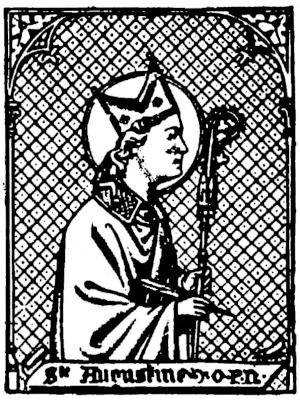
\includegraphics[width=45mm]{figures/titlepage-device.jpg}\par
    \vfill
    {\fontsize{18pt}{22pt}\selectfont BRUGIS\par}
    \vspace{2mm}
    {\fontsize{10pt}{13pt}\selectfont\textls[80]{MDCCCLXXVIII.}\par}
    \vspace*{8mm}
\end{titlepage}

% The two titlepage environments reset the page counter; realign it so
% the impressum (physical page 3) is folio iii and rectos carry odd
% roman folios throughout the front matter.
\setcounter{page}{3}
\thispagestyle{empty}
\vspace*{\fill}
\begin{flushleft}
\footnotesize
{\scshape Lexicon Latinum seu Corpus Phraseologiæ} \\
P.~Franc.~Wagner, S.J.; edidit Augustus Borgnet (in Belgio, anno MDCCCLXXVIII).\par\vspace{1em}
Hæc editio electronica ex transcriptione \textit{Project Gutenberg}
(libro electronico \#71280, die 26 mensis Julii anni 2023 emisso,
curantibus MWS, rmedinap atque sodalibus \textit{Online Distributed
Proofreading Team}) typis mandata est. Textus fontis in publico est;
licentia \textit{Project Gutenberg} ad ipsam transcriptionem
pertinet.\par\vspace{1em}
{\scshape Typographia:} litteris
\ifnum\dictuselexicon=1 \textit{Lexicon No1} (officinæ Enschedé)\else
\textit{XCharter} (ex \textit{Bitstream Charter} Matthæi Carter)\fi{}
composita, subsidiis \textit{Gentium} et \textit{DejaVu Serif},
litteris \textit{Charis SIL} ad phonetica; machina LuaLaTeX.\par\vspace{1em}
Insigne typographi in pagina tituli retinetur; cetera ornamenta
editionis impressæ non reproducuntur.\par\vspace{1em}
Typis mandatum anno MMXXVI.
\end{flushleft}

\thispagestyle{empty}
\vspace*{\fill}
\begin{center}
    \begin{minipage}{0.8\linewidth}
        \centering
        \itshape
        Textum huius voluminis transcriptoribus societatum
        \textup{Distributed Proofreaders} atque \textup{Project
        Gutenberg} debemus, litterarum autem formas
        \ifnum\dictuselexicon=1 Bram de Does\else Matthæo Carter\fi{}
        artifici. Utrisque gratias agimus.
    \end{minipage}
\end{center}
\vspace*{\fill}

\thispagestyle{plain}
\ctsection{Préface de la nouvelle édition}

\begin{otherlanguage}{french}
\begin{multicols}{2}
\textit{En réimprimant ce livre, fameux en Allemagne au siècle dernier, notre unique but a été de rendre aux vrais amis des études latines un ouvrage destiné à développer la connaissance du latin. Nous avons voulu offrir aux professeurs et aux élèves, surtout à ces derniers, un manuel vraiment pratique, pour approfondir les beautés intimes de la langue qui “ seule entre toutes les langues mortes, est véritablement ressuscitée, et qui UNE FOIS RESSUSCITÉE, NE MEURT PLUS!”}\footnote{de Maistre, \textit{Du Pape}.}

\textit{Avant d’indiquer le plan du livre et la manière de s’en servir utilement, qu’il nous soit permis de rappeler en quelques mots les principaux actes de la vie de l’auteur.}

\textit{ François Wagner naquit à Wangen, en Souabe, le 14 août 1675. Il fut admis dans la Compagnie de Jésus au noviciat de Krems à l’âge de 15 ans. Après avoir terminé ses deux années d’épreuve, il enseigna pendant plus de 25 ans la rhétorique, dans les colléges de Krems, de Presbourg et de Tyrnau. Étant recteur du Séminaire de Vienne, il dirigea une congrégation et s’occupa de la composition de plusieurs ouvrages estimés. Il mourut à Vienne, le 8 février 1738, à l’âge de 62 ans.}

\textit{Tels sont les détails que nous fournit sur cet homme illustre la Bibliothèque des écrivains de la Compagnie de Jésus. Le P. Jean Nép. Stœger, dans ses Scriptores Provinciæ Austriacæ Societatis Jesu, nous a transmis la liste complète des nombreux ouvrages écrits par le Père Wagner, qui tour à tour, s’occupant de rhétorique, de grammaire, de géographie, d’histoire, nous a laissé dans ces diverses branches des connaissances humaines, des traces remarquables de son esprit actif et pénétrant.}

\textit{Notre but, dans cet avertissement, est de parler seulement de son Dictionnaire de Phraséologie. Mais laissons l’auteur lui-même nous raconter comment naquit ce livre, nous indiquer ce qu’il a voulu en le composant, et de quelle manière il est parvenu à mener à terme l’ouvrage que nous possédons.}\footnote{Voici, d’après les Auteurs de la \textit{Bibliothèque des Écrivains de la Compagnie de Jésus}, Tome 3ᵉ, pages 1467, 1468 et 1469, (Louvain, MDCCCLXXVI) les principales éditions de l’ouvrage que nous offrons aujourd’hui au public:\par Universæ Phraseologiæ corpus congestum. Augustæ Vindelicorum, 1718.—Ratisbonæ, 1740, 8ᵒ.\par Universæ Phraseologiæ corpus congestum a P. Francisco Wagner, Societatis Jesu Sacerdote, secundis curis a quopiam ejusdem Societatis Sallustiana, Cæsareana, Liviana, Corneliana, etc., Phraseologiis locupletatum. Editio novissima, auctior et emendatior. Cum Privilegio Sacræ Cæsareæ Majestatis et Permissu Superiorum. Ratisbonæ, Sumptibus Emerici Felicis Baderi, A. P. C. N. MDCCXLV, 8ᵒ, \textit{pp.} 816 \textit{à 2 col.}, sll. \textit{L’épître dédicatoire, signée par l’auteur, est en date du 20 février 1718. La concession à l’imprimeur est du 4 janvier 1738. A la fin on a joint}: Latinitatis ars brevicula, seu syntaxis ornata, de tribus latinæ linguæ virtutibus, puritate, elegantia et copia, \textit{pp.} 82. Index diffusior vocum barbararum vel minus elegantium, \textit{p.} 1 \textit{à} 48. Index Germanico-Latinus \textit{p.} 49 \textit{à} 96.—\textit{Même titre.} Ratisbonæ, Sumptibus Emerici Felicis Baderi, A. P. C. N. MDCCLVIII, 8ᵒ, \textit{pp.} 808, 80 \textit{et} 85—\textit{Ibid.} id. 1751, 8ᵒ.\par Universæ Phraseologiæ Latinæ corpus congestum a P. Francisco Wagner, Societatis Jesu Sacerdote, secundis curis a quopiam ejusdem Societatis Sallustiana, Cæsareana, Liviana, Corneliana, etc., Phraseologiis ac denique Indice Verborum quæ in foro militari, civili sacroque obtinent, locupletatum. Editio Novissima, Auctior et Emendatior. Ratisbonæ et Viennæ, Sumptibus Emerici Felicis Baderi, 1760, 8ᵒ, \textit{pp.} 808 \textit{à} 2 \textit{col.} sll. \textit{A la fin on a joint}: Latinitatis ars brevicula, seu Syntaxis ornata, de tribus Latinæ linguæ virtutibus, puritate, elegantia et copia, \textit{pp.} 80. Index diffusior vocum barbararum, aut minus elegantium, \textit{p.} 1 \textit{à} 48. Index vocum quæ in foro militari, civili, sacroque obtinent. Ex Iano, Noltenio, d’Aquino, Seyboldo, Strada, Maffejo, Galutio, \textit{etc.}, collectus, \textit{p.} 49 \textit{à} 74. Index Germanico-Latinus, \textit{p.} 75 \textit{à} 111, \textit{fin du volume}.\par P. Francisci Wagner Universa Phraseologia Latina. Ab eodem secundis curis Sallustiana, Cæsareana, Liviana, Corneliana, etc. Phraseologiis ac denique Indice Verborum quæ in foro militari, civili sacroque obtinent, locupletata et ad usum juventutis litterarum studiosæ accommodata. Editio novissima, auctior et emendatior. Augustæ Vindelicorum, Sumptibus Matthæi Rieger p. m. filiorum. MDCCXCII, 8ᵒ, \textit{pp.} XVI \textit{à} 896. \textit{A la fin}: Latinitatis ars brevicula, \textit{etc.}, \textit{pp.} 204.\par Stœger dit: “Universæ.... Corpus auctum ab alio Sacerdote, S. J. Phraseologia Sallust. Cæsar. Liv. Cornel. etc., Augustæ Vindelicorum, 1801, 8ᵒ, et cum indice Viennæ, Geistinger, 1824, 8ᵒ.”\par Fr. Wagner Universa Phraseologia Latina, edit. novissima, Schmidt, Viennæ et Tergesti, 1824, 8ᵒ.\par Wagneri Universa Phraseologia Latina, aucta et emendata a Span. Viennæ, 1825.\par Adjecta Phraseologia Germanico-Latina a P. Goldhagen, S. J. cum Indice Verborum in foro sacro, civili et militari obtinentium. Moguntiæ, 1751, 1766, 8ᵒ.\par Wagner’s deutsch-lateinische Phraseologie, bearbeitet von Seibt, Prag. 1846.\par Universa Phraseologia Latina adjecta lingua hungarico slavonica. Tyrnaviæ, 1775, 8ᵒ.\par Franc. Wagneri Universæ Phraseologiæ corpus idiomate slavico locupletatum. Tyrnaviæ, 1750, 8ᵒ \textit{Par le P. B.} Zambal, S. J.\par Compendiaria methodus addiscendi tres præcipuas latinæ linguæ virtutes, Puritatem, Elegantiam et Copiam, in usum juventutis emendatæ latinitatis studiosæ proposita. Authore R. P. Francisco Wagner Societatis Jesu. Cum facultate superiorum. Dilingæ, Sumptibus Wilhelmi Hausen, anno 1735, 8ᵒ, \textit{pp.} 96.\par Supellex latinitatis ex Phraseologia Francisci Wagner, S. J. ad usum scholarum ejusdem Societatis collecta. Vilnæ, typ. Academ. S. J., 1751, 8ᵒ. (Editor est P. Fr. Bohomolec S. J., teste Ianocki.)—Idem, cum vocibus polonis. Calissii, typ. S. J., 1752, 12ᵒ.—Editio 2ᵃ Leopoli, typ. S. J., 1756, 8ᵒ, \textit{pp.} 42, 377 \textit{et} 54.—Vilnæ, typ. Academ. S. J., 1757, 12ᵒ.—Calissii, typ. S. J., 1772, 12ᵒ.\par Supellex latinitatis ex Phraseologia, P. Fr. Wagner S. J., ad usum scholarum ejusdem Societatis collecta. Editio 2ᵃ correctior. Leopoli, typ. S. J., 1756, 8ᵒ, \textit{pp.} 23 \textit{à} 77 \textit{et} 102.\par Outre ces 24 éditions, nous en possédons deux autres. La première appartient à la bibliothèque de St Acheul: Universæ, etc... Corpus, demum linguis Hungarica, Germanica et Slavica locupletatum. Budæ, typis typographiæ Regiæ Univers. Hungaricæ, 1822, 8ᵒ, 2 vol. \textit{pp.} 1524 à 83. L’autre, appartenant à la bibliothèque de l’École libre de la Providence, est un peu plus ancienne. C’est une réimpression de l’édition de 1792, faite chez Mathias Rieger, \textit{pp.} XVI \textit{à} 896; supp. 204. Augustæ Vindelicorum, MDCCC.}

\textit{“Étant professeur des jeunes religieux qui recommençaient leurs humanités, le but de tous mes soins était d’accomplir le sage précepte du P. Jouvency, sans contredit le premier parmi nous dans la connaissance parfaite de la langue latine,” Patris Juvencii, harum litterarum hodie inter nos facile Principis. “Le premier travail du maître, dit celui-ci, sera de montrer à ses élèves le style le plus pur et de les aider à l’acquérir. Je recherchais donc ce que je pouvais offrir de mieux à ces jeunes gens, pour les conduire aussi promptement que sûrement à l’acquisition des trois grandes qualités de la langue latine, la propriété, l’élégance, l’abondance. Pour la propriété, outre les Thesaurus, je faisais étudier tous les jours à mes élèves pendant un quart d’heure le Flos Latinitatis du P. Pomey, et au bout de deux mois, je remarquais des fruits merveilleux, jam intra bimestre Latinum quid velut in herba efflorescere, non sine jucundo animi sensu animadverti. Pour l’élégance, Tursellini, Schorus, Dolet, Hadrianus étaient les maîtres que je leur faisais étudier et copier. Enfin, pour l’abondance, Manusius, Bucher et Schönsleder. Mais, bientôt, je m’aperçus que cette foule de livres inondaient leurs pupitres, qu’ils perdaient un temps précieux à rechercher, ici les adverbes, là les épithètes ou les synonymes, ailleurs les développements, et c’est alors que je résolus de réunir avec ordre et méthode, dans un seul ouvrage, le fruit des veilles de tous ces hommes illustres.”}

\textit{C’est ainsi que naquit le Universæ Phraseologiæ corpus congestum. Il fut d’abord exclusivement composé de phrases et de tournures tirées de Cicéron, puis on y ajouta un petit nombre d’expressions appartenant aux grands auteurs du siècle d’or de la langue latine, Salluste, César, Tite-Live, Cornelius et quelques autres. Il faut remarquer que l’auteur ne cite pas toujours textuellement l’écrivain auquel il a emprunté sa citation, et c’est ce qui a empêché, dans cette édition, d’indiquer les sources, quoique nous puissions affirmer que nous avons vérifié presque toutes les citations au moyen de l’Apparatus de Nizzolius, de Forcellini et de Freund. Souvent il se contente de prendre la tournure et de l’appliquer au passage qu’il veut développer. Cependant, dans ce qui est rangé sous la rubrique Usus : les phrases qui servent à indiquer la Syntaxe particulière de chaque mot, sont empruntées textuellement à Cicéron et aux meilleurs auteurs du grand siècle. Souvent nous les avons rétablies et traduites, pour la plus grande utilité des élèves. “Leur lecture assidue, ajoute le P. Wagner, non-seulement donnera aux élèves les différentes significations d’un mot, mais encore leur prouvera que négliger d’en suivre la construction, c’est s’exposer à employer une tournure peu latine, “ si quampiam atque ab his alienam construendi formulam adhibuerint Discipuli, fere in Idiotismum se impactos admoneantur.”}

\textit{Mais il ne suffit pas d’avoir un bon livre, il faut savoir s’en servir; or, à première vue, il semble que l’usage de ce Dictionnaire ne soit pas accessible à tout le monde. Il est hors de doute, et l’expérience le prouve, que si l’on parvient à en saisir l’économie, si l’on en a, pour ainsi dire, la clef, on parviendra en peu de temps à faire de rapides progrès dans la connaissance de la langue latine. L’auteur en avait constaté l’efficacité, quand il nous dit: “ Noveram adolescentes qui orationem struerent tam elegantem, ut in volvendo Cicerone, multos annos posuisse videri potuissent hujus artificii ignari. Inest et illud commodi quod ea, quæ aliena fuerant, multiplici usu sua faciant; quodque dicitur, in succum et sanguinem suum vertant. ”}

\textit{Pour cela, il ne faut pas puiser indistinctement dans ce livre, coudre ensemble, sans suite et sans liens, des membres de phrase, qui, pris individuellement, sont très latins, mais qui doivent être rapprochés avec goût et discrétion. L’enfant intelligent doit faire sans dictionnaire son discours, sa narration ou son thème; il doit, après avoir médité profondément son sujet, après l’avoir ordonné dans toutes ses parties, l’écrire dans un latin plus ou moins pur, plus ou moins élégant, selon sa force et sa capacité. Ce travail, le plus important sans contredit, étant terminé, il devra, avec l’aide du dictionnaire de Phraséologie, débarrasser son devoir, que nous pouvons supposer correct, de toutes les tournures françaises, des gallicismes, des mots peu latins, et de cent autres imperfections, auxquelles il trouvera un remède assuré dans ce volume, s’il sait s’en servir avec intelligence et discernement.}

\textit{Montrons, par un exemple facile, la vraie manière d’user avec fruit de ce livre. C’est une lettre d’un fils à son père pour lui demander de l’argent, dans le but d’acheter des livres. Dans la première colonne, se trouve cette lettre dans le style d’un élève ordinaire de troisième; style simple et exempt de fautes contre les règles de la grammaire. Dans la seconde, la même lettre a été modifiée, rendue plus élégante au moyen du dictionnaire de Phraséologie. Du reste, les mots modifiés dans la première colonne sont soulignés, ce sont ceux-là qui doivent être l’objet du travail personnel de l’élève, quand il a jeté sur le papier les idées et qu’il veut donner à son style ce poli, cette perfection que demande la langue latine.}

\end{multicols}
\noindent\begin{minipage}[t]{0.48\textwidth}\small
\textit{Scio} equidem, te alioquin mei causa multos \textit{sumptus facere}; ausus tamen sum, novam insuper gratiam \textit{petere}. \textit{Suadet} nobis magister, ut libros quos in schola \textit{explicat, coemeremus, spondetque}, si eos domi \textit{legerimus}, multum profecturos. Uti hactenus semper \textit{conatus sum}, primo \textit{loco} aut primis proximus esse, ita nihil \textit{tristius} foret, quam si, ob hunc librorum defectum, priorem laudem \textit{amitterem} et a discipulis \textit{contemnerer}. \textit{Spero} autem in causa tam æqua, te, ut fuisti, erga me \textit{liberalem} fore.


\end{minipage}\hfill
\begin{minipage}[t]{0.48\textwidth}\small
Cognitum equidem habeo, multas alioquin impensas a te mei causa tolerari, id tamen mihi sumpsi, ut novam insuper gratiam etiam atque etiam a te contenderem. Auctor nobis fit magister, ut in coemendos eos libros, quos in schola nobis miro evolvit modo, pecuniæ aliquid collocaremus; fidemque suam obligat, fore ut, si eosdem domi etiam legendo contriverimus, magnos progressus faciamus. Uti hactenus nervis omnibus contendi, principem in schola locum vel primo proximum tenere, ita nihil tristitia majore me conficeret, atque si, ob hunc librorum defectum, priorum laudum jacturam facerem, et a condiscipulis despectui haberer. Spe autem ducor in causa tam æqua, fructus liberalitatis tuæ uberrimos, ut pervenere, ad me perventuros.


\end{minipage}

\begin{multicols}{2}
\textit{Après avoir souligné, dans mon devoir, les expressions qui me déplaisent, je cherche à les remplacer au moyen du dictionnaire de Phraséologie. Prenons, pour commencer, le verbe, scio ; à cet article nous trouverons: compertum habeo, cognitum habeo, etc. Donc compertum vel cognitum equidem habeo multas alioquin impensas a te mei causa tolerari, en substituant ce verbe passif, forme essentiellement latine, au verbe facere, gallicisme français, dans le sens de facere sumptus, faire des dépenses. Nous remplacerons, toujours au moyen de la Phraséologie, ausus tamen sum par id tamen mihi sumpsi, et à la place du gallicisme petere gratiam, nous mettrons contendere gratiam. Avec le verbe sumpsi suivi du subjonctif, nous terminerons ainsi la période: Id tamen mihi sumpsi ut novam insuper gratiam etiam atque etiam a te contenderem. C’est ainsi que nous trouverons dans le Dictionnaire tous les autres changements à faire. Tantôt ce sera le substantif, tantôt l’adjectif, le verbe ou même les dérivés, qui seront l’objet des remarques de l’élève studieux, et il est évident que l’habitude prise de corriger ainsi, pendant une heure, un discours de deux pages, ne pourra manquer de produire, en peu de temps, des fruits merveilleux. L’enfant sera heureux de reconnaître dans son latin quelques unes de ces tournures qu’on lui a appris à admirer, et il fera des progrès rapides, s’il parvient à se garder contre l’écueil opposé, de vouloir tout farcir d’élégances plus ou moins bien employées “ ne omnia Elegantiis farcire velit, sed ut condimentum parce inspergat et cum judicio, quo discernat quæ Phrasis, cui voci ejus sententiæ aptior sit.”}

\textit{Mais, me dira-t-on peut-être, à quoi bon cet amas et d’élégances, de tours propres à la langue latine, qui ne peut servir qu’à tromper professeurs et élèves, à égarer même ces derniers dans une forêt d’expressions dont ils ne sont pas capables de sentir la justesse et la portée? Ce double reproche serait sérieux, s’il était fondé. Pourquoi, dirai-je à mon tour, recommander aux élèves de choisir les expressions, les tournures les plus latines? Pourquoi ces cahiers où l’on recueille, jour par jour, les phrases les plus saillantes, les tournures les plus autorisées de la langue de Cicéron? Pourquoi ces leçons apprises chaque jour? Pourquoi ces imitations quotidiennes du prince des écrivains latins? Peut-être sera-t-il difficile, dans les commencements de saisir toute la portée du livre que nous offrons de nouveau au public lettré, mais un peu d’expérience en montrera certainement l’utilité. Ce livre a pour lui la sanction des années, et notre époque, quoique moins enthousiaste de la langue latine que les siècles précédents, conserve cependant assez de grands et nobles esprits, pour qu’il soit inutile de prouver l’utilité de l’étude des belles-lettres pour la véritable formation de l’homme et du chrétien.}

\textit{Nous ne pouvons terminer ce travail sans indiquer les améliorations apportées à cette première édition française.}

\textit{Les textes ont été revus soigneusement d’après trois éditions différentes. Quand ils étaient obscurs ou écourtés, ils ont été rétablis dans leur intégrité au moyen de Forcellini, de Freund ou des originaux, et traduits en français. Pour plus de clarté, on a établi des différences de caractères, qui permettent de trouver rapidement ce qu’on recherche. Ainsi que dans tous les lexiques modernes, la quantité a été indiquée sur les mots, pour permettre aux élèves d’observer la règle si importante de l’accent tonique.}

\textit{Trois Index complètent l’ouvrage: dans le premier, on a signalé les barbarismes les plus fréquents que peuvent commettre les élèves, et le mot latin qui les remplace. Le second est aussi curieux qu’instructif. Il rend une quantité de mots techniques et propres aux arts, aux sciences et à la jurisprudence.}

\textit{Le troisième et le plus important est l’Index Gallico-Latinus. Les mots ont été placés par ordre alphabétique, en prenant le nom comme base du classement. Sous le nom sont placés les verbes, les adjectifs, les adverbes, et ainsi d’un seul coup-d’œil on voit les relations entre la langue française et la langue latine, les changements qui peuvent se produire dans la traduction du substantif, de l’adjectif et du verbe. Ce travail n’est pas un Dictionnaire français-latin; nous n’avons voulu faire qu’un Index, qui renvoyât au Corpus Phraseologiæ.}

\textit{Puissent ces divers travaux, entrepris pour la plus grande gloire de DIEU, édités avec le plus grand soin, répondre au but que s’est proposé l’auteur en les composant! Puissent-ils être utiles aux maîtres et aux élèves, augmenter dans les cœurs des uns et des autres l’amour de la langue latine, et avec cet amour, le désir de défendre et de protéger toujours la gardienne et la protectrice du latin, Celle qui a tant fait pour le succès des bonnes études, l’Église de DIEU!}

\textit{ Amiens, École libre de la Providence, 23 mai 1878.}

\begin{center}\textit{En la fête du bienheureux martyr André Bobola, de la Compagnie de Jésus.}\end{center}

\begin{flushright}\textit{Aug. BORGNET, S. J.}\end{flushright}

\end{multicols}
\end{otherlanguage}
\clearpage
\thispagestyle{plain}
\ctsection{Præfatio}

\begin{multicols}{2}
Cum eorum, qui humaniores litteras repetebant, domesticæ scholæ præfectus fuissem, id propositum habebam maxime, et eo industriam omnem convertendam existimabam, ut P. Juvencii, harum litterarum hodie inter nos facile Principis, sapienti monito obtemperarem. Primus, ait ille, Magistri labor erit, Latinum stilum illis optimum demonstrare, et ut assequantur, adjuvare. Ergo putare mecum cœpi, quæ adjumenta offerrem præsentissima, queis viis Adolescentes non minus sciendi aviditate, quam ingenii præstantia, ad omnem hujus litteraturæ laudem paratissimos, ad Latinæ Linguæ Proprietatem, Elegantiam, Copiam quam celerrime commodissimeque perducerem.

\textit{Proprietatem} ut condiscerent, hoc est, e barbarie vulgaris sermonis sordibusque emergerent, præter expositos barbararum vocum Indices multiplices, si quam vocem suspectam haberent, \textit{Thesaurum Latinitatis}, seu \textit{Forum Romanum} consulerent, jussi. Ex eodem præcipuorum verborum syntaxin usumque Latinitatis proprium ipse exscripsi: quo labore perfunctus admoneor a Collega, dudum id a P. Pomæio in suis Flosculis præstitum. Etsi dolerem actum me egisse, deque libello tam pervulgato ignorasse puderet, in eamdem tamen cum viro egregio cogitationem, methodum ac prope verba incidisse mihi gratulabar. Hos ergo flores transcribendos dedi meis; seposui quot diebus quartam horulæ partem, qua suscitandos pertentarem singulos, constitutumque ejus diei pensum de memoria repeterem; si qua adhærerent, explicabam; difficiliora paradigmatis illustrabam; et fiebat, ut quotidianæ scriptionis argumento fere aliquid inserere possent. Atque hisce scriptionis, auditionis, exercitationis industriis jam intra bimestre Latinum quid velut in herba efflorescere, non sine jucundo animi sensu animadverti.

Ut vero ad \textit{Elegantiam} quoque perpolirentur, Tursellini particulas singulis, Schorum illis aut Doletum, Hadrianum aliis aut Goclenium, etc., ut copia erat, divisi, monuique, ne legerent duntaxat, sed lecta in chartam compendio referrent, quo memoriæ commendarent altius, quæ ab lectione sæpe, ut fit, minus intenta facile devolatura erant.

Ut \textit{Copiam} cum elegantia combiberent, Manutium a Buchlero auctum, et Schönslederum præbui, quos altera quavis periodo inspicerent, quorum opibus ad ornatum varietatemque nec timide et liberaliter tantisper uterentur, dum usu non admodum diutino in jus suum assererent quæ aliena fuerant, abjectisque centonibus, de suo liberum quid et nativum contexerent; cogitarent autem præterea: hæc incipientium subsidia ad proritandum duntaxat, Latinoque aliquo sapore imbuendum Tironum palatum excogitata; cæterum germanæ Latinitatis spem omnem in assidua Ciceronis, bonorumque ex aurea ætate Auctorum lectione collocandam; hos tanta cura pervolvendos velut si nihil peractum paratumque accepissent a majoribus, sed unis ipsis eruenda forent, quæ ex his venis tantis conatibus egessere, quidquid hactenus fuit Phraseologorum.

Hæc agenti cum illud incommodum videbatur, quod tot libellorum, queis Discipulorum pluteos onerarem, turba mihi undeunde corradenda esset, tum quod iisdem, dum hinc Adverbia, Epitheta inde, etc., fastidiose commendicant, plurimum utilissimi temporis volvendo revolvendoque inaniter elaberetur. Hoc tædio ut levaremur utrinque, optare cœpi, esset aliquis, qui sparsas has operas, eademque apud diversos repetita in unum quoddam corpus conflandi consilium caperet. Tot jam exstare Criticorum, Grammaticorum, Phraseologorum Indices, Enchiridia, Gazophylacia, Thesauros, Elegantias observavi, ut felicem se reputare posset is, quem tantam, tam paratam materiam in unum volumen certo ordine ac methodo ædificandi animus incesseret; feliciores vero fore Discipulos, qui in magno viæ compendio progressiones tamen celeriores facerent, nec jam per rivulos concursare deberent, quos in unum fontem Vir adeo beneficus corrivasset.

Externis vero nostris scholasticis quam ejusmodi opera non opportuna modo, sed necessaria foret omnino! Ciceronem, Ciceronem ex alto suggestus Juvenibus inclamamus magistri, in hunc velut regulam omnisque Latinitatis exemplum respicere, hunc legere, imitari et scribere jubemus, sed iis juvenibus, quorum parti maximæ, præter fragmenta quædam suæ classis scholastico libro (quamquam et hunc quam pauci emant) inserta nullus domi Cicero ; plurimis Terentii, Livii, Sallustii, etc. ipsa nomina peregrina, plerique, quid Nizzolius aut Forum Romanum hominis vel rei sint, perinde ut maragnonius quispiam ignorent. Et hos stimulis fodiemus? hos Latinos Ciceronianos effici volumus? qua autem ope, ad quem lydium lapidem suspectæ fidei voces explorent? barbaras secernant, melioribus commutent? unde colores, verasque pro adulterinis pigmentis elegantias petant? unde ad copiolam aliquam parandam vel Synonymiam exsugant? Huc certe flagitii vidi devenisse nonnullos, ut Epistolam, chriam, orationem scripturi \textit{in Synonymis}, \textit{Gradibus ad Parnassum}, etc. habitarent, qua re quid horribilius et ad corrumpendum stilum aptius excogitari possit? quod si opulentiores quidam filii familias circumfluant etiam natentque Ciceronibus, Terentiis, etc. quam pauci iis urantur igniculis, ut formulas inde, phrases, etc. in adversaria excerperent, justam animi contentionem ad exhaurienda principiorum ardua afferrent?

Eædem atque his majores difficultates, cum Poeticæ fores obsiderent, fuere qui \textit{Flavissas}, \textit{Synonyma}, \textit{Gradus ad Parnassum}, etc., præclara adeo adjumenta elaborarent, ut brevi tempore Poeticum aliquem colorem inde caloremque trahere multos experiamur. Quid est igitur, quod nemo dum ad Oratoriam gradientibus de tali adminiculo de gradibus ad rostra gratificatus est? quid? quod optarunt hoc multi, nemo optantibus morem gessit? quid autem (aiebam), quin tute hanc spartam occupas, et lexicon aliquod Phraseologicum, aut quodvis demum nomen habeat, vel ipse conficis, vel si per temporis angustias excludaris, typum denique et summas lineas designas, quas tali provocatione commoti alii depingant denique et absolvant.

Consilii dubium duæ res magnopere retrahebant, magnitudo laboris et ignobilitas. Infida utebar parumque firma valetudine. Operosæ scholæ quotidianæ vacui utilisque temporis relinquebant minimum; et informaveram nonnulla, quorum Auctor minimum dici possem, cum e præsenti opere præter diligentis scribæ nomen nihil ad me rediturum cernerem. Titubantem Collega meus, externorum Rhetorum Magister, Vir et morum et Latinitatis purissimæ candore longe suavissimus, P. Gabriel Wimmert, iteratis identidem hortatibus in proposito retinuit, tantoque promptiorem habuit, quod ejusmodi, ut ego sum, hominum genus, ab omni fumo alienissimum esse, idque pro honestissimo ducere debet, si, magno quidem suo impendio, quæstu minimo, plurimorum commodis servire possit.

Re deliberata Phraseologos, quos nancisci poteram, omnes tres in classes partior; horum alii \textit{Proprietatem} docerent, ut Niessii, Cellarii, Vossii, Vorstii, Borichii Commentarioli; alii \textit{Elegantiam} præstarent, ut Hadrianus, Valla, Doletus, Tursellinus, Schorus, Fabri, etc., \textit{Copiam} denique nonnulli suppeditarent, quorum chorum Manutius duceret et Schönslederus. Horum, inquam, operas omnes in unum Corpus cogendas, eximenda, quæ apud singulos præcipua essent, atque sub unum conspectum objicienda constitui, ea tamen adjecta conditione, ut ne voluminis moles ita excresceret, quin ab juvenibus in scholam ad statas scriptiones comportari posset. Hanc vero, quam vides, methodum mihi descripsi:

I. Nizzolium equidem pro solo operis stravi, ejusdemque ordinem alphabeticum sum secutus, quin tamen iisdem me carceribus includerem, iisdem religionibus obligarem; neque enim in ea sum hæresi, ut vel Ciceronem de omnibus argumentis disputasse, aut non iisdem cum Vitruvio, Varrone, Livio, Cæsare, etc., si de iisdem rebus loqui voluisset, vocabulis usurum fuisse, existimem. Quare aliorum quoque ex aurea ætate Auctorum voces adjeci, asterisco notatas, ut ab Ciceronianis secernantur, non quod fugiendæ essent. Totus enim in ea sum sententia, juvenes intra hujus ætatis limites constringendos, et a Plinianis, Senecianis, etc. omnino abstinendos. Intelligent autem, quam hic vocem non repererint, nullum habere idoneum Auctorem: atque adeo meliore commutandam.

II. Vocabula nihilominus \textit{sacra et religiosa} suis locis characterum forma diversa intexui, eademque e Pontano, quo nemo melius christiane simul et Latine loqui docet, Tympii opera collectis observationibus illustravi.

III. Per illud Cf. \textit{confer}, passim, qua eundum esset, præsignavi.

IV. Synonyma, ut in Nizzolio sunt, simpliciter adscripsi.

V. Contraria signo )( notata, ut quæ se ipsis offerrent, non erat, ut multa vestigatione conquirerem.

VI. Vocum, quas fere pro idem significantibus usurpat vulgus, elegantiores vero haud paulum notionibus inter se differre observant, \textit{Differentias}, e Laurentio Valla dedi aliquas, ac revera cœpi potius, et quid voluissem ostendi.

VII. Suam vocibus singulis syntaxim seu \textit{Usum} peculiarem, sententiis formulisque lectissimis e Nizzolio, Pomæio, aliisque multo discrimine decerptis attexui, quarum iterata lectio cum alias utilitates afferret, tum si quampiam atque ab his alienam construendi formulam adhibuerint Discipuli, fere in Idiotismum se impactos admoneantur.

VIII. Vulgatiores barbarismos seu Idiotismos Syntaxi Latinæ locis quibusdam e Schoro, etc. subjeci; ut venia sit ingenue confitenti, ubi minimum oportebat, præparcus fui; nec enim solum demonstranda erat via, qua incederent; sed infames quotidianis erroribus scopuli detegendi, ut suæ barbariei identidem admonerentur juvenes.

IX. Ad Copiam seu Phraseologiam quod attinet, nempe operis partem principem, ac discentibus desideratissimam, primæ Editiones nonnisi collectas Roterodami, Manutii, quique omnibus præstat, Schönslederi Phrases, paulum ad Juvenum captum deflexas habuere. In præsens opera cujusdam Collegæ mei, et tædii vere decumani labore, accessere Liviana, Cæsareana, Corneliana, Sallustiana, cum Indice diffusiore vocum barbararum, alioque Tironibus admodum desiderato Gallico-Latino; Opusque evasit ejusmodi, ut detrahi nihil, addi perparum possit. Ab viri modestia obtinere non potui, ut suum de studiosa Juventute tam præclare meriti nomen adscribi pateretur.

Habetis hic humaniorum litterarum Professores, quo consilio primum cœptum sit Opus, et quantum ad ejus absolutionem recens accesserit. Si præterquam quid præstiterimus, quid insuper voluerimus, apud vos existimabitis, laboribus nostris, vestro vestrorumque commodo benevoli utemini, fruemini.

\end{multicols}

% print our abbreviations page
% The table is a longtable and may span several pages, so \thispagestyle
% would only affect the first: switch to plain (footer only, like the
% foreword) and restore fancy once the last table page has shipped out.
\pagestyle{plain}
\ctsection{Explications des signes et abréviations}
\printabbreviations{abbreviations.csv}
\clearpage
\pagestyle{fancy}
\thispagestyle{plain}
\ctsection{De hac editione}

Hæc editio totum Phraseologiæ Wagnerianæ corpus --- articulos 11\,239
--- ex editione Belgica anni MDCCCLXXVIII repetit. Suus cuique articulo
servatur apparatus: interpretationes Gallicæ litteris
inclinatis, synonyma (\dictlabel{syn.}), contraria (signo \mbox{)(}\,
notata), adverbia (\dictlabel{adv.}), epitheta (\dictlabel{epith.}),
phrases evolvendæ (\dictlabel{phras.}), usus auctorum
(\dictlabel{usus}) cum acceptionibus numeratis, notæque interdum
adiectæ (\dictlabel{vulg.}, \dictlabel{prov.}, \dictlabel{rad.},
\dictlabel{differ.}). Asteriscus voces ab auctore pro non Ciceronianis
habitas distinguit; parentheses locutiones vulgares includunt.

Lectiones mendosæ, etiam in præfatione Latina atque indicibus,
emendatæ sunt. Lectiones priores una cum emendationum rationibus et
testimoniis in commentario separato referuntur; emendationes ex
conjectura factæ a lectionibus testimoniis confirmatis distinguuntur.
In præfatione \textit{tum quod} et \textit{suppeditarent} ex conjectura
recepta sunt. In articulo \textit{accio}, pro \textit{exultro} legitur
\textit{ultro}; in indice Gallico-Latino, omisso \textit{Affermo},
\textit{loco} servatur.

Quantitates vocalium, ubi satis certa testimonia suppetunt, correctæ
sunt. Ubi de quantitate vocalis auctoritates dissentiunt vel
testimonia non sufficiunt, signum dubium omittitur: vocalis sine
signo neque longa neque brevis eo ipso declaratur. In lemmatibus
\textit{gratuitus} et \textit{istiusmodi} quantitas usitatior exhibetur;
brevior tamen vocalis apud poetas admittitur (\textit{gratuitum},
Statius, \textit{Silvæ} 1.6.16; genitivus in \textit{-ius}, Allen et
Greenough, \S~603). Scriptura \textit{quatuor}, quam Gaffiot quoque
admittit, servatur.

Tres indices historici editionis anni MDCCCLXXVIII volumen claudunt,
ut in originali: index vocum barbararum cum Latinis earum
æquivalentibus, index vocum quæ in foro militari, civili sacroque
obtinent, et index Gallico-Latinus.

\medskip
\noindent\textit{De usu vocabulorum.}
\textit{Etesiæ} plerumque masculino genere dicuntur; femininum tamen
apud Hyginum et Isidorum invenitur (Gaffiot; Georges).
\textit{Planeta} apud auctores classicos masculinum est; apud scriptores
medii ævi etiam femininum reperitur (\textit{Dictionary of Medieval
Latin from British Sources}). Utriusque vocabuli genus femininum,
quod hæc editio tradit, servatum est.
\textit{Obsurdeo}, in indice Gallico-Latino positum, etiam in
vocabulario quod Joris van Gheel anno MDCLII conscripsit legitur;
pro \textit{obsurdesco} usurpatum retinetur.
Genitivus pluralis \textit{sudium}, in indice rerum militarium
servatus, apud Sidonium quoque legitur (\textit{Epistulæ} 7.1.2).

\medskip
\noindent\textit{De præfatione Gallica.}
Locutio \textit{facere sumptus}, quam præfatio Gallica reprehendit,
non est per se a Latinitate aliena: Cicero ipse \textit{sumptum faciat}
(\textit{De imperio Cn. Pompei} 39) et \textit{sumptum in rem militarem
facere} (\textit{Ad familiares} 12.30.4) scripsit. Auctoris judicium
historicum servatur, sed hac nota definitur.
\vspace{1.5pc}

% build the lexicon from our csv
% NOTE: \twocolumn performs its own \clearpage; do not add
% \cleardoublepage before it (the pair would push the corpus one page
% further, onto a verso). With the current front matter, folio 1 lands
% on a recto and mirrored-margin parity matches physical parity --
% re-check if front-matter pages are ever added or removed.
\twocolumn
\pagenumbering{arabic}
\builddictionary{wagner-lat-fra.csv}
\clearpage
\raggedbottom % allow underfull vbox in the back matter
% The three historic indexes of the 1878 edition replace the generated
% makeindex section. Static running heads per index: clear BOTH
% guide-word fields (the dictword marks stop updating here and would
% otherwise show the last dictionary page's words).
\fancyhead[R]{}
\fancyhead[L]{\small\scshape index vocum barbararum}
\thispagestyle{plain}
\ctsection{index vocum barbararum}

\par{\dictfontsize\hangindent=1.5em\hangafter=1\noindent \textit{Ab antiquo.} Antiquitus.\par}
\par{\dictfontsize\hangindent=1.5em\hangafter=1\noindent \textit{Ab initio mundi.} Post homines natos, post hominum memoriam.\par}
\par{\dictfontsize\hangindent=1.5em\hangafter=1\noindent \textit{Ab initio rem repetere.} A capite, ab ultima ætate, memoria; altius rem arcessere; ab origine primisque causis rem repetere.\par}
\par{\dictfontsize\hangindent=1.5em\hangafter=1\noindent \textit{Ab invicem.} Inter se timere, distare.\par}
\par{\dictfontsize\hangindent=1.5em\hangafter=1\noindent \textit{Abominabilis.} Abominandus, detestabilis, exsecrabilis.\par}
\par{\dictfontsize\hangindent=1.5em\hangafter=1\noindent \textit{Abortire.} Partum abigere, abortum facere.\par}
\par{\dictfontsize\hangindent=1.5em\hangafter=1\noindent \textit{Abscindere reditum, annonam.} Receptu commeatuque aliquem intercludere.\par}
\par{\dictfontsize\hangindent=1.5em\hangafter=1\noindent \textit{Absentare se.} Subducere sese.\par}
\par{\dictfontsize\hangindent=1.5em\hangafter=1\noindent \textit{Absolvere ab hæresi.} Expiare ab hæresi, Ecclesiæ reconciliare.\par}
\par{\dictfontsize\hangindent=1.5em\hangafter=1\noindent \textit{Absolute.} Præcise, simpliciter negare.\par}
\par{\dictfontsize\hangindent=1.5em\hangafter=1\noindent \textit{Absone.} Absurde.\par}
\par{\dictfontsize\hangindent=1.5em\hangafter=1\noindent \textit{Absurditas.} Res absurda.\par}
\par{\dictfontsize\hangindent=1.5em\hangafter=1\noindent \textit{Acceptare officium.} Suscipere munus.\par}
\par{\dictfontsize\hangindent=1.5em\hangafter=1\noindent \textit{Acclinis} (poet.) Inclinatus, reclinatus.\par}
\par{\dictfontsize\hangindent=1.5em\hangafter=1\noindent \textit{Acedia.} Pigritia, negligentia.\par}
\par{\dictfontsize\hangindent=1.5em\hangafter=1\noindent \textit{Acervare.} Cumulare.\par}
\par{\dictfontsize\hangindent=1.5em\hangafter=1\noindent \textit{Acquisitio.} Comparatio.\par}
\par{\dictfontsize\hangindent=1.5em\hangafter=1\noindent \textit{Activitas.} Solertia, industria, velocitas.\par}
\par{\dictfontsize\hangindent=1.5em\hangafter=1\noindent \textit{Ad diem præfixam.} Ad diem, ad diem dictum, ad statum diem.\par}
\par{\dictfontsize\hangindent=1.5em\hangafter=1\noindent \textit{Adhuc semel.} Iterum.\par}
\par{\dictfontsize\hangindent=1.5em\hangafter=1\noindent \textit{Ad instar.} Instar.\par}
\par{\dictfontsize\hangindent=1.5em\hangafter=1\noindent \textit{Adinventio.} Inventio.\par}
\par{\dictfontsize\hangindent=1.5em\hangafter=1\noindent \textit{Adversitas.} Res afflictæ, res adversæ, casus adversi, res turbidæ, asperæ.\par}
\par{\dictfontsize\hangindent=1.5em\hangafter=1\noindent \textit{Ad vivum exprimere.} Scite, miro artificio exprimere.\par}
\par{\dictfontsize\hangindent=1.5em\hangafter=1\noindent \textit{Adunare.} Conjungere, congregare.\par}
\par{\dictfontsize\hangindent=1.5em\hangafter=1\noindent \textit{Ædificare alios.} Bono esse exemplo.\par}
\par{\dictfontsize\hangindent=1.5em\hangafter=1\noindent \textit{Affabiliter.} Blande, comiter.\par}
\par{\dictfontsize\hangindent=1.5em\hangafter=1\noindent \textit{Affirmative.} Affirmate.\par}
\par{\dictfontsize\hangindent=1.5em\hangafter=1\noindent \textit{Albedo.} Candor, albus color.\par}
\par{\dictfontsize\hangindent=1.5em\hangafter=1\noindent \textit{Aliqualiter.} Aliquomodo, quodammodo.\par}
\par{\dictfontsize\hangindent=1.5em\hangafter=1\noindent \textit{A longe.} Procul, eminus.\par}
\par{\dictfontsize\hangindent=1.5em\hangafter=1\noindent \textit{A longo tempore.} Jam dudum, pridem.\par}
\par{\dictfontsize\hangindent=1.5em\hangafter=1\noindent \textit{Alta voce.} Clara voce.\par}
\par{\dictfontsize\hangindent=1.5em\hangafter=1\noindent \textit{Alternatim.} Alternis vicibus.\par}
\par{\dictfontsize\hangindent=1.5em\hangafter=1\noindent \textit{Amantissimus frater meus.} Carissimus; dicitur tamen active: mei amantissimus.\par}
\par{\dictfontsize\hangindent=1.5em\hangafter=1\noindent \textit{Amittere prœlium.} Prœlio inferiorem discedere, adversum prœlium facere; vinci.\par}
\par{\dictfontsize\hangindent=1.5em\hangafter=1\noindent \textit{Amodo.} Deinceps, posthac.\par}
\par{\dictfontsize\hangindent=1.5em\hangafter=1\noindent \textit{Amphibologia.} Amphibolia.\par}
\par{\dictfontsize\hangindent=1.5em\hangafter=1\noindent \textit{Angariare.} Cogere, adigere, compellere.\par}
\par{\dictfontsize\hangindent=1.5em\hangafter=1\noindent \textit{Animalculum.} Bestiola.\par}
\par{\dictfontsize\hangindent=1.5em\hangafter=1\noindent \textit{Antecessores.} Majores.\par}
\par{\dictfontsize\hangindent=1.5em\hangafter=1\noindent \textit{Ante judicem vocare aliquem.} In judicium vocare aliquem.\par}
\par{\dictfontsize\hangindent=1.5em\hangafter=1\noindent \textit{Ante omnia.} Imprimis, præ cæteris.\par}
\par{\dictfontsize\hangindent=1.5em\hangafter=1\noindent \textit{Apostatare.} Nuntium remittere Religioni, ejurare Sacra, deficere a fide Christo data.\par}
\par{\dictfontsize\hangindent=1.5em\hangafter=1\noindent \textit{Apparuit in somno.} Vidi secundum quietem, spectaculum habui in somno, per quietem spectandum se mihi obtulit.\par}
\par{\dictfontsize\hangindent=1.5em\hangafter=1\noindent \textit{Appellit navis.} Appellitur navis, nauta appellit.\par}
\par{\dictfontsize\hangindent=1.5em\hangafter=1\noindent \textit{Approximatio.} Appropinquatio, accessus.\par}
\par{\dictfontsize\hangindent=1.5em\hangafter=1\noindent \textit{Aptitudo.} Habilitas.\par}
\par{\dictfontsize\hangindent=1.5em\hangafter=1\noindent \textit{Aquaticus} (poet.). Aquatilis, aquarum incola.\par}
\par{\dictfontsize\hangindent=1.5em\hangafter=1\noindent \textit{Armistitium.} Induciæ.\par}
\par{\dictfontsize\hangindent=1.5em\hangafter=1\noindent \textit{Attemperare.} Moderari, adaptare.\par}
\par{\dictfontsize\hangindent=1.5em\hangafter=1\noindent \textit{Austeritas vitæ.} Victus cultusque asperior.\par}
\par{\dictfontsize\hangindent=1.5em\hangafter=1\noindent \textit{Auxiliator.} Adjutor.\par}
\par{\dictfontsize\hangindent=1.5em\hangafter=1\noindent \textit{Axioma.} Pronuntiatum, effatum.\par}
\par{\dictfontsize\hangindent=1.5em\hangafter=1\noindent \textit{Baccalaureus.} Prima laurea donatus.\par}
\par{\dictfontsize\hangindent=1.5em\hangafter=1\noindent \textit{Benedicere populo.} Bene precari populo, fausta cum prece dimittere, pacem et veniam a Superis precari.\par}
\par{\dictfontsize\hangindent=1.5em\hangafter=1\noindent \textit{Benefactor.} Beneficus, munificus, patronus.\par}
\par{\dictfontsize\hangindent=1.5em\hangafter=1\noindent \textit{Beneplacitum.} Arbitratus, voluntas, nutus, libido.\par}
\par{\dictfontsize\hangindent=1.5em\hangafter=1\noindent \textit{Bene sit.} Benigne sit.\par}
\par{\dictfontsize\hangindent=1.5em\hangafter=1\noindent \textit{Bene vivere.} Pure casteque vitam colere; \textit{vel} laute indulgenterque vivere.\par}
\par{\dictfontsize\hangindent=1.5em\hangafter=1\noindent \textit{Bestialis.} Brutus, inhumanus, bruto conveniens.\par}
\par{\dictfontsize\hangindent=1.5em\hangafter=1\noindent \textit{Biformis} (poet.). Biformatus.\par}
\par{\dictfontsize\hangindent=1.5em\hangafter=1\noindent \textit{Blanditor.} Adulator, assentator.\par}
\par{\dictfontsize\hangindent=1.5em\hangafter=1\noindent \textit{Blasphemare.} Impias in DEUM voces mittere, scelesta lingua DEUM lacessere.\par}
\par{\dictfontsize\hangindent=1.5em\hangafter=1\noindent \textit{Bona opera facere.} Virtutum officiis fungi.\par}
\par{\dictfontsize\hangindent=1.5em\hangafter=1\noindent \textit{Bonæ conscientiæ est.} Animi integerrimi; mente nullius culpæ sibi conscia.\par}
\par{\dictfontsize\hangindent=1.5em\hangafter=1\noindent \textit{Brutum.} Bestia, animal, pecus.\par}
\par{\dictfontsize\hangindent=1.5em\hangafter=1\noindent \textit{Calendarium.} Fasti.\par}
\par{\dictfontsize\hangindent=1.5em\hangafter=1\noindent \textit{Calumniose.} Per calumniam, injuriam.\par}
\par{\dictfontsize\hangindent=1.5em\hangafter=1\noindent \textit{Campana.} Æs campanum.\par}
\par{\dictfontsize\hangindent=1.5em\hangafter=1\noindent \textit{Carnalis homo.} Libidini, voluptatibus deditus.\par}
\par{\dictfontsize\hangindent=1.5em\hangafter=1\noindent \textit{Cautela.} Cautio.\par}
\par{\dictfontsize\hangindent=1.5em\hangafter=1\noindent \textit{Christianitas.} Res christiana, Respublica christiana, Orbis christianus.\par}
\par{\dictfontsize\hangindent=1.5em\hangafter=1\noindent \textit{Christianus.} Christi Sectator, Christi disciplinam professus \textit{vel} nomen christianum.\par}
\par{\dictfontsize\hangindent=1.5em\hangafter=1\noindent \textit{Circumlocutio.} Circuitio verborum, circumscriptio.\par}
\par{\dictfontsize\hangindent=1.5em\hangafter=1\noindent \textit{Circumstantia.} Res attributæ, adjuncta loci temporisque ratio.\par}
\par{\dictfontsize\hangindent=1.5em\hangafter=1\noindent \textit{Circumvallatio.} Locus aggere ambitus, limes extimus, circuitus, munimenta castrorum.\par}
\par{\dictfontsize\hangindent=1.5em\hangafter=1\noindent \textit{Claudere epistolam.} Obsignare.\par}
\par{\dictfontsize\hangindent=1.5em\hangafter=1\noindent \textit{Coacte.} Per vim, vi adactus, adductus.\par}
\par{\dictfontsize\hangindent=1.5em\hangafter=1\noindent \textit{Coœtaneus.} Æqualis ejusdem temporis.\par}
\par{\dictfontsize\hangindent=1.5em\hangafter=1\noindent \textit{Cœlicus.} Cœlestis.\par}
\par{\dictfontsize\hangindent=1.5em\hangafter=1\noindent \textit{Cœlitus.} De cœlo, divinitus.\par}
\par{\dictfontsize\hangindent=1.5em\hangafter=1\noindent \textit{Commendare DEO negotium in oratione.} Consulere per preces DEUM.\par}
\par{\dictfontsize\hangindent=1.5em\hangafter=1\noindent \textit{Communicare.} Ad Sacram Synaxim, mensam, panem cœlestem accedere, divino Epulo pasci.\par}
\par{\dictfontsize\hangindent=1.5em\hangafter=1\noindent \textit{Communiter} pro. Plerumque, vulgo.\par}
\par{\dictfontsize\hangindent=1.5em\hangafter=1\noindent \textit{Comparative.} Comparate.\par}
\par{\dictfontsize\hangindent=1.5em\hangafter=1\noindent \textit{Comparere ante aliquem.} Sistere se alicui.\par}
\par{\dictfontsize\hangindent=1.5em\hangafter=1\noindent \textit{Compassio.} Commiseratio, misericordia.\par}
\par{\dictfontsize\hangindent=1.5em\hangafter=1\noindent \textit{Compati.} Commoveri, capi, affici misericordia; dolere casum, vices alterius.\par}
\par{\dictfontsize\hangindent=1.5em\hangafter=1\noindent \textit{Complexio} † pro. Corporis constitutio, humorum temperamentum, corporis habitudo.\par}
\par{\dictfontsize\hangindent=1.5em\hangafter=1\noindent \textit{Conceptus mentis.} Sensa mentis, cogitata mentis.\par}
\par{\dictfontsize\hangindent=1.5em\hangafter=1\noindent \textit{Concivis.} Civis, municeps.\par}
\par{\dictfontsize\hangindent=1.5em\hangafter=1\noindent \textit{Concupiscentia.} Cupiditas, libido.\par}
\par{\dictfontsize\hangindent=1.5em\hangafter=1\noindent \textit{Confabulatio.} Collocutio, sermones.\par}
\par{\dictfontsize\hangindent=1.5em\hangafter=1\noindent \textit{Confidentia} † pro. Fiducia.\par}
\par{\dictfontsize\hangindent=1.5em\hangafter=1\noindent \textit{Confortare.} Corroborare, confirmare.\par}
\par{\dictfontsize\hangindent=1.5em\hangafter=1\noindent \textit{Confusus.} Pudefactus.\par}
\par{\dictfontsize\hangindent=1.5em\hangafter=1\noindent \textit{Congrue.} Congruenter.\par}
\par{\dictfontsize\hangindent=1.5em\hangafter=1\noindent \textit{Congruus.} Congruens.\par}
\par{\dictfontsize\hangindent=1.5em\hangafter=1\noindent \textit{Conregnare.} Simul regnare.\par}
\par{\dictfontsize\hangindent=1.5em\hangafter=1\noindent \textit{Consequenter.} Porro, quod ex eo consequitur.\par}
\par{\dictfontsize\hangindent=1.5em\hangafter=1\noindent \textit{Contemporaneus.} Ejusdem temporis, ætatis.\par}
\par{\dictfontsize\hangindent=1.5em\hangafter=1\noindent \textit{Contentus est.} Sorte, rebus suis contentus est.\par}
\par{\dictfontsize\hangindent=1.5em\hangafter=1\noindent \textit{Contiguus} (poet.). Continens, contingens, \textit{vel} proximus, vicinus.\par}
\par{\dictfontsize\hangindent=1.5em\hangafter=1\noindent \textit{Continue.} Continenter.\par}
\par{\dictfontsize\hangindent=1.5em\hangafter=1\noindent \textit{Contradicere sibi.} Pugnantia loqui, secum ipso pugnare.\par}
\par{\dictfontsize\hangindent=1.5em\hangafter=1\noindent \textit{Controverti.} In controversia esse; in controversiam venire, deduci, vocari.\par}
\par{\dictfontsize\hangindent=1.5em\hangafter=1\noindent \textit{Conventio.} Conventus, \textit{vel} conventum.\par}
\par{\dictfontsize\hangindent=1.5em\hangafter=1\noindent \textit{Convitiari.} Proscindere convitio.\par}
\par{\dictfontsize\hangindent=1.5em\hangafter=1\noindent \textit{Coopertorium.} Tegumentum, operculum.\par}
\par{\dictfontsize\hangindent=1.5em\hangafter=1\noindent \textit{Coordinare.} Suo quodvis ordine collocare.\par}
\par{\dictfontsize\hangindent=1.5em\hangafter=1\noindent \textit{Cor} †. Animus, ratio, mens.\par}
\par{\dictfontsize\hangindent=1.5em\hangafter=1\noindent \textit{Corporis necessitates.} Necessaria vitæ præsidia; res ad vitam \textit{vel} usus necessarios requisitæ.\par}
\par{\dictfontsize\hangindent=1.5em\hangafter=1\noindent \textit{Correcte.} Emendate.\par}
\par{\dictfontsize\hangindent=1.5em\hangafter=1\noindent \textit{Creatura.} Res creata, res condita ab opifice et ædificatore mundi DEO.\par}
\par{\dictfontsize\hangindent=1.5em\hangafter=1\noindent \textit{Crescit malum.} Malum in dies ingravescit.\par}
\par{\dictfontsize\hangindent=1.5em\hangafter=1\noindent \textit{Crucem facere.} Signum crucis digito in fronte effingere, salutari se signo munire.\par}
\par{\dictfontsize\hangindent=1.5em\hangafter=1\noindent \textit{Cum tempore.} Progressu temporis, procedente tempore, tempore.\par}
\par{\dictfontsize\hangindent=1.5em\hangafter=1\noindent \textit{Cumulatim.} Cumulate.\par}
\par{\dictfontsize\hangindent=1.5em\hangafter=1\noindent \textit{Damnare ad mortem.} Damnare capitis \textit{vel} capite.\par}
\par{\dictfontsize\hangindent=1.5em\hangafter=1\noindent \textit{Dare licentiam.} Potestatem facere.\par}
\par{\dictfontsize\hangindent=1.5em\hangafter=1\noindent \textit{Debiti solutionem petere.} Admonere debitores, appellare de pecunia, nomina exigere.\par}
\par{\dictfontsize\hangindent=1.5em\hangafter=1\noindent \textit{Deceptor.} Veterator, circumscriptor.\par}
\par{\dictfontsize\hangindent=1.5em\hangafter=1\noindent \textit{Decimus nonus.} Undevicesimus.\par}
\par{\dictfontsize\hangindent=1.5em\hangafter=1\noindent \textit{Dedecens.} Turpis, indecorus.\par}
\par{\dictfontsize\hangindent=1.5em\hangafter=1\noindent \textit{De die in diem.} Indies; dicitur tamen diem ex die ducere, proferre, procrastinare.\par}
\par{\dictfontsize\hangindent=1.5em\hangafter=1\noindent \textit{Defectus.} Vitium ædium, etc.\par}
\par{\dictfontsize\hangindent=1.5em\hangafter=1\noindent \textit{Deitas.} Divinitas.\par}
\par{\dictfontsize\hangindent=1.5em\hangafter=1\noindent \textit{Delator.} Index, accusator.\par}
\par{\dictfontsize\hangindent=1.5em\hangafter=1\noindent \textit{Delectabilis.} Quod habet delectationem.\par}
\par{\dictfontsize\hangindent=1.5em\hangafter=1\noindent \textit{Dependere ab aliquo.} Pendere ex aliquo.\par}
\par{\dictfontsize\hangindent=1.5em\hangafter=1\noindent \textit{Deponere officium.} Deponere munus; abire, decedere magistratu.\par}
\par{\dictfontsize\hangindent=1.5em\hangafter=1\noindent \textit{Deprædari.} Prædari, spoliare, diripere.\par}
\par{\dictfontsize\hangindent=1.5em\hangafter=1\noindent \textit{Desertum.} Locus desertus, solitudo; locus humano cultu vacuus, solitudine et inopia vastus.\par}
\par{\dictfontsize\hangindent=1.5em\hangafter=1\noindent \textit{Desuescere.} Consuetudinem deponere, desuefacere.\par}
\par{\dictfontsize\hangindent=1.5em\hangafter=1\noindent \textit{Detractor.} Obtrectator.\par}
\par{\dictfontsize\hangindent=1.5em\hangafter=1\noindent \textit{Detractoria verba.} Famæ adversantia, inimica nomini, honorem lædentia, violantia.\par}
\par{\dictfontsize\hangindent=1.5em\hangafter=1\noindent \textit{Detrahere aliquid de pretio.} Deducere de summa.\par}
\par{\dictfontsize\hangindent=1.5em\hangafter=1\noindent \textit{De verbo ad verbum.} Ad verbum, verbum de verbo, totidem verbis.\par}
\par{\dictfontsize\hangindent=1.5em\hangafter=1\noindent \textit{Dictio} † pro. Vocabulum.\par}
\par{\dictfontsize\hangindent=1.5em\hangafter=1\noindent \textit{Discooperire.} Non tegere, retegere.\par}
\par{\dictfontsize\hangindent=1.5em\hangafter=1\noindent \textit{Discretio.} Prudentia in discrimine faciendo, delectus ac judicium.\par}
\par{\dictfontsize\hangindent=1.5em\hangafter=1\noindent \textit{Disparere.} Evanescere, sublimem abire, oculis subito subduci.\par}
\par{\dictfontsize\hangindent=1.5em\hangafter=1\noindent \textit{Disparitas.} Ratio dispar, diversa.\par}
\par{\dictfontsize\hangindent=1.5em\hangafter=1\noindent \textit{Dispositio animi.} Animi comparatio, affectio.\par}
\par{\dictfontsize\hangindent=1.5em\hangafter=1\noindent \textit{Disquirere.} Exquirere.\par}
\par{\dictfontsize\hangindent=1.5em\hangafter=1\noindent \textit{Dissitus} † pro. Disjunctus, longinquus, remotus; dicitur recte pro dispersus.\par}
\par{\dictfontsize\hangindent=1.5em\hangafter=1\noindent \textit{Ditescere.} Divitem fieri.\par}
\par{\dictfontsize\hangindent=1.5em\hangafter=1\noindent \textit{Diversimode.} Varie, alio atque alio modo, non uno modo.\par}
\par{\dictfontsize\hangindent=1.5em\hangafter=1\noindent \textit{Diversitas.} Varietas, dissimilitudo.\par}
\par{\dictfontsize\hangindent=1.5em\hangafter=1\noindent \textit{Divisim.} Seorsim, separatim.\par}
\par{\dictfontsize\hangindent=1.5em\hangafter=1\noindent \textit{Diutius sex mensibus.} Amplius sex menses.\par}
\par{\dictfontsize\hangindent=1.5em\hangafter=1\noindent \textit{Dono mittere rem.} Donare, munera mittere.\par}
\par{\dictfontsize\hangindent=1.5em\hangafter=1\noindent \textit{Dubietas.} Dubium.\par}
\par{\dictfontsize\hangindent=1.5em\hangafter=1\noindent \textit{Dubito, an non.} Dubito an facturus sim, haud scio an dicturus.\par}
\par{\dictfontsize\hangindent=1.5em\hangafter=1\noindent \textit{Echo} (poet.). Saxa et solitudines voci respondentia, vox aut sonus repercussus, valles clamoribus repercussæ.\par}
\par{\dictfontsize\hangindent=1.5em\hangafter=1\noindent \textit{E contra.} Contra, e contrario, contra ea, ex contraria parte.\par}
\par{\dictfontsize\hangindent=1.5em\hangafter=1\noindent \textit{Efformare.} Effingere, exprimere, formare.\par}
\par{\dictfontsize\hangindent=1.5em\hangafter=1\noindent \textit{Elapso anno.} Anno superiore.\par}
\par{\dictfontsize\hangindent=1.5em\hangafter=1\noindent \textit{Elucescit.} Lucet, lucescit.\par}
\par{\dictfontsize\hangindent=1.5em\hangafter=1\noindent \textit{Enervis.} Enervatus.\par}
\par{\dictfontsize\hangindent=1.5em\hangafter=1\noindent \textit{Eremus} †. Inculta solitudo, locus desertus.\par}
\par{\dictfontsize\hangindent=1.5em\hangafter=1\noindent \textit{Essentia rei.} Natura, vis, potestas rei.\par}
\par{\dictfontsize\hangindent=1.5em\hangafter=1\noindent \textit{Evaginare gladium.} Gladium stringere, e vagina educere.\par}
\par{\dictfontsize\hangindent=1.5em\hangafter=1\noindent \textit{Exaltare aliquem.} Efferre, provehere ad honores.\par}
\par{\dictfontsize\hangindent=1.5em\hangafter=1\noindent \textit{Examen conscientiæ facere.} Sua dicta factaque recognoscere, excutere conscientiam, in se inquirere, explorare animi latebras.\par}
\par{\dictfontsize\hangindent=1.5em\hangafter=1\noindent \textit{Exaudire} pro. Votis precibusque annuere, preces ratas habere.\par}
\par{\dictfontsize\hangindent=1.5em\hangafter=1\noindent \textit{Exercere virtutem.} Declarare, ostendere.\par}
\par{\dictfontsize\hangindent=1.5em\hangafter=1\noindent \textit{Ex nunc.} Ex hoc.\par}
\par{\dictfontsize\hangindent=1.5em\hangafter=1\noindent \textit{Exoptabilis.} Optabilis.\par}
\par{\dictfontsize\hangindent=1.5em\hangafter=1\noindent \textit{Exponere se periculo.} Offerre se periculis, committere.\par}
\par{\dictfontsize\hangindent=1.5em\hangafter=1\noindent \textit{Ex professo.} Consulto, de \textit{vel} ex industria, dedita opera.\par}
\par{\dictfontsize\hangindent=1.5em\hangafter=1\noindent \textit{Extollere se.} Efferre se.\par}
\par{\dictfontsize\hangindent=1.5em\hangafter=1\noindent \textit{Extollere vocem.} Intendere vocem.\par}
\par{\dictfontsize\hangindent=1.5em\hangafter=1\noindent \textit{Extrinsece.} Extrinsecus.\par}
\par{\dictfontsize\hangindent=1.5em\hangafter=1\noindent \textit{Extrinsecus, a, um.} Externus, exterior, \textit{vel} alienus.\par}
\par{\dictfontsize\hangindent=1.5em\hangafter=1\noindent \textit{Ex tunc.} Inde, jam dum.\par}
\par{\dictfontsize\hangindent=1.5em\hangafter=1\noindent \textit{Faciliter.} Facile, nullo negotio, sine negotio.\par}
\par{\dictfontsize\hangindent=1.5em\hangafter=1\noindent \textit{Factor.} Effector, perfector.\par}
\par{\dictfontsize\hangindent=1.5em\hangafter=1\noindent \textit{Femininus.} Femineus; dicitur tamen femininus in sensu grammatico.\par}
\par{\dictfontsize\hangindent=1.5em\hangafter=1\noindent \textit{Fictitius.} Fictus, commentitius.\par}
\par{\dictfontsize\hangindent=1.5em\hangafter=1\noindent \textit{Fiducialiter.} Cum fiducia, fidenti animo.\par}
\par{\dictfontsize\hangindent=1.5em\hangafter=1\noindent \textit{Figmentum.} Commentum, res ficta, commentitia.\par}
\par{\dictfontsize\hangindent=1.5em\hangafter=1\noindent \textit{Finire librum} †. Libri finem facere, conficere librum; absolvere.\par}
\par{\dictfontsize\hangindent=1.5em\hangafter=1\noindent \textit{Finire vitam, bellum.} Cursum vitæ conficere, conficere bellum.\par}
\par{\dictfontsize\hangindent=1.5em\hangafter=1\noindent \textit{Formidabilis.} Formidolosus, terribilis.\par}
\par{\dictfontsize\hangindent=1.5em\hangafter=1\noindent \textit{Fortis locus.} Locus munitus.\par}
\par{\dictfontsize\hangindent=1.5em\hangafter=1\noindent \textit{Fraternitas.} Fratrum conjunctio, sodalitas, germanitas.\par}
\par{\dictfontsize\hangindent=1.5em\hangafter=1\noindent \textit{Fraudulenter} †. Insidiose, ex insidiis, dolo.\par}
\par{\dictfontsize\hangindent=1.5em\hangafter=1\noindent \textit{Fructifer.} Frugifer.\par}
\par{\dictfontsize\hangindent=1.5em\hangafter=1\noindent \textit{Frustraneus.} Irritus, supervacaneus.\par}
\par{\dictfontsize\hangindent=1.5em\hangafter=1\noindent \textit{Fulgidus.} Fulgens.\par}
\par{\dictfontsize\hangindent=1.5em\hangafter=1\noindent \textit{Fungi vita.} Extremam diem morte conficere, concedere naturæ, vita decedere, migrare.\par}
\par{\dictfontsize\hangindent=1.5em\hangafter=1\noindent \textit{Garrulitas.} Inanis verborum profluentia.\par}
\par{\dictfontsize\hangindent=1.5em\hangafter=1\noindent \textit{Generatio} pro. Ætas, sæculum.\par}
\par{\dictfontsize\hangindent=1.5em\hangafter=1\noindent \textit{Glorificare.} Laudare, prædicare, laudibus extollere.\par}
\par{\dictfontsize\hangindent=1.5em\hangafter=1\noindent \textit{Grandiloquentia.} Magniloquentia.\par}
\par{\dictfontsize\hangindent=1.5em\hangafter=1\noindent \textit{Gratitudo.} Beneficii memoria, grata voluntas, gratus animus.\par}
\par{\dictfontsize\hangindent=1.5em\hangafter=1\noindent \textit{Hactenus} c. pro tempore ponitur. Adhuc.\par}
\par{\dictfontsize\hangindent=1.5em\hangafter=1\noindent \textit{Honorificare.} Honorare.\par}
\par{\dictfontsize\hangindent=1.5em\hangafter=1\noindent \textit{Humanitas} pro. Natura humana.\par}
\par{\dictfontsize\hangindent=1.5em\hangafter=1\noindent \textit{Humiditas.} Humor.\par}
\par{\dictfontsize\hangindent=1.5em\hangafter=1\noindent \textit{Humiliare se.} Submittere se, submisse se gerere.\par}
\par{\dictfontsize\hangindent=1.5em\hangafter=1\noindent \textit{Humilis.} Modestus, animi submissi homo.\par}
\par{\dictfontsize\hangindent=1.5em\hangafter=1\noindent \textit{Humilitas.} Modestia, submissio animi.\par}
\par{\dictfontsize\hangindent=1.5em\hangafter=1\noindent \textit{Humiliter.} Demisse.\par}
\par{\dictfontsize\hangindent=1.5em\hangafter=1\noindent \textit{Ictu oculi.} Momento \textit{vel} puncto temporis.\par}
\par{\dictfontsize\hangindent=1.5em\hangafter=1\noindent \textit{Ignaviter.} Ignave.\par}
\par{\dictfontsize\hangindent=1.5em\hangafter=1\noindent \textit{Ignobiliter.} Sordide, plebeio modo.\par}
\par{\dictfontsize\hangindent=1.5em\hangafter=1\noindent \textit{Ignominiose.} Per ignominiam, cum ignominia.\par}
\par{\dictfontsize\hangindent=1.5em\hangafter=1\noindent \textit{Illegitimus.} Non legitimus, spurius.\par}
\par{\dictfontsize\hangindent=1.5em\hangafter=1\noindent \textit{Illicite} †. Per nefas summum, non sine culpa.\par}
\par{\dictfontsize\hangindent=1.5em\hangafter=1\noindent \textit{Immediate.} Proxime, nullo interveniente.\par}
\par{\dictfontsize\hangindent=1.5em\hangafter=1\noindent \textit{Immisericordia.} Inhumanitas.\par}
\par{\dictfontsize\hangindent=1.5em\hangafter=1\noindent \textit{Impassibilis.} Pati nescius, malo nulli obnoxius.\par}
\par{\dictfontsize\hangindent=1.5em\hangafter=1\noindent \textit{Imperfecte.} Imperfecta re, opere.\par}
\par{\dictfontsize\hangindent=1.5em\hangafter=1\noindent \textit{Implere legem.} Parere legibus; observare, sequi legem.\par}
\par{\dictfontsize\hangindent=1.5em\hangafter=1\noindent \textit{Impossibile.} Αδύνατον, quod fieri non potest.\par}
\par{\dictfontsize\hangindent=1.5em\hangafter=1\noindent \textit{Imputare.} Adscribere, culpam conferre in aliquem.\par}
\par{\dictfontsize\hangindent=1.5em\hangafter=1\noindent \textit{Inadvertentia.} Inconsiderantia, incuria.\par}
\par{\dictfontsize\hangindent=1.5em\hangafter=1\noindent \textit{Incertitudo.} Incerta belli, fortunæ, casuum.\par}
\par{\dictfontsize\hangindent=1.5em\hangafter=1\noindent \textit{Incomprehensibilis.} Incomprehensus.\par}
\par{\dictfontsize\hangindent=1.5em\hangafter=1\noindent \textit{Incorporeus.} Corporis expers.\par}
\par{\dictfontsize\hangindent=1.5em\hangafter=1\noindent \textit{Incredulitas.} Obstinatus animus ad fidem habendam.\par}
\par{\dictfontsize\hangindent=1.5em\hangafter=1\noindent \textit{Incredulus.} Obstinatus.\par}
\par{\dictfontsize\hangindent=1.5em\hangafter=1\noindent \textit{Incurabilis.} Insanabilis, desperatus.\par}
\par{\dictfontsize\hangindent=1.5em\hangafter=1\noindent \textit{Indebite.} Immerito, injuste.\par}
\par{\dictfontsize\hangindent=1.5em\hangafter=1\noindent \textit{In diebus nostris.} Nostra memoria.\par}
\par{\dictfontsize\hangindent=1.5em\hangafter=1\noindent \textit{Indigus.} Indigens.\par}
\par{\dictfontsize\hangindent=1.5em\hangafter=1\noindent \textit{Indubitanter.} Non dubitanter, sine dubio, haud dubie.\par}
\par{\dictfontsize\hangindent=1.5em\hangafter=1\noindent \textit{Indubitate.} Procul dubio.\par}
\par{\dictfontsize\hangindent=1.5em\hangafter=1\noindent \textit{Indubius.} Haud dubius, indubitatus.\par}
\par{\dictfontsize\hangindent=1.5em\hangafter=1\noindent \textit{Inexcusabilis, e} (poet.). Excusationem non habens.\par}
\par{\dictfontsize\hangindent=1.5em\hangafter=1\noindent \textit{Inexstinguibile odium.} Implacabile, \textit{vel} immortale.\par}
\par{\dictfontsize\hangindent=1.5em\hangafter=1\noindent \textit{Infernus.} Inferi, orcus.\par}
\par{\dictfontsize\hangindent=1.5em\hangafter=1\noindent \textit{Infinitudo.} Infinitas.\par}
\par{\dictfontsize\hangindent=1.5em\hangafter=1\noindent \textit{Infirmari} † pro. Ægrotare, in morbum implicari.\par}
\par{\dictfontsize\hangindent=1.5em\hangafter=1\noindent \textit{Infirmiter.} Infirme.\par}
\par{\dictfontsize\hangindent=1.5em\hangafter=1\noindent \textit{In genere.} Generatim, universe.\par}
\par{\dictfontsize\hangindent=1.5em\hangafter=1\noindent \textit{In gratiam alterius.} Alterius causa.\par}
\par{\dictfontsize\hangindent=1.5em\hangafter=1\noindent \textit{Ingratitudo.} Ingratus, immemor beneficii animus.\par}
\par{\dictfontsize\hangindent=1.5em\hangafter=1\noindent \textit{In illo tempore.} Illo tempore.\par}
\par{\dictfontsize\hangindent=1.5em\hangafter=1\noindent \textit{Inopinus.} Inopinatus.\par}
\par{\dictfontsize\hangindent=1.5em\hangafter=1\noindent \textit{Inordinate.} Sine lege ac modo.\par}
\par{\dictfontsize\hangindent=1.5em\hangafter=1\noindent \textit{In quantum.} Quatenus, qua ex parte.\par}
\par{\dictfontsize\hangindent=1.5em\hangafter=1\noindent \textit{In quantum possum.} Quantum in me est, quantum consequi potero.\par}
\par{\dictfontsize\hangindent=1.5em\hangafter=1\noindent \textit{In somnio.} Per quietem.\par}
\par{\dictfontsize\hangindent=1.5em\hangafter=1\noindent \textit{In specie.} Speciatim, nominatim, sigillatim.\par}
\par{\dictfontsize\hangindent=1.5em\hangafter=1\noindent \textit{Inspiratio.} Instinctus, afflatus divinus.\par}
\par{\dictfontsize\hangindent=1.5em\hangafter=1\noindent \textit{Instabilitas.} Varia commutabilisque vitæ ratio, \textit{aut} vaga volubilisque fortuna, vicissitudo.\par}
\par{\dictfontsize\hangindent=1.5em\hangafter=1\noindent \textit{Intellectus.} Intelligentia, ratio.\par}
\par{\dictfontsize\hangindent=1.5em\hangafter=1\noindent \textit{Intercedere pro aliquo} pro. Deprecari pro aliquo, supplicare.\par}
\par{\dictfontsize\hangindent=1.5em\hangafter=1\noindent \textit{Intercessio} pro. Deprecatio.\par}
\par{\dictfontsize\hangindent=1.5em\hangafter=1\noindent \textit{Intercessor} pro. Deprecator.\par}
\par{\dictfontsize\hangindent=1.5em\hangafter=1\noindent \textit{Intrinsece.} Intrinsecus.\par}
\par{\dictfontsize\hangindent=1.5em\hangafter=1\noindent \textit{Intrinsecus, a, um.} Interior.\par}
\par{\dictfontsize\hangindent=1.5em\hangafter=1\noindent \textit{Inverecunde.} Impudenter.\par}
\par{\dictfontsize\hangindent=1.5em\hangafter=1\noindent \textit{Invisibilis.} Qui oculorum obtutum \textit{vel} aciem effugit.\par}
\par{\dictfontsize\hangindent=1.5em\hangafter=1\noindent \textit{Involuntarius.} Non voluntarius, invitus.\par}
\par{\dictfontsize\hangindent=1.5em\hangafter=1\noindent \textit{Irate.} Iracunde, cum ira.\par}
\par{\dictfontsize\hangindent=1.5em\hangafter=1\noindent \textit{Irrationabiliter.} Sine ratione, more rationis expertium.\par}
\par{\dictfontsize\hangindent=1.5em\hangafter=1\noindent \textit{Irrationalis.} Rationis expers.\par}
\par{\dictfontsize\hangindent=1.5em\hangafter=1\noindent \textit{Irreligiosus.} Ab omni religione alienus, remotus.\par}
\par{\dictfontsize\hangindent=1.5em\hangafter=1\noindent \textit{Irrequietus.} Sollicitus, laboriosus.\par}
\par{\dictfontsize\hangindent=1.5em\hangafter=1\noindent \textit{Jus habeo.} Jure meo possum.\par}
\par{\dictfontsize\hangindent=1.5em\hangafter=1\noindent \textit{Justificare.} Justum declarare, a culpa absolvere.\par}
\par{\dictfontsize\hangindent=1.5em\hangafter=1\noindent \textit{Juxta Ciceronem} † pro. Secundum Ciceronem, ex Ciceronis sententia, \textit{vel} ut est apud Ciceronem.\par}
\par{\dictfontsize\hangindent=1.5em\hangafter=1\noindent \textit{Lenimentum.} Levamentum.\par}
\par{\dictfontsize\hangindent=1.5em\hangafter=1\noindent \textit{Letaliter.} Letifera plaga, morbo.\par}
\par{\dictfontsize\hangindent=1.5em\hangafter=1\noindent \textit{Liberum arbitrium.} Voluntas libera.\par}
\par{\dictfontsize\hangindent=1.5em\hangafter=1\noindent \textit{Licite.} Juste, honeste, justis de causis.\par}
\par{\dictfontsize\hangindent=1.5em\hangafter=1\noindent \textit{Linea} pro. Versus.\par}
\par{\dictfontsize\hangindent=1.5em\hangafter=1\noindent \textit{Lingua materna.} Sermo patrius.\par}
\par{\dictfontsize\hangindent=1.5em\hangafter=1\noindent \textit{Longanimis.} Mitis, ad iram tardus, remissior in ulciscendo.\par}
\par{\dictfontsize\hangindent=1.5em\hangafter=1\noindent \textit{Longo tempore post.} Longo intervallo.\par}
\par{\dictfontsize\hangindent=1.5em\hangafter=1\noindent \textit{Loqui pro et contra.} In utramque partem disceptare.\par}
\par{\dictfontsize\hangindent=1.5em\hangafter=1\noindent \textit{Lucta.} Luctatio, certamen.\par}
\par{\dictfontsize\hangindent=1.5em\hangafter=1\noindent \textit{Ludere fidibus.} Canere fidibus.\par}
\par{\dictfontsize\hangindent=1.5em\hangafter=1\noindent \textit{Magnanimiter.} Magno animo.\par}
\par{\dictfontsize\hangindent=1.5em\hangafter=1\noindent \textit{Male contentus est.} Animo est alienato et offenso.\par}
\par{\dictfontsize\hangindent=1.5em\hangafter=1\noindent \textit{Maledictus.} Exsecrabilis, detestabilis, orci victima.\par}
\par{\dictfontsize\hangindent=1.5em\hangafter=1\noindent \textit{Male dispositus.} Male animatus ad rem.\par}
\par{\dictfontsize\hangindent=1.5em\hangafter=1\noindent \textit{Malefactor.} Malitiosus, facinorosus.\par}
\par{\dictfontsize\hangindent=1.5em\hangafter=1\noindent \textit{Malus aer.} Cœli gravitas.\par}
\par{\dictfontsize\hangindent=1.5em\hangafter=1\noindent \textit{Mediate, immediate.} Interveniente aliquo \textit{vel} nullo, remote, proxime, per \textit{vel} non per alium.\par}
\par{\dictfontsize\hangindent=1.5em\hangafter=1\noindent \textit{Medicari.} Mederi, sanare.\par}
\par{\dictfontsize\hangindent=1.5em\hangafter=1\noindent \textit{Medium, media} pro. Sumptus, facultates, subsidia, \textit{vel} modus, via, ratio, \textit{vel} remedium.\par}
\par{\dictfontsize\hangindent=1.5em\hangafter=1\noindent \textit{Methodus certa} †. Ratio ac via.\par}
\par{\dictfontsize\hangindent=1.5em\hangafter=1\noindent \textit{Mille alii.} Sexcenti.\par}
\par{\dictfontsize\hangindent=1.5em\hangafter=1\noindent \textit{Mineralia.} Fossilia.\par}
\par{\dictfontsize\hangindent=1.5em\hangafter=1\noindent \textit{Modernus.} Hodiernus, recentior, qui nunc est; auctor nostri temporis, novus.\par}
\par{\dictfontsize\hangindent=1.5em\hangafter=1\noindent \textit{Multoties.} Sæpenumero, sæpe, identidem.\par}
\par{\dictfontsize\hangindent=1.5em\hangafter=1\noindent \textit{Multum ante.} Multo ante.\par}
\par{\dictfontsize\hangindent=1.5em\hangafter=1\noindent \textit{Mundanæ res.} Caducæ, perituræ, profanæ, infimæ, fugaces, inanes, mortales, fluxæ, fragiles, humanæ res.\par}
\par{\dictfontsize\hangindent=1.5em\hangafter=1\noindent \textit{Nec autem}, vel \textit{minus autem}. Nec vero, minus vero.\par}
\par{\dictfontsize\hangindent=1.5em\hangafter=1\noindent \textit{Nigredo.} Nigror.\par}
\par{\dictfontsize\hangindent=1.5em\hangafter=1\noindent \textit{Nocuus} † (poet.). Noxius, infestus.\par}
\par{\dictfontsize\hangindent=1.5em\hangafter=1\noindent \textit{Non diu post.} Non ita multo post.\par}
\par{\dictfontsize\hangindent=1.5em\hangafter=1\noindent \textit{Non vero.} Non autem.\par}
\par{\dictfontsize\hangindent=1.5em\hangafter=1\noindent \textit{Noscere jam hominem disco.} Perspicio jam hominis animum.\par}
\par{\dictfontsize\hangindent=1.5em\hangafter=1\noindent \textit{Novendecim.} Undeviginti.\par}
\par{\dictfontsize\hangindent=1.5em\hangafter=1\noindent \textit{Nullatenus.} Nequaquam, neutiquam, nullo pacto, mode, nulla ratione, minime.\par}
\par{\dictfontsize\hangindent=1.5em\hangafter=1\noindent \textit{Nullibi.} Nusquam.\par}
\par{\dictfontsize\hangindent=1.5em\hangafter=1\noindent \textit{Nullo labore.} Nullo negotio.\par}
\par{\dictfontsize\hangindent=1.5em\hangafter=1\noindent \textit{Nuntium.} Nuntius.\par}
\par{\dictfontsize\hangindent=1.5em\hangafter=1\noindent \textit{Nuspiam.} Nusquam.\par}
\par{\dictfontsize\hangindent=1.5em\hangafter=1\noindent \textit{Oblivioni tradere} †. Oblivioni dare.\par}
\par{\dictfontsize\hangindent=1.5em\hangafter=1\noindent \textit{Obnixe rogare.} Enixe rogare, obsecrare, omnibus precibus orare, petere.\par}
\par{\dictfontsize\hangindent=1.5em\hangafter=1\noindent \textit{Obsidium.} Obsidio.\par}
\par{\dictfontsize\hangindent=1.5em\hangafter=1\noindent \textit{Occidere se.} Afferre sibi manus, mortem consciscere.\par}
\par{\dictfontsize\hangindent=1.5em\hangafter=1\noindent \textit{Octodecim, octavus decimus.} Duodeviginti, duodevicesimus.\par}
\par{\dictfontsize\hangindent=1.5em\hangafter=1\noindent \textit{Omnes usque ad unum.} Ad unum omnes.\par}
\par{\dictfontsize\hangindent=1.5em\hangafter=1\noindent \textit{Omni ex parte.} Usquequaque.\par}
\par{\dictfontsize\hangindent=1.5em\hangafter=1\noindent \textit{Omnimode.} Omni modo, ratione, omnibus modis.\par}
\par{\dictfontsize\hangindent=1.5em\hangafter=1\noindent \textit{Ordinarie.} Plerumque.\par}
\par{\dictfontsize\hangindent=1.5em\hangafter=1\noindent \textit{Pacate, pacifice.} Tranquille.\par}
\par{\dictfontsize\hangindent=1.5em\hangafter=1\noindent \textit{Pallesco.} Palleo, exalbesco.\par}
\par{\dictfontsize\hangindent=1.5em\hangafter=1\noindent \textit{Particularis.} Singularis, peculiaris.\par}
\par{\dictfontsize\hangindent=1.5em\hangafter=1\noindent \textit{Parum ante.} Paulo ante.\par}
\par{\dictfontsize\hangindent=1.5em\hangafter=1\noindent \textit{Parvo labore.} Nullo negotio.\par}
\par{\dictfontsize\hangindent=1.5em\hangafter=1\noindent \textit{Parvum esse.} Statura esse humili.\par}
\par{\dictfontsize\hangindent=1.5em\hangafter=1\noindent \textit{Parvus est in oculis suis.} Modestissime de se existimat.\par}
\par{\dictfontsize\hangindent=1.5em\hangafter=1\noindent \textit{Passiones.} Animi motiones, perturbationes.\par}
\par{\dictfontsize\hangindent=1.5em\hangafter=1\noindent \textit{Pavefacere.} Pavorem incutere, metum injicere.\par}
\par{\dictfontsize\hangindent=1.5em\hangafter=1\noindent \textit{Per accidens.} Casu, temere, fortuito.\par}
\par{\dictfontsize\hangindent=1.5em\hangafter=1\noindent \textit{Persecutor Christianorum.} Nominis Christiani hostis.\par}
\par{\dictfontsize\hangindent=1.5em\hangafter=1\noindent \textit{Persona} † pro. Homines, capita: \textit{pro} larva, \textit{aut} muneris gerendi habilitate, \textit{probum est}.\par}
\par{\dictfontsize\hangindent=1.5em\hangafter=1\noindent \textit{Pertinet ad me liber.} Meus est liber.\par}
\par{\dictfontsize\hangindent=1.5em\hangafter=1\noindent \textit{Pertransire.} Permeare.\par}
\par{\dictfontsize\hangindent=1.5em\hangafter=1\noindent \textit{Pœnitentiam agere.} Resipiscere, ad frugem redire, dolere de admissis criminibus, vitia virtutibus emendare.\par}
\par{\dictfontsize\hangindent=1.5em\hangafter=1\noindent \textit{Possibilis, e.} Quod fieri potest, si res facultatem habet, quantum consilio effici potest.\par}
\par{\dictfontsize\hangindent=1.5em\hangafter=1\noindent \textit{Possibilitas.} Facultas, vires.\par}
\par{\dictfontsize\hangindent=1.5em\hangafter=1\noindent \textit{Prædecessor.} Antecessor †.\par}
\par{\dictfontsize\hangindent=1.5em\hangafter=1\noindent \textit{Præ oculis habere.} Versatur mihi ante oculos.\par}
\par{\dictfontsize\hangindent=1.5em\hangafter=1\noindent \textit{Præsagium.} Præsagitio, præsensio, prædictio rerum futurarum.\par}
\par{\dictfontsize\hangindent=1.5em\hangafter=1\noindent \textit{Præsumere} † pro. Multa sibi sumere, audere, arrogare sibi: \textit{nam pro} prius sumere, \textit{probum est}.\par}
\par{\dictfontsize\hangindent=1.5em\hangafter=1\noindent \textit{Prætextu aliquo.} Per speciem, simulatione, sub specie, obtentu, per causam, nomine amoris, honoris, etc.\par}
\par{\dictfontsize\hangindent=1.5em\hangafter=1\noindent \textit{Prætextus} †. Simulatio, species, nomen, obtentus.\par}
\par{\dictfontsize\hangindent=1.5em\hangafter=1\noindent \textit{Prævalere.} Viribus superiorem esse, superare, vincere.\par}
\par{\dictfontsize\hangindent=1.5em\hangafter=1\noindent \textit{Primatus.} Principatus.\par}
\par{\dictfontsize\hangindent=1.5em\hangafter=1\noindent \textit{Primates.} Principes civitatis, optimates, primarii viri.\par}
\par{\dictfontsize\hangindent=1.5em\hangafter=1\noindent \textit{Primogenitus.} Natu maximus.\par}
\par{\dictfontsize\hangindent=1.5em\hangafter=1\noindent \textit{Private.} Privatim.\par}
\par{\dictfontsize\hangindent=1.5em\hangafter=1\noindent \textit{Procul distare.} Longe abesse.\par}
\par{\dictfontsize\hangindent=1.5em\hangafter=1\noindent \textit{Producere fructus.} Ferre fructus.\par}
\par{\dictfontsize\hangindent=1.5em\hangafter=1\noindent \textit{Professor.} Magister, doctor.\par}
\par{\dictfontsize\hangindent=1.5em\hangafter=1\noindent \textit{Proponere conditiones.} Ferre conditiones.\par}
\par{\dictfontsize\hangindent=1.5em\hangafter=1\noindent \textit{Proponere aliquid in senatu.} Referre ad senatum, ad populum.\par}
\par{\dictfontsize\hangindent=1.5em\hangafter=1\noindent \textit{Proponere sibi aliquid faciendum.} Inducere animum, constituere, decernere.\par}
\par{\dictfontsize\hangindent=1.5em\hangafter=1\noindent \textit{Proprio Marte, propria manu.} Suo Marte, manu sua.\par}
\par{\dictfontsize\hangindent=1.5em\hangafter=1\noindent \textit{Protectio.} Defensio, tutela, clientela, præsidium, patrocinium.\par}
\par{\dictfontsize\hangindent=1.5em\hangafter=1\noindent \textit{Protector.} Defensor, patronus.\par}
\par{\dictfontsize\hangindent=1.5em\hangafter=1\noindent \textit{Proximior.} Propior.\par}
\par{\dictfontsize\hangindent=1.5em\hangafter=1\noindent \textit{Purificatio.} Expiatio.\par}
\par{\dictfontsize\hangindent=1.5em\hangafter=1\noindent \textit{Pusillanimis.} Timidus, animo fracto, humili, abjecto.\par}
\par{\dictfontsize\hangindent=1.5em\hangafter=1\noindent \textit{Pusillanimitas.} Animus abjectus, angustiæ pectoris, parvus animus.\par}
\par{\dictfontsize\hangindent=1.5em\hangafter=1\noindent \textit{Quadragesies.} Quadragies.\par}
\par{\dictfontsize\hangindent=1.5em\hangafter=1\noindent \textit{Quæstionem proponere.} Quæstionem ponere.\par}
\par{\dictfontsize\hangindent=1.5em\hangafter=1\noindent \textit{Qualitates egregiæ.} Dotes animi egregiæ.\par}
\par{\dictfontsize\hangindent=1.5em\hangafter=1\noindent \textit{Quamprimum potest fieri.} Primo quoque tempore.\par}
\par{\dictfontsize\hangindent=1.5em\hangafter=1\noindent \textit{Quantitas vini, frumenti.} Numerus, vis, modus ingens frumenti.\par}
\par{\dictfontsize\hangindent=1.5em\hangafter=1\noindent \textit{Quidquid sit.} Utcumque res se habeat, \textit{vel} quoquo modo.\par}
\par{\dictfontsize\hangindent=1.5em\hangafter=1\noindent \textit{Quoad corpus.} Secundum corpus.\par}
\par{\dictfontsize\hangindent=1.5em\hangafter=1\noindent \textit{Rationalis.} Ratione utens, particeps rationis.\par}
\par{\dictfontsize\hangindent=1.5em\hangafter=1\noindent \textit{Rebellare} †. Deficere a Republica, novis rebus studere.\par}
\par{\dictfontsize\hangindent=1.5em\hangafter=1\noindent \textit{Rebellis} †. Seditiosus, factiosus.\par}
\par{\dictfontsize\hangindent=1.5em\hangafter=1\noindent \textit{Recenter.} Recens.\par}
\par{\dictfontsize\hangindent=1.5em\hangafter=1\noindent \textit{Reciproce.} Mutuo, vicissim.\par}
\par{\dictfontsize\hangindent=1.5em\hangafter=1\noindent \textit{Rectitudo.} Recta \textit{vel} incorrupta rei ratio.\par}
\par{\dictfontsize\hangindent=1.5em\hangafter=1\noindent \textit{Reduplicare.} Conduplicare.\par}
\par{\dictfontsize\hangindent=1.5em\hangafter=1\noindent \textit{Reflexio.} Accurata consideratio, deliberatio.\par}
\par{\dictfontsize\hangindent=1.5em\hangafter=1\noindent \textit{Refrigerium.} Refrigeratio.\par}
\par{\dictfontsize\hangindent=1.5em\hangafter=1\noindent \textit{Relative.} Comparate ad alios.\par}
\par{\dictfontsize\hangindent=1.5em\hangafter=1\noindent \textit{Remorsus conscientiæ.} Pungentes animi stimuli, morsus.\par}
\par{\dictfontsize\hangindent=1.5em\hangafter=1\noindent \textit{Reparare damnum.} Sarcire damnum.\par}
\par{\dictfontsize\hangindent=1.5em\hangafter=1\noindent \textit{Repulsio.} Repulsa.\par}
\par{\dictfontsize\hangindent=1.5em\hangafter=1\noindent \textit{Res est in eo statu.} Res in eum adducta est locum.\par}
\par{\dictfontsize\hangindent=1.5em\hangafter=1\noindent \textit{Res est sic.} Res sic se habet.\par}
\par{\dictfontsize\hangindent=1.5em\hangafter=1\noindent \textit{Respective.} Comparate.\par}
\par{\dictfontsize\hangindent=1.5em\hangafter=1\noindent \textit{Revelare aliquid.} Patefacere, rei indicium facere.\par}
\par{\dictfontsize\hangindent=1.5em\hangafter=1\noindent \textit{Reversus sum.} Reverti.\par}
\par{\dictfontsize\hangindent=1.5em\hangafter=1\noindent \textit{Robuste.} Nervose.\par}
\par{\dictfontsize\hangindent=1.5em\hangafter=1\noindent \textit{Rubedo.} Rubor.\par}
\par{\dictfontsize\hangindent=1.5em\hangafter=1\noindent \textit{Salutifer.} Salutaris.\par}
\par{\dictfontsize\hangindent=1.5em\hangafter=1\noindent \textit{Sanctificare.} Consecrare, sanctum esse jubere.\par}
\par{\dictfontsize\hangindent=1.5em\hangafter=1\noindent \textit{Sanguinem effundere} † pro. Occidere, hostilem sanguinem fundere.\par}
\par{\dictfontsize\hangindent=1.5em\hangafter=1\noindent \textit{Scienter.} Sciens prudensque id fecisti.\par}
\par{\dictfontsize\hangindent=1.5em\hangafter=1\noindent \textit{Scopus} † pro. Finis, propositum.\par}
\par{\dictfontsize\hangindent=1.5em\hangafter=1\noindent \textit{Sculptor.} Fictor.\par}
\par{\dictfontsize\hangindent=1.5em\hangafter=1\noindent \textit{Secum ipso loqui.} In animo secum versare.\par}
\par{\dictfontsize\hangindent=1.5em\hangafter=1\noindent \textit{Secundo.} Iterum.\par}
\par{\dictfontsize\hangindent=1.5em\hangafter=1\noindent \textit{Secundum Lucam.} Scriptore Luca.\par}
\par{\dictfontsize\hangindent=1.5em\hangafter=1\noindent \textit{Secure.} Tuto, sine cura, periculo.\par}
\par{\dictfontsize\hangindent=1.5em\hangafter=1\noindent \textit{Seducere.} Corrumpere mores, corruptelam illecebris irretire.\par}
\par{\dictfontsize\hangindent=1.5em\hangafter=1\noindent \textit{Semel aut bis.} Semel iterumque.\par}
\par{\dictfontsize\hangindent=1.5em\hangafter=1\noindent \textit{Semote.} Remotis arbitris.\par}
\par{\dictfontsize\hangindent=1.5em\hangafter=1\noindent \textit{Sensibilis, e.} Quod sub sensum cadit, sensu percipitur.\par}
\par{\dictfontsize\hangindent=1.5em\hangafter=1\noindent \textit{Seorsim.} Seorsum.\par}
\par{\dictfontsize\hangindent=1.5em\hangafter=1\noindent \textit{Separatio.} Divortium, dissidium.\par}
\par{\dictfontsize\hangindent=1.5em\hangafter=1\noindent \textit{Sermonem facere.} Sermonem habere, verba facere.\par}
\par{\dictfontsize\hangindent=1.5em\hangafter=1\noindent \textit{Servitudo.} Servitus.\par}
\par{\dictfontsize\hangindent=1.5em\hangafter=1\noindent \textit{Solamen} † (poet.). Solatium.\par}
\par{\dictfontsize\hangindent=1.5em\hangafter=1\noindent \textit{Solvere vestem, panem.} Solvere pro veste, \textit{vel} panis pretium.\par}
\par{\dictfontsize\hangindent=1.5em\hangafter=1\noindent \textit{Somnolentus.} Somniculosus.\par}
\par{\dictfontsize\hangindent=1.5em\hangafter=1\noindent \textit{Sparsim.} Pluribus in locis, non uno in loco.\par}
\par{\dictfontsize\hangindent=1.5em\hangafter=1\noindent \textit{Spem dare alteri.} Spem facere, in spem adducere.\par}
\par{\dictfontsize\hangindent=1.5em\hangafter=1\noindent \textit{Stare a longe.} Stare eminus.\par}
\par{\dictfontsize\hangindent=1.5em\hangafter=1\noindent \textit{Statuarius} †. Qui signa fabricatur.\par}
\par{\dictfontsize\hangindent=1.5em\hangafter=1\noindent \textit{Strategema.} Consilium \textit{vel} inventum callidum Imperatoris, \textit{vel} dolus, artificium militare.\par}
\par{\dictfontsize\hangindent=1.5em\hangafter=1\noindent \textit{Subditi.} Cives subjecti et subditi regibus.\par}
\par{\dictfontsize\hangindent=1.5em\hangafter=1\noindent \textit{Sub eo prætextu.} Ea simulatione, specie, nomine.\par}
\par{\dictfontsize\hangindent=1.5em\hangafter=1\noindent \textit{Subintelligere, subaudire.} Intelligere vocem non expressam.\par}
\par{\dictfontsize\hangindent=1.5em\hangafter=1\noindent \textit{Subitaneus} †. Repentinus.\par}
\par{\dictfontsize\hangindent=1.5em\hangafter=1\noindent \textit{Subjugare} †. Subigere, sub jugum mittere.\par}
\par{\dictfontsize\hangindent=1.5em\hangafter=1\noindent \textit{Sublimitas.} Excelsitas.\par}
\par{\dictfontsize\hangindent=1.5em\hangafter=1\noindent \textit{Sublimiter.} Sublimi loco, gradu.\par}
\par{\dictfontsize\hangindent=1.5em\hangafter=1\noindent \textit{Submittere se legibus.} Obtemperare legibus.\par}
\par{\dictfontsize\hangindent=1.5em\hangafter=1\noindent \textit{Substantia} pro. Natura, \textit{aut} fortuna.\par}
\par{\dictfontsize\hangindent=1.5em\hangafter=1\noindent \textit{Successores.} Posteri, qui succedunt.\par}
\par{\dictfontsize\hangindent=1.5em\hangafter=1\noindent \textit{Sufficienter.} Satis.\par}
\par{\dictfontsize\hangindent=1.5em\hangafter=1\noindent \textit{Summitas.} Fastigium.\par}
\par{\dictfontsize\hangindent=1.5em\hangafter=1\noindent \textit{Superbire.} Efferre se, inflari.\par}
\par{\dictfontsize\hangindent=1.5em\hangafter=1\noindent \textit{Superficies.} Extremitas.\par}
\par{\dictfontsize\hangindent=1.5em\hangafter=1\noindent \textit{Superfluus.} Supervacaneus.\par}
\par{\dictfontsize\hangindent=1.5em\hangafter=1\noindent \textit{Supernaturalis.} Superans naturæ vires.\par}
\par{\dictfontsize\hangindent=1.5em\hangafter=1\noindent \textit{Superscriptio.} Inscriptio litterarum.\par}
\par{\dictfontsize\hangindent=1.5em\hangafter=1\noindent \textit{Supplere aliquem.} Partes alicujus sustinere.\par}
\par{\dictfontsize\hangindent=1.5em\hangafter=1\noindent \textit{Supplicatio.} Libelli supplices.\par}
\par{\dictfontsize\hangindent=1.5em\hangafter=1\noindent \textit{Supponere.} Ponere.\par}
\par{\dictfontsize\hangindent=1.5em\hangafter=1\noindent \textit{Supposito hoc.} Posito hoc.\par}
\par{\dictfontsize\hangindent=1.5em\hangafter=1\noindent \textit{Supradictus.} De quo supra dixi.\par}
\par{\dictfontsize\hangindent=1.5em\hangafter=1\noindent \textit{Surrexit Propheta.} Vates sacer ortus est.\par}
\par{\dictfontsize\hangindent=1.5em\hangafter=1\noindent \textit{Symmetria.} Congruentia æqualitasque partium.\par}
\par{\dictfontsize\hangindent=1.5em\hangafter=1\noindent \textit{Sympathia.} Cognatio naturæ et quasi concentus et consensus. \textit{Cic.}\par}
\par{\dictfontsize\hangindent=1.5em\hangafter=1\noindent \textit{Tabefacere.} Conficere, consumere.\par}
\par{\dictfontsize\hangindent=1.5em\hangafter=1\noindent \textit{Tam bene, quam poteram.} Pro virili parte, pro rei copia.\par}
\par{\dictfontsize\hangindent=1.5em\hangafter=1\noindent \textit{Tangibilis.} Sub tactum cadens.\par}
\par{\dictfontsize\hangindent=1.5em\hangafter=1\noindent \textit{Tardatio.} Tarditas, mora.\par}
\par{\dictfontsize\hangindent=1.5em\hangafter=1\noindent \textit{Technice.} Artificiose.\par}
\par{\dictfontsize\hangindent=1.5em\hangafter=1\noindent \textit{Tegmentum.} Tegmen, tegumentum.\par}
\par{\dictfontsize\hangindent=1.5em\hangafter=1\noindent \textit{Temperies.} Temperatio.\par}
\par{\dictfontsize\hangindent=1.5em\hangafter=1\noindent \textit{Temporalia bona.} Caduca, fluxa; res externæ.\par}
\par{\dictfontsize\hangindent=1.5em\hangafter=1\noindent \textit{Tempora gravia}, vel \textit{mala}. Temporum iniquitas, acerbitas.\par}
\par{\dictfontsize\hangindent=1.5em\hangafter=1\noindent \textit{Tenetur hoc facere.} Oportet, munus \textit{aut} partes sunt ejus.\par}
\par{\dictfontsize\hangindent=1.5em\hangafter=1\noindent \textit{Tentamentum} (poet.). Tentatio.\par}
\par{\dictfontsize\hangindent=1.5em\hangafter=1\noindent \textit{Tepiditas.} Tepor.\par}
\par{\dictfontsize\hangindent=1.5em\hangafter=1\noindent \textit{Terminus} † pro. Certa, constituta dies.\par}
\par{\dictfontsize\hangindent=1.5em\hangafter=1\noindent \textit{Terra firma.} Terra continens.\par}
\par{\dictfontsize\hangindent=1.5em\hangafter=1\noindent \textit{Terrefacere.} Terrorem inferre, terrere.\par}
\par{\dictfontsize\hangindent=1.5em\hangafter=1\noindent \textit{Terreus.} Terrenus.\par}
\par{\dictfontsize\hangindent=1.5em\hangafter=1\noindent \textit{Textus auctoris.} Verba auctoris \textit{aut} sententia.\par}
\par{\dictfontsize\hangindent=1.5em\hangafter=1\noindent \textit{Theatrum belli.} Sedes belli.\par}
\par{\dictfontsize\hangindent=1.5em\hangafter=1\noindent \textit{Theoria.} Contemplatio et mentis agitatio.\par}
\par{\dictfontsize\hangindent=1.5em\hangafter=1\noindent \textit{Tituli honorum.} Vocabula honorum, nomina.\par}
\par{\dictfontsize\hangindent=1.5em\hangafter=1\noindent \textit{Titulum libro facere.} Librum inscribere.\par}
\par{\dictfontsize\hangindent=1.5em\hangafter=1\noindent \textit{Titulus libri.} Libri inscriptio.\par}
\par{\dictfontsize\hangindent=1.5em\hangafter=1\noindent \textit{Tonus} †. Sonus.\par}
\par{\dictfontsize\hangindent=1.5em\hangafter=1\noindent \textit{Traducere in latinum.} Latine vertere.\par}
\par{\dictfontsize\hangindent=1.5em\hangafter=1\noindent \textit{Transibit hoc non ita.} Hoc sic non abibit.\par}
\par{\dictfontsize\hangindent=1.5em\hangafter=1\noindent \textit{Transmutatio.} Immutatio.\par}
\par{\dictfontsize\hangindent=1.5em\hangafter=1\noindent \textit{Tribulatio.} Afflictio, calamitas.\par}
\par{\dictfontsize\hangindent=1.5em\hangafter=1\noindent \textit{Trigesies.} Tricies.\par}
\par{\dictfontsize\hangindent=1.5em\hangafter=1\noindent \textit{Triginta octo, novem.} Duodequadraginta, undequadraginta.\par}
\par{\dictfontsize\hangindent=1.5em\hangafter=1\noindent \textit{Triumphator.} Triumphans.\par}
\par{\dictfontsize\hangindent=1.5em\hangafter=1\noindent \textit{Turpare.} Deformare.\par}
\par{\dictfontsize\hangindent=1.5em\hangafter=1\noindent \textit{Ubertim.} Abunde, affatim.\par}
\par{\dictfontsize\hangindent=1.5em\hangafter=1\noindent \textit{Ultionem sumere.} Ulcisci.\par}
\par{\dictfontsize\hangindent=1.5em\hangafter=1\noindent \textit{Unanimiter.} Uno ore, uno animo, concordissime.\par}
\par{\dictfontsize\hangindent=1.5em\hangafter=1\noindent \textit{Unice} † pro. Tantum, solum; \textit{nam positum pro} singulariter, \textit{bonum est}.\par}
\par{\dictfontsize\hangindent=1.5em\hangafter=1\noindent \textit{Unigenitus.} Filius unicus.\par}
\par{\dictfontsize\hangindent=1.5em\hangafter=1\noindent \textit{Unio.} Concordia, animorum et sententiarum summa consensio.\par}
\par{\dictfontsize\hangindent=1.5em\hangafter=1\noindent \textit{Unire se.} Conjungere.\par}
\par{\dictfontsize\hangindent=1.5em\hangafter=1\noindent \textit{Universaliter.} Universe, generatim.\par}
\par{\dictfontsize\hangindent=1.5em\hangafter=1\noindent \textit{Ut plurimum.} Plerumque.\par}
\par{\dictfontsize\hangindent=1.5em\hangafter=1\noindent \textit{Ut quid.} Cur, quare.\par}
\par{\dictfontsize\hangindent=1.5em\hangafter=1\noindent \textit{Valde sero.} Multa nocte.\par}
\par{\dictfontsize\hangindent=1.5em\hangafter=1\noindent \textit{Valedicere} †. Valere jubeo.\par}
\par{\dictfontsize\hangindent=1.5em\hangafter=1\noindent \textit{Valor} †. Pretium.\par}
\par{\dictfontsize\hangindent=1.5em\hangafter=1\noindent \textit{Vane.} Inaniter.\par}
\par{\dictfontsize\hangindent=1.5em\hangafter=1\noindent \textit{Vanitas mundi.} Res inanes, fluxæ.\par}
\par{\dictfontsize\hangindent=1.5em\hangafter=1\noindent \textit{Vappa.} Vinum fugiens.\par}
\par{\dictfontsize\hangindent=1.5em\hangafter=1\noindent \textit{Variabilis.} Mutabilis, parum sibi constans.\par}
\par{\dictfontsize\hangindent=1.5em\hangafter=1\noindent \textit{Vaticinium.} Vaticinatio.\par}
\par{\dictfontsize\hangindent=1.5em\hangafter=1\noindent \textit{Vehementia} †. Acrimonia, impetus.\par}
\par{\dictfontsize\hangindent=1.5em\hangafter=1\noindent \textit{Ventus bonus.} Ventus secundus.\par}
\par{\dictfontsize\hangindent=1.5em\hangafter=1\noindent \textit{Verbum suum dare.} Fidem dare, interponere.\par}
\par{\dictfontsize\hangindent=1.5em\hangafter=1\noindent \textit{Veritatem dicere.} Verum dicere.\par}
\par{\dictfontsize\hangindent=1.5em\hangafter=1\noindent \textit{Vice una et altera.} Semel atque iterum.\par}
\par{\dictfontsize\hangindent=1.5em\hangafter=1\noindent \textit{Vicibus tribus, multis.} Ter, sæpe.\par}
\par{\dictfontsize\hangindent=1.5em\hangafter=1\noindent \textit{Vicissim amare.} Inter se amare.\par}
\par{\dictfontsize\hangindent=1.5em\hangafter=1\noindent \textit{Vigesies.} Vicies.\par}
\par{\dictfontsize\hangindent=1.5em\hangafter=1\noindent \textit{Viror.} Viriditas.\par}
\par{\dictfontsize\hangindent=1.5em\hangafter=1\noindent \textit{Visibilis.} Res, quæ sub aspectum venit, cadit.\par}
\par{\dictfontsize\hangindent=1.5em\hangafter=1\noindent \textit{Visus bonus.} Oculorum acies acris et acuta.\par}
\par{\dictfontsize\hangindent=1.5em\hangafter=1\noindent \textit{Vitæ austeritas} †. Victus cultusque asperior.\par}
\par{\dictfontsize\hangindent=1.5em\hangafter=1\noindent \textit{Vituperium.} Vituperatio.\par}
\par{\dictfontsize\hangindent=1.5em\hangafter=1\noindent \textit{Vivere in pace.} Quietam ætatem traducere.\par}
\par{\dictfontsize\hangindent=1.5em\hangafter=1\noindent \textit{Vomitus} †. Vomitio.\par}
\par{\dictfontsize\hangindent=1.5em\hangafter=1\noindent \textit{Voracitas} †. Edacitas.\par}
\par{\dictfontsize\hangindent=1.5em\hangafter=1\noindent \textit{Vulnus pectore exceptum.} Vulnus adversum.\par}
\par{\dictfontsize\hangindent=1.5em\hangafter=1\noindent \textit{Vulnus a tergo acceptum.} Vulnus aversum.\par}
\par{\dictfontsize\hangindent=1.5em\hangafter=1\noindent \textit{Zona} (poet.). Cingulum.\par}

\clearpage
\fancyhead[L]{\small\scshape index: forum militare, civile, sacrum}
\thispagestyle{plain}
\ctsection{index vocum quæ in foro militari, civili sacroque obtinent}

\par{\dictfontsize\hangindent=0pt\noindent\textls[120]{\scshape a}\par}
\par{\dictfontsize\hangindent=1.5em\hangafter=1\noindent Abbé (\textit{d’un couvent}).—\textit{Gardien (chez les Capucins).} Præfectus monachorum, monasterii rector, princeps monachorum; abbas.\par}
\par{\dictfontsize\hangindent=1.5em\hangafter=1\noindent Abbesse (\textit{d’un couvent}); \textit{supérieure} (\textit{d’une simple congrégation}.) Rectrix virginum DEO sacrarum, quæ collegio sacrarum virginum \textit{vel} virginibus DEO sacratis præest, antistes sacrarum virginum; abbatissa.\par}
\par{\dictfontsize\hangindent=1.5em\hangafter=1\noindent Absolution \textit{du prêtre}. Oratio, solemnis precatio, qua sacerdos Numinis vice reo peccatorum veniam impertit; absolutio.\par}
\par{\dictfontsize\hangindent=1.5em\hangafter=1\noindent Absoudre \textit{qqn}; \textit{remettre les péchés à qqn}. Vinculis criminum absolvere aliquem, culpæ expertem pronuntiare aliquem.\par}
\par{\dictfontsize\hangindent=1.5em\hangafter=1\noindent Accise \textit{ou} Douane, \textit{impôt sur les denrées, sur la consommation}. Portorium, vectigal eorum quæ consumuntur, tributum rerum ad victum et amictum pertinentium.\par}
\par{\dictfontsize\hangindent=1.5em\hangafter=1\noindent Accise, \textit{impôt sur les cheminées}. Exactio focorum.\par}
\par{\dictfontsize\hangindent=1.5em\hangafter=1\noindent \textit{Caisse de l’}accise, \textit{des contributions indirectes}. Fiscus vectigalium.\par}
\par{\dictfontsize\hangindent=1.5em\hangafter=1\noindent \textit{Mettre l’}accise \textit{sur chaque mesure de vin}. In singulas vini urnas nomine statam pecuniam exigere.\par}
\par{\dictfontsize\hangindent=1.5em\hangafter=1\noindent Receveur \textit{de l’}accise, \textit{des contributions indirectes}. Curator census e victu persolvi soliti.\par}
\par{\dictfontsize\hangindent=1.5em\hangafter=1\noindent Accrédité (\textit{ambassadeur ou envoyé}); \textit{un ambassadeur muni de lettres de créance, de pleins pouvoirs}. Legatus mandatis et plena agendi potestate instructus.\par}
\par{\dictfontsize\hangindent=1.5em\hangafter=1\noindent Accuser \textit{qqn d’un crime capital}. Judicio capitis arcessere aliquem, arguere aliquem rei capitalis, in judicium capitis vocare.\par}
\par{\dictfontsize\hangindent=1.5em\hangafter=1\noindent Actions (\textit{finances}); \textit{mises} (\textit{fin.}). Litteræ quibus cavetur de pecunia societati credita.\par}
\par{\dictfontsize\hangindent=1.5em\hangafter=1\noindent Accuser \textit{qqn de sédition},.... \textit{de révolte}. Actionem perduellionis intendere, majestatis postulare.\par}
\par{\dictfontsize\hangindent=1.5em\hangafter=1\noindent \textit{Voir, à l’aide de l’}addition \textit{et de la soustraction, ce qui reste}. Addendo deducendoque experiri quid reliqui sit.\par}
\par{\dictfontsize\hangindent=1.5em\hangafter=1\noindent Adjudant, \textit{aide-de-camp}; \textit{officier d’ordonnance}. Adjutor castrensis, vigilum præfecti adjutor.\par}
\par{\dictfontsize\hangindent=1.5em\hangafter=1\noindent Administrateur \textit{de la caisse}, \textit{des fonds d’une ville}; \textit{trésorier}; \textit{payeur}. Ærarii civici tribunus.\par}
\par{\dictfontsize\hangindent=1.5em\hangafter=1\noindent \textit{N’avoir aucun rapport d’intérêts, d’}affaires \textit{avec}..., \textit{ne pas faire d’}affaires, \textit{le commerce}; \textit{ne pas entretenir, n’avoir pas de relations commerciales avec}......; \textit{ne pas traiter d’affaires avec}.... Nullo commercii jure misceri.\par}
\par{\dictfontsize\hangindent=1.5em\hangafter=1\noindent \textit{Avoir des rapports d’intérêts ou d’affaires avec qqn}; \textit{faire des} affaires, \textit{le commerce avec qqn}. Res rationesque contrahere cum aliquo.\par}
\par{\dictfontsize\hangindent=1.5em\hangafter=1\noindent Agent, \textit{chargé d’affaires}. Curator negotiorum publicus, actor publicus.\par}
\par{\dictfontsize\hangindent=1.5em\hangafter=1\noindent \textit{Général-adjudant}; aide-de-camp. Adjutor ducis.\par}
\par{\dictfontsize\hangindent=1.5em\hangafter=1\noindent L’aile \textit{droite}, \textit{l’aile gauche} (\textit{d’une armée}). Ala, cornu, dextra, sinistra.\par}
\par{\dictfontsize\hangindent=1.5em\hangafter=1\noindent \textit{Droit d’}aînesse. Jus natu majoris, vel maximi.\par}
\par{\dictfontsize\hangindent=1.5em\hangafter=1\noindent Ajournement \textit{d’une cause}. Ampliatio judicii.\par}
\par{\dictfontsize\hangindent=1.5em\hangafter=1\noindent \textit{Sonner l’}alarme. Ad arma conclamare.\par}
\par{\dictfontsize\hangindent=1.5em\hangafter=1\noindent \textit{Franc}-alleu, \textit{c. à d.}, \textit{un bien libre, franc de tous droits}. Vectigalium onere immune.\par}
\par{\dictfontsize\hangindent=1.5em\hangafter=1\noindent \textit{Bien} allodial. Prædium \textit{vel} fundus a clientelari nexu liber.\par}
\par{\dictfontsize\hangindent=1.5em\hangafter=1\noindent \textit{Bien} allodial, \textit{terre allodiale}. Prædium a clientelarum nexu liberum.\par}
\par{\dictfontsize\hangindent=1.5em\hangafter=1\noindent Almanach, \textit{calendrier}. Fasti.\par}
\par{\dictfontsize\hangindent=1.5em\hangafter=1\noindent \textit{Faiseur d’}almanachs. Fastorum auctor.\par}
\par{\dictfontsize\hangindent=1.5em\hangafter=1\noindent Alternativement. Alternis vicibus.\par}
\par{\dictfontsize\hangindent=1.5em\hangafter=1\noindent Ambassadeur, \textit{envoyé}, \textit{député}. Legatus, orator, nuntius solemnis.\par}
\par{\dictfontsize\hangindent=1.5em\hangafter=1\noindent Ambassadeur \textit{de premier ordre}. Legatus primi ordinis.\par}
\par{\dictfontsize\hangindent=1.5em\hangafter=1\noindent \textit{Résident}, ambassadeur, \textit{chargé d’affaires (d’un État) auprès d’une puissance étrangère}. Qui regis \textit{aut} reipublicæ negotia agit.\par}
\par{\dictfontsize\hangindent=1.5em\hangafter=1\noindent Amiral. Præfectus classis, prætor navalis, qui classi præest. Summus classium præfectus. Dux militiæ navalis, rei maritimæ præfectus.\par}
\par{\dictfontsize\hangindent=1.5em\hangafter=1\noindent \textit{Vaisseau} amiral. Navis prætoria.\par}
\par{\dictfontsize\hangindent=1.5em\hangafter=1\noindent Amirauté. Summus rei navalis senatus.\par}
\par{\dictfontsize\hangindent=1.5em\hangafter=1\noindent Amnistie. Lex oblivionis, dictorum factorumque omnium abolitio; plebiscitum, ne qua præteritarum rerum mentio fiat.\par}
\par{\dictfontsize\hangindent=1.5em\hangafter=1\noindent \textit{Être à l’}ancre. In anchoris navem tenere, in anchoris exspectare.\par}
\par{\dictfontsize\hangindent=1.5em\hangafter=1\noindent \textit{Lever l’}ancre. Anchoras tollere.\par}
\par{\dictfontsize\hangindent=1.5em\hangafter=1\noindent Angles \textit{d’un fort, d’un bastion}. Rostrum propugnaculi.\par}
\par{\dictfontsize\hangindent=1.5em\hangafter=1\noindent Annales. Fasti.\par}
\par{\dictfontsize\hangindent=1.5em\hangafter=1\noindent \textit{J’ai de l’}antipathie, \textit{j’éprouve de l’aversion pour un tel}. Animo dissideo ab hoc.\par}
\par{\dictfontsize\hangindent=1.5em\hangafter=1\noindent Apanage, \textit{revenus annuels destinés à l’entretien d’un noble}. Redituum portio, principibus natu minoribus assignata.\par}
\par{\dictfontsize\hangindent=1.5em\hangafter=1\noindent \textit{Seigneurs apanagés}; \textit{princes apanagés ou} apanagistes; \textit{grands (du royaume), hauts fonctionnaires apanagés}. Privati principes.\par}
\par{\dictfontsize\hangindent=1.5em\hangafter=1\noindent Appariteur, \textit{huissier}, \textit{garçon de bureau}. Apparitor, minister magistratus.\par}
\par{\dictfontsize\hangindent=1.5em\hangafter=1\noindent \textit{S’}approcher \textit{de l’ennemi}; \textit{s’avancer vers l’ennemi}. Castra castris conferre.\par}
\par{\dictfontsize\hangindent=1.5em\hangafter=1\noindent \textit{Contre}-approches. Excursus, procursus obsessorum.\par}
\par{\dictfontsize\hangindent=1.5em\hangafter=1\noindent Archives \textit{privées}. Tabularia sanctiora.\par}
\par{\dictfontsize\hangindent=1.5em\hangafter=1\noindent \textit{Les} archives, \textit{actes publics}. \textit{(Se dit des archives elles-mêmes et aussi du local où elles sont conservées.) Chartrier (d’un monastère).} Chartophylacium, scrinium cum litteris, memoria principum publica, tabularium rerum gestarum, tabulæ publicæ, locus in quo tabulæ et litteræ publicæ servantur.\par}
\par{\dictfontsize\hangindent=1.5em\hangafter=1\noindent \textit{Consigner dans les} archives, \textit{inscrire sur les registres publics}. Ad tabulas referre.\par}
\par{\dictfontsize\hangindent=1.5em\hangafter=1\noindent \textit{Tirer de la poudre des annales ou des} archives \textit{le souvenir de qqche}. Ex annalium vetustate eruere alicujus rei memoriam.\par}
\par{\dictfontsize\hangindent=1.5em\hangafter=1\noindent Archiviste; \textit{chartrier} (\textit{d’un monastère}). Custos tabularum publicarum, tabularii præfectus.\par}
\par{\dictfontsize\hangindent=1.5em\hangafter=1\noindent Argent \textit{monnayé}. Argentum signatum.\par}
\par{\dictfontsize\hangindent=1.5em\hangafter=1\noindent Argent \textit{en lingot}, \textit{argent non travaillé}. Rude, infectum.\par}
\par{\dictfontsize\hangindent=1.5em\hangafter=1\noindent Argent \textit{comptant}. Pecunia præsens, numerata.\par}
\par{\dictfontsize\hangindent=1.5em\hangafter=1\noindent \textit{Mettre de l’}argent \textit{en circulation}. Pecuniam habere implicitam, quæ in foro versatur, quæ cohæret cum aliorum pecuniis.\par}
\par{\dictfontsize\hangindent=1.5em\hangafter=1\noindent \textit{Donner quittance} (\textit{pour de l’}argent \textit{reçu}), \textit{acquitter une note, un paiement}. Pecunias alicui expensas ferre.\par}
\par{\dictfontsize\hangindent=1.5em\hangafter=1\noindent \textit{Manque d’}argent \textit{à la chambre du trésor}. Incredibiles angustiæ pecuniæ publicæ.\par}
\par{\dictfontsize\hangindent=1.5em\hangafter=1\noindent \textit{Prendre de l’}argent \textit{à intérêt}, \textit{emprunter de l’argent à intérêt}. Fenori sumere, fenore accipere.\par}
\par{\dictfontsize\hangindent=1.5em\hangafter=1\noindent Argument, \textit{preuve solide}. Argumentum gravissimum et firmissimum.\par}
\par{\dictfontsize\hangindent=1.5em\hangafter=1\noindent \textit{Les principaux} arguments. Puncta argumentorum.\par}
\par{\dictfontsize\hangindent=1.5em\hangafter=1\noindent \textit{Réfuter, renverser les} arguments. Argumentis aliquid refellere.\par}
\par{\dictfontsize\hangindent=1.5em\hangafter=1\noindent \textit{Patron de vaisseau}; armateur. Navis dominus.\par}
\par{\dictfontsize\hangindent=1.5em\hangafter=1\noindent \textit{Mettre bas les} armes, \textit{rendre les armes};—\textit{demander quartier}. Armis positis, submissis, abjectis vitæ gratiam deposcere.\par}
\par{\dictfontsize\hangindent=1.5em\hangafter=1\noindent \textit{Prononcer un} arrêt, \textit{rendre un jugement}. Sententiam dicere.\par}
\par{\dictfontsize\hangindent=1.5em\hangafter=1\noindent \textit{Quoiqu’il} arrive. Utcumque cesserit, utut evenerit.\par}
\par{\dictfontsize\hangindent=1.5em\hangafter=1\noindent Article de foi, \textit{symbole}. Caput fidei Christianæ.\par}
\par{\dictfontsize\hangindent=1.5em\hangafter=1\noindent \textit{Préparer des couronnes foudroyantes ou d’}artifice. Malleolos facesque ad incendendam urbem comparare.\par}
\par{\dictfontsize\hangindent=1.5em\hangafter=1\noindent \textit{Jeter, lancer des couronnes foudroyantes ou d’}artifice \textit{sur les assaillants}. Piceis sulphureisque sertis subeuntes induere \textit{seu} in subeuntes jacere.\par}
\par{\dictfontsize\hangindent=1.5em\hangafter=1\noindent Artificier (\textit{t. milit.}); \textit{l’artilleur qui met la mèche au canon pour faire partir le coup}; \textit{brigadier d’artillerie}; \textit{bombardier} (\textit{t. milit.}). Librator tormentorum, mortariorum, ollarum ignitarum.\par}
\par{\dictfontsize\hangindent=1.5em\hangafter=1\noindent Artillerie, \textit{pièces d’artillerie ou simplement pièces}; (\textit{ainsi on dit: des pièces de campagne, de siége, des pièces de 6, de 12}...); \textit{batterie}. Res tormentaria.\par}
\par{\dictfontsize\hangindent=1.5em\hangafter=1\noindent \textit{Garde-magasin d’}artillerie. Armamentario præfectus.\par}
\par{\dictfontsize\hangindent=1.5em\hangafter=1\noindent \textit{Colonel}; \textit{capitaine général}, \textit{officier d’}artillerie, \textit{capitaine}, \textit{officier du genie}. Præfectus, tribunus cohortis tormentariæ, præfectus fabrum.\par}
\par{\dictfontsize\hangindent=1.5em\hangafter=1\noindent \textit{Mener les soldats à l’}assaut, \textit{les faire monter à l’assaut}. \textit{Donner l’assaut.} Ad assultum educere militem.\par}
\par{\dictfontsize\hangindent=1.5em\hangafter=1\noindent Assiéger, \textit{mettre le siége devant}.... Circumvallare, includere.\par}
\par{\dictfontsize\hangindent=1.5em\hangafter=1\noindent \textit{Réduire les} assiégés \textit{par la famine}; \textit{affamer les assiégés}. Macerare fame circumvallatos.\par}
\par{\dictfontsize\hangindent=1.5em\hangafter=1\noindent \textit{Répandre la terreur et semer la destruction parmi les} assiégés, \textit{en tirant du canon et en lançant des bombes}. Magna vi pilarum fragoreque tormentorum obsessis terrorem detrimentumque inferre, injicere.\par}
\par{\dictfontsize\hangindent=1.5em\hangafter=1\noindent \textit{Comparaître au jour assigné}; \textit{comparaître en justice}, \textit{répondre à une} assignation. Venire ad constitutum diem, vadimonium obire.\par}
\par{\dictfontsize\hangindent=1.5em\hangafter=1\noindent \textit{Fixer le jour de la comparution en justice}; \textit{lancer contre qqn un mandat de comparution}; \textit{donner une} assignation, \textit{une citation}. Vadimonium concipere.\par}
\par{\dictfontsize\hangindent=1.5em\hangafter=1\noindent Attaque, \textit{charge}; \textit{assaut}; \textit{choc}. Incursio, incursus.\par}
\par{\dictfontsize\hangindent=1.5em\hangafter=1\noindent Attaque \textit{nocturne}. Nocturna grassatio.\par}
\par{\dictfontsize\hangindent=1.5em\hangafter=1\noindent \textit{Prendre}, attaquer \textit{l’ennemi en queue}. Adversos proterere.\par}
\par{\dictfontsize\hangindent=1.5em\hangafter=1\noindent Attaquer \textit{l’ennemi de front}. In adversos hostes impetum facere, impressionem dare in adversos hostes.\par}
\par{\dictfontsize\hangindent=1.5em\hangafter=1\noindent \textit{En} attester \textit{DIEU et les hommes}. Testari DEUM hominesque.\par}
\par{\dictfontsize\hangindent=1.5em\hangafter=1\noindent \textit{Droit de retraite}, \textit{droit d’}aubaine (\textit{dr.}); \textit{droit}, \textit{taxe de détraction}. (\textit{dr.}) Census emigrationis causa persolvi solitus.\par}
\par{\dictfontsize\hangindent=1.5em\hangafter=1\noindent \textit{Donner} audience \textit{à qqn}; \textit{admettre qqn à l’audience}. Admittere aliquem, audire benigne attenteque.\par}
\par{\dictfontsize\hangindent=1.5em\hangafter=1\noindent \textit{Ne pas recevoir d’}audience, \textit{n’être pas admis à l’audience}; \textit{se voir refuser une audience}. Alloquio excludi, ad colloquium non admitti.\par}
\par{\dictfontsize\hangindent=1.5em\hangafter=1\noindent \textit{Rendre la justice}, \textit{juger}; \textit{être jour d’}audience (\textit{en parlant d’un tribunal}). Jus dicere, exercere.\par}
\par{\dictfontsize\hangindent=1.5em\hangafter=1\noindent \textit{Être admis à l’}audience \textit{de congé}. Ultimum convenire principem, eum supremum discessus causa alloqui.\par}
\par{\dictfontsize\hangindent=1.5em\hangafter=1\noindent Auditeur \textit{général}, \textit{premier juge militaire}; \textit{grand prévôt}. Prætor, judex castrensis supremus, quæsitor causarum capitalium, militarium supremus.\par}
\par{\dictfontsize\hangindent=1.5em\hangafter=1\noindent Aumônier \textit{militaire}, \textit{aumônier de l’armée} (\textit{cath.});—\textit{ministre du camp} (\textit{protest.}). Sacerdos castrensis, qui læsum supremis Mysteriis procurat militem.\par}
\par{\dictfontsize\hangindent=1.5em\hangafter=1\noindent Avant-garde. Antecessores, signa prima, acies prima.\par}
\par{\dictfontsize\hangindent=1.5em\hangafter=1\noindent \textit{Commander, conduire l’}avant-garde. \textit{Avoir le commandement de l’avant-garde.} Primo pilo præesse; primum pilum ducere.\par}
\par{\dictfontsize\hangindent=1.5em\hangafter=1\noindent \textit{Sans vous incommoder}; \textit{c’est à votre} avantage. Quod commodo tuo fiat.\par}
\par{\dictfontsize\hangindent=1.5em\hangafter=1\noindent \textit{Temps de l’}Avent. Hebdomades quæ anniversariam nascentis Christi memoriam præcurrunt.\par}
\par{\dictfontsize\hangindent=0pt\noindent\textls[120]{\scshape b}\par}
\par{\dictfontsize\hangindent=1.5em\hangafter=1\noindent Bagages. Impedimenta militaria.\par}
\par{\dictfontsize\hangindent=1.5em\hangafter=1\noindent \textit{Piller}, \textit{enlever les} bagages. Impedimenta diripere.\par}
\par{\dictfontsize\hangindent=1.5em\hangafter=1\noindent \textit{Piller les} bagages \textit{des vivandiers, des cantiniers}; \textit{enlever les fourgons des vivandiers, des cantinières}. Lixarum mercatorumque sarcinas intercipere.\par}
\par{\dictfontsize\hangindent=1.5em\hangafter=1\noindent \textit{Ciel de lit}; baldaquin \textit{quelconque} (\textit{au dessus d’un trône, d’une table, d’un autel, etc.}). Tegmen pensile, aulæa suspensa.\par}
\par{\dictfontsize\hangindent=1.5em\hangafter=1\noindent Balle, \textit{grenade}. Glans, ignis missilis, malleoli, pilæ ignivomæ ignita jacula.\par}
\par{\dictfontsize\hangindent=1.5em\hangafter=1\noindent Balle \textit{de fusil}. Glans plumbea.\par}
\par{\dictfontsize\hangindent=1.5em\hangafter=1\noindent Banque. Mensa publica argentaria. Ærarium mercatorum.\par}
\par{\dictfontsize\hangindent=1.5em\hangafter=1\noindent Banque; \textit{comptoir d’escompte}. Taberna argentaria.\par}
\par{\dictfontsize\hangindent=1.5em\hangafter=1\noindent Banquier, \textit{changeur}. Numularius, mensarius, argentarius.\par}
\par{\dictfontsize\hangindent=1.5em\hangafter=1\noindent Banquier, changeur. Numularius, mensarius, argentarius fenerator.\par}
\par{\dictfontsize\hangindent=1.5em\hangafter=1\noindent \textit{Uni avec qqn par le lien du} baptême. Baptismatis fœdere conjunctus.\par}
\par{\dictfontsize\hangindent=1.5em\hangafter=1\noindent Baraques; \textit{baraquements}. Tuguriola militum; raptim excitatæ militum domus. Tabernacula militum e trabulis.\par}
\par{\dictfontsize\hangindent=1.5em\hangafter=1\noindent Barrière; \textit{barres}. Cancelli lignei.\par}
\par{\dictfontsize\hangindent=1.5em\hangafter=1\noindent Bataillon; \textit{cohorte}; \textit{compagnie}. Cohors.\par}
\par{\dictfontsize\hangindent=1.5em\hangafter=1\noindent \textit{Former le} bataillon \textit{carré, ou former le carré}. Agmen quadratum e milite constituere.\par}
\par{\dictfontsize\hangindent=1.5em\hangafter=1\noindent Batterie. Agger, tormentorum suggestus.\par}
\par{\dictfontsize\hangindent=1.5em\hangafter=1\noindent \textit{Dresser des} batteries. Suggestus tormentarios constituere, ibique tormenta collocare.\par}
\par{\dictfontsize\hangindent=1.5em\hangafter=1\noindent \textit{Dresser des} batteries. Aggeres jacere, struere.\par}
\par{\dictfontsize\hangindent=1.5em\hangafter=1\noindent Bastion. Propugnaculum, munimentum mœnium latera sustentans.\par}
\par{\dictfontsize\hangindent=1.5em\hangafter=1\noindent Bastion; \textit{fort}. Propugnaculi agger, munimentum majus; propugnaculum.\par}
\par{\dictfontsize\hangindent=1.5em\hangafter=1\noindent Bedeau, \textit{appariteur}. Minister Academiæ publicus.\par}
\par{\dictfontsize\hangindent=1.5em\hangafter=1\noindent \textit{Dire le} benedicite. Mensam sacrare, mensam cibosque appositos precibus consecrare.\par}
\par{\dictfontsize\hangindent=1.5em\hangafter=1\noindent Bibliothèque, \textit{tablettes}; \textit{rayons}, \textit{cases} (\textit{d’une bibliothèque}). Foruli, plutei, armarium.\par}
\par{\dictfontsize\hangindent=1.5em\hangafter=1\noindent Biens-fonds \textit{affectés à l’aîné d’une famille} (\textit{en France, dans l’Amérique espagnole, etc.}). Bona, patrimonia, quæ caput stirpis sequuntur, quæ natu maximo obtingunt.\par}
\par{\dictfontsize\hangindent=1.5em\hangafter=1\noindent \textit{Fonds de terre}, \textit{bien}, biens-fonds, \textit{terre}, \textit{propriété}, \textit{domaine}. Fundus.\par}
\par{\dictfontsize\hangindent=1.5em\hangafter=1\noindent Biens meubles; \textit{mobilier}. Ea quæ moveri possunt, suppellex.\par}
\par{\dictfontsize\hangindent=1.5em\hangafter=1\noindent \textit{Faire le} bilan; \textit{balancer un compte}; \textit{faire le compte des dépenses et des recettes}; \textit{faire le compte du bilan}. Accepti expensique rationes subducere.\par}
\par{\dictfontsize\hangindent=1.5em\hangafter=1\noindent Bill; \textit{projet de loi du parlement} (\textit{en Angleterre}). Scriptum a supremo Angliæ Senatu Regi propositum, ut ei calculum addat vimque legis conferat; typus condendæ legis in Anglorum Comitiis, constitutio publica senatus Anglici.\par}
\par{\dictfontsize\hangindent=1.5em\hangafter=1\noindent Billet. Codicilli, epistola minuscula, ceræ pusillæ.\par}
\par{\dictfontsize\hangindent=1.5em\hangafter=1\noindent Billet \textit{de logement} (\textit{milit.}). Tessera hospitii militaris.\par}
\par{\dictfontsize\hangindent=1.5em\hangafter=1\noindent Biscuit. Panis nauticus, bis coctus.\par}
\par{\dictfontsize\hangindent=1.5em\hangafter=1\noindent Biscuit \textit{de mer}. Panis nauticus.\par}
\par{\dictfontsize\hangindent=1.5em\hangafter=1\noindent Blanc-seing. Charta vacua manu alicujus signata.\par}
\par{\dictfontsize\hangindent=1.5em\hangafter=1\noindent Bloquer, \textit{assiéger une ville}; \textit{faire le blocus, le siége d’une ville}. Assidere urbi, corona circumdare, mœnia exercitu circumvenire.\par}
\par{\dictfontsize\hangindent=1.5em\hangafter=1\noindent Bombarder \textit{une ville, une place}. Verberare urbem tormentis, injicere in urbem pilas ferreas nitrato pulvere sartas. Totius belli apparatu ad urbem agere.\par}
\par{\dictfontsize\hangindent=1.5em\hangafter=1\noindent Bombes. Malleoli, olla ignaria ferramentis varii generis \textit{vel} grandine ferrata conferta.\par}
\par{\dictfontsize\hangindent=1.5em\hangafter=1\noindent Bombes; \textit{obus,—boulets de canon}. Bolides igneæ, pilæ igniariæ, pilæ ferreæ nitrato pulvere sartæ. Candentes globi in sublime protrusi. Missilis ignis globi. Tædæ, malleoli illiti pice: qui modus adhibebatur in oppugnationibus veterum.\par}
\par{\dictfontsize\hangindent=1.5em\hangafter=1\noindent Bombe \textit{remplie de matières inflammables} (\textit{t. de guerre}). Malleoli.\par}
\par{\dictfontsize\hangindent=1.5em\hangafter=1\noindent \textit{Agrandir l’empire, le royaume,—reculer les} bornes \textit{de l’empire. Étendre son règne, sa domination}. Proferre fines, imperium.\par}
\par{\dictfontsize\hangindent=1.5em\hangafter=1\noindent Bourse, \textit{édifice public où s’assemblent les négociants, les agents de change... pour travailler d’affaires}. Basilica mercatorum, locus mercatorum conventui destinatus, ædificium mercatorum conventui agendisque deliberationibus exstructum.\par}
\par{\dictfontsize\hangindent=1.5em\hangafter=1\noindent Boussole. Pyxis nautica, arcula magneticam acum complexa.\par}
\par{\dictfontsize\hangindent=1.5em\hangafter=1\noindent Brèche; \textit{dans les murs, dans les remparts}; \textit{crevasse};—\textit{remparts en ruine}. Valli hiatus, disjecta mœnia, ruinæ monumentorum.\par}
\par{\dictfontsize\hangindent=1.5em\hangafter=1\noindent \textit{Battre en} brèche (\textit{les fortifications}).—\textit{Faire, ouvrir une brèche.} Crebris tormentorum ictibus mœnia convellere, labefactare; ruinam mœnium edere, impressionem facere in muros.\par}
\par{\dictfontsize\hangindent=1.5em\hangafter=1\noindent \textit{Réparer les} brèches. Muros quassatos raptim objectis saxis, vimineis fascibus reficere.\par}
\par{\dictfontsize\hangindent=1.5em\hangafter=1\noindent \textit{Battre en} brèche \textit{les remparts}. Tormentis muros quatere.\par}
\par{\dictfontsize\hangindent=1.5em\hangafter=1\noindent Bref \textit{pontifical}. Litteræ a Pontifice Romano publice scriptæ \textit{vel} scribi solitæ.\par}
\par{\dictfontsize\hangindent=1.5em\hangafter=1\noindent Bréviaire. Liber precationum et hymnorum sacerdotum \textit{vel} cleri usibus destinatus. Codex precum in horas obiri solitarum.\par}
\par{\dictfontsize\hangindent=1.5em\hangafter=1\noindent Brigade.—\textit{Escouade.} Caterva, manus delectorum militum.\par}
\par{\dictfontsize\hangindent=1.5em\hangafter=1\noindent Brigadier; \textit{chef d’escouade}. Præfectus alæ, ductor catervæ.\par}
\par{\dictfontsize\hangindent=1.5em\hangafter=1\noindent Brûlot (\textit{t. de marine}). Navis incendiaria, navis inferendis incendiis parata.\par}
\par{\dictfontsize\hangindent=1.5em\hangafter=1\noindent Bulletin \textit{de victoire}. Laureatæ litteræ.\par}
\par{\dictfontsize\hangindent=0pt\noindent\textls[120]{\scshape c}\par}
\par{\dictfontsize\hangindent=1.5em\hangafter=1\noindent \textit{Couper le} câble (\textit{de l’ancre}). Rudentes succidere.\par}
\par{\dictfontsize\hangindent=1.5em\hangafter=1\noindent Cadet (\textit{d’une famille noble}). Secundo tertiove loco a nobili familia ortus.\par}
\par{\dictfontsize\hangindent=1.5em\hangafter=1\noindent Cadet (\textit{milit.}), \textit{jeune gentilhomme qui servait de soldat pour apprendre le métier}; \textit{soldat du corps des cadets}. Miles e nobilium cohorte.\par}
\par{\dictfontsize\hangindent=1.5em\hangafter=1\noindent Caisse \textit{militaire}. Ærarium militare.\par}
\par{\dictfontsize\hangindent=1.5em\hangafter=1\noindent Calendrier, \textit{almanach}. Fasti.\par}
\par{\dictfontsize\hangindent=1.5em\hangafter=1\noindent Camp \textit{retranché}. Castra opere munitissima.\par}
\par{\dictfontsize\hangindent=1.5em\hangafter=1\noindent \textit{Lever le} camp; \textit{décamper}; \textit{se mettre en marche}. Castra movere ex aliquo loco.\par}
\par{\dictfontsize\hangindent=1.5em\hangafter=1\noindent \textit{Gens de la campagne}, campagnards, \textit{villageois, paysans}. Gentiles, populares.\par}
\par{\dictfontsize\hangindent=1.5em\hangafter=1\noindent \textit{Entrer en} campagne. Copias in campum deducere, copias extrahere ex hibernis, exercitum in expeditionem deducere.\par}
\par{\dictfontsize\hangindent=1.5em\hangafter=1\noindent \textit{Entrer, se mettre en} campagne; \textit{quitter, sortir de ses quartiers d’hiver}. Excire ex hibernis copias.\par}
\par{\dictfontsize\hangindent=1.5em\hangafter=1\noindent Campement \textit{fixe, campement, camp, cantonnement}. Castra stativa.\par}
\par{\dictfontsize\hangindent=1.5em\hangafter=1\noindent Camp-\textit{volant}. Manus expedita, agmen expeditum.\par}
\par{\dictfontsize\hangindent=1.5em\hangafter=1\noindent Camp-\textit{volant}; \textit{un petit corps} (\textit{de cavalerie}). Expedita delectorum manus. Equitum globus, manus, parva equitum turma.\par}
\par{\dictfontsize\hangindent=1.5em\hangafter=1\noindent \textit{Former un} camp-volant, \textit{la phalange} (\textit{grecque}); \textit{former, organiser un corps d’élite}; \textit{faire un choix des plus braves soldats}. Phalangem constituere, deligere pugnacissimos viros.\par}
\par{\dictfontsize\hangindent=1.5em\hangafter=1\noindent \textit{Pièce}, canon (\textit{t. d’artillerie}). Tormentum bellicum, igniarium, machina muralis.\par}
\par{\dictfontsize\hangindent=1.5em\hangafter=1\noindent \textit{Gros} canon, \textit{canon de gros calibre, pièce de siége}. Tormentum æneum majus. Tormentum majoris moduli. Tormentum diverberandis muris aptum.\par}
\par{\dictfontsize\hangindent=1.5em\hangafter=1\noindent Canon \textit{démonté, cloué}. Tormenta exarmata, clavis confixa.\par}
\par{\dictfontsize\hangindent=1.5em\hangafter=1\noindent \textit{A la portée d’un coup de} canon. Ad ictum tormenti, quantum tormentum jacere potest.\par}
\par{\dictfontsize\hangindent=1.5em\hangafter=1\noindent \textit{Tirer du} canon, \textit{faire partir des coups de canon}. Tormenta excutere, ignem tormentis admovere.\par}
\par{\dictfontsize\hangindent=1.5em\hangafter=1\noindent Canonicat, \textit{prébende}. Canonia; canonica.\par}
\par{\dictfontsize\hangindent=1.5em\hangafter=1\noindent Canoniser, \textit{mettre au nombre des saints, élever sur les autels}. Sanctorum ordinibus inferre, in numerum sanctorum referre.\par}
\par{\dictfontsize\hangindent=1.5em\hangafter=1\noindent Cantinier. Mercatores annonarii, mercatores castrenses.\par}
\par{\dictfontsize\hangindent=1.5em\hangafter=1\noindent Capitaine. Centurio.\par}
\par{\dictfontsize\hangindent=1.5em\hangafter=1\noindent Capitaine \textit{général} (\textit{en Espagne}). Supremus belli dux.\par}
\par{\dictfontsize\hangindent=1.5em\hangafter=1\noindent Capitaine \textit{commandant la garde}. Præfectus pretoriano militi.\par}
\par{\dictfontsize\hangindent=1.5em\hangafter=1\noindent Capital. Caput, sors.\par}
\par{\dictfontsize\hangindent=1.5em\hangafter=1\noindent Capital \textit{improductif}. Nummi vacui, pecunia nil lucri reddens.\par}
\par{\dictfontsize\hangindent=1.5em\hangafter=1\noindent \textit{Augmentation du} capital. Pecuniæ accessio.\par}
\par{\dictfontsize\hangindent=1.5em\hangafter=1\noindent \textit{Décréter l’impôt personnel, la} capitation. Imperare tributum in capita.\par}
\par{\dictfontsize\hangindent=1.5em\hangafter=1\noindent \textit{Capitaux, fonds}, capital. Pecuniæ in fœnore positæ.\par}
\par{\dictfontsize\hangindent=1.5em\hangafter=1\noindent Capitulation \textit{de l’empereur romain}. Lex regia. Pacta in quæ princeps regimen iniens fidem obstringit.\par}
\par{\dictfontsize\hangindent=1.5em\hangafter=1\noindent Capituler, \textit{se rendre, traiter de la capitulation, de la reddition d’une place, en arrêter les conditions}. Cum hoste convenire, conventa tractare.\par}
\par{\dictfontsize\hangindent=1.5em\hangafter=1\noindent Caporal. Decurio.\par}
\par{\dictfontsize\hangindent=1.5em\hangafter=1\noindent Carabinier. Sclopus equestris.\par}
\par{\dictfontsize\hangindent=1.5em\hangafter=1\noindent Cardinal. Purpuratus Pater; purpuratus Romanus, is quem rubens galerus ornat.\par}
\par{\dictfontsize\hangindent=1.5em\hangafter=1\noindent \textit{Collége des} Cardinaux, \textit{le sacré Collége}. Senatus sacer Pontificis Romani.\par}
\par{\dictfontsize\hangindent=1.5em\hangafter=1\noindent \textit{Mardi-gras}; carnaval. Dionysia, Bacchanalia, Liberalia, dies Baccho sacri, publica comessatione exigi soliti.\par}
\par{\dictfontsize\hangindent=1.5em\hangafter=1\noindent \textit{Connaître son} caractère, \textit{son humeur, son tempérament}. Suum nosse ingenium, genium.\par}
\par{\dictfontsize\hangindent=1.5em\hangafter=1\noindent \textit{Ceux qui ont le même} caractère, \textit{le même tempérament, le même naturel, les mêmes penchants}. Qui natura consentiunt, eodem ducuntur genio.\par}
\par{\dictfontsize\hangindent=1.5em\hangafter=1\noindent \textit{Ce qui nous répugne}; \textit{ce qui répugne à notre} caractère, \textit{à notre tempérament}; \textit{ce qui est contraire à nos penchants, à nos inclinations}. Quæ non faciunt ad nostrum genium.\par}
\par{\dictfontsize\hangindent=1.5em\hangafter=1\noindent Carroussel; \textit{course aux chevaux}; \textit{course aux chars}; \textit{tournoi}. Pugna equestris ludicra, de annulo ad metam proposito. Exercitatio equestris animi causa instituta, dimicatio ludicra, equestris.\par}
\par{\dictfontsize\hangindent=1.5em\hangafter=1\noindent Cartel. Litteræ provocatoriæ ad pugnam singularem.\par}
\par{\dictfontsize\hangindent=1.5em\hangafter=1\noindent Casemates. Cæsæ criptæ. Imæ criptæ ad latera propugnaculorum. Domunculæ militares occultæ.\par}
\par{\dictfontsize\hangindent=1.5em\hangafter=1\noindent Casuel; \textit{émoluments}. Reditus fortuiti, sportulæ.\par}
\par{\dictfontsize\hangindent=1.5em\hangafter=1\noindent Catafalque. Castrum doloris.\par}
\par{\dictfontsize\hangindent=1.5em\hangafter=1\noindent Cathédrale. Ædes sacra primaria, ædes princeps.\par}
\par{\dictfontsize\hangindent=1.5em\hangafter=1\noindent Catéchiser; \textit{enseigner à qqn les éléments de la doctrine chrétienne}. Prima rudimenta sanctioris doctrinæ aliquem docere, imbuere aliquem fidei mysteriis.\par}
\par{\dictfontsize\hangindent=1.5em\hangafter=1\noindent Cause \textit{criminelle}; \textit{chambre criminelle}. Judicium capitis, causa capitis, quæstio.\par}
\par{\dictfontsize\hangindent=1.5em\hangafter=1\noindent \textit{Être} caution \textit{de qqche, se rendre caution de qqche, répondre de qqche, garantir qqche}. In rem aliquam fidem suam interponere, sponsorem, se alicujus rei præstare.\par}
\par{\dictfontsize\hangindent=1.5em\hangafter=1\noindent \textit{Garantie}, caution, \textit{cautionnement, droit, fidéjussion, acte, écrit, par lequel on répond de qqn ou de qqche}. Formula præstandæ securitatis.\par}
\par{\dictfontsize\hangindent=1.5em\hangafter=1\noindent Cavalerie \textit{légère}; (\textit{par ex. hussards}). Levis armaturæ equites.\par}
\par{\dictfontsize\hangindent=1.5em\hangafter=1\noindent \textit{Fête} centenaire \textit{de la Fondation de l’Université, de l’Académie}. Secularis Academiæ natalis.\par}
\par{\dictfontsize\hangindent=1.5em\hangafter=1\noindent \textit{Faire une charge de} cavalerie. Equestrem procellam excitare.\par}
\par{\dictfontsize\hangindent=1.5em\hangafter=1\noindent Cérémonial. Rituum aulæ et solemnium consignatio.\par}
\par{\dictfontsize\hangindent=1.5em\hangafter=1\noindent \textit{Maître des} cérémonies. Magister rituum et morum aulicorum, \textit{vel} rituum sacrorum supremus moderator.\par}
\par{\dictfontsize\hangindent=1.5em\hangafter=1\noindent \textit{Battre la} chamade, \textit{c. à d.}, \textit{donner le signal de la reddition}; \textit{proposer de se rendre}; \textit{faire des propositions de reddition}. Proclamare ad deditionem, colloquium hostium poscere.\par}
\par{\dictfontsize\hangindent=1.5em\hangafter=1\noindent \textit{Battre la chamade; battre le tambour de la caisse pour donner le signal de la reddition.} Signum dare deditionis, deditionem offerre.\par}
\par{\dictfontsize\hangindent=1.5em\hangafter=1\noindent Chambellan. Regi \textit{vel} Principi ab interioribus cubiculi præfectus.\par}
\par{\dictfontsize\hangindent=1.5em\hangafter=1\noindent \textit{Grand} chambellan. Cubiculi regii \textit{vel} Principis præfectus.\par}
\par{\dictfontsize\hangindent=1.5em\hangafter=1\noindent Chambre \textit{des députés} (\textit{anct. la place où se tenaient les assemblées générales du peuple romain}). Comitium.\par}
\par{\dictfontsize\hangindent=1.5em\hangafter=1\noindent \textit{Membres de la} chambre \textit{haute et membres de la} chambre \textit{basse} (\textit{Angl.}); \textit{membre du sénat et membre de la chambre des députés} (\textit{France}); \textit{membre de la chambre des seigneurs et membres de la chambre des députés} (\textit{Prusse}). Patres superioris et inferioris curiæ.\par}
\par{\dictfontsize\hangindent=1.5em\hangafter=1\noindent Chancelier. Præses fori regii, scriba regis supremus et sanctior.\par}
\par{\dictfontsize\hangindent=1.5em\hangafter=1\noindent Chapelet, \textit{rosaire}. Corolla Mariana; corona calculorum precatoriorum.\par}
\par{\dictfontsize\hangindent=1.5em\hangafter=1\noindent Chapelle. Ædicula sacra, sacellum, sacrarium.\par}
\par{\dictfontsize\hangindent=1.5em\hangafter=1\noindent \textit{Maître de} chapelle. Præfectus chori musicorum \textit{vel} canentium.\par}
\par{\dictfontsize\hangindent=1.5em\hangafter=1\noindent \textit{Le} chapitre \textit{d’une cathédrale, le corps des chanoines}. Senatus sacerdotum.\par}
\par{\dictfontsize\hangindent=1.5em\hangafter=1\noindent \textit{Faire une} charge \textit{de cavalerie} (\textit{t. de guerre}). Equestrem procellam excitare.\par}
\par{\dictfontsize\hangindent=1.5em\hangafter=1\noindent Chemin \textit{couvert}. Via operta.\par}
\par{\dictfontsize\hangindent=1.5em\hangafter=1\noindent Chevalier \textit{de Malte}. Eques sacram in Turcas militiam professus, eques Rhodius \textit{seu} Melitensis.\par}
\par{\dictfontsize\hangindent=1.5em\hangafter=1\noindent Chevaux \textit{de bât, de somme, de trait}. Jumenta sarcinaria, clitellaria.\par}
\par{\dictfontsize\hangindent=1.5em\hangafter=1\noindent Chevaux \textit{de frise} (\textit{t. de guer.}), \textit{pièces de bois garnies de pieux ferrés, pour défendre une brèche, arrêter la cavalerie, etc.} Ericii militares, cervi, trabes aculeis confixæ, asperatæ, ante portam, castrorum valla, aciei principia defixæ.\par}
\par{\dictfontsize\hangindent=1.5em\hangafter=1\noindent Chevaux \textit{de frise} (\textit{t. de fortif.}). Sudes ligneæ ferreis cuspidibus horrentes, armatæ.\par}
\par{\dictfontsize\hangindent=1.5em\hangafter=1\noindent Cheveux \textit{postiches, faux cheveux, perruque, coiffure}. Fictitiæ comæ, supposititiæ suggestus comæ, galericulus, caliendrum.\par}
\par{\dictfontsize\hangindent=1.5em\hangafter=1\noindent Chiffre. Numeri Arabici.\par}
\par{\dictfontsize\hangindent=1.5em\hangafter=1\noindent \textit{Écrire en} chiffres; \textit{chiffres}. Notis arithmeticis et occultis uti.\par}
\par{\dictfontsize\hangindent=1.5em\hangafter=1\noindent \textit{Le} chœur. Statio musicorum.\par}
\par{\dictfontsize\hangindent=1.5em\hangafter=1\noindent \textit{Ligne de} circonvallation. Limes extimus, circuitus castrorum.\par}
\par{\dictfontsize\hangindent=1.5em\hangafter=1\noindent \textit{Ouvrages}, retranchements, \textit{lignes de défense en avant du camp}. Pro portis castrorum.\par}
\par{\dictfontsize\hangindent=1.5em\hangafter=1\noindent \textit{Lettre} circulaire. Libelli circum ordines missi.\par}
\par{\dictfontsize\hangindent=1.5em\hangafter=1\noindent Lancer \} une lettre circulaire. Donner \} Publier \} Provincias publicis litteris de re aliqua edocere.\par}
\par{\dictfontsize\hangindent=1.5em\hangafter=1\noindent \textit{Modeler qqn en} cire. In cereis figuris fingere aliquem, cera exprimere aliquem.\par}
\par{\dictfontsize\hangindent=1.5em\hangafter=1\noindent \textit{Traduire}, citer \textit{qqn en justice}. Deferre alicujus nomen ad senatum, in jus vocare, postulare legibus, reum peragere.\par}
\par{\dictfontsize\hangindent=1.5em\hangafter=1\noindent \textit{Prêter le serment de fidélité à qqn}; \textit{se mettre sous le patronage de qqn}; \textit{se faire le} client \textit{de qqn}. In fidem et clientelam alicujus se recipere, sacramentum apud aliquem dicere, clientelam profiteri.\par}
\par{\dictfontsize\hangindent=1.5em\hangafter=1\noindent Coadjuteur \textit{d’un Évêque}. Adjutor Episcopi, in partem sacrarum curarum assumptus.\par}
\par{\dictfontsize\hangindent=1.5em\hangafter=1\noindent Collation (\textit{en parlant des charges, des dignités}). Legitima collocatio sacri fundi.\par}
\par{\dictfontsize\hangindent=1.5em\hangafter=1\noindent Collation (\textit{léger repas au lieu du souper}). Modica et vespertina cænula, pomeridiana libatio.\par}
\par{\dictfontsize\hangindent=1.5em\hangafter=1\noindent \textit{Droit de} collation. Jus vocandi sacerdotem.\par}
\par{\dictfontsize\hangindent=1.5em\hangafter=1\noindent Colonel; \textit{tribun} (\textit{militaire}). Tribunus militum. Moderator legionis.\par}
\par{\dictfontsize\hangindent=1.5em\hangafter=1\noindent Colonel, \textit{commandant des cadets, du corps des cadets}. Præfectus principibus nobilissimæ juventutis.\par}
\par{\dictfontsize\hangindent=1.5em\hangafter=1\noindent Colonel, \textit{capitaine général, officier d’}artillerie; \textit{capitaine, officier du génie}. Præfectus, tribunus cohortis tormentariæ, præfectus fabrum.\par}
\par{\dictfontsize\hangindent=1.5em\hangafter=1\noindent \textit{Lieutenant}-colonel. Legionis legatus, tribuni militum vicarius, tribuni legatus.\par}
\par{\dictfontsize\hangindent=1.5em\hangafter=1\noindent Commandant \textit{des postes, des sentinelles de nuit}. Præfectus vigiliarum classis.\par}
\par{\dictfontsize\hangindent=1.5em\hangafter=1\noindent \textit{Major de place}; commandant \textit{de place}. Præfectus vigiliarum præsidiarius.\par}
\par{\dictfontsize\hangindent=1.5em\hangafter=1\noindent \textit{Maintenir une discipline sévère parmi les troupes, avoir le} commandement \textit{rude}. Acerbiore uti imperio, disciplinæ militaris rigidum exactorem se præbere. Terrore magis minisque quam benevolentia continere militem.\par}
\par{\dictfontsize\hangindent=1.5em\hangafter=1\noindent \textit{Conférer à un général un pouvoir dictatorial, un} commandement \textit{absolu, la dictature}. Summam imperii, imperium liberum militare, nullis legibus aut conditionibus adstrictum, alicui committere.\par}
\par{\dictfontsize\hangindent=1.5em\hangafter=1\noindent Commanderies (\textit{en parlant de l’ordre teutonique et des chevaliers de Malte}). Ordinis sacri præfecturæ quæ \textit{vel} ad Teutonicos \textit{aut} Melitenses equites spectant.\par}
\par{\dictfontsize\hangindent=1.5em\hangafter=1\noindent \textit{Tour de} comédie, \textit{représenter une comédie}. Peragere fabulam.\par}
\par{\dictfontsize\hangindent=1.5em\hangafter=1\noindent Comédiens, \textit{histrions, saltimbanques}. Actores fabularum, artifices scenici, histriones.\par}
\par{\dictfontsize\hangindent=1.5em\hangafter=1\noindent Commissaire. Recuperator principis, Regis a negotiis commissus, cognitor causarum, rei inquisitor, quæsitor.\par}
\par{\dictfontsize\hangindent=1.5em\hangafter=1\noindent Commission, \textit{exécution} (\textit{d’un mandat}). Procuratio rei mandatæ.\par}
\par{\dictfontsize\hangindent=1.5em\hangafter=1\noindent Compagnie (\textit{des soldats}). Centuria.\par}
\par{\dictfontsize\hangindent=1.5em\hangafter=1\noindent \textit{Être de faible} complexion, \textit{avoir une santé délicate}. Tenui aut nulla potius valetudine esse. Corpus morbis obnoxium.\par}
\par{\dictfontsize\hangindent=1.5em\hangafter=1\noindent Complices. Sceleris socii, facinoris administri.\par}
\par{\dictfontsize\hangindent=1.5em\hangafter=1\noindent Compliment, \textit{révérence}. Honor verborum, honorifica compellatio; verba officiis plena.\par}
\par{\dictfontsize\hangindent=1.5em\hangafter=1\noindent Sans compliment, \textit{sans déguisement, loyalement}. Sine fuco et fallaciis, citra honorem verborum.\par}
\par{\dictfontsize\hangindent=1.5em\hangafter=1\noindent Compte \textit{borgne, inexact}. Impeditæ.\par}
\par{\dictfontsize\hangindent=1.5em\hangafter=1\noindent Compte \textit{juste, exact}. Expeditæ.\par}
\par{\dictfontsize\hangindent=1.5em\hangafter=1\noindent Compte \textit{des recettes et des défenses}. Ratio accepti et expensi, ratio acceptorum et datorum.\par}
\par{\dictfontsize\hangindent=1.5em\hangafter=1\noindent \textit{Régler un} compte; \textit{liquider}, (\textit{terme de finances}). Rationes subducere, rationes dispungere, edere.\par}
\par{\dictfontsize\hangindent=1.5em\hangafter=1\noindent \textit{Articles de} compte. Æra.\par}
\par{\dictfontsize\hangindent=1.5em\hangafter=1\noindent \textit{Mettre qqchose sur le} compte \textit{de qqn}; \textit{faire passer qqche en compte à qqn}. Expensum alicui ferre.\par}
\par{\dictfontsize\hangindent=1.5em\hangafter=1\noindent \textit{Résumé d’un} compte; \textit{compte par bref état}. Breviarium rationum.\par}
\par{\dictfontsize\hangindent=1.5em\hangafter=1\noindent Comtes \textit{qui sont princes du Saint-Empire}. Comites Principum dignitate præfulgentes.\par}
\par{\dictfontsize\hangindent=1.5em\hangafter=1\noindent Condamné. Datus ad supplicium.\par}
\par{\dictfontsize\hangindent=1.5em\hangafter=1\noindent Se confesser, \textit{aller à confesse}. Animum noxis expiare, obire confessionis sacrum mysterium.\par}
\par{\dictfontsize\hangindent=1.5em\hangafter=1\noindent Confesseur, \textit{directeur de conscience}; \textit{directeur spirituel}. Qui alicui a confessionibus est, qui alicujus animum moderatur.\par}
\par{\dictfontsize\hangindent=1.5em\hangafter=1\noindent \textit{Saisir qqche}; \textit{faire la saisie de qqche}; \textit{mettre arrêt sur qqche}; \textit{séquestrer}; \textit{mettre sous séquestre}; confisquer. Manu prætoria alicujus bona detinere.\par}
\par{\dictfontsize\hangindent=1.5em\hangafter=1\noindent Confisquer \textit{les biens}. Facultes alicujus in publicum conferre, bona alicujus publicare, in publicum addicere, proscribere.\par}
\par{\dictfontsize\hangindent=1.5em\hangafter=1\noindent \textit{Obtenir son} congé (\textit{du service militaire}). Vacatione militiæ, missione donari.\par}
\par{\dictfontsize\hangindent=1.5em\hangafter=1\noindent Connétable (\textit{chef des armées}). Comes stabuli, summus rei bellicæ in Gallia præfectus, tribunus celerum.\par}
\par{\dictfontsize\hangindent=1.5em\hangafter=1\noindent \textit{Mauvaise} conscience; \textit{conscience perverse}. \textit{Une conscience bourrelée de remords.} Conscientia sceleris, facinoris, mens male sibi conscia, quæ agitatur et perterretur tædis furiarum ardentibus.\par}
\par{\dictfontsize\hangindent=1.5em\hangafter=1\noindent \textit{Chercher, trouver, mettre sa consolation dans une bonne} conscience. Conscientia bene factorum se solari.\par}
\par{\dictfontsize\hangindent=1.5em\hangafter=1\noindent Être empêché de faire \} une chose de conscience. ne pouvoir pas faire \} ( Quand la conscience ne permet pas de faire une chose.) Religione impediri.\par}
\par{\dictfontsize\hangindent=1.5em\hangafter=1\noindent \textit{Résoudre des cas de} conscience; \textit{traiter des devoirs du chrétien}. Quæstiones de virtutibus, moribus explicare, Officia Christiani hominis tradere, quæ sunt de finibus bonorum et malorum in re Christiana explicare.\par}
\par{\dictfontsize\hangindent=1.5em\hangafter=1\noindent \textit{N’avoir point de} conscience, \textit{être un homme sans conscience, sans foi ni loi}. Religione nihil sibi ducere. Homo sine ulla religione et fide.\par}
\par{\dictfontsize\hangindent=1.5em\hangafter=1\noindent \textit{Je puis faire cela en sûreté de conscience, ou en bonne} conscience, \textit{ou en toute conscience}. Salvo officio, salva fide id mihi integrum est.\par}
\par{\dictfontsize\hangindent=1.5em\hangafter=1\noindent \textit{Membre du conseil ecclésiastique, membre du} conseil de fabrique. Assessor sacri senatus.\par}
\par{\dictfontsize\hangindent=1.5em\hangafter=1\noindent \textit{Conseil ecclésiastique}, conseil de fabrique (\textit{cathol.}), \textit{consistoire} (\textit{protest.}). Senatus sacer consessus, \textit{vel} consilium sancti ordinis.\par}
\par{\dictfontsize\hangindent=1.5em\hangafter=1\noindent Conseiller \textit{d’État; membre du conseil d’État}; \textit{membre du conseil privé}. Qui principi a consiliis est in rebus quas publicas appellamus. Vir e sacerrimo principis consilio.\par}
\par{\dictfontsize\hangindent=1.5em\hangafter=1\noindent Conseiller \textit{intime}. Consiliorum regiorum particeps, qui est in sanctiore principis consilio.\par}
\par{\dictfontsize\hangindent=1.5em\hangafter=1\noindent \textit{Membre du} consistoire. Assessor sacri senatus.\par}
\par{\dictfontsize\hangindent=1.5em\hangafter=1\noindent \textit{Décret, décision du} consistoire. Decretum senatus sacri.\par}
\par{\dictfontsize\hangindent=1.5em\hangafter=1\noindent Constitution (\textit{ensemble des lois fondamentales d’un état}). Leges imperii quibus salus reipublicæ continetur, nititur.\par}
\par{\dictfontsize\hangindent=1.5em\hangafter=1\noindent Constitution \textit{robuste}; \textit{forte constitution}; \textit{santé solide}. Corpus natura solidum in multos labores duratum. Corporis firmitas.\par}
\par{\dictfontsize\hangindent=1.5em\hangafter=1\noindent \textit{État du ciel}; \textit{aspect des étoiles} (\textit{en termes d’astrologie}), constellation. Astrorum cœli affectio, siderum positus.\par}
\par{\dictfontsize\hangindent=1.5em\hangafter=1\noindent Constitution \textit{militaire}. Belli apparatus.\par}
\par{\dictfontsize\hangindent=1.5em\hangafter=1\noindent \textit{Écrire l’histoire} contemporaine. Scriptis res suorum temporum mandare, celebrare, illustrare.\par}
\par{\dictfontsize\hangindent=1.5em\hangafter=1\noindent Contexte. Nexus orationis et forma, verborum ambitus, connexa et cohærens inter se orationis series.\par}
\par{\dictfontsize\hangindent=1.5em\hangafter=1\noindent Contrebande, \textit{marchandise prohibée}. Merces prohibitæ, interdictæ.\par}
\par{\dictfontsize\hangindent=1.5em\hangafter=1\noindent Contre-batterie. Suggesta tormentorum hostibus opposita.\par}
\par{\dictfontsize\hangindent=1.5em\hangafter=1\noindent \textit{Inspecteur}; contre-maître, \textit{surveillant, intendant}. Redemptor operis, manceps operarum.\par}
\par{\dictfontsize\hangindent=1.5em\hangafter=1\noindent Contributions, \textit{impôts}; \textit{charge}. Census bonorum, tributum.\par}
\par{\dictfontsize\hangindent=1.5em\hangafter=1\noindent Contrôleur. Rationum custos et vindex, redituum consignator.\par}
\par{\dictfontsize\hangindent=1.5em\hangafter=1\noindent Controverses, \textit{points controverses}. Fidei capita, quæ in disceptationem vocantur.\par}
\par{\dictfontsize\hangindent=1.5em\hangafter=1\noindent Convalescence. Pristina valetudo, confirmata a morbo valetudo.\par}
\par{\dictfontsize\hangindent=1.5em\hangafter=1\noindent Convention, \textit{traité pour} l’échange \textit{des transfuges et des prisonniers}. Pactio de transfugis et captivis permutandis.\par}
\par{\dictfontsize\hangindent=1.5em\hangafter=1\noindent Convoquer \textit{la diète, la chambre}. Comitia edere, indicere.\par}
\par{\dictfontsize\hangindent=1.5em\hangafter=1\noindent Copie \textit{de lettre}. Descriptio, exemplum litterarum.\par}
\par{\dictfontsize\hangindent=1.5em\hangafter=1\noindent \textit{Un exemplaire, une copie figurée}; \textit{une} copie \textit{conforme}. Exemplum recognitum.\par}
\par{\dictfontsize\hangindent=1.5em\hangafter=1\noindent Copiste. Homo, puer a manu, librarius.\par}
\par{\dictfontsize\hangindent=1.5em\hangafter=1\noindent \textit{Ceux qui sont du même corps de métier, de la même} Corporation. Curiales.\par}
\par{\dictfontsize\hangindent=1.5em\hangafter=1\noindent Corps, \textit{armée de réserve}. Manus militum ad subitos belli casus seposita.\par}
\par{\dictfontsize\hangindent=1.5em\hangafter=1\noindent Corsaire (\textit{t. de mar.}). Navis prædatoria.\par}
\par{\dictfontsize\hangindent=1.5em\hangafter=1\noindent Corvette; \textit{yacht}. Navis liburnica.\par}
\par{\dictfontsize\hangindent=1.5em\hangafter=1\noindent Cotisation \textit{volontaire}; \textit{secours volontaire en argent}; \textit{subside, subvention volontaire}. Collatio gratuita.\par}
\par{\dictfontsize\hangindent=1.5em\hangafter=1\noindent Couleuvrine. Tormentum colubrinum, colubrina.\par}
\par{\dictfontsize\hangindent=1.5em\hangafter=1\noindent Couleuvrine (\textit{artill.}). Tormenta longiora a colubris nominata.\par}
\par{\dictfontsize\hangindent=1.5em\hangafter=1\noindent \textit{On fait jouer les} couleuvrines; \textit{on a tiré des couleuvrines}. Colubrinis verberatæ sunt ædes, hostis colubrinas exercuit, misit in tecta.\par}
\par{\dictfontsize\hangindent=1.5em\hangafter=1\noindent Couper \textit{la retraite à qqn}; couper \textit{les vivres à une ville, etc.}...; \textit{empêcher le transport des vivres,—des provisions} (\textit{pour une forteresse, une armée}). Reditu aliquem excludere. Commeatu privare, intercludere, prohibere.\par}
\par{\dictfontsize\hangindent=1.5em\hangafter=1\noindent \textit{Par} coups, \textit{de taille}. Cæsim.\par}
\par{\dictfontsize\hangindent=1.5em\hangafter=1\noindent Cour; \textit{suite d’un prince, d’un roi}; \textit{courtisans}. Comitatus aulicus.\par}
\par{\dictfontsize\hangindent=1.5em\hangafter=1\noindent \textit{Juge de la} cour. Judex curiæ provincialis.\par}
\par{\dictfontsize\hangindent=1.5em\hangafter=1\noindent Cour \textit{d’Appel}. Summus senatus provocationum.\par}
\par{\dictfontsize\hangindent=1.5em\hangafter=1\noindent \textit{Employé à la chambre, à la} cour des comptes; \textit{directeur, président de la chambre, de la cour des comptes}; \textit{trésorier, administrateur de la caisse du roi, d’un prince}. Curiæ fisci adscriptus.\par}
\par{\dictfontsize\hangindent=1.5em\hangafter=1\noindent \textit{Secrétaire de la chambre des domaines, de la} cour des comptes. Census curator.\par}
\par{\dictfontsize\hangindent=1.5em\hangafter=1\noindent \textit{Rendre ses comptes à la} cour. Ad ærarium rationes referre.\par}
\par{\dictfontsize\hangindent=1.5em\hangafter=1\noindent \textit{Marcher}, courir \textit{en grande hâte, précipitamment, à toutes jambes}; \textit{hâter son pas}. Cursum incitare, iter accelerare, celeri itinere aliquo contendere, non observata, stata quiete festinare iter.\par}
\par{\dictfontsize\hangindent=1.5em\hangafter=1\noindent Couronne \textit{foudroyante ou d’artifice} (\textit{guer.}). Malleoli et ignes, tædæ pice et sulphure mistæ, picea sulphureaque serta.\par}
\par{\dictfontsize\hangindent=1.5em\hangafter=1\noindent Courtine (\textit{mur entre deux bastions et qui en joint les flancs}). Injecti muri loricæ, longitudo \textit{seu} ductus murorum lorica mœnium.\par}
\par{\dictfontsize\hangindent=1.5em\hangafter=1\noindent \textit{Vils} courtisans. Tineæ soricesque palatii.\par}
\par{\dictfontsize\hangindent=1.5em\hangafter=1\noindent Couvrir d’une flotte, \textit{de vaisseaux, les côtes maritimes}. Ora maritima classem disponere.\par}
\par{\dictfontsize\hangindent=1.5em\hangafter=1\noindent \textit{Tout} crédit \textit{lui est enlevé}. Omnium rerum fides ei abrogatur.\par}
\par{\dictfontsize\hangindent=1.5em\hangafter=1\noindent On lui enlève \} tout crédit, Il perd \} Avoir perdu son ( tout) crédit. Fidem amittere.\par}
\par{\dictfontsize\hangindent=1.5em\hangafter=1\noindent \textit{Être en} crédit \textit{auprès de qqn}; \textit{avoir bonne réputation}.\textit{Avoir perdu son} (\textit{tout}) crédit. Fidem amittere.\par}
\par{\dictfontsize\hangindent=1.5em\hangafter=1\noindent \textit{Il n’y a plus de} crédit; \textit{il n’y a pas de confiance}. Concidit fides, fides cessit e foro.\par}
\par{\dictfontsize\hangindent=1.5em\hangafter=1\noindent Croiser (\textit{sur la mer}), \textit{établir des croisières} (\textit{t. de marine}), \textit{courir} (\textit{les côtes}). Maritimos prædones consectando mare tutum reddere.\par}
\par{\dictfontsize\hangindent=1.5em\hangafter=1\noindent \textit{Courir la mer}, croiser \textit{sur la mer en tout sens}; \textit{couvrir la mer de ses croisières}. Classem dimittere quoquoversus. Maria, sinus omnes scrutari navibus.\par}
\par{\dictfontsize\hangindent=1.5em\hangafter=1\noindent \textit{Protéger une province, un pays contre les ravages de la guerre}; couvrir une province. Defendere provinciam a depopulatione.\par}
\par{\dictfontsize\hangindent=1.5em\hangafter=1\noindent Couvrir \textit{les derrières de l’armée par une forte arrière-garde}. Cingere ultimum agmen valida manu.\par}
\par{\dictfontsize\hangindent=1.5em\hangafter=1\noindent \textit{La Sainte} Croix. Lignum salutare, in quo omnium noxas sua unius morte expiavit Christus.\par}
\par{\dictfontsize\hangindent=1.5em\hangafter=1\noindent \textit{Faire le signe de la} Croix, \textit{se signer}. Salutari se signo munire, signum crucis digito in fronte effingere, ducere.\par}
\par{\dictfontsize\hangindent=1.5em\hangafter=1\noindent Cuirassier; \textit{en général tous les soldats qui portent la cuirasse, tels que les carabiniers}. Milites cataphracti, equites loricati quibus tegumenta ferreis laminis serie inter se connexis.\par}
\par{\dictfontsize\hangindent=0pt\noindent\textls[120]{\scshape d}\par}
\par{\dictfontsize\hangindent=1.5em\hangafter=1\noindent Date \textit{d’une lettre}. Dies epistolæ adscripta.\par}
\par{\dictfontsize\hangindent=1.5em\hangafter=1\noindent \textit{Lettre} datée \textit{du même jour}; \textit{lettre de même date}. Litteræ eodem datæ tempore.\par}
\par{\dictfontsize\hangindent=1.5em\hangafter=1\noindent Davier, \textit{tenailles, pince} (\textit{instr. de chirurgie}). Forcipes.\par}
\par{\dictfontsize\hangindent=1.5em\hangafter=1\noindent Débarquer \textit{les soldats}. Milites in terram exponere.\par}
\par{\dictfontsize\hangindent=1.5em\hangafter=1\noindent \textit{Dissiper ses biens en} débauches. Luxu opes perdere, prodige profundere.\par}
\par{\dictfontsize\hangindent=1.5em\hangafter=1\noindent Décret, \textit{ordre du Sacré-Collége}. Decretum sacri senatus.\par}
\par{\dictfontsize\hangindent=1.5em\hangafter=1\noindent Défalquer;—\textit{soustraire}. Detrahere de summa.\par}
\par{\dictfontsize\hangindent=1.5em\hangafter=1\noindent \textit{Craindre les} défilés. Angustias itineris vereri.\par}
\par{\dictfontsize\hangindent=1.5em\hangafter=1\noindent \textit{Occuper les} défilés. Viarum, montium fauces milite insidere, præsidia in angustiis collocare, arctas vias milite et operibus munire.\par}
\par{\dictfontsize\hangindent=1.5em\hangafter=1\noindent \textit{Enfermer l’armée ennemie dans un} défilé, \textit{dans une gorge de montagne}; \textit{acculer l’armée ennemie contre une montagne, un défilé}. Adversarios locorum angustiis constringere.\par}
\par{\dictfontsize\hangindent=1.5em\hangafter=1\noindent Définir \textit{un mot}; \textit{en fixer le sens, l’acception}. Notionem verbi certis limitibus circumscribere, definire, arctare.\par}
\par{\dictfontsize\hangindent=1.5em\hangafter=1\noindent Dégrader; \textit{casser}. Exauctorare, sacro gradu dejicere.\par}
\par{\dictfontsize\hangindent=1.5em\hangafter=1\noindent Dégréer \textit{un vaisseau} (\textit{terme de marine}). Exarmare navem.\par}
\par{\dictfontsize\hangindent=1.5em\hangafter=1\noindent Démocratie. Imperium populi, \textit{seu} populare.\par}
\par{\dictfontsize\hangindent=1.5em\hangafter=1\noindent Départ (\textit{des troupes}); \textit{décampement}. Discessus militum; profectio; militare iter.\par}
\par{\dictfontsize\hangindent=1.5em\hangafter=1\noindent \textit{Annoncer le} départ. Iter pronuntiare.\par}
\par{\dictfontsize\hangindent=1.5em\hangafter=1\noindent \textit{Donner les ordres du} départ. Vasa militari more conclamare; signum dare colligendi vasa.\par}
\par{\dictfontsize\hangindent=1.5em\hangafter=1\noindent Dépendances. Jura accessionum.\par}
\par{\dictfontsize\hangindent=1.5em\hangafter=1\noindent Députés \textit{d’un pays}. Status provincialis, collationum provincialium præfecti.\par}
\par{\dictfontsize\hangindent=1.5em\hangafter=1\noindent Desserrer \textit{les rangs}. Manipulos laxare, diducere.\par}
\par{\dictfontsize\hangindent=1.5em\hangafter=1\noindent Dessert; \textit{friandises, confitures, pâtisseries, tout ce qu’on sert à table au dessert}. Mensa secunda, bellaria.\par}
\par{\dictfontsize\hangindent=1.5em\hangafter=1\noindent Détachement \textit{de soldats}. Manus militum, globus armatorum, delecti milites.\par}
\par{\dictfontsize\hangindent=1.5em\hangafter=1\noindent Diamètre; \textit{ligne diamétrale}. Linea dimetiens, recta, ducta ab extremitate una circuli ad alteram per centrum.\par}
\par{\dictfontsize\hangindent=1.5em\hangafter=1\noindent Action ou \} en diffamation. Procès \} Actio injuriarum.\par}
\par{\dictfontsize\hangindent=1.5em\hangafter=1\noindent \textit{Avoir un procès en} diffamation. De fama dimicare.\par}
\par{\dictfontsize\hangindent=1.5em\hangafter=1\noindent \textit{Il est d’humeur} difficile, \textit{d’un caractère difficile, d’une grande inégalité d’humeur}. Inest dissimilitudo morum.\par}
\par{\dictfontsize\hangindent=1.5em\hangafter=1\noindent Digue; \textit{jetée}; \textit{chaussée}. Moles fluctibus opposita.\par}
\par{\dictfontsize\hangindent=1.5em\hangafter=1\noindent \textit{Arrêter le débordement d’un fleuve, d’un torrent, par une} digue; endiguer \textit{un fleuve, un torrent}. Fluvium extra ripas effusum coercere.\par}
\par{\dictfontsize\hangindent=1.5em\hangafter=1\noindent \textit{Articles de} discipline \textit{militaire}. Leges militariæ, castrenses.\par}
\par{\dictfontsize\hangindent=1.5em\hangafter=1\noindent \textit{Il parle tantôt d’une chose, tantôt d’une autre, sans suite}; \textit{ses} discours \textit{n’ont ni queue ni tête}; \textit{il fait des coq-à-l’âne}; \textit{il dit des extravagances}. Sermo sibi non constat.\par}
\par{\dictfontsize\hangindent=1.5em\hangafter=1\noindent \textit{Se rendre à} discrétion (\textit{se dit d’une armée ou d’une ville prise}). Armis depositis ad victoris clementiam confugere, se suaque omnia alterius potestati permittere, nullis conditionibus admissis urbem \textit{vel} provinciam sub suam potestatem redigere.\par}
\par{\dictfontsize\hangindent=1.5em\hangafter=1\noindent Dispenser, \textit{exempter, accorder la dispense, l’exemption d’une loi}. Legibus solvere, legis gratiam facere.\par}
\par{\dictfontsize\hangindent=1.5em\hangafter=1\noindent \textit{Nous sommes à une lieue, à la} distance \textit{d’une lieue l’un de l’autre}. Uno lapide distamus.\par}
\par{\dictfontsize\hangindent=1.5em\hangafter=1\noindent \textit{Être en délire}, divaguer, \textit{battre la campagne}. Aliena loqui.\par}
\par{\dictfontsize\hangindent=1.5em\hangafter=1\noindent Douane \textit{ou Accise, impôt sur les denrées, sur la consommation}. Portorium, vectigal eorum quæ consumuntur, tributum rerum ad victum et amictum pertinentium.\par}
\par{\dictfontsize\hangindent=1.5em\hangafter=1\noindent \textit{Dragons.} Dimachi. Desultorii milites.\par}
\par{\dictfontsize\hangindent=1.5em\hangafter=1\noindent Drapeaux, \textit{étendards, enseignes, bannières}. Signa militaria.\par}
\par{\dictfontsize\hangindent=1.5em\hangafter=1\noindent Déserter, \textit{abandonner le} drapeau, \textit{ou simplement déserter}. A signis discedere, signa relinquere.\par}
\par{\dictfontsize\hangindent=1.5em\hangafter=1\noindent \textit{Disposer les} drapeaux. Signa statuere.\par}
\par{\dictfontsize\hangindent=1.5em\hangafter=1\noindent \textit{Prêter serment sous le} drapeau. Sacramento se illis obstringere. De signis tutandis sequendisque perpetuo sacramentum sacerrimum dicere.\par}
\par{\dictfontsize\hangindent=1.5em\hangafter=1\noindent Droit \textit{de nommer au bénéfice}. Jus conferendi sacram dignitatem.\par}
\par{\dictfontsize\hangindent=1.5em\hangafter=1\noindent \textit{Se battre en} duel. Ferro cum aliquo decernere.\par}
\par{\dictfontsize\hangindent=0pt\noindent\textls[120]{\scshape e}\par}
\par{\dictfontsize\hangindent=1.5em\hangafter=1\noindent \textit{Souscrire à l’}échange \textit{des prisonniers}; \textit{traiter de l’échange des prisonniers}. Captivorum commutationem recipere.\par}
\par{\dictfontsize\hangindent=1.5em\hangafter=1\noindent Écho. Vox repercussa, sonus repercussus. Imago verbi.\par}
\par{\dictfontsize\hangindent=1.5em\hangafter=1\noindent \textit{Faire} écho. Vocem multiplicato sono reddere.\par}
\par{\dictfontsize\hangindent=1.5em\hangafter=1\noindent \textit{Les montagnes font} écho. Saxa et solitudines voci respondent.\par}
\par{\dictfontsize\hangindent=1.5em\hangafter=1\noindent \textit{Coureur} (\textit{guer.}); \textit{batteur d’estrade} (\textit{guer.}); \textit{guérilla}, éclaireur (\textit{guer.}). Excursor, procursator.\par}
\par{\dictfontsize\hangindent=1.5em\hangafter=1\noindent \textit{Ouvrir une} école; \textit{ouvrir un cours} (\textit{de littérature}). Ludum litterarium aperire.\par}
\par{\dictfontsize\hangindent=1.5em\hangafter=1\noindent \textit{L’}écriture \textit{sainte}; \textit{les saintes écritures}. Sacræ litteræ; sacer codex.\par}
\par{\dictfontsize\hangindent=1.5em\hangafter=1\noindent \textit{Registre} d’écrou. Commentarii custodiarum.\par}
\par{\dictfontsize\hangindent=1.5em\hangafter=1\noindent \textit{Princes} électeurs; \textit{princes de l’empire de l’Allemagne qui avaient droit de vote dans l’élection de l’empereur}. Principes Imperii qui suffragio suo imperatores creant.\par}
\par{\dictfontsize\hangindent=1.5em\hangafter=1\noindent \textit{Jour des} élections; \textit{jour de l’élection}. Dies comitialis.\par}
\par{\dictfontsize\hangindent=1.5em\hangafter=1\noindent \textit{Prince} électoral. Heres Electoratus, in spem Imperii genitus, princeps juventutis.\par}
\par{\dictfontsize\hangindent=1.5em\hangafter=1\noindent Élite \textit{de l’armée}; \textit{troupes} levées \textit{pour défendre une province}. Delecta manus, delecti milites.\par}
\par{\dictfontsize\hangindent=1.5em\hangafter=1\noindent Emprunter \textit{de l’argent pour payer ses dettes}. Versuram facere.\par}
\par{\dictfontsize\hangindent=1.5em\hangafter=1\noindent \textit{Mettre, vendre qqche à l’enchère, aux enchères};—\textit{vendre à} l’encan. Auctionem constituere.\par}
\par{\dictfontsize\hangindent=1.5em\hangafter=1\noindent \textit{Vendre à l’}encan; \textit{mettre à l’enchère}. Bona voci præconis subjicere, hastæ subjicere.\par}
\par{\dictfontsize\hangindent=1.5em\hangafter=1\noindent Encre. Atramentum scriptorium, librarium.\par}
\par{\dictfontsize\hangindent=1.5em\hangafter=1\noindent Encre \textit{d’imprimerie}. Atramentum fuligineum.\par}
\par{\dictfontsize\hangindent=1.5em\hangafter=1\noindent \textit{Arrêter le débordement d’un fleuve, d’un torrent, par une} digue; endiguer \textit{un fleuve, un torrent}. Fluvium extra ripas effusum coercere.\par}
\par{\dictfontsize\hangindent=1.5em\hangafter=1\noindent Enfoncer \textit{le flanc de l’armée ennemie}; \textit{prendre l’ennemi en flanc}. In latus hostium invehi.\par}
\par{\dictfontsize\hangindent=1.5em\hangafter=1\noindent Enfoncer \textit{les escadrons, les rangs de la cavalerie}. Se inter equitum turmas inferre.\par}
\par{\dictfontsize\hangindent=1.5em\hangafter=1\noindent Enfoncer \textit{le front de l’armée ennemie}. Principia aciei disjicere.\par}
\par{\dictfontsize\hangindent=1.5em\hangafter=1\noindent \textit{Tenir parole, remplir sa promesse, remplir un} engagement, \textit{dégager sa parole}. Liberare fidem.\par}
\par{\dictfontsize\hangindent=1.5em\hangafter=1\noindent \textit{Celui qui a pris des} engagements, \textit{doit y être fidèle, doit les remplir}; \textit{celui qui a reçu un fidei-commis, doit y être fidèle, doit en être l’exécuteur fidèle}. Qui fiduciam accepit, debet præstare et fidem.\par}
\par{\dictfontsize\hangindent=1.5em\hangafter=1\noindent \textit{Serment militaire}; \textit{enrôlement}, engagement. Sacramentum militare.\par}
\par{\dictfontsize\hangindent=1.5em\hangafter=1\noindent \textit{S’}engager \textit{par écrit}. Scripto fidem obstringere.\par}
\par{\dictfontsize\hangindent=1.5em\hangafter=1\noindent \textit{Faire diversion, porter la guerre, le combat sur un point éloigné}; \textit{attaquer l’}ennemi \textit{sur un point afin de le surprendre sur un autre}; \textit{diviser ses forces par une attaque imprévue, simulée}. Distinere hostem, alio hostis curas avocare, consiliis hostis occurrere.\par}
\par{\dictfontsize\hangindent=1.5em\hangafter=1\noindent \textit{Charger l’}ennemi, \textit{fondre sur l’ennemi, les escadrons serrés}. Confertis turmis in hostem impetum facere.\par}
\par{\dictfontsize\hangindent=1.5em\hangafter=1\noindent \textit{Couper la retraite et les vivres à l’}ennemi. Receptu commeatuque hostem excludere.\par}
\par{\dictfontsize\hangindent=1.5em\hangafter=1\noindent \textit{S’élancer, fondre, se précipiter avec impétuosité sur l’}ennemi. In hostem se concitare.\par}
\par{\dictfontsize\hangindent=1.5em\hangafter=1\noindent \textit{Offrir le bataille à l’}ennemi; \textit{marcher sur l’ennemi}. Hosti pugnæ copiam offerre; ad certamen hostem extrahere.\par}
\par{\dictfontsize\hangindent=1.5em\hangafter=1\noindent \textit{Entourer, enfermer l’}ennemi \textit{d’une ligne de circonvallation}. Vallo, continuo castrorum aggere, sepimento crebrisque castellis hostem cingere.\par}
\par{\dictfontsize\hangindent=1.5em\hangafter=1\noindent \textit{Être de connivence avec l’}ennemi. Litteris cum hoste collatisve consiliis ei belli opportunitates prodere. Clandestina cum hostibus consilia conferre.\par}
\par{\dictfontsize\hangindent=1.5em\hangafter=1\noindent \textit{Se frayer un passage à travers les rangs} ennemis, \textit{l’armée ennemie}. Per medios hostes perrumpere, corporibus viam aperire.\par}
\par{\dictfontsize\hangindent=1.5em\hangafter=1\noindent \textit{Inscrire},—enregistrer; \textit{porter sur le livre, sur les registres}; \textit{insérer dans un acte}. Referre in tabulas, in commentarium, in codicem.\par}
\par{\dictfontsize\hangindent=1.5em\hangafter=1\noindent Enrôler, \textit{recruter des soldats}. Copias comparare, scribere.\par}
\par{\dictfontsize\hangindent=1.5em\hangafter=1\noindent Entonner. Voce præire.\par}
\par{\dictfontsize\hangindent=1.5em\hangafter=1\noindent Entonner; \textit{entonner le chant, la prière}. Voce præire, preces præire, sacros modulos.\par}
\par{\dictfontsize\hangindent=1.5em\hangafter=1\noindent Épitaphe; \textit{inscription tumulaire}. Postumæ laudes marmori \textit{vel} æri insculptæ.\par}
\par{\dictfontsize\hangindent=1.5em\hangafter=1\noindent \textit{Maintenir l’}équilibre \textit{entre les différents États}. Æqualitatem potentiæ principes inter tueri, potentiam ita moderari ut ne quis principum reliquos viribus opprimat.\par}
\par{\dictfontsize\hangindent=1.5em\hangafter=1\noindent Ermitage. Secessus amœnus, ad vitandam populi frequentiam delectus \textit{vel} positus.\par}
\par{\dictfontsize\hangindent=1.5em\hangafter=1\noindent \textit{Fondre sur l’ennemi en rangs serrés, en} escadrons \textit{serrés}. Consertis turmis in hostem impetum dare.\par}
\par{\dictfontsize\hangindent=1.5em\hangafter=1\noindent \textit{Escarmoucher}; \textit{faire une} escarmouche, \textit{engager une échauffourée, un combat de tirailleurs}. Prœlium minutum, velitarem pugnam conserere.\par}
\par{\dictfontsize\hangindent=1.5em\hangafter=1\noindent Escarpe. Murus fossæ interior.\par}
\par{\dictfontsize\hangindent=1.5em\hangafter=1\noindent \textit{Contre}-escarpe. Lorica, acclive opus, fossa, viæ coopertæ, fossæ pars mœnibus adversæ.\par}
\par{\dictfontsize\hangindent=1.5em\hangafter=1\noindent Escorte; \textit{garde}; \textit{convoi}. Manus præsidiaria.\par}
\par{\dictfontsize\hangindent=1.5em\hangafter=1\noindent Escouade. Manipulus, decuria, contubernium.\par}
\par{\dictfontsize\hangindent=1.5em\hangafter=1\noindent Espion; \textit{émissaire, mouchard, mouche}. Speculator, explorator, emissarius.\par}
\par{\dictfontsize\hangindent=1.5em\hangafter=1\noindent \textit{Vers l’}est, \textit{vers le levant, à l’est, au levant}. Ad orientem solem.\par}
\par{\dictfontsize\hangindent=1.5em\hangafter=1\noindent \textit{Être en grande} estime \textit{auprès de qqn, être bien vu de qqn, être estimé de quelqu’un}. Esse apud aliquem bono loco.\par}
\par{\dictfontsize\hangindent=1.5em\hangafter=1\noindent Établir \textit{de nouvelles lois somptuaires}. Novas leges de vestitus ratione temperanda condere.\par}
\par{\dictfontsize\hangindent=1.5em\hangafter=1\noindent \textit{Faire double} étape, \textit{brûler l’étape}. Iter duplicare.\par}
\par{\dictfontsize\hangindent=1.5em\hangafter=1\noindent \textit{Faire une} étape \textit{ordinaire}. Iter justum conficere.\par}
\par{\dictfontsize\hangindent=1.5em\hangafter=1\noindent État-major, \textit{corps de généraux}. Principes militum, delecti ordinum militarium, spectatissimi tribuni.\par}
\par{\dictfontsize\hangindent=1.5em\hangafter=1\noindent \textit{Chef de l’}état-major. Summus castrorum metator.\par}
\par{\dictfontsize\hangindent=1.5em\hangafter=1\noindent États \textit{de l’empire, les états}. Imperii ordines.\par}
\par{\dictfontsize\hangindent=1.5em\hangafter=1\noindent \textit{Commentaire, exposition, interprétation, explication de l’}Évangile. Explanatio evangelica, commentarius evangelicus, vitæ actorumque Christi diffusior explanatio.\par}
\par{\dictfontsize\hangindent=1.5em\hangafter=1\noindent \textit{Relever qqn de} l’excommunication; \textit{lever l’interdit prononcé contre qqn}. Pacem superum alicui reddere, communioni cœtus sacri restituere aliquem.\par}
\par{\dictfontsize\hangindent=1.5em\hangafter=1\noindent Excommunier \textit{qqn}; \textit{anathématiser qqn} (\textit{Égl. cath.}). \textit{Lancer, fulminer l’excommunication, l’anathème.} Devovere aliquem, exsecrari diro carmine, interdicere communione cœtus sacri, interdicere sacris, ejicere e cœtu sacro, usu sacrorum prohibere, exsecratione devovere; dirarum formulam promulgare, ferre in aliquem.\par}
\par{\dictfontsize\hangindent=1.5em\hangafter=1\noindent Exécuter \textit{un criminel}. De criminis reo supplicium sumere.\par}
\par{\dictfontsize\hangindent=1.5em\hangafter=1\noindent Exécuter \textit{la peine encourue}. Pœnam commissam persequi.\par}
\par{\dictfontsize\hangindent=1.5em\hangafter=1\noindent Exercer \textit{les matelots}. Nautas exercere.\par}
\par{\dictfontsize\hangindent=1.5em\hangafter=1\noindent Exercice; \textit{exercer les soldats}; \textit{faire l’exercice aux soldats}. Meditatio campestris. Decursio militaris. Componere solvereque ordines edocetur miles. Decursiones militares, voluptaria prœliorum simulacra.\par}
\par{\dictfontsize\hangindent=1.5em\hangafter=1\noindent \textit{Je le sais, je l’ai appris par} expérience; \textit{j’en ai été instruit par expérience}. Usu, experiendo didici.\par}
\par{\dictfontsize\hangindent=1.5em\hangafter=1\noindent \textit{S’}expliquer; \textit{s’exprimer}; \textit{rendre, exprimer sa pensée}. Exprimere sensa dicendo. Sensa mentis explicare, sensus suos alicui aperire. Promere, quæ in animo latent.\par}
\par{\dictfontsize\hangindent=1.5em\hangafter=1\noindent Expressions, \textit{termes}; \textit{expressions choisies}; \textit{termes sonores}. Exquisita verba et sonantia.\par}
\par{\dictfontsize\hangindent=1.5em\hangafter=1\noindent \textit{Basse} extraction; \textit{un homme de vile origine, de honteuse extraction}. Dedecus natalium. Homo cum probro natus.\par}
\par{\dictfontsize\hangindent=1.5em\hangafter=1\noindent Extrait, \textit{abrégé, précis, sommaire} (\textit{d’un livre}). Breviarium, compendium, commentarius brevis.\par}
\par{\dictfontsize\hangindent=1.5em\hangafter=1\noindent \textit{Tout hasarder, aller jusqu’au bout, pousser les choses jusqu’à la dernière} extrémité. Extrema omnia experiri, pati rem ad supremum discrimen adduci: novissimum casum exspectare.\par}
\par{\dictfontsize\hangindent=0pt\noindent\textls[120]{\scshape f}\par}
\par{\dictfontsize\hangindent=1.5em\hangafter=1\noindent Façon, \textit{main d’œuvre}. Manus pretium.\par}
\par{\dictfontsize\hangindent=1.5em\hangafter=1\noindent Faire \{ un legs pieux; \{ une fondation pieuse; \{ un legs, des legs pour des œuvres pies. Dicare aliquid sacris usibus.\par}
\par{\dictfontsize\hangindent=1.5em\hangafter=1\noindent \textit{Faire} faillite, \textit{banqueroute}. Cedere foro, cedere bonis.\par}
\par{\dictfontsize\hangindent=1.5em\hangafter=1\noindent \textit{Homme} fantasque, \textit{agité de vaines terreurs}. Homo fanaticus, homo manibus suis malisque umbris actus, \textit{vel} tuta vereri solitus, terroribus exagitatus.\par}
\par{\dictfontsize\hangindent=1.5em\hangafter=1\noindent Fascines; \textit{fascinage}. Fasces viminei, fasces fruticum, crates militares, sarmentorum fasciculi.\par}
\par{\dictfontsize\hangindent=1.5em\hangafter=1\noindent \textit{Faire des} fascines; \textit{faire du fascinage}. Sarmenta virgultaque colligere.\par}
\par{\dictfontsize\hangindent=1.5em\hangafter=1\noindent \textit{Ouvrier en} fascines, \textit{fagoteur}; \textit{gabionneur}. Lignator.\par}
\par{\dictfontsize\hangindent=1.5em\hangafter=1\noindent \textit{Préparer des} fascines \textit{pour garnir les approches (les tranchées) et les gabions}. Materiam cædere crateis et pluteis faciendis, struendis, plectendis.\par}
\par{\dictfontsize\hangindent=1.5em\hangafter=1\noindent \textit{Un copiste infidèle}; faussaire, \textit{c. à d.}, \textit{qui altère un acte authentique, qui fait un faux, ou une fausse signature}. Librarius mendosus.\par}
\par{\dictfontsize\hangindent=1.5em\hangafter=1\noindent Fausse \textit{monnaie}. Adulterini nummi.\par}
\par{\dictfontsize\hangindent=1.5em\hangafter=1\noindent \textit{Sans perfidie, sans duplicité, sans fraude, sans} fausseté. Sine fuco.\par}
\par{\dictfontsize\hangindent=1.5em\hangafter=1\noindent Faux. Fallax, insidiosus, veteratorius.\par}
\par{\dictfontsize\hangindent=1.5em\hangafter=1\noindent Faux \textit{cachet}. Signum adulterinum.\par}
\par{\dictfontsize\hangindent=1.5em\hangafter=1\noindent \textit{Cacher une haine profonde sous des paroles mielleuses; être un homme} faux, \textit{un traître}. Odium pectore abditum multis verborum lenociniis obtegere.\par}
\par{\dictfontsize\hangindent=1.5em\hangafter=1\noindent Fécial, \textit{héraut d’armes qui déclarait la guerre}. Fecialis.\par}
\par{\dictfontsize\hangindent=1.5em\hangafter=1\noindent \textit{Droit} fécial. Jus feciale.\par}
\par{\dictfontsize\hangindent=1.5em\hangafter=1\noindent Félonie; \textit{action de félon}; \textit{perfidie d’un vassal}. Crimen in beneficii auctorem commissum.\par}
\par{\dictfontsize\hangindent=1.5em\hangafter=1\noindent Fête; \textit{solennité}. Solemnis, festus dies.\par}
\par{\dictfontsize\hangindent=1.5em\hangafter=1\noindent Fief. Prædium beneficiarium.\par}
\par{\dictfontsize\hangindent=1.5em\hangafter=1\noindent \textit{Demander} (\textit{une terre}) \textit{en} fief. Inaugurationem beneficiorum ab aliquo petere.\par}
\par{\dictfontsize\hangindent=1.5em\hangafter=1\noindent \textit{Recevoir} (\textit{une terre}) \textit{en} fief. Ritu beneficiario inaugurari.\par}
\par{\dictfontsize\hangindent=1.5em\hangafter=1\noindent Figures \textit{de Rhétorique, style figuré}. Lumina orationis, ornamenta verborum et sententiarum.\par}
\par{\dictfontsize\hangindent=1.5em\hangafter=1\noindent Fixer, \textit{faire la fixation des dépens, fixer l’amende qui doit être payée par le condamné dans une affaire d’exaction ou de péculat}; \textit{estimer le prix d’une chose disputée, ou régler les frais à payer par celui qui perdra sa cause}. Litem æstimare.\par}
\par{\dictfontsize\hangindent=1.5em\hangafter=1\noindent Flancs \textit{d’une armée rangée en bataille, ailes}. (\textit{On dit l’aile droite, l’aile gauche, en parlant d’une armée rangée en bataille.}) Latera legionis, agminis; alæ.\par}
\par{\dictfontsize\hangindent=1.5em\hangafter=1\noindent Flanc \textit{d’un bastion, d’un fort}. Latus propugnaculi.\par}
\par{\dictfontsize\hangindent=1.5em\hangafter=1\noindent Flancs \textit{dans les ouvrages de fortifications}. Propugnacula in ambitu, recentiore structura.\par}
\par{\dictfontsize\hangindent=1.5em\hangafter=1\noindent \textit{Attaquer les} flancs \textit{dégarnis de l’armée ennemie}. Latere aperto hostem aggredi.\par}
\par{\dictfontsize\hangindent=1.5em\hangafter=1\noindent \textit{Garnir de cavalerie les} flancs \textit{de l’armée}; \textit{protéger, couvrir les flancs}. Latera equite munire.\par}
\par{\dictfontsize\hangindent=1.5em\hangafter=1\noindent \textit{Pour que l’ennemi ne puisse pas prendre, attaquer ses troupes en} flanc. Ne hostes a lateribus suos pugnantes circumvenire possent.\par}
\par{\dictfontsize\hangindent=1.5em\hangafter=1\noindent \textit{Serrer l’ennemi par les deux} flancs. Ab utroque instare, utrumque urgere.\par}
\par{\dictfontsize\hangindent=1.5em\hangafter=1\noindent \textit{Descendre le} fleuve; \textit{se laisser aller au courant de l’eau, aller en aval, à vau-l’eau}. Vehi secundo flumine.\par}
\par{\dictfontsize\hangindent=1.5em\hangafter=1\noindent \textit{Remonter le} fleuve; \textit{naviguer contre le courant, aller d’amont}. Adversum flumen navis subit.\par}
\par{\dictfontsize\hangindent=1.5em\hangafter=1\noindent Flux \textit{et reflux,—flot et jusant}. Maritimi æstus maximi. Maritimorum æstuum accessus et recessus.\par}
\par{\dictfontsize\hangindent=1.5em\hangafter=1\noindent Fonder \textit{une ville};—\textit{établir une colonie}; \textit{coloniser}. Coloniam deducere, coloniam constituere in aliquo loco.\par}
\par{\dictfontsize\hangindent=1.5em\hangafter=1\noindent Force \textit{d’un terme, d’un mot}. Vis verbi.\par}
\par{\dictfontsize\hangindent=1.5em\hangafter=1\noindent \textit{De ses propres} forces. Suo, proprio Marte.\par}
\par{\dictfontsize\hangindent=1.5em\hangafter=1\noindent Formalités; \textit{étiquette} (\textit{en usage à la cour}). Formulæ loquendi in aulis principum usurpari solitæ.\par}
\par{\dictfontsize\hangindent=1.5em\hangafter=1\noindent Formulaire; \textit{formule, forme, formalités}; \textit{définition}—(\textit{t. de droit})—\textit{règle, principe, loi, formule} (\textit{au figuré}). Formula.\par}
\par{\dictfontsize\hangindent=1.5em\hangafter=1\noindent \textit{Jurer, prêter serment d’après la} formule \textit{prescrite}. Jurare in certa verba.\par}
\par{\dictfontsize\hangindent=1.5em\hangafter=1\noindent Fortifier \textit{une montagne}. Montem opere circumvenire.\par}
\par{\dictfontsize\hangindent=1.5em\hangafter=1\noindent Fortifier \textit{une ville}.—\textit{Bloquer, cerner une ville, entourer d’ouvrages} (\textit{une ville qu’on assiége}). Oppidum vallo castellisque circummunire \textit{seu} claudere, oppidum circumvallare, vallo urbem circummunire, vallum in oppidi circuitu ducere. Oppidum operibus claudere.\par}
\par{\dictfontsize\hangindent=1.5em\hangafter=1\noindent Fossé, \textit{fosse, excavation, creux}. Fossa.\par}
\par{\dictfontsize\hangindent=1.5em\hangafter=1\noindent \textit{Bord du} fossé, \textit{de la fosse}. Labrum, margo fossæ.\par}
\par{\dictfontsize\hangindent=1.5em\hangafter=1\noindent \textit{Chariot de bagages}; fourgon. Currus sarcinis onustus.\par}
\par{\dictfontsize\hangindent=1.5em\hangafter=1\noindent \textit{Fourrage.} Pabulum, frumentatio.\par}
\par{\dictfontsize\hangindent=1.5em\hangafter=1\noindent \textit{Être de piquet au} fourrage. Pabulatores tueri.\par}
\par{\dictfontsize\hangindent=1.5em\hangafter=1\noindent \textit{Envoyer la cavalerie} fourrager, \textit{au} fourrage. Equites dimittere pabulandi causa, milites frumentatum, pabulatum mittere.\par}
\par{\dictfontsize\hangindent=1.5em\hangafter=1\noindent Fourrier. Scriba cohortis, legionis.\par}
\par{\dictfontsize\hangindent=1.5em\hangafter=1\noindent Fourrier. Curatores sclopetarii tribuni \textit{seu} centurionis.\par}
\par{\dictfontsize\hangindent=1.5em\hangafter=1\noindent Fourrier \textit{de la cour}. Curator hospitiorum aulicorum.\par}
\par{\dictfontsize\hangindent=1.5em\hangafter=1\noindent Fourrier, \textit{sous-officier qui marque les logements, fait la répartition des vivres}. Hospitiorum designator.\par}
\par{\dictfontsize\hangindent=1.5em\hangafter=1\noindent \textit{Sergent}-fourrier (\textit{pour l’infanterie}); \textit{maréchal-des-logis} (\textit{pour la cavalerie}). Designator, curator hospitiorum militarium.\par}
\par{\dictfontsize\hangindent=1.5em\hangafter=1\noindent Frais de transport; \textit{voiture}; \textit{naulage}; \textit{bachotage}. Portorium.\par}
\par{\dictfontsize\hangindent=1.5em\hangafter=1\noindent \textit{Faire} fusiller \textit{qqn}. Commilitonum glandibus sternendum aliquem objicere.\par}
\par{\dictfontsize\hangindent=1.5em\hangafter=1\noindent Fusée. Ignis artificiosus, contestandæ publicæ lætitiæ accensus, recta linea in altum assurgens.\par}
\par{\dictfontsize\hangindent=1.5em\hangafter=1\noindent \textit{Décharger} (\textit{un} fusil). Exonerare.\par}
\par{\dictfontsize\hangindent=1.5em\hangafter=1\noindent \textit{Coup de} fusil. Ictus sclopi.\par}
\par{\dictfontsize\hangindent=1.5em\hangafter=1\noindent \textit{Recevoir un coup de} fusil; \textit{être tué d’un coup de fusil}. Glande plumbea prosterni, transverberari.\par}
\par{\dictfontsize\hangindent=1.5em\hangafter=1\noindent Fusils; \textit{carabines}; \textit{mousquets}. Sclopi igniarii majores, ferreæ fistulæ, bombardæ ductiles. Sclopus igniarius.\par}
\par{\dictfontsize\hangindent=1.5em\hangafter=1\noindent \textit{Charger} (\textit{un} fusil). Fistulam ferream pulvere nitrato et glande onerare.\par}
\par{\dictfontsize\hangindent=1.5em\hangafter=1\noindent \textit{Balle de} fusil. Glans plumbea.\par}
\par{\dictfontsize\hangindent=1.5em\hangafter=1\noindent \textit{Il est éloigné de la portée d’un} fusil. Tanto spatio distat, quantum globus e ferrea fistula emissus conficit.\par}
\par{\dictfontsize\hangindent=1.5em\hangafter=1\noindent \textit{Fantassin}; fusilier; \textit{simple soldat, mousquetaire}. Levis armaturæ pedes, miles manipularis.\par}
\par{\dictfontsize\hangindent=0pt\noindent\textls[120]{\scshape g}\par}
\par{\dictfontsize\hangindent=1.5em\hangafter=1\noindent Gabions. Corbes terra farti, vimineæ cistæ.\par}
\par{\dictfontsize\hangindent=1.5em\hangafter=1\noindent \textit{Soustraire les} gages \textit{à qqn, priver qqn de ses gages}; \textit{rabattre sur les gages de qqn}. Stipendium alicujus avertere, stipendio aliquem fraudare.\par}
\par{\dictfontsize\hangindent=1.5em\hangafter=1\noindent \textit{Salarier, payer qqn; donner, payer à qqn ses} gages, \textit{son salaire, ses appointements, son traitement}. Stipendium, attributam pensionem, officii pretium alicui constituere, numerare, ferre.\par}
\par{\dictfontsize\hangindent=1.5em\hangafter=1\noindent Gala (\textit{fêtes, festin à la cour}). Pompa solemnis aulæ, celebritas aulæ procerum.\par}
\par{\dictfontsize\hangindent=1.5em\hangafter=1\noindent Galant, \textit{homme poli, de bonnes manières, d’une éducation distinguée}. Vir omnibus rebus ornatus, ad omnem humanitatem excultus.\par}
\par{\dictfontsize\hangindent=1.5em\hangafter=1\noindent Galanterie; \textit{politesse, douceur, affabilité dans nos relations avec autrui}. Comitas, lepor, urbanæ munditiæ.\par}
\par{\dictfontsize\hangindent=1.5em\hangafter=1\noindent Galerie \textit{dans laquelle les Athlètes s’exerçaient pendant le mauvais temps}. Tecta ambulatiuncula.\par}
\par{\dictfontsize\hangindent=1.5em\hangafter=1\noindent Galeries, \textit{portique} (\textit{galerie dont le comble est soutenu par des colonnes, des arcades}), \textit{xyste}. Intercolumnia ambulationis, xystus, porticus.\par}
\par{\dictfontsize\hangindent=1.5em\hangafter=1\noindent Garantie \textit{du gouvernement}; \textit{protection de l’État} (\textit{t. de droit}). Fides publica.\par}
\par{\dictfontsize\hangindent=1.5em\hangafter=1\noindent Garde \textit{noble}. Equestris ordinis juvenes, excubias circa cubiculum principis vice militum agentes.\par}
\par{\dictfontsize\hangindent=1.5em\hangafter=1\noindent Garde \textit{du roi}. Apparitor regius.\par}
\par{\dictfontsize\hangindent=1.5em\hangafter=1\noindent Garde \textit{urbaine, garde municipale}; \textit{milice de la ville}. Urbanæ cohortes.\par}
\par{\dictfontsize\hangindent=1.5em\hangafter=1\noindent Garde, \textit{cohorte prétorienne}; \textit{garde particulière du général, du conseil, de l’empereur}. Milites prætoriani, stipatores.\par}
\par{\dictfontsize\hangindent=1.5em\hangafter=1\noindent \textit{Avant}-garde. Antecursores ex militia levi.\par}
\par{\dictfontsize\hangindent=1.5em\hangafter=1\noindent \textit{Préfet du prétoire}; \textit{commandant de la} garde. Præfectus prætorio \textit{vel} prætoriano militi.\par}
\par{\dictfontsize\hangindent=1.5em\hangafter=1\noindent \textit{Cohorte prétorienne}, garde \textit{du corps, garde royale, impériale}. Cohors prætoria, custodiæ corporis regii assueti milites.\par}
\par{\dictfontsize\hangindent=1.5em\hangafter=1\noindent \textit{Caporaux} (\textit{ceux qui sont exempts de monter la} garde). \textit{Editores tesseræ} (\textit{ceux qui donnent le mot d’ordre} (\textit{milit.})). Exempti a statione, immunes stationum. Editores tesseræ.\par}
\par{\dictfontsize\hangindent=1.5em\hangafter=1\noindent \textit{Mettre} garnison \textit{dans une place; occuper une place, une ville}. Præsidiis locum tenere.\par}
\par{\dictfontsize\hangindent=1.5em\hangafter=1\noindent \textit{Mettre l’armée en} garnison, \textit{en quartier}. Exercitum per oppida dispertire.\par}
\par{\dictfontsize\hangindent=1.5em\hangafter=1\noindent \textit{Renforcer la} garnison. Præsidium majoribus copiis firmare.\par}
\par{\dictfontsize\hangindent=1.5em\hangafter=1\noindent Général \textit{de brigade}. Summus vigiliarum præfectus.\par}
\par{\dictfontsize\hangindent=1.5em\hangafter=1\noindent Général \textit{de cavalerie}. Summus equitum præfectus.\par}
\par{\dictfontsize\hangindent=1.5em\hangafter=1\noindent \textit{Lieutenant}-général, \textit{général de division}. Legatus, summi ducis vicarius, qui legati locum obtinet, qui secundum locum imperii tenet.\par}
\par{\dictfontsize\hangindent=1.5em\hangafter=1\noindent Général \textit{en chef, généralissime, maréchal}; \textit{feld-maréchal} (\textit{allem. et autr.}). Supremus castrorum præfectus.\par}
\par{\dictfontsize\hangindent=1.5em\hangafter=1\noindent Général \textit{en chef de l’artillerie, grand-maître de l’artillerie—lieutenant-général d’artillerie} (\textit{jadis}). Rei tormentariæ ad exercitum pertinentis præfectus summus.\par}
\par{\dictfontsize\hangindent=1.5em\hangafter=1\noindent Général \textit{d’infanterie}. Peditum summus præfectus.\par}
\par{\dictfontsize\hangindent=1.5em\hangafter=1\noindent \textit{Vaguemestre} général. Supremus rei vehicularis in exercitu præfectus.\par}
\par{\dictfontsize\hangindent=1.5em\hangafter=1\noindent \textit{Commissaire} général \textit{des armées}; \textit{intendant militaire en chef}. Supremus exercitus curator.\par}
\par{\dictfontsize\hangindent=1.5em\hangafter=1\noindent \textit{Aide-de-camp} (\textit{d’un} général). Adjutor ducis \textit{seu} præfecti, qui mandata ductoris perfert.\par}
\par{\dictfontsize\hangindent=1.5em\hangafter=1\noindent Généalogie. Origo familiarum, ex qua clarorum virorum propagines possint cognosci. Familiam alicujus inde a primordiis ad nostram ætatem recensere.\par}
\par{\dictfontsize\hangindent=1.5em\hangafter=1\noindent Généralissime. Imperator summus, ad quem unum summa imperii redit.\par}
\par{\dictfontsize\hangindent=1.5em\hangafter=1\noindent \textit{Ingénieur militaire}; \textit{officier du} génie. Castrorum metator, architectus militaris, artis muniendi magister, machinator operum bellicorum, machinali scientia clarus.\par}
\par{\dictfontsize\hangindent=1.5em\hangafter=1\noindent \textit{Un} gentilhomme \textit{d’ancienne extraction, de vieille souche}. Avitæ nobilitatis, multarum imaginum.\par}
\par{\dictfontsize\hangindent=1.5em\hangafter=1\noindent \textit{Un} gentilhomme \textit{de fraîche date}. Homo novus.\par}
\par{\dictfontsize\hangindent=1.5em\hangafter=1\noindent Géographie. Sedes locorum, regionum descriptio.\par}
\par{\dictfontsize\hangindent=1.5em\hangafter=1\noindent Géôlier. Triumvir carceris.\par}
\par{\dictfontsize\hangindent=1.5em\hangafter=1\noindent Géométrie. Studium dimetiendæ terræ.\par}
\par{\dictfontsize\hangindent=1.5em\hangafter=1\noindent Giberne. Theca sclopetaria pulveris pyrii, theca qua sclopi fartura custoditur.\par}
\par{\dictfontsize\hangindent=1.5em\hangafter=1\noindent \textit{Batterie de} gobelets. Caliculi quibus agyrtæ circumstantium oculos perstringunt.\par}
\par{\dictfontsize\hangindent=1.5em\hangafter=1\noindent Golfe. Sinus.\par}
\par{\dictfontsize\hangindent=1.5em\hangafter=1\noindent Gondole; \textit{barque} (\textit{vénitienne}). Navicula Venetorum, navis velox, biremis Veneta, Venetorum phaselus.\par}
\par{\dictfontsize\hangindent=1.5em\hangafter=1\noindent \textit{Soldats du train}, goujats. Calones.\par}
\par{\dictfontsize\hangindent=1.5em\hangafter=1\noindent Gouverneur; \textit{président} (\textit{d’une province en Allemagne}). Præfectus præsidii, provinciæ rector.\par}
\par{\dictfontsize\hangindent=1.5em\hangafter=1\noindent \textit{Vice}-gouverneur; \textit{vice-président} (\textit{Allemagne}). Provinciæ legatus, præsidio præfecti vicarius.\par}
\par{\dictfontsize\hangindent=1.5em\hangafter=1\noindent Grands (\textit{d’Espagne}). Optimates Hispanorum primi ordinis, primæ admissionis.\par}
\par{\dictfontsize\hangindent=1.5em\hangafter=1\noindent Gradué. Honoribus Academicis ornatus.\par}
\par{\dictfontsize\hangindent=1.5em\hangafter=1\noindent Gratification. Congiarium.\par}
\par{\dictfontsize\hangindent=1.5em\hangafter=1\noindent Grenadier; \textit{fusilier}. Miles qui glandes pulvere nitrato fartas manu ejaculatur.\par}
\par{\dictfontsize\hangindent=1.5em\hangafter=1\noindent Grotte. Crypta hortorum artificiosa, apta vitandis æstivis caloribus.\par}
\par{\dictfontsize\hangindent=1.5em\hangafter=1\noindent Guerre \textit{sans caractère public}; \textit{guerre qui a pour motif le droit du plus fort}, \textit{c. à d.}, \textit{une guerre illégitime, illégale, injuste}. Bella privata, privata auctoritate indicta.\par}
\par{\dictfontsize\hangindent=1.5em\hangafter=1\noindent \textit{Faire une} guerre \textit{défensive}. Bellum illatum repellere, defendere, propulsare.\par}
\par{\dictfontsize\hangindent=1.5em\hangafter=1\noindent \textit{Bagages}; \textit{matériel de} guerre, \textit{munitions}. Instrumentum militare, instrumentum militiæ.\par}
\par{\dictfontsize\hangindent=1.5em\hangafter=1\noindent \textit{Motifs de la} guerre; \textit{son utilité}. Ratio belli, rei militaris.\par}
\par{\dictfontsize\hangindent=1.5em\hangafter=1\noindent \textit{Théâtre de la} guerre. Belli sedes, bellum hic vel ibi constitit, collatum est.\par}
\par{\dictfontsize\hangindent=0pt\noindent\textls[120]{\scshape h}\par}
\par{\dictfontsize\hangindent=1.5em\hangafter=1\noindent Hallebarde. Hastata securis. Securis hastæ præfixa.\par}
\par{\dictfontsize\hangindent=1.5em\hangafter=1\noindent \textit{Nombre}, harmonie \textit{d’un discours}. Oratio ad numerum cadens.\par}
\par{\dictfontsize\hangindent=1.5em\hangafter=1\noindent \textit{Orateur qui a la phrase} harmonieuse (\textit{pour le style et pour le débit}). Cujus aures perfecto et completo verborum numero gaudent.\par}
\par{\dictfontsize\hangindent=1.5em\hangafter=1\noindent Haste (\textit{lance, javelot sans fer}). Hasta pura.\par}
\par{\dictfontsize\hangindent=1.5em\hangafter=1\noindent Heiduques. Pedites Hungari. Milites provinciales. Hungariæ pedites.\par}
\par{\dictfontsize\hangindent=1.5em\hangafter=1\noindent \textit{Publier de tous côtés par la voix des} hérauts. Præconibus circummissis edicere.\par}
\par{\dictfontsize\hangindent=1.5em\hangafter=1\noindent \textit{Royaume} héréditaire; \textit{états héréditaires}. Regnum patrium, regnum quod nascendi jure, hereditate obvenit.\par}
\par{\dictfontsize\hangindent=1.5em\hangafter=1\noindent Héritier \textit{naturel, légitime, ab intestat}. Ab intestato, cui nascendi jura hereditatem addicunt.\par}
\par{\dictfontsize\hangindent=1.5em\hangafter=1\noindent Hommage \textit{lige}; \textit{devoir de vassal}. Jus beneficiarium, nexus beneficiarius.\par}
\par{\dictfontsize\hangindent=1.5em\hangafter=1\noindent Homme d’affaires \textit{de qqn, son gérant, régisseur, procureur, agent}. Curator rei privatæ, qui procurat alterius rationes et negotia.\par}
\par{\dictfontsize\hangindent=1.5em\hangafter=1\noindent \textit{Des} hommes, \textit{des gens de qualité, de haut parage}. Viri amplissimi.\par}
\par{\dictfontsize\hangindent=1.5em\hangafter=1\noindent \textit{Mon} honneur \textit{est en jeu, y est engagé}; \textit{il s’agit de mon honneur}. Agitur de honore meo.\par}
\par{\dictfontsize\hangindent=1.5em\hangafter=1\noindent \textit{Point d’}honneur. Summa honoris.\par}
\par{\dictfontsize\hangindent=1.5em\hangafter=1\noindent Hôpital; \textit{hôtel-Dieu}; lazaret. Valetudinarium publicum.\par}
\par{\dictfontsize\hangindent=1.5em\hangafter=1\noindent \textit{Tireur d’}horoscope. Qui notato ortu, futura hominibus edicit, fatorum est astris vanus interpres.\par}
\par{\dictfontsize\hangindent=1.5em\hangafter=1\noindent \textit{Dresser ou faire tirer, faire, dresser} l’horoscope \textit{de qqn}. Divinatio natalitia; prædicere, divinare quo quis fato natus sit.\par}
\par{\dictfontsize\hangindent=1.5em\hangafter=1\noindent Huguenot. Religioni reformatæ initiatus.\par}
\par{\dictfontsize\hangindent=1.5em\hangafter=1\noindent Huissier. Accensus.\par}
\par{\dictfontsize\hangindent=0pt\noindent\textls[120]{\scshape i}\par}
\par{\dictfontsize\hangindent=1.5em\hangafter=1\noindent Ici, \textit{là il y a des mines fort riches}. Metalla exercentur hic vel ibi magno proventu.\par}
\par{\dictfontsize\hangindent=1.5em\hangafter=1\noindent \textit{Faire des courses}, incursions \textit{sur le territoire ennemi. Faire la petite guerre, la guerre de guérilla, la guerre en partisan.} Excursiones in hostilem agrum facere. Excursiones. Excursionibus se locupletare.\par}
\par{\dictfontsize\hangindent=1.5em\hangafter=1\noindent \textit{Compagnie des} Indes \textit{orientales}. Societas Indiæ orientalis, collegium mercatorum, qui orientalis Indiæ merces permutant.\par}
\par{\dictfontsize\hangindent=1.5em\hangafter=1\noindent \textit{Je reste indifférent, cela me laisse} indifférent, \textit{dans une indifférence complète}; \textit{ce n’est pour moi, ni un sujet de joie, ni un sujet de crainte}. Non est quod gaudeam metuamve.\par}
\par{\dictfontsize\hangindent=1.5em\hangafter=1\noindent \textit{Choses} indifférentes. Res neutræ.\par}
\par{\dictfontsize\hangindent=1.5em\hangafter=1\noindent Indulgence \textit{papale}. Noxarum condonationes a supremo Sacrorum Antistite concessæ.\par}
\par{\dictfontsize\hangindent=1.5em\hangafter=1\noindent \textit{Sous}-inféoder. Prædium beneficiarium transferre in alium eodem jure.\par}
\par{\dictfontsize\hangindent=1.5em\hangafter=1\noindent Influence \textit{des astres, de la lune}. Vis stellarum. Lunæ tractus.\par}
\par{\dictfontsize\hangindent=1.5em\hangafter=1\noindent \textit{Astrologie, science prétendue de l’influence des astres; divination.} Astrologia divinatrix.\par}
\par{\dictfontsize\hangindent=1.5em\hangafter=1\noindent Ingénieur \textit{militaire}; \textit{officier du génie}. Castrorum metator, architectus militaris, artis muniendi magister, machinator operum bellicorum, machinali scientia clarus.\par}
\par{\dictfontsize\hangindent=1.5em\hangafter=1\noindent Ingénieur \textit{civil}. Machinali scientia clarus; machinator.\par}
\par{\dictfontsize\hangindent=1.5em\hangafter=1\noindent Ingénieur \textit{des ponts et chaussées}. Architectus pontibus viisque curandis præpositus; viarum pontiumque curatores.\par}
\par{\dictfontsize\hangindent=1.5em\hangafter=1\noindent Inquisition, \textit{tribunal de l’inquisition}. Fidei quæsitorum tribunal.\par}
\par{\dictfontsize\hangindent=1.5em\hangafter=1\noindent \textit{Prendre une} inscription \textit{à l’université}. Initiatio academica. Albo studiosorum inserere. Studiis initiare aliquem, ritibus academicis.\par}
\par{\dictfontsize\hangindent=1.5em\hangafter=1\noindent \textit{Intendant}, inspecteur \textit{des contributions} (\textit{indirectes}). Annonæ, redituum regiorum curator.\par}
\par{\dictfontsize\hangindent=1.5em\hangafter=1\noindent Inspiration \textit{divine}; \textit{souffle d’en haut}. Afflatus divinus, Numinis impulsus.\par}
\par{\dictfontsize\hangindent=1.5em\hangafter=1\noindent Installation (\textit{en parlant des personnes}). Legitima collocatio sacri census.\par}
\par{\dictfontsize\hangindent=1.5em\hangafter=1\noindent \textit{Installer qqn.} Inaugurare aliquem.\par}
\par{\dictfontsize\hangindent=1.5em\hangafter=1\noindent \textit{Instituer qqn son} légataire, \textit{héritier universel}. Ex asse heredem scribere.\par}
\par{\dictfontsize\hangindent=1.5em\hangafter=1\noindent Intendant \textit{militaire en chef}. Primarius negotiorum bellicorum curator.\par}
\par{\dictfontsize\hangindent=1.5em\hangafter=1\noindent Intendant \textit{des ouvriers}. Præfectus fabrum.\par}
\par{\dictfontsize\hangindent=1.5em\hangafter=1\noindent Intérêt \textit{exorbitant, usuraire}. Iniquissimum fenus.\par}
\par{\dictfontsize\hangindent=1.5em\hangafter=1\noindent \textit{S’intéresser, prendre} intérêt \textit{au bien public}. Consulere communi saluti, dignitati. In commune consulere.\par}
\par{\dictfontsize\hangindent=1.5em\hangafter=1\noindent Intérêts. Fenus, usura, pecuniæ reditus.\par}
\par{\dictfontsize\hangindent=1.5em\hangafter=1\noindent \textit{Faire de son mieux pour tous les deux}; \textit{servir les} intérêts \textit{de l’un et de l’autre}. Utriusque facere causa.\par}
\par{\dictfontsize\hangindent=1.5em\hangafter=1\noindent \textit{Chercher le bien de qqn; aider qqn de ses conseils}; \textit{prendre à cœur les} intérêts \textit{de qqn}. Consulere alicui; consilio, opera, studio adesse alicui.\par}
\par{\dictfontsize\hangindent=1.5em\hangafter=1\noindent \textit{Gros} intérêts. Gravissimæ usuræ.\par}
\par{\dictfontsize\hangindent=1.5em\hangafter=1\noindent Interrègne. Interregnum.\par}
\par{\dictfontsize\hangindent=1.5em\hangafter=1\noindent Inventorier; \textit{dresser un inventaire}. Commentarium bonorum conscribere.\par}
\par{\dictfontsize\hangindent=1.5em\hangafter=1\noindent Invention, \textit{découverte}. Inventum callidum, cogitatum acutum.\par}
\par{\dictfontsize\hangindent=1.5em\hangafter=1\noindent Investiture (\textit{moyen-âge}). Solemnia inaugurationis in munus sacrum.\par}
\par{\dictfontsize\hangindent=1.5em\hangafter=1\noindent Imposer \textit{des marchandises étrangères}; \textit{mettre} l’accise \textit{sur les importations}. Peregrinarum mercium portoria constituere.\par}
\par{\dictfontsize\hangindent=1.5em\hangafter=1\noindent Impôt \textit{sur les consommations}. Vectigal eorum quæ consumuntur, census rerum venalium.\par}
\par{\dictfontsize\hangindent=1.5em\hangafter=1\noindent Impôt \textit{pour la guerre contre la Turquie}. Pecunia in bellum Turcicum collata.\par}
\par{\dictfontsize\hangindent=1.5em\hangafter=1\noindent Impôt \textit{ou droit sur le vin}. Exactio vinaria.\par}
\par{\dictfontsize\hangindent=1.5em\hangafter=1\noindent Impôt \textit{personnel, capitation}. Exactio in capita.\par}
\par{\dictfontsize\hangindent=1.5em\hangafter=1\noindent \textit{Accise}, impôt \textit{sur le vin}. Exactio vinaria.\par}
\par{\dictfontsize\hangindent=1.5em\hangafter=1\noindent \textit{Être exempt} d’impôts. Omnium onerum nancisci immunitatem.\par}
\par{\dictfontsize\hangindent=1.5em\hangafter=1\noindent Improvisateur.—\textit{Improviser, parler, décider sur-le-champ, sans préparation.} Extemporalis, vir subita expedire paratus. Subita proferre, dicere, disceptare.\par}
\par{\dictfontsize\hangindent=1.5em\hangafter=1\noindent Irrégulier. Declinans a regula, præter regulam.\par}
\par{\dictfontsize\hangindent=0pt\noindent\textls[120]{\scshape j}\par}
\par{\dictfontsize\hangindent=1.5em\hangafter=1\noindent Janissaires. Turcarum pedites statarii, pedites prætoriani Turcarum Imperatoris.\par}
\par{\dictfontsize\hangindent=1.5em\hangafter=1\noindent Journal, \textit{gazette}. Ephemerides rerum novarum, commentarii rerum publicarum.\par}
\par{\dictfontsize\hangindent=1.5em\hangafter=1\noindent Journal; \textit{livre-journal}. Libellus in quem quotidiana acta referuntur.\par}
\par{\dictfontsize\hangindent=1.5em\hangafter=1\noindent \textit{Livre-journal}; journal. Commentarius, annales.\par}
\par{\dictfontsize\hangindent=1.5em\hangafter=1\noindent Juge \textit{militaire}; auditeur, \textit{grand prévôt. Juges du camp, ceux qui dans les combats judiciaires, les joûtes... étaient chargés de veiller à ce que tout se passât selon l’usage}. Judex militaris, castrensis, quæsitor causarum militarium.\par}
\par{\dictfontsize\hangindent=1.5em\hangafter=1\noindent Jugement \textit{dernier}. Decretorius ille dies generis humani, dies novissimus, quo Christus ad judicia exercenda descendet.\par}
\par{\dictfontsize\hangindent=1.5em\hangafter=1\noindent \textit{De ce pas, je vous ferai citer en} justice. Faciam ut a prætore tibi statim dies dicatur.\par}
\par{\dictfontsize\hangindent=0pt\noindent\textls[120]{\scshape l}\par}
\par{\dictfontsize\hangindent=1.5em\hangafter=1\noindent Lance \textit{armée d’un fer}. Præpilata.\par}
\par{\dictfontsize\hangindent=1.5em\hangafter=1\noindent Langue \textit{maternelle}. Sermo patrius.\par}
\par{\dictfontsize\hangindent=1.5em\hangafter=1\noindent L’égalité. Observatio legum, juris.\par}
\par{\dictfontsize\hangindent=1.5em\hangafter=1\noindent \textit{Hôpital, hôtel-Dieu}; Lazaret. Valetudinarium publicum.\par}
\par{\dictfontsize\hangindent=1.5em\hangafter=1\noindent Légitime (\textit{subst. fém.}): \textit{portion que la loi assure aux enfants sur les biens du père et de la mère} (\textit{t. de droit}). Pars bonorum quæ hereditate inter filios dividitur.\par}
\par{\dictfontsize\hangindent=1.5em\hangafter=1\noindent Lettre \textit{de change}. Litteræ argentariæ.\par}
\par{\dictfontsize\hangindent=1.5em\hangafter=1\noindent Lettre \textit{de créance}. Litteræ fidei publicæ, auctoritas Legati, litteræ quæ fidem legationis adstruunt.\par}
\par{\dictfontsize\hangindent=1.5em\hangafter=1\noindent Lettre \textit{d’investiture}. Litteræ beneficiariæ.\par}
\par{\dictfontsize\hangindent=1.5em\hangafter=1\noindent Lettres \textit{de représentation}. Litteræ commendatitiæ recens electi.\par}
\par{\dictfontsize\hangindent=1.5em\hangafter=1\noindent Lettre \textit{perfide, contenant la perte de celui qui en est le porteur}. Litteræ Bellerophonteæ.\par}
\par{\dictfontsize\hangindent=1.5em\hangafter=1\noindent \textit{Adresser une} lettre \textit{à qqn}. Inscribere alicui perferendas litteras.\par}
\par{\dictfontsize\hangindent=1.5em\hangafter=1\noindent \textit{Élite de l’armée}; \textit{troupes} levées \textit{pour défendre une province}. Delecta manus, delecti milites.\par}
\par{\dictfontsize\hangindent=1.5em\hangafter=1\noindent Lexique; \textit{dictionnaire}; \textit{vocabulaire}. Liber vocum notiones complexus, libri qui dictionum sensa collegerunt.\par}
\par{\dictfontsize\hangindent=1.5em\hangafter=1\noindent Licencié. Primos a doctore honores consecutus.\par}
\par{\dictfontsize\hangindent=1.5em\hangafter=1\noindent Licencier, \textit{renvoyer du service, congédier}. (\textit{milit.}) Exauctorare.\par}
\par{\dictfontsize\hangindent=1.5em\hangafter=1\noindent Lieutenant. Centurionis vicarius, procenturio.\par}
\par{\dictfontsize\hangindent=1.5em\hangafter=1\noindent Lignes \textit{de communication} (\textit{t. de fortif.}). Brachium fossarum, linea communis, quæ vulgo communionis.\par}
\par{\dictfontsize\hangindent=1.5em\hangafter=1\noindent \textit{Entourer avec une armée} toute la ligne \textit{des fortifications}. Totum opus militum corona cingere.\par}
\par{\dictfontsize\hangindent=1.5em\hangafter=1\noindent \textit{Garnir de troupes toute la} ligne \textit{des fortifications, des retranchements}. Totum opus militum corona cingere.\par}
\par{\dictfontsize\hangindent=1.5em\hangafter=1\noindent \textit{Ouvrir, établir des} lignes \textit{de communication entre le château et le camp}. Castellum brachiis cum opere castrorum conjungere.\par}
\par{\dictfontsize\hangindent=1.5em\hangafter=1\noindent Livre \textit{des recettes et des dépenses}. Codex accepti et expensi.\par}
\par{\dictfontsize\hangindent=1.5em\hangafter=1\noindent Recueil \textit{de notes, mémoire, mémorial}; livre \textit{de raison ou grand livre}, \textit{c. à d.}, \textit{un registre où les négociants portent tout leur compte par doit et avoir}. Electorum commentarius.\par}
\par{\dictfontsize\hangindent=1.5em\hangafter=1\noindent Loterie. Ludus, qui sorte facta constat, urna sortis fortuitæ.\par}
\par{\dictfontsize\hangindent=1.5em\hangafter=1\noindent Demi-lune (\textit{fortific.}), lunettes (\textit{fortif.}). Lunatum munimentum, propugnaculum.\par}
\par{\dictfontsize\hangindent=0pt\noindent\textls[120]{\scshape m}\par}
\par{\dictfontsize\hangindent=1.5em\hangafter=1\noindent \textit{De ma} (\textit{ta, sa}) \textit{propre} main. Manu mea, tua, sua.\par}
\par{\dictfontsize\hangindent=1.5em\hangafter=1\noindent \textit{Mettre une} maison \textit{en vente}. Ædes venales inscribere.\par}
\par{\dictfontsize\hangindent=1.5em\hangafter=1\noindent Majeur. Aliena tutela emancipatus, liberam rerum suarum administrationem adeptus.\par}
\par{\dictfontsize\hangindent=1.5em\hangafter=1\noindent \textit{Fidéicommis.} Majorat, \textit{celui qui possède un} majorat. \textit{Fideicommissaire.} Heres fiduciarius.\par}
\par{\dictfontsize\hangindent=1.5em\hangafter=1\noindent Mandat \textit{d’arrét}. Litteræ facinorosi comprehendendi causa missæ.\par}
\par{\dictfontsize\hangindent=1.5em\hangafter=1\noindent \textit{Champ de Mars; place d’armes; champ de} manœuvre. \textit{Rendez-vous des troupes.} Campus martius, diribitorium.\par}
\par{\dictfontsize\hangindent=1.5em\hangafter=1\noindent Manufacture; \textit{fabrique}. Officina operum manu factorum.\par}
\par{\dictfontsize\hangindent=1.5em\hangafter=1\noindent Marche. Iter.\par}
\par{\dictfontsize\hangindent=1.5em\hangafter=1\noindent Marche \textit{forcée}. Magnum iter, magnum itineris spatium.\par}
\par{\dictfontsize\hangindent=1.5em\hangafter=1\noindent \textit{Battre, sonner la} marche; \textit{sonner la retraite}. Receptui canere, signum dare, signum buccina dare, tuba revocare milites.\par}
\par{\dictfontsize\hangindent=1.5em\hangafter=1\noindent \textit{Se mettre en} marche, \textit{en route; partir}. Iter inire, aggredi.\par}
\par{\dictfontsize\hangindent=1.5em\hangafter=1\noindent \textit{Observer la} marche \textit{de l’armée ennemie}. Itinera hostium observare, explorare.\par}
\par{\dictfontsize\hangindent=1.5em\hangafter=1\noindent \textit{Contre}-marche. Itinera transversa.\par}
\par{\dictfontsize\hangindent=1.5em\hangafter=1\noindent \textit{Feld}-maréchal (\textit{en Allemagne et en Autriche}), \textit{maréchal} (\textit{en France}), \textit{généralissime}; \textit{général en chef. Commandant en chef.} Summus castrorum præfectus.\par}
\par{\dictfontsize\hangindent=1.5em\hangafter=1\noindent Maréchalat; \textit{Feld-maréchalat} (\textit{Allem. et Aut.}). Supremi castrorum præfecti vicarius.\par}
\par{\dictfontsize\hangindent=1.5em\hangafter=1\noindent \textit{Donner la bénédiction nuptiale à}; marier. Ritibus sacris jungere connubii fœdera, solemni precatione nuptias lustrare.\par}
\par{\dictfontsize\hangindent=1.5em\hangafter=1\noindent Matricule. Album, formula censendi.\par}
\par{\dictfontsize\hangindent=1.5em\hangafter=1\noindent Maxime, \textit{règle, principe}. Regula.\par}
\par{\dictfontsize\hangindent=1.5em\hangafter=1\noindent Mausolée; \textit{un monument élevé pour témoigner de la douleur publique}. Mausolæum; monumentum exsequiarum causa, contestando publico dolori positum.\par}
\par{\dictfontsize\hangindent=1.5em\hangafter=1\noindent Mèche. Funis e fomite. Incendiarii funes.\par}
\par{\dictfontsize\hangindent=1.5em\hangafter=1\noindent Mécontent, \textit{malcontent, de mauvaise humeur}. Animus alienus et offensus.\par}
\par{\dictfontsize\hangindent=1.5em\hangafter=1\noindent \textit{Médaille commémorative}; médaille. Nummus in memoriam rei singularis, facti, relatæ victoriæ cusus, nummus vetustatis gratia asservatus.\par}
\par{\dictfontsize\hangindent=1.5em\hangafter=1\noindent Médaillon. Nummus modi majoris, maximi moduli.\par}
\par{\dictfontsize\hangindent=1.5em\hangafter=1\noindent \textit{Exercer la médecine}; \textit{être} médecin. Medicinam exercere.\par}
\par{\dictfontsize\hangindent=1.5em\hangafter=1\noindent \textit{Nourriture obtenue à force de prières, en demandant l’aumône}; mendicité. Victus precarius.\par}
\par{\dictfontsize\hangindent=1.5em\hangafter=1\noindent \textit{Dire la} messe, \textit{célébrer le saint Sacrifice}. Rem divinam facere, sacris operari.\par}
\par{\dictfontsize\hangindent=1.5em\hangafter=1\noindent \textit{Dire la} messe \textit{pour les défunts, la messe des morts}; \textit{chanter une messe de requiem, un requiem}; \textit{célébrer un office pour les morts, faire le service} (\textit{funèbre}) \textit{pour} (\textit{tel défunt}). Sacrum piaculare facere, expiare manes defunctorum.\par}
\par{\dictfontsize\hangindent=1.5em\hangafter=1\noindent \textit{Ouïr, entendre la} messe, \textit{assister à la Messe, au saint Sacrifice}. Rebus divinis interesse.\par}
\par{\dictfontsize\hangindent=1.5em\hangafter=1\noindent Mesure (\textit{musiq.}); \textit{cadence}. Modus vocum, numerus in cantu.\par}
\par{\dictfontsize\hangindent=1.5em\hangafter=1\noindent Meurtrières (\textit{ouvertures dans les remparts pour tirer à couvert}). Gula propugnaculi.\par}
\par{\dictfontsize\hangindent=1.5em\hangafter=1\noindent Milices. Milites provinciales, armati populares, raptim ad arma convocati.\par}
\par{\dictfontsize\hangindent=1.5em\hangafter=1\noindent Mine. Cuniculus. Furnulus. Sinuosi mæandri, pulvere pyrio farti.\par}
\par{\dictfontsize\hangindent=1.5em\hangafter=1\noindent \textit{Une} mine \textit{qu’on a fait jouer, sauter}. Cuniculi accensi.\par}
\par{\dictfontsize\hangindent=1.5em\hangafter=1\noindent Miner \textit{un ouvrage} (\textit{de fortification}), \textit{le faire sauter}. Cuniculis aggerem subtrahere.\par}
\par{\dictfontsize\hangindent=1.5em\hangafter=1\noindent Minéral; \textit{fossile}. Fossilia.\par}
\par{\dictfontsize\hangindent=1.5em\hangafter=1\noindent Mines \textit{de fer}. Secturæ ferrariæ, fodinæ.\par}
\par{\dictfontsize\hangindent=1.5em\hangafter=1\noindent \textit{Les} mines \textit{firent une large brèche aux remparts}. Cuniculo suffossa mœnia ingens nudarunt spatium.\par}
\par{\dictfontsize\hangindent=1.5em\hangafter=1\noindent \textit{Faire des} mines. Cuniculos rectos agere.\par}
\par{\dictfontsize\hangindent=1.5em\hangafter=1\noindent \textit{Faire des brèches aux remparts à l’aide des} mines. Cuniculis muros subruere.\par}
\par{\dictfontsize\hangindent=1.5em\hangafter=1\noindent Ici, \textit{là, il y a des} mines \textit{fort riches}. Metalla exercentur hic vel ibi magno proventu.\par}
\par{\dictfontsize\hangindent=1.5em\hangafter=1\noindent \textit{Revenu des} mines. Pecunia quæ ex metallis redit.\par}
\par{\dictfontsize\hangindent=1.5em\hangafter=1\noindent \textit{Contre}-mines. Cuniculi adversi, oppositi. Transversus meatus.\par}
\par{\dictfontsize\hangindent=1.5em\hangafter=1\noindent Mineur. Nondum rerum suarum liberum usum adeptus.\par}
\par{\dictfontsize\hangindent=1.5em\hangafter=1\noindent Missel. Liber sacer ritualis, liber liturgiæ.\par}
\par{\dictfontsize\hangindent=1.5em\hangafter=1\noindent \textit{Coiffé d’une} mitre. Infulatus, mitratus, sacris infulis conspicuus.\par}
\par{\dictfontsize\hangindent=1.5em\hangafter=1\noindent Modèle, \textit{exemple}. Exemplar; modus formaque.\par}
\par{\dictfontsize\hangindent=1.5em\hangafter=1\noindent \textit{Être fidèle à son} modèle. Ab exemplari pendere.\par}
\par{\dictfontsize\hangindent=1.5em\hangafter=1\noindent \textit{Avoir de bonnes} mœurs, \textit{avoir une conduite irréprochable}. Moribus se probare.\par}
\par{\dictfontsize\hangindent=1.5em\hangafter=1\noindent Mœurs \textit{légères, conduite légère, facile}. Mores facillimi.\par}
\par{\dictfontsize\hangindent=1.5em\hangafter=1\noindent Monarchie. Dominatus unius; potentia singularis.\par}
\par{\dictfontsize\hangindent=1.5em\hangafter=1\noindent \textit{Directeur de la} monnaie. Monetæ censor.\par}
\par{\dictfontsize\hangindent=1.5em\hangafter=1\noindent Montre. Horologium portatile, rotatum minus.\par}
\par{\dictfontsize\hangindent=1.5em\hangafter=1\noindent \textit{Lois morales, de la} morale. Res morum, morum præcepta.\par}
\par{\dictfontsize\hangindent=1.5em\hangafter=1\noindent \textit{Celui qui est} mort \textit{civilement, qui a perdu ses droits de citoyen}; \textit{qui est frappé de mort civile}. Ærarius, capite census.\par}
\par{\dictfontsize\hangindent=1.5em\hangafter=1\noindent Mortier (\textit{artillerie}), \textit{pièce d’artillerie pour lancer des bombes}. Mortarium ignitum, bellicum, tormentum excitando incendio, succutiendis ædibus.\par}
\par{\dictfontsize\hangindent=0pt\noindent\textls[120]{\scshape n}\par}
\par{\dictfontsize\hangindent=1.5em\hangafter=1\noindent \textit{De} naissance \textit{honnête, de famille noble}. Honesto loco natus.\par}
\par{\dictfontsize\hangindent=1.5em\hangafter=1\noindent \textit{D’illustre} naissance. Natus haud obscuro loco, summo loco.\par}
\par{\dictfontsize\hangindent=1.5em\hangafter=1\noindent Naturaliser. Civitate donare peregrinum.\par}
\par{\dictfontsize\hangindent=1.5em\hangafter=1\noindent Négociateur \textit{de la paix}; médiateur \textit{de la paix}. Conciliator pacis, disceptator de pace.\par}
\par{\dictfontsize\hangindent=1.5em\hangafter=1\noindent Neutralité. Animus a studio partium alienus, neutri parti addictus animus.\par}
\par{\dictfontsize\hangindent=1.5em\hangafter=1\noindent Neutre. Medius, neutrius partis, medium partibus se præstare.\par}
\par{\dictfontsize\hangindent=1.5em\hangafter=1\noindent \textit{Vers le} nord, \textit{du côté du nord}. In septentriones spectare.\par}
\par{\dictfontsize\hangindent=1.5em\hangafter=1\noindent Notaire. Qui præscriptoris Cæsarei jura adeptus est, obsignator testamentorum publica auctoritate præditus.\par}
\par{\dictfontsize\hangindent=0pt\noindent\textls[120]{\scshape o}\par}
\par{\dictfontsize\hangindent=1.5em\hangafter=1\noindent Observer \textit{la marche des ennemis}. Itinera hostium observare, explorare.\par}
\par{\dictfontsize\hangindent=1.5em\hangafter=1\noindent Officiers \textit{supérieurs}. Præfecti belli superiori honore, primorum ordinum ductores.\par}
\par{\dictfontsize\hangindent=1.5em\hangafter=1\noindent \textit{Sous}-officiers. Præfecti militum inferiori dignitate.\par}
\par{\dictfontsize\hangindent=1.5em\hangafter=1\noindent Opéras. Ludi scenici qui canendo peraguntur.\par}
\par{\dictfontsize\hangindent=1.5em\hangafter=1\noindent Opuscule, \textit{brochure, petit traité}. Libellus exiguus.\par}
\par{\dictfontsize\hangindent=1.5em\hangafter=1\noindent \textit{Le Pater, l’}oraison dominicale. Formula precandi a Christo instituta.\par}
\par{\dictfontsize\hangindent=1.5em\hangafter=1\noindent Oratoire; \textit{chapelle}. Ædicula, sacellum, sacrarium, locus privatæ pietati sepositus, dicatus.\par}
\par{\dictfontsize\hangindent=1.5em\hangafter=1\noindent \textit{Décret impérial; ordonnance du roi}; ordonnance \textit{royale. Capitulaires de Charlemagne.} Sanctio imperatoria, lex regia, lex in quam fidem suam obstringunt Cæsares.\par}
\par{\dictfontsize\hangindent=1.5em\hangafter=1\noindent Ordre, \textit{commandement}. Imperium, imperata, præscriptum.\par}
\par{\dictfontsize\hangindent=1.5em\hangafter=1\noindent \textit{Agir d’après les} ordres, \textit{le commandement}. Agere ad imperium.\par}
\par{\dictfontsize\hangindent=1.5em\hangafter=1\noindent \textit{Donner des} ordres \textit{secrets, des instructions secrètes aux officiers supérieurs}. Tabellas signatas præfectis dare.\par}
\par{\dictfontsize\hangindent=1.5em\hangafter=1\noindent \textit{Mot d’}ordre; \textit{mot de ralliement}. Tessera militaris.\par}
\par{\dictfontsize\hangindent=1.5em\hangafter=1\noindent \textit{Chercher le mot d’}ordre. Tesseram vigiliarum petere.\par}
\par{\dictfontsize\hangindent=1.5em\hangafter=1\noindent \textit{Donner le mot d’}ordre. Signum edere. Tesseram vigiliarum promulgare.\par}
\par{\dictfontsize\hangindent=1.5em\hangafter=1\noindent \textit{Obéir aux} ordres, \textit{au commandement}. Imperio parere.\par}
\par{\dictfontsize\hangindent=1.5em\hangafter=1\noindent \textit{Sans l’}ordre, \textit{contre les ordres du général}. Injussu ducis.\par}
\par{\dictfontsize\hangindent=1.5em\hangafter=1\noindent Orgue \textit{portatif}. Organum pneumaticum duobus follibus instructum, quod in locum quemcumque transferri potest.\par}
\par{\dictfontsize\hangindent=1.5em\hangafter=1\noindent Ouvrages \textit{à corne} (\textit{fortific.}). Cornuta opera.\par}
\par{\dictfontsize\hangindent=1.5em\hangafter=1\noindent Ouvrages \textit{extérieurs} (\textit{m.}), \textit{dehors} (\textit{m. plur.}), \textit{pièces détachées pour les fortifications}; \textit{forts avancés}. Munimenta exteriora, quæ manu adjuncta sunt, opera munitioni præstructa, moles insularum specie a vallo divulsæ et aqua circumfusæ.\par}
\par{\dictfontsize\hangindent=0pt\noindent\textls[120]{\scshape p}\par}
\par{\dictfontsize\hangindent=1.5em\hangafter=1\noindent Pacha (\textit{gouverneur d’une province turque}). Purpuratus v. g. Bosnensis. Administrator provinciæ apud Turcas.\par}
\par{\dictfontsize\hangindent=1.5em\hangafter=1\noindent Pain \textit{de munition}. Panis castrensis, secundarius.\par}
\par{\dictfontsize\hangindent=1.5em\hangafter=1\noindent Pairs. Proceres regni, qui jure suffragandi in regno gaudent.\par}
\par{\dictfontsize\hangindent=1.5em\hangafter=1\noindent Palissades. Valli, sudes munimenti præpilatæ, cervi. Sudium sepimentum. Palorum vallum.\par}
\par{\dictfontsize\hangindent=1.5em\hangafter=1\noindent Palissades \textit{de pieux pointus} (\textit{t. de fortif.}). Furcati stipites ad hostis ascensum prohibendum, conferti sudium pectines.\par}
\par{\dictfontsize\hangindent=1.5em\hangafter=1\noindent \textit{Couper, préparer des pieux pour faire une} palissade. Comparare.\par}
\par{\dictfontsize\hangindent=1.5em\hangafter=1\noindent \textit{Faire une} palissade; \textit{planter des pieux pour faire une palissade}. Sudes, stipites præacutos defigere.\par}
\par{\dictfontsize\hangindent=1.5em\hangafter=1\noindent Pape; \textit{souverain-pontife}; \textit{saint-père}. Summus pontifex; papa. Romanæ Ecclesiæ supremus pastor.\par}
\par{\dictfontsize\hangindent=1.5em\hangafter=1\noindent \textit{Recevoir la bénédiction du} Pape. A pontifice solemni precatione lustrari.\par}
\par{\dictfontsize\hangindent=1.5em\hangafter=1\noindent \textit{Recevoir un Bref du} pape, \textit{du souverain-pontife}. Litteræ a Pontifice Romano publice scriptæ.\par}
\par{\dictfontsize\hangindent=1.5em\hangafter=1\noindent Papiers \textit{sans valeur}. Scriptum nullius pretii.\par}
\par{\dictfontsize\hangindent=1.5em\hangafter=1\noindent \textit{Un} paragraphe, \textit{un article, un chapitre démesurément long}. Nimium quam longa verborum continuatio.\par}
\par{\dictfontsize\hangindent=1.5em\hangafter=1\noindent Parapet. Lorica, lorica post circitorum viam.\par}
\par{\dictfontsize\hangindent=1.5em\hangafter=1\noindent Parapet. Collis jaculatorius, mœnibus superstructus, colles interpositi in extrema mœnium planitie, valla prominentia. Tumuli propugnaculo impositi.\par}
\par{\dictfontsize\hangindent=1.5em\hangafter=1\noindent \textit{Élever des} parapets \textit{sur les remparts}; \textit{garnir les remparts de parapets}. Pluteos vallo addere.\par}
\par{\dictfontsize\hangindent=1.5em\hangafter=1\noindent Parer, \textit{détourner un} coup; \textit{éviter un coup en se détournant}. Declinatione quadam alicujus petitionem effugere.\par}
\par{\dictfontsize\hangindent=1.5em\hangafter=1\noindent \textit{Actes du} parlement \textit{en Angleterre}. Tabulæ publicæ supremæ curiæ in Anglia.\par}
\par{\dictfontsize\hangindent=1.5em\hangafter=1\noindent \textit{Héraut}; \textit{envoyé} parlementaire (\textit{qui porte un caducée}). Caduceator.\par}
\par{\dictfontsize\hangindent=1.5em\hangafter=1\noindent \textit{Messager de paix.}—\textit{Héraut} parlementaire (\textit{qui porte un caducée}). Caduceator, pacis internuntius.\par}
\par{\dictfontsize\hangindent=1.5em\hangafter=1\noindent Parquet; \textit{plancher parqueté}. Pavimentum tesselatum.\par}
\par{\dictfontsize\hangindent=1.5em\hangafter=1\noindent Parrain. Baptismatis testis, pater lustricus, sponsor fidei, sacræ initiationis arbiter.\par}
\par{\dictfontsize\hangindent=1.5em\hangafter=1\noindent \textit{Choisir un} parrain. Adhibere aliquem sponsorem fidei.\par}
\par{\dictfontsize\hangindent=1.5em\hangafter=1\noindent \textit{Servir de} parrain \textit{à un enfant}; \textit{tenir un enfant sur les fonts de baptême}. Ad sacrum fontem sponsor fui.\par}
\par{\dictfontsize\hangindent=1.5em\hangafter=1\noindent Pasquinade; \textit{libelle}. Libellus famosus; criminationibus confertus liber.\par}
\par{\dictfontsize\hangindent=1.5em\hangafter=1\noindent \textit{Défendre le} passage \textit{de.... à qqn}. Itinere prohibere aliquem.\par}
\par{\dictfontsize\hangindent=1.5em\hangafter=1\noindent \textit{Délivrer un} passeport \textit{à quelqu’un}. Commeatu, publicis litteris instruere aliquem.\par}
\par{\dictfontsize\hangindent=1.5em\hangafter=1\noindent \textit{Refuser un} passeport \textit{à quelqu’un}. Prohibere commeatu, aliquem intercludere.\par}
\par{\dictfontsize\hangindent=1.5em\hangafter=1\noindent Passion, \textit{affection, inclination}. Prava animi affectio.\par}
\par{\dictfontsize\hangindent=1.5em\hangafter=1\noindent \textit{La} passion \textit{de N.-S.-J.-C.} Historia Christi patientis.\par}
\par{\dictfontsize\hangindent=1.5em\hangafter=1\noindent \textit{Réciter le} pater \textit{pour qu’un autre le répète mot pour mot}. Præire verba orationis Dominicæ alicui.\par}
\par{\dictfontsize\hangindent=1.5em\hangafter=1\noindent Patrouille; \textit{guet}. Excubitores, circitores.\par}
\par{\dictfontsize\hangindent=1.5em\hangafter=1\noindent \textit{Piquet}; \textit{garde du camp}, patrouille \textit{à cheval}. Milites, equites pro castris excubantes.\par}
\par{\dictfontsize\hangindent=1.5em\hangafter=1\noindent Patrouiller, \textit{faire la patrouille}. Vigilias intentiori cura lustrare.\par}
\par{\dictfontsize\hangindent=1.5em\hangafter=1\noindent Pause. Respiratio in arte musica.\par}
\par{\dictfontsize\hangindent=1.5em\hangafter=1\noindent \textit{Presser le} payement. Consectari debitum.\par}
\par{\dictfontsize\hangindent=1.5em\hangafter=1\noindent Pélerinage. Peregrinatio religionis causa.\par}
\par{\dictfontsize\hangindent=1.5em\hangafter=1\noindent \textit{Le jour de} pénitence \textit{et de} prières publiques \textit{est prescrit}. Solemnes, publicæ supplicationes ad deposcendam superum pacem indictæ sunt.\par}
\par{\dictfontsize\hangindent=1.5em\hangafter=1\noindent Pensionnaire. A pensionibus reipublicæ.\par}
\par{\dictfontsize\hangindent=1.5em\hangafter=1\noindent \textit{Grand}-pensionnaire, \textit{c. à d.}, \textit{principal chargé d’affaires en Hollande}. Procurator reipublicæ in Hollandia.\par}
\par{\dictfontsize\hangindent=1.5em\hangafter=1\noindent Percepteur, \textit{receveur}. Coactor, exactor.\par}
\par{\dictfontsize\hangindent=1.5em\hangafter=1\noindent Période (\textit{litt.}). Ambitus verborum, circuitus orationis, continuatio verborum.\par}
\par{\dictfontsize\hangindent=1.5em\hangafter=1\noindent \textit{Appliquer des} pétards \textit{contre une porte}; \textit{visser des pétards à une porte} (\textit{guer.}). Pylocastrum admovere, applicare, injicere portæ.\par}
\par{\dictfontsize\hangindent=1.5em\hangafter=1\noindent \textit{Enfoncer, entamer une} phalange; \textit{rompre les lignes ennemies}. Perfringere, disjicere phalangem.\par}
\par{\dictfontsize\hangindent=1.5em\hangafter=1\noindent \textit{Arrière-bouche}; pharynx, \textit{gosier}; \textit{gorge, cou}; \textit{gueule}. Gula.\par}
\par{\dictfontsize\hangindent=1.5em\hangafter=1\noindent Phénomène, \textit{apparition céleste}. Apparitio sideris.\par}
\par{\dictfontsize\hangindent=1.5em\hangafter=1\noindent Pièces de campagne. Tormentum castrense, tormenta legionum.\par}
\par{\dictfontsize\hangindent=1.5em\hangafter=1\noindent Piété (\textit{filiale}); \textit{affection pour ses proches}; \textit{respect} (\textit{pour ses maîtres}); \textit{amour} (\textit{de la patrie}). Pietas.\par}
\par{\dictfontsize\hangindent=1.5em\hangafter=1\noindent \textit{Respect}; piété. Religio.\par}
\par{\dictfontsize\hangindent=1.5em\hangafter=1\noindent \textit{Livrer une ville au} pillage; \textit{mettre une ville à sac}. Vitam fortunasque civium direptioni militum objicere.\par}
\par{\dictfontsize\hangindent=1.5em\hangafter=1\noindent \textit{Demi}-pique; \textit{pique de vélite} (\textit{infanterie légère chez les Romains}). Velitaris.\par}
\par{\dictfontsize\hangindent=1.5em\hangafter=1\noindent \textit{Être de} piquet \textit{au fourrage};—\textit{mettre de piquet au fourrage}. Populares tueri.\par}
\par{\dictfontsize\hangindent=1.5em\hangafter=1\noindent Pistolet,—\textit{revolver}. Bombarda minor, equestris; manualis fistula.\par}
\par{\dictfontsize\hangindent=1.5em\hangafter=1\noindent Place \textit{frontière}. Urbs quæ fines tuetur, propugnaculum imperii defendendis limitibus appositum.\par}
\par{\dictfontsize\hangindent=1.5em\hangafter=1\noindent Plaider; \textit{plaider une cause}. In foro versari, causam agere, causæ alicujus patronum exsistere.\par}
\par{\dictfontsize\hangindent=1.5em\hangafter=1\noindent \textit{Profession d’avocat}; \textit{assistance d’un défenseur}; plaidoirie. Opera forensis, commentationes causarum.\par}
\par{\dictfontsize\hangindent=1.5em\hangafter=1\noindent Plénipotentiaire (\textit{d’un prince, d’une nation}). Rerum agendarum summa potestate instructus.\par}
\par{\dictfontsize\hangindent=1.5em\hangafter=1\noindent \textit{Celui qui fait jouer les machines de guerre}, (\textit{de nos jours on dirait} pointeur \textit{d’artillerie}) \textit{ou d’une manière plus générale: officier du génie et d’artillerie}. Is qui tormenta intendit, machinarum bellicarum librator.\par}
\par{\dictfontsize\hangindent=1.5em\hangafter=1\noindent \textit{Un tonneau, un baril de} poix. Cupa tæda et pice conferta.\par}
\par{\dictfontsize\hangindent=1.5em\hangafter=1\noindent \textit{Règlement de} police; \textit{loi somptuaire} (\textit{chez les Romains}). Lex sumptuaria, ordo disciplinæ civilis.\par}
\par{\dictfontsize\hangindent=1.5em\hangafter=1\noindent Politique. Prudentia civilis.\par}
\par{\dictfontsize\hangindent=1.5em\hangafter=1\noindent \textit{Excellent} politique. Pacis artium gnarus.\par}
\par{\dictfontsize\hangindent=1.5em\hangafter=1\noindent Pompe \textit{à feu, à incendie}. Machina delendis ædium incendiis deserviens, deputata.\par}
\par{\dictfontsize\hangindent=1.5em\hangafter=1\noindent Ponton. Rates junctæ trajectui aptæ, ad transeundum instructæ.\par}
\par{\dictfontsize\hangindent=1.5em\hangafter=1\noindent Porcelaine. Vasa fictilia Sinensium.\par}
\par{\dictfontsize\hangindent=1.5em\hangafter=1\noindent Portier, \textit{concierge}. Atriensis.\par}
\par{\dictfontsize\hangindent=1.5em\hangafter=1\noindent Portraits \textit{des aïeux}; \textit{portraits de famille}. Patrum et avorum picta effigies.\par}
\par{\dictfontsize\hangindent=1.5em\hangafter=1\noindent \textit{Reconnaître la} position, \textit{la situation d’une ville}. Situm urbis perspicere.\par}
\par{\dictfontsize\hangindent=1.5em\hangafter=1\noindent \textit{Ne pas maintenir une} position; \textit{lâcher pied}. Locum non tenere.\par}
\par{\dictfontsize\hangindent=1.5em\hangafter=1\noindent \textit{Prendre} position \textit{sur une hauteur, une colline}. Capere collem.\par}
\par{\dictfontsize\hangindent=1.5em\hangafter=1\noindent Possesseurs \textit{d’un bien héréditaire}. Possessores prædii hereditarii.\par}
\par{\dictfontsize\hangindent=1.5em\hangafter=1\noindent \textit{Obtenir qqche à titre de} possession \textit{absolue}. Aliquid titulo supremi dominii, neminique obnoxio jure consequi.\par}
\par{\dictfontsize\hangindent=1.5em\hangafter=1\noindent \textit{Chevaux de} poste. Equi publici, meritorii, cursorii, veredarii.\par}
\par{\dictfontsize\hangindent=1.5em\hangafter=1\noindent \textit{Grand-maître des} postes. Cursuum publicorum supremus moderator.\par}
\par{\dictfontsize\hangindent=1.5em\hangafter=1\noindent \textit{Environner l’ennemi d’une ligne de} postes, \textit{et l’assiéger en qqe sorte}. Cingere hostem stationibus in modum obsidii.\par}
\par{\dictfontsize\hangindent=1.5em\hangafter=1\noindent Post-scriptum. Transversus versiculus extremæ epistolæ.\par}
\par{\dictfontsize\hangindent=1.5em\hangafter=1\noindent Poudre. Pulvis pyrius, nitratus, tormentarius.\par}
\par{\dictfontsize\hangindent=1.5em\hangafter=1\noindent Praticable, \textit{faisable, possible}. Quod fieri potest, in usum deduci potest.\par}
\par{\dictfontsize\hangindent=1.5em\hangafter=1\noindent Prébende; \textit{bénéfice}. Reditus et census ex bonis sacris.\par}
\par{\dictfontsize\hangindent=1.5em\hangafter=1\noindent \textit{Gouverneur}, précepteur \textit{de jeunes gens de qualité, de bonne famille}. Moderator juventutis nobilis, qui liberalibus juventutis studiis dux et moderator præest.\par}
\par{\dictfontsize\hangindent=1.5em\hangafter=1\noindent Prêcher; \textit{faire un sermon}; \textit{annoncer la parole de Dieu}. De rebus divinis ad populum concionem dicere, publice interpretari res divinas.\par}
\par{\dictfontsize\hangindent=1.5em\hangafter=1\noindent Prédicateur. Præco verbi divini.\par}
\par{\dictfontsize\hangindent=1.5em\hangafter=1\noindent Préliminaires \textit{de paix, bases d’un traité de paix}. Prima lineamenta pacis. Rudis pacis typus.\par}
\par{\dictfontsize\hangindent=1.5em\hangafter=1\noindent \textit{Se mettre en devoir de faire le siége} (\textit{d’une ville}), \textit{faire les} préparatifs \textit{du siége}. Quæ ad oppugnationem oppidi pertinent comportare.\par}
\par{\dictfontsize\hangindent=1.5em\hangafter=1\noindent Prescription; \textit{surannation} (\textit{de}), \textit{usucapion} (\textit{t. de dr. rom.}). Acquisitio seu adjectio dominii per continuationem temporis lege definiti. Usucapio.\par}
\par{\dictfontsize\hangindent=1.5em\hangafter=1\noindent \textit{Dispute sur la} préséance. Certamen honoris.\par}
\par{\dictfontsize\hangindent=1.5em\hangafter=1\noindent \textit{Être en dispute, disputer sur la} préséance. In honoris contentionem incidere.\par}
\par{\dictfontsize\hangindent=1.5em\hangafter=1\noindent Président \textit{du conseil privé}. Senatus sanctioris princeps.\par}
\par{\dictfontsize\hangindent=1.5em\hangafter=1\noindent \textit{Être} président, \textit{avoir la présidence de la chambre des députés}. Tota comitia suis humeris, curis sustinere.\par}
\par{\dictfontsize\hangindent=1.5em\hangafter=1\noindent Prétendant. Æmulus regni.\par}
\par{\dictfontsize\hangindent=1.5em\hangafter=1\noindent \textit{Élever des} prétentions \textit{sur d’anciens droits}. Jura antiqua revocare.\par}
\par{\dictfontsize\hangindent=1.5em\hangafter=1\noindent Prêter \textit{de l’argent à intérêts}; \textit{placer de l’argent}. Fenori pecuniam dare.\par}
\par{\dictfontsize\hangindent=1.5em\hangafter=1\noindent Prêter, \textit{avancer de l’argent à qqn}. Pecunias expensas alicui ferre.\par}
\par{\dictfontsize\hangindent=1.5em\hangafter=1\noindent \textit{Grand}-prévôt \textit{de l’armée}. Penes quem est summa imperii custodia.\par}
\par{\dictfontsize\hangindent=1.5em\hangafter=1\noindent Primipile \textit{ou primipilaire}, \textit{c. à d.}, \textit{1ᵉʳ centurion}; \textit{celui qui commande la 1ᵉʳᵉ compagnie des triaires. Premier capitaine}. Primi pili centurio.\par}
\par{\dictfontsize\hangindent=1.5em\hangafter=1\noindent Prince \textit{royal, impérial}. Heres regni, in spem regni genitus.\par}
\par{\dictfontsize\hangindent=1.5em\hangafter=1\noindent \textit{Droits de justice}; \textit{frais de} procédure; \textit{dépens}. Lis æstimata, expensæ litis.\par}
\par{\dictfontsize\hangindent=1.5em\hangafter=1\noindent Procession. Solemnis sacrorum pompa, supplicantium agmina.\par}
\par{\dictfontsize\hangindent=1.5em\hangafter=1\noindent \textit{Aller en} procession. Deducere pie supplices.\par}
\par{\dictfontsize\hangindent=1.5em\hangafter=1\noindent Proclamer \textit{par des hérauts envoyés dans différentes directions}. Præconibus circummissis pronuntiare.\par}
\par{\dictfontsize\hangindent=1.5em\hangafter=1\noindent \textit{Faire} profession; \textit{faire, émettre ses vœux}; \textit{se consacrer à DIEU par les vœux}. Vota solemnia sacri ordinis nuncupare, DEO se solemni votorum sponsione devovere.\par}
\par{\dictfontsize\hangindent=1.5em\hangafter=1\noindent \textit{Au} prorata (\textit{dr.}), \textit{à proportion, proportionnellement}. Pro rata parte, pro cujusque facultatibus.\par}
\par{\dictfontsize\hangindent=1.5em\hangafter=1\noindent \textit{Supprimer, enlever, refuser le droit de} protestation. Intercessionem tollere.\par}
\par{\dictfontsize\hangindent=1.5em\hangafter=1\noindent Protester. Intercedere, vetare, obnuntiare, contra obtestari.\par}
\par{\dictfontsize\hangindent=1.5em\hangafter=1\noindent Protonotaire. Primarius scriba, primus eorum qui reipublicæ sunt ab epistolis.\par}
\par{\dictfontsize\hangindent=1.5em\hangafter=1\noindent Protonotariat. Primarii scribæ munus.\par}
\par{\dictfontsize\hangindent=1.5em\hangafter=1\noindent Puits \textit{artésien}; \textit{jet d’eau}. Aquæ artificiose prosilientes.\par}
\par{\dictfontsize\hangindent=0pt\noindent\textls[120]{\scshape q}\par}
\par{\dictfontsize\hangindent=1.5em\hangafter=1\noindent Quaker. Secta tremulantium.\par}
\par{\dictfontsize\hangindent=1.5em\hangafter=1\noindent Qualités. Bona quæ a natura data sunt, ingenii bona, dotes animi.\par}
\par{\dictfontsize\hangindent=1.5em\hangafter=1\noindent Quarantaine. Mora quadragesimum in diem producta, tempus valetudini experiundæ præfixum.\par}
\par{\dictfontsize\hangindent=1.5em\hangafter=1\noindent \textit{Loger l’armée, mettre l’armée en} quartier \textit{dans les villages}. Exercitum in agris collocare.\par}
\par{\dictfontsize\hangindent=1.5em\hangafter=1\noindent \textit{Quartiers}; quartiers \textit{d’hiver}; \textit{campement}; \textit{cantonnements}. Stationes militum; hiberna, stativa.\par}
\par{\dictfontsize\hangindent=1.5em\hangafter=1\noindent \textit{Assigner les} quartiers \textit{d’hiver}. Hiberna constituere.\par}
\par{\dictfontsize\hangindent=1.5em\hangafter=1\noindent \textit{Quitter ses} quartiers \textit{d’hiver}; \textit{entrer en campagne}. Copias ex hibernis excire.\par}
\par{\dictfontsize\hangindent=1.5em\hangafter=1\noindent Quartier \textit{général du roi}. Tabernaculum regis.\par}
\par{\dictfontsize\hangindent=1.5em\hangafter=1\noindent Quartier \textit{général} (\textit{prétoire anciennement}). Prætorium.\par}
\par{\dictfontsize\hangindent=1.5em\hangafter=1\noindent Quête, (\textit{collecte ecclésiast.}). Pecunia viritim collecta. Stipis voluntaria collatio.\par}
\par{\dictfontsize\hangindent=1.5em\hangafter=1\noindent \textit{Argent quêté, produit d’une} quête. Pecunia viritim, in capita collata.\par}
\par{\dictfontsize\hangindent=1.5em\hangafter=1\noindent Quittance, \textit{acquit}; \textit{reçu}. Syngrapha, chirographum, acceptilatio.\par}
\par{\dictfontsize\hangindent=1.5em\hangafter=1\noindent Quittance \textit{générale, finale}. Agnitio satisfactionis plenissima.\par}
\par{\dictfontsize\hangindent=0pt\noindent\textls[120]{\scshape r}\par}
\par{\dictfontsize\hangindent=1.5em\hangafter=1\noindent Rançon. Pretium captivorum.\par}
\par{\dictfontsize\hangindent=1.5em\hangafter=1\noindent Rangs. Ordines.\par}
\par{\dictfontsize\hangindent=1.5em\hangafter=1\noindent \textit{Garder les} rangs. Servare ordines.\par}
\par{\dictfontsize\hangindent=1.5em\hangafter=1\noindent \textit{Rompre les} rangs. Ordines laxare.\par}
\par{\dictfontsize\hangindent=1.5em\hangafter=1\noindent Rangs \textit{serrés}; \textit{être en rangs serrés}. Conserta agmina, densati ordines consistunt, inter aciem consistens miles.\par}
\par{\dictfontsize\hangindent=1.5em\hangafter=1\noindent \textit{Lettre de} rappel; \textit{édit, décret en vertu duquel ceux qui occupent des postes militaires ou civils dans un pays étranger sont rappelés, pour motif de guerre}. Edictum, decretum quo cives, milites sub extero Rege stipendia merentes domum revocantur.\par}
\par{\dictfontsize\hangindent=1.5em\hangafter=1\noindent \textit{Référendaire}; rapporteur. Cujus est in consilio publico causarum momenta exponere.\par}
\par{\dictfontsize\hangindent=1.5em\hangafter=1\noindent Ratifier. Ratum habere, auctoritate publica aliquid affirmare.\par}
\par{\dictfontsize\hangindent=1.5em\hangafter=1\noindent Ration. Demensum annonæ militaris.\par}
\par{\dictfontsize\hangindent=1.5em\hangafter=1\noindent Ravelin; \textit{demi-lune}. Portæ propugnaculum, munimentum extra mœnia.\par}
\par{\dictfontsize\hangindent=1.5em\hangafter=1\noindent Récapituler; \textit{résumer}. Summa rerum capita repetere.\par}
\par{\dictfontsize\hangindent=1.5em\hangafter=1\noindent \textit{Assurer} réception, \textit{donner quittance de l’argent prêté à qqn}. Pecuniam datam referre. Pecunias expensas alicui referre acceptas.\par}
\par{\dictfontsize\hangindent=1.5em\hangafter=1\noindent Recette \textit{assurée}. Reditus status.\par}
\par{\dictfontsize\hangindent=1.5em\hangafter=1\noindent Recette \textit{fortuite}. Reditus fortuitus.\par}
\par{\dictfontsize\hangindent=1.5em\hangafter=1\noindent \textit{Le produit de la} recette \textit{couvre les dépenses}; \textit{les dépenses et les recettes se balancent}. Ratio par est acceptorum et facti impendii.\par}
\par{\dictfontsize\hangindent=1.5em\hangafter=1\noindent \textit{Porter en compte les} recettes. Ratio accepti scribitur.\par}
\par{\dictfontsize\hangindent=1.5em\hangafter=1\noindent \textit{Le produit de la} recette \textit{et les dépenses se balancent}. Ratio par est acceptorum et datorum, ratio accepti et expensi congruit.\par}
\par{\dictfontsize\hangindent=1.5em\hangafter=1\noindent Receveur \textit{des contributions, percepteur}. Ærarii tribunus, curator census bonorum.\par}
\par{\dictfontsize\hangindent=1.5em\hangafter=1\noindent Receveur \textit{de l’accise, des contributions indirectes}. Curator census e victu persolvi soliti.\par}
\par{\dictfontsize\hangindent=1.5em\hangafter=1\noindent \textit{Donner à quelqu’un une} récompense \textit{en argent}. Præmia rei pecuniariæ alicui tribuere.\par}
\par{\dictfontsize\hangindent=1.5em\hangafter=1\noindent Recruter, \textit{faire des levées}; \textit{enrôler}. Exercitui, regionibus supplementum scribere.\par}
\par{\dictfontsize\hangindent=1.5em\hangafter=1\noindent Recueil \textit{de notes, mémoire, mémorial}; \textit{livre de raison ou grand livre}, \textit{c. à d.}, \textit{un registre où les négociants portent tout leur compte par doit et avoir}. Electorum commentarius.\par}
\par{\dictfontsize\hangindent=1.5em\hangafter=1\noindent \textit{Revenir aux premières conditions de} reddition. Ad easdem deditionis conditiones recurrere.\par}
\par{\dictfontsize\hangindent=1.5em\hangafter=1\noindent \textit{Élever, construire des} redoutes. Ad extremas fossas castella constituere.\par}
\par{\dictfontsize\hangindent=1.5em\hangafter=1\noindent \textit{Se charger d’un rapport}; \textit{rapporter}, référer (\textit{t. de palais}). Aliquid ad principis arbitrium referre.\par}
\par{\dictfontsize\hangindent=1.5em\hangafter=1\noindent Réfléchir. Rei alicujus rationem ducere.\par}
\par{\dictfontsize\hangindent=1.5em\hangafter=1\noindent Réfuter, \textit{repousser, une accusation calomnieuse, en triompher}; \textit{convaincre de crime l’accusateur par ses propres arguments}. Refellere crimen et rejicere in suum auctorem, refutare injuriam, retundere conatus calumniæ.\par}
\par{\dictfontsize\hangindent=1.5em\hangafter=1\noindent Régale; \textit{droit régalien}. Jus regi sacrum.\par}
\par{\dictfontsize\hangindent=1.5em\hangafter=1\noindent Régent; \textit{lieutenant-général de l’empire, du royaume}; \textit{vicaire de l’empire}; \textit{interroi}. Interrex.\par}
\par{\dictfontsize\hangindent=1.5em\hangafter=1\noindent Registres \textit{publics, documents} (\textit{actes, titres, pièces justificatives}). Auctoritates publicæ.\par}
\par{\dictfontsize\hangindent=1.5em\hangafter=1\noindent Règle. Regula.\par}
\par{\dictfontsize\hangindent=1.5em\hangafter=1\noindent Religieuse. Virgo DEO sacrata, quæ integrum virginitatis florem DEO solemni votorum sponsione dicavit.\par}
\par{\dictfontsize\hangindent=1.5em\hangafter=1\noindent \textit{Jour de} repos. Dies ad quietem datus.\par}
\par{\dictfontsize\hangindent=1.5em\hangafter=1\noindent Représailles. Jus talionis, pignorationes.\par}
\par{\dictfontsize\hangindent=1.5em\hangafter=1\noindent \textit{Faire des} réquisitions \textit{de vivres, de munitions de bouche}. Frumenti vecturas finitimis civitatibus describere.\par}
\par{\dictfontsize\hangindent=1.5em\hangafter=1\noindent Résidence \textit{royale}. Regia.\par}
\par{\dictfontsize\hangindent=1.5em\hangafter=1\noindent Respect; \textit{vénération, déférence}; \textit{témoignage de respect}; \textit{hommage}. Reverentia, veneratio.\par}
\par{\dictfontsize\hangindent=1.5em\hangafter=1\noindent Résumé \textit{d’un compte; compte par bref état}. Breviarium rationum.\par}
\par{\dictfontsize\hangindent=1.5em\hangafter=1\noindent \textit{Ligne de circonvallation, ouvrages}, retranchements, \textit{lignes de défense en avant du camp}. Limes externus, circuitus castrorum. Pro portis castrorum.\par}
\par{\dictfontsize\hangindent=1.5em\hangafter=1\noindent Retranchement, \textit{tranchées, ouvrages en terre, palissades pour protéger un camp, une armée}. Aggeres castrenses.\par}
\par{\dictfontsize\hangindent=1.5em\hangafter=1\noindent \textit{Couvrir, protéger par des} retranchements \textit{le front de son armée}. A fronte contra hostem fossam ducere.\par}
\par{\dictfontsize\hangindent=1.5em\hangafter=1\noindent \textit{Collationner}, revoir \textit{un écrit, un ouvrage, un opuscule}. Recognoscere exemplum, libellos.\par}
\par{\dictfontsize\hangindent=1.5em\hangafter=1\noindent Revue, \textit{inspection, révision}. Delectus militum, lustratio exercitus.\par}
\par{\dictfontsize\hangindent=1.5em\hangafter=1\noindent \textit{Faire passer la} revue \textit{à l’armée}; \textit{passer la revue des troupes}. Numerum copiarum inire, censum agere militum, lustrare, recensere exercitum.\par}
\par{\dictfontsize\hangindent=1.5em\hangafter=1\noindent \textit{Inspecteurs}; \textit{intendants qui passent la} revue \textit{des troupes}; \textit{officiers de révision}. Censores militum.\par}
\par{\dictfontsize\hangindent=1.5em\hangafter=1\noindent \textit{Rôle}; \textit{état des hommes présents à la} revue. Album militare.\par}
\par{\dictfontsize\hangindent=1.5em\hangafter=1\noindent \textit{Ordo}; rituel. Liber in quo continetur ratio Divini officii, liber in quo ratio in dispensandis salutis mysteriis tenenda proscribitur.\par}
\par{\dictfontsize\hangindent=1.5em\hangafter=1\noindent \textit{Ordo, directoire}, rituel. Liber in quo continetur ratio divini officii et salutis mysteriorum dispensandorum.\par}
\par{\dictfontsize\hangindent=1.5em\hangafter=1\noindent Rote; \textit{sacrée congrégation}, (\textit{tribunal de la Rote}). Judices sacrarum cognitionum. Sacri cognitores Romæ.\par}
\par{\dictfontsize\hangindent=1.5em\hangafter=1\noindent \textit{Voie}, route \textit{militaire}. Via militaris.\par}
\par{\dictfontsize\hangindent=1.5em\hangafter=1\noindent \textit{Abandonner la voie, la} route \textit{militaire}. Via militari decedere.\par}
\par{\dictfontsize\hangindent=0pt\noindent\textls[120]{\scshape s}\par}
\par{\dictfontsize\hangindent=1.5em\hangafter=1\noindent \textit{Recevoir, fréquenter les} Sacrements. Sacra mysteria, salutis mysteria obire.\par}
\par{\dictfontsize\hangindent=1.5em\hangafter=1\noindent \textit{Sacristie.} Aditum, locus in quo apparatus sacer sumitur, in quo occulta et recondita templi servantur.\par}
\par{\dictfontsize\hangindent=1.5em\hangafter=1\noindent \textit{Saisir qqche}; \textit{faire la} saisie \textit{de qqche}; \textit{mettre arrêt sur qqche}; \textit{séquestrer}; \textit{mettre à la séquestration, confisquer}. Manu prætoria alicujus bona detinere.\par}
\par{\dictfontsize\hangindent=1.5em\hangafter=1\noindent Salaire; \textit{gages}; \textit{appointements, traitement}; \textit{solde} (\textit{milit.}). Annua merces, stipendium.\par}
\par{\dictfontsize\hangindent=1.5em\hangafter=1\noindent Sauf-conduit. Litteræ tutum iter præstantes, litteræ auctoritatis publicæ.\par}
\par{\dictfontsize\hangindent=1.5em\hangafter=1\noindent Sauf-conduit. Fides publica.\par}
\par{\dictfontsize\hangindent=1.5em\hangafter=1\noindent \textit{Donner un} sauf-conduit \textit{à qqn}. Præstare fidem publicam.\par}
\par{\dictfontsize\hangindent=1.5em\hangafter=1\noindent Scander \textit{un vers}. Versum, carmen metiri.\par}
\par{\dictfontsize\hangindent=1.5em\hangafter=1\noindent Sceau \textit{de la ville}. Signum publicum.\par}
\par{\dictfontsize\hangindent=1.5em\hangafter=1\noindent Séjour (\textit{t. milit.}). Locus ad militum requiem.\par}
\par{\dictfontsize\hangindent=1.5em\hangafter=1\noindent Selle. Sella equestris.\par}
\par{\dictfontsize\hangindent=1.5em\hangafter=1\noindent Sénat (\textit{France}); \textit{chambre haute, chambre des Lords} (\textit{Anglet.}); \textit{chambre des seigneurs} (\textit{Allemagne}). Ordo senatorius, senatus amplissimus, patrum sanctum concilium.\par}
\par{\dictfontsize\hangindent=1.5em\hangafter=1\noindent Sénat, \textit{ordre du sénat, conseil, les membres du conseil}. Ordo senatorius.\par}
\par{\dictfontsize\hangindent=1.5em\hangafter=1\noindent Sentinelle \textit{perdue}. Conclamatæ salutis extimæ vigiliæ. Procubitores, qui infestas maxime et hosti oppositas stationes occupant.\par}
\par{\dictfontsize\hangindent=1.5em\hangafter=1\noindent \textit{Relever qqn de} sentinelle;—\textit{relever de poste un factionnaire}. Vices stationum mutare.\par}
\par{\dictfontsize\hangindent=1.5em\hangafter=1\noindent \textit{Saisir qqche}; \textit{faire la saisie de qqche}; \textit{mettre arrêt sur qqche}; séquestrer; \textit{mettre à la séquestration, confisquer}. Manu prætoria alicujus bona detinere.\par}
\par{\dictfontsize\hangindent=1.5em\hangafter=1\noindent Sergent-major. Ordinum diribitor, instructor centuriæ.\par}
\par{\dictfontsize\hangindent=1.5em\hangafter=1\noindent Serment \textit{de bannissement, de ne pas revenir et de ne pas se venger} (\textit{féod.}). Cautio de inimicitiis ponendis, de non revertendo.\par}
\par{\dictfontsize\hangindent=1.5em\hangafter=1\noindent \textit{Se purger d’une imputation, d’une accusation par} serment. Jurejurando se purgare.\par}
\par{\dictfontsize\hangindent=1.5em\hangafter=1\noindent \textit{Vaisselle de table}, service \textit{en or et en argent}. Vasa convivalia ex auro et argento.\par}
\par{\dictfontsize\hangindent=1.5em\hangafter=1\noindent \textit{Constituer, imposer une} servitude \textit{sur un bien}; \textit{grever de charges, d’impôts un bien}. Imponere servitutem fundo.\par}
\par{\dictfontsize\hangindent=1.5em\hangafter=1\noindent \textit{Il est d’un caractère si bien tempéré, qu’il sait unir la} sévérité \textit{à l’affabilité}. Est ita temperatis moderatisque moribus, ut summa severitas cum summa humanitate conjungatur.\par}
\par{\dictfontsize\hangindent=1.5em\hangafter=1\noindent Simonie. Rerum sacrarum nefaria nundinatio.\par}
\par{\dictfontsize\hangindent=1.5em\hangafter=1\noindent \textit{Être} situé. Situm esse.\par}
\par{\dictfontsize\hangindent=1.5em\hangafter=1\noindent Sommairement, \textit{en résumé, par manière d’extrait, compendieusement, en abrégé, en raccourci}. Ex singulis capitibus, per capita, summatim, per compendia.\par}
\par{\dictfontsize\hangindent=1.5em\hangafter=1\noindent \textit{Voir à l’aide de l’addition et de la} soustraction, \textit{ce qui reste}. Addendo deducendoque experiri, quid reliqui sit.\par}
\par{\dictfontsize\hangindent=1.5em\hangafter=1\noindent Spahis. Turcicus equitatus.\par}
\par{\dictfontsize\hangindent=1.5em\hangafter=1\noindent Substitut. Qui alicui ad munus obeundum adjunctus est.\par}
\par{\dictfontsize\hangindent=1.5em\hangafter=1\noindent \textit{Cicéron ne dut ses} succès \textit{qu’à lui-même}. Cicero omnia incrementa sibi debuit.\par}
\par{\dictfontsize\hangindent=1.5em\hangafter=1\noindent \textit{Pacte de confraternité}; \textit{de} succession \textit{réciproque}. Pacta gentilitia.\par}
\par{\dictfontsize\hangindent=1.5em\hangafter=1\noindent Succursale, (\textit{église}) \textit{annexe}. Templum proprio Curione sacro destitutum, templum ejusdem Parochiæ.\par}
\par{\dictfontsize\hangindent=1.5em\hangafter=1\noindent \textit{Vers le} sud, \textit{au sud, au midi}. Ad meridiem.\par}
\par{\dictfontsize\hangindent=1.5em\hangafter=1\noindent Suffragant. Vicarius Episcopi.\par}
\par{\dictfontsize\hangindent=1.5em\hangafter=1\noindent \textit{Lieu de} supplice; \textit{gibet}. Locus publicus facinorosorum supplicio deputatus; locus quo hi qui ad supplicium sunt dati, securi percutiuntur.\par}
\par{\dictfontsize\hangindent=1.5em\hangafter=1\noindent Supérieure (\textit{d’une simple congrégation}). Rectrix Virginum DEO sacrarum, quæ collegio sacrarum Virginum \textit{vel} Virginibus DEO sacratis præest, antistes sacrarum Virginum.\par}
\par{\dictfontsize\hangindent=1.5em\hangafter=1\noindent Surplis; \textit{aube}. Vestis, tunica lintea.\par}
\par{\dictfontsize\hangindent=1.5em\hangafter=1\noindent \textit{Donner un} sursis \textit{à qqn, accorder un délai à qqn}. Statuere alicui diem laxiorem.\par}
\par{\dictfontsize\hangindent=1.5em\hangafter=1\noindent \textit{Obtenir un} sursis, \textit{un délai d’ajournement}. Potestatem ampliandi nancisci.\par}
\par{\dictfontsize\hangindent=0pt\noindent\textls[120]{\scshape t}\par}
\par{\dictfontsize\hangindent=1.5em\hangafter=1\noindent \textit{Musique en tête}, tambour \textit{battant}. Tympana resonantia, tympanorum sonus.\par}
\par{\dictfontsize\hangindent=1.5em\hangafter=1\noindent Taxe; \textit{taux, prix}; \textit{estimation}. Rei æstimatæ pretium.\par}
\par{\dictfontsize\hangindent=1.5em\hangafter=1\noindent \textit{Chanter le} Te Deum. Hymnum Ambrosianum cantare.\par}
\par{\dictfontsize\hangindent=1.5em\hangafter=1\noindent Teneur \textit{de livres}. Actor summarum, rationum magister.\par}
\par{\dictfontsize\hangindent=1.5em\hangafter=1\noindent \textit{Second}, témoin (\textit{d’un duel}). Arbiter singularis certaminis.\par}
\par{\dictfontsize\hangindent=1.5em\hangafter=1\noindent \textit{Prendre son} temps (\textit{familier}). Tempus aucupari.\par}
\par{\dictfontsize\hangindent=1.5em\hangafter=1\noindent \textit{Dans les} termes \textit{mêmes prescrits par Nevius}. In ea ipsa verba quæ Nævius præibat.\par}
\par{\dictfontsize\hangindent=1.5em\hangafter=1\noindent Testament. Testamentum; supremæ morientis litteræ.\par}
\par{\dictfontsize\hangindent=1.5em\hangafter=1\noindent Texte (\textit{d’un auteur, d’une loi}). Verba auctoris \textit{seu} legis.\par}
\par{\dictfontsize\hangindent=1.5em\hangafter=1\noindent Tirer \textit{du fusil, du pistolet, du revolver}. Glandes fundere.\par}
\par{\dictfontsize\hangindent=1.5em\hangafter=1\noindent Tomber. Labi.\par}
\par{\dictfontsize\hangindent=1.5em\hangafter=1\noindent Tracer \textit{de nouvelles fortifications}. Muris locum destinare. Designare mœnia, fossas.\par}
\par{\dictfontsize\hangindent=1.5em\hangafter=1\noindent Traînards. Milites itinere confecti, moratores, invalidi milites, qui agmen sequi non possunt.\par}
\par{\dictfontsize\hangindent=1.5em\hangafter=1\noindent \textit{Payer par} traite; \textit{faire tirer une traite sur son compte}. Pecuniam permutatione trajicere.\par}
\par{\dictfontsize\hangindent=1.5em\hangafter=1\noindent Remplir les \{ clauses \} d’un traité. \{ articles \} In pactione manere.\par}
\par{\dictfontsize\hangindent=1.5em\hangafter=1\noindent Traiteur; \textit{restaurateur}. Structor conviviorum publicus.\par}
\par{\dictfontsize\hangindent=1.5em\hangafter=1\noindent Tranchées. Agger militaris, fossa e terræ aggestu in alterum labrum altior ac munitior.\par}
\par{\dictfontsize\hangindent=1.5em\hangafter=1\noindent Tranchée; \textit{approches}. Accessus operum, viæ obsidionales, accessus militum, ductus obliqui, appropinquationes operum militarium.\par}
\par{\dictfontsize\hangindent=1.5em\hangafter=1\noindent \textit{Ouvrir, conduire des} tranchées \textit{transversales, élever des traverses}. Transversam obducere.\par}
\par{\dictfontsize\hangindent=1.5em\hangafter=1\noindent \textit{Retranchement}, tranchée. Lorica valli inferioris, ambulacrum valli, succinctum valli.\par}
\par{\dictfontsize\hangindent=1.5em\hangafter=1\noindent \textit{Ouvrir, conduire des} tranchées \textit{en ligne droite}. Fossam diversis lateribus ducere.\par}
\par{\dictfontsize\hangindent=1.5em\hangafter=1\noindent \textit{Les soldats sont dans l’eau, dans les} tranchées. Milites in appropinquantibus paludibus et restagnantibus aquis pene innatant.\par}
\par{\dictfontsize\hangindent=1.5em\hangafter=1\noindent \textit{Détruire les} tranchées \textit{et les gabions}; \textit{détruire les retranchements}. Apparatum et munitiones disjicere.\par}
\par{\dictfontsize\hangindent=1.5em\hangafter=1\noindent \textit{Ouvrir les} tranchées; \textit{s’approcher des remparts en ouvrant des tranchées}. Vineas agere, adductibus ad urbem, propius muros accedere.\par}
\par{\dictfontsize\hangindent=1.5em\hangafter=1\noindent Trésor \textit{du roi}; \textit{cour des comptes}. Ærarium regium, tribunal redituum principis.\par}
\par{\dictfontsize\hangindent=1.5em\hangafter=1\noindent Trésor \textit{public}. Ærarium commune.\par}
\par{\dictfontsize\hangindent=1.5em\hangafter=1\noindent Trésor \textit{privé} (\textit{d’un roi, d’un prince}), \textit{cassette} (\textit{d’un roi}), \textit{etc.} Ærarium sanctius.\par}
\par{\dictfontsize\hangindent=1.5em\hangafter=1\noindent \textit{Épuiser le} trésor. Ærarium exhaurire.\par}
\par{\dictfontsize\hangindent=1.5em\hangafter=1\noindent \textit{Verser de l’argent au} trésor; \textit{faire un versement de fonds au trésor}. In ærarium referre pecuniam.\par}
\par{\dictfontsize\hangindent=1.5em\hangafter=1\noindent \textit{Épuisement incroyable du} trésor \textit{public}. Incredibiles angustiæ pecuniæ publicæ.\par}
\par{\dictfontsize\hangindent=1.5em\hangafter=1\noindent Trésorier \textit{militaire}. Quæstor, minister impensæ bellicæ, tribunus ærarius.\par}
\par{\dictfontsize\hangindent=1.5em\hangafter=1\noindent \textit{Officier} trésorier; \textit{tribun du trésor}; \textit{payeur de l’armée}. Minister impensæ bellicæ, quæstor ærarii bellici tribunus ærarius.\par}
\par{\dictfontsize\hangindent=1.5em\hangafter=1\noindent \textit{Fermer les} tribunaux. Justitium indicere.\par}
\par{\dictfontsize\hangindent=1.5em\hangafter=1\noindent \textit{Rouvrir les} tribunaux. Justitium remittere, laxare, solvere.\par}
\par{\dictfontsize\hangindent=1.5em\hangafter=1\noindent Tripliques (\textit{t. de palais}); \textit{réponses à des dupliques, lesquelles sont dirigées elles-mêmes contre les répliques}. Secunda actoris defensio.\par}
\par{\dictfontsize\hangindent=1.5em\hangafter=1\noindent Troupes \textit{auxiliaires}. Auxilia, auxiliares milites, copiæ subsidiariæ, catervæ conductitiæ.\par}
\par{\dictfontsize\hangindent=1.5em\hangafter=1\noindent Troupes \textit{d’élite}. Lectus exercitus.\par}
\par{\dictfontsize\hangindent=1.5em\hangafter=1\noindent \textit{Bohémien}; \textit{Égyptien}; tsigane. Ægyptii errones.\par}
\par{\dictfontsize\hangindent=0pt\noindent\textls[120]{\scshape u}\par}
\par{\dictfontsize\hangindent=1.5em\hangafter=1\noindent \textit{Équipement}; uniforme \textit{d’un soldat}. Vestitus militaris.\par}
\par{\dictfontsize\hangindent=1.5em\hangafter=1\noindent Usurper \textit{sur...., empiéter sur les droits de qqn}. Jus alicujus convellere. In jure suo aliquem interpellare.\par}
\par{\dictfontsize\hangindent=0pt\noindent\textls[120]{\scshape v}\par}
\par{\dictfontsize\hangindent=1.5em\hangafter=1\noindent \textit{Annoncer, notifier les} vacations (\textit{t. de palais}). Justitium indicere.\par}
\par{\dictfontsize\hangindent=1.5em\hangafter=1\noindent Vaisseau \textit{de guerre}. Navis bellica, navis præsidiaria, longa.\par}
\par{\dictfontsize\hangindent=1.5em\hangafter=1\noindent \textit{Lancer un} vaisseau. Ex navalibus navem deducere.\par}
\par{\dictfontsize\hangindent=1.5em\hangafter=1\noindent \textit{Bateau à} vapeur. Pyroscapha.\par}
\par{\dictfontsize\hangindent=1.5em\hangafter=1\noindent Vassal. Cliens beneficiarius, fiduciarius.\par}
\par{\dictfontsize\hangindent=1.5em\hangafter=1\noindent \textit{Être le} vassal \textit{de qqn}. Jure beneficiario alicui esse obnoxium.\par}
\par{\dictfontsize\hangindent=1.5em\hangafter=1\noindent \textit{Poser des} ventouses. Cucurbitulis vitreis sanguinem extrahere.\par}
\par{\dictfontsize\hangindent=1.5em\hangafter=1\noindent Verbaliser, \textit{enregistrer}. In adversaria, acta, commentarios publicos referre.\par}
\par{\dictfontsize\hangindent=1.5em\hangafter=1\noindent \textit{Mettre une maison en} vente. Ædes proscribere.\par}
\par{\dictfontsize\hangindent=1.5em\hangafter=1\noindent Vicaire. Qui sacri Curionis explet vicem, pastoris vicarius.\par}
\par{\dictfontsize\hangindent=1.5em\hangafter=1\noindent Ville \textit{marchande ou commerçante}. Forum rerum venalium quod in hac illave urbe præstatur.\par}
\par{\dictfontsize\hangindent=1.5em\hangafter=1\noindent Visiter \textit{les provinces}. Proficisci in provincias visendi causa.\par}
\par{\dictfontsize\hangindent=1.5em\hangafter=1\noindent Vivres, \textit{comestibles, provisions}. Frumentum, res frumentaria, commeatus; alimenta.\par}
\par{\dictfontsize\hangindent=1.5em\hangafter=1\noindent \textit{Faire des réquisitions de} vivres, \textit{en nature}. Vecturas frumenti finitimis urbibus describere.\par}
\par{\dictfontsize\hangindent=1.5em\hangafter=1\noindent \textit{Fournir les} vivres, \textit{les munitions de bouche, les provisions}; \textit{entretenir l’abondance des vivres}. Commeatum supportare, sustinere.\par}
\par{\dictfontsize\hangindent=1.5em\hangafter=1\noindent \textit{Mettre à la} voile. Classe proficisci.\par}
\par{\dictfontsize\hangindent=1.5em\hangafter=1\noindent Voix; \textit{ton, son} (\textit{de la voix}). Vox, vocis sonus.\par}
\par{\dictfontsize\hangindent=1.5em\hangafter=1\noindent Volontaires (\textit{guer.}). Milites voluntarii, honorarii.\par}
\par{\dictfontsize\hangindent=1.5em\hangafter=1\noindent Voter. Suffragium ferre, inire; in suffragium ire; sententiam dicere, expromere.\par}
\par{\dictfontsize\hangindent=1.5em\hangafter=1\noindent \textit{Faire} voter. In suffragium mittere; ad suffragium vocare.\par}
\par{\dictfontsize\hangindent=0pt\noindent\textls[120]{\scshape y}\par}
\par{\dictfontsize\hangindent=1.5em\hangafter=1\noindent Yacht; \textit{aviso}; \textit{une barque d’avis} (\textit{marine}). Navis tabellaria, navis velox.\par}
\par{\dictfontsize\hangindent=1.5em\hangafter=1\noindent Yacht, \textit{bâtiment léger, petit navire à un pont}. Navis actuaria, liburnica.\par}
\par{\dictfontsize\hangindent=0pt\noindent\textls[120]{\scshape z}\par}
\par{\dictfontsize\hangindent=1.5em\hangafter=1\noindent \textit{Fourrure de} zibeline. Pellis mustelarum scythicarum.\par}

\clearpage
\fancyhead[L]{\small\scshape index gallico-latinus}
\onecolumn
\thispagestyle{plain}
\ctsection{index gallico-latinus}

{\setlength{\columnsep}{3mm}%
\begin{multicols}{3}
\par{\fontsize{7.5pt}{9pt}\selectfont\hangindent=0pt\noindent\textls[120]{\scshape a}\par}
\par{\fontsize{7.5pt}{9pt}\selectfont\hangindent=1em\hangafter=1\noindent \textbf{abaissement}, Humilitas, abjectio, ignobilitas, vilitas.\par}
\par{\fontsize{7.5pt}{9pt}\selectfont\hangindent=1em\hangafter=1\noindent \textbf{abaisser}, Deprimo, demitto, submitto, inclino.\par}
\par{\fontsize{7.5pt}{9pt}\selectfont\hangindent=1em\hangafter=1\noindent \textbf{abandon}, Derelictio, contemptio, desertio, destitutio, relictio.\par}
\par{\fontsize{7.5pt}{9pt}\selectfont\hangindent=1em\hangafter=1\noindent \textbf{abandonner}, Derelinquo, desero, destituo, cesso, relinquo, linquo, reliquum facio, demitto, desisto.\par}
\par{\fontsize{7.5pt}{9pt}\selectfont\hangindent=1em\hangafter=1\noindent \textbf{abandonné}, Desertus, relictus, deditus.\par}
\par{\fontsize{7.5pt}{9pt}\selectfont\hangindent=1em\hangafter=1\noindent \textbf{abattement}, Abjectio, languor, imbecillitas, infractio.\par}
\par{\fontsize{7.5pt}{9pt}\selectfont\hangindent=1em\hangafter=1\noindent \textbf{abattre}, Profligo, prosterno, depello, decutio, dejicio, affligo.\par}
\par{\fontsize{7.5pt}{9pt}\selectfont\hangindent=1em\hangafter=1\noindent \textbf{abattu}, Fractus, infractus, afflictus, debilitatus, profligatus, demissus.\par}
\par{\fontsize{7.5pt}{9pt}\selectfont\hangindent=1em\hangafter=1\noindent \textbf{abbé}, Abbas.\par}
\par{\fontsize{7.5pt}{9pt}\selectfont\hangindent=1em\hangafter=1\noindent \textbf{abcès}, Vomica, ulcus.\par}
\par{\fontsize{7.5pt}{9pt}\selectfont\hangindent=1em\hangafter=1\noindent \textbf{abdication}, Abdicatio.\par}
\par{\fontsize{7.5pt}{9pt}\selectfont\hangindent=1em\hangafter=1\noindent \textbf{abdiquer}, Abdico.\par}
\par{\fontsize{7.5pt}{9pt}\selectfont\hangindent=1em\hangafter=1\noindent \textbf{\textit{abdiquer un emploi honorable}}, Dignitatem depono.\par}
\par{\fontsize{7.5pt}{9pt}\selectfont\hangindent=1em\hangafter=1\noindent \textbf{abeille}, Apis.\par}
\par{\fontsize{7.5pt}{9pt}\selectfont\hangindent=1em\hangafter=1\noindent \textbf{abîme}, Vorago, gurges, charybdis.\par}
\par{\fontsize{7.5pt}{9pt}\selectfont\hangindent=1em\hangafter=1\noindent \textbf{abjection}, Abjectio.\par}
\par{\fontsize{7.5pt}{9pt}\selectfont\hangindent=1em\hangafter=1\noindent \textbf{abject}, Abjectus, desertus, contemptus, spretus, vilis, humilis.\par}
\par{\fontsize{7.5pt}{9pt}\selectfont\hangindent=1em\hangafter=1\noindent \textbf{aboiement}, Latratus.\par}
\par{\fontsize{7.5pt}{9pt}\selectfont\hangindent=1em\hangafter=1\noindent \textbf{aboyer}, Latro, allatro.\par}
\par{\fontsize{7.5pt}{9pt}\selectfont\hangindent=1em\hangafter=1\noindent \textbf{abominable}, Abominandus, detestabilis, horrendus.\par}
\par{\fontsize{7.5pt}{9pt}\selectfont\hangindent=1em\hangafter=1\noindent \textbf{abondance}, Frequentia, crebritas, multitudo, coacervatio, copia, abundantia, ubertas, vis, facultas, affluentia, profluentia, acervus, fertilitas, exuberantia.\par}
\par{\fontsize{7.5pt}{9pt}\selectfont\hangindent=1em\hangafter=1\noindent \textbf{abonder}, Abundo, sum dives, affluo, redundo, magnam copiam habeo, circumfluo, exubero.\par}
\par{\fontsize{7.5pt}{9pt}\selectfont\hangindent=1em\hangafter=1\noindent \textbf{abondant}, Copiosus, abundans, uber, dives.\par}
\par{\fontsize{7.5pt}{9pt}\selectfont\hangindent=1em\hangafter=1\noindent \textbf{— (en parlant d’un discours): fusus}, dispersus.\par}
\par{\fontsize{7.5pt}{9pt}\selectfont\hangindent=1em\hangafter=1\noindent \textbf{abondamment}, Copiose, uberrime, large, largiter, prolixe, abundanter, cumulate.\par}
\par{\fontsize{7.5pt}{9pt}\selectfont\hangindent=1em\hangafter=1\noindent \textbf{abord}, Accessus, aditus.\par}
\par{\fontsize{7.5pt}{9pt}\selectfont\hangindent=1em\hangafter=1\noindent \textbf{d’abord}, tout d’abord, Primo, primum, imprimis, cumprimis.\par}
\par{\fontsize{7.5pt}{9pt}\selectfont\hangindent=1em\hangafter=1\noindent \textbf{aborder}, Appello, applico, admoveo, accedo.\par}
\par{\fontsize{7.5pt}{9pt}\selectfont\hangindent=1em\hangafter=1\noindent \textbf{abrégé}, Compendium.\par}
\par{\fontsize{7.5pt}{9pt}\selectfont\hangindent=1em\hangafter=1\noindent \textbf{abréviation}, Arctatio.\par}
\par{\fontsize{7.5pt}{9pt}\selectfont\hangindent=1em\hangafter=1\noindent \textbf{abréger}, Contraho, coarcto.\par}
\par{\fontsize{7.5pt}{9pt}\selectfont\hangindent=1em\hangafter=1\noindent \textbf{abri}, Profugium, perfugium, portus, tectum.\par}
\par{\fontsize{7.5pt}{9pt}\selectfont\hangindent=1em\hangafter=1\noindent \textbf{abrogation}, Abrogatio.\par}
\par{\fontsize{7.5pt}{9pt}\selectfont\hangindent=1em\hangafter=1\noindent \textbf{abroger}, Rescindo, infringo, revello, infirmo, labefacto, dissolvo, aboleo, abdico, refigo.\par}
\par{\fontsize{7.5pt}{9pt}\selectfont\hangindent=1em\hangafter=1\noindent \textbf{abrupt}, Præruptus.\par}
\par{\fontsize{7.5pt}{9pt}\selectfont\hangindent=1em\hangafter=1\noindent \textbf{absence}, Absentia, privatio.\par}
\par{\fontsize{7.5pt}{9pt}\selectfont\hangindent=1em\hangafter=1\noindent \textbf{absent (être)}, Desum, absum, deficio, non adsum.\par}
\par{\fontsize{7.5pt}{9pt}\selectfont\hangindent=1em\hangafter=1\noindent \textbf{absent}, Absens, remotus, non præsens.\par}
\par{\fontsize{7.5pt}{9pt}\selectfont\hangindent=1em\hangafter=1\noindent \textbf{absolution}, Culpæ liberatio.\par}
\par{\fontsize{7.5pt}{9pt}\selectfont\hangindent=1em\hangafter=1\noindent \textbf{absoudre}, A scelere libero, fatentibus peccata remitto.\par}
\par{\fontsize{7.5pt}{9pt}\selectfont\hangindent=1em\hangafter=1\noindent \textbf{absorber}, Sorbeo.\par}
\par{\fontsize{7.5pt}{9pt}\selectfont\hangindent=1em\hangafter=1\noindent \textbf{abstinence}, Abstinentia, modestia, parcus victus, sobrietas, moderatus cibus.\par}
\par{\fontsize{7.5pt}{9pt}\selectfont\hangindent=1em\hangafter=1\noindent \textbf{abstenir (s’)}, Abstineo, prohibeo, tempero, contineo.\par}
\par{\fontsize{7.5pt}{9pt}\selectfont\hangindent=1em\hangafter=1\noindent \textbf{absurdité}, Insulsitas, ineptiæ.\par}
\par{\fontsize{7.5pt}{9pt}\selectfont\hangindent=1em\hangafter=1\noindent \textbf{absurde}, Absurdus, ineptus.\par}
\par{\fontsize{7.5pt}{9pt}\selectfont\hangindent=1em\hangafter=1\noindent \textbf{abus}, Abusus.\par}
\par{\fontsize{7.5pt}{9pt}\selectfont\hangindent=1em\hangafter=1\noindent \textbf{abuser}, Abutor, perverte utor.\par}
\par{\fontsize{7.5pt}{9pt}\selectfont\hangindent=1em\hangafter=1\noindent \textbf{— (tromper)}, Decipio, circumvenio, circumscribo, in fraudem impello, in errorem induco.\par}
\par{\fontsize{7.5pt}{9pt}\selectfont\hangindent=1em\hangafter=1\noindent \textbf{académie}, Palæstra, gymnasium, Academia.\par}
\par{\fontsize{7.5pt}{9pt}\selectfont\hangindent=1em\hangafter=1\noindent \textbf{accablement}, Oppressio, afflictio, perturbatio.\par}
\par{\fontsize{7.5pt}{9pt}\selectfont\hangindent=1em\hangafter=1\noindent \textbf{accabler}, Opprimo, obruo, affligo, vexo, perturbo, deprimo, prosterno.\par}
\par{\fontsize{7.5pt}{9pt}\selectfont\hangindent=1em\hangafter=1\noindent \textbf{accablé (être)}, Laboro.\par}
\par{\fontsize{7.5pt}{9pt}\selectfont\hangindent=1em\hangafter=1\noindent \textbf{accélération}, Acceleratio, celeritas.\par}
\par{\fontsize{7.5pt}{9pt}\selectfont\hangindent=1em\hangafter=1\noindent \textbf{accélérer}, Accelero, celeritate utor, appropero, propero.\par}
\par{\fontsize{7.5pt}{9pt}\selectfont\hangindent=1em\hangafter=1\noindent \textbf{accès}, Accessus, aditus.\par}
\par{\fontsize{7.5pt}{9pt}\selectfont\hangindent=1em\hangafter=1\noindent \textbf{accéder}, Accedo.\par}
\par{\fontsize{7.5pt}{9pt}\selectfont\hangindent=1em\hangafter=1\noindent \textbf{accessible}, Pervius, apertus.\par}
\par{\fontsize{7.5pt}{9pt}\selectfont\hangindent=1em\hangafter=1\noindent \textbf{accident}, Casus.\par}
\par{\fontsize{7.5pt}{9pt}\selectfont\hangindent=1em\hangafter=1\noindent \textbf{accidentel}, Fortuitus.\par}
\par{\fontsize{7.5pt}{9pt}\selectfont\hangindent=1em\hangafter=1\noindent \textbf{acclamation}, Acclamatio, plausus, clamor, admurmuratio.\par}
\par{\fontsize{7.5pt}{9pt}\selectfont\hangindent=1em\hangafter=1\noindent \textbf{acclamer}, Acclamo, succlamo.\par}
\par{\fontsize{7.5pt}{9pt}\selectfont\hangindent=1em\hangafter=1\noindent \textbf{accommodement}, Pactio, transactio.\par}
\par{\fontsize{7.5pt}{9pt}\selectfont\hangindent=1em\hangafter=1\noindent \textbf{\textit{en venir à un accommodement}}, Pactionem conflo cum aliquo.\par}
\par{\fontsize{7.5pt}{9pt}\selectfont\hangindent=1em\hangafter=1\noindent \textbf{accompagner}, Comitor, assector, sector, deduco.\par}
\par{\fontsize{7.5pt}{9pt}\selectfont\hangindent=1em\hangafter=1\noindent \textbf{accomplissement}, Perfunctio.\par}
\par{\fontsize{7.5pt}{9pt}\selectfont\hangindent=1em\hangafter=1\noindent \textbf{accomplir}, Perfungor, conficio, perago, absolvo, facio, compleo, exsequor, exigo, transigo.\par}
\par{\fontsize{7.5pt}{9pt}\selectfont\hangindent=1em\hangafter=1\noindent \textbf{accompli}, Perfectus, absolutus, perpolitus.\par}
\par{\fontsize{7.5pt}{9pt}\selectfont\hangindent=1em\hangafter=1\noindent \textbf{\textit{homme accompli}}, Vir egregia virtute.\par}
\par{\fontsize{7.5pt}{9pt}\selectfont\hangindent=1em\hangafter=1\noindent \textbf{accourir}, Accurro, advolo.\par}
\par{\fontsize{7.5pt}{9pt}\selectfont\hangindent=1em\hangafter=1\noindent \textbf{accoutumer}, Assuefacio, usu doceo.\par}
\par{\fontsize{7.5pt}{9pt}\selectfont\hangindent=1em\hangafter=1\noindent \textbf{accoutumer (s’)}, Assuesco, consuetudinem capio, consuesco, soleo.\par}
\par{\fontsize{7.5pt}{9pt}\selectfont\hangindent=1em\hangafter=1\noindent \textbf{accroissement}, Accretio, progressio, progressus, accessio, additamentum, incrementum.\par}
\par{\fontsize{7.5pt}{9pt}\selectfont\hangindent=1em\hangafter=1\noindent \textbf{accroître}, Augeo, amplifico.\par}
\par{\fontsize{7.5pt}{9pt}\selectfont\hangindent=1em\hangafter=1\noindent \textbf{accroître (s’)}, Concresco, incresco, accresco.\par}
\par{\fontsize{7.5pt}{9pt}\selectfont\hangindent=1em\hangafter=1\noindent \textbf{accueillir}, Accipio, aliquem ad me suscipio.\par}
\par{\fontsize{7.5pt}{9pt}\selectfont\hangindent=1em\hangafter=1\noindent \textbf{\textit{mal accueillir}}, Explodo.\par}
\par{\fontsize{7.5pt}{9pt}\selectfont\hangindent=1em\hangafter=1\noindent \textbf{accumulation}, Coacervatio, copia, cumulus, acervus.\par}
\par{\fontsize{7.5pt}{9pt}\selectfont\hangindent=1em\hangafter=1\noindent \textbf{accumuler}, Accumulo, addo, coacervo, congero, exaggero, colligo, infarcio, aggrego, augeo.\par}
\par{\fontsize{7.5pt}{9pt}\selectfont\hangindent=1em\hangafter=1\noindent \textbf{accusation}, Criminatio, accusatio, insimulatio, nominis delatio, crimen.\par}
\par{\fontsize{7.5pt}{9pt}\selectfont\hangindent=1em\hangafter=1\noindent \textbf{accuser}, Criminor, criminationem affero, criminatione utor, in crimen voco, detego, accuso, defero, arguo, insimulo.\par}
\par{\fontsize{7.5pt}{9pt}\selectfont\hangindent=1em\hangafter=1\noindent \textbf{\textit{vos sourcils semblent accuser l’astuce}}, Supercilia illa tua calliditatem clamitare videntur.\par}
\par{\fontsize{7.5pt}{9pt}\selectfont\hangindent=1em\hangafter=1\noindent \textbf{accusateur}, Accusator.\par}
\par{\fontsize{7.5pt}{9pt}\selectfont\hangindent=1em\hangafter=1\noindent \textbf{acharnement}, Furor.\par}
\par{\fontsize{7.5pt}{9pt}\selectfont\hangindent=1em\hangafter=1\noindent \textbf{acharner (s’)}, Mordicus inhæreo.\par}
\par{\fontsize{7.5pt}{9pt}\selectfont\hangindent=1em\hangafter=1\noindent \textbf{\textit{avec acharnement}}, Acerrime.\par}
\par{\fontsize{7.5pt}{9pt}\selectfont\hangindent=1em\hangafter=1\noindent \textbf{achat}, Emptio, coemptio.\par}
\par{\fontsize{7.5pt}{9pt}\selectfont\hangindent=1em\hangafter=1\noindent \textbf{acheter}, Emo, coemptionem facio, coemo.\par}
\par{\fontsize{7.5pt}{9pt}\selectfont\hangindent=1em\hangafter=1\noindent \textbf{acheteur}, Emptor.\par}
\par{\fontsize{7.5pt}{9pt}\selectfont\hangindent=1em\hangafter=1\noindent \textbf{achèvement}, Peractio, finis, extremum, perfectio.\par}
\par{\fontsize{7.5pt}{9pt}\selectfont\hangindent=1em\hangafter=1\noindent \textbf{achever}, Perago, perficio, absolvo, exædifico.\par}
\par{\fontsize{7.5pt}{9pt}\selectfont\hangindent=1em\hangafter=1\noindent \textbf{achevé}, Absolutus, perfectus, completus, expolitus, maturus.\par}
\par{\fontsize{7.5pt}{9pt}\selectfont\hangindent=1em\hangafter=1\noindent \textbf{acier}, Adamas.\par}
\par{\fontsize{7.5pt}{9pt}\selectfont\hangindent=1em\hangafter=1\noindent \textbf{acquisition}, Adeptio, quæstus.\par}
\par{\fontsize{7.5pt}{9pt}\selectfont\hangindent=1em\hangafter=1\noindent \textbf{acquérir}, Acquiro, obtineo, consequor, adipiscor, comparo, adjungo, nanciscor, assequor.\par}
\par{\fontsize{7.5pt}{9pt}\selectfont\hangindent=1em\hangafter=1\noindent \textbf{acquittement}, Absolutio, liberatio.\par}
\par{\fontsize{7.5pt}{9pt}\selectfont\hangindent=1em\hangafter=1\noindent \textbf{acquitter}, Libero, eximo.\par}
\par{\fontsize{7.5pt}{9pt}\selectfont\hangindent=1em\hangafter=1\noindent \textbf{acquitter de (s’)}, Fungor, facio, efficio, perfungor, satisfacio.\par}
\par{\fontsize{7.5pt}{9pt}\selectfont\hangindent=1em\hangafter=1\noindent \textbf{acte}, Actus, actio, factum.\par}
\par{\fontsize{7.5pt}{9pt}\selectfont\hangindent=1em\hangafter=1\noindent \textbf{\textit{actes officiels}}, Acta.\par}
\par{\fontsize{7.5pt}{9pt}\selectfont\hangindent=1em\hangafter=1\noindent \textbf{action}, Factum, facinus.\par}
\par{\fontsize{7.5pt}{9pt}\selectfont\hangindent=1em\hangafter=1\noindent \textbf{\textit{faire une action d’éclat}}, Facinus præclarissimum suscipio, efficio.\par}
\par{\fontsize{7.5pt}{9pt}\selectfont\hangindent=1em\hangafter=1\noindent \textbf{\textit{mauvaise action}}, Malefactum, maleficium, damnum.\par}
\par{\fontsize{7.5pt}{9pt}\selectfont\hangindent=1em\hangafter=1\noindent \textbf{agir}, Ago.\par}
\par{\fontsize{7.5pt}{9pt}\selectfont\hangindent=1em\hangafter=1\noindent \textbf{activité}, Diligentia, solertia, labor, sedulitas, industria.\par}
\par{\fontsize{7.5pt}{9pt}\selectfont\hangindent=1em\hangafter=1\noindent \textbf{actif}, Diligens, attentus, sedulus, agens, efficax, assiduus, studiosus, impiger, actuosus.\par}
\par{\fontsize{7.5pt}{9pt}\selectfont\hangindent=1em\hangafter=1\noindent \textbf{activement}, Impigre, diligenter.\par}
\par{\fontsize{7.5pt}{9pt}\selectfont\hangindent=1em\hangafter=1\noindent \textbf{actuel}, Instans.\par}
\par{\fontsize{7.5pt}{9pt}\selectfont\hangindent=1em\hangafter=1\noindent \textbf{adapter}, Apto, accommodo, compono.\par}
\par{\fontsize{7.5pt}{9pt}\selectfont\hangindent=1em\hangafter=1\noindent \textbf{adapter \textit{sous}}, Subtexo.\par}
\par{\fontsize{7.5pt}{9pt}\selectfont\hangindent=1em\hangafter=1\noindent \textbf{adhésion}, Adhæsio, assensio, assensus, approbatio, plausus, applausus.\par}
\par{\fontsize{7.5pt}{9pt}\selectfont\hangindent=1em\hangafter=1\noindent \textbf{adhérer}, Hæreo, adhæreo, adjaceo, applicor, adjungor.\par}
\par{\fontsize{7.5pt}{9pt}\selectfont\hangindent=1em\hangafter=1\noindent \textbf{adieu}, Vale.\par}
\par{\fontsize{7.5pt}{9pt}\selectfont\hangindent=1em\hangafter=1\noindent \textbf{adjoindre}, Adjungo, adjutorem do.\par}
\par{\fontsize{7.5pt}{9pt}\selectfont\hangindent=1em\hangafter=1\noindent \textbf{adjoindre (s’)}, Subscribo, adjutore utor.\par}
\par{\fontsize{7.5pt}{9pt}\selectfont\hangindent=1em\hangafter=1\noindent \textbf{adjudication}, Addictio.\par}
\par{\fontsize{7.5pt}{9pt}\selectfont\hangindent=1em\hangafter=1\noindent \textbf{adjuger}, Addico, dedo, adjudico, mancipo.\par}
\par{\fontsize{7.5pt}{9pt}\selectfont\hangindent=1em\hangafter=1\noindent \textbf{adjudicataire}, Manceps.\par}
\par{\fontsize{7.5pt}{9pt}\selectfont\hangindent=1em\hangafter=1\noindent \textbf{administration}, Procuratio, curatio, gubernatio, administratio, dispensatio.\par}
\par{\fontsize{7.5pt}{9pt}\selectfont\hangindent=1em\hangafter=1\noindent \textbf{\textit{confier l’administration}}, Procurationem alicui committo.\par}
\par{\fontsize{7.5pt}{9pt}\selectfont\hangindent=1em\hangafter=1\noindent \textbf{administrer}, Dispenso, dispono, procuro.\par}
\par{\fontsize{7.5pt}{9pt}\selectfont\hangindent=1em\hangafter=1\noindent \textbf{administrateur}, Administrator, præfectus, curator, minister, gubernator, moderator.\par}
\par{\fontsize{7.5pt}{9pt}\selectfont\hangindent=1em\hangafter=1\noindent \textbf{admiration}, Admiratio, miratio.\par}
\par{\fontsize{7.5pt}{9pt}\selectfont\hangindent=1em\hangafter=1\noindent \textbf{admirer}, Admiror, admiratione afficior, miror, obstupesco.\par}
\par{\fontsize{7.5pt}{9pt}\selectfont\hangindent=1em\hangafter=1\noindent \textbf{admirer (s’)}, Me circumspicio.\par}
\par{\fontsize{7.5pt}{9pt}\selectfont\hangindent=1em\hangafter=1\noindent \textbf{admirable}, Mirabilis, mirus, mirificus, mirandus.\par}
\par{\fontsize{7.5pt}{9pt}\selectfont\hangindent=1em\hangafter=1\noindent \textbf{admirablement}, Mirabiliter, mirandum, mire, insigniter, mirifice, mirum in modum.\par}
\par{\fontsize{7.5pt}{9pt}\selectfont\hangindent=1em\hangafter=1\noindent \textbf{admission}, Cooptatio.\par}
\par{\fontsize{7.5pt}{9pt}\selectfont\hangindent=1em\hangafter=1\noindent \textbf{admettre}, Admitto, adscribo, coopto.\par}
\par{\fontsize{7.5pt}{9pt}\selectfont\hangindent=1em\hangafter=1\noindent \textbf{adolescence}, Adolescentia.\par}
\par{\fontsize{7.5pt}{9pt}\selectfont\hangindent=1em\hangafter=1\noindent \textbf{adolescent}, Adolescens, juvenis, ephebus, pubes.\par}
\par{\fontsize{7.5pt}{9pt}\selectfont\hangindent=1em\hangafter=1\noindent \textbf{adonner à (s’)}, Impendo, insumo.\par}
\par{\fontsize{7.5pt}{9pt}\selectfont\hangindent=1em\hangafter=1\noindent \textbf{adoption}, Adoptio.\par}
\par{\fontsize{7.5pt}{9pt}\selectfont\hangindent=1em\hangafter=1\noindent \textbf{adopter}, Adopto, deligo, instituo, filium adscisco.\par}
\par{\fontsize{7.5pt}{9pt}\selectfont\hangindent=1em\hangafter=1\noindent \textbf{adopté (être)}, In familiam venire.\par}
\par{\fontsize{7.5pt}{9pt}\selectfont\hangindent=1em\hangafter=1\noindent \textbf{adorer}, Adoro, DEUM veneror, DEO supplico.\par}
\par{\fontsize{7.5pt}{9pt}\selectfont\hangindent=1em\hangafter=1\noindent \textbf{adoucissement}, Mitigatio, delinitio, excusatio, levamen.\par}
\par{\fontsize{7.5pt}{9pt}\selectfont\hangindent=1em\hangafter=1\noindent \textbf{adoucir}, Mitigo, mitiorem facio, lenio, placo, sedo, flecto, allicio, demulceo.\par}
\par{\fontsize{7.5pt}{9pt}\selectfont\hangindent=1em\hangafter=1\noindent \textbf{\textit{adoucir un barbare}}, Cicurem reddo barbarum.\par}
\par{\fontsize{7.5pt}{9pt}\selectfont\hangindent=1em\hangafter=1\noindent \textbf{adoucir (s’)}, Dulcesco.\par}
\par{\fontsize{7.5pt}{9pt}\selectfont\hangindent=1em\hangafter=1\noindent \textbf{adresse}, Solertia, sagacitas, dexteritas.\par}
\par{\fontsize{7.5pt}{9pt}\selectfont\hangindent=1em\hangafter=1\noindent \textbf{adroit}, Versutus, callidus, solers.\par}
\par{\fontsize{7.5pt}{9pt}\selectfont\hangindent=1em\hangafter=1\noindent \textbf{adroitement}, Solerter, sagaciter, callide, dextere, apte, astute, perite, scienter.\par}
\par{\fontsize{7.5pt}{9pt}\selectfont\hangindent=1em\hangafter=1\noindent \textbf{adulte}, Pubes, adolescens.\par}
\par{\fontsize{7.5pt}{9pt}\selectfont\hangindent=1em\hangafter=1\noindent \textbf{adversaire}, Adversarius, adversus, oppositus, inimicus, hostis.\par}
\par{\fontsize{7.5pt}{9pt}\selectfont\hangindent=1em\hangafter=1\noindent \textbf{affabilité}, Affabilitas, facilitas in audiendo.\par}
\par{\fontsize{7.5pt}{9pt}\selectfont\hangindent=1em\hangafter=1\noindent \textbf{affable}, Affabilis, comis, placidus.\par}
\par{\fontsize{7.5pt}{9pt}\selectfont\hangindent=1em\hangafter=1\noindent \textbf{affaiblissement}, Debilitatio.\par}
\par{\fontsize{7.5pt}{9pt}\selectfont\hangindent=1em\hangafter=1\noindent \textbf{affaiblir}, Debilem facio, debilito, infirmo, frango, minuo, enervo, affligo, diminuo, dissipo, attenuo, extenuo.\par}
\par{\fontsize{7.5pt}{9pt}\selectfont\hangindent=1em\hangafter=1\noindent \textbf{affaiblir (s’)}, Oblanguesco, relanguesco.\par}
\par{\fontsize{7.5pt}{9pt}\selectfont\hangindent=1em\hangafter=1\noindent \textbf{affaibli}, Attenuatus, exilis, humilis, abjectus, demissus.\par}
\par{\fontsize{7.5pt}{9pt}\selectfont\hangindent=1em\hangafter=1\noindent \textbf{affaire}, Negotium, res, munus, cura, labor, molestia.\par}
\par{\fontsize{7.5pt}{9pt}\selectfont\hangindent=1em\hangafter=1\noindent \textbf{\textit{avoir beaucoup d’affaires}}, Negotiorum mole obruor, multis urgeor negotiis.\par}
\par{\fontsize{7.5pt}{9pt}\selectfont\hangindent=1em\hangafter=1\noindent \textbf{\textit{entreprendre une affaire}}, Negotium attingo.\par}
\par{\fontsize{7.5pt}{9pt}\selectfont\hangindent=1em\hangafter=1\noindent \textbf{\textit{s’occuper d’une affaire}}, Negotium tracto.\par}
\par{\fontsize{7.5pt}{9pt}\selectfont\hangindent=1em\hangafter=1\noindent \textbf{\textit{l’affaire se prolonge}}, Res trahitur.\par}
\par{\fontsize{7.5pt}{9pt}\selectfont\hangindent=1em\hangafter=1\noindent \textbf{\textit{il faut terminer promptement l’affaire}}, Cunctandum non est in eo negotio.\par}
\par{\fontsize{7.5pt}{9pt}\selectfont\hangindent=1em\hangafter=1\noindent \textbf{\textit{l’affaire a bien tourné}}, Res fauste cecidit.\par}
\par{\fontsize{7.5pt}{9pt}\selectfont\hangindent=1em\hangafter=1\noindent \textbf{\textit{charger qqn d’une affaire}}, Negotio aliquem præficio, præpono.\par}
\par{\fontsize{7.5pt}{9pt}\selectfont\hangindent=1em\hangafter=1\noindent \textbf{\textit{être l’homme d’affaires de qqn}}, Rationes alicujus procuro.\par}
\par{\fontsize{7.5pt}{9pt}\selectfont\hangindent=1em\hangafter=1\noindent \textbf{\textit{c’est votre affaire}}, Hæc partes tuæ sunt.\par}
\par{\fontsize{7.5pt}{9pt}\selectfont\hangindent=1em\hangafter=1\noindent \textbf{affairé}, Negotiosus.\par}
\par{\fontsize{7.5pt}{9pt}\selectfont\hangindent=1em\hangafter=1\noindent \textbf{\textit{relatif à une affaire}}, Negotialis.\par}
\par{\fontsize{7.5pt}{9pt}\selectfont\hangindent=1em\hangafter=1\noindent \textbf{affaissement}, Labes.\par}
\par{\fontsize{7.5pt}{9pt}\selectfont\hangindent=1em\hangafter=1\noindent \textbf{affaisser (s’)}, Decido.\par}
\par{\fontsize{7.5pt}{9pt}\selectfont\hangindent=1em\hangafter=1\noindent \textbf{affectation}, Nimiæ concinnitatis in sermone consectatio.\par}
\par{\fontsize{7.5pt}{9pt}\selectfont\hangindent=1em\hangafter=1\noindent \textbf{affecté}, Putidus, gravis, fastidiosus.\par}
\par{\fontsize{7.5pt}{9pt}\selectfont\hangindent=1em\hangafter=1\noindent \textbf{affectation (\textit{avec})}, Putide, fastidiose, inepte.\par}
\par{\fontsize{7.5pt}{9pt}\selectfont\hangindent=1em\hangafter=1\noindent \textbf{affection (en général)}, Affectio, commotio, sensus, pietas.\par}
\par{\fontsize{7.5pt}{9pt}\selectfont\hangindent=1em\hangafter=1\noindent \textbf{affectueusement}, Intime, enixe, ex animo, benevole, amice.\par}
\par{\fontsize{7.5pt}{9pt}\selectfont\hangindent=1em\hangafter=1\noindent \textbf{affermer}, Redimo.\par}
\par{\fontsize{7.5pt}{9pt}\selectfont\hangindent=1em\hangafter=1\noindent \textbf{affermir}, Consolido, corroboro, stabilio, firmo, firmum facio, obfirmo.\par}
\par{\fontsize{7.5pt}{9pt}\selectfont\hangindent=1em\hangafter=1\noindent \textbf{afféterie (\textit{avec})}, Putide, fastidiose, inepte.\par}
\par{\fontsize{7.5pt}{9pt}\selectfont\hangindent=1em\hangafter=1\noindent \textbf{affirmation}, Affirmatio, assertio, asseveratio.\par}
\par{\fontsize{7.5pt}{9pt}\selectfont\hangindent=1em\hangafter=1\noindent \textbf{affirmer}, Affirmo, assevero, aio, annuo, comprobo, vindico.\par}
\par{\fontsize{7.5pt}{9pt}\selectfont\hangindent=1em\hangafter=1\noindent \textbf{— (par serment)}, Adjuro, juro.\par}
\par{\fontsize{7.5pt}{9pt}\selectfont\hangindent=1em\hangafter=1\noindent \textbf{affirmativement}, Affirmate, asseveranter.\par}
\par{\fontsize{7.5pt}{9pt}\selectfont\hangindent=1em\hangafter=1\noindent \textbf{affliction}, Luctus, mœror, squalor, fletus, tristitia, mœstitia.\par}
\par{\fontsize{7.5pt}{9pt}\selectfont\hangindent=1em\hangafter=1\noindent \textbf{affliger}, Afflicto, ango, vexo, conficio, ægritudinem affero.\par}
\par{\fontsize{7.5pt}{9pt}\selectfont\hangindent=1em\hangafter=1\noindent \textbf{\textit{être accablé par l’affliction}}, Ægritudine opprimor.\par}
\par{\fontsize{7.5pt}{9pt}\selectfont\hangindent=1em\hangafter=1\noindent \textbf{affligé}, Tristis, mœrens, mœstus.\par}
\par{\fontsize{7.5pt}{9pt}\selectfont\hangindent=1em\hangafter=1\noindent \textbf{affluence}, Frequentia, concursus, crebritas, multitudo.\par}
\par{\fontsize{7.5pt}{9pt}\selectfont\hangindent=1em\hangafter=1\noindent \textbf{affluer}, Affluo, abundo, circumfluo, concurro, confluo.\par}
\par{\fontsize{7.5pt}{9pt}\selectfont\hangindent=1em\hangafter=1\noindent \textbf{affranchir}, Libero, libertatem do, in libertatem restituo, emancipo.\par}
\par{\fontsize{7.5pt}{9pt}\selectfont\hangindent=1em\hangafter=1\noindent \textbf{\textit{qui affranchit}}, Liberator, vindex libertatis.\par}
\par{\fontsize{7.5pt}{9pt}\selectfont\hangindent=1em\hangafter=1\noindent \textbf{affranchi}, Libertinus.\par}
\par{\fontsize{7.5pt}{9pt}\selectfont\hangindent=1em\hangafter=1\noindent \textbf{affreux}, Nefandus, nefarius, detestabilis, horrificus, exsecrandus, infandus.\par}
\par{\fontsize{7.5pt}{9pt}\selectfont\hangindent=1em\hangafter=1\noindent \textbf{affront}, Ignominia, dedecus, labes.\par}
\par{\fontsize{7.5pt}{9pt}\selectfont\hangindent=1em\hangafter=1\noindent \textbf{\textit{recevoir un affront}}, Ignominiam accipio.\par}
\par{\fontsize{7.5pt}{9pt}\selectfont\hangindent=1em\hangafter=1\noindent \textbf{\textit{supporter un affront}}, Ignominiam fero.\par}
\par{\fontsize{7.5pt}{9pt}\selectfont\hangindent=1em\hangafter=1\noindent \textbf{affronter}, Oppeto, subeo.\par}
\par{\fontsize{7.5pt}{9pt}\selectfont\hangindent=1em\hangafter=1\noindent \textbf{afin que}, Ut, uti.\par}
\par{\fontsize{7.5pt}{9pt}\selectfont\hangindent=1em\hangafter=1\noindent \textbf{agacer}, Vellico.\par}
\par{\fontsize{7.5pt}{9pt}\selectfont\hangindent=1em\hangafter=1\noindent \textbf{âge}, Ætas.\par}
\par{\fontsize{7.5pt}{9pt}\selectfont\hangindent=1em\hangafter=1\noindent \textbf{âgé}, Senex.\par}
\par{\fontsize{7.5pt}{9pt}\selectfont\hangindent=1em\hangafter=1\noindent \textbf{\textit{âgé de moins de soixante ans}}, Minor annis sexaginta natus.\par}
\par{\fontsize{7.5pt}{9pt}\selectfont\hangindent=1em\hangafter=1\noindent \textbf{agenouiller (s’)}, Genua submitto, me prosterno.\par}
\par{\fontsize{7.5pt}{9pt}\selectfont\hangindent=1em\hangafter=1\noindent \textbf{aggraver}, Aggravo, valde gravo, onero, premo, exaggero, recrudesco.\par}
\par{\fontsize{7.5pt}{9pt}\selectfont\hangindent=1em\hangafter=1\noindent \textbf{aggraver (s’)}, Aggravesco, gravior fio.\par}
\par{\fontsize{7.5pt}{9pt}\selectfont\hangindent=1em\hangafter=1\noindent \textbf{agilité}, Agilitas.\par}
\par{\fontsize{7.5pt}{9pt}\selectfont\hangindent=1em\hangafter=1\noindent \textbf{agile}, Alacer, alacris, paratissimus, agilis.\par}
\par{\fontsize{7.5pt}{9pt}\selectfont\hangindent=1em\hangafter=1\noindent \textbf{agitation}, Æstus, fervor, trepidatio, pavor, motus, agitatio.\par}
\par{\fontsize{7.5pt}{9pt}\selectfont\hangindent=1em\hangafter=1\noindent \textbf{agité}, Turbidus, perturbatus, confusus.\par}
\par{\fontsize{7.5pt}{9pt}\selectfont\hangindent=1em\hangafter=1\noindent \textbf{agité (être)}, Fluctuo, fluctibus jactor.\par}
\par{\fontsize{7.5pt}{9pt}\selectfont\hangindent=1em\hangafter=1\noindent \textbf{agneau}, Agnus, agnellus.\par}
\par{\fontsize{7.5pt}{9pt}\selectfont\hangindent=1em\hangafter=1\noindent \textbf{agonie}, Agonia.\par}
\par{\fontsize{7.5pt}{9pt}\selectfont\hangindent=1em\hangafter=1\noindent \textbf{agrafe}, Fibula.\par}
\par{\fontsize{7.5pt}{9pt}\selectfont\hangindent=1em\hangafter=1\noindent \textbf{agrandir}, Laxo, dilato.\par}
\par{\fontsize{7.5pt}{9pt}\selectfont\hangindent=1em\hangafter=1\noindent \textbf{agrément}, Jucunditas, festivitas, lepor, hilaritas, amœnitas, suavitas.\par}
\par{\fontsize{7.5pt}{9pt}\selectfont\hangindent=1em\hangafter=1\noindent \textbf{agréable}, Gratus, jucundus, amans, suavis.\par}
\par{\fontsize{7.5pt}{9pt}\selectfont\hangindent=1em\hangafter=1\noindent \textbf{agréable à (être)}, Gratificor, gratiam facio.\par}
\par{\fontsize{7.5pt}{9pt}\selectfont\hangindent=1em\hangafter=1\noindent \textbf{agréablement}, Jucunde, suaviter, dulciter.\par}
\par{\fontsize{7.5pt}{9pt}\selectfont\hangindent=1em\hangafter=1\noindent \textbf{agrégation}, Concretio, compositio.\par}
\par{\fontsize{7.5pt}{9pt}\selectfont\hangindent=1em\hangafter=1\noindent \textbf{agriculture}, Agricultura, cultio agri, cultura agri.\par}
\par{\fontsize{7.5pt}{9pt}\selectfont\hangindent=1em\hangafter=1\noindent \textbf{agraire}, Agrarius.\par}
\par{\fontsize{7.5pt}{9pt}\selectfont\hangindent=1em\hangafter=1\noindent \textbf{aguets (\textit{être aux})}, In speculis sum.\par}
\par{\fontsize{7.5pt}{9pt}\selectfont\hangindent=1em\hangafter=1\noindent \textbf{ah! proh}, pro, at at.\par}
\par{\fontsize{7.5pt}{9pt}\selectfont\hangindent=1em\hangafter=1\noindent \textbf{aide}, Adjumentum, subsidium, præsidium, auxilium, perfugium, suppetiæ.\par}
\par{\fontsize{7.5pt}{9pt}\selectfont\hangindent=1em\hangafter=1\noindent \textbf{aide (\textit{sans})}, Suo marte.\par}
\par{\fontsize{7.5pt}{9pt}\selectfont\hangindent=1em\hangafter=1\noindent \textbf{aider}, Adjuvo, juvo, opitulor, auxilior, sublevo, præsidio sum; præsidium, opem, subsidium affero.\par}
\par{\fontsize{7.5pt}{9pt}\selectfont\hangindent=1em\hangafter=1\noindent \textbf{aïeul}, Avus.\par}
\par{\fontsize{7.5pt}{9pt}\selectfont\hangindent=1em\hangafter=1\noindent \textbf{aïeul (de l’)}, Avitus.\par}
\par{\fontsize{7.5pt}{9pt}\selectfont\hangindent=1em\hangafter=1\noindent \textbf{aïeux}, Majores, patres, avi.\par}
\par{\fontsize{7.5pt}{9pt}\selectfont\hangindent=1em\hangafter=1\noindent \textbf{aigle}, Aquila.\par}
\par{\fontsize{7.5pt}{9pt}\selectfont\hangindent=1em\hangafter=1\noindent \textbf{aigrette}, Crista.\par}
\par{\fontsize{7.5pt}{9pt}\selectfont\hangindent=1em\hangafter=1\noindent \textbf{\textit{qui a une aigrette}}, Cristatus.\par}
\par{\fontsize{7.5pt}{9pt}\selectfont\hangindent=1em\hangafter=1\noindent \textbf{aigrir}, Exacerbo, irrito, ad iracundiam provoco, acidus fio, acesco.\par}
\par{\fontsize{7.5pt}{9pt}\selectfont\hangindent=1em\hangafter=1\noindent \textbf{aiguille}, Acus.\par}
\par{\fontsize{7.5pt}{9pt}\selectfont\hangindent=1em\hangafter=1\noindent \textbf{aiguillon}, Incitamentum, invitamentum, illecebra, stimulus, aculeus, sagitta.\par}
\par{\fontsize{7.5pt}{9pt}\selectfont\hangindent=1em\hangafter=1\noindent \textbf{aiguillonner}, Stimulo, excito, pungo.\par}
\par{\fontsize{7.5pt}{9pt}\selectfont\hangindent=1em\hangafter=1\noindent \textbf{aiguiser}, Acuo, exacuo, excito.\par}
\par{\fontsize{7.5pt}{9pt}\selectfont\hangindent=1em\hangafter=1\noindent \textbf{ail}, Allium.\par}
\par{\fontsize{7.5pt}{9pt}\selectfont\hangindent=1em\hangafter=1\noindent \textbf{aile}, Ala, pennæ.\par}
\par{\fontsize{7.5pt}{9pt}\selectfont\hangindent=1em\hangafter=1\noindent \textbf{ailé}, Pennatus, volucer, volatilis.\par}
\par{\fontsize{7.5pt}{9pt}\selectfont\hangindent=1em\hangafter=1\noindent \textbf{ailleurs}, Alibi, in alio loco.\par}
\par{\fontsize{7.5pt}{9pt}\selectfont\hangindent=1em\hangafter=1\noindent \textbf{— (avec mouvement)}, Alio, in alium locum, ad aliam rem.\par}
\par{\fontsize{7.5pt}{9pt}\selectfont\hangindent=1em\hangafter=1\noindent \textbf{ailleurs (d’)}, Cæteroquin, alioquin.\par}
\par{\fontsize{7.5pt}{9pt}\selectfont\hangindent=1em\hangafter=1\noindent \textbf{aimant}, Magnes.\par}
\par{\fontsize{7.5pt}{9pt}\selectfont\hangindent=1em\hangafter=1\noindent \textbf{aîné}, Maximus stirpis, maximus natu filius.\par}
\par{\fontsize{7.5pt}{9pt}\selectfont\hangindent=1em\hangafter=1\noindent \textbf{ainsi}, Sic, ita, item, similiter.\par}
\par{\fontsize{7.5pt}{9pt}\selectfont\hangindent=1em\hangafter=1\noindent \textbf{ainsi que}, Velut, veluti, sicut.\par}
\par{\fontsize{7.5pt}{9pt}\selectfont\hangindent=1em\hangafter=1\noindent \textbf{a l’instant}, Mox, repente.\par}
\par{\fontsize{7.5pt}{9pt}\selectfont\hangindent=1em\hangafter=1\noindent \textbf{air}, Aer, cœlum, æther.\par}
\par{\fontsize{7.5pt}{9pt}\selectfont\hangindent=1em\hangafter=1\noindent \textbf{\textit{en plein air}}, In propatulo.\par}
\par{\fontsize{7.5pt}{9pt}\selectfont\hangindent=1em\hangafter=1\noindent \textbf{\textit{a son air}}, Ex vultu.\par}
\par{\fontsize{7.5pt}{9pt}\selectfont\hangindent=1em\hangafter=1\noindent \textbf{aéré}, Perflabilis.\par}
\par{\fontsize{7.5pt}{9pt}\selectfont\hangindent=1em\hangafter=1\noindent \textbf{aérien}, Flabilis, spirabilis, aerius.\par}
\par{\fontsize{7.5pt}{9pt}\selectfont\hangindent=1em\hangafter=1\noindent \textbf{airain}, Æs.\par}
\par{\fontsize{7.5pt}{9pt}\selectfont\hangindent=1em\hangafter=1\noindent \textbf{airain (d’)}, Æneus, æreus, quod ex ære est.\par}
\par{\fontsize{7.5pt}{9pt}\selectfont\hangindent=1em\hangafter=1\noindent \textbf{aire}, Area.\par}
\par{\fontsize{7.5pt}{9pt}\selectfont\hangindent=1em\hangafter=1\noindent \textbf{aise}, (\textit{à son}), Otiose, per otium.\par}
\par{\fontsize{7.5pt}{9pt}\selectfont\hangindent=1em\hangafter=1\noindent \textbf{aisément}, Facile, libenter, nullo negotio, cito, expedite.\par}
\par{\fontsize{7.5pt}{9pt}\selectfont\hangindent=1em\hangafter=1\noindent \textbf{aisselle}, Axilla.\par}
\par{\fontsize{7.5pt}{9pt}\selectfont\hangindent=1em\hangafter=1\noindent \textbf{ajournement}, Prorogatio, prolatio, procrastinatio, dilatio, comperendinatus.\par}
\par{\fontsize{7.5pt}{9pt}\selectfont\hangindent=1em\hangafter=1\noindent \textbf{ajourner}, Prorogo, produco, differo, procrastino, tardo, amplio, moram interpono, moror, comperendino.\par}
\par{\fontsize{7.5pt}{9pt}\selectfont\hangindent=1em\hangafter=1\noindent \textbf{ajouter}, Addo, adjungo, adjicio, appono, adscribo, adjungo.\par}
\par{\fontsize{7.5pt}{9pt}\selectfont\hangindent=1em\hangafter=1\noindent \textbf{ajouté}, Assumptivus.\par}
\par{\fontsize{7.5pt}{9pt}\selectfont\hangindent=1em\hangafter=1\noindent \textbf{ajuster}, Attexo, addo, adjungo.\par}
\par{\fontsize{7.5pt}{9pt}\selectfont\hangindent=1em\hangafter=1\noindent \textbf{alarmer (s’)}, Trepido, timeo, metuo.\par}
\par{\fontsize{7.5pt}{9pt}\selectfont\hangindent=1em\hangafter=1\noindent \textbf{alarmé}, Trepidus, pavidus, metuens, timens.\par}
\par{\fontsize{7.5pt}{9pt}\selectfont\hangindent=1em\hangafter=1\noindent \textbf{aventure (à l’)}, Ut fors tulerit.\par}
\par{\fontsize{7.5pt}{9pt}\selectfont\hangindent=1em\hangafter=1\noindent \textbf{aliénation}, Abalienatio.\par}
\par{\fontsize{7.5pt}{9pt}\selectfont\hangindent=1em\hangafter=1\noindent \textbf{aliéner}, Alieno, vendo.\par}
\par{\fontsize{7.5pt}{9pt}\selectfont\hangindent=1em\hangafter=1\noindent \textbf{aliment}, Alimentum, nutrimentum, cibaria, pabulum, pastio.\par}
\par{\fontsize{7.5pt}{9pt}\selectfont\hangindent=1em\hangafter=1\noindent \textbf{alimentaire}, Alimentarius, ad alimenta pertinens, cibarius.\par}
\par{\fontsize{7.5pt}{9pt}\selectfont\hangindent=1em\hangafter=1\noindent \textbf{alléger}, Levo, allevo, sublevo, minuo, lenio.\par}
\par{\fontsize{7.5pt}{9pt}\selectfont\hangindent=1em\hangafter=1\noindent \textbf{allégorie}, Allegoria.\par}
\par{\fontsize{7.5pt}{9pt}\selectfont\hangindent=1em\hangafter=1\noindent \textbf{alléguer}, Prætexo, prætendo, causam affero.\par}
\par{\fontsize{7.5pt}{9pt}\selectfont\hangindent=1em\hangafter=1\noindent \textbf{allées \textit{et venues}}, Obambulatio, crebræ itiones.\par}
\par{\fontsize{7.5pt}{9pt}\selectfont\hangindent=1em\hangafter=1\noindent \textbf{aller}, Vado, eo, ingredior, pergo.\par}
\par{\fontsize{7.5pt}{9pt}\selectfont\hangindent=1em\hangafter=1\noindent \textbf{\textit{aller souvent}}, Ito.\par}
\par{\fontsize{7.5pt}{9pt}\selectfont\hangindent=1em\hangafter=1\noindent \textbf{\textit{allez!} illicet}, ilicet.\par}
\par{\fontsize{7.5pt}{9pt}\selectfont\hangindent=1em\hangafter=1\noindent \textbf{\textit{n’allez pas croire}}, Noli putare.\par}
\par{\fontsize{7.5pt}{9pt}\selectfont\hangindent=1em\hangafter=1\noindent \textbf{\textit{aller au-devant}}, Anteoccupo, præoccupo, oppeto.\par}
\par{\fontsize{7.5pt}{9pt}\selectfont\hangindent=1em\hangafter=1\noindent \textbf{\textit{aller devant}}, Anteverto, præverto, antecedo.\par}
\par{\fontsize{7.5pt}{9pt}\selectfont\hangindent=1em\hangafter=1\noindent \textbf{\textit{aller} (\textit{s’en})}, Abeo, discedo, migro, egredior, proficiscor.\par}
\par{\fontsize{7.5pt}{9pt}\selectfont\hangindent=1em\hangafter=1\noindent \textbf{alliance}, Affinitas, necessitudo, fœdus.\par}
\par{\fontsize{7.5pt}{9pt}\selectfont\hangindent=1em\hangafter=1\noindent \textbf{\textit{conclure une alliance}}, Percutio fœdus cum aliquo.\par}
\par{\fontsize{7.5pt}{9pt}\selectfont\hangindent=1em\hangafter=1\noindent \textbf{allier à (s’)}, Societatem cum aliquo coeo.\par}
\par{\fontsize{7.5pt}{9pt}\selectfont\hangindent=1em\hangafter=1\noindent \textbf{allié}, Fœderatus, socius, affinis, conjunctus affinitate.\par}
\par{\fontsize{7.5pt}{9pt}\selectfont\hangindent=1em\hangafter=1\noindent \textbf{allocution}, Allocutio.\par}
\par{\fontsize{7.5pt}{9pt}\selectfont\hangindent=1em\hangafter=1\noindent \textbf{allongement}, Productio, porrectio.\par}
\par{\fontsize{7.5pt}{9pt}\selectfont\hangindent=1em\hangafter=1\noindent \textbf{allonger}, Protendo, prorogo, porrigo.\par}
\par{\fontsize{7.5pt}{9pt}\selectfont\hangindent=1em\hangafter=1\noindent \textbf{\textit{en allongeant}}, Producte.\par}
\par{\fontsize{7.5pt}{9pt}\selectfont\hangindent=1em\hangafter=1\noindent \textbf{allongé}, Oblongus.\par}
\par{\fontsize{7.5pt}{9pt}\selectfont\hangindent=1em\hangafter=1\noindent \textbf{allumer}, Accendo, uro, inflammo, illumino, illustro.\par}
\par{\fontsize{7.5pt}{9pt}\selectfont\hangindent=1em\hangafter=1\noindent \textbf{alluvion}, Alluvio, eluvies.\par}
\par{\fontsize{7.5pt}{9pt}\selectfont\hangindent=1em\hangafter=1\noindent \textbf{alors}, Tum, tunc.\par}
\par{\fontsize{7.5pt}{9pt}\selectfont\hangindent=1em\hangafter=1\noindent \textbf{alors que}, Cumprimum, ut primum, ubi primum, simul atque.\par}
\par{\fontsize{7.5pt}{9pt}\selectfont\hangindent=1em\hangafter=1\noindent \textbf{alourdir}, Prægravo.\par}
\par{\fontsize{7.5pt}{9pt}\selectfont\hangindent=1em\hangafter=1\noindent \textbf{alpes}, Alpes.\par}
\par{\fontsize{7.5pt}{9pt}\selectfont\hangindent=1em\hangafter=1\noindent \textbf{altération}, Depravatio, corruptio, distortio.\par}
\par{\fontsize{7.5pt}{9pt}\selectfont\hangindent=1em\hangafter=1\noindent \textbf{altérer}, Depravo, corrumpo.\par}
\par{\fontsize{7.5pt}{9pt}\selectfont\hangindent=1em\hangafter=1\noindent \textbf{être altéré (avoir soif)}, Sitio, siti laboro.\par}
\par{\fontsize{7.5pt}{9pt}\selectfont\hangindent=1em\hangafter=1\noindent \textbf{alternative}, Vices.\par}
\par{\fontsize{7.5pt}{9pt}\selectfont\hangindent=1em\hangafter=1\noindent \textbf{alternatif}, Alternus.\par}
\par{\fontsize{7.5pt}{9pt}\selectfont\hangindent=1em\hangafter=1\noindent \textbf{alternativement}, Vicissim, invicem.\par}
\par{\fontsize{7.5pt}{9pt}\selectfont\hangindent=1em\hangafter=1\noindent \textbf{amas}, Cumulus, acervus, accessio, summa.\par}
\par{\fontsize{7.5pt}{9pt}\selectfont\hangindent=1em\hangafter=1\noindent \textbf{amasser}, Comporto, agglomero.\par}
\par{\fontsize{7.5pt}{9pt}\selectfont\hangindent=1em\hangafter=1\noindent \textbf{ambages}, Spinæ.\par}
\par{\fontsize{7.5pt}{9pt}\selectfont\hangindent=1em\hangafter=1\noindent \textbf{ambassade}, Legatio.\par}
\par{\fontsize{7.5pt}{9pt}\selectfont\hangindent=1em\hangafter=1\noindent \textbf{\textit{envoyer en ambassade}}, Lego, legatum mitto.\par}
\par{\fontsize{7.5pt}{9pt}\selectfont\hangindent=1em\hangafter=1\noindent \textbf{ambassadeur}, Legatus.\par}
\par{\fontsize{7.5pt}{9pt}\selectfont\hangindent=1em\hangafter=1\noindent \textbf{\textit{remplir les fonctions d’ambassadeur}}, Legationem perficio.\par}
\par{\fontsize{7.5pt}{9pt}\selectfont\hangindent=1em\hangafter=1\noindent \textbf{ambigu}, Flexiloquus.\par}
\par{\fontsize{7.5pt}{9pt}\selectfont\hangindent=1em\hangafter=1\noindent \textbf{ambition}, Ambitus, ambitio.\par}
\par{\fontsize{7.5pt}{9pt}\selectfont\hangindent=1em\hangafter=1\noindent \textbf{ambitionner}, Vehementer rem concupisco.\par}
\par{\fontsize{7.5pt}{9pt}\selectfont\hangindent=1em\hangafter=1\noindent \textbf{ambitieux}, Ambitiosus, ambitione plenus, honorum cupidus.\par}
\par{\fontsize{7.5pt}{9pt}\selectfont\hangindent=1em\hangafter=1\noindent \textbf{amaigrir}, Emacio, macie conficio.\par}
\par{\fontsize{7.5pt}{9pt}\selectfont\hangindent=1em\hangafter=1\noindent \textbf{âme}, Anima, animus, mens.\par}
\par{\fontsize{7.5pt}{9pt}\selectfont\hangindent=1em\hangafter=1\noindent \textbf{amende}, Mulcta.\par}
\par{\fontsize{7.5pt}{9pt}\selectfont\hangindent=1em\hangafter=1\noindent \textbf{\textit{infliger une amende}}, Mulctam alicui irrogo.\par}
\par{\fontsize{7.5pt}{9pt}\selectfont\hangindent=1em\hangafter=1\noindent \textbf{\textit{punir par une amende}}, Mulcta afficio.\par}
\par{\fontsize{7.5pt}{9pt}\selectfont\hangindent=1em\hangafter=1\noindent \textbf{amener}, Adduco, contendo, contraho.\par}
\par{\fontsize{7.5pt}{9pt}\selectfont\hangindent=1em\hangafter=1\noindent \textbf{amertume}, Acerbitas, ærumna, miseria, molestia, calamitas, tristitia.\par}
\par{\fontsize{7.5pt}{9pt}\selectfont\hangindent=1em\hangafter=1\noindent \textbf{amer}, Acerbus, acer, asper, mordax.\par}
\par{\fontsize{7.5pt}{9pt}\selectfont\hangindent=1em\hangafter=1\noindent \textbf{amèrement}, Acerbe.\par}
\par{\fontsize{7.5pt}{9pt}\selectfont\hangindent=1em\hangafter=1\noindent \textbf{ameublement}, Instrumentum, supellex.\par}
\par{\fontsize{7.5pt}{9pt}\selectfont\hangindent=1em\hangafter=1\noindent \textbf{amiable (\textit{s’arranger à l’})}, Causam cum altero compono.\par}
\par{\fontsize{7.5pt}{9pt}\selectfont\hangindent=1em\hangafter=1\noindent \textbf{amitié}, Amicitia, benevolentia, conjunctio, familiaritas, necessitudo.\par}
\par{\fontsize{7.5pt}{9pt}\selectfont\hangindent=1em\hangafter=1\noindent \textbf{\textit{rechercher l’amitié}}, In familiaritatem alicujus venio.\par}
\par{\fontsize{7.5pt}{9pt}\selectfont\hangindent=1em\hangafter=1\noindent \textbf{\textit{lier amitié}}, Cum aliquo necessitatem conjungo.\par}
\par{\fontsize{7.5pt}{9pt}\selectfont\hangindent=1em\hangafter=1\noindent \textbf{\textit{demeurer en relations d’amitié}}, In consuetudine permaneo.\par}
\par{\fontsize{7.5pt}{9pt}\selectfont\hangindent=1em\hangafter=1\noindent \textbf{\textit{perdre l’amitié}}, Collectam effundo gratiam.\par}
\par{\fontsize{7.5pt}{9pt}\selectfont\hangindent=1em\hangafter=1\noindent \textbf{\textit{renouer amitié}}, Fœdus renovo.\par}
\par{\fontsize{7.5pt}{9pt}\selectfont\hangindent=1em\hangafter=1\noindent \textbf{amour}, Amor, benevolentia, gratia, pietas, studium, caritas.\par}
\par{\fontsize{7.5pt}{9pt}\selectfont\hangindent=1em\hangafter=1\noindent \textbf{aimer}, Amo, diligo, carum habeo, studio prosequor, benevolentia complector.\par}
\par{\fontsize{7.5pt}{9pt}\selectfont\hangindent=1em\hangafter=1\noindent \textbf{\textit{on aime à}}, Juvat.\par}
\par{\fontsize{7.5pt}{9pt}\selectfont\hangindent=1em\hangafter=1\noindent \textbf{aimable}, Amabilis, lepidus, venustus, festivus, elegans.\par}
\par{\fontsize{7.5pt}{9pt}\selectfont\hangindent=1em\hangafter=1\noindent \textbf{ami}, Amicus, necessarius, familiaris, sodalis.\par}
\par{\fontsize{7.5pt}{9pt}\selectfont\hangindent=1em\hangafter=1\noindent \textbf{\textit{se faire beaucoup d’amis}}, Concilio mihi conjunctionem multorum.\par}
\par{\fontsize{7.5pt}{9pt}\selectfont\hangindent=1em\hangafter=1\noindent \textbf{\textit{je suis son vieil ami}}, Vetus mihi cum illo amicitia et consuetudo intercedit.\par}
\par{\fontsize{7.5pt}{9pt}\selectfont\hangindent=1em\hangafter=1\noindent \textbf{\textit{perdre ses amis}}, Omnium consuetudine privari.\par}
\par{\fontsize{7.5pt}{9pt}\selectfont\hangindent=1em\hangafter=1\noindent \textbf{amicalement}, Amice, benevole, familiariter, animo amico.\par}
\par{\fontsize{7.5pt}{9pt}\selectfont\hangindent=1em\hangafter=1\noindent \textbf{a moins que}, Nisi, ni, si non, nisi si, quod nisi.\par}
\par{\fontsize{7.5pt}{9pt}\selectfont\hangindent=1em\hangafter=1\noindent \textbf{amollir}, Emollio, effemino, macero.\par}
\par{\fontsize{7.5pt}{9pt}\selectfont\hangindent=1em\hangafter=1\noindent \textbf{amonceler}, Congero, congrego, accumulo, comporto.\par}
\par{\fontsize{7.5pt}{9pt}\selectfont\hangindent=1em\hangafter=1\noindent \textbf{amorcer}, Inesco, illecebris animos invito.\par}
\par{\fontsize{7.5pt}{9pt}\selectfont\hangindent=1em\hangafter=1\noindent \textbf{amphibologie}, Amphibolia.\par}
\par{\fontsize{7.5pt}{9pt}\selectfont\hangindent=1em\hangafter=1\noindent \textbf{amphore}, Amphora.\par}
\par{\fontsize{7.5pt}{9pt}\selectfont\hangindent=1em\hangafter=1\noindent \textbf{ample}, Amplus, laxus.\par}
\par{\fontsize{7.5pt}{9pt}\selectfont\hangindent=1em\hangafter=1\noindent \textbf{amplement}, Ample, magnifice, honorifice, honeste, affatim, abunde.\par}
\par{\fontsize{7.5pt}{9pt}\selectfont\hangindent=1em\hangafter=1\noindent \textbf{ampoule}, Ampulla.\par}
\par{\fontsize{7.5pt}{9pt}\selectfont\hangindent=1em\hangafter=1\noindent \textbf{amputation}, Amputatio.\par}
\par{\fontsize{7.5pt}{9pt}\selectfont\hangindent=1em\hangafter=1\noindent \textbf{amputer}, Amputo, reseco, circumcido, rejicio.\par}
\par{\fontsize{7.5pt}{9pt}\selectfont\hangindent=1em\hangafter=1\noindent \textbf{amusement}, Oblectamentum, oblectatio, delectatio.\par}
\par{\fontsize{7.5pt}{9pt}\selectfont\hangindent=1em\hangafter=1\noindent \textbf{amuser}, Delecto, oblecto.\par}
\par{\fontsize{7.5pt}{9pt}\selectfont\hangindent=1em\hangafter=1\noindent \textbf{amuser (s’)}, Delector, oblector, ducor, capior.\par}
\par{\fontsize{7.5pt}{9pt}\selectfont\hangindent=1em\hangafter=1\noindent \textbf{amygdales}, Tonsillæ.\par}
\par{\fontsize{7.5pt}{9pt}\selectfont\hangindent=1em\hangafter=1\noindent \textbf{analogie}, Analogia, proportio.\par}
\par{\fontsize{7.5pt}{9pt}\selectfont\hangindent=1em\hangafter=1\noindent \textbf{ancêtres}, Majores, patres, avi.\par}
\par{\fontsize{7.5pt}{9pt}\selectfont\hangindent=1em\hangafter=1\noindent \textbf{ancien}, Vetus, priscus, antiquus.\par}
\par{\fontsize{7.5pt}{9pt}\selectfont\hangindent=1em\hangafter=1\noindent \textbf{ancre}, Anchora.\par}
\par{\fontsize{7.5pt}{9pt}\selectfont\hangindent=1em\hangafter=1\noindent \textbf{\textit{mettre à l’ancre}}, Naves anchoris infreno.\par}
\par{\fontsize{7.5pt}{9pt}\selectfont\hangindent=1em\hangafter=1\noindent \textbf{\textit{être à l’ancre}}, In anchoris exspecto.\par}
\par{\fontsize{7.5pt}{9pt}\selectfont\hangindent=1em\hangafter=1\noindent \textbf{\textit{lever l’ancre}}, Navem ex portu educo.\par}
\par{\fontsize{7.5pt}{9pt}\selectfont\hangindent=1em\hangafter=1\noindent \textbf{âne}, Asinus.\par}
\par{\fontsize{7.5pt}{9pt}\selectfont\hangindent=1em\hangafter=1\noindent \textbf{anéantir}, Infringo, frango, debilito, concido, interimo, perdo, everto, disperdo, profligo, labefacto, infirmo.\par}
\par{\fontsize{7.5pt}{9pt}\selectfont\hangindent=1em\hangafter=1\noindent \textbf{anéanti}, Profligatus.\par}
\par{\fontsize{7.5pt}{9pt}\selectfont\hangindent=1em\hangafter=1\noindent \textbf{ange}, Angelus.\par}
\par{\fontsize{7.5pt}{9pt}\selectfont\hangindent=1em\hangafter=1\noindent \textbf{angine}, Angina.\par}
\par{\fontsize{7.5pt}{9pt}\selectfont\hangindent=1em\hangafter=1\noindent \textbf{angle}, Angulus.\par}
\par{\fontsize{7.5pt}{9pt}\selectfont\hangindent=1em\hangafter=1\noindent \textbf{anguleux}, Angulatus.\par}
\par{\fontsize{7.5pt}{9pt}\selectfont\hangindent=1em\hangafter=1\noindent \textbf{angoisse}, Angor, ægritudo.\par}
\par{\fontsize{7.5pt}{9pt}\selectfont\hangindent=1em\hangafter=1\noindent \textbf{animation}, Animatio.\par}
\par{\fontsize{7.5pt}{9pt}\selectfont\hangindent=1em\hangafter=1\noindent \textbf{animal}, Animal, animans.\par}
\par{\fontsize{7.5pt}{9pt}\selectfont\hangindent=1em\hangafter=1\noindent \textbf{animer}, Animo, vitam do, animatum facio, anima dono.\par}
\par{\fontsize{7.5pt}{9pt}\selectfont\hangindent=1em\hangafter=1\noindent \textbf{— (exciter)}, Excito, stimulo, impello.\par}
\par{\fontsize{7.5pt}{9pt}\selectfont\hangindent=1em\hangafter=1\noindent \textbf{anneau}, Annellus, annulus.\par}
\par{\fontsize{7.5pt}{9pt}\selectfont\hangindent=1em\hangafter=1\noindent \textbf{\textit{qui porte un anneau}}, Annulatus.\par}
\par{\fontsize{7.5pt}{9pt}\selectfont\hangindent=1em\hangafter=1\noindent \textbf{\textit{qui fabrique des anneaux}}, Annularius.\par}
\par{\fontsize{7.5pt}{9pt}\selectfont\hangindent=1em\hangafter=1\noindent \textbf{année}, Annus, spatium annuum.\par}
\par{\fontsize{7.5pt}{9pt}\selectfont\hangindent=1em\hangafter=1\noindent \textbf{\textit{année bissextile}}, Annus intercalaris.\par}
\par{\fontsize{7.5pt}{9pt}\selectfont\hangindent=1em\hangafter=1\noindent \textbf{année (de l’)}, Hornotinus, hornus, hujus anni.\par}
\par{\fontsize{7.5pt}{9pt}\selectfont\hangindent=1em\hangafter=1\noindent \textbf{annales}, Annales.\par}
\par{\fontsize{7.5pt}{9pt}\selectfont\hangindent=1em\hangafter=1\noindent \textbf{anniversaire}, Anniversarius.\par}
\par{\fontsize{7.5pt}{9pt}\selectfont\hangindent=1em\hangafter=1\noindent \textbf{annuel}, Quotannis, singulis annis, annuus.\par}
\par{\fontsize{7.5pt}{9pt}\selectfont\hangindent=1em\hangafter=1\noindent \textbf{annonce}, Renuntiatio, nuntiatio, præconium.\par}
\par{\fontsize{7.5pt}{9pt}\selectfont\hangindent=1em\hangafter=1\noindent \textbf{annoncer}, Renuntio, nuntio, expono, præcino, prædico.\par}
\par{\fontsize{7.5pt}{9pt}\selectfont\hangindent=1em\hangafter=1\noindent \textbf{annoter}, Annoto, observo.\par}
\par{\fontsize{7.5pt}{9pt}\selectfont\hangindent=1em\hangafter=1\noindent \textbf{annulation}, Abrogatio.\par}
\par{\fontsize{7.5pt}{9pt}\selectfont\hangindent=1em\hangafter=1\noindent \textbf{annuler}, Irritum facio.\par}
\par{\fontsize{7.5pt}{9pt}\selectfont\hangindent=1em\hangafter=1\noindent \textbf{anse}, Ansa, manubrium.\par}
\par{\fontsize{7.5pt}{9pt}\selectfont\hangindent=1em\hangafter=1\noindent \textbf{\textit{qui a une anse}}, Ansatus.\par}
\par{\fontsize{7.5pt}{9pt}\selectfont\hangindent=1em\hangafter=1\noindent \textbf{antenne}, Antenna.\par}
\par{\fontsize{7.5pt}{9pt}\selectfont\hangindent=1em\hangafter=1\noindent \textbf{antéoccupation}, Anteoccupatio, impulsio.\par}
\par{\fontsize{7.5pt}{9pt}\selectfont\hangindent=1em\hangafter=1\noindent \textbf{antérieur}, Prior.\par}
\par{\fontsize{7.5pt}{9pt}\selectfont\hangindent=1em\hangafter=1\noindent \textbf{anticipation}, Anticipatio.\par}
\par{\fontsize{7.5pt}{9pt}\selectfont\hangindent=1em\hangafter=1\noindent \textbf{anticiper}, Anticipo.\par}
\par{\fontsize{7.5pt}{9pt}\selectfont\hangindent=1em\hangafter=1\noindent \textbf{antipodes}, Antipodes, gentes adversi orbis incolæ.\par}
\par{\fontsize{7.5pt}{9pt}\selectfont\hangindent=1em\hangafter=1\noindent \textbf{antiquité}, Vetustas, antiquitas.\par}
\par{\fontsize{7.5pt}{9pt}\selectfont\hangindent=1em\hangafter=1\noindent \textbf{antique}, Antiquus, vetus, priscus.\par}
\par{\fontsize{7.5pt}{9pt}\selectfont\hangindent=1em\hangafter=1\noindent \textbf{\textit{a l’antique}}, Prisce, antique, prisco more.\par}
\par{\fontsize{7.5pt}{9pt}\selectfont\hangindent=1em\hangafter=1\noindent \textbf{antre}, Antrum, caverna, specus.\par}
\par{\fontsize{7.5pt}{9pt}\selectfont\hangindent=1em\hangafter=1\noindent \textbf{anxiété}, Anxietas, sollicitudo, dolor.\par}
\par{\fontsize{7.5pt}{9pt}\selectfont\hangindent=1em\hangafter=1\noindent \textbf{\textit{avec anxiété}}, Anxie, sollicite, religiose, cum anxietate.\par}
\par{\fontsize{7.5pt}{9pt}\selectfont\hangindent=1em\hangafter=1\noindent \textbf{apaisement}, Placatio, pax, tranquillitas, sedatio.\par}
\par{\fontsize{7.5pt}{9pt}\selectfont\hangindent=1em\hangafter=1\noindent \textbf{apaiser}, Placo, lenio, mitigo, placatum efficio, reconcilio, mulceo, calmo.\par}
\par{\fontsize{7.5pt}{9pt}\selectfont\hangindent=1em\hangafter=1\noindent \textbf{apaiser (s’)}, Defervesco, refrigeror.\par}
\par{\fontsize{7.5pt}{9pt}\selectfont\hangindent=1em\hangafter=1\noindent \textbf{apaisé}, Placatus, pacatus, tranquillus, quietus.\par}
\par{\fontsize{7.5pt}{9pt}\selectfont\hangindent=1em\hangafter=1\noindent \textbf{\textit{qu’on apaise facilement}}, Placabilis, exorabilis.\par}
\par{\fontsize{7.5pt}{9pt}\selectfont\hangindent=1em\hangafter=1\noindent \textbf{apathie}, Segnitia, segnities, inertia.\par}
\par{\fontsize{7.5pt}{9pt}\selectfont\hangindent=1em\hangafter=1\noindent \textbf{apercevoir}, Perspicio.\par}
\par{\fontsize{7.5pt}{9pt}\selectfont\hangindent=1em\hangafter=1\noindent \textbf{apocryphe}, Subdititius, fictus.\par}
\par{\fontsize{7.5pt}{9pt}\selectfont\hangindent=1em\hangafter=1\noindent \textbf{apologie}, Prædicatio, laudatio, celebratio.\par}
\par{\fontsize{7.5pt}{9pt}\selectfont\hangindent=1em\hangafter=1\noindent \textbf{apologue}, Apologus, fabula.\par}
\par{\fontsize{7.5pt}{9pt}\selectfont\hangindent=1em\hangafter=1\noindent \textbf{apostasier}, Ejuro avitam religionem, deficio a fide, a Christo descisco.\par}
\par{\fontsize{7.5pt}{9pt}\selectfont\hangindent=1em\hangafter=1\noindent \textbf{apostat}, Apostata, desertor sacri instituti.\par}
\par{\fontsize{7.5pt}{9pt}\selectfont\hangindent=1em\hangafter=1\noindent \textbf{apostrophe}, Compellatio, appellatio.\par}
\par{\fontsize{7.5pt}{9pt}\selectfont\hangindent=1em\hangafter=1\noindent \textbf{apostropher}, Compellor, appello.\par}
\par{\fontsize{7.5pt}{9pt}\selectfont\hangindent=1em\hangafter=1\noindent \textbf{apôtre}, Apostolus.\par}
\par{\fontsize{7.5pt}{9pt}\selectfont\hangindent=1em\hangafter=1\noindent \textbf{apparat}, Apparatus, apparatio.\par}
\par{\fontsize{7.5pt}{9pt}\selectfont\hangindent=1em\hangafter=1\noindent \textbf{appareil}, Instructus, apparatus.\par}
\par{\fontsize{7.5pt}{9pt}\selectfont\hangindent=1em\hangafter=1\noindent \textbf{apparence}, Species, forma, figura, facies.\par}
\par{\fontsize{7.5pt}{9pt}\selectfont\hangindent=1em\hangafter=1\noindent \textbf{apparent}, Simulatus, fucatus, fallax.\par}
\par{\fontsize{7.5pt}{9pt}\selectfont\hangindent=1em\hangafter=1\noindent \textbf{en apparence}, Simulate.\par}
\par{\fontsize{7.5pt}{9pt}\selectfont\hangindent=1em\hangafter=1\noindent \textbf{apparition}, Visio, visum, spectrum.\par}
\par{\fontsize{7.5pt}{9pt}\selectfont\hangindent=1em\hangafter=1\noindent \textbf{apparaître}, Appareo, adsum, præsto sum, videor, compareo, in conspectum me do, exsto, sum.\par}
\par{\fontsize{7.5pt}{9pt}\selectfont\hangindent=1em\hangafter=1\noindent \textbf{appariteur}, Apparitor, stipator.\par}
\par{\fontsize{7.5pt}{9pt}\selectfont\hangindent=1em\hangafter=1\noindent \textbf{\textit{fonction d’appariteur}}, Apparitio, apparitionis officium.\par}
\par{\fontsize{7.5pt}{9pt}\selectfont\hangindent=1em\hangafter=1\noindent \textbf{appartenir}, Pertineo, permano.\par}
\par{\fontsize{7.5pt}{9pt}\selectfont\hangindent=1em\hangafter=1\noindent \textbf{\textit{cela m’appartient}}, Hoc ad me pertinet.\par}
\par{\fontsize{7.5pt}{9pt}\selectfont\hangindent=1em\hangafter=1\noindent \textbf{appel}, Convocatio, congregatio, conventus, vocatus, arcessitus.\par}
\par{\fontsize{7.5pt}{9pt}\selectfont\hangindent=1em\hangafter=1\noindent \textbf{\textit{faire l’appel}}, Facio nominationem.\par}
\par{\fontsize{7.5pt}{9pt}\selectfont\hangindent=1em\hangafter=1\noindent \textbf{appel (en justice)}, Appellatio.\par}
\par{\fontsize{7.5pt}{9pt}\selectfont\hangindent=1em\hangafter=1\noindent \textbf{appelant (qui interjette appel)}, Appellator.\par}
\par{\fontsize{7.5pt}{9pt}\selectfont\hangindent=1em\hangafter=1\noindent \textbf{appeler}, Voco, advoco, nomino, evoco, convoco, arcesso, accio, venire jubeo.\par}
\par{\fontsize{7.5pt}{9pt}\selectfont\hangindent=1em\hangafter=1\noindent \textbf{\textit{appeler chaque chose par son nom}}, Quamque rem suo nomine voco.\par}
\par{\fontsize{7.5pt}{9pt}\selectfont\hangindent=1em\hangafter=1\noindent \textbf{appeler (en justice)}, Appello, in jus voco, provoco ad tribunos.\par}
\par{\fontsize{7.5pt}{9pt}\selectfont\hangindent=1em\hangafter=1\noindent \textbf{appendice}, Additamentum, accessio, corollarium, appendix.\par}
\par{\fontsize{7.5pt}{9pt}\selectfont\hangindent=1em\hangafter=1\noindent \textbf{appesantir}, Degravo, gravem et ponderosum reddo, prægravo.\par}
\par{\fontsize{7.5pt}{9pt}\selectfont\hangindent=1em\hangafter=1\noindent \textbf{appétit}, Fames, appetitus cibi, esuries.\par}
\par{\fontsize{7.5pt}{9pt}\selectfont\hangindent=1em\hangafter=1\noindent \textbf{\textit{exciter l’appétit}}, Obsono famem.\par}
\par{\fontsize{7.5pt}{9pt}\selectfont\hangindent=1em\hangafter=1\noindent \textbf{applaudissement}, Plausus, applausus.\par}
\par{\fontsize{7.5pt}{9pt}\selectfont\hangindent=1em\hangafter=1\noindent \textbf{\textit{rechercher les applaudissements}}, Plausum capto.\par}
\par{\fontsize{7.5pt}{9pt}\selectfont\hangindent=1em\hangafter=1\noindent \textbf{applaudir}, Plaudo, approbo, assentior, plausum do, admurmurationem facio.\par}
\par{\fontsize{7.5pt}{9pt}\selectfont\hangindent=1em\hangafter=1\noindent \textbf{applaudir (s’)}, Boni consulo.\par}
\par{\fontsize{7.5pt}{9pt}\selectfont\hangindent=1em\hangafter=1\noindent \textbf{application}, Applicatio, adjunctio, cura, studium, opera, labor.\par}
\par{\fontsize{7.5pt}{9pt}\selectfont\hangindent=1em\hangafter=1\noindent \textbf{appliquer}, Applico, adjungo, figo.\par}
\par{\fontsize{7.5pt}{9pt}\selectfont\hangindent=1em\hangafter=1\noindent \textbf{appliquer \textit{sur}}, Induco.\par}
\par{\fontsize{7.5pt}{9pt}\selectfont\hangindent=1em\hangafter=1\noindent \textbf{appliquer à (s’)}, Incumbo, perago, ago, tracto, innitor, operam do, versor, laboro, do operam.\par}
\par{\fontsize{7.5pt}{9pt}\selectfont\hangindent=1em\hangafter=1\noindent \textbf{appliqué à}, Studiosus, observans.\par}
\par{\fontsize{7.5pt}{9pt}\selectfont\hangindent=1em\hangafter=1\noindent \textbf{apporter}, Apporto, adveho.\par}
\par{\fontsize{7.5pt}{9pt}\selectfont\hangindent=1em\hangafter=1\noindent \textbf{appréciation}, Æstimatio, pretii judicium, existimatio.\par}
\par{\fontsize{7.5pt}{9pt}\selectfont\hangindent=1em\hangafter=1\noindent \textbf{apprécier}, Penso, examino, perpendo, excutio, existimo, sentio, æstimo.\par}
\par{\fontsize{7.5pt}{9pt}\selectfont\hangindent=1em\hangafter=1\noindent \textbf{appréciateur}, Æstimator, existimator, judex.\par}
\par{\fontsize{7.5pt}{9pt}\selectfont\hangindent=1em\hangafter=1\noindent \textbf{appréciable}, Æstimabilis.\par}
\par{\fontsize{7.5pt}{9pt}\selectfont\hangindent=1em\hangafter=1\noindent \textbf{appréhension}, Timiditas, reformidatio.\par}
\par{\fontsize{7.5pt}{9pt}\selectfont\hangindent=1em\hangafter=1\noindent \textbf{\textit{ôter l’appréhension}}, Metu libero.\par}
\par{\fontsize{7.5pt}{9pt}\selectfont\hangindent=1em\hangafter=1\noindent \textbf{\textit{avec appréhension}}, Timide, diffidenter.\par}
\par{\fontsize{7.5pt}{9pt}\selectfont\hangindent=1em\hangafter=1\noindent \textbf{apprendre}, Disco, percipio, disciplinam accipio, cognosco, perdisco.\par}
\par{\fontsize{7.5pt}{9pt}\selectfont\hangindent=1em\hangafter=1\noindent \textbf{apprendre \textit{par cœur}}, Edisco, memoriter complector.\par}
\par{\fontsize{7.5pt}{9pt}\selectfont\hangindent=1em\hangafter=1\noindent \textbf{\textit{il apprend facilement}}, Docilis est, ingenium nactus est facile.\par}
\par{\fontsize{7.5pt}{9pt}\selectfont\hangindent=1em\hangafter=1\noindent \textbf{apprendre \textit{à fond}}, Condisco, disco, perdisco.\par}
\par{\fontsize{7.5pt}{9pt}\selectfont\hangindent=1em\hangafter=1\noindent \textbf{apprentissage}, Rudimentum.\par}
\par{\fontsize{7.5pt}{9pt}\selectfont\hangindent=1em\hangafter=1\noindent \textbf{apprêts}, Apparatus, præparatio, cautio, comparatio.\par}
\par{\fontsize{7.5pt}{9pt}\selectfont\hangindent=1em\hangafter=1\noindent \textbf{apprivoisé}, Cicur, mansuetus, mansuefactus, domitus.\par}
\par{\fontsize{7.5pt}{9pt}\selectfont\hangindent=1em\hangafter=1\noindent \textbf{approbation}, Admurmuratio, plausus, acclamatio, applausus murmure factus, comprobatio.\par}
\par{\fontsize{7.5pt}{9pt}\selectfont\hangindent=1em\hangafter=1\noindent \textbf{approuver}, Comprobo, approbo, laudo, collaudo, affirmo, subscribo, consentio, assentior.\par}
\par{\fontsize{7.5pt}{9pt}\selectfont\hangindent=1em\hangafter=1\noindent \textbf{approbateur}, Comprobator, approbator, assensor.\par}
\par{\fontsize{7.5pt}{9pt}\selectfont\hangindent=1em\hangafter=1\noindent \textbf{approche}, Appropinquatio.\par}
\par{\fontsize{7.5pt}{9pt}\selectfont\hangindent=1em\hangafter=1\noindent \textbf{approcher}, Accedo, adeo, venio, appropinquo, appello, contingo, transeo ad, advenio, advento, propinquo, porrigo.\par}
\par{\fontsize{7.5pt}{9pt}\selectfont\hangindent=1em\hangafter=1\noindent \textbf{\textit{le jour approche}}, Dies instat, adest, prope est.\par}
\par{\fontsize{7.5pt}{9pt}\selectfont\hangindent=1em\hangafter=1\noindent \textbf{approchant (analogue)}, Natura proximus.\par}
\par{\fontsize{7.5pt}{9pt}\selectfont\hangindent=1em\hangafter=1\noindent \textbf{approfondir}, Pernosco.\par}
\par{\fontsize{7.5pt}{9pt}\selectfont\hangindent=1em\hangafter=1\noindent \textbf{approprier (s’)}, Pigneror.\par}
\par{\fontsize{7.5pt}{9pt}\selectfont\hangindent=1em\hangafter=1\noindent \textbf{approvisionnement}, Res frumentaria.\par}
\par{\fontsize{7.5pt}{9pt}\selectfont\hangindent=1em\hangafter=1\noindent \textbf{appui}, Præsidium, auxilium.\par}
\par{\fontsize{7.5pt}{9pt}\selectfont\hangindent=1em\hangafter=1\noindent \textbf{\textit{se prêter un mutuel appui}}, Alter alteri operam commodat.\par}
\par{\fontsize{7.5pt}{9pt}\selectfont\hangindent=1em\hangafter=1\noindent \textbf{appuyer à (s’)}, Nitor, enitor, connitor, adnitor.\par}
\par{\fontsize{7.5pt}{9pt}\selectfont\hangindent=1em\hangafter=1\noindent \textbf{appuyer (s’)}, Innitor, inclinor, reclinor.\par}
\par{\fontsize{7.5pt}{9pt}\selectfont\hangindent=1em\hangafter=1\noindent \textbf{appuyé sur}, Subnixus.\par}
\par{\fontsize{7.5pt}{9pt}\selectfont\hangindent=1em\hangafter=1\noindent \textbf{âpre}, Confragosus.\par}
\par{\fontsize{7.5pt}{9pt}\selectfont\hangindent=1em\hangafter=1\noindent \textbf{après}, Subinde, deinde, postea, post, deinceps.\par}
\par{\fontsize{7.5pt}{9pt}\selectfont\hangindent=1em\hangafter=1\noindent \textbf{après que}, Posteaquam, postea vero quam, postquam.\par}
\par{\fontsize{7.5pt}{9pt}\selectfont\hangindent=1em\hangafter=1\noindent \textbf{\textit{qui vient après}}, Posterior, posterus.\par}
\par{\fontsize{7.5pt}{9pt}\selectfont\hangindent=1em\hangafter=1\noindent \textbf{\textit{faire passer après}}, Posthabeo, postpono.\par}
\par{\fontsize{7.5pt}{9pt}\selectfont\hangindent=1em\hangafter=1\noindent \textbf{après-demain}, Perendie, perendino die.\par}
\par{\fontsize{7.5pt}{9pt}\selectfont\hangindent=1em\hangafter=1\noindent \textbf{après-midi (\textit{dans l’})}, Pomeridianus, postmeridianus.\par}
\par{\fontsize{7.5pt}{9pt}\selectfont\hangindent=1em\hangafter=1\noindent \textbf{aptitude}, Captus, ingenium, intelligentia, discendi facilitas.\par}
\par{\fontsize{7.5pt}{9pt}\selectfont\hangindent=1em\hangafter=1\noindent \textbf{apte (à)}, Accommodatus, paratus, aptus, commodus, idoneus, habilis, opportunus, consentaneus.\par}
\par{\fontsize{7.5pt}{9pt}\selectfont\hangindent=1em\hangafter=1\noindent \textbf{aqueduc}, Aquæductus, ductus aquarum.\par}
\par{\fontsize{7.5pt}{9pt}\selectfont\hangindent=1em\hangafter=1\noindent \textbf{aquatique}, Aquatilis.\par}
\par{\fontsize{7.5pt}{9pt}\selectfont\hangindent=1em\hangafter=1\noindent \textbf{aqueux}, Aquosus.\par}
\par{\fontsize{7.5pt}{9pt}\selectfont\hangindent=1em\hangafter=1\noindent \textbf{aquilon}, Aquilo, ventus e septentrione spirans.\par}
\par{\fontsize{7.5pt}{9pt}\selectfont\hangindent=1em\hangafter=1\noindent \textbf{arbitrage}, Arbitratus, judicium, opinio.\par}
\par{\fontsize{7.5pt}{9pt}\selectfont\hangindent=1em\hangafter=1\noindent \textbf{arbitre}, Judex, arbiter, cognitor, existimator, disceptator litis.\par}
\par{\fontsize{7.5pt}{9pt}\selectfont\hangindent=1em\hangafter=1\noindent \textbf{\textit{choisir pour arbitre}}, Judicem lego.\par}
\par{\fontsize{7.5pt}{9pt}\selectfont\hangindent=1em\hangafter=1\noindent \textbf{\textit{a votre libre arbitre}}, Tuo arbitrio, ad te, ad arbitrium tuum.\par}
\par{\fontsize{7.5pt}{9pt}\selectfont\hangindent=1em\hangafter=1\noindent \textbf{arbre}, Arbor.\par}
\par{\fontsize{7.5pt}{9pt}\selectfont\hangindent=1em\hangafter=1\noindent \textbf{arc}, Arcus.\par}
\par{\fontsize{7.5pt}{9pt}\selectfont\hangindent=1em\hangafter=1\noindent \textbf{\textit{arc-en-ciel}}, Arcus e nubibus coloratus.\par}
\par{\fontsize{7.5pt}{9pt}\selectfont\hangindent=1em\hangafter=1\noindent \textbf{archer}, Sagittarius.\par}
\par{\fontsize{7.5pt}{9pt}\selectfont\hangindent=1em\hangafter=1\noindent \textbf{archétype}, Archetypus, exemplar.\par}
\par{\fontsize{7.5pt}{9pt}\selectfont\hangindent=1em\hangafter=1\noindent \textbf{architecture}, Architectura.\par}
\par{\fontsize{7.5pt}{9pt}\selectfont\hangindent=1em\hangafter=1\noindent \textbf{architecte}, Architectus, machinator, ædificator, fabricator.\par}
\par{\fontsize{7.5pt}{9pt}\selectfont\hangindent=1em\hangafter=1\noindent \textbf{archives \textit{publiques}}, Tabularium.\par}
\par{\fontsize{7.5pt}{9pt}\selectfont\hangindent=1em\hangafter=1\noindent \textbf{ardeur}, Alacritas, cupiditas, aviditas, ardor, amor, animi impetus, libido, studium, desiderium, desideratio, æstus, flagrantia, incendium.\par}
\par{\fontsize{7.5pt}{9pt}\selectfont\hangindent=1em\hangafter=1\noindent \textbf{\textit{enflammer qqn d’ardeur}}, Cupiditatem alicui injicio, in cupiditatem rei impello.\par}
\par{\fontsize{7.5pt}{9pt}\selectfont\hangindent=1em\hangafter=1\noindent \textbf{\textit{étouffer son ardeur}}, Restinguo cupiditates.\par}
\par{\fontsize{7.5pt}{9pt}\selectfont\hangindent=1em\hangafter=1\noindent \textbf{\textit{satisfaire son ardeur}}, Cupiditatibus meis servio.\par}
\par{\fontsize{7.5pt}{9pt}\selectfont\hangindent=1em\hangafter=1\noindent \textbf{\textit{perdre de son ardeur}}, Ardorem refrigesco.\par}
\par{\fontsize{7.5pt}{9pt}\selectfont\hangindent=1em\hangafter=1\noindent \textbf{ardent}, Fervidus, ardens, gnavus, celer.\par}
\par{\fontsize{7.5pt}{9pt}\selectfont\hangindent=1em\hangafter=1\noindent \textbf{ardemment}, Cupide, studiose, avide, callide, diligenter, gnaviter, vehementer.\par}
\par{\fontsize{7.5pt}{9pt}\selectfont\hangindent=1em\hangafter=1\noindent \textbf{argent}, Pecunia, nummi, argentum.\par}
\par{\fontsize{7.5pt}{9pt}\selectfont\hangindent=1em\hangafter=1\noindent \textbf{argent \textit{comptant}}, Pecunia præsens, numerata; numeratum.\par}
\par{\fontsize{7.5pt}{9pt}\selectfont\hangindent=1em\hangafter=1\noindent \textbf{\textit{il gagne beaucoup d’argent}}, Multum pecuniæ ex commercio facit.\par}
\par{\fontsize{7.5pt}{9pt}\selectfont\hangindent=1em\hangafter=1\noindent \textbf{\textit{prêter de l’argent à intérêts}}, Pecuniam fenori do.\par}
\par{\fontsize{7.5pt}{9pt}\selectfont\hangindent=1em\hangafter=1\noindent \textbf{\textit{emprunter de l’argent}}, Pecuniam fenori sumo.\par}
\par{\fontsize{7.5pt}{9pt}\selectfont\hangindent=1em\hangafter=1\noindent \textbf{\textit{faire argent de qqche}}, Pecuniam ex re aliqua redigo.\par}
\par{\fontsize{7.5pt}{9pt}\selectfont\hangindent=1em\hangafter=1\noindent \textbf{\textit{il ne fait rien sans argent}}, Mercede agit, quidquid agit.\par}
\par{\fontsize{7.5pt}{9pt}\selectfont\hangindent=1em\hangafter=1\noindent \textbf{\textit{riche en argent}}, Pecuniosus, bene nummatus, pecuniatus, qui in numerato multum habet.\par}
\par{\fontsize{7.5pt}{9pt}\selectfont\hangindent=1em\hangafter=1\noindent \textbf{argent (d’)}, Pecuniarius.\par}
\par{\fontsize{7.5pt}{9pt}\selectfont\hangindent=1em\hangafter=1\noindent \textbf{argile}, Argilla, terra tenax.\par}
\par{\fontsize{7.5pt}{9pt}\selectfont\hangindent=1em\hangafter=1\noindent \textbf{argile (d’)}, Fictilis.\par}
\par{\fontsize{7.5pt}{9pt}\selectfont\hangindent=1em\hangafter=1\noindent \textbf{argument}, Argumentum.\par}
\par{\fontsize{7.5pt}{9pt}\selectfont\hangindent=1em\hangafter=1\noindent \textbf{argumentation}, Argumentatio, argumentum.\par}
\par{\fontsize{7.5pt}{9pt}\selectfont\hangindent=1em\hangafter=1\noindent \textbf{argumenter}, Argumentor, probo.\par}
\par{\fontsize{7.5pt}{9pt}\selectfont\hangindent=1em\hangafter=1\noindent \textbf{aride}, Aridus, exsiccatus.\par}
\par{\fontsize{7.5pt}{9pt}\selectfont\hangindent=1em\hangafter=1\noindent \textbf{aristocratie}, Optimates.\par}
\par{\fontsize{7.5pt}{9pt}\selectfont\hangindent=1em\hangafter=1\noindent \textbf{arithmétique}, Arithmetica, ars numerorum.\par}
\par{\fontsize{7.5pt}{9pt}\selectfont\hangindent=1em\hangafter=1\noindent \textbf{arme}, Arma, ferrum, telum.\par}
\par{\fontsize{7.5pt}{9pt}\selectfont\hangindent=1em\hangafter=1\noindent \textbf{\textit{appeler aux armes}}, Ad arma voco.\par}
\par{\fontsize{7.5pt}{9pt}\selectfont\hangindent=1em\hangafter=1\noindent \textbf{\textit{en venir aux armes}}, Ad arma descendo.\par}
\par{\fontsize{7.5pt}{9pt}\selectfont\hangindent=1em\hangafter=1\noindent \textbf{\textit{préparer ses armes}}, Arma paro.\par}
\par{\fontsize{7.5pt}{9pt}\selectfont\hangindent=1em\hangafter=1\noindent \textbf{\textit{déposer les armes}}, Ab armis discedo.\par}
\par{\fontsize{7.5pt}{9pt}\selectfont\hangindent=1em\hangafter=1\noindent \textbf{armer}, Armo, arma do, armis instruo.\par}
\par{\fontsize{7.5pt}{9pt}\selectfont\hangindent=1em\hangafter=1\noindent \textbf{armé}, Paratus, instructus, armatus.\par}
\par{\fontsize{7.5pt}{9pt}\selectfont\hangindent=1em\hangafter=1\noindent \textbf{\textit{armé de toutes pièces}}, Probe paratus.\par}
\par{\fontsize{7.5pt}{9pt}\selectfont\hangindent=1em\hangafter=1\noindent \textbf{armateur}, Navicularius, naviculator.\par}
\par{\fontsize{7.5pt}{9pt}\selectfont\hangindent=1em\hangafter=1\noindent \textbf{armée}, Exercitus, copiæ, manus.\par}
\par{\fontsize{7.5pt}{9pt}\selectfont\hangindent=1em\hangafter=1\noindent \textbf{\textit{mettre sur pied une armée}}, Exercitum paro.\par}
\par{\fontsize{7.5pt}{9pt}\selectfont\hangindent=1em\hangafter=1\noindent \textbf{\textit{lever une armée}}, Conduco exercitum, conscribo milites, conquisitionem habeo militum.\par}
\par{\fontsize{7.5pt}{9pt}\selectfont\hangindent=1em\hangafter=1\noindent \textbf{armistice}, Induciæ.\par}
\par{\fontsize{7.5pt}{9pt}\selectfont\hangindent=1em\hangafter=1\noindent \textbf{armure}, Armatura.\par}
\par{\fontsize{7.5pt}{9pt}\selectfont\hangindent=1em\hangafter=1\noindent \textbf{armoire}, Armarium, arca, capsa.\par}
\par{\fontsize{7.5pt}{9pt}\selectfont\hangindent=1em\hangafter=1\noindent \textbf{arpent}, Jugerum, jugera.\par}
\par{\fontsize{7.5pt}{9pt}\selectfont\hangindent=1em\hangafter=1\noindent \textbf{arpenteur}, Finitor, metator.\par}
\par{\fontsize{7.5pt}{9pt}\selectfont\hangindent=1em\hangafter=1\noindent \textbf{arracher (action d’)}, Evulsio.\par}
\par{\fontsize{7.5pt}{9pt}\selectfont\hangindent=1em\hangafter=1\noindent \textbf{arracher de}, Evello, abstraho, aufero, abjungo, distraho, detraho, exstirpo, extraho, eradico.\par}
\par{\fontsize{7.5pt}{9pt}\selectfont\hangindent=1em\hangafter=1\noindent \textbf{arrangement}, Collocatio, dispositio.\par}
\par{\fontsize{7.5pt}{9pt}\selectfont\hangindent=1em\hangafter=1\noindent \textbf{arranger}, Colloco, loco, dispono, statuo, accommodo, conformo, compono, fingo, figuro, formo, informo.\par}
\par{\fontsize{7.5pt}{9pt}\selectfont\hangindent=1em\hangafter=1\noindent \textbf{arrestation}, Comprehensio.\par}
\par{\fontsize{7.5pt}{9pt}\selectfont\hangindent=1em\hangafter=1\noindent \textbf{arrêt}, Interdictum.\par}
\par{\fontsize{7.5pt}{9pt}\selectfont\hangindent=1em\hangafter=1\noindent \textbf{\textit{rendre un arrêt}}, Judicatum facio.\par}
\par{\fontsize{7.5pt}{9pt}\selectfont\hangindent=1em\hangafter=1\noindent \textbf{arrêter}, Statuo, decerno, sancio, inhibeo, cohibeo, coerceo, distineo, impedio, impeditum teneo.\par}
\par{\fontsize{7.5pt}{9pt}\selectfont\hangindent=1em\hangafter=1\noindent \textbf{\textit{il a été arrêté entre nous}}, Mihi tecum convenit.\par}
\par{\fontsize{7.5pt}{9pt}\selectfont\hangindent=1em\hangafter=1\noindent \textbf{arrêter (s’)}, Consisto, moror, commoror, insisto, consisto, resto, maneo, remaneo, resideo, itinere desisto.\par}
\par{\fontsize{7.5pt}{9pt}\selectfont\hangindent=1em\hangafter=1\noindent \textbf{arrhes}, Arrha, arrhabo.\par}
\par{\fontsize{7.5pt}{9pt}\selectfont\hangindent=1em\hangafter=1\noindent \textbf{arrière! apage}, apagite.\par}
\par{\fontsize{7.5pt}{9pt}\selectfont\hangindent=1em\hangafter=1\noindent \textbf{arrivée}, Adventus, accessus.\par}
\par{\fontsize{7.5pt}{9pt}\selectfont\hangindent=1em\hangafter=1\noindent \textbf{\textit{arrivée imprévue}}, Interventus.\par}
\par{\fontsize{7.5pt}{9pt}\selectfont\hangindent=1em\hangafter=1\noindent \textbf{arriver}, Advenio, accedo, appropinquo, pervenio, adeo, appello, contingo.\par}
\par{\fontsize{7.5pt}{9pt}\selectfont\hangindent=1em\hangafter=1\noindent \textbf{il arrive (en mauvaise part)}, Accidit, evenit, usu venit, cadit.\par}
\par{\fontsize{7.5pt}{9pt}\selectfont\hangindent=1em\hangafter=1\noindent \textbf{arriver (par hasard)}, Incido, accido, contingo, evenio, incurro.\par}
\par{\fontsize{7.5pt}{9pt}\selectfont\hangindent=1em\hangafter=1\noindent \textbf{arrogance}, Insolentia, arrogantia, superbia, intolerantia.\par}
\par{\fontsize{7.5pt}{9pt}\selectfont\hangindent=1em\hangafter=1\noindent \textbf{arrogant}, Superbus, arrogans, elatus, inflatus.\par}
\par{\fontsize{7.5pt}{9pt}\selectfont\hangindent=1em\hangafter=1\noindent \textbf{\textit{rendre arrogant}}, Ferocem reddo, animos tollo.\par}
\par{\fontsize{7.5pt}{9pt}\selectfont\hangindent=1em\hangafter=1\noindent \textbf{arrogamment}, Superbe, insolenter, arroganter, immoderate.\par}
\par{\fontsize{7.5pt}{9pt}\selectfont\hangindent=1em\hangafter=1\noindent \textbf{arroger (s’)}, Arrogo, temere mihi tribuo, adscisco.\par}
\par{\fontsize{7.5pt}{9pt}\selectfont\hangindent=1em\hangafter=1\noindent \textbf{arrondir}, Rotundo, rotundum facio.\par}
\par{\fontsize{7.5pt}{9pt}\selectfont\hangindent=1em\hangafter=1\noindent \textbf{arrondi}, Rotundus, globosus.\par}
\par{\fontsize{7.5pt}{9pt}\selectfont\hangindent=1em\hangafter=1\noindent \textbf{\textit{d’une façon arrondie}}, Rotunde.\par}
\par{\fontsize{7.5pt}{9pt}\selectfont\hangindent=1em\hangafter=1\noindent \textbf{arroser}, Irrigo, rigo, aspergo, respergo.\par}
\par{\fontsize{7.5pt}{9pt}\selectfont\hangindent=1em\hangafter=1\noindent \textbf{arrosé}, Irriguus.\par}
\par{\fontsize{7.5pt}{9pt}\selectfont\hangindent=1em\hangafter=1\noindent \textbf{arsenal}, Armamentarium.\par}
\par{\fontsize{7.5pt}{9pt}\selectfont\hangindent=1em\hangafter=1\noindent \textbf{art}, Ars, artificium, ratio faciendi, scientia, disciplina.\par}
\par{\fontsize{7.5pt}{9pt}\selectfont\hangindent=1em\hangafter=1\noindent \textbf{\textit{sans art}}, Vaste, inscite, aspere.\par}
\par{\fontsize{7.5pt}{9pt}\selectfont\hangindent=1em\hangafter=1\noindent \textbf{artisan}, Artifex, opifex, faber.\par}
\par{\fontsize{7.5pt}{9pt}\selectfont\hangindent=1em\hangafter=1\noindent \textbf{artistique}, Artificiosus.\par}
\par{\fontsize{7.5pt}{9pt}\selectfont\hangindent=1em\hangafter=1\noindent \textbf{artistement}, Fabre, affabre, artificiose, scite, summo artificio, venuste, pulchre.\par}
\par{\fontsize{7.5pt}{9pt}\selectfont\hangindent=1em\hangafter=1\noindent \textbf{artifice}, Simulatio.\par}
\par{\fontsize{7.5pt}{9pt}\selectfont\hangindent=1em\hangafter=1\noindent \textbf{artificieusement}, Dolose, ex insidiis, ex occulto.\par}
\par{\fontsize{7.5pt}{9pt}\selectfont\hangindent=1em\hangafter=1\noindent \textbf{artère}, Arteria.\par}
\par{\fontsize{7.5pt}{9pt}\selectfont\hangindent=1em\hangafter=1\noindent \textbf{articulation}, Articulus, nodus.\par}
\par{\fontsize{7.5pt}{9pt}\selectfont\hangindent=1em\hangafter=1\noindent \textbf{articulation (des os)}, Commissura ossium.\par}
\par{\fontsize{7.5pt}{9pt}\selectfont\hangindent=1em\hangafter=1\noindent \textbf{aruspice}, Aruspex.\par}
\par{\fontsize{7.5pt}{9pt}\selectfont\hangindent=1em\hangafter=1\noindent \textbf{\textit{science des aruspices}}, Aruspicina, ars aruspicum.\par}
\par{\fontsize{7.5pt}{9pt}\selectfont\hangindent=1em\hangafter=1\noindent \textbf{\textit{relatif aux aruspices}}, Aruspicinus.\par}
\par{\fontsize{7.5pt}{9pt}\selectfont\hangindent=1em\hangafter=1\noindent \textbf{as}, Assis.\par}
\par{\fontsize{7.5pt}{9pt}\selectfont\hangindent=1em\hangafter=1\noindent \textbf{Ascension}, Ascensio, ascensus.\par}
\par{\fontsize{7.5pt}{9pt}\selectfont\hangindent=1em\hangafter=1\noindent \textbf{asile}, Profugium, perfugium, portus, asylum.\par}
\par{\fontsize{7.5pt}{9pt}\selectfont\hangindent=1em\hangafter=1\noindent \textbf{aspect}, Figura, species, forma.\par}
\par{\fontsize{7.5pt}{9pt}\selectfont\hangindent=1em\hangafter=1\noindent \textbf{aspérité}, Asperitas, salebra.\par}
\par{\fontsize{7.5pt}{9pt}\selectfont\hangindent=1em\hangafter=1\noindent \textbf{aspersion}, Aspersio, respersio.\par}
\par{\fontsize{7.5pt}{9pt}\selectfont\hangindent=1em\hangafter=1\noindent \textbf{asphyxier}, Suffoco.\par}
\par{\fontsize{7.5pt}{9pt}\selectfont\hangindent=1em\hangafter=1\noindent \textbf{aspic}, Aspis.\par}
\par{\fontsize{7.5pt}{9pt}\selectfont\hangindent=1em\hangafter=1\noindent \textbf{aspirer (action d’)}, Haustus.\par}
\par{\fontsize{7.5pt}{9pt}\selectfont\hangindent=1em\hangafter=1\noindent \textbf{assaisonnement}, Condimentum, conditio.\par}
\par{\fontsize{7.5pt}{9pt}\selectfont\hangindent=1em\hangafter=1\noindent \textbf{assaisonner}, Respergo, condio.\par}
\par{\fontsize{7.5pt}{9pt}\selectfont\hangindent=1em\hangafter=1\noindent \textbf{assassinat}, Occisio, cædes, occidio.\par}
\par{\fontsize{7.5pt}{9pt}\selectfont\hangindent=1em\hangafter=1\noindent \textbf{assassin}, Sicarius, gladiator, percussor.\par}
\par{\fontsize{7.5pt}{9pt}\selectfont\hangindent=1em\hangafter=1\noindent \textbf{assaut}, Oppugnatio, impetus, impugnatio.\par}
\par{\fontsize{7.5pt}{9pt}\selectfont\hangindent=1em\hangafter=1\noindent \textbf{\textit{soutenir un assaut}}, Oppugnationem sustineo.\par}
\par{\fontsize{7.5pt}{9pt}\selectfont\hangindent=1em\hangafter=1\noindent \textbf{\textit{livrer un assaut}}, Oppugnationem infero.\par}
\par{\fontsize{7.5pt}{9pt}\selectfont\hangindent=1em\hangafter=1\noindent \textbf{\textit{qui donne l’assaut}}, Oppugnator.\par}
\par{\fontsize{7.5pt}{9pt}\selectfont\hangindent=1em\hangafter=1\noindent \textbf{assemblage}, Coagmentatio, nexus, compositio, conjunctio, commissura, junctura, compactio, compages.\par}
\par{\fontsize{7.5pt}{9pt}\selectfont\hangindent=1em\hangafter=1\noindent \textbf{assemblée}, Concilium, cœtus, congregatio, conventus, numerus, concio corona, multitudo, chorus.\par}
\par{\fontsize{7.5pt}{9pt}\selectfont\hangindent=1em\hangafter=1\noindent \textbf{assemblé}, Compactus, coagmentatus, compositus, vinctus.\par}
\par{\fontsize{7.5pt}{9pt}\selectfont\hangindent=1em\hangafter=1\noindent \textbf{\textit{se rendre à l’assemblée}}, In concilium prodeo, procedo.\par}
\par{\fontsize{7.5pt}{9pt}\selectfont\hangindent=1em\hangafter=1\noindent \textbf{\textit{convoquer l’assemblée}}, Concionem convoco.\par}
\par{\fontsize{7.5pt}{9pt}\selectfont\hangindent=1em\hangafter=1\noindent \textbf{\textit{dissoudre l’assemblée}}, Concionem submoveo, semoveo, dimitto, solvo.\par}
\par{\fontsize{7.5pt}{9pt}\selectfont\hangindent=1em\hangafter=1\noindent \textbf{\textit{relatif à l’assemblée}}, Concionalis, concionarius.\par}
\par{\fontsize{7.5pt}{9pt}\selectfont\hangindent=1em\hangafter=1\noindent \textbf{assembler}, Coagmento, compono, conjungo, construo, compingo.\par}
\par{\fontsize{7.5pt}{9pt}\selectfont\hangindent=1em\hangafter=1\noindent \textbf{assentiment}, Probatio, approbatio.\par}
\par{\fontsize{7.5pt}{9pt}\selectfont\hangindent=1em\hangafter=1\noindent \textbf{assesseur}, Consessor, assessor, qui alteri assidet.\par}
\par{\fontsize{7.5pt}{9pt}\selectfont\hangindent=1em\hangafter=1\noindent \textbf{asseoir (s’)}, Sedeo, assideo, resido, consido.\par}
\par{\fontsize{7.5pt}{9pt}\selectfont\hangindent=1em\hangafter=1\noindent \textbf{assis (être)}, Assideo, prope sedeo, desideo, subsideo.\par}
\par{\fontsize{7.5pt}{9pt}\selectfont\hangindent=1em\hangafter=1\noindent \textbf{\textit{être assis sur}}, Supersedeo.\par}
\par{\fontsize{7.5pt}{9pt}\selectfont\hangindent=1em\hangafter=1\noindent \textbf{assez}, Satis.\par}
\par{\fontsize{7.5pt}{9pt}\selectfont\hangindent=1em\hangafter=1\noindent \textbf{assiduité}, Assiduitas, perseverantia, opera quotidiana.\par}
\par{\fontsize{7.5pt}{9pt}\selectfont\hangindent=1em\hangafter=1\noindent \textbf{assidu}, Assiduus, continuus, frequens, diligens.\par}
\par{\fontsize{7.5pt}{9pt}\selectfont\hangindent=1em\hangafter=1\noindent \textbf{\textit{peu assidu}}, Infrequens.\par}
\par{\fontsize{7.5pt}{9pt}\selectfont\hangindent=1em\hangafter=1\noindent \textbf{assidûment}, Assidue, continenter, quotidie.\par}
\par{\fontsize{7.5pt}{9pt}\selectfont\hangindent=1em\hangafter=1\noindent \textbf{assiéger}, Obsideo, circumsideo, obsessum teneo, oppugno.\par}
\par{\fontsize{7.5pt}{9pt}\selectfont\hangindent=1em\hangafter=1\noindent \textbf{assiette}, Patella.\par}
\par{\fontsize{7.5pt}{9pt}\selectfont\hangindent=1em\hangafter=1\noindent \textbf{assignation}, Assignatio, attributio.\par}
\par{\fontsize{7.5pt}{9pt}\selectfont\hangindent=1em\hangafter=1\noindent \textbf{assigner}, Assigno, attribuo, adscribo.\par}
\par{\fontsize{7.5pt}{9pt}\selectfont\hangindent=1em\hangafter=1\noindent \textbf{assigner (en justice)}, Cito, in jus voco, diem alicui dico.\par}
\par{\fontsize{7.5pt}{9pt}\selectfont\hangindent=1em\hangafter=1\noindent \textbf{\textit{assigner des témoins}}, Cito testes.\par}
\par{\fontsize{7.5pt}{9pt}\selectfont\hangindent=1em\hangafter=1\noindent \textbf{assistance}, Suppetiæ, assessio.\par}
\par{\fontsize{7.5pt}{9pt}\selectfont\hangindent=1em\hangafter=1\noindent \textbf{assister}, Assisto, adsto, assideo.\par}
\par{\fontsize{7.5pt}{9pt}\selectfont\hangindent=1em\hangafter=1\noindent \textbf{association}, Conciliatio, communio, communitas, consociatio, societas.\par}
\par{\fontsize{7.5pt}{9pt}\selectfont\hangindent=1em\hangafter=1\noindent \textbf{associer}, Consocio, jungo, conjungo, copulo, socio.\par}
\par{\fontsize{7.5pt}{9pt}\selectfont\hangindent=1em\hangafter=1\noindent \textbf{associer (s’)}, Convenio, coeo societatem cum aliquo.\par}
\par{\fontsize{7.5pt}{9pt}\selectfont\hangindent=1em\hangafter=1\noindent \textbf{assoupissement}, Veternum.\par}
\par{\fontsize{7.5pt}{9pt}\selectfont\hangindent=1em\hangafter=1\noindent \textbf{assoupir}, Consopio, somno obruo, opprimo, sopio.\par}
\par{\fontsize{7.5pt}{9pt}\selectfont\hangindent=1em\hangafter=1\noindent \textbf{assouplir}, Mollio, mitigo, mulceo.\par}
\par{\fontsize{7.5pt}{9pt}\selectfont\hangindent=1em\hangafter=1\noindent \textbf{assouvir}, Exsatio, satio, exsaturo.\par}
\par{\fontsize{7.5pt}{9pt}\selectfont\hangindent=1em\hangafter=1\noindent \textbf{assujettir}, Illigo, irretio, implico, obfirmo, subjungo, subjicio, adjungo.\par}
\par{\fontsize{7.5pt}{9pt}\selectfont\hangindent=1em\hangafter=1\noindent \textbf{\textit{il s’assura le pouvoir}}, Imperium sibi confirmavit.\par}
\par{\fontsize{7.5pt}{9pt}\selectfont\hangindent=1em\hangafter=1\noindent \textbf{assurément}, Nimirum, nempe, scilicet, videlicet, næ, profecto, sine dubio.\par}
\par{\fontsize{7.5pt}{9pt}\selectfont\hangindent=1em\hangafter=1\noindent \textbf{astre}, Sidus, stella, astrum.\par}
\par{\fontsize{7.5pt}{9pt}\selectfont\hangindent=1em\hangafter=1\noindent \textbf{astronomie}, Astrologia, astrorum scientia, studium siderum.\par}
\par{\fontsize{7.5pt}{9pt}\selectfont\hangindent=1em\hangafter=1\noindent \textbf{astronome}, Astrologus, interpres astrorum.\par}
\par{\fontsize{7.5pt}{9pt}\selectfont\hangindent=1em\hangafter=1\noindent \textbf{astuce}, Astutia.\par}
\par{\fontsize{7.5pt}{9pt}\selectfont\hangindent=1em\hangafter=1\noindent \textbf{atelier}, Officina, fabrica.\par}
\par{\fontsize{7.5pt}{9pt}\selectfont\hangindent=1em\hangafter=1\noindent \textbf{athée}, Atheus, homo sine ulla religione et fide.\par}
\par{\fontsize{7.5pt}{9pt}\selectfont\hangindent=1em\hangafter=1\noindent \textbf{athlète}, Athleta.\par}
\par{\fontsize{7.5pt}{9pt}\selectfont\hangindent=1em\hangafter=1\noindent \textbf{atome}, Atomus, individuum corpusculum.\par}
\par{\fontsize{7.5pt}{9pt}\selectfont\hangindent=1em\hangafter=1\noindent \textbf{atrium}, Atrium.\par}
\par{\fontsize{7.5pt}{9pt}\selectfont\hangindent=1em\hangafter=1\noindent \textbf{\textit{gardien de l’atrium}}, Atriensis.\par}
\par{\fontsize{7.5pt}{9pt}\selectfont\hangindent=1em\hangafter=1\noindent \textbf{atrocité}, Atrocitas, diritas, immanitas, crudelitas.\par}
\par{\fontsize{7.5pt}{9pt}\selectfont\hangindent=1em\hangafter=1\noindent \textbf{atroce}, Atrox, crudelis, dirus.\par}
\par{\fontsize{7.5pt}{9pt}\selectfont\hangindent=1em\hangafter=1\noindent \textbf{attache}, Colligatio, vinculum, connexio.\par}
\par{\fontsize{7.5pt}{9pt}\selectfont\hangindent=1em\hangafter=1\noindent \textbf{attachement (\textit{témoigner de l’})}, Navo alteri studium ac voluntatem.\par}
\par{\fontsize{7.5pt}{9pt}\selectfont\hangindent=1em\hangafter=1\noindent \textbf{attacher}, Adjungo, adjicio, addo, affigo, insero, adnecto, attexo, applico, aggrego, colligo, vincio, agglutino, ligo, adhibeo, adscribo.\par}
\par{\fontsize{7.5pt}{9pt}\selectfont\hangindent=1em\hangafter=1\noindent \textbf{\textit{attacher} (\textit{s’}) \textit{quelqu’un}}, Aliquem mihi concilio.\par}
\par{\fontsize{7.5pt}{9pt}\selectfont\hangindent=1em\hangafter=1\noindent \textbf{\textit{je me le suis attaché par des bienfaits}}, Beneficio illum mihi devinxi; beneficio gratiam ejus emi, liberalitate et officio devinctum teneo.\par}
\par{\fontsize{7.5pt}{9pt}\selectfont\hangindent=1em\hangafter=1\noindent \textbf{attaché à}, Affixus, adhærens, studiosus, assiduus, connexus, adjunctus.\par}
\par{\fontsize{7.5pt}{9pt}\selectfont\hangindent=1em\hangafter=1\noindent \textbf{\textit{rester attaché à}}, Inhæreo, hæreo, insideo.\par}
\par{\fontsize{7.5pt}{9pt}\selectfont\hangindent=1em\hangafter=1\noindent \textbf{attaque}, Oppugnatio, impressio, vis, violentia, impetus, incursio, impugnatio, offensio.\par}
\par{\fontsize{7.5pt}{9pt}\selectfont\hangindent=1em\hangafter=1\noindent \textbf{attaquer}, Adorior, aggredior, oppugno, irrumpo, impetum facio, invado, irruo, involo, impugno, confligo, dimico, prœlior, prœlio decerto, certamen misceo.\par}
\par{\fontsize{7.5pt}{9pt}\selectfont\hangindent=1em\hangafter=1\noindent \textbf{\textit{qui attaque}}, Oppugnator.\par}
\par{\fontsize{7.5pt}{9pt}\selectfont\hangindent=1em\hangafter=1\noindent \textbf{attardé}, Serus.\par}
\par{\fontsize{7.5pt}{9pt}\selectfont\hangindent=1em\hangafter=1\noindent \textbf{atteinte}, Accessus, appulsus.\par}
\par{\fontsize{7.5pt}{9pt}\selectfont\hangindent=1em\hangafter=1\noindent \textbf{atteindre}, Assequor, nanciscor, consequor, obtineo, acquiro, pervenio, accedo, attingo.\par}
\par{\fontsize{7.5pt}{9pt}\selectfont\hangindent=1em\hangafter=1\noindent \textbf{attentat}, Scelus, facinus.\par}
\par{\fontsize{7.5pt}{9pt}\selectfont\hangindent=1em\hangafter=1\noindent \textbf{attente}, Exspectatio, spes.\par}
\par{\fontsize{7.5pt}{9pt}\selectfont\hangindent=1em\hangafter=1\noindent \textbf{\textit{vous avez répondu à l’attente}}, Conceptæ opinioni respondisti.\par}
\par{\fontsize{7.5pt}{9pt}\selectfont\hangindent=1em\hangafter=1\noindent \textbf{attendre}, Exspecto, præstolor, spero.\par}
\par{\fontsize{7.5pt}{9pt}\selectfont\hangindent=1em\hangafter=1\noindent \textbf{\textit{attendre beaucoup de qqn}}, In summa exspectatione sum.\par}
\par{\fontsize{7.5pt}{9pt}\selectfont\hangindent=1em\hangafter=1\noindent \textbf{\textit{attendu que}}, Quia, quoniam.\par}
\par{\fontsize{7.5pt}{9pt}\selectfont\hangindent=1em\hangafter=1\noindent \textbf{attention}, Attentio, cura, animi cogitatio, vigilantia.\par}
\par{\fontsize{7.5pt}{9pt}\selectfont\hangindent=1em\hangafter=1\noindent \textbf{\textit{donner son attention}}, Prospicio.\par}
\par{\fontsize{7.5pt}{9pt}\selectfont\hangindent=1em\hangafter=1\noindent \textbf{\textit{faire attention à}}, Ad rem investigandam oculos habeo advocatos.\par}
\par{\fontsize{7.5pt}{9pt}\selectfont\hangindent=1em\hangafter=1\noindent \textbf{\textit{ne pas faire attention}}, Negligo, non curo, leviter fero, contemno.\par}
\par{\fontsize{7.5pt}{9pt}\selectfont\hangindent=1em\hangafter=1\noindent \textbf{attentif}, Attentus, intentus.\par}
\par{\fontsize{7.5pt}{9pt}\selectfont\hangindent=1em\hangafter=1\noindent \textbf{attentif (être)}, Attendo, animadverto, mentem erigo, silentium tribuo, animum teneo, aures admoveo.\par}
\par{\fontsize{7.5pt}{9pt}\selectfont\hangindent=1em\hangafter=1\noindent \textbf{attentivement}, Attente, diligenter.\par}
\par{\fontsize{7.5pt}{9pt}\selectfont\hangindent=1em\hangafter=1\noindent \textbf{atténuer}, Retundo, obtundo.\par}
\par{\fontsize{7.5pt}{9pt}\selectfont\hangindent=1em\hangafter=1\noindent \textbf{atterrissement}, Circumluvio.\par}
\par{\fontsize{7.5pt}{9pt}\selectfont\hangindent=1em\hangafter=1\noindent \textbf{attester}, Obtestor, testor, appello, imploro, testificor, testem facio.\par}
\par{\fontsize{7.5pt}{9pt}\selectfont\hangindent=1em\hangafter=1\noindent \textbf{attesté}, Testatus.\par}
\par{\fontsize{7.5pt}{9pt}\selectfont\hangindent=1em\hangafter=1\noindent \textbf{attrait}, Illecebra, incitamentum, blandimentum, dulcedo, dulcitudo.\par}
\par{\fontsize{7.5pt}{9pt}\selectfont\hangindent=1em\hangafter=1\noindent \textbf{attirer}, Attraho, allicio, invito, allecto, adduco, traho, prolecto, blande invito, excito, titillo.\par}
\par{\fontsize{7.5pt}{9pt}\selectfont\hangindent=1em\hangafter=1\noindent \textbf{attribuer}, Attribuo, adscribo, assigno, confero, adscisco, affingo.\par}
\par{\fontsize{7.5pt}{9pt}\selectfont\hangindent=1em\hangafter=1\noindent \textbf{attrister}, Contristo, mœrore afficio, ægritudinem affero, ægritudine afficio.\par}
\par{\fontsize{7.5pt}{9pt}\selectfont\hangindent=1em\hangafter=1\noindent \textbf{auberge}, Popina, diversorium, hospitium, caupona.\par}
\par{\fontsize{7.5pt}{9pt}\selectfont\hangindent=1em\hangafter=1\noindent \textbf{aubergiste}, Caupo, tabernarius.\par}
\par{\fontsize{7.5pt}{9pt}\selectfont\hangindent=1em\hangafter=1\noindent \textbf{aucun}, Nullus, nemo.\par}
\par{\fontsize{7.5pt}{9pt}\selectfont\hangindent=1em\hangafter=1\noindent \textbf{audace}, Audacia, confidentia, impudentia, securitas.\par}
\par{\fontsize{7.5pt}{9pt}\selectfont\hangindent=1em\hangafter=1\noindent \textbf{audacieux}, Audax, confidens, temerarius, impudens, petulans, fidens, audens.\par}
\par{\fontsize{7.5pt}{9pt}\selectfont\hangindent=1em\hangafter=1\noindent \textbf{audacieusement}, Audacter, fidenter.\par}
\par{\fontsize{7.5pt}{9pt}\selectfont\hangindent=1em\hangafter=1\noindent \textbf{au dela de}, Trans, supra, longius.\par}
\par{\fontsize{7.5pt}{9pt}\selectfont\hangindent=1em\hangafter=1\noindent \textbf{\textit{passer au delà}}, Transeo, trajicio, transgredior, prætervehor.\par}
\par{\fontsize{7.5pt}{9pt}\selectfont\hangindent=1em\hangafter=1\noindent \textbf{au-devant de}, Obviam.\par}
\par{\fontsize{7.5pt}{9pt}\selectfont\hangindent=1em\hangafter=1\noindent \textbf{\textit{aller au-devant}}, Obviam fio.\par}
\par{\fontsize{7.5pt}{9pt}\selectfont\hangindent=1em\hangafter=1\noindent \textbf{audience (accorder)}, Mei potestatem facio.\par}
\par{\fontsize{7.5pt}{9pt}\selectfont\hangindent=1em\hangafter=1\noindent \textbf{auditoire}, Acroasis, auditio, auscultatio, auditorium, conventus.\par}
\par{\fontsize{7.5pt}{9pt}\selectfont\hangindent=1em\hangafter=1\noindent \textbf{auditeur}, Auscultator.\par}
\par{\fontsize{7.5pt}{9pt}\selectfont\hangindent=1em\hangafter=1\noindent \textbf{augmentation}, Amplificatio, cessio, incrementum, cumulus, exaggeratio, additamentum, appendicula.\par}
\par{\fontsize{7.5pt}{9pt}\selectfont\hangindent=1em\hangafter=1\noindent \textbf{augmenter}, Augeo, amplifico, addo, cumulo, ingravesco, exaggero, cumulo, multiplico.\par}
\par{\fontsize{7.5pt}{9pt}\selectfont\hangindent=1em\hangafter=1\noindent \textbf{\textit{la colère et la douleur ont augmenté}}, Exarsit ira, vehementius efferbuit; ira dolorque crevit.\par}
\par{\fontsize{7.5pt}{9pt}\selectfont\hangindent=1em\hangafter=1\noindent \textbf{augmenter (s’)}, Increbresco, percrebresco.\par}
\par{\fontsize{7.5pt}{9pt}\selectfont\hangindent=1em\hangafter=1\noindent \textbf{augure}, Augur, interpres auguriorum, auspex.\par}
\par{\fontsize{7.5pt}{9pt}\selectfont\hangindent=1em\hangafter=1\noindent \textbf{augures (action de prendre les)}, Auguratio, auspicium, divinatio.\par}
\par{\fontsize{7.5pt}{9pt}\selectfont\hangindent=1em\hangafter=1\noindent \textbf{\textit{science des augures}}, Augurium, auspicium, auctoritas rei bene gerendæ.\par}
\par{\fontsize{7.5pt}{9pt}\selectfont\hangindent=1em\hangafter=1\noindent \textbf{augurer}, Auguror, augurium ago, auspicium ago, auspicor, præsagio, præsentio.\par}
\par{\fontsize{7.5pt}{9pt}\selectfont\hangindent=1em\hangafter=1\noindent \textbf{augural}, Auguralis, augurius.\par}
\par{\fontsize{7.5pt}{9pt}\selectfont\hangindent=1em\hangafter=1\noindent \textbf{auguste}, Augustus, sanctus, plenus majestate, almus.\par}
\par{\fontsize{7.5pt}{9pt}\selectfont\hangindent=1em\hangafter=1\noindent \textbf{aujourd’hui}, Hodie, hoc die, hodierno die, nunc, hoc tempore.\par}
\par{\fontsize{7.5pt}{9pt}\selectfont\hangindent=1em\hangafter=1\noindent \textbf{aujourd’hui (d’)}, Hodiernus.\par}
\par{\fontsize{7.5pt}{9pt}\selectfont\hangindent=1em\hangafter=1\noindent \textbf{aumône}, Eleemosyna, stips.\par}
\par{\fontsize{7.5pt}{9pt}\selectfont\hangindent=1em\hangafter=1\noindent \textbf{\textit{faire l’aumône}}, Panem præbeo mendiculis.\par}
\par{\fontsize{7.5pt}{9pt}\selectfont\hangindent=1em\hangafter=1\noindent \textbf{\textit{demander l’aumône}}, Panem ostiatim quæro.\par}
\par{\fontsize{7.5pt}{9pt}\selectfont\hangindent=1em\hangafter=1\noindent \textbf{auparavant}, Antea, antehac, ante hoc tempus.\par}
\par{\fontsize{7.5pt}{9pt}\selectfont\hangindent=1em\hangafter=1\noindent \textbf{auprès de}, Juxta, prope, non secus, apud, non procul.\par}
\par{\fontsize{7.5pt}{9pt}\selectfont\hangindent=1em\hangafter=1\noindent \textbf{aurore}, Aurora, diluculum.\par}
\par{\fontsize{7.5pt}{9pt}\selectfont\hangindent=1em\hangafter=1\noindent \textbf{auspice}, Auspicium.\par}
\par{\fontsize{7.5pt}{9pt}\selectfont\hangindent=1em\hangafter=1\noindent \textbf{\textit{prendre les auspices}}, Auspicor.\par}
\par{\fontsize{7.5pt}{9pt}\selectfont\hangindent=1em\hangafter=1\noindent \textbf{aussi}, Etiam, et, item, vel, tum.\par}
\par{\fontsize{7.5pt}{9pt}\selectfont\hangindent=1em\hangafter=1\noindent \textbf{\textit{aussi souvent.... que}}, Toties.... quoties.\par}
\par{\fontsize{7.5pt}{9pt}\selectfont\hangindent=1em\hangafter=1\noindent \textbf{\textit{pas aussi souvent... que}}, Non toties... quoties.\par}
\par{\fontsize{7.5pt}{9pt}\selectfont\hangindent=1em\hangafter=1\noindent \textbf{aussitôt}, Statim, continuo, illico, extemplo, protinus, confestim, actutum.\par}
\par{\fontsize{7.5pt}{9pt}\selectfont\hangindent=1em\hangafter=1\noindent \textbf{aussitôt que}, Simul ac.\par}
\par{\fontsize{7.5pt}{9pt}\selectfont\hangindent=1em\hangafter=1\noindent \textbf{\textit{tout aussitôt}}, Subinde, statim post.\par}
\par{\fontsize{7.5pt}{9pt}\selectfont\hangindent=1em\hangafter=1\noindent \textbf{austral}, Australis.\par}
\par{\fontsize{7.5pt}{9pt}\selectfont\hangindent=1em\hangafter=1\noindent \textbf{autant}, Tantum, tantumdem, tam, æque, adeo, tam.... quam, tam.... sicut, tantum.... quantum.\par}
\par{\fontsize{7.5pt}{9pt}\selectfont\hangindent=1em\hangafter=1\noindent \textbf{autant que}, Quoad, donec, usque dum, ut, quamvis, quantum, quotcumque.\par}
\par{\fontsize{7.5pt}{9pt}\selectfont\hangindent=1em\hangafter=1\noindent \textbf{\textit{une fois autant}}, Alterum tantum.\par}
\par{\fontsize{7.5pt}{9pt}\selectfont\hangindent=1em\hangafter=1\noindent \textbf{\textit{d’autant plus que}}, Eo magis, quod.\par}
\par{\fontsize{7.5pt}{9pt}\selectfont\hangindent=1em\hangafter=1\noindent \textbf{\textit{tout autant}}, Totidem.\par}
\par{\fontsize{7.5pt}{9pt}\selectfont\hangindent=1em\hangafter=1\noindent \textbf{autel}, Ara.\par}
\par{\fontsize{7.5pt}{9pt}\selectfont\hangindent=1em\hangafter=1\noindent \textbf{auteur}, Auctor, suasor, impulsor, hortator, opifex, inventor, scriptor.\par}
\par{\fontsize{7.5pt}{9pt}\selectfont\hangindent=1em\hangafter=1\noindent \textbf{automne}, Autumnus.\par}
\par{\fontsize{7.5pt}{9pt}\selectfont\hangindent=1em\hangafter=1\noindent \textbf{\textit{d’automne}}, Autumnalis.\par}
\par{\fontsize{7.5pt}{9pt}\selectfont\hangindent=1em\hangafter=1\noindent \textbf{autorité}, Auctoritas, existimatio, fides, vis, opinio, imperium, dignitas, magistratus, dominatio.\par}
\par{\fontsize{7.5pt}{9pt}\selectfont\hangindent=1em\hangafter=1\noindent \textbf{\textit{conserver son autorité}}, Auctoritatem tueor.\par}
\par{\fontsize{7.5pt}{9pt}\selectfont\hangindent=1em\hangafter=1\noindent \textbf{\textit{user de son autorité}}, Dignitate usus est, potestate.\par}
\par{\fontsize{7.5pt}{9pt}\selectfont\hangindent=1em\hangafter=1\noindent \textbf{\textit{confier l’autorité}}, Imperium alicui defero.\par}
\par{\fontsize{7.5pt}{9pt}\selectfont\hangindent=1em\hangafter=1\noindent \textbf{autoriser}, Permitto, concedo.\par}
\par{\fontsize{7.5pt}{9pt}\selectfont\hangindent=1em\hangafter=1\noindent \textbf{autour (de)}, Circa, circum.\par}
\par{\fontsize{7.5pt}{9pt}\selectfont\hangindent=1em\hangafter=1\noindent \textbf{\textit{tout autour}}, Circumcirca, ab omni parte, undique.\par}
\par{\fontsize{7.5pt}{9pt}\selectfont\hangindent=1em\hangafter=1\noindent \textbf{autre}, Alius, non idem, reliquus, alter, diversus.\par}
\par{\fontsize{7.5pt}{9pt}\selectfont\hangindent=1em\hangafter=1\noindent \textbf{autrement}, Aliter, secus, alio modo, non eodem modo, non perinde, alia ratione, multo secus.\par}
\par{\fontsize{7.5pt}{9pt}\selectfont\hangindent=1em\hangafter=1\noindent \textbf{autrefois}, Quondam, olim, alias, aliquando.\par}
\par{\fontsize{7.5pt}{9pt}\selectfont\hangindent=1em\hangafter=1\noindent \textbf{auxiliaire}, Auxiliarius.\par}
\par{\fontsize{7.5pt}{9pt}\selectfont\hangindent=1em\hangafter=1\noindent \textbf{avaler}, Absorbeo, haurio.\par}
\par{\fontsize{7.5pt}{9pt}\selectfont\hangindent=1em\hangafter=1\noindent \textbf{avancer}, Progredior, progressum facio, procedo, proveho, promoveo, incedo, perficio.\par}
\par{\fontsize{7.5pt}{9pt}\selectfont\hangindent=1em\hangafter=1\noindent \textbf{\textit{faire avancer}}, Promoveo, proveho, perduco.\par}
\par{\fontsize{7.5pt}{9pt}\selectfont\hangindent=1em\hangafter=1\noindent \textbf{\textit{s’avancer}}, Procedo, progredior, exeo, gradum infero.\par}
\par{\fontsize{7.5pt}{9pt}\selectfont\hangindent=1em\hangafter=1\noindent \textbf{\textit{avancé en âge}}, Provectus, natu grandior.\par}
\par{\fontsize{7.5pt}{9pt}\selectfont\hangindent=1em\hangafter=1\noindent \textbf{avant}, Præ, pro, a fronte, in conspectu, ob.\par}
\par{\fontsize{7.5pt}{9pt}\selectfont\hangindent=1em\hangafter=1\noindent \textbf{\textit{avant} (\textit{fort})}, Ad multum.\par}
\par{\fontsize{7.5pt}{9pt}\selectfont\hangindent=1em\hangafter=1\noindent \textbf{avant que}, Priusquam, antequam.\par}
\par{\fontsize{7.5pt}{9pt}\selectfont\hangindent=1em\hangafter=1\noindent \textbf{avantage}, Emolumentum, utilitas, commodum, questum.\par}
\par{\fontsize{7.5pt}{9pt}\selectfont\hangindent=1em\hangafter=1\noindent \textbf{— \textit{il ne cherche que son propre avantage}}, Suum tantum commodum quærit, omnia ad suam tantum utilitatem refert.\par}
\par{\fontsize{7.5pt}{9pt}\selectfont\hangindent=1em\hangafter=1\noindent \textbf{avantageux}, Conducibilis, utilis, commodus.\par}
\par{\fontsize{7.5pt}{9pt}\selectfont\hangindent=1em\hangafter=1\noindent \textbf{avantageux (il est)}, Expedit, utile est, conducit.\par}
\par{\fontsize{7.5pt}{9pt}\selectfont\hangindent=1em\hangafter=1\noindent \textbf{avantageusement}, Utiliter, commode.\par}
\par{\fontsize{7.5pt}{9pt}\selectfont\hangindent=1em\hangafter=1\noindent \textbf{avant-coureur}, Prænuntius.\par}
\par{\fontsize{7.5pt}{9pt}\selectfont\hangindent=1em\hangafter=1\noindent \textbf{avant-hier}, Nudius tertius.\par}
\par{\fontsize{7.5pt}{9pt}\selectfont\hangindent=1em\hangafter=1\noindent \textbf{avarice}, Avaritia, sordes, aviditas, cupiditas.\par}
\par{\fontsize{7.5pt}{9pt}\selectfont\hangindent=1em\hangafter=1\noindent \textbf{avare}, Avarus, parcus, avidus, illiberalis, sordidus.\par}
\par{\fontsize{7.5pt}{9pt}\selectfont\hangindent=1em\hangafter=1\noindent \textbf{avec}, Cum.\par}
\par{\fontsize{7.5pt}{9pt}\selectfont\hangindent=1em\hangafter=1\noindent \textbf{avenir}, Futurum.\par}
\par{\fontsize{7.5pt}{9pt}\selectfont\hangindent=1em\hangafter=1\noindent \textbf{\textit{prévoir l’avenir}}, Provideo quod futurum sit.\par}
\par{\fontsize{7.5pt}{9pt}\selectfont\hangindent=1em\hangafter=1\noindent \textbf{Avent}, Adventus Domini.\par}
\par{\fontsize{7.5pt}{9pt}\selectfont\hangindent=1em\hangafter=1\noindent \textbf{aventuriers}, Convenæ.\par}
\par{\fontsize{7.5pt}{9pt}\selectfont\hangindent=1em\hangafter=1\noindent \textbf{avertissement}, Monitio, monitum, monitus, præceptum, denuntiatio, indicium, significatio.\par}
\par{\fontsize{7.5pt}{9pt}\selectfont\hangindent=1em\hangafter=1\noindent \textbf{avertir}, Moneo, admoneo, præmoneo, commonefacio, denuntio, indico.\par}
\par{\fontsize{7.5pt}{9pt}\selectfont\hangindent=1em\hangafter=1\noindent \textbf{qui avertit}, Monitor, admonitor.\par}
\par{\fontsize{7.5pt}{9pt}\selectfont\hangindent=1em\hangafter=1\noindent \textbf{aveu}, Confessio.\par}
\par{\fontsize{7.5pt}{9pt}\selectfont\hangindent=1em\hangafter=1\noindent \textbf{\textit{se perdre par ses aveux}}, Mea me confessione jugulo.\par}
\par{\fontsize{7.5pt}{9pt}\selectfont\hangindent=1em\hangafter=1\noindent \textbf{avouer}, Confiteor, fateor, præ me fero, agnosco.\par}
\par{\fontsize{7.5pt}{9pt}\selectfont\hangindent=1em\hangafter=1\noindent \textbf{aveugle}, Cæcus, captus oculis.\par}
\par{\fontsize{7.5pt}{9pt}\selectfont\hangindent=1em\hangafter=1\noindent \textbf{aveugler}, Cæco, cæcum facio, oculis privo, excæco, occæco.\par}
\par{\fontsize{7.5pt}{9pt}\selectfont\hangindent=1em\hangafter=1\noindent \textbf{aveuglé (être)}, Caligo, cæcutio.\par}
\par{\fontsize{7.5pt}{9pt}\selectfont\hangindent=1em\hangafter=1\noindent \textbf{avidité}, Aviditas, cupiditas, desiderium.\par}
\par{\fontsize{7.5pt}{9pt}\selectfont\hangindent=1em\hangafter=1\noindent \textbf{avide}, Avidus, valde appetens, cupidus.\par}
\par{\fontsize{7.5pt}{9pt}\selectfont\hangindent=1em\hangafter=1\noindent \textbf{avidement}, Avare, parce, avide, restricte, cupide, sitienter.\par}
\par{\fontsize{7.5pt}{9pt}\selectfont\hangindent=1em\hangafter=1\noindent \textbf{avis}, Sententia, consilium, mens, voluntas, judicium, opinio.\par}
\par{\fontsize{7.5pt}{9pt}\selectfont\hangindent=1em\hangafter=1\noindent \textbf{\textit{a mon avis}}, Judicio meo.\par}
\par{\fontsize{7.5pt}{9pt}\selectfont\hangindent=1em\hangafter=1\noindent \textbf{\textit{être du même avis}}, Consilium meum cum tuo, res meas cum tuis commiscui.\par}
\par{\fontsize{7.5pt}{9pt}\selectfont\hangindent=1em\hangafter=1\noindent \textbf{\textit{être d’un avis contraire}}, In aliam opinionem discedo.\par}
\par{\fontsize{7.5pt}{9pt}\selectfont\hangindent=1em\hangafter=1\noindent \textbf{\textit{s’en tenir à l’avis de qqn}}, Consentio, sto.\par}
\par{\fontsize{7.5pt}{9pt}\selectfont\hangindent=1em\hangafter=1\noindent \textbf{avocat}, Patronus, defensor, tutor, advocatus, causidicus.\par}
\par{\fontsize{7.5pt}{9pt}\selectfont\hangindent=1em\hangafter=1\noindent \textbf{avocat-général}, Prætor.\par}
\par{\fontsize{7.5pt}{9pt}\selectfont\hangindent=1em\hangafter=1\noindent \textbf{avoir}, Pecunia, opes, divitiæ, fortuna, res, copiæ.\par}
\par{\fontsize{7.5pt}{9pt}\selectfont\hangindent=1em\hangafter=1\noindent \textbf{avoir}, Habeo, possideo, utor.\par}
\par{\fontsize{7.5pt}{9pt}\selectfont\hangindent=1em\hangafter=1\noindent \textbf{avoué}, Cognitor.\par}
\par{\fontsize{7.5pt}{9pt}\selectfont\hangindent=1em\hangafter=1\noindent \textbf{axe}, Axis.\par}
\par{\fontsize{7.5pt}{9pt}\selectfont\hangindent=1em\hangafter=1\noindent \textbf{axiome}, Axioma.\par}
\par{\fontsize{7.5pt}{9pt}\selectfont\hangindent=0pt\noindent\textls[120]{\scshape b}\par}
\par{\fontsize{7.5pt}{9pt}\selectfont\hangindent=1em\hangafter=1\noindent \textbf{babiller}, Garrio, blatero, argutor.\par}
\par{\fontsize{7.5pt}{9pt}\selectfont\hangindent=1em\hangafter=1\noindent \textbf{babillard}, Garrulus, loquax.\par}
\par{\fontsize{7.5pt}{9pt}\selectfont\hangindent=1em\hangafter=1\noindent \textbf{bacchanales}, Bacchanalia.\par}
\par{\fontsize{7.5pt}{9pt}\selectfont\hangindent=1em\hangafter=1\noindent \textbf{\textit{célébration des bacchanales}}, Bacchatio, bacchantium furor.\par}
\par{\fontsize{7.5pt}{9pt}\selectfont\hangindent=1em\hangafter=1\noindent \textbf{\textit{célébrer les bacchanales}}, Bacchor.\par}
\par{\fontsize{7.5pt}{9pt}\selectfont\hangindent=1em\hangafter=1\noindent \textbf{badiner}, Alludo, jocor.\par}
\par{\fontsize{7.5pt}{9pt}\selectfont\hangindent=1em\hangafter=1\noindent \textbf{bagages}, Impedimenta, sarcina.\par}
\par{\fontsize{7.5pt}{9pt}\selectfont\hangindent=1em\hangafter=1\noindent \textbf{bagatelles}, Nugæ, ineptiæ.\par}
\par{\fontsize{7.5pt}{9pt}\selectfont\hangindent=1em\hangafter=1\noindent \textbf{baguette}, Rudis, virga, flagellum.\par}
\par{\fontsize{7.5pt}{9pt}\selectfont\hangindent=1em\hangafter=1\noindent \textbf{bail (\textit{donner à})}, Loco.\par}
\par{\fontsize{7.5pt}{9pt}\selectfont\hangindent=1em\hangafter=1\noindent \textbf{bailler}, Oscitor, dormito.\par}
\par{\fontsize{7.5pt}{9pt}\selectfont\hangindent=1em\hangafter=1\noindent \textbf{bains (publics)}, Balneæ.\par}
\par{\fontsize{7.5pt}{9pt}\selectfont\hangindent=1em\hangafter=1\noindent \textbf{\textit{salle de bains}}, Balnearia, balneum, balineum.\par}
\par{\fontsize{7.5pt}{9pt}\selectfont\hangindent=1em\hangafter=1\noindent \textbf{baignoire}, Alveus.\par}
\par{\fontsize{7.5pt}{9pt}\selectfont\hangindent=1em\hangafter=1\noindent \textbf{baigneur}, Balneator.\par}
\par{\fontsize{7.5pt}{9pt}\selectfont\hangindent=1em\hangafter=1\noindent \textbf{baigner}, Lavo, abluo, circumluo, respergo.\par}
\par{\fontsize{7.5pt}{9pt}\selectfont\hangindent=1em\hangafter=1\noindent \textbf{baiser}, Suavium, osculum, basium.\par}
\par{\fontsize{7.5pt}{9pt}\selectfont\hangindent=1em\hangafter=1\noindent \textbf{baiser}, Suavior, osculor, suavium do.\par}
\par{\fontsize{7.5pt}{9pt}\selectfont\hangindent=1em\hangafter=1\noindent \textbf{balai}, Scopæ.\par}
\par{\fontsize{7.5pt}{9pt}\selectfont\hangindent=1em\hangafter=1\noindent \textbf{balayer}, Verro, scopis aufero.\par}
\par{\fontsize{7.5pt}{9pt}\selectfont\hangindent=1em\hangafter=1\noindent \textbf{balance}, Statera, trutina, libra.\par}
\par{\fontsize{7.5pt}{9pt}\selectfont\hangindent=1em\hangafter=1\noindent \textbf{balancer}, Libro, pondero, statera examino.\par}
\par{\fontsize{7.5pt}{9pt}\selectfont\hangindent=1em\hangafter=1\noindent \textbf{balbutier}, Lingua titubo.\par}
\par{\fontsize{7.5pt}{9pt}\selectfont\hangindent=1em\hangafter=1\noindent \textbf{balle (à jouer)}, Pila.\par}
\par{\fontsize{7.5pt}{9pt}\selectfont\hangindent=1em\hangafter=1\noindent \textbf{ballotter}, Vexo, exagito, agito.\par}
\par{\fontsize{7.5pt}{9pt}\selectfont\hangindent=1em\hangafter=1\noindent \textbf{ballotté (\textit{être})}, Huc illuc impellor, jactor.\par}
\par{\fontsize{7.5pt}{9pt}\selectfont\hangindent=1em\hangafter=1\noindent \textbf{banal}, Pervulgatus, vulgaris.\par}
\par{\fontsize{7.5pt}{9pt}\selectfont\hangindent=1em\hangafter=1\noindent \textbf{banc}, Scamnum.\par}
\par{\fontsize{7.5pt}{9pt}\selectfont\hangindent=1em\hangafter=1\noindent \textbf{bandes (en)}, Catervatim, turmatim, per catervas.\par}
\par{\fontsize{7.5pt}{9pt}\selectfont\hangindent=1em\hangafter=1\noindent \textbf{bandit}, Latro, prædo, sicarius.\par}
\par{\fontsize{7.5pt}{9pt}\selectfont\hangindent=1em\hangafter=1\noindent \textbf{bander}, Intendo.\par}
\par{\fontsize{7.5pt}{9pt}\selectfont\hangindent=1em\hangafter=1\noindent \textbf{banlieue}, Suburbanitas.\par}
\par{\fontsize{7.5pt}{9pt}\selectfont\hangindent=1em\hangafter=1\noindent \textbf{bannissement}, Ejectio.\par}
\par{\fontsize{7.5pt}{9pt}\selectfont\hangindent=1em\hangafter=1\noindent \textbf{bannir}, Exturbo, expello, dejicio, evertor.\par}
\par{\fontsize{7.5pt}{9pt}\selectfont\hangindent=1em\hangafter=1\noindent \textbf{banni}, Extorris, exul.\par}
\par{\fontsize{7.5pt}{9pt}\selectfont\hangindent=1em\hangafter=1\noindent \textbf{banque}, Argentaria.\par}
\par{\fontsize{7.5pt}{9pt}\selectfont\hangindent=1em\hangafter=1\noindent \textbf{\textit{faire la banque}}, Argentariam facere.\par}
\par{\fontsize{7.5pt}{9pt}\selectfont\hangindent=1em\hangafter=1\noindent \textbf{banquier}, Argentarius, trapezita, collybista, qui argentariam facit.\par}
\par{\fontsize{7.5pt}{9pt}\selectfont\hangindent=1em\hangafter=1\noindent \textbf{banqueroute (faire)}, Decoquo, male rem gero, conturbo.\par}
\par{\fontsize{7.5pt}{9pt}\selectfont\hangindent=1em\hangafter=1\noindent \textbf{banqueroutier}, Decoctor, inficiator, fraudator.\par}
\par{\fontsize{7.5pt}{9pt}\selectfont\hangindent=1em\hangafter=1\noindent \textbf{banquet}, Epulæ, epulatio, epulum, dapes.\par}
\par{\fontsize{7.5pt}{9pt}\selectfont\hangindent=1em\hangafter=1\noindent \textbf{\textit{de banquet}}, Epularis.\par}
\par{\fontsize{7.5pt}{9pt}\selectfont\hangindent=1em\hangafter=1\noindent \textbf{\textit{assister à un banquet}}, Epulor, convivor.\par}
\par{\fontsize{7.5pt}{9pt}\selectfont\hangindent=1em\hangafter=1\noindent \textbf{banquette}, Subsellium, sedes judicum.\par}
\par{\fontsize{7.5pt}{9pt}\selectfont\hangindent=1em\hangafter=1\noindent \textbf{baptême}, Baptismus.\par}
\par{\fontsize{7.5pt}{9pt}\selectfont\hangindent=1em\hangafter=1\noindent \textbf{baptiser}, Baptismum confero.\par}
\par{\fontsize{7.5pt}{9pt}\selectfont\hangindent=1em\hangafter=1\noindent \textbf{barbarie}, Feritas, immanitas.\par}
\par{\fontsize{7.5pt}{9pt}\selectfont\hangindent=1em\hangafter=1\noindent \textbf{barbare}, Immanis, barbarus, ferus, crudelis, agrestis, atrox.\par}
\par{\fontsize{7.5pt}{9pt}\selectfont\hangindent=1em\hangafter=1\noindent \textbf{en barbare}, More barbarorum.\par}
\par{\fontsize{7.5pt}{9pt}\selectfont\hangindent=1em\hangafter=1\noindent \textbf{barbarisme}, Barbarismus.\par}
\par{\fontsize{7.5pt}{9pt}\selectfont\hangindent=1em\hangafter=1\noindent \textbf{barbe}, Barba.\par}
\par{\fontsize{7.5pt}{9pt}\selectfont\hangindent=1em\hangafter=1\noindent \textbf{\textit{qui porte une barbe naissante}}, Barbatulus, fere imberbis, cum rara barba.\par}
\par{\fontsize{7.5pt}{9pt}\selectfont\hangindent=1em\hangafter=1\noindent \textbf{barbu}, Barbatus.\par}
\par{\fontsize{7.5pt}{9pt}\selectfont\hangindent=1em\hangafter=1\noindent \textbf{barbier}, Tonsor.\par}
\par{\fontsize{7.5pt}{9pt}\selectfont\hangindent=1em\hangafter=1\noindent \textbf{\textit{échoppe de barbier}}, Tonstrina.\par}
\par{\fontsize{7.5pt}{9pt}\selectfont\hangindent=1em\hangafter=1\noindent \textbf{barque}, Linter, navicula, cymba, scapha, phaseolus.\par}
\par{\fontsize{7.5pt}{9pt}\selectfont\hangindent=1em\hangafter=1\noindent \textbf{basilique}, Basilica.\par}
\par{\fontsize{7.5pt}{9pt}\selectfont\hangindent=1em\hangafter=1\noindent \textbf{bassesse}, Demissio, animi infractio, debilitatio.\par}
\par{\fontsize{7.5pt}{9pt}\selectfont\hangindent=1em\hangafter=1\noindent \textbf{bas}, Depressus, demissus, abjectus, humilis, vilis.\par}
\par{\fontsize{7.5pt}{9pt}\selectfont\hangindent=1em\hangafter=1\noindent \textbf{en bas}, Deorsum.\par}
\par{\fontsize{7.5pt}{9pt}\selectfont\hangindent=1em\hangafter=1\noindent \textbf{bas (\textit{le plus})}, Imus, infimus.\par}
\par{\fontsize{7.5pt}{9pt}\selectfont\hangindent=1em\hangafter=1\noindent \textbf{bassement}, Humiliter, submisse, demisse.\par}
\par{\fontsize{7.5pt}{9pt}\selectfont\hangindent=1em\hangafter=1\noindent \textbf{bat}, Clitellæ.\par}
\par{\fontsize{7.5pt}{9pt}\selectfont\hangindent=1em\hangafter=1\noindent \textbf{bataille}, Certamen, dimicatio, discrimen.\par}
\par{\fontsize{7.5pt}{9pt}\selectfont\hangindent=1em\hangafter=1\noindent \textbf{\textit{prolonger la bataille}}, Certamen extraho.\par}
\par{\fontsize{7.5pt}{9pt}\selectfont\hangindent=1em\hangafter=1\noindent \textbf{\textit{terminer la bataille}}, Certamen sedo.\par}
\par{\fontsize{7.5pt}{9pt}\selectfont\hangindent=1em\hangafter=1\noindent \textbf{\textit{refuser la bataille}}, Certamen abnuo, defugio.\par}
\par{\fontsize{7.5pt}{9pt}\selectfont\hangindent=1em\hangafter=1\noindent \textbf{\textit{livrer une bataille décisive}}, Ad universæ rei dimicationes venio.\par}
\par{\fontsize{7.5pt}{9pt}\selectfont\hangindent=1em\hangafter=1\noindent \textbf{\textit{en bataille rangée}}, Acie constituta.\par}
\par{\fontsize{7.5pt}{9pt}\selectfont\hangindent=1em\hangafter=1\noindent \textbf{bataillon}, Caterva, turbæ, turma, acies.\par}
\par{\fontsize{7.5pt}{9pt}\selectfont\hangindent=1em\hangafter=1\noindent \textbf{bâton}, Scipio, fustis, bacillum, baculus, virga.\par}
\par{\fontsize{7.5pt}{9pt}\selectfont\hangindent=1em\hangafter=1\noindent \textbf{bastonnade}, Fustuarium.\par}
\par{\fontsize{7.5pt}{9pt}\selectfont\hangindent=1em\hangafter=1\noindent \textbf{bâtir}, Ædifico, exstruo, exædifico, construo, condo, constituo, pono, architector, muros tollo, parietes duco, facio, ædificium struo, molior.\par}
\par{\fontsize{7.5pt}{9pt}\selectfont\hangindent=1em\hangafter=1\noindent \textbf{battre}, Cædo, verbero.\par}
\par{\fontsize{7.5pt}{9pt}\selectfont\hangindent=1em\hangafter=1\noindent \textbf{\textit{les veines battent}}, Venæ micant.\par}
\par{\fontsize{7.5pt}{9pt}\selectfont\hangindent=1em\hangafter=1\noindent \textbf{battu (être)}, Vapulo, cædor, verberor.\par}
\par{\fontsize{7.5pt}{9pt}\selectfont\hangindent=1em\hangafter=1\noindent \textbf{\textit{être battu par les orages de l’envie}}, A ventis invidiæ circumflor.\par}
\par{\fontsize{7.5pt}{9pt}\selectfont\hangindent=1em\hangafter=1\noindent \textbf{baudrier}, Balteus.\par}
\par{\fontsize{7.5pt}{9pt}\selectfont\hangindent=1em\hangafter=1\noindent \textbf{baumier}, Balsamum.\par}
\par{\fontsize{7.5pt}{9pt}\selectfont\hangindent=1em\hangafter=1\noindent \textbf{bavardage}, Loquacitas.\par}
\par{\fontsize{7.5pt}{9pt}\selectfont\hangindent=1em\hangafter=1\noindent \textbf{bavarder}, Deblatero, stulte loquor, garrio; garrulus, loquax sum.\par}
\par{\fontsize{7.5pt}{9pt}\selectfont\hangindent=1em\hangafter=1\noindent \textbf{bavard}, Loquax, garrulus.\par}
\par{\fontsize{7.5pt}{9pt}\selectfont\hangindent=1em\hangafter=1\noindent \textbf{béatifier}, Beatifico, beatorum in cœlo numero addo.\par}
\par{\fontsize{7.5pt}{9pt}\selectfont\hangindent=1em\hangafter=1\noindent \textbf{beaucoup}, Multo, haud paulo, multum, valde, sane, non parum, valde, mirum in modum, egregie, non mediocriter, mirifice.\par}
\par{\fontsize{7.5pt}{9pt}\selectfont\hangindent=1em\hangafter=1\noindent \textbf{beaucoup plus}, Impendio magis, multo magis.\par}
\par{\fontsize{7.5pt}{9pt}\selectfont\hangindent=1em\hangafter=1\noindent \textbf{beauté}, Formositas, pulchritudo, forma, venustas.\par}
\par{\fontsize{7.5pt}{9pt}\selectfont\hangindent=1em\hangafter=1\noindent \textbf{beau}, Formosus, pulcher, decorus.\par}
\par{\fontsize{7.5pt}{9pt}\selectfont\hangindent=1em\hangafter=1\noindent \textbf{bec}, Rostrum.\par}
\par{\fontsize{7.5pt}{9pt}\selectfont\hangindent=1em\hangafter=1\noindent \textbf{bêcher}, Humum molior.\par}
\par{\fontsize{7.5pt}{9pt}\selectfont\hangindent=1em\hangafter=1\noindent \textbf{bègue}, Balbus, lingua hæsitans.\par}
\par{\fontsize{7.5pt}{9pt}\selectfont\hangindent=1em\hangafter=1\noindent \textbf{bégayer}, Balbutio, lingua hæsito.\par}
\par{\fontsize{7.5pt}{9pt}\selectfont\hangindent=1em\hangafter=1\noindent \textbf{bêler}, Balo.\par}
\par{\fontsize{7.5pt}{9pt}\selectfont\hangindent=1em\hangafter=1\noindent \textbf{belette}, Mustela.\par}
\par{\fontsize{7.5pt}{9pt}\selectfont\hangindent=1em\hangafter=1\noindent \textbf{bélier}, Aries.\par}
\par{\fontsize{7.5pt}{9pt}\selectfont\hangindent=1em\hangafter=1\noindent \textbf{\textit{choquer avec le bélier}}, Arieto.\par}
\par{\fontsize{7.5pt}{9pt}\selectfont\hangindent=1em\hangafter=1\noindent \textbf{\textit{de bélier}}, Arietinus.\par}
\par{\fontsize{7.5pt}{9pt}\selectfont\hangindent=1em\hangafter=1\noindent \textbf{belliqueux}, Bellicosus, pugnax, pugnator, armis et belli virtute valens.\par}
\par{\fontsize{7.5pt}{9pt}\selectfont\hangindent=1em\hangafter=1\noindent \textbf{bénéfice}, Lucrum, feneratio.\par}
\par{\fontsize{7.5pt}{9pt}\selectfont\hangindent=1em\hangafter=1\noindent \textbf{bénéficiaire}, Beneficiarius, cliens.\par}
\par{\fontsize{7.5pt}{9pt}\selectfont\hangindent=1em\hangafter=1\noindent \textbf{berceau}, Cunabula, cunæ, incunabula.\par}
\par{\fontsize{7.5pt}{9pt}\selectfont\hangindent=1em\hangafter=1\noindent \textbf{bergerie}, Caulæ, stabulum.\par}
\par{\fontsize{7.5pt}{9pt}\selectfont\hangindent=1em\hangafter=1\noindent \textbf{besace}, Mantica.\par}
\par{\fontsize{7.5pt}{9pt}\selectfont\hangindent=1em\hangafter=1\noindent \textbf{besoins}, Egestas, indigentia, inopia.\par}
\par{\fontsize{7.5pt}{9pt}\selectfont\hangindent=1em\hangafter=1\noindent \textbf{\textit{il est besoin}}, Opus est, necesse est, convenit.\par}
\par{\fontsize{7.5pt}{9pt}\selectfont\hangindent=1em\hangafter=1\noindent \textbf{besoin de (avoir)}, Egeo, opus est, indigeo.\par}
\par{\fontsize{7.5pt}{9pt}\selectfont\hangindent=1em\hangafter=1\noindent \textbf{qui a besoin}, Indigus.\par}
\par{\fontsize{7.5pt}{9pt}\selectfont\hangindent=1em\hangafter=1\noindent \textbf{bête}, Bellua, bestia.\par}
\par{\fontsize{7.5pt}{9pt}\selectfont\hangindent=1em\hangafter=1\noindent \textbf{\textit{bête de somme}}, Jumentum.\par}
\par{\fontsize{7.5pt}{9pt}\selectfont\hangindent=1em\hangafter=1\noindent \textbf{\textit{bête féroce}}, Fera, bestia.\par}
\par{\fontsize{7.5pt}{9pt}\selectfont\hangindent=1em\hangafter=1\noindent \textbf{\textit{de bête féroce}}, Ferinus.\par}
\par{\fontsize{7.5pt}{9pt}\selectfont\hangindent=1em\hangafter=1\noindent \textbf{bétail}, Pecus, armentum.\par}
\par{\fontsize{7.5pt}{9pt}\selectfont\hangindent=1em\hangafter=1\noindent \textbf{bestiaux}, Pecuaria.\par}
\par{\fontsize{7.5pt}{9pt}\selectfont\hangindent=1em\hangafter=1\noindent \textbf{\textit{éleveur de bestiaux}}, Pecuarius.\par}
\par{\fontsize{7.5pt}{9pt}\selectfont\hangindent=1em\hangafter=1\noindent \textbf{bible}, Biblia, sacræ litteræ.\par}
\par{\fontsize{7.5pt}{9pt}\selectfont\hangindent=1em\hangafter=1\noindent \textbf{bibliothèque}, Bibliotheca, librorum locus.\par}
\par{\fontsize{7.5pt}{9pt}\selectfont\hangindent=1em\hangafter=1\noindent \textbf{bien (\textit{dire du})}, Benedico, laudo.\par}
\par{\fontsize{7.5pt}{9pt}\selectfont\hangindent=1em\hangafter=1\noindent \textbf{\textit{faire du bien}}, Benefacio, beneficio afficio.\par}
\par{\fontsize{7.5pt}{9pt}\selectfont\hangindent=1em\hangafter=1\noindent \textbf{bien-être}, Salus, sanitas, bonum.\par}
\par{\fontsize{7.5pt}{9pt}\selectfont\hangindent=1em\hangafter=1\noindent \textbf{biens}, Bona, fortuna, res, possessiones, divitiæ, fundi, prædia, facultates.\par}
\par{\fontsize{7.5pt}{9pt}\selectfont\hangindent=1em\hangafter=1\noindent \textbf{bien}, Apte, apposite, accommodate, decore, commode, congruenter, eleganter, pulchre, belle, recte, bene, jure, rite, præclare.\par}
\par{\fontsize{7.5pt}{9pt}\selectfont\hangindent=1em\hangafter=1\noindent \textbf{bien (beaucoup)}, Multo, longe.\par}
\par{\fontsize{7.5pt}{9pt}\selectfont\hangindent=1em\hangafter=1\noindent \textbf{bien que}, Quantumvis, licet, quamvis, tametsi, quanquam.\par}
\par{\fontsize{7.5pt}{9pt}\selectfont\hangindent=1em\hangafter=1\noindent \textbf{bienfait}, Meritum, beneficium, gratia, munus, officium, studium.\par}
\par{\fontsize{7.5pt}{9pt}\selectfont\hangindent=1em\hangafter=1\noindent \textbf{bienfaisance}, Beneficentia, liberalitas, benignitas.\par}
\par{\fontsize{7.5pt}{9pt}\selectfont\hangindent=1em\hangafter=1\noindent \textbf{bienfaisant}, Beneficus, benigne facilis, benignus.\par}
\par{\fontsize{7.5pt}{9pt}\selectfont\hangindent=1em\hangafter=1\noindent \textbf{bienheureux}, Beatus, felix, cui bene est.\par}
\par{\fontsize{7.5pt}{9pt}\selectfont\hangindent=1em\hangafter=1\noindent \textbf{bienséance}, Decentia.\par}
\par{\fontsize{7.5pt}{9pt}\selectfont\hangindent=1em\hangafter=1\noindent \textbf{bientôt}, Brevi, propediem, in brevi, paucis diebus, actutum, mox, statim.\par}
\par{\fontsize{7.5pt}{9pt}\selectfont\hangindent=1em\hangafter=1\noindent \textbf{bienveillance}, Humanitas, urbanitas, suavitas morum, benevolentia, gratia, studium.\par}
\par{\fontsize{7.5pt}{9pt}\selectfont\hangindent=1em\hangafter=1\noindent \textbf{\textit{rechercher la bienveillance}}, Benevolentiam capto.\par}
\par{\fontsize{7.5pt}{9pt}\selectfont\hangindent=1em\hangafter=1\noindent \textbf{\textit{montrer de la bienveillance}}, Benevolentiam exhibeo.\par}
\par{\fontsize{7.5pt}{9pt}\selectfont\hangindent=1em\hangafter=1\noindent \textbf{bienveillant}, Benevolens, benevolus, amicus.\par}
\par{\fontsize{7.5pt}{9pt}\selectfont\hangindent=1em\hangafter=1\noindent \textbf{biffer}, Deleo, induco.\par}
\par{\fontsize{7.5pt}{9pt}\selectfont\hangindent=1em\hangafter=1\noindent \textbf{bigarré}, Versicolor.\par}
\par{\fontsize{7.5pt}{9pt}\selectfont\hangindent=1em\hangafter=1\noindent \textbf{bile}, Bilis.\par}
\par{\fontsize{7.5pt}{9pt}\selectfont\hangindent=1em\hangafter=1\noindent \textbf{\textit{exhaler sa bile contre qqn}}, Stomachum in aliquem erumpo.\par}
\par{\fontsize{7.5pt}{9pt}\selectfont\hangindent=1em\hangafter=1\noindent \textbf{blâme}, Castigatio, objurgatio, reprehensio, vituperatio, ignominium.\par}
\par{\fontsize{7.5pt}{9pt}\selectfont\hangindent=1em\hangafter=1\noindent \textbf{\textit{échapper au blâme}}, Omnem offensionem effugio.\par}
\par{\fontsize{7.5pt}{9pt}\selectfont\hangindent=1em\hangafter=1\noindent \textbf{blâmer}, Castigo, objurgo, mulcto, reprehendo, increpo, exprobro, culpæ do.\par}
\par{\fontsize{7.5pt}{9pt}\selectfont\hangindent=1em\hangafter=1\noindent \textbf{blâmable}, Accusabilis.\par}
\par{\fontsize{7.5pt}{9pt}\selectfont\hangindent=1em\hangafter=1\noindent \textbf{blanchir}, Candesco, candidus fio, dealbo.\par}
\par{\fontsize{7.5pt}{9pt}\selectfont\hangindent=1em\hangafter=1\noindent \textbf{blanc}, Albus, candidus, purus.\par}
\par{\fontsize{7.5pt}{9pt}\selectfont\hangindent=1em\hangafter=1\noindent \textbf{devenir blanc}, Exalbesco, expallesco, extimesco.\par}
\par{\fontsize{7.5pt}{9pt}\selectfont\hangindent=1em\hangafter=1\noindent \textbf{blanc (être)}, Candeo, candore fulgeo.\par}
\par{\fontsize{7.5pt}{9pt}\selectfont\hangindent=1em\hangafter=1\noindent \textbf{\textit{vêtu de blanc}}, Candidatus, candida veste indutus.\par}
\par{\fontsize{7.5pt}{9pt}\selectfont\hangindent=1em\hangafter=1\noindent \textbf{blasphème}, Blasphemia.\par}
\par{\fontsize{7.5pt}{9pt}\selectfont\hangindent=1em\hangafter=1\noindent \textbf{blé}, Frumentum, triticum.\par}
\par{\fontsize{7.5pt}{9pt}\selectfont\hangindent=1em\hangafter=1\noindent \textbf{\textit{qui conserve le blé}}, Frumentarius.\par}
\par{\fontsize{7.5pt}{9pt}\selectfont\hangindent=1em\hangafter=1\noindent \textbf{\textit{marchand de blé}}, Frumentarius.\par}
\par{\fontsize{7.5pt}{9pt}\selectfont\hangindent=1em\hangafter=1\noindent \textbf{blême}, Luridus.\par}
\par{\fontsize{7.5pt}{9pt}\selectfont\hangindent=1em\hangafter=1\noindent \textbf{blessure}, Sauciatio, vulneratio, vulnus, plaga.\par}
\par{\fontsize{7.5pt}{9pt}\selectfont\hangindent=1em\hangafter=1\noindent \textbf{\textit{sans blessure}}, Invulneratus, integer, inviolatus.\par}
\par{\fontsize{7.5pt}{9pt}\selectfont\hangindent=1em\hangafter=1\noindent \textbf{blesser}, Saucio, vulnero, vulneribus afficio, lædo, offendo, offensionem do, injuriam facio.\par}
\par{\fontsize{7.5pt}{9pt}\selectfont\hangindent=1em\hangafter=1\noindent \textbf{blessé}, Saucius, vulneratus, mortifero vulnere ictus.\par}
\par{\fontsize{7.5pt}{9pt}\selectfont\hangindent=1em\hangafter=1\noindent \textbf{bleu}, Cæruleus.\par}
\par{\fontsize{7.5pt}{9pt}\selectfont\hangindent=1em\hangafter=1\noindent \textbf{blocus}, Obsidio, obsessio.\par}
\par{\fontsize{7.5pt}{9pt}\selectfont\hangindent=1em\hangafter=1\noindent \textbf{bœuf}, Bos.\par}
\par{\fontsize{7.5pt}{9pt}\selectfont\hangindent=1em\hangafter=1\noindent \textbf{bouvier}, Bubulcus.\par}
\par{\fontsize{7.5pt}{9pt}\selectfont\hangindent=1em\hangafter=1\noindent \textbf{bois}, Lignum.\par}
\par{\fontsize{7.5pt}{9pt}\selectfont\hangindent=1em\hangafter=1\noindent \textbf{— (forêt)}, Silva, nemus.\par}
\par{\fontsize{7.5pt}{9pt}\selectfont\hangindent=1em\hangafter=1\noindent \textbf{bois sacré}, Lucus, nemus sacrum.\par}
\par{\fontsize{7.5pt}{9pt}\selectfont\hangindent=1em\hangafter=1\noindent \textbf{\textit{aller couper du bois}}, Materior, lignor.\par}
\par{\fontsize{7.5pt}{9pt}\selectfont\hangindent=1em\hangafter=1\noindent \textbf{boisé}, Silvestris, nemorosus.\par}
\par{\fontsize{7.5pt}{9pt}\selectfont\hangindent=1em\hangafter=1\noindent \textbf{boisson}, Potus, potio.\par}
\par{\fontsize{7.5pt}{9pt}\selectfont\hangindent=1em\hangafter=1\noindent \textbf{\textit{le boire et le manger}}, Potus pastusque.\par}
\par{\fontsize{7.5pt}{9pt}\selectfont\hangindent=1em\hangafter=1\noindent \textbf{boire}, Bibo, poto, poculum exhaurio, potionem exhaurio, sorbeo.\par}
\par{\fontsize{7.5pt}{9pt}\selectfont\hangindent=1em\hangafter=1\noindent \textbf{\textit{boire avec excès}}, Perpoto.\par}
\par{\fontsize{7.5pt}{9pt}\selectfont\hangindent=1em\hangafter=1\noindent \textbf{\textit{offrir à boire}}, Propino.\par}
\par{\fontsize{7.5pt}{9pt}\selectfont\hangindent=1em\hangafter=1\noindent \textbf{buveur}, Potor, bibulus.\par}
\par{\fontsize{7.5pt}{9pt}\selectfont\hangindent=1em\hangafter=1\noindent \textbf{boisseau}, Modius.\par}
\par{\fontsize{7.5pt}{9pt}\selectfont\hangindent=1em\hangafter=1\noindent \textbf{boite}, Pyxis, arca, capsa.\par}
\par{\fontsize{7.5pt}{9pt}\selectfont\hangindent=1em\hangafter=1\noindent \textbf{boiter}, Claudico.\par}
\par{\fontsize{7.5pt}{9pt}\selectfont\hangindent=1em\hangafter=1\noindent \textbf{boiteux}, Claudus, altero pede læsus.\par}
\par{\fontsize{7.5pt}{9pt}\selectfont\hangindent=1em\hangafter=1\noindent \textbf{\textit{marche de boiteux}}, Claudicatio.\par}
\par{\fontsize{7.5pt}{9pt}\selectfont\hangindent=1em\hangafter=1\noindent \textbf{le bon}, Rectum.\par}
\par{\fontsize{7.5pt}{9pt}\selectfont\hangindent=1em\hangafter=1\noindent \textbf{\textit{il y a cela de bon}}, Illud inest commodi.\par}
\par{\fontsize{7.5pt}{9pt}\selectfont\hangindent=1em\hangafter=1\noindent \textbf{bonace}, Malacia, maris tranquillitas.\par}
\par{\fontsize{7.5pt}{9pt}\selectfont\hangindent=1em\hangafter=1\noindent \textbf{bonté}, Benignitas, clementia, comitas, humanitas, pietas, liberalitas, bonitas, integritas.\par}
\par{\fontsize{7.5pt}{9pt}\selectfont\hangindent=1em\hangafter=1\noindent \textbf{bon}, Bonus, probus, integer, justus, præstabilis, salutor.\par}
\par{\fontsize{7.5pt}{9pt}\selectfont\hangindent=1em\hangafter=1\noindent \textbf{\textit{bon à tout}}, Panchrestus.\par}
\par{\fontsize{7.5pt}{9pt}\selectfont\hangindent=1em\hangafter=1\noindent \textbf{bonnement}, Simpliciter, candide, sincere, benigne, comiter, liberaliter.\par}
\par{\fontsize{7.5pt}{9pt}\selectfont\hangindent=1em\hangafter=1\noindent \textbf{bonheur}, Felicitas, prosperitas, res secundæ.\par}
\par{\fontsize{7.5pt}{9pt}\selectfont\hangindent=1em\hangafter=1\noindent \textbf{\textit{jouir d’un bonheur sans mélange}}, Fortuna utor perpetuo bona, perpetuam felicitatem habeo.\par}
\par{\fontsize{7.5pt}{9pt}\selectfont\hangindent=1em\hangafter=1\noindent \textbf{\textit{avoir plus de bonheur que personne}}, Felicitate omnibus sum superior.\par}
\par{\fontsize{7.5pt}{9pt}\selectfont\hangindent=1em\hangafter=1\noindent \textbf{\textit{avec bonheur}}, Feliciter, prospere, fortunate, fauste.\par}
\par{\fontsize{7.5pt}{9pt}\selectfont\hangindent=1em\hangafter=1\noindent \textbf{bondir}, Exsilio, prosilio, evado, me projicio, me proripio.\par}
\par{\fontsize{7.5pt}{9pt}\selectfont\hangindent=1em\hangafter=1\noindent \textbf{bonnet}, Pileus.\par}
\par{\fontsize{7.5pt}{9pt}\selectfont\hangindent=1em\hangafter=1\noindent \textbf{bord}, Extrema ora.\par}
\par{\fontsize{7.5pt}{9pt}\selectfont\hangindent=1em\hangafter=1\noindent \textbf{borgne}, Luscus, cocles.\par}
\par{\fontsize{7.5pt}{9pt}\selectfont\hangindent=1em\hangafter=1\noindent \textbf{borne}, Limes, finis, terminus, meta.\par}
\par{\fontsize{7.5pt}{9pt}\selectfont\hangindent=1em\hangafter=1\noindent \textbf{\textit{borne milliaire}}, Milliarium.\par}
\par{\fontsize{7.5pt}{9pt}\selectfont\hangindent=1em\hangafter=1\noindent \textbf{\textit{reculer les bornes}}, Fines profero.\par}
\par{\fontsize{7.5pt}{9pt}\selectfont\hangindent=1em\hangafter=1\noindent \textbf{\textit{dépasser les bornes}}, Terminos transeo, longius progredior, excedo.\par}
\par{\fontsize{7.5pt}{9pt}\selectfont\hangindent=1em\hangafter=1\noindent \textbf{borner}, Dimeto, distinguo, describo.\par}
\par{\fontsize{7.5pt}{9pt}\selectfont\hangindent=1em\hangafter=1\noindent \textbf{bouc}, Hircus, caper.\par}
\par{\fontsize{7.5pt}{9pt}\selectfont\hangindent=1em\hangafter=1\noindent \textbf{bouche}, Os, bucca.\par}
\par{\fontsize{7.5pt}{9pt}\selectfont\hangindent=1em\hangafter=1\noindent \textbf{\textit{vous avez cela sans cesse à la bouche}}, Id tibi frequens in ore est.\par}
\par{\fontsize{7.5pt}{9pt}\selectfont\hangindent=1em\hangafter=1\noindent \textbf{bouchée}, Frustum.\par}
\par{\fontsize{7.5pt}{9pt}\selectfont\hangindent=1em\hangafter=1\noindent \textbf{boucher}, Obstruo, obsero.\par}
\par{\fontsize{7.5pt}{9pt}\selectfont\hangindent=1em\hangafter=1\noindent \textbf{boucherie}, Carnarium.\par}
\par{\fontsize{7.5pt}{9pt}\selectfont\hangindent=1em\hangafter=1\noindent \textbf{boucher}, Lanius.\par}
\par{\fontsize{7.5pt}{9pt}\selectfont\hangindent=1em\hangafter=1\noindent \textbf{boucle (de cheveux)}, Cincinnus, capillus ad ornatum intortus.\par}
\par{\fontsize{7.5pt}{9pt}\selectfont\hangindent=1em\hangafter=1\noindent \textbf{\textit{qui a les cheveux bouclés}}, Cincinnatus.\par}
\par{\fontsize{7.5pt}{9pt}\selectfont\hangindent=1em\hangafter=1\noindent \textbf{bouclier}, Scutum, clypeus.\par}
\par{\fontsize{7.5pt}{9pt}\selectfont\hangindent=1em\hangafter=1\noindent \textbf{boue}, Lutum.\par}
\par{\fontsize{7.5pt}{9pt}\selectfont\hangindent=1em\hangafter=1\noindent \textbf{\textit{couvert de boue}}, Lutulentus.\par}
\par{\fontsize{7.5pt}{9pt}\selectfont\hangindent=1em\hangafter=1\noindent \textbf{bouffon}, Scurra, sannio.\par}
\par{\fontsize{7.5pt}{9pt}\selectfont\hangindent=1em\hangafter=1\noindent \textbf{\textit{qui sent le bouffon}}, Scurrilis.\par}
\par{\fontsize{7.5pt}{9pt}\selectfont\hangindent=1em\hangafter=1\noindent \textbf{bougie}, Cereus.\par}
\par{\fontsize{7.5pt}{9pt}\selectfont\hangindent=1em\hangafter=1\noindent \textbf{bouillir}, Ferveo, ebullio, caleo, effervesco, erumpo.\par}
\par{\fontsize{7.5pt}{9pt}\selectfont\hangindent=1em\hangafter=1\noindent \textbf{bouilli}, Elixus.\par}
\par{\fontsize{7.5pt}{9pt}\selectfont\hangindent=1em\hangafter=1\noindent \textbf{bouillonner}, Ebullio.\par}
\par{\fontsize{7.5pt}{9pt}\selectfont\hangindent=1em\hangafter=1\noindent \textbf{boulanger}, Pistor.\par}
\par{\fontsize{7.5pt}{9pt}\selectfont\hangindent=1em\hangafter=1\noindent \textbf{bouleverser}, Perturbo, perturbationem affero, confundo, permisceo.\par}
\par{\fontsize{7.5pt}{9pt}\selectfont\hangindent=1em\hangafter=1\noindent \textbf{bouquet}, Fasciculus florum.\par}
\par{\fontsize{7.5pt}{9pt}\selectfont\hangindent=1em\hangafter=1\noindent \textbf{bourbeux}, Limosus, limo plenus, cœnosus.\par}
\par{\fontsize{7.5pt}{9pt}\selectfont\hangindent=1em\hangafter=1\noindent \textbf{bourdonner}, Strepo.\par}
\par{\fontsize{7.5pt}{9pt}\selectfont\hangindent=1em\hangafter=1\noindent \textbf{bourgade}, Pagus.\par}
\par{\fontsize{7.5pt}{9pt}\selectfont\hangindent=1em\hangafter=1\noindent \textbf{bourgeon}, Gemma.\par}
\par{\fontsize{7.5pt}{9pt}\selectfont\hangindent=1em\hangafter=1\noindent \textbf{bourgeonner}, Gemmo.\par}
\par{\fontsize{7.5pt}{9pt}\selectfont\hangindent=1em\hangafter=1\noindent \textbf{bourrasque}, Procella, tempestas.\par}
\par{\fontsize{7.5pt}{9pt}\selectfont\hangindent=1em\hangafter=1\noindent \textbf{bourreau}, Carnifex, tortor, lictor.\par}
\par{\fontsize{7.5pt}{9pt}\selectfont\hangindent=1em\hangafter=1\noindent \textbf{\textit{faire le métier de bourreau}}, Carnificinam facio.\par}
\par{\fontsize{7.5pt}{9pt}\selectfont\hangindent=1em\hangafter=1\noindent \textbf{bourse}, Crumena.\par}
\par{\fontsize{7.5pt}{9pt}\selectfont\hangindent=1em\hangafter=1\noindent \textbf{bouteille}, Lagena.\par}
\par{\fontsize{7.5pt}{9pt}\selectfont\hangindent=1em\hangafter=1\noindent \textbf{boutique}, Taberna, officina.\par}
\par{\fontsize{7.5pt}{9pt}\selectfont\hangindent=1em\hangafter=1\noindent \textbf{boutiquier}, Tabernarius, caupo.\par}
\par{\fontsize{7.5pt}{9pt}\selectfont\hangindent=1em\hangafter=1\noindent \textbf{bracelets}, Armillæ.\par}
\par{\fontsize{7.5pt}{9pt}\selectfont\hangindent=1em\hangafter=1\noindent \textbf{braies}, Bracæ.\par}
\par{\fontsize{7.5pt}{9pt}\selectfont\hangindent=1em\hangafter=1\noindent \textbf{\textit{qui porte des braies}}, Bracatus.\par}
\par{\fontsize{7.5pt}{9pt}\selectfont\hangindent=1em\hangafter=1\noindent \textbf{braire}, Rudo.\par}
\par{\fontsize{7.5pt}{9pt}\selectfont\hangindent=1em\hangafter=1\noindent \textbf{branche}, Ramus.\par}
\par{\fontsize{7.5pt}{9pt}\selectfont\hangindent=1em\hangafter=1\noindent \textbf{\textit{qui a des branches}}, Ramosus.\par}
\par{\fontsize{7.5pt}{9pt}\selectfont\hangindent=1em\hangafter=1\noindent \textbf{brandir}, Jaculor, torqueo, conjicio, jacio.\par}
\par{\fontsize{7.5pt}{9pt}\selectfont\hangindent=1em\hangafter=1\noindent \textbf{branler}, Vacillo, titubo, hæsito.\par}
\par{\fontsize{7.5pt}{9pt}\selectfont\hangindent=1em\hangafter=1\noindent \textbf{bras}, Brachium.\par}
\par{\fontsize{7.5pt}{9pt}\selectfont\hangindent=1em\hangafter=1\noindent \textbf{brave}, Strenuus.\par}
\par{\fontsize{7.5pt}{9pt}\selectfont\hangindent=1em\hangafter=1\noindent \textbf{bravement}, Strenue, fortiter, naviter.\par}
\par{\fontsize{7.5pt}{9pt}\selectfont\hangindent=1em\hangafter=1\noindent \textbf{bravo!} Macte.\par}
\par{\fontsize{7.5pt}{9pt}\selectfont\hangindent=1em\hangafter=1\noindent \textbf{brebis}, Ovis.\par}
\par{\fontsize{7.5pt}{9pt}\selectfont\hangindent=1em\hangafter=1\noindent \textbf{brèche (\textit{réparer une})}, Mœnium ruinam instauro.\par}
\par{\fontsize{7.5pt}{9pt}\selectfont\hangindent=1em\hangafter=1\noindent \textbf{breuvage}, Potio, potus.\par}
\par{\fontsize{7.5pt}{9pt}\selectfont\hangindent=1em\hangafter=1\noindent \textbf{bride}, Habena.\par}
\par{\fontsize{7.5pt}{9pt}\selectfont\hangindent=1em\hangafter=1\noindent \textbf{\textit{à bride abattue}}, Citato equo.\par}
\par{\fontsize{7.5pt}{9pt}\selectfont\hangindent=1em\hangafter=1\noindent \textbf{brider}, Infreno.\par}
\par{\fontsize{7.5pt}{9pt}\selectfont\hangindent=1em\hangafter=1\noindent \textbf{brièveté}, Brevitas.\par}
\par{\fontsize{7.5pt}{9pt}\selectfont\hangindent=1em\hangafter=1\noindent \textbf{bref}, Brevis, parvus, pusillus, exiguus.\par}
\par{\fontsize{7.5pt}{9pt}\selectfont\hangindent=1em\hangafter=1\noindent \textbf{bref}, Summatim, uno verbo, ne plura.\par}
\par{\fontsize{7.5pt}{9pt}\selectfont\hangindent=1em\hangafter=1\noindent \textbf{brièvement}, Breviter, strictim, brevi, cum brevitate, paucis verbis.\par}
\par{\fontsize{7.5pt}{9pt}\selectfont\hangindent=1em\hangafter=1\noindent \textbf{brigandage}, Latrocinium, excursio.\par}
\par{\fontsize{7.5pt}{9pt}\selectfont\hangindent=1em\hangafter=1\noindent \textbf{brigand}, Grassator, latro.\par}
\par{\fontsize{7.5pt}{9pt}\selectfont\hangindent=1em\hangafter=1\noindent \textbf{\textit{vivre en brigand}}, Latronem agere.\par}
\par{\fontsize{7.5pt}{9pt}\selectfont\hangindent=1em\hangafter=1\noindent \textbf{brigue}, Petitio, rogatio, rogatus, preces, ambitio, ambitus, prensatio.\par}
\par{\fontsize{7.5pt}{9pt}\selectfont\hangindent=1em\hangafter=1\noindent \textbf{\textit{par brigue}}, Ambitiose, cum ambitione.\par}
\par{\fontsize{7.5pt}{9pt}\selectfont\hangindent=1em\hangafter=1\noindent \textbf{briguer}, Ambio, circumeo, prenso, prehenso.\par}
\par{\fontsize{7.5pt}{9pt}\selectfont\hangindent=1em\hangafter=1\noindent \textbf{brillant}, Splendor, claritas, nitor.\par}
\par{\fontsize{7.5pt}{9pt}\selectfont\hangindent=1em\hangafter=1\noindent \textbf{briller}, Niteo, splendeo, nitesco, floreo, præfulgeo, luceo, mico, corusco.\par}
\par{\fontsize{7.5pt}{9pt}\selectfont\hangindent=1em\hangafter=1\noindent \textbf{briller (faire)}, Illumino, colorum varietatem distinguo.\par}
\par{\fontsize{7.5pt}{9pt}\selectfont\hangindent=1em\hangafter=1\noindent \textbf{brillant}, Splendidus, coruscus.\par}
\par{\fontsize{7.5pt}{9pt}\selectfont\hangindent=1em\hangafter=1\noindent \textbf{\textit{d’une façon brillante}}, Nitide, splendide, eleganter.\par}
\par{\fontsize{7.5pt}{9pt}\selectfont\hangindent=1em\hangafter=1\noindent \textbf{briser}, Infringo, frango, concido debilito, disrumpo.\par}
\par{\fontsize{7.5pt}{9pt}\selectfont\hangindent=1em\hangafter=1\noindent \textbf{brouillard}, Nebula.\par}
\par{\fontsize{7.5pt}{9pt}\selectfont\hangindent=1em\hangafter=1\noindent \textbf{\textit{plein de brouillards}}, Nebulosus, caliginosus.\par}
\par{\fontsize{7.5pt}{9pt}\selectfont\hangindent=1em\hangafter=1\noindent \textbf{brouillon}, Adversaria.\par}
\par{\fontsize{7.5pt}{9pt}\selectfont\hangindent=1em\hangafter=1\noindent \textbf{brouter}, Depasco, depascor.\par}
\par{\fontsize{7.5pt}{9pt}\selectfont\hangindent=1em\hangafter=1\noindent \textbf{broyer}, Contero, tero.\par}
\par{\fontsize{7.5pt}{9pt}\selectfont\hangindent=1em\hangafter=1\noindent \textbf{bru}, Nurus.\par}
\par{\fontsize{7.5pt}{9pt}\selectfont\hangindent=1em\hangafter=1\noindent \textbf{bruit}, Strepitus, sonitus, stridor, fragor, sonus.\par}
\par{\fontsize{7.5pt}{9pt}\selectfont\hangindent=1em\hangafter=1\noindent \textbf{\textit{faire du bruit}}, Instrepo, obstrepo.\par}
\par{\fontsize{7.5pt}{9pt}\selectfont\hangindent=1em\hangafter=1\noindent \textbf{\textit{répandre des bruits}}, Rumores spargo.\par}
\par{\fontsize{7.5pt}{9pt}\selectfont\hangindent=1em\hangafter=1\noindent \textbf{\textit{le bruit s’est répandu}}, Fama de re vulgata est.\par}
\par{\fontsize{7.5pt}{9pt}\selectfont\hangindent=1em\hangafter=1\noindent \textbf{\textit{ce bruit ne durera pas longtemps}}, Hæc fama diuturna non erit.\par}
\par{\fontsize{7.5pt}{9pt}\selectfont\hangindent=1em\hangafter=1\noindent \textbf{\textit{le bruit court}}, Manat in vulgus rumor.\par}
\par{\fontsize{7.5pt}{9pt}\selectfont\hangindent=1em\hangafter=1\noindent \textbf{\textit{faire grand bruit de}}, Magnus ubique erat rumor ea de re.\par}
\par{\fontsize{7.5pt}{9pt}\selectfont\hangindent=1em\hangafter=1\noindent \textbf{\textit{sans bruit}}, Tacite, silentio.\par}
\par{\fontsize{7.5pt}{9pt}\selectfont\hangindent=1em\hangafter=1\noindent \textbf{brûler}, Incendo, cremo, uro, aduro, comburo, igne perdo, flagro, conflagro.\par}
\par{\fontsize{7.5pt}{9pt}\selectfont\hangindent=1em\hangafter=1\noindent \textbf{brûler ( fig. )}, Æstuo, ardeo, ferveo, angor, irascor.\par}
\par{\fontsize{7.5pt}{9pt}\selectfont\hangindent=1em\hangafter=1\noindent \textbf{brûlant}, Æstuosus.\par}
\par{\fontsize{7.5pt}{9pt}\selectfont\hangindent=1em\hangafter=1\noindent \textbf{brûlé (être)}, Deflagro, comburor, ardeo.\par}
\par{\fontsize{7.5pt}{9pt}\selectfont\hangindent=1em\hangafter=1\noindent \textbf{brun}, Aquilus, fuscus, subniger, aureus.\par}
\par{\fontsize{7.5pt}{9pt}\selectfont\hangindent=1em\hangafter=1\noindent \textbf{brun (rendre)}, Infusco.\par}
\par{\fontsize{7.5pt}{9pt}\selectfont\hangindent=1em\hangafter=1\noindent \textbf{brut}, Rudis.\par}
\par{\fontsize{7.5pt}{9pt}\selectfont\hangindent=1em\hangafter=1\noindent \textbf{bûcher}, Bustum.\par}
\par{\fontsize{7.5pt}{9pt}\selectfont\hangindent=1em\hangafter=1\noindent \textbf{bûcher funèbre}, Rogum.\par}
\par{\fontsize{7.5pt}{9pt}\selectfont\hangindent=1em\hangafter=1\noindent \textbf{buffet}, Abacus, i.\par}
\par{\fontsize{7.5pt}{9pt}\selectfont\hangindent=1em\hangafter=1\noindent \textbf{buisson}, Dumus, spina, vepres.\par}
\par{\fontsize{7.5pt}{9pt}\selectfont\hangindent=1em\hangafter=1\noindent \textbf{\textit{couvert de buissons}}, Dumosus, spinosus, vepribus plenus.\par}
\par{\fontsize{7.5pt}{9pt}\selectfont\hangindent=1em\hangafter=1\noindent \textbf{bulle}, Bulla.\par}
\par{\fontsize{7.5pt}{9pt}\selectfont\hangindent=1em\hangafter=1\noindent \textbf{but}, Finis, causa, cujus gratia, scopus.\par}
\par{\fontsize{7.5pt}{9pt}\selectfont\hangindent=1em\hangafter=1\noindent \textbf{butin}, Manubiæ, præda, spolia ex hostibus capta, exuviæ.\par}
\par{\fontsize{7.5pt}{9pt}\selectfont\hangindent=1em\hangafter=1\noindent \textbf{butte (en) à}, Expositus, obnoxius, objectus.\par}
\par{\fontsize{7.5pt}{9pt}\selectfont\hangindent=0pt\noindent\textls[120]{\scshape c}\par}
\par{\fontsize{7.5pt}{9pt}\selectfont\hangindent=1em\hangafter=1\noindent \textbf{cabane}, Tugurium.\par}
\par{\fontsize{7.5pt}{9pt}\selectfont\hangindent=1em\hangafter=1\noindent \textbf{cachet}, Sigillum.\par}
\par{\fontsize{7.5pt}{9pt}\selectfont\hangindent=1em\hangafter=1\noindent \textbf{\textit{rompre le cachet}}, Resigno, aperio, solvo.\par}
\par{\fontsize{7.5pt}{9pt}\selectfont\hangindent=1em\hangafter=1\noindent \textbf{cachette}, Latebra, recessus.\par}
\par{\fontsize{7.5pt}{9pt}\selectfont\hangindent=1em\hangafter=1\noindent \textbf{en cachette}, Occulte, lecte, ex occulto, per ambages, furtim, clanculum.\par}
\par{\fontsize{7.5pt}{9pt}\selectfont\hangindent=1em\hangafter=1\noindent \textbf{cacher}, Abdo, occulo, occulto, condo, abstrudo, tego, velo, operio, celo, abscondo, recondo.\par}
\par{\fontsize{7.5pt}{9pt}\selectfont\hangindent=1em\hangafter=1\noindent \textbf{\textit{cacher sa pensée sous ses discours}}, Dictis circumvestio consilia mea.\par}
\par{\fontsize{7.5pt}{9pt}\selectfont\hangindent=1em\hangafter=1\noindent \textbf{cacher (se)}, Delitesco, lateo, abscondor.\par}
\par{\fontsize{7.5pt}{9pt}\selectfont\hangindent=1em\hangafter=1\noindent \textbf{qui cache}, Occultator, receptor.\par}
\par{\fontsize{7.5pt}{9pt}\selectfont\hangindent=1em\hangafter=1\noindent \textbf{caché}, Latebrosus, latens, obscurus, involutus, reconditus, occultus, abditus, abstrusus.\par}
\par{\fontsize{7.5pt}{9pt}\selectfont\hangindent=1em\hangafter=1\noindent \textbf{caché ( être )}, Latito.\par}
\par{\fontsize{7.5pt}{9pt}\selectfont\hangindent=1em\hangafter=1\noindent \textbf{cadavre}, Cadaver, corpus exanime.\par}
\par{\fontsize{7.5pt}{9pt}\selectfont\hangindent=1em\hangafter=1\noindent \textbf{cadavéreux}, Cadaverosus.\par}
\par{\fontsize{7.5pt}{9pt}\selectfont\hangindent=1em\hangafter=1\noindent \textbf{cadence}, Rhythmus.\par}
\par{\fontsize{7.5pt}{9pt}\selectfont\hangindent=1em\hangafter=1\noindent \textbf{\textit{d’une façon cadancée}}, Modulate, numerose, composite.\par}
\par{\fontsize{7.5pt}{9pt}\selectfont\hangindent=1em\hangafter=1\noindent \textbf{cadran (solaire)}, Solarium.\par}
\par{\fontsize{7.5pt}{9pt}\selectfont\hangindent=1em\hangafter=1\noindent \textbf{cadres (\textit{compléter les})}, Exercitum reficere.\par}
\par{\fontsize{7.5pt}{9pt}\selectfont\hangindent=1em\hangafter=1\noindent \textbf{caduc}, Caducus, mortalis, incertus.\par}
\par{\fontsize{7.5pt}{9pt}\selectfont\hangindent=1em\hangafter=1\noindent \textbf{caducée}, Caduceum.\par}
\par{\fontsize{7.5pt}{9pt}\selectfont\hangindent=1em\hangafter=1\noindent \textbf{çà et là}, Disperse, diffuse, passim, ultro citroque, huc et illuc, horsum.\par}
\par{\fontsize{7.5pt}{9pt}\selectfont\hangindent=1em\hangafter=1\noindent \textbf{\textit{aller çà et là}}, Pervagor.\par}
\par{\fontsize{7.5pt}{9pt}\selectfont\hangindent=1em\hangafter=1\noindent \textbf{cage}, Cavea.\par}
\par{\fontsize{7.5pt}{9pt}\selectfont\hangindent=1em\hangafter=1\noindent \textbf{cagneux}, Loripes.\par}
\par{\fontsize{7.5pt}{9pt}\selectfont\hangindent=1em\hangafter=1\noindent \textbf{cahier}, Dictata.\par}
\par{\fontsize{7.5pt}{9pt}\selectfont\hangindent=1em\hangafter=1\noindent \textbf{caillou}, Calculus, lapillus, ratio, silex.\par}
\par{\fontsize{7.5pt}{9pt}\selectfont\hangindent=1em\hangafter=1\noindent \textbf{cal}, Callum, cutis usu densior.\par}
\par{\fontsize{7.5pt}{9pt}\selectfont\hangindent=1em\hangafter=1\noindent \textbf{calamité}, Calamitas, miseria, ærumna, adversa.\par}
\par{\fontsize{7.5pt}{9pt}\selectfont\hangindent=1em\hangafter=1\noindent \textbf{calculer}, Dinumero, numero, computo, calculos revoco, rationes confero.\par}
\par{\fontsize{7.5pt}{9pt}\selectfont\hangindent=1em\hangafter=1\noindent \textbf{calculé}, Ratus, fixus.\par}
\par{\fontsize{7.5pt}{9pt}\selectfont\hangindent=1em\hangafter=1\noindent \textbf{calendes}, Calendæ.\par}
\par{\fontsize{7.5pt}{9pt}\selectfont\hangindent=1em\hangafter=1\noindent \textbf{calendrier}, Calendarium.\par}
\par{\fontsize{7.5pt}{9pt}\selectfont\hangindent=1em\hangafter=1\noindent \textbf{calme}, Sedatio, tranquillitas, pacatio, securitas.\par}
\par{\fontsize{7.5pt}{9pt}\selectfont\hangindent=1em\hangafter=1\noindent \textbf{\textit{jouir du calme}}, Tranquillo sum animo.\par}
\par{\fontsize{7.5pt}{9pt}\selectfont\hangindent=1em\hangafter=1\noindent \textbf{calmer}, Sedo, placo, mitigo, lenio, mollio.\par}
\par{\fontsize{7.5pt}{9pt}\selectfont\hangindent=1em\hangafter=1\noindent \textbf{calmer ( se )}, Iracundiam sedare.\par}
\par{\fontsize{7.5pt}{9pt}\selectfont\hangindent=1em\hangafter=1\noindent \textbf{calmé}, Pacatus, quietus, remissus.\par}
\par{\fontsize{7.5pt}{9pt}\selectfont\hangindent=1em\hangafter=1\noindent \textbf{avec calme}, Sedate, tranquille, leviter, placate, placide, remisse.\par}
\par{\fontsize{7.5pt}{9pt}\selectfont\hangindent=1em\hangafter=1\noindent \textbf{calomnie}, Calumnia, obtrectatio, maledictum, vexatio, criminatio.\par}
\par{\fontsize{7.5pt}{9pt}\selectfont\hangindent=1em\hangafter=1\noindent \textbf{calomnier}, Calumnior, calumniam adhibeo, vexo.\par}
\par{\fontsize{7.5pt}{9pt}\selectfont\hangindent=1em\hangafter=1\noindent \textbf{calomniateur}, Calumniator, qui falsum crimen objicit.\par}
\par{\fontsize{7.5pt}{9pt}\selectfont\hangindent=1em\hangafter=1\noindent \textbf{calvitie}, Calvitium.\par}
\par{\fontsize{7.5pt}{9pt}\selectfont\hangindent=1em\hangafter=1\noindent \textbf{chauve}, Calvus, raro capillo, calvitio deformis.\par}
\par{\fontsize{7.5pt}{9pt}\selectfont\hangindent=1em\hangafter=1\noindent \textbf{camarade}, Contubernalis, domesticus, familiaris, socius.\par}
\par{\fontsize{7.5pt}{9pt}\selectfont\hangindent=1em\hangafter=1\noindent \textbf{camp}, Castra, tentorium.\par}
\par{\fontsize{7.5pt}{9pt}\selectfont\hangindent=1em\hangafter=1\noindent \textbf{\textit{camp fortifié}}, Castra propugnaculis munita.\par}
\par{\fontsize{7.5pt}{9pt}\selectfont\hangindent=1em\hangafter=1\noindent \textbf{camper}, Castra metor, pono, loco, constituo, facio; tentoria erigo.\par}
\par{\fontsize{7.5pt}{9pt}\selectfont\hangindent=1em\hangafter=1\noindent \textbf{\textit{étendre le camp}}, Castra extendo, profero.\par}
\par{\fontsize{7.5pt}{9pt}\selectfont\hangindent=1em\hangafter=1\noindent \textbf{\textit{resserrer le camp}}, Castra arctius colloco.\par}
\par{\fontsize{7.5pt}{9pt}\selectfont\hangindent=1em\hangafter=1\noindent \textbf{\textit{choisir un lieu pour le camp}}, Castra designo.\par}
\par{\fontsize{7.5pt}{9pt}\selectfont\hangindent=1em\hangafter=1\noindent \textbf{\textit{rapprocher le camp}}, Castra proprius admoveo.\par}
\par{\fontsize{7.5pt}{9pt}\selectfont\hangindent=1em\hangafter=1\noindent \textbf{\textit{changer le camp}}, Castra muto.\par}
\par{\fontsize{7.5pt}{9pt}\selectfont\hangindent=1em\hangafter=1\noindent \textbf{\textit{assiéger le camp}}, Aggredior castra, tento.\par}
\par{\fontsize{7.5pt}{9pt}\selectfont\hangindent=1em\hangafter=1\noindent \textbf{\textit{s’emparer d’un camp}}, Castra capio.\par}
\par{\fontsize{7.5pt}{9pt}\selectfont\hangindent=1em\hangafter=1\noindent \textbf{\textit{relatif au camp}}, Castrensis, militaris.\par}
\par{\fontsize{7.5pt}{9pt}\selectfont\hangindent=1em\hangafter=1\noindent \textbf{campagne (\textit{faire})}, Stipendia in bello mereo.\par}
\par{\fontsize{7.5pt}{9pt}\selectfont\hangindent=1em\hangafter=1\noindent \textbf{\textit{entrer en campagne}}, Bellum suscipio.\par}
\par{\fontsize{7.5pt}{9pt}\selectfont\hangindent=1em\hangafter=1\noindent \textbf{campagne}, Rus, villa.\par}
\par{\fontsize{7.5pt}{9pt}\selectfont\hangindent=1em\hangafter=1\noindent \textbf{séjour à la campagne}, Rusticatio.\par}
\par{\fontsize{7.5pt}{9pt}\selectfont\hangindent=1em\hangafter=1\noindent \textbf{habiter la campagne}, Ruri habito, rusticor.\par}
\par{\fontsize{7.5pt}{9pt}\selectfont\hangindent=1em\hangafter=1\noindent \textbf{campagnard}, Rusticanus, rusticus.\par}
\par{\fontsize{7.5pt}{9pt}\selectfont\hangindent=1em\hangafter=1\noindent \textbf{canal}, Canalis.\par}
\par{\fontsize{7.5pt}{9pt}\selectfont\hangindent=1em\hangafter=1\noindent \textbf{canard}, Anas.\par}
\par{\fontsize{7.5pt}{9pt}\selectfont\hangindent=1em\hangafter=1\noindent \textbf{candélabre}, Candelabrum.\par}
\par{\fontsize{7.5pt}{9pt}\selectfont\hangindent=1em\hangafter=1\noindent \textbf{candidature}, Petitio, rogatio, rogatus.\par}
\par{\fontsize{7.5pt}{9pt}\selectfont\hangindent=1em\hangafter=1\noindent \textbf{candidat}, Petitor, candidatus.\par}
\par{\fontsize{7.5pt}{9pt}\selectfont\hangindent=1em\hangafter=1\noindent \textbf{de candidature}, Candidatorius.\par}
\par{\fontsize{7.5pt}{9pt}\selectfont\hangindent=1em\hangafter=1\noindent \textbf{candide}, Simplex, sincerus, credulus.\par}
\par{\fontsize{7.5pt}{9pt}\selectfont\hangindent=1em\hangafter=1\noindent \textbf{canicule}, Canicula.\par}
\par{\fontsize{7.5pt}{9pt}\selectfont\hangindent=1em\hangafter=1\noindent \textbf{canon}, Tormentum.\par}
\par{\fontsize{7.5pt}{9pt}\selectfont\hangindent=1em\hangafter=1\noindent \textbf{\textit{abattre à coups de canon}}, Crebris tormentorum ictibus mœnia verbero.\par}
\par{\fontsize{7.5pt}{9pt}\selectfont\hangindent=1em\hangafter=1\noindent \textbf{canon (de la messe)}, Canon missæ.\par}
\par{\fontsize{7.5pt}{9pt}\selectfont\hangindent=1em\hangafter=1\noindent \textbf{\textit{sacrés canons}}, Canones sacri, scita Pontificum.\par}
\par{\fontsize{7.5pt}{9pt}\selectfont\hangindent=1em\hangafter=1\noindent \textbf{canonicat}, Canonicatus.\par}
\par{\fontsize{7.5pt}{9pt}\selectfont\hangindent=1em\hangafter=1\noindent \textbf{canoniser}, Canonizo, in sanctorum numerum refero.\par}
\par{\fontsize{7.5pt}{9pt}\selectfont\hangindent=1em\hangafter=1\noindent \textbf{cantonnement}, Stativa, statio.\par}
\par{\fontsize{7.5pt}{9pt}\selectfont\hangindent=1em\hangafter=1\noindent \textbf{capacité}, Capacitas, amplitudo, spatium capiendi.\par}
\par{\fontsize{7.5pt}{9pt}\selectfont\hangindent=1em\hangafter=1\noindent \textbf{capitaine (\textit{il fut grand})}, Dux fuit præstantissimus.\par}
\par{\fontsize{7.5pt}{9pt}\selectfont\hangindent=1em\hangafter=1\noindent \textbf{capital (\textit{ne pas toucher à son})}, Nihil detraho de vivo.\par}
\par{\fontsize{7.5pt}{9pt}\selectfont\hangindent=1em\hangafter=1\noindent \textbf{capital}, Capitalis.\par}
\par{\fontsize{7.5pt}{9pt}\selectfont\hangindent=1em\hangafter=1\noindent \textbf{capitale (ville)}, Urbs regni caput.\par}
\par{\fontsize{7.5pt}{9pt}\selectfont\hangindent=1em\hangafter=1\noindent \textbf{capitulation}, Deditio.\par}
\par{\fontsize{7.5pt}{9pt}\selectfont\hangindent=1em\hangafter=1\noindent \textbf{capituler}, Deditionem subeo, in deditionem venio.\par}
\par{\fontsize{7.5pt}{9pt}\selectfont\hangindent=1em\hangafter=1\noindent \textbf{\textit{prendre par capitulation}}, In deditionem accipio, recipio, capio.\par}
\par{\fontsize{7.5pt}{9pt}\selectfont\hangindent=1em\hangafter=1\noindent \textbf{\textit{refuser de capituler}}, Deditionem desero.\par}
\par{\fontsize{7.5pt}{9pt}\selectfont\hangindent=1em\hangafter=1\noindent \textbf{\textit{se proposer de capituler}}, Deditionem specto.\par}
\par{\fontsize{7.5pt}{9pt}\selectfont\hangindent=1em\hangafter=1\noindent \textbf{\textit{qui a capitulé}}, Dedititius.\par}
\par{\fontsize{7.5pt}{9pt}\selectfont\hangindent=1em\hangafter=1\noindent \textbf{caprice}, Levitas, futilitas, vanitas.\par}
\par{\fontsize{7.5pt}{9pt}\selectfont\hangindent=1em\hangafter=1\noindent \textbf{\textit{selon son caprice}}, Libidinose.\par}
\par{\fontsize{7.5pt}{9pt}\selectfont\hangindent=1em\hangafter=1\noindent \textbf{\textit{suivre son caprice}}, Ad arbitrium ago.\par}
\par{\fontsize{7.5pt}{9pt}\selectfont\hangindent=1em\hangafter=1\noindent \textbf{capricieux}, Inconstans, mutabilis.\par}
\par{\fontsize{7.5pt}{9pt}\selectfont\hangindent=1em\hangafter=1\noindent \textbf{captation}, Captatio.\par}
\par{\fontsize{7.5pt}{9pt}\selectfont\hangindent=1em\hangafter=1\noindent \textbf{captieux}, Captiosus.\par}
\par{\fontsize{7.5pt}{9pt}\selectfont\hangindent=1em\hangafter=1\noindent \textbf{d’une façon captieuse}, Captiose.\par}
\par{\fontsize{7.5pt}{9pt}\selectfont\hangindent=1em\hangafter=1\noindent \textbf{captivité}, Captivitas, servitus.\par}
\par{\fontsize{7.5pt}{9pt}\selectfont\hangindent=1em\hangafter=1\noindent \textbf{captif}, Captivus, captus et vinctus.\par}
\par{\fontsize{7.5pt}{9pt}\selectfont\hangindent=1em\hangafter=1\noindent \textbf{car}, Nam, enim, namque, etenim, siquidem, quippe, nimirum, videlicet, sane, nempe.\par}
\par{\fontsize{7.5pt}{9pt}\selectfont\hangindent=1em\hangafter=1\noindent \textbf{caractère}, Indoles, mores, character, nota, figura, forma.\par}
\par{\fontsize{7.5pt}{9pt}\selectfont\hangindent=1em\hangafter=1\noindent \textbf{\textit{caractère doux}}, Lenitas.\par}
\par{\fontsize{7.5pt}{9pt}\selectfont\hangindent=1em\hangafter=1\noindent \textbf{cardinal}, Cardinalis, purpuratus Ecclesiæ Pater, Princeps.\par}
\par{\fontsize{7.5pt}{9pt}\selectfont\hangindent=1em\hangafter=1\noindent \textbf{\textit{créer un cardinal}}, Cardinalem creo.\par}
\par{\fontsize{7.5pt}{9pt}\selectfont\hangindent=1em\hangafter=1\noindent \textbf{Carême}, Feriæ esuriales.\par}
\par{\fontsize{7.5pt}{9pt}\selectfont\hangindent=1em\hangafter=1\noindent \textbf{caresses}, Blandimenta, blanditia, palpum.\par}
\par{\fontsize{7.5pt}{9pt}\selectfont\hangindent=1em\hangafter=1\noindent \textbf{caresser}, Blandior, amplexor, palpo.\par}
\par{\fontsize{7.5pt}{9pt}\selectfont\hangindent=1em\hangafter=1\noindent \textbf{caressant}, Blandus, benignus, comis, lenis, suavis.\par}
\par{\fontsize{7.5pt}{9pt}\selectfont\hangindent=1em\hangafter=1\noindent \textbf{carillonner}, Tinnio.\par}
\par{\fontsize{7.5pt}{9pt}\selectfont\hangindent=1em\hangafter=1\noindent \textbf{carnage}, Strages, clades, cædes, occisio, internecio.\par}
\par{\fontsize{7.5pt}{9pt}\selectfont\hangindent=1em\hangafter=1\noindent \textbf{carquois}, Pharetra.\par}
\par{\fontsize{7.5pt}{9pt}\selectfont\hangindent=1em\hangafter=1\noindent \textbf{carrefour}, Compita, trivium.\par}
\par{\fontsize{7.5pt}{9pt}\selectfont\hangindent=1em\hangafter=1\noindent \textbf{carrière}, Curriculum, cursus, stadium.\par}
\par{\fontsize{7.5pt}{9pt}\selectfont\hangindent=1em\hangafter=1\noindent \textbf{\textit{carrière à pierres}}, Lapicidinæ.\par}
\par{\fontsize{7.5pt}{9pt}\selectfont\hangindent=1em\hangafter=1\noindent \textbf{carrosse}, Carpentum.\par}
\par{\fontsize{7.5pt}{9pt}\selectfont\hangindent=1em\hangafter=1\noindent \textbf{carte (géographique)}, Geographica descriptio.\par}
\par{\fontsize{7.5pt}{9pt}\selectfont\hangindent=1em\hangafter=1\noindent \textbf{cas (\textit{qui fait grand})}, Observans, studiosus, cupidus.\par}
\par{\fontsize{7.5pt}{9pt}\selectfont\hangindent=1em\hangafter=1\noindent \textbf{\textit{faire grand cas de}}, Magnifacio, magni æstimo.\par}
\par{\fontsize{7.5pt}{9pt}\selectfont\hangindent=1em\hangafter=1\noindent \textbf{\textit{ne faire aucun cas}}, Flocci facio, nihili facio, parvi facio.\par}
\par{\fontsize{7.5pt}{9pt}\selectfont\hangindent=1em\hangafter=1\noindent \textbf{casque}, Galea.\par}
\par{\fontsize{7.5pt}{9pt}\selectfont\hangindent=1em\hangafter=1\noindent \textbf{coiffé d’un casque}, Galeatus.\par}
\par{\fontsize{7.5pt}{9pt}\selectfont\hangindent=1em\hangafter=1\noindent \textbf{canette}, Capsa.\par}
\par{\fontsize{7.5pt}{9pt}\selectfont\hangindent=1em\hangafter=1\noindent \textbf{castagnettes}, Crotalum.\par}
\par{\fontsize{7.5pt}{9pt}\selectfont\hangindent=1em\hangafter=1\noindent \textbf{catadupes}, Catadupes.\par}
\par{\fontsize{7.5pt}{9pt}\selectfont\hangindent=1em\hangafter=1\noindent \textbf{catapulte}, Catapulta.\par}
\par{\fontsize{7.5pt}{9pt}\selectfont\hangindent=1em\hangafter=1\noindent \textbf{catéchisme}, Catechismus.\par}
\par{\fontsize{7.5pt}{9pt}\selectfont\hangindent=1em\hangafter=1\noindent \textbf{\textit{enseigner le catéchisme}}, Catechismum trado.\par}
\par{\fontsize{7.5pt}{9pt}\selectfont\hangindent=1em\hangafter=1\noindent \textbf{catéchumène}, Catechumenus, sacri lavacri candidatus, primæ christianæ disciplinæ auditor, alumnus, discipulus.\par}
\par{\fontsize{7.5pt}{9pt}\selectfont\hangindent=1em\hangafter=1\noindent \textbf{catholique}, Catholicus.\par}
\par{\fontsize{7.5pt}{9pt}\selectfont\hangindent=1em\hangafter=1\noindent \textbf{\textit{devenir catholique}}, Catholicus fieri, amplecti catholica dogmata.\par}
\par{\fontsize{7.5pt}{9pt}\selectfont\hangindent=1em\hangafter=1\noindent \textbf{cause}, Causa, caput, origo, fons, radix, principium, occasio, ratio.\par}
\par{\fontsize{7.5pt}{9pt}\selectfont\hangindent=1em\hangafter=1\noindent \textbf{\textit{confier sa cause à qqn}}, Apud aliquem causam meam depono.\par}
\par{\fontsize{7.5pt}{9pt}\selectfont\hangindent=1em\hangafter=1\noindent \textbf{\textit{plaider sa cause}}, Litem meam facio.\par}
\par{\fontsize{7.5pt}{9pt}\selectfont\hangindent=1em\hangafter=1\noindent \textbf{\textit{gagner sa cause}}, Causam vinco.\par}
\par{\fontsize{7.5pt}{9pt}\selectfont\hangindent=1em\hangafter=1\noindent \textbf{a cause de}, Pro, propter, præ.\par}
\par{\fontsize{7.5pt}{9pt}\selectfont\hangindent=1em\hangafter=1\noindent \textbf{\textit{il se fâche pour un rien}}, Irascitur de nihilo.\par}
\par{\fontsize{7.5pt}{9pt}\selectfont\hangindent=1em\hangafter=1\noindent \textbf{a cause de cela}, Propterea, ideo, idcirco, ex eo, ea re.\par}
\par{\fontsize{7.5pt}{9pt}\selectfont\hangindent=1em\hangafter=1\noindent \textbf{causer}, Ago, efficio, infligo, infero.\par}
\par{\fontsize{7.5pt}{9pt}\selectfont\hangindent=1em\hangafter=1\noindent \textbf{causerie}, Sermo, locutio.\par}
\par{\fontsize{7.5pt}{9pt}\selectfont\hangindent=1em\hangafter=1\noindent \textbf{causer}, Sermocinor, loquor.\par}
\par{\fontsize{7.5pt}{9pt}\selectfont\hangindent=1em\hangafter=1\noindent \textbf{causticité}, Dicacitas.\par}
\par{\fontsize{7.5pt}{9pt}\selectfont\hangindent=1em\hangafter=1\noindent \textbf{caustique}, Dicax.\par}
\par{\fontsize{7.5pt}{9pt}\selectfont\hangindent=1em\hangafter=1\noindent \textbf{caution}, Pignus.\par}
\par{\fontsize{7.5pt}{9pt}\selectfont\hangindent=1em\hangafter=1\noindent \textbf{\textit{se faire caution}}, Appromitto, promitto.\par}
\par{\fontsize{7.5pt}{9pt}\selectfont\hangindent=1em\hangafter=1\noindent \textbf{\textit{donner une caution}}, Satis do.\par}
\par{\fontsize{7.5pt}{9pt}\selectfont\hangindent=1em\hangafter=1\noindent \textbf{cautionner}, Intercedo pro aliquo pecuniam.\par}
\par{\fontsize{7.5pt}{9pt}\selectfont\hangindent=1em\hangafter=1\noindent \textbf{cavalier}, Eques.\par}
\par{\fontsize{7.5pt}{9pt}\selectfont\hangindent=1em\hangafter=1\noindent \textbf{de cavalier}, Equestris.\par}
\par{\fontsize{7.5pt}{9pt}\selectfont\hangindent=1em\hangafter=1\noindent \textbf{\textit{cavalerie} (\textit{charge de})}, Equestris procella. Cf. Cheval.\par}
\par{\fontsize{7.5pt}{9pt}\selectfont\hangindent=1em\hangafter=1\noindent \textbf{cave}, Apotheca.\par}
\par{\fontsize{7.5pt}{9pt}\selectfont\hangindent=1em\hangafter=1\noindent \textbf{caverne}, Specus, spelunca, antrum, caverna.\par}
\par{\fontsize{7.5pt}{9pt}\selectfont\hangindent=1em\hangafter=1\noindent \textbf{ce}, Hic, ille.\par}
\par{\fontsize{7.5pt}{9pt}\selectfont\hangindent=1em\hangafter=1\noindent \textbf{cécité}, Cæcitas.\par}
\par{\fontsize{7.5pt}{9pt}\selectfont\hangindent=1em\hangafter=1\noindent \textbf{cèdre}, Cedrus.\par}
\par{\fontsize{7.5pt}{9pt}\selectfont\hangindent=1em\hangafter=1\noindent \textbf{ceinture}, Zona, cingulus.\par}
\par{\fontsize{7.5pt}{9pt}\selectfont\hangindent=1em\hangafter=1\noindent \textbf{ceindre}, Cingo, circumdo, munio.\par}
\par{\fontsize{7.5pt}{9pt}\selectfont\hangindent=1em\hangafter=1\noindent \textbf{cela}, Id, hoc, istud.\par}
\par{\fontsize{7.5pt}{9pt}\selectfont\hangindent=1em\hangafter=1\noindent \textbf{pour cela}, Propterea, ideo, idcirco.\par}
\par{\fontsize{7.5pt}{9pt}\selectfont\hangindent=1em\hangafter=1\noindent \textbf{célébrer}, Celebro, orno, honesto, laudo, comitor.\par}
\par{\fontsize{7.5pt}{9pt}\selectfont\hangindent=1em\hangafter=1\noindent \textbf{célébrité}, Celebritas, fama, laus, splendor, dignitas, claritudo, nobilitas.\par}
\par{\fontsize{7.5pt}{9pt}\selectfont\hangindent=1em\hangafter=1\noindent \textbf{\textit{soupirer après célébrité}}, Auram popularem capto.\par}
\par{\fontsize{7.5pt}{9pt}\selectfont\hangindent=1em\hangafter=1\noindent \textbf{célèbre}, Celeber, præclarus, laudatus, clarus, nobilis, insignis.\par}
\par{\fontsize{7.5pt}{9pt}\selectfont\hangindent=1em\hangafter=1\noindent \textbf{\textit{rendre célèbre}}, Nobilito, illustro, orno.\par}
\par{\fontsize{7.5pt}{9pt}\selectfont\hangindent=1em\hangafter=1\noindent \textbf{célérité}, Velocitas.\par}
\par{\fontsize{7.5pt}{9pt}\selectfont\hangindent=1em\hangafter=1\noindent \textbf{célibataire}, Cælebs.\par}
\par{\fontsize{7.5pt}{9pt}\selectfont\hangindent=1em\hangafter=1\noindent \textbf{cellérier}, Promus, cellarius.\par}
\par{\fontsize{7.5pt}{9pt}\selectfont\hangindent=1em\hangafter=1\noindent \textbf{cellier}, Celle.\par}
\par{\fontsize{7.5pt}{9pt}\selectfont\hangindent=1em\hangafter=1\noindent \textbf{celui-ci}, Iste.\par}
\par{\fontsize{7.5pt}{9pt}\selectfont\hangindent=1em\hangafter=1\noindent \textbf{cendre}, Cinis.\par}
\par{\fontsize{7.5pt}{9pt}\selectfont\hangindent=1em\hangafter=1\noindent \textbf{cens}, Census, bonorum æstimatio.\par}
\par{\fontsize{7.5pt}{9pt}\selectfont\hangindent=1em\hangafter=1\noindent \textbf{censurer}, Vitupero, culpæ do.\par}
\par{\fontsize{7.5pt}{9pt}\selectfont\hangindent=1em\hangafter=1\noindent \textbf{\textit{censurer la conduite des autres}}, Aliorum mores carpo; alienos mores malignis sermonibus lacero.\par}
\par{\fontsize{7.5pt}{9pt}\selectfont\hangindent=1em\hangafter=1\noindent \textbf{censeur}, Censor, emendator, accusator, vituperator, reprehensor, castigator.\par}
\par{\fontsize{7.5pt}{9pt}\selectfont\hangindent=1em\hangafter=1\noindent \textbf{de censeur}, Censorius, quod censoris est.\par}
\par{\fontsize{7.5pt}{9pt}\selectfont\hangindent=1em\hangafter=1\noindent \textbf{dignité de censeur}, Censura, censoris dignitas.\par}
\par{\fontsize{7.5pt}{9pt}\selectfont\hangindent=1em\hangafter=1\noindent \textbf{cent}, Centum.\par}
\par{\fontsize{7.5pt}{9pt}\selectfont\hangindent=1em\hangafter=1\noindent \textbf{cent fois}, Centies.\par}
\par{\fontsize{7.5pt}{9pt}\selectfont\hangindent=1em\hangafter=1\noindent \textbf{centre}, Umbilicus, centrum.\par}
\par{\fontsize{7.5pt}{9pt}\selectfont\hangindent=1em\hangafter=1\noindent \textbf{centurie}, Centuria, centum homines.\par}
\par{\fontsize{7.5pt}{9pt}\selectfont\hangindent=1em\hangafter=1\noindent \textbf{\textit{distribuer en centuries}}, Centurio, in centurias distribuo, describo, centurias conficio.\par}
\par{\fontsize{7.5pt}{9pt}\selectfont\hangindent=1em\hangafter=1\noindent \textbf{\textit{par centuries}}, Centuriatim.\par}
\par{\fontsize{7.5pt}{9pt}\selectfont\hangindent=1em\hangafter=1\noindent \textbf{\textit{réparti en centuries}}, Centuriatus.\par}
\par{\fontsize{7.5pt}{9pt}\selectfont\hangindent=1em\hangafter=1\noindent \textbf{centurion}, Centurio.\par}
\par{\fontsize{7.5pt}{9pt}\selectfont\hangindent=1em\hangafter=1\noindent \textbf{cependant}, Tamen nihilominus, attamen interea, verumtamen, verum.\par}
\par{\fontsize{7.5pt}{9pt}\selectfont\hangindent=1em\hangafter=1\noindent \textbf{cercle}, Circulus, ambitus, rotundus, gyrus, orbis.\par}
\par{\fontsize{7.5pt}{9pt}\selectfont\hangindent=1em\hangafter=1\noindent \textbf{\textit{faire un cercle}}, Orbem circumscribere.\par}
\par{\fontsize{7.5pt}{9pt}\selectfont\hangindent=1em\hangafter=1\noindent \textbf{\textit{se réunir en cercle}}, Circulor, in circulum cogere homines.\par}
\par{\fontsize{7.5pt}{9pt}\selectfont\hangindent=1em\hangafter=1\noindent \textbf{\textit{former le cercle}}, In orbem se recipere.\par}
\par{\fontsize{7.5pt}{9pt}\selectfont\hangindent=1em\hangafter=1\noindent \textbf{cérémonie}, Cærimonia, ritus sacer, cultus religiosus, religio sacrorum.\par}
\par{\fontsize{7.5pt}{9pt}\selectfont\hangindent=1em\hangafter=1\noindent \textbf{cerf}, Cervus.\par}
\par{\fontsize{7.5pt}{9pt}\selectfont\hangindent=1em\hangafter=1\noindent \textbf{cerner}, Circumeo, circueo, eo circum.\par}
\par{\fontsize{7.5pt}{9pt}\selectfont\hangindent=1em\hangafter=1\noindent \textbf{certain}, Certus, non dubius, non incertus, compertus, manifestus.\par}
\par{\fontsize{7.5pt}{9pt}\selectfont\hangindent=1em\hangafter=1\noindent \textbf{\textit{il est certain}}, Certum est mihi, pro vero constat.\par}
\par{\fontsize{7.5pt}{9pt}\selectfont\hangindent=1em\hangafter=1\noindent \textbf{certainement}, Certe, scilicet, certo, profecto, sine dubio, equidem, sane, videlicet.\par}
\par{\fontsize{7.5pt}{9pt}\selectfont\hangindent=1em\hangafter=1\noindent \textbf{certes}, Equidem.\par}
\par{\fontsize{7.5pt}{9pt}\selectfont\hangindent=1em\hangafter=1\noindent \textbf{certifier}, Testificor, testor, notum facio.\par}
\par{\fontsize{7.5pt}{9pt}\selectfont\hangindent=1em\hangafter=1\noindent \textbf{céruse}, Cerussa.\par}
\par{\fontsize{7.5pt}{9pt}\selectfont\hangindent=1em\hangafter=1\noindent \textbf{\textit{blanchir avec la céruse}}, Cerussatus, cerussa illitus, fucatus.\par}
\par{\fontsize{7.5pt}{9pt}\selectfont\hangindent=1em\hangafter=1\noindent \textbf{cesser}, Desino, desisto, cesso, finem facio, cesso.\par}
\par{\fontsize{7.5pt}{9pt}\selectfont\hangindent=1em\hangafter=1\noindent \textbf{cession}, Cessio.\par}
\par{\fontsize{7.5pt}{9pt}\selectfont\hangindent=1em\hangafter=1\noindent \textbf{céder}, Cedo, locum do, me retraho.\par}
\par{\fontsize{7.5pt}{9pt}\selectfont\hangindent=1em\hangafter=1\noindent \textbf{ceste}, Cœstus.\par}
\par{\fontsize{7.5pt}{9pt}\selectfont\hangindent=1em\hangafter=1\noindent \textbf{c’est pourquoi}, Ea re, propterea, ideo, ob eam rem.\par}
\par{\fontsize{7.5pt}{9pt}\selectfont\hangindent=1em\hangafter=1\noindent \textbf{cet}, Is.\par}
\par{\fontsize{7.5pt}{9pt}\selectfont\hangindent=1em\hangafter=1\noindent \textbf{cétacé}, Cete.\par}
\par{\fontsize{7.5pt}{9pt}\selectfont\hangindent=1em\hangafter=1\noindent \textbf{cerveau}, Cerebrum.\par}
\par{\fontsize{7.5pt}{9pt}\selectfont\hangindent=1em\hangafter=1\noindent \textbf{chacun}, Singuli, quisque, unusquisque.\par}
\par{\fontsize{7.5pt}{9pt}\selectfont\hangindent=1em\hangafter=1\noindent \textbf{chagrin}, Mœror, tristitia, mœstitia, molestia, cura, ægritudo, angor, dolor, mœror, cura, sollicitudo, afflictio.\par}
\par{\fontsize{7.5pt}{9pt}\selectfont\hangindent=1em\hangafter=1\noindent \textbf{\textit{le chagrin est un supplice}}, Ægritudo summa est carnificina.\par}
\par{\fontsize{7.5pt}{9pt}\selectfont\hangindent=1em\hangafter=1\noindent \textbf{\textit{être accablé de chagrin}}, Magnam molestiam suscipio, mœrorem haurio.\par}
\par{\fontsize{7.5pt}{9pt}\selectfont\hangindent=1em\hangafter=1\noindent \textbf{\textit{adoucir le chagrin}}, Dolorem lenio.\par}
\par{\fontsize{7.5pt}{9pt}\selectfont\hangindent=1em\hangafter=1\noindent \textbf{\textit{chasser le chagrin}}, Dolorem depono.\par}
\par{\fontsize{7.5pt}{9pt}\selectfont\hangindent=1em\hangafter=1\noindent \textbf{chagriner}, Fodico.\par}
\par{\fontsize{7.5pt}{9pt}\selectfont\hangindent=1em\hangafter=1\noindent \textbf{chagrin}, Morosus, difficilis.\par}
\par{\fontsize{7.5pt}{9pt}\selectfont\hangindent=1em\hangafter=1\noindent \textbf{chaîne}, Vinculum, compedes, catenæ, copula, nexus.\par}
\par{\fontsize{7.5pt}{9pt}\selectfont\hangindent=1em\hangafter=1\noindent \textbf{chaise}, Sella, sedes.\par}
\par{\fontsize{7.5pt}{9pt}\selectfont\hangindent=1em\hangafter=1\noindent \textbf{chaleur}, Calor, ardor, æstus.\par}
\par{\fontsize{7.5pt}{9pt}\selectfont\hangindent=1em\hangafter=1\noindent \textbf{\textit{la chaleur augmente}}, Calor crescit.\par}
\par{\fontsize{7.5pt}{9pt}\selectfont\hangindent=1em\hangafter=1\noindent \textbf{\textit{la chaleur diminue}}, Calor remittit.\par}
\par{\fontsize{7.5pt}{9pt}\selectfont\hangindent=1em\hangafter=1\noindent \textbf{chauffer}, Calefacio.\par}
\par{\fontsize{7.5pt}{9pt}\selectfont\hangindent=1em\hangafter=1\noindent \textbf{chauffer (se) au soleil}, Apricor.\par}
\par{\fontsize{7.5pt}{9pt}\selectfont\hangindent=1em\hangafter=1\noindent \textbf{chaud}, Calidus.\par}
\par{\fontsize{7.5pt}{9pt}\selectfont\hangindent=1em\hangafter=1\noindent \textbf{chaud (être)}, Caleo, calidus sum.\par}
\par{\fontsize{7.5pt}{9pt}\selectfont\hangindent=1em\hangafter=1\noindent \textbf{chaleur (avec)}, Ferventer.\par}
\par{\fontsize{7.5pt}{9pt}\selectfont\hangindent=1em\hangafter=1\noindent \textbf{\textit{parler avec chaleur de}}, Ferventer loquor de aliquo, fervide.\par}
\par{\fontsize{7.5pt}{9pt}\selectfont\hangindent=1em\hangafter=1\noindent \textbf{chambre (à coucher)}, Cubiculum, conclave.\par}
\par{\fontsize{7.5pt}{9pt}\selectfont\hangindent=1em\hangafter=1\noindent \textbf{chameau}, Camelus.\par}
\par{\fontsize{7.5pt}{9pt}\selectfont\hangindent=1em\hangafter=1\noindent \textbf{champ}, Ager, arvum, campus, solum, territorium, seges.\par}
\par{\fontsize{7.5pt}{9pt}\selectfont\hangindent=1em\hangafter=1\noindent \textbf{\textit{exercices du champ de mars}}, Campestris exercitatio.\par}
\par{\fontsize{7.5pt}{9pt}\selectfont\hangindent=1em\hangafter=1\noindent \textbf{champêtre}, Rusticus, rusticanus.\par}
\par{\fontsize{7.5pt}{9pt}\selectfont\hangindent=1em\hangafter=1\noindent \textbf{sur-le-champ}, Extemplo, illico, statim, haud, ilicet.\par}
\par{\fontsize{7.5pt}{9pt}\selectfont\hangindent=1em\hangafter=1\noindent \textbf{chance}, Fortuna.\par}
\par{\fontsize{7.5pt}{9pt}\selectfont\hangindent=1em\hangafter=1\noindent \textbf{\textit{la chance tourne}}, Fortuna retro volvitur.\par}
\par{\fontsize{7.5pt}{9pt}\selectfont\hangindent=1em\hangafter=1\noindent \textbf{chanceler}, Titubo, hæsito, vacillo, fluctuo.\par}
\par{\fontsize{7.5pt}{9pt}\selectfont\hangindent=1em\hangafter=1\noindent \textbf{chancellerie}, Cancellaria.\par}
\par{\fontsize{7.5pt}{9pt}\selectfont\hangindent=1em\hangafter=1\noindent \textbf{chancelier}, Cancellarius, tabularii sanctioris præses, custos.\par}
\par{\fontsize{7.5pt}{9pt}\selectfont\hangindent=1em\hangafter=1\noindent \textbf{chandelle (de cire)}, Cereus.\par}
\par{\fontsize{7.5pt}{9pt}\selectfont\hangindent=1em\hangafter=1\noindent \textbf{change (de monnaie)}, Collybus.\par}
\par{\fontsize{7.5pt}{9pt}\selectfont\hangindent=1em\hangafter=1\noindent \textbf{changement}, Permutatio, mutatio, variatio, motus, conversio, vicissitudo.\par}
\par{\fontsize{7.5pt}{9pt}\selectfont\hangindent=1em\hangafter=1\noindent \textbf{changer}, Permuto, muto, inverto, verto, commutationem affero, vario.\par}
\par{\fontsize{7.5pt}{9pt}\selectfont\hangindent=1em\hangafter=1\noindent \textbf{changeant}, Mobilis, instabilis, inconstans.\par}
\par{\fontsize{7.5pt}{9pt}\selectfont\hangindent=1em\hangafter=1\noindent \textbf{chanson}, Cantilena, cantio, cantiuncula.\par}
\par{\fontsize{7.5pt}{9pt}\selectfont\hangindent=1em\hangafter=1\noindent \textbf{chant}, Canticum, cantus, symphonia.\par}
\par{\fontsize{7.5pt}{9pt}\selectfont\hangindent=1em\hangafter=1\noindent \textbf{\textit{chant funèbre}}, Nenia.\par}
\par{\fontsize{7.5pt}{9pt}\selectfont\hangindent=1em\hangafter=1\noindent \textbf{chanter}, Canto, cantus fundo, cantito, cano, cantus do, pervulgo.\par}
\par{\fontsize{7.5pt}{9pt}\selectfont\hangindent=1em\hangafter=1\noindent \textbf{chanteur}, Cantor.\par}
\par{\fontsize{7.5pt}{9pt}\selectfont\hangindent=1em\hangafter=1\noindent \textbf{chapeau}, Petasus.\par}
\par{\fontsize{7.5pt}{9pt}\selectfont\hangindent=1em\hangafter=1\noindent \textbf{coiffé d’un chapeau}, Petasatus.\par}
\par{\fontsize{7.5pt}{9pt}\selectfont\hangindent=1em\hangafter=1\noindent \textbf{chapelet}, Preces coronariæ, corolla precum.\par}
\par{\fontsize{7.5pt}{9pt}\selectfont\hangindent=1em\hangafter=1\noindent \textbf{chapelle}, Sacellum, ædicula, cella, templum.\par}
\par{\fontsize{7.5pt}{9pt}\selectfont\hangindent=1em\hangafter=1\noindent \textbf{chapitre}, Capitulum.\par}
\par{\fontsize{7.5pt}{9pt}\selectfont\hangindent=1em\hangafter=1\noindent \textbf{salle du chapitre}, Capitulum ordinis, locus reprehendendis erratis destinatus, capitulum ordinis facio.\par}
\par{\fontsize{7.5pt}{9pt}\selectfont\hangindent=1em\hangafter=1\noindent \textbf{chaque}, chacun, Quisque, unusquisque, quivis, quilibet, singuli.\par}
\par{\fontsize{7.5pt}{9pt}\selectfont\hangindent=1em\hangafter=1\noindent \textbf{char}, Vehiculum, carpentum, currus, essedum.\par}
\par{\fontsize{7.5pt}{9pt}\selectfont\hangindent=1em\hangafter=1\noindent \textbf{\textit{être traîné sur un char}}, Veho, subveho, inveho.\par}
\par{\fontsize{7.5pt}{9pt}\selectfont\hangindent=1em\hangafter=1\noindent \textbf{chariot}, Plaustrum.\par}
\par{\fontsize{7.5pt}{9pt}\selectfont\hangindent=1em\hangafter=1\noindent \textbf{charbon}, Carbo.\par}
\par{\fontsize{7.5pt}{9pt}\selectfont\hangindent=1em\hangafter=1\noindent \textbf{charbonnier}, Carbonarius.\par}
\par{\fontsize{7.5pt}{9pt}\selectfont\hangindent=1em\hangafter=1\noindent \textbf{charge}, Onus.\par}
\par{\fontsize{7.5pt}{9pt}\selectfont\hangindent=1em\hangafter=1\noindent \textbf{\textit{charger d’un fardeau}}, Onero.\par}
\par{\fontsize{7.5pt}{9pt}\selectfont\hangindent=1em\hangafter=1\noindent \textbf{chargé}, Onustus.\par}
\par{\fontsize{7.5pt}{9pt}\selectfont\hangindent=1em\hangafter=1\noindent \textbf{charge}, Munus, officium, provincia, mandatum.\par}
\par{\fontsize{7.5pt}{9pt}\selectfont\hangindent=1em\hangafter=1\noindent \textbf{\textit{imposer une charge}}, Muneri aliquem præpono.\par}
\par{\fontsize{7.5pt}{9pt}\selectfont\hangindent=1em\hangafter=1\noindent \textbf{\textit{remplir une charge}}, Munus obeo, cum imperio sum.\par}
\par{\fontsize{7.5pt}{9pt}\selectfont\hangindent=1em\hangafter=1\noindent \textbf{\textit{être privé de charge}}, Munere exuor.\par}
\par{\fontsize{7.5pt}{9pt}\selectfont\hangindent=1em\hangafter=1\noindent \textbf{\textit{satisfaire aux devoirs de sa charge}}, Munus pro mea dignitate gero.\par}
\par{\fontsize{7.5pt}{9pt}\selectfont\hangindent=1em\hangafter=1\noindent \textbf{\textit{sortir de charge}}, De potestate exeo.\par}
\par{\fontsize{7.5pt}{9pt}\selectfont\hangindent=1em\hangafter=1\noindent \textbf{se charger de}, Suscipio.\par}
\par{\fontsize{7.5pt}{9pt}\selectfont\hangindent=1em\hangafter=1\noindent \textbf{qui est à charge}, Molestus, gravis.\par}
\par{\fontsize{7.5pt}{9pt}\selectfont\hangindent=1em\hangafter=1\noindent \textbf{\textit{être plus à charge}}, Plus negotii facesco.\par}
\par{\fontsize{7.5pt}{9pt}\selectfont\hangindent=1em\hangafter=1\noindent \textbf{charges}, Honores.\par}
\par{\fontsize{7.5pt}{9pt}\selectfont\hangindent=1em\hangafter=1\noindent \textbf{\textit{être dans les charges publiques}}, Dignitate præditus sum.\par}
\par{\fontsize{7.5pt}{9pt}\selectfont\hangindent=1em\hangafter=1\noindent \textbf{charge (\textit{sonner la})}, Bellicum cano.\par}
\par{\fontsize{7.5pt}{9pt}\selectfont\hangindent=1em\hangafter=1\noindent \textbf{\textit{faire une charge de cavalerie}}, Equestrem procellam excito.\par}
\par{\fontsize{7.5pt}{9pt}\selectfont\hangindent=1em\hangafter=1\noindent \textbf{charlatan}, Circulator, circumforaneus, vagus, nugator.\par}
\par{\fontsize{7.5pt}{9pt}\selectfont\hangindent=1em\hangafter=1\noindent \textbf{charme}, Invitamentum, incitamentum.\par}
\par{\fontsize{7.5pt}{9pt}\selectfont\hangindent=1em\hangafter=1\noindent \textbf{\textit{charme de la parole}}, Suaviloquentia.\par}
\par{\fontsize{7.5pt}{9pt}\selectfont\hangindent=1em\hangafter=1\noindent \textbf{charmes}, Venustas, lepor, gratia, suavitas.\par}
\par{\fontsize{7.5pt}{9pt}\selectfont\hangindent=1em\hangafter=1\noindent \textbf{charmer}, Delecto, delectationem affero, delector, oblector, delectationem capio, allicio, allecto, demulceo.\par}
\par{\fontsize{7.5pt}{9pt}\selectfont\hangindent=1em\hangafter=1\noindent \textbf{charmant}, Festivus, lepidus, facetus, egregius, eximius, elegans.\par}
\par{\fontsize{7.5pt}{9pt}\selectfont\hangindent=1em\hangafter=1\noindent \textbf{charpente (qui a une)}, Materiatus.\par}
\par{\fontsize{7.5pt}{9pt}\selectfont\hangindent=1em\hangafter=1\noindent \textbf{charpentier}, Materiarius, faber, tignarius.\par}
\par{\fontsize{7.5pt}{9pt}\selectfont\hangindent=1em\hangafter=1\noindent \textbf{charrue}, Aratrum.\par}
\par{\fontsize{7.5pt}{9pt}\selectfont\hangindent=1em\hangafter=1\noindent \textbf{charybde}, Charybdis.\par}
\par{\fontsize{7.5pt}{9pt}\selectfont\hangindent=1em\hangafter=1\noindent \textbf{chasse}, Venatio, venatus.\par}
\par{\fontsize{7.5pt}{9pt}\selectfont\hangindent=1em\hangafter=1\noindent \textbf{chasser}, Venor, venatu me exerceo, feras consector.\par}
\par{\fontsize{7.5pt}{9pt}\selectfont\hangindent=1em\hangafter=1\noindent \textbf{chasseur}, Venator.\par}
\par{\fontsize{7.5pt}{9pt}\selectfont\hangindent=1em\hangafter=1\noindent \textbf{chasser}, Depello, pello, propulso, expello, arceo, ejicio, dejicio, detrudo, amoveo, excludo, prohibeo.\par}
\par{\fontsize{7.5pt}{9pt}\selectfont\hangindent=1em\hangafter=1\noindent \textbf{chassie}, Lippitudo.\par}
\par{\fontsize{7.5pt}{9pt}\selectfont\hangindent=1em\hangafter=1\noindent \textbf{chassieux (être)}, Lippo.\par}
\par{\fontsize{7.5pt}{9pt}\selectfont\hangindent=1em\hangafter=1\noindent \textbf{chaste}, Incorruptus, integer, purus, inviolatus, sanus, castus, pudicus.\par}
\par{\fontsize{7.5pt}{9pt}\selectfont\hangindent=1em\hangafter=1\noindent \textbf{chat}, Feles.\par}
\par{\fontsize{7.5pt}{9pt}\selectfont\hangindent=1em\hangafter=1\noindent \textbf{château-\textit{fort}}, Castellum.\par}
\par{\fontsize{7.5pt}{9pt}\selectfont\hangindent=1em\hangafter=1\noindent \textbf{\textit{habitant d’un château-fort}}, Castellanus, qui castellum habitat.\par}
\par{\fontsize{7.5pt}{9pt}\selectfont\hangindent=1em\hangafter=1\noindent \textbf{châtiment}, Pœna, supplicium, mulcta, verberatio, coercitio.\par}
\par{\fontsize{7.5pt}{9pt}\selectfont\hangindent=1em\hangafter=1\noindent \textbf{châtier}, Coerceo, reprimo.\par}
\par{\fontsize{7.5pt}{9pt}\selectfont\hangindent=1em\hangafter=1\noindent \textbf{châtié}, Limatus, politus.\par}
\par{\fontsize{7.5pt}{9pt}\selectfont\hangindent=1em\hangafter=1\noindent \textbf{chatouillement}, Titillatio.\par}
\par{\fontsize{7.5pt}{9pt}\selectfont\hangindent=1em\hangafter=1\noindent \textbf{chatouiller}, Titillo.\par}
\par{\fontsize{7.5pt}{9pt}\selectfont\hangindent=1em\hangafter=1\noindent \textbf{chatoyant}, Versicolor, dubio varioque colore.\par}
\par{\fontsize{7.5pt}{9pt}\selectfont\hangindent=1em\hangafter=1\noindent \textbf{chaume}, Stipula, calamus.\par}
\par{\fontsize{7.5pt}{9pt}\selectfont\hangindent=1em\hangafter=1\noindent \textbf{chaumière}, Casa, tugurium.\par}
\par{\fontsize{7.5pt}{9pt}\selectfont\hangindent=1em\hangafter=1\noindent \textbf{chaussure}, Calceamentum, calceus, pedum vestitus, soccus.\par}
\par{\fontsize{7.5pt}{9pt}\selectfont\hangindent=1em\hangafter=1\noindent \textbf{chausser}, Calceo.\par}
\par{\fontsize{7.5pt}{9pt}\selectfont\hangindent=1em\hangafter=1\noindent \textbf{chausser (se)}, Calceos pedibus induo.\par}
\par{\fontsize{7.5pt}{9pt}\selectfont\hangindent=1em\hangafter=1\noindent \textbf{chef}, Princeps, dux, caput, præfectus, imperator, rex, tyrannus.\par}
\par{\fontsize{7.5pt}{9pt}\selectfont\hangindent=1em\hangafter=1\noindent \textbf{\textit{chef-d’œuvre}}, Palmarius.\par}
\par{\fontsize{7.5pt}{9pt}\selectfont\hangindent=1em\hangafter=1\noindent \textbf{chemin}, Via, iter.\par}
\par{\fontsize{7.5pt}{9pt}\selectfont\hangindent=1em\hangafter=1\noindent \textbf{\textit{les chemins sont très mauvais}}, Viæ æstuosæ, lubricæ.\par}
\par{\fontsize{7.5pt}{9pt}\selectfont\hangindent=1em\hangafter=1\noindent \textbf{\textit{s’ouvrir un chemin}}, Viam mihi aperio.\par}
\par{\fontsize{7.5pt}{9pt}\selectfont\hangindent=1em\hangafter=1\noindent \textbf{\textit{frayer le chemin}}, Munio viam.\par}
\par{\fontsize{7.5pt}{9pt}\selectfont\hangindent=1em\hangafter=1\noindent \textbf{\textit{qui se trouve sur le chemin}}, Obvius, occurrens.\par}
\par{\fontsize{7.5pt}{9pt}\selectfont\hangindent=1em\hangafter=1\noindent \textbf{chemise}, Subucula.\par}
\par{\fontsize{7.5pt}{9pt}\selectfont\hangindent=1em\hangafter=1\noindent \textbf{chêne}, Quercus.\par}
\par{\fontsize{7.5pt}{9pt}\selectfont\hangindent=1em\hangafter=1\noindent \textbf{chercher (avec soin)}, Exquiro, quæro, inquiro, investigo, perscrutor.\par}
\par{\fontsize{7.5pt}{9pt}\selectfont\hangindent=1em\hangafter=1\noindent \textbf{chère}, Genium.\par}
\par{\fontsize{7.5pt}{9pt}\selectfont\hangindent=1em\hangafter=1\noindent \textbf{\textit{faire bonne chère}}, Curo genium.\par}
\par{\fontsize{7.5pt}{9pt}\selectfont\hangindent=1em\hangafter=1\noindent \textbf{\textit{faire maigre chère}}, Defraudo.\par}
\par{\fontsize{7.5pt}{9pt}\selectfont\hangindent=1em\hangafter=1\noindent \textbf{cher}, Carus.\par}
\par{\fontsize{7.5pt}{9pt}\selectfont\hangindent=1em\hangafter=1\noindent \textbf{chéri}, Carus, acceptus, jucundus, antiquus.\par}
\par{\fontsize{7.5pt}{9pt}\selectfont\hangindent=1em\hangafter=1\noindent \textbf{cher (adv.)}, Care.\par}
\par{\fontsize{7.5pt}{9pt}\selectfont\hangindent=1em\hangafter=1\noindent \textbf{cherté}, Caritas, inopia rei.\par}
\par{\fontsize{7.5pt}{9pt}\selectfont\hangindent=1em\hangafter=1\noindent \textbf{cher}, Magno, magno pretio.\par}
\par{\fontsize{7.5pt}{9pt}\selectfont\hangindent=1em\hangafter=1\noindent \textbf{\textit{le blé est cher}}, Caritas annonæ est.\par}
\par{\fontsize{7.5pt}{9pt}\selectfont\hangindent=1em\hangafter=1\noindent \textbf{chétif}, Tenuis, exilis.\par}
\par{\fontsize{7.5pt}{9pt}\selectfont\hangindent=1em\hangafter=1\noindent \textbf{cheval}, Equus, caballus.\par}
\par{\fontsize{7.5pt}{9pt}\selectfont\hangindent=1em\hangafter=1\noindent \textbf{\textit{monter à cheval}}, Equum conscendo.\par}
\par{\fontsize{7.5pt}{9pt}\selectfont\hangindent=1em\hangafter=1\noindent \textbf{\textit{partir à cheval}}, Advehor equo, equo feror.\par}
\par{\fontsize{7.5pt}{9pt}\selectfont\hangindent=1em\hangafter=1\noindent \textbf{\textit{descendre de cheval}}, Descendo ex equo.\par}
\par{\fontsize{7.5pt}{9pt}\selectfont\hangindent=1em\hangafter=1\noindent \textbf{\textit{tomber de cheval}}, Ex equo decido.\par}
\par{\fontsize{7.5pt}{9pt}\selectfont\hangindent=1em\hangafter=1\noindent \textbf{\textit{être jeté à bas de cheval}}, Ex equo præcipitor.\par}
\par{\fontsize{7.5pt}{9pt}\selectfont\hangindent=1em\hangafter=1\noindent \textbf{\textit{atteler les chevaux au char}}, Equos jungo currum tracturos.\par}
\par{\fontsize{7.5pt}{9pt}\selectfont\hangindent=1em\hangafter=1\noindent \textbf{\textit{dételer}}, Equos abjungo.\par}
\par{\fontsize{7.5pt}{9pt}\selectfont\hangindent=1em\hangafter=1\noindent \textbf{\textit{aller à cheval}}, Equito, equo vehor, equo iter facio.\par}
\par{\fontsize{7.5pt}{9pt}\selectfont\hangindent=1em\hangafter=1\noindent \textbf{chevalet}, Equuleus.\par}
\par{\fontsize{7.5pt}{9pt}\selectfont\hangindent=1em\hangafter=1\noindent \textbf{\textit{éprouver les tourments du chevalet}}, Equuleo torqueor.\par}
\par{\fontsize{7.5pt}{9pt}\selectfont\hangindent=1em\hangafter=1\noindent \textbf{cavalerie}, Equitatus, equitum turma.\par}
\par{\fontsize{7.5pt}{9pt}\selectfont\hangindent=1em\hangafter=1\noindent \textbf{chevalier}, Eques.\par}
\par{\fontsize{7.5pt}{9pt}\selectfont\hangindent=1em\hangafter=1\noindent \textbf{chevaucher}, Coequito.\par}
\par{\fontsize{7.5pt}{9pt}\selectfont\hangindent=1em\hangafter=1\noindent \textbf{chevelure}, Coma, capillus, cæsaries.\par}
\par{\fontsize{7.5pt}{9pt}\selectfont\hangindent=1em\hangafter=1\noindent \textbf{cheveu}, Capillus, capitis pilus.\par}
\par{\fontsize{7.5pt}{9pt}\selectfont\hangindent=1em\hangafter=1\noindent \textbf{cheveux blancs}, Cani, albi senum capilli.\par}
\par{\fontsize{7.5pt}{9pt}\selectfont\hangindent=1em\hangafter=1\noindent \textbf{cheveux blonds}, Flavi capilli.\par}
\par{\fontsize{7.5pt}{9pt}\selectfont\hangindent=1em\hangafter=1\noindent \textbf{cheveux en désordre}, Capilli impexi.\par}
\par{\fontsize{7.5pt}{9pt}\selectfont\hangindent=1em\hangafter=1\noindent \textbf{cheveux longs}, Coma intonsa.\par}
\par{\fontsize{7.5pt}{9pt}\selectfont\hangindent=1em\hangafter=1\noindent \textbf{\textit{les cheveux tombent}}, Capilli fluunt.\par}
\par{\fontsize{7.5pt}{9pt}\selectfont\hangindent=1em\hangafter=1\noindent \textbf{\textit{cheveux rares}}, Capilli rari et cedentes.\par}
\par{\fontsize{7.5pt}{9pt}\selectfont\hangindent=1em\hangafter=1\noindent \textbf{\textit{laisser croître les cheveux}}, Capillum promitto, submitto.\par}
\par{\fontsize{7.5pt}{9pt}\selectfont\hangindent=1em\hangafter=1\noindent \textbf{\textit{disposer les cheveux}}, Como, orno.\par}
\par{\fontsize{7.5pt}{9pt}\selectfont\hangindent=1em\hangafter=1\noindent \textbf{chevelu}, Capillatus, comatus, crinitus.\par}
\par{\fontsize{7.5pt}{9pt}\selectfont\hangindent=1em\hangafter=1\noindent \textbf{chèvre}, Capra, capella.\par}
\par{\fontsize{7.5pt}{9pt}\selectfont\hangindent=1em\hangafter=1\noindent \textbf{de chèvre}, Caprinus.\par}
\par{\fontsize{7.5pt}{9pt}\selectfont\hangindent=1em\hangafter=1\noindent \textbf{chevreau}, Hædus.\par}
\par{\fontsize{7.5pt}{9pt}\selectfont\hangindent=1em\hangafter=1\noindent \textbf{de chevreau}, Hædinus.\par}
\par{\fontsize{7.5pt}{9pt}\selectfont\hangindent=1em\hangafter=1\noindent \textbf{chez}, Apud.\par}
\par{\fontsize{7.5pt}{9pt}\selectfont\hangindent=1em\hangafter=1\noindent \textbf{chicane}, Captiuncula.\par}
\par{\fontsize{7.5pt}{9pt}\selectfont\hangindent=1em\hangafter=1\noindent \textbf{chicaneur}, Rabula.\par}
\par{\fontsize{7.5pt}{9pt}\selectfont\hangindent=1em\hangafter=1\noindent \textbf{chiche}, Malignus, avarus, parcus.\par}
\par{\fontsize{7.5pt}{9pt}\selectfont\hangindent=1em\hangafter=1\noindent \textbf{\textit{chichement} (\textit{vivre})}, Defraudo genium.\par}
\par{\fontsize{7.5pt}{9pt}\selectfont\hangindent=1em\hangafter=1\noindent \textbf{chien}, Canis.\par}
\par{\fontsize{7.5pt}{9pt}\selectfont\hangindent=1em\hangafter=1\noindent \textbf{de chien}, Caninus.\par}
\par{\fontsize{7.5pt}{9pt}\selectfont\hangindent=1em\hangafter=1\noindent \textbf{chirurgie}, Chirurgia.\par}
\par{\fontsize{7.5pt}{9pt}\selectfont\hangindent=1em\hangafter=1\noindent \textbf{chlamyde}, Chlamys.\par}
\par{\fontsize{7.5pt}{9pt}\selectfont\hangindent=1em\hangafter=1\noindent \textbf{vêtu de la chlamyde}, Chlamydatus.\par}
\par{\fontsize{7.5pt}{9pt}\selectfont\hangindent=1em\hangafter=1\noindent \textbf{choc}, Pulsus, motus, impulsus, agitatio, impressio, impetus, effectio, violentia.\par}
\par{\fontsize{7.5pt}{9pt}\selectfont\hangindent=1em\hangafter=1\noindent \textbf{\textit{soutenir le choc des ennemis}}, Impetum sustineo, prœlium sustineo.\par}
\par{\fontsize{7.5pt}{9pt}\selectfont\hangindent=1em\hangafter=1\noindent \textbf{choquer}, Offendo, offensionem affero, injuriam facio.\par}
\par{\fontsize{7.5pt}{9pt}\selectfont\hangindent=1em\hangafter=1\noindent \textbf{chœur}, Chorus.\par}
\par{\fontsize{7.5pt}{9pt}\selectfont\hangindent=1em\hangafter=1\noindent \textbf{choix}, Cooptatio, constitutio, delectus, electio, selectio, lectio.\par}
\par{\fontsize{7.5pt}{9pt}\selectfont\hangindent=1em\hangafter=1\noindent \textbf{choisir}, Deligo, lego, eligo; delectum habeo, adhibeo; opto, coopto, adscribo, recipio.\par}
\par{\fontsize{7.5pt}{9pt}\selectfont\hangindent=1em\hangafter=1\noindent \textbf{qui choisit}, Elector.\par}
\par{\fontsize{7.5pt}{9pt}\selectfont\hangindent=1em\hangafter=1\noindent \textbf{choisi}, Exquisitus, accuratus, lectus, excellens.\par}
\par{\fontsize{7.5pt}{9pt}\selectfont\hangindent=1em\hangafter=1\noindent \textbf{choix (avec)}, Electe, distincte, discrete.\par}
\par{\fontsize{7.5pt}{9pt}\selectfont\hangindent=1em\hangafter=1\noindent \textbf{chose}, Res.\par}
\par{\fontsize{7.5pt}{9pt}\selectfont\hangindent=1em\hangafter=1\noindent \textbf{chou}, Brassica, caulis.\par}
\par{\fontsize{7.5pt}{9pt}\selectfont\hangindent=1em\hangafter=1\noindent \textbf{chouette}, Noctua.\par}
\par{\fontsize{7.5pt}{9pt}\selectfont\hangindent=1em\hangafter=1\noindent \textbf{chrétien}, Christianus, qui Christi nomen profitetur, Christi fidei initiatus, Christi sectator.\par}
\par{\fontsize{7.5pt}{9pt}\selectfont\hangindent=1em\hangafter=1\noindent \textbf{chuchoterie}, Susurratio.\par}
\par{\fontsize{7.5pt}{9pt}\selectfont\hangindent=1em\hangafter=1\noindent \textbf{chuchoter}, Susurro.\par}
\par{\fontsize{7.5pt}{9pt}\selectfont\hangindent=1em\hangafter=1\noindent \textbf{chute}, Labes, ruina, prolapsio.\par}
\par{\fontsize{7.5pt}{9pt}\selectfont\hangindent=1em\hangafter=1\noindent \textbf{cicatrice}, Cicatrix, signum relictum ex vulnere.\par}
\par{\fontsize{7.5pt}{9pt}\selectfont\hangindent=1em\hangafter=1\noindent \textbf{ciel}, Cœlum, regiones immortalitatis; beatorum sedes, domicilium.\par}
\par{\fontsize{7.5pt}{9pt}\selectfont\hangindent=1em\hangafter=1\noindent \textbf{\textit{habitants du ciel}}, Cœlites, cœlicolæ.\par}
\par{\fontsize{7.5pt}{9pt}\selectfont\hangindent=1em\hangafter=1\noindent \textbf{\textit{remuer ciel et terre}}, Mare cœlo miscere.\par}
\par{\fontsize{7.5pt}{9pt}\selectfont\hangindent=1em\hangafter=1\noindent \textbf{céleste}, Cœlestis, divinus, immortalis.\par}
\par{\fontsize{7.5pt}{9pt}\selectfont\hangindent=1em\hangafter=1\noindent \textbf{cierge}, Cereus, fax cerea.\par}
\par{\fontsize{7.5pt}{9pt}\selectfont\hangindent=1em\hangafter=1\noindent \textbf{cigale}, Cicada.\par}
\par{\fontsize{7.5pt}{9pt}\selectfont\hangindent=1em\hangafter=1\noindent \textbf{cimenter (\textit{la paix})}, Pacem coagmento.\par}
\par{\fontsize{7.5pt}{9pt}\selectfont\hangindent=1em\hangafter=1\noindent \textbf{cintré}, Fornicatus.\par}
\par{\fontsize{7.5pt}{9pt}\selectfont\hangindent=1em\hangafter=1\noindent \textbf{circonlocution}, Circuitio, periphrasis.\par}
\par{\fontsize{7.5pt}{9pt}\selectfont\hangindent=1em\hangafter=1\noindent \textbf{circonscrire}, Definio, terminis circumscribo.\par}
\par{\fontsize{7.5pt}{9pt}\selectfont\hangindent=1em\hangafter=1\noindent \textbf{circonspect}, Cautus, providus, prudens.\par}
\par{\fontsize{7.5pt}{9pt}\selectfont\hangindent=1em\hangafter=1\noindent \textbf{circonstances (\textit{savoir se plier aux})}, Consulo temporibus.\par}
\par{\fontsize{7.5pt}{9pt}\selectfont\hangindent=1em\hangafter=1\noindent \textbf{\textit{s’accommoder aux circonstances}}, Tempori me accommodo, scenæ servio, servio tempori.\par}
\par{\fontsize{7.5pt}{9pt}\selectfont\hangindent=1em\hangafter=1\noindent \textbf{circonvenir}, Circumvenio, decipio.\par}
\par{\fontsize{7.5pt}{9pt}\selectfont\hangindent=1em\hangafter=1\noindent \textbf{circuit}, Circuitus.\par}
\par{\fontsize{7.5pt}{9pt}\selectfont\hangindent=1em\hangafter=1\noindent \textbf{circuler}, Commeo, venio, redeo, coeo.\par}
\par{\fontsize{7.5pt}{9pt}\selectfont\hangindent=1em\hangafter=1\noindent \textbf{\textit{circuler} (\textit{faire})}, Circumfero.\par}
\par{\fontsize{7.5pt}{9pt}\selectfont\hangindent=1em\hangafter=1\noindent \textbf{cire}, Cera.\par}
\par{\fontsize{7.5pt}{9pt}\selectfont\hangindent=1em\hangafter=1\noindent \textbf{marchand de cire}, Cerarius, qui ceram tractat.\par}
\par{\fontsize{7.5pt}{9pt}\selectfont\hangindent=1em\hangafter=1\noindent \textbf{enduit de cire}, Ceratus, cera inductus, illitus.\par}
\par{\fontsize{7.5pt}{9pt}\selectfont\hangindent=1em\hangafter=1\noindent \textbf{cire (de) cereus}, e cera factus.\par}
\par{\fontsize{7.5pt}{9pt}\selectfont\hangindent=1em\hangafter=1\noindent \textbf{cirque}, Circus.\par}
\par{\fontsize{7.5pt}{9pt}\selectfont\hangindent=1em\hangafter=1\noindent \textbf{\textit{jeux du cirque}}, Circenses ludi.\par}
\par{\fontsize{7.5pt}{9pt}\selectfont\hangindent=1em\hangafter=1\noindent \textbf{citadelle}, Arx, castellum.\par}
\par{\fontsize{7.5pt}{9pt}\selectfont\hangindent=1em\hangafter=1\noindent \textbf{ciseler}, Cælo.\par}
\par{\fontsize{7.5pt}{9pt}\selectfont\hangindent=1em\hangafter=1\noindent \textbf{ciseleur}, Cælator.\par}
\par{\fontsize{7.5pt}{9pt}\selectfont\hangindent=1em\hangafter=1\noindent \textbf{cité}, Civitas.\par}
\par{\fontsize{7.5pt}{9pt}\selectfont\hangindent=1em\hangafter=1\noindent \textbf{\textit{donner le droit de cité}}, Civem facio aliquem; civitatem alicui do, largior, impertior; adscribo civitati.\par}
\par{\fontsize{7.5pt}{9pt}\selectfont\hangindent=1em\hangafter=1\noindent \textbf{\textit{perdre son droit de cité}}, Civitatem amitto, segregor a numero civium.\par}
\par{\fontsize{7.5pt}{9pt}\selectfont\hangindent=1em\hangafter=1\noindent \textbf{citoyen}, Civis, municeps, popularis.\par}
\par{\fontsize{7.5pt}{9pt}\selectfont\hangindent=1em\hangafter=1\noindent \textbf{\textit{être fait citoyen}}, Civitate donatus sum.\par}
\par{\fontsize{7.5pt}{9pt}\selectfont\hangindent=1em\hangafter=1\noindent \textbf{citation}, Appositio.\par}
\par{\fontsize{7.5pt}{9pt}\selectfont\hangindent=1em\hangafter=1\noindent \textbf{citer}, Cito, nomino.\par}
\par{\fontsize{7.5pt}{9pt}\selectfont\hangindent=1em\hangafter=1\noindent \textbf{civique}, Civicus.\par}
\par{\fontsize{7.5pt}{9pt}\selectfont\hangindent=1em\hangafter=1\noindent \textbf{civil}, Civilis.\par}
\par{\fontsize{7.5pt}{9pt}\selectfont\hangindent=1em\hangafter=1\noindent \textbf{civilement}, Civiliter.\par}
\par{\fontsize{7.5pt}{9pt}\selectfont\hangindent=1em\hangafter=1\noindent \textbf{cithare}, Cithara.\par}
\par{\fontsize{7.5pt}{9pt}\selectfont\hangindent=1em\hangafter=1\noindent \textbf{joueur de cithare}, Citharista.\par}
\par{\fontsize{7.5pt}{9pt}\selectfont\hangindent=1em\hangafter=1\noindent \textbf{chanteur s’accompagnant de la cithare}, Citharœdus.\par}
\par{\fontsize{7.5pt}{9pt}\selectfont\hangindent=1em\hangafter=1\noindent \textbf{citronnier (de)}, Citreus.\par}
\par{\fontsize{7.5pt}{9pt}\selectfont\hangindent=1em\hangafter=1\noindent \textbf{claie}, Crates.\par}
\par{\fontsize{7.5pt}{9pt}\selectfont\hangindent=1em\hangafter=1\noindent \textbf{clameur}, Vociferatio, clamor, vox elata.\par}
\par{\fontsize{7.5pt}{9pt}\selectfont\hangindent=1em\hangafter=1\noindent \textbf{clandestin}, Clandestinus, occultus, furtivus.\par}
\par{\fontsize{7.5pt}{9pt}\selectfont\hangindent=1em\hangafter=1\noindent \textbf{clair}, Clarus, planus, apertus, perspicuus, dilucidus, explicatus, evidens, pervulgatus, non obscurus.\par}
\par{\fontsize{7.5pt}{9pt}\selectfont\hangindent=1em\hangafter=1\noindent \textbf{clair (être)}, Diluceo.\par}
\par{\fontsize{7.5pt}{9pt}\selectfont\hangindent=1em\hangafter=1\noindent \textbf{\textit{rendre clair}}, Dilucido, declaro, enucleo, explico, aperio.\par}
\par{\fontsize{7.5pt}{9pt}\selectfont\hangindent=1em\hangafter=1\noindent \textbf{clairement}, Clare, manifeste, perspicue, plane, articulate, liquide, certo, enucleate, explanate, explicate, enodate, expresse, aperte, diserte, dilucide.\par}
\par{\fontsize{7.5pt}{9pt}\selectfont\hangindent=1em\hangafter=1\noindent \textbf{exprimé clairement}, Expressus, firmus, confirmatus, apertus.\par}
\par{\fontsize{7.5pt}{9pt}\selectfont\hangindent=1em\hangafter=1\noindent \textbf{clairvoyant}, Oculatus.\par}
\par{\fontsize{7.5pt}{9pt}\selectfont\hangindent=1em\hangafter=1\noindent \textbf{clarifier}, Defæco, a fæcibus purgo.\par}
\par{\fontsize{7.5pt}{9pt}\selectfont\hangindent=1em\hangafter=1\noindent \textbf{classement}, Digestio, distributio.\par}
\par{\fontsize{7.5pt}{9pt}\selectfont\hangindent=1em\hangafter=1\noindent \textbf{classification}, Partitio, divisio.\par}
\par{\fontsize{7.5pt}{9pt}\selectfont\hangindent=1em\hangafter=1\noindent \textbf{classer}, Diribeo, distribuo, separo.\par}
\par{\fontsize{7.5pt}{9pt}\selectfont\hangindent=1em\hangafter=1\noindent \textbf{clause}, Cf. Condition.\par}
\par{\fontsize{7.5pt}{9pt}\selectfont\hangindent=1em\hangafter=1\noindent \textbf{clef}, Clavis.\par}
\par{\fontsize{7.5pt}{9pt}\selectfont\hangindent=1em\hangafter=1\noindent \textbf{clémence}, Clementia, lenitas, benignitas, humanitas, misericordia, mansuetudo.\par}
\par{\fontsize{7.5pt}{9pt}\selectfont\hangindent=1em\hangafter=1\noindent \textbf{clément}, Clemens, lenis, mitis, mansuetus, liberalis, humanus.\par}
\par{\fontsize{7.5pt}{9pt}\selectfont\hangindent=1em\hangafter=1\noindent \textbf{avec clémence}, Clementer, mansuete.\par}
\par{\fontsize{7.5pt}{9pt}\selectfont\hangindent=1em\hangafter=1\noindent \textbf{clepsydre}, Clepsydra.\par}
\par{\fontsize{7.5pt}{9pt}\selectfont\hangindent=1em\hangafter=1\noindent \textbf{clientèle}, Clientela; clientum defensio tutela, procuratio.\par}
\par{\fontsize{7.5pt}{9pt}\selectfont\hangindent=1em\hangafter=1\noindent \textbf{client}, Cliens, salutator.\par}
\par{\fontsize{7.5pt}{9pt}\selectfont\hangindent=1em\hangafter=1\noindent \textbf{\textit{être le client de qqn}}, In clientela alicujus sum.\par}
\par{\fontsize{7.5pt}{9pt}\selectfont\hangindent=1em\hangafter=1\noindent \textbf{clin d’œil (\textit{en un})}, Momento, e vestigio temporis.\par}
\par{\fontsize{7.5pt}{9pt}\selectfont\hangindent=1em\hangafter=1\noindent \textbf{clochette}, Tintinnabulum.\par}
\par{\fontsize{7.5pt}{9pt}\selectfont\hangindent=1em\hangafter=1\noindent \textbf{clôture}, Sepes, septum, paries, murus.\par}
\par{\fontsize{7.5pt}{9pt}\selectfont\hangindent=1em\hangafter=1\noindent \textbf{clore}, Obsepio, sepio, intercludo.\par}
\par{\fontsize{7.5pt}{9pt}\selectfont\hangindent=1em\hangafter=1\noindent \textbf{clou}, Clavus.\par}
\par{\fontsize{7.5pt}{9pt}\selectfont\hangindent=1em\hangafter=1\noindent \textbf{clouer}, Suffigo, affigo.\par}
\par{\fontsize{7.5pt}{9pt}\selectfont\hangindent=1em\hangafter=1\noindent \textbf{cocher}, Auriga; curruum rector, agitator.\par}
\par{\fontsize{7.5pt}{9pt}\selectfont\hangindent=1em\hangafter=1\noindent \textbf{cœur}, Pectus, animus, cor.\par}
\par{\fontsize{7.5pt}{9pt}\selectfont\hangindent=1em\hangafter=1\noindent \textbf{\textit{le cœur bondit}}, Pectus emicat.\par}
\par{\fontsize{7.5pt}{9pt}\selectfont\hangindent=1em\hangafter=1\noindent \textbf{\textit{de grand cœur}}, Propense, ex animo, libenter, sponte.\par}
\par{\fontsize{7.5pt}{9pt}\selectfont\hangindent=1em\hangafter=1\noindent \textbf{\textit{si ma vie vous tient à cœur}}, Si tibi salus mea cordi est; si qua salutis meæ cura tangit.\par}
\par{\fontsize{7.5pt}{9pt}\selectfont\hangindent=1em\hangafter=1\noindent \textbf{\textit{homme sans cœur}}, Homo durus.\par}
\par{\fontsize{7.5pt}{9pt}\selectfont\hangindent=1em\hangafter=1\noindent \textbf{cohéritier}, Cohæres.\par}
\par{\fontsize{7.5pt}{9pt}\selectfont\hangindent=1em\hangafter=1\noindent \textbf{cohésion}, Cohærentia, compositio, conjunctio.\par}
\par{\fontsize{7.5pt}{9pt}\selectfont\hangindent=1em\hangafter=1\noindent \textbf{cohorte}, Cohors, militum manus.\par}
\par{\fontsize{7.5pt}{9pt}\selectfont\hangindent=1em\hangafter=1\noindent \textbf{coiffer (se)}, Capillum como, compono, orno.\par}
\par{\fontsize{7.5pt}{9pt}\selectfont\hangindent=1em\hangafter=1\noindent \textbf{coin}, Cuneus.\par}
\par{\fontsize{7.5pt}{9pt}\selectfont\hangindent=1em\hangafter=1\noindent \textbf{\textit{en forme de coin}}, Cuneatim.\par}
\par{\fontsize{7.5pt}{9pt}\selectfont\hangindent=1em\hangafter=1\noindent \textbf{colère}, Ira, iracundia, indignatio, stomachus, furor, rabies.\par}
\par{\fontsize{7.5pt}{9pt}\selectfont\hangindent=1em\hangafter=1\noindent \textbf{contenir (\textit{se})}, Iracundiam contineo.\par}
\par{\fontsize{7.5pt}{9pt}\selectfont\hangindent=1em\hangafter=1\noindent \textbf{\textit{dans un transport de colère}}, Animo irato ac percito.\par}
\par{\fontsize{7.5pt}{9pt}\selectfont\hangindent=1em\hangafter=1\noindent \textbf{\textit{mettre en colère}}, Bilem moveo ac iracundiam adduco.\par}
\par{\fontsize{7.5pt}{9pt}\selectfont\hangindent=1em\hangafter=1\noindent \textbf{\textit{se mettre en colère}}, Exardeo iracundia, irascor, stomachor.\par}
\par{\fontsize{7.5pt}{9pt}\selectfont\hangindent=1em\hangafter=1\noindent \textbf{\textit{être tout en colère}}, In fermento jaceo, iracundia efferor.\par}
\par{\fontsize{7.5pt}{9pt}\selectfont\hangindent=1em\hangafter=1\noindent \textbf{\textit{céder à la colère}}, Iracundiæ servio.\par}
\par{\fontsize{7.5pt}{9pt}\selectfont\hangindent=1em\hangafter=1\noindent \textbf{\textit{décharger sa colère}}, Iram effundo in aliquem.\par}
\par{\fontsize{7.5pt}{9pt}\selectfont\hangindent=1em\hangafter=1\noindent \textbf{\textit{sa colère se calme}}, Defervescit ira.\par}
\par{\fontsize{7.5pt}{9pt}\selectfont\hangindent=1em\hangafter=1\noindent \textbf{\textit{il n’est plus en colère}}, Iracundiam demisit.\par}
\par{\fontsize{7.5pt}{9pt}\selectfont\hangindent=1em\hangafter=1\noindent \textbf{\textit{apaiser sa colère}}, Iras lenio, furorem sedo.\par}
\par{\fontsize{7.5pt}{9pt}\selectfont\hangindent=1em\hangafter=1\noindent \textbf{\textit{la colère divine s’apaise}}, Expio DEUM.\par}
\par{\fontsize{7.5pt}{9pt}\selectfont\hangindent=1em\hangafter=1\noindent \textbf{coléreux}, Stomachosus, iracundus.\par}
\par{\fontsize{7.5pt}{9pt}\selectfont\hangindent=1em\hangafter=1\noindent \textbf{colère (avec)}, Stomachose, iracunde, per iram, cum iracundia.\par}
\par{\fontsize{7.5pt}{9pt}\selectfont\hangindent=1em\hangafter=1\noindent \textbf{coliques}, Tormina.\par}
\par{\fontsize{7.5pt}{9pt}\selectfont\hangindent=1em\hangafter=1\noindent \textbf{qui a des coliques}, Torminosus.\par}
\par{\fontsize{7.5pt}{9pt}\selectfont\hangindent=1em\hangafter=1\noindent \textbf{coller}, Agglutino, adnecto.\par}
\par{\fontsize{7.5pt}{9pt}\selectfont\hangindent=1em\hangafter=1\noindent \textbf{colleur}, Glutinator.\par}
\par{\fontsize{7.5pt}{9pt}\selectfont\hangindent=1em\hangafter=1\noindent \textbf{collége}, Collegium, conventus, cœtus.\par}
\par{\fontsize{7.5pt}{9pt}\selectfont\hangindent=1em\hangafter=1\noindent \textbf{collègue}, Collega.\par}
\par{\fontsize{7.5pt}{9pt}\selectfont\hangindent=1em\hangafter=1\noindent \textbf{collier}, Torques, monile, colli ornamentum.\par}
\par{\fontsize{7.5pt}{9pt}\selectfont\hangindent=1em\hangafter=1\noindent \textbf{qui porte un collier}, Torquatus.\par}
\par{\fontsize{7.5pt}{9pt}\selectfont\hangindent=1em\hangafter=1\noindent \textbf{colline}, Collis, clivus.\par}
\par{\fontsize{7.5pt}{9pt}\selectfont\hangindent=1em\hangafter=1\noindent \textbf{collision}, Afflictus, afflictatio.\par}
\par{\fontsize{7.5pt}{9pt}\selectfont\hangindent=1em\hangafter=1\noindent \textbf{collyre}, Collyrium.\par}
\par{\fontsize{7.5pt}{9pt}\selectfont\hangindent=1em\hangafter=1\noindent \textbf{colombe}, Columba.\par}
\par{\fontsize{7.5pt}{9pt}\selectfont\hangindent=1em\hangafter=1\noindent \textbf{\textit{de colombe}}, Columbinus.\par}
\par{\fontsize{7.5pt}{9pt}\selectfont\hangindent=1em\hangafter=1\noindent \textbf{colonie}, Colonia.\par}
\par{\fontsize{7.5pt}{9pt}\selectfont\hangindent=1em\hangafter=1\noindent \textbf{colon}, Colonus, agricultor, agricola.\par}
\par{\fontsize{7.5pt}{9pt}\selectfont\hangindent=1em\hangafter=1\noindent \textbf{colonne}, Columna.\par}
\par{\fontsize{7.5pt}{9pt}\selectfont\hangindent=1em\hangafter=1\noindent \textbf{\textit{impôt sur les colonnes}}, Columnarium.\par}
\par{\fontsize{7.5pt}{9pt}\selectfont\hangindent=1em\hangafter=1\noindent \textbf{colporter}, Circumgesto, circumfero.\par}
\par{\fontsize{7.5pt}{9pt}\selectfont\hangindent=1em\hangafter=1\noindent \textbf{combat}, Prœlium, pugna, concertatio, dimicatio, certamen, conflictio, conflictus, contentio, discrimen.\par}
\par{\fontsize{7.5pt}{9pt}\selectfont\hangindent=1em\hangafter=1\noindent \textbf{combat (\textit{signal du})}, Bellicum, cantus ad arma vocans.\par}
\par{\fontsize{7.5pt}{9pt}\selectfont\hangindent=1em\hangafter=1\noindent \textbf{\textit{engager le combat}}, Arma confero.\par}
\par{\fontsize{7.5pt}{9pt}\selectfont\hangindent=1em\hangafter=1\noindent \textbf{\textit{revenir au combat}}, Ex fuga ad conflictum redeo.\par}
\par{\fontsize{7.5pt}{9pt}\selectfont\hangindent=1em\hangafter=1\noindent \textbf{combattre}, Prœlior, prœlio dimico, prœlium decerto, depugno, dimico, concerto; conflictor, confligo, certo, depugno.\par}
\par{\fontsize{7.5pt}{9pt}\selectfont\hangindent=1em\hangafter=1\noindent \textbf{combattant}, Pugnator.\par}
\par{\fontsize{7.5pt}{9pt}\selectfont\hangindent=1em\hangafter=1\noindent \textbf{combien}, Quantopere, quantum, quam, quatenus.\par}
\par{\fontsize{7.5pt}{9pt}\selectfont\hangindent=1em\hangafter=1\noindent \textbf{combien?} Quot?\par}
\par{\fontsize{7.5pt}{9pt}\selectfont\hangindent=1em\hangafter=1\noindent \textbf{comble du bonheur (être au)}, Nimia voluptate gestio.\par}
\par{\fontsize{7.5pt}{9pt}\selectfont\hangindent=1em\hangafter=1\noindent \textbf{combustion}, Deflagratio, exustio, incendium.\par}
\par{\fontsize{7.5pt}{9pt}\selectfont\hangindent=1em\hangafter=1\noindent \textbf{consumer}, Exuro.\par}
\par{\fontsize{7.5pt}{9pt}\selectfont\hangindent=1em\hangafter=1\noindent \textbf{comédie}, Comœdia, fabula, comicorum ars.\par}
\par{\fontsize{7.5pt}{9pt}\selectfont\hangindent=1em\hangafter=1\noindent \textbf{comédien}, Comicus, actor scenicus, comœdus.\par}
\par{\fontsize{7.5pt}{9pt}\selectfont\hangindent=1em\hangafter=1\noindent \textbf{de comédien}, Mimicus.\par}
\par{\fontsize{7.5pt}{9pt}\selectfont\hangindent=1em\hangafter=1\noindent \textbf{comiquement}, Comice, more comico.\par}
\par{\fontsize{7.5pt}{9pt}\selectfont\hangindent=1em\hangafter=1\noindent \textbf{comestibles}, Penus.\par}
\par{\fontsize{7.5pt}{9pt}\selectfont\hangindent=1em\hangafter=1\noindent \textbf{comète}, Cometes, stella crinita.\par}
\par{\fontsize{7.5pt}{9pt}\selectfont\hangindent=1em\hangafter=1\noindent \textbf{comices}, Comitia.\par}
\par{\fontsize{7.5pt}{9pt}\selectfont\hangindent=1em\hangafter=1\noindent \textbf{\textit{relatif aux comices}}, Comitialis, ad comitia pertinens.\par}
\par{\fontsize{7.5pt}{9pt}\selectfont\hangindent=1em\hangafter=1\noindent \textbf{commandement}, Imperium, potestas, ditio.\par}
\par{\fontsize{7.5pt}{9pt}\selectfont\hangindent=1em\hangafter=1\noindent \textbf{\textit{donner le commandement}}, Præpono, præficio.\par}
\par{\fontsize{7.5pt}{9pt}\selectfont\hangindent=1em\hangafter=1\noindent \textbf{\textit{prendre le commandement}}, Imperium obtineo, præsum, præpositus sum.\par}
\par{\fontsize{7.5pt}{9pt}\selectfont\hangindent=1em\hangafter=1\noindent \textbf{commander}, Jubeo, impero, mando, præcipio, edico, leges impono, præscribo.\par}
\par{\fontsize{7.5pt}{9pt}\selectfont\hangindent=1em\hangafter=1\noindent \textbf{comme}, Velut, sicut, veluti, sicuti, ut, æque ut, ita ut, vice, quemadmodum, quomodo, instar, quasi.\par}
\par{\fontsize{7.5pt}{9pt}\selectfont\hangindent=1em\hangafter=1\noindent \textbf{\textit{comme pas un}}, Si quisquam alius.\par}
\par{\fontsize{7.5pt}{9pt}\selectfont\hangindent=1em\hangafter=1\noindent \textbf{\textit{comme si}}, Perinde ac si, quasi, perinde quasi, tanquam.\par}
\par{\fontsize{7.5pt}{9pt}\selectfont\hangindent=1em\hangafter=1\noindent \textbf{commencement}, Primordia, principium, exordium, exorsus, initium, inceptio.\par}
\par{\fontsize{7.5pt}{9pt}\selectfont\hangindent=1em\hangafter=1\noindent \textbf{\textit{du commencement à la fin}}, A capite ad calcem.\par}
\par{\fontsize{7.5pt}{9pt}\selectfont\hangindent=1em\hangafter=1\noindent \textbf{au commencement}, Primo, primum, initio, principio.\par}
\par{\fontsize{7.5pt}{9pt}\selectfont\hangindent=1em\hangafter=1\noindent \textbf{\textit{nous ne sommes encore qu’au commencement}}, Adhuc in primordio stamus.\par}
\par{\fontsize{7.5pt}{9pt}\selectfont\hangindent=1em\hangafter=1\noindent \textbf{commencer}, Exordior, exordium capio, inchoo, suscipio, principium capio, aggredior, incipio, telam exordior.\par}
\par{\fontsize{7.5pt}{9pt}\selectfont\hangindent=1em\hangafter=1\noindent \textbf{commensal}, Convictor familiaris, quotidianus.\par}
\par{\fontsize{7.5pt}{9pt}\selectfont\hangindent=1em\hangafter=1\noindent \textbf{comment}, Quemadmodum, ut, ita ut.\par}
\par{\fontsize{7.5pt}{9pt}\selectfont\hangindent=1em\hangafter=1\noindent \textbf{comment? qui}, quomodo?\par}
\par{\fontsize{7.5pt}{9pt}\selectfont\hangindent=1em\hangafter=1\noindent \textbf{commenter}, Commentor, explico.\par}
\par{\fontsize{7.5pt}{9pt}\selectfont\hangindent=1em\hangafter=1\noindent \textbf{commerce}, Mercatus, commercium, familiaritas, consuetudo, convictus, sodalitas.\par}
\par{\fontsize{7.5pt}{9pt}\selectfont\hangindent=1em\hangafter=1\noindent \textbf{faire le commerce}, Mercaturam facio, mercor, nundinor.\par}
\par{\fontsize{7.5pt}{9pt}\selectfont\hangindent=1em\hangafter=1\noindent \textbf{commettre (une faute)}, Committo, perpetro, pecco.\par}
\par{\fontsize{7.5pt}{9pt}\selectfont\hangindent=1em\hangafter=1\noindent \textbf{commis (de recette)}, Coactor, qui pecuniam cogit et recipit officii nomine.\par}
\par{\fontsize{7.5pt}{9pt}\selectfont\hangindent=1em\hangafter=1\noindent \textbf{commisération}, Miseratio, clementia, misericordia.\par}
\par{\fontsize{7.5pt}{9pt}\selectfont\hangindent=1em\hangafter=1\noindent \textbf{commission}, Mandatum.\par}
\par{\fontsize{7.5pt}{9pt}\selectfont\hangindent=1em\hangafter=1\noindent \textbf{\textit{charger d’une commission}}, Mandata do.\par}
\par{\fontsize{7.5pt}{9pt}\selectfont\hangindent=1em\hangafter=1\noindent \textbf{\textit{recevoir une commission}}, Mandata recipio.\par}
\par{\fontsize{7.5pt}{9pt}\selectfont\hangindent=1em\hangafter=1\noindent \textbf{commodité}, Opportunitas.\par}
\par{\fontsize{7.5pt}{9pt}\selectfont\hangindent=1em\hangafter=1\noindent \textbf{commode}, Opportunus, commodus.\par}
\par{\fontsize{7.5pt}{9pt}\selectfont\hangindent=1em\hangafter=1\noindent \textbf{commodément}, Commode, opportune.\par}
\par{\fontsize{7.5pt}{9pt}\selectfont\hangindent=1em\hangafter=1\noindent \textbf{commotion}, Commotio, motus, perturbatio.\par}
\par{\fontsize{7.5pt}{9pt}\selectfont\hangindent=1em\hangafter=1\noindent \textbf{communauté}, Communitas, communio, societas, consociatio.\par}
\par{\fontsize{7.5pt}{9pt}\selectfont\hangindent=1em\hangafter=1\noindent \textbf{\textit{en communauté}}, Communiter, promiscue.\par}
\par{\fontsize{7.5pt}{9pt}\selectfont\hangindent=1em\hangafter=1\noindent \textbf{commun}, Contritus, pervulgatus, vulgaris, communis, pervagatus, popularis.\par}
\par{\fontsize{7.5pt}{9pt}\selectfont\hangindent=1em\hangafter=1\noindent \textbf{\textit{homme du commun}}, Homo tenuis, gregarius.\par}
\par{\fontsize{7.5pt}{9pt}\selectfont\hangindent=1em\hangafter=1\noindent \textbf{communément}, Fere, plerumque, vulgariter, usitate.\par}
\par{\fontsize{7.5pt}{9pt}\selectfont\hangindent=1em\hangafter=1\noindent \textbf{commune}, Commune, respublica, universitas, collegium.\par}
\par{\fontsize{7.5pt}{9pt}\selectfont\hangindent=1em\hangafter=1\noindent \textbf{communion}, Communio sacra.\par}
\par{\fontsize{7.5pt}{9pt}\selectfont\hangindent=1em\hangafter=1\noindent \textbf{\textit{communion générale}}, Cœtus populi ad cœleste epulum celebrandum.\par}
\par{\fontsize{7.5pt}{9pt}\selectfont\hangindent=1em\hangafter=1\noindent \textbf{\textit{donner la communion}}, Sacram communionem do.\par}
\par{\fontsize{7.5pt}{9pt}\selectfont\hangindent=1em\hangafter=1\noindent \textbf{\textit{recevoir la communion}}, Sacrosancto Christi Corpore, divino epulo vescor, pascor.\par}
\par{\fontsize{7.5pt}{9pt}\selectfont\hangindent=1em\hangafter=1\noindent \textbf{communication}, Communicatio.\par}
\par{\fontsize{7.5pt}{9pt}\selectfont\hangindent=1em\hangafter=1\noindent \textbf{communiquer}, Communico, confero, credo, refero, participo, do, tribuo.\par}
\par{\fontsize{7.5pt}{9pt}\selectfont\hangindent=1em\hangafter=1\noindent \textbf{compacte}, Condensus, spissus, densus.\par}
\par{\fontsize{7.5pt}{9pt}\selectfont\hangindent=1em\hangafter=1\noindent \textbf{compagnie}, Societas, commercium, manipulus.\par}
\par{\fontsize{7.5pt}{9pt}\selectfont\hangindent=1em\hangafter=1\noindent \textbf{\textit{par compagnie}}, Manipulatim, per manipulos.\par}
\par{\fontsize{7.5pt}{9pt}\selectfont\hangindent=1em\hangafter=1\noindent \textbf{compagnon}, Comes, sectator, assectator, assecla, socius, deductor, consors, particeps.\par}
\par{\fontsize{7.5pt}{9pt}\selectfont\hangindent=1em\hangafter=1\noindent \textbf{\textit{compagnon} (\textit{d’armes})}, Commilito, in bello socius.\par}
\par{\fontsize{7.5pt}{9pt}\selectfont\hangindent=1em\hangafter=1\noindent \textbf{comparaison}, Comparatio, collatio, contentio, similitudo, compensatio.\par}
\par{\fontsize{7.5pt}{9pt}\selectfont\hangindent=1em\hangafter=1\noindent \textbf{en comparaison de}, Pro.\par}
\par{\fontsize{7.5pt}{9pt}\selectfont\hangindent=1em\hangafter=1\noindent \textbf{comparer}, Confero, comparo, collationem facio.\par}
\par{\fontsize{7.5pt}{9pt}\selectfont\hangindent=1em\hangafter=1\noindent \textbf{comparable}, Comparabilis.\par}
\par{\fontsize{7.5pt}{9pt}\selectfont\hangindent=1em\hangafter=1\noindent \textbf{comparatif}, Comparativus.\par}
\par{\fontsize{7.5pt}{9pt}\selectfont\hangindent=1em\hangafter=1\noindent \textbf{comparativement}, Comparate.\par}
\par{\fontsize{7.5pt}{9pt}\selectfont\hangindent=1em\hangafter=1\noindent \textbf{\textit{faire comparaître}}, Aliquem in judicio sisto.\par}
\par{\fontsize{7.5pt}{9pt}\selectfont\hangindent=1em\hangafter=1\noindent \textbf{\textit{ne pas comparaître}}, Vadimonium desero.\par}
\par{\fontsize{7.5pt}{9pt}\selectfont\hangindent=1em\hangafter=1\noindent \textbf{compassion}, Commiseratio, miseratio, misericordia.\par}
\par{\fontsize{7.5pt}{9pt}\selectfont\hangindent=1em\hangafter=1\noindent \textbf{\textit{avoir compassion}}, Misereor, miseror.\par}
\par{\fontsize{7.5pt}{9pt}\selectfont\hangindent=1em\hangafter=1\noindent \textbf{\textit{compatir aux douleurs}}, Doleo vicem tuam, commoveor miseriis tuis.\par}
\par{\fontsize{7.5pt}{9pt}\selectfont\hangindent=1em\hangafter=1\noindent \textbf{compatissant}, Misericors, clemens.\par}
\par{\fontsize{7.5pt}{9pt}\selectfont\hangindent=1em\hangafter=1\noindent \textbf{compatriote}, Nostras, noster, nostræ gentis.\par}
\par{\fontsize{7.5pt}{9pt}\selectfont\hangindent=1em\hangafter=1\noindent \textbf{compensation}, Compensatio, comparatio, præmium, merces, remuneratio.\par}
\par{\fontsize{7.5pt}{9pt}\selectfont\hangindent=1em\hangafter=1\noindent \textbf{compenser}, Compenso, comparo, remunero, reparo, repono, exæquo, assequor.\par}
\par{\fontsize{7.5pt}{9pt}\selectfont\hangindent=1em\hangafter=1\noindent \textbf{compilation}, Compilatio.\par}
\par{\fontsize{7.5pt}{9pt}\selectfont\hangindent=1em\hangafter=1\noindent \textbf{complaisance}, Obsequium, officium, indulgentia.\par}
\par{\fontsize{7.5pt}{9pt}\selectfont\hangindent=1em\hangafter=1\noindent \textbf{complaisant}, Obsequiosus, officiosus.\par}
\par{\fontsize{7.5pt}{9pt}\selectfont\hangindent=1em\hangafter=1\noindent \textbf{complexion (faible)}, Corpore fracto, debilitato sum.\par}
\par{\fontsize{7.5pt}{9pt}\selectfont\hangindent=1em\hangafter=1\noindent \textbf{complice}, Culpæ socius, satelles.\par}
\par{\fontsize{7.5pt}{9pt}\selectfont\hangindent=1em\hangafter=1\noindent \textbf{complément}, Complementum.\par}
\par{\fontsize{7.5pt}{9pt}\selectfont\hangindent=1em\hangafter=1\noindent \textbf{compléter}, Compleo, perficio, integro, consummo.\par}
\par{\fontsize{7.5pt}{9pt}\selectfont\hangindent=1em\hangafter=1\noindent \textbf{complètement}, Penitus, prorsus, omnino, plane, perfecte, funditus, integre.\par}
\par{\fontsize{7.5pt}{9pt}\selectfont\hangindent=1em\hangafter=1\noindent \textbf{compliment}, Gratulatio.\par}
\par{\fontsize{7.5pt}{9pt}\selectfont\hangindent=1em\hangafter=1\noindent \textbf{complot}, Conspiratio, conjuratio, consensio.\par}
\par{\fontsize{7.5pt}{9pt}\selectfont\hangindent=1em\hangafter=1\noindent \textbf{\textit{faire un complot}}, Conjurare.\par}
\par{\fontsize{7.5pt}{9pt}\selectfont\hangindent=1em\hangafter=1\noindent \textbf{comporter (se)}, Se gerere.\par}
\par{\fontsize{7.5pt}{9pt}\selectfont\hangindent=1em\hangafter=1\noindent \textbf{\textit{se comporter comme un citoyen}}, Gero me pro cive.\par}
\par{\fontsize{7.5pt}{9pt}\selectfont\hangindent=1em\hangafter=1\noindent \textbf{composer}, Excudo, compono, elucubro, condo.\par}
\par{\fontsize{7.5pt}{9pt}\selectfont\hangindent=1em\hangafter=1\noindent \textbf{composé (être)}, Consto, componor, fio, constituor.\par}
\par{\fontsize{7.5pt}{9pt}\selectfont\hangindent=1em\hangafter=1\noindent \textbf{comprendre}, Comprehendo, intelligo, cognosco, sentio, capio, percipio, assequor, rem capio.\par}
\par{\fontsize{7.5pt}{9pt}\selectfont\hangindent=1em\hangafter=1\noindent \textbf{compromis}, Compromissum, pactio.\par}
\par{\fontsize{7.5pt}{9pt}\selectfont\hangindent=1em\hangafter=1\noindent \textbf{\textit{faire un compromis}}, Compromitto, compromissum facio.\par}
\par{\fontsize{7.5pt}{9pt}\selectfont\hangindent=1em\hangafter=1\noindent \textbf{compte}, Ratio.\par}
\par{\fontsize{7.5pt}{9pt}\selectfont\hangindent=1em\hangafter=1\noindent \textbf{\textit{en ligne de compte}}, In rationem.\par}
\par{\fontsize{7.5pt}{9pt}\selectfont\hangindent=1em\hangafter=1\noindent \textbf{\textit{porter en compte}}, Scribo me alicui pecuniam dedisse.\par}
\par{\fontsize{7.5pt}{9pt}\selectfont\hangindent=1em\hangafter=1\noindent \textbf{\textit{rendre ses comptes}}, Rationes alicui reddo.\par}
\par{\fontsize{7.5pt}{9pt}\selectfont\hangindent=1em\hangafter=1\noindent \textbf{\textit{tenir plus compte de... que}}, Tribuo plus alicui quam.\par}
\par{\fontsize{7.5pt}{9pt}\selectfont\hangindent=1em\hangafter=1\noindent \textbf{compter}, Numero, adnumero, recenseo, percenseo.\par}
\par{\fontsize{7.5pt}{9pt}\selectfont\hangindent=1em\hangafter=1\noindent \textbf{\textit{compter sur}}, Confido, audeo, non timeo.\par}
\par{\fontsize{7.5pt}{9pt}\selectfont\hangindent=1em\hangafter=1\noindent \textbf{\textit{vous pouvez y compter}}, Pro certo hoc tibi polliceor.\par}
\par{\fontsize{7.5pt}{9pt}\selectfont\hangindent=1em\hangafter=1\noindent \textbf{\textit{compté}}, Ratus.\par}
\par{\fontsize{7.5pt}{9pt}\selectfont\hangindent=1em\hangafter=1\noindent \textbf{concave}, Concavus, cavus.\par}
\par{\fontsize{7.5pt}{9pt}\selectfont\hangindent=1em\hangafter=1\noindent \textbf{conception}, Comprehensio, agnitio, phantasia.\par}
\par{\fontsize{7.5pt}{9pt}\selectfont\hangindent=1em\hangafter=1\noindent \textbf{\textit{immaculée conception}}, Conceptio immaculata B. M. V.\par}
\par{\fontsize{7.5pt}{9pt}\selectfont\hangindent=1em\hangafter=1\noindent \textbf{concevoir}, Concipio, comprehendo, colligo, accipio, imbibo, haurio.\par}
\par{\fontsize{7.5pt}{9pt}\selectfont\hangindent=1em\hangafter=1\noindent \textbf{concerner}, Pertinet, attinet, spectat, attingit.\par}
\par{\fontsize{7.5pt}{9pt}\selectfont\hangindent=1em\hangafter=1\noindent \textbf{concession}, Concessio.\par}
\par{\fontsize{7.5pt}{9pt}\selectfont\hangindent=1em\hangafter=1\noindent \textbf{concile}, Concilium.\par}
\par{\fontsize{7.5pt}{9pt}\selectfont\hangindent=1em\hangafter=1\noindent \textbf{\textit{concile œcuménique}}, Concilium sacrum œcumenicum.\par}
\par{\fontsize{7.5pt}{9pt}\selectfont\hangindent=1em\hangafter=1\noindent \textbf{\textit{concile national}}, Concilium nationale.\par}
\par{\fontsize{7.5pt}{9pt}\selectfont\hangindent=1em\hangafter=1\noindent \textbf{\textit{concile provincial}}, Concilium provinciale.\par}
\par{\fontsize{7.5pt}{9pt}\selectfont\hangindent=1em\hangafter=1\noindent \textbf{conciliabule}, Arcana pactio et factiosa, coitio.\par}
\par{\fontsize{7.5pt}{9pt}\selectfont\hangindent=1em\hangafter=1\noindent \textbf{concision}, Compressio, concisio.\par}
\par{\fontsize{7.5pt}{9pt}\selectfont\hangindent=1em\hangafter=1\noindent \textbf{\textit{d’une façon concise}}, Compresse.\par}
\par{\fontsize{7.5pt}{9pt}\selectfont\hangindent=1em\hangafter=1\noindent \textbf{conclave}, Conclave pontificium.\par}
\par{\fontsize{7.5pt}{9pt}\selectfont\hangindent=1em\hangafter=1\noindent \textbf{conclusion}, Conclusio, clausula, peroratio, epilogus.\par}
\par{\fontsize{7.5pt}{9pt}\selectfont\hangindent=1em\hangafter=1\noindent \textbf{conclure}, Concludo.\par}
\par{\fontsize{7.5pt}{9pt}\selectfont\hangindent=1em\hangafter=1\noindent \textbf{concert}, Symphonia, concentus.\par}
\par{\fontsize{7.5pt}{9pt}\selectfont\hangindent=1em\hangafter=1\noindent \textbf{concerter (se)}, Consilia tua mecum communica.\par}
\par{\fontsize{7.5pt}{9pt}\selectfont\hangindent=1em\hangafter=1\noindent \textbf{concert (de)}, Compacto, consulto, ex composito.\par}
\par{\fontsize{7.5pt}{9pt}\selectfont\hangindent=1em\hangafter=1\noindent \textbf{concorde}, Concordia, consensus, pax, compositio.\par}
\par{\fontsize{7.5pt}{9pt}\selectfont\hangindent=1em\hangafter=1\noindent \textbf{concorder}, Concordo, congruo, consentio, idem sentio, cum aliquo sentio, concino.\par}
\par{\fontsize{7.5pt}{9pt}\selectfont\hangindent=1em\hangafter=1\noindent \textbf{concours}, Frequentia, multitudo.\par}
\par{\fontsize{7.5pt}{9pt}\selectfont\hangindent=1em\hangafter=1\noindent \textbf{— (aide)}, Auxilium.\par}
\par{\fontsize{7.5pt}{9pt}\selectfont\hangindent=1em\hangafter=1\noindent \textbf{concurrent}, Competitor.\par}
\par{\fontsize{7.5pt}{9pt}\selectfont\hangindent=1em\hangafter=1\noindent \textbf{concussion}, Peculatus.\par}
\par{\fontsize{7.5pt}{9pt}\selectfont\hangindent=1em\hangafter=1\noindent \textbf{concussionnaire}, Peculator, ærarii violator, fur pecuniæ publicæ.\par}
\par{\fontsize{7.5pt}{9pt}\selectfont\hangindent=1em\hangafter=1\noindent \textbf{condamnation}, Damnatio, condemnatio.\par}
\par{\fontsize{7.5pt}{9pt}\selectfont\hangindent=1em\hangafter=1\noindent \textbf{\textit{il a subi plusieurs condamnations}}, Sæpius condemnatus est, multis judiciis confossus.\par}
\par{\fontsize{7.5pt}{9pt}\selectfont\hangindent=1em\hangafter=1\noindent \textbf{condamner}, Damno, condemno, improbo, supplicio addico, reprobo, rejicio, improbo.\par}
\par{\fontsize{7.5pt}{9pt}\selectfont\hangindent=1em\hangafter=1\noindent \textbf{\textit{condamner sans entendre}}, Indicta causa aliquem condemno.\par}
\par{\fontsize{7.5pt}{9pt}\selectfont\hangindent=1em\hangafter=1\noindent \textbf{condenser (se)}, Concresco.\par}
\par{\fontsize{7.5pt}{9pt}\selectfont\hangindent=1em\hangafter=1\noindent \textbf{condescendre à}, Obtempero.\par}
\par{\fontsize{7.5pt}{9pt}\selectfont\hangindent=1em\hangafter=1\noindent \textbf{condisciple}, Condiscipulus.\par}
\par{\fontsize{7.5pt}{9pt}\selectfont\hangindent=1em\hangafter=1\noindent \textbf{condition}, Conditio, status, fortuna, ratio, lex, pactum, pactio, conventio.\par}
\par{\fontsize{7.5pt}{9pt}\selectfont\hangindent=1em\hangafter=1\noindent \textbf{conduite}, Mos, usus, modus, ductus.\par}
\par{\fontsize{7.5pt}{9pt}\selectfont\hangindent=1em\hangafter=1\noindent \textbf{conduire}, Duco, perduco.\par}
\par{\fontsize{7.5pt}{9pt}\selectfont\hangindent=1em\hangafter=1\noindent \textbf{\textit{se bien conduire}}, Bene me gero.\par}
\par{\fontsize{7.5pt}{9pt}\selectfont\hangindent=1em\hangafter=1\noindent \textbf{\textit{se mal conduire}}, Turpissime me gero.\par}
\par{\fontsize{7.5pt}{9pt}\selectfont\hangindent=1em\hangafter=1\noindent \textbf{\textit{se conduire en roi}}, Partes mihi regis sumo.\par}
\par{\fontsize{7.5pt}{9pt}\selectfont\hangindent=1em\hangafter=1\noindent \textbf{conducteur}, Ductor, dux, qui ordinem ducit, perductor.\par}
\par{\fontsize{7.5pt}{9pt}\selectfont\hangindent=1em\hangafter=1\noindent \textbf{conclure (un traité)}, Contraho, paciscor.\par}
\par{\fontsize{7.5pt}{9pt}\selectfont\hangindent=1em\hangafter=1\noindent \textbf{cône}, Conus.\par}
\par{\fontsize{7.5pt}{9pt}\selectfont\hangindent=1em\hangafter=1\noindent \textbf{confectionner}, Conficio, efficio, facio.\par}
\par{\fontsize{7.5pt}{9pt}\selectfont\hangindent=1em\hangafter=1\noindent \textbf{confession}, Confessio sacra.\par}
\par{\fontsize{7.5pt}{9pt}\selectfont\hangindent=1em\hangafter=1\noindent \textbf{\textit{confession générale}}, Totius vitæ maculas confessione eluo.\par}
\par{\fontsize{7.5pt}{9pt}\selectfont\hangindent=1em\hangafter=1\noindent \textbf{confesser}, Confitentibus de se reis pro sacro tribunali aures do.\par}
\par{\fontsize{7.5pt}{9pt}\selectfont\hangindent=1em\hangafter=1\noindent \textbf{se confesser}, Eluo animum peccatorum sordibus, sacra confessione perpurgo animum.\par}
\par{\fontsize{7.5pt}{9pt}\selectfont\hangindent=1em\hangafter=1\noindent \textbf{confesseur}, Confessarius, a confessionibus sacris; conscientiæ judex, arbiter.\par}
\par{\fontsize{7.5pt}{9pt}\selectfont\hangindent=1em\hangafter=1\noindent \textbf{confiance}, Fiducia, spes certa.\par}
\par{\fontsize{7.5pt}{9pt}\selectfont\hangindent=1em\hangafter=1\noindent \textbf{confiance (avoir)}, Fido, credo, confido, fiduciam in aliquem repono.\par}
\par{\fontsize{7.5pt}{9pt}\selectfont\hangindent=1em\hangafter=1\noindent \textbf{\textit{gagner la confiance}}, Mihi fidem præstruo.\par}
\par{\fontsize{7.5pt}{9pt}\selectfont\hangindent=1em\hangafter=1\noindent \textbf{confier}, Commendo, committo, credo, trado, demando, confido.\par}
\par{\fontsize{7.5pt}{9pt}\selectfont\hangindent=1em\hangafter=1\noindent \textbf{confiant}, Fidens, audens, fretus.\par}
\par{\fontsize{7.5pt}{9pt}\selectfont\hangindent=1em\hangafter=1\noindent \textbf{confins}, Confinium, finis, limes, provinciæ extremum.\par}
\par{\fontsize{7.5pt}{9pt}\selectfont\hangindent=1em\hangafter=1\noindent \textbf{confirmation (donner la)}, Chrismatis sacramento confirmo.\par}
\par{\fontsize{7.5pt}{9pt}\selectfont\hangindent=1em\hangafter=1\noindent \textbf{confirmer (assurer)}, Confirmo, stabilio, corroboro.\par}
\par{\fontsize{7.5pt}{9pt}\selectfont\hangindent=1em\hangafter=1\noindent \textbf{confiscation}, Publicatio.\par}
\par{\fontsize{7.5pt}{9pt}\selectfont\hangindent=1em\hangafter=1\noindent \textbf{confisquer}, Publico, proscribo, præconi subjicio.\par}
\par{\fontsize{7.5pt}{9pt}\selectfont\hangindent=1em\hangafter=1\noindent \textbf{confiserie}, Cupedia, suaviores epulæ, gulæ irritamenta.\par}
\par{\fontsize{7.5pt}{9pt}\selectfont\hangindent=1em\hangafter=1\noindent \textbf{confiseur}, Cupedinarius.\par}
\par{\fontsize{7.5pt}{9pt}\selectfont\hangindent=1em\hangafter=1\noindent \textbf{conformation}, Conformatio, forma, compositio, exornatio.\par}
\par{\fontsize{7.5pt}{9pt}\selectfont\hangindent=1em\hangafter=1\noindent \textbf{conformité}, Convenientia, conjunctio.\par}
\par{\fontsize{7.5pt}{9pt}\selectfont\hangindent=1em\hangafter=1\noindent \textbf{conformer (se) à}, Se conformare.\par}
\par{\fontsize{7.5pt}{9pt}\selectfont\hangindent=1em\hangafter=1\noindent \textbf{conforme à}, Conveniens, consonus, consentaneus, congruens, concors, aptus, par, decorus, decens, dignus.\par}
\par{\fontsize{7.5pt}{9pt}\selectfont\hangindent=1em\hangafter=1\noindent \textbf{conformément}, Convenienter, congruenter, secundum, pro, congruenter.\par}
\par{\fontsize{7.5pt}{9pt}\selectfont\hangindent=1em\hangafter=1\noindent \textbf{confusion}, Perturbatio, confusio, admistio.\par}
\par{\fontsize{7.5pt}{9pt}\selectfont\hangindent=1em\hangafter=1\noindent \textbf{confondre}, Permisceo, confundo aliud alio; in unum confundo, misceo, confundo.\par}
\par{\fontsize{7.5pt}{9pt}\selectfont\hangindent=1em\hangafter=1\noindent \textbf{\textit{confondre qqn}}, Aliquem in ruborem do, ruborem incutio, verecundiam affero.\par}
\par{\fontsize{7.5pt}{9pt}\selectfont\hangindent=1em\hangafter=1\noindent \textbf{confondu}, Promiscuus, mistus, confusus, incertus.\par}
\par{\fontsize{7.5pt}{9pt}\selectfont\hangindent=1em\hangafter=1\noindent \textbf{confus}, Inordinatus, perturbatus, confusus, inconcinnus, insulsus, non compositus.\par}
\par{\fontsize{7.5pt}{9pt}\selectfont\hangindent=1em\hangafter=1\noindent \textbf{confusément}, Perturbate, confuse, incondite, insulse.\par}
\par{\fontsize{7.5pt}{9pt}\selectfont\hangindent=1em\hangafter=1\noindent \textbf{congé}, Dimissio.\par}
\par{\fontsize{7.5pt}{9pt}\selectfont\hangindent=1em\hangafter=1\noindent \textbf{\textit{prendre un congé}}, Commeatum sumere.\par}
\par{\fontsize{7.5pt}{9pt}\selectfont\hangindent=1em\hangafter=1\noindent \textbf{\textit{expiration du congé}}, Ad diem commeatus non venit.\par}
\par{\fontsize{7.5pt}{9pt}\selectfont\hangindent=1em\hangafter=1\noindent \textbf{congédier}, Dimitto, amitto, missum facio, remitto.\par}
\par{\fontsize{7.5pt}{9pt}\selectfont\hangindent=1em\hangafter=1\noindent \textbf{congrégation}, Congregatio B. M. V., Mariana sodalitas, sodalitium, conventus mariæ honoribus institutus.\par}
\par{\fontsize{7.5pt}{9pt}\selectfont\hangindent=1em\hangafter=1\noindent \textbf{conjecture}, Conjectio, conjectura, conjectus, opinio, suspicio, auguratio.\par}
\par{\fontsize{7.5pt}{9pt}\selectfont\hangindent=1em\hangafter=1\noindent \textbf{\textit{fondé sur des conjectures}}, Conjecturalis, opinabilis.\par}
\par{\fontsize{7.5pt}{9pt}\selectfont\hangindent=1em\hangafter=1\noindent \textbf{conjecturer}, Conjecto, conjicio, conjecturum facio, suspicor.\par}
\par{\fontsize{7.5pt}{9pt}\selectfont\hangindent=1em\hangafter=1\noindent \textbf{conjointement}, Conjuncte, simul, conjunctim.\par}
\par{\fontsize{7.5pt}{9pt}\selectfont\hangindent=1em\hangafter=1\noindent \textbf{conjuration}, Conjuratio, consensio.\par}
\par{\fontsize{7.5pt}{9pt}\selectfont\hangindent=1em\hangafter=1\noindent \textbf{conjurer}, Conspiro, conjuro.\par}
\par{\fontsize{7.5pt}{9pt}\selectfont\hangindent=1em\hangafter=1\noindent \textbf{connaissance}, Cognitio, agnitio, intelligentia, notio, scientia, perspicientia.\par}
\par{\fontsize{7.5pt}{9pt}\selectfont\hangindent=1em\hangafter=1\noindent \textbf{— (notion)}, Notitia, notio.\par}
\par{\fontsize{7.5pt}{9pt}\selectfont\hangindent=1em\hangafter=1\noindent \textbf{connaître}, Nosco, cognosco, agnosco, percipio, attendo, disco, non me latet, non me fugit, assequor, teneo, habeo.\par}
\par{\fontsize{7.5pt}{9pt}\selectfont\hangindent=1em\hangafter=1\noindent \textbf{\textit{faire connaître d’avance}}, Præsignifico, prænuntio, præmonstro.\par}
\par{\fontsize{7.5pt}{9pt}\selectfont\hangindent=1em\hangafter=1\noindent \textbf{\textit{se faire connaître}}, Se prodere.\par}
\par{\fontsize{7.5pt}{9pt}\selectfont\hangindent=1em\hangafter=1\noindent \textbf{connu}, Notus, cognitus, spectatus, perceptus, compertus, exploratus, pervulgatus.\par}
\par{\fontsize{7.5pt}{9pt}\selectfont\hangindent=1em\hangafter=1\noindent \textbf{connivence}, Collusio.\par}
\par{\fontsize{7.5pt}{9pt}\selectfont\hangindent=1em\hangafter=1\noindent \textbf{\textit{être de connivence avec}}, Prævaricor.\par}
\par{\fontsize{7.5pt}{9pt}\selectfont\hangindent=1em\hangafter=1\noindent \textbf{consanguin}, Consanguineus, sanguine conjunctus, conjunctione proximus.\par}
\par{\fontsize{7.5pt}{9pt}\selectfont\hangindent=1em\hangafter=1\noindent \textbf{conscience}, Conscientia.\par}
\par{\fontsize{7.5pt}{9pt}\selectfont\hangindent=1em\hangafter=1\noindent \textbf{\textit{bonne conscience}}, Conscientia bene actæ vitæ, conscientia recte factorum.\par}
\par{\fontsize{7.5pt}{9pt}\selectfont\hangindent=1em\hangafter=1\noindent \textbf{\textit{mauvaise conscience}}, Conscientia sceleris, facinorum.\par}
\par{\fontsize{7.5pt}{9pt}\selectfont\hangindent=1em\hangafter=1\noindent \textbf{\textit{remords de conscience}}, Stimuli quibus mens compungitur.\par}
\par{\fontsize{7.5pt}{9pt}\selectfont\hangindent=1em\hangafter=1\noindent \textbf{\textit{homme d’une conscience pure}}, Vir integerrimæ mentis.\par}
\par{\fontsize{7.5pt}{9pt}\selectfont\hangindent=1em\hangafter=1\noindent \textbf{consciencieux}, Scrupulosus, religiosus.\par}
\par{\fontsize{7.5pt}{9pt}\selectfont\hangindent=1em\hangafter=1\noindent \textbf{consécration}, Dedicatio, consecratio.\par}
\par{\fontsize{7.5pt}{9pt}\selectfont\hangindent=1em\hangafter=1\noindent \textbf{consacrer}, Consecro, dico, dedico, voveo, sacro, religiosum facio, devoveo, inauguro.\par}
\par{\fontsize{7.5pt}{9pt}\selectfont\hangindent=1em\hangafter=1\noindent \textbf{conseil}, Consilium, deliberatio, cogitatio, animadversio, ratio, cogitatum, consultum, sententia, monitum, monitio, impulsus.\par}
\par{\fontsize{7.5pt}{9pt}\selectfont\hangindent=1em\hangafter=1\noindent \textbf{\textit{conseil privé}}, Consilium sanctius.\par}
\par{\fontsize{7.5pt}{9pt}\selectfont\hangindent=1em\hangafter=1\noindent \textbf{\textit{demander un conseil}}, Exigo consilium, sententiam consulo.\par}
\par{\fontsize{7.5pt}{9pt}\selectfont\hangindent=1em\hangafter=1\noindent \textbf{\textit{prendre un conseil}}, Consilium ineo, consiliis utor.\par}
\par{\fontsize{7.5pt}{9pt}\selectfont\hangindent=1em\hangafter=1\noindent \textbf{\textit{suivre le conseil}}, Monitis me præbeo, monitis pareo.\par}
\par{\fontsize{7.5pt}{9pt}\selectfont\hangindent=1em\hangafter=1\noindent \textbf{conseiller (verb.)}, Consilior, consilium do, consulo, suadeo, moneo, hortor, suggero.\par}
\par{\fontsize{7.5pt}{9pt}\selectfont\hangindent=1em\hangafter=1\noindent \textbf{conseiller (subst.)}, Consiliarius, suasor, qui consilium dat, hortator.\par}
\par{\fontsize{7.5pt}{9pt}\selectfont\hangindent=1em\hangafter=1\noindent \textbf{consentir}, Consentio, idem sentio, cum aliquo facio, annuo.\par}
\par{\fontsize{7.5pt}{9pt}\selectfont\hangindent=1em\hangafter=1\noindent \textbf{conséquence}, Consecutio, consequentia, connexum.\par}
\par{\fontsize{7.5pt}{9pt}\selectfont\hangindent=1em\hangafter=1\noindent \textbf{conséquent}, Consequens.\par}
\par{\fontsize{7.5pt}{9pt}\selectfont\hangindent=1em\hangafter=1\noindent \textbf{\textit{par conséquent}}, Proin, proinde, itaque.\par}
\par{\fontsize{7.5pt}{9pt}\selectfont\hangindent=1em\hangafter=1\noindent \textbf{conservation}, Conservatio, custodia, tuitio, salus, incolumitas.\par}
\par{\fontsize{7.5pt}{9pt}\selectfont\hangindent=1em\hangafter=1\noindent \textbf{conserver}, Conservo, custodio, tueor, servo, retineo, teneo.\par}
\par{\fontsize{7.5pt}{9pt}\selectfont\hangindent=1em\hangafter=1\noindent \textbf{conservateur}, Conservator, servator, custos.\par}
\par{\fontsize{7.5pt}{9pt}\selectfont\hangindent=1em\hangafter=1\noindent \textbf{considération}, Dignitas, honor, auctoritas, observantia, veneratio, cultus, reverentia, decus, laus.\par}
\par{\fontsize{7.5pt}{9pt}\selectfont\hangindent=1em\hangafter=1\noindent \textbf{\textit{recouvrer son ancienne considération}}, Ad pristinæ dignitatis gradum revocor.\par}
\par{\fontsize{7.5pt}{9pt}\selectfont\hangindent=1em\hangafter=1\noindent \textbf{\textit{votre considération s’augmentera}}, Crescet dignitas tua.\par}
\par{\fontsize{7.5pt}{9pt}\selectfont\hangindent=1em\hangafter=1\noindent \textbf{\textit{en considération de}}, Causa.\par}
\par{\fontsize{7.5pt}{9pt}\selectfont\hangindent=1em\hangafter=1\noindent \textbf{considéré}, Honestus, decorus, honoratus, spectatus, cognitus, probatus.\par}
\par{\fontsize{7.5pt}{9pt}\selectfont\hangindent=1em\hangafter=1\noindent \textbf{consigner \textit{dans les annales}}, Rem annalibus mando.\par}
\par{\fontsize{7.5pt}{9pt}\selectfont\hangindent=1em\hangafter=1\noindent \textbf{consistance}, Soliditas, firmitas.\par}
\par{\fontsize{7.5pt}{9pt}\selectfont\hangindent=1em\hangafter=1\noindent \textbf{consistant}, Stabilis, firmus, fixus, solidus.\par}
\par{\fontsize{7.5pt}{9pt}\selectfont\hangindent=1em\hangafter=1\noindent \textbf{consolation}, Consolatio, solatium, levamen, levatio, medicina, confirmatio.\par}
\par{\fontsize{7.5pt}{9pt}\selectfont\hangindent=1em\hangafter=1\noindent \textbf{consoler}, Consolor, levo, dolorem levo, mœrorem minuo, consolationem adhibeo, luctum, fletum abstergo.\par}
\par{\fontsize{7.5pt}{9pt}\selectfont\hangindent=1em\hangafter=1\noindent \textbf{consolateur}, Consolator.\par}
\par{\fontsize{7.5pt}{9pt}\selectfont\hangindent=1em\hangafter=1\noindent \textbf{\textit{propre à consoler}}, Consolatorius.\par}
\par{\fontsize{7.5pt}{9pt}\selectfont\hangindent=1em\hangafter=1\noindent \textbf{\textit{qui peut être consolé}}, Consolabilis.\par}
\par{\fontsize{7.5pt}{9pt}\selectfont\hangindent=1em\hangafter=1\noindent \textbf{consolider}, Corroboro, firmo, confirmo, roboro, sancio, solido.\par}
\par{\fontsize{7.5pt}{9pt}\selectfont\hangindent=1em\hangafter=1\noindent \textbf{consommer}, Consumo, exhaurio, conficio, dissipo, comedo.\par}
\par{\fontsize{7.5pt}{9pt}\selectfont\hangindent=1em\hangafter=1\noindent \textbf{consomption}, Tabes, macies.\par}
\par{\fontsize{7.5pt}{9pt}\selectfont\hangindent=1em\hangafter=1\noindent \textbf{consumer le temps}, Dego, transigo, vivo.\par}
\par{\fontsize{7.5pt}{9pt}\selectfont\hangindent=1em\hangafter=1\noindent \textbf{se consumer}, Intabesco, extabesco, langueo.\par}
\par{\fontsize{7.5pt}{9pt}\selectfont\hangindent=1em\hangafter=1\noindent \textbf{conspirer}, Conjuro, conspiro, consentio.\par}
\par{\fontsize{7.5pt}{9pt}\selectfont\hangindent=1em\hangafter=1\noindent \textbf{conspuer}, Conspuo, consputo, sputo aliquem fœdo.\par}
\par{\fontsize{7.5pt}{9pt}\selectfont\hangindent=1em\hangafter=1\noindent \textbf{constance}, Constantia, firmitas, stabilitas, gravitas, æqualitas, perseverantia.\par}
\par{\fontsize{7.5pt}{9pt}\selectfont\hangindent=1em\hangafter=1\noindent \textbf{\textit{constance à supporter}}, Tolerantia, toleratio.\par}
\par{\fontsize{7.5pt}{9pt}\selectfont\hangindent=1em\hangafter=1\noindent \textbf{\textit{souffrir avec constance}}, Perpetior, suffero, patior, fero, tolero.\par}
\par{\fontsize{7.5pt}{9pt}\selectfont\hangindent=1em\hangafter=1\noindent \textbf{constant}, Constans, perpetuus.\par}
\par{\fontsize{7.5pt}{9pt}\selectfont\hangindent=1em\hangafter=1\noindent \textbf{constamment}, Constanter, fortiter, æqualiter, perpetuo.\par}
\par{\fontsize{7.5pt}{9pt}\selectfont\hangindent=1em\hangafter=1\noindent \textbf{constaté}, Compertus, exploratus, certus.\par}
\par{\fontsize{7.5pt}{9pt}\selectfont\hangindent=1em\hangafter=1\noindent \textbf{consternation}, Consternatio.\par}
\par{\fontsize{7.5pt}{9pt}\selectfont\hangindent=1em\hangafter=1\noindent \textbf{constitution}, Constitutio, institutio.\par}
\par{\fontsize{7.5pt}{9pt}\selectfont\hangindent=1em\hangafter=1\noindent \textbf{construction}, Ædificatio, constructio ædium, exstructio.\par}
\par{\fontsize{7.5pt}{9pt}\selectfont\hangindent=1em\hangafter=1\noindent \textbf{construire}, Exstruo, ædifico, molior, struo, machinor, construo, conficio, fabricor, coacervo.\par}
\par{\fontsize{7.5pt}{9pt}\selectfont\hangindent=1em\hangafter=1\noindent \textbf{constructeur}, Fabricator, architectus, artifex, ædificator, molitor, machinator, fabricator, architectus.\par}
\par{\fontsize{7.5pt}{9pt}\selectfont\hangindent=1em\hangafter=1\noindent \textbf{consulat}, Consulatus.\par}
\par{\fontsize{7.5pt}{9pt}\selectfont\hangindent=1em\hangafter=1\noindent \textbf{\textit{penser au consulat}}, Consulatum spero.\par}
\par{\fontsize{7.5pt}{9pt}\selectfont\hangindent=1em\hangafter=1\noindent \textbf{\textit{briguer le consulat}}, Peto consulatum.\par}
\par{\fontsize{7.5pt}{9pt}\selectfont\hangindent=1em\hangafter=1\noindent \textbf{\textit{confier le consulat}}, Demando consulatum.\par}
\par{\fontsize{7.5pt}{9pt}\selectfont\hangindent=1em\hangafter=1\noindent \textbf{\textit{enlever le consulat}}, Consulatu aliquem dejicio.\par}
\par{\fontsize{7.5pt}{9pt}\selectfont\hangindent=1em\hangafter=1\noindent \textbf{consul}, Consul, reipublicæ princeps.\par}
\par{\fontsize{7.5pt}{9pt}\selectfont\hangindent=1em\hangafter=1\noindent \textbf{consulaire}, Consularis.\par}
\par{\fontsize{7.5pt}{9pt}\selectfont\hangindent=1em\hangafter=1\noindent \textbf{consulter}, Delibero, consilium peto, consulo.\par}
\par{\fontsize{7.5pt}{9pt}\selectfont\hangindent=1em\hangafter=1\noindent \textbf{contact}, Attactus.\par}
\par{\fontsize{7.5pt}{9pt}\selectfont\hangindent=1em\hangafter=1\noindent \textbf{contagion}, Contagio, fœditas, virus, venenum, pestis, lues.\par}
\par{\fontsize{7.5pt}{9pt}\selectfont\hangindent=1em\hangafter=1\noindent \textbf{contemplation}, Contemplatio, consideratio, cogitatio, mentis agitatio.\par}
\par{\fontsize{7.5pt}{9pt}\selectfont\hangindent=1em\hangafter=1\noindent \textbf{contempler}, Contemplor, meditor, considero, perspicio, intueor, animo intueor, viso, inviso.\par}
\par{\fontsize{7.5pt}{9pt}\selectfont\hangindent=1em\hangafter=1\noindent \textbf{contemplateur}, Contemplator.\par}
\par{\fontsize{7.5pt}{9pt}\selectfont\hangindent=1em\hangafter=1\noindent \textbf{contemporain}, Coævus.\par}
\par{\fontsize{7.5pt}{9pt}\selectfont\hangindent=1em\hangafter=1\noindent \textbf{conte}, Fabula, fabella.\par}
\par{\fontsize{7.5pt}{9pt}\selectfont\hangindent=1em\hangafter=1\noindent \textbf{contenter de (se)}, Contentus sum, satis habeo.\par}
\par{\fontsize{7.5pt}{9pt}\selectfont\hangindent=1em\hangafter=1\noindent \textbf{\textit{il ne se contenta pas de}}, Parum habuit.\par}
\par{\fontsize{7.5pt}{9pt}\selectfont\hangindent=1em\hangafter=1\noindent \textbf{contestation}, Litigium, lis.\par}
\par{\fontsize{7.5pt}{9pt}\selectfont\hangindent=1em\hangafter=1\noindent \textbf{conteste}, Controversia.\par}
\par{\fontsize{7.5pt}{9pt}\selectfont\hangindent=1em\hangafter=1\noindent \textbf{contester}, Pungor, rixor, contendo.\par}
\par{\fontsize{7.5pt}{9pt}\selectfont\hangindent=1em\hangafter=1\noindent \textbf{contenir}, Coerceo, contineo, refreno, comprimo, domo, reprimo, cohibeo, sedo, freno.\par}
\par{\fontsize{7.5pt}{9pt}\selectfont\hangindent=1em\hangafter=1\noindent \textbf{se contenir}, Tempero, moderor.\par}
\par{\fontsize{7.5pt}{9pt}\selectfont\hangindent=1em\hangafter=1\noindent \textbf{continuation}, Continuatio, perpetuitas.\par}
\par{\fontsize{7.5pt}{9pt}\selectfont\hangindent=1em\hangafter=1\noindent \textbf{continuer}, Persevero, exsequor, pergo, continuo.\par}
\par{\fontsize{7.5pt}{9pt}\selectfont\hangindent=1em\hangafter=1\noindent \textbf{continuité}, Cursus, perpetuitas, perennitas, continuatio, diuturnitas, tenor.\par}
\par{\fontsize{7.5pt}{9pt}\selectfont\hangindent=1em\hangafter=1\noindent \textbf{continu}, Continuus, perpetuus, perennis, constans.\par}
\par{\fontsize{7.5pt}{9pt}\selectfont\hangindent=1em\hangafter=1\noindent \textbf{rendre continu}, Perpetuo, continuo.\par}
\par{\fontsize{7.5pt}{9pt}\selectfont\hangindent=1em\hangafter=1\noindent \textbf{continuel}, Perennis, jugis continuatus, perpetuus.\par}
\par{\fontsize{7.5pt}{9pt}\selectfont\hangindent=1em\hangafter=1\noindent \textbf{continuellement}, Jugiter, perpetuo, semper, constanter.\par}
\par{\fontsize{7.5pt}{9pt}\selectfont\hangindent=1em\hangafter=1\noindent \textbf{contorsion}, Distortio.\par}
\par{\fontsize{7.5pt}{9pt}\selectfont\hangindent=1em\hangafter=1\noindent \textbf{contour}, Lineamentum, ductus linearum.\par}
\par{\fontsize{7.5pt}{9pt}\selectfont\hangindent=1em\hangafter=1\noindent \textbf{contraction}, Contractio, brevitas.\par}
\par{\fontsize{7.5pt}{9pt}\selectfont\hangindent=1em\hangafter=1\noindent \textbf{contredire}, Contradico, reclamo, refragor, adversor.\par}
\par{\fontsize{7.5pt}{9pt}\selectfont\hangindent=1em\hangafter=1\noindent \textbf{se contredire}, Sibimet contradicere.\par}
\par{\fontsize{7.5pt}{9pt}\selectfont\hangindent=1em\hangafter=1\noindent \textbf{contrariétés}, Tricæ.\par}
\par{\fontsize{7.5pt}{9pt}\selectfont\hangindent=1em\hangafter=1\noindent \textbf{contraste}, Oppositio.\par}
\par{\fontsize{7.5pt}{9pt}\selectfont\hangindent=1em\hangafter=1\noindent \textbf{contrat}, Pactum, pactio, conventum, conventio.\par}
\par{\fontsize{7.5pt}{9pt}\selectfont\hangindent=1em\hangafter=1\noindent \textbf{contre}, Contra, adversum, adversus.\par}
\par{\fontsize{7.5pt}{9pt}\selectfont\hangindent=1em\hangafter=1\noindent \textbf{contraire}, Adversus, contrarius, incommodus, sinister, alienus, molestus, iniquus.\par}
\par{\fontsize{7.5pt}{9pt}\selectfont\hangindent=1em\hangafter=1\noindent \textbf{\textit{le sénat décida le contraire}}, Senatus contrarium sensit.\par}
\par{\fontsize{7.5pt}{9pt}\selectfont\hangindent=1em\hangafter=1\noindent \textbf{\textit{au contraire}}, E contrario.\par}
\par{\fontsize{7.5pt}{9pt}\selectfont\hangindent=1em\hangafter=1\noindent \textbf{\textit{bien au contraire}}, Longe secus.\par}
\par{\fontsize{7.5pt}{9pt}\selectfont\hangindent=1em\hangafter=1\noindent \textbf{\textit{contrairement à}}, Contra, aliter, secus.\par}
\par{\fontsize{7.5pt}{9pt}\selectfont\hangindent=1em\hangafter=1\noindent \textbf{a contre cœur}, Repugnanter, invite.\par}
\par{\fontsize{7.5pt}{9pt}\selectfont\hangindent=1em\hangafter=1\noindent \textbf{contrée}, Regio, tractus, ora.\par}
\par{\fontsize{7.5pt}{9pt}\selectfont\hangindent=1em\hangafter=1\noindent \textbf{contrefaire}, Fingo, simulo, imitor.\par}
\par{\fontsize{7.5pt}{9pt}\selectfont\hangindent=1em\hangafter=1\noindent \textbf{contrefait}, Distortus, contortus.\par}
\par{\fontsize{7.5pt}{9pt}\selectfont\hangindent=1em\hangafter=1\noindent \textbf{a contre temps}, Intempestive.\par}
\par{\fontsize{7.5pt}{9pt}\selectfont\hangindent=1em\hangafter=1\noindent \textbf{contributions (\textit{lever des})}, A civitatibus pecuniam impero.\par}
\par{\fontsize{7.5pt}{9pt}\selectfont\hangindent=1em\hangafter=1\noindent \textbf{contribuable}, Ærarius.\par}
\par{\fontsize{7.5pt}{9pt}\selectfont\hangindent=1em\hangafter=1\noindent \textbf{contrition}, Dolor animi ex criminum recordatione susceptus.\par}
\par{\fontsize{7.5pt}{9pt}\selectfont\hangindent=1em\hangafter=1\noindent \textbf{controverse}, Controversia.\par}
\par{\fontsize{7.5pt}{9pt}\selectfont\hangindent=1em\hangafter=1\noindent \textbf{controversé}, Controversus, litigiosus, dubius.\par}
\par{\fontsize{7.5pt}{9pt}\selectfont\hangindent=1em\hangafter=1\noindent \textbf{convenance}, Decentia, convenientia, venustas, decorum, ordo, concinnitas.\par}
\par{\fontsize{7.5pt}{9pt}\selectfont\hangindent=1em\hangafter=1\noindent \textbf{convenir}, Congruo, convenio.\par}
\par{\fontsize{7.5pt}{9pt}\selectfont\hangindent=1em\hangafter=1\noindent \textbf{\textit{convient} (\textit{il})}, Decet, convenit, decorum est, æquum est, par est, dignum est.\par}
\par{\fontsize{7.5pt}{9pt}\selectfont\hangindent=1em\hangafter=1\noindent \textbf{convenable}, Conveniens, appositus, aptus, accommodatus, bellus, rectus, tempestivus.\par}
\par{\fontsize{7.5pt}{9pt}\selectfont\hangindent=1em\hangafter=1\noindent \textbf{convenablement}, Convenienter, apposite, commode, bene, recte, commodum, idonee, apte, decenter.\par}
\par{\fontsize{7.5pt}{9pt}\selectfont\hangindent=1em\hangafter=1\noindent \textbf{convention}, Pactio, pactum, conditio, fœdus, conventum, constitutum.\par}
\par{\fontsize{7.5pt}{9pt}\selectfont\hangindent=1em\hangafter=1\noindent \textbf{convenir de}, Paciscor, depaciscor, pactionem facio.\par}
\par{\fontsize{7.5pt}{9pt}\selectfont\hangindent=1em\hangafter=1\noindent \textbf{conversation}, Dictio.\par}
\par{\fontsize{7.5pt}{9pt}\selectfont\hangindent=1em\hangafter=1\noindent \textbf{converser}, Sermocinor, sermonem habeo, colloquor, confabulor.\par}
\par{\fontsize{7.5pt}{9pt}\selectfont\hangindent=1em\hangafter=1\noindent \textbf{conversion}, Emendatio morum, vitæ correctioris studium.\par}
\par{\fontsize{7.5pt}{9pt}\selectfont\hangindent=1em\hangafter=1\noindent \textbf{convertir}, E gurgite peccatorum extraho aliquem.\par}
\par{\fontsize{7.5pt}{9pt}\selectfont\hangindent=1em\hangafter=1\noindent \textbf{convertir (se)}, Redeo in viam, abstineo a sceleribus, ad frugem redeo.\par}
\par{\fontsize{7.5pt}{9pt}\selectfont\hangindent=1em\hangafter=1\noindent \textbf{convexe}, Convexus.\par}
\par{\fontsize{7.5pt}{9pt}\selectfont\hangindent=1em\hangafter=1\noindent \textbf{conviction}, Persuasio.\par}
\par{\fontsize{7.5pt}{9pt}\selectfont\hangindent=1em\hangafter=1\noindent \textbf{convaincre}, Persuadeo, fidem facio, ad credendum duco, cogo, revinco.\par}
\par{\fontsize{7.5pt}{9pt}\selectfont\hangindent=1em\hangafter=1\noindent \textbf{convive}, Conviva, socius ad epulas, convictor, pransor.\par}
\par{\fontsize{7.5pt}{9pt}\selectfont\hangindent=1em\hangafter=1\noindent \textbf{convocation}, Convocatio, conventus, congregatio, vocatus, arcessitus.\par}
\par{\fontsize{7.5pt}{9pt}\selectfont\hangindent=1em\hangafter=1\noindent \textbf{convoquer}, Convoco, voco, concieo, advoco, congrego, arcesso, adesse jubeo, concito.\par}
\par{\fontsize{7.5pt}{9pt}\selectfont\hangindent=1em\hangafter=1\noindent \textbf{convoiter}, Ligurio.\par}
\par{\fontsize{7.5pt}{9pt}\selectfont\hangindent=1em\hangafter=1\noindent \textbf{copeaux}, Ramenta.\par}
\par{\fontsize{7.5pt}{9pt}\selectfont\hangindent=1em\hangafter=1\noindent \textbf{copie (\textit{envoyer une})}, Epistolæ exemplum mitto.\par}
\par{\fontsize{7.5pt}{9pt}\selectfont\hangindent=1em\hangafter=1\noindent \textbf{copier}, Transcribo, exscribo, describo.\par}
\par{\fontsize{7.5pt}{9pt}\selectfont\hangindent=1em\hangafter=1\noindent \textbf{copiste}, Librarius.\par}
\par{\fontsize{7.5pt}{9pt}\selectfont\hangindent=1em\hangafter=1\noindent \textbf{coq}, Gallus.\par}
\par{\fontsize{7.5pt}{9pt}\selectfont\hangindent=1em\hangafter=1\noindent \textbf{coquille}, Concha, testa.\par}
\par{\fontsize{7.5pt}{9pt}\selectfont\hangindent=1em\hangafter=1\noindent \textbf{coquin}, Furcifer, scelestus.\par}
\par{\fontsize{7.5pt}{9pt}\selectfont\hangindent=1em\hangafter=1\noindent \textbf{corbeau}, Corvus.\par}
\par{\fontsize{7.5pt}{9pt}\selectfont\hangindent=1em\hangafter=1\noindent \textbf{corbeille}, Corbis, canistrum, cista, fiscina, sporta.\par}
\par{\fontsize{7.5pt}{9pt}\selectfont\hangindent=1em\hangafter=1\noindent \textbf{cordage}, Restis.\par}
\par{\fontsize{7.5pt}{9pt}\selectfont\hangindent=1em\hangafter=1\noindent \textbf{corde}, Funis, funiculus.\par}
\par{\fontsize{7.5pt}{9pt}\selectfont\hangindent=1em\hangafter=1\noindent \textbf{\textit{la corde au cou}}, Obtorta gula.\par}
\par{\fontsize{7.5pt}{9pt}\selectfont\hangindent=1em\hangafter=1\noindent \textbf{cordonnier}, Sutor.\par}
\par{\fontsize{7.5pt}{9pt}\selectfont\hangindent=1em\hangafter=1\noindent \textbf{corne}, Cornu.\par}
\par{\fontsize{7.5pt}{9pt}\selectfont\hangindent=1em\hangafter=1\noindent \textbf{corné}, Corneolus, corneus.\par}
\par{\fontsize{7.5pt}{9pt}\selectfont\hangindent=1em\hangafter=1\noindent \textbf{corneille}, Cornix.\par}
\par{\fontsize{7.5pt}{9pt}\selectfont\hangindent=1em\hangafter=1\noindent \textbf{corps}, Corpus.\par}
\par{\fontsize{7.5pt}{9pt}\selectfont\hangindent=1em\hangafter=1\noindent \textbf{qui a un corps}, Corporeus, corporatus.\par}
\par{\fontsize{7.5pt}{9pt}\selectfont\hangindent=1em\hangafter=1\noindent \textbf{\textit{corps} (\textit{garde du})}, Stipator.\par}
\par{\fontsize{7.5pt}{9pt}\selectfont\hangindent=1em\hangafter=1\noindent \textbf{correction}, Emendatio.\par}
\par{\fontsize{7.5pt}{9pt}\selectfont\hangindent=1em\hangafter=1\noindent \textbf{— (châtiment)}, Verberatio, pulsatio.\par}
\par{\fontsize{7.5pt}{9pt}\selectfont\hangindent=1em\hangafter=1\noindent \textbf{corriger}, Corrigo, emendo, correctionem adhibeo, aliquem ab errore averto.\par}
\par{\fontsize{7.5pt}{9pt}\selectfont\hangindent=1em\hangafter=1\noindent \textbf{— (châtier)}, Verbero, punio.\par}
\par{\fontsize{7.5pt}{9pt}\selectfont\hangindent=1em\hangafter=1\noindent \textbf{\textit{corriger un discours}}, Orationem limo, perpolio, expolio.\par}
\par{\fontsize{7.5pt}{9pt}\selectfont\hangindent=1em\hangafter=1\noindent \textbf{correct}, Limatus.\par}
\par{\fontsize{7.5pt}{9pt}\selectfont\hangindent=1em\hangafter=1\noindent \textbf{correctement}, Emendate, castigate.\par}
\par{\fontsize{7.5pt}{9pt}\selectfont\hangindent=1em\hangafter=1\noindent \textbf{corroborer}, Roboro, corroboro.\par}
\par{\fontsize{7.5pt}{9pt}\selectfont\hangindent=1em\hangafter=1\noindent \textbf{corruption}, Corruptio.\par}
\par{\fontsize{7.5pt}{9pt}\selectfont\hangindent=1em\hangafter=1\noindent \textbf{corrompre}, Corrumpo, depravo, vitio, in vitium impello, destruo, infusco.\par}
\par{\fontsize{7.5pt}{9pt}\selectfont\hangindent=1em\hangafter=1\noindent \textbf{corrupteur}, Corruptor, largitor.\par}
\par{\fontsize{7.5pt}{9pt}\selectfont\hangindent=1em\hangafter=1\noindent \textbf{corrompu}, Vitiosus, convictus, depravatus, corruptus, profligatus.\par}
\par{\fontsize{7.5pt}{9pt}\selectfont\hangindent=1em\hangafter=1\noindent \textbf{avec corruption}, Corrupte, male, prave nequiter.\par}
\par{\fontsize{7.5pt}{9pt}\selectfont\hangindent=1em\hangafter=1\noindent \textbf{corsaire}, Pirata.\par}
\par{\fontsize{7.5pt}{9pt}\selectfont\hangindent=1em\hangafter=1\noindent \textbf{de corsaire}, Piraticus.\par}
\par{\fontsize{7.5pt}{9pt}\selectfont\hangindent=1em\hangafter=1\noindent \textbf{cortége}, Comitatus, assectatio, comitum multitudo, chorus, caterva, stipatio.\par}
\par{\fontsize{7.5pt}{9pt}\selectfont\hangindent=1em\hangafter=1\noindent \textbf{\textit{il a un long cortége}}, Comitatum habet amplum.\par}
\par{\fontsize{7.5pt}{9pt}\selectfont\hangindent=1em\hangafter=1\noindent \textbf{qui fait cortége}, Assectator, assecla.\par}
\par{\fontsize{7.5pt}{9pt}\selectfont\hangindent=1em\hangafter=1\noindent \textbf{coryphée}, Coryphæus, dux, princeps.\par}
\par{\fontsize{7.5pt}{9pt}\selectfont\hangindent=1em\hangafter=1\noindent \textbf{costume}, Vestimentum, vestis, vestitus.\par}
\par{\fontsize{7.5pt}{9pt}\selectfont\hangindent=1em\hangafter=1\noindent \textbf{côte}, Costa.\par}
\par{\fontsize{7.5pt}{9pt}\selectfont\hangindent=1em\hangafter=1\noindent \textbf{— (littoral)}, Littus, ora.\par}
\par{\fontsize{7.5pt}{9pt}\selectfont\hangindent=1em\hangafter=1\noindent \textbf{côtoyer}, Littus rado, circumveho.\par}
\par{\fontsize{7.5pt}{9pt}\selectfont\hangindent=1em\hangafter=1\noindent \textbf{\textit{de ce côté-là}}, Ab ultro, huc illuc.\par}
\par{\fontsize{7.5pt}{9pt}\selectfont\hangindent=1em\hangafter=1\noindent \textbf{\textit{de l’autre côté}}, Altrinsecus, e regione, ex altera parte.\par}
\par{\fontsize{7.5pt}{9pt}\selectfont\hangindent=1em\hangafter=1\noindent \textbf{\textit{de quelque côté}}, Aliqua, per aliquam partem.\par}
\par{\fontsize{7.5pt}{9pt}\selectfont\hangindent=1em\hangafter=1\noindent \textbf{\textit{de tous côtés}}, Quaquaversus.\par}
\par{\fontsize{7.5pt}{9pt}\selectfont\hangindent=1em\hangafter=1\noindent \textbf{\textit{d’un côté, de l’autre}}, Cum, tum.\par}
\par{\fontsize{7.5pt}{9pt}\selectfont\hangindent=1em\hangafter=1\noindent \textbf{\textit{laisser de côté}}, Contemno.\par}
\par{\fontsize{7.5pt}{9pt}\selectfont\hangindent=1em\hangafter=1\noindent \textbf{\textit{mettre de côté}}, Sepono, segrego, separo.\par}
\par{\fontsize{7.5pt}{9pt}\selectfont\hangindent=1em\hangafter=1\noindent \textbf{cothurne}, Cothurnus.\par}
\par{\fontsize{7.5pt}{9pt}\selectfont\hangindent=1em\hangafter=1\noindent \textbf{cou}, Collum, cervici subjecta pars.\par}
\par{\fontsize{7.5pt}{9pt}\selectfont\hangindent=1em\hangafter=1\noindent \textbf{\textit{se jeter au cou}}, In collum alicui invado.\par}
\par{\fontsize{7.5pt}{9pt}\selectfont\hangindent=1em\hangafter=1\noindent \textbf{\textit{couper le cou}}, Collum alicujus seco.\par}
\par{\fontsize{7.5pt}{9pt}\selectfont\hangindent=1em\hangafter=1\noindent \textbf{coucher (\textit{des astres})}, Obitus, occasus.\par}
\par{\fontsize{7.5pt}{9pt}\selectfont\hangindent=1em\hangafter=1\noindent \textbf{se coucher}, Lecto me commendo, decumbo.\par}
\par{\fontsize{7.5pt}{9pt}\selectfont\hangindent=1em\hangafter=1\noindent \textbf{\textit{il va se coucher}}, Dormitum se confert.\par}
\par{\fontsize{7.5pt}{9pt}\selectfont\hangindent=1em\hangafter=1\noindent \textbf{couché (être)}, Cubo, recumbo, accumbo, quiesco, jaceo.\par}
\par{\fontsize{7.5pt}{9pt}\selectfont\hangindent=1em\hangafter=1\noindent \textbf{coude}, Cubitus.\par}
\par{\fontsize{7.5pt}{9pt}\selectfont\hangindent=1em\hangafter=1\noindent \textbf{coudre}, Suo, consuo.\par}
\par{\fontsize{7.5pt}{9pt}\selectfont\hangindent=1em\hangafter=1\noindent \textbf{\textit{coudre à}}, Assuo, suendo annecto.\par}
\par{\fontsize{7.5pt}{9pt}\selectfont\hangindent=1em\hangafter=1\noindent \textbf{\textit{coudre dans}}, Insuo, includo.\par}
\par{\fontsize{7.5pt}{9pt}\selectfont\hangindent=1em\hangafter=1\noindent \textbf{couler}, Fluo, exeo, effluo, fundor, emano.\par}
\par{\fontsize{7.5pt}{9pt}\selectfont\hangindent=1em\hangafter=1\noindent \textbf{\textit{couler à travers}}, Perfluo.\par}
\par{\fontsize{7.5pt}{9pt}\selectfont\hangindent=1em\hangafter=1\noindent \textbf{\textit{couler dans}}, Influo, illator.\par}
\par{\fontsize{7.5pt}{9pt}\selectfont\hangindent=1em\hangafter=1\noindent \textbf{\textit{couler de tous côtés}}, Diffluo, liquesco, fluo.\par}
\par{\fontsize{7.5pt}{9pt}\selectfont\hangindent=1em\hangafter=1\noindent \textbf{\textit{coulé à fond}}, Demersus.\par}
\par{\fontsize{7.5pt}{9pt}\selectfont\hangindent=1em\hangafter=1\noindent \textbf{couleur}, Color, figmentum.\par}
\par{\fontsize{7.5pt}{9pt}\selectfont\hangindent=1em\hangafter=1\noindent \textbf{\textit{ses couleurs disparaissent}}, Color defluit.\par}
\par{\fontsize{7.5pt}{9pt}\selectfont\hangindent=1em\hangafter=1\noindent \textbf{colorer}, Coloro, tingo, colorem induco, colore imbuo.\par}
\par{\fontsize{7.5pt}{9pt}\selectfont\hangindent=1em\hangafter=1\noindent \textbf{coup}, Pulsatio, verberatio, percussio, ictus.\par}
\par{\fontsize{7.5pt}{9pt}\selectfont\hangindent=1em\hangafter=1\noindent \textbf{\textit{appliquer un coup de poing}}, Pugno ico.\par}
\par{\fontsize{7.5pt}{9pt}\selectfont\hangindent=1em\hangafter=1\noindent \textbf{\textit{frapper à coups de pied}}, Calibus impeto.\par}
\par{\fontsize{7.5pt}{9pt}\selectfont\hangindent=1em\hangafter=1\noindent \textbf{\textit{porter un coup mortel}}, Graviter lædo.\par}
\par{\fontsize{7.5pt}{9pt}\selectfont\hangindent=1em\hangafter=1\noindent \textbf{\textit{percé de coups}}, Multis plagis confectus.\par}
\par{\fontsize{7.5pt}{9pt}\selectfont\hangindent=1em\hangafter=1\noindent \textbf{\textit{a coups d’épingle}}, Minutissimis ictibus.\par}
\par{\fontsize{7.5pt}{9pt}\selectfont\hangindent=1em\hangafter=1\noindent \textbf{tout à coup}, Repente, subito, repentino.\par}
\par{\fontsize{7.5pt}{9pt}\selectfont\hangindent=1em\hangafter=1\noindent \textbf{coupable}, Sons, nocens, reus, criminosus, suspiciosus.\par}
\par{\fontsize{7.5pt}{9pt}\selectfont\hangindent=1em\hangafter=1\noindent \textbf{\textit{se rendre coupable}}, Pecco, delinquo.\par}
\par{\fontsize{7.5pt}{9pt}\selectfont\hangindent=1em\hangafter=1\noindent \textbf{coupe}, Crater, poculum, cratera, scyphus, calix.\par}
\par{\fontsize{7.5pt}{9pt}\selectfont\hangindent=1em\hangafter=1\noindent \textbf{coupe (action de couper)}, Sectio, consectio.\par}
\par{\fontsize{7.5pt}{9pt}\selectfont\hangindent=1em\hangafter=1\noindent \textbf{couper}, Incido, cædo, reseco, præcido, amputo, securim injicio, detrunco, seco.\par}
\par{\fontsize{7.5pt}{9pt}\selectfont\hangindent=1em\hangafter=1\noindent \textbf{\textit{couper autour}}, Circumseco, circumcido.\par}
\par{\fontsize{7.5pt}{9pt}\selectfont\hangindent=1em\hangafter=1\noindent \textbf{\textit{couper court à}}, Præcidere semel.\par}
\par{\fontsize{7.5pt}{9pt}\selectfont\hangindent=1em\hangafter=1\noindent \textbf{\textit{couper en morceaux}}, Concedo, cædo, trucido, seco.\par}
\par{\fontsize{7.5pt}{9pt}\selectfont\hangindent=1em\hangafter=1\noindent \textbf{\textit{couper par le milieu}}, Intercido, interscindo.\par}
\par{\fontsize{7.5pt}{9pt}\selectfont\hangindent=1em\hangafter=1\noindent \textbf{cour}, Aula, atrium, regia.\par}
\par{\fontsize{7.5pt}{9pt}\selectfont\hangindent=1em\hangafter=1\noindent \textbf{cour (\textit{basse})}, Cors, area villæ, spatium intra maceriem.\par}
\par{\fontsize{7.5pt}{9pt}\selectfont\hangindent=1em\hangafter=1\noindent \textbf{courage}, Fortitudo, magnitudo animi, virtus, vis, robur.\par}
\par{\fontsize{7.5pt}{9pt}\selectfont\hangindent=1em\hangafter=1\noindent \textbf{\textit{perdre courage}}, Animo deficio, animo concido.\par}
\par{\fontsize{7.5pt}{9pt}\selectfont\hangindent=1em\hangafter=1\noindent \textbf{\textit{rendre courage}}, Erigo animum depressum, recreo afflictum.\par}
\par{\fontsize{7.5pt}{9pt}\selectfont\hangindent=1em\hangafter=1\noindent \textbf{\textit{reprendre courage}}, Animum reficio, me colligo, animum resumo, revoco.\par}
\par{\fontsize{7.5pt}{9pt}\selectfont\hangindent=1em\hangafter=1\noindent \textbf{courage! macte}, age, agedum, euge.\par}
\par{\fontsize{7.5pt}{9pt}\selectfont\hangindent=1em\hangafter=1\noindent \textbf{courageux}, Animosus, plenus animi, plenus roboris, intrepidus, fortis, strenuus.\par}
\par{\fontsize{7.5pt}{9pt}\selectfont\hangindent=1em\hangafter=1\noindent \textbf{courageusement}, Fortiter, viriliter, constanter, acriter, strenue, animose.\par}
\par{\fontsize{7.5pt}{9pt}\selectfont\hangindent=1em\hangafter=1\noindent \textbf{\textit{supporter courageusement}}, Fortiter fero.\par}
\par{\fontsize{7.5pt}{9pt}\selectfont\hangindent=1em\hangafter=1\noindent \textbf{courant (\textit{n’être pas au... des affaires})}, In rebus tiro ac rudis sum.\par}
\par{\fontsize{7.5pt}{9pt}\selectfont\hangindent=1em\hangafter=1\noindent \textbf{courant (\textit{le... est rapide})}, Citatum fertur men.\par}
\par{\fontsize{7.5pt}{9pt}\selectfont\hangindent=1em\hangafter=1\noindent \textbf{\textit{en descendant le courant}}, Flumine secundo.\par}
\par{\fontsize{7.5pt}{9pt}\selectfont\hangindent=1em\hangafter=1\noindent \textbf{\textit{en remontant le courant}}, Flumine adverso.\par}
\par{\fontsize{7.5pt}{9pt}\selectfont\hangindent=1em\hangafter=1\noindent \textbf{courbure}, Aduncitas, inflexio.\par}
\par{\fontsize{7.5pt}{9pt}\selectfont\hangindent=1em\hangafter=1\noindent \textbf{courber}, Flecto, inflecto, torqueo, intorqueo, curvo, arcuo.\par}
\par{\fontsize{7.5pt}{9pt}\selectfont\hangindent=1em\hangafter=1\noindent \textbf{courber (se)}, Incurvesco, incurvo.\par}
\par{\fontsize{7.5pt}{9pt}\selectfont\hangindent=1em\hangafter=1\noindent \textbf{courbé}, Incurvus, curvatus, curvus.\par}
\par{\fontsize{7.5pt}{9pt}\selectfont\hangindent=1em\hangafter=1\noindent \textbf{couronne}, Corona, diadema, sertum, insigne regni, insigne regium.\par}
\par{\fontsize{7.5pt}{9pt}\selectfont\hangindent=1em\hangafter=1\noindent \textbf{\textit{couronne de laurier}}, Laurea, corona laurea.\par}
\par{\fontsize{7.5pt}{9pt}\selectfont\hangindent=1em\hangafter=1\noindent \textbf{couronnement (\textit{mettre le... à un ouvrage})}, Imponere fastigium operi.\par}
\par{\fontsize{7.5pt}{9pt}\selectfont\hangindent=1em\hangafter=1\noindent \textbf{couronner}, Corono, coronam impono, corona dono.\par}
\par{\fontsize{7.5pt}{9pt}\selectfont\hangindent=1em\hangafter=1\noindent \textbf{couronné de}, Laureatus.\par}
\par{\fontsize{7.5pt}{9pt}\selectfont\hangindent=1em\hangafter=1\noindent \textbf{\textit{qui se rapporte aux couronnes}}, Coronarius.\par}
\par{\fontsize{7.5pt}{9pt}\selectfont\hangindent=1em\hangafter=1\noindent \textbf{courroie (\textit{de soulier})}, Corrigia, lorum.\par}
\par{\fontsize{7.5pt}{9pt}\selectfont\hangindent=1em\hangafter=1\noindent \textbf{courroucé contre (être)}, Succenseo, irascor.\par}
\par{\fontsize{7.5pt}{9pt}\selectfont\hangindent=1em\hangafter=1\noindent \textbf{course}, Cursus, iter, navigatio.\par}
\par{\fontsize{7.5pt}{9pt}\selectfont\hangindent=1em\hangafter=1\noindent \textbf{courir}, Curro, cursum teneo, cursum curro.\par}
\par{\fontsize{7.5pt}{9pt}\selectfont\hangindent=1em\hangafter=1\noindent \textbf{\textit{courir à travers}}, Percurro.\par}
\par{\fontsize{7.5pt}{9pt}\selectfont\hangindent=1em\hangafter=1\noindent \textbf{\textit{courir çà et là}}, Evagor, vagor, circumcurso, decedo via, concursor, discurro.\par}
\par{\fontsize{7.5pt}{9pt}\selectfont\hangindent=1em\hangafter=1\noindent \textbf{\textit{courir ensemble}}, Concurro, convenio, convolo, fugio, concurso, confluo, concursus facio.\par}
\par{\fontsize{7.5pt}{9pt}\selectfont\hangindent=1em\hangafter=1\noindent \textbf{\textit{courir hors}}, Excurro.\par}
\par{\fontsize{7.5pt}{9pt}\selectfont\hangindent=1em\hangafter=1\noindent \textbf{\textit{courir vers}}, Accurro, aliquo contendo, advolo, me confero, concurro.\par}
\par{\fontsize{7.5pt}{9pt}\selectfont\hangindent=1em\hangafter=1\noindent \textbf{\textit{en courant}}, Cursim.\par}
\par{\fontsize{7.5pt}{9pt}\selectfont\hangindent=1em\hangafter=1\noindent \textbf{coureur}, Cursor.\par}
\par{\fontsize{7.5pt}{9pt}\selectfont\hangindent=1em\hangafter=1\noindent \textbf{courrier}, Tabellarius, qui litteras fert, nuntius, cursor.\par}
\par{\fontsize{7.5pt}{9pt}\selectfont\hangindent=1em\hangafter=1\noindent \textbf{courtois}, Urbanus, comis, elegans moribus.\par}
\par{\fontsize{7.5pt}{9pt}\selectfont\hangindent=1em\hangafter=1\noindent \textbf{cousin}, Patruelis, consobrinus.\par}
\par{\fontsize{7.5pt}{9pt}\selectfont\hangindent=1em\hangafter=1\noindent \textbf{couteau}, Culter.\par}
\par{\fontsize{7.5pt}{9pt}\selectfont\hangindent=1em\hangafter=1\noindent \textbf{coûter}, Consto, valeo.\par}
\par{\fontsize{7.5pt}{9pt}\selectfont\hangindent=1em\hangafter=1\noindent \textbf{\textit{coûte que coûte}}, Quanti quanti.\par}
\par{\fontsize{7.5pt}{9pt}\selectfont\hangindent=1em\hangafter=1\noindent \textbf{coutume}, Mos, consuetudo, ritus, institutum, usus.\par}
\par{\fontsize{7.5pt}{9pt}\selectfont\hangindent=1em\hangafter=1\noindent \textbf{coutume (avoir)}, Assoleo, soleo.\par}
\par{\fontsize{7.5pt}{9pt}\selectfont\hangindent=1em\hangafter=1\noindent \textbf{\textit{changer une coutume}}, A vetere consuetudine recedo.\par}
\par{\fontsize{7.5pt}{9pt}\selectfont\hangindent=1em\hangafter=1\noindent \textbf{\textit{s’éloigner de la coutume}}, A consuetudine longissime discedo.\par}
\par{\fontsize{7.5pt}{9pt}\selectfont\hangindent=1em\hangafter=1\noindent \textbf{\textit{garder une coutume}}, Hac consuetudine utor, veterum consuetudinem servo.\par}
\par{\fontsize{7.5pt}{9pt}\selectfont\hangindent=1em\hangafter=1\noindent \textbf{\textit{revenir aux vieilles coutumes}}, Ad consuetudinem redeo.\par}
\par{\fontsize{7.5pt}{9pt}\selectfont\hangindent=1em\hangafter=1\noindent \textbf{\textit{contre la coutume}}, Præter morem, non ex more.\par}
\par{\fontsize{7.5pt}{9pt}\selectfont\hangindent=1em\hangafter=1\noindent \textbf{couver}, Ova incubare.\par}
\par{\fontsize{7.5pt}{9pt}\selectfont\hangindent=1em\hangafter=1\noindent \textbf{couvercle}, Operculum.\par}
\par{\fontsize{7.5pt}{9pt}\selectfont\hangindent=1em\hangafter=1\noindent \textbf{couverture}, Operimentum, tegmen, tegumentum.\par}
\par{\fontsize{7.5pt}{9pt}\selectfont\hangindent=1em\hangafter=1\noindent \textbf{couvrir}, Cooperio, tego, obnubo, velo, operio, vestio, occulo, occulto, abscondo.\par}
\par{\fontsize{7.5pt}{9pt}\selectfont\hangindent=1em\hangafter=1\noindent \textbf{\textit{se couvrir de crimes}}, Scelus scelere cumulo.\par}
\par{\fontsize{7.5pt}{9pt}\selectfont\hangindent=1em\hangafter=1\noindent \textbf{crabe}, Cancer.\par}
\par{\fontsize{7.5pt}{9pt}\selectfont\hangindent=1em\hangafter=1\noindent \textbf{crachat}, Sputum.\par}
\par{\fontsize{7.5pt}{9pt}\selectfont\hangindent=1em\hangafter=1\noindent \textbf{cracher}, Exscreo, spuo.\par}
\par{\fontsize{7.5pt}{9pt}\selectfont\hangindent=1em\hangafter=1\noindent \textbf{craie}, Creta.\par}
\par{\fontsize{7.5pt}{9pt}\selectfont\hangindent=1em\hangafter=1\noindent \textbf{\textit{blanchi avec de la craie}}, Cretatus, creta infectus.\par}
\par{\fontsize{7.5pt}{9pt}\selectfont\hangindent=1em\hangafter=1\noindent \textbf{crainte}, Metus, timor, formido, pavor.\par}
\par{\fontsize{7.5pt}{9pt}\selectfont\hangindent=1em\hangafter=1\noindent \textbf{crainte (sans)}, Impavide, audacter, impavidus, audax, intrepidus.\par}
\par{\fontsize{7.5pt}{9pt}\selectfont\hangindent=1em\hangafter=1\noindent \textbf{\textit{causer des craintes}}, Metum injicio.\par}
\par{\fontsize{7.5pt}{9pt}\selectfont\hangindent=1em\hangafter=1\noindent \textbf{\textit{dissiper des craintes}}, Metu libero.\par}
\par{\fontsize{7.5pt}{9pt}\selectfont\hangindent=1em\hangafter=1\noindent \textbf{craindre}, Horreo, timeo, metuo, formido, paveo, vereor, metum habeo, extimesco, reformido, afficior timore.\par}
\par{\fontsize{7.5pt}{9pt}\selectfont\hangindent=1em\hangafter=1\noindent \textbf{\textit{craindre de}}, Vereor.\par}
\par{\fontsize{7.5pt}{9pt}\selectfont\hangindent=1em\hangafter=1\noindent \textbf{\textit{je crains de ne pouvoir vous satisfaire}}, Vereor ut tibi faciam satis.\par}
\par{\fontsize{7.5pt}{9pt}\selectfont\hangindent=1em\hangafter=1\noindent \textbf{\textit{cesser de craindre}}, Timorem depono.\par}
\par{\fontsize{7.5pt}{9pt}\selectfont\hangindent=1em\hangafter=1\noindent \textbf{craquement}, Crepitus.\par}
\par{\fontsize{7.5pt}{9pt}\selectfont\hangindent=1em\hangafter=1\noindent \textbf{craquer}, Crepo.\par}
\par{\fontsize{7.5pt}{9pt}\selectfont\hangindent=1em\hangafter=1\noindent \textbf{cratère}, Crater.\par}
\par{\fontsize{7.5pt}{9pt}\selectfont\hangindent=1em\hangafter=1\noindent \textbf{créancier}, Creditor.\par}
\par{\fontsize{7.5pt}{9pt}\selectfont\hangindent=1em\hangafter=1\noindent \textbf{création}, Creatio.\par}
\par{\fontsize{7.5pt}{9pt}\selectfont\hangindent=1em\hangafter=1\noindent \textbf{créature}, Creatura.\par}
\par{\fontsize{7.5pt}{9pt}\selectfont\hangindent=1em\hangafter=1\noindent \textbf{créer}, Creo, gigno, facio.\par}
\par{\fontsize{7.5pt}{9pt}\selectfont\hangindent=1em\hangafter=1\noindent \textbf{DIEU a créé l’univers}, Ex nihilo procreavit omnia DEUS.\par}
\par{\fontsize{7.5pt}{9pt}\selectfont\hangindent=1em\hangafter=1\noindent \textbf{\textit{créer roi}}, Regem appello, jubeo; regnum alicui defero.\par}
\par{\fontsize{7.5pt}{9pt}\selectfont\hangindent=1em\hangafter=1\noindent \textbf{créateur}, Creator, effector.\par}
\par{\fontsize{7.5pt}{9pt}\selectfont\hangindent=1em\hangafter=1\noindent \textbf{crédit}, Gratia.\par}
\par{\fontsize{7.5pt}{9pt}\selectfont\hangindent=1em\hangafter=1\noindent \textbf{\textit{qui a du crédit}}, Gratiosus.\par}
\par{\fontsize{7.5pt}{9pt}\selectfont\hangindent=1em\hangafter=1\noindent \textbf{\textit{être en grand crédit}}, Summum apud aliquem locum teneo.\par}
\par{\fontsize{7.5pt}{9pt}\selectfont\hangindent=1em\hangafter=1\noindent \textbf{\textit{conserver son crédit}}, Tueor gratiam.\par}
\par{\fontsize{7.5pt}{9pt}\selectfont\hangindent=1em\hangafter=1\noindent \textbf{\textit{diminuer le crédit de qqn}}, Fidem infirmo.\par}
\par{\fontsize{7.5pt}{9pt}\selectfont\hangindent=1em\hangafter=1\noindent \textbf{\textit{ruiner le crédit}}, Opes everto.\par}
\par{\fontsize{7.5pt}{9pt}\selectfont\hangindent=1em\hangafter=1\noindent \textbf{crédulité}, Credulitas, credendi facilitas.\par}
\par{\fontsize{7.5pt}{9pt}\selectfont\hangindent=1em\hangafter=1\noindent \textbf{crédule}, Credulus, simplex.\par}
\par{\fontsize{7.5pt}{9pt}\selectfont\hangindent=1em\hangafter=1\noindent \textbf{crépir}, Sublino.\par}
\par{\fontsize{7.5pt}{9pt}\selectfont\hangindent=1em\hangafter=1\noindent \textbf{crépu}, Crispus.\par}
\par{\fontsize{7.5pt}{9pt}\selectfont\hangindent=1em\hangafter=1\noindent \textbf{crépuscule}, Crepusculum.\par}
\par{\fontsize{7.5pt}{9pt}\selectfont\hangindent=1em\hangafter=1\noindent \textbf{crète}, Crista.\par}
\par{\fontsize{7.5pt}{9pt}\selectfont\hangindent=1em\hangafter=1\noindent \textbf{\textit{qui a une crète}}, Cristatus.\par}
\par{\fontsize{7.5pt}{9pt}\selectfont\hangindent=1em\hangafter=1\noindent \textbf{crète \textit{d’une montagne}}, Montis vertex.\par}
\par{\fontsize{7.5pt}{9pt}\selectfont\hangindent=1em\hangafter=1\noindent \textbf{crevasse}, Rima.\par}
\par{\fontsize{7.5pt}{9pt}\selectfont\hangindent=1em\hangafter=1\noindent \textbf{crève-cœur}, Cordolium, dolor cordis.\par}
\par{\fontsize{7.5pt}{9pt}\selectfont\hangindent=1em\hangafter=1\noindent \textbf{creux}, Lacuna, hiatus.\par}
\par{\fontsize{7.5pt}{9pt}\selectfont\hangindent=1em\hangafter=1\noindent \textbf{creuser}, Fodio, effodio, perfodio, cavo, excavo.\par}
\par{\fontsize{7.5pt}{9pt}\selectfont\hangindent=1em\hangafter=1\noindent \textbf{creux}, Cavus, concavus.\par}
\par{\fontsize{7.5pt}{9pt}\selectfont\hangindent=1em\hangafter=1\noindent \textbf{cri (\textit{de guerre})}, Clamor, vociferatio.\par}
\par{\fontsize{7.5pt}{9pt}\selectfont\hangindent=1em\hangafter=1\noindent \textbf{\textit{transmettre le cri}}, Clamorem proximis trado, clamorem arcto.\par}
\par{\fontsize{7.5pt}{9pt}\selectfont\hangindent=1em\hangafter=1\noindent \textbf{\textit{exciter les cris}}, Clamorem moveo, excito.\par}
\par{\fontsize{7.5pt}{9pt}\selectfont\hangindent=1em\hangafter=1\noindent \textbf{\textit{pousser des eris}}, Clamorem edo, tollo, profundo, vociferor.\par}
\par{\fontsize{7.5pt}{9pt}\selectfont\hangindent=1em\hangafter=1\noindent \textbf{\textit{répondre aux cris}}, Clamorem reddo.\par}
\par{\fontsize{7.5pt}{9pt}\selectfont\hangindent=1em\hangafter=1\noindent \textbf{\textit{crier aux armes}}, Conclamo ad arma.\par}
\par{\fontsize{7.5pt}{9pt}\selectfont\hangindent=1em\hangafter=1\noindent \textbf{crier}, Clamo, vocifero, clamorem do, persono, inclamo, ejulo, voco.\par}
\par{\fontsize{7.5pt}{9pt}\selectfont\hangindent=1em\hangafter=1\noindent \textbf{criard}, Clamosus, raucus.\par}
\par{\fontsize{7.5pt}{9pt}\selectfont\hangindent=1em\hangafter=1\noindent \textbf{crible}, Cribrum.\par}
\par{\fontsize{7.5pt}{9pt}\selectfont\hangindent=1em\hangafter=1\noindent \textbf{\textit{criblé de blessures}}, Vulneribus confectus.\par}
\par{\fontsize{7.5pt}{9pt}\selectfont\hangindent=1em\hangafter=1\noindent \textbf{crime}, Scelus, flagitium, nefas, delictum, crimen, peccatum, facinus, maleficium, noxia, noxa, culpa.\par}
\par{\fontsize{7.5pt}{9pt}\selectfont\hangindent=1em\hangafter=1\noindent \textbf{\textit{crime capital}}, Crimen capitale, capite aliquem accuso.\par}
\par{\fontsize{7.5pt}{9pt}\selectfont\hangindent=1em\hangafter=1\noindent \textbf{\textit{pousser au crime}}, Ad facinus adduco, impello.\par}
\par{\fontsize{7.5pt}{9pt}\selectfont\hangindent=1em\hangafter=1\noindent \textbf{\textit{il a commis un grand crime}}, Commisit magnum flagitium, magnum admisit in se facinus.\par}
\par{\fontsize{7.5pt}{9pt}\selectfont\hangindent=1em\hangafter=1\noindent \textbf{criminel}, Sceleratus, scelestus, nefarius, facinorosus, flagitiosus, maleficus.\par}
\par{\fontsize{7.5pt}{9pt}\selectfont\hangindent=1em\hangafter=1\noindent \textbf{criminellement}, Scelerate.\par}
\par{\fontsize{7.5pt}{9pt}\selectfont\hangindent=1em\hangafter=1\noindent \textbf{crin}, Seta.\par}
\par{\fontsize{7.5pt}{9pt}\selectfont\hangindent=1em\hangafter=1\noindent \textbf{crinière}, Juba.\par}
\par{\fontsize{7.5pt}{9pt}\selectfont\hangindent=1em\hangafter=1\noindent \textbf{\textit{qui porte crinière}}, Jubatus.\par}
\par{\fontsize{7.5pt}{9pt}\selectfont\hangindent=1em\hangafter=1\noindent \textbf{critique}, Reprehensio.\par}
\par{\fontsize{7.5pt}{9pt}\selectfont\hangindent=1em\hangafter=1\noindent \textbf{critiquer}, Lacero, dilacero, dilanio, improbo, rejicio, vitupero.\par}
\par{\fontsize{7.5pt}{9pt}\selectfont\hangindent=1em\hangafter=1\noindent \textbf{critique}, Vituperator, reprehensor.\par}
\par{\fontsize{7.5pt}{9pt}\selectfont\hangindent=1em\hangafter=1\noindent \textbf{croc}, crochet, Uncus.\par}
\par{\fontsize{7.5pt}{9pt}\selectfont\hangindent=1em\hangafter=1\noindent \textbf{crochu}, Hamatus, aduncus, uncinatus.\par}
\par{\fontsize{7.5pt}{9pt}\selectfont\hangindent=1em\hangafter=1\noindent \textbf{crocodile}, Crocodilus.\par}
\par{\fontsize{7.5pt}{9pt}\selectfont\hangindent=1em\hangafter=1\noindent \textbf{croître}, Cresco, augesco, adolesco, ingravesco, serpo, surgo, ascendo.\par}
\par{\fontsize{7.5pt}{9pt}\selectfont\hangindent=1em\hangafter=1\noindent \textbf{croix}, Crux, patibulum.\par}
\par{\fontsize{7.5pt}{9pt}\selectfont\hangindent=1em\hangafter=1\noindent \textbf{crucifier}, Cruci affigere.\par}
\par{\fontsize{7.5pt}{9pt}\selectfont\hangindent=1em\hangafter=1\noindent \textbf{crucifix}, Imago Christi cruci affixi.\par}
\par{\fontsize{7.5pt}{9pt}\selectfont\hangindent=1em\hangafter=1\noindent \textbf{\textit{faire le signe de la croix}}, Cruce me signo.\par}
\par{\fontsize{7.5pt}{9pt}\selectfont\hangindent=1em\hangafter=1\noindent \textbf{croiser \textit{en sautoir}}, Decusso.\par}
\par{\fontsize{7.5pt}{9pt}\selectfont\hangindent=1em\hangafter=1\noindent \textbf{croire}, Credo, fidem habeo, auctoritatem tribuo, puto, existimo, censeo, judico.\par}
\par{\fontsize{7.5pt}{9pt}\selectfont\hangindent=1em\hangafter=1\noindent \textbf{\textit{ne croyez pas le premier venu}}, Ne cujusvis testimoniis fidem adjungas.\par}
\par{\fontsize{7.5pt}{9pt}\selectfont\hangindent=1em\hangafter=1\noindent \textbf{\textit{il ne faut pas croire tout le monde}}, Quibusdam fidem et auctoritatem justa suspicio derogavit.\par}
\par{\fontsize{7.5pt}{9pt}\selectfont\hangindent=1em\hangafter=1\noindent \textbf{croyable}, Credibilis, probabilis, verisimilis.\par}
\par{\fontsize{7.5pt}{9pt}\selectfont\hangindent=1em\hangafter=1\noindent \textbf{cruauté}, Sævitia, crudelitas, feritas, immanitas, acerbitas, inhumanitas, violentia.\par}
\par{\fontsize{7.5pt}{9pt}\selectfont\hangindent=1em\hangafter=1\noindent \textbf{cruel}, Crudelis, durus, inhumanus, natura asper, barbarus atque immanis, infestus, ferus, sævus.\par}
\par{\fontsize{7.5pt}{9pt}\selectfont\hangindent=1em\hangafter=1\noindent \textbf{\textit{qui a l’air cruel}}, Truculentus.\par}
\par{\fontsize{7.5pt}{9pt}\selectfont\hangindent=1em\hangafter=1\noindent \textbf{cruellement}, Crudeliter, dure, acerbe, cum cruciatu, truculenter, atrociter.\par}
\par{\fontsize{7.5pt}{9pt}\selectfont\hangindent=1em\hangafter=1\noindent \textbf{cruche}, Urceus.\par}
\par{\fontsize{7.5pt}{9pt}\selectfont\hangindent=1em\hangafter=1\noindent \textbf{cuisse}, Femur.\par}
\par{\fontsize{7.5pt}{9pt}\selectfont\hangindent=1em\hangafter=1\noindent \textbf{cueillir}, Decerpo, carpo, aufero, lego, colligo.\par}
\par{\fontsize{7.5pt}{9pt}\selectfont\hangindent=1em\hangafter=1\noindent \textbf{\textit{en cueillant çà et là}}, Carptim, hinc atque illinc sine ordine decerpendo.\par}
\par{\fontsize{7.5pt}{9pt}\selectfont\hangindent=1em\hangafter=1\noindent \textbf{\textit{cueillir avant le temps}}, Præcerpo.\par}
\par{\fontsize{7.5pt}{9pt}\selectfont\hangindent=1em\hangafter=1\noindent \textbf{cuiller}, Cochlear, cochleare.\par}
\par{\fontsize{7.5pt}{9pt}\selectfont\hangindent=1em\hangafter=1\noindent \textbf{cuillerée}, Cochlearis mensura.\par}
\par{\fontsize{7.5pt}{9pt}\selectfont\hangindent=1em\hangafter=1\noindent \textbf{cuir}, Corium, pellis.\par}
\par{\fontsize{7.5pt}{9pt}\selectfont\hangindent=1em\hangafter=1\noindent \textbf{cuirasse}, Lorica.\par}
\par{\fontsize{7.5pt}{9pt}\selectfont\hangindent=1em\hangafter=1\noindent \textbf{\textit{revêtu d’une cuirasse}}, Loricatus.\par}
\par{\fontsize{7.5pt}{9pt}\selectfont\hangindent=1em\hangafter=1\noindent \textbf{cuisine}, Culina.\par}
\par{\fontsize{7.5pt}{9pt}\selectfont\hangindent=1em\hangafter=1\noindent \textbf{cuisinier}, Coquus, qui cibos parat et condit.\par}
\par{\fontsize{7.5pt}{9pt}\selectfont\hangindent=1em\hangafter=1\noindent \textbf{cuire (faire)}, Coquo, incoquo.\par}
\par{\fontsize{7.5pt}{9pt}\selectfont\hangindent=1em\hangafter=1\noindent \textbf{culbuter}, Proruo.\par}
\par{\fontsize{7.5pt}{9pt}\selectfont\hangindent=1em\hangafter=1\noindent \textbf{culte}, Religio, res divinæ, cærimoniæ sacræ.\par}
\par{\fontsize{7.5pt}{9pt}\selectfont\hangindent=1em\hangafter=1\noindent \textbf{culture}, Cultio, cultura, cultus.\par}
\par{\fontsize{7.5pt}{9pt}\selectfont\hangindent=1em\hangafter=1\noindent \textbf{cultiver}, Colo, excolo.\par}
\par{\fontsize{7.5pt}{9pt}\selectfont\hangindent=1em\hangafter=1\noindent \textbf{cultivateur}, Agricola, agricultor, colonus.\par}
\par{\fontsize{7.5pt}{9pt}\selectfont\hangindent=1em\hangafter=1\noindent \textbf{cultivé}, Excultus, ornatus, decoratus, institutus, præditus, politus.\par}
\par{\fontsize{7.5pt}{9pt}\selectfont\hangindent=1em\hangafter=1\noindent \textbf{curiosité}, Curiositas, nimia diligentia.\par}
\par{\fontsize{7.5pt}{9pt}\selectfont\hangindent=1em\hangafter=1\noindent \textbf{curule}, Curulis.\par}
\par{\fontsize{7.5pt}{9pt}\selectfont\hangindent=1em\hangafter=1\noindent \textbf{cygne}, Cycnus, olor.\par}
\par{\fontsize{7.5pt}{9pt}\selectfont\hangindent=1em\hangafter=1\noindent \textbf{\textit{de cygne}}, Cycneus.\par}
\par{\fontsize{7.5pt}{9pt}\selectfont\hangindent=1em\hangafter=1\noindent \textbf{cylindre}, Cylindrus.\par}
\par{\fontsize{7.5pt}{9pt}\selectfont\hangindent=1em\hangafter=1\noindent \textbf{cymbale}, Cymbalum.\par}
\par{\fontsize{7.5pt}{9pt}\selectfont\hangindent=0pt\noindent\textls[120]{\scshape d}\par}
\par{\fontsize{7.5pt}{9pt}\selectfont\hangindent=1em\hangafter=1\noindent \textbf{dactyle}, Dactylus.\par}
\par{\fontsize{7.5pt}{9pt}\selectfont\hangindent=1em\hangafter=1\noindent \textbf{\textit{de dactyle}}, Dactylicus.\par}
\par{\fontsize{7.5pt}{9pt}\selectfont\hangindent=1em\hangafter=1\noindent \textbf{damier}, Alveolus.\par}
\par{\fontsize{7.5pt}{9pt}\selectfont\hangindent=1em\hangafter=1\noindent \textbf{danger}, Periculum, discrimen, experimentum.\par}
\par{\fontsize{7.5pt}{9pt}\selectfont\hangindent=1em\hangafter=1\noindent \textbf{\textit{jeter dans le plus grand danger}}, In capitis periculum adduco.\par}
\par{\fontsize{7.5pt}{9pt}\selectfont\hangindent=1em\hangafter=1\noindent \textbf{\textit{les dangers nous menaçent}}, Periculis undique cingimur.\par}
\par{\fontsize{7.5pt}{9pt}\selectfont\hangindent=1em\hangafter=1\noindent \textbf{\textit{s’exposer au danger}}, Me in discrimen objicio, tendo in casum.\par}
\par{\fontsize{7.5pt}{9pt}\selectfont\hangindent=1em\hangafter=1\noindent \textbf{\textit{courir un danger}}, Discrimen adeo.\par}
\par{\fontsize{7.5pt}{9pt}\selectfont\hangindent=1em\hangafter=1\noindent \textbf{\textit{être hors de}}, Periculo defunctus sum.\par}
\par{\fontsize{7.5pt}{9pt}\selectfont\hangindent=1em\hangafter=1\noindent \textbf{dangereux}, Perniciosus, noxius.\par}
\par{\fontsize{7.5pt}{9pt}\selectfont\hangindent=1em\hangafter=1\noindent \textbf{dangereusement}, Periculose, cum periculo.\par}
\par{\fontsize{7.5pt}{9pt}\selectfont\hangindent=1em\hangafter=1\noindent \textbf{dans}, Intra, inter, in.\par}
\par{\fontsize{7.5pt}{9pt}\selectfont\hangindent=1em\hangafter=1\noindent \textbf{danse}, Saltatio.\par}
\par{\fontsize{7.5pt}{9pt}\selectfont\hangindent=1em\hangafter=1\noindent \textbf{danser}, Salto.\par}
\par{\fontsize{7.5pt}{9pt}\selectfont\hangindent=1em\hangafter=1\noindent \textbf{danseur}, Saltator.\par}
\par{\fontsize{7.5pt}{9pt}\selectfont\hangindent=1em\hangafter=1\noindent \textbf{davantage}, Amplius, plusquam, plus, magis, ultra, præter.\par}
\par{\fontsize{7.5pt}{9pt}\selectfont\hangindent=1em\hangafter=1\noindent \textbf{de}, A, ab, abs, de, ex.\par}
\par{\fontsize{7.5pt}{9pt}\selectfont\hangindent=1em\hangafter=1\noindent \textbf{dé}, Tessera, talus.\par}
\par{\fontsize{7.5pt}{9pt}\selectfont\hangindent=1em\hangafter=1\noindent \textbf{\textit{lieu ou l’on joue aux dés}}, Talarius.\par}
\par{\fontsize{7.5pt}{9pt}\selectfont\hangindent=1em\hangafter=1\noindent \textbf{\textit{jouer aux dés}}, Talis ludo.\par}
\par{\fontsize{7.5pt}{9pt}\selectfont\hangindent=1em\hangafter=1\noindent \textbf{débarquer}, Exscendo, exscensionem facio.\par}
\par{\fontsize{7.5pt}{9pt}\selectfont\hangindent=1em\hangafter=1\noindent \textbf{débarrasser}, Extrico, explico, expedio.\par}
\par{\fontsize{7.5pt}{9pt}\selectfont\hangindent=1em\hangafter=1\noindent \textbf{débarrasser \textit{de}}, Libero.\par}
\par{\fontsize{7.5pt}{9pt}\selectfont\hangindent=1em\hangafter=1\noindent \textbf{débarrasser de (se)}, Me exuo aliquo.\par}
\par{\fontsize{7.5pt}{9pt}\selectfont\hangindent=1em\hangafter=1\noindent \textbf{débat}, Disputatio, disceptatio.\par}
\par{\fontsize{7.5pt}{9pt}\selectfont\hangindent=1em\hangafter=1\noindent \textbf{\textit{débat judiciaire}}, Controversia, lis.\par}
\par{\fontsize{7.5pt}{9pt}\selectfont\hangindent=1em\hangafter=1\noindent \textbf{\textit{ouvrir un débat}}, Contestor, obtestor, judicium constituo.\par}
\par{\fontsize{7.5pt}{9pt}\selectfont\hangindent=1em\hangafter=1\noindent \textbf{débattre}, Discepto, contendo, decerto, disputo, dijudico, cognosco.\par}
\par{\fontsize{7.5pt}{9pt}\selectfont\hangindent=1em\hangafter=1\noindent \textbf{débauche}, Comessatio, luxuria, luxuries, libido.\par}
\par{\fontsize{7.5pt}{9pt}\selectfont\hangindent=1em\hangafter=1\noindent \textbf{\textit{se laisser entraîner à la débauche}}, Luxuria diffluo, luxuriæ me dedo.\par}
\par{\fontsize{7.5pt}{9pt}\selectfont\hangindent=1em\hangafter=1\noindent \textbf{débile}, Debilis, infirmus, imbecillus, fractus.\par}
\par{\fontsize{7.5pt}{9pt}\selectfont\hangindent=1em\hangafter=1\noindent \textbf{débiteur}, Debitor.\par}
\par{\fontsize{7.5pt}{9pt}\selectfont\hangindent=1em\hangafter=1\noindent \textbf{débordement}, Proluvies, eluvies, eluvio.\par}
\par{\fontsize{7.5pt}{9pt}\selectfont\hangindent=1em\hangafter=1\noindent \textbf{déborder}, Superfluo, redundo, affluo.\par}
\par{\fontsize{7.5pt}{9pt}\selectfont\hangindent=1em\hangafter=1\noindent \textbf{debout (être)}, Sto, consisto, gradum sisto.\par}
\par{\fontsize{7.5pt}{9pt}\selectfont\hangindent=1em\hangafter=1\noindent \textbf{débris}, Fragmentum, reliquiæ, residua.\par}
\par{\fontsize{7.5pt}{9pt}\selectfont\hangindent=1em\hangafter=1\noindent \textbf{début}, Ingressus, initium.\par}
\par{\fontsize{7.5pt}{9pt}\selectfont\hangindent=1em\hangafter=1\noindent \textbf{\textit{le début fut assez heureux}}, Lætissima erant principia.\par}
\par{\fontsize{7.5pt}{9pt}\selectfont\hangindent=1em\hangafter=1\noindent \textbf{deça (en)}, Cis, circa.\par}
\par{\fontsize{7.5pt}{9pt}\selectfont\hangindent=1em\hangafter=1\noindent \textbf{décacheter}, Relino.\par}
\par{\fontsize{7.5pt}{9pt}\selectfont\hangindent=1em\hangafter=1\noindent \textbf{décade}, Decas.\par}
\par{\fontsize{7.5pt}{9pt}\selectfont\hangindent=1em\hangafter=1\noindent \textbf{décamper}, Castra movere.\par}
\par{\fontsize{7.5pt}{9pt}\selectfont\hangindent=1em\hangafter=1\noindent \textbf{décapiter}, Obtrunco.\par}
\par{\fontsize{7.5pt}{9pt}\selectfont\hangindent=1em\hangafter=1\noindent \textbf{décédé}, Mortuus.\par}
\par{\fontsize{7.5pt}{9pt}\selectfont\hangindent=1em\hangafter=1\noindent \textbf{décembre}, December.\par}
\par{\fontsize{7.5pt}{9pt}\selectfont\hangindent=1em\hangafter=1\noindent \textbf{décemment}, Decore, decenter.\par}
\par{\fontsize{7.5pt}{9pt}\selectfont\hangindent=1em\hangafter=1\noindent \textbf{déception}, Frustratio, labor inanis error.\par}
\par{\fontsize{7.5pt}{9pt}\selectfont\hangindent=1em\hangafter=1\noindent \textbf{déchirer}, Lacero, conscindo, dilanio.\par}
\par{\fontsize{7.5pt}{9pt}\selectfont\hangindent=1em\hangafter=1\noindent \textbf{décidé}, Paratus, promptus.\par}
\par{\fontsize{7.5pt}{9pt}\selectfont\hangindent=1em\hangafter=1\noindent \textbf{\textit{décidé à tout}}, Ad omne facinus paratissimus.\par}
\par{\fontsize{7.5pt}{9pt}\selectfont\hangindent=1em\hangafter=1\noindent \textbf{décemvirat}, Decemviratus.\par}
\par{\fontsize{7.5pt}{9pt}\selectfont\hangindent=1em\hangafter=1\noindent \textbf{décemvirs}, Decemviri.\par}
\par{\fontsize{7.5pt}{9pt}\selectfont\hangindent=1em\hangafter=1\noindent \textbf{\textit{de décemvir}}, Decemviralis.\par}
\par{\fontsize{7.5pt}{9pt}\selectfont\hangindent=1em\hangafter=1\noindent \textbf{déchaîner contre (se)}, Debacchor.\par}
\par{\fontsize{7.5pt}{9pt}\selectfont\hangindent=1em\hangafter=1\noindent \textbf{décharger}, Exonero, allevo, onus detraho, deonero.\par}
\par{\fontsize{7.5pt}{9pt}\selectfont\hangindent=1em\hangafter=1\noindent \textbf{décharné}, Strigosus, tenuis, exhaustus.\par}
\par{\fontsize{7.5pt}{9pt}\selectfont\hangindent=1em\hangafter=1\noindent \textbf{déchet}, Decessio, detrimentum, diminutio.\par}
\par{\fontsize{7.5pt}{9pt}\selectfont\hangindent=1em\hangafter=1\noindent \textbf{déchirer}, Dilacero, lacero, dilanio, lanio, scindo, conscindo, discindo, discerpo.\par}
\par{\fontsize{7.5pt}{9pt}\selectfont\hangindent=1em\hangafter=1\noindent \textbf{décider}, Decido, factionem facio, decerno.\par}
\par{\fontsize{7.5pt}{9pt}\selectfont\hangindent=1em\hangafter=1\noindent \textbf{\textit{il n’a rien décidé}}, Rem in medio reliquit, sententiam dicere non est ausus.\par}
\par{\fontsize{7.5pt}{9pt}\selectfont\hangindent=1em\hangafter=1\noindent \textbf{décidé}, Deliberatus.\par}
\par{\fontsize{7.5pt}{9pt}\selectfont\hangindent=1em\hangafter=1\noindent \textbf{décisif}, Definitivus.\par}
\par{\fontsize{7.5pt}{9pt}\selectfont\hangindent=1em\hangafter=1\noindent \textbf{déclamation}, Declamatio.\par}
\par{\fontsize{7.5pt}{9pt}\selectfont\hangindent=1em\hangafter=1\noindent \textbf{déclamer}, Declamo, pronuntio, edico.\par}
\par{\fontsize{7.5pt}{9pt}\selectfont\hangindent=1em\hangafter=1\noindent \textbf{déclamateur}, Declamator, præco.\par}
\par{\fontsize{7.5pt}{9pt}\selectfont\hangindent=1em\hangafter=1\noindent \textbf{déclamatoire}, Declamatorius.\par}
\par{\fontsize{7.5pt}{9pt}\selectfont\hangindent=1em\hangafter=1\noindent \textbf{déclaration}, Declaratio.\par}
\par{\fontsize{7.5pt}{9pt}\selectfont\hangindent=1em\hangafter=1\noindent \textbf{déclarer}, Declaro, significo, planum facio, demonstro, ostendo, indico, pronuntio.\par}
\par{\fontsize{7.5pt}{9pt}\selectfont\hangindent=1em\hangafter=1\noindent \textbf{\textit{déclarer publiquement}}, Profiteor, præbeo, significo, denuntio.\par}
\par{\fontsize{7.5pt}{9pt}\selectfont\hangindent=1em\hangafter=1\noindent \textbf{déclin}, Occasus.\par}
\par{\fontsize{7.5pt}{9pt}\selectfont\hangindent=1em\hangafter=1\noindent \textbf{\textit{déclin de l’âge}}, Flexus ætatis.\par}
\par{\fontsize{7.5pt}{9pt}\selectfont\hangindent=1em\hangafter=1\noindent \textbf{\textit{sur le déclin}}, Occidens, occasus.\par}
\par{\fontsize{7.5pt}{9pt}\selectfont\hangindent=1em\hangafter=1\noindent \textbf{décoloration}, Decoloratio, livor, pallor.\par}
\par{\fontsize{7.5pt}{9pt}\selectfont\hangindent=1em\hangafter=1\noindent \textbf{décolorer}, Decoloro.\par}
\par{\fontsize{7.5pt}{9pt}\selectfont\hangindent=1em\hangafter=1\noindent \textbf{décoloré}, Decolor, sine colore, quod colorem amisit.\par}
\par{\fontsize{7.5pt}{9pt}\selectfont\hangindent=1em\hangafter=1\noindent \textbf{décombres}, Parietinæ, parietum ruinæ.\par}
\par{\fontsize{7.5pt}{9pt}\selectfont\hangindent=1em\hangafter=1\noindent \textbf{décors}, Choragium, scenicus apparatus et pompa.\par}
\par{\fontsize{7.5pt}{9pt}\selectfont\hangindent=1em\hangafter=1\noindent \textbf{décorer}, Decoro, celebro, orno, honesto.\par}
\par{\fontsize{7.5pt}{9pt}\selectfont\hangindent=1em\hangafter=1\noindent \textbf{décorum}, Decorum, decus.\par}
\par{\fontsize{7.5pt}{9pt}\selectfont\hangindent=1em\hangafter=1\noindent \textbf{découdre}, Dissuo.\par}
\par{\fontsize{7.5pt}{9pt}\selectfont\hangindent=1em\hangafter=1\noindent \textbf{découler}, Profluo, mano, emano.\par}
\par{\fontsize{7.5pt}{9pt}\selectfont\hangindent=1em\hangafter=1\noindent \textbf{découverte}, Inventum, inventio, deprehensio.\par}
\par{\fontsize{7.5pt}{9pt}\selectfont\hangindent=1em\hangafter=1\noindent \textbf{découvrir (\textit{trouver})}, Adinvenio, comminiscor.\par}
\par{\fontsize{7.5pt}{9pt}\selectfont\hangindent=1em\hangafter=1\noindent \textbf{découvrir (\textit{faire connaître})}, Trado, prodo, manifestum facio, indico.\par}
\par{\fontsize{7.5pt}{9pt}\selectfont\hangindent=1em\hangafter=1\noindent \textbf{découvert (\textit{mettre à})}, Exero, exsero, extraho.\par}
\par{\fontsize{7.5pt}{9pt}\selectfont\hangindent=1em\hangafter=1\noindent \textbf{décrépit}, Decrepitus, senectute confectus, invalidus.\par}
\par{\fontsize{7.5pt}{9pt}\selectfont\hangindent=1em\hangafter=1\noindent \textbf{décret}, Decretum, consultum, scitum, interdictum, lex, jussum.\par}
\par{\fontsize{7.5pt}{9pt}\selectfont\hangindent=1em\hangafter=1\noindent \textbf{décréter}, Decerno, censeo, legem fero, constituo, irrogo.\par}
\par{\fontsize{7.5pt}{9pt}\selectfont\hangindent=1em\hangafter=1\noindent \textbf{décrier}, De aliquo detraho, infamiam alicui infero.\par}
\par{\fontsize{7.5pt}{9pt}\selectfont\hangindent=1em\hangafter=1\noindent \textbf{décrire}, Describo.\par}
\par{\fontsize{7.5pt}{9pt}\selectfont\hangindent=1em\hangafter=1\noindent \textbf{décroître}, Decresco, decedo.\par}
\par{\fontsize{7.5pt}{9pt}\selectfont\hangindent=1em\hangafter=1\noindent \textbf{décuple}, Decuplus.\par}
\par{\fontsize{7.5pt}{9pt}\selectfont\hangindent=1em\hangafter=1\noindent \textbf{décurie}, Decuria.\par}
\par{\fontsize{7.5pt}{9pt}\selectfont\hangindent=1em\hangafter=1\noindent \textbf{dédain}, Despicatio, contemptus, despicatus, despicentia, contemptio, vilitas.\par}
\par{\fontsize{7.5pt}{9pt}\selectfont\hangindent=1em\hangafter=1\noindent \textbf{dédaigner}, Dedignor, indignum habeo, contemno, despicio, sperno, respuo, pro nihilo puto, prætereo, transeo.\par}
\par{\fontsize{7.5pt}{9pt}\selectfont\hangindent=1em\hangafter=1\noindent \textbf{au dedans}, Introrsum, introrsus, intus.\par}
\par{\fontsize{7.5pt}{9pt}\selectfont\hangindent=1em\hangafter=1\noindent \textbf{dédicace}, Dedicatio, consecratio.\par}
\par{\fontsize{7.5pt}{9pt}\selectfont\hangindent=1em\hangafter=1\noindent \textbf{dédier}, Dedico, sacro, consecro.\par}
\par{\fontsize{7.5pt}{9pt}\selectfont\hangindent=1em\hangafter=1\noindent \textbf{dédommager}, Compenso.\par}
\par{\fontsize{7.5pt}{9pt}\selectfont\hangindent=1em\hangafter=1\noindent \textbf{déesse}, Dea.\par}
\par{\fontsize{7.5pt}{9pt}\selectfont\hangindent=1em\hangafter=1\noindent \textbf{défaillance}, Deliquium, defectus, diminutio.\par}
\par{\fontsize{7.5pt}{9pt}\selectfont\hangindent=1em\hangafter=1\noindent \textbf{\textit{il eut une défiance}}, Animus eum destituit.\par}
\par{\fontsize{7.5pt}{9pt}\selectfont\hangindent=1em\hangafter=1\noindent \textbf{défaite}, Clades, calamitas, damnum, cædes, strages.\par}
\par{\fontsize{7.5pt}{9pt}\selectfont\hangindent=1em\hangafter=1\noindent \textbf{\textit{essuyer une défaite}}, Cladem accipio.\par}
\par{\fontsize{7.5pt}{9pt}\selectfont\hangindent=1em\hangafter=1\noindent \textbf{\textit{faire essuyer une défaite}}, Cladem facio, affero, infero.\par}
\par{\fontsize{7.5pt}{9pt}\selectfont\hangindent=1em\hangafter=1\noindent \textbf{défaut}, Vitium, vitiositas, pravitas.\par}
\par{\fontsize{7.5pt}{9pt}\selectfont\hangindent=1em\hangafter=1\noindent \textbf{\textit{plein de défauts}}, Multis vitiis laboro.\par}
\par{\fontsize{7.5pt}{9pt}\selectfont\hangindent=1em\hangafter=1\noindent \textbf{\textit{défaut} (\textit{faire})}, Deficio, desum, vadimonium desero.\par}
\par{\fontsize{7.5pt}{9pt}\selectfont\hangindent=1em\hangafter=1\noindent \textbf{défaveur}, Offensa.\par}
\par{\fontsize{7.5pt}{9pt}\selectfont\hangindent=1em\hangafter=1\noindent \textbf{\textit{être en défaveur}}, Offensam subeo apud aliquem.\par}
\par{\fontsize{7.5pt}{9pt}\selectfont\hangindent=1em\hangafter=1\noindent \textbf{défection}, Defectio.\par}
\par{\fontsize{7.5pt}{9pt}\selectfont\hangindent=1em\hangafter=1\noindent \textbf{\textit{préparer les défections}}, Defectionem molior.\par}
\par{\fontsize{7.5pt}{9pt}\selectfont\hangindent=1em\hangafter=1\noindent \textbf{défectuosité}, Vitium, vitiositas.\par}
\par{\fontsize{7.5pt}{9pt}\selectfont\hangindent=1em\hangafter=1\noindent \textbf{défectueux}, Pravus, distortus.\par}
\par{\fontsize{7.5pt}{9pt}\selectfont\hangindent=1em\hangafter=1\noindent \textbf{défectueusement}, Prave.\par}
\par{\fontsize{7.5pt}{9pt}\selectfont\hangindent=1em\hangafter=1\noindent \textbf{défense}, Defensio, propugnatio, patrocinium, tutela.\par}
\par{\fontsize{7.5pt}{9pt}\selectfont\hangindent=1em\hangafter=1\noindent \textbf{— (interdiction)}, Prohibitio, interdictum.\par}
\par{\fontsize{7.5pt}{9pt}\selectfont\hangindent=1em\hangafter=1\noindent \textbf{\textit{défense d’un lieu}}, Propugnatio, defensio.\par}
\par{\fontsize{7.5pt}{9pt}\selectfont\hangindent=1em\hangafter=1\noindent \textbf{\textit{ouvrages de défense}}, Munitio.\par}
\par{\fontsize{7.5pt}{9pt}\selectfont\hangindent=1em\hangafter=1\noindent \textbf{\textit{il y a une défense}}, Lege cautum est.\par}
\par{\fontsize{7.5pt}{9pt}\selectfont\hangindent=1em\hangafter=1\noindent \textbf{\textit{sans défense}}, Indefensus.\par}
\par{\fontsize{7.5pt}{9pt}\selectfont\hangindent=1em\hangafter=1\noindent \textbf{défendre}, Prohibeo, impedio, veto, non permitto.\par}
\par{\fontsize{7.5pt}{9pt}\selectfont\hangindent=1em\hangafter=1\noindent \textbf{— (protéger)}, Protego, tueor, defendo, tutor, munio, propugno, defendo, pugno, patrocinor.\par}
\par{\fontsize{7.5pt}{9pt}\selectfont\hangindent=1em\hangafter=1\noindent \textbf{défenseur}, Deprecator, defensor, propugnator, custos.\par}
\par{\fontsize{7.5pt}{9pt}\selectfont\hangindent=1em\hangafter=1\noindent \textbf{— (avocat)}, Patronus, defensor.\par}
\par{\fontsize{7.5pt}{9pt}\selectfont\hangindent=1em\hangafter=1\noindent \textbf{défendu}, Nefas, non licitum.\par}
\par{\fontsize{7.5pt}{9pt}\selectfont\hangindent=1em\hangafter=1\noindent \textbf{déférence (avoir de la)}, Obsequor, morem gero.\par}
\par{\fontsize{7.5pt}{9pt}\selectfont\hangindent=1em\hangafter=1\noindent \textbf{défiance}, Diffidentia.\par}
\par{\fontsize{7.5pt}{9pt}\selectfont\hangindent=1em\hangafter=1\noindent \textbf{se défier de}, Diffido, quasi despero.\par}
\par{\fontsize{7.5pt}{9pt}\selectfont\hangindent=1em\hangafter=1\noindent \textbf{\textit{avec défiance}}, Diffidenter.\par}
\par{\fontsize{7.5pt}{9pt}\selectfont\hangindent=1em\hangafter=1\noindent \textbf{défigurer}, Turpo.\par}
\par{\fontsize{7.5pt}{9pt}\selectfont\hangindent=1em\hangafter=1\noindent \textbf{défiguré}, Turpificatus.\par}
\par{\fontsize{7.5pt}{9pt}\selectfont\hangindent=1em\hangafter=1\noindent \textbf{défilé}, Fauces, angustiæ.\par}
\par{\fontsize{7.5pt}{9pt}\selectfont\hangindent=1em\hangafter=1\noindent \textbf{définition}, Definitio, descriptio.\par}
\par{\fontsize{7.5pt}{9pt}\selectfont\hangindent=1em\hangafter=1\noindent \textbf{définir}, Circumscribo, determino, constituo, definio, concludo.\par}
\par{\fontsize{7.5pt}{9pt}\selectfont\hangindent=1em\hangafter=1\noindent \textbf{défini}, Certus, decretus, definitus.\par}
\par{\fontsize{7.5pt}{9pt}\selectfont\hangindent=1em\hangafter=1\noindent \textbf{définitif}, Definitivus.\par}
\par{\fontsize{7.5pt}{9pt}\selectfont\hangindent=1em\hangafter=1\noindent \textbf{défunt}, Mortuus.\par}
\par{\fontsize{7.5pt}{9pt}\selectfont\hangindent=1em\hangafter=1\noindent \textbf{dégager}, Exsolvo, solvo, dissolvo, libero, absolvo, expedio, libero, explico, extrico.\par}
\par{\fontsize{7.5pt}{9pt}\selectfont\hangindent=1em\hangafter=1\noindent \textbf{dégagé}, Solutus, liber.\par}
\par{\fontsize{7.5pt}{9pt}\selectfont\hangindent=1em\hangafter=1\noindent \textbf{dégénérer}, Degenero, deflecto, descisco.\par}
\par{\fontsize{7.5pt}{9pt}\selectfont\hangindent=1em\hangafter=1\noindent \textbf{dégénérer \textit{de}}, Deflecto.\par}
\par{\fontsize{7.5pt}{9pt}\selectfont\hangindent=1em\hangafter=1\noindent \textbf{dégénéré}, Degener.\par}
\par{\fontsize{7.5pt}{9pt}\selectfont\hangindent=1em\hangafter=1\noindent \textbf{dégoût}, Fastidium, tædium, satietas.\par}
\par{\fontsize{7.5pt}{9pt}\selectfont\hangindent=1em\hangafter=1\noindent \textbf{\textit{avoir du dégoût}}, Fastidio.\par}
\par{\fontsize{7.5pt}{9pt}\selectfont\hangindent=1em\hangafter=1\noindent \textbf{\textit{causer du dégoût}}, Satietatem, tædium affero.\par}
\par{\fontsize{7.5pt}{9pt}\selectfont\hangindent=1em\hangafter=1\noindent \textbf{\textit{ressentir du dégoût}}, Molestia afficior.\par}
\par{\fontsize{7.5pt}{9pt}\selectfont\hangindent=1em\hangafter=1\noindent \textbf{dégoûté}, Fastidiosus.\par}
\par{\fontsize{7.5pt}{9pt}\selectfont\hangindent=1em\hangafter=1\noindent \textbf{dégoûté (être)}, Pertædet.\par}
\par{\fontsize{7.5pt}{9pt}\selectfont\hangindent=1em\hangafter=1\noindent \textbf{\textit{avec dégoût}}, Fastidiose.\par}
\par{\fontsize{7.5pt}{9pt}\selectfont\hangindent=1em\hangafter=1\noindent \textbf{dégradé}, Turpificatus.\par}
\par{\fontsize{7.5pt}{9pt}\selectfont\hangindent=1em\hangafter=1\noindent \textbf{degré}, Gradus, progressus, ordo, dignitas.\par}
\par{\fontsize{7.5pt}{9pt}\selectfont\hangindent=1em\hangafter=1\noindent \textbf{déguiser}, Fingo, dissimulo, imitor.\par}
\par{\fontsize{7.5pt}{9pt}\selectfont\hangindent=1em\hangafter=1\noindent \textbf{dehors}, (Mouv.) Foras, extra.\par}
\par{\fontsize{7.5pt}{9pt}\selectfont\hangindent=1em\hangafter=1\noindent \textbf{— (sans m.) foris}, extra, extrinsecus.\par}
\par{\fontsize{7.5pt}{9pt}\selectfont\hangindent=1em\hangafter=1\noindent \textbf{déja}, Jam.\par}
\par{\fontsize{7.5pt}{9pt}\selectfont\hangindent=1em\hangafter=1\noindent \textbf{déjeuner}, Jentaculum, prandium.\par}
\par{\fontsize{7.5pt}{9pt}\selectfont\hangindent=1em\hangafter=1\noindent \textbf{\textit{s’inviter à déjeuner chez qqn}}, Alicui ad prandium condico.\par}
\par{\fontsize{7.5pt}{9pt}\selectfont\hangindent=1em\hangafter=1\noindent \textbf{déjeuner}, Prandeo.\par}
\par{\fontsize{7.5pt}{9pt}\selectfont\hangindent=1em\hangafter=1\noindent \textbf{au-dela}, Ultra, supra, præter, extra.\par}
\par{\fontsize{7.5pt}{9pt}\selectfont\hangindent=1em\hangafter=1\noindent \textbf{délabrement}, Ruina.\par}
\par{\fontsize{7.5pt}{9pt}\selectfont\hangindent=1em\hangafter=1\noindent \textbf{délai}, Dilatio, mora, prolatio, retardatio, sustentatio, dilatio, cunctatio, tarditas.\par}
\par{\fontsize{7.5pt}{9pt}\selectfont\hangindent=1em\hangafter=1\noindent \textbf{\textit{demander un délai}}, Moram postulo.\par}
\par{\fontsize{7.5pt}{9pt}\selectfont\hangindent=1em\hangafter=1\noindent \textbf{délaissement}, Relictio, derelictio, desperatio.\par}
\par{\fontsize{7.5pt}{9pt}\selectfont\hangindent=1em\hangafter=1\noindent \textbf{délaissé (être)}, Negligor, jaceo.\par}
\par{\fontsize{7.5pt}{9pt}\selectfont\hangindent=1em\hangafter=1\noindent \textbf{délégation}, Delegatio, mandatum, provincia.\par}
\par{\fontsize{7.5pt}{9pt}\selectfont\hangindent=1em\hangafter=1\noindent \textbf{déléguer}, Delego, mando, mitto.\par}
\par{\fontsize{7.5pt}{9pt}\selectfont\hangindent=1em\hangafter=1\noindent \textbf{délibération}, Deliberatio, consultatio, consilium.\par}
\par{\fontsize{7.5pt}{9pt}\selectfont\hangindent=1em\hangafter=1\noindent \textbf{\textit{la chose demande une mûre délibération}}, Consilii magni res est.\par}
\par{\fontsize{7.5pt}{9pt}\selectfont\hangindent=1em\hangafter=1\noindent \textbf{délibérer}, Delibero, consulto, consulo, considero, video, inquiro.\par}
\par{\fontsize{7.5pt}{9pt}\selectfont\hangindent=1em\hangafter=1\noindent \textbf{\textit{qui délibère}}, Deliberator.\par}
\par{\fontsize{7.5pt}{9pt}\selectfont\hangindent=1em\hangafter=1\noindent \textbf{délibératif}, Deliberativus.\par}
\par{\fontsize{7.5pt}{9pt}\selectfont\hangindent=1em\hangafter=1\noindent \textbf{délicatesse}, Tenuitas, gracilitas, subtilitas.\par}
\par{\fontsize{7.5pt}{9pt}\selectfont\hangindent=1em\hangafter=1\noindent \textbf{délicat}, Scitus, lepidus, elegans, acutus.\par}
\par{\fontsize{7.5pt}{9pt}\selectfont\hangindent=1em\hangafter=1\noindent \textbf{délicatement}, Subtiliter, acute, tenuiter.\par}
\par{\fontsize{7.5pt}{9pt}\selectfont\hangindent=1em\hangafter=1\noindent \textbf{délices}, Deliciæ, delectamentum, suavitas, voluptas, irritamenta, deliciolæ.\par}
\par{\fontsize{7.5pt}{9pt}\selectfont\hangindent=1em\hangafter=1\noindent \textbf{délié}, Solutus, liber, dissolutus.\par}
\par{\fontsize{7.5pt}{9pt}\selectfont\hangindent=1em\hangafter=1\noindent \textbf{délimitation}, Terminatio, mensura.\par}
\par{\fontsize{7.5pt}{9pt}\selectfont\hangindent=1em\hangafter=1\noindent \textbf{délimiter}, Dimeto, metor.\par}
\par{\fontsize{7.5pt}{9pt}\selectfont\hangindent=1em\hangafter=1\noindent \textbf{délimité}, Definitus, certus, constitutus.\par}
\par{\fontsize{7.5pt}{9pt}\selectfont\hangindent=1em\hangafter=1\noindent \textbf{délire}, Deliramentum, deliratio.\par}
\par{\fontsize{7.5pt}{9pt}\selectfont\hangindent=1em\hangafter=1\noindent \textbf{délirer}, Deliro.\par}
\par{\fontsize{7.5pt}{9pt}\selectfont\hangindent=1em\hangafter=1\noindent \textbf{\textit{qui délire}}, Delirus, demens, mente captus, furens, insanus.\par}
\par{\fontsize{7.5pt}{9pt}\selectfont\hangindent=1em\hangafter=1\noindent \textbf{délit}, Delictum, peccatum, error.\par}
\par{\fontsize{7.5pt}{9pt}\selectfont\hangindent=1em\hangafter=1\noindent \textbf{délivrance}, Liberatio, absolutio.\par}
\par{\fontsize{7.5pt}{9pt}\selectfont\hangindent=1em\hangafter=1\noindent \textbf{délivrer}, Eripio, aufero, adimo, expedio, libero, absolvo, eximo.\par}
\par{\fontsize{7.5pt}{9pt}\selectfont\hangindent=1em\hangafter=1\noindent \textbf{délivré}, Liber.\par}
\par{\fontsize{7.5pt}{9pt}\selectfont\hangindent=1em\hangafter=1\noindent \textbf{déloger}, Demigro, ad alias ædes discedo.\par}
\par{\fontsize{7.5pt}{9pt}\selectfont\hangindent=1em\hangafter=1\noindent \textbf{déloyal}, Perfidiosus, perfidus, insidiosus, fallax, improbus.\par}
\par{\fontsize{7.5pt}{9pt}\selectfont\hangindent=1em\hangafter=1\noindent \textbf{\textit{d’une façon déloyale}}, Infideliter.\par}
\par{\fontsize{7.5pt}{9pt}\selectfont\hangindent=1em\hangafter=1\noindent \textbf{démagogue}, Plebicola.\par}
\par{\fontsize{7.5pt}{9pt}\selectfont\hangindent=1em\hangafter=1\noindent \textbf{demain}, Cras, crastina die.\par}
\par{\fontsize{7.5pt}{9pt}\selectfont\hangindent=1em\hangafter=1\noindent \textbf{\textit{de demain}}, Crastinus.\par}
\par{\fontsize{7.5pt}{9pt}\selectfont\hangindent=1em\hangafter=1\noindent \textbf{demande}, Postulatio, postulatum, rogatio, petitio, rogatus, preces.\par}
\par{\fontsize{7.5pt}{9pt}\selectfont\hangindent=1em\hangafter=1\noindent \textbf{demander}, Postulo, peto, posco, requiro, desidero, imploro.\par}
\par{\fontsize{7.5pt}{9pt}\selectfont\hangindent=1em\hangafter=1\noindent \textbf{\textit{demander instamment}}, Deposco, appeto, flagito, expeto.\par}
\par{\fontsize{7.5pt}{9pt}\selectfont\hangindent=1em\hangafter=1\noindent \textbf{démarche}, Incessus, ingressus, gressus.\par}
\par{\fontsize{7.5pt}{9pt}\selectfont\hangindent=1em\hangafter=1\noindent \textbf{démêler}, Extrico.\par}
\par{\fontsize{7.5pt}{9pt}\selectfont\hangindent=1em\hangafter=1\noindent \textbf{démembrer}, Deartuo.\par}
\par{\fontsize{7.5pt}{9pt}\selectfont\hangindent=1em\hangafter=1\noindent \textbf{démence}, Vecordia.\par}
\par{\fontsize{7.5pt}{9pt}\selectfont\hangindent=1em\hangafter=1\noindent \textbf{démesuré}, Nimius, immoderatus.\par}
\par{\fontsize{7.5pt}{9pt}\selectfont\hangindent=1em\hangafter=1\noindent \textbf{démettre (se) \textit{d’une charge}}, Abdico.\par}
\par{\fontsize{7.5pt}{9pt}\selectfont\hangindent=1em\hangafter=1\noindent \textbf{demeure}, Mansio.\par}
\par{\fontsize{7.5pt}{9pt}\selectfont\hangindent=1em\hangafter=1\noindent \textbf{demeurer}, Resideo, maneo, commoror, resto, sto.\par}
\par{\fontsize{7.5pt}{9pt}\selectfont\hangindent=1em\hangafter=1\noindent \textbf{\textit{demeurer près de}}, Præsto tibi sum.\par}
\par{\fontsize{7.5pt}{9pt}\selectfont\hangindent=1em\hangafter=1\noindent \textbf{demi-cercle}, Semicirculus.\par}
\par{\fontsize{7.5pt}{9pt}\selectfont\hangindent=1em\hangafter=1\noindent \textbf{démocrate}, Populi studiosus.\par}
\par{\fontsize{7.5pt}{9pt}\selectfont\hangindent=1em\hangafter=1\noindent \textbf{démolition}, Disturbatio, demolitio, eversio.\par}
\par{\fontsize{7.5pt}{9pt}\selectfont\hangindent=1em\hangafter=1\noindent \textbf{démolir}, Diruo, excido, exscindo, everto, demolior, destruo.\par}
\par{\fontsize{7.5pt}{9pt}\selectfont\hangindent=1em\hangafter=1\noindent \textbf{démonstration}, Demonstratio.\par}
\par{\fontsize{7.5pt}{9pt}\selectfont\hangindent=1em\hangafter=1\noindent \textbf{démontrer}, Demonstro, significo, declaro.\par}
\par{\fontsize{7.5pt}{9pt}\selectfont\hangindent=1em\hangafter=1\noindent \textbf{\textit{qui démontre}}, Demonstrator.\par}
\par{\fontsize{7.5pt}{9pt}\selectfont\hangindent=1em\hangafter=1\noindent \textbf{démonstratif}, Demonstrativus.\par}
\par{\fontsize{7.5pt}{9pt}\selectfont\hangindent=1em\hangafter=1\noindent \textbf{dénégation}, Inficiatio, negatio, depulsio.\par}
\par{\fontsize{7.5pt}{9pt}\selectfont\hangindent=1em\hangafter=1\noindent \textbf{denier}, Denarius.\par}
\par{\fontsize{7.5pt}{9pt}\selectfont\hangindent=1em\hangafter=1\noindent \textbf{dénigrement}, Obtrectatio, vituperatio.\par}
\par{\fontsize{7.5pt}{9pt}\selectfont\hangindent=1em\hangafter=1\noindent \textbf{dénigrer}, Famam detrimento afficio; de fama detraho; obtrecto, maledico, vitupero.\par}
\par{\fontsize{7.5pt}{9pt}\selectfont\hangindent=1em\hangafter=1\noindent \textbf{dénombrement}, Recensio, census.\par}
\par{\fontsize{7.5pt}{9pt}\selectfont\hangindent=1em\hangafter=1\noindent \textbf{dénomination}, Appellatio, compellatio, nominatio.\par}
\par{\fontsize{7.5pt}{9pt}\selectfont\hangindent=1em\hangafter=1\noindent \textbf{dénonciation}, Delatio, accusatio, proditio.\par}
\par{\fontsize{7.5pt}{9pt}\selectfont\hangindent=1em\hangafter=1\noindent \textbf{dénoncer}, Corripere, incusare.\par}
\par{\fontsize{7.5pt}{9pt}\selectfont\hangindent=1em\hangafter=1\noindent \textbf{dénouer}, Enodo, explico.\par}
\par{\fontsize{7.5pt}{9pt}\selectfont\hangindent=1em\hangafter=1\noindent \textbf{dent}, Dens.\par}
\par{\fontsize{7.5pt}{9pt}\selectfont\hangindent=1em\hangafter=1\noindent \textbf{\textit{arracher une dent}}, Dentem evellere.\par}
\par{\fontsize{7.5pt}{9pt}\selectfont\hangindent=1em\hangafter=1\noindent \textbf{départ}, Decessio, abitus, discessus, profectio, egressus.\par}
\par{\fontsize{7.5pt}{9pt}\selectfont\hangindent=1em\hangafter=1\noindent \textbf{dépasser}, Excedo, emineo, præsto, abeo.\par}
\par{\fontsize{7.5pt}{9pt}\selectfont\hangindent=1em\hangafter=1\noindent \textbf{se dépêcher}, Celeritate utor, propero, festino.\par}
\par{\fontsize{7.5pt}{9pt}\selectfont\hangindent=1em\hangafter=1\noindent \textbf{dépeindre \textit{l’état de la république}}, Statum reipublicæ describo.\par}
\par{\fontsize{7.5pt}{9pt}\selectfont\hangindent=1em\hangafter=1\noindent \textbf{dépens (\textit{il s’amuse à mes})}, Delicias me facit, ludibrio me habet.\par}
\par{\fontsize{7.5pt}{9pt}\selectfont\hangindent=1em\hangafter=1\noindent \textbf{dépense}, Sumptus, impendium, impensa.\par}
\par{\fontsize{7.5pt}{9pt}\selectfont\hangindent=1em\hangafter=1\noindent \textbf{\textit{diminuer ses dépenses}}, Sumptus circumcido.\par}
\par{\fontsize{7.5pt}{9pt}\selectfont\hangindent=1em\hangafter=1\noindent \textbf{\textit{faire des dépenses}}, Sumptus insumo.\par}
\par{\fontsize{7.5pt}{9pt}\selectfont\hangindent=1em\hangafter=1\noindent \textbf{dépenser}, Consumo, dissipo, comedo.\par}
\par{\fontsize{7.5pt}{9pt}\selectfont\hangindent=1em\hangafter=1\noindent \textbf{dépendance (\textit{être sous ma})}, Est mihi ejus rei amplissima potestas.\par}
\par{\fontsize{7.5pt}{9pt}\selectfont\hangindent=1em\hangafter=1\noindent \textbf{dépendre}, Pendeo.\par}
\par{\fontsize{7.5pt}{9pt}\selectfont\hangindent=1em\hangafter=1\noindent \textbf{\textit{tout dépend de là}}, Cardo rei in hoc volvitur.\par}
\par{\fontsize{7.5pt}{9pt}\selectfont\hangindent=1em\hangafter=1\noindent \textbf{dépérir}, Contabesco, consumor, labefio, extabesco.\par}
\par{\fontsize{7.5pt}{9pt}\selectfont\hangindent=1em\hangafter=1\noindent \textbf{dépit (\textit{crever de})}, Æstuare invidia.\par}
\par{\fontsize{7.5pt}{9pt}\selectfont\hangindent=1em\hangafter=1\noindent \textbf{déplacer}, Muto, mutationem facio, commuto, vario, dimoveo, removeo.\par}
\par{\fontsize{7.5pt}{9pt}\selectfont\hangindent=1em\hangafter=1\noindent \textbf{déplacé}, Indecorus, turpis, inhonestus, pravus.\par}
\par{\fontsize{7.5pt}{9pt}\selectfont\hangindent=1em\hangafter=1\noindent \textbf{déplaire}, Displiceo, odiosus sum, injucundus sum.\par}
\par{\fontsize{7.5pt}{9pt}\selectfont\hangindent=1em\hangafter=1\noindent \textbf{déplorer}, Mœreo, doleo, lugeo, deploro.\par}
\par{\fontsize{7.5pt}{9pt}\selectfont\hangindent=1em\hangafter=1\noindent \textbf{déplorable}, Flebilis.\par}
\par{\fontsize{7.5pt}{9pt}\selectfont\hangindent=1em\hangafter=1\noindent \textbf{déployer}, Pando.\par}
\par{\fontsize{7.5pt}{9pt}\selectfont\hangindent=1em\hangafter=1\noindent \textbf{déposition}, Testificatio, testimonium.\par}
\par{\fontsize{7.5pt}{9pt}\selectfont\hangindent=1em\hangafter=1\noindent \textbf{dépôt}, Depositum.\par}
\par{\fontsize{7.5pt}{9pt}\selectfont\hangindent=1em\hangafter=1\noindent \textbf{déposer}, Depono, colloco, abjicio, exuo, pono.\par}
\par{\fontsize{7.5pt}{9pt}\selectfont\hangindent=1em\hangafter=1\noindent \textbf{\textit{déposer le commandement}}, Imperium depono.\par}
\par{\fontsize{7.5pt}{9pt}\selectfont\hangindent=1em\hangafter=1\noindent \textbf{\textit{être déposé de ses fonctions}}, Abactus magistratu est.\par}
\par{\fontsize{7.5pt}{9pt}\selectfont\hangindent=1em\hangafter=1\noindent \textbf{dépouille}, Spolium, exuviæ, præda.\par}
\par{\fontsize{7.5pt}{9pt}\selectfont\hangindent=1em\hangafter=1\noindent \textbf{dépouiller}, Orbo, diripio, spolio, privo, exuo, nudo, exhaurio, compilo.\par}
\par{\fontsize{7.5pt}{9pt}\selectfont\hangindent=1em\hangafter=1\noindent \textbf{\textit{dépouiller tout sentiment d’humanité}}, Hominem exuo.\par}
\par{\fontsize{7.5pt}{9pt}\selectfont\hangindent=1em\hangafter=1\noindent \textbf{\textit{dépouiller le scrutin}}, Tabellas diribeo.\par}
\par{\fontsize{7.5pt}{9pt}\selectfont\hangindent=1em\hangafter=1\noindent \textbf{dépouillé}, Nudus, nudatus, spoliatus.\par}
\par{\fontsize{7.5pt}{9pt}\selectfont\hangindent=1em\hangafter=1\noindent \textbf{\textit{être dépouillé de ses dignités}}, Honore dejicior.\par}
\par{\fontsize{7.5pt}{9pt}\selectfont\hangindent=1em\hangafter=1\noindent \textbf{dépourvu de}, Inops, pauper, nudus, impotens.\par}
\par{\fontsize{7.5pt}{9pt}\selectfont\hangindent=1em\hangafter=1\noindent \textbf{\textit{pris au dépourvu}}, Inopinans.\par}
\par{\fontsize{7.5pt}{9pt}\selectfont\hangindent=1em\hangafter=1\noindent \textbf{dépravation}, Depravatio, corruptio, distortio.\par}
\par{\fontsize{7.5pt}{9pt}\selectfont\hangindent=1em\hangafter=1\noindent \textbf{dépraver}, Depravo, corrumpo, pravis moribus imbuo.\par}
\par{\fontsize{7.5pt}{9pt}\selectfont\hangindent=1em\hangafter=1\noindent \textbf{dépravé}, Perditus, profligatus.\par}
\par{\fontsize{7.5pt}{9pt}\selectfont\hangindent=1em\hangafter=1\noindent \textbf{déprécier}, Carpo.\par}
\par{\fontsize{7.5pt}{9pt}\selectfont\hangindent=1em\hangafter=1\noindent \textbf{dépeuplé}, Vastus, desertus.\par}
\par{\fontsize{7.5pt}{9pt}\selectfont\hangindent=1em\hangafter=1\noindent \textbf{depuis}, Abusque, jam.\par}
\par{\fontsize{7.5pt}{9pt}\selectfont\hangindent=1em\hangafter=1\noindent \textbf{\textit{depuis longtemps}}, Jamdiu, jampridem, jam dudum, jamdiu.\par}
\par{\fontsize{7.5pt}{9pt}\selectfont\hangindent=1em\hangafter=1\noindent \textbf{députation}, Allegatio, privata legatio.\par}
\par{\fontsize{7.5pt}{9pt}\selectfont\hangindent=1em\hangafter=1\noindent \textbf{députer}, Oblego, mitto privati negotii causa.\par}
\par{\fontsize{7.5pt}{9pt}\selectfont\hangindent=1em\hangafter=1\noindent \textbf{déraciner}, Exstirpo, stirpem evello, funditus deleo, evello.\par}
\par{\fontsize{7.5pt}{9pt}\selectfont\hangindent=1em\hangafter=1\noindent \textbf{déraisonnable}, Insipiens, stultus.\par}
\par{\fontsize{7.5pt}{9pt}\selectfont\hangindent=1em\hangafter=1\noindent \textbf{\textit{d’une façon déraisonnable}}, Insipienter.\par}
\par{\fontsize{7.5pt}{9pt}\selectfont\hangindent=1em\hangafter=1\noindent \textbf{dérèglement}, Immoderatio, intemperantia, perversitas, pravitas, improbitas.\par}
\par{\fontsize{7.5pt}{9pt}\selectfont\hangindent=1em\hangafter=1\noindent \textbf{déréglé}, Immodestus, immoderatus.\par}
\par{\fontsize{7.5pt}{9pt}\selectfont\hangindent=1em\hangafter=1\noindent \textbf{dérider}, Frontem exporrigo.\par}
\par{\fontsize{7.5pt}{9pt}\selectfont\hangindent=1em\hangafter=1\noindent \textbf{dernier}, Postremus, ultimus, extremus.\par}
\par{\fontsize{7.5pt}{9pt}\selectfont\hangindent=1em\hangafter=1\noindent \textbf{\textit{dernier} (\textit{le})}, Novissimus.\par}
\par{\fontsize{7.5pt}{9pt}\selectfont\hangindent=1em\hangafter=1\noindent \textbf{\textit{avant-dernier}}, Proximus a postremo.\par}
\par{\fontsize{7.5pt}{9pt}\selectfont\hangindent=1em\hangafter=1\noindent \textbf{dernièrement}, Proxime, nuperrime, postremo, paulo ante.\par}
\par{\fontsize{7.5pt}{9pt}\selectfont\hangindent=1em\hangafter=1\noindent \textbf{dérobée (\textit{à la})}, Furtive, furtim.\par}
\par{\fontsize{7.5pt}{9pt}\selectfont\hangindent=1em\hangafter=1\noindent \textbf{dérober}, Subtraho, subduco.\par}
\par{\fontsize{7.5pt}{9pt}\selectfont\hangindent=1em\hangafter=1\noindent \textbf{qui dérobe}, Interceptor.\par}
\par{\fontsize{7.5pt}{9pt}\selectfont\hangindent=1em\hangafter=1\noindent \textbf{se dérober}, Subtexor.\par}
\par{\fontsize{7.5pt}{9pt}\selectfont\hangindent=1em\hangafter=1\noindent \textbf{dérouler}, Evolvo, explico.\par}
\par{\fontsize{7.5pt}{9pt}\selectfont\hangindent=1em\hangafter=1\noindent \textbf{déroute (\textit{arrêter la})}, A fuga revoco.\par}
\par{\fontsize{7.5pt}{9pt}\selectfont\hangindent=1em\hangafter=1\noindent \textbf{derrière}, Post, postea, posthac, sub.\par}
\par{\fontsize{7.5pt}{9pt}\selectfont\hangindent=1em\hangafter=1\noindent \textbf{\textit{par derrière}}, Retro, a tergo, post tergum, post.\par}
\par{\fontsize{7.5pt}{9pt}\selectfont\hangindent=1em\hangafter=1\noindent \textbf{désaccord}, Discrepantia, discordia, dissidium, dissensio.\par}
\par{\fontsize{7.5pt}{9pt}\selectfont\hangindent=1em\hangafter=1\noindent \textbf{être en désaccord}, Discordo, dissideo, disconvenio.\par}
\par{\fontsize{7.5pt}{9pt}\selectfont\hangindent=1em\hangafter=1\noindent \textbf{qui est en désaccord}, Discors, dissentiens, discordans.\par}
\par{\fontsize{7.5pt}{9pt}\selectfont\hangindent=1em\hangafter=1\noindent \textbf{désagrément}, Incommoditas, incommodum, molestia, cura.\par}
\par{\fontsize{7.5pt}{9pt}\selectfont\hangindent=1em\hangafter=1\noindent \textbf{\textit{causer du désagrément}}, Incommodo, incommodum offero.\par}
\par{\fontsize{7.5pt}{9pt}\selectfont\hangindent=1em\hangafter=1\noindent \textbf{désagréable}, Injucundus, insuavis, acerbus, odiosus.\par}
\par{\fontsize{7.5pt}{9pt}\selectfont\hangindent=1em\hangafter=1\noindent \textbf{désagréablement}, Injucunde.\par}
\par{\fontsize{7.5pt}{9pt}\selectfont\hangindent=1em\hangafter=1\noindent \textbf{désappointement}, Frustratio, vanus conatus.\par}
\par{\fontsize{7.5pt}{9pt}\selectfont\hangindent=1em\hangafter=1\noindent \textbf{désapprendre}, Dedisco, obliviscor.\par}
\par{\fontsize{7.5pt}{9pt}\selectfont\hangindent=1em\hangafter=1\noindent \textbf{désapprobation}, Improbatio.\par}
\par{\fontsize{7.5pt}{9pt}\selectfont\hangindent=1em\hangafter=1\noindent \textbf{désapprouver}, Improbo, vitupero, damno, rejicio.\par}
\par{\fontsize{7.5pt}{9pt}\selectfont\hangindent=1em\hangafter=1\noindent \textbf{désarmer}, Dearmo, armis exuo.\par}
\par{\fontsize{7.5pt}{9pt}\selectfont\hangindent=1em\hangafter=1\noindent \textbf{— (calmer)}, Inflecto.\par}
\par{\fontsize{7.5pt}{9pt}\selectfont\hangindent=1em\hangafter=1\noindent \textbf{désarmé}, Inermis.\par}
\par{\fontsize{7.5pt}{9pt}\selectfont\hangindent=1em\hangafter=1\noindent \textbf{désastre}, Clades, calamitas.\par}
\par{\fontsize{7.5pt}{9pt}\selectfont\hangindent=1em\hangafter=1\noindent \textbf{désastreux}, Calamitosus.\par}
\par{\fontsize{7.5pt}{9pt}\selectfont\hangindent=1em\hangafter=1\noindent \textbf{\textit{d’une façon désastreuse}}, Pestifere.\par}
\par{\fontsize{7.5pt}{9pt}\selectfont\hangindent=1em\hangafter=1\noindent \textbf{désavouer}, Recanto.\par}
\par{\fontsize{7.5pt}{9pt}\selectfont\hangindent=1em\hangafter=1\noindent \textbf{descendants}, Posteri, posteritas, progenies, proles.\par}
\par{\fontsize{7.5pt}{9pt}\selectfont\hangindent=1em\hangafter=1\noindent \textbf{descendre}, Descendo, delabor, me demitto.\par}
\par{\fontsize{7.5pt}{9pt}\selectfont\hangindent=1em\hangafter=1\noindent \textbf{descendre (\textit{en courant})}, Decurro.\par}
\par{\fontsize{7.5pt}{9pt}\selectfont\hangindent=1em\hangafter=1\noindent \textbf{désert}, Vastitas, solitudo.\par}
\par{\fontsize{7.5pt}{9pt}\selectfont\hangindent=1em\hangafter=1\noindent \textbf{désert}, Desertus, incultus, nudus, vastus, avius.\par}
\par{\fontsize{7.5pt}{9pt}\selectfont\hangindent=1em\hangafter=1\noindent \textbf{rendre désert}, Vasto, depopulor.\par}
\par{\fontsize{7.5pt}{9pt}\selectfont\hangindent=1em\hangafter=1\noindent \textbf{désertion}, Transfugium.\par}
\par{\fontsize{7.5pt}{9pt}\selectfont\hangindent=1em\hangafter=1\noindent \textbf{déserter}, Transfugio, perfugio, profugio, defectionem facio, ad hostes deficio.\par}
\par{\fontsize{7.5pt}{9pt}\selectfont\hangindent=1em\hangafter=1\noindent \textbf{déserteur}, Desertor, transfuga, perfuga.\par}
\par{\fontsize{7.5pt}{9pt}\selectfont\hangindent=1em\hangafter=1\noindent \textbf{désespoir}, Desperatio.\par}
\par{\fontsize{7.5pt}{9pt}\selectfont\hangindent=1em\hangafter=1\noindent \textbf{\textit{s’abandonner au désespoir}}, Plango, defleo, ploro.\par}
\par{\fontsize{7.5pt}{9pt}\selectfont\hangindent=1em\hangafter=1\noindent \textbf{désespérer}, Despero, spem perdo, a spe absum.\par}
\par{\fontsize{7.5pt}{9pt}\selectfont\hangindent=1em\hangafter=1\noindent \textbf{désespéré (\textit{être dans un état})}, In discrimine sum.\par}
\par{\fontsize{7.5pt}{9pt}\selectfont\hangindent=1em\hangafter=1\noindent \textbf{déshabituer}, Desuefacio, consuetudinem tollo.\par}
\par{\fontsize{7.5pt}{9pt}\selectfont\hangindent=1em\hangafter=1\noindent \textbf{déshabiller (se)}, Vestem exuo, me veste exuo.\par}
\par{\fontsize{7.5pt}{9pt}\selectfont\hangindent=1em\hangafter=1\noindent \textbf{déshériter}, Exheredo, hereditate privo, abdico.\par}
\par{\fontsize{7.5pt}{9pt}\selectfont\hangindent=1em\hangafter=1\noindent \textbf{déshérité}, Exheres, hereditate exclusus.\par}
\par{\fontsize{7.5pt}{9pt}\selectfont\hangindent=1em\hangafter=1\noindent \textbf{déshonneur}, Dedecus, turpitudo, infamia, probrum, ignominia, opprobrium.\par}
\par{\fontsize{7.5pt}{9pt}\selectfont\hangindent=1em\hangafter=1\noindent \textbf{déshonorer}, Dedecoro, turpifico, corrumpo.\par}
\par{\fontsize{7.5pt}{9pt}\selectfont\hangindent=1em\hangafter=1\noindent \textbf{déshonoré (être)}, Flagro infamia, infamiam subeo.\par}
\par{\fontsize{7.5pt}{9pt}\selectfont\hangindent=1em\hangafter=1\noindent \textbf{désigner}, Denoto, designo, significo, noto.\par}
\par{\fontsize{7.5pt}{9pt}\selectfont\hangindent=1em\hangafter=1\noindent \textbf{désintéressé}, Minime mercenarius, gratuitus.\par}
\par{\fontsize{7.5pt}{9pt}\selectfont\hangindent=1em\hangafter=1\noindent \textbf{désir}, Desideratio, desiderium, cupiditas, ardor, amor, sitis, appetitio, appetitus.\par}
\par{\fontsize{7.5pt}{9pt}\selectfont\hangindent=1em\hangafter=1\noindent \textbf{désirer}, Desidero, desiderio rei flagro, in desiderio rei sum, cupio, aveo, exopto, opto, expeto, adscisco, concupisco, cupiditas me tenet, studeo.\par}
\par{\fontsize{7.5pt}{9pt}\selectfont\hangindent=1em\hangafter=1\noindent \textbf{désirer \textit{vivement}}, Prægestio, valde cupio, gestio, percupio.\par}
\par{\fontsize{7.5pt}{9pt}\selectfont\hangindent=1em\hangafter=1\noindent \textbf{désirer (\textit{pour quelqu’un})}, Opto tibi.\par}
\par{\fontsize{7.5pt}{9pt}\selectfont\hangindent=1em\hangafter=1\noindent \textbf{qui désire}, Cupidus, avidus, studiosus, appetens.\par}
\par{\fontsize{7.5pt}{9pt}\selectfont\hangindent=1em\hangafter=1\noindent \textbf{qui ne désire rien}, Remotus ab omni cupiditate.\par}
\par{\fontsize{7.5pt}{9pt}\selectfont\hangindent=1em\hangafter=1\noindent \textbf{désirer (faire) qqn}, Desiderium commoveo.\par}
\par{\fontsize{7.5pt}{9pt}\selectfont\hangindent=1em\hangafter=1\noindent \textbf{désirable}, Desiderabilis, expetendus, optandus.\par}
\par{\fontsize{7.5pt}{9pt}\selectfont\hangindent=1em\hangafter=1\noindent \textbf{\textit{d’une façon désirable}}, Optabiliter, optato.\par}
\par{\fontsize{7.5pt}{9pt}\selectfont\hangindent=1em\hangafter=1\noindent \textbf{désister (se)}, Desisto, demitto, discedo.\par}
\par{\fontsize{7.5pt}{9pt}\selectfont\hangindent=1em\hangafter=1\noindent \textbf{désoler (se)}, Plango, ploro, defleo, lamentor.\par}
\par{\fontsize{7.5pt}{9pt}\selectfont\hangindent=1em\hangafter=1\noindent \textbf{désœuvré}, Otiosus, cessans, nihil agens, vacuus.\par}
\par{\fontsize{7.5pt}{9pt}\selectfont\hangindent=1em\hangafter=1\noindent \textbf{désordre}, Turba, seditio, tumultus.\par}
\par{\fontsize{7.5pt}{9pt}\selectfont\hangindent=1em\hangafter=1\noindent \textbf{désordonné}, Incompositus.\par}
\par{\fontsize{7.5pt}{9pt}\selectfont\hangindent=1em\hangafter=1\noindent \textbf{\textit{d’une façon désordonnée}}, Incomposite.\par}
\par{\fontsize{7.5pt}{9pt}\selectfont\hangindent=1em\hangafter=1\noindent \textbf{désordre (en)}, Inordinatus, perturbatus, confusus, tumultuarius.\par}
\par{\fontsize{7.5pt}{9pt}\selectfont\hangindent=1em\hangafter=1\noindent \textbf{\textit{plein de désordre}}, Turbulentus, turbidus.\par}
\par{\fontsize{7.5pt}{9pt}\selectfont\hangindent=1em\hangafter=1\noindent \textbf{\textit{qui fait du désordre}}, Turbator.\par}
\par{\fontsize{7.5pt}{9pt}\selectfont\hangindent=1em\hangafter=1\noindent \textbf{dès que}, Ut, postquam, simul ac, cum, ubi.\par}
\par{\fontsize{7.5pt}{9pt}\selectfont\hangindent=1em\hangafter=1\noindent \textbf{dessécher}, Aresco, viriditatem amitto.\par}
\par{\fontsize{7.5pt}{9pt}\selectfont\hangindent=1em\hangafter=1\noindent \textbf{desséché}, Torridus.\par}
\par{\fontsize{7.5pt}{9pt}\selectfont\hangindent=1em\hangafter=1\noindent \textbf{dessein}, Propositum, mens, consilium, institutum, intentio, consilium, scopus, animus.\par}
\par{\fontsize{7.5pt}{9pt}\selectfont\hangindent=1em\hangafter=1\noindent \textbf{\textit{dessein} (\textit{à})}, Consulto, cogitato, constituto.\par}
\par{\fontsize{7.5pt}{9pt}\selectfont\hangindent=1em\hangafter=1\noindent \textbf{desserrer}, Abstringo.\par}
\par{\fontsize{7.5pt}{9pt}\selectfont\hangindent=1em\hangafter=1\noindent \textbf{dessiner}, Deformo, depingo, primas lineas duco.\par}
\par{\fontsize{7.5pt}{9pt}\selectfont\hangindent=1em\hangafter=1\noindent \textbf{au-dessous}, Infra, sub.\par}
\par{\fontsize{7.5pt}{9pt}\selectfont\hangindent=1em\hangafter=1\noindent \textbf{au-dessus ( qui est )}, Superus.\par}
\par{\fontsize{7.5pt}{9pt}\selectfont\hangindent=1em\hangafter=1\noindent \textbf{destin}, Fortuna, sors, casus, eventus.\par}
\par{\fontsize{7.5pt}{9pt}\selectfont\hangindent=1em\hangafter=1\noindent \textbf{destiner}, Perscribo.\par}
\par{\fontsize{7.5pt}{9pt}\selectfont\hangindent=1em\hangafter=1\noindent \textbf{destruction}, Eversio, ruina, casus, pernicies, excisio, excidium, consumptio, occasus, obitus.\par}
\par{\fontsize{7.5pt}{9pt}\selectfont\hangindent=1em\hangafter=1\noindent \textbf{destructeur}, Eversor, afflictor, consumptor.\par}
\par{\fontsize{7.5pt}{9pt}\selectfont\hangindent=1em\hangafter=1\noindent \textbf{détruire}, Destruo, tollo, deleo, diruo, everto, diripio, vasto, disturbo, obruo, perdo, demolior, labefacto, interimo, consumo.\par}
\par{\fontsize{7.5pt}{9pt}\selectfont\hangindent=1em\hangafter=1\noindent \textbf{désunir}, Dissolvo, solvo, disjungo, sejungo.\par}
\par{\fontsize{7.5pt}{9pt}\selectfont\hangindent=1em\hangafter=1\noindent \textbf{détacher (\textit{violemment})}, Abrumpo, avello, abscindo, resolvo.\par}
\par{\fontsize{7.5pt}{9pt}\selectfont\hangindent=1em\hangafter=1\noindent \textbf{détail (en)}, Particulatim, minutatim.\par}
\par{\fontsize{7.5pt}{9pt}\selectfont\hangindent=1em\hangafter=1\noindent \textbf{détendre}, Detendo.\par}
\par{\fontsize{7.5pt}{9pt}\selectfont\hangindent=1em\hangafter=1\noindent \textbf{déterminer}, Termino, determino, definio.\par}
\par{\fontsize{7.5pt}{9pt}\selectfont\hangindent=1em\hangafter=1\noindent \textbf{détester}, Abominor, exsecror, detestor, horreo, fugio.\par}
\par{\fontsize{7.5pt}{9pt}\selectfont\hangindent=1em\hangafter=1\noindent \textbf{détestable}, Exsecrandus, odiosus, odio dignus, detestabilis.\par}
\par{\fontsize{7.5pt}{9pt}\selectfont\hangindent=1em\hangafter=1\noindent \textbf{détesté}, Perosus.\par}
\par{\fontsize{7.5pt}{9pt}\selectfont\hangindent=1em\hangafter=1\noindent \textbf{détour}, Circuitio, anfractus.\par}
\par{\fontsize{7.5pt}{9pt}\selectfont\hangindent=1em\hangafter=1\noindent \textbf{détours}, Ambages, diverticula, inflexus Meandri.\par}
\par{\fontsize{7.5pt}{9pt}\selectfont\hangindent=1em\hangafter=1\noindent \textbf{sans détour}, Simpliciter.\par}
\par{\fontsize{7.5pt}{9pt}\selectfont\hangindent=1em\hangafter=1\noindent \textbf{détourner}, Derivo, duco, deduco, traho, arcesso, prohibeo, propello, deterreo, revoco, avoco, removeo, averto.\par}
\par{\fontsize{7.5pt}{9pt}\selectfont\hangindent=1em\hangafter=1\noindent \textbf{détourner (\textit{une calamité})}, Averrunco, prohibeo, averto.\par}
\par{\fontsize{7.5pt}{9pt}\selectfont\hangindent=1em\hangafter=1\noindent \textbf{se détourner}, Aversor, refugio, abhorreo, recuso, me alio averto.\par}
\par{\fontsize{7.5pt}{9pt}\selectfont\hangindent=1em\hangafter=1\noindent \textbf{qui détourne}, Aversor.\par}
\par{\fontsize{7.5pt}{9pt}\selectfont\hangindent=1em\hangafter=1\noindent \textbf{détourné}, Devius, a via remotus, alienus, aversus.\par}
\par{\fontsize{7.5pt}{9pt}\selectfont\hangindent=1em\hangafter=1\noindent \textbf{détraction}, Calumnia.\par}
\par{\fontsize{7.5pt}{9pt}\selectfont\hangindent=1em\hangafter=1\noindent \textbf{détracteur}, Obtrectator, calumniator, maledicus.\par}
\par{\fontsize{7.5pt}{9pt}\selectfont\hangindent=1em\hangafter=1\noindent \textbf{détresse}, Miseria, calamitas, ærumna.\par}
\par{\fontsize{7.5pt}{9pt}\selectfont\hangindent=1em\hangafter=1\noindent \textbf{détroit}, Fretum.\par}
\par{\fontsize{7.5pt}{9pt}\selectfont\hangindent=1em\hangafter=1\noindent \textbf{dette}, Debitum, debitio, æs alienum, pecunia debita, nomen.\par}
\par{\fontsize{7.5pt}{9pt}\selectfont\hangindent=1em\hangafter=1\noindent \textbf{\textit{écrasé de dettes}}, Ære alieno obrutus.\par}
\par{\fontsize{7.5pt}{9pt}\selectfont\hangindent=1em\hangafter=1\noindent \textbf{\textit{payer une dette}}, Dissolvo pecuniam, expungo nomen debitoris, nomina mea exsolvo.\par}
\par{\fontsize{7.5pt}{9pt}\selectfont\hangindent=1em\hangafter=1\noindent \textbf{\textit{réclamer ses dettes}}, Nomina exigo, appello de pecunia.\par}
\par{\fontsize{7.5pt}{9pt}\selectfont\hangindent=1em\hangafter=1\noindent \textbf{deuil}, Luctus, mœstitia, mœror, squalor, fletus.\par}
\par{\fontsize{7.5pt}{9pt}\selectfont\hangindent=1em\hangafter=1\noindent \textbf{\textit{être en deuil}}, Mœreo, in squalore sum, in luctu jaceo, squaleo.\par}
\par{\fontsize{7.5pt}{9pt}\selectfont\hangindent=1em\hangafter=1\noindent \textbf{deuil (relatif au)}, Lugubris, funebris.\par}
\par{\fontsize{7.5pt}{9pt}\selectfont\hangindent=1em\hangafter=1\noindent \textbf{deux}, Duo.\par}
\par{\fontsize{7.5pt}{9pt}\selectfont\hangindent=1em\hangafter=1\noindent \textbf{\textit{partager en deux}}, Bipartior, in duas partes seco.\par}
\par{\fontsize{7.5pt}{9pt}\selectfont\hangindent=1em\hangafter=1\noindent \textbf{\textit{deux à deux}}, Bini.\par}
\par{\fontsize{7.5pt}{9pt}\selectfont\hangindent=1em\hangafter=1\noindent \textbf{\textit{deux fois}}, Bis.\par}
\par{\fontsize{7.5pt}{9pt}\selectfont\hangindent=1em\hangafter=1\noindent \textbf{dévaliser}, Exentero.\par}
\par{\fontsize{7.5pt}{9pt}\selectfont\hangindent=1em\hangafter=1\noindent \textbf{devancer}, Antecedo, anteeo, præcurro, prægredior, anteverto, antegredior, antevenio, præeo, supero, excello.\par}
\par{\fontsize{7.5pt}{9pt}\selectfont\hangindent=1em\hangafter=1\noindent \textbf{dévastation}, Depopulatio, vastatio, direptio, eversio, vastitas.\par}
\par{\fontsize{7.5pt}{9pt}\selectfont\hangindent=1em\hangafter=1\noindent \textbf{dévaster}, Depopulor, vasto, diripio, spolio, depopulor.\par}
\par{\fontsize{7.5pt}{9pt}\selectfont\hangindent=1em\hangafter=1\noindent \textbf{dévastateur}, Depopulator, prædator, direptor, populabundus.\par}
\par{\fontsize{7.5pt}{9pt}\selectfont\hangindent=1em\hangafter=1\noindent \textbf{développement}, Progressio, progressus, processus.\par}
\par{\fontsize{7.5pt}{9pt}\selectfont\hangindent=1em\hangafter=1\noindent \textbf{développer (se)}, Glisco, cresco.\par}
\par{\fontsize{7.5pt}{9pt}\selectfont\hangindent=1em\hangafter=1\noindent \textbf{développement (avec)}, Diffuse.\par}
\par{\fontsize{7.5pt}{9pt}\selectfont\hangindent=1em\hangafter=1\noindent \textbf{devenir}, Fio.\par}
\par{\fontsize{7.5pt}{9pt}\selectfont\hangindent=1em\hangafter=1\noindent \textbf{devin}, Ominator, conjector, vates, fatidicus, divinus, sortilegus.\par}
\par{\fontsize{7.5pt}{9pt}\selectfont\hangindent=1em\hangafter=1\noindent \textbf{deviner}, Præsentio, præsagio, vaticinor, auguror.\par}
\par{\fontsize{7.5pt}{9pt}\selectfont\hangindent=1em\hangafter=1\noindent \textbf{\textit{deviner juste}}, Tango.\par}
\par{\fontsize{7.5pt}{9pt}\selectfont\hangindent=1em\hangafter=1\noindent \textbf{dévoiler}, Detego, aperio, evolvo, denudo, patefacio, divulgo.\par}
\par{\fontsize{7.5pt}{9pt}\selectfont\hangindent=1em\hangafter=1\noindent \textbf{devoir}, Officium.\par}
\par{\fontsize{7.5pt}{9pt}\selectfont\hangindent=1em\hangafter=1\noindent \textbf{\textit{derniers devoirs}}, Justa, inferiæ, exsequiæ.\par}
\par{\fontsize{7.5pt}{9pt}\selectfont\hangindent=1em\hangafter=1\noindent \textbf{\textit{s’acquitter de son devoir}}, Officio fungor.\par}
\par{\fontsize{7.5pt}{9pt}\selectfont\hangindent=1em\hangafter=1\noindent \textbf{devoir}, Debeo, oportet, convenit, opus est, faciendum est.\par}
\par{\fontsize{7.5pt}{9pt}\selectfont\hangindent=1em\hangafter=1\noindent \textbf{dû}, Debitus, meritus, justus.\par}
\par{\fontsize{7.5pt}{9pt}\selectfont\hangindent=1em\hangafter=1\noindent \textbf{dévorer}, Devoro, ligurio, obligurio, voro.\par}
\par{\fontsize{7.5pt}{9pt}\selectfont\hangindent=1em\hangafter=1\noindent \textbf{dévotion}, Religio, pietas in DEUM et superos.\par}
\par{\fontsize{7.5pt}{9pt}\selectfont\hangindent=1em\hangafter=1\noindent \textbf{dévot}, Religiosus, pius.\par}
\par{\fontsize{7.5pt}{9pt}\selectfont\hangindent=1em\hangafter=1\noindent \textbf{dévouement}, Devotio, dedicatio, addictio.\par}
\par{\fontsize{7.5pt}{9pt}\selectfont\hangindent=1em\hangafter=1\noindent \textbf{dévoué}, Deditus.\par}
\par{\fontsize{7.5pt}{9pt}\selectfont\hangindent=1em\hangafter=1\noindent \textbf{diable}, Nequissimus inimicus ac vexator hominum, diabolus, dæmon.\par}
\par{\fontsize{7.5pt}{9pt}\selectfont\hangindent=1em\hangafter=1\noindent \textbf{diadème}, Diadema, corona, regni insigne.\par}
\par{\fontsize{7.5pt}{9pt}\selectfont\hangindent=1em\hangafter=1\noindent \textbf{dialectique}, Dialectica.\par}
\par{\fontsize{7.5pt}{9pt}\selectfont\hangindent=1em\hangafter=1\noindent \textbf{\textit{qui concerne la dialectique}}, Dialecticus.\par}
\par{\fontsize{7.5pt}{9pt}\selectfont\hangindent=1em\hangafter=1\noindent \textbf{\textit{selon la dialectique}}, Dialectice.\par}
\par{\fontsize{7.5pt}{9pt}\selectfont\hangindent=1em\hangafter=1\noindent \textbf{dialogue}, Dialogus, disputatio.\par}
\par{\fontsize{7.5pt}{9pt}\selectfont\hangindent=1em\hangafter=1\noindent \textbf{diamant}, Adamas.\par}
\par{\fontsize{7.5pt}{9pt}\selectfont\hangindent=1em\hangafter=1\noindent \textbf{diaphane}, Perlucidus, pellucidus.\par}
\par{\fontsize{7.5pt}{9pt}\selectfont\hangindent=1em\hangafter=1\noindent \textbf{diaphane (être)}, Perluceo.\par}
\par{\fontsize{7.5pt}{9pt}\selectfont\hangindent=1em\hangafter=1\noindent \textbf{diarrhée}, Diarrhæa.\par}
\par{\fontsize{7.5pt}{9pt}\selectfont\hangindent=1em\hangafter=1\noindent \textbf{dictature}, Dictatura, dictatoris munus.\par}
\par{\fontsize{7.5pt}{9pt}\selectfont\hangindent=1em\hangafter=1\noindent \textbf{dictateur}, Dictator, magister populi.\par}
\par{\fontsize{7.5pt}{9pt}\selectfont\hangindent=1em\hangafter=1\noindent \textbf{de dictateur}, Dictatorius.\par}
\par{\fontsize{7.5pt}{9pt}\selectfont\hangindent=1em\hangafter=1\noindent \textbf{diction}, Elocutio.\par}
\par{\fontsize{7.5pt}{9pt}\selectfont\hangindent=1em\hangafter=1\noindent \textbf{dire}, Dico, loquor, aio, narro, verba facio.\par}
\par{\fontsize{7.5pt}{9pt}\selectfont\hangindent=1em\hangafter=1\noindent \textbf{\textit{soit dit} (\textit{sans blesser le maître})}, Pace magistri dictum sit.\par}
\par{\fontsize{7.5pt}{9pt}\selectfont\hangindent=1em\hangafter=1\noindent \textbf{\textit{c’est-à-dire}}, Nempe, scilicet, videlicet, nimium.\par}
\par{\fontsize{7.5pt}{9pt}\selectfont\hangindent=1em\hangafter=1\noindent \textbf{dicter}, Dicto.\par}
\par{\fontsize{7.5pt}{9pt}\selectfont\hangindent=1em\hangafter=1\noindent \textbf{dicton}, Proverbium, adagium.\par}
\par{\fontsize{7.5pt}{9pt}\selectfont\hangindent=1em\hangafter=1\noindent \textbf{DIEU}, DEUS, Numen præpotens, Procreator mundi.\par}
\par{\fontsize{7.5pt}{9pt}\selectfont\hangindent=1em\hangafter=1\noindent \textbf{diffamer}, Conflo infamiam alicui, infamo, ignominia noto.\par}
\par{\fontsize{7.5pt}{9pt}\selectfont\hangindent=1em\hangafter=1\noindent \textbf{différence}, Differentia, dissimilitudo, discrimen, varietas, distinctio.\par}
\par{\fontsize{7.5pt}{9pt}\selectfont\hangindent=1em\hangafter=1\noindent \textbf{\textit{il y a cette différence}}, Hoc interlucet, hoc discrimen est.\par}
\par{\fontsize{7.5pt}{9pt}\selectfont\hangindent=1em\hangafter=1\noindent \textbf{différend}, Lis, disceptatio.\par}
\par{\fontsize{7.5pt}{9pt}\selectfont\hangindent=1em\hangafter=1\noindent \textbf{\textit{renouveler des différends}}, Moveo rixas.\par}
\par{\fontsize{7.5pt}{9pt}\selectfont\hangindent=1em\hangafter=1\noindent \textbf{\textit{terminer un différend}}, Litem transigo.\par}
\par{\fontsize{7.5pt}{9pt}\selectfont\hangindent=1em\hangafter=1\noindent \textbf{différer}, Discrepo, abhorreo, discrepans sum.\par}
\par{\fontsize{7.5pt}{9pt}\selectfont\hangindent=1em\hangafter=1\noindent \textbf{\textit{combien le savant diffère de l’ignorant}}, Quantum differt doctus ab indocto!\par}
\par{\fontsize{7.5pt}{9pt}\selectfont\hangindent=1em\hangafter=1\noindent \textbf{— (retarder)}, Differo, moram interpono, tardo, prolato, procrastino.\par}
\par{\fontsize{7.5pt}{9pt}\selectfont\hangindent=1em\hangafter=1\noindent \textbf{différent}, Discolor, diversus, dispar, dissimilis, varius, impar.\par}
\par{\fontsize{7.5pt}{9pt}\selectfont\hangindent=1em\hangafter=1\noindent \textbf{différemment}, Varie, diverse, dissimiliter.\par}
\par{\fontsize{7.5pt}{9pt}\selectfont\hangindent=1em\hangafter=1\noindent \textbf{difficulté}, Difficultas, labor, asperitas.\par}
\par{\fontsize{7.5pt}{9pt}\selectfont\hangindent=1em\hangafter=1\noindent \textbf{\textit{vous éprouverez de grandes difficultés}}, Multum laboris habebis.\par}
\par{\fontsize{7.5pt}{9pt}\selectfont\hangindent=1em\hangafter=1\noindent \textit{quelles difficultés présente cette affaire!} quid difficultatis res ista habeat!\par}
\par{\fontsize{7.5pt}{9pt}\selectfont\hangindent=1em\hangafter=1\noindent \textbf{\textit{faire des difficultés}}, Tricor.\par}
\par{\fontsize{7.5pt}{9pt}\selectfont\hangindent=1em\hangafter=1\noindent \textbf{difficile}, Difficilis, laboriosus, operosus, arduus, habens difficultatem, spinosus, asper.\par}
\par{\fontsize{7.5pt}{9pt}\selectfont\hangindent=1em\hangafter=1\noindent \textbf{\textit{entreprendre une chose difficile}}, Rem difficilem tento; multis difficultatibus impeditam rem aggredior.\par}
\par{\fontsize{7.5pt}{9pt}\selectfont\hangindent=1em\hangafter=1\noindent \textbf{\textit{cela n’est pas difficile}}, Id non magni negotii est.\par}
\par{\fontsize{7.5pt}{9pt}\selectfont\hangindent=1em\hangafter=1\noindent \textbf{difficilement}, Difficulter, difficile, ægre, graviter, vix, tristius, durius, operose, laboriose.\par}
\par{\fontsize{7.5pt}{9pt}\selectfont\hangindent=1em\hangafter=1\noindent \textbf{\textit{vous obtiendrez difficilement}}, Difficulter impetrabis.\par}
\par{\fontsize{7.5pt}{9pt}\selectfont\hangindent=1em\hangafter=1\noindent \textbf{difforme}, Deformatus, deformis, pravus, turpis.\par}
\par{\fontsize{7.5pt}{9pt}\selectfont\hangindent=1em\hangafter=1\noindent \textbf{diffus}, Verbosus.\par}
\par{\fontsize{7.5pt}{9pt}\selectfont\hangindent=1em\hangafter=1\noindent \textbf{digestion}, Digestio, concoctio.\par}
\par{\fontsize{7.5pt}{9pt}\selectfont\hangindent=1em\hangafter=1\noindent \textbf{digérer}, Concoquo, digero.\par}
\par{\fontsize{7.5pt}{9pt}\selectfont\hangindent=1em\hangafter=1\noindent \textbf{dignité}, Dignitas, honor, gradus, splendor, auctoritas.\par}
\par{\fontsize{7.5pt}{9pt}\selectfont\hangindent=1em\hangafter=1\noindent \textbf{\textit{accorder des dignités}}, In dignitate loco, honores defero.\par}
\par{\fontsize{7.5pt}{9pt}\selectfont\hangindent=1em\hangafter=1\noindent \textbf{\textit{perdre ses dignités}}, Gradu et statu dejicior.\par}
\par{\fontsize{7.5pt}{9pt}\selectfont\hangindent=1em\hangafter=1\noindent \textbf{digne}, Dignus, honestus, meritus, dignitate præditus, egregius.\par}
\par{\fontsize{7.5pt}{9pt}\selectfont\hangindent=1em\hangafter=1\noindent \textbf{\textit{juger digne}}, Dignor, dignum habeo.\par}
\par{\fontsize{7.5pt}{9pt}\selectfont\hangindent=1em\hangafter=1\noindent \textbf{dignement}, Digne, pro dignitate.\par}
\par{\fontsize{7.5pt}{9pt}\selectfont\hangindent=1em\hangafter=1\noindent \textbf{digression}, Digressio.\par}
\par{\fontsize{7.5pt}{9pt}\selectfont\hangindent=1em\hangafter=1\noindent \textbf{dilaté}, Fusus.\par}
\par{\fontsize{7.5pt}{9pt}\selectfont\hangindent=1em\hangafter=1\noindent \textbf{diligence}, Curantia, cura, properantia, properatio, festinatio.\par}
\par{\fontsize{7.5pt}{9pt}\selectfont\hangindent=1em\hangafter=1\noindent \textbf{\textit{faire diligence}}, Propero, accelero, festino.\par}
\par{\fontsize{7.5pt}{9pt}\selectfont\hangindent=1em\hangafter=1\noindent \textbf{dîme}, Decuma, decima pars.\par}
\par{\fontsize{7.5pt}{9pt}\selectfont\hangindent=1em\hangafter=1\noindent \textbf{dimension}, Dimensio.\par}
\par{\fontsize{7.5pt}{9pt}\selectfont\hangindent=1em\hangafter=1\noindent \textbf{diminution}, Attenuatio, extenuatio, imminutio, diminutio.\par}
\par{\fontsize{7.5pt}{9pt}\selectfont\hangindent=1em\hangafter=1\noindent \textbf{diminuer}, Diminuo, minuo, attenuo, detraho, decerpo, ad pauciora redigo, diminutionem facio.\par}
\par{\fontsize{7.5pt}{9pt}\selectfont\hangindent=1em\hangafter=1\noindent \textbf{dîner}, Cœna, cœnula.\par}
\par{\fontsize{7.5pt}{9pt}\selectfont\hangindent=1em\hangafter=1\noindent \textbf{\textit{s’inviter à dîner}}, Condico (ad convivium).\par}
\par{\fontsize{7.5pt}{9pt}\selectfont\hangindent=1em\hangafter=1\noindent \textbf{dîner}, Cœno.\par}
\par{\fontsize{7.5pt}{9pt}\selectfont\hangindent=1em\hangafter=1\noindent \textbf{diocèse}, Diœcesis.\par}
\par{\fontsize{7.5pt}{9pt}\selectfont\hangindent=1em\hangafter=1\noindent \textbf{direction}, Rectio, gubernatio, administratio.\par}
\par{\fontsize{7.5pt}{9pt}\selectfont\hangindent=1em\hangafter=1\noindent \textbf{diriger}, Dirigo.\par}
\par{\fontsize{7.5pt}{9pt}\selectfont\hangindent=1em\hangafter=1\noindent \textbf{diriger \textit{vers}}, Intendo, intento, obverto.\par}
\par{\fontsize{7.5pt}{9pt}\selectfont\hangindent=1em\hangafter=1\noindent \textbf{directeur}, Rector, gubernator, præses, moderator.\par}
\par{\fontsize{7.5pt}{9pt}\selectfont\hangindent=1em\hangafter=1\noindent \textbf{directement}, Directo, recta via, directe.\par}
\par{\fontsize{7.5pt}{9pt}\selectfont\hangindent=1em\hangafter=1\noindent \textbf{discernement}, Prudentia, delectus, judicium, discrimen, ratio.\par}
\par{\fontsize{7.5pt}{9pt}\selectfont\hangindent=1em\hangafter=1\noindent \textbf{discerner}, Dignosco, discerno.\par}
\par{\fontsize{7.5pt}{9pt}\selectfont\hangindent=1em\hangafter=1\noindent \textbf{discipline}, Disciplina, institutum, ratio, institutio, ars, mos, consuetudo.\par}
\par{\fontsize{7.5pt}{9pt}\selectfont\hangindent=1em\hangafter=1\noindent \textbf{\textit{maintenir la discipline}}, Servo disciplinam.\par}
\par{\fontsize{7.5pt}{9pt}\selectfont\hangindent=1em\hangafter=1\noindent \textbf{\textit{la discipline a disparu}}, Disciplina periit.\par}
\par{\fontsize{7.5pt}{9pt}\selectfont\hangindent=1em\hangafter=1\noindent \textbf{\textit{faire revivre la discipline}}, Disciplinam instauro.\par}
\par{\fontsize{7.5pt}{9pt}\selectfont\hangindent=1em\hangafter=1\noindent \textbf{disciple}, Auditor, discipulus.\par}
\par{\fontsize{7.5pt}{9pt}\selectfont\hangindent=1em\hangafter=1\noindent \textbf{discorde}, Discordia, dissidium, dissensio, seditio.\par}
\par{\fontsize{7.5pt}{9pt}\selectfont\hangindent=1em\hangafter=1\noindent \textbf{\textit{fomenter la discorde}}, Discordias concito.\par}
\par{\fontsize{7.5pt}{9pt}\selectfont\hangindent=1em\hangafter=1\noindent \textbf{\textit{la discorde règne parmi les citoyens}}, Discordant inter se cives.\par}
\par{\fontsize{7.5pt}{9pt}\selectfont\hangindent=1em\hangafter=1\noindent \textbf{\textit{apaiser la discorde}}, Discordiam tollo.\par}
\par{\fontsize{7.5pt}{9pt}\selectfont\hangindent=1em\hangafter=1\noindent \textbf{discordant}, Absonus, repugnans, discors, discrepans, male conveniens, minime consentaneus.\par}
\par{\fontsize{7.5pt}{9pt}\selectfont\hangindent=1em\hangafter=1\noindent \textbf{discours}, Oratio, sermo, concio.\par}
\par{\fontsize{7.5pt}{9pt}\selectfont\hangindent=1em\hangafter=1\noindent \textbf{\textit{discours excellent}}, Oratio scripta elegantissime sententiis et verbis.\par}
\par{\fontsize{7.5pt}{9pt}\selectfont\hangindent=1em\hangafter=1\noindent \textbf{\textit{discours ennuyeux}}, Oratio nec caput, nec pedes habens.\par}
\par{\fontsize{7.5pt}{9pt}\selectfont\hangindent=1em\hangafter=1\noindent \textbf{discourir}, Dissero, disputo, dico.\par}
\par{\fontsize{7.5pt}{9pt}\selectfont\hangindent=1em\hangafter=1\noindent \textbf{discrétion}, Moderatio.\par}
\par{\fontsize{7.5pt}{9pt}\selectfont\hangindent=1em\hangafter=1\noindent \textbf{\textit{se rendre à discrétion}}, Me victoris potestati relinquo.\par}
\par{\fontsize{7.5pt}{9pt}\selectfont\hangindent=1em\hangafter=1\noindent \textbf{discret}, Taciturnus, tacitus.\par}
\par{\fontsize{7.5pt}{9pt}\selectfont\hangindent=1em\hangafter=1\noindent \textbf{disculper}, Purgo, excuso, defendo, culpa libero.\par}
\par{\fontsize{7.5pt}{9pt}\selectfont\hangindent=1em\hangafter=1\noindent \textbf{\textit{se disculper}}, Culpam a me amoveo.\par}
\par{\fontsize{7.5pt}{9pt}\selectfont\hangindent=1em\hangafter=1\noindent \textbf{discussion}, Concertatio, controversia.\par}
\par{\fontsize{7.5pt}{9pt}\selectfont\hangindent=1em\hangafter=1\noindent \textbf{discuter}, Disputo.\par}
\par{\fontsize{7.5pt}{9pt}\selectfont\hangindent=1em\hangafter=1\noindent \textbf{\textit{relatif à la discussion}}, Concertatorius, contentiosus, vehemens.\par}
\par{\fontsize{7.5pt}{9pt}\selectfont\hangindent=1em\hangafter=1\noindent \textbf{disparaître}, Defluo, evanesco.\par}
\par{\fontsize{7.5pt}{9pt}\selectfont\hangindent=1em\hangafter=1\noindent \textbf{faire disparaître}, Occulto, tego, obtego, contego, celo, recondo.\par}
\par{\fontsize{7.5pt}{9pt}\selectfont\hangindent=1em\hangafter=1\noindent \textbf{dispense}, Vacatio, immunitas.\par}
\par{\fontsize{7.5pt}{9pt}\selectfont\hangindent=1em\hangafter=1\noindent \textbf{dispenser}, Legibus aliquem solvo.\par}
\par{\fontsize{7.5pt}{9pt}\selectfont\hangindent=1em\hangafter=1\noindent \textbf{\textit{dispenser du serment}}, Sacramenti religione solvo.\par}
\par{\fontsize{7.5pt}{9pt}\selectfont\hangindent=1em\hangafter=1\noindent \textbf{disposition}, Compositio, structura, dispositio, ordo, confectio.\par}
\par{\fontsize{7.5pt}{9pt}\selectfont\hangindent=1em\hangafter=1\noindent \textbf{disposer}, Dispono, colloco, ordino, paro, apparo, instruo.\par}
\par{\fontsize{7.5pt}{9pt}\selectfont\hangindent=1em\hangafter=1\noindent \textbf{dispos}, Alacer, expeditus, hilaris, ardens.\par}
\par{\fontsize{7.5pt}{9pt}\selectfont\hangindent=1em\hangafter=1\noindent \textbf{disposé}, Promptus, paratus, in promptu.\par}
\par{\fontsize{7.5pt}{9pt}\selectfont\hangindent=1em\hangafter=1\noindent \textbf{dispersion}, Dispersio, dissipatio.\par}
\par{\fontsize{7.5pt}{9pt}\selectfont\hangindent=1em\hangafter=1\noindent \textbf{disperser}, Disjicio, dispergo.\par}
\par{\fontsize{7.5pt}{9pt}\selectfont\hangindent=1em\hangafter=1\noindent \textbf{se disperser}, Palor, vagor, dispergor.\par}
\par{\fontsize{7.5pt}{9pt}\selectfont\hangindent=1em\hangafter=1\noindent \textbf{dispute}, Altercatio, jurgium, lis, contentio, concertatio, forensis dimicatio, rixa.\par}
\par{\fontsize{7.5pt}{9pt}\selectfont\hangindent=1em\hangafter=1\noindent \textbf{\textit{dispute} (\textit{sur la religion})}, Fidei capita controversa; controversæ de Fide quæstiones.\par}
\par{\fontsize{7.5pt}{9pt}\selectfont\hangindent=1em\hangafter=1\noindent \textbf{\textit{provoquer une dispute}}, Rixam concito.\par}
\par{\fontsize{7.5pt}{9pt}\selectfont\hangindent=1em\hangafter=1\noindent \textbf{disputer}, Litigo, discepto, contendo, altercor.\par}
\par{\fontsize{7.5pt}{9pt}\selectfont\hangindent=1em\hangafter=1\noindent \textbf{disputer ( se )}, Contendo, nitor, curo, conor, laboro, rixor.\par}
\par{\fontsize{7.5pt}{9pt}\selectfont\hangindent=1em\hangafter=1\noindent \textbf{disette}, Penuria, caritas annonæ, inopia, egestas, indigentia.\par}
\par{\fontsize{7.5pt}{9pt}\selectfont\hangindent=1em\hangafter=1\noindent \textbf{disjoindre}, Sejungo.\par}
\par{\fontsize{7.5pt}{9pt}\selectfont\hangindent=1em\hangafter=1\noindent \textbf{disque}, Discus.\par}
\par{\fontsize{7.5pt}{9pt}\selectfont\hangindent=1em\hangafter=1\noindent \textbf{dissemblance}, Dissimilitudo, varietas, discrepantia, differentia.\par}
\par{\fontsize{7.5pt}{9pt}\selectfont\hangindent=1em\hangafter=1\noindent \textbf{dissemblable}, Dispar, disparilis, dissimilis, diversus, varius, impar.\par}
\par{\fontsize{7.5pt}{9pt}\selectfont\hangindent=1em\hangafter=1\noindent \textbf{disséminer}, Dissemino, dispergo, spargo, dissipo.\par}
\par{\fontsize{7.5pt}{9pt}\selectfont\hangindent=1em\hangafter=1\noindent \textbf{dissension}, Dissensio, dissidium, contentio.\par}
\par{\fontsize{7.5pt}{9pt}\selectfont\hangindent=1em\hangafter=1\noindent \textbf{dissimulation}, Dissimulatio, dissimulantia.\par}
\par{\fontsize{7.5pt}{9pt}\selectfont\hangindent=1em\hangafter=1\noindent \textbf{dissimuler}, Obtego, contego, celo, tenebris involvo, occulto, conniveo, dissimulo.\par}
\par{\fontsize{7.5pt}{9pt}\selectfont\hangindent=1em\hangafter=1\noindent \textbf{qui dissimule}, Dissimulator.\par}
\par{\fontsize{7.5pt}{9pt}\selectfont\hangindent=1em\hangafter=1\noindent \textbf{dissimulant (en)}, Dissimulanter, obscure.\par}
\par{\fontsize{7.5pt}{9pt}\selectfont\hangindent=1em\hangafter=1\noindent \textbf{dissipation}, Dissipatio, dissolutio.\par}
\par{\fontsize{7.5pt}{9pt}\selectfont\hangindent=1em\hangafter=1\noindent \textbf{dissiper}, Dissipo, distraho, discutio, dispello, removeo, tollo, perturbo, disjicio.\par}
\par{\fontsize{7.5pt}{9pt}\selectfont\hangindent=1em\hangafter=1\noindent \textbf{— (dépenser)}, Obligurio, ligurio, devoro, decoquo, dilapido.\par}
\par{\fontsize{7.5pt}{9pt}\selectfont\hangindent=1em\hangafter=1\noindent \textbf{\textit{dissiper son bien}}, Rem meam familiarem omnem comedo, devoro.\par}
\par{\fontsize{7.5pt}{9pt}\selectfont\hangindent=1em\hangafter=1\noindent \textbf{\textit{dissiper} (\textit{se})}, Animum relaxo.\par}
\par{\fontsize{7.5pt}{9pt}\selectfont\hangindent=1em\hangafter=1\noindent \textbf{— (disparaître)}, Diffugio, diffluo, evanesco, ad nihilum recido.\par}
\par{\fontsize{7.5pt}{9pt}\selectfont\hangindent=1em\hangafter=1\noindent \textbf{dissolution}, Solutio.\par}
\par{\fontsize{7.5pt}{9pt}\selectfont\hangindent=1em\hangafter=1\noindent \textbf{dissolu}, Libidinosus.\par}
\par{\fontsize{7.5pt}{9pt}\selectfont\hangindent=1em\hangafter=1\noindent \textbf{dissuasion}, Dissuasio.\par}
\par{\fontsize{7.5pt}{9pt}\selectfont\hangindent=1em\hangafter=1\noindent \textbf{dissuader}, Dehortor, dissuadeo, deterreo, avoco, revoco, abstraho, abduco.\par}
\par{\fontsize{7.5pt}{9pt}\selectfont\hangindent=1em\hangafter=1\noindent \textbf{distance \textit{grande}}, Longinquitas.\par}
\par{\fontsize{7.5pt}{9pt}\selectfont\hangindent=1em\hangafter=1\noindent \textbf{distant}, Longinquus.\par}
\par{\fontsize{7.5pt}{9pt}\selectfont\hangindent=1em\hangafter=1\noindent \textbf{\textit{a une grande distance}}, Longe, procul.\par}
\par{\fontsize{7.5pt}{9pt}\selectfont\hangindent=1em\hangafter=1\noindent \textbf{distiller}, Distillo.\par}
\par{\fontsize{7.5pt}{9pt}\selectfont\hangindent=1em\hangafter=1\noindent \textbf{distinction}, Distinctio.\par}
\par{\fontsize{7.5pt}{9pt}\selectfont\hangindent=1em\hangafter=1\noindent \textbf{distinguer}, Dispicio, video, nosco, intelligo, dignosco, discerno, dijudico, distinguo, dispicio, perspicio, animadverto, secerno.\par}
\par{\fontsize{7.5pt}{9pt}\selectfont\hangindent=1em\hangafter=1\noindent \textbf{distinguer (se)}, Eniteo, clareo, emineo, eluceo, emico.\par}
\par{\fontsize{7.5pt}{9pt}\selectfont\hangindent=1em\hangafter=1\noindent \textbf{distingué}, Distinctus, elegans, luculentus, concinnus, politus, præclarus, eximius, egregius, insignis, præcipuus.\par}
\par{\fontsize{7.5pt}{9pt}\selectfont\hangindent=1em\hangafter=1\noindent \textbf{\textit{d’une façon distinguée}}, Præclare, recte, probe, optime, honorifice, honorate.\par}
\par{\fontsize{7.5pt}{9pt}\selectfont\hangindent=1em\hangafter=1\noindent \textbf{distraire}, Avoco, abstraho, removeo.\par}
\par{\fontsize{7.5pt}{9pt}\selectfont\hangindent=1em\hangafter=1\noindent \textbf{se distraire}, Animum a curis abduco.\par}
\par{\fontsize{7.5pt}{9pt}\selectfont\hangindent=1em\hangafter=1\noindent \textbf{\textit{se distraire un peu}}, A miseria tantisper aberro.\par}
\par{\fontsize{7.5pt}{9pt}\selectfont\hangindent=1em\hangafter=1\noindent \textbf{distrait}, Distentus, occupatus, impeditus.\par}
\par{\fontsize{7.5pt}{9pt}\selectfont\hangindent=1em\hangafter=1\noindent \textbf{distrait}, Distractus.\par}
\par{\fontsize{7.5pt}{9pt}\selectfont\hangindent=1em\hangafter=1\noindent \textbf{\textit{être distrait}}, Animo vagus sum, parum attentus sum.\par}
\par{\fontsize{7.5pt}{9pt}\selectfont\hangindent=1em\hangafter=1\noindent \textbf{distribution}, Erogatio, distributio, partitio, divisio.\par}
\par{\fontsize{7.5pt}{9pt}\selectfont\hangindent=1em\hangafter=1\noindent \textbf{distribuer}, Dispertio, dispartio, divido, distribuo, partior, erogo, distribuo.\par}
\par{\fontsize{7.5pt}{9pt}\selectfont\hangindent=1em\hangafter=1\noindent \textbf{distributeur}, Distributor, partitor.\par}
\par{\fontsize{7.5pt}{9pt}\selectfont\hangindent=1em\hangafter=1\noindent \textbf{diversité}, Varietas, dispar ratio, dissimilitudo.\par}
\par{\fontsize{7.5pt}{9pt}\selectfont\hangindent=1em\hangafter=1\noindent \textbf{diversifier}, Vario, varietatem facio, distinguo.\par}
\par{\fontsize{7.5pt}{9pt}\selectfont\hangindent=1em\hangafter=1\noindent \textbf{diversement}, Varie, diverse.\par}
\par{\fontsize{7.5pt}{9pt}\selectfont\hangindent=1em\hangafter=1\noindent \textbf{divertissement}, Oblectamentum, oblectatio, delectatio.\par}
\par{\fontsize{7.5pt}{9pt}\selectfont\hangindent=1em\hangafter=1\noindent \textbf{divertir}, Oblecto, delecto.\par}
\par{\fontsize{7.5pt}{9pt}\selectfont\hangindent=1em\hangafter=1\noindent \textbf{divertir (se)}, Oblector, delector.\par}
\par{\fontsize{7.5pt}{9pt}\selectfont\hangindent=1em\hangafter=1\noindent \textbf{divination}, Divinatio, vaticinatio, augurium, prædicto.\par}
\par{\fontsize{7.5pt}{9pt}\selectfont\hangindent=1em\hangafter=1\noindent \textbf{divinité}, Divinitas, numen.\par}
\par{\fontsize{7.5pt}{9pt}\selectfont\hangindent=1em\hangafter=1\noindent \textbf{divin}, Divinus, cœlestis, divus.\par}
\par{\fontsize{7.5pt}{9pt}\selectfont\hangindent=1em\hangafter=1\noindent \textbf{divinement}, Divine, divinitus.\par}
\par{\fontsize{7.5pt}{9pt}\selectfont\hangindent=1em\hangafter=1\noindent \textbf{division}, Partitio, divisio.\par}
\par{\fontsize{7.5pt}{9pt}\selectfont\hangindent=1em\hangafter=1\noindent \textbf{diviser}, Partior, divido, partitionem facio.\par}
\par{\fontsize{7.5pt}{9pt}\selectfont\hangindent=1em\hangafter=1\noindent \textbf{— (désunir)}, Dissocio, disjungo.\par}
\par{\fontsize{7.5pt}{9pt}\selectfont\hangindent=1em\hangafter=1\noindent \textbf{divisible}, Dissolubilis, dissipabilis.\par}
\par{\fontsize{7.5pt}{9pt}\selectfont\hangindent=1em\hangafter=1\noindent \textbf{\textit{en divisant méthodiquement}}, Partito, distribute, distincte, ordinate.\par}
\par{\fontsize{7.5pt}{9pt}\selectfont\hangindent=1em\hangafter=1\noindent \textbf{divulguer}, Divulgo, foras effero, vulgo, in medium fero, edo, patefacio.\par}
\par{\fontsize{7.5pt}{9pt}\selectfont\hangindent=1em\hangafter=1\noindent \textbf{divulguer (se)}, Percrebresco, increbresco, divulgor.\par}
\par{\fontsize{7.5pt}{9pt}\selectfont\hangindent=1em\hangafter=1\noindent \textbf{dix}, Decem.\par}
\par{\fontsize{7.5pt}{9pt}\selectfont\hangindent=1em\hangafter=1\noindent \textbf{dix fois}, Decies.\par}
\par{\fontsize{7.5pt}{9pt}\selectfont\hangindent=1em\hangafter=1\noindent \textbf{dixième}, Decimus.\par}
\par{\fontsize{7.5pt}{9pt}\selectfont\hangindent=1em\hangafter=1\noindent \textbf{dix par dix}, Deni.\par}
\par{\fontsize{7.5pt}{9pt}\selectfont\hangindent=1em\hangafter=1\noindent \textbf{docile}, Docilis, aptus ad disciplinas.\par}
\par{\fontsize{7.5pt}{9pt}\selectfont\hangindent=1em\hangafter=1\noindent \textbf{docilement}, Obedienter.\par}
\par{\fontsize{7.5pt}{9pt}\selectfont\hangindent=1em\hangafter=1\noindent \textbf{doctrine}, Præceptio.\par}
\par{\fontsize{7.5pt}{9pt}\selectfont\hangindent=1em\hangafter=1\noindent \textbf{\textit{docteur}}, Doctor, interpres, magister.\par}
\par{\fontsize{7.5pt}{9pt}\selectfont\hangindent=1em\hangafter=1\noindent \textbf{docteur de l’Église}, Religionis interpres.\par}
\par{\fontsize{7.5pt}{9pt}\selectfont\hangindent=1em\hangafter=1\noindent \textbf{\textit{créer docteur}}, Doctoris nomine ac insignibus orno.\par}
\par{\fontsize{7.5pt}{9pt}\selectfont\hangindent=1em\hangafter=1\noindent \textbf{\textit{devenir docteur}}, Doctrinæ lauream \textit{vel} insignia capio, accipio.\par}
\par{\fontsize{7.5pt}{9pt}\selectfont\hangindent=1em\hangafter=1\noindent \textbf{doigt}, Digitus.\par}
\par{\fontsize{7.5pt}{9pt}\selectfont\hangindent=1em\hangafter=1\noindent \textbf{\textit{faire claquer ses doigts}}, Manus impingo.\par}
\par{\fontsize{7.5pt}{9pt}\selectfont\hangindent=1em\hangafter=1\noindent \textbf{\textit{mettre le doigt sur}}, Tango.\par}
\par{\fontsize{7.5pt}{9pt}\selectfont\hangindent=1em\hangafter=1\noindent \textbf{domaine}, Prædium.\par}
\par{\fontsize{7.5pt}{9pt}\selectfont\hangindent=1em\hangafter=1\noindent \textbf{domestique}, Intestinus, domesticus, interior.\par}
\par{\fontsize{7.5pt}{9pt}\selectfont\hangindent=1em\hangafter=1\noindent \textbf{domicile}, Domicilium, domus, habitatio, sedes, tectum.\par}
\par{\fontsize{7.5pt}{9pt}\selectfont\hangindent=1em\hangafter=1\noindent \textbf{domination}, Dominatio, dominatus, ditio, imperium, potestas, tyrannis, regnum.\par}
\par{\fontsize{7.5pt}{9pt}\selectfont\hangindent=1em\hangafter=1\noindent \textbf{dominer}, Dominor, in ditione habeo.\par}
\par{\fontsize{7.5pt}{9pt}\selectfont\hangindent=1em\hangafter=1\noindent \textbf{dominateur}, Dominator.\par}
\par{\fontsize{7.5pt}{9pt}\selectfont\hangindent=1em\hangafter=1\noindent \textbf{dommage}, Incommodum, detrimentum, damnum, noxia.\par}
\par{\fontsize{7.5pt}{9pt}\selectfont\hangindent=1em\hangafter=1\noindent \textbf{\textit{causer un dommage}}, Detrimentum infero.\par}
\par{\fontsize{7.5pt}{9pt}\selectfont\hangindent=1em\hangafter=1\noindent \textbf{\textit{essuyer du dommage}}, Detrimentum accipio.\par}
\par{\fontsize{7.5pt}{9pt}\selectfont\hangindent=1em\hangafter=1\noindent \textbf{\textit{refuser un dommage}}, Detrimentum reconcinno, resarcio.\par}
\par{\fontsize{7.5pt}{9pt}\selectfont\hangindent=1em\hangafter=1\noindent \textbf{dompter}, Mansuefacio, mansuetum reddo, edomo, domo.\par}
\par{\fontsize{7.5pt}{9pt}\selectfont\hangindent=1em\hangafter=1\noindent \textbf{dompteur}, Domitor.\par}
\par{\fontsize{7.5pt}{9pt}\selectfont\hangindent=1em\hangafter=1\noindent \textbf{domptable}, Domabilis.\par}
\par{\fontsize{7.5pt}{9pt}\selectfont\hangindent=1em\hangafter=1\noindent \textbf{don}, Donum, munus.\par}
\par{\fontsize{7.5pt}{9pt}\selectfont\hangindent=1em\hangafter=1\noindent \textbf{donation}, Condonatio.\par}
\par{\fontsize{7.5pt}{9pt}\selectfont\hangindent=1em\hangafter=1\noindent \textbf{donner}, Do, impertio, largior, defero, præbeo, trado, tribuo, dono, condono.\par}
\par{\fontsize{7.5pt}{9pt}\selectfont\hangindent=1em\hangafter=1\noindent \textbf{donc}, Ergo, igitur, causa, proin, itaque, porro.\par}
\par{\fontsize{7.5pt}{9pt}\selectfont\hangindent=1em\hangafter=1\noindent \textbf{dorer}, Inauro, auro tego.\par}
\par{\fontsize{7.5pt}{9pt}\selectfont\hangindent=1em\hangafter=1\noindent \textbf{doré}, Auratus, inauratus.\par}
\par{\fontsize{7.5pt}{9pt}\selectfont\hangindent=1em\hangafter=1\noindent \textbf{dormir}, Dormio, somnum capio, sopitus sum, cubo.\par}
\par{\fontsize{7.5pt}{9pt}\selectfont\hangindent=1em\hangafter=1\noindent \textbf{dormir \textit{sur}}, Indormio.\par}
\par{\fontsize{7.5pt}{9pt}\selectfont\hangindent=1em\hangafter=1\noindent \textbf{dos}, Dorsum, tergum.\par}
\par{\fontsize{7.5pt}{9pt}\selectfont\hangindent=1em\hangafter=1\noindent \textbf{\textit{tourner le dos}}, Terga verto, in fugam abeo.\par}
\par{\fontsize{7.5pt}{9pt}\selectfont\hangindent=1em\hangafter=1\noindent \textbf{\textit{couché sur le dos}}, Supinus.\par}
\par{\fontsize{7.5pt}{9pt}\selectfont\hangindent=1em\hangafter=1\noindent \textbf{dot}, Dos.\par}
\par{\fontsize{7.5pt}{9pt}\selectfont\hangindent=1em\hangafter=1\noindent \textbf{doter}, Doto, dotem do.\par}
\par{\fontsize{7.5pt}{9pt}\selectfont\hangindent=1em\hangafter=1\noindent \textbf{double}, Duplex, geminus.\par}
\par{\fontsize{7.5pt}{9pt}\selectfont\hangindent=1em\hangafter=1\noindent \textbf{doublement}, Geminato.\par}
\par{\fontsize{7.5pt}{9pt}\selectfont\hangindent=1em\hangafter=1\noindent \textbf{doubler}, Gemino, conduplico.\par}
\par{\fontsize{7.5pt}{9pt}\selectfont\hangindent=1em\hangafter=1\noindent \textbf{doublement}, Dupliciter.\par}
\par{\fontsize{7.5pt}{9pt}\selectfont\hangindent=1em\hangafter=1\noindent \textbf{douceur}, Dulcedo, dulcitudo.\par}
\par{\fontsize{7.5pt}{9pt}\selectfont\hangindent=1em\hangafter=1\noindent \textbf{— (de caractère)}, Comitas, facilitas, benignitas, lenitas, suavitas morum.\par}
\par{\fontsize{7.5pt}{9pt}\selectfont\hangindent=1em\hangafter=1\noindent \textbf{doux}, Dulcis, suavis, jucundus.\par}
\par{\fontsize{7.5pt}{9pt}\selectfont\hangindent=1em\hangafter=1\noindent \textbf{\textit{il m’est doux d’entendre}}, Dulce mihi est audire.\par}
\par{\fontsize{7.5pt}{9pt}\selectfont\hangindent=1em\hangafter=1\noindent \textbf{— (de caractère)}, Lenis, facilis, mitis, clemens, placidus, mansuetus, humanus, comis, suavis, commodus, benignus, præcellens.\par}
\par{\fontsize{7.5pt}{9pt}\selectfont\hangindent=1em\hangafter=1\noindent \textbf{— (tranquille)}, Placidus, pacatus, tranquillus.\par}
\par{\fontsize{7.5pt}{9pt}\selectfont\hangindent=1em\hangafter=1\noindent \textbf{adoucir}, Placo, lenio, placatum efficio, mitigo.\par}
\par{\fontsize{7.5pt}{9pt}\selectfont\hangindent=1em\hangafter=1\noindent \textbf{rendre doux}, adoucir, Mitigo.\par}
\par{\fontsize{7.5pt}{9pt}\selectfont\hangindent=1em\hangafter=1\noindent \textbf{avec douceur}, Comiter, humaniter, humane, benigne, mansuete, placide, pacate, leniter.\par}
\par{\fontsize{7.5pt}{9pt}\selectfont\hangindent=1em\hangafter=1\noindent \textbf{doucement}, Leniter, molliter, suaviter, molli manu.\par}
\par{\fontsize{7.5pt}{9pt}\selectfont\hangindent=1em\hangafter=1\noindent \textbf{doué}, Præditus, ornatus, decoratus, instructus.\par}
\par{\fontsize{7.5pt}{9pt}\selectfont\hangindent=1em\hangafter=1\noindent \textbf{\textit{il est naturellement bien doué}}, Dona naturæ nactus est egregia.\par}
\par{\fontsize{7.5pt}{9pt}\selectfont\hangindent=1em\hangafter=1\noindent \textbf{douleur}, Dolor, mœror, animi cruciatus.\par}
\par{\fontsize{7.5pt}{9pt}\selectfont\hangindent=1em\hangafter=1\noindent \textbf{\textit{ressentir de la douleur}}, Indoleo, doleo.\par}
\par{\fontsize{7.5pt}{9pt}\selectfont\hangindent=1em\hangafter=1\noindent \textbf{douloureux}, Luctuosus, funestus, luctu plenus.\par}
\par{\fontsize{7.5pt}{9pt}\selectfont\hangindent=1em\hangafter=1\noindent \textbf{douloureusement}, Dolenter.\par}
\par{\fontsize{7.5pt}{9pt}\selectfont\hangindent=1em\hangafter=1\noindent \textbf{doute}, Dubitatio, hæsitatio, scrupulus, dubium.\par}
\par{\fontsize{7.5pt}{9pt}\selectfont\hangindent=1em\hangafter=1\noindent \textbf{\textit{faire naître le doute}}, Dubitationem injicio, scrupulum, rem in dubium voco.\par}
\par{\fontsize{7.5pt}{9pt}\selectfont\hangindent=1em\hangafter=1\noindent \textbf{\textit{lever le doute}}, Dubitationem adimo.\par}
\par{\fontsize{7.5pt}{9pt}\selectfont\hangindent=1em\hangafter=1\noindent \textbf{\textit{sans doute}}, Sine dubio, sane.\par}
\par{\fontsize{7.5pt}{9pt}\selectfont\hangindent=1em\hangafter=1\noindent \textbf{douter}, Dubito, hæreo, ambigo, ambiguum habeo, in dubium venio.\par}
\par{\fontsize{7.5pt}{9pt}\selectfont\hangindent=1em\hangafter=1\noindent \textbf{douteux}, Anceps, dubius, incertus, ambiguus, controversus.\par}
\par{\fontsize{7.5pt}{9pt}\selectfont\hangindent=1em\hangafter=1\noindent \textbf{\textit{la chose est douteuse}}, Dubium de re esse potest.\par}
\par{\fontsize{7.5pt}{9pt}\selectfont\hangindent=1em\hangafter=1\noindent \textbf{en doutant}, Dubitanter, timide, difficulter.\par}
\par{\fontsize{7.5pt}{9pt}\selectfont\hangindent=1em\hangafter=1\noindent \textbf{d’une façon douteuse}, Dubie.\par}
\par{\fontsize{7.5pt}{9pt}\selectfont\hangindent=1em\hangafter=1\noindent \textbf{douze}, Duodecim.\par}
\par{\fontsize{7.5pt}{9pt}\selectfont\hangindent=1em\hangafter=1\noindent \textbf{\textit{douze fois}}, Duodecies.\par}
\par{\fontsize{7.5pt}{9pt}\selectfont\hangindent=1em\hangafter=1\noindent \textbf{\textit{par douze}}, Duodeni.\par}
\par{\fontsize{7.5pt}{9pt}\selectfont\hangindent=1em\hangafter=1\noindent \textbf{drachme}, Drachma.\par}
\par{\fontsize{7.5pt}{9pt}\selectfont\hangindent=1em\hangafter=1\noindent \textbf{dragon}, Draco.\par}
\par{\fontsize{7.5pt}{9pt}\selectfont\hangindent=1em\hangafter=1\noindent \textbf{droit}, Jus, æquitas, justitia, fas.\par}
\par{\fontsize{7.5pt}{9pt}\selectfont\hangindent=1em\hangafter=1\noindent \textbf{\textit{réclamer ses droits}}, Jus meum persequor.\par}
\par{\fontsize{7.5pt}{9pt}\selectfont\hangindent=1em\hangafter=1\noindent \textbf{\textit{contester un droit}}, Controversiam alicui intendo, in controversiam voco.\par}
\par{\fontsize{7.5pt}{9pt}\selectfont\hangindent=1em\hangafter=1\noindent \textbf{\textit{a bon droit}}, Jure, recte, merito.\par}
\par{\fontsize{7.5pt}{9pt}\selectfont\hangindent=1em\hangafter=1\noindent \textbf{droiture}, Probitas, integritas, virtus, bonitas.\par}
\par{\fontsize{7.5pt}{9pt}\selectfont\hangindent=1em\hangafter=1\noindent \textbf{droite (en ligne)}, Directa via.\par}
\par{\fontsize{7.5pt}{9pt}\selectfont\hangindent=1em\hangafter=1\noindent \textbf{droit}, Rectus, directus.\par}
\par{\fontsize{7.5pt}{9pt}\selectfont\hangindent=1em\hangafter=1\noindent \textbf{droit}, Dexter.\par}
\par{\fontsize{7.5pt}{9pt}\selectfont\hangindent=1em\hangafter=1\noindent \textbf{a droite (mouvement)}, Dextrorsum, ad dextram.\par}
\par{\fontsize{7.5pt}{9pt}\selectfont\hangindent=1em\hangafter=1\noindent \textbf{dresser}, Erigo, extollo, excito.\par}
\par{\fontsize{7.5pt}{9pt}\selectfont\hangindent=1em\hangafter=1\noindent \textbf{dresser (se)}, Surgo.\par}
\par{\fontsize{7.5pt}{9pt}\selectfont\hangindent=1em\hangafter=1\noindent \textbf{dressé}, Erectus, celsus.\par}
\par{\fontsize{7.5pt}{9pt}\selectfont\hangindent=1em\hangafter=1\noindent \textbf{— (assoupli)}, Assuefactus.\par}
\par{\fontsize{7.5pt}{9pt}\selectfont\hangindent=1em\hangafter=1\noindent \textbf{\textit{qui n’est pas dressé}}, Insuetus, insolens.\par}
\par{\fontsize{7.5pt}{9pt}\selectfont\hangindent=1em\hangafter=1\noindent \textbf{durée (longue)}, Diuturnitas, perennitas.\par}
\par{\fontsize{7.5pt}{9pt}\selectfont\hangindent=1em\hangafter=1\noindent \textbf{\textit{votre gloire ne sera pas de longue durée}}, Tua hæc gloria non diu durabit, perpetua non erit.\par}
\par{\fontsize{7.5pt}{9pt}\selectfont\hangindent=1em\hangafter=1\noindent \textbf{durer}, Duro, maneo, diuturnus sum.\par}
\par{\fontsize{7.5pt}{9pt}\selectfont\hangindent=1em\hangafter=1\noindent \textbf{faire durer}, Protraho.\par}
\par{\fontsize{7.5pt}{9pt}\selectfont\hangindent=1em\hangafter=1\noindent \textbf{durable}, Perennis, perpetuus, continuus, jugis, continuatus, diuturnus, diutinus, longus, stabilis.\par}
\par{\fontsize{7.5pt}{9pt}\selectfont\hangindent=1em\hangafter=1\noindent \textbf{dureté}, Duritas.\par}
\par{\fontsize{7.5pt}{9pt}\selectfont\hangindent=1em\hangafter=1\noindent \textbf{— (de caractère)}, Immanitas, crudelitas, inhumanitas, severitas, acerbitas.\par}
\par{\fontsize{7.5pt}{9pt}\selectfont\hangindent=1em\hangafter=1\noindent \textbf{durcir}, Duresco, durus fio.\par}
\par{\fontsize{7.5pt}{9pt}\selectfont\hangindent=1em\hangafter=1\noindent \textbf{se durcir}, Obrigesco.\par}
\par{\fontsize{7.5pt}{9pt}\selectfont\hangindent=1em\hangafter=1\noindent \textbf{dur}, Durus, crudelis, asper, inhumanus, ferreus, vehemens, immitis.\par}
\par{\fontsize{7.5pt}{9pt}\selectfont\hangindent=1em\hangafter=1\noindent \textbf{\textit{dur à la détente}}, Tenax.\par}
\par{\fontsize{7.5pt}{9pt}\selectfont\hangindent=1em\hangafter=1\noindent \textbf{\textit{dur d’oreille}}, Surdaster.\par}
\par{\fontsize{7.5pt}{9pt}\selectfont\hangindent=1em\hangafter=1\noindent \textbf{durement}, Aspere, dure, severe, rigide, acerbe, inhumane, horride.\par}
\par{\fontsize{7.5pt}{9pt}\selectfont\hangindent=1em\hangafter=1\noindent \textbf{duumvirat}, Duumviratus.\par}
\par{\fontsize{7.5pt}{9pt}\selectfont\hangindent=1em\hangafter=1\noindent \textbf{duumvirs}, Duumviri.\par}
\par{\fontsize{7.5pt}{9pt}\selectfont\hangindent=0pt\noindent\textls[120]{\scshape e}\par}
\par{\fontsize{7.5pt}{9pt}\selectfont\hangindent=1em\hangafter=1\noindent \textbf{eau}, Aqua, unda.\par}
\par{\fontsize{7.5pt}{9pt}\selectfont\hangindent=1em\hangafter=1\noindent \textbf{\textit{filet d’eau}}, Aquula, aqua exigua.\par}
\par{\fontsize{7.5pt}{9pt}\selectfont\hangindent=1em\hangafter=1\noindent \textbf{\textit{approvisionnement d’eau}}, Aquatio.\par}
\par{\fontsize{7.5pt}{9pt}\selectfont\hangindent=1em\hangafter=1\noindent \textbf{éblouir}, Obcæco, perstringo.\par}
\par{\fontsize{7.5pt}{9pt}\selectfont\hangindent=1em\hangafter=1\noindent \textbf{ébranlement}, Conquassatio, agitatio, commotio, pulsus.\par}
\par{\fontsize{7.5pt}{9pt}\selectfont\hangindent=1em\hangafter=1\noindent \textbf{ébranler}, Conquasso, commoveo, concutio, labefacio, labefacto, dissolvo, conquasso, concutio, debilito, percello, pulso, percutio, concutio.\par}
\par{\fontsize{7.5pt}{9pt}\selectfont\hangindent=1em\hangafter=1\noindent \textbf{ébranlé (être)}, Collabefio, labor.\par}
\par{\fontsize{7.5pt}{9pt}\selectfont\hangindent=1em\hangafter=1\noindent \textbf{écaille}, Squama.\par}
\par{\fontsize{7.5pt}{9pt}\selectfont\hangindent=1em\hangafter=1\noindent \textbf{écailleux}, Squamosus.\par}
\par{\fontsize{7.5pt}{9pt}\selectfont\hangindent=1em\hangafter=1\noindent \textbf{écarter}, Removeo, amoveo, avoco, repello, depello, dejicio, submoveo, rejicio, arceo, prohibeo.\par}
\par{\fontsize{7.5pt}{9pt}\selectfont\hangindent=1em\hangafter=1\noindent \textbf{écarter (s’)}, Declino, deflecto, decedo, vito, de via deducor.\par}
\par{\fontsize{7.5pt}{9pt}\selectfont\hangindent=1em\hangafter=1\noindent \textbf{écarté}, Diversus, distans, disjunctus, remotus.\par}
\par{\fontsize{7.5pt}{9pt}\selectfont\hangindent=1em\hangafter=1\noindent \textbf{écarteler}, Divarico.\par}
\par{\fontsize{7.5pt}{9pt}\selectfont\hangindent=1em\hangafter=1\noindent \textbf{échalas}, Adminiculum.\par}
\par{\fontsize{7.5pt}{9pt}\selectfont\hangindent=1em\hangafter=1\noindent \textbf{échanger}, Permuto.\par}
\par{\fontsize{7.5pt}{9pt}\selectfont\hangindent=1em\hangafter=1\noindent \textbf{échapper}, Fugio, vito, effugio, evito.\par}
\par{\fontsize{7.5pt}{9pt}\selectfont\hangindent=1em\hangafter=1\noindent \textbf{\textit{cela m’échappe}}, Hoc me fugit, me præterit.\par}
\par{\fontsize{7.5pt}{9pt}\selectfont\hangindent=1em\hangafter=1\noindent \textbf{échapper (s’)}, Evado, effugio, elabor, emergo, subterfugio, devito, declino.\par}
\par{\fontsize{7.5pt}{9pt}\selectfont\hangindent=1em\hangafter=1\noindent \textbf{échauffer}, Concalefacio, tepefacio.\par}
\par{\fontsize{7.5pt}{9pt}\selectfont\hangindent=1em\hangafter=1\noindent \textbf{échauffer (s’)}, Incalesco, refervesco calidus fio.\par}
\par{\fontsize{7.5pt}{9pt}\selectfont\hangindent=1em\hangafter=1\noindent \textbf{échec}, Offensio, incommodum.\par}
\par{\fontsize{7.5pt}{9pt}\selectfont\hangindent=1em\hangafter=1\noindent \textbf{échelle}, Scalæ.\par}
\par{\fontsize{7.5pt}{9pt}\selectfont\hangindent=1em\hangafter=1\noindent \textbf{écho}, Echo.\par}
\par{\fontsize{7.5pt}{9pt}\selectfont\hangindent=1em\hangafter=1\noindent \textbf{échoir}, Obvenio, obtingo.\par}
\par{\fontsize{7.5pt}{9pt}\selectfont\hangindent=1em\hangafter=1\noindent \textbf{échoppe}, Taberna, caupona.\par}
\par{\fontsize{7.5pt}{9pt}\selectfont\hangindent=1em\hangafter=1\noindent \textbf{éclair}, Fulgur, fulgor.\par}
\par{\fontsize{7.5pt}{9pt}\selectfont\hangindent=1em\hangafter=1\noindent \textbf{\textit{lancer des éclairs}}, Fulguro, corusco.\par}
\par{\fontsize{7.5pt}{9pt}\selectfont\hangindent=1em\hangafter=1\noindent \textbf{\textit{il éclaire}}, Fulgurat.\par}
\par{\fontsize{7.5pt}{9pt}\selectfont\hangindent=1em\hangafter=1\noindent \textbf{éclairer}, Fulgeo, splendeo, fulguro, collustro, illumino, luceo.\par}
\par{\fontsize{7.5pt}{9pt}\selectfont\hangindent=1em\hangafter=1\noindent \textbf{peu éclairé (ignorant)}, Ineruditus, indoctus, rudis.\par}
\par{\fontsize{7.5pt}{9pt}\selectfont\hangindent=1em\hangafter=1\noindent \textbf{éclaireur}, Antecursor, explorator, prodromus, emissarius.\par}
\par{\fontsize{7.5pt}{9pt}\selectfont\hangindent=1em\hangafter=1\noindent \textbf{éclat}, Candor, splendor, fulgor, lux, illustratio, splendor, nitor.\par}
\par{\fontsize{7.5pt}{9pt}\selectfont\hangindent=1em\hangafter=1\noindent \textbf{éclatant}, Splendidus.\par}
\par{\fontsize{7.5pt}{9pt}\selectfont\hangindent=1em\hangafter=1\noindent \textbf{être éclatant}, Rutilo, splendeo.\par}
\par{\fontsize{7.5pt}{9pt}\selectfont\hangindent=1em\hangafter=1\noindent \textbf{\textit{d’une façon éclatante}}, Splendide, illuminate.\par}
\par{\fontsize{7.5pt}{9pt}\selectfont\hangindent=1em\hangafter=1\noindent \textbf{éclater}, Erumpo, eruptionem facio, displodo.\par}
\par{\fontsize{7.5pt}{9pt}\selectfont\hangindent=1em\hangafter=1\noindent \textbf{éclipse}, Eclipsis, defectio solis et lunæ.\par}
\par{\fontsize{7.5pt}{9pt}\selectfont\hangindent=1em\hangafter=1\noindent \textbf{école}, Schola.\par}
\par{\fontsize{7.5pt}{9pt}\selectfont\hangindent=1em\hangafter=1\noindent \textbf{\textit{fréquenter l’école}}, In ludum eo, scholas obeo, gymnasium tero.\par}
\par{\fontsize{7.5pt}{9pt}\selectfont\hangindent=1em\hangafter=1\noindent \textbf{\textit{il ne va plus à l’école}}, Ludo salutem dixit.\par}
\par{\fontsize{7.5pt}{9pt}\selectfont\hangindent=1em\hangafter=1\noindent \textbf{économie}, Parcimonia, frugalitas, moderatio.\par}
\par{\fontsize{7.5pt}{9pt}\selectfont\hangindent=1em\hangafter=1\noindent \textbf{économe}, Parcus, frugalis.\par}
\par{\fontsize{7.5pt}{9pt}\selectfont\hangindent=1em\hangafter=1\noindent \textbf{économe (procureur)}, Cellarius, dispensator.\par}
\par{\fontsize{7.5pt}{9pt}\selectfont\hangindent=1em\hangafter=1\noindent \textbf{écorce}, Cortex.\par}
\par{\fontsize{7.5pt}{9pt}\selectfont\hangindent=1em\hangafter=1\noindent \textbf{écorcher}, Admutilo.\par}
\par{\fontsize{7.5pt}{9pt}\selectfont\hangindent=1em\hangafter=1\noindent \textbf{écot}, Collecta.\par}
\par{\fontsize{7.5pt}{9pt}\selectfont\hangindent=1em\hangafter=1\noindent \textbf{écoulement}, Fluxio.\par}
\par{\fontsize{7.5pt}{9pt}\selectfont\hangindent=1em\hangafter=1\noindent \textbf{écouler (s’)}, Fluo, diffluo.\par}
\par{\fontsize{7.5pt}{9pt}\selectfont\hangindent=1em\hangafter=1\noindent \textbf{écoulé}, Præteritus, anteactus.\par}
\par{\fontsize{7.5pt}{9pt}\selectfont\hangindent=1em\hangafter=1\noindent \textbf{écourté}, Curtus, decurtatus, mutilus.\par}
\par{\fontsize{7.5pt}{9pt}\selectfont\hangindent=1em\hangafter=1\noindent \textbf{écouter}, Ausculto, aures admoveo, aures arrigo, audio, aures do, auribus accipio.\par}
\par{\fontsize{7.5pt}{9pt}\selectfont\hangindent=1em\hangafter=1\noindent \textbf{écraser}, Comminuo, frango, attero, contundo.\par}
\par{\fontsize{7.5pt}{9pt}\selectfont\hangindent=1em\hangafter=1\noindent \textbf{écrier (s’)}, Exclamo.\par}
\par{\fontsize{7.5pt}{9pt}\selectfont\hangindent=1em\hangafter=1\noindent \textbf{écriture}, Scriptura, scriptum.\par}
\par{\fontsize{7.5pt}{9pt}\selectfont\hangindent=1em\hangafter=1\noindent \textbf{écrit}, Scriptio, scriptura.\par}
\par{\fontsize{7.5pt}{9pt}\selectfont\hangindent=1em\hangafter=1\noindent \textbf{\textit{composer un écrit}}, Scriptito.\par}
\par{\fontsize{7.5pt}{9pt}\selectfont\hangindent=1em\hangafter=1\noindent \textbf{écrire}, Inscribo, mando litteris, in codicem refero.\par}
\par{\fontsize{7.5pt}{9pt}\selectfont\hangindent=1em\hangafter=1\noindent \textbf{écrire \textit{entre deux lignes}}, Interscribo.\par}
\par{\fontsize{7.5pt}{9pt}\selectfont\hangindent=1em\hangafter=1\noindent \textbf{écrivain}, Scriptor.\par}
\par{\fontsize{7.5pt}{9pt}\selectfont\hangindent=1em\hangafter=1\noindent \textbf{\textit{écrivain public}}, Scriba.\par}
\par{\fontsize{7.5pt}{9pt}\selectfont\hangindent=1em\hangafter=1\noindent \textbf{écrouelles}, Struma.\par}
\par{\fontsize{7.5pt}{9pt}\selectfont\hangindent=1em\hangafter=1\noindent \textbf{écroulement}, Ruina, casus.\par}
\par{\fontsize{7.5pt}{9pt}\selectfont\hangindent=1em\hangafter=1\noindent \textbf{écrouler (s’)}, Concido, cado, ruo, corruo, procido, labor, collabor.\par}
\par{\fontsize{7.5pt}{9pt}\selectfont\hangindent=1em\hangafter=1\noindent \textbf{écueils}, Scopulus, saxum.\par}
\par{\fontsize{7.5pt}{9pt}\selectfont\hangindent=1em\hangafter=1\noindent \textbf{\textit{se heurter contre des écueils}}, Ad scopulos appello, in periculis offendo.\par}
\par{\fontsize{7.5pt}{9pt}\selectfont\hangindent=1em\hangafter=1\noindent \textbf{\textit{lieu plein d’écueils}}, Scopulosus.\par}
\par{\fontsize{7.5pt}{9pt}\selectfont\hangindent=1em\hangafter=1\noindent \textbf{écume}, Spuma.\par}
\par{\fontsize{7.5pt}{9pt}\selectfont\hangindent=1em\hangafter=1\noindent \textbf{écumer}, Spumo.\par}
\par{\fontsize{7.5pt}{9pt}\selectfont\hangindent=1em\hangafter=1\noindent \textbf{écumeux}, Spumosus.\par}
\par{\fontsize{7.5pt}{9pt}\selectfont\hangindent=1em\hangafter=1\noindent \textbf{écurie}, Præsepe.\par}
\par{\fontsize{7.5pt}{9pt}\selectfont\hangindent=1em\hangafter=1\noindent \textbf{écuyer}, Armiger.\par}
\par{\fontsize{7.5pt}{9pt}\selectfont\hangindent=1em\hangafter=1\noindent \textbf{édifice}, Ædificium, structura, ædes, domus.\par}
\par{\fontsize{7.5pt}{9pt}\selectfont\hangindent=1em\hangafter=1\noindent \textbf{édilité}, Ædilitas, ædilitium munus.\par}
\par{\fontsize{7.5pt}{9pt}\selectfont\hangindent=1em\hangafter=1\noindent \textbf{édile}, Ædilis, curator urbis.\par}
\par{\fontsize{7.5pt}{9pt}\selectfont\hangindent=1em\hangafter=1\noindent \textbf{édit}, Edictum, decretum, interdictum.\par}
\par{\fontsize{7.5pt}{9pt}\selectfont\hangindent=1em\hangafter=1\noindent \textbf{édicter}, Constituo, statuo.\par}
\par{\fontsize{7.5pt}{9pt}\selectfont\hangindent=1em\hangafter=1\noindent \textbf{éducation}, Educatio, institutio, disciplina, institutum.\par}
\par{\fontsize{7.5pt}{9pt}\selectfont\hangindent=1em\hangafter=1\noindent \textbf{\textit{qui a reçu une excellente éducation}}, Institutus liberaliter educatione.\par}
\par{\fontsize{7.5pt}{9pt}\selectfont\hangindent=1em\hangafter=1\noindent \textbf{effacer}, Eluo, deleo, abstergo, diluo, expungo, oblitero, adimo, obruo.\par}
\par{\fontsize{7.5pt}{9pt}\selectfont\hangindent=1em\hangafter=1\noindent \textbf{efféminé}, Effeminatus, mollis.\par}
\par{\fontsize{7.5pt}{9pt}\selectfont\hangindent=1em\hangafter=1\noindent \textbf{\textit{d’une façon efféminée}}, Effeminate.\par}
\par{\fontsize{7.5pt}{9pt}\selectfont\hangindent=1em\hangafter=1\noindent \textbf{effet}, Effectus.\par}
\par{\fontsize{7.5pt}{9pt}\selectfont\hangindent=1em\hangafter=1\noindent \textbf{en effet}, Reapse, reipsa, enimvero, at enim, profecto et vero, quippe, etenim, namque, siquidem.\par}
\par{\fontsize{7.5pt}{9pt}\selectfont\hangindent=1em\hangafter=1\noindent \textbf{effectivement}, Enimvero.\par}
\par{\fontsize{7.5pt}{9pt}\selectfont\hangindent=1em\hangafter=1\noindent \textbf{efficacité}, Efficacitas, virtus, efficientia, vis efficiendi.\par}
\par{\fontsize{7.5pt}{9pt}\selectfont\hangindent=1em\hangafter=1\noindent \textbf{effleurer \textit{du bord des lèvres}}, Labris primoribus gusto, degusto.\par}
\par{\fontsize{7.5pt}{9pt}\selectfont\hangindent=1em\hangafter=1\noindent \textbf{effort}, Conatus, impetus, vis, studium, labor, opera, nisus, contentio.\par}
\par{\fontsize{7.5pt}{9pt}\selectfont\hangindent=1em\hangafter=1\noindent \textbf{efforcer (s’)}, Adnitor, molior, conor, adlaboro, applico, contendo, enitor.\par}
\par{\fontsize{7.5pt}{9pt}\selectfont\hangindent=1em\hangafter=1\noindent \textbf{effort (avec)}, Contente, vehementer, acriter, magna contentione.\par}
\par{\fontsize{7.5pt}{9pt}\selectfont\hangindent=1em\hangafter=1\noindent \textbf{effréné}, Effrenatus, indomitus, furiosus.\par}
\par{\fontsize{7.5pt}{9pt}\selectfont\hangindent=1em\hangafter=1\noindent \textbf{\textit{d’une façon effrénée}}, Effrenate, temere.\par}
\par{\fontsize{7.5pt}{9pt}\selectfont\hangindent=1em\hangafter=1\noindent \textbf{effroi}, Pavor, terror, exanimatio.\par}
\par{\fontsize{7.5pt}{9pt}\selectfont\hangindent=1em\hangafter=1\noindent \textbf{\textit{glacer d’effroi}}, Magnum terrorem affero.\par}
\par{\fontsize{7.5pt}{9pt}\selectfont\hangindent=1em\hangafter=1\noindent \textbf{\textit{répandre l’effroi}}, Terrores spargo.\par}
\par{\fontsize{7.5pt}{9pt}\selectfont\hangindent=1em\hangafter=1\noindent \textbf{effrayer}, Terreo, metum affero, terrorem infero, exanimo, perturbo.\par}
\par{\fontsize{7.5pt}{9pt}\selectfont\hangindent=1em\hangafter=1\noindent \textbf{effrayant}, Terribilis, horribilis, horrendus, formidolosus, horrifer.\par}
\par{\fontsize{7.5pt}{9pt}\selectfont\hangindent=1em\hangafter=1\noindent \textbf{effrayé}, Exanimatus, consternatus, pavidus.\par}
\par{\fontsize{7.5pt}{9pt}\selectfont\hangindent=1em\hangafter=1\noindent \textbf{\textit{avec effroi}}, Pavide.\par}
\par{\fontsize{7.5pt}{9pt}\selectfont\hangindent=1em\hangafter=1\noindent \textbf{effronterie}, Protervitas, impudentia, petulantia, procacitas.\par}
\par{\fontsize{7.5pt}{9pt}\selectfont\hangindent=1em\hangafter=1\noindent \textbf{effronté}, Protervus, impudens, inverecundus, procax, temerarius.\par}
\par{\fontsize{7.5pt}{9pt}\selectfont\hangindent=1em\hangafter=1\noindent \textbf{effrontément}, Proterve, superbe, fidenter, impudenter, audacter.\par}
\par{\fontsize{7.5pt}{9pt}\selectfont\hangindent=1em\hangafter=1\noindent \textbf{égalité}, Æquatio, adæquatio, æqualitas, similitudo.\par}
\par{\fontsize{7.5pt}{9pt}\selectfont\hangindent=1em\hangafter=1\noindent \textbf{égaler}, Adæquo, æquo, æqualem facio, æquiparo.\par}
\par{\fontsize{7.5pt}{9pt}\selectfont\hangindent=1em\hangafter=1\noindent \textbf{égal}, Par, æqualis, similis, compar, æquabilis.\par}
\par{\fontsize{7.5pt}{9pt}\selectfont\hangindent=1em\hangafter=1\noindent \textbf{\textit{scélérat sans égal}}, Singulari scelere homo.\par}
\par{\fontsize{7.5pt}{9pt}\selectfont\hangindent=1em\hangafter=1\noindent \textbf{égaliser}, Complano.\par}
\par{\fontsize{7.5pt}{9pt}\selectfont\hangindent=1em\hangafter=1\noindent \textbf{également}, Perinde, similiter, eo loco, æquabiliter, juxta, pariter, vicissim, æque, simul.\par}
\par{\fontsize{7.5pt}{9pt}\selectfont\hangindent=1em\hangafter=1\noindent \textbf{égards}, Honor, observantia, reverentia, veneratio.\par}
\par{\fontsize{7.5pt}{9pt}\selectfont\hangindent=1em\hangafter=1\noindent \textbf{\textit{avoir des égards}}, Defero, honorem habeo, colo, veneror, observo.\par}
\par{\fontsize{7.5pt}{9pt}\selectfont\hangindent=1em\hangafter=1\noindent \textbf{\textit{qui manque d’égards}}, Inofficiosus.\par}
\par{\fontsize{7.5pt}{9pt}\selectfont\hangindent=1em\hangafter=1\noindent \textbf{\textit{a tous égards}}, Omnibus partibus.\par}
\par{\fontsize{7.5pt}{9pt}\selectfont\hangindent=1em\hangafter=1\noindent \textbf{\textit{eu égard à}}, Præ.\par}
\par{\fontsize{7.5pt}{9pt}\selectfont\hangindent=1em\hangafter=1\noindent \textbf{égarer (s’)}, Aberro, deflecto, devio, recedo, vagor.\par}
\par{\fontsize{7.5pt}{9pt}\selectfont\hangindent=1em\hangafter=1\noindent \textbf{égaré}, Alienatus, abhorrens, alienus, abalienatus.\par}
\par{\fontsize{7.5pt}{9pt}\selectfont\hangindent=1em\hangafter=1\noindent \textbf{égayer}, Hilaro, exhilaro.\par}
\par{\fontsize{7.5pt}{9pt}\selectfont\hangindent=1em\hangafter=1\noindent \textbf{Église}, Ecclesia.\par}
\par{\fontsize{7.5pt}{9pt}\selectfont\hangindent=1em\hangafter=1\noindent \textbf{égoisme}, Illiberalitas, sordes, avaritia.\par}
\par{\fontsize{7.5pt}{9pt}\selectfont\hangindent=1em\hangafter=1\noindent \textbf{égoiste}, Illiberalis, sordidus, avarus.\par}
\par{\fontsize{7.5pt}{9pt}\selectfont\hangindent=1em\hangafter=1\noindent \textbf{égorger}, Jugulo.\par}
\par{\fontsize{7.5pt}{9pt}\selectfont\hangindent=1em\hangafter=1\noindent \textbf{égout}, Cloaca.\par}
\par{\fontsize{7.5pt}{9pt}\selectfont\hangindent=1em\hangafter=1\noindent \textbf{eh bien!} Quid!\par}
\par{\fontsize{7.5pt}{9pt}\selectfont\hangindent=1em\hangafter=1\noindent \textbf{élancer (s’)}, Prosilio, exsilio, prorumpo.\par}
\par{\fontsize{7.5pt}{9pt}\selectfont\hangindent=1em\hangafter=1\noindent \textbf{élancer \textit{sur} (s’)}, Impetum do in hostem, erumpo.\par}
\par{\fontsize{7.5pt}{9pt}\selectfont\hangindent=1em\hangafter=1\noindent \textbf{élargir}, Dilato, late explico, propago.\par}
\par{\fontsize{7.5pt}{9pt}\selectfont\hangindent=1em\hangafter=1\noindent \textbf{élection}, Cooptatio.\par}
\par{\fontsize{7.5pt}{9pt}\selectfont\hangindent=1em\hangafter=1\noindent \textbf{élire}, Deligo, lego, eligo, delectum habeo, adopto, opto.\par}
\par{\fontsize{7.5pt}{9pt}\selectfont\hangindent=1em\hangafter=1\noindent \textbf{élégance}, Elegantia, munditia, lautitia, lepor, festivitas, concinnitas.\par}
\par{\fontsize{7.5pt}{9pt}\selectfont\hangindent=1em\hangafter=1\noindent \textbf{élégance (sans)}, Impolite, inculte, inornate, inconcinne.\par}
\par{\fontsize{7.5pt}{9pt}\selectfont\hangindent=1em\hangafter=1\noindent \textbf{élégant}, Concinnus, ornatus, numerosus, lautus, mundus, elegans, politus, facetus, aptus.\par}
\par{\fontsize{7.5pt}{9pt}\selectfont\hangindent=1em\hangafter=1\noindent \textbf{\textit{peu élégant}}, Indisertus, inornatus.\par}
\par{\fontsize{7.5pt}{9pt}\selectfont\hangindent=1em\hangafter=1\noindent \textbf{elégamment}, Lepide, festive, eleganter, scite, ornate, polite, concinne, pulchre, facete.\par}
\par{\fontsize{7.5pt}{9pt}\selectfont\hangindent=1em\hangafter=1\noindent \textbf{\textit{parler élégamment}}, Eleganter dico.\par}
\par{\fontsize{7.5pt}{9pt}\selectfont\hangindent=1em\hangafter=1\noindent \textbf{élément}, Elementum, initium, rudimentum.\par}
\par{\fontsize{7.5pt}{9pt}\selectfont\hangindent=1em\hangafter=1\noindent \textbf{éléphant}, Elephas, elephantus.\par}
\par{\fontsize{7.5pt}{9pt}\selectfont\hangindent=1em\hangafter=1\noindent \textbf{élévation}, Celsitas, altitudo, excelsitas.\par}
\par{\fontsize{7.5pt}{9pt}\selectfont\hangindent=1em\hangafter=1\noindent \textbf{— (d’âme)}, Exaggeratio, elatio.\par}
\par{\fontsize{7.5pt}{9pt}\selectfont\hangindent=1em\hangafter=1\noindent \textbf{élever}, Attollo, erigo, sustollo, struo, molior, construo.\par}
\par{\fontsize{7.5pt}{9pt}\selectfont\hangindent=1em\hangafter=1\noindent \textbf{\textit{s’élever en volant}}, Subvolo, evolo.\par}
\par{\fontsize{7.5pt}{9pt}\selectfont\hangindent=1em\hangafter=1\noindent \textbf{\textit{s’élever contre}}, Contra aliquem consisto, in aliquem consurgo.\par}
\par{\fontsize{7.5pt}{9pt}\selectfont\hangindent=1em\hangafter=1\noindent \textbf{\textit{s’élever plus haut}}, Insurgo altius.\par}
\par{\fontsize{7.5pt}{9pt}\selectfont\hangindent=1em\hangafter=1\noindent \textbf{élevé}, Celsus, sublimis, altus, elatus, profundus, exaggeratus, erectus, cumulatus, amplus.\par}
\par{\fontsize{7.5pt}{9pt}\selectfont\hangindent=1em\hangafter=1\noindent \textbf{\textit{d’une façon élevée}}, Sublate.\par}
\par{\fontsize{7.5pt}{9pt}\selectfont\hangindent=1em\hangafter=1\noindent \textbf{élève}, Alumnus, discipulus.\par}
\par{\fontsize{7.5pt}{9pt}\selectfont\hangindent=1em\hangafter=1\noindent \textbf{élever}, Educo, alo, nutrio, instituo.\par}
\par{\fontsize{7.5pt}{9pt}\selectfont\hangindent=1em\hangafter=1\noindent \textbf{qui élève}, Educator, altor, nutritius.\par}
\par{\fontsize{7.5pt}{9pt}\selectfont\hangindent=1em\hangafter=1\noindent \textbf{éloge}, Præconium, prædicatio, celebratio, laudatio, laus, commendatio, gloria.\par}
\par{\fontsize{7.5pt}{9pt}\selectfont\hangindent=1em\hangafter=1\noindent \textbf{\textit{combler d’éloges}}, Faveo alicujus laudibus.\par}
\par{\fontsize{7.5pt}{9pt}\selectfont\hangindent=1em\hangafter=1\noindent \textbf{\textit{digne d’éloges}}, Prædicabilis, prædicandus.\par}
\par{\fontsize{7.5pt}{9pt}\selectfont\hangindent=1em\hangafter=1\noindent \textbf{éloignement}, Amotio, distantia, digressio a recta via, longinquitas.\par}
\par{\fontsize{7.5pt}{9pt}\selectfont\hangindent=1em\hangafter=1\noindent \textbf{— (aversion)}, Alienatio, defectio, animorum diversio.\par}
\par{\fontsize{7.5pt}{9pt}\selectfont\hangindent=1em\hangafter=1\noindent \textbf{éloigner}, Removeo, arceo, prohibeo, pello.\par}
\par{\fontsize{7.5pt}{9pt}\selectfont\hangindent=1em\hangafter=1\noindent \textbf{éloigner d’un endroit}, Abscedo, migro, digredior, abeo, cedo, discedo, cesso, desino, secedo, proficiscor, desisto.\par}
\par{\fontsize{7.5pt}{9pt}\selectfont\hangindent=1em\hangafter=1\noindent \textbf{éloigner (de qqn)}, Abalieno, alieno, distraho, averto, divello, disjungo.\par}
\par{\fontsize{7.5pt}{9pt}\selectfont\hangindent=1em\hangafter=1\noindent \textbf{éloigné}, Longinquus, longe remotus.\par}
\par{\fontsize{7.5pt}{9pt}\selectfont\hangindent=1em\hangafter=1\noindent \textbf{\textit{être fort éloigné}}, Longe remotus sum.\par}
\par{\fontsize{7.5pt}{9pt}\selectfont\hangindent=1em\hangafter=1\noindent \textbf{éloigné (être)}, Disto, absum, differo, diversus sum.\par}
\par{\fontsize{7.5pt}{9pt}\selectfont\hangindent=1em\hangafter=1\noindent \textbf{éloquence}, Facundia, eloquentia.\par}
\par{\fontsize{7.5pt}{9pt}\selectfont\hangindent=1em\hangafter=1\noindent \textbf{\textit{défaut d’éloquence}}, Infantia.\par}
\par{\fontsize{7.5pt}{9pt}\selectfont\hangindent=1em\hangafter=1\noindent \textbf{éloquent}, Facundus, disertus, eloquens, in dicendo ornatus.\par}
\par{\fontsize{7.5pt}{9pt}\selectfont\hangindent=1em\hangafter=1\noindent \textbf{\textit{peu éloquent}}, Infacundus.\par}
\par{\fontsize{7.5pt}{9pt}\selectfont\hangindent=1em\hangafter=1\noindent \textbf{\textit{devenir éloquent}}, Eloquentia valere.\par}
\par{\fontsize{7.5pt}{9pt}\selectfont\hangindent=1em\hangafter=1\noindent \textbf{éloquemment}, Facunde, diserte, eloquenter, eleganter, docte, perite.\par}
\par{\fontsize{7.5pt}{9pt}\selectfont\hangindent=1em\hangafter=1\noindent \textbf{éluder}, Tergiversor, refugio.\par}
\par{\fontsize{7.5pt}{9pt}\selectfont\hangindent=1em\hangafter=1\noindent \textbf{émanciper}, Emancipo.\par}
\par{\fontsize{7.5pt}{9pt}\selectfont\hangindent=1em\hangafter=1\noindent \textbf{emballer}, Convaso, vasa colligo.\par}
\par{\fontsize{7.5pt}{9pt}\selectfont\hangindent=1em\hangafter=1\noindent \textbf{embarras}, Impedimentum, impeditio, nodus, vinculum, tricæ, hæsitantia, hæsitatio, titubatio.\par}
\par{\fontsize{7.5pt}{9pt}\selectfont\hangindent=1em\hangafter=1\noindent \textbf{\textit{être dans l’embarras}}, Hæreo, egeo consilio, impedior.\par}
\par{\fontsize{7.5pt}{9pt}\selectfont\hangindent=1em\hangafter=1\noindent \textbf{embarrasser}, Intrico, irretio, implico, illaqueo, impedio laqueis, obsto, impedio.\par}
\par{\fontsize{7.5pt}{9pt}\selectfont\hangindent=1em\hangafter=1\noindent \textbf{embarrasser (s’)}, Me implico.\par}
\par{\fontsize{7.5pt}{9pt}\selectfont\hangindent=1em\hangafter=1\noindent \textbf{\textit{d’une façon embarrassée}}, Perplexe.\par}
\par{\fontsize{7.5pt}{9pt}\selectfont\hangindent=1em\hangafter=1\noindent \textbf{embonpoint (qui a de l’)}, Corpulentus, obesi corporis homo.\par}
\par{\fontsize{7.5pt}{9pt}\selectfont\hangindent=1em\hangafter=1\noindent \textbf{embouchure \textit{d’un fleuve}}, Fluminis ostium.\par}
\par{\fontsize{7.5pt}{9pt}\selectfont\hangindent=1em\hangafter=1\noindent \textbf{embrasement}, Flagrantia, ardor, incensio, incendium.\par}
\par{\fontsize{7.5pt}{9pt}\selectfont\hangindent=1em\hangafter=1\noindent \textbf{embraser}, Flagro, conflagro, ardeo.\par}
\par{\fontsize{7.5pt}{9pt}\selectfont\hangindent=1em\hangafter=1\noindent \textbf{embraser (s’)}, Ignesco, ardeo, candeo, conflagro.\par}
\par{\fontsize{7.5pt}{9pt}\selectfont\hangindent=1em\hangafter=1\noindent \textbf{embrasé}, Igneus.\par}
\par{\fontsize{7.5pt}{9pt}\selectfont\hangindent=1em\hangafter=1\noindent \textbf{embrassement}, Complexus, amplexus.\par}
\par{\fontsize{7.5pt}{9pt}\selectfont\hangindent=1em\hangafter=1\noindent \textbf{embrasser}, Amplector, amplexor; amplexu stringo, comprehendo; complexu teneo.\par}
\par{\fontsize{7.5pt}{9pt}\selectfont\hangindent=1em\hangafter=1\noindent \textbf{embrouiller}, Intrico.\par}
\par{\fontsize{7.5pt}{9pt}\selectfont\hangindent=1em\hangafter=1\noindent \textbf{embrouillé}, Perplexus, tortuosus, intricatus, implicatus, contortus.\par}
\par{\fontsize{7.5pt}{9pt}\selectfont\hangindent=1em\hangafter=1\noindent \textbf{\textit{d’une façon embrouillée}}, Implicite.\par}
\par{\fontsize{7.5pt}{9pt}\selectfont\hangindent=1em\hangafter=1\noindent \textbf{embûche}, Insidiæ.\par}
\par{\fontsize{7.5pt}{9pt}\selectfont\hangindent=1em\hangafter=1\noindent \textbf{\textit{dresser des embûches}}, Insidias machino, tendo; insidior, periculum intendo.\par}
\par{\fontsize{7.5pt}{9pt}\selectfont\hangindent=1em\hangafter=1\noindent \textbf{\textit{se dérober aux embûches}}, Ex insidiis elabor.\par}
\par{\fontsize{7.5pt}{9pt}\selectfont\hangindent=1em\hangafter=1\noindent \textbf{embuscade}, Insidiæ.\par}
\par{\fontsize{7.5pt}{9pt}\selectfont\hangindent=1em\hangafter=1\noindent \textbf{\textit{tomber dans une embuscade}}, In insidias venio.\par}
\par{\fontsize{7.5pt}{9pt}\selectfont\hangindent=1em\hangafter=1\noindent \textbf{\textit{se mettre en embuscade}}, In insidiis consido.\par}
\par{\fontsize{7.5pt}{9pt}\selectfont\hangindent=1em\hangafter=1\noindent \textbf{\textit{placer en embuscade}}, In insidiis loco.\par}
\par{\fontsize{7.5pt}{9pt}\selectfont\hangindent=1em\hangafter=1\noindent \textbf{\textit{s’élancer de l’embuscade}}, Ex insidiis consurgo.\par}
\par{\fontsize{7.5pt}{9pt}\selectfont\hangindent=1em\hangafter=1\noindent \textbf{\textit{éviter une embuscade}}, Insidias detego.\par}
\par{\fontsize{7.5pt}{9pt}\selectfont\hangindent=1em\hangafter=1\noindent \textbf{émeute}, Seditio, discordia, motus populi, tumultus.\par}
\par{\fontsize{7.5pt}{9pt}\selectfont\hangindent=1em\hangafter=1\noindent \textbf{émeutier}, Concitator.\par}
\par{\fontsize{7.5pt}{9pt}\selectfont\hangindent=1em\hangafter=1\noindent \textbf{émigrer}, Migro, domicilium muto, solum muto, emigro.\par}
\par{\fontsize{7.5pt}{9pt}\selectfont\hangindent=1em\hangafter=1\noindent \textbf{éminence}, Eminentia.\par}
\par{\fontsize{7.5pt}{9pt}\selectfont\hangindent=1em\hangafter=1\noindent \textbf{éminent}, Eminens, præclarus, præstans, præcellens, excellens.\par}
\par{\fontsize{7.5pt}{9pt}\selectfont\hangindent=1em\hangafter=1\noindent \textbf{émissaire}, Excursor, emissarius.\par}
\par{\fontsize{7.5pt}{9pt}\selectfont\hangindent=1em\hangafter=1\noindent \textbf{emmener}, Abduco, aufero, tollo, abstraho, aveho, rapto.\par}
\par{\fontsize{7.5pt}{9pt}\selectfont\hangindent=1em\hangafter=1\noindent \textbf{émotion}, Permotio, motus, perturbatio.\par}
\par{\fontsize{7.5pt}{9pt}\selectfont\hangindent=1em\hangafter=1\noindent \textbf{émouvoir}, Permoveo, commoveo, perturbo, perpello, excito, concito, exsuscito.\par}
\par{\fontsize{7.5pt}{9pt}\selectfont\hangindent=1em\hangafter=1\noindent \textbf{émouvant}, Patheticus.\par}
\par{\fontsize{7.5pt}{9pt}\selectfont\hangindent=1em\hangafter=1\noindent \textbf{émousser}, Hebeto, obtundo, retundo, perstringo, obduco.\par}
\par{\fontsize{7.5pt}{9pt}\selectfont\hangindent=1em\hangafter=1\noindent \textbf{émousser (s’)}, Hebesco.\par}
\par{\fontsize{7.5pt}{9pt}\selectfont\hangindent=1em\hangafter=1\noindent \textbf{émoussé}, Hebes, tardus, pinguis, obtusus.\par}
\par{\fontsize{7.5pt}{9pt}\selectfont\hangindent=1em\hangafter=1\noindent \textbf{emparer de (s’)}, Occupo, usurpo, teneo, invado, mihi aliquid subjicio, in potestatem redigo.\par}
\par{\fontsize{7.5pt}{9pt}\selectfont\hangindent=1em\hangafter=1\noindent \textbf{empêchement}, Obstaculum, impedimentum, impeditio, mora, cohibitio, interdictum.\par}
\par{\fontsize{7.5pt}{9pt}\selectfont\hangindent=1em\hangafter=1\noindent \textbf{empêcher}, Obsto, obsisto, officio, impedio, irretio, præpedio, prævenio.\par}
\par{\fontsize{7.5pt}{9pt}\selectfont\hangindent=1em\hangafter=1\noindent \textbf{empesté}, Pestilens, pestifer.\par}
\par{\fontsize{7.5pt}{9pt}\selectfont\hangindent=1em\hangafter=1\noindent \textbf{emphase (\textit{s’exprimer avec})}, Ampullor, turgeo, inflor.\par}
\par{\fontsize{7.5pt}{9pt}\selectfont\hangindent=1em\hangafter=1\noindent \textbf{empirer}, Crescere, augere.\par}
\par{\fontsize{7.5pt}{9pt}\selectfont\hangindent=1em\hangafter=1\noindent \textbf{emplir}, Impleo, expleo, compleo.\par}
\par{\fontsize{7.5pt}{9pt}\selectfont\hangindent=1em\hangafter=1\noindent \textbf{emploi}, Usus, tractatio, provincia, munus, officium.\par}
\par{\fontsize{7.5pt}{9pt}\selectfont\hangindent=1em\hangafter=1\noindent \textbf{\textit{nommer à un emploi}}, Prodo (consulem).\par}
\par{\fontsize{7.5pt}{9pt}\selectfont\hangindent=1em\hangafter=1\noindent \textbf{\textit{s’acquitter parfaitement de son emploi}}, Munus præclare gero.\par}
\par{\fontsize{7.5pt}{9pt}\selectfont\hangindent=1em\hangafter=1\noindent \textbf{employer}, Usurpo, utor.\par}
\par{\fontsize{7.5pt}{9pt}\selectfont\hangindent=1em\hangafter=1\noindent \textbf{employer à}, Insumo, impendo.\par}
\par{\fontsize{7.5pt}{9pt}\selectfont\hangindent=1em\hangafter=1\noindent \textbf{empoisonnement}, Veneficium.\par}
\par{\fontsize{7.5pt}{9pt}\selectfont\hangindent=1em\hangafter=1\noindent \textbf{empoisonner}, Venenum alicui infundo.\par}
\par{\fontsize{7.5pt}{9pt}\selectfont\hangindent=1em\hangafter=1\noindent \textbf{empoisonné}, Venenatus, venenum habens.\par}
\par{\fontsize{7.5pt}{9pt}\selectfont\hangindent=1em\hangafter=1\noindent \textbf{empoisonneur}, Veneficus.\par}
\par{\fontsize{7.5pt}{9pt}\selectfont\hangindent=1em\hangafter=1\noindent \textbf{emportement}, Violentia, vis, impetus, injuria, excandescentia.\par}
\par{\fontsize{7.5pt}{9pt}\selectfont\hangindent=1em\hangafter=1\noindent \textbf{emporter}, Deporto, exporto, porto, reporto, aufero, subtraho, subduco.\par}
\par{\fontsize{7.5pt}{9pt}\selectfont\hangindent=1em\hangafter=1\noindent \textbf{emporter ( s’)}, Excandesco, exardesco, debacchor, tumeo, turgesco.\par}
\par{\fontsize{7.5pt}{9pt}\selectfont\hangindent=1em\hangafter=1\noindent \textbf{emporté}, Violentus, qui vim affert, cerebrosus, commotus, perturbatus.\par}
\par{\fontsize{7.5pt}{9pt}\selectfont\hangindent=1em\hangafter=1\noindent \textbf{empressement}, Studium, navitas.\par}
\par{\fontsize{7.5pt}{9pt}\selectfont\hangindent=1em\hangafter=1\noindent \textbf{empressé}, Navus, impiger, industrius.\par}
\par{\fontsize{7.5pt}{9pt}\selectfont\hangindent=1em\hangafter=1\noindent \textbf{empressement ( avec )}, Prompte, alacri animo, sine cunctatione.\par}
\par{\fontsize{7.5pt}{9pt}\selectfont\hangindent=1em\hangafter=1\noindent \textbf{emprisonnement}, Inclusio.\par}
\par{\fontsize{7.5pt}{9pt}\selectfont\hangindent=1em\hangafter=1\noindent \textbf{emprunt}, Mutuatio, mutuum.\par}
\par{\fontsize{7.5pt}{9pt}\selectfont\hangindent=1em\hangafter=1\noindent \textbf{emprunter}, Mutuor, mutuam sumo pecuniam, fenori accipio.\par}
\par{\fontsize{7.5pt}{9pt}\selectfont\hangindent=1em\hangafter=1\noindent \textbf{emprunté}, Mutuus.\par}
\par{\fontsize{7.5pt}{9pt}\selectfont\hangindent=1em\hangafter=1\noindent \textbf{émulation}, Æmulatio, virtutis imitatio.\par}
\par{\fontsize{7.5pt}{9pt}\selectfont\hangindent=1em\hangafter=1\noindent \textbf{émule}, Æmulator, imitator, æmulus.\par}
\par{\fontsize{7.5pt}{9pt}\selectfont\hangindent=1em\hangafter=1\noindent \textbf{encan}, Auctio, publica venditio.\par}
\par{\fontsize{7.5pt}{9pt}\selectfont\hangindent=1em\hangafter=1\noindent \textbf{enceinte}, Sepes, septum, vallum, sepimentum, circumjectus.\par}
\par{\fontsize{7.5pt}{9pt}\selectfont\hangindent=1em\hangafter=1\noindent \textbf{encens}, Thus.\par}
\par{\fontsize{7.5pt}{9pt}\selectfont\hangindent=1em\hangafter=1\noindent \textbf{encensoir}, Thuribulum.\par}
\par{\fontsize{7.5pt}{9pt}\selectfont\hangindent=1em\hangafter=1\noindent \textbf{enchaînement}, Implicatio.\par}
\par{\fontsize{7.5pt}{9pt}\selectfont\hangindent=1em\hangafter=1\noindent \textbf{enchaîner}, Revincio, vincio, constringo.\par}
\par{\fontsize{7.5pt}{9pt}\selectfont\hangindent=1em\hangafter=1\noindent \textbf{enchaîné}, Catenatus, catenis vinctus.\par}
\par{\fontsize{7.5pt}{9pt}\selectfont\hangindent=1em\hangafter=1\noindent \textbf{avec enchaînement}, Contexte, conjuncte.\par}
\par{\fontsize{7.5pt}{9pt}\selectfont\hangindent=1em\hangafter=1\noindent \textbf{enchanter}, Incanto.\par}
\par{\fontsize{7.5pt}{9pt}\selectfont\hangindent=1em\hangafter=1\noindent \textbf{enchères (\textit{vente aux})}, Licitatio.\par}
\par{\fontsize{7.5pt}{9pt}\selectfont\hangindent=1em\hangafter=1\noindent \textbf{enchérir}, Liceor, licitationem facio, pretium defero.\par}
\par{\fontsize{7.5pt}{9pt}\selectfont\hangindent=1em\hangafter=1\noindent \textbf{enchérisseur}, Manceps, licitator.\par}
\par{\fontsize{7.5pt}{9pt}\selectfont\hangindent=1em\hangafter=1\noindent \textbf{enchevêtrement}, Implicatio.\par}
\par{\fontsize{7.5pt}{9pt}\selectfont\hangindent=1em\hangafter=1\noindent \textbf{enclin à}, Proclivis, propensus, facilis.\par}
\par{\fontsize{7.5pt}{9pt}\selectfont\hangindent=1em\hangafter=1\noindent \textbf{enclore}, Munio, sepio, vallo, septis contineo, intersepio, claudo, consepio.\par}
\par{\fontsize{7.5pt}{9pt}\selectfont\hangindent=1em\hangafter=1\noindent \textbf{enclume}, Incus.\par}
\par{\fontsize{7.5pt}{9pt}\selectfont\hangindent=1em\hangafter=1\noindent \textbf{encombre (\textit{revenir sans})}, Pedem inoffensum refero.\par}
\par{\fontsize{7.5pt}{9pt}\selectfont\hangindent=1em\hangafter=1\noindent \textbf{encontre (\textit{aller à l’})}, Inficias eo.\par}
\par{\fontsize{7.5pt}{9pt}\selectfont\hangindent=1em\hangafter=1\noindent \textbf{encore que}, Tametsi, quanquam.\par}
\par{\fontsize{7.5pt}{9pt}\selectfont\hangindent=1em\hangafter=1\noindent \textbf{et pas encore}, Necdum, nondum.\par}
\par{\fontsize{7.5pt}{9pt}\selectfont\hangindent=1em\hangafter=1\noindent \textbf{encouragement}, Stimulus.\par}
\par{\fontsize{7.5pt}{9pt}\selectfont\hangindent=1em\hangafter=1\noindent \textbf{encre}, Atramentum.\par}
\par{\fontsize{7.5pt}{9pt}\selectfont\hangindent=1em\hangafter=1\noindent \textbf{endetté}, Obæratus.\par}
\par{\fontsize{7.5pt}{9pt}\selectfont\hangindent=1em\hangafter=1\noindent \textbf{endormir (s’)}, Obdormio, obdormisco, somno consopior, sopore opprimor.\par}
\par{\fontsize{7.5pt}{9pt}\selectfont\hangindent=1em\hangafter=1\noindent \textbf{endroits (\textit{en beaucoup d’})}, Multifariam, multis locis.\par}
\par{\fontsize{7.5pt}{9pt}\selectfont\hangindent=1em\hangafter=1\noindent \textbf{enduit (\textit{couvrir d’un})}, Incrusto, crustam duco, applico crustam.\par}
\par{\fontsize{7.5pt}{9pt}\selectfont\hangindent=1em\hangafter=1\noindent \textbf{enduire}, Perungo, ungo, allino, aspergo, oblino.\par}
\par{\fontsize{7.5pt}{9pt}\selectfont\hangindent=1em\hangafter=1\noindent \textbf{endurcir}, Obduro.\par}
\par{\fontsize{7.5pt}{9pt}\selectfont\hangindent=1em\hangafter=1\noindent \textbf{endurcir ( s’)}, Concallesco, concalleo.\par}
\par{\fontsize{7.5pt}{9pt}\selectfont\hangindent=1em\hangafter=1\noindent \textbf{endurer}, Tolero, patior, sustineo, concoquo, perfero, suffero.\par}
\par{\fontsize{7.5pt}{9pt}\selectfont\hangindent=1em\hangafter=1\noindent \textbf{énergie}, Virtus, efficacitas, vigor, robur, vis, potestas.\par}
\par{\fontsize{7.5pt}{9pt}\selectfont\hangindent=1em\hangafter=1\noindent \textbf{\textit{être sans énergie}}, Langueo, languesco.\par}
\par{\fontsize{7.5pt}{9pt}\selectfont\hangindent=1em\hangafter=1\noindent \textbf{\textit{perdre son énergie}}, Languidus fio, flaccesco.\par}
\par{\fontsize{7.5pt}{9pt}\selectfont\hangindent=1em\hangafter=1\noindent \textbf{énergique}, Vividus, plenus vigoris, efficax, fortis, nervosus.\par}
\par{\fontsize{7.5pt}{9pt}\selectfont\hangindent=1em\hangafter=1\noindent \textbf{énergiquement}, Nervose, fortiter, valide, firmiter.\par}
\par{\fontsize{7.5pt}{9pt}\selectfont\hangindent=1em\hangafter=1\noindent \textbf{énerver}, Enervo, debilito, effemino.\par}
\par{\fontsize{7.5pt}{9pt}\selectfont\hangindent=1em\hangafter=1\noindent \textbf{énerver (s’)}, Marcesco.\par}
\par{\fontsize{7.5pt}{9pt}\selectfont\hangindent=1em\hangafter=1\noindent \textbf{enfance}, Infantia.\par}
\par{\fontsize{7.5pt}{9pt}\selectfont\hangindent=1em\hangafter=1\noindent \textbf{\textit{dès la plus tendre enfance}}, A teneris unguiculis.\par}
\par{\fontsize{7.5pt}{9pt}\selectfont\hangindent=1em\hangafter=1\noindent \textbf{enfant}, Infans, puer.\par}
\par{\fontsize{7.5pt}{9pt}\selectfont\hangindent=1em\hangafter=1\noindent \textbf{enfants}, Liberi, filii, proles, soboles, nati.\par}
\par{\fontsize{7.5pt}{9pt}\selectfont\hangindent=1em\hangafter=1\noindent \textbf{enfantin}, Puerilis.\par}
\par{\fontsize{7.5pt}{9pt}\selectfont\hangindent=1em\hangafter=1\noindent \textbf{\textit{d’une façon enfantine}}, Pueriliter.\par}
\par{\fontsize{7.5pt}{9pt}\selectfont\hangindent=1em\hangafter=1\noindent \textbf{enfers}, Inferi, inferorum carcer, orcus.\par}
\par{\fontsize{7.5pt}{9pt}\selectfont\hangindent=1em\hangafter=1\noindent \textbf{\textit{être précipité dans les enfers}}, Ad inferos descendo.\par}
\par{\fontsize{7.5pt}{9pt}\selectfont\hangindent=1em\hangafter=1\noindent \textbf{enfermer}, Concludo, claudo, includo, comprehendo.\par}
\par{\fontsize{7.5pt}{9pt}\selectfont\hangindent=1em\hangafter=1\noindent \textbf{enfermé}, Conclusus, clausus, cinctus.\par}
\par{\fontsize{7.5pt}{9pt}\selectfont\hangindent=1em\hangafter=1\noindent \textbf{enfin}, Demum, tandem, denique, postremo, ad ultimum.\par}
\par{\fontsize{7.5pt}{9pt}\selectfont\hangindent=1em\hangafter=1\noindent \textbf{enflammer}, Inflammo, incendo.\par}
\par{\fontsize{7.5pt}{9pt}\selectfont\hangindent=1em\hangafter=1\noindent \textbf{— ( fig. ) excito}, adhortor.\par}
\par{\fontsize{7.5pt}{9pt}\selectfont\hangindent=1em\hangafter=1\noindent \textbf{enflammer ( s’)}, Exardesco, inflammor.\par}
\par{\fontsize{7.5pt}{9pt}\selectfont\hangindent=1em\hangafter=1\noindent \textbf{enflammé}, Ignitus, incensus.\par}
\par{\fontsize{7.5pt}{9pt}\selectfont\hangindent=1em\hangafter=1\noindent \textbf{\textit{enflammé de colère}}, Ira succensus.\par}
\par{\fontsize{7.5pt}{9pt}\selectfont\hangindent=1em\hangafter=1\noindent \textbf{— (être)}, Irascor, succenseo.\par}
\par{\fontsize{7.5pt}{9pt}\selectfont\hangindent=1em\hangafter=1\noindent \textbf{enflure}, Inflatio, tumor.\par}
\par{\fontsize{7.5pt}{9pt}\selectfont\hangindent=1em\hangafter=1\noindent \textbf{enfler}, Tumeo, turgeo, turgesco, efferor.\par}
\par{\fontsize{7.5pt}{9pt}\selectfont\hangindent=1em\hangafter=1\noindent \textbf{enfler (s’)}, Intumeo, intumesco, inflor.\par}
\par{\fontsize{7.5pt}{9pt}\selectfont\hangindent=1em\hangafter=1\noindent \textbf{enflé}, Tumidus, inflatus, turgidus.\par}
\par{\fontsize{7.5pt}{9pt}\selectfont\hangindent=1em\hangafter=1\noindent \textbf{enfoncer}, Infigo, figo, defigo, affigo.\par}
\par{\fontsize{7.5pt}{9pt}\selectfont\hangindent=1em\hangafter=1\noindent \textbf{\textit{enfoncer les portes}}, Portarum claustra effringo.\par}
\par{\fontsize{7.5pt}{9pt}\selectfont\hangindent=1em\hangafter=1\noindent \textbf{enfouir}, Defodio, infodio.\par}
\par{\fontsize{7.5pt}{9pt}\selectfont\hangindent=1em\hangafter=1\noindent \textbf{enfuir (s’)}, Profugio, perfugio, transfugio, aufugio, fugam capesso.\par}
\par{\fontsize{7.5pt}{9pt}\selectfont\hangindent=1em\hangafter=1\noindent \textbf{\textit{s’enfuir de tous côtés}}, Quaquaversus fugio.\par}
\par{\fontsize{7.5pt}{9pt}\selectfont\hangindent=1em\hangafter=1\noindent \textbf{engagement}, Promissum, receptum, obligatio, stipulatio, promissio.\par}
\par{\fontsize{7.5pt}{9pt}\selectfont\hangindent=1em\hangafter=1\noindent \textbf{engager}, Moneo, hortor, suadeo, impello, excito, adhortor.\par}
\par{\fontsize{7.5pt}{9pt}\selectfont\hangindent=1em\hangafter=1\noindent \textbf{— (obliger)}, Obligo, devincio, adstringo, alligo.\par}
\par{\fontsize{7.5pt}{9pt}\selectfont\hangindent=1em\hangafter=1\noindent \textbf{engager (s’)}, Obligationem de me do, nomina facio.\par}
\par{\fontsize{7.5pt}{9pt}\selectfont\hangindent=1em\hangafter=1\noindent \textbf{engager à (s’)}, Polliceor me, obstringo.\par}
\par{\fontsize{7.5pt}{9pt}\selectfont\hangindent=1em\hangafter=1\noindent \textbf{engloutir}, Consumo, dissipo, devoro.\par}
\par{\fontsize{7.5pt}{9pt}\selectfont\hangindent=1em\hangafter=1\noindent \textbf{\textit{engloutir dans la mer}}, In mari demergo.\par}
\par{\fontsize{7.5pt}{9pt}\selectfont\hangindent=1em\hangafter=1\noindent \textbf{englouti (être)}, Mergor, voraginibus submersus pereo.\par}
\par{\fontsize{7.5pt}{9pt}\selectfont\hangindent=1em\hangafter=1\noindent \textbf{engourdissement}, Torpor, sopor.\par}
\par{\fontsize{7.5pt}{9pt}\selectfont\hangindent=1em\hangafter=1\noindent \textbf{engourdir}, Sopio.\par}
\par{\fontsize{7.5pt}{9pt}\selectfont\hangindent=1em\hangafter=1\noindent \textbf{engourdir (s’)}, Obtorpesco, torpeo, obstupesco.\par}
\par{\fontsize{7.5pt}{9pt}\selectfont\hangindent=1em\hangafter=1\noindent \textbf{engourdi (être)}, Torpeo.\par}
\par{\fontsize{7.5pt}{9pt}\selectfont\hangindent=1em\hangafter=1\noindent \textbf{énigme}, Ænigma.\par}
\par{\fontsize{7.5pt}{9pt}\selectfont\hangindent=1em\hangafter=1\noindent \textbf{énigmatique}, Flexiloquus.\par}
\par{\fontsize{7.5pt}{9pt}\selectfont\hangindent=1em\hangafter=1\noindent \textbf{enivrement (exaltation)}, Sublatio, elatio.\par}
\par{\fontsize{7.5pt}{9pt}\selectfont\hangindent=1em\hangafter=1\noindent \textbf{enivré \textit{par le succès}}, Elatus, tumefactus.\par}
\par{\fontsize{7.5pt}{9pt}\selectfont\hangindent=1em\hangafter=1\noindent \textbf{enjoué}, Jocosus, facetus, urbanus.\par}
\par{\fontsize{7.5pt}{9pt}\selectfont\hangindent=1em\hangafter=1\noindent \textbf{enlacer}, Illaqueo, capio, implico.\par}
\par{\fontsize{7.5pt}{9pt}\selectfont\hangindent=1em\hangafter=1\noindent \textbf{enlever (prendre)}, Affero, eripio, averto, adimo, detraho, removeo, præcido.\par}
\par{\fontsize{7.5pt}{9pt}\selectfont\hangindent=1em\hangafter=1\noindent \textbf{enlever (s’)}, Avolo, fugio, fluo, evanesco.\par}
\par{\fontsize{7.5pt}{9pt}\selectfont\hangindent=1em\hangafter=1\noindent \textbf{ennemi}, Hostis, inimicus.\par}
\par{\fontsize{7.5pt}{9pt}\selectfont\hangindent=1em\hangafter=1\noindent \textbf{\textit{passer à l’ennemi}}, Ad hostes confugio, transfugio, profugio.\par}
\par{\fontsize{7.5pt}{9pt}\selectfont\hangindent=1em\hangafter=1\noindent \textbf{\textit{repousser l’ennemi}}, Hostem submoveo.\par}
\par{\fontsize{7.5pt}{9pt}\selectfont\hangindent=1em\hangafter=1\noindent \textbf{\textit{mettre l’ennemi en fuite}}, Hostes prosterno.\par}
\par{\fontsize{7.5pt}{9pt}\selectfont\hangindent=1em\hangafter=1\noindent \textbf{\textit{se faire des ennemis}}, Inimicitias habeo.\par}
\par{\fontsize{7.5pt}{9pt}\selectfont\hangindent=1em\hangafter=1\noindent \textbf{ennemi}, Infensus, inimicus, adversus, molestus, hosticus, hostilis, infestus.\par}
\par{\fontsize{7.5pt}{9pt}\selectfont\hangindent=1em\hangafter=1\noindent \textbf{en ennemi}, Infense, infeste, inimice, hostiliter.\par}
\par{\fontsize{7.5pt}{9pt}\selectfont\hangindent=1em\hangafter=1\noindent \textbf{\textit{se conduire en ennemi}}, Hostiliter facio.\par}
\par{\fontsize{7.5pt}{9pt}\selectfont\hangindent=1em\hangafter=1\noindent \textbf{ennui}, Molestia, tædium, satietas, fastidium, cura, angor, ægritudo.\par}
\par{\fontsize{7.5pt}{9pt}\selectfont\hangindent=1em\hangafter=1\noindent \textbf{\textit{accabler d’ennuis}}, Multa incommoda patior.\par}
\par{\fontsize{7.5pt}{9pt}\selectfont\hangindent=1em\hangafter=1\noindent \textbf{\textit{susciter des ennuis}}, Molestiam alicui facesso.\par}
\par{\fontsize{7.5pt}{9pt}\selectfont\hangindent=1em\hangafter=1\noindent \textbf{ennuyer}, Molestus sum, satietate expleo.\par}
\par{\fontsize{7.5pt}{9pt}\selectfont\hangindent=1em\hangafter=1\noindent \textbf{ennuyer (s’)}, Tædet.\par}
\par{\fontsize{7.5pt}{9pt}\selectfont\hangindent=1em\hangafter=1\noindent \textbf{ennuyer \textit{fort} (s’)}, Pertædet.\par}
\par{\fontsize{7.5pt}{9pt}\selectfont\hangindent=1em\hangafter=1\noindent \textbf{énumération}, Enumeratio, dinumeratio.\par}
\par{\fontsize{7.5pt}{9pt}\selectfont\hangindent=1em\hangafter=1\noindent \textbf{énumérer}, Enumero, recenseo.\par}
\par{\fontsize{7.5pt}{9pt}\selectfont\hangindent=1em\hangafter=1\noindent \textbf{enorgueillir}, Inflo, efferor, intumesco.\par}
\par{\fontsize{7.5pt}{9pt}\selectfont\hangindent=1em\hangafter=1\noindent \textbf{s’enorgueillir}, Superbio, efferor, superbus sum.\par}
\par{\fontsize{7.5pt}{9pt}\selectfont\hangindent=1em\hangafter=1\noindent \textbf{enorgueilli}, Inflatus, superbus, elatus.\par}
\par{\fontsize{7.5pt}{9pt}\selectfont\hangindent=1em\hangafter=1\noindent \textbf{énorme}, Immanis.\par}
\par{\fontsize{7.5pt}{9pt}\selectfont\hangindent=1em\hangafter=1\noindent \textbf{énormément}, Improbe.\par}
\par{\fontsize{7.5pt}{9pt}\selectfont\hangindent=1em\hangafter=1\noindent \textbf{enquête}, Disquisitio, inquisitio, investigatio.\par}
\par{\fontsize{7.5pt}{9pt}\selectfont\hangindent=1em\hangafter=1\noindent \textbf{\textit{faire une enquête}}, Quæstionem habeo.\par}
\par{\fontsize{7.5pt}{9pt}\selectfont\hangindent=1em\hangafter=1\noindent \textbf{enquérir (s’)}, Sciscitor, scitor, quæro, percontor.\par}
\par{\fontsize{7.5pt}{9pt}\selectfont\hangindent=1em\hangafter=1\noindent \textbf{qui s’enquiert}, Perquisitor.\par}
\par{\fontsize{7.5pt}{9pt}\selectfont\hangindent=1em\hangafter=1\noindent \textbf{enrichir}, Dito, locupleto.\par}
\par{\fontsize{7.5pt}{9pt}\selectfont\hangindent=1em\hangafter=1\noindent \textbf{enrichir (s’)}, Ditesco, dives fio.\par}
\par{\fontsize{7.5pt}{9pt}\selectfont\hangindent=1em\hangafter=1\noindent \textbf{enrichi}, Peculiatus, nummatus, pecuniosus.\par}
\par{\fontsize{7.5pt}{9pt}\selectfont\hangindent=1em\hangafter=1\noindent \textbf{— (orné)}, Ornatus, distinctus, illuminatus.\par}
\par{\fontsize{7.5pt}{9pt}\selectfont\hangindent=1em\hangafter=1\noindent \textbf{enrôler \textit{des soldats}}, Conquisitionem militum facio, milites conscribo.\par}
\par{\fontsize{7.5pt}{9pt}\selectfont\hangindent=1em\hangafter=1\noindent \textbf{enrôleur}, Conquisitor.\par}
\par{\fontsize{7.5pt}{9pt}\selectfont\hangindent=1em\hangafter=1\noindent \textbf{enrouement}, Ravis.\par}
\par{\fontsize{7.5pt}{9pt}\selectfont\hangindent=1em\hangafter=1\noindent \textbf{enrouer (s’)}, Irrauceo, raucus fio.\par}
\par{\fontsize{7.5pt}{9pt}\selectfont\hangindent=1em\hangafter=1\noindent \textbf{enroué}, Raucus.\par}
\par{\fontsize{7.5pt}{9pt}\selectfont\hangindent=1em\hangafter=1\noindent \textbf{ensanglanter}, Cruento, sanguine imbuo.\par}
\par{\fontsize{7.5pt}{9pt}\selectfont\hangindent=1em\hangafter=1\noindent \textbf{ensanglanté}, Cruentus.\par}
\par{\fontsize{7.5pt}{9pt}\selectfont\hangindent=1em\hangafter=1\noindent \textbf{\textit{non ensanglanté}}, Incruentus.\par}
\par{\fontsize{7.5pt}{9pt}\selectfont\hangindent=1em\hangafter=1\noindent \textbf{enseigne (drapeau)}, Aquila, signum, vexilla.\par}
\par{\fontsize{7.5pt}{9pt}\selectfont\hangindent=1em\hangafter=1\noindent \textbf{enseignement}, Doctrina.\par}
\par{\fontsize{7.5pt}{9pt}\selectfont\hangindent=1em\hangafter=1\noindent \textbf{enseigner}, Doceo, instituo, erudio, edoceo, præcepta do, vias trado, informo.\par}
\par{\fontsize{7.5pt}{9pt}\selectfont\hangindent=1em\hangafter=1\noindent \textbf{qui enseigne}, Præceptor, magister, doctor.\par}
\par{\fontsize{7.5pt}{9pt}\selectfont\hangindent=1em\hangafter=1\noindent \textbf{ensemble}, Simul, una, pariter, in unum.\par}
\par{\fontsize{7.5pt}{9pt}\selectfont\hangindent=1em\hangafter=1\noindent \textbf{ensemencer}, Consero, sero, semino.\par}
\par{\fontsize{7.5pt}{9pt}\selectfont\hangindent=1em\hangafter=1\noindent \textbf{ensevelissement}, Sepultura, humatio.\par}
\par{\fontsize{7.5pt}{9pt}\selectfont\hangindent=1em\hangafter=1\noindent \textbf{ensevelir}, Sepelio, humo, in sepulcro condo.\par}
\par{\fontsize{7.5pt}{9pt}\selectfont\hangindent=1em\hangafter=1\noindent \textbf{non enseveli}, Insepultus, inhumatus.\par}
\par{\fontsize{7.5pt}{9pt}\selectfont\hangindent=1em\hangafter=1\noindent \textbf{ensevelisseur}, Pollinctor, funerum curator.\par}
\par{\fontsize{7.5pt}{9pt}\selectfont\hangindent=1em\hangafter=1\noindent \textbf{ensuite}, Dein, deinde, exinde, post, posthac, deinceps, inde, secundo, iterum.\par}
\par{\fontsize{7.5pt}{9pt}\selectfont\hangindent=1em\hangafter=1\noindent \textbf{entailler}, Incido, cædo, reseco.\par}
\par{\fontsize{7.5pt}{9pt}\selectfont\hangindent=1em\hangafter=1\noindent \textbf{entasser}, Refercio, repleo.\par}
\par{\fontsize{7.5pt}{9pt}\selectfont\hangindent=1em\hangafter=1\noindent \textbf{entassé}, Confertus, refertus, plenus.\par}
\par{\fontsize{7.5pt}{9pt}\selectfont\hangindent=1em\hangafter=1\noindent \textbf{entendre}, Inaudio, audio, exaudio.\par}
\par{\fontsize{7.5pt}{9pt}\selectfont\hangindent=1em\hangafter=1\noindent \textbf{\textit{bien entendu}}, Videlicet, nimirum, nam, enim.\par}
\par{\fontsize{7.5pt}{9pt}\selectfont\hangindent=1em\hangafter=1\noindent \textbf{enterrement}, Funus, exsequiæ.\par}
\par{\fontsize{7.5pt}{9pt}\selectfont\hangindent=1em\hangafter=1\noindent \textbf{enterrer}, Humo, sepelio, corpus terræ reddo.\par}
\par{\fontsize{7.5pt}{9pt}\selectfont\hangindent=1em\hangafter=1\noindent \textbf{\textit{enterrer qqn}}, Exuvias defuncti terræ demando.\par}
\par{\fontsize{7.5pt}{9pt}\selectfont\hangindent=1em\hangafter=1\noindent \textbf{entêtement}, Pertinacia.\par}
\par{\fontsize{7.5pt}{9pt}\selectfont\hangindent=1em\hangafter=1\noindent \textbf{entêté}, Pervicax, durus, contumax, nulli cedens.\par}
\par{\fontsize{7.5pt}{9pt}\selectfont\hangindent=1em\hangafter=1\noindent \textbf{enthousiasme}, Inflammatio, ardor.\par}
\par{\fontsize{7.5pt}{9pt}\selectfont\hangindent=1em\hangafter=1\noindent \textbf{enthousiasmer}, Inflammo, hortor, incito, impello, excito.\par}
\par{\fontsize{7.5pt}{9pt}\selectfont\hangindent=1em\hangafter=1\noindent \textbf{entier}, Integer.\par}
\par{\fontsize{7.5pt}{9pt}\selectfont\hangindent=1em\hangafter=1\noindent \textbf{entièrement}, Omnino, plane, prorsus, funditus, usquequaque.\par}
\par{\fontsize{7.5pt}{9pt}\selectfont\hangindent=1em\hangafter=1\noindent \textbf{entortillé}, Tortuosus.\par}
\par{\fontsize{7.5pt}{9pt}\selectfont\hangindent=1em\hangafter=1\noindent \textbf{\textit{d’une façon entortillée}}, Contorte, oblique.\par}
\par{\fontsize{7.5pt}{9pt}\selectfont\hangindent=1em\hangafter=1\noindent \textbf{entourage}, Stipatio, comitatus.\par}
\par{\fontsize{7.5pt}{9pt}\selectfont\hangindent=1em\hangafter=1\noindent \textbf{entourer}, Cingo, circumdo, munio, contineo, sepio, vallo.\par}
\par{\fontsize{7.5pt}{9pt}\selectfont\hangindent=1em\hangafter=1\noindent \textbf{entrailles}, Intestina, ilia, viscera.\par}
\par{\fontsize{7.5pt}{9pt}\selectfont\hangindent=1em\hangafter=1\noindent \textbf{entraves}, Compedes.\par}
\par{\fontsize{7.5pt}{9pt}\selectfont\hangindent=1em\hangafter=1\noindent \textbf{entre}, Inter.\par}
\par{\fontsize{7.5pt}{9pt}\selectfont\hangindent=1em\hangafter=1\noindent \textbf{entre-colonnement}, Intercolumnium.\par}
\par{\fontsize{7.5pt}{9pt}\selectfont\hangindent=1em\hangafter=1\noindent \textbf{entrée}, Introitus, aditus, ingressio.\par}
\par{\fontsize{7.5pt}{9pt}\selectfont\hangindent=1em\hangafter=1\noindent \textbf{entrer}, Intro, introeo, ineo, subeo, ingredior, adeo, penetro.\par}
\par{\fontsize{7.5pt}{9pt}\selectfont\hangindent=1em\hangafter=1\noindent \textbf{\textit{faire entrer}}, Introvoco, accerso, advoco.\par}
\par{\fontsize{7.5pt}{9pt}\selectfont\hangindent=1em\hangafter=1\noindent \textbf{entreprise}, Susceptio, incœptio, cœptum.\par}
\par{\fontsize{7.5pt}{9pt}\selectfont\hangindent=1em\hangafter=1\noindent \textbf{entreprendre}, Incipio, occipio, conor, incumbo, suscipio, sumo.\par}
\par{\fontsize{7.5pt}{9pt}\selectfont\hangindent=1em\hangafter=1\noindent \textbf{entrepreneur}, Redemptor.\par}
\par{\fontsize{7.5pt}{9pt}\selectfont\hangindent=1em\hangafter=1\noindent \textbf{entreprenant}, Experiens, expertus.\par}
\par{\fontsize{7.5pt}{9pt}\selectfont\hangindent=1em\hangafter=1\noindent \textbf{entretien}, Collocutio, colloquium, sermo, dialogus, alloquium.\par}
\par{\fontsize{7.5pt}{9pt}\selectfont\hangindent=1em\hangafter=1\noindent \textbf{entretenir (s’)}, Colloquor, communico, colloquium facio, sermocinor.\par}
\par{\fontsize{7.5pt}{9pt}\selectfont\hangindent=1em\hangafter=1\noindent \textbf{entrevue}, Congressio, congressus, colloquium.\par}
\par{\fontsize{7.5pt}{9pt}\selectfont\hangindent=1em\hangafter=1\noindent \textbf{entr’ouvrir (s’)}, Dissolvo, crepo, frangor, disrumpor, dehisco.\par}
\par{\fontsize{7.5pt}{9pt}\selectfont\hangindent=1em\hangafter=1\noindent \textbf{enveloppe}, Velamentum, involucrum, integumentum.\par}
\par{\fontsize{7.5pt}{9pt}\selectfont\hangindent=1em\hangafter=1\noindent \textbf{envelopper}, Involvo, obvolvo, circumplico, circumplector, excæco.\par}
\par{\fontsize{7.5pt}{9pt}\selectfont\hangindent=1em\hangafter=1\noindent \textbf{envers}, Erga, adversum, adversus.\par}
\par{\fontsize{7.5pt}{9pt}\selectfont\hangindent=1em\hangafter=1\noindent \textbf{envie (\textit{à l’})}, Certatim.\par}
\par{\fontsize{7.5pt}{9pt}\selectfont\hangindent=1em\hangafter=1\noindent \textbf{envie}, Invidia, malevolentia, offensio, obtrectatio, zelotypia.\par}
\par{\fontsize{7.5pt}{9pt}\selectfont\hangindent=1em\hangafter=1\noindent \textbf{\textit{exciter l’envie}}, In invidiam adduco.\par}
\par{\fontsize{7.5pt}{9pt}\selectfont\hangindent=1em\hangafter=1\noindent \textbf{\textit{écarter l’envie}}, Invidiam a me transfero.\par}
\par{\fontsize{7.5pt}{9pt}\selectfont\hangindent=1em\hangafter=1\noindent \textbf{\textit{porter envie}}, Invideo.\par}
\par{\fontsize{7.5pt}{9pt}\selectfont\hangindent=1em\hangafter=1\noindent \textbf{envieux}, Invidus, obtrectator.\par}
\par{\fontsize{7.5pt}{9pt}\selectfont\hangindent=1em\hangafter=1\noindent \textbf{\textit{qui excite l’envie}}, Invidiosus, odiosus.\par}
\par{\fontsize{7.5pt}{9pt}\selectfont\hangindent=1em\hangafter=1\noindent \textbf{environ}, Circiter, ad, non multo secus, prope, fere.\par}
\par{\fontsize{7.5pt}{9pt}\selectfont\hangindent=1em\hangafter=1\noindent \textbf{environner}, Circumcludo, circumdo.\par}
\par{\fontsize{7.5pt}{9pt}\selectfont\hangindent=1em\hangafter=1\noindent \textbf{\textit{environner une ville}}, Circumdare urbem.\par}
\par{\fontsize{7.5pt}{9pt}\selectfont\hangindent=1em\hangafter=1\noindent \textbf{envoler (s’)}, Evolo, avolo, aufugio.\par}
\par{\fontsize{7.5pt}{9pt}\selectfont\hangindent=1em\hangafter=1\noindent \textbf{envoi}, Missio, missus.\par}
\par{\fontsize{7.5pt}{9pt}\selectfont\hangindent=1em\hangafter=1\noindent \textbf{envoyer}, Mitto, ablego, dimitto, amoveo.\par}
\par{\fontsize{7.5pt}{9pt}\selectfont\hangindent=1em\hangafter=1\noindent \textbf{envoyer \textit{partout}}, Circummitto.\par}
\par{\fontsize{7.5pt}{9pt}\selectfont\hangindent=1em\hangafter=1\noindent \textbf{épaisseur}, Crassitudo.\par}
\par{\fontsize{7.5pt}{9pt}\selectfont\hangindent=1em\hangafter=1\noindent \textbf{épais}, Densas, plenior, pinguis, concretus, spissus, stipatus.\par}
\par{\fontsize{7.5pt}{9pt}\selectfont\hangindent=1em\hangafter=1\noindent \textbf{— (grossier)}, Crassus, rudis.\par}
\par{\fontsize{7.5pt}{9pt}\selectfont\hangindent=1em\hangafter=1\noindent \textbf{épargne}, Parcimonia, moderatio.\par}
\par{\fontsize{7.5pt}{9pt}\selectfont\hangindent=1em\hangafter=1\noindent \textbf{épargner}, Parco.\par}
\par{\fontsize{7.5pt}{9pt}\selectfont\hangindent=1em\hangafter=1\noindent \textbf{s’épargner \textit{un travail}}, Hoc labore supersedeo.\par}
\par{\fontsize{7.5pt}{9pt}\selectfont\hangindent=1em\hangafter=1\noindent \textbf{épaule}, Scapulæ, humerus.\par}
\par{\fontsize{7.5pt}{9pt}\selectfont\hangindent=1em\hangafter=1\noindent \textbf{épée}, Ensis, gladius.\par}
\par{\fontsize{7.5pt}{9pt}\selectfont\hangindent=1em\hangafter=1\noindent \textbf{éperon}, Calcar.\par}
\par{\fontsize{7.5pt}{9pt}\selectfont\hangindent=1em\hangafter=1\noindent \textbf{\textit{exciter le cheval à coup d’éperon}}, Calcaribus equum urgeo.\par}
\par{\fontsize{7.5pt}{9pt}\selectfont\hangindent=1em\hangafter=1\noindent \textbf{épervier}, Accipiter.\par}
\par{\fontsize{7.5pt}{9pt}\selectfont\hangindent=1em\hangafter=1\noindent \textbf{éphémère}, Fluxus, incertus, inconstans.\par}
\par{\fontsize{7.5pt}{9pt}\selectfont\hangindent=1em\hangafter=1\noindent \textbf{épi}, Spica.\par}
\par{\fontsize{7.5pt}{9pt}\selectfont\hangindent=1em\hangafter=1\noindent \textbf{épier}, Observo, capto, pervestigo, prospeculor.\par}
\par{\fontsize{7.5pt}{9pt}\selectfont\hangindent=1em\hangafter=1\noindent \textbf{épigramme}, Epigramma.\par}
\par{\fontsize{7.5pt}{9pt}\selectfont\hangindent=1em\hangafter=1\noindent \textbf{épilogue}, Epilogus, peroratio, conclusio.\par}
\par{\fontsize{7.5pt}{9pt}\selectfont\hangindent=1em\hangafter=1\noindent \textbf{épine}, Spina, vepres.\par}
\par{\fontsize{7.5pt}{9pt}\selectfont\hangindent=1em\hangafter=1\noindent \textbf{épineux}, Spinosus, asper.\par}
\par{\fontsize{7.5pt}{9pt}\selectfont\hangindent=1em\hangafter=1\noindent \textbf{épique}, Epicus, heroicus.\par}
\par{\fontsize{7.5pt}{9pt}\selectfont\hangindent=1em\hangafter=1\noindent \textbf{épitaphe}, Epitaphium, elogium.\par}
\par{\fontsize{7.5pt}{9pt}\selectfont\hangindent=1em\hangafter=1\noindent \textbf{éponge}, Spongia.\par}
\par{\fontsize{7.5pt}{9pt}\selectfont\hangindent=1em\hangafter=1\noindent \textbf{époque}, Tempestas, tempus.\par}
\par{\fontsize{7.5pt}{9pt}\selectfont\hangindent=1em\hangafter=1\noindent \textbf{épouser}, Nubo, locor in matrimonium.\par}
\par{\fontsize{7.5pt}{9pt}\selectfont\hangindent=1em\hangafter=1\noindent \textbf{épouvante}, Terror, consternatio, timor, formido.\par}
\par{\fontsize{7.5pt}{9pt}\selectfont\hangindent=1em\hangafter=1\noindent \textbf{\textit{augmenter l’épouvante}}, Terrorem admoveo.\par}
\par{\fontsize{7.5pt}{9pt}\selectfont\hangindent=1em\hangafter=1\noindent \textbf{\textit{remplir d’épouvante}}, Maximo timore afficio.\par}
\par{\fontsize{7.5pt}{9pt}\selectfont\hangindent=1em\hangafter=1\noindent \textbf{épouvanter}, Terreo, terrorem injicio, perterrefacio.\par}
\par{\fontsize{7.5pt}{9pt}\selectfont\hangindent=1em\hangafter=1\noindent \textbf{épouvanté (être)}, Expavesco.\par}
\par{\fontsize{7.5pt}{9pt}\selectfont\hangindent=1em\hangafter=1\noindent \textbf{épouvantail}, Terricula.\par}
\par{\fontsize{7.5pt}{9pt}\selectfont\hangindent=1em\hangafter=1\noindent \textbf{éprendre \textit{de} (s’)}, Adamo, ardenter desidero, percupio, concupisco.\par}
\par{\fontsize{7.5pt}{9pt}\selectfont\hangindent=1em\hangafter=1\noindent \textbf{épreuve}, Periclitatio.\par}
\par{\fontsize{7.5pt}{9pt}\selectfont\hangindent=1em\hangafter=1\noindent \textbf{éprouver}, Periclitor, tento, exploro, attento.\par}
\par{\fontsize{7.5pt}{9pt}\selectfont\hangindent=1em\hangafter=1\noindent \textbf{éprouvé}, Expertus.\par}
\par{\fontsize{7.5pt}{9pt}\selectfont\hangindent=1em\hangafter=1\noindent \textbf{épuiser}, Exhaurio, aufero, minuo, exinanio.\par}
\par{\fontsize{7.5pt}{9pt}\selectfont\hangindent=1em\hangafter=1\noindent \textbf{épuiser (s’)}, Exaresco, exsiccor, exhaurior.\par}
\par{\fontsize{7.5pt}{9pt}\selectfont\hangindent=1em\hangafter=1\noindent \textbf{équestre}, Equestris.\par}
\par{\fontsize{7.5pt}{9pt}\selectfont\hangindent=1em\hangafter=1\noindent \textbf{équilibre}, Æquilibritas, æquabilitas, æqualitas.\par}
\par{\fontsize{7.5pt}{9pt}\selectfont\hangindent=1em\hangafter=1\noindent \textbf{équinoxe}, Æquinoctium.\par}
\par{\fontsize{7.5pt}{9pt}\selectfont\hangindent=1em\hangafter=1\noindent \textbf{équiper}, Adorno, instruo, paro, comparo, apparo.\par}
\par{\fontsize{7.5pt}{9pt}\selectfont\hangindent=1em\hangafter=1\noindent \textbf{équité}, Æquitas, æquum et bonum, justitia, jus, fas.\par}
\par{\fontsize{7.5pt}{9pt}\selectfont\hangindent=1em\hangafter=1\noindent \textbf{équivoque}, Ambiguitas.\par}
\par{\fontsize{7.5pt}{9pt}\selectfont\hangindent=1em\hangafter=1\noindent \textbf{— (adj.)}, Ambiguus, anceps, dubius, incertus, perplexus.\par}
\par{\fontsize{7.5pt}{9pt}\selectfont\hangindent=1em\hangafter=1\noindent \textbf{éreinter}, Delumbo, enervo, debilito.\par}
\par{\fontsize{7.5pt}{9pt}\selectfont\hangindent=1em\hangafter=1\noindent \textbf{erreur}, Erratum, mendum, error, lapsus, erratio, peccatum.\par}
\par{\fontsize{7.5pt}{9pt}\selectfont\hangindent=1em\hangafter=1\noindent \textbf{\textit{induire en erreur}}, In errorem induco.\par}
\par{\fontsize{7.5pt}{9pt}\selectfont\hangindent=1em\hangafter=1\noindent \textbf{\textit{être dans l’erreur}}, Errore capior.\par}
\par{\fontsize{7.5pt}{9pt}\selectfont\hangindent=1em\hangafter=1\noindent \textbf{\textit{se reconnaître dans l’erreur}}, Erratum agnosco.\par}
\par{\fontsize{7.5pt}{9pt}\selectfont\hangindent=1em\hangafter=1\noindent \textbf{\textit{tirer quelqu’un de son erreur}}, Deduco ab errore.\par}
\par{\fontsize{7.5pt}{9pt}\selectfont\hangindent=1em\hangafter=1\noindent \textbf{\textit{revenir d’une erreur}}, Veram in viam redeo.\par}
\par{\fontsize{7.5pt}{9pt}\selectfont\hangindent=1em\hangafter=1\noindent \textbf{\textit{répandre l’erreur}}, Hæreses meas spargo.\par}
\par{\fontsize{7.5pt}{9pt}\selectfont\hangindent=1em\hangafter=1\noindent \textbf{\textit{abjurer ses erreurs}}, Hæresim ejuro.\par}
\par{\fontsize{7.5pt}{9pt}\selectfont\hangindent=1em\hangafter=1\noindent \textbf{errer}, Erro, patior, evagor.\par}
\par{\fontsize{7.5pt}{9pt}\selectfont\hangindent=1em\hangafter=1\noindent \textbf{\textit{pécher}}, Pecco.\par}
\par{\fontsize{7.5pt}{9pt}\selectfont\hangindent=1em\hangafter=1\noindent \textbf{errant}, Errabundus, omnivagus, errans.\par}
\par{\fontsize{7.5pt}{9pt}\selectfont\hangindent=1em\hangafter=1\noindent \textbf{éruption}, Eruptio.\par}
\par{\fontsize{7.5pt}{9pt}\selectfont\hangindent=1em\hangafter=1\noindent \textbf{escabeau}, Scamnum, sedes, scabellum.\par}
\par{\fontsize{7.5pt}{9pt}\selectfont\hangindent=1em\hangafter=1\noindent \textbf{escadron}, Turma.\par}
\par{\fontsize{7.5pt}{9pt}\selectfont\hangindent=1em\hangafter=1\noindent \textbf{\textit{relatif à l’escadron}}, Turmalis.\par}
\par{\fontsize{7.5pt}{9pt}\selectfont\hangindent=1em\hangafter=1\noindent \textbf{\textit{par escadron}}, Turmatim, per turmas.\par}
\par{\fontsize{7.5pt}{9pt}\selectfont\hangindent=1em\hangafter=1\noindent \textbf{escalader}, Scando, ascendo, conscendo.\par}
\par{\fontsize{7.5pt}{9pt}\selectfont\hangindent=1em\hangafter=1\noindent \textbf{escalier}, Scalæ.\par}
\par{\fontsize{7.5pt}{9pt}\selectfont\hangindent=1em\hangafter=1\noindent \textbf{escamoteur}, Præstigiator.\par}
\par{\fontsize{7.5pt}{9pt}\selectfont\hangindent=1em\hangafter=1\noindent \textbf{escarboucle}, Carbunculus.\par}
\par{\fontsize{7.5pt}{9pt}\selectfont\hangindent=1em\hangafter=1\noindent \textbf{escarmouche}, Velitatio, procursatio.\par}
\par{\fontsize{7.5pt}{9pt}\selectfont\hangindent=1em\hangafter=1\noindent \textbf{escarmoucher}, Velitor.\par}
\par{\fontsize{7.5pt}{9pt}\selectfont\hangindent=1em\hangafter=1\noindent \textbf{escarpé}, Præceps, arduus, periculosus.\par}
\par{\fontsize{7.5pt}{9pt}\selectfont\hangindent=1em\hangafter=1\noindent \textbf{esclavage}, Servitus, servitium, famulatus.\par}
\par{\fontsize{7.5pt}{9pt}\selectfont\hangindent=1em\hangafter=1\noindent \textbf{— (joug)}, Jugum.\par}
\par{\fontsize{7.5pt}{9pt}\selectfont\hangindent=1em\hangafter=1\noindent \textbf{esclave}, Puer, servus, mancipium.\par}
\par{\fontsize{7.5pt}{9pt}\selectfont\hangindent=1em\hangafter=1\noindent \textbf{— (être)}, Servio, servitutem patior, in famulatu sum.\par}
\par{\fontsize{7.5pt}{9pt}\selectfont\hangindent=1em\hangafter=1\noindent \textbf{esclave (d’)}, Famularis, servilis.\par}
\par{\fontsize{7.5pt}{9pt}\selectfont\hangindent=1em\hangafter=1\noindent \textbf{en esclave}, Serviliter, abjecte.\par}
\par{\fontsize{7.5pt}{9pt}\selectfont\hangindent=1em\hangafter=1\noindent \textbf{escorte}, Stipatio, comitatus.\par}
\par{\fontsize{7.5pt}{9pt}\selectfont\hangindent=1em\hangafter=1\noindent \textbf{espace}, Decursus, spatium.\par}
\par{\fontsize{7.5pt}{9pt}\selectfont\hangindent=1em\hangafter=1\noindent \textbf{espace (\textit{de deux}}, \textit{de trois jours}), Biduum, triduum.\par}
\par{\fontsize{7.5pt}{9pt}\selectfont\hangindent=1em\hangafter=1\noindent \textbf{— (de 2 ans)}, Biennium.\par}
\par{\fontsize{7.5pt}{9pt}\selectfont\hangindent=1em\hangafter=1\noindent \textbf{espèce}, Genus, species.\par}
\par{\fontsize{7.5pt}{9pt}\selectfont\hangindent=1em\hangafter=1\noindent \textbf{\textit{de même espèce}}, Uniusmodi, non varius.\par}
\par{\fontsize{7.5pt}{9pt}\selectfont\hangindent=1em\hangafter=1\noindent \textbf{espion}, Procursor, emissarius, excursor, speculator.\par}
\par{\fontsize{7.5pt}{9pt}\selectfont\hangindent=1em\hangafter=1\noindent \textbf{espérance}, espoir, Exspectatio, spes, fiducia.\par}
\par{\fontsize{7.5pt}{9pt}\selectfont\hangindent=1em\hangafter=1\noindent \textbf{\textit{donner de grandes espérances}}, Exspectationem apud omnes de me magnam commoveo.\par}
\par{\fontsize{7.5pt}{9pt}\selectfont\hangindent=1em\hangafter=1\noindent \textbf{\textit{ne pas répondre aux espérances}}, Exspectationi hominum non respondeo.\par}
\par{\fontsize{7.5pt}{9pt}\selectfont\hangindent=1em\hangafter=1\noindent \textbf{\textit{nos espérances ont été déçues}}, Spe frustrati sumus.\par}
\par{\fontsize{7.5pt}{9pt}\selectfont\hangindent=1em\hangafter=1\noindent \textbf{\textit{perdre tout espoir}}, De spe decido.\par}
\par{\fontsize{7.5pt}{9pt}\selectfont\hangindent=1em\hangafter=1\noindent \textbf{\textit{il ne nous reste plus d’espérance}}, Nullus jam spei locus est.\par}
\par{\fontsize{7.5pt}{9pt}\selectfont\hangindent=1em\hangafter=1\noindent \textbf{espérer}, Spero, confido.\par}
\par{\fontsize{7.5pt}{9pt}\selectfont\hangindent=1em\hangafter=1\noindent \textbf{\textit{qui n’espère pas}}, Insperans.\par}
\par{\fontsize{7.5pt}{9pt}\selectfont\hangindent=1em\hangafter=1\noindent \textbf{esprit}, Mens, ratio, intelligentia.\par}
\par{\fontsize{7.5pt}{9pt}\selectfont\hangindent=1em\hangafter=1\noindent \textbf{esprit \textit{lent}}, Tarditas ingenii.\par}
\par{\fontsize{7.5pt}{9pt}\selectfont\hangindent=1em\hangafter=1\noindent \textbf{\textit{il a l’esprit remuant}}, Vir moribus turbidus, sine furore consistere ejus animus non potest.\par}
\par{\fontsize{7.5pt}{9pt}\selectfont\hangindent=1em\hangafter=1\noindent \textbf{\textit{venir à l’esprit}}, In mentem venit.\par}
\par{\fontsize{7.5pt}{9pt}\selectfont\hangindent=1em\hangafter=1\noindent \textbf{\textit{avoir perdu l’esprit}}, Desipio, deliro, demens sum.\par}
\par{\fontsize{7.5pt}{9pt}\selectfont\hangindent=1em\hangafter=1\noindent \textbf{plein d’esprit}, Ingeniosus.\par}
\par{\fontsize{7.5pt}{9pt}\selectfont\hangindent=1em\hangafter=1\noindent \textbf{avec esprit}, Salse, facete.\par}
\par{\fontsize{7.5pt}{9pt}\selectfont\hangindent=1em\hangafter=1\noindent \textbf{esprit (sans)}, Inurbane, insulse, inconcinne.\par}
\par{\fontsize{7.5pt}{9pt}\selectfont\hangindent=1em\hangafter=1\noindent \textbf{\textit{trait d’esprit}}, Facetiæ, sales, lepor.\par}
\par{\fontsize{7.5pt}{9pt}\selectfont\hangindent=1em\hangafter=1\noindent \textbf{esquif}, Scapha, navicula.\par}
\par{\fontsize{7.5pt}{9pt}\selectfont\hangindent=1em\hangafter=1\noindent \textbf{esquisse}, Adumbratio, rudior imago.\par}
\par{\fontsize{7.5pt}{9pt}\selectfont\hangindent=1em\hangafter=1\noindent \textbf{esquisser}, Adumbro.\par}
\par{\fontsize{7.5pt}{9pt}\selectfont\hangindent=1em\hangafter=1\noindent \textbf{esquissé}, Adumbratus, non absolutus.\par}
\par{\fontsize{7.5pt}{9pt}\selectfont\hangindent=1em\hangafter=1\noindent \textbf{esquiver}, Effugio, eludo.\par}
\par{\fontsize{7.5pt}{9pt}\selectfont\hangindent=1em\hangafter=1\noindent \textbf{esquiver (s’) me subduco}, conspectu discedo.\par}
\par{\fontsize{7.5pt}{9pt}\selectfont\hangindent=1em\hangafter=1\noindent \textbf{essai}, Periclitatio, experientia, tentatio.\par}
\par{\fontsize{7.5pt}{9pt}\selectfont\hangindent=1em\hangafter=1\noindent \textbf{essayer}, Experior, pertento, tento, exploro, attento, conor, periclitor, periculum facio.\par}
\par{\fontsize{7.5pt}{9pt}\selectfont\hangindent=1em\hangafter=1\noindent \textbf{qui essaye}, Tentabundus.\par}
\par{\fontsize{7.5pt}{9pt}\selectfont\hangindent=1em\hangafter=1\noindent \textbf{essaim}, Examen.\par}
\par{\fontsize{7.5pt}{9pt}\selectfont\hangindent=1em\hangafter=1\noindent \textbf{essieu}, Axis.\par}
\par{\fontsize{7.5pt}{9pt}\selectfont\hangindent=1em\hangafter=1\noindent \textbf{essuyer}, Abstergo, tergo, purgo, deleo, extergeo.\par}
\par{\fontsize{7.5pt}{9pt}\selectfont\hangindent=1em\hangafter=1\noindent \textbf{\textit{c’est à vous}}, Vestrum est.\par}
\par{\fontsize{7.5pt}{9pt}\selectfont\hangindent=1em\hangafter=1\noindent \textbf{est-ce que? an}, anne, numquid, utrum, num, ecquid.\par}
\par{\fontsize{7.5pt}{9pt}\selectfont\hangindent=1em\hangafter=1\noindent \textbf{est-ce que jamais?} Ecquando.\par}
\par{\fontsize{7.5pt}{9pt}\selectfont\hangindent=1em\hangafter=1\noindent \textbf{est-ce que ne pas? ecquis}, ecquisnam.\par}
\par{\fontsize{7.5pt}{9pt}\selectfont\hangindent=1em\hangafter=1\noindent \textbf{estime}, Dignatio, dignitas.\par}
\par{\fontsize{7.5pt}{9pt}\selectfont\hangindent=1em\hangafter=1\noindent \textbf{estimer}, Parvi \textit{vel} magni facio, æstimo.\par}
\par{\fontsize{7.5pt}{9pt}\selectfont\hangindent=1em\hangafter=1\noindent \textbf{estimer \textit{beaucoup}}, Magni facio.\par}
\par{\fontsize{7.5pt}{9pt}\selectfont\hangindent=1em\hangafter=1\noindent \textbf{\textit{nous devons nous estimer fort heureux que}}, Præclare nobiscum actum iri, si.\par}
\par{\fontsize{7.5pt}{9pt}\selectfont\hangindent=1em\hangafter=1\noindent \textbf{estimé}, Spectatus, cognitus, probatus.\par}
\par{\fontsize{7.5pt}{9pt}\selectfont\hangindent=1em\hangafter=1\noindent \textbf{estomac}, Stomachus.\par}
\par{\fontsize{7.5pt}{9pt}\selectfont\hangindent=1em\hangafter=1\noindent \textbf{estropier}, Mutilo.\par}
\par{\fontsize{7.5pt}{9pt}\selectfont\hangindent=1em\hangafter=1\noindent \textbf{estropié}, Mutilus, mutilatus.\par}
\par{\fontsize{7.5pt}{9pt}\selectfont\hangindent=1em\hangafter=1\noindent \textbf{et}, Et, ac, atque, etiam, item, que.\par}
\par{\fontsize{7.5pt}{9pt}\selectfont\hangindent=1em\hangafter=1\noindent \textbf{étable}, Stabulum, præsepe.\par}
\par{\fontsize{7.5pt}{9pt}\selectfont\hangindent=1em\hangafter=1\noindent \textbf{étable \textit{à bœufs}}, Bubile.\par}
\par{\fontsize{7.5pt}{9pt}\selectfont\hangindent=1em\hangafter=1\noindent \textbf{étable \textit{à porcs}}, Hara, stabulum porcorum.\par}
\par{\fontsize{7.5pt}{9pt}\selectfont\hangindent=1em\hangafter=1\noindent \textbf{établir}, Figo, defigo.\par}
\par{\fontsize{7.5pt}{9pt}\selectfont\hangindent=1em\hangafter=1\noindent \textbf{établir \textit{solidement}}, Constabilio, stabilem et firmum reddo.\par}
\par{\fontsize{7.5pt}{9pt}\selectfont\hangindent=1em\hangafter=1\noindent \textbf{— (statuer)}, Statuo, constituo, decerno, sancio.\par}
\par{\fontsize{7.5pt}{9pt}\selectfont\hangindent=1em\hangafter=1\noindent \textbf{établi}, Constitutus, institutus, confirmatus, compositus, decretus.\par}
\par{\fontsize{7.5pt}{9pt}\selectfont\hangindent=1em\hangafter=1\noindent \textbf{\textit{le droit n’est pas encore bien établi}}, Nondum pro firmato jus stat.\par}
\par{\fontsize{7.5pt}{9pt}\selectfont\hangindent=1em\hangafter=1\noindent \textbf{étayer}, Suffulcio.\par}
\par{\fontsize{7.5pt}{9pt}\selectfont\hangindent=1em\hangafter=1\noindent \textbf{étalage}, Venditatio.\par}
\par{\fontsize{7.5pt}{9pt}\selectfont\hangindent=1em\hangafter=1\noindent \textbf{\textit{faire étalage}}, Ostento.\par}
\par{\fontsize{7.5pt}{9pt}\selectfont\hangindent=1em\hangafter=1\noindent \textbf{étaler}, Vendito.\par}
\par{\fontsize{7.5pt}{9pt}\selectfont\hangindent=1em\hangafter=1\noindent \textbf{étanchement}, Restinctio, sedatio.\par}
\par{\fontsize{7.5pt}{9pt}\selectfont\hangindent=1em\hangafter=1\noindent \textbf{étang}, Stagnum.\par}
\par{\fontsize{7.5pt}{9pt}\selectfont\hangindent=1em\hangafter=1\noindent \textbf{état (gouvernement)}, Respublica.\par}
\par{\fontsize{7.5pt}{9pt}\selectfont\hangindent=1em\hangafter=1\noindent \textbf{\textit{gouverner l’état}}, Rempublicam gero.\par}
\par{\fontsize{7.5pt}{9pt}\selectfont\hangindent=1em\hangafter=1\noindent \textbf{— (manière d’être)}, Status, conditio, habitus.\par}
\par{\fontsize{7.5pt}{9pt}\selectfont\hangindent=1em\hangafter=1\noindent \textbf{\textit{voyez quel est l’état de nos affaires}}, Vide quanta rerum sit varietas.\par}
\par{\fontsize{7.5pt}{9pt}\selectfont\hangindent=1em\hangafter=1\noindent \textbf{\textit{nos affaires sont dans un état déplorable}}, Deterrimo statu sumus.\par}
\par{\fontsize{7.5pt}{9pt}\selectfont\hangindent=1em\hangafter=1\noindent \textbf{\textit{rester dans le même état}}, In eodem statu consisto.\par}
\par{\fontsize{7.5pt}{9pt}\selectfont\hangindent=1em\hangafter=1\noindent \textbf{\textit{rétablir dans son premier état}}, Pristinum statum recupero.\par}
\par{\fontsize{7.5pt}{9pt}\selectfont\hangindent=1em\hangafter=1\noindent \textbf{\textit{nos affaires sont en très bon état}}, Res nostræ optimo loco stant.\par}
\par{\fontsize{7.5pt}{9pt}\selectfont\hangindent=1em\hangafter=1\noindent \textbf{\textit{en bon état}}, Incolumis, integer.\par}
\par{\fontsize{7.5pt}{9pt}\selectfont\hangindent=1em\hangafter=1\noindent \textbf{\textit{laisser une province dans le meilleur état}}, Provinciam quam expeditissimam trado.\par}
\par{\fontsize{7.5pt}{9pt}\selectfont\hangindent=1em\hangafter=1\noindent \textbf{\textit{suivant l’état}}, Pro habitu.\par}
\par{\fontsize{7.5pt}{9pt}\selectfont\hangindent=1em\hangafter=1\noindent \textbf{été}, Æstas.\par}
\par{\fontsize{7.5pt}{9pt}\selectfont\hangindent=1em\hangafter=1\noindent \textbf{éteindre}, Restinguo, sedo.\par}
\par{\fontsize{7.5pt}{9pt}\selectfont\hangindent=1em\hangafter=1\noindent \textbf{étendard}, Vexillum, signum.\par}
\par{\fontsize{7.5pt}{9pt}\selectfont\hangindent=1em\hangafter=1\noindent \textbf{étendard (porte)}, Vexillarius, signifer.\par}
\par{\fontsize{7.5pt}{9pt}\selectfont\hangindent=1em\hangafter=1\noindent \textbf{étendue}, Latitudo, laxitas.\par}
\par{\fontsize{7.5pt}{9pt}\selectfont\hangindent=1em\hangafter=1\noindent \textbf{étendre}, Extendo, porrigo, tendo, pando.\par}
\par{\fontsize{7.5pt}{9pt}\selectfont\hangindent=1em\hangafter=1\noindent \textbf{étendu}, Magnus, immanis, vastus, diffusus.\par}
\par{\fontsize{7.5pt}{9pt}\selectfont\hangindent=1em\hangafter=1\noindent \textbf{étendu (être)}, Objaceo.\par}
\par{\fontsize{7.5pt}{9pt}\selectfont\hangindent=1em\hangafter=1\noindent \textbf{étendue (avec)}, Fuse, diffuse, disperse.\par}
\par{\fontsize{7.5pt}{9pt}\selectfont\hangindent=1em\hangafter=1\noindent \textbf{éternité}, Perpetuitas, perennitas, æternitas, ævum.\par}
\par{\fontsize{7.5pt}{9pt}\selectfont\hangindent=1em\hangafter=1\noindent \textbf{éterniser}, Æterno.\par}
\par{\fontsize{7.5pt}{9pt}\selectfont\hangindent=1em\hangafter=1\noindent \textbf{éternel}, Perpetuus, perennis, æternus, sempiternus.\par}
\par{\fontsize{7.5pt}{9pt}\selectfont\hangindent=1em\hangafter=1\noindent \textbf{éternellement}, Perpetuo.\par}
\par{\fontsize{7.5pt}{9pt}\selectfont\hangindent=1em\hangafter=1\noindent \textbf{éternuement}, Sternutamentum.\par}
\par{\fontsize{7.5pt}{9pt}\selectfont\hangindent=1em\hangafter=1\noindent \textbf{éther}, Æther.\par}
\par{\fontsize{7.5pt}{9pt}\selectfont\hangindent=1em\hangafter=1\noindent \textbf{éthéré}, Ætherius.\par}
\par{\fontsize{7.5pt}{9pt}\selectfont\hangindent=1em\hangafter=1\noindent \textbf{étincelle}, Favilla, scintilla, igniculus.\par}
\par{\fontsize{7.5pt}{9pt}\selectfont\hangindent=1em\hangafter=1\noindent \textbf{étinceler}, Scintillo, splendeo, emico, præfulgeo.\par}
\par{\fontsize{7.5pt}{9pt}\selectfont\hangindent=1em\hangafter=1\noindent \textbf{étoile}, Stella, sidus, astrum.\par}
\par{\fontsize{7.5pt}{9pt}\selectfont\hangindent=1em\hangafter=1\noindent \textbf{étoilé}, Stellatus.\par}
\par{\fontsize{7.5pt}{9pt}\selectfont\hangindent=1em\hangafter=1\noindent \textbf{\textit{parsemé d’étoiles}}, Stellifer.\par}
\par{\fontsize{7.5pt}{9pt}\selectfont\hangindent=1em\hangafter=1\noindent \textbf{étonnement}, Miratio, admiratio.\par}
\par{\fontsize{7.5pt}{9pt}\selectfont\hangindent=1em\hangafter=1\noindent \textbf{\textit{frapper d’étonnement}}, Obstupefacio, stupefacio.\par}
\par{\fontsize{7.5pt}{9pt}\selectfont\hangindent=1em\hangafter=1\noindent \textbf{\textit{être frappé d’étonnement}}, Stupeo, obstupesco.\par}
\par{\fontsize{7.5pt}{9pt}\selectfont\hangindent=1em\hangafter=1\noindent \textbf{étonner (se)}, Miror, demiror, obstupesco.\par}
\par{\fontsize{7.5pt}{9pt}\selectfont\hangindent=1em\hangafter=1\noindent \textbf{étonnant}, Mirandus, mirabilis, admirabilis, mirus, mirificus.\par}
\par{\fontsize{7.5pt}{9pt}\selectfont\hangindent=1em\hangafter=1\noindent \textbf{étonné}, Stupefactus, attonitus.\par}
\par{\fontsize{7.5pt}{9pt}\selectfont\hangindent=1em\hangafter=1\noindent \textbf{étonné (être)}, Demiror, valde miror.\par}
\par{\fontsize{7.5pt}{9pt}\selectfont\hangindent=1em\hangafter=1\noindent \textbf{étouffer}, Suffoco, strangulo, fauces premo.\par}
\par{\fontsize{7.5pt}{9pt}\selectfont\hangindent=1em\hangafter=1\noindent \textbf{étoupe}, Stupa.\par}
\par{\fontsize{7.5pt}{9pt}\selectfont\hangindent=1em\hangafter=1\noindent \textbf{étourdir}, Stupefacio, obstupefacio.\par}
\par{\fontsize{7.5pt}{9pt}\selectfont\hangindent=1em\hangafter=1\noindent \textbf{étranger}, Advena, peregrinus, hospes, alienus, exterus, extraneus, alienigena, adventitius.\par}
\par{\fontsize{7.5pt}{9pt}\selectfont\hangindent=1em\hangafter=1\noindent \textbf{étrangler}, Strangulo, suffoco, ango.\par}
\par{\fontsize{7.5pt}{9pt}\selectfont\hangindent=1em\hangafter=1\noindent \textbf{être}, Sum.\par}
\par{\fontsize{7.5pt}{9pt}\selectfont\hangindent=1em\hangafter=1\noindent \textbf{étroit}, Angustus, arctus.\par}
\par{\fontsize{7.5pt}{9pt}\selectfont\hangindent=1em\hangafter=1\noindent \textbf{étroitement}, Arcte, stricte, anguste.\par}
\par{\fontsize{7.5pt}{9pt}\selectfont\hangindent=1em\hangafter=1\noindent \textbf{étude}, Studium, litteræ.\par}
\par{\fontsize{7.5pt}{9pt}\selectfont\hangindent=1em\hangafter=1\noindent \textbf{\textit{interrompre les études}}, Animum a litteris avoco.\par}
\par{\fontsize{7.5pt}{9pt}\selectfont\hangindent=1em\hangafter=1\noindent \textbf{\textit{reprendre l’étude des lettres}}, Ad studiorum usum redeo.\par}
\par{\fontsize{7.5pt}{9pt}\selectfont\hangindent=1em\hangafter=1\noindent \textbf{\textit{s’appliquer avec zèle à l’étude}}, Multum litteris operæ do.\par}
\par{\fontsize{7.5pt}{9pt}\selectfont\hangindent=1em\hangafter=1\noindent \textbf{étudier}, Studeo.\par}
\par{\fontsize{7.5pt}{9pt}\selectfont\hangindent=1em\hangafter=1\noindent \textbf{étudier \textit{à fond}}, Perdisco.\par}
\par{\fontsize{7.5pt}{9pt}\selectfont\hangindent=1em\hangafter=1\noindent \textbf{étudier \textit{assidûment}}, Studia nunquam intermitto.\par}
\par{\fontsize{7.5pt}{9pt}\selectfont\hangindent=1em\hangafter=1\noindent \textbf{\textit{cesser d’étudier}}, Doctrinæ studia depono.\par}
\par{\fontsize{7.5pt}{9pt}\selectfont\hangindent=1em\hangafter=1\noindent \textbf{étudiant}, Litterarum studiosus.\par}
\par{\fontsize{7.5pt}{9pt}\selectfont\hangindent=1em\hangafter=1\noindent \textbf{étui}, Theca.\par}
\par{\fontsize{7.5pt}{9pt}\selectfont\hangindent=1em\hangafter=1\noindent \textbf{étymologie}, Etymologia, notatio, etymon, veriloquium.\par}
\par{\fontsize{7.5pt}{9pt}\selectfont\hangindent=1em\hangafter=1\noindent \textbf{eucharistie}, Sacrosanctum Christi Corpus.\par}
\par{\fontsize{7.5pt}{9pt}\selectfont\hangindent=1em\hangafter=1\noindent \textbf{évader (s’)}, Elabor.\par}
\par{\fontsize{7.5pt}{9pt}\selectfont\hangindent=1em\hangafter=1\noindent \textbf{évalué (être)}, Liceo, æstimor.\par}
\par{\fontsize{7.5pt}{9pt}\selectfont\hangindent=1em\hangafter=1\noindent \textbf{évangile}, Evangelium.\par}
\par{\fontsize{7.5pt}{9pt}\selectfont\hangindent=1em\hangafter=1\noindent \textbf{\textit{prêcher l’évangile}}, Legem jesu Christi promulgo.\par}
\par{\fontsize{7.5pt}{9pt}\selectfont\hangindent=1em\hangafter=1\noindent \textbf{évanouir (s’)}, Vanesco, evanesco.\par}
\par{\fontsize{7.5pt}{9pt}\selectfont\hangindent=1em\hangafter=1\noindent \textbf{évêché (\textit{ériger un})}, Urbem episcopi sede orno.\par}
\par{\fontsize{7.5pt}{9pt}\selectfont\hangindent=1em\hangafter=1\noindent \textbf{\textit{recevoir un évêché}}, Episcopatum occupo.\par}
\par{\fontsize{7.5pt}{9pt}\selectfont\hangindent=1em\hangafter=1\noindent \textbf{évêque}, Épiscopus, præsul, antistes sacrorum.\par}
\par{\fontsize{7.5pt}{9pt}\selectfont\hangindent=1em\hangafter=1\noindent \textbf{\textit{être fait évêque}}, Ad episcopi gradum evehor.\par}
\par{\fontsize{7.5pt}{9pt}\selectfont\hangindent=1em\hangafter=1\noindent \textbf{éveiller}, Expergefacio, somno excito.\par}
\par{\fontsize{7.5pt}{9pt}\selectfont\hangindent=1em\hangafter=1\noindent \textbf{éveiller (s’)}, Expergiscor, a somno excitor, somno solvor.\par}
\par{\fontsize{7.5pt}{9pt}\selectfont\hangindent=1em\hangafter=1\noindent \textbf{éveillé}, Percitus, concitatus, incitatus.\par}
\par{\fontsize{7.5pt}{9pt}\selectfont\hangindent=1em\hangafter=1\noindent \textbf{événement}, Eventus, eventum, exitus, casus, res, fortuna.\par}
\par{\fontsize{7.5pt}{9pt}\selectfont\hangindent=1em\hangafter=1\noindent \textbf{éventail}, Flabellum.\par}
\par{\fontsize{7.5pt}{9pt}\selectfont\hangindent=1em\hangafter=1\noindent \textbf{éventrer}, Eviscero.\par}
\par{\fontsize{7.5pt}{9pt}\selectfont\hangindent=1em\hangafter=1\noindent \textbf{évidence}, Evidentia, perspicuitas.\par}
\par{\fontsize{7.5pt}{9pt}\selectfont\hangindent=1em\hangafter=1\noindent \textbf{évident}, Evidens, clarus, certus, perspicatus, apertus, manifestus, planus.\par}
\par{\fontsize{7.5pt}{9pt}\selectfont\hangindent=1em\hangafter=1\noindent \textbf{évident (être)}, Diluceo.\par}
\par{\fontsize{7.5pt}{9pt}\selectfont\hangindent=1em\hangafter=1\noindent \textbf{\textit{il est évident}}, Patet, constat, liquet.\par}
\par{\fontsize{7.5pt}{9pt}\selectfont\hangindent=1em\hangafter=1\noindent \textbf{évidemment}, Evidenter.\par}
\par{\fontsize{7.5pt}{9pt}\selectfont\hangindent=1em\hangafter=1\noindent \textbf{éviter}, Vito, devito, fugio, effugio, declino, præcaveo, evolo, fugito.\par}
\par{\fontsize{7.5pt}{9pt}\selectfont\hangindent=1em\hangafter=1\noindent \textbf{exactitude}, Diligentia, sedulitas.\par}
\par{\fontsize{7.5pt}{9pt}\selectfont\hangindent=1em\hangafter=1\noindent \textbf{\textit{mettez plus d’exactitude à m’écrire}}, Velim te plus operæ, curæ in scribendo consumere.\par}
\par{\fontsize{7.5pt}{9pt}\selectfont\hangindent=1em\hangafter=1\noindent \textbf{exactement}, Perquisite, exquisite, diligenter.\par}
\par{\fontsize{7.5pt}{9pt}\selectfont\hangindent=1em\hangafter=1\noindent \textbf{exagérer}, Exaggero, amplifico, augeo.\par}
\par{\fontsize{7.5pt}{9pt}\selectfont\hangindent=1em\hangafter=1\noindent \textbf{exalter}, Prædico, celebro, glorior.\par}
\par{\fontsize{7.5pt}{9pt}\selectfont\hangindent=1em\hangafter=1\noindent \textbf{examen}, Inspectio.\par}
\par{\fontsize{7.5pt}{9pt}\selectfont\hangindent=1em\hangafter=1\noindent \textbf{examiner}, Exploro, indago, exquiro, omni cura investigo, inspecto, considero, circumspicio, specto, expendo, perpendo, examino.\par}
\par{\fontsize{7.5pt}{9pt}\selectfont\hangindent=1em\hangafter=1\noindent \textbf{\textit{examiner l’affaire}}, Rem totam video, rem penitus cognosco.\par}
\par{\fontsize{7.5pt}{9pt}\selectfont\hangindent=1em\hangafter=1\noindent \textbf{examiner \textit{avec soin}}, Sedulo expendo.\par}
\par{\fontsize{7.5pt}{9pt}\selectfont\hangindent=1em\hangafter=1\noindent \textbf{examiné}, Exploratus, explicatus.\par}
\par{\fontsize{7.5pt}{9pt}\selectfont\hangindent=1em\hangafter=1\noindent \textbf{examiné \textit{à fond}}, Perspectus, cognitus, exploratus.\par}
\par{\fontsize{7.5pt}{9pt}\selectfont\hangindent=1em\hangafter=1\noindent \textbf{exaspérer}, Exaspero, exacerbo, irrito, accendo, commoveo.\par}
\par{\fontsize{7.5pt}{9pt}\selectfont\hangindent=1em\hangafter=1\noindent \textbf{exaucer}, Exaudio.\par}
\par{\fontsize{7.5pt}{9pt}\selectfont\hangindent=1em\hangafter=1\noindent \textbf{excavation}, Alveus.\par}
\par{\fontsize{7.5pt}{9pt}\selectfont\hangindent=1em\hangafter=1\noindent \textbf{excellence}, Præstantia, excellentia.\par}
\par{\fontsize{7.5pt}{9pt}\selectfont\hangindent=1em\hangafter=1\noindent \textbf{excellent}, Præstans, præstabilis, excellens, eximius, egregius, optimus, lectissimus, præstantissimus.\par}
\par{\fontsize{7.5pt}{9pt}\selectfont\hangindent=1em\hangafter=1\noindent \textbf{excellemment}, Eximie, egregie, bene, valde, præclare, belle.\par}
\par{\fontsize{7.5pt}{9pt}\selectfont\hangindent=1em\hangafter=1\noindent \textbf{exception}, Exceptio.\par}
\par{\fontsize{7.5pt}{9pt}\selectfont\hangindent=1em\hangafter=1\noindent \textbf{excepter}, Excipio, excludo, secerno.\par}
\par{\fontsize{7.5pt}{9pt}\selectfont\hangindent=1em\hangafter=1\noindent \textbf{excepté}, Præterquam, præter, extra, extra quam.\par}
\par{\fontsize{7.5pt}{9pt}\selectfont\hangindent=1em\hangafter=1\noindent \textbf{excès}, Immodestia, immoderatio, intemperantia, procacitas.\par}
\par{\fontsize{7.5pt}{9pt}\selectfont\hangindent=1em\hangafter=1\noindent \textbf{\textit{se livrer à des excès}}, Luxurio, lascivio.\par}
\par{\fontsize{7.5pt}{9pt}\selectfont\hangindent=1em\hangafter=1\noindent \textbf{\textit{a l’excès}}, Insane, vehementer, cum impetu.\par}
\par{\fontsize{7.5pt}{9pt}\selectfont\hangindent=1em\hangafter=1\noindent \textbf{excéder}, Excedo.\par}
\par{\fontsize{7.5pt}{9pt}\selectfont\hangindent=1em\hangafter=1\noindent \textbf{excessif}, Immodicus, profusus, nimius, immoderatus, immodestus, intemperans.\par}
\par{\fontsize{7.5pt}{9pt}\selectfont\hangindent=1em\hangafter=1\noindent \textbf{excessivement}, Immodice, immoderate, immodeste, intemperanter.\par}
\par{\fontsize{7.5pt}{9pt}\selectfont\hangindent=1em\hangafter=1\noindent \textbf{excitation}, Stimulus, incitamentum, excitatio, motus, commotio.\par}
\par{\fontsize{7.5pt}{9pt}\selectfont\hangindent=1em\hangafter=1\noindent \textbf{exciter}, Concito, excito, incito, moveo, conflo, sollicito, inflammo, agito, stimulo, jungo, agito, impello, elicio.\par}
\par{\fontsize{7.5pt}{9pt}\selectfont\hangindent=1em\hangafter=1\noindent \textbf{excité}, Concitus, commotus, compulsus.\par}
\par{\fontsize{7.5pt}{9pt}\selectfont\hangindent=1em\hangafter=1\noindent \textbf{exclamation}, Exclamatio, acclamatio, clamor.\par}
\par{\fontsize{7.5pt}{9pt}\selectfont\hangindent=1em\hangafter=1\noindent \textbf{excommunication (\textit{lever l’})}, Piorum communioni restituo.\par}
\par{\fontsize{7.5pt}{9pt}\selectfont\hangindent=1em\hangafter=1\noindent \textbf{excommunier}, Convictus piorum alicui interdico, a corpore Ecclesiæ segrego.\par}
\par{\fontsize{7.5pt}{9pt}\selectfont\hangindent=1em\hangafter=1\noindent \textbf{excommunié}, Communione piorum ejectus.\par}
\par{\fontsize{7.5pt}{9pt}\selectfont\hangindent=1em\hangafter=1\noindent \textbf{excursion}, Excursio, decursio, incursio.\par}
\par{\fontsize{7.5pt}{9pt}\selectfont\hangindent=1em\hangafter=1\noindent \textbf{excuse}, Excusatio.\par}
\par{\fontsize{7.5pt}{9pt}\selectfont\hangindent=1em\hangafter=1\noindent \textbf{\textit{apporter des excuses}}, Excusatione uti.\par}
\par{\fontsize{7.5pt}{9pt}\selectfont\hangindent=1em\hangafter=1\noindent \textbf{\textit{recevoir des excuses}}, Excusationem probo, admitto.\par}
\par{\fontsize{7.5pt}{9pt}\selectfont\hangindent=1em\hangafter=1\noindent \textbf{excuser}, Excuso, excusatione utor, excusationem affero.\par}
\par{\fontsize{7.5pt}{9pt}\selectfont\hangindent=1em\hangafter=1\noindent \textbf{exécration}, Detestatio.\par}
\par{\fontsize{7.5pt}{9pt}\selectfont\hangindent=1em\hangafter=1\noindent \textbf{exécrer}, Detestor, aversor, abominor.\par}
\par{\fontsize{7.5pt}{9pt}\selectfont\hangindent=1em\hangafter=1\noindent \textbf{exécrable}, Exsecrandus.\par}
\par{\fontsize{7.5pt}{9pt}\selectfont\hangindent=1em\hangafter=1\noindent \textbf{exécution}, Effectio, effectus, efficientia.\par}
\par{\fontsize{7.5pt}{9pt}\selectfont\hangindent=1em\hangafter=1\noindent \textbf{exécuter}, Gero, facio, administro, patro, perficio.\par}
\par{\fontsize{7.5pt}{9pt}\selectfont\hangindent=1em\hangafter=1\noindent \textbf{exemple}, Exemplum, exemplar, documentum, specimen.\par}
\par{\fontsize{7.5pt}{9pt}\selectfont\hangindent=1em\hangafter=1\noindent \textbf{\textit{donner le bon exemple}}, Documento sum aliis.\par}
\par{\fontsize{7.5pt}{9pt}\selectfont\hangindent=1em\hangafter=1\noindent \textbf{\textit{prendre exemple}}, Exemplum sumo, ad alicujus mores me conformo.\par}
\par{\fontsize{7.5pt}{9pt}\selectfont\hangindent=1em\hangafter=1\noindent \textbf{\textit{être un mauvais exemple}}, Pessimo exemplo alios corrumpo.\par}
\par{\fontsize{7.5pt}{9pt}\selectfont\hangindent=1em\hangafter=1\noindent \textbf{\textit{la chose servira d’exemple}}, Res in exemplum ibit.\par}
\par{\fontsize{7.5pt}{9pt}\selectfont\hangindent=1em\hangafter=1\noindent \textbf{exemption}, Immunitas, libertas, vacatio.\par}
\par{\fontsize{7.5pt}{9pt}\selectfont\hangindent=1em\hangafter=1\noindent \textbf{exempté}, Liber.\par}
\par{\fontsize{7.5pt}{9pt}\selectfont\hangindent=1em\hangafter=1\noindent \textbf{\textit{il était exempté des charges publiques}}, Muneribus vacabat.\par}
\par{\fontsize{7.5pt}{9pt}\selectfont\hangindent=1em\hangafter=1\noindent \textbf{exempt}, Exsors, immunis.\par}
\par{\fontsize{7.5pt}{9pt}\selectfont\hangindent=1em\hangafter=1\noindent \textbf{exercice}, Exercitatio, usus, tractatio.\par}
\par{\fontsize{7.5pt}{9pt}\selectfont\hangindent=1em\hangafter=1\noindent \textbf{— (militaire)}, Exercitum.\par}
\par{\fontsize{7.5pt}{9pt}\selectfont\hangindent=1em\hangafter=1\noindent \textbf{exercer}, Exerceo, colo, excolo.\par}
\par{\fontsize{7.5pt}{9pt}\selectfont\hangindent=1em\hangafter=1\noindent \textbf{exercé à}, Exercitatus, versatus.\par}
\par{\fontsize{7.5pt}{9pt}\selectfont\hangindent=1em\hangafter=1\noindent \textbf{non exercé}, Inexercitatus, rudis, tiro.\par}
\par{\fontsize{7.5pt}{9pt}\selectfont\hangindent=1em\hangafter=1\noindent \textbf{exhalaison}, Exhalatio, exspiratio, aspiratio, anhelitus terræ, respiratio.\par}
\par{\fontsize{7.5pt}{9pt}\selectfont\hangindent=1em\hangafter=1\noindent \textbf{exhaler}, Inhalo, exhalo, afflo, redoleo, oleo, spiro, emitto.\par}
\par{\fontsize{7.5pt}{9pt}\selectfont\hangindent=1em\hangafter=1\noindent \textbf{exhortation}, Hortatio, cohortatio, hortatus, invitatio.\par}
\par{\fontsize{7.5pt}{9pt}\selectfont\hangindent=1em\hangafter=1\noindent \textbf{exhorter}, Hortor, adhortor, suadeo, excito, impello, accendo, inflammo.\par}
\par{\fontsize{7.5pt}{9pt}\selectfont\hangindent=1em\hangafter=1\noindent \textbf{\textit{qui exhorte}}, Hortator, suasor, auctor.\par}
\par{\fontsize{7.5pt}{9pt}\selectfont\hangindent=1em\hangafter=1\noindent \textbf{exiger}, Exigo, postulo, flagito.\par}
\par{\fontsize{7.5pt}{9pt}\selectfont\hangindent=1em\hangafter=1\noindent \textbf{exil}, Exilium, relegatio, rejectio.\par}
\par{\fontsize{7.5pt}{9pt}\selectfont\hangindent=1em\hangafter=1\noindent \textbf{\textit{envoyer en exil}}, In exilium ejicio.\par}
\par{\fontsize{7.5pt}{9pt}\selectfont\hangindent=1em\hangafter=1\noindent \textbf{\textit{partir pour l’exil}}, Proficiscor in exilium.\par}
\par{\fontsize{7.5pt}{9pt}\selectfont\hangindent=1em\hangafter=1\noindent \textbf{\textit{être en exil}}, In exilio sum.\par}
\par{\fontsize{7.5pt}{9pt}\selectfont\hangindent=1em\hangafter=1\noindent \textbf{\textit{être rappelé d’exil}}, Exilio reducor.\par}
\par{\fontsize{7.5pt}{9pt}\selectfont\hangindent=1em\hangafter=1\noindent \textbf{exiler}, Amando, relego, removeo, dimitto.\par}
\par{\fontsize{7.5pt}{9pt}\selectfont\hangindent=1em\hangafter=1\noindent \textbf{exiler (s’)}, Exilio me mulcto.\par}
\par{\fontsize{7.5pt}{9pt}\selectfont\hangindent=1em\hangafter=1\noindent \textbf{exilé}, Exul, extorris, ejectus, relegatus.\par}
\par{\fontsize{7.5pt}{9pt}\selectfont\hangindent=1em\hangafter=1\noindent \textbf{— (être)}, Exulo, exul sum.\par}
\par{\fontsize{7.5pt}{9pt}\selectfont\hangindent=1em\hangafter=1\noindent \textbf{exorciser}, Malos dæmones ex corporibus exturbo, profligo.\par}
\par{\fontsize{7.5pt}{9pt}\selectfont\hangindent=1em\hangafter=1\noindent \textbf{exorde}, Aggressio, principium, exordium.\par}
\par{\fontsize{7.5pt}{9pt}\selectfont\hangindent=1em\hangafter=1\noindent \textbf{\textit{exorde insinuant}}, Insinuatio.\par}
\par{\fontsize{7.5pt}{9pt}\selectfont\hangindent=1em\hangafter=1\noindent \textbf{expédition (militaire)}, Expeditio.\par}
\par{\fontsize{7.5pt}{9pt}\selectfont\hangindent=1em\hangafter=1\noindent \textbf{expérience}, Experientia, usus.\par}
\par{\fontsize{7.5pt}{9pt}\selectfont\hangindent=1em\hangafter=1\noindent \textbf{\textit{il a une grande expérience}}, Magno usu est atque experientia præditus.\par}
\par{\fontsize{7.5pt}{9pt}\selectfont\hangindent=1em\hangafter=1\noindent \textbf{expiation}, Piaculum, expiatio.\par}
\par{\fontsize{7.5pt}{9pt}\selectfont\hangindent=1em\hangafter=1\noindent \textbf{expiatoire}, Lustralis, piacularis.\par}
\par{\fontsize{7.5pt}{9pt}\selectfont\hangindent=1em\hangafter=1\noindent \textbf{\textit{sacrifice expiatoire}}, Piaculum.\par}
\par{\fontsize{7.5pt}{9pt}\selectfont\hangindent=1em\hangafter=1\noindent \textbf{expier}, Expio, eluo.\par}
\par{\fontsize{7.5pt}{9pt}\selectfont\hangindent=1em\hangafter=1\noindent \textbf{expiable}, Expiabilis.\par}
\par{\fontsize{7.5pt}{9pt}\selectfont\hangindent=1em\hangafter=1\noindent \textbf{expirer}, Exspiro, spiritum emitto.\par}
\par{\fontsize{7.5pt}{9pt}\selectfont\hangindent=1em\hangafter=1\noindent \textbf{explication}, Explanatio, explicatio, enodatio, interpretatio, explicatus.\par}
\par{\fontsize{7.5pt}{9pt}\selectfont\hangindent=1em\hangafter=1\noindent \textbf{expliquer}, Definio, enodo, evolvo, aperio, extrico, interpretor, explico, explano, commentor, expono.\par}
\par{\fontsize{7.5pt}{9pt}\selectfont\hangindent=1em\hangafter=1\noindent \textbf{expliqué}, Explicatus, apertus, definitus.\par}
\par{\fontsize{7.5pt}{9pt}\selectfont\hangindent=1em\hangafter=1\noindent \textbf{\textit{qui explique}}, Explicator.\par}
\par{\fontsize{7.5pt}{9pt}\selectfont\hangindent=1em\hangafter=1\noindent \textbf{explorer}, Prospeculor, pervestigo.\par}
\par{\fontsize{7.5pt}{9pt}\selectfont\hangindent=1em\hangafter=1\noindent \textbf{exportation}, Exportatio.\par}
\par{\fontsize{7.5pt}{9pt}\selectfont\hangindent=1em\hangafter=1\noindent \textbf{exporter}, Exporto.\par}
\par{\fontsize{7.5pt}{9pt}\selectfont\hangindent=1em\hangafter=1\noindent \textbf{exposé}, Expositio, expeditio.\par}
\par{\fontsize{7.5pt}{9pt}\selectfont\hangindent=1em\hangafter=1\noindent \textbf{exposer}, Expromo, eloquor, declaro, expono, exprimo.\par}
\par{\fontsize{7.5pt}{9pt}\selectfont\hangindent=1em\hangafter=1\noindent \textbf{exposer à (s’)}, Præbeo me.\par}
\par{\fontsize{7.5pt}{9pt}\selectfont\hangindent=1em\hangafter=1\noindent \textbf{exposé}, Expositus, explicatus, declaratus.\par}
\par{\fontsize{7.5pt}{9pt}\selectfont\hangindent=1em\hangafter=1\noindent \textbf{exposé à}, Obnoxius, subjectus.\par}
\par{\fontsize{7.5pt}{9pt}\selectfont\hangindent=1em\hangafter=1\noindent \textbf{exprès}, Consulto.\par}
\par{\fontsize{7.5pt}{9pt}\selectfont\hangindent=1em\hangafter=1\noindent \textbf{expression \textit{très fidèle de ma pensée} (\textit{mes paroles sont l’})}, Quod animo sentio, lingua promptus habeo.\par}
\par{\fontsize{7.5pt}{9pt}\selectfont\hangindent=1em\hangafter=1\noindent \textbf{exprimer}, Expromo.\par}
\par{\fontsize{7.5pt}{9pt}\selectfont\hangindent=1em\hangafter=1\noindent \textbf{\textit{je ne puis exprimer ce que je ressens}}, Mentis cogitata explicare non possum.\par}
\par{\fontsize{7.5pt}{9pt}\selectfont\hangindent=1em\hangafter=1\noindent \textbf{expropriation}, Dejectio, depulsio.\par}
\par{\fontsize{7.5pt}{9pt}\selectfont\hangindent=1em\hangafter=1\noindent \textbf{exproprier}, Dejicio.\par}
\par{\fontsize{7.5pt}{9pt}\selectfont\hangindent=1em\hangafter=1\noindent \textbf{expulsion}, Ejectio, expulsio.\par}
\par{\fontsize{7.5pt}{9pt}\selectfont\hangindent=1em\hangafter=1\noindent \textbf{expulser}, Extermino, expello, ejicio.\par}
\par{\fontsize{7.5pt}{9pt}\selectfont\hangindent=1em\hangafter=1\noindent \textbf{qui expulse}, Exterminator, expulsor.\par}
\par{\fontsize{7.5pt}{9pt}\selectfont\hangindent=1em\hangafter=1\noindent \textbf{extension}, Porrectio.\par}
\par{\fontsize{7.5pt}{9pt}\selectfont\hangindent=1em\hangafter=1\noindent \textbf{exténuer}, Extenuo.\par}
\par{\fontsize{7.5pt}{9pt}\selectfont\hangindent=1em\hangafter=1\noindent \textbf{extérieur}, Extraneus, extrarius.\par}
\par{\fontsize{7.5pt}{9pt}\selectfont\hangindent=1em\hangafter=1\noindent \textbf{extinction}, Exstinctio, interitus.\par}
\par{\fontsize{7.5pt}{9pt}\selectfont\hangindent=1em\hangafter=1\noindent \textbf{éteindre}, Exstinguo, restinguo.\par}
\par{\fontsize{7.5pt}{9pt}\selectfont\hangindent=1em\hangafter=1\noindent \textbf{\textit{qui éteint}}, Exstinctor.\par}
\par{\fontsize{7.5pt}{9pt}\selectfont\hangindent=1em\hangafter=1\noindent \textbf{extrait}, Epitome.\par}
\par{\fontsize{7.5pt}{9pt}\selectfont\hangindent=1em\hangafter=1\noindent \textbf{extraire}, Excerpo, decerpo, deligo, eruo, eripio.\par}
\par{\fontsize{7.5pt}{9pt}\selectfont\hangindent=1em\hangafter=1\noindent \textbf{extraordinaire}, Insolitus, insolens, extraordinarius.\par}
\par{\fontsize{7.5pt}{9pt}\selectfont\hangindent=1em\hangafter=1\noindent \textbf{extravagance}, Deliramentum, deliratio, vesania.\par}
\par{\fontsize{7.5pt}{9pt}\selectfont\hangindent=1em\hangafter=1\noindent \textbf{extravaguer}, Deliro, desipio, hallucinor, aberro.\par}
\par{\fontsize{7.5pt}{9pt}\selectfont\hangindent=1em\hangafter=1\noindent \textbf{extravagant}, Vesanus, vecors, insanus.\par}
\par{\fontsize{7.5pt}{9pt}\selectfont\hangindent=1em\hangafter=1\noindent \textbf{extrémité}, Extremitas.\par}
\par{\fontsize{7.5pt}{9pt}\selectfont\hangindent=1em\hangafter=1\noindent \textbf{\textit{qui est à l’extrémité}}, Extimus, extremus.\par}
\par{\fontsize{7.5pt}{9pt}\selectfont\hangindent=1em\hangafter=1\noindent \textbf{\textit{réduire à la dernière extrémité}}, Ad rerum omnium egestatem adduco.\par}
\par{\fontsize{7.5pt}{9pt}\selectfont\hangindent=1em\hangafter=1\noindent \textbf{\textit{réduit à l’extrémité}}, Ad incitas redactus.\par}
\par{\fontsize{7.5pt}{9pt}\selectfont\hangindent=1em\hangafter=1\noindent \textbf{extrême}, Extremus, postremus, ultimus, novissimus, summus, profusus, immoderatus.\par}
\par{\fontsize{7.5pt}{9pt}\selectfont\hangindent=1em\hangafter=1\noindent \textbf{extrêmement}, Nimio, summe, maxime, summopere.\par}
\par{\fontsize{7.5pt}{9pt}\selectfont\hangindent=1em\hangafter=1\noindent \textbf{exubérance}, Luxuria, luxuries.\par}
\par{\fontsize{7.5pt}{9pt}\selectfont\hangindent=0pt\noindent\textls[120]{\scshape f}\par}
\par{\fontsize{7.5pt}{9pt}\selectfont\hangindent=1em\hangafter=1\noindent \textbf{fable}, Fabula, apologus.\par}
\par{\fontsize{7.5pt}{9pt}\selectfont\hangindent=1em\hangafter=1\noindent \textbf{\textit{devenir la fable de tout le monde}}, Vulgi fabula fio.\par}
\par{\fontsize{7.5pt}{9pt}\selectfont\hangindent=1em\hangafter=1\noindent \textbf{fabuleux}, Fabulosus.\par}
\par{\fontsize{7.5pt}{9pt}\selectfont\hangindent=1em\hangafter=1\noindent \textbf{fabrique}, Officina.\par}
\par{\fontsize{7.5pt}{9pt}\selectfont\hangindent=1em\hangafter=1\noindent \textbf{fabriquer}, Fabricor.\par}
\par{\fontsize{7.5pt}{9pt}\selectfont\hangindent=1em\hangafter=1\noindent \textbf{face (en)}, In obvio, e regione.\par}
\par{\fontsize{7.5pt}{9pt}\selectfont\hangindent=1em\hangafter=1\noindent \textbf{fâcher (se)}, Irascor, incendor, iracundia effervesco, stomachor.\par}
\par{\fontsize{7.5pt}{9pt}\selectfont\hangindent=1em\hangafter=1\noindent \textbf{fâcheux}, Incommodus, adversus, alienus, molestus, iniquus.\par}
\par{\fontsize{7.5pt}{9pt}\selectfont\hangindent=1em\hangafter=1\noindent \textbf{facile}, Facilis, proclivis, expeditus, explicatus.\par}
\par{\fontsize{7.5pt}{9pt}\selectfont\hangindent=1em\hangafter=1\noindent \textbf{facilement}, Facile, libenter, cito.\par}
\par{\fontsize{7.5pt}{9pt}\selectfont\hangindent=1em\hangafter=1\noindent \textbf{façon}, Modus.\par}
\par{\fontsize{7.5pt}{9pt}\selectfont\hangindent=1em\hangafter=1\noindent \textbf{\textit{a peu près de cette façon}}, Ad hunc fere modum.\par}
\par{\fontsize{7.5pt}{9pt}\selectfont\hangindent=1em\hangafter=1\noindent \textbf{\textit{de beaucoup de façons}}, Multis modis, multimodis.\par}
\par{\fontsize{7.5pt}{9pt}\selectfont\hangindent=1em\hangafter=1\noindent \textbf{\textit{en aucune façon}}, Nequaquam, nullo pacto, minime, neutiquam.\par}
\par{\fontsize{7.5pt}{9pt}\selectfont\hangindent=1em\hangafter=1\noindent \textbf{\textit{sans façon}}, Simpliciter.\par}
\par{\fontsize{7.5pt}{9pt}\selectfont\hangindent=1em\hangafter=1\noindent \textbf{façonner}, Informo, adumbro, formo, instituo, fingo, figuro, creo.\par}
\par{\fontsize{7.5pt}{9pt}\selectfont\hangindent=1em\hangafter=1\noindent \textbf{faction}, Factio, partes, secta.\par}
\par{\fontsize{7.5pt}{9pt}\selectfont\hangindent=1em\hangafter=1\noindent \textbf{— (garde)}, Excubiæ.\par}
\par{\fontsize{7.5pt}{9pt}\selectfont\hangindent=1em\hangafter=1\noindent \textbf{factieux}, Factiosus, seditiosus, turbulentus.\par}
\par{\fontsize{7.5pt}{9pt}\selectfont\hangindent=1em\hangafter=1\noindent \textbf{factotum}, Omnium rerum actor et administer.\par}
\par{\fontsize{7.5pt}{9pt}\selectfont\hangindent=1em\hangafter=1\noindent \textbf{faculté}, Facultas, facilitas, commoditas, occasio, ansa, potestas, copia.\par}
\par{\fontsize{7.5pt}{9pt}\selectfont\hangindent=1em\hangafter=1\noindent \textbf{faiblesse}, Imbecillitas, infirmitas, debilitas, defatigatio, fragilitas, exilitas, jejunitas.\par}
\par{\fontsize{7.5pt}{9pt}\selectfont\hangindent=1em\hangafter=1\noindent \textbf{faible}, Debilis, infirmus, imbecillus, pallidus, fractus, debilitatus, invalidus, exsanguis.\par}
\par{\fontsize{7.5pt}{9pt}\selectfont\hangindent=1em\hangafter=1\noindent \textbf{\textit{devenir faible}}, Langueo, languesco, flaccesco, torpesco.\par}
\par{\fontsize{7.5pt}{9pt}\selectfont\hangindent=1em\hangafter=1\noindent \textbf{faiblement}, Imbecilliter, languide, exiliter, tenuiter, jejune.\par}
\par{\fontsize{7.5pt}{9pt}\selectfont\hangindent=1em\hangafter=1\noindent \textbf{faillir}, Labor, cado, ruo.\par}
\par{\fontsize{7.5pt}{9pt}\selectfont\hangindent=1em\hangafter=1\noindent \textbf{faim}, Esuries, fames.\par}
\par{\fontsize{7.5pt}{9pt}\selectfont\hangindent=1em\hangafter=1\noindent \textbf{faim (avoir)}, Esurio, fame fatigor, famem tolero.\par}
\par{\fontsize{7.5pt}{9pt}\selectfont\hangindent=1em\hangafter=1\noindent \textbf{\textit{apaiser la faim}}, Famem sedo.\par}
\par{\fontsize{7.5pt}{9pt}\selectfont\hangindent=1em\hangafter=1\noindent \textbf{\textit{mourir de faim}}, Fame morior.\par}
\par{\fontsize{7.5pt}{9pt}\selectfont\hangindent=1em\hangafter=1\noindent \textbf{faisceau}, Fascis.\par}
\par{\fontsize{7.5pt}{9pt}\selectfont\hangindent=1em\hangafter=1\noindent \textbf{\textit{il marche précédé des faisceaux}}, Fasces illi præferuntur.\par}
\par{\fontsize{7.5pt}{9pt}\selectfont\hangindent=1em\hangafter=1\noindent \textbf{fait}, Factum.\par}
\par{\fontsize{7.5pt}{9pt}\selectfont\hangindent=1em\hangafter=1\noindent \textbf{\textit{fait glorieux}}, Egregia facta.\par}
\par{\fontsize{7.5pt}{9pt}\selectfont\hangindent=1em\hangafter=1\noindent \textbf{\textit{en fait}}, Revera.\par}
\par{\fontsize{7.5pt}{9pt}\selectfont\hangindent=1em\hangafter=1\noindent \textbf{faire}, Ago, tracto, curo, efficio, facio, tento, molior, gero, agito, effero, contendo, transigo, aggredior.\par}
\par{\fontsize{7.5pt}{9pt}\selectfont\hangindent=1em\hangafter=1\noindent \textbf{ne rien faire}, Otior.\par}
\par{\fontsize{7.5pt}{9pt}\selectfont\hangindent=1em\hangafter=1\noindent \textbf{\textit{c’en est fait}}, Actum est.\par}
\par{\fontsize{7.5pt}{9pt}\selectfont\hangindent=1em\hangafter=1\noindent \textbf{\textit{c’en est fait des arts}}, Artes omnes concidunt.\par}
\par{\fontsize{7.5pt}{9pt}\selectfont\hangindent=1em\hangafter=1\noindent \textbf{\textit{c’en est fait de vous}}, Conclamatum est de salute tua.\par}
\par{\fontsize{7.5pt}{9pt}\selectfont\hangindent=1em\hangafter=1\noindent \textbf{\textit{il a bien fait de venir}}, Humaniter fecit quod ad me venit.\par}
\par{\fontsize{7.5pt}{9pt}\selectfont\hangindent=1em\hangafter=1\noindent \textbf{fait (être)}, Fio.\par}
\par{\fontsize{7.5pt}{9pt}\selectfont\hangindent=1em\hangafter=1\noindent \textbf{faîte}, Fastigium, culmen, conus.\par}
\par{\fontsize{7.5pt}{9pt}\selectfont\hangindent=1em\hangafter=1\noindent \textbf{falloir (il faut)}, Oportet, necesse est.\par}
\par{\fontsize{7.5pt}{9pt}\selectfont\hangindent=1em\hangafter=1\noindent \textbf{\textit{comme il faut}}, Probe, recte, præclare.\par}
\par{\fontsize{7.5pt}{9pt}\selectfont\hangindent=1em\hangafter=1\noindent \textbf{falsifié}, Adulterinus, fucatus, adumbratus, non verus, non genuinus.\par}
\par{\fontsize{7.5pt}{9pt}\selectfont\hangindent=1em\hangafter=1\noindent \textbf{fameux}, Celeber.\par}
\par{\fontsize{7.5pt}{9pt}\selectfont\hangindent=1em\hangafter=1\noindent \textbf{famille}, Familia, cognatio, gens, gentilitas, genus, stirps.\par}
\par{\fontsize{7.5pt}{9pt}\selectfont\hangindent=1em\hangafter=1\noindent \textbf{\textit{de la famille}}, Gentilis.\par}
\par{\fontsize{7.5pt}{9pt}\selectfont\hangindent=1em\hangafter=1\noindent \textbf{\textit{propre à la famille}}, Gentilitius.\par}
\par{\fontsize{7.5pt}{9pt}\selectfont\hangindent=1em\hangafter=1\noindent \textbf{\textit{de votre famille}}, Vestras.\par}
\par{\fontsize{7.5pt}{9pt}\selectfont\hangindent=1em\hangafter=1\noindent \textbf{familiarité}, Familiaritas, consuetudo, necessitudo, conjunctio.\par}
\par{\fontsize{7.5pt}{9pt}\selectfont\hangindent=1em\hangafter=1\noindent \textbf{familier}, Familiaris, necessarius, intimus, domesticus.\par}
\par{\fontsize{7.5pt}{9pt}\selectfont\hangindent=1em\hangafter=1\noindent \textbf{famine}, Caritas annonæ.\par}
\par{\fontsize{7.5pt}{9pt}\selectfont\hangindent=1em\hangafter=1\noindent \textbf{\textit{causer la famine}}, Famem inveho, arctiorem annonam facio.\par}
\par{\fontsize{7.5pt}{9pt}\selectfont\hangindent=1em\hangafter=1\noindent \textbf{fanatique}, Fanaticus, delirus, furens.\par}
\par{\fontsize{7.5pt}{9pt}\selectfont\hangindent=1em\hangafter=1\noindent \textbf{faner (se)}, Defloresco, flaccesco.\par}
\par{\fontsize{7.5pt}{9pt}\selectfont\hangindent=1em\hangafter=1\noindent \textbf{fané}, Vietus.\par}
\par{\fontsize{7.5pt}{9pt}\selectfont\hangindent=1em\hangafter=1\noindent \textbf{fanfaron}, Gloriosus, ostentator.\par}
\par{\fontsize{7.5pt}{9pt}\selectfont\hangindent=1em\hangafter=1\noindent \textbf{fange}, Lutum.\par}
\par{\fontsize{7.5pt}{9pt}\selectfont\hangindent=1em\hangafter=1\noindent \textbf{fangeux}, Lutulentus, impurus, luto plenus.\par}
\par{\fontsize{7.5pt}{9pt}\selectfont\hangindent=1em\hangafter=1\noindent \textbf{fantaisie}, Lubido, libido.\par}
\par{\fontsize{7.5pt}{9pt}\selectfont\hangindent=1em\hangafter=1\noindent \textbf{fantasque}, Morosus.\par}
\par{\fontsize{7.5pt}{9pt}\selectfont\hangindent=1em\hangafter=1\noindent \textbf{fantôme}, Terricula, larva.\par}
\par{\fontsize{7.5pt}{9pt}\selectfont\hangindent=1em\hangafter=1\noindent \textbf{farcir}, Infercio, infarcio, inculco.\par}
\par{\fontsize{7.5pt}{9pt}\selectfont\hangindent=1em\hangafter=1\noindent \textbf{fard}, Pigmentum, fucus, color, ornatus.\par}
\par{\fontsize{7.5pt}{9pt}\selectfont\hangindent=1em\hangafter=1\noindent \textbf{— (tromperie)}, Simulatio.\par}
\par{\fontsize{7.5pt}{9pt}\selectfont\hangindent=1em\hangafter=1\noindent \textbf{farder}, Fuco.\par}
\par{\fontsize{7.5pt}{9pt}\selectfont\hangindent=1em\hangafter=1\noindent \textbf{fardé}, Infucatus, fucatus, coloratus, fucosus.\par}
\par{\fontsize{7.5pt}{9pt}\selectfont\hangindent=1em\hangafter=1\noindent \textbf{fardeau}, Sarcina, pondus, onus.\par}
\par{\fontsize{7.5pt}{9pt}\selectfont\hangindent=1em\hangafter=1\noindent \textbf{farouche}, Ferus, barbarus, immansuetus, immanis, violentus, torvus, horribilis.\par}
\par{\fontsize{7.5pt}{9pt}\selectfont\hangindent=1em\hangafter=1\noindent \textbf{fasciner}, Fascino.\par}
\par{\fontsize{7.5pt}{9pt}\selectfont\hangindent=1em\hangafter=1\noindent \textbf{fastes}, Fasti.\par}
\par{\fontsize{7.5pt}{9pt}\selectfont\hangindent=1em\hangafter=1\noindent \textbf{fatalité}, Fatum, infortunium.\par}
\par{\fontsize{7.5pt}{9pt}\selectfont\hangindent=1em\hangafter=1\noindent \textbf{fatal}, Fatalis.\par}
\par{\fontsize{7.5pt}{9pt}\selectfont\hangindent=1em\hangafter=1\noindent \textbf{fatalement}, Fataliter.\par}
\par{\fontsize{7.5pt}{9pt}\selectfont\hangindent=1em\hangafter=1\noindent \textbf{fatigue}, Defatigatio, lassitudo.\par}
\par{\fontsize{7.5pt}{9pt}\selectfont\hangindent=1em\hangafter=1\noindent \textbf{fatiguer}, Fatigo, defatigo.\par}
\par{\fontsize{7.5pt}{9pt}\selectfont\hangindent=1em\hangafter=1\noindent \textbf{fatiguer (se)}, Fatisco, deficio.\par}
\par{\fontsize{7.5pt}{9pt}\selectfont\hangindent=1em\hangafter=1\noindent \textbf{fatigant}, Laboriosus.\par}
\par{\fontsize{7.5pt}{9pt}\selectfont\hangindent=1em\hangafter=1\noindent \textbf{fatigué}, Fessus, defessus, languens, de via lassus, defatigatus, debilis, confectus.\par}
\par{\fontsize{7.5pt}{9pt}\selectfont\hangindent=1em\hangafter=1\noindent \textbf{fatigué de (\textit{être})}, Tædet.\par}
\par{\fontsize{7.5pt}{9pt}\selectfont\hangindent=1em\hangafter=1\noindent \textbf{faubourg}, Suburbium.\par}
\par{\fontsize{7.5pt}{9pt}\selectfont\hangindent=1em\hangafter=1\noindent \textbf{faubourgs (les)}, Suburbanitas.\par}
\par{\fontsize{7.5pt}{9pt}\selectfont\hangindent=1em\hangafter=1\noindent \textbf{fausseté}, Falsitas, perfiditas.\par}
\par{\fontsize{7.5pt}{9pt}\selectfont\hangindent=1em\hangafter=1\noindent \textbf{faux}, Falsus, perfidus, mendax.\par}
\par{\fontsize{7.5pt}{9pt}\selectfont\hangindent=1em\hangafter=1\noindent \textbf{faussement}, Falso, fallaciter, perfide.\par}
\par{\fontsize{7.5pt}{9pt}\selectfont\hangindent=1em\hangafter=1\noindent \textbf{faute}, Culpa, causa, meritum, crimen, reprehensio.\par}
\par{\fontsize{7.5pt}{9pt}\selectfont\hangindent=1em\hangafter=1\noindent \textbf{— (péché)}, Peccatum, delictum, crimen, culpa, nota, maleficium, erratum, labor.\par}
\par{\fontsize{7.5pt}{9pt}\selectfont\hangindent=1em\hangafter=1\noindent \textbf{\textit{commettre une faute}}, Pecco, delinquo.\par}
\par{\fontsize{7.5pt}{9pt}\selectfont\hangindent=1em\hangafter=1\noindent \textbf{\textit{il n’est pas en faute}}, Nihil in eo culpæ hæret.\par}
\par{\fontsize{7.5pt}{9pt}\selectfont\hangindent=1em\hangafter=1\noindent \textbf{\textit{avouer une faute}}, Culpam agnosco.\par}
\par{\fontsize{7.5pt}{9pt}\selectfont\hangindent=1em\hangafter=1\noindent \textbf{\textit{rejeter la faute sur d’autres}}, Culpam transfero in alium.\par}
\par{\fontsize{7.5pt}{9pt}\selectfont\hangindent=1em\hangafter=1\noindent \textbf{fauteur}, Fautor, studiosus, patronus, adscriptor.\par}
\par{\fontsize{7.5pt}{9pt}\selectfont\hangindent=1em\hangafter=1\noindent \textbf{fauve}, Fulvus.\par}
\par{\fontsize{7.5pt}{9pt}\selectfont\hangindent=1em\hangafter=1\noindent \textbf{faux}, Falx.\par}
\par{\fontsize{7.5pt}{9pt}\selectfont\hangindent=1em\hangafter=1\noindent \textbf{\textit{fabricant de faux}}, Falcarius.\par}
\par{\fontsize{7.5pt}{9pt}\selectfont\hangindent=1em\hangafter=1\noindent \textbf{faveur}, Gratificatio, gratia, beneficium.\par}
\par{\fontsize{7.5pt}{9pt}\selectfont\hangindent=1em\hangafter=1\noindent \textbf{\textit{être en faveur}}, Gratia valeo.\par}
\par{\fontsize{7.5pt}{9pt}\selectfont\hangindent=1em\hangafter=1\noindent \textbf{\textit{regarder comme une faveur}}, In summi beneficii loco pono.\par}
\par{\fontsize{7.5pt}{9pt}\selectfont\hangindent=1em\hangafter=1\noindent \textbf{\textit{en faveur de}}, Pro alicujus gratia.\par}
\par{\fontsize{7.5pt}{9pt}\selectfont\hangindent=1em\hangafter=1\noindent \textbf{faveur populaire}, Jactatio, favor, amor popularis.\par}
\par{\fontsize{7.5pt}{9pt}\selectfont\hangindent=1em\hangafter=1\noindent \textbf{\textit{rechercher la faveur populaire}}, Aucupor gratiam populi.\par}
\par{\fontsize{7.5pt}{9pt}\selectfont\hangindent=1em\hangafter=1\noindent \textbf{\textit{faveur (perdre la) populaire}}, Studium populi amitto.\par}
\par{\fontsize{7.5pt}{9pt}\selectfont\hangindent=1em\hangafter=1\noindent \textbf{favoriser}, Secundo, faveo, studeo, amo, complector, tueor, juvo, adjuvo.\par}
\par{\fontsize{7.5pt}{9pt}\selectfont\hangindent=1em\hangafter=1\noindent \textbf{favorable}, Secundus, propitius, prosper, prosperus.\par}
\par{\fontsize{7.5pt}{9pt}\selectfont\hangindent=1em\hangafter=1\noindent \textbf{favorable (être)}, Faveo alicui.\par}
\par{\fontsize{7.5pt}{9pt}\selectfont\hangindent=1em\hangafter=1\noindent \textbf{fécondité}, Fecunditas, ubertas, fertilitas.\par}
\par{\fontsize{7.5pt}{9pt}\selectfont\hangindent=1em\hangafter=1\noindent \textbf{féconder}, Fecundo, fructiferum facio, fecunditatem do.\par}
\par{\fontsize{7.5pt}{9pt}\selectfont\hangindent=1em\hangafter=1\noindent \textbf{fécond}, Uber, fertilis, fecundus.\par}
\par{\fontsize{7.5pt}{9pt}\selectfont\hangindent=1em\hangafter=1\noindent \textbf{feinte}, Assimulatio, simulatio.\par}
\par{\fontsize{7.5pt}{9pt}\selectfont\hangindent=1em\hangafter=1\noindent \textbf{feindre}, Assimulo, simulo, fingo.\par}
\par{\fontsize{7.5pt}{9pt}\selectfont\hangindent=1em\hangafter=1\noindent \textbf{feint}, Fallax, fictus, simulatus, fucatus.\par}
\par{\fontsize{7.5pt}{9pt}\selectfont\hangindent=1em\hangafter=1\noindent \textbf{feinte (avec)}, Ficte, simulate.\par}
\par{\fontsize{7.5pt}{9pt}\selectfont\hangindent=1em\hangafter=1\noindent \textbf{félicitation}, Gratulatio, congratulatio.\par}
\par{\fontsize{7.5pt}{9pt}\selectfont\hangindent=1em\hangafter=1\noindent \textbf{féliciter}, Gratulor, congratulor, gratulatione utor.\par}
\par{\fontsize{7.5pt}{9pt}\selectfont\hangindent=1em\hangafter=1\noindent \textbf{\textit{qui félicite}}, Gratulator.\par}
\par{\fontsize{7.5pt}{9pt}\selectfont\hangindent=1em\hangafter=1\noindent \textbf{félicité}, Felicitas, beatitudo, prosperitas, res secundæ.\par}
\par{\fontsize{7.5pt}{9pt}\selectfont\hangindent=1em\hangafter=1\noindent \textbf{femme}, Femina, mulier.\par}
\par{\fontsize{7.5pt}{9pt}\selectfont\hangindent=1em\hangafter=1\noindent \textbf{de femme}, Femineus, muliebris, effeminatus.\par}
\par{\fontsize{7.5pt}{9pt}\selectfont\hangindent=1em\hangafter=1\noindent \textbf{\textit{a la façon des femmes}. muliebriter}, effeminate.\par}
\par{\fontsize{7.5pt}{9pt}\selectfont\hangindent=1em\hangafter=1\noindent \textbf{fenêtre}, Fenestra.\par}
\par{\fontsize{7.5pt}{9pt}\selectfont\hangindent=1em\hangafter=1\noindent \textbf{fente}, Hiatus.\par}
\par{\fontsize{7.5pt}{9pt}\selectfont\hangindent=1em\hangafter=1\noindent \textbf{fendre}, Findo, diffindo, aperio, divido.\par}
\par{\fontsize{7.5pt}{9pt}\selectfont\hangindent=1em\hangafter=1\noindent \textbf{fendre (se)}, Hio, disjunctus sum, apertus sum.\par}
\par{\fontsize{7.5pt}{9pt}\selectfont\hangindent=1em\hangafter=1\noindent \textbf{fendu}, Hiulcus, hians.\par}
\par{\fontsize{7.5pt}{9pt}\selectfont\hangindent=1em\hangafter=1\noindent \textbf{fer}, Ferrum.\par}
\par{\fontsize{7.5pt}{9pt}\selectfont\hangindent=1em\hangafter=1\noindent \textbf{de fer}, Ferreus.\par}
\par{\fontsize{7.5pt}{9pt}\selectfont\hangindent=1em\hangafter=1\noindent \textbf{\textit{garni de fer}}, Ferratus.\par}
\par{\fontsize{7.5pt}{9pt}\selectfont\hangindent=1em\hangafter=1\noindent \textbf{\textit{mine de fer}}, Ferraria.\par}
\par{\fontsize{7.5pt}{9pt}\selectfont\hangindent=1em\hangafter=1\noindent \textbf{ferme}, Villa.\par}
\par{\fontsize{7.5pt}{9pt}\selectfont\hangindent=1em\hangafter=1\noindent \textbf{fermier}, Villicus, custos villæ, conductor, redemptor.\par}
\par{\fontsize{7.5pt}{9pt}\selectfont\hangindent=1em\hangafter=1\noindent \textbf{fermeté}, Constantia, firmitas, gravitas, firmitas animi.\par}
\par{\fontsize{7.5pt}{9pt}\selectfont\hangindent=1em\hangafter=1\noindent \textbf{ferme}, Constans, firmus, stabilis, gravis, constantia præditus, pervicax.\par}
\par{\fontsize{7.5pt}{9pt}\selectfont\hangindent=1em\hangafter=1\noindent \textbf{\textit{ferme} (\textit{être})}, Sto, consisto, permaneo, perduro, firmiter sto, persto, persisto, persevero.\par}
\par{\fontsize{7.5pt}{9pt}\selectfont\hangindent=1em\hangafter=1\noindent \textbf{fermement}, Firmiter, firme.\par}
\par{\fontsize{7.5pt}{9pt}\selectfont\hangindent=1em\hangafter=1\noindent \textbf{fermer}, Obstruo, obsero, obsepio, occludo, claudo, intercludo.\par}
\par{\fontsize{7.5pt}{9pt}\selectfont\hangindent=1em\hangafter=1\noindent \textbf{fermé}, Interseptus, interclusus, obstructus, vallatus, munitus.\par}
\par{\fontsize{7.5pt}{9pt}\selectfont\hangindent=1em\hangafter=1\noindent \textbf{férocité}, Ferocitas.\par}
\par{\fontsize{7.5pt}{9pt}\selectfont\hangindent=1em\hangafter=1\noindent \textbf{féroce}, Ferox.\par}
\par{\fontsize{7.5pt}{9pt}\selectfont\hangindent=1em\hangafter=1\noindent \textbf{fertilité}, Fecunditas, ubertas, fertilitas, abundantia.\par}
\par{\fontsize{7.5pt}{9pt}\selectfont\hangindent=1em\hangafter=1\noindent \textbf{fertile}, Fertilis, frugifer, fructuosus, opimus, ferax, uber.\par}
\par{\fontsize{7.5pt}{9pt}\selectfont\hangindent=1em\hangafter=1\noindent \textbf{festin}, Convivium omnibus rebus instructum et paratum, ornatum magnifice et splendide.\par}
\par{\fontsize{7.5pt}{9pt}\selectfont\hangindent=1em\hangafter=1\noindent \textbf{\textit{préparer un festin}}, Convivium paro, orno, instruo; epulum do.\par}
\par{\fontsize{7.5pt}{9pt}\selectfont\hangindent=1em\hangafter=1\noindent \textbf{\textit{assister à un festin}}, Convivium ineo, celebro.\par}
\par{\fontsize{7.5pt}{9pt}\selectfont\hangindent=1em\hangafter=1\noindent \textbf{fête}, Festum, festus dies.\par}
\par{\fontsize{7.5pt}{9pt}\selectfont\hangindent=1em\hangafter=1\noindent \textbf{\textit{instituer une fête}}, Diem festum instituo.\par}
\par{\fontsize{7.5pt}{9pt}\selectfont\hangindent=1em\hangafter=1\noindent \textbf{\textit{célébrer une fête}}, Ferias ago.\par}
\par{\fontsize{7.5pt}{9pt}\selectfont\hangindent=1em\hangafter=1\noindent \textbf{\textit{observer les jours de fêtes}}, Dies festos celebro.\par}
\par{\fontsize{7.5pt}{9pt}\selectfont\hangindent=1em\hangafter=1\noindent \textbf{\textit{ne pas sanctifier les fêtes}}, Festæ diei sanctitatem violare.\par}
\par{\fontsize{7.5pt}{9pt}\selectfont\hangindent=1em\hangafter=1\noindent \textbf{de fête}, Festus, sacer, religiosus, dies festus, feriæ.\par}
\par{\fontsize{7.5pt}{9pt}\selectfont\hangindent=1em\hangafter=1\noindent \textbf{Fête-DIEU}, Corporis Christi festum.\par}
\par{\fontsize{7.5pt}{9pt}\selectfont\hangindent=1em\hangafter=1\noindent \textbf{fétide}, Fœtidus.\par}
\par{\fontsize{7.5pt}{9pt}\selectfont\hangindent=1em\hangafter=1\noindent \textbf{feu}, Ignis, flamma, incendium.\par}
\par{\fontsize{7.5pt}{9pt}\selectfont\hangindent=1em\hangafter=1\noindent \textbf{\textit{allumer le feu}}, Ignem elicio.\par}
\par{\fontsize{7.5pt}{9pt}\selectfont\hangindent=1em\hangafter=1\noindent \textbf{\textit{mettre le feu}}, Ignes infero, succendo, inflammo, incendo.\par}
\par{\fontsize{7.5pt}{9pt}\selectfont\hangindent=1em\hangafter=1\noindent \textbf{\textit{il est plein de feu}}, Est animo ferventior.\par}
\par{\fontsize{7.5pt}{9pt}\selectfont\hangindent=1em\hangafter=1\noindent \textbf{feuille}, Folium, frondes.\par}
\par{\fontsize{7.5pt}{9pt}\selectfont\hangindent=1em\hangafter=1\noindent \textbf{\textit{se couvrir de feuilles}}, Frondesco, frondes emitto.\par}
\par{\fontsize{7.5pt}{9pt}\selectfont\hangindent=1em\hangafter=1\noindent \textbf{\textit{les feuilles tombent}}, Folia defluunt.\par}
\par{\fontsize{7.5pt}{9pt}\selectfont\hangindent=1em\hangafter=1\noindent \textbf{feuillage}, Frondes, arborum folia.\par}
\par{\fontsize{7.5pt}{9pt}\selectfont\hangindent=1em\hangafter=1\noindent \textbf{\textit{abondant en feuillage}}, Frondosus, frondibus abundans.\par}
\par{\fontsize{7.5pt}{9pt}\selectfont\hangindent=1em\hangafter=1\noindent \textbf{feuille de \textit{papier}}, Pagella.\par}
\par{\fontsize{7.5pt}{9pt}\selectfont\hangindent=1em\hangafter=1\noindent \textbf{feuille \textit{écrite}}, Pagina.\par}
\par{\fontsize{7.5pt}{9pt}\selectfont\hangindent=1em\hangafter=1\noindent \textbf{feuillet}, Tabella, pagella.\par}
\par{\fontsize{7.5pt}{9pt}\selectfont\hangindent=1em\hangafter=1\noindent \textbf{feuilleter}, Volvo, evolvo.\par}
\par{\fontsize{7.5pt}{9pt}\selectfont\hangindent=1em\hangafter=1\noindent \textbf{fève}, Faba.\par}
\par{\fontsize{7.5pt}{9pt}\selectfont\hangindent=1em\hangafter=1\noindent \textbf{février}, Februarius.\par}
\par{\fontsize{7.5pt}{9pt}\selectfont\hangindent=1em\hangafter=1\noindent \textbf{fibre}, Fibra.\par}
\par{\fontsize{7.5pt}{9pt}\selectfont\hangindent=1em\hangafter=1\noindent \textbf{ficher dans}, Infigo.\par}
\par{\fontsize{7.5pt}{9pt}\selectfont\hangindent=1em\hangafter=1\noindent \textbf{fiction}, Commentum, res ficta, inventio.\par}
\par{\fontsize{7.5pt}{9pt}\selectfont\hangindent=1em\hangafter=1\noindent \textbf{fidélité}, Fidelitas, fides.\par}
\par{\fontsize{7.5pt}{9pt}\selectfont\hangindent=1em\hangafter=1\noindent \textbf{fidèle}, Fidelis, fidus, fide præditus.\par}
\par{\fontsize{7.5pt}{9pt}\selectfont\hangindent=1em\hangafter=1\noindent \textbf{fidèlement}, Fideliter.\par}
\par{\fontsize{7.5pt}{9pt}\selectfont\hangindent=1em\hangafter=1\noindent \textbf{fiel}, Fel.\par}
\par{\fontsize{7.5pt}{9pt}\selectfont\hangindent=1em\hangafter=1\noindent \textbf{fier (se)}, Fido, credo, confido.\par}
\par{\fontsize{7.5pt}{9pt}\selectfont\hangindent=1em\hangafter=1\noindent \textbf{\textit{se fier à la fortune}}, Spem in fortuna repono.\par}
\par{\fontsize{7.5pt}{9pt}\selectfont\hangindent=1em\hangafter=1\noindent \textbf{fierté}, Ferocia, ferocitas, superbia.\par}
\par{\fontsize{7.5pt}{9pt}\selectfont\hangindent=1em\hangafter=1\noindent \textbf{fier}, Gloriosus, superbus, violentus.\par}
\par{\fontsize{7.5pt}{9pt}\selectfont\hangindent=1em\hangafter=1\noindent \textbf{fièrement}, Proterve, superbe, fiduciter, ferociter.\par}
\par{\fontsize{7.5pt}{9pt}\selectfont\hangindent=1em\hangafter=1\noindent \textbf{fièvre}, Febris.\par}
\par{\fontsize{7.5pt}{9pt}\selectfont\hangindent=1em\hangafter=1\noindent \textbf{\textit{fièvre tierce}}, Febres tertianæ.\par}
\par{\fontsize{7.5pt}{9pt}\selectfont\hangindent=1em\hangafter=1\noindent \textbf{\textit{petite fièvre}}, Febricula, commotiuncula.\par}
\par{\fontsize{7.5pt}{9pt}\selectfont\hangindent=1em\hangafter=1\noindent \textbf{\textit{avoir la fièvre}}, Febricito, febri laboro.\par}
\par{\fontsize{7.5pt}{9pt}\selectfont\hangindent=1em\hangafter=1\noindent \textbf{\textit{la fièvre diminue}}, Febris se inclinat.\par}
\par{\fontsize{7.5pt}{9pt}\selectfont\hangindent=1em\hangafter=1\noindent \textbf{\textit{la fièvre l’a quitté}}, A febre relictus est.\par}
\par{\fontsize{7.5pt}{9pt}\selectfont\hangindent=1em\hangafter=1\noindent \textbf{figue}, Ficus.\par}
\par{\fontsize{7.5pt}{9pt}\selectfont\hangindent=1em\hangafter=1\noindent \textbf{figuier}, Ficus, arbor fici.\par}
\par{\fontsize{7.5pt}{9pt}\selectfont\hangindent=1em\hangafter=1\noindent \textbf{figure}, Descriptio.\par}
\par{\fontsize{7.5pt}{9pt}\selectfont\hangindent=1em\hangafter=1\noindent \textbf{fil}, Filum, linum.\par}
\par{\fontsize{7.5pt}{9pt}\selectfont\hangindent=1em\hangafter=1\noindent \textbf{\textit{fil à plomb}}, Perpendiculum.\par}
\par{\fontsize{7.5pt}{9pt}\selectfont\hangindent=1em\hangafter=1\noindent \textbf{filer}, Neo, fila duco.\par}
\par{\fontsize{7.5pt}{9pt}\selectfont\hangindent=1em\hangafter=1\noindent \textbf{filet}, Plaga, rete, laquei.\par}
\par{\fontsize{7.5pt}{9pt}\selectfont\hangindent=1em\hangafter=1\noindent \textbf{fils}, Filius, natus, gnatus.\par}
\par{\fontsize{7.5pt}{9pt}\selectfont\hangindent=1em\hangafter=1\noindent \textbf{\textit{adopter un fils}}, Filium adopto.\par}
\par{\fontsize{7.5pt}{9pt}\selectfont\hangindent=1em\hangafter=1\noindent \textbf{\textit{aimer comme un fils}}, Filii caritate aliquem diligo.\par}
\par{\fontsize{7.5pt}{9pt}\selectfont\hangindent=1em\hangafter=1\noindent \textbf{fin}, Finis, exitus, ultimum, extremum.\par}
\par{\fontsize{7.5pt}{9pt}\selectfont\hangindent=1em\hangafter=1\noindent \textbf{\textit{la chose tire à sa fin}}, Parum abest a fine.\par}
\par{\fontsize{7.5pt}{9pt}\selectfont\hangindent=1em\hangafter=1\noindent \textbf{\textit{mener à bonne fin}}, Transigo, perficio, absolvo.\par}
\par{\fontsize{7.5pt}{9pt}\selectfont\hangindent=1em\hangafter=1\noindent \textbf{\textit{revenir de la fin au commencement}}, Redeo ad fontem.\par}
\par{\fontsize{7.5pt}{9pt}\selectfont\hangindent=1em\hangafter=1\noindent \textbf{\textit{la fin ne répond pas au commencement}}, Extrema primis non respondent.\par}
\par{\fontsize{7.5pt}{9pt}\selectfont\hangindent=1em\hangafter=1\noindent \textbf{\textit{vers la fin de}}, Sub alicujus finem.\par}
\par{\fontsize{7.5pt}{9pt}\selectfont\hangindent=1em\hangafter=1\noindent \textbf{\textit{a la fin}}, Extremo.\par}
\par{\fontsize{7.5pt}{9pt}\selectfont\hangindent=1em\hangafter=1\noindent \textbf{\textit{sans fin}}, Interminatus, immensus, infinitus, æternus.\par}
\par{\fontsize{7.5pt}{9pt}\selectfont\hangindent=1em\hangafter=1\noindent \textbf{\textit{du commencement à la fin}}, A capite ad calcem.\par}
\par{\fontsize{7.5pt}{9pt}\selectfont\hangindent=1em\hangafter=1\noindent \textbf{finir}, Finio, perficio, conficio, absolvo, claudo, concludo, termino, fastigium impono, ad exitum perduco.\par}
\par{\fontsize{7.5pt}{9pt}\selectfont\hangindent=1em\hangafter=1\noindent \textbf{fini (\textit{c’est})}, Actum est, desperatum est.\par}
\par{\fontsize{7.5pt}{9pt}\selectfont\hangindent=1em\hangafter=1\noindent \textbf{finalement}, Postremo, ad ultimum.\par}
\par{\fontsize{7.5pt}{9pt}\selectfont\hangindent=1em\hangafter=1\noindent \textbf{fini (subst.)}, Perpolitio.\par}
\par{\fontsize{7.5pt}{9pt}\selectfont\hangindent=1em\hangafter=1\noindent \textbf{finesse}, Subtilitas, tenuitas, gracilitas.\par}
\par{\fontsize{7.5pt}{9pt}\selectfont\hangindent=1em\hangafter=1\noindent \textbf{\textit{parler avec finesse}}, Scite dico aliquid.\par}
\par{\fontsize{7.5pt}{9pt}\selectfont\hangindent=1em\hangafter=1\noindent \textbf{fin (\textit{rusé})}, Callidus, prudens, argutus, festivus, urbanus, qui argutias habet, homo nasutus.\par}
\par{\fontsize{7.5pt}{9pt}\selectfont\hangindent=1em\hangafter=1\noindent \textbf{finement}, Subtiliter, acute, tenuiter.\par}
\par{\fontsize{7.5pt}{9pt}\selectfont\hangindent=1em\hangafter=1\noindent \textbf{fisc}, Fiscus.\par}
\par{\fontsize{7.5pt}{9pt}\selectfont\hangindent=1em\hangafter=1\noindent \textbf{fissure}, Fissum, fissio.\par}
\par{\fontsize{7.5pt}{9pt}\selectfont\hangindent=1em\hangafter=1\noindent \textbf{fixer}, Destino, designo, decerno, constituo, attribuo, despondeo.\par}
\par{\fontsize{7.5pt}{9pt}\selectfont\hangindent=1em\hangafter=1\noindent \textbf{fixer (se)}, Sido.\par}
\par{\fontsize{7.5pt}{9pt}\selectfont\hangindent=1em\hangafter=1\noindent \textbf{fixé}, Fixus, decretus, statutus, firmus, satus.\par}
\par{\fontsize{7.5pt}{9pt}\selectfont\hangindent=1em\hangafter=1\noindent \textbf{flambeau}, Lampas, lucerna, lychnum, lumen.\par}
\par{\fontsize{7.5pt}{9pt}\selectfont\hangindent=1em\hangafter=1\noindent \textbf{flamme}, Flamma.\par}
\par{\fontsize{7.5pt}{9pt}\selectfont\hangindent=1em\hangafter=1\noindent \textbf{de flamme}, Flammeus.\par}
\par{\fontsize{7.5pt}{9pt}\selectfont\hangindent=1em\hangafter=1\noindent \textbf{flairer}, Odoror, olfacio.\par}
\par{\fontsize{7.5pt}{9pt}\selectfont\hangindent=1em\hangafter=1\noindent \textbf{flanc}, Latus, ilia.\par}
\par{\fontsize{7.5pt}{9pt}\selectfont\hangindent=1em\hangafter=1\noindent \textbf{de flanc}, In latus.\par}
\par{\fontsize{7.5pt}{9pt}\selectfont\hangindent=1em\hangafter=1\noindent \textbf{flatterie}, Adulatio, assentatio, blanditiæ.\par}
\par{\fontsize{7.5pt}{9pt}\selectfont\hangindent=1em\hangafter=1\noindent \textbf{flatter}, Adulor, blandior, assentor, auribus do.\par}
\par{\fontsize{7.5pt}{9pt}\selectfont\hangindent=1em\hangafter=1\noindent \textbf{flatteur}, Adulator.\par}
\par{\fontsize{7.5pt}{9pt}\selectfont\hangindent=1em\hangafter=1\noindent \textbf{flatteur (en)}, Assentatorie.\par}
\par{\fontsize{7.5pt}{9pt}\selectfont\hangindent=1em\hangafter=1\noindent \textbf{fléau}, Pestis, pernicies, labes, lues.\par}
\par{\fontsize{7.5pt}{9pt}\selectfont\hangindent=1em\hangafter=1\noindent \textbf{— (destructeur)}, Perditor.\par}
\par{\fontsize{7.5pt}{9pt}\selectfont\hangindent=1em\hangafter=1\noindent \textbf{\textit{éloigner un fléau}}, Pestem averto.\par}
\par{\fontsize{7.5pt}{9pt}\selectfont\hangindent=1em\hangafter=1\noindent \textbf{flèche}, Sagitta, jaculum.\par}
\par{\fontsize{7.5pt}{9pt}\selectfont\hangindent=1em\hangafter=1\noindent \textbf{fléchir}, Inflecto, placo, mitigo, lenio.\par}
\par{\fontsize{7.5pt}{9pt}\selectfont\hangindent=1em\hangafter=1\noindent \textbf{flexible}, Flexibilis, tener, mobilis.\par}
\par{\fontsize{7.5pt}{9pt}\selectfont\hangindent=1em\hangafter=1\noindent \textbf{flétrir}, Defloro, rei decus diminuo.\par}
\par{\fontsize{7.5pt}{9pt}\selectfont\hangindent=1em\hangafter=1\noindent \textbf{— (marquer)}, Noto.\par}
\par{\fontsize{7.5pt}{9pt}\selectfont\hangindent=1em\hangafter=1\noindent \textbf{flétrissant}, Ignominiosus.\par}
\par{\fontsize{7.5pt}{9pt}\selectfont\hangindent=1em\hangafter=1\noindent \textbf{flétri}, Deformatus, forma atque ornamentis spoliatus, turpificatus.\par}
\par{\fontsize{7.5pt}{9pt}\selectfont\hangindent=1em\hangafter=1\noindent \textbf{fleur}, Flos.\par}
\par{\fontsize{7.5pt}{9pt}\selectfont\hangindent=1em\hangafter=1\noindent \textbf{\textit{cueillir des fleurs}}, Flores carpere.\par}
\par{\fontsize{7.5pt}{9pt}\selectfont\hangindent=1em\hangafter=1\noindent \textbf{\textit{les arbres sont en fleurs}}, Arbores florent.\par}
\par{\fontsize{7.5pt}{9pt}\selectfont\hangindent=1em\hangafter=1\noindent \textbf{fleurir}, Effloresco, floreo, splendesco, eluceo, eniteo, vigeo.\par}
\par{\fontsize{7.5pt}{9pt}\selectfont\hangindent=1em\hangafter=1\noindent \textbf{fleuri}, Floridus.\par}
\par{\fontsize{7.5pt}{9pt}\selectfont\hangindent=1em\hangafter=1\noindent \textbf{fleuve}, Flumen, fluvius, amnis, profluens.\par}
\par{\fontsize{7.5pt}{9pt}\selectfont\hangindent=1em\hangafter=1\noindent \textbf{\textit{le fleuve est profond}}, Flumen est profundum.\par}
\par{\fontsize{7.5pt}{9pt}\selectfont\hangindent=1em\hangafter=1\noindent \textbf{\textit{le fleuve prend sa source dans la montagne}}, Flumen in monte oritur.\par}
\par{\fontsize{7.5pt}{9pt}\selectfont\hangindent=1em\hangafter=1\noindent \textbf{fluviatile}, Fluviatilis.\par}
\par{\fontsize{7.5pt}{9pt}\selectfont\hangindent=1em\hangafter=1\noindent \textbf{flot}, Unda, fluctus.\par}
\par{\fontsize{7.5pt}{9pt}\selectfont\hangindent=1em\hangafter=1\noindent \textbf{flottant (être)}, Hæreo, dubito, pendeo.\par}
\par{\fontsize{7.5pt}{9pt}\selectfont\hangindent=1em\hangafter=1\noindent \textbf{flotte}, Classis, navium multitudo.\par}
\par{\fontsize{7.5pt}{9pt}\selectfont\hangindent=1em\hangafter=1\noindent \textbf{\textit{équiper une flotte}}, Classem ædifico, orno, apparo, instruo.\par}
\par{\fontsize{7.5pt}{9pt}\selectfont\hangindent=1em\hangafter=1\noindent \textbf{\textit{détruire une flotte}}, Classem frango, deprimo.\par}
\par{\fontsize{7.5pt}{9pt}\selectfont\hangindent=1em\hangafter=1\noindent \textbf{\textit{couler bas une flotte}}, Classem demergo.\par}
\par{\fontsize{7.5pt}{9pt}\selectfont\hangindent=1em\hangafter=1\noindent \textbf{fluet}, Tenuis.\par}
\par{\fontsize{7.5pt}{9pt}\selectfont\hangindent=1em\hangafter=1\noindent \textbf{fluidité}, Liquor.\par}
\par{\fontsize{7.5pt}{9pt}\selectfont\hangindent=1em\hangafter=1\noindent \textbf{fluide}, Liquidus.\par}
\par{\fontsize{7.5pt}{9pt}\selectfont\hangindent=1em\hangafter=1\noindent \textbf{flûte}, Tibia, fistula.\par}
\par{\fontsize{7.5pt}{9pt}\selectfont\hangindent=1em\hangafter=1\noindent \textbf{\textit{joueur de flûte}}, Tibicen, fistulator.\par}
\par{\fontsize{7.5pt}{9pt}\selectfont\hangindent=1em\hangafter=1\noindent \textbf{flux et reflux}, Æstus marini.\par}
\par{\fontsize{7.5pt}{9pt}\selectfont\hangindent=1em\hangafter=1\noindent \textbf{foi}, Fides, constantia.\par}
\par{\fontsize{7.5pt}{9pt}\selectfont\hangindent=1em\hangafter=1\noindent \textbf{\textit{mauvaise foi}}, Fraudatio, perfidia, fraus.\par}
\par{\fontsize{7.5pt}{9pt}\selectfont\hangindent=1em\hangafter=1\noindent \textbf{\textit{manquer à la foi jurée}}, Fidem violo.\par}
\par{\fontsize{7.5pt}{9pt}\selectfont\hangindent=1em\hangafter=1\noindent \textbf{\textit{qui manque à la foi jurée}}, Perfidiosus, perfidus, insidiosus, fallax, improbus.\par}
\par{\fontsize{7.5pt}{9pt}\selectfont\hangindent=1em\hangafter=1\noindent \textbf{sans foi}, Perfidiose.\par}
\par{\fontsize{7.5pt}{9pt}\selectfont\hangindent=1em\hangafter=1\noindent \textbf{foie}, Jecur, hepar.\par}
\par{\fontsize{7.5pt}{9pt}\selectfont\hangindent=1em\hangafter=1\noindent \textbf{foin}, Fœnum.\par}
\par{\fontsize{7.5pt}{9pt}\selectfont\hangindent=1em\hangafter=1\noindent \textbf{de foin}, Fœneus.\par}
\par{\fontsize{7.5pt}{9pt}\selectfont\hangindent=1em\hangafter=1\noindent \textbf{une fois}, Semel.\par}
\par{\fontsize{7.5pt}{9pt}\selectfont\hangindent=1em\hangafter=1\noindent \textbf{\textit{une autre fois}}, Alias, alio tempore, aliquando.\par}
\par{\fontsize{7.5pt}{9pt}\selectfont\hangindent=1em\hangafter=1\noindent \textbf{\textit{combien de fois}}, Quoties.\par}
\par{\fontsize{7.5pt}{9pt}\selectfont\hangindent=1em\hangafter=1\noindent \textbf{\textit{toutes les fois que}}, Quotiescumque.\par}
\par{\fontsize{7.5pt}{9pt}\selectfont\hangindent=1em\hangafter=1\noindent \textbf{folie}, Amentia, insania, furor, dementia, stultitia, deliramentum.\par}
\par{\fontsize{7.5pt}{9pt}\selectfont\hangindent=1em\hangafter=1\noindent \textbf{fou}, Amens, insanus, mente motus, perturbatus, stultus, demens, fanaticus.\par}
\par{\fontsize{7.5pt}{9pt}\selectfont\hangindent=1em\hangafter=1\noindent \textbf{être fou}, Insanio, desipio, furo, mentem amitto, deliro.\par}
\par{\fontsize{7.5pt}{9pt}\selectfont\hangindent=1em\hangafter=1\noindent \textbf{\textit{vous le rendrez fou}}, A sanitate mentis hunc deturbabis.\par}
\par{\fontsize{7.5pt}{9pt}\selectfont\hangindent=1em\hangafter=1\noindent \textbf{follement}, Dementer.\par}
\par{\fontsize{7.5pt}{9pt}\selectfont\hangindent=1em\hangafter=1\noindent \textbf{foncièrement}, Introrsum.\par}
\par{\fontsize{7.5pt}{9pt}\selectfont\hangindent=1em\hangafter=1\noindent \textbf{fonction}, Munus. Cf. Charge.\par}
\par{\fontsize{7.5pt}{9pt}\selectfont\hangindent=1em\hangafter=1\noindent \textbf{a fond}, Interius, penitus, omnino, perfecte, funditus.\par}
\par{\fontsize{7.5pt}{9pt}\selectfont\hangindent=1em\hangafter=1\noindent \textbf{\textit{au fond}}, Revera.\par}
\par{\fontsize{7.5pt}{9pt}\selectfont\hangindent=1em\hangafter=1\noindent \textbf{\textit{de fond en comble}}, Funditus.\par}
\par{\fontsize{7.5pt}{9pt}\selectfont\hangindent=1em\hangafter=1\noindent \textbf{fondation}, Substructio.\par}
\par{\fontsize{7.5pt}{9pt}\selectfont\hangindent=1em\hangafter=1\noindent \textbf{\textit{faire des fondations}}, Substruo.\par}
\par{\fontsize{7.5pt}{9pt}\selectfont\hangindent=1em\hangafter=1\noindent \textbf{fondement}, Initium, principium, fundamentum, sedes.\par}
\par{\fontsize{7.5pt}{9pt}\selectfont\hangindent=1em\hangafter=1\noindent \textbf{fonder}, Fundo, fundamentum jacio.\par}
\par{\fontsize{7.5pt}{9pt}\selectfont\hangindent=1em\hangafter=1\noindent \textbf{fonds \textit{de terre}}, Fundus, possessio.\par}
\par{\fontsize{7.5pt}{9pt}\selectfont\hangindent=1em\hangafter=1\noindent \textbf{fondre \textit{sur les bataillons ennemis}}, Impressione aciem hostilem fundere, evertere.\par}
\par{\fontsize{7.5pt}{9pt}\selectfont\hangindent=1em\hangafter=1\noindent \textbf{force}, Potestas, potentia, vis, nervi, vires, robur, firmitas.\par}
\par{\fontsize{7.5pt}{9pt}\selectfont\hangindent=1em\hangafter=1\noindent \textbf{forces}, Vires, robur, lacerti.\par}
\par{\fontsize{7.5pt}{9pt}\selectfont\hangindent=1em\hangafter=1\noindent \textbf{\textit{employer toutes ses forces}}, Nervos omnes adhibeo.\par}
\par{\fontsize{7.5pt}{9pt}\selectfont\hangindent=1em\hangafter=1\noindent \textbf{\textit{de toutes ses forces}}, Omnibus opibus ac viribus, summa ope.\par}
\par{\fontsize{7.5pt}{9pt}\selectfont\hangindent=1em\hangafter=1\noindent \textbf{\textit{de vive force}}, Per vim.\par}
\par{\fontsize{7.5pt}{9pt}\selectfont\hangindent=1em\hangafter=1\noindent \textbf{fort}, Fortis, magnanimus, strenuus, constans, potens, robustus, valens, animosus, vehemens.\par}
\par{\fontsize{7.5pt}{9pt}\selectfont\hangindent=1em\hangafter=1\noindent \textbf{être fort}, Valeo, vires habeo, potens sum.\par}
\par{\fontsize{7.5pt}{9pt}\selectfont\hangindent=1em\hangafter=1\noindent \textbf{fortifier (se)}, Invalesco, corroboror, confirmor, firmior fio.\par}
\par{\fontsize{7.5pt}{9pt}\selectfont\hangindent=1em\hangafter=1\noindent \textbf{fortement}, Firme, firmiter, valide, enixe, magnopere, vehementer, insigniter, apprime, admodum.\par}
\par{\fontsize{7.5pt}{9pt}\selectfont\hangindent=1em\hangafter=1\noindent \textbf{forcé}, Necessarius, fatalis, opus, necesse.\par}
\par{\fontsize{7.5pt}{9pt}\selectfont\hangindent=1em\hangafter=1\noindent \textbf{forcé}, Coactus, expressus.\par}
\par{\fontsize{7.5pt}{9pt}\selectfont\hangindent=1em\hangafter=1\noindent \textbf{forcer}, Cogo, impello, compello.\par}
\par{\fontsize{7.5pt}{9pt}\selectfont\hangindent=1em\hangafter=1\noindent \textbf{forer}, Terebro.\par}
\par{\fontsize{7.5pt}{9pt}\selectfont\hangindent=1em\hangafter=1\noindent \textbf{foret}, Terebra.\par}
\par{\fontsize{7.5pt}{9pt}\selectfont\hangindent=1em\hangafter=1\noindent \textbf{forêt}, Silva, nemus, saltus.\par}
\par{\fontsize{7.5pt}{9pt}\selectfont\hangindent=1em\hangafter=1\noindent \textbf{\textit{couvert de forêts}}, Silvestris, saltuosus.\par}
\par{\fontsize{7.5pt}{9pt}\selectfont\hangindent=1em\hangafter=1\noindent \textbf{forfait}, Scelus, facinus, flagitium.\par}
\par{\fontsize{7.5pt}{9pt}\selectfont\hangindent=1em\hangafter=1\noindent \textbf{forger}, Cudo, ferio, percutio.\par}
\par{\fontsize{7.5pt}{9pt}\selectfont\hangindent=1em\hangafter=1\noindent \textbf{\textit{forger des mots}}, Fabricor verba.\par}
\par{\fontsize{7.5pt}{9pt}\selectfont\hangindent=1em\hangafter=1\noindent \textbf{formation}, Informatio, notio.\par}
\par{\fontsize{7.5pt}{9pt}\selectfont\hangindent=1em\hangafter=1\noindent \textbf{forme}, Forma, figura, species, imago.\par}
\par{\fontsize{7.5pt}{9pt}\selectfont\hangindent=1em\hangafter=1\noindent \textbf{\textit{qui a plusieurs formes}}, Multiformis, diversus.\par}
\par{\fontsize{7.5pt}{9pt}\selectfont\hangindent=1em\hangafter=1\noindent \textbf{former (élever)}, Formo, figuro, fingo, effingo, erudio, doceo, instituo, imbuo, instruo.\par}
\par{\fontsize{7.5pt}{9pt}\selectfont\hangindent=1em\hangafter=1\noindent \textbf{formellement}, Definite, aperte, finite.\par}
\par{\fontsize{7.5pt}{9pt}\selectfont\hangindent=1em\hangafter=1\noindent \textbf{fort}, Impense, valde, vehementer.\par}
\par{\fontsize{7.5pt}{9pt}\selectfont\hangindent=1em\hangafter=1\noindent \textbf{fort}, Castrum, locus muris munitus, castellum majus.\par}
\par{\fontsize{7.5pt}{9pt}\selectfont\hangindent=1em\hangafter=1\noindent \textbf{fortification}, Munimen, munimentum, communitio.\par}
\par{\fontsize{7.5pt}{9pt}\selectfont\hangindent=1em\hangafter=1\noindent \textbf{fortifier}, Munio, sepio, roboro, corroboro.\par}
\par{\fontsize{7.5pt}{9pt}\selectfont\hangindent=1em\hangafter=1\noindent \textbf{qui fortifie}, Munitor.\par}
\par{\fontsize{7.5pt}{9pt}\selectfont\hangindent=1em\hangafter=1\noindent \textbf{fortifié}, Munitus, armatus, vallatus.\par}
\par{\fontsize{7.5pt}{9pt}\selectfont\hangindent=1em\hangafter=1\noindent \textbf{\textit{fortifié par la nature}}, Locus ipse positu defensus.\par}
\par{\fontsize{7.5pt}{9pt}\selectfont\hangindent=1em\hangafter=1\noindent \textbf{\textit{fortifié par l’art}}, Munitus opere locus.\par}
\par{\fontsize{7.5pt}{9pt}\selectfont\hangindent=1em\hangafter=1\noindent \textbf{non fortifié}, Immunitus, apertus, non septus.\par}
\par{\fontsize{7.5pt}{9pt}\selectfont\hangindent=1em\hangafter=1\noindent \textbf{fortuit}, Fortuitus.\par}
\par{\fontsize{7.5pt}{9pt}\selectfont\hangindent=1em\hangafter=1\noindent \textbf{fortuitement}, Fortuito, fortuitu casu.\par}
\par{\fontsize{7.5pt}{9pt}\selectfont\hangindent=1em\hangafter=1\noindent \textbf{fortune}, Fortuna, sors, fors, casus.\par}
\par{\fontsize{7.5pt}{9pt}\selectfont\hangindent=1em\hangafter=1\noindent \textbf{bonne fortune}, Fortuna prospera.\par}
\par{\fontsize{7.5pt}{9pt}\selectfont\hangindent=1em\hangafter=1\noindent \textbf{mauvaise fortune}, Fortuna adversa.\par}
\par{\fontsize{7.5pt}{9pt}\selectfont\hangindent=1em\hangafter=1\noindent \textbf{céder à la fortune}, Fortunæ cedo.\par}
\par{\fontsize{7.5pt}{9pt}\selectfont\hangindent=1em\hangafter=1\noindent \textbf{— (biens)}, Pecunia, opes, divitiæ, fortunæ, copiæ, bona.\par}
\par{\fontsize{7.5pt}{9pt}\selectfont\hangindent=1em\hangafter=1\noindent \textbf{\textit{dissiper sa fortune}}, Fortunam dissipo, pecuniam devoro, comedo, exhaurio.\par}
\par{\fontsize{7.5pt}{9pt}\selectfont\hangindent=1em\hangafter=1\noindent \textbf{\textit{perdre sa fortune}}, Amitto.\par}
\par{\fontsize{7.5pt}{9pt}\selectfont\hangindent=1em\hangafter=1\noindent \textbf{\textit{rechercher la fortune}}, Fortunæ consilia mea applico.\par}
\par{\fontsize{7.5pt}{9pt}\selectfont\hangindent=1em\hangafter=1\noindent \textbf{\textit{artisan de sa fortune}}, Fortunæ suæ faber.\par}
\par{\fontsize{7.5pt}{9pt}\selectfont\hangindent=1em\hangafter=1\noindent \textbf{fortuné}, Faustus, fortunatus.\par}
\par{\fontsize{7.5pt}{9pt}\selectfont\hangindent=1em\hangafter=1\noindent \textbf{fosse}, Fossa.\par}
\par{\fontsize{7.5pt}{9pt}\selectfont\hangindent=1em\hangafter=1\noindent \textbf{fossoyeur}, Fossor.\par}
\par{\fontsize{7.5pt}{9pt}\selectfont\hangindent=1em\hangafter=1\noindent \textbf{fossé}, Fossa.\par}
\par{\fontsize{7.5pt}{9pt}\selectfont\hangindent=1em\hangafter=1\noindent \textbf{\textit{entourer la ville d’un fossé}}, Oppidum fossa munire.\par}
\par{\fontsize{7.5pt}{9pt}\selectfont\hangindent=1em\hangafter=1\noindent \textbf{foudre}, Fulmen, fulgur.\par}
\par{\fontsize{7.5pt}{9pt}\selectfont\hangindent=1em\hangafter=1\noindent \textbf{\textit{coup de foudre}}, Fulminum jactus.\par}
\par{\fontsize{7.5pt}{9pt}\selectfont\hangindent=1em\hangafter=1\noindent \textbf{\textit{lancer la foudre}}, Fulguro, corusco.\par}
\par{\fontsize{7.5pt}{9pt}\selectfont\hangindent=1em\hangafter=1\noindent \textbf{\textit{la foudre est tombée}}, Fulmina ceciderunt.\par}
\par{\fontsize{7.5pt}{9pt}\selectfont\hangindent=1em\hangafter=1\noindent \textbf{\textit{périr foudroyé}}, Fulmine pereo.\par}
\par{\fontsize{7.5pt}{9pt}\selectfont\hangindent=1em\hangafter=1\noindent \textbf{fouet}, Verber, virga, flagellum, lorum, flagrum.\par}
\par{\fontsize{7.5pt}{9pt}\selectfont\hangindent=1em\hangafter=1\noindent \textbf{fouetter}, Verbero, cædo, pulso.\par}
\par{\fontsize{7.5pt}{9pt}\selectfont\hangindent=1em\hangafter=1\noindent \textbf{fougère (\textit{garni de})}, Filicatus.\par}
\par{\fontsize{7.5pt}{9pt}\selectfont\hangindent=1em\hangafter=1\noindent \textbf{fougue}, Violentia, vis, impetus, fervor.\par}
\par{\fontsize{7.5pt}{9pt}\selectfont\hangindent=1em\hangafter=1\noindent \textbf{fouiller}, Perscrutor, exquiro, inquiro, exploro.\par}
\par{\fontsize{7.5pt}{9pt}\selectfont\hangindent=1em\hangafter=1\noindent \textbf{foule}, Multitudo, vulgus, turba, cœtus, caterva.\par}
\par{\fontsize{7.5pt}{9pt}\selectfont\hangindent=1em\hangafter=1\noindent \textbf{\textit{la foule se pressait chez lui}}, Concursus fiebant magni ad illum.\par}
\par{\fontsize{7.5pt}{9pt}\selectfont\hangindent=1em\hangafter=1\noindent \textbf{de la foule}, Gregarius.\par}
\par{\fontsize{7.5pt}{9pt}\selectfont\hangindent=1em\hangafter=1\noindent \textbf{fouler aux pieds}, Calco, conculco, protero.\par}
\par{\fontsize{7.5pt}{9pt}\selectfont\hangindent=1em\hangafter=1\noindent \textbf{fourberie}, Fallacia, fraus, præstigiæ, dolus, simulatio, machinæ.\par}
\par{\fontsize{7.5pt}{9pt}\selectfont\hangindent=1em\hangafter=1\noindent \textbf{fourbe}, Fraudulentus, fallax, dolosus, mendax, malitiosus.\par}
\par{\fontsize{7.5pt}{9pt}\selectfont\hangindent=1em\hangafter=1\noindent \textbf{\textit{avec fourberie}}, Fallaciter, dolose, malitiose, ficte, insidiose, simulate.\par}
\par{\fontsize{7.5pt}{9pt}\selectfont\hangindent=1em\hangafter=1\noindent \textbf{fourche}, Furca.\par}
\par{\fontsize{7.5pt}{9pt}\selectfont\hangindent=1em\hangafter=1\noindent \textbf{fourmi}, Formica.\par}
\par{\fontsize{7.5pt}{9pt}\selectfont\hangindent=1em\hangafter=1\noindent \textbf{fourneau}, Caminus, fornax.\par}
\par{\fontsize{7.5pt}{9pt}\selectfont\hangindent=1em\hangafter=1\noindent \textbf{fournir}, Præbeo, impertio, do, præsto, exhibeo, commodo, gratificor.\par}
\par{\fontsize{7.5pt}{9pt}\selectfont\hangindent=1em\hangafter=1\noindent \textbf{fournisseur}, Præbitor.\par}
\par{\fontsize{7.5pt}{9pt}\selectfont\hangindent=1em\hangafter=1\noindent \textbf{fourrager}, Frumentor, frumentum colligo.\par}
\par{\fontsize{7.5pt}{9pt}\selectfont\hangindent=1em\hangafter=1\noindent \textbf{fourrageur}, Pabulator.\par}
\par{\fontsize{7.5pt}{9pt}\selectfont\hangindent=1em\hangafter=1\noindent \textbf{fourreau}, Vagina.\par}
\par{\fontsize{7.5pt}{9pt}\selectfont\hangindent=1em\hangafter=1\noindent \textbf{fourvoyer (se)}, Deerro, aberro.\par}
\par{\fontsize{7.5pt}{9pt}\selectfont\hangindent=1em\hangafter=1\noindent \textbf{foyer}, Lares, penates, focus, ædes.\par}
\par{\fontsize{7.5pt}{9pt}\selectfont\hangindent=1em\hangafter=1\noindent \textbf{\textit{rentrer dans ses foyers}}, In tecta discedo.\par}
\par{\fontsize{7.5pt}{9pt}\selectfont\hangindent=1em\hangafter=1\noindent \textbf{fracas}, Sonitus, sonus, fragor.\par}
\par{\fontsize{7.5pt}{9pt}\selectfont\hangindent=1em\hangafter=1\noindent \textbf{fracasser}, Dirumpo, dirimo, rumpo.\par}
\par{\fontsize{7.5pt}{9pt}\selectfont\hangindent=1em\hangafter=1\noindent \textbf{fragilité}, Fragilitas.\par}
\par{\fontsize{7.5pt}{9pt}\selectfont\hangindent=1em\hangafter=1\noindent \textbf{fragile}, Fragilis.\par}
\par{\fontsize{7.5pt}{9pt}\selectfont\hangindent=1em\hangafter=1\noindent \textbf{fragment}, Particula, fragmentum, appendicula.\par}
\par{\fontsize{7.5pt}{9pt}\selectfont\hangindent=1em\hangafter=1\noindent \textbf{frais}, Gelidus.\par}
\par{\fontsize{7.5pt}{9pt}\selectfont\hangindent=1em\hangafter=1\noindent \textbf{frais}, Sumptus, impensa, impendium.\par}
\par{\fontsize{7.5pt}{9pt}\selectfont\hangindent=1em\hangafter=1\noindent \textbf{\textit{faire des frais}}, Sumptus affero alicui.\par}
\par{\fontsize{7.5pt}{9pt}\selectfont\hangindent=1em\hangafter=1\noindent \textbf{\textit{il fut enterré aux frais du trésor public}}, De publico est elatus.\par}
\par{\fontsize{7.5pt}{9pt}\selectfont\hangindent=1em\hangafter=1\noindent \textbf{\textit{estimer les frais d’un procès}}, Litis æstimationem facio.\par}
\par{\fontsize{7.5pt}{9pt}\selectfont\hangindent=1em\hangafter=1\noindent \textbf{franc}, Incallidus, simplex, incautus.\par}
\par{\fontsize{7.5pt}{9pt}\selectfont\hangindent=1em\hangafter=1\noindent \textbf{franchement}, Candide, sincere, pure, benigne, ingenue.\par}
\par{\fontsize{7.5pt}{9pt}\selectfont\hangindent=1em\hangafter=1\noindent \textbf{franchir}, Trajicio, transeo, traduco, supero, superscando.\par}
\par{\fontsize{7.5pt}{9pt}\selectfont\hangindent=1em\hangafter=1\noindent \textbf{franchissable}, Superabilis.\par}
\par{\fontsize{7.5pt}{9pt}\selectfont\hangindent=1em\hangafter=1\noindent \textbf{frange}, Fimbriæ.\par}
\par{\fontsize{7.5pt}{9pt}\selectfont\hangindent=1em\hangafter=1\noindent \textbf{frapper}, Ico, ferio, ictum do, verbero, frango, contero, percutio, cædo.\par}
\par{\fontsize{7.5pt}{9pt}\selectfont\hangindent=1em\hangafter=1\noindent \textbf{frapper \textit{contre}}, Impingo, jacio, impello, obtundo.\par}
\par{\fontsize{7.5pt}{9pt}\selectfont\hangindent=1em\hangafter=1\noindent \textbf{frapper (se) \textit{de ses propres armes}}, Meo gladio me jugulo.\par}
\par{\fontsize{7.5pt}{9pt}\selectfont\hangindent=1em\hangafter=1\noindent \textbf{fraude}, Fraus, dolus, malitia, fallacia, captio.\par}
\par{\fontsize{7.5pt}{9pt}\selectfont\hangindent=1em\hangafter=1\noindent \textbf{frauder}, Fraudo, fraudem facio, fallo, ludifico.\par}
\par{\fontsize{7.5pt}{9pt}\selectfont\hangindent=1em\hangafter=1\noindent \textbf{fraudeur}, Captator.\par}
\par{\fontsize{7.5pt}{9pt}\selectfont\hangindent=1em\hangafter=1\noindent \textbf{frayeur}, Timor, metus, formido, pavor.\par}
\par{\fontsize{7.5pt}{9pt}\selectfont\hangindent=1em\hangafter=1\noindent \textbf{\textit{frayeur mortelle}}, Maximus terror.\par}
\par{\fontsize{7.5pt}{9pt}\selectfont\hangindent=1em\hangafter=1\noindent \textbf{frein}, Frenum.\par}
\par{\fontsize{7.5pt}{9pt}\selectfont\hangindent=1em\hangafter=1\noindent \textbf{\textit{mettre le frein}}, Infreno.\par}
\par{\fontsize{7.5pt}{9pt}\selectfont\hangindent=1em\hangafter=1\noindent \textbf{qui n’a plus de frein}, Effrenus.\par}
\par{\fontsize{7.5pt}{9pt}\selectfont\hangindent=1em\hangafter=1\noindent \textbf{frémissement}, Fremitus, strepitus.\par}
\par{\fontsize{7.5pt}{9pt}\selectfont\hangindent=1em\hangafter=1\noindent \textbf{frémir}, Fremo, perstrepo.\par}
\par{\fontsize{7.5pt}{9pt}\selectfont\hangindent=1em\hangafter=1\noindent \textbf{frémissant \textit{d’indignation}}, Fremebundus.\par}
\par{\fontsize{7.5pt}{9pt}\selectfont\hangindent=1em\hangafter=1\noindent \textbf{fréquence}, Crebritas, frequentia.\par}
\par{\fontsize{7.5pt}{9pt}\selectfont\hangindent=1em\hangafter=1\noindent \textbf{fréquenter}, Frequento, sæpe adeo.\par}
\par{\fontsize{7.5pt}{9pt}\selectfont\hangindent=1em\hangafter=1\noindent \textbf{fréquent}, Creber, frequens, densus.\par}
\par{\fontsize{7.5pt}{9pt}\selectfont\hangindent=1em\hangafter=1\noindent \textbf{\textit{devenir très fréquent}}, Percrebresco.\par}
\par{\fontsize{7.5pt}{9pt}\selectfont\hangindent=1em\hangafter=1\noindent \textbf{fréquemment}, Crebro, frequenter.\par}
\par{\fontsize{7.5pt}{9pt}\selectfont\hangindent=1em\hangafter=1\noindent \textbf{fraternité}, Germanitas, communio sanguinis.\par}
\par{\fontsize{7.5pt}{9pt}\selectfont\hangindent=1em\hangafter=1\noindent \textbf{fraternel}, Germanus.\par}
\par{\fontsize{7.5pt}{9pt}\selectfont\hangindent=1em\hangafter=1\noindent \textbf{fraternellement}, Germane, fraterne.\par}
\par{\fontsize{7.5pt}{9pt}\selectfont\hangindent=1em\hangafter=1\noindent \textbf{fratricide}, Fratricida.\par}
\par{\fontsize{7.5pt}{9pt}\selectfont\hangindent=1em\hangafter=1\noindent \textbf{frère}, Frater, germanus.\par}
\par{\fontsize{7.5pt}{9pt}\selectfont\hangindent=1em\hangafter=1\noindent \textbf{fréquenter}, Frequento, celebro.\par}
\par{\fontsize{7.5pt}{9pt}\selectfont\hangindent=1em\hangafter=1\noindent \textbf{friandises}, Bellaria.\par}
\par{\fontsize{7.5pt}{9pt}\selectfont\hangindent=1em\hangafter=1\noindent \textbf{frimas}, Pruina.\par}
\par{\fontsize{7.5pt}{9pt}\selectfont\hangindent=1em\hangafter=1\noindent \textbf{fripon}, Fraudator, inficiator.\par}
\par{\fontsize{7.5pt}{9pt}\selectfont\hangindent=1em\hangafter=1\noindent \textbf{friser (se) \textit{les chevaux}}, Capillum calamistris inruo.\par}
\par{\fontsize{7.5pt}{9pt}\selectfont\hangindent=1em\hangafter=1\noindent \textbf{frisé}, Calamistratus.\par}
\par{\fontsize{7.5pt}{9pt}\selectfont\hangindent=1em\hangafter=1\noindent \textbf{\textit{fer à friser}}, Calamister.\par}
\par{\fontsize{7.5pt}{9pt}\selectfont\hangindent=1em\hangafter=1\noindent \textbf{frisson}, Horror.\par}
\par{\fontsize{7.5pt}{9pt}\selectfont\hangindent=1em\hangafter=1\noindent \textbf{frissonner}, Exhorresco, horrore perfundor.\par}
\par{\fontsize{7.5pt}{9pt}\selectfont\hangindent=1em\hangafter=1\noindent \textbf{frivole}, Frivolus, nugatorius.\par}
\par{\fontsize{7.5pt}{9pt}\selectfont\hangindent=1em\hangafter=1\noindent \textbf{\textit{d’une façon frivole}}, Nugatorie, inaniter, inepte.\par}
\par{\fontsize{7.5pt}{9pt}\selectfont\hangindent=1em\hangafter=1\noindent \textbf{froid}, Frigus, vis frigorum.\par}
\par{\fontsize{7.5pt}{9pt}\selectfont\hangindent=1em\hangafter=1\noindent \textbf{froid pénétrant}, Penetrabile frigus.\par}
\par{\fontsize{7.5pt}{9pt}\selectfont\hangindent=1em\hangafter=1\noindent \textbf{froid (avoir)}, Frigeo, algeo, conglacio.\par}
\par{\fontsize{7.5pt}{9pt}\selectfont\hangindent=1em\hangafter=1\noindent \textbf{froid (adj.)}, Frigidus, gelidus, algidus.\par}
\par{\fontsize{7.5pt}{9pt}\selectfont\hangindent=1em\hangafter=1\noindent \textbf{\textit{pays froid}}, Regio in qua frigus impendet intolerabile.\par}
\par{\fontsize{7.5pt}{9pt}\selectfont\hangindent=1em\hangafter=1\noindent \textbf{froidement}, Gelide.\par}
\par{\fontsize{7.5pt}{9pt}\selectfont\hangindent=1em\hangafter=1\noindent \textbf{fromage}, Caseus.\par}
\par{\fontsize{7.5pt}{9pt}\selectfont\hangindent=1em\hangafter=1\noindent \textbf{froment}, Triticum.\par}
\par{\fontsize{7.5pt}{9pt}\selectfont\hangindent=1em\hangafter=1\noindent \textbf{fronde}, Funda.\par}
\par{\fontsize{7.5pt}{9pt}\selectfont\hangindent=1em\hangafter=1\noindent \textbf{frondeur}, Funditor.\par}
\par{\fontsize{7.5pt}{9pt}\selectfont\hangindent=1em\hangafter=1\noindent \textbf{front}, Frons.\par}
\par{\fontsize{7.5pt}{9pt}\selectfont\hangindent=1em\hangafter=1\noindent \textbf{front sévère}, Nubecula.\par}
\par{\fontsize{7.5pt}{9pt}\selectfont\hangindent=1em\hangafter=1\noindent \textbf{\textit{rider le front}}, Frontem contraho.\par}
\par{\fontsize{7.5pt}{9pt}\selectfont\hangindent=1em\hangafter=1\noindent \textbf{\textit{se frapper le front}}, Frontem ferio.\par}
\par{\fontsize{7.5pt}{9pt}\selectfont\hangindent=1em\hangafter=1\noindent \textbf{\textit{dérider le front}}, Frontem explico.\par}
\par{\fontsize{7.5pt}{9pt}\selectfont\hangindent=1em\hangafter=1\noindent \textbf{frontière}, Limes, finis, terminus.\par}
\par{\fontsize{7.5pt}{9pt}\selectfont\hangindent=1em\hangafter=1\noindent \textbf{frotter}, Defrico, frico.\par}
\par{\fontsize{7.5pt}{9pt}\selectfont\hangindent=1em\hangafter=1\noindent \textbf{frugalité}, Frugalitas.\par}
\par{\fontsize{7.5pt}{9pt}\selectfont\hangindent=1em\hangafter=1\noindent \textbf{frugal}, Frugalis, frugi.\par}
\par{\fontsize{7.5pt}{9pt}\selectfont\hangindent=1em\hangafter=1\noindent \textbf{\textit{d’une façon frugale}}, Frugaliter, moderate.\par}
\par{\fontsize{7.5pt}{9pt}\selectfont\hangindent=1em\hangafter=1\noindent \textbf{fruit}, Fructus, fruges, pomum.\par}
\par{\fontsize{7.5pt}{9pt}\selectfont\hangindent=1em\hangafter=1\noindent \textbf{\textit{qui rapporte des fruits}}, Fructuosus, frugifer.\par}
\par{\fontsize{7.5pt}{9pt}\selectfont\hangindent=1em\hangafter=1\noindent \textbf{\textit{qui porte des fruits}}, Frugifer.\par}
\par{\fontsize{7.5pt}{9pt}\selectfont\hangindent=1em\hangafter=1\noindent \textbf{frustrer}, Interverto, frustror.\par}
\par{\fontsize{7.5pt}{9pt}\selectfont\hangindent=1em\hangafter=1\noindent \textbf{fuite}, Fuga, effugium, vitatio.\par}
\par{\fontsize{7.5pt}{9pt}\selectfont\hangindent=1em\hangafter=1\noindent \textbf{\textit{mettre en fuite}}, In fugam do.\par}
\par{\fontsize{7.5pt}{9pt}\selectfont\hangindent=1em\hangafter=1\noindent \textbf{\textit{prendre la fuite}}, Terga verto, in fugam me conjicio.\par}
\par{\fontsize{7.5pt}{9pt}\selectfont\hangindent=1em\hangafter=1\noindent \textbf{fuir}, Fugio, fugito, perfugio, transfugio, refugio, recuso, vito, devito.\par}
\par{\fontsize{7.5pt}{9pt}\selectfont\hangindent=1em\hangafter=1\noindent \textbf{fuyard}, Fugax, ignavus, timidus.\par}
\par{\fontsize{7.5pt}{9pt}\selectfont\hangindent=1em\hangafter=1\noindent \textbf{\textit{arrêter les fuyards}}, Recessum fugientibus non do.\par}
\par{\fontsize{7.5pt}{9pt}\selectfont\hangindent=1em\hangafter=1\noindent \textbf{\textit{poursuivre les fuyards}}, In tergis fugientium hæreo.\par}
\par{\fontsize{7.5pt}{9pt}\selectfont\hangindent=1em\hangafter=1\noindent \textbf{fugitif}, Fugitivus, profugus.\par}
\par{\fontsize{7.5pt}{9pt}\selectfont\hangindent=1em\hangafter=1\noindent \textbf{fumée}, Fumus.\par}
\par{\fontsize{7.5pt}{9pt}\selectfont\hangindent=1em\hangafter=1\noindent \textbf{fumer}, Fumo, fumum emitto.\par}
\par{\fontsize{7.5pt}{9pt}\selectfont\hangindent=1em\hangafter=1\noindent \textbf{fumier}, Stercus, sterquilinium.\par}
\par{\fontsize{7.5pt}{9pt}\selectfont\hangindent=1em\hangafter=1\noindent \textbf{\textit{fumer la ferre}}, Stercoro, fimum agris adhibeo, stercus agris ingero.\par}
\par{\fontsize{7.5pt}{9pt}\selectfont\hangindent=1em\hangafter=1\noindent \textbf{funérailles}, Exsequiæ, funus.\par}
\par{\fontsize{7.5pt}{9pt}\selectfont\hangindent=1em\hangafter=1\noindent \textbf{\textit{faire les funérailles}}, Funus facio, exsequias facio, funero, sepelio.\par}
\par{\fontsize{7.5pt}{9pt}\selectfont\hangindent=1em\hangafter=1\noindent \textbf{\textit{priver des funérailles}}, Exsequiis privo.\par}
\par{\fontsize{7.5pt}{9pt}\selectfont\hangindent=1em\hangafter=1\noindent \textbf{\textit{être privé des funérailles}}, Exsequiarum honore careo.\par}
\par{\fontsize{7.5pt}{9pt}\selectfont\hangindent=1em\hangafter=1\noindent \textbf{funèbre}, Funebris, lugubris, funestus, luctuosus, nefastus, infelix.\par}
\par{\fontsize{7.5pt}{9pt}\selectfont\hangindent=1em\hangafter=1\noindent \textbf{funeste}, Exitiabilis, exitialis, exitiosus, perniciosus, calamitosus, mortifer, noxius.\par}
\par{\fontsize{7.5pt}{9pt}\selectfont\hangindent=1em\hangafter=1\noindent \textbf{fureur}, Rabies, furor, insania.\par}
\par{\fontsize{7.5pt}{9pt}\selectfont\hangindent=1em\hangafter=1\noindent \textbf{\textit{apaiser la fureur populaire}}, Tumultus comprimo.\par}
\par{\fontsize{7.5pt}{9pt}\selectfont\hangindent=1em\hangafter=1\noindent \textbf{\textit{furieux}}, Furens, furibundus, furialis, rabidus, violentus, rabiosus, non sui compos.\par}
\par{\fontsize{7.5pt}{9pt}\selectfont\hangindent=1em\hangafter=1\noindent \textbf{\textit{furieusement}}, Furenter, furiose, rabide.\par}
\par{\fontsize{7.5pt}{9pt}\selectfont\hangindent=1em\hangafter=1\noindent \textbf{\textit{furie}}, Furia.\par}
\par{\fontsize{7.5pt}{9pt}\selectfont\hangindent=1em\hangafter=1\noindent \textbf{\textit{furibond}}, Furibundus.\par}
\par{\fontsize{7.5pt}{9pt}\selectfont\hangindent=1em\hangafter=1\noindent \textbf{furtivement}, Furtim, clam, obscure.\par}
\par{\fontsize{7.5pt}{9pt}\selectfont\hangindent=1em\hangafter=1\noindent \textbf{\textit{se glisser furtivement}}, Obrepo, irrepo.\par}
\par{\fontsize{7.5pt}{9pt}\selectfont\hangindent=1em\hangafter=1\noindent \textbf{fusion}, Fusio.\par}
\par{\fontsize{7.5pt}{9pt}\selectfont\hangindent=1em\hangafter=1\noindent \textbf{fondre (se)}, Liquefio, liquesco, fluo.\par}
\par{\fontsize{7.5pt}{9pt}\selectfont\hangindent=1em\hangafter=1\noindent \textbf{futilité}, Inanitas, vanitas, inane, futilitas.\par}
\par{\fontsize{7.5pt}{9pt}\selectfont\hangindent=1em\hangafter=1\noindent \textbf{\textit{poursuivre des futilités}}, Inania sector.\par}
\par{\fontsize{7.5pt}{9pt}\selectfont\hangindent=1em\hangafter=1\noindent \textbf{futile}, Vanus, inanis, futilis, levis, nugatorius, ineptus.\par}
\par{\fontsize{7.5pt}{9pt}\selectfont\hangindent=1em\hangafter=1\noindent \textbf{futur}, Futurus, eventurus.\par}
\par{\fontsize{7.5pt}{9pt}\selectfont\hangindent=0pt\noindent\textls[120]{\scshape g}\par}
\par{\fontsize{7.5pt}{9pt}\selectfont\hangindent=1em\hangafter=1\noindent \textbf{gage}, Pignus, hypotheca.\par}
\par{\fontsize{7.5pt}{9pt}\selectfont\hangindent=1em\hangafter=1\noindent \textbf{\textit{donner en gage}}, Pro pignore trado, do pignori.\par}
\par{\fontsize{7.5pt}{9pt}\selectfont\hangindent=1em\hangafter=1\noindent \textbf{\textit{recevoir en gage}}, Pignus accipio.\par}
\par{\fontsize{7.5pt}{9pt}\selectfont\hangindent=1em\hangafter=1\noindent \textbf{gaieté}, Festivitas, hilaritas, jucunditas, lepor.\par}
\par{\fontsize{7.5pt}{9pt}\selectfont\hangindent=1em\hangafter=1\noindent \textbf{gai}, Festivus, lepidus, facetus, suavis, amœnus, hilaris, hilarus.\par}
\par{\fontsize{7.5pt}{9pt}\selectfont\hangindent=1em\hangafter=1\noindent \textbf{gaiement}, Festive, belle, apte, hilare, hilariter.\par}
\par{\fontsize{7.5pt}{9pt}\selectfont\hangindent=1em\hangafter=1\noindent \textbf{gain}, Quæstus, lucrum, emolumentum, merces, fructus, feneratio.\par}
\par{\fontsize{7.5pt}{9pt}\selectfont\hangindent=1em\hangafter=1\noindent \textbf{\textit{obtenir gain de cause}}, Jus meum adipiscor.\par}
\par{\fontsize{7.5pt}{9pt}\selectfont\hangindent=1em\hangafter=1\noindent \textbf{gagner}, Lucrifacio, lucror.\par}
\par{\fontsize{7.5pt}{9pt}\selectfont\hangindent=1em\hangafter=1\noindent \textbf{\textit{gagner plus d’argent}}, Plurimum lucror.\par}
\par{\fontsize{7.5pt}{9pt}\selectfont\hangindent=1em\hangafter=1\noindent \textbf{\textit{attirer qqn par l’appât du gain}}, Illicio, allecto.\par}
\par{\fontsize{7.5pt}{9pt}\selectfont\hangindent=1em\hangafter=1\noindent \textbf{\textit{gagner par des services}}, Demereor.\par}
\par{\fontsize{7.5pt}{9pt}\selectfont\hangindent=1em\hangafter=1\noindent \textbf{galerie}, Ambulacrum.\par}
\par{\fontsize{7.5pt}{9pt}\selectfont\hangindent=1em\hangafter=1\noindent \textbf{garantie (de signature)}, Chirographi cautio.\par}
\par{\fontsize{7.5pt}{9pt}\selectfont\hangindent=1em\hangafter=1\noindent \textbf{garant}, Adstipulator, confirmator, defensor, intercessor.\par}
\par{\fontsize{7.5pt}{9pt}\selectfont\hangindent=1em\hangafter=1\noindent \textbf{garde}, Tutela, patrocinium.\par}
\par{\fontsize{7.5pt}{9pt}\selectfont\hangindent=1em\hangafter=1\noindent \textbf{garder}, Custodio, asservo, tueor; custodia asservo, servo.\par}
\par{\fontsize{7.5pt}{9pt}\selectfont\hangindent=1em\hangafter=1\noindent \textbf{gardien}, Custos, conservator, vindex, defensor.\par}
\par{\fontsize{7.5pt}{9pt}\selectfont\hangindent=1em\hangafter=1\noindent \textbf{gardien (du temple)}, Ædituus, sacræ ædis custos.\par}
\par{\fontsize{7.5pt}{9pt}\selectfont\hangindent=1em\hangafter=1\noindent \textbf{garde (d’une épée)}, Capulus, manubrium gladii.\par}
\par{\fontsize{7.5pt}{9pt}\selectfont\hangindent=1em\hangafter=1\noindent \textbf{garde (prendre)}, Caveo, declino, vito.\par}
\par{\fontsize{7.5pt}{9pt}\selectfont\hangindent=1em\hangafter=1\noindent \textbf{garder (se) de}, Caveo.\par}
\par{\fontsize{7.5pt}{9pt}\selectfont\hangindent=1em\hangafter=1\noindent \textbf{garde (faction)}, Excubiæ.\par}
\par{\fontsize{7.5pt}{9pt}\selectfont\hangindent=1em\hangafter=1\noindent \textbf{\textit{monter la garde}}, Excubo, excubias ago.\par}
\par{\fontsize{7.5pt}{9pt}\selectfont\hangindent=1em\hangafter=1\noindent \textbf{\textit{qui est de garde}}, Vigil.\par}
\par{\fontsize{7.5pt}{9pt}\selectfont\hangindent=1em\hangafter=1\noindent \textbf{garnison}, Præsidium.\par}
\par{\fontsize{7.5pt}{9pt}\selectfont\hangindent=1em\hangafter=1\noindent \textbf{gaspiller}, Dissipo, dispergo, diffundo, consumo.\par}
\par{\fontsize{7.5pt}{9pt}\selectfont\hangindent=1em\hangafter=1\noindent \textbf{gâteau}, Offa.\par}
\par{\fontsize{7.5pt}{9pt}\selectfont\hangindent=1em\hangafter=1\noindent \textbf{gâter}, Corrumpo, vitio.\par}
\par{\fontsize{7.5pt}{9pt}\selectfont\hangindent=1em\hangafter=1\noindent \textbf{\textit{gâter une affaire}}, Rem deteriorem efficio.\par}
\par{\fontsize{7.5pt}{9pt}\selectfont\hangindent=1em\hangafter=1\noindent \textbf{gâté}, Putridus, rancidus.\par}
\par{\fontsize{7.5pt}{9pt}\selectfont\hangindent=1em\hangafter=1\noindent \textbf{gauche}, Lævus, sinister.\par}
\par{\fontsize{7.5pt}{9pt}\selectfont\hangindent=1em\hangafter=1\noindent \textbf{\textit{a gauche}}, Sinistra.\par}
\par{\fontsize{7.5pt}{9pt}\selectfont\hangindent=1em\hangafter=1\noindent \textbf{\textit{tourné vers la gauche}}, Sinistrorsus.\par}
\par{\fontsize{7.5pt}{9pt}\selectfont\hangindent=1em\hangafter=1\noindent \textbf{gaulois}, Gallus.\par}
\par{\fontsize{7.5pt}{9pt}\selectfont\hangindent=1em\hangafter=1\noindent \textbf{gazon}, Gramen, herba.\par}
\par{\fontsize{7.5pt}{9pt}\selectfont\hangindent=1em\hangafter=1\noindent \textbf{de gazon}, Gramineus.\par}
\par{\fontsize{7.5pt}{9pt}\selectfont\hangindent=1em\hangafter=1\noindent \textbf{gazouillement}, Susurrus.\par}
\par{\fontsize{7.5pt}{9pt}\selectfont\hangindent=1em\hangafter=1\noindent \textbf{géants}, Gigantes.\par}
\par{\fontsize{7.5pt}{9pt}\selectfont\hangindent=1em\hangafter=1\noindent \textbf{gelée (\textit{blanche})}, Pruina.\par}
\par{\fontsize{7.5pt}{9pt}\selectfont\hangindent=1em\hangafter=1\noindent \textbf{geler}, Congelo, conglacio, duresco in glaciem.\par}
\par{\fontsize{7.5pt}{9pt}\selectfont\hangindent=1em\hangafter=1\noindent \textbf{\textit{il gèle}}, Aquæ gelu durantur.\par}
\par{\fontsize{7.5pt}{9pt}\selectfont\hangindent=1em\hangafter=1\noindent \textbf{gelé}, Rigidus.\par}
\par{\fontsize{7.5pt}{9pt}\selectfont\hangindent=1em\hangafter=1\noindent \textbf{gémissement}, Plangor, ploratus, ululatus, gemitus, suspirium.\par}
\par{\fontsize{7.5pt}{9pt}\selectfont\hangindent=1em\hangafter=1\noindent \textbf{gémir}, Gemo, gemitum facio, ingemo, ingemisco, fleo, suspiro.\par}
\par{\fontsize{7.5pt}{9pt}\selectfont\hangindent=1em\hangafter=1\noindent \textbf{gémissant}, Queribundus.\par}
\par{\fontsize{7.5pt}{9pt}\selectfont\hangindent=1em\hangafter=1\noindent \textbf{généalogie (faire une)}, Generis seriem describo.\par}
\par{\fontsize{7.5pt}{9pt}\selectfont\hangindent=1em\hangafter=1\noindent \textbf{arbre généalogique}, Genealogica arbor.\par}
\par{\fontsize{7.5pt}{9pt}\selectfont\hangindent=1em\hangafter=1\noindent \textbf{généalogiste}, Genealogus.\par}
\par{\fontsize{7.5pt}{9pt}\selectfont\hangindent=1em\hangafter=1\noindent \textbf{gendre}, Gener, maritus filiæ.\par}
\par{\fontsize{7.5pt}{9pt}\selectfont\hangindent=1em\hangafter=1\noindent \textbf{gêne \textit{financière}}, Summa difficultas nummaria.\par}
\par{\fontsize{7.5pt}{9pt}\selectfont\hangindent=1em\hangafter=1\noindent \textbf{gêner (\textit{dans vos affaires})}, Negotia tua disturbo, interrumpo, impedio.\par}
\par{\fontsize{7.5pt}{9pt}\selectfont\hangindent=1em\hangafter=1\noindent \textbf{généralat}, Imperium.\par}
\par{\fontsize{7.5pt}{9pt}\selectfont\hangindent=1em\hangafter=1\noindent \textbf{général}, Imperator, dux, bello præfectus.\par}
\par{\fontsize{7.5pt}{9pt}\selectfont\hangindent=1em\hangafter=1\noindent \textbf{— (d’ordre religieux)}, Summus religiosæ familiæ præfectus.\par}
\par{\fontsize{7.5pt}{9pt}\selectfont\hangindent=1em\hangafter=1\noindent \textbf{généralissime}, Exercitus imperator summus.\par}
\par{\fontsize{7.5pt}{9pt}\selectfont\hangindent=1em\hangafter=1\noindent \textbf{général}, Generalis, communis, universus, confusus.\par}
\par{\fontsize{7.5pt}{9pt}\selectfont\hangindent=1em\hangafter=1\noindent \textbf{\textit{en général}}, Universe.\par}
\par{\fontsize{7.5pt}{9pt}\selectfont\hangindent=1em\hangafter=1\noindent \textbf{généralement}, Vulgo, plerumque, generaliter, communiter, una comprehensione.\par}
\par{\fontsize{7.5pt}{9pt}\selectfont\hangindent=1em\hangafter=1\noindent \textbf{générosité}, Magnanimitas, magnitudo animi.\par}
\par{\fontsize{7.5pt}{9pt}\selectfont\hangindent=1em\hangafter=1\noindent \textbf{généreux}, Generosus, magnanimis, magnificus, liberalis, largus, munificus, beneficus, prolixus.\par}
\par{\fontsize{7.5pt}{9pt}\selectfont\hangindent=1em\hangafter=1\noindent \textbf{généreusement}, Munifice, liberaliter, large, prolixe.\par}
\par{\fontsize{7.5pt}{9pt}\selectfont\hangindent=1em\hangafter=1\noindent \textbf{génie}, Ingenium, vis ingenii; genium, dæmon.\par}
\par{\fontsize{7.5pt}{9pt}\selectfont\hangindent=1em\hangafter=1\noindent \textbf{genou}, Genu.\par}
\par{\fontsize{7.5pt}{9pt}\selectfont\hangindent=1em\hangafter=1\noindent \textbf{\textit{se jeter aux genoux}}, Me ad pedes projicio, ad genua jaceo.\par}
\par{\fontsize{7.5pt}{9pt}\selectfont\hangindent=1em\hangafter=1\noindent \textbf{\textit{fléchir les genoux}}, In genua procumbo.\par}
\par{\fontsize{7.5pt}{9pt}\selectfont\hangindent=1em\hangafter=1\noindent \textbf{\textit{a genoux}}, Genu flexo.\par}
\par{\fontsize{7.5pt}{9pt}\selectfont\hangindent=1em\hangafter=1\noindent \textbf{géographie}, Geographia.\par}
\par{\fontsize{7.5pt}{9pt}\selectfont\hangindent=1em\hangafter=1\noindent \textbf{géométrie}, Geometria.\par}
\par{\fontsize{7.5pt}{9pt}\selectfont\hangindent=1em\hangafter=1\noindent \textbf{géométrique}, Geometricus.\par}
\par{\fontsize{7.5pt}{9pt}\selectfont\hangindent=1em\hangafter=1\noindent \textbf{géomètre}, Geometra.\par}
\par{\fontsize{7.5pt}{9pt}\selectfont\hangindent=1em\hangafter=1\noindent \textbf{gerbe}, Manipulus.\par}
\par{\fontsize{7.5pt}{9pt}\selectfont\hangindent=1em\hangafter=1\noindent \textbf{geste}, Gestus, motus corporis.\par}
\par{\fontsize{7.5pt}{9pt}\selectfont\hangindent=1em\hangafter=1\noindent \textbf{gestion}, Gestio, tractatio.\par}
\par{\fontsize{7.5pt}{9pt}\selectfont\hangindent=1em\hangafter=1\noindent \textbf{gibet}, Patibulum.\par}
\par{\fontsize{7.5pt}{9pt}\selectfont\hangindent=1em\hangafter=1\noindent \textbf{glace}, Gelu, glacies.\par}
\par{\fontsize{7.5pt}{9pt}\selectfont\hangindent=1em\hangafter=1\noindent \textbf{glacé}, Gelidus, frigidus.\par}
\par{\fontsize{7.5pt}{9pt}\selectfont\hangindent=1em\hangafter=1\noindent \textbf{gladiateur}, Gladiator, lanista, bestiarius, mirmillo.\par}
\par{\fontsize{7.5pt}{9pt}\selectfont\hangindent=1em\hangafter=1\noindent \textbf{de gladiateur}, Gladiatorius.\par}
\par{\fontsize{7.5pt}{9pt}\selectfont\hangindent=1em\hangafter=1\noindent \textbf{glaive}, Gladius, sica, pugio, ensis.\par}
\par{\fontsize{7.5pt}{9pt}\selectfont\hangindent=1em\hangafter=1\noindent \textbf{\textit{tirer le glaive du fourreau}}, Gladium evagino, gladium nudo.\par}
\par{\fontsize{7.5pt}{9pt}\selectfont\hangindent=1em\hangafter=1\noindent \textbf{\textit{remettre le glaive dans le fourreau}}, Gladium in vaginam recondo, vaginæ reddo.\par}
\par{\fontsize{7.5pt}{9pt}\selectfont\hangindent=1em\hangafter=1\noindent \textbf{\textit{se percer de son glaive}}, In gladium incumbo.\par}
\par{\fontsize{7.5pt}{9pt}\selectfont\hangindent=1em\hangafter=1\noindent \textbf{\textit{périr par le glaive}}, Gladio conficior.\par}
\par{\fontsize{7.5pt}{9pt}\selectfont\hangindent=1em\hangafter=1\noindent \textbf{glanage}, Spicilegium.\par}
\par{\fontsize{7.5pt}{9pt}\selectfont\hangindent=1em\hangafter=1\noindent \textbf{gland}, Glans.\par}
\par{\fontsize{7.5pt}{9pt}\selectfont\hangindent=1em\hangafter=1\noindent \textbf{\textit{qui porte des glands}}, Glandifer.\par}
\par{\fontsize{7.5pt}{9pt}\selectfont\hangindent=1em\hangafter=1\noindent \textbf{glèbe}, Gleba.\par}
\par{\fontsize{7.5pt}{9pt}\selectfont\hangindent=1em\hangafter=1\noindent \textbf{glisser (se)}, Correpo, irrepo.\par}
\par{\fontsize{7.5pt}{9pt}\selectfont\hangindent=1em\hangafter=1\noindent \textbf{glisser (se) \textit{vers}}, Allabor, accedo, accido, adhæreo.\par}
\par{\fontsize{7.5pt}{9pt}\selectfont\hangindent=1em\hangafter=1\noindent \textbf{glisser (se) \textit{en rampant}}, Subrepo.\par}
\par{\fontsize{7.5pt}{9pt}\selectfont\hangindent=1em\hangafter=1\noindent \textbf{glissant}, Lubricus, præceps, periculosus, in proclive labens.\par}
\par{\fontsize{7.5pt}{9pt}\selectfont\hangindent=1em\hangafter=1\noindent \textbf{globe}, Globus.\par}
\par{\fontsize{7.5pt}{9pt}\selectfont\hangindent=1em\hangafter=1\noindent \textbf{gloire}, Gloria, claritas, splendor, amplitudo, lux, honor.\par}
\par{\fontsize{7.5pt}{9pt}\selectfont\hangindent=1em\hangafter=1\noindent \textbf{\textit{se couvrir de gloire}}, Gloriam acquiro.\par}
\par{\fontsize{7.5pt}{9pt}\selectfont\hangindent=1em\hangafter=1\noindent \textbf{\textit{augmenter sa gloire}}, Gloriam amplifico.\par}
\par{\fontsize{7.5pt}{9pt}\selectfont\hangindent=1em\hangafter=1\noindent \textbf{\textit{détourner du désir de la}}, A gloriæ studio refreno.\par}
\par{\fontsize{7.5pt}{9pt}\selectfont\hangindent=1em\hangafter=1\noindent \textbf{\textit{rechercher la gloire}}, Laudem peto.\par}
\par{\fontsize{7.5pt}{9pt}\selectfont\hangindent=1em\hangafter=1\noindent \textbf{\textit{s’attribuer la gloire}}, Laudem vindico mihi.\par}
\par{\fontsize{7.5pt}{9pt}\selectfont\hangindent=1em\hangafter=1\noindent \textbf{\textit{mépriser la gloire}}, Gloriam abjicio.\par}
\par{\fontsize{7.5pt}{9pt}\selectfont\hangindent=1em\hangafter=1\noindent \textbf{n’avoir en vue que la gloire de DIEU}, Ad DEI gloriam omnia refero.\par}
\par{\fontsize{7.5pt}{9pt}\selectfont\hangindent=1em\hangafter=1\noindent \textbf{se glorifier}, Præ me fero, profiteor, glorior.\par}
\par{\fontsize{7.5pt}{9pt}\selectfont\hangindent=1em\hangafter=1\noindent \textbf{glorieux}, Gloriosus.\par}
\par{\fontsize{7.5pt}{9pt}\selectfont\hangindent=1em\hangafter=1\noindent \textbf{glorieusement}, Gloriose, magnifice, elate.\par}
\par{\fontsize{7.5pt}{9pt}\selectfont\hangindent=1em\hangafter=1\noindent \textbf{gloutonnerie}, Helluatio.\par}
\par{\fontsize{7.5pt}{9pt}\selectfont\hangindent=1em\hangafter=1\noindent \textbf{glouton}, Helluo, commessator, ventri deditus, vorax.\par}
\par{\fontsize{7.5pt}{9pt}\selectfont\hangindent=1em\hangafter=1\noindent \textbf{\textit{manger en glouton}}, Helluor, commessor.\par}
\par{\fontsize{7.5pt}{9pt}\selectfont\hangindent=1em\hangafter=1\noindent \textbf{glu}, Viscum.\par}
\par{\fontsize{7.5pt}{9pt}\selectfont\hangindent=1em\hangafter=1\noindent \textbf{gluant}, Viscosus.\par}
\par{\fontsize{7.5pt}{9pt}\selectfont\hangindent=1em\hangafter=1\noindent \textbf{gond}, Cardo.\par}
\par{\fontsize{7.5pt}{9pt}\selectfont\hangindent=1em\hangafter=1\noindent \textbf{gonfler (se)}, Turgeo, tumeo, inflatus sum.\par}
\par{\fontsize{7.5pt}{9pt}\selectfont\hangindent=1em\hangafter=1\noindent \textbf{gonflé}, Turgidus, inflatus, tumidus.\par}
\par{\fontsize{7.5pt}{9pt}\selectfont\hangindent=1em\hangafter=1\noindent \textbf{gorge}, Jugulum, jugulus, collum, guttur.\par}
\par{\fontsize{7.5pt}{9pt}\selectfont\hangindent=1em\hangafter=1\noindent \textbf{\textit{prendre à la gorge}}, Jugulum alicujus peto.\par}
\par{\fontsize{7.5pt}{9pt}\selectfont\hangindent=1em\hangafter=1\noindent \textbf{\textit{pris à la gorge}}, Obtortus.\par}
\par{\fontsize{7.5pt}{9pt}\selectfont\hangindent=1em\hangafter=1\noindent \textbf{gosier}, Fauces.\par}
\par{\fontsize{7.5pt}{9pt}\selectfont\hangindent=1em\hangafter=1\noindent \textbf{gouffre}, Baratrum, locus præceps, vorago, gurges, charybdis.\par}
\par{\fontsize{7.5pt}{9pt}\selectfont\hangindent=1em\hangafter=1\noindent \textbf{goujat}, Cacula, calo.\par}
\par{\fontsize{7.5pt}{9pt}\selectfont\hangindent=1em\hangafter=1\noindent \textbf{gourmandise}, Helluatio, voracitas, ingluvies, gula, edacitas.\par}
\par{\fontsize{7.5pt}{9pt}\selectfont\hangindent=1em\hangafter=1\noindent \textbf{\textit{satisfaire sa gourmandise}}, Gulæ indulgeo.\par}
\par{\fontsize{7.5pt}{9pt}\selectfont\hangindent=1em\hangafter=1\noindent \textbf{gourmand}, Vorax, helluo, lurco.\par}
\par{\fontsize{7.5pt}{9pt}\selectfont\hangindent=1em\hangafter=1\noindent \textbf{goût}, Gustus, gustatus.\par}
\par{\fontsize{7.5pt}{9pt}\selectfont\hangindent=1em\hangafter=1\noindent \textbf{goûter}, Degusto, delibo, agnosco.\par}
\par{\fontsize{7.5pt}{9pt}\selectfont\hangindent=1em\hangafter=1\noindent \textbf{goût (inclination pour)}, Studium, cupiditas.\par}
\par{\fontsize{7.5pt}{9pt}\selectfont\hangindent=1em\hangafter=1\noindent \textbf{\textit{qui a du goût pour}}, Studiosus, cupidus, amans, observans.\par}
\par{\fontsize{7.5pt}{9pt}\selectfont\hangindent=1em\hangafter=1\noindent \textbf{goûter (jouir)}, Perfruor, fruor, utor, potior.\par}
\par{\fontsize{7.5pt}{9pt}\selectfont\hangindent=1em\hangafter=1\noindent \textbf{sans goût}, Ineleganter, inconcinne, impolite.\par}
\par{\fontsize{7.5pt}{9pt}\selectfont\hangindent=1em\hangafter=1\noindent \textbf{goutte}, Stilla, gutta.\par}
\par{\fontsize{7.5pt}{9pt}\selectfont\hangindent=1em\hangafter=1\noindent \textbf{\textit{eau de gouttière}}, Stillicidium.\par}
\par{\fontsize{7.5pt}{9pt}\selectfont\hangindent=1em\hangafter=1\noindent \textbf{\textit{tomber goutte à goutte}}, Stillo.\par}
\par{\fontsize{7.5pt}{9pt}\selectfont\hangindent=1em\hangafter=1\noindent \textbf{goutte (maladie)}, Podagra.\par}
\par{\fontsize{7.5pt}{9pt}\selectfont\hangindent=1em\hangafter=1\noindent \textbf{goutteux}, Arthriticus.\par}
\par{\fontsize{7.5pt}{9pt}\selectfont\hangindent=1em\hangafter=1\noindent \textbf{gouvernail}, Gubernaculum, clavis.\par}
\par{\fontsize{7.5pt}{9pt}\selectfont\hangindent=1em\hangafter=1\noindent \textbf{gouvernement}, Administratio, gubernatio, curatio, regimen.\par}
\par{\fontsize{7.5pt}{9pt}\selectfont\hangindent=1em\hangafter=1\noindent \textbf{\textit{avoir le gouvernement de la province}}, Provinciam summo cum imperio obtineo.\par}
\par{\fontsize{7.5pt}{9pt}\selectfont\hangindent=1em\hangafter=1\noindent \textbf{\textit{être chargé du gouvernement de la république}}, Ad gubernacula reipublicæ admoveor.\par}
\par{\fontsize{7.5pt}{9pt}\selectfont\hangindent=1em\hangafter=1\noindent \textbf{\textit{acceptez le gouvernement de l’état}}, Complectere rempublicam tuis curis.\par}
\par{\fontsize{7.5pt}{9pt}\selectfont\hangindent=1em\hangafter=1\noindent \textbf{gouverner}, Guberno, administro, rego, gero, moderor, clavem teneo, ad gubernacula sedeo.\par}
\par{\fontsize{7.5pt}{9pt}\selectfont\hangindent=1em\hangafter=1\noindent \textbf{gouverneur}, Gubernator, rector.\par}
\par{\fontsize{7.5pt}{9pt}\selectfont\hangindent=1em\hangafter=1\noindent \textbf{\textit{gouverneur de province}}, Provinciæ præsum.\par}
\par{\fontsize{7.5pt}{9pt}\selectfont\hangindent=1em\hangafter=1\noindent \textbf{grabat}, Grabatus.\par}
\par{\fontsize{7.5pt}{9pt}\selectfont\hangindent=1em\hangafter=1\noindent \textbf{grâce}, Gratia, grates, beneficium, venia, facultas.\par}
\par{\fontsize{7.5pt}{9pt}\selectfont\hangindent=1em\hangafter=1\noindent \textbf{\textit{demander grâce}}, Gratiam repeto.\par}
\par{\fontsize{7.5pt}{9pt}\selectfont\hangindent=1em\hangafter=1\noindent \textbf{gracier (faire grâce)}, Condono, in gratiam recipio.\par}
\par{\fontsize{7.5pt}{9pt}\selectfont\hangindent=1em\hangafter=1\noindent \textbf{\textit{trouver grâce devant qqn}}, Ineo gratiam ab aliquo.\par}
\par{\fontsize{7.5pt}{9pt}\selectfont\hangindent=1em\hangafter=1\noindent \textbf{\textit{de grâce!} sodes!} amato.\par}
\par{\fontsize{7.5pt}{9pt}\selectfont\hangindent=1em\hangafter=1\noindent \textbf{\textit{a titre de grâce}}, Præcario.\par}
\par{\fontsize{7.5pt}{9pt}\selectfont\hangindent=1em\hangafter=1\noindent \textbf{grâce}, Lepor, festivitas, jucunditas, venustas, hilaritas, humanitas, urbanitas.\par}
\par{\fontsize{7.5pt}{9pt}\selectfont\hangindent=1em\hangafter=1\noindent \textbf{action de grâces}, Grates, gratiæ.\par}
\par{\fontsize{7.5pt}{9pt}\selectfont\hangindent=1em\hangafter=1\noindent \textbf{\textit{je vous rends grâces}}, Gratias tibi ago.\par}
\par{\fontsize{7.5pt}{9pt}\selectfont\hangindent=1em\hangafter=1\noindent \textbf{\textit{rechercher les bonnes grâces}}, Gratiam alicujus aucupo.\par}
\par{\fontsize{7.5pt}{9pt}\selectfont\hangindent=1em\hangafter=1\noindent \textbf{\textit{être dans les bonnes grâces}}, Summa apud aliquem gratia valeo.\par}
\par{\fontsize{7.5pt}{9pt}\selectfont\hangindent=1em\hangafter=1\noindent \textbf{\textit{perdre les bonnes grâces}}, Collectam gratiam effundo.\par}
\par{\fontsize{7.5pt}{9pt}\selectfont\hangindent=1em\hangafter=1\noindent \textbf{gracieux}, Venustus, festivus, lepidus.\par}
\par{\fontsize{7.5pt}{9pt}\selectfont\hangindent=1em\hangafter=1\noindent \textbf{\textit{peu gracieux}}, Illepidus, infacetus, invenustus.\par}
\par{\fontsize{7.5pt}{9pt}\selectfont\hangindent=1em\hangafter=1\noindent \textbf{gracieusement}, Urbane, facete, eleganter, scite, ornate, polite.\par}
\par{\fontsize{7.5pt}{9pt}\selectfont\hangindent=1em\hangafter=1\noindent \textbf{\textit{avec grâce}}, Naviter.\par}
\par{\fontsize{7.5pt}{9pt}\selectfont\hangindent=1em\hangafter=1\noindent \textbf{\textit{faire avec grâce}}, Navo, præsto, exhibeo.\par}
\par{\fontsize{7.5pt}{9pt}\selectfont\hangindent=1em\hangafter=1\noindent \textbf{\textit{sans grâce}}, Illepide, infacete.\par}
\par{\fontsize{7.5pt}{9pt}\selectfont\hangindent=1em\hangafter=1\noindent \textbf{gradation}, Gradatio.\par}
\par{\fontsize{7.5pt}{9pt}\selectfont\hangindent=1em\hangafter=1\noindent \textbf{graduellement}, Gradatim, gradibus, per gradus, sensim.\par}
\par{\fontsize{7.5pt}{9pt}\selectfont\hangindent=1em\hangafter=1\noindent \textbf{grain}, Granum.\par}
\par{\fontsize{7.5pt}{9pt}\selectfont\hangindent=1em\hangafter=1\noindent \textbf{graine}, Semen.\par}
\par{\fontsize{7.5pt}{9pt}\selectfont\hangindent=1em\hangafter=1\noindent \textbf{graisse}, Adeps.\par}
\par{\fontsize{7.5pt}{9pt}\selectfont\hangindent=1em\hangafter=1\noindent \textbf{gras}, Opimus, corporatus, pinguis, amplus, adipalis.\par}
\par{\fontsize{7.5pt}{9pt}\selectfont\hangindent=1em\hangafter=1\noindent \textbf{grammairien}, Grammaticus.\par}
\par{\fontsize{7.5pt}{9pt}\selectfont\hangindent=1em\hangafter=1\noindent \textbf{grandeur}, Magnitudo, amplitudo, moles, granditas.\par}
\par{\fontsize{7.5pt}{9pt}\selectfont\hangindent=1em\hangafter=1\noindent \textbf{— (éclat)}, Amplitudo, gloria, dignitas, splendor, auctoritas, gravitas, præstantia.\par}
\par{\fontsize{7.5pt}{9pt}\selectfont\hangindent=1em\hangafter=1\noindent \textbf{grandeur (d’âme)}, Excelsitas, celsitas, altitudo, magnanimitas.\par}
\par{\fontsize{7.5pt}{9pt}\selectfont\hangindent=1em\hangafter=1\noindent \textbf{grandir}, Cresco, adolesco.\par}
\par{\fontsize{7.5pt}{9pt}\selectfont\hangindent=1em\hangafter=1\noindent \textbf{grand}, Grandis, altus, immanis, magnus, ingens, excelsus.\par}
\par{\fontsize{7.5pt}{9pt}\selectfont\hangindent=1em\hangafter=1\noindent \textbf{\textit{aussi grand}}, Tantus, mediocris, aliquantus.\par}
\par{\fontsize{7.5pt}{9pt}\selectfont\hangindent=1em\hangafter=1\noindent \textbf{grandi}, Adultus, grandior, progressa ætas, magis confirmata, major.\par}
\par{\fontsize{7.5pt}{9pt}\selectfont\hangindent=1em\hangafter=1\noindent \textbf{grandement}, Longe, multum, magnopere, oppido.\par}
\par{\fontsize{7.5pt}{9pt}\selectfont\hangindent=1em\hangafter=1\noindent \textbf{\textit{avec grandeur}}, Magnifice.\par}
\par{\fontsize{7.5pt}{9pt}\selectfont\hangindent=1em\hangafter=1\noindent \textbf{grands}, Optimates.\par}
\par{\fontsize{7.5pt}{9pt}\selectfont\hangindent=1em\hangafter=1\noindent \textbf{\textit{grand-maître de l’artillerie}}, Generalis armorum præfectus.\par}
\par{\fontsize{7.5pt}{9pt}\selectfont\hangindent=1em\hangafter=1\noindent \textbf{gratification}, Corollarium, appendix, accersio, donum.\par}
\par{\fontsize{7.5pt}{9pt}\selectfont\hangindent=1em\hangafter=1\noindent \textbf{gratifier (de)}, Dono, largior, munere afficio, munus, donum affero.\par}
\par{\fontsize{7.5pt}{9pt}\selectfont\hangindent=1em\hangafter=1\noindent \textbf{gratter}, Scabo.\par}
\par{\fontsize{7.5pt}{9pt}\selectfont\hangindent=1em\hangafter=1\noindent \textbf{gratuit}, Gratuitus, sine præmio et mercede.\par}
\par{\fontsize{7.5pt}{9pt}\selectfont\hangindent=1em\hangafter=1\noindent \textbf{gratuitement}, Gratis, gratuito, sine mercede, sine præmio.\par}
\par{\fontsize{7.5pt}{9pt}\selectfont\hangindent=1em\hangafter=1\noindent \textbf{gravité}, Gravitas, auctoritas.\par}
\par{\fontsize{7.5pt}{9pt}\selectfont\hangindent=1em\hangafter=1\noindent \textbf{\textit{être plein de gravité}}, Maximæ gravitatis sum.\par}
\par{\fontsize{7.5pt}{9pt}\selectfont\hangindent=1em\hangafter=1\noindent \textbf{grave}, Gravis.\par}
\par{\fontsize{7.5pt}{9pt}\selectfont\hangindent=1em\hangafter=1\noindent \textbf{graveur}, Cælator.\par}
\par{\fontsize{7.5pt}{9pt}\selectfont\hangindent=1em\hangafter=1\noindent \textbf{graver}, Insculpo, imprimo, inscribo.\par}
\par{\fontsize{7.5pt}{9pt}\selectfont\hangindent=1em\hangafter=1\noindent \textbf{graver dans}, Ingenero.\par}
\par{\fontsize{7.5pt}{9pt}\selectfont\hangindent=1em\hangafter=1\noindent \textbf{gravier}, Glarea, arena.\par}
\par{\fontsize{7.5pt}{9pt}\selectfont\hangindent=1em\hangafter=1\noindent \textbf{gravir}, Scando, ascendo, conscendo.\par}
\par{\fontsize{7.5pt}{9pt}\selectfont\hangindent=1em\hangafter=1\noindent \textbf{gré (\textit{de son plein})}, Sponte, vi sua, sua voluntate.\par}
\par{\fontsize{7.5pt}{9pt}\selectfont\hangindent=1em\hangafter=1\noindent \textbf{Grec}, Græcus.\par}
\par{\fontsize{7.5pt}{9pt}\selectfont\hangindent=1em\hangafter=1\noindent \textbf{\textit{parler le grec}}, Græce loquor.\par}
\par{\fontsize{7.5pt}{9pt}\selectfont\hangindent=1em\hangafter=1\noindent \textbf{\textit{a la grecque}}, Græce.\par}
\par{\fontsize{7.5pt}{9pt}\selectfont\hangindent=1em\hangafter=1\noindent \textbf{greffer (\textit{action de})}, Insitio, consitio.\par}
\par{\fontsize{7.5pt}{9pt}\selectfont\hangindent=1em\hangafter=1\noindent \textbf{greffé}, Insitivus, non nativus.\par}
\par{\fontsize{7.5pt}{9pt}\selectfont\hangindent=1em\hangafter=1\noindent \textbf{greffier}, Scriba, scriptor.\par}
\par{\fontsize{7.5pt}{9pt}\selectfont\hangindent=1em\hangafter=1\noindent \textbf{grêle}, Grando.\par}
\par{\fontsize{7.5pt}{9pt}\selectfont\hangindent=1em\hangafter=1\noindent \textbf{\textit{il grêle}}, Grando cecidit.\par}
\par{\fontsize{7.5pt}{9pt}\selectfont\hangindent=1em\hangafter=1\noindent \textbf{grêle}, Tenuis.\par}
\par{\fontsize{7.5pt}{9pt}\selectfont\hangindent=1em\hangafter=1\noindent \textbf{grenier}, Granarium, horreum.\par}
\par{\fontsize{7.5pt}{9pt}\selectfont\hangindent=1em\hangafter=1\noindent \textbf{grenouille}, Rana.\par}
\par{\fontsize{7.5pt}{9pt}\selectfont\hangindent=1em\hangafter=1\noindent \textbf{grief}, Querela, querimonia, questus, conquestio.\par}
\par{\fontsize{7.5pt}{9pt}\selectfont\hangindent=1em\hangafter=1\noindent \textbf{griffe}, Ungula.\par}
\par{\fontsize{7.5pt}{9pt}\selectfont\hangindent=1em\hangafter=1\noindent \textbf{grille}, Clathri.\par}
\par{\fontsize{7.5pt}{9pt}\selectfont\hangindent=1em\hangafter=1\noindent \textbf{grillage}, Cancelli forenses.\par}
\par{\fontsize{7.5pt}{9pt}\selectfont\hangindent=1em\hangafter=1\noindent \textbf{griller (de)}, Prurio.\par}
\par{\fontsize{7.5pt}{9pt}\selectfont\hangindent=1em\hangafter=1\noindent \textbf{grimper (à)}, Scando.\par}
\par{\fontsize{7.5pt}{9pt}\selectfont\hangindent=1em\hangafter=1\noindent \textbf{grincement}, Stridor, strepitus.\par}
\par{\fontsize{7.5pt}{9pt}\selectfont\hangindent=1em\hangafter=1\noindent \textbf{grincer}, Strideo, ringor.\par}
\par{\fontsize{7.5pt}{9pt}\selectfont\hangindent=1em\hangafter=1\noindent \textbf{gris-vert}, Cæsius.\par}
\par{\fontsize{7.5pt}{9pt}\selectfont\hangindent=1em\hangafter=1\noindent \textbf{grisonner}, Canesco, senesco, inveterasco.\par}
\par{\fontsize{7.5pt}{9pt}\selectfont\hangindent=1em\hangafter=1\noindent \textbf{grogner}, Gannio.\par}
\par{\fontsize{7.5pt}{9pt}\selectfont\hangindent=1em\hangafter=1\noindent \textbf{gronder}, Increpo, redarguo, accuso.\par}
\par{\fontsize{7.5pt}{9pt}\selectfont\hangindent=1em\hangafter=1\noindent \textbf{grossier}, Impolitus, rudis, inelegans, inconcinnus, infacetus, horridus, incultus, asper, dirus, ferus, barbarus, immanis, immansuetus; rusticus, rusticanus, agrestis, inurbanus, illepidus.\par}
\par{\fontsize{7.5pt}{9pt}\selectfont\hangindent=1em\hangafter=1\noindent \textbf{grossièrement}, Aspere, rustice, crasse, barbare.\par}
\par{\fontsize{7.5pt}{9pt}\selectfont\hangindent=1em\hangafter=1\noindent \textbf{grouper}, Condenso, cogo.\par}
\par{\fontsize{7.5pt}{9pt}\selectfont\hangindent=1em\hangafter=1\noindent \textbf{grue}, Grus.\par}
\par{\fontsize{7.5pt}{9pt}\selectfont\hangindent=1em\hangafter=1\noindent \textbf{gué}, Vadum.\par}
\par{\fontsize{7.5pt}{9pt}\selectfont\hangindent=1em\hangafter=1\noindent \textbf{guéable}, Vadosus.\par}
\par{\fontsize{7.5pt}{9pt}\selectfont\hangindent=1em\hangafter=1\noindent \textbf{guèpe}, Vespa.\par}
\par{\fontsize{7.5pt}{9pt}\selectfont\hangindent=1em\hangafter=1\noindent \textbf{guérison}, Sanatio, sanitas, salus.\par}
\par{\fontsize{7.5pt}{9pt}\selectfont\hangindent=1em\hangafter=1\noindent \textbf{guérir}, Curo, curationem adhibeo, valetudini restituo, sano.\par}
\par{\fontsize{7.5pt}{9pt}\selectfont\hangindent=1em\hangafter=1\noindent \textbf{\textit{le temps guérit tous les maux}}, Tempus, omnem adversæ fortunæ recordationem ex animo expellit.\par}
\par{\fontsize{7.5pt}{9pt}\selectfont\hangindent=1em\hangafter=1\noindent \textbf{guérissable}, Sanabilis.\par}
\par{\fontsize{7.5pt}{9pt}\selectfont\hangindent=1em\hangafter=1\noindent \textbf{guerre}, Bellum, tempus belli, mars.\par}
\par{\fontsize{7.5pt}{9pt}\selectfont\hangindent=1em\hangafter=1\noindent \textbf{\textit{guerre civile}}, Bellum intestinum.\par}
\par{\fontsize{7.5pt}{9pt}\selectfont\hangindent=1em\hangafter=1\noindent \textbf{\textit{guerre d’extermination}}, Bellum internecionum.\par}
\par{\fontsize{7.5pt}{9pt}\selectfont\hangindent=1em\hangafter=1\noindent \textbf{\textit{la guerre est imminente}}, Bellum imminet.\par}
\par{\fontsize{7.5pt}{9pt}\selectfont\hangindent=1em\hangafter=1\noindent \textbf{\textit{faire les préparatifs de la guerre}}, Bellum paro.\par}
\par{\fontsize{7.5pt}{9pt}\selectfont\hangindent=1em\hangafter=1\noindent \textbf{\textit{faire la guerre}}, Bello, belligero, bellum gero.\par}
\par{\fontsize{7.5pt}{9pt}\selectfont\hangindent=1em\hangafter=1\noindent \textbf{\textit{traîner la guerre en longueur}}, Bellum protraho.\par}
\par{\fontsize{7.5pt}{9pt}\selectfont\hangindent=1em\hangafter=1\noindent \textbf{\textit{la guerre est sur le point de finir}}, Bellum remittit.\par}
\par{\fontsize{7.5pt}{9pt}\selectfont\hangindent=1em\hangafter=1\noindent \textbf{\textit{terminer une guerre}}, Bellum absolvo.\par}
\par{\fontsize{7.5pt}{9pt}\selectfont\hangindent=1em\hangafter=1\noindent \textbf{guerrier}, Bellator, pugnax.\par}
\par{\fontsize{7.5pt}{9pt}\selectfont\hangindent=1em\hangafter=1\noindent \textbf{guet (faire le)}, Speculor, in specula sum.\par}
\par{\fontsize{7.5pt}{9pt}\selectfont\hangindent=1em\hangafter=1\noindent \textbf{guêtre}, Ocrea.\par}
\par{\fontsize{7.5pt}{9pt}\selectfont\hangindent=1em\hangafter=1\noindent \textbf{\textit{qui a des guêtres}}, Ocreatus.\par}
\par{\fontsize{7.5pt}{9pt}\selectfont\hangindent=1em\hangafter=1\noindent \textbf{guide}, Rector, gubernator.\par}
\par{\fontsize{7.5pt}{9pt}\selectfont\hangindent=1em\hangafter=1\noindent \textbf{\textit{guider}}, Præmonstro, prænuntio, monstro.\par}
\par{\fontsize{7.5pt}{9pt}\selectfont\hangindent=1em\hangafter=1\noindent \textbf{guirlande}, Serta, corona, corolla.\par}
\par{\fontsize{7.5pt}{9pt}\selectfont\hangindent=1em\hangafter=1\noindent \textbf{guise (\textit{faire à sa})}, Meo utor consilio, me ipsum adhibeo in consilium.\par}
\par{\fontsize{7.5pt}{9pt}\selectfont\hangindent=1em\hangafter=1\noindent \textbf{gymnase}, Gymnasium.\par}
\par{\fontsize{7.5pt}{9pt}\selectfont\hangindent=1em\hangafter=1\noindent \textbf{gymnasiarque}, Gymnasiarchus.\par}
\par{\fontsize{7.5pt}{9pt}\selectfont\hangindent=0pt\noindent\textls[120]{\scshape h}\par}
\par{\fontsize{7.5pt}{9pt}\selectfont\hangindent=1em\hangafter=1\noindent \textbf{habileté}, Habilitas, agilitas, prudentia, sapientia, consilium, ratio.\par}
\par{\fontsize{7.5pt}{9pt}\selectfont\hangindent=1em\hangafter=1\noindent \textbf{habile}, Solers, sagax, perspicax, peritus, gnarus, ingeniosus, habilis, aptus.\par}
\par{\fontsize{7.5pt}{9pt}\selectfont\hangindent=1em\hangafter=1\noindent \textbf{habilement}, Callide, astute, caute, perite, provide, argute, scienter, apte.\par}
\par{\fontsize{7.5pt}{9pt}\selectfont\hangindent=1em\hangafter=1\noindent \textbf{habillement}, Vestis, vestitus, vestimentum.\par}
\par{\fontsize{7.5pt}{9pt}\selectfont\hangindent=1em\hangafter=1\noindent \textbf{habitation}, Habitatio.\par}
\par{\fontsize{7.5pt}{9pt}\selectfont\hangindent=1em\hangafter=1\noindent \textbf{habiter}, Habito, colo, incolo, domicilium habeo, sum.\par}
\par{\fontsize{7.5pt}{9pt}\selectfont\hangindent=1em\hangafter=1\noindent \textbf{habiter (\textit{près de})}, Accolo, juxta colo, habito.\par}
\par{\fontsize{7.5pt}{9pt}\selectfont\hangindent=1em\hangafter=1\noindent \textbf{habitable}, Habitabilis.\par}
\par{\fontsize{7.5pt}{9pt}\selectfont\hangindent=1em\hangafter=1\noindent \textbf{habitant}, Habitator, incola.\par}
\par{\fontsize{7.5pt}{9pt}\selectfont\hangindent=1em\hangafter=1\noindent \textbf{habitude}, Habitus, consuetudo, assuetudo, mos, modus, institutum.\par}
\par{\fontsize{7.5pt}{9pt}\selectfont\hangindent=1em\hangafter=1\noindent \textbf{\textit{il garde ses habitudes}}, Instituto suo utitur.\par}
\par{\fontsize{7.5pt}{9pt}\selectfont\hangindent=1em\hangafter=1\noindent \textbf{\textit{qui n’a pas l’habitude de}}, Insolens, insolitus, imperitus.\par}
\par{\fontsize{7.5pt}{9pt}\selectfont\hangindent=1em\hangafter=1\noindent \textbf{\textit{perdre l’habitude de}}, Desuefacio, consuetudinem tollo.\par}
\par{\fontsize{7.5pt}{9pt}\selectfont\hangindent=1em\hangafter=1\noindent \textbf{\textit{reprendre ses anciennes habitudes}}, In eamdem vitæ consuetudinem revolvor.\par}
\par{\fontsize{7.5pt}{9pt}\selectfont\hangindent=1em\hangafter=1\noindent \textbf{habituer à (s’)}, Suesco, assuesco, consuesco.\par}
\par{\fontsize{7.5pt}{9pt}\selectfont\hangindent=1em\hangafter=1\noindent \textbf{habitué (être)}, Soleo.\par}
\par{\fontsize{7.5pt}{9pt}\selectfont\hangindent=1em\hangafter=1\noindent \textbf{hache}, Securis.\par}
\par{\fontsize{7.5pt}{9pt}\selectfont\hangindent=1em\hangafter=1\noindent \textbf{haie}, Septum.\par}
\par{\fontsize{7.5pt}{9pt}\selectfont\hangindent=1em\hangafter=1\noindent \textbf{haillons}, Pannus.\par}
\par{\fontsize{7.5pt}{9pt}\selectfont\hangindent=1em\hangafter=1\noindent \textbf{\textit{vêtu de haillons}}, Pannosus, pannis obsitus, male vestitus, sordidatus.\par}
\par{\fontsize{7.5pt}{9pt}\selectfont\hangindent=1em\hangafter=1\noindent \textbf{haine}, Odium.\par}
\par{\fontsize{7.5pt}{9pt}\selectfont\hangindent=1em\hangafter=1\noindent \textbf{\textit{être animi d’une grande haine}}, Flagro odio.\par}
\par{\fontsize{7.5pt}{9pt}\selectfont\hangindent=1em\hangafter=1\noindent \textbf{\textit{concevoir de la haine}}, Ad inimicitias voco.\par}
\par{\fontsize{7.5pt}{9pt}\selectfont\hangindent=1em\hangafter=1\noindent \textbf{\textit{exciter la haine contre qqn}}, Odium in aliquem concito.\par}
\par{\fontsize{7.5pt}{9pt}\selectfont\hangindent=1em\hangafter=1\noindent \textbf{\textit{apaiser la haine}}, Odia mitigo.\par}
\par{\fontsize{7.5pt}{9pt}\selectfont\hangindent=1em\hangafter=1\noindent \textbf{\textit{assouvir sa haine}}, Expleo odium ac saturo.\par}
\par{\fontsize{7.5pt}{9pt}\selectfont\hangindent=1em\hangafter=1\noindent \textbf{haïr}, Odi, odio habeo.\par}
\par{\fontsize{7.5pt}{9pt}\selectfont\hangindent=1em\hangafter=1\noindent \textbf{qui hait}, Exosus, qui odio habet.\par}
\par{\fontsize{7.5pt}{9pt}\selectfont\hangindent=1em\hangafter=1\noindent \textbf{haï}, Invisus, odiosus.\par}
\par{\fontsize{7.5pt}{9pt}\selectfont\hangindent=1em\hangafter=1\noindent \textbf{par haine}, Invidiose, odiose.\par}
\par{\fontsize{7.5pt}{9pt}\selectfont\hangindent=1em\hangafter=1\noindent \textbf{haletant}, Anhelus.\par}
\par{\fontsize{7.5pt}{9pt}\selectfont\hangindent=1em\hangafter=1\noindent \textbf{hameçon}, Hamus.\par}
\par{\fontsize{7.5pt}{9pt}\selectfont\hangindent=1em\hangafter=1\noindent \textbf{hampe}, Hastile.\par}
\par{\fontsize{7.5pt}{9pt}\selectfont\hangindent=1em\hangafter=1\noindent \textbf{harangue}, Oratio ad populum, concio, sermo.\par}
\par{\fontsize{7.5pt}{9pt}\selectfont\hangindent=1em\hangafter=1\noindent \textbf{haranguer}, Concionor, concionem habeo.\par}
\par{\fontsize{7.5pt}{9pt}\selectfont\hangindent=1em\hangafter=1\noindent \textbf{harassé}, Fatigatus, defessus, languens.\par}
\par{\fontsize{7.5pt}{9pt}\selectfont\hangindent=1em\hangafter=1\noindent \textbf{harceler}, Lacesso, irrito, insector.\par}
\par{\fontsize{7.5pt}{9pt}\selectfont\hangindent=1em\hangafter=1\noindent \textbf{hardiesse}, Confidentia, impudentia, temeritas, audacia.\par}
\par{\fontsize{7.5pt}{9pt}\selectfont\hangindent=1em\hangafter=1\noindent \textbf{hardiment}, Libenter, audacter, fidenter, proterve, confidenter, animose.\par}
\par{\fontsize{7.5pt}{9pt}\selectfont\hangindent=1em\hangafter=1\noindent \textbf{harmonie}, Harmonia, concentus.\par}
\par{\fontsize{7.5pt}{9pt}\selectfont\hangindent=1em\hangafter=1\noindent \textbf{— (accord entre les gens)}, Harmonia, unanimitatis.\par}
\par{\fontsize{7.5pt}{9pt}\selectfont\hangindent=1em\hangafter=1\noindent \textbf{harmonieusement}, Numerose.\par}
\par{\fontsize{7.5pt}{9pt}\selectfont\hangindent=1em\hangafter=1\noindent \textbf{hasard}, Casus, fortuna, sors, alea.\par}
\par{\fontsize{7.5pt}{9pt}\selectfont\hangindent=1em\hangafter=1\noindent \textbf{\textit{le hasard est puissant}}, Fortuna multum potest.\par}
\par{\fontsize{7.5pt}{9pt}\selectfont\hangindent=1em\hangafter=1\noindent \textbf{\textit{tenter le hasard}}, Fortunam tento.\par}
\par{\fontsize{7.5pt}{9pt}\selectfont\hangindent=1em\hangafter=1\noindent \textbf{\textit{a tout hasard}}, In omnem eventum.\par}
\par{\fontsize{7.5pt}{9pt}\selectfont\hangindent=1em\hangafter=1\noindent \textbf{\textit{au gré du hasard}}, Ut fors tulerit.\par}
\par{\fontsize{7.5pt}{9pt}\selectfont\hangindent=1em\hangafter=1\noindent \textbf{\textit{par hasard}}, Fortuito, casu.\par}
\par{\fontsize{7.5pt}{9pt}\selectfont\hangindent=1em\hangafter=1\noindent \textbf{\textit{il arrive par hasard}}, Casu evenit.\par}
\par{\fontsize{7.5pt}{9pt}\selectfont\hangindent=1em\hangafter=1\noindent \textbf{hâte}, Properantia, properatio, festinatio.\par}
\par{\fontsize{7.5pt}{9pt}\selectfont\hangindent=1em\hangafter=1\noindent \textbf{\textit{a la hâte}}, Sine mora, cito.\par}
\par{\fontsize{7.5pt}{9pt}\selectfont\hangindent=1em\hangafter=1\noindent \textbf{hâter (se)}, Accelero, maturo, propero, festino, premo, urgeo.\par}
\par{\fontsize{7.5pt}{9pt}\selectfont\hangindent=1em\hangafter=1\noindent \textbf{\textit{qui se hâte}}, Festinus, properans.\par}
\par{\fontsize{7.5pt}{9pt}\selectfont\hangindent=1em\hangafter=1\noindent \textbf{\textit{avec hâte}}, Festinanter, equis velisque, propere.\par}
\par{\fontsize{7.5pt}{9pt}\selectfont\hangindent=1em\hangafter=1\noindent \textbf{hâtif}, Præcox.\par}
\par{\fontsize{7.5pt}{9pt}\selectfont\hangindent=1em\hangafter=1\noindent \textbf{hauteur}, Altitudo, celsitas.\par}
\par{\fontsize{7.5pt}{9pt}\selectfont\hangindent=1em\hangafter=1\noindent \textbf{haut (\textit{du toit})}, Fastigium domus.\par}
\par{\fontsize{7.5pt}{9pt}\selectfont\hangindent=1em\hangafter=1\noindent \textbf{haut}, Altus, sublimis, excelsus, editus, excitatus humo.\par}
\par{\fontsize{7.5pt}{9pt}\selectfont\hangindent=1em\hangafter=1\noindent \textbf{\textit{reprendre la chose de plus haut}}, Exordium longius peto.\par}
\par{\fontsize{7.5pt}{9pt}\selectfont\hangindent=1em\hangafter=1\noindent \textbf{\textit{haut} (\textit{en})}, Alte, sublime, sursum.\par}
\par{\fontsize{7.5pt}{9pt}\selectfont\hangindent=1em\hangafter=1\noindent \textbf{hautain}, Imperiosus, superbus, ferox.\par}
\par{\fontsize{7.5pt}{9pt}\selectfont\hangindent=1em\hangafter=1\noindent \textbf{hélas! heu}, eheu, væ.\par}
\par{\fontsize{7.5pt}{9pt}\selectfont\hangindent=1em\hangafter=1\noindent \textbf{hennissement}, Hinnitus.\par}
\par{\fontsize{7.5pt}{9pt}\selectfont\hangindent=1em\hangafter=1\noindent \textbf{hennir}, Hinnio.\par}
\par{\fontsize{7.5pt}{9pt}\selectfont\hangindent=1em\hangafter=1\noindent \textbf{héraut}, Præco, caduceator.\par}
\par{\fontsize{7.5pt}{9pt}\selectfont\hangindent=1em\hangafter=1\noindent \textbf{herbe}, Herba.\par}
\par{\fontsize{7.5pt}{9pt}\selectfont\hangindent=1em\hangafter=1\noindent \textbf{\textit{pousser de l’herbe}}, Herbesco.\par}
\par{\fontsize{7.5pt}{9pt}\selectfont\hangindent=1em\hangafter=1\noindent \textbf{\textit{de couleur d’herbe}}, Herbeus.\par}
\par{\fontsize{7.5pt}{9pt}\selectfont\hangindent=1em\hangafter=1\noindent \textbf{hercule (par)! hercle}, hercule.\par}
\par{\fontsize{7.5pt}{9pt}\selectfont\hangindent=1em\hangafter=1\noindent \textbf{hérésie}, Heresis, secta, opinio a vera doctrina aberrans.\par}
\par{\fontsize{7.5pt}{9pt}\selectfont\hangindent=1em\hangafter=1\noindent \textbf{\textit{l’hérésie se propage}}, Serpit hæresis.\par}
\par{\fontsize{7.5pt}{9pt}\selectfont\hangindent=1em\hangafter=1\noindent \textbf{hérésiarque}, Hæreticus.\par}
\par{\fontsize{7.5pt}{9pt}\selectfont\hangindent=1em\hangafter=1\noindent \textbf{\textit{devenir hérétique}}, Sinceræ religioni castra desero.\par}
\par{\fontsize{7.5pt}{9pt}\selectfont\hangindent=1em\hangafter=1\noindent \textbf{hérissé}, Hirsutus, asper, horridus.\par}
\par{\fontsize{7.5pt}{9pt}\selectfont\hangindent=1em\hangafter=1\noindent \textbf{héritage}, Hæreditas, patrimonium.\par}
\par{\fontsize{7.5pt}{9pt}\selectfont\hangindent=1em\hangafter=1\noindent \textbf{\textit{enlever un héritage}}, Hereditatem alio averto.\par}
\par{\fontsize{7.5pt}{9pt}\selectfont\hangindent=1em\hangafter=1\noindent \textbf{\textit{conserver son héritage}}, Rem a parente traditam servo.\par}
\par{\fontsize{7.5pt}{9pt}\selectfont\hangindent=1em\hangafter=1\noindent \textbf{\textit{faire participer à un héritage}}, In partem hæreditatis aliquem voco.\par}
\par{\fontsize{7.5pt}{9pt}\selectfont\hangindent=1em\hangafter=1\noindent \textbf{hériter}, Hæreditatem teneo.\par}
\par{\fontsize{7.5pt}{9pt}\selectfont\hangindent=1em\hangafter=1\noindent \textbf{héritier}, Hæres.\par}
\par{\fontsize{7.5pt}{9pt}\selectfont\hangindent=1em\hangafter=1\noindent \textbf{\textit{il a institué son héritier}}, Hæredem instituit.\par}
\par{\fontsize{7.5pt}{9pt}\selectfont\hangindent=1em\hangafter=1\noindent \textbf{\textit{héritier de plusieurs}}, Multorum relictus est hæres.\par}
\par{\fontsize{7.5pt}{9pt}\selectfont\hangindent=1em\hangafter=1\noindent \textbf{héréditaire}, Hæreditarius, gentilitius.\par}
\par{\fontsize{7.5pt}{9pt}\selectfont\hangindent=1em\hangafter=1\noindent \textbf{héroïque}, Heroicus, herous.\par}
\par{\fontsize{7.5pt}{9pt}\selectfont\hangindent=1em\hangafter=1\noindent \textbf{héros}, Heros, princeps.\par}
\par{\fontsize{7.5pt}{9pt}\selectfont\hangindent=1em\hangafter=1\noindent \textbf{hésitation}, Hæsitatio, dubitatio, cunctatio, mora, tarditas.\par}
\par{\fontsize{7.5pt}{9pt}\selectfont\hangindent=1em\hangafter=1\noindent \textbf{hésiter}, Hæsito, dubito, titubo, timeo, cunctor, differo.\par}
\par{\fontsize{7.5pt}{9pt}\selectfont\hangindent=1em\hangafter=1\noindent \textbf{qui hésite}, Cunctabundus, segnis, resistens, cunctator.\par}
\par{\fontsize{7.5pt}{9pt}\selectfont\hangindent=1em\hangafter=1\noindent \textbf{hésitation (avec)}, Cunctanter, lente.\par}
\par{\fontsize{7.5pt}{9pt}\selectfont\hangindent=1em\hangafter=1\noindent \textbf{heureux}, Faustus, fortunatus, felix, beatus.\par}
\par{\fontsize{7.5pt}{9pt}\selectfont\hangindent=1em\hangafter=1\noindent \textit{puissiez-vous être toujours heureux!} utinam omnia tibi feliciter succedant.\par}
\par{\fontsize{7.5pt}{9pt}\selectfont\hangindent=1em\hangafter=1\noindent \textbf{\textit{rendre heureux}}, Fortuno, servo, augeo.\par}
\par{\fontsize{7.5pt}{9pt}\selectfont\hangindent=1em\hangafter=1\noindent \textbf{heureusement}, Fauste, fortunate, feliciter, beate.\par}
\par{\fontsize{7.5pt}{9pt}\selectfont\hangindent=1em\hangafter=1\noindent \textbf{heurter \textit{contre}}, Allido, impingo, incurro, affligo, concutio, vehementer commoveo.\par}
\par{\fontsize{7.5pt}{9pt}\selectfont\hangindent=1em\hangafter=1\noindent \textbf{hiatus (avec des)}, Hiulce, aspere, vaste, rustice (\textit{loqui}).\par}
\par{\fontsize{7.5pt}{9pt}\selectfont\hangindent=1em\hangafter=1\noindent \textbf{hibou}, Bubo, strix, noctua.\par}
\par{\fontsize{7.5pt}{9pt}\selectfont\hangindent=1em\hangafter=1\noindent \textbf{hideux}, Teter, flagitiosus, deformis.\par}
\par{\fontsize{7.5pt}{9pt}\selectfont\hangindent=1em\hangafter=1\noindent \textbf{hier}, Heri, hesterno die.\par}
\par{\fontsize{7.5pt}{9pt}\selectfont\hangindent=1em\hangafter=1\noindent \textbf{d’hier}, Hesternus.\par}
\par{\fontsize{7.5pt}{9pt}\selectfont\hangindent=1em\hangafter=1\noindent \textbf{hirondelle}, Hirundo.\par}
\par{\fontsize{7.5pt}{9pt}\selectfont\hangindent=1em\hangafter=1\noindent \textbf{histoire}, Historia, annales.\par}
\par{\fontsize{7.5pt}{9pt}\selectfont\hangindent=1em\hangafter=1\noindent \textbf{\textit{écrire l’histoire}}, Res gestas ad memoriam præscribo.\par}
\par{\fontsize{7.5pt}{9pt}\selectfont\hangindent=1em\hangafter=1\noindent \textbf{\textit{on lit dans l’histoire}}, Annales perhibent.\par}
\par{\fontsize{7.5pt}{9pt}\selectfont\hangindent=1em\hangafter=1\noindent \textbf{historien}, Historicus.\par}
\par{\fontsize{7.5pt}{9pt}\selectfont\hangindent=1em\hangafter=1\noindent \textbf{historiette}, Fabella, fabula.\par}
\par{\fontsize{7.5pt}{9pt}\selectfont\hangindent=1em\hangafter=1\noindent \textbf{histrion}, Histrio, actor scenicus, comœdus.\par}
\par{\fontsize{7.5pt}{9pt}\selectfont\hangindent=1em\hangafter=1\noindent \textbf{hiver}, Hiems, hibernum tempus, bruma.\par}
\par{\fontsize{7.5pt}{9pt}\selectfont\hangindent=1em\hangafter=1\noindent \textbf{\textit{l’hiver passe}}, Hiems senescit.\par}
\par{\fontsize{7.5pt}{9pt}\selectfont\hangindent=1em\hangafter=1\noindent \textbf{\textit{quartiers d’hiver}}, Hiberna, hibernaculum.\par}
\par{\fontsize{7.5pt}{9pt}\selectfont\hangindent=1em\hangafter=1\noindent \textbf{\textit{passer l’hiver}}, Hiemo, hiberno.\par}
\par{\fontsize{7.5pt}{9pt}\selectfont\hangindent=1em\hangafter=1\noindent \textbf{\textit{d’hiver}}, Hibernus, hiemalis.\par}
\par{\fontsize{7.5pt}{9pt}\selectfont\hangindent=1em\hangafter=1\noindent \textbf{ho!} Hui.\par}
\par{\fontsize{7.5pt}{9pt}\selectfont\hangindent=1em\hangafter=1\noindent \textbf{hochets}, Crepundia.\par}
\par{\fontsize{7.5pt}{9pt}\selectfont\hangindent=1em\hangafter=1\noindent \textbf{hola!} Heus! oh! eho!\par}
\par{\fontsize{7.5pt}{9pt}\selectfont\hangindent=1em\hangafter=1\noindent \textbf{homme}, Homo, mortalis, vir.\par}
\par{\fontsize{7.5pt}{9pt}\selectfont\hangindent=1em\hangafter=1\noindent \textbf{\textit{homme de rien}}, Ignotum ac vile caput.\par}
\par{\fontsize{7.5pt}{9pt}\selectfont\hangindent=1em\hangafter=1\noindent \textbf{\textit{homme petit, faible}}, Homuncio, homunculus.\par}
\par{\fontsize{7.5pt}{9pt}\selectfont\hangindent=1em\hangafter=1\noindent \textbf{homicide}, Homicida, sicarius.\par}
\par{\fontsize{7.5pt}{9pt}\selectfont\hangindent=1em\hangafter=1\noindent \textbf{— homicidium}, cædes.\par}
\par{\fontsize{7.5pt}{9pt}\selectfont\hangindent=1em\hangafter=1\noindent \textbf{honnêteté}, Bonitas, ingenuitas, honestas, probitas, honestum, decens, decorum.\par}
\par{\fontsize{7.5pt}{9pt}\selectfont\hangindent=1em\hangafter=1\noindent \textbf{honnête}, Ingenuus, honestus, probus, bonus.\par}
\par{\fontsize{7.5pt}{9pt}\selectfont\hangindent=1em\hangafter=1\noindent \textbf{honnêtement}, Caste, integre, pure.\par}
\par{\fontsize{7.5pt}{9pt}\selectfont\hangindent=1em\hangafter=1\noindent \textbf{honneur}, Dignitas, honor, splendor, auctoritas, laus, gloria, decus, amplitudo.\par}
\par{\fontsize{7.5pt}{9pt}\selectfont\hangindent=1em\hangafter=1\noindent \textbf{\textit{conserver son honneur}}, Tueor dignitatem.\par}
\par{\fontsize{7.5pt}{9pt}\selectfont\hangindent=1em\hangafter=1\noindent \textbf{\textit{porter atteinte à l’honneur}}, Dignitatem lædo, minuo.\par}
\par{\fontsize{7.5pt}{9pt}\selectfont\hangindent=1em\hangafter=1\noindent \textbf{\textit{soutenir l’honneur}}, Dignitatem sustineo.\par}
\par{\fontsize{7.5pt}{9pt}\selectfont\hangindent=1em\hangafter=1\noindent \textbf{\textit{élever aux honneurs}}, Promoveo ad honores.\par}
\par{\fontsize{7.5pt}{9pt}\selectfont\hangindent=1em\hangafter=1\noindent \textbf{\textit{parvenir aux honneurs}}, Honores consequor.\par}
\par{\fontsize{7.5pt}{9pt}\selectfont\hangindent=1em\hangafter=1\noindent \textbf{\textit{combler d’honneurs}}, Honores decerno.\par}
\par{\fontsize{7.5pt}{9pt}\selectfont\hangindent=1em\hangafter=1\noindent \textbf{\textit{rechercher les honneurs}}, Honores affecto.\par}
\par{\fontsize{7.5pt}{9pt}\selectfont\hangindent=1em\hangafter=1\noindent \textbf{\textit{obtenir de grands honneurs}}, In magno apud omnes honore sum.\par}
\par{\fontsize{7.5pt}{9pt}\selectfont\hangindent=1em\hangafter=1\noindent \textbf{honorer}, Honoro, honorem habeo, honesto, decoro, colo, observo, veneror, amo, diligo, honorem alicui habeo.\par}
\par{\fontsize{7.5pt}{9pt}\selectfont\hangindent=1em\hangafter=1\noindent \textbf{honoré}, Honoratus, decorus, honestus.\par}
\par{\fontsize{7.5pt}{9pt}\selectfont\hangindent=1em\hangafter=1\noindent \textbf{honoré (être)}, Laudibus floreo.\par}
\par{\fontsize{7.5pt}{9pt}\selectfont\hangindent=1em\hangafter=1\noindent \textbf{honoraire}, Honorarius.\par}
\par{\fontsize{7.5pt}{9pt}\selectfont\hangindent=1em\hangafter=1\noindent \textbf{honorifique}, Honorificus.\par}
\par{\fontsize{7.5pt}{9pt}\selectfont\hangindent=1em\hangafter=1\noindent \textbf{honorable}, Honorabilis, gloriosus.\par}
\par{\fontsize{7.5pt}{9pt}\selectfont\hangindent=1em\hangafter=1\noindent \textbf{\textit{regarder comme honorable de}}, In gloria id pono.\par}
\par{\fontsize{7.5pt}{9pt}\selectfont\hangindent=1em\hangafter=1\noindent \textbf{honorablement}, Honorate, honorifice, honeste, decore, laudate, recte, laudabiliter, graviter.\par}
\par{\fontsize{7.5pt}{9pt}\selectfont\hangindent=1em\hangafter=1\noindent \textbf{honte}, Dedecus, ignominia, infamia, macula, opprobrium, flagitium, nequitia, turpitudo, fœditas.\par}
\par{\fontsize{7.5pt}{9pt}\selectfont\hangindent=1em\hangafter=1\noindent \textbf{\textit{il regarde comme une honte pour lui}}, Probro, vitio, dedecori sibi vertit, dat.\par}
\par{\fontsize{7.5pt}{9pt}\selectfont\hangindent=1em\hangafter=1\noindent \textbf{avoir honte}, Pudet, pudore afficior, erubesco.\par}
\par{\fontsize{7.5pt}{9pt}\selectfont\hangindent=1em\hangafter=1\noindent \textbf{\textit{être couvert de honte}}, Rubore suffundor.\par}
\par{\fontsize{7.5pt}{9pt}\selectfont\hangindent=1em\hangafter=1\noindent \textbf{honteux}, Turpis, inhonestus, fœdus, inquinatus, flagitiosus, nequam.\par}
\par{\fontsize{7.5pt}{9pt}\selectfont\hangindent=1em\hangafter=1\noindent \textbf{\textit{faire qqche de honteux}}, Turpiter ago.\par}
\par{\fontsize{7.5pt}{9pt}\selectfont\hangindent=1em\hangafter=1\noindent \textbf{\textit{d’une façon honteuse}}, Turpiter, turpe, nequiter, nefarie, tetre.\par}
\par{\fontsize{7.5pt}{9pt}\selectfont\hangindent=1em\hangafter=1\noindent \textbf{horizon}, Horizon, finiens.\par}
\par{\fontsize{7.5pt}{9pt}\selectfont\hangindent=1em\hangafter=1\noindent \textbf{horloge}, Horologium.\par}
\par{\fontsize{7.5pt}{9pt}\selectfont\hangindent=1em\hangafter=1\noindent \textbf{horreur (avoir en)}, Abhorreo, aversor, abominor, aspernor, formido, timeo, horreo, metuo, cohorreo.\par}
\par{\fontsize{7.5pt}{9pt}\selectfont\hangindent=1em\hangafter=1\noindent \textbf{\textit{frémir d’horreur}}, Perhorresco.\par}
\par{\fontsize{7.5pt}{9pt}\selectfont\hangindent=1em\hangafter=1\noindent \textbf{\textit{être saisi d’horreur}}, Horreo.\par}
\par{\fontsize{7.5pt}{9pt}\selectfont\hangindent=1em\hangafter=1\noindent \textbf{horrible}, Horrendus, horrificus, horribilis, formidolosus, metuendus, infandus, exsecrandus.\par}
\par{\fontsize{7.5pt}{9pt}\selectfont\hangindent=1em\hangafter=1\noindent \textbf{hors}, E, ex, extra, extrinsecus, foris.\par}
\par{\fontsize{7.5pt}{9pt}\selectfont\hangindent=1em\hangafter=1\noindent \textbf{\textit{être hors de soi}}, Furo, insanio, bacchor, furore inflammor.\par}
\par{\fontsize{7.5pt}{9pt}\selectfont\hangindent=1em\hangafter=1\noindent \textbf{horticulture}, Topiaria.\par}
\par{\fontsize{7.5pt}{9pt}\selectfont\hangindent=1em\hangafter=1\noindent \textbf{hospitalité}, Hospitium, familiaritas, amicitia.\par}
\par{\fontsize{7.5pt}{9pt}\selectfont\hangindent=1em\hangafter=1\noindent \textbf{\textit{donner l’hospitalité}}, Hospitem admitto.\par}
\par{\fontsize{7.5pt}{9pt}\selectfont\hangindent=1em\hangafter=1\noindent \textbf{\textit{refuser l’hospitalité}}, Alicui hospitium renuntio.\par}
\par{\fontsize{7.5pt}{9pt}\selectfont\hangindent=1em\hangafter=1\noindent \textbf{hôpital}, Xenodochium, diversorium publicum peregrinorum.\par}
\par{\fontsize{7.5pt}{9pt}\selectfont\hangindent=1em\hangafter=1\noindent \textbf{hospitalier}, Hospitalis, qui libenter recipit.\par}
\par{\fontsize{7.5pt}{9pt}\selectfont\hangindent=1em\hangafter=1\noindent \textbf{hôte}, Hospes.\par}
\par{\fontsize{7.5pt}{9pt}\selectfont\hangindent=1em\hangafter=1\noindent \textbf{hostie}, Hostia, victima.\par}
\par{\fontsize{7.5pt}{9pt}\selectfont\hangindent=1em\hangafter=1\noindent \textbf{Hôtel-DIEU}, Nosocomium.\par}
\par{\fontsize{7.5pt}{9pt}\selectfont\hangindent=1em\hangafter=1\noindent \textbf{housse}, Ephippia.\par}
\par{\fontsize{7.5pt}{9pt}\selectfont\hangindent=1em\hangafter=1\noindent \textbf{hoyau}, Ligo.\par}
\par{\fontsize{7.5pt}{9pt}\selectfont\hangindent=1em\hangafter=1\noindent \textbf{huée}, Sibilus.\par}
\par{\fontsize{7.5pt}{9pt}\selectfont\hangindent=1em\hangafter=1\noindent \textbf{huer}, Exsibilo, explodo.\par}
\par{\fontsize{7.5pt}{9pt}\selectfont\hangindent=1em\hangafter=1\noindent \textbf{huile}, Oleum.\par}
\par{\fontsize{7.5pt}{9pt}\selectfont\hangindent=1em\hangafter=1\noindent \textbf{\textit{relatif à l’huile}}, Olearius.\par}
\par{\fontsize{7.5pt}{9pt}\selectfont\hangindent=1em\hangafter=1\noindent \textbf{huit}, Octo.\par}
\par{\fontsize{7.5pt}{9pt}\selectfont\hangindent=1em\hangafter=1\noindent \textbf{huître}, Ostrea.\par}
\par{\fontsize{7.5pt}{9pt}\selectfont\hangindent=1em\hangafter=1\noindent \textbf{humanité}, Humanitas, lenitas, facilitas, comitas, urbanitas, benignitas, navitas morum.\par}
\par{\fontsize{7.5pt}{9pt}\selectfont\hangindent=1em\hangafter=1\noindent \textbf{humain}, Humanus.\par}
\par{\fontsize{7.5pt}{9pt}\selectfont\hangindent=1em\hangafter=1\noindent \textbf{humainement}, Humane, humaniter, benigne.\par}
\par{\fontsize{7.5pt}{9pt}\selectfont\hangindent=1em\hangafter=1\noindent \textbf{humeur}, Bilis, ira.\par}
\par{\fontsize{7.5pt}{9pt}\selectfont\hangindent=1em\hangafter=1\noindent \textbf{avec humeur}, Morose.\par}
\par{\fontsize{7.5pt}{9pt}\selectfont\hangindent=1em\hangafter=1\noindent \textbf{humecter}, Humecto, humidum facio, humore aspergo, madefacio.\par}
\par{\fontsize{7.5pt}{9pt}\selectfont\hangindent=1em\hangafter=1\noindent \textbf{humide}, Humidus, humorem habens, udus, madidus.\par}
\par{\fontsize{7.5pt}{9pt}\selectfont\hangindent=1em\hangafter=1\noindent \textbf{\textit{rendre humide}}, Madefacio.\par}
\par{\fontsize{7.5pt}{9pt}\selectfont\hangindent=1em\hangafter=1\noindent \textbf{humide (être)}, Humesco, madeo; madidus, humidus fio.\par}
\par{\fontsize{7.5pt}{9pt}\selectfont\hangindent=1em\hangafter=1\noindent \textbf{humilité}, Modestia animi, submissio animi, sui despicientia.\par}
\par{\fontsize{7.5pt}{9pt}\selectfont\hangindent=1em\hangafter=1\noindent \textbf{humilier}, Deprimo, conculco.\par}
\par{\fontsize{7.5pt}{9pt}\selectfont\hangindent=1em\hangafter=1\noindent \textbf{humilier (s’)}, Demitto me.\par}
\par{\fontsize{7.5pt}{9pt}\selectfont\hangindent=1em\hangafter=1\noindent \textbf{humble}, Humilis, demissus, jacens, abjectus.\par}
\par{\fontsize{7.5pt}{9pt}\selectfont\hangindent=1em\hangafter=1\noindent \textbf{humblement}, Humiliter, submisse, demisse.\par}
\par{\fontsize{7.5pt}{9pt}\selectfont\hangindent=1em\hangafter=1\noindent \textbf{hurler}, Ululo.\par}
\par{\fontsize{7.5pt}{9pt}\selectfont\hangindent=1em\hangafter=1\noindent \textbf{hutte}, Casa agrestis.\par}
\par{\fontsize{7.5pt}{9pt}\selectfont\hangindent=1em\hangafter=1\noindent \textbf{hydropisie}, Aqua Intercus.\par}
\par{\fontsize{7.5pt}{9pt}\selectfont\hangindent=1em\hangafter=1\noindent \textbf{hyperbole}, Superlatio.\par}
\par{\fontsize{7.5pt}{9pt}\selectfont\hangindent=1em\hangafter=1\noindent \textbf{hypocrite}, Simulator, adulator.\par}
\par{\fontsize{7.5pt}{9pt}\selectfont\hangindent=0pt\noindent\textls[120]{\scshape i}\par}
\par{\fontsize{7.5pt}{9pt}\selectfont\hangindent=1em\hangafter=1\noindent \textbf{iambe}, Iambus.\par}
\par{\fontsize{7.5pt}{9pt}\selectfont\hangindent=1em\hangafter=1\noindent \textbf{iambique}, Iambicus.\par}
\par{\fontsize{7.5pt}{9pt}\selectfont\hangindent=1em\hangafter=1\noindent \textbf{ici (\textit{sans mouv.})}, Hic, isthic, illic.\par}
\par{\fontsize{7.5pt}{9pt}\selectfont\hangindent=1em\hangafter=1\noindent \textbf{\textit{ici} (\textit{avec mouv.})}, Huc.\par}
\par{\fontsize{7.5pt}{9pt}\selectfont\hangindent=1em\hangafter=1\noindent \textbf{d’ici}, Hinc, ex hoc loco, isthinc.\par}
\par{\fontsize{7.5pt}{9pt}\selectfont\hangindent=1em\hangafter=1\noindent \textbf{idée}, Species rerum, prima et inchoata intelligentia, phantasia.\par}
\par{\fontsize{7.5pt}{9pt}\selectfont\hangindent=1em\hangafter=1\noindent \textbf{— (connaissance)}, Notitia, notio, cognitio.\par}
\par{\fontsize{7.5pt}{9pt}\selectfont\hangindent=1em\hangafter=1\noindent \textbf{\textit{venir à l’idée}}, In mentem venit.\par}
\par{\fontsize{7.5pt}{9pt}\selectfont\hangindent=1em\hangafter=1\noindent \textbf{\textit{rien ne me fera changer d’idée}}, Nulla re a proposito deterreor.\par}
\par{\fontsize{7.5pt}{9pt}\selectfont\hangindent=1em\hangafter=1\noindent \textbf{ides}, Idus.\par}
\par{\fontsize{7.5pt}{9pt}\selectfont\hangindent=1em\hangafter=1\noindent \textbf{idiot}, Idiota.\par}
\par{\fontsize{7.5pt}{9pt}\selectfont\hangindent=1em\hangafter=1\noindent \textbf{idole}, Idolum.\par}
\par{\fontsize{7.5pt}{9pt}\selectfont\hangindent=1em\hangafter=1\noindent \textbf{idolâtrie}, Cultus falsorum numinum.\par}
\par{\fontsize{7.5pt}{9pt}\selectfont\hangindent=1em\hangafter=1\noindent \textbf{idolâtre}, Cultor falsorum numinum.\par}
\par{\fontsize{7.5pt}{9pt}\selectfont\hangindent=1em\hangafter=1\noindent \textbf{ignominie}, Ignominia, infamia, dedecus, contumelia, probrum.\par}
\par{\fontsize{7.5pt}{9pt}\selectfont\hangindent=1em\hangafter=1\noindent \textbf{ignominieux}, Probrosus, ignominiosus.\par}
\par{\fontsize{7.5pt}{9pt}\selectfont\hangindent=1em\hangafter=1\noindent \textbf{ignorance}, Ignorantia, ignoratio, inscientia.\par}
\par{\fontsize{7.5pt}{9pt}\selectfont\hangindent=1em\hangafter=1\noindent \textbf{ignorer}, Nescio, ignoro, sum ignarus, inscius sum.\par}
\par{\fontsize{7.5pt}{9pt}\selectfont\hangindent=1em\hangafter=1\noindent \textbf{ignorant}, Imperitus, inscius, rudis, ignarus, indoctus, nescius.\par}
\par{\fontsize{7.5pt}{9pt}\selectfont\hangindent=1em\hangafter=1\noindent \textbf{en ignorant}, Imperite, inscite, indocte, imprudenter.\par}
\par{\fontsize{7.5pt}{9pt}\selectfont\hangindent=1em\hangafter=1\noindent \textbf{île}, Insula.\par}
\par{\fontsize{7.5pt}{9pt}\selectfont\hangindent=1em\hangafter=1\noindent \textbf{illettré}, Illitteratus.\par}
\par{\fontsize{7.5pt}{9pt}\selectfont\hangindent=1em\hangafter=1\noindent \textbf{illicite}, Illicitus, nefas.\par}
\par{\fontsize{7.5pt}{9pt}\selectfont\hangindent=1em\hangafter=1\noindent \textbf{illustration}, Ornamentum, decus, insigne, honor, dignitas, lumen, illustratio.\par}
\par{\fontsize{7.5pt}{9pt}\selectfont\hangindent=1em\hangafter=1\noindent \textbf{illustre}, Præclarus, eximius, egregius, insignis, nobilis, notatus, inclitus, clarus.\par}
\par{\fontsize{7.5pt}{9pt}\selectfont\hangindent=1em\hangafter=1\noindent \textbf{illustrer}, Illustro, illumino, collustro.\par}
\par{\fontsize{7.5pt}{9pt}\selectfont\hangindent=1em\hangafter=1\noindent \textbf{image}, Imago, simulacrum, species, exemplar.\par}
\par{\fontsize{7.5pt}{9pt}\selectfont\hangindent=1em\hangafter=1\noindent \textbf{imagination}, Excogitatio.\par}
\par{\fontsize{7.5pt}{9pt}\selectfont\hangindent=1em\hangafter=1\noindent \textbf{imaginer}, Excogito, cogitando invenio, fingo, meditor.\par}
\par{\fontsize{7.5pt}{9pt}\selectfont\hangindent=1em\hangafter=1\noindent \textbf{imaginer (s’)}, Persuasum habeo, animo mihi repræsento.\par}
\par{\fontsize{7.5pt}{9pt}\selectfont\hangindent=1em\hangafter=1\noindent \textbf{imbécile}, Baro, homo stupidus.\par}
\par{\fontsize{7.5pt}{9pt}\selectfont\hangindent=1em\hangafter=1\noindent \textbf{imberbe}, Imberbis.\par}
\par{\fontsize{7.5pt}{9pt}\selectfont\hangindent=1em\hangafter=1\noindent \textbf{imbiber}, Madefacio, imbuo, tingo, inficio.\par}
\par{\fontsize{7.5pt}{9pt}\selectfont\hangindent=1em\hangafter=1\noindent \textbf{imitation}, Imitatio, æmulatio.\par}
\par{\fontsize{7.5pt}{9pt}\selectfont\hangindent=1em\hangafter=1\noindent \textbf{imiter}, Imitor, adumbro, exprimo, imitatione exprimo.\par}
\par{\fontsize{7.5pt}{9pt}\selectfont\hangindent=1em\hangafter=1\noindent \textbf{imitateur}, Imitator, æmulator, æmulus.\par}
\par{\fontsize{7.5pt}{9pt}\selectfont\hangindent=1em\hangafter=1\noindent \textbf{imitable}, Imitabilis.\par}
\par{\fontsize{7.5pt}{9pt}\selectfont\hangindent=1em\hangafter=1\noindent \textbf{immatériel}, Incorporeus, quod corpore caret.\par}
\par{\fontsize{7.5pt}{9pt}\selectfont\hangindent=1em\hangafter=1\noindent \textbf{immédiatement}, Subinde, statim post.\par}
\par{\fontsize{7.5pt}{9pt}\selectfont\hangindent=1em\hangafter=1\noindent \textbf{immensité}, Immensitas, infinitas, innumerabilitas.\par}
\par{\fontsize{7.5pt}{9pt}\selectfont\hangindent=1em\hangafter=1\noindent \textbf{immense}, Immensus, infinitus, profundus, ingens, immanis, grandis.\par}
\par{\fontsize{7.5pt}{9pt}\selectfont\hangindent=1em\hangafter=1\noindent \textbf{imminent}, Instans, imminens.\par}
\par{\fontsize{7.5pt}{9pt}\selectfont\hangindent=1em\hangafter=1\noindent \textbf{immiscer (s’)}, Me misceo, me ingero, me insero.\par}
\par{\fontsize{7.5pt}{9pt}\selectfont\hangindent=1em\hangafter=1\noindent \textbf{immobile}, Immobilis, torpens, immotus.\par}
\par{\fontsize{7.5pt}{9pt}\selectfont\hangindent=1em\hangafter=1\noindent \textbf{immodéré}, Intemperans, immoderatus.\par}
\par{\fontsize{7.5pt}{9pt}\selectfont\hangindent=1em\hangafter=1\noindent \textbf{immodérément}, Impotenter.\par}
\par{\fontsize{7.5pt}{9pt}\selectfont\hangindent=1em\hangafter=1\noindent \textbf{immoler}, Sacrifico, immolo, macto.\par}
\par{\fontsize{7.5pt}{9pt}\selectfont\hangindent=1em\hangafter=1\noindent \textbf{immorale (\textit{d’une façon})}, Obscœne, turpiter.\par}
\par{\fontsize{7.5pt}{9pt}\selectfont\hangindent=1em\hangafter=1\noindent \textbf{immortalité}, Immortalitas.\par}
\par{\fontsize{7.5pt}{9pt}\selectfont\hangindent=1em\hangafter=1\noindent \textbf{immortaliser}, Immortalitati trado, immortalitati commendo.\par}
\par{\fontsize{7.5pt}{9pt}\selectfont\hangindent=1em\hangafter=1\noindent \textbf{immortel}, Immortalis, indissolubilis, sempiternus.\par}
\par{\fontsize{7.5pt}{9pt}\selectfont\hangindent=1em\hangafter=1\noindent \textbf{a la façon des immortels}, Immortaliter.\par}
\par{\fontsize{7.5pt}{9pt}\selectfont\hangindent=1em\hangafter=1\noindent \textbf{immutabilité}, Immutabilitas, necessitas.\par}
\par{\fontsize{7.5pt}{9pt}\selectfont\hangindent=1em\hangafter=1\noindent \textbf{immuable}, Immutabilis, immobilis, perennis.\par}
\par{\fontsize{7.5pt}{9pt}\selectfont\hangindent=1em\hangafter=1\noindent \textbf{impair}, Impar.\par}
\par{\fontsize{7.5pt}{9pt}\selectfont\hangindent=1em\hangafter=1\noindent \textbf{imparfait}, Imperfectus, inchoatus, non absolutus, adumbratus, affectus.\par}
\par{\fontsize{7.5pt}{9pt}\selectfont\hangindent=1em\hangafter=1\noindent \textbf{impénétrable}, Impenetrabilis.\par}
\par{\fontsize{7.5pt}{9pt}\selectfont\hangindent=1em\hangafter=1\noindent \textbf{impérieux}, Imperiosus, superbus.\par}
\par{\fontsize{7.5pt}{9pt}\selectfont\hangindent=1em\hangafter=1\noindent \textbf{impertinence}, Fatuitas.\par}
\par{\fontsize{7.5pt}{9pt}\selectfont\hangindent=1em\hangafter=1\noindent \textbf{impertinent}, Petulans, audax.\par}
\par{\fontsize{7.5pt}{9pt}\selectfont\hangindent=1em\hangafter=1\noindent \textbf{impétuosité}, Impetus, vis, violentia, ferocia, conatus.\par}
\par{\fontsize{7.5pt}{9pt}\selectfont\hangindent=1em\hangafter=1\noindent \textbf{impie}, Impius, nefarius, nefandus, detestabilis, impurus.\par}
\par{\fontsize{7.5pt}{9pt}\selectfont\hangindent=1em\hangafter=1\noindent \textbf{\textit{tout ce qui est impie}}, Nefas.\par}
\par{\fontsize{7.5pt}{9pt}\selectfont\hangindent=1em\hangafter=1\noindent \textbf{\textit{d’une façon impie}}, Impie, nefarie, sceleste, turpiter.\par}
\par{\fontsize{7.5pt}{9pt}\selectfont\hangindent=1em\hangafter=1\noindent \textbf{impitoyable}, Immisericors, immansuetus, superbus, infestus.\par}
\par{\fontsize{7.5pt}{9pt}\selectfont\hangindent=1em\hangafter=1\noindent \textbf{implacable}, Implacabilis, inexorabilis.\par}
\par{\fontsize{7.5pt}{9pt}\selectfont\hangindent=1em\hangafter=1\noindent \textbf{implorer}, Imploro, invoco, flagito.\par}
\par{\fontsize{7.5pt}{9pt}\selectfont\hangindent=1em\hangafter=1\noindent \textbf{importance}, Momentum, pondus.\par}
\par{\fontsize{7.5pt}{9pt}\selectfont\hangindent=1em\hangafter=1\noindent \textbf{\textit{il importe}}, Refert, interest, ad rem pertinet.\par}
\par{\fontsize{7.5pt}{9pt}\selectfont\hangindent=1em\hangafter=1\noindent \textbf{\textit{cela vous importe peu}}, Hoc tua nullam in partem interest.\par}
\par{\fontsize{7.5pt}{9pt}\selectfont\hangindent=1em\hangafter=1\noindent \textbf{\textit{cela vous importe beaucoup}}, Hoc tua multum refert.\par}
\par{\fontsize{7.5pt}{9pt}\selectfont\hangindent=1em\hangafter=1\noindent \textbf{\textit{n’importe lequel des deux}}, Utervis.\par}
\par{\fontsize{7.5pt}{9pt}\selectfont\hangindent=1em\hangafter=1\noindent \textbf{importante (\textit{chose})}, Magnum habens momentum, multum momenti est.\par}
\par{\fontsize{7.5pt}{9pt}\selectfont\hangindent=1em\hangafter=1\noindent \textbf{\textit{peu important}}, Parvus, modicus, angustus, tenuis, minutus, futilis, vanus, levis.\par}
\par{\fontsize{7.5pt}{9pt}\selectfont\hangindent=1em\hangafter=1\noindent \textbf{importation}, Invectio.\par}
\par{\fontsize{7.5pt}{9pt}\selectfont\hangindent=1em\hangafter=1\noindent \textbf{importer}, Inveho, importo.\par}
\par{\fontsize{7.5pt}{9pt}\selectfont\hangindent=1em\hangafter=1\noindent \textbf{\textit{on importa une grande quantité de blé}}, Maxima frumenti copia advecta est.\par}
\par{\fontsize{7.5pt}{9pt}\selectfont\hangindent=1em\hangafter=1\noindent \textbf{importun}, Interpellator, interventor.\par}
\par{\fontsize{7.5pt}{9pt}\selectfont\hangindent=1em\hangafter=1\noindent \textbf{imposer}, Impono, injungo.\par}
\par{\fontsize{7.5pt}{9pt}\selectfont\hangindent=1em\hangafter=1\noindent \textbf{\textit{en imposer}}, Impono alicui.\par}
\par{\fontsize{7.5pt}{9pt}\selectfont\hangindent=1em\hangafter=1\noindent \textbf{imposer (s’)}, Me intrudo.\par}
\par{\fontsize{7.5pt}{9pt}\selectfont\hangindent=1em\hangafter=1\noindent \textbf{impôt}, Vectigal, pensio.\par}
\par{\fontsize{7.5pt}{9pt}\selectfont\hangindent=1em\hangafter=1\noindent \textbf{\textit{exempt d’impôts}}, Immunis.\par}
\par{\fontsize{7.5pt}{9pt}\selectfont\hangindent=1em\hangafter=1\noindent \textbf{\textit{perception des impôts}}, Vectigalium cura.\par}
\par{\fontsize{7.5pt}{9pt}\selectfont\hangindent=1em\hangafter=1\noindent \textbf{imposer}, Vectigal impono.\par}
\par{\fontsize{7.5pt}{9pt}\selectfont\hangindent=1em\hangafter=1\noindent \textbf{\textit{payer l’impôt}}, Vectigal pendo.\par}
\par{\fontsize{7.5pt}{9pt}\selectfont\hangindent=1em\hangafter=1\noindent \textbf{\textit{exempter d’impôts}}, Vectigalibus libero.\par}
\par{\fontsize{7.5pt}{9pt}\selectfont\hangindent=1em\hangafter=1\noindent \textbf{\textit{qui concerne les impôts}}, Vectigalis, stipendiarius, tributarius.\par}
\par{\fontsize{7.5pt}{9pt}\selectfont\hangindent=1em\hangafter=1\noindent \textbf{imprécation}, Diræ, furiæ, minæ, exsecrationes, imprecationes.\par}
\par{\fontsize{7.5pt}{9pt}\selectfont\hangindent=1em\hangafter=1\noindent \textbf{charger d’imprécations}, Exsecror, imprecor, abominor, detestor.\par}
\par{\fontsize{7.5pt}{9pt}\selectfont\hangindent=1em\hangafter=1\noindent \textbf{imprégner}, Inficio, imbuo.\par}
\par{\fontsize{7.5pt}{9pt}\selectfont\hangindent=1em\hangafter=1\noindent \textbf{impression}, Affectus, affectio.\par}
\par{\fontsize{7.5pt}{9pt}\selectfont\hangindent=1em\hangafter=1\noindent \textbf{\textit{faire impression}}, Animum pello.\par}
\par{\fontsize{7.5pt}{9pt}\selectfont\hangindent=1em\hangafter=1\noindent \textbf{imprimer (\textit{dans l’esprit})}, Impingo, infigo.\par}
\par{\fontsize{7.5pt}{9pt}\selectfont\hangindent=1em\hangafter=1\noindent \textbf{\textit{imprimer un livre}}, Typis edo.\par}
\par{\fontsize{7.5pt}{9pt}\selectfont\hangindent=1em\hangafter=1\noindent \textbf{improvisé}, Extemporalis.\par}
\par{\fontsize{7.5pt}{9pt}\selectfont\hangindent=1em\hangafter=1\noindent \textbf{improviste (à l’)}, Improviso, ex improviso, ex inopinato, derepente, subito, repentino.\par}
\par{\fontsize{7.5pt}{9pt}\selectfont\hangindent=1em\hangafter=1\noindent \textbf{\textit{venir à l’improviste}}, Intervenio; de improviso venio, intersum.\par}
\par{\fontsize{7.5pt}{9pt}\selectfont\hangindent=1em\hangafter=1\noindent \textbf{imprévu}, Improvisus, inopinatus, repentinus, fortuitus.\par}
\par{\fontsize{7.5pt}{9pt}\selectfont\hangindent=1em\hangafter=1\noindent \textbf{imprudence}, Temeritas.\par}
\par{\fontsize{7.5pt}{9pt}\selectfont\hangindent=1em\hangafter=1\noindent \textbf{imprudent}, Imprudens, incautus, improvidus, temerarius.\par}
\par{\fontsize{7.5pt}{9pt}\selectfont\hangindent=1em\hangafter=1\noindent \textbf{imprudemment}, Incaute, incallide, imprudenter, temere, inconsiderate.\par}
\par{\fontsize{7.5pt}{9pt}\selectfont\hangindent=1em\hangafter=1\noindent \textbf{impudence}, Impudentia, procacitas, petulantia, protervitas.\par}
\par{\fontsize{7.5pt}{9pt}\selectfont\hangindent=1em\hangafter=1\noindent \textbf{impudent}, Impudens, inverecundus, procax, petulans, audax.\par}
\par{\fontsize{7.5pt}{9pt}\selectfont\hangindent=1em\hangafter=1\noindent \textbf{impudemment}, Impudenter, audacter, procaciter, petulanter, licenter.\par}
\par{\fontsize{7.5pt}{9pt}\selectfont\hangindent=1em\hangafter=1\noindent \textbf{impudicité}, Impudicitia.\par}
\par{\fontsize{7.5pt}{9pt}\selectfont\hangindent=1em\hangafter=1\noindent \textbf{impudique}, Impudicus, lascivus, libidinosus, luxuriosus.\par}
\par{\fontsize{7.5pt}{9pt}\selectfont\hangindent=1em\hangafter=1\noindent \textbf{impuissance}, Impotentia.\par}
\par{\fontsize{7.5pt}{9pt}\selectfont\hangindent=1em\hangafter=1\noindent \textbf{impuissant}, Impotens, invalidus, infirmus.\par}
\par{\fontsize{7.5pt}{9pt}\selectfont\hangindent=1em\hangafter=1\noindent \textbf{impulsion}, Impulsio, impulsus, commotio.\par}
\par{\fontsize{7.5pt}{9pt}\selectfont\hangindent=1em\hangafter=1\noindent \textbf{impunité}, Impunitas, licentia, venia.\par}
\par{\fontsize{7.5pt}{9pt}\selectfont\hangindent=1em\hangafter=1\noindent \textbf{impuni}, Impunitus, inultus.\par}
\par{\fontsize{7.5pt}{9pt}\selectfont\hangindent=1em\hangafter=1\noindent \textbf{\textit{rester impuni}}, Pœnam effugio, impunitus maneo.\par}
\par{\fontsize{7.5pt}{9pt}\selectfont\hangindent=1em\hangafter=1\noindent \textbf{impunément}, Impune, tranquille.\par}
\par{\fontsize{7.5pt}{9pt}\selectfont\hangindent=1em\hangafter=1\noindent \textbf{impureté}, Impuritas, flagitia turpitudinis.\par}
\par{\fontsize{7.5pt}{9pt}\selectfont\hangindent=1em\hangafter=1\noindent \textbf{impur}, Immundus, impurus, illotus, sordidus, contaminatus, sceleratus.\par}
\par{\fontsize{7.5pt}{9pt}\selectfont\hangindent=1em\hangafter=1\noindent \textbf{\textit{d’une façon impure}}, Impure, spurce, fœde, obscœne, turpiter.\par}
\par{\fontsize{7.5pt}{9pt}\selectfont\hangindent=1em\hangafter=1\noindent \textbf{inabordable}, Invius.\par}
\par{\fontsize{7.5pt}{9pt}\selectfont\hangindent=1em\hangafter=1\noindent \textbf{inaccessible}, Inaccessus, invius, impenetrabilis.\par}
\par{\fontsize{7.5pt}{9pt}\selectfont\hangindent=1em\hangafter=1\noindent \textbf{inaccoutumé}, Insolitus, insuetus, novus, inusitatus, inexpertus.\par}
\par{\fontsize{7.5pt}{9pt}\selectfont\hangindent=1em\hangafter=1\noindent \textbf{inachevé}, Infectus.\par}
\par{\fontsize{7.5pt}{9pt}\selectfont\hangindent=1em\hangafter=1\noindent \textbf{inactif}, Otiosus, nihil agens, négligens, oscitans, piger.\par}
\par{\fontsize{7.5pt}{9pt}\selectfont\hangindent=1em\hangafter=1\noindent \textbf{\textit{demeurer inactif}}, Oscitor, otior.\par}
\par{\fontsize{7.5pt}{9pt}\selectfont\hangindent=1em\hangafter=1\noindent \textbf{inanition}, Inedia.\par}
\par{\fontsize{7.5pt}{9pt}\selectfont\hangindent=1em\hangafter=1\noindent \textbf{inanimé}, Inanimatus, inanimis, expers vitæ, inanimus, exanimis.\par}
\par{\fontsize{7.5pt}{9pt}\selectfont\hangindent=1em\hangafter=1\noindent \textbf{inattendu}, Inexspectatus, insperatus, repentinus, subitus, nec opinatus.\par}
\par{\fontsize{7.5pt}{9pt}\selectfont\hangindent=1em\hangafter=1\noindent \textbf{inattention}, Inconsiderantia, negligentia.\par}
\par{\fontsize{7.5pt}{9pt}\selectfont\hangindent=1em\hangafter=1\noindent \textbf{inattentif}, Oscitans, negligens.\par}
\par{\fontsize{7.5pt}{9pt}\selectfont\hangindent=1em\hangafter=1\noindent \textbf{inaugurer}, Inauguro, consecro, dedico.\par}
\par{\fontsize{7.5pt}{9pt}\selectfont\hangindent=1em\hangafter=1\noindent \textbf{incendie}, Incendium, ardor, flamma.\par}
\par{\fontsize{7.5pt}{9pt}\selectfont\hangindent=1em\hangafter=1\noindent \textbf{\textit{allumer un incendie}}, Incendium excito.\par}
\par{\fontsize{7.5pt}{9pt}\selectfont\hangindent=1em\hangafter=1\noindent \textbf{\textit{éteindre un incendie}}, Incendium exstinguo.\par}
\par{\fontsize{7.5pt}{9pt}\selectfont\hangindent=1em\hangafter=1\noindent \textbf{\textit{sauver de l’incendie}}, Ab incendio libero.\par}
\par{\fontsize{7.5pt}{9pt}\selectfont\hangindent=1em\hangafter=1\noindent \textbf{incendier}, Incendo, inflammo, incendium facio.\par}
\par{\fontsize{7.5pt}{9pt}\selectfont\hangindent=1em\hangafter=1\noindent \textbf{incertitude}, Hæsitatio.\par}
\par{\fontsize{7.5pt}{9pt}\selectfont\hangindent=1em\hangafter=1\noindent \textbf{incertain}, Incertus, obscurus, fallax, dubius.\par}
\par{\fontsize{7.5pt}{9pt}\selectfont\hangindent=1em\hangafter=1\noindent \textbf{incertain (\textit{être})}, Fluctuo.\par}
\par{\fontsize{7.5pt}{9pt}\selectfont\hangindent=1em\hangafter=1\noindent \textbf{incise}, Incisum, incisio.\par}
\par{\fontsize{7.5pt}{9pt}\selectfont\hangindent=1em\hangafter=1\noindent \textbf{\textit{par incises}}, Incise, incisim, cæsim.\par}
\par{\fontsize{7.5pt}{9pt}\selectfont\hangindent=1em\hangafter=1\noindent \textbf{incivil}, Inurbanus, insulsus, infacetus, inhumanus, ineptus.\par}
\par{\fontsize{7.5pt}{9pt}\selectfont\hangindent=1em\hangafter=1\noindent \textbf{inclination}, Inclinatio, proclivitas.\par}
\par{\fontsize{7.5pt}{9pt}\selectfont\hangindent=1em\hangafter=1\noindent \textbf{incliné}, Pronus, flexus, inclinatus, cernuus, deflexus.\par}
\par{\fontsize{7.5pt}{9pt}\selectfont\hangindent=1em\hangafter=1\noindent \textbf{incommodité}, Incommoditas, incommodum.\par}
\par{\fontsize{7.5pt}{9pt}\selectfont\hangindent=1em\hangafter=1\noindent \textbf{incommoder}, Incommodo, incommodum affero, obturbo, molestus sum.\par}
\par{\fontsize{7.5pt}{9pt}\selectfont\hangindent=1em\hangafter=1\noindent \textbf{incommode}, Molestus, intempestivus.\par}
\par{\fontsize{7.5pt}{9pt}\selectfont\hangindent=1em\hangafter=1\noindent \textbf{\textit{d’une façon incommode}}, Incommode, moleste.\par}
\par{\fontsize{7.5pt}{9pt}\selectfont\hangindent=1em\hangafter=1\noindent \textbf{inconnu}, Ignotus, obscurus, incognitus, ignobilis, humilis.\par}
\par{\fontsize{7.5pt}{9pt}\selectfont\hangindent=1em\hangafter=1\noindent \textbf{inconséquent}, Qui sibi non constat.\par}
\par{\fontsize{7.5pt}{9pt}\selectfont\hangindent=1em\hangafter=1\noindent \textbf{\textit{d’une façon inconséquente}}, Inconstanter, leviter.\par}
\par{\fontsize{7.5pt}{9pt}\selectfont\hangindent=1em\hangafter=1\noindent \textbf{inconsidéré}, Incautus, inconsideratus, inconsultus, temerarius, imprudens.\par}
\par{\fontsize{7.5pt}{9pt}\selectfont\hangindent=1em\hangafter=1\noindent \textbf{inconsidérément}, Improvide, incaute, inconsiderate, imprudenter, temere.\par}
\par{\fontsize{7.5pt}{9pt}\selectfont\hangindent=1em\hangafter=1\noindent \textbf{inconstance}, Inconstantia, levitas, mutabilitas, vanitas, mobilitas.\par}
\par{\fontsize{7.5pt}{9pt}\selectfont\hangindent=1em\hangafter=1\noindent \textbf{inconstant}, Inconstans, ingenii mobilis, levis, infidelis, infidus, mobilis.\par}
\par{\fontsize{7.5pt}{9pt}\selectfont\hangindent=1em\hangafter=1\noindent \textbf{inconvenant}, Indecorus, turpis, inhonestus, pravus, inconveniens.\par}
\par{\fontsize{7.5pt}{9pt}\selectfont\hangindent=1em\hangafter=1\noindent \textbf{\textit{d’une façon inconvenante}}, Indecore.\par}
\par{\fontsize{7.5pt}{9pt}\selectfont\hangindent=1em\hangafter=1\noindent \textbf{inconvénient}, Incommodum, damnum, detrimentum.\par}
\par{\fontsize{7.5pt}{9pt}\selectfont\hangindent=1em\hangafter=1\noindent \textbf{incorrect}, Mendosus, vitiosus.\par}
\par{\fontsize{7.5pt}{9pt}\selectfont\hangindent=1em\hangafter=1\noindent \textbf{\textit{d’une façon incorrecte}}, Mendose, vitiose.\par}
\par{\fontsize{7.5pt}{9pt}\selectfont\hangindent=1em\hangafter=1\noindent \textbf{incorrigible (\textit{il est presque})}, Nullum pene correctioni locum relinquit.\par}
\par{\fontsize{7.5pt}{9pt}\selectfont\hangindent=1em\hangafter=1\noindent \textbf{incrédule}, Incredulus.\par}
\par{\fontsize{7.5pt}{9pt}\selectfont\hangindent=1em\hangafter=1\noindent \textbf{incroyable}, Incredibilis, inauditus.\par}
\par{\fontsize{7.5pt}{9pt}\selectfont\hangindent=1em\hangafter=1\noindent \textbf{\textit{d’une façon incroyable}}, Incredibiliter.\par}
\par{\fontsize{7.5pt}{9pt}\selectfont\hangindent=1em\hangafter=1\noindent \textbf{inculquer}, Ingenero, ingigno.\par}
\par{\fontsize{7.5pt}{9pt}\selectfont\hangindent=1em\hangafter=1\noindent \textbf{inculte}, Vastus, incompositus.\par}
\par{\fontsize{7.5pt}{9pt}\selectfont\hangindent=1em\hangafter=1\noindent \textbf{— (grossier)}, Impolitus, rudis.\par}
\par{\fontsize{7.5pt}{9pt}\selectfont\hangindent=1em\hangafter=1\noindent \textbf{incurie}, Incuria, negligentia.\par}
\par{\fontsize{7.5pt}{9pt}\selectfont\hangindent=1em\hangafter=1\noindent \textbf{incurable}, Insanabilis, desperatus.\par}
\par{\fontsize{7.5pt}{9pt}\selectfont\hangindent=1em\hangafter=1\noindent \textbf{incursion}, Impetus, incursio, excursio.\par}
\par{\fontsize{7.5pt}{9pt}\selectfont\hangindent=1em\hangafter=1\noindent \textbf{\textit{faire une incursion}}, Agros incurso, irruo, excurro, invado.\par}
\par{\fontsize{7.5pt}{9pt}\selectfont\hangindent=1em\hangafter=1\noindent \textbf{indécemment}, Indecenter.\par}
\par{\fontsize{7.5pt}{9pt}\selectfont\hangindent=1em\hangafter=1\noindent \textbf{indécis (\textit{être})}, Hæreo, dubito, pendeo.\par}
\par{\fontsize{7.5pt}{9pt}\selectfont\hangindent=1em\hangafter=1\noindent \textbf{indépendant}, Liber, non impeditus, integer.\par}
\par{\fontsize{7.5pt}{9pt}\selectfont\hangindent=1em\hangafter=1\noindent \textbf{indication}, Destinatio, descriptio, indicium, documentum, nota.\par}
\par{\fontsize{7.5pt}{9pt}\selectfont\hangindent=1em\hangafter=1\noindent \textbf{indice}, Significatio, signum, index.\par}
\par{\fontsize{7.5pt}{9pt}\selectfont\hangindent=1em\hangafter=1\noindent \textbf{indiquer}, Designo, describo, noto, significo, constituo, destino, definio.\par}
\par{\fontsize{7.5pt}{9pt}\selectfont\hangindent=1em\hangafter=1\noindent \textbf{indifférence (\textit{je suis dans la plus complète})}, Neutram in partem moveor.\par}
\par{\fontsize{7.5pt}{9pt}\selectfont\hangindent=1em\hangafter=1\noindent \textbf{indifférent}, Indifferens.\par}
\par{\fontsize{7.5pt}{9pt}\selectfont\hangindent=1em\hangafter=1\noindent \textbf{indigence}, Paupertas, tenuitas, inopia, penuria, egestas, indigentia.\par}
\par{\fontsize{7.5pt}{9pt}\selectfont\hangindent=1em\hangafter=1\noindent \textbf{\textit{être dans l’indigence}}, Indigeo, egeo.\par}
\par{\fontsize{7.5pt}{9pt}\selectfont\hangindent=1em\hangafter=1\noindent \textbf{indigène}, Indigena.\par}
\par{\fontsize{7.5pt}{9pt}\selectfont\hangindent=1em\hangafter=1\noindent \textbf{indigestion}, Crapula, dissoluta victus ratio, cruditas.\par}
\par{\fontsize{7.5pt}{9pt}\selectfont\hangindent=1em\hangafter=1\noindent \textbf{indignité}, Indignitas, turpitudo, atrocitas.\par}
\par{\fontsize{7.5pt}{9pt}\selectfont\hangindent=1em\hangafter=1\noindent \textbf{indigne}, Indignus, turpis, iniquus.\par}
\par{\fontsize{7.5pt}{9pt}\selectfont\hangindent=1em\hangafter=1\noindent \textbf{indignement}, Fœdissime, turpissime.\par}
\par{\fontsize{7.5pt}{9pt}\selectfont\hangindent=1em\hangafter=1\noindent \textbf{indignation}, Indignatio, stomachus, ira.\par}
\par{\fontsize{7.5pt}{9pt}\selectfont\hangindent=1em\hangafter=1\noindent \textbf{\textit{plein d’indignation}}, Indignabundus, indignans, obiratus.\par}
\par{\fontsize{7.5pt}{9pt}\selectfont\hangindent=1em\hangafter=1\noindent \textbf{indigner}, Indignationem concipio.\par}
\par{\fontsize{7.5pt}{9pt}\selectfont\hangindent=1em\hangafter=1\noindent \textbf{indispensable}, Necessarius, fatalis, opus, necesse.\par}
\par{\fontsize{7.5pt}{9pt}\selectfont\hangindent=1em\hangafter=1\noindent \textbf{indisposition}, Invaletudo.\par}
\par{\fontsize{7.5pt}{9pt}\selectfont\hangindent=1em\hangafter=1\noindent \textbf{indissoluble}, Indissolubilis.\par}
\par{\fontsize{7.5pt}{9pt}\selectfont\hangindent=1em\hangafter=1\noindent \textbf{indistinctement}, Promiscue, sine discrimine.\par}
\par{\fontsize{7.5pt}{9pt}\selectfont\hangindent=1em\hangafter=1\noindent \textbf{indivisible}, Individuus, simplex.\par}
\par{\fontsize{7.5pt}{9pt}\selectfont\hangindent=1em\hangafter=1\noindent \textbf{indolence}, Ignavia, inertia, desidia, languor, socordia, tarditas.\par}
\par{\fontsize{7.5pt}{9pt}\selectfont\hangindent=1em\hangafter=1\noindent \textbf{indolent}, Segnis, piger, languens.\par}
\par{\fontsize{7.5pt}{9pt}\selectfont\hangindent=1em\hangafter=1\noindent \textbf{indomptable}, Indomabilis.\par}
\par{\fontsize{7.5pt}{9pt}\selectfont\hangindent=1em\hangafter=1\noindent \textbf{indompté}, Indomitus, effrenatus, insociabilis.\par}
\par{\fontsize{7.5pt}{9pt}\selectfont\hangindent=1em\hangafter=1\noindent \textbf{indulgence}, Indulgentia, obsequium, patientia, lenitas, mansuetudo, placabilitas.\par}
\par{\fontsize{7.5pt}{9pt}\selectfont\hangindent=1em\hangafter=1\noindent \textbf{\textit{être indulgent pour qqn}}, Indulgeo, obsequor, facilis sum in aliquem.\par}
\par{\fontsize{7.5pt}{9pt}\selectfont\hangindent=1em\hangafter=1\noindent \textbf{\textit{avec indulgence}}, Remisse, leniter.\par}
\par{\fontsize{7.5pt}{9pt}\selectfont\hangindent=1em\hangafter=1\noindent \textbf{industrieux}, Solers, ingeniosus.\par}
\par{\fontsize{7.5pt}{9pt}\selectfont\hangindent=1em\hangafter=1\noindent \textbf{industrieusement}, Solerter, segniter.\par}
\par{\fontsize{7.5pt}{9pt}\selectfont\hangindent=1em\hangafter=1\noindent \textbf{inégal}, Inæquabilis, inæqualis.\par}
\par{\fontsize{7.5pt}{9pt}\selectfont\hangindent=1em\hangafter=1\noindent \textbf{inégalement}, Inæqualiter.\par}
\par{\fontsize{7.5pt}{9pt}\selectfont\hangindent=1em\hangafter=1\noindent \textbf{inépuisable}, Inexhaustus.\par}
\par{\fontsize{7.5pt}{9pt}\selectfont\hangindent=1em\hangafter=1\noindent \textbf{inespéré}, Insperatus.\par}
\par{\fontsize{7.5pt}{9pt}\selectfont\hangindent=1em\hangafter=1\noindent \textbf{inestimable}, Inæstimabilis.\par}
\par{\fontsize{7.5pt}{9pt}\selectfont\hangindent=1em\hangafter=1\noindent \textbf{inévitable}, Necessarius, fatalis, opus.\par}
\par{\fontsize{7.5pt}{9pt}\selectfont\hangindent=1em\hangafter=1\noindent \textbf{inexorable}, Inexorabilis, implacabilis, inexpugnabilis, inexplebilis.\par}
\par{\fontsize{7.5pt}{9pt}\selectfont\hangindent=1em\hangafter=1\noindent \textbf{inexpérimenté}, Inexpertus, rudis, imperitus.\par}
\par{\fontsize{7.5pt}{9pt}\selectfont\hangindent=1em\hangafter=1\noindent \textbf{inexpiable}, Inexpiabilis.\par}
\par{\fontsize{7.5pt}{9pt}\selectfont\hangindent=1em\hangafter=1\noindent \textbf{inexplicable}, Inexplicabilis, inenodabilis.\par}
\par{\fontsize{7.5pt}{9pt}\selectfont\hangindent=1em\hangafter=1\noindent \textbf{inexpugnable}, Inexpugnabilis, tutus, munitus, invictus.\par}
\par{\fontsize{7.5pt}{9pt}\selectfont\hangindent=1em\hangafter=1\noindent \textbf{inextricable}, Inenodabilis.\par}
\par{\fontsize{7.5pt}{9pt}\selectfont\hangindent=1em\hangafter=1\noindent \textbf{infamie}, Ignominia, turpitudo, dedecus, flagitium, nota, probrum, convitium, maledictum.\par}
\par{\fontsize{7.5pt}{9pt}\selectfont\hangindent=1em\hangafter=1\noindent \textbf{\textit{souillé d’infamie}}, Plurimis flagitiis contaminatus.\par}
\par{\fontsize{7.5pt}{9pt}\selectfont\hangindent=1em\hangafter=1\noindent \textbf{\textit{noter d’infamie}}, Ignominia afficio.\par}
\par{\fontsize{7.5pt}{9pt}\selectfont\hangindent=1em\hangafter=1\noindent \textbf{infâme}, Probrosus.\par}
\par{\fontsize{7.5pt}{9pt}\selectfont\hangindent=1em\hangafter=1\noindent \textbf{infamant}, Turpis, flagitiosus, infamis.\par}
\par{\fontsize{7.5pt}{9pt}\selectfont\hangindent=1em\hangafter=1\noindent \textbf{\textit{cela n’a rien d’infamant}}, Nullam ea res infamiam habet.\par}
\par{\fontsize{7.5pt}{9pt}\selectfont\hangindent=1em\hangafter=1\noindent \textbf{\textit{d’une façon infâme}}, Turpiter, turpe, obscœne, nequiter, nefarie.\par}
\par{\fontsize{7.5pt}{9pt}\selectfont\hangindent=1em\hangafter=1\noindent \textbf{infanterie (\textit{troupe d’})}, Pedestres copiæ.\par}
\par{\fontsize{7.5pt}{9pt}\selectfont\hangindent=1em\hangafter=1\noindent \textbf{\textit{être dans l’infanterie}}, Pedibus stipendia facio.\par}
\par{\fontsize{7.5pt}{9pt}\selectfont\hangindent=1em\hangafter=1\noindent \textbf{infatuer}, Infatuo, fatuum reddo.\par}
\par{\fontsize{7.5pt}{9pt}\selectfont\hangindent=1em\hangafter=1\noindent \textbf{infect}, Fœtidus.\par}
\par{\fontsize{7.5pt}{9pt}\selectfont\hangindent=1em\hangafter=1\noindent \textbf{infecter}, Inficio, corrumpo, vitio.\par}
\par{\fontsize{7.5pt}{9pt}\selectfont\hangindent=1em\hangafter=1\noindent \textbf{inférieur}, Inferior.\par}
\par{\fontsize{7.5pt}{9pt}\selectfont\hangindent=1em\hangafter=1\noindent \textbf{infernal}, Infernus.\par}
\par{\fontsize{7.5pt}{9pt}\selectfont\hangindent=1em\hangafter=1\noindent \textbf{infidélité}, Infidelitas, perfidia.\par}
\par{\fontsize{7.5pt}{9pt}\selectfont\hangindent=1em\hangafter=1\noindent \textbf{infidèle}, Infidelis, infidus.\par}
\par{\fontsize{7.5pt}{9pt}\selectfont\hangindent=1em\hangafter=1\noindent \textbf{\textit{être infidèle à}}, Deficio a meipso.\par}
\par{\fontsize{7.5pt}{9pt}\selectfont\hangindent=1em\hangafter=1\noindent \textbf{\textit{infidèle à mes principes}}, Discedo a meipso.\par}
\par{\fontsize{7.5pt}{9pt}\selectfont\hangindent=1em\hangafter=1\noindent \textbf{infime}, Infimus.\par}
\par{\fontsize{7.5pt}{9pt}\selectfont\hangindent=1em\hangafter=1\noindent \textbf{infinité}, Innumerabilitas.\par}
\par{\fontsize{7.5pt}{9pt}\selectfont\hangindent=1em\hangafter=1\noindent \textbf{infini}, Infinitus, immensus, indeterminatus, inexhaustus.\par}
\par{\fontsize{7.5pt}{9pt}\selectfont\hangindent=1em\hangafter=1\noindent \textbf{\textit{a l’infini}}, Infinite.\par}
\par{\fontsize{7.5pt}{9pt}\selectfont\hangindent=1em\hangafter=1\noindent \textbf{infirmité}, Infirmitas, debilitas.\par}
\par{\fontsize{7.5pt}{9pt}\selectfont\hangindent=1em\hangafter=1\noindent \textbf{infirme}, Infirmus, debilis, carens viribus, fractus.\par}
\par{\fontsize{7.5pt}{9pt}\selectfont\hangindent=1em\hangafter=1\noindent \textbf{infirmer}, Infirmo, debilito, frango.\par}
\par{\fontsize{7.5pt}{9pt}\selectfont\hangindent=1em\hangafter=1\noindent \textbf{inflammation}, Inflammatio, ardor.\par}
\par{\fontsize{7.5pt}{9pt}\selectfont\hangindent=1em\hangafter=1\noindent \textbf{inflexion}, Flexio, flexus, anfractus.\par}
\par{\fontsize{7.5pt}{9pt}\selectfont\hangindent=1em\hangafter=1\noindent \textbf{infliger}, Infligo, infero.\par}
\par{\fontsize{7.5pt}{9pt}\selectfont\hangindent=1em\hangafter=1\noindent \textbf{influence}, Pondus, auctoritas.\par}
\par{\fontsize{7.5pt}{9pt}\selectfont\hangindent=1em\hangafter=1\noindent \textbf{\textit{avoir de l’influence}}, Apud aliquem possum.\par}
\par{\fontsize{7.5pt}{9pt}\selectfont\hangindent=1em\hangafter=1\noindent \textbf{information}, Percontatio, quæstio.\par}
\par{\fontsize{7.5pt}{9pt}\selectfont\hangindent=1em\hangafter=1\noindent \textbf{informer}, Prænuntio, præmonstro, prædico.\par}
\par{\fontsize{7.5pt}{9pt}\selectfont\hangindent=1em\hangafter=1\noindent \textbf{informer (s’)}, Sciscitor, percontor, quæro.\par}
\par{\fontsize{7.5pt}{9pt}\selectfont\hangindent=1em\hangafter=1\noindent \textbf{informe}, Informis.\par}
\par{\fontsize{7.5pt}{9pt}\selectfont\hangindent=1em\hangafter=1\noindent \textbf{infranchissable}, Inexsuperabilis.\par}
\par{\fontsize{7.5pt}{9pt}\selectfont\hangindent=1em\hangafter=1\noindent \textbf{ingénieux}, Ingeniosus, solers.\par}
\par{\fontsize{7.5pt}{9pt}\selectfont\hangindent=1em\hangafter=1\noindent \textbf{\textit{traits ingénieux}}, Argutiæ.\par}
\par{\fontsize{7.5pt}{9pt}\selectfont\hangindent=1em\hangafter=1\noindent \textbf{ingénieusement}, Ingeniose, solerter, subtiliter, acute, argute.\par}
\par{\fontsize{7.5pt}{9pt}\selectfont\hangindent=1em\hangafter=1\noindent \textbf{ingénu}, Ingenuus, honestus.\par}
\par{\fontsize{7.5pt}{9pt}\selectfont\hangindent=1em\hangafter=1\noindent \textbf{ingénument}, Ingenue, sincere, candide.\par}
\par{\fontsize{7.5pt}{9pt}\selectfont\hangindent=1em\hangafter=1\noindent \textbf{ingrat}, Ingratus, immemor beneficii.\par}
\par{\fontsize{7.5pt}{9pt}\selectfont\hangindent=1em\hangafter=1\noindent \textbf{\textit{en ingrat}}, Ingrate, illiberaliter.\par}
\par{\fontsize{7.5pt}{9pt}\selectfont\hangindent=1em\hangafter=1\noindent \textbf{inhabile}, Inhabilis, ineptus.\par}
\par{\fontsize{7.5pt}{9pt}\selectfont\hangindent=1em\hangafter=1\noindent \textbf{inhabitable}, Inhabitabilis, desertus, incultus, vacuus.\par}
\par{\fontsize{7.5pt}{9pt}\selectfont\hangindent=1em\hangafter=1\noindent \textbf{inhospitalité}, Inhospitalitas.\par}
\par{\fontsize{7.5pt}{9pt}\selectfont\hangindent=1em\hangafter=1\noindent \textbf{inhospitalier}, Inhospitalis, asper, desertus.\par}
\par{\fontsize{7.5pt}{9pt}\selectfont\hangindent=1em\hangafter=1\noindent \textbf{inhumanité}, Inhumanitas, crudelitas, immanitas.\par}
\par{\fontsize{7.5pt}{9pt}\selectfont\hangindent=1em\hangafter=1\noindent \textbf{inhumain}, Inhumanus, ferus, crudelis, immanis.\par}
\par{\fontsize{7.5pt}{9pt}\selectfont\hangindent=1em\hangafter=1\noindent \textbf{inhumainement}, Inhumane, inhumaniter.\par}
\par{\fontsize{7.5pt}{9pt}\selectfont\hangindent=1em\hangafter=1\noindent \textbf{inhumation}, Inhumatio, sepultura.\par}
\par{\fontsize{7.5pt}{9pt}\selectfont\hangindent=1em\hangafter=1\noindent \textbf{inimitié}, Inimicitia, alienatio, disjunctio.\par}
\par{\fontsize{7.5pt}{9pt}\selectfont\hangindent=1em\hangafter=1\noindent \textbf{inintelligible}, Obscurus.\par}
\par{\fontsize{7.5pt}{9pt}\selectfont\hangindent=1em\hangafter=1\noindent \textbf{initié (être)}, Initio, devoveor.\par}
\par{\fontsize{7.5pt}{9pt}\selectfont\hangindent=1em\hangafter=1\noindent \textbf{injure}, Convitium, maledictum, probrum, contumelia, crimen, opprobrium.\par}
\par{\fontsize{7.5pt}{9pt}\selectfont\hangindent=1em\hangafter=1\noindent \textbf{\textit{en venir aux injures}}, Ad verborum contumelias descendo.\par}
\par{\fontsize{7.5pt}{9pt}\selectfont\hangindent=1em\hangafter=1\noindent \textbf{\textit{souffrir des injures}}, Convitio jactor, contumeliam accipio.\par}
\par{\fontsize{7.5pt}{9pt}\selectfont\hangindent=1em\hangafter=1\noindent \textbf{\textit{pardonner les injures}}, Injurias contemno, obliviscor.\par}
\par{\fontsize{7.5pt}{9pt}\selectfont\hangindent=1em\hangafter=1\noindent \textbf{\textit{venger une injure}}, Ulciscor, pœnam repeto, punio.\par}
\par{\fontsize{7.5pt}{9pt}\selectfont\hangindent=1em\hangafter=1\noindent \textbf{injurier}, Maledico, maledictis prosequor, probra insero.\par}
\par{\fontsize{7.5pt}{9pt}\selectfont\hangindent=1em\hangafter=1\noindent \textbf{\textit{qui injurie}}, Conviciator, maledicus.\par}
\par{\fontsize{7.5pt}{9pt}\selectfont\hangindent=1em\hangafter=1\noindent \textbf{injustice}, Injuria, iniquitas, injustitia.\par}
\par{\fontsize{7.5pt}{9pt}\selectfont\hangindent=1em\hangafter=1\noindent \textbf{\textit{souffrir une grande injustice}}, Injuriam accipio gravissimam.\par}
\par{\fontsize{7.5pt}{9pt}\selectfont\hangindent=1em\hangafter=1\noindent \textbf{\textit{oublier les injustices}}, Injurias oblivione contero.\par}
\par{\fontsize{7.5pt}{9pt}\selectfont\hangindent=1em\hangafter=1\noindent \textbf{injuste}, Injustus, iniquus, injuriosus, nefas.\par}
\par{\fontsize{7.5pt}{9pt}\selectfont\hangindent=1em\hangafter=1\noindent \textbf{injustement}, Improbe, injuste, inique, perverse, nequiter, immerito.\par}
\par{\fontsize{7.5pt}{9pt}\selectfont\hangindent=1em\hangafter=1\noindent \textbf{\textit{être injustement condamné}}, Judicio iniquo jugulor.\par}
\par{\fontsize{7.5pt}{9pt}\selectfont\hangindent=1em\hangafter=1\noindent \textbf{inné}, Innatus, insitus, ingenitus.\par}
\par{\fontsize{7.5pt}{9pt}\selectfont\hangindent=1em\hangafter=1\noindent \textbf{innocence}, Innocentia.\par}
\par{\fontsize{7.5pt}{9pt}\selectfont\hangindent=1em\hangafter=1\noindent \textbf{innocent}, Purus, mundus, castus, innocens, innoxius.\par}
\par{\fontsize{7.5pt}{9pt}\selectfont\hangindent=1em\hangafter=1\noindent \textbf{\textit{il est innocent}}, Culpa caret.\par}
\par{\fontsize{7.5pt}{9pt}\selectfont\hangindent=1em\hangafter=1\noindent \textbf{innocemment}, Pure, sincere, caste.\par}
\par{\fontsize{7.5pt}{9pt}\selectfont\hangindent=1em\hangafter=1\noindent \textbf{innombrable}, Innumerabilis, innumerus.\par}
\par{\fontsize{7.5pt}{9pt}\selectfont\hangindent=1em\hangafter=1\noindent \textbf{inoccupé (être)}, Vaco, nihil ago, cesso.\par}
\par{\fontsize{7.5pt}{9pt}\selectfont\hangindent=1em\hangafter=1\noindent \textbf{inoffensif}, Innocuus.\par}
\par{\fontsize{7.5pt}{9pt}\selectfont\hangindent=1em\hangafter=1\noindent \textbf{inondation}, Proluvies, eluvies, eluvio.\par}
\par{\fontsize{7.5pt}{9pt}\selectfont\hangindent=1em\hangafter=1\noindent \textbf{inonder}, Inundo, alluo, obruo, respergo, perfundo, superfluo.\par}
\par{\fontsize{7.5pt}{9pt}\selectfont\hangindent=1em\hangafter=1\noindent \textbf{inopiné}, Inopinatus, nec opinatus, improvisus.\par}
\par{\fontsize{7.5pt}{9pt}\selectfont\hangindent=1em\hangafter=1\noindent \textbf{inopinément}, Inopinate.\par}
\par{\fontsize{7.5pt}{9pt}\selectfont\hangindent=1em\hangafter=1\noindent \textbf{inopportun}, Inopportunus.\par}
\par{\fontsize{7.5pt}{9pt}\selectfont\hangindent=1em\hangafter=1\noindent \textbf{inouï}, Inauditus.\par}
\par{\fontsize{7.5pt}{9pt}\selectfont\hangindent=1em\hangafter=1\noindent \textbf{inquiétude}, Sollicitudo, angor, cura, molestia, scrupulus.\par}
\par{\fontsize{7.5pt}{9pt}\selectfont\hangindent=1em\hangafter=1\noindent \textbf{\textit{il m’a enlevé cette inquiétude}}, Magna me cura levavit; curam meam levavit.\par}
\par{\fontsize{7.5pt}{9pt}\selectfont\hangindent=1em\hangafter=1\noindent \textbf{inquiéter}, Sollicito, ango.\par}
\par{\fontsize{7.5pt}{9pt}\selectfont\hangindent=1em\hangafter=1\noindent \textbf{inquiéter de (s’)}, Curo.\par}
\par{\fontsize{7.5pt}{9pt}\selectfont\hangindent=1em\hangafter=1\noindent \textbf{inquiet}, Sollicitus, anxius, perturbatus, pavidus, metuens, timens.\par}
\par{\fontsize{7.5pt}{9pt}\selectfont\hangindent=1em\hangafter=1\noindent \textbf{insaisissable}, Incomprehensus, non perceptus, incognitus.\par}
\par{\fontsize{7.5pt}{9pt}\selectfont\hangindent=1em\hangafter=1\noindent \textbf{insalubre}, Pestilens, pestifer.\par}
\par{\fontsize{7.5pt}{9pt}\selectfont\hangindent=1em\hangafter=1\noindent \textbf{insatiable}, Insatiabilis, insaturabilis, inexplebilis.\par}
\par{\fontsize{7.5pt}{9pt}\selectfont\hangindent=1em\hangafter=1\noindent \textbf{inscription}, Inscriptio, titulus.\par}
\par{\fontsize{7.5pt}{9pt}\selectfont\hangindent=1em\hangafter=1\noindent \textbf{\textit{orner d’une inscription}}, Inscribo, imprimo.\par}
\par{\fontsize{7.5pt}{9pt}\selectfont\hangindent=1em\hangafter=1\noindent \textbf{inscrit}, Adscriptitius, adscriptus.\par}
\par{\fontsize{7.5pt}{9pt}\selectfont\hangindent=1em\hangafter=1\noindent \textbf{insecte}, Bestiola.\par}
\par{\fontsize{7.5pt}{9pt}\selectfont\hangindent=1em\hangafter=1\noindent \textbf{insensé}, Ineptus, insanus, furens, amens, fanaticus, vecors, mente captus.\par}
\par{\fontsize{7.5pt}{9pt}\selectfont\hangindent=1em\hangafter=1\noindent \textbf{insensibilité}, Indolentia.\par}
\par{\fontsize{7.5pt}{9pt}\selectfont\hangindent=1em\hangafter=1\noindent \textbf{\textit{rendre insensible}}, Obstupefacio, stupefacio.\par}
\par{\fontsize{7.5pt}{9pt}\selectfont\hangindent=1em\hangafter=1\noindent \textbf{\textit{devenir insensible}}, Occalesco, obduresco.\par}
\par{\fontsize{7.5pt}{9pt}\selectfont\hangindent=1em\hangafter=1\noindent \textbf{\textit{insensible à la douleur}}, Ad omnem dolorem occalesco.\par}
\par{\fontsize{7.5pt}{9pt}\selectfont\hangindent=1em\hangafter=1\noindent \textbf{insensiblement}, Paulatim, sensim, gradatim, leniter.\par}
\par{\fontsize{7.5pt}{9pt}\selectfont\hangindent=1em\hangafter=1\noindent \textbf{insertion}, Interjectio, interpositio.\par}
\par{\fontsize{7.5pt}{9pt}\selectfont\hangindent=1em\hangafter=1\noindent \textbf{insérer}, Interpono, interjicio, in medio colloco.\par}
\par{\fontsize{7.5pt}{9pt}\selectfont\hangindent=1em\hangafter=1\noindent \textbf{insigne (décoration)}, Insigne, signum, indicium, nota, ornamentum.\par}
\par{\fontsize{7.5pt}{9pt}\selectfont\hangindent=1em\hangafter=1\noindent \textbf{insignifiant}, Levis, vanus, futilis.\par}
\par{\fontsize{7.5pt}{9pt}\selectfont\hangindent=1em\hangafter=1\noindent \textbf{insinuer (s’)}, Insinuo, influo, irrepo.\par}
\par{\fontsize{7.5pt}{9pt}\selectfont\hangindent=1em\hangafter=1\noindent \textbf{\textit{s’insinuer fort avant dans l’amitié de qqn}}, In alicujus me consuetudinem immergo.\par}
\par{\fontsize{7.5pt}{9pt}\selectfont\hangindent=1em\hangafter=1\noindent \textbf{insister}, Insisto, urgeo.\par}
\par{\fontsize{7.5pt}{9pt}\selectfont\hangindent=1em\hangafter=1\noindent \textbf{insociable}, Insociabilis.\par}
\par{\fontsize{7.5pt}{9pt}\selectfont\hangindent=1em\hangafter=1\noindent \textbf{insolent}, Insolens, superbus, elatus.\par}
\par{\fontsize{7.5pt}{9pt}\selectfont\hangindent=1em\hangafter=1\noindent \textbf{insomnie}, Vigilia.\par}
\par{\fontsize{7.5pt}{9pt}\selectfont\hangindent=1em\hangafter=1\noindent \textbf{insouciant}, Negligens, socors.\par}
\par{\fontsize{7.5pt}{9pt}\selectfont\hangindent=1em\hangafter=1\noindent \textbf{insoutenable}, Improbabilis, non probabilis.\par}
\par{\fontsize{7.5pt}{9pt}\selectfont\hangindent=1em\hangafter=1\noindent \textbf{inspecteur}, Episcopus, custos, speculator.\par}
\par{\fontsize{7.5pt}{9pt}\selectfont\hangindent=1em\hangafter=1\noindent \textbf{inspiration de (\textit{sous l’})}, Alicujus instinctu.\par}
\par{\fontsize{7.5pt}{9pt}\selectfont\hangindent=1em\hangafter=1\noindent \textbf{instable}, Instabilis, mutabilis.\par}
\par{\fontsize{7.5pt}{9pt}\selectfont\hangindent=1em\hangafter=1\noindent \textbf{instance}, Efflagitatio, efflagitatus, preces, precatio.\par}
\par{\fontsize{7.5pt}{9pt}\selectfont\hangindent=1em\hangafter=1\noindent \textbf{\textit{demander avec instance}}, Flagito, ardenter peto, insto, urgeo.\par}
\par{\fontsize{7.5pt}{9pt}\selectfont\hangindent=1em\hangafter=1\noindent \textbf{\textit{demander avec les plus vives instances}}, A te maximopere peto.\par}
\par{\fontsize{7.5pt}{9pt}\selectfont\hangindent=1em\hangafter=1\noindent \textbf{instamment}, Enixe.\par}
\par{\fontsize{7.5pt}{9pt}\selectfont\hangindent=1em\hangafter=1\noindent \textbf{\textit{prier instamment}}, Enixe rogare.\par}
\par{\fontsize{7.5pt}{9pt}\selectfont\hangindent=1em\hangafter=1\noindent \textbf{instant}, Punctum, momentum.\par}
\par{\fontsize{7.5pt}{9pt}\selectfont\hangindent=1em\hangafter=1\noindent \textbf{\textit{un instant}}, Parumper, tantisper, paulisper, aliquantum.\par}
\par{\fontsize{7.5pt}{9pt}\selectfont\hangindent=1em\hangafter=1\noindent \textbf{instar (\textit{à l’})}, Instar, quasi.\par}
\par{\fontsize{7.5pt}{9pt}\selectfont\hangindent=1em\hangafter=1\noindent \textbf{instigation}, Instigatio, permotio, impulsio.\par}
\par{\fontsize{7.5pt}{9pt}\selectfont\hangindent=1em\hangafter=1\noindent \textbf{instigateur}, Impulsor, suasor, auctor.\par}
\par{\fontsize{7.5pt}{9pt}\selectfont\hangindent=1em\hangafter=1\noindent \textbf{instituer}, Instituo, decerno.\par}
\par{\fontsize{7.5pt}{9pt}\selectfont\hangindent=1em\hangafter=1\noindent \textbf{instruction}, Doctrina, eruditio, litteræ.\par}
\par{\fontsize{7.5pt}{9pt}\selectfont\hangindent=1em\hangafter=1\noindent \textbf{— (ordre)}, Mandata.\par}
\par{\fontsize{7.5pt}{9pt}\selectfont\hangindent=1em\hangafter=1\noindent \textbf{\textit{transmettre des instructions}}, Mandata defero.\par}
\par{\fontsize{7.5pt}{9pt}\selectfont\hangindent=1em\hangafter=1\noindent \textbf{instruire}, Instituo, erudio, informo.\par}
\par{\fontsize{7.5pt}{9pt}\selectfont\hangindent=1em\hangafter=1\noindent \textbf{instruit}, Doctus, litteratus, eruditus.\par}
\par{\fontsize{7.5pt}{9pt}\selectfont\hangindent=1em\hangafter=1\noindent \textbf{insu (\textit{à l’})}, Clam.\par}
\par{\fontsize{7.5pt}{9pt}\selectfont\hangindent=1em\hangafter=1\noindent \textbf{\textit{cela s’est fait a mon insu}}, Me ignaro, me inscio, me inconsulto factum est.\par}
\par{\fontsize{7.5pt}{9pt}\selectfont\hangindent=1em\hangafter=1\noindent \textbf{insufflation}, Inflatus, afflatus.\par}
\par{\fontsize{7.5pt}{9pt}\selectfont\hangindent=1em\hangafter=1\noindent \textbf{insulte}, Contumelia, ludibrium.\par}
\par{\fontsize{7.5pt}{9pt}\selectfont\hangindent=1em\hangafter=1\noindent \textbf{insulter}, Insulto.\par}
\par{\fontsize{7.5pt}{9pt}\selectfont\hangindent=1em\hangafter=1\noindent \textbf{insupportable}, Intolerabilis.\par}
\par{\fontsize{7.5pt}{9pt}\selectfont\hangindent=1em\hangafter=1\noindent \textbf{\textit{d’une façon insupportable}}, Intoleranter.\par}
\par{\fontsize{7.5pt}{9pt}\selectfont\hangindent=1em\hangafter=1\noindent \textbf{insurmontable}, Insuperabilis.\par}
\par{\fontsize{7.5pt}{9pt}\selectfont\hangindent=1em\hangafter=1\noindent \textbf{insurrection}, Discessio, seditio.\par}
\par{\fontsize{7.5pt}{9pt}\selectfont\hangindent=1em\hangafter=1\noindent \textbf{insurger (s’)}, Rebello.\par}
\par{\fontsize{7.5pt}{9pt}\selectfont\hangindent=1em\hangafter=1\noindent \textbf{intact}, Illibatus, intactus, purus, integer.\par}
\par{\fontsize{7.5pt}{9pt}\selectfont\hangindent=1em\hangafter=1\noindent \textbf{intégrité}, Integritas, innocentia.\par}
\par{\fontsize{7.5pt}{9pt}\selectfont\hangindent=1em\hangafter=1\noindent \textbf{\textit{avec intégrité}}, Integre, incorrupte.\par}
\par{\fontsize{7.5pt}{9pt}\selectfont\hangindent=1em\hangafter=1\noindent \textbf{intelligence}, Ingenium, perspicacitas mentis, judicium, ingenii celeritas, intelligentia, mens.\par}
\par{\fontsize{7.5pt}{9pt}\selectfont\hangindent=1em\hangafter=1\noindent \textbf{\textit{être d’une intelligence supérieure}}, Ingenium in homine est eximium.\par}
\par{\fontsize{7.5pt}{9pt}\selectfont\hangindent=1em\hangafter=1\noindent \textbf{\textit{en bonne intelligence}}, Concorditer.\par}
\par{\fontsize{7.5pt}{9pt}\selectfont\hangindent=1em\hangafter=1\noindent \textbf{intelligent}, Intelligens.\par}
\par{\fontsize{7.5pt}{9pt}\selectfont\hangindent=1em\hangafter=1\noindent \textbf{intelligible}, Comprehensibilis, planus, apertus.\par}
\par{\fontsize{7.5pt}{9pt}\selectfont\hangindent=1em\hangafter=1\noindent \textbf{\textit{d’une façon intelligible}}, Intelligenter.\par}
\par{\fontsize{7.5pt}{9pt}\selectfont\hangindent=1em\hangafter=1\noindent \textbf{intempérance}, Intemperantia, incontinentia, vinolentia.\par}
\par{\fontsize{7.5pt}{9pt}\selectfont\hangindent=1em\hangafter=1\noindent \textbf{intempérant}, Intemperatus, intemperans, immoderatus, incontinens.\par}
\par{\fontsize{7.5pt}{9pt}\selectfont\hangindent=1em\hangafter=1\noindent \textbf{\textit{avec intempérance}}, Incontinenter, intemperanter, dissolute, immoderate.\par}
\par{\fontsize{7.5pt}{9pt}\selectfont\hangindent=1em\hangafter=1\noindent \textbf{intempestif}, Intempestivus, intempestus, præposterus.\par}
\par{\fontsize{7.5pt}{9pt}\selectfont\hangindent=1em\hangafter=1\noindent \textbf{intendant}, Procurator, alieno præpositus negotio.\par}
\par{\fontsize{7.5pt}{9pt}\selectfont\hangindent=1em\hangafter=1\noindent \textbf{intention}, Intentio, consilium, finis.\par}
\par{\fontsize{7.5pt}{9pt}\selectfont\hangindent=1em\hangafter=1\noindent \textbf{\textit{intention mauvaise}}, Malevolentia.\par}
\par{\fontsize{7.5pt}{9pt}\selectfont\hangindent=1em\hangafter=1\noindent \textbf{\textit{je l’ai fait dans cette intention}}, Id volui, eo consilia mea spectabant.\par}
\par{\fontsize{7.5pt}{9pt}\selectfont\hangindent=1em\hangafter=1\noindent \textbf{\textit{dans quelle intention}}, Quo animo.\par}
\par{\fontsize{7.5pt}{9pt}\selectfont\hangindent=1em\hangafter=1\noindent \textbf{intercaler}, Intercalo, interpono.\par}
\par{\fontsize{7.5pt}{9pt}\selectfont\hangindent=1em\hangafter=1\noindent \textbf{intercalé}, Intermedius, medius, interjectus.\par}
\par{\fontsize{7.5pt}{9pt}\selectfont\hangindent=1em\hangafter=1\noindent \textbf{intercalaire}, Intercalaris, intercalarius.\par}
\par{\fontsize{7.5pt}{9pt}\selectfont\hangindent=1em\hangafter=1\noindent \textbf{intercepter}, Intercipio.\par}
\par{\fontsize{7.5pt}{9pt}\selectfont\hangindent=1em\hangafter=1\noindent \textbf{intercession}, Deprecatio.\par}
\par{\fontsize{7.5pt}{9pt}\selectfont\hangindent=1em\hangafter=1\noindent \textbf{intercéder}, Supplico, deprecor pro.\par}
\par{\fontsize{7.5pt}{9pt}\selectfont\hangindent=1em\hangafter=1\noindent \textbf{intercesseur}, Precator, deprecator.\par}
\par{\fontsize{7.5pt}{9pt}\selectfont\hangindent=1em\hangafter=1\noindent \textbf{interdiction}, Interdictio, interdictum.\par}
\par{\fontsize{7.5pt}{9pt}\selectfont\hangindent=1em\hangafter=1\noindent \textbf{interdit}, Interdictus, vetitus.\par}
\par{\fontsize{7.5pt}{9pt}\selectfont\hangindent=1em\hangafter=1\noindent \textbf{interdire}, Prohibeo, impedio, interdico, veto.\par}
\par{\fontsize{7.5pt}{9pt}\selectfont\hangindent=1em\hangafter=1\noindent \textbf{intérêt (avantage)}, Commodum.\par}
\par{\fontsize{7.5pt}{9pt}\selectfont\hangindent=1em\hangafter=1\noindent \textbf{\textit{intérêt de l’argent}}, Usus, usura, fenus, fenerationis fructus.\par}
\par{\fontsize{7.5pt}{9pt}\selectfont\hangindent=1em\hangafter=1\noindent \textbf{\textit{songer à ses intérêts}}, Commodis meis servio.\par}
\par{\fontsize{7.5pt}{9pt}\selectfont\hangindent=1em\hangafter=1\noindent \textbf{\textit{prêter à intérêt}}, Fenori do, loco argentum.\par}
\par{\fontsize{7.5pt}{9pt}\selectfont\hangindent=1em\hangafter=1\noindent \textbf{intéresser \textit{à} (s’)}, Faveo, studeo, cupio, benevolus sum.\par}
\par{\fontsize{7.5pt}{9pt}\selectfont\hangindent=1em\hangafter=1\noindent \textbf{intérieur}, Interior.\par}
\par{\fontsize{7.5pt}{9pt}\selectfont\hangindent=1em\hangafter=1\noindent \textbf{\textit{a l’intérieur}}, Interius, funditus, intra, inter, intro, introrsum, introrsus.\par}
\par{\fontsize{7.5pt}{9pt}\selectfont\hangindent=1em\hangafter=1\noindent \textbf{intermédiaire}, Transactor.\par}
\par{\fontsize{7.5pt}{9pt}\selectfont\hangindent=1em\hangafter=1\noindent \textbf{intermédiaire (\textit{adj.})}, Medius, intermedius.\par}
\par{\fontsize{7.5pt}{9pt}\selectfont\hangindent=1em\hangafter=1\noindent \textbf{interposition}, Interpositio, interpositus, interjectio, objectio.\par}
\par{\fontsize{7.5pt}{9pt}\selectfont\hangindent=1em\hangafter=1\noindent \textbf{interposer}, Interjicio, interpono.\par}
\par{\fontsize{7.5pt}{9pt}\selectfont\hangindent=1em\hangafter=1\noindent \textbf{interposer (s’)}, Intercurro, intercedo, intervenio.\par}
\par{\fontsize{7.5pt}{9pt}\selectfont\hangindent=1em\hangafter=1\noindent \textbf{interposé}, Intermedius, medius, interjectus, intermissus.\par}
\par{\fontsize{7.5pt}{9pt}\selectfont\hangindent=1em\hangafter=1\noindent \textbf{interprétation}, Interpretatio, explanatio.\par}
\par{\fontsize{7.5pt}{9pt}\selectfont\hangindent=1em\hangafter=1\noindent \textbf{\textit{l’interprétation de ce passage est difficile}}, Difficilis explicationis locus est.\par}
\par{\fontsize{7.5pt}{9pt}\selectfont\hangindent=1em\hangafter=1\noindent \textbf{interpréter}, Interpretor, interpretationem facio, rem obscuram declaro, explano.\par}
\par{\fontsize{7.5pt}{9pt}\selectfont\hangindent=1em\hangafter=1\noindent \textbf{interprète}, Interpres, internuntius, explanator, conjector.\par}
\par{\fontsize{7.5pt}{9pt}\selectfont\hangindent=1em\hangafter=1\noindent \textbf{interrogation}, Interrogatio, percontatio.\par}
\par{\fontsize{7.5pt}{9pt}\selectfont\hangindent=1em\hangafter=1\noindent \textbf{interroger}, Interrogo, quæro, percunctor, rogo, requiro, sciscitor, rogito, quæso.\par}
\par{\fontsize{7.5pt}{9pt}\selectfont\hangindent=1em\hangafter=1\noindent \textbf{interruption}, Interpellatio, interventus, intercapedo, intervallum.\par}
\par{\fontsize{7.5pt}{9pt}\selectfont\hangindent=1em\hangafter=1\noindent \textbf{interrompre}, Interpello, interrumpo, impedimento sum, intercapedinem facio, desino, cesso, conquiesco, intermitto.\par}
\par{\fontsize{7.5pt}{9pt}\selectfont\hangindent=1em\hangafter=1\noindent \textbf{interrompre (en conversation)}, Interloquor.\par}
\par{\fontsize{7.5pt}{9pt}\selectfont\hangindent=1em\hangafter=1\noindent \textbf{intervalle}, Intercapedo, intervallum, intermissio.\par}
\par{\fontsize{7.5pt}{9pt}\selectfont\hangindent=1em\hangafter=1\noindent \textbf{\textit{après qques jours d’intervalle}}, Paucis diebus intermissis.\par}
\par{\fontsize{7.5pt}{9pt}\selectfont\hangindent=1em\hangafter=1\noindent \textbf{intervention}, Intercursus, interventus.\par}
\par{\fontsize{7.5pt}{9pt}\selectfont\hangindent=1em\hangafter=1\noindent \textbf{intervenir}, Intervenio.\par}
\par{\fontsize{7.5pt}{9pt}\selectfont\hangindent=1em\hangafter=1\noindent \textbf{intimité}, Consuetudo.\par}
\par{\fontsize{7.5pt}{9pt}\selectfont\hangindent=1em\hangafter=1\noindent \textbf{intime}, Familiaris.\par}
\par{\fontsize{7.5pt}{9pt}\selectfont\hangindent=1em\hangafter=1\noindent \textbf{\textit{être l’intime de qqn}}, In familiaritate alicujus versor, intime illo utor.\par}
\par{\fontsize{7.5pt}{9pt}\selectfont\hangindent=1em\hangafter=1\noindent \textbf{intolérance}, Intolerantia.\par}
\par{\fontsize{7.5pt}{9pt}\selectfont\hangindent=1em\hangafter=1\noindent \textbf{intolérant}, Intolerans, impatiens, impotens.\par}
\par{\fontsize{7.5pt}{9pt}\selectfont\hangindent=1em\hangafter=1\noindent \textbf{intolérable}, Intolerabilis, intolerandus, impatibilis.\par}
\par{\fontsize{7.5pt}{9pt}\selectfont\hangindent=1em\hangafter=1\noindent \textbf{intrépidité}, Fortitudo, magnitudo animi, animi excellentia.\par}
\par{\fontsize{7.5pt}{9pt}\selectfont\hangindent=1em\hangafter=1\noindent \textbf{intrépide}, Fortis, strenuus, animosus, maximi animi, intrepidus, impavidus.\par}
\par{\fontsize{7.5pt}{9pt}\selectfont\hangindent=1em\hangafter=1\noindent \textbf{intrépidement}, Fortiter, animose, viriliter, audacter, nervose, acriter, strenue, intrepide.\par}
\par{\fontsize{7.5pt}{9pt}\selectfont\hangindent=1em\hangafter=1\noindent \textbf{introduction}, Introductio, proœmium, exordium.\par}
\par{\fontsize{7.5pt}{9pt}\selectfont\hangindent=1em\hangafter=1\noindent \textbf{introduire}, Introduco, induco, adduco, intromitto, ingero.\par}
\par{\fontsize{7.5pt}{9pt}\selectfont\hangindent=1em\hangafter=1\noindent \textbf{introduire (s’)}, Penetro, serpo.\par}
\par{\fontsize{7.5pt}{9pt}\selectfont\hangindent=1em\hangafter=1\noindent \textbf{introducteur}, Perductor.\par}
\par{\fontsize{7.5pt}{9pt}\selectfont\hangindent=1em\hangafter=1\noindent \textbf{inusité}, Inusitatus, insolens, inauditus.\par}
\par{\fontsize{7.5pt}{9pt}\selectfont\hangindent=1em\hangafter=1\noindent \textbf{inutilité}, Inutilitas.\par}
\par{\fontsize{7.5pt}{9pt}\selectfont\hangindent=1em\hangafter=1\noindent \textbf{inutile}, Inutilis, irritus.\par}
\par{\fontsize{7.5pt}{9pt}\selectfont\hangindent=1em\hangafter=1\noindent \textbf{inutilement}, Inutiliter, frustra, nequidquam.\par}
\par{\fontsize{7.5pt}{9pt}\selectfont\hangindent=1em\hangafter=1\noindent \textbf{invention}, Inventio.\par}
\par{\fontsize{7.5pt}{9pt}\selectfont\hangindent=1em\hangafter=1\noindent \textbf{inventer}, Invenio, excogito, machinor.\par}
\par{\fontsize{7.5pt}{9pt}\selectfont\hangindent=1em\hangafter=1\noindent \textbf{inventeur}, Inventor, auctor.\par}
\par{\fontsize{7.5pt}{9pt}\selectfont\hangindent=1em\hangafter=1\noindent \textbf{investigation}, Investigatio, inquisitio, indagatio, conquisitio veri.\par}
\par{\fontsize{7.5pt}{9pt}\selectfont\hangindent=1em\hangafter=1\noindent \textbf{\textit{faire des investigations}}, Investigo, exquiro, indago, scrutor.\par}
\par{\fontsize{7.5pt}{9pt}\selectfont\hangindent=1em\hangafter=1\noindent \textbf{investigateur}, Investigator.\par}
\par{\fontsize{7.5pt}{9pt}\selectfont\hangindent=1em\hangafter=1\noindent \textbf{investissement}, Obsessio, obsidio.\par}
\par{\fontsize{7.5pt}{9pt}\selectfont\hangindent=1em\hangafter=1\noindent \textbf{investir}, Circumsedeo, circumsideo, obsideo, circumvenio.\par}
\par{\fontsize{7.5pt}{9pt}\selectfont\hangindent=1em\hangafter=1\noindent \textbf{invincible}, Invictus.\par}
\par{\fontsize{7.5pt}{9pt}\selectfont\hangindent=1em\hangafter=1\noindent \textbf{inviolable}, Inviolatus, integer, incorruptus.\par}
\par{\fontsize{7.5pt}{9pt}\selectfont\hangindent=1em\hangafter=1\noindent \textbf{inviolablement}, Inviolate, integre, incorrupte.\par}
\par{\fontsize{7.5pt}{9pt}\selectfont\hangindent=1em\hangafter=1\noindent \textbf{invitation}, Invitatio, invitatus.\par}
\par{\fontsize{7.5pt}{9pt}\selectfont\hangindent=1em\hangafter=1\noindent \textbf{inviter}, Invito.\par}
\par{\fontsize{7.5pt}{9pt}\selectfont\hangindent=1em\hangafter=1\noindent \textbf{— (a dîner)}, Ad cœnam devoco.\par}
\par{\fontsize{7.5pt}{9pt}\selectfont\hangindent=1em\hangafter=1\noindent \textbf{invité}, Pransor.\par}
\par{\fontsize{7.5pt}{9pt}\selectfont\hangindent=1em\hangafter=1\noindent \textbf{invocation}, Imploratio.\par}
\par{\fontsize{7.5pt}{9pt}\selectfont\hangindent=1em\hangafter=1\noindent \textbf{invoquer}, Imploro, invoco, exposco, flagito, ad aliquem confugio.\par}
\par{\fontsize{7.5pt}{9pt}\selectfont\hangindent=1em\hangafter=1\noindent \textbf{invoquer DIEU}, DEUM ad auxilium devoco.\par}
\par{\fontsize{7.5pt}{9pt}\selectfont\hangindent=1em\hangafter=1\noindent \textbf{irascible}, Iracundus, irritabilis.\par}
\par{\fontsize{7.5pt}{9pt}\selectfont\hangindent=1em\hangafter=1\noindent \textbf{ironie}, Ironia, illusio, inversio, dissimulatio, irrisio, dissimulantia.\par}
\par{\fontsize{7.5pt}{9pt}\selectfont\hangindent=1em\hangafter=1\noindent \textbf{irréflexion}, Incogitantia, imprudentia.\par}
\par{\fontsize{7.5pt}{9pt}\selectfont\hangindent=1em\hangafter=1\noindent \textbf{irréfléchi}, Inconsultus, inconsideratus, temerarius, incogitans.\par}
\par{\fontsize{7.5pt}{9pt}\selectfont\hangindent=1em\hangafter=1\noindent \textbf{irréparable}, Irreparabilis.\par}
\par{\fontsize{7.5pt}{9pt}\selectfont\hangindent=1em\hangafter=1\noindent \textbf{irrésolution}, Fluctuatio.\par}
\par{\fontsize{7.5pt}{9pt}\selectfont\hangindent=1em\hangafter=1\noindent \textbf{irrésolu (\textit{être})}, Fluito, fluctuo.\par}
\par{\fontsize{7.5pt}{9pt}\selectfont\hangindent=1em\hangafter=1\noindent \textbf{irrévocable}, Irrevocabilis.\par}
\par{\fontsize{7.5pt}{9pt}\selectfont\hangindent=1em\hangafter=1\noindent \textbf{irrigation}, Aquarum inductio, irrigatio.\par}
\par{\fontsize{7.5pt}{9pt}\selectfont\hangindent=1em\hangafter=1\noindent \textbf{irriter}, Irrito.\par}
\par{\fontsize{7.5pt}{9pt}\selectfont\hangindent=1em\hangafter=1\noindent \textbf{irriter (s’)}, Irascor, incendor, iratus fio, stomachor, indignor.\par}
\par{\fontsize{7.5pt}{9pt}\selectfont\hangindent=1em\hangafter=1\noindent \textbf{\textit{s’irriter contre qqn}}, Concitor in aliquem.\par}
\par{\fontsize{7.5pt}{9pt}\selectfont\hangindent=1em\hangafter=1\noindent \textbf{irrité}, Iratus, incensus, stomachosus, iracundus.\par}
\par{\fontsize{7.5pt}{9pt}\selectfont\hangindent=1em\hangafter=1\noindent \textbf{irrité (\textit{être})}, Succenseo, irascor.\par}
\par{\fontsize{7.5pt}{9pt}\selectfont\hangindent=1em\hangafter=1\noindent \textbf{irritable}, Irritabilis.\par}
\par{\fontsize{7.5pt}{9pt}\selectfont\hangindent=1em\hangafter=1\noindent \textbf{irruption}, Irruptio, incursio.\par}
\par{\fontsize{7.5pt}{9pt}\selectfont\hangindent=1em\hangafter=1\noindent \textbf{\textit{faire irruption}}, Grassor, sævio.\par}
\par{\fontsize{7.5pt}{9pt}\selectfont\hangindent=1em\hangafter=1\noindent \textbf{isoler}, Secerno, segrego, sejungo, sepono.\par}
\par{\fontsize{7.5pt}{9pt}\selectfont\hangindent=1em\hangafter=1\noindent \textbf{issu}, Natus, editus, oriundus, prognatus.\par}
\par{\fontsize{7.5pt}{9pt}\selectfont\hangindent=1em\hangafter=1\noindent \textbf{issue}, Eventus futurus.\par}
\par{\fontsize{7.5pt}{9pt}\selectfont\hangindent=1em\hangafter=1\noindent \textbf{\textit{attendre l’issue de l’affaire}}, Exitum rei exspecto.\par}
\par{\fontsize{7.5pt}{9pt}\selectfont\hangindent=1em\hangafter=1\noindent \textbf{ivoire}, Ebur.\par}
\par{\fontsize{7.5pt}{9pt}\selectfont\hangindent=1em\hangafter=1\noindent \textbf{d’ivoire}, Eburneus.\par}
\par{\fontsize{7.5pt}{9pt}\selectfont\hangindent=1em\hangafter=1\noindent \textbf{ivraie}, Lolium.\par}
\par{\fontsize{7.5pt}{9pt}\selectfont\hangindent=1em\hangafter=1\noindent \textbf{ivresse}, Crapula, vinolentia, ebrietas.\par}
\par{\fontsize{7.5pt}{9pt}\selectfont\hangindent=1em\hangafter=1\noindent \textbf{ivre}, Vinolentus, ebrius, vino plenus, temulentus.\par}
\par{\fontsize{7.5pt}{9pt}\selectfont\hangindent=1em\hangafter=1\noindent \textbf{\textit{il est ivre}}, Mero incalescit, sensus mero victi sunt.\par}
\par{\fontsize{7.5pt}{9pt}\selectfont\hangindent=1em\hangafter=1\noindent \textbf{ivrognerie}, Ebriositas.\par}
\par{\fontsize{7.5pt}{9pt}\selectfont\hangindent=1em\hangafter=1\noindent \textbf{ivrogne}, Ebriosus, potator.\par}
\par{\fontsize{7.5pt}{9pt}\selectfont\hangindent=0pt\noindent\textls[120]{\scshape j}\par}
\par{\fontsize{7.5pt}{9pt}\selectfont\hangindent=1em\hangafter=1\noindent \textbf{jactance}, Jactatio, ostentatio, concitatio.\par}
\par{\fontsize{7.5pt}{9pt}\selectfont\hangindent=1em\hangafter=1\noindent \textbf{jadis}, Olim, quondam.\par}
\par{\fontsize{7.5pt}{9pt}\selectfont\hangindent=1em\hangafter=1\noindent \textbf{jalousie}, Invidia, æmulatio, malignitas, obtrectatio.\par}
\par{\fontsize{7.5pt}{9pt}\selectfont\hangindent=1em\hangafter=1\noindent \textbf{\textit{par jalousie}}, Invidiose, odiose.\par}
\par{\fontsize{7.5pt}{9pt}\selectfont\hangindent=1em\hangafter=1\noindent \textbf{jalouser}, Invideo.\par}
\par{\fontsize{7.5pt}{9pt}\selectfont\hangindent=1em\hangafter=1\noindent \textbf{jaloux}, Malevolus, invidus.\par}
\par{\fontsize{7.5pt}{9pt}\selectfont\hangindent=1em\hangafter=1\noindent \textbf{jamais}, Nunquam, nullo tempore, nulla ætate.\par}
\par{\fontsize{7.5pt}{9pt}\selectfont\hangindent=1em\hangafter=1\noindent \textbf{jambe}, Crus.\par}
\par{\fontsize{7.5pt}{9pt}\selectfont\hangindent=1em\hangafter=1\noindent \textbf{jambière}, Ocrea.\par}
\par{\fontsize{7.5pt}{9pt}\selectfont\hangindent=1em\hangafter=1\noindent \textbf{janvier}, Januarius.\par}
\par{\fontsize{7.5pt}{9pt}\selectfont\hangindent=1em\hangafter=1\noindent \textbf{\textit{du mois de janvier}}, Januarius.\par}
\par{\fontsize{7.5pt}{9pt}\selectfont\hangindent=1em\hangafter=1\noindent \textbf{jardin}, Hortus.\par}
\par{\fontsize{7.5pt}{9pt}\selectfont\hangindent=1em\hangafter=1\noindent \textbf{jardinier}, Olitor.\par}
\par{\fontsize{7.5pt}{9pt}\selectfont\hangindent=1em\hangafter=1\noindent \textbf{de jardinier}, Olitorius.\par}
\par{\fontsize{7.5pt}{9pt}\selectfont\hangindent=1em\hangafter=1\noindent \textbf{jarret}, Poples.\par}
\par{\fontsize{7.5pt}{9pt}\selectfont\hangindent=1em\hangafter=1\noindent \textbf{jaune}, Flavus, croceus.\par}
\par{\fontsize{7.5pt}{9pt}\selectfont\hangindent=1em\hangafter=1\noindent \textbf{jaune (\textit{être})}, Flaveo.\par}
\par{\fontsize{7.5pt}{9pt}\selectfont\hangindent=1em\hangafter=1\noindent \textbf{javelot}, Telum, jaculum, hostile ferrum, hasta, pilum.\par}
\par{\fontsize{7.5pt}{9pt}\selectfont\hangindent=1em\hangafter=1\noindent \textbf{je}, Ego.\par}
\par{\fontsize{7.5pt}{9pt}\selectfont\hangindent=1em\hangafter=1\noindent \textbf{jet}, Jactus, conjectus.\par}
\par{\fontsize{7.5pt}{9pt}\selectfont\hangindent=1em\hangafter=1\noindent \textbf{jeter}, Jacio, immitto, objicio, projicio.\par}
\par{\fontsize{7.5pt}{9pt}\selectfont\hangindent=1em\hangafter=1\noindent \textbf{jeter (\textit{à bas})}, Dejicio, deturbo, depello, præcipito, dimoveo, dejectionem facio.\par}
\par{\fontsize{7.5pt}{9pt}\selectfont\hangindent=1em\hangafter=1\noindent \textbf{jeter (se)}, Irruo, impetum facio, irrumpo.\par}
\par{\fontsize{7.5pt}{9pt}\selectfont\hangindent=1em\hangafter=1\noindent \textbf{\textit{se jeter}}, (\textit{dans}), Influo, me præcipito.\par}
\par{\fontsize{7.5pt}{9pt}\selectfont\hangindent=1em\hangafter=1\noindent \textbf{\textit{qui jette}}, Jaculator.\par}
\par{\fontsize{7.5pt}{9pt}\selectfont\hangindent=1em\hangafter=1\noindent \textbf{jeu}, Ludus, lusio, munus, spectaculum, jocus.\par}
\par{\fontsize{7.5pt}{9pt}\selectfont\hangindent=1em\hangafter=1\noindent \textbf{\textit{jeu de dés}}, Alea.\par}
\par{\fontsize{7.5pt}{9pt}\selectfont\hangindent=1em\hangafter=1\noindent \textbf{\textit{être en jeu}}, Agitur.\par}
\par{\fontsize{7.5pt}{9pt}\selectfont\hangindent=1em\hangafter=1\noindent \textbf{\textit{commencer les jeux}}, Ludos instauro.\par}
\par{\fontsize{7.5pt}{9pt}\selectfont\hangindent=1em\hangafter=1\noindent \textbf{jouer}, Ludo, ludo utor.\par}
\par{\fontsize{7.5pt}{9pt}\selectfont\hangindent=1em\hangafter=1\noindent \textbf{jouer (se)}, Eludo, fallo, fraudem facio, derideo, deludo, illudo.\par}
\par{\fontsize{7.5pt}{9pt}\selectfont\hangindent=1em\hangafter=1\noindent \textbf{joueur}, Aleator, aleæ lusor, aleæ cupidus, lusor.\par}
\par{\fontsize{7.5pt}{9pt}\selectfont\hangindent=1em\hangafter=1\noindent \textbf{jeûne}, Jejunium.\par}
\par{\fontsize{7.5pt}{9pt}\selectfont\hangindent=1em\hangafter=1\noindent \textbf{jeûner}, Jejunium servo.\par}
\par{\fontsize{7.5pt}{9pt}\selectfont\hangindent=1em\hangafter=1\noindent \textbf{\textit{qui est à jeun}}, Jejunus.\par}
\par{\fontsize{7.5pt}{9pt}\selectfont\hangindent=1em\hangafter=1\noindent \textbf{jeunesse}, Juventus, ætas florens.\par}
\par{\fontsize{7.5pt}{9pt}\selectfont\hangindent=1em\hangafter=1\noindent \textbf{\textit{jeune homme}}, Juvenis, adolescens.\par}
\par{\fontsize{7.5pt}{9pt}\selectfont\hangindent=1em\hangafter=1\noindent \textbf{\textit{plus jeune}}, Junior, adolescentior, natu minor.\par}
\par{\fontsize{7.5pt}{9pt}\selectfont\hangindent=1em\hangafter=1\noindent \textbf{\textit{en jeune homme}}, Juveniliter, more juvenum.\par}
\par{\fontsize{7.5pt}{9pt}\selectfont\hangindent=1em\hangafter=1\noindent \textbf{joie}, Lætitia, voluptas, hilaritas, gaudium, jucunditas.\par}
\par{\fontsize{7.5pt}{9pt}\selectfont\hangindent=1em\hangafter=1\noindent \textbf{\textit{bondir de joie}}, Exsulto, efferor gaudio.\par}
\par{\fontsize{7.5pt}{9pt}\selectfont\hangindent=1em\hangafter=1\noindent \textbf{\textit{combler de joie}}, Magnam lætitiam affero.\par}
\par{\fontsize{7.5pt}{9pt}\selectfont\hangindent=1em\hangafter=1\noindent \textbf{\textit{concevoir une grande joie}}, Lætitiam capio non mediocrem.\par}
\par{\fontsize{7.5pt}{9pt}\selectfont\hangindent=1em\hangafter=1\noindent \textbf{joyeux}, Lætus, alacer, hilaris, jucundus.\par}
\par{\fontsize{7.5pt}{9pt}\selectfont\hangindent=1em\hangafter=1\noindent \textbf{joyeusement}, Læte, jucunde, hilariter.\par}
\par{\fontsize{7.5pt}{9pt}\selectfont\hangindent=1em\hangafter=1\noindent \textbf{joliment}, Lepide, venuste, eleganter, festive.\par}
\par{\fontsize{7.5pt}{9pt}\selectfont\hangindent=1em\hangafter=1\noindent \textbf{joncher}, Consterno, sterno, tego, spargo, effundo, substerno.\par}
\par{\fontsize{7.5pt}{9pt}\selectfont\hangindent=1em\hangafter=1\noindent \textbf{joindre}, Aggrego, adjicio, congrego, conjungo, addo, confligo.\par}
\par{\fontsize{7.5pt}{9pt}\selectfont\hangindent=1em\hangafter=1\noindent \textbf{joindre \textit{à} (se)}, Societatem et fœdus ineo cum aliquo, cohæreo, coalesco.\par}
\par{\fontsize{7.5pt}{9pt}\selectfont\hangindent=1em\hangafter=1\noindent \textbf{joues}, Genæ, malæ.\par}
\par{\fontsize{7.5pt}{9pt}\selectfont\hangindent=1em\hangafter=1\noindent \textbf{joug}, Jugum.\par}
\par{\fontsize{7.5pt}{9pt}\selectfont\hangindent=1em\hangafter=1\noindent \textbf{jouissance}, Voluptas, lætitia, jucunditas.\par}
\par{\fontsize{7.5pt}{9pt}\selectfont\hangindent=1em\hangafter=1\noindent \textbf{— (usage)}, Usus, usura.\par}
\par{\fontsize{7.5pt}{9pt}\selectfont\hangindent=1em\hangafter=1\noindent \textbf{\textit{chercher partout des jouissances}}, Conquiro undique suavitates.\par}
\par{\fontsize{7.5pt}{9pt}\selectfont\hangindent=1em\hangafter=1\noindent \textbf{jouir}, Voluptatem percipio, perfruor, fruor, utor.\par}
\par{\fontsize{7.5pt}{9pt}\selectfont\hangindent=1em\hangafter=1\noindent \textbf{jour}, Dies.\par}
\par{\fontsize{7.5pt}{9pt}\selectfont\hangindent=1em\hangafter=1\noindent \textbf{\textit{jour ordinaire, non férié}}, Profestus.\par}
\par{\fontsize{7.5pt}{9pt}\selectfont\hangindent=1em\hangafter=1\noindent \textbf{\textit{jour de fête}}, Dies festus.\par}
\par{\fontsize{7.5pt}{9pt}\selectfont\hangindent=1em\hangafter=1\noindent \textbf{\textit{il commence à faire jour}}, Lucescit, lucere incipit.\par}
\par{\fontsize{7.5pt}{9pt}\selectfont\hangindent=1em\hangafter=1\noindent \textbf{\textit{il fait jour}}, Lucet.\par}
\par{\fontsize{7.5pt}{9pt}\selectfont\hangindent=1em\hangafter=1\noindent \textbf{\textit{au jour fixé}}, Ad constitutam diem.\par}
\par{\fontsize{7.5pt}{9pt}\selectfont\hangindent=1em\hangafter=1\noindent \textbf{\textit{dès que le jour fut arrivé}}, Dies ubi illuxit.\par}
\par{\fontsize{7.5pt}{9pt}\selectfont\hangindent=1em\hangafter=1\noindent \textbf{\textit{différer le jour}}, Diem profero.\par}
\par{\fontsize{7.5pt}{9pt}\selectfont\hangindent=1em\hangafter=1\noindent \textbf{\textit{choisir son jour}}, Diem, tempus deligo, statuo.\par}
\par{\fontsize{7.5pt}{9pt}\selectfont\hangindent=1em\hangafter=1\noindent \textbf{\textit{il faisait à peine jour}}, Vix lucescebat, aperiente se die, sub primam auroram, sub diluculum, albescente cœlo.\par}
\par{\fontsize{7.5pt}{9pt}\selectfont\hangindent=1em\hangafter=1\noindent \textbf{\textit{en plein jour}}, Multa jam die.\par}
\par{\fontsize{7.5pt}{9pt}\selectfont\hangindent=1em\hangafter=1\noindent \textbf{\textit{vers la fin du jour}}, Inclinato in vesperam.\par}
\par{\fontsize{7.5pt}{9pt}\selectfont\hangindent=1em\hangafter=1\noindent \textbf{\textit{pendant le jour}}, Clara luce, interdiu.\par}
\par{\fontsize{7.5pt}{9pt}\selectfont\hangindent=1em\hangafter=1\noindent \textbf{\textit{un jour}}, Unquam.\par}
\par{\fontsize{7.5pt}{9pt}\selectfont\hangindent=1em\hangafter=1\noindent \textbf{\textit{espace de deux jours}}, Biduum.\par}
\par{\fontsize{7.5pt}{9pt}\selectfont\hangindent=1em\hangafter=1\noindent \textbf{\textit{le 2ᵉ et 3ᵉ jours se passèrent}}, Dies intercessit una, altera, tertia.\par}
\par{\fontsize{7.5pt}{9pt}\selectfont\hangindent=1em\hangafter=1\noindent \textbf{journalier}, Quotidianus.\par}
\par{\fontsize{7.5pt}{9pt}\selectfont\hangindent=1em\hangafter=1\noindent \textbf{journellement}, Quotidie, singulis diebus.\par}
\par{\fontsize{7.5pt}{9pt}\selectfont\hangindent=1em\hangafter=1\noindent \textbf{journal}, Ephemeris.\par}
\par{\fontsize{7.5pt}{9pt}\selectfont\hangindent=1em\hangafter=1\noindent \textbf{jugement}, Ratio, mens, judicium, existimatio, consilium, sententia, opinio.\par}
\par{\fontsize{7.5pt}{9pt}\selectfont\hangindent=1em\hangafter=1\noindent \textbf{juger}, Censeo, arbitror, puto, autumo, existimo, sentio, judico, statuo, decerno, examino.\par}
\par{\fontsize{7.5pt}{9pt}\selectfont\hangindent=1em\hangafter=1\noindent \textbf{\textit{juger des autres par soi}}, Animum alterius ex meo specto.\par}
\par{\fontsize{7.5pt}{9pt}\selectfont\hangindent=1em\hangafter=1\noindent \textbf{\textit{jugez le tout}}, Tua erit de re tota existimatio.\par}
\par{\fontsize{7.5pt}{9pt}\selectfont\hangindent=1em\hangafter=1\noindent \textbf{judicieux (être)}, Sapio.\par}
\par{\fontsize{7.5pt}{9pt}\selectfont\hangindent=1em\hangafter=1\noindent \textbf{jugement}, Judicatio, disceptatio, quæstio.\par}
\par{\fontsize{7.5pt}{9pt}\selectfont\hangindent=1em\hangafter=1\noindent \textbf{\textit{casser un jugement}}, Judicatum infirmo.\par}
\par{\fontsize{7.5pt}{9pt}\selectfont\hangindent=1em\hangafter=1\noindent \textbf{juger}, Judico, judicium facio, litem decerno.\par}
\par{\fontsize{7.5pt}{9pt}\selectfont\hangindent=1em\hangafter=1\noindent \textbf{judiciaire}, Judicialis, forensis, judiciarius.\par}
\par{\fontsize{7.5pt}{9pt}\selectfont\hangindent=1em\hangafter=1\noindent \textbf{juge}, Arbiter, judex, quæsitor, disceptator.\par}
\par{\fontsize{7.5pt}{9pt}\selectfont\hangindent=1em\hangafter=1\noindent \textbf{\textit{juge instructeur}}, Inquisitor, quæsitor.\par}
\par{\fontsize{7.5pt}{9pt}\selectfont\hangindent=1em\hangafter=1\noindent \textbf{\textit{remplir les fonctions de juge}}, Judex sedeo.\par}
\par{\fontsize{7.5pt}{9pt}\selectfont\hangindent=1em\hangafter=1\noindent \textbf{\textit{se présenter devant les juges}}, In jus adeo.\par}
\par{\fontsize{7.5pt}{9pt}\selectfont\hangindent=1em\hangafter=1\noindent \textbf{\textit{corrompre ses juges}}, Judicium contamino.\par}
\par{\fontsize{7.5pt}{9pt}\selectfont\hangindent=1em\hangafter=1\noindent \textbf{jumeaux}, Gemini fratres.\par}
\par{\fontsize{7.5pt}{9pt}\selectfont\hangindent=1em\hangafter=1\noindent \textbf{jurer}, Dejero, juro.\par}
\par{\fontsize{7.5pt}{9pt}\selectfont\hangindent=1em\hangafter=1\noindent \textbf{\textit{qui n’a pas juré}}, Injuratus.\par}
\par{\fontsize{7.5pt}{9pt}\selectfont\hangindent=1em\hangafter=1\noindent \textbf{jurisconsulte}, Jurisconsultus, jurisperitus, legum peritus.\par}
\par{\fontsize{7.5pt}{9pt}\selectfont\hangindent=1em\hangafter=1\noindent \textbf{jusque}, Usque.\par}
\par{\fontsize{7.5pt}{9pt}\selectfont\hangindent=1em\hangafter=1\noindent \textbf{\textit{jusqu’à ce jour}}, Ad id tempus.\par}
\par{\fontsize{7.5pt}{9pt}\selectfont\hangindent=1em\hangafter=1\noindent \textbf{\textit{jusqu’à ce point}}, Eatenus, hactenus.\par}
\par{\fontsize{7.5pt}{9pt}\selectfont\hangindent=1em\hangafter=1\noindent \textbf{\textit{jusqu’à ce que}}, Donec, dum, quoad usque.\par}
\par{\fontsize{7.5pt}{9pt}\selectfont\hangindent=1em\hangafter=1\noindent \textbf{\textit{jusqu’à présent}}, Etiam nunc, nunc etiam, etiamnum, adhuc, etiam tum.\par}
\par{\fontsize{7.5pt}{9pt}\selectfont\hangindent=1em\hangafter=1\noindent \textbf{\textit{jusqu’au bout}}, Usquequaque, omnino.\par}
\par{\fontsize{7.5pt}{9pt}\selectfont\hangindent=1em\hangafter=1\noindent \textbf{\textit{jusqu’à un certain point}}, Quodammodo.\par}
\par{\fontsize{7.5pt}{9pt}\selectfont\hangindent=1em\hangafter=1\noindent \textbf{\textit{jusque là}}, Eatenus.\par}
\par{\fontsize{7.5pt}{9pt}\selectfont\hangindent=1em\hangafter=1\noindent \textbf{\textit{jusques à quand}}, Quousque, quamdiu.\par}
\par{\fontsize{7.5pt}{9pt}\selectfont\hangindent=1em\hangafter=1\noindent \textbf{\textit{jusqu’ici}}, Hactenus, hucusque, adhuc, etiam nunc, ad hoc tempus.\par}
\par{\fontsize{7.5pt}{9pt}\selectfont\hangindent=1em\hangafter=1\noindent \textbf{\textit{jusqu’où}}, Quatenus.\par}
\par{\fontsize{7.5pt}{9pt}\selectfont\hangindent=1em\hangafter=1\noindent \textbf{justice}, Æquitas, jus, fas, justum, justitia.\par}
\par{\fontsize{7.5pt}{9pt}\selectfont\hangindent=1em\hangafter=1\noindent \textbf{\textit{citer en justice}}, In judicium arcesso.\par}
\par{\fontsize{7.5pt}{9pt}\selectfont\hangindent=1em\hangafter=1\noindent \textbf{\textit{livrer à la justice}}, Noxæ dedo.\par}
\par{\fontsize{7.5pt}{9pt}\selectfont\hangindent=1em\hangafter=1\noindent \textbf{\textit{être absous en justice}}, Judicio liberor.\par}
\par{\fontsize{7.5pt}{9pt}\selectfont\hangindent=1em\hangafter=1\noindent \textbf{\textit{rendre la justice}}, Judicia exerceo, jus do.\par}
\par{\fontsize{7.5pt}{9pt}\selectfont\hangindent=1em\hangafter=1\noindent \textbf{\textit{faire justice des fausses opinions}}, Opinionum commenta deleo.\par}
\par{\fontsize{7.5pt}{9pt}\selectfont\hangindent=1em\hangafter=1\noindent \textbf{juste}, Justus, æquus, verus, meritus, debitus, legitimus.\par}
\par{\fontsize{7.5pt}{9pt}\selectfont\hangindent=1em\hangafter=1\noindent \textbf{\textit{il est juste}}, Oportet, convenit, decet.\par}
\par{\fontsize{7.5pt}{9pt}\selectfont\hangindent=1em\hangafter=1\noindent \textbf{justement}, Juste, jam, recte, legitime, vere.\par}
\par{\fontsize{7.5pt}{9pt}\selectfont\hangindent=1em\hangafter=1\noindent \textbf{justification}, Purgatio, satisfactio, excusatio.\par}
\par{\fontsize{7.5pt}{9pt}\selectfont\hangindent=1em\hangafter=1\noindent \textbf{justifier}, Excuso, excusationem affero, a culpa eximo.\par}
\par{\fontsize{7.5pt}{9pt}\selectfont\hangindent=0pt\noindent\textls[120]{\scshape l}\par}
\par{\fontsize{7.5pt}{9pt}\selectfont\hangindent=1em\hangafter=1\noindent \textbf{là (\textit{sans mouvement})}, Ibi, in illo loco, isthic.\par}
\par{\fontsize{7.5pt}{9pt}\selectfont\hangindent=1em\hangafter=1\noindent \textbf{\textit{là} (\textit{avec mouvement})}, Illo, isthuc.\par}
\par{\fontsize{7.5pt}{9pt}\selectfont\hangindent=1em\hangafter=1\noindent \textbf{de là}, Ex eo, inde, ideo, idcirco, quia, ea re, exin, exinde, illinc, proinde, dehinc, itaque.\par}
\par{\fontsize{7.5pt}{9pt}\selectfont\hangindent=1em\hangafter=1\noindent \textbf{laborieux}, Operosus, laboriosus, sollicitus.\par}
\par{\fontsize{7.5pt}{9pt}\selectfont\hangindent=1em\hangafter=1\noindent \textbf{labour}, Aratio, agricultura, agricultio.\par}
\par{\fontsize{7.5pt}{9pt}\selectfont\hangindent=1em\hangafter=1\noindent \textbf{labourer}, Aro, solum aratro perstringo, terram proscindo, solum opere renovo.\par}
\par{\fontsize{7.5pt}{9pt}\selectfont\hangindent=1em\hangafter=1\noindent \textbf{laboureur}, Arator.\par}
\par{\fontsize{7.5pt}{9pt}\selectfont\hangindent=1em\hangafter=1\noindent \textbf{lac}, Lacus.\par}
\par{\fontsize{7.5pt}{9pt}\selectfont\hangindent=1em\hangafter=1\noindent \textbf{lacet}, Laqueus.\par}
\par{\fontsize{7.5pt}{9pt}\selectfont\hangindent=1em\hangafter=1\noindent \textbf{lâche (non tendu)}, Incontentus, remissus.\par}
\par{\fontsize{7.5pt}{9pt}\selectfont\hangindent=1em\hangafter=1\noindent \textbf{lâcher}, Omitto, missum facio.\par}
\par{\fontsize{7.5pt}{9pt}\selectfont\hangindent=1em\hangafter=1\noindent \textbf{lâcheté}, Ignavia, dissolutio, resolutio, confutatio, rejectio.\par}
\par{\fontsize{7.5pt}{9pt}\selectfont\hangindent=1em\hangafter=1\noindent \textbf{lâche}, Ignavus, iners, dissolutus, negligens, effeminatus.\par}
\par{\fontsize{7.5pt}{9pt}\selectfont\hangindent=1em\hangafter=1\noindent \textbf{lâchement}, Dissolute, remisse, indulgenter, negligenter, ignave, effeminate.\par}
\par{\fontsize{7.5pt}{9pt}\selectfont\hangindent=1em\hangafter=1\noindent \textbf{laideur}, Deformitas, pravitas, turpitudo.\par}
\par{\fontsize{7.5pt}{9pt}\selectfont\hangindent=1em\hangafter=1\noindent \textbf{laid}, Deformis.\par}
\par{\fontsize{7.5pt}{9pt}\selectfont\hangindent=1em\hangafter=1\noindent \textbf{\textit{assez laid}}, Turpiculus.\par}
\par{\fontsize{7.5pt}{9pt}\selectfont\hangindent=1em\hangafter=1\noindent \textbf{\textit{rendre laid}}, Deformo, fœdo, turpo, formam exstinguo, ornamentis omnibus spolio.\par}
\par{\fontsize{7.5pt}{9pt}\selectfont\hangindent=1em\hangafter=1\noindent \textbf{laine}, Lana.\par}
\par{\fontsize{7.5pt}{9pt}\selectfont\hangindent=1em\hangafter=1\noindent \textbf{de laine}, Laneus.\par}
\par{\fontsize{7.5pt}{9pt}\selectfont\hangindent=1em\hangafter=1\noindent \textbf{lait}, Lac.\par}
\par{\fontsize{7.5pt}{9pt}\selectfont\hangindent=1em\hangafter=1\noindent \textbf{de lait}, Lacteus.\par}
\par{\fontsize{7.5pt}{9pt}\selectfont\hangindent=1em\hangafter=1\noindent \textbf{laiton}, Auricalcum.\par}
\par{\fontsize{7.5pt}{9pt}\selectfont\hangindent=1em\hangafter=1\noindent \textbf{lambris}, Laquear, lacunar.\par}
\par{\fontsize{7.5pt}{9pt}\selectfont\hangindent=1em\hangafter=1\noindent \textbf{lamentation}, Lamentatio, questus, plangor, gemitus, lamentum, ejulatio, ejulatus.\par}
\par{\fontsize{7.5pt}{9pt}\selectfont\hangindent=1em\hangafter=1\noindent \textbf{lamenter (se)}, Deploro, lamentor, conqueror, ejulo, ploro, defleo, ingemisco, gemo.\par}
\par{\fontsize{7.5pt}{9pt}\selectfont\hangindent=1em\hangafter=1\noindent \textbf{lamentable}, Lacrimosus.\par}
\par{\fontsize{7.5pt}{9pt}\selectfont\hangindent=1em\hangafter=1\noindent \textbf{lampe}, Lychnus, lucerna.\par}
\par{\fontsize{7.5pt}{9pt}\selectfont\hangindent=1em\hangafter=1\noindent \textbf{lance}, Hasta, hastile.\par}
\par{\fontsize{7.5pt}{9pt}\selectfont\hangindent=1em\hangafter=1\noindent \textbf{armé de lance}, Hastatus, hasta armatus.\par}
\par{\fontsize{7.5pt}{9pt}\selectfont\hangindent=1em\hangafter=1\noindent \textbf{lancer (\textit{action de})}, Emissio, jactus, ictus, conjectio.\par}
\par{\fontsize{7.5pt}{9pt}\selectfont\hangindent=1em\hangafter=1\noindent \textbf{lancer}, Jacio, immitto, conjicio, emitto.\par}
\par{\fontsize{7.5pt}{9pt}\selectfont\hangindent=1em\hangafter=1\noindent \textbf{\textit{lancer en avant ses troupes}}, Copias produco.\par}
\par{\fontsize{7.5pt}{9pt}\selectfont\hangindent=1em\hangafter=1\noindent \textbf{lancé}, Incitatus.\par}
\par{\fontsize{7.5pt}{9pt}\selectfont\hangindent=1em\hangafter=1\noindent \textbf{langue}, Lingua.\par}
\par{\fontsize{7.5pt}{9pt}\selectfont\hangindent=1em\hangafter=1\noindent \textbf{\textit{sa langue s’est déliée}}, Lingua soluta est.\par}
\par{\fontsize{7.5pt}{9pt}\selectfont\hangindent=1em\hangafter=1\noindent \textbf{langage}, Eloquium, sermo.\par}
\par{\fontsize{7.5pt}{9pt}\selectfont\hangindent=1em\hangafter=1\noindent \textbf{\textit{langage élevé}}, Magniloquentia.\par}
\par{\fontsize{7.5pt}{9pt}\selectfont\hangindent=1em\hangafter=1\noindent \textbf{\textit{langage arrogant}}, Superbiloquentia, sermo arrogans.\par}
\par{\fontsize{7.5pt}{9pt}\selectfont\hangindent=1em\hangafter=1\noindent \textbf{langueur}, Languor, torpor, desidia, tabes, macies.\par}
\par{\fontsize{7.5pt}{9pt}\selectfont\hangindent=1em\hangafter=1\noindent \textbf{languir}, Marcesco, torpesco.\par}
\par{\fontsize{7.5pt}{9pt}\selectfont\hangindent=1em\hangafter=1\noindent \textbf{languissant}, Languidus, languens, tardus, debilitatus, enervatus, solutus.\par}
\par{\fontsize{7.5pt}{9pt}\selectfont\hangindent=1em\hangafter=1\noindent \textbf{\textit{rendre languissant}}, Languefacio, languorem affero.\par}
\par{\fontsize{7.5pt}{9pt}\selectfont\hangindent=1em\hangafter=1\noindent \textbf{\textit{devenir languissant}}, Elanguesco, languore conficior, infirmor.\par}
\par{\fontsize{7.5pt}{9pt}\selectfont\hangindent=1em\hangafter=1\noindent \textbf{languissamment}, Languide.\par}
\par{\fontsize{7.5pt}{9pt}\selectfont\hangindent=1em\hangafter=1\noindent \textbf{lanterne}, Laterna.\par}
\par{\fontsize{7.5pt}{9pt}\selectfont\hangindent=1em\hangafter=1\noindent \textbf{lapidation}, Lapidatio, lapidum jactus.\par}
\par{\fontsize{7.5pt}{9pt}\selectfont\hangindent=1em\hangafter=1\noindent \textbf{lapider}, Lapido, lapidibus obruo.\par}
\par{\fontsize{7.5pt}{9pt}\selectfont\hangindent=1em\hangafter=1\noindent \textbf{\textit{qui lapide}}, Lapidator, percussor.\par}
\par{\fontsize{7.5pt}{9pt}\selectfont\hangindent=1em\hangafter=1\noindent \textbf{laquais}, Circumpedes.\par}
\par{\fontsize{7.5pt}{9pt}\selectfont\hangindent=1em\hangafter=1\noindent \textbf{larcin}, Furtum.\par}
\par{\fontsize{7.5pt}{9pt}\selectfont\hangindent=1em\hangafter=1\noindent \textbf{lares}, Lares, penates.\par}
\par{\fontsize{7.5pt}{9pt}\selectfont\hangindent=1em\hangafter=1\noindent \textbf{largesse}, Donatio, largitas, liberalitas.\par}
\par{\fontsize{7.5pt}{9pt}\selectfont\hangindent=1em\hangafter=1\noindent \textbf{\textit{faire des largesses}}, Elargior, largior, dono.\par}
\par{\fontsize{7.5pt}{9pt}\selectfont\hangindent=1em\hangafter=1\noindent \textbf{\textit{qui fait des largesses}}, Largitor, corruptor.\par}
\par{\fontsize{7.5pt}{9pt}\selectfont\hangindent=1em\hangafter=1\noindent \textbf{large}, Prolixus, liberalis, benignus.\par}
\par{\fontsize{7.5pt}{9pt}\selectfont\hangindent=1em\hangafter=1\noindent \textbf{largement}, Large, largiter, liberaliter, copiose, munifice, effuse.\par}
\par{\fontsize{7.5pt}{9pt}\selectfont\hangindent=1em\hangafter=1\noindent \textbf{largeur}, Latitudo.\par}
\par{\fontsize{7.5pt}{9pt}\selectfont\hangindent=1em\hangafter=1\noindent \textbf{large}, Latus, amplus, laxus.\par}
\par{\fontsize{7.5pt}{9pt}\selectfont\hangindent=1em\hangafter=1\noindent \textbf{larmes}, Fletus, lacrimæ, lamentatio, planctus, ploratus.\par}
\par{\fontsize{7.5pt}{9pt}\selectfont\hangindent=1em\hangafter=1\noindent \textbf{\textit{verser des larmes}}, Lacrimas fundo.\par}
\par{\fontsize{7.5pt}{9pt}\selectfont\hangindent=1em\hangafter=1\noindent \textbf{\textit{émouvoir jusqu’aux larmes}}, Fletum moveo, ad lacrimas moveo.\par}
\par{\fontsize{7.5pt}{9pt}\selectfont\hangindent=1em\hangafter=1\noindent \textbf{\textit{répandre des larmes}}, Lacrimas educo.\par}
\par{\fontsize{7.5pt}{9pt}\selectfont\hangindent=1em\hangafter=1\noindent \textbf{\textit{retenir ses larmes}}, Cohibeo lacrimas.\par}
\par{\fontsize{7.5pt}{9pt}\selectfont\hangindent=1em\hangafter=1\noindent \textbf{\textit{baigné de larmes}}, Lacrimabundus, udis oculis.\par}
\par{\fontsize{7.5pt}{9pt}\selectfont\hangindent=1em\hangafter=1\noindent \textbf{lassitude}, Lassitudo, defatigatio.\par}
\par{\fontsize{7.5pt}{9pt}\selectfont\hangindent=1em\hangafter=1\noindent \textbf{las}, Defessus, fatigatus, lassus, languens.\par}
\par{\fontsize{7.5pt}{9pt}\selectfont\hangindent=1em\hangafter=1\noindent \textbf{latinité}, Latinitas.\par}
\par{\fontsize{7.5pt}{9pt}\selectfont\hangindent=1em\hangafter=1\noindent \textbf{Latin}, Latinitas.\par}
\par{\fontsize{7.5pt}{9pt}\selectfont\hangindent=1em\hangafter=1\noindent \textbf{latin (\textit{adj.})}, Latinus.\par}
\par{\fontsize{7.5pt}{9pt}\selectfont\hangindent=1em\hangafter=1\noindent \textbf{en latin}, Latine.\par}
\par{\fontsize{7.5pt}{9pt}\selectfont\hangindent=1em\hangafter=1\noindent \textbf{laurier}, Laurus.\par}
\par{\fontsize{7.5pt}{9pt}\selectfont\hangindent=1em\hangafter=1\noindent \textbf{\textit{rameau de laurier}}, Laureola.\par}
\par{\fontsize{7.5pt}{9pt}\selectfont\hangindent=1em\hangafter=1\noindent \textbf{\textit{couronne de laurier}}, Laurea.\par}
\par{\fontsize{7.5pt}{9pt}\selectfont\hangindent=1em\hangafter=1\noindent \textbf{\textit{couronné de laurier}}, Laureatus.\par}
\par{\fontsize{7.5pt}{9pt}\selectfont\hangindent=1em\hangafter=1\noindent \textbf{laver}, Abluo, lavo, purgo, diluo, expio, abstergo.\par}
\par{\fontsize{7.5pt}{9pt}\selectfont\hangindent=1em\hangafter=1\noindent \textbf{\textit{se laver d’un reproche}}, Crimen dissolvo.\par}
\par{\fontsize{7.5pt}{9pt}\selectfont\hangindent=1em\hangafter=1\noindent \textbf{lécher}, Lingo, lambo, abligurio.\par}
\par{\fontsize{7.5pt}{9pt}\selectfont\hangindent=1em\hangafter=1\noindent \textbf{leçon}, Documentum, admonitio, præceptum, exemplum, monumentum.\par}
\par{\fontsize{7.5pt}{9pt}\selectfont\hangindent=1em\hangafter=1\noindent \textbf{lecture}, Lectio, evolutio.\par}
\par{\fontsize{7.5pt}{9pt}\selectfont\hangindent=1em\hangafter=1\noindent \textbf{— (a haute voix)}, Recitatio.\par}
\par{\fontsize{7.5pt}{9pt}\selectfont\hangindent=1em\hangafter=1\noindent \textbf{\textit{donner lecture de}}, Recito, pronuntio.\par}
\par{\fontsize{7.5pt}{9pt}\selectfont\hangindent=1em\hangafter=1\noindent \textbf{lire}, Lego, perlego, evolvo.\par}
\par{\fontsize{7.5pt}{9pt}\selectfont\hangindent=1em\hangafter=1\noindent \textbf{— (a haute voix)}, Recito, pronuntio.\par}
\par{\fontsize{7.5pt}{9pt}\selectfont\hangindent=1em\hangafter=1\noindent \textbf{\textit{lire sur les traits une expression de fureur}}, In facie vultuque vecordia inerat.\par}
\par{\fontsize{7.5pt}{9pt}\selectfont\hangindent=1em\hangafter=1\noindent \textbf{lecteur}, Lector, recitator, anagnostes.\par}
\par{\fontsize{7.5pt}{9pt}\selectfont\hangindent=1em\hangafter=1\noindent \textbf{légèreté}, Levitas, inconstantia, mobilitas, vanitas, futilitas.\par}
\par{\fontsize{7.5pt}{9pt}\selectfont\hangindent=1em\hangafter=1\noindent \textbf{léger}, Levis, minime gravis.\par}
\par{\fontsize{7.5pt}{9pt}\selectfont\hangindent=1em\hangafter=1\noindent \textbf{— (vain)}, Nugatorius, ineptus, futilis, ventosus, inanis, vacuus, levis.\par}
\par{\fontsize{7.5pt}{9pt}\selectfont\hangindent=1em\hangafter=1\noindent \textbf{légèrement}, Leviter, leniter, molliter, tenuiter, nugatorie.\par}
\par{\fontsize{7.5pt}{9pt}\selectfont\hangindent=1em\hangafter=1\noindent \textbf{légion}, Legio.\par}
\par{\fontsize{7.5pt}{9pt}\selectfont\hangindent=1em\hangafter=1\noindent \textbf{légionnaire}, Legionarius.\par}
\par{\fontsize{7.5pt}{9pt}\selectfont\hangindent=1em\hangafter=1\noindent \textbf{légitimement}, Legitime, juste, jure, more majorum.\par}
\par{\fontsize{7.5pt}{9pt}\selectfont\hangindent=1em\hangafter=1\noindent \textbf{léguer}, Testamento aliquid relinquo.\par}
\par{\fontsize{7.5pt}{9pt}\selectfont\hangindent=1em\hangafter=1\noindent \textbf{légume}, Legumen, olus.\par}
\par{\fontsize{7.5pt}{9pt}\selectfont\hangindent=1em\hangafter=1\noindent \textbf{lendemain (\textit{le})}, Postridie, postero die.\par}
\par{\fontsize{7.5pt}{9pt}\selectfont\hangindent=1em\hangafter=1\noindent \textbf{lénitif}, Fomentum, delinitio.\par}
\par{\fontsize{7.5pt}{9pt}\selectfont\hangindent=1em\hangafter=1\noindent \textbf{lenteur}, Lentitudo, tarditas.\par}
\par{\fontsize{7.5pt}{9pt}\selectfont\hangindent=1em\hangafter=1\noindent \textbf{lent}, Lentus, tardus.\par}
\par{\fontsize{7.5pt}{9pt}\selectfont\hangindent=1em\hangafter=1\noindent \textbf{lentement}, Spisse, tarde, lente.\par}
\par{\fontsize{7.5pt}{9pt}\selectfont\hangindent=1em\hangafter=1\noindent \textbf{\textit{aller lentement}}, Pedetentim eo.\par}
\par{\fontsize{7.5pt}{9pt}\selectfont\hangindent=1em\hangafter=1\noindent \textbf{lèpre}, Scabies, lepra.\par}
\par{\fontsize{7.5pt}{9pt}\selectfont\hangindent=1em\hangafter=1\noindent \textbf{lequel des deux?} Uter?\par}
\par{\fontsize{7.5pt}{9pt}\selectfont\hangindent=1em\hangafter=1\noindent \textbf{lésinerie}, Illiberalitas, sordes, avaritia.\par}
\par{\fontsize{7.5pt}{9pt}\selectfont\hangindent=1em\hangafter=1\noindent \textbf{lest}, Saburra.\par}
\par{\fontsize{7.5pt}{9pt}\selectfont\hangindent=1em\hangafter=1\noindent \textbf{léthargie}, Lethargus.\par}
\par{\fontsize{7.5pt}{9pt}\selectfont\hangindent=1em\hangafter=1\noindent \textbf{léthargique}, Veternosus.\par}
\par{\fontsize{7.5pt}{9pt}\selectfont\hangindent=1em\hangafter=1\noindent \textbf{lettre (caractère d’imprimerie)}, Littera, nota, elementa litterarum.\par}
\par{\fontsize{7.5pt}{9pt}\selectfont\hangindent=1em\hangafter=1\noindent \textbf{\textit{écrire en toutes lettres}}, Perscribo.\par}
\par{\fontsize{7.5pt}{9pt}\selectfont\hangindent=1em\hangafter=1\noindent \textbf{lettre (épître)}, Epistola, litteræ, tabella.\par}
\par{\fontsize{7.5pt}{9pt}\selectfont\hangindent=1em\hangafter=1\noindent \textbf{\textit{écrire une lettre}}, Scribo.\par}
\par{\fontsize{7.5pt}{9pt}\selectfont\hangindent=1em\hangafter=1\noindent \textbf{\textit{attendre une lettre}}, Litteras desidero.\par}
\par{\fontsize{7.5pt}{9pt}\selectfont\hangindent=1em\hangafter=1\noindent \textbf{\textit{recevoir une lettre}}, Litteras accipio.\par}
\par{\fontsize{7.5pt}{9pt}\selectfont\hangindent=1em\hangafter=1\noindent \textbf{\textit{répondre à une lettre}}, Epistolæ rescribo.\par}
\par{\fontsize{7.5pt}{9pt}\selectfont\hangindent=1em\hangafter=1\noindent \textbf{belles-lettres}, Humaniores litteræ, humaniores disciplinæ, bonæ artes.\par}
\par{\fontsize{7.5pt}{9pt}\selectfont\hangindent=1em\hangafter=1\noindent \textbf{\textit{se livrer à l’étude des belles-lettres}}, Litteris humanioribus me impendo.\par}
\par{\fontsize{7.5pt}{9pt}\selectfont\hangindent=1em\hangafter=1\noindent \textbf{lettré}, Litteratus, litteris instructus.\par}
\par{\fontsize{7.5pt}{9pt}\selectfont\hangindent=1em\hangafter=1\noindent \textbf{leurrer}, Conditionibus aliquem produco.\par}
\par{\fontsize{7.5pt}{9pt}\selectfont\hangindent=1em\hangafter=1\noindent \textbf{levain}, Fermentum.\par}
\par{\fontsize{7.5pt}{9pt}\selectfont\hangindent=1em\hangafter=1\noindent \textbf{levant (\textit{le})}, Oriens, ortus.\par}
\par{\fontsize{7.5pt}{9pt}\selectfont\hangindent=1em\hangafter=1\noindent \textbf{levée \textit{d’hommes}}, Evocatio, supplementum.\par}
\par{\fontsize{7.5pt}{9pt}\selectfont\hangindent=1em\hangafter=1\noindent \textbf{lever \textit{des troupes}}, Copias contraho, legionum supplementa scribo.\par}
\par{\fontsize{7.5pt}{9pt}\selectfont\hangindent=1em\hangafter=1\noindent \textbf{\textit{qui fait des levées}}, Evocator.\par}
\par{\fontsize{7.5pt}{9pt}\selectfont\hangindent=1em\hangafter=1\noindent \textbf{levée \textit{d’impôts}}, Exactio, vectigal, tributum, stipendium.\par}
\par{\fontsize{7.5pt}{9pt}\selectfont\hangindent=1em\hangafter=1\noindent \textbf{\textit{lever les impôts}}, Pecunias describo, impero.\par}
\par{\fontsize{7.5pt}{9pt}\selectfont\hangindent=1em\hangafter=1\noindent \textbf{\textit{côte personnelle}}, Exactio capitum.\par}
\par{\fontsize{7.5pt}{9pt}\selectfont\hangindent=1em\hangafter=1\noindent \textbf{\textit{impôt de ports}}, Exactio ostiorum.\par}
\par{\fontsize{7.5pt}{9pt}\selectfont\hangindent=1em\hangafter=1\noindent \textbf{lever \textit{des astres}}, Ortus, exortus, oriens.\par}
\par{\fontsize{7.5pt}{9pt}\selectfont\hangindent=1em\hangafter=1\noindent \textbf{lever}, Extollo, erigo.\par}
\par{\fontsize{7.5pt}{9pt}\selectfont\hangindent=1em\hangafter=1\noindent \textbf{lever (se)}, Consurgo, surgo, exsurgo.\par}
\par{\fontsize{7.5pt}{9pt}\selectfont\hangindent=1em\hangafter=1\noindent \textbf{\textit{se lever du lit}}, Surgo, de lecto exeo.\par}
\par{\fontsize{7.5pt}{9pt}\selectfont\hangindent=1em\hangafter=1\noindent \textbf{\textit{se lever par déférence}}, Assurgo, honoris causa surgo.\par}
\par{\fontsize{7.5pt}{9pt}\selectfont\hangindent=1em\hangafter=1\noindent \textbf{lèvres}, Labia, labellum, labrum.\par}
\par{\fontsize{7.5pt}{9pt}\selectfont\hangindent=1em\hangafter=1\noindent \textbf{\textit{du bout des lèvres}}, Summis, primoribus labris.\par}
\par{\fontsize{7.5pt}{9pt}\selectfont\hangindent=1em\hangafter=1\noindent \textbf{\textit{je l’ai sur le bout des lèvres}}, Versatur mihi in primoribus labris.\par}
\par{\fontsize{7.5pt}{9pt}\selectfont\hangindent=1em\hangafter=1\noindent \textbf{lézarde}, Ruina.\par}
\par{\fontsize{7.5pt}{9pt}\selectfont\hangindent=1em\hangafter=1\noindent \textbf{liaison}, Conjunctio, necessitudo, societas, consociatio, affinitas, consensio.\par}
\par{\fontsize{7.5pt}{9pt}\selectfont\hangindent=1em\hangafter=1\noindent \textbf{libation}, Libatio, libamentum.\par}
\par{\fontsize{7.5pt}{9pt}\selectfont\hangindent=1em\hangafter=1\noindent \textbf{libéralité}, Liberalitas, largitas.\par}
\par{\fontsize{7.5pt}{9pt}\selectfont\hangindent=1em\hangafter=1\noindent \textbf{libéral}, Liberalis, largus, munificus, beneficus, prolixus.\par}
\par{\fontsize{7.5pt}{9pt}\selectfont\hangindent=1em\hangafter=1\noindent \textbf{libéralement}, Liberaliter, large, munifice.\par}
\par{\fontsize{7.5pt}{9pt}\selectfont\hangindent=1em\hangafter=1\noindent \textbf{\textit{donner libéralement}}, Largior, gratificor, largitionem facio.\par}
\par{\fontsize{7.5pt}{9pt}\selectfont\hangindent=1em\hangafter=1\noindent \textbf{liberté}, Libertas, immunitas, licentia.\par}
\par{\fontsize{7.5pt}{9pt}\selectfont\hangindent=1em\hangafter=1\noindent \textbf{\textit{recouvrer la liberté}}, In libertatem me assero.\par}
\par{\fontsize{7.5pt}{9pt}\selectfont\hangindent=1em\hangafter=1\noindent \textbf{\textit{donner la liberté}}, Libertatem largior.\par}
\par{\fontsize{7.5pt}{9pt}\selectfont\hangindent=1em\hangafter=1\noindent \textbf{\textit{être en liberté}}, Libertatem habeo.\par}
\par{\fontsize{7.5pt}{9pt}\selectfont\hangindent=1em\hangafter=1\noindent \textbf{\textit{enlever la liberté}}, Libertatem adimo.\par}
\par{\fontsize{7.5pt}{9pt}\selectfont\hangindent=1em\hangafter=1\noindent \textbf{libérateur}, Servator, conservator, assertor.\par}
\par{\fontsize{7.5pt}{9pt}\selectfont\hangindent=1em\hangafter=1\noindent \textbf{libre}, Solutus, liber.\par}
\par{\fontsize{7.5pt}{9pt}\selectfont\hangindent=1em\hangafter=1\noindent \textbf{\textit{de condition libre}}, Liberalis.\par}
\par{\fontsize{7.5pt}{9pt}\selectfont\hangindent=1em\hangafter=1\noindent \textbf{libre (être)}, Vaco, nihil ago, cesso.\par}
\par{\fontsize{7.5pt}{9pt}\selectfont\hangindent=1em\hangafter=1\noindent \textbf{librement}, Libenter, audacter, fidenter, confidenter, solute, libere.\par}
\par{\fontsize{7.5pt}{9pt}\selectfont\hangindent=1em\hangafter=1\noindent \textbf{libertinage}, Lascivia.\par}
\par{\fontsize{7.5pt}{9pt}\selectfont\hangindent=1em\hangafter=1\noindent \textbf{licence}, Effrenatio, insolentia.\par}
\par{\fontsize{7.5pt}{9pt}\selectfont\hangindent=1em\hangafter=1\noindent \textbf{— (permission)}, Licentia, libertas.\par}
\par{\fontsize{7.5pt}{9pt}\selectfont\hangindent=1em\hangafter=1\noindent \textbf{\textit{s’abandonner à la licence}}, Lascivio.\par}
\par{\fontsize{7.5pt}{9pt}\selectfont\hangindent=1em\hangafter=1\noindent \textbf{\textit{réprimer la licence des mœurs}}, Licentiam morum præcido.\par}
\par{\fontsize{7.5pt}{9pt}\selectfont\hangindent=1em\hangafter=1\noindent \textbf{licencieux}, Lascivus, libidinosus, intemperans.\par}
\par{\fontsize{7.5pt}{9pt}\selectfont\hangindent=1em\hangafter=1\noindent \textbf{licite (\textit{il est})}, Licet, fas est.\par}
\par{\fontsize{7.5pt}{9pt}\selectfont\hangindent=1em\hangafter=1\noindent \textbf{licenciement}, Dimissio.\par}
\par{\fontsize{7.5pt}{9pt}\selectfont\hangindent=1em\hangafter=1\noindent \textbf{licencier}, Dimitto, exauctoro.\par}
\par{\fontsize{7.5pt}{9pt}\selectfont\hangindent=1em\hangafter=1\noindent \textbf{licteur}, Lictor, apparitor.\par}
\par{\fontsize{7.5pt}{9pt}\selectfont\hangindent=1em\hangafter=1\noindent \textbf{lie}, Fæx.\par}
\par{\fontsize{7.5pt}{9pt}\selectfont\hangindent=1em\hangafter=1\noindent \textbf{lien}, Vinculum, compedes, catenæ.\par}
\par{\fontsize{7.5pt}{9pt}\selectfont\hangindent=1em\hangafter=1\noindent \textbf{lier}, Devincio, obstringo, obligo, demereor, concilio, constringo, alligo, comprehendo.\par}
\par{\fontsize{7.5pt}{9pt}\selectfont\hangindent=1em\hangafter=1\noindent \textbf{lier \textit{ensemble}}, Colligo, necto, constringo, ligo, vincio, conjungo, consocio, congrego, coagmento, concilio, connecto, devincio.\par}
\par{\fontsize{7.5pt}{9pt}\selectfont\hangindent=1em\hangafter=1\noindent \textbf{\textit{se lier avec qqn}}, Familiaritatem cum aliquo contrahere.\par}
\par{\fontsize{7.5pt}{9pt}\selectfont\hangindent=1em\hangafter=1\noindent \textbf{lierre}, Hedera.\par}
\par{\fontsize{7.5pt}{9pt}\selectfont\hangindent=1em\hangafter=1\noindent \textbf{lieu}, Locus, status.\par}
\par{\fontsize{7.5pt}{9pt}\selectfont\hangindent=1em\hangafter=1\noindent \textbf{— (sacré)}, Locus sacer.\par}
\par{\fontsize{7.5pt}{9pt}\selectfont\hangindent=1em\hangafter=1\noindent \textbf{\textit{tenir lieu de père}}, Pro parente fuit, instar parentis fuit.\par}
\par{\fontsize{7.5pt}{9pt}\selectfont\hangindent=1em\hangafter=1\noindent \textbf{\textit{avoir lieu}}, Evenio.\par}
\par{\fontsize{7.5pt}{9pt}\selectfont\hangindent=1em\hangafter=1\noindent \textbf{\textit{au lieu de}}, Vice, loco.\par}
\par{\fontsize{7.5pt}{9pt}\selectfont\hangindent=1em\hangafter=1\noindent \textbf{\textit{au même lieu}}, Ibidem, in eodem loco.\par}
\par{\fontsize{7.5pt}{9pt}\selectfont\hangindent=1em\hangafter=1\noindent \textbf{\textit{de quelque lieu}}, Alicunde.\par}
\par{\fontsize{7.5pt}{9pt}\selectfont\hangindent=1em\hangafter=1\noindent \textbf{\textit{d’un autre lieu}}, Aliunde, ex alio loco, ex alia re.\par}
\par{\fontsize{7.5pt}{9pt}\selectfont\hangindent=1em\hangafter=1\noindent \textbf{\textit{du même lieu}}, Indidem, ex eodem loco.\par}
\par{\fontsize{7.5pt}{9pt}\selectfont\hangindent=1em\hangafter=1\noindent \textbf{\textit{passer d’un lieu dans un autre}}, Transmigro.\par}
\par{\fontsize{7.5pt}{9pt}\selectfont\hangindent=1em\hangafter=1\noindent \textbf{lièvre}, Lepus.\par}
\par{\fontsize{7.5pt}{9pt}\selectfont\hangindent=1em\hangafter=1\noindent \textbf{ligne}, Linea.\par}
\par{\fontsize{7.5pt}{9pt}\selectfont\hangindent=1em\hangafter=1\noindent \textbf{\textit{j’ai pu à peine écrire une ligne}}, Vix versum unum exarare potui.\par}
\par{\fontsize{7.5pt}{9pt}\selectfont\hangindent=1em\hangafter=1\noindent \textbf{\textit{dévier de la ligne}}, Aberro a proposito.\par}
\par{\fontsize{7.5pt}{9pt}\selectfont\hangindent=1em\hangafter=1\noindent \textbf{lignée}, Progenies.\par}
\par{\fontsize{7.5pt}{9pt}\selectfont\hangindent=1em\hangafter=1\noindent \textbf{limaçon}, Cochlea.\par}
\par{\fontsize{7.5pt}{9pt}\selectfont\hangindent=1em\hangafter=1\noindent \textbf{limer}, Perpolio, expolio, limo.\par}
\par{\fontsize{7.5pt}{9pt}\selectfont\hangindent=1em\hangafter=1\noindent \textbf{limé}, Limatus, perpolitus.\par}
\par{\fontsize{7.5pt}{9pt}\selectfont\hangindent=1em\hangafter=1\noindent \textbf{limite}, Limes, finis, terminus, extremitas, circumscriptio, regiones, determinatio, conclusio.\par}
\par{\fontsize{7.5pt}{9pt}\selectfont\hangindent=1em\hangafter=1\noindent \textbf{\textit{dans certaines limites}}, Finite, definite.\par}
\par{\fontsize{7.5pt}{9pt}\selectfont\hangindent=1em\hangafter=1\noindent \textbf{\textit{rester dans les limites}}, Regionibus me contineo.\par}
\par{\fontsize{7.5pt}{9pt}\selectfont\hangindent=1em\hangafter=1\noindent \textbf{limiter}, Determino, termino, constringo, concludo.\par}
\par{\fontsize{7.5pt}{9pt}\selectfont\hangindent=1em\hangafter=1\noindent \textbf{limitrophe}, Gens finitima, proximus, affinis.\par}
\par{\fontsize{7.5pt}{9pt}\selectfont\hangindent=1em\hangafter=1\noindent \textbf{lin}, Linteum.\par}
\par{\fontsize{7.5pt}{9pt}\selectfont\hangindent=1em\hangafter=1\noindent \textbf{de lin}, Linteus.\par}
\par{\fontsize{7.5pt}{9pt}\selectfont\hangindent=1em\hangafter=1\noindent \textbf{\textit{vêtu de lin}}, Linteatus.\par}
\par{\fontsize{7.5pt}{9pt}\selectfont\hangindent=1em\hangafter=1\noindent \textbf{linéament}, Lineamentum.\par}
\par{\fontsize{7.5pt}{9pt}\selectfont\hangindent=1em\hangafter=1\noindent \textbf{lion}, Leo.\par}
\par{\fontsize{7.5pt}{9pt}\selectfont\hangindent=1em\hangafter=1\noindent \textbf{liquide}, Humor, aqua, liquor.\par}
\par{\fontsize{7.5pt}{9pt}\selectfont\hangindent=1em\hangafter=1\noindent — (adj.) liquidus.\par}
\par{\fontsize{7.5pt}{9pt}\selectfont\hangindent=1em\hangafter=1\noindent \textbf{liquéfier}, Liquefacio, mollio, liquo.\par}
\par{\fontsize{7.5pt}{9pt}\selectfont\hangindent=1em\hangafter=1\noindent \textbf{liquéfier (se)}, Deliquesco, dissolvor, liquefio, diffluo, fluo.\par}
\par{\fontsize{7.5pt}{9pt}\selectfont\hangindent=1em\hangafter=1\noindent \textbf{lisse}, Levis.\par}
\par{\fontsize{7.5pt}{9pt}\selectfont\hangindent=1em\hangafter=1\noindent \textbf{\textit{rendre lisse}}, Lævigo.\par}
\par{\fontsize{7.5pt}{9pt}\selectfont\hangindent=1em\hangafter=1\noindent \textbf{liste}, Album, subscriptio, adscriptio.\par}
\par{\fontsize{7.5pt}{9pt}\selectfont\hangindent=1em\hangafter=1\noindent \textbf{lit}, Lectus, stratum, cubile, torus, grabatus.\par}
\par{\fontsize{7.5pt}{9pt}\selectfont\hangindent=1em\hangafter=1\noindent \textbf{litière}, Lectica, octophorus, stramen.\par}
\par{\fontsize{7.5pt}{9pt}\selectfont\hangindent=1em\hangafter=1\noindent \textbf{\textit{porteur de litière}}, Lecticarius.\par}
\par{\fontsize{7.5pt}{9pt}\selectfont\hangindent=1em\hangafter=1\noindent \textbf{livide}, Lividus.\par}
\par{\fontsize{7.5pt}{9pt}\selectfont\hangindent=1em\hangafter=1\noindent \textbf{livre (poids)}, Pondo, libra.\par}
\par{\fontsize{7.5pt}{9pt}\selectfont\hangindent=1em\hangafter=1\noindent \textbf{livre (volume)}, Liber, opus, volumen, codex, libellus.\par}
\par{\fontsize{7.5pt}{9pt}\selectfont\hangindent=1em\hangafter=1\noindent \textbf{\textit{écrire un livre}}, Librum compono.\par}
\par{\fontsize{7.5pt}{9pt}\selectfont\hangindent=1em\hangafter=1\noindent \textbf{\textit{feuilleter un livre}}, Librum evolvo, percurro.\par}
\par{\fontsize{7.5pt}{9pt}\selectfont\hangindent=1em\hangafter=1\noindent \textbf{\textit{publier un livre}}, In lucem prodo librum.\par}
\par{\fontsize{7.5pt}{9pt}\selectfont\hangindent=1em\hangafter=1\noindent \textbf{livrer}, Dedo, addico, do, trado, mancipo, prodo.\par}
\par{\fontsize{7.5pt}{9pt}\selectfont\hangindent=1em\hangafter=1\noindent \textbf{livré à}, Deditus.\par}
\par{\fontsize{7.5pt}{9pt}\selectfont\hangindent=1em\hangafter=1\noindent \textbf{location}, Conductio, redemptio.\par}
\par{\fontsize{7.5pt}{9pt}\selectfont\hangindent=1em\hangafter=1\noindent \textbf{louer}, Conduco.\par}
\par{\fontsize{7.5pt}{9pt}\selectfont\hangindent=1em\hangafter=1\noindent \textbf{locataire}, Inquilinus.\par}
\par{\fontsize{7.5pt}{9pt}\selectfont\hangindent=1em\hangafter=1\noindent \textbf{loué}, Conductitius.\par}
\par{\fontsize{7.5pt}{9pt}\selectfont\hangindent=1em\hangafter=1\noindent \textbf{loger (en voyage)}, Diversor.\par}
\par{\fontsize{7.5pt}{9pt}\selectfont\hangindent=1em\hangafter=1\noindent \textbf{loi}, Lex, canon, regula.\par}
\par{\fontsize{7.5pt}{9pt}\selectfont\hangindent=1em\hangafter=1\noindent \textbf{\textit{édicter une loi}}, Legem perfero.\par}
\par{\fontsize{7.5pt}{9pt}\selectfont\hangindent=1em\hangafter=1\noindent \textbf{\textit{observer la loi}}, Legi pareo.\par}
\par{\fontsize{7.5pt}{9pt}\selectfont\hangindent=1em\hangafter=1\noindent \textbf{\textit{violer la loi}}, Contra legem facio.\par}
\par{\fontsize{7.5pt}{9pt}\selectfont\hangindent=1em\hangafter=1\noindent \textbf{\textit{abroger une loi}}, Legem irritam facio.\par}
\par{\fontsize{7.5pt}{9pt}\selectfont\hangindent=1em\hangafter=1\noindent \textbf{\textit{agir conformément à la loi}}, Lege ago.\par}
\par{\fontsize{7.5pt}{9pt}\selectfont\hangindent=1em\hangafter=1\noindent \textbf{législateur}, Legislator, lator legis.\par}
\par{\fontsize{7.5pt}{9pt}\selectfont\hangindent=1em\hangafter=1\noindent \textbf{légiste}, Jurisconsultus, interpres legum.\par}
\par{\fontsize{7.5pt}{9pt}\selectfont\hangindent=1em\hangafter=1\noindent \textbf{légal}, Legitimus, æquus, secundum legem.\par}
\par{\fontsize{7.5pt}{9pt}\selectfont\hangindent=1em\hangafter=1\noindent \textbf{\textit{qui n’est pas soumis à la loi}}, Exlex.\par}
\par{\fontsize{7.5pt}{9pt}\selectfont\hangindent=1em\hangafter=1\noindent \textbf{loin}, Remote, procul.\par}
\par{\fontsize{7.5pt}{9pt}\selectfont\hangindent=1em\hangafter=1\noindent \textbf{au loin}, Eminus, e longinquo.\par}
\par{\fontsize{7.5pt}{9pt}\selectfont\hangindent=1em\hangafter=1\noindent \textbf{\textit{bien loin que}}, Nedum.\par}
\par{\fontsize{7.5pt}{9pt}\selectfont\hangindent=1em\hangafter=1\noindent \textbf{plus loin}, Ultra, supra.\par}
\par{\fontsize{7.5pt}{9pt}\selectfont\hangindent=1em\hangafter=1\noindent \textbf{\textit{voir de loin}}, Prospicio.\par}
\par{\fontsize{7.5pt}{9pt}\selectfont\hangindent=1em\hangafter=1\noindent \textbf{loisir}, Otium, vacuum tempus, vacatio a labore.\par}
\par{\fontsize{7.5pt}{9pt}\selectfont\hangindent=1em\hangafter=1\noindent \textbf{\textit{avoir de loisir}}, Otior, nihil ago, cesso, vaco, otio abutor.\par}
\par{\fontsize{7.5pt}{9pt}\selectfont\hangindent=1em\hangafter=1\noindent \textbf{\textit{a loisir}}, Otiose, per otium.\par}
\par{\fontsize{7.5pt}{9pt}\selectfont\hangindent=1em\hangafter=1\noindent \textbf{longueur}, Longitudo, longinquitas, diuturnitas.\par}
\par{\fontsize{7.5pt}{9pt}\selectfont\hangindent=1em\hangafter=1\noindent \textbf{long}, Longus, longinquus, diuturnus, procerus.\par}
\par{\fontsize{7.5pt}{9pt}\selectfont\hangindent=1em\hangafter=1\noindent \textbf{\textit{pour n’être pas trop long}}, Ne multus ac insolens sim.\par}
\par{\fontsize{7.5pt}{9pt}\selectfont\hangindent=1em\hangafter=1\noindent \textbf{\textit{a la longue}}, Mora.\par}
\par{\fontsize{7.5pt}{9pt}\selectfont\hangindent=1em\hangafter=1\noindent \textbf{longtemps}, Diu, longo intervallo.\par}
\par{\fontsize{7.5pt}{9pt}\selectfont\hangindent=1em\hangafter=1\noindent \textbf{\textit{longtemps avant}}, Diu ante, multo ante.\par}
\par{\fontsize{7.5pt}{9pt}\selectfont\hangindent=1em\hangafter=1\noindent \textbf{\textit{longtemps après}}, Diu post, longo ex intervallo.\par}
\par{\fontsize{7.5pt}{9pt}\selectfont\hangindent=1em\hangafter=1\noindent \textbf{\textit{qui dure longtemps}}, Diuturnus, longinquus.\par}
\par{\fontsize{7.5pt}{9pt}\selectfont\hangindent=1em\hangafter=1\noindent \textbf{\textit{aussi longtemps que}}, Quamdiu, dum, quantum, tamdiu... quamdiu.\par}
\par{\fontsize{7.5pt}{9pt}\selectfont\hangindent=1em\hangafter=1\noindent \textbf{\textit{il y a déjà longtemps}}, Pridem, dudum.\par}
\par{\fontsize{7.5pt}{9pt}\selectfont\hangindent=1em\hangafter=1\noindent \textbf{\textit{si longtemps}}, Tanto tempore.\par}
\par{\fontsize{7.5pt}{9pt}\selectfont\hangindent=1em\hangafter=1\noindent \textbf{lorsque}, Quum, cum, postquam, ubi, simul, simul ac.\par}
\par{\fontsize{7.5pt}{9pt}\selectfont\hangindent=1em\hangafter=1\noindent \textbf{louange}, Prædicatio, celebratio, commemoratio, laudatio, præconium, commendatio.\par}
\par{\fontsize{7.5pt}{9pt}\selectfont\hangindent=1em\hangafter=1\noindent \textbf{louer}, Laudo, commendo, celebro, extollo, collaudo.\par}
\par{\fontsize{7.5pt}{9pt}\selectfont\hangindent=1em\hangafter=1\noindent \textbf{louable}, Laudabilis, laudandus, prædicandus, laude dignus, prædicabilis, tolerabilis.\par}
\par{\fontsize{7.5pt}{9pt}\selectfont\hangindent=1em\hangafter=1\noindent \textbf{\textit{d’une façon louable}}, Laudabiliter, recte, laudate, honeste, cum laude.\par}
\par{\fontsize{7.5pt}{9pt}\selectfont\hangindent=1em\hangafter=1\noindent \textbf{loué}, Laudatus, spectatus, probatus.\par}
\par{\fontsize{7.5pt}{9pt}\selectfont\hangindent=1em\hangafter=1\noindent \textbf{louche}, Limus, obliquus.\par}
\par{\fontsize{7.5pt}{9pt}\selectfont\hangindent=1em\hangafter=1\noindent \textbf{loup}, Lupus.\par}
\par{\fontsize{7.5pt}{9pt}\selectfont\hangindent=1em\hangafter=1\noindent \textbf{de loup}, Lupinus.\par}
\par{\fontsize{7.5pt}{9pt}\selectfont\hangindent=1em\hangafter=1\noindent \textbf{lourd}, Onerosus, gravis, ponderosus.\par}
\par{\fontsize{7.5pt}{9pt}\selectfont\hangindent=1em\hangafter=1\noindent \textbf{loyer}, Locatio.\par}
\par{\fontsize{7.5pt}{9pt}\selectfont\hangindent=1em\hangafter=1\noindent \textbf{\textit{donner à loyer}}, Loco.\par}
\par{\fontsize{7.5pt}{9pt}\selectfont\hangindent=1em\hangafter=1\noindent \textbf{lucre}, Lucrum, feneratio.\par}
\par{\fontsize{7.5pt}{9pt}\selectfont\hangindent=1em\hangafter=1\noindent \textbf{lugubre}, Lugubris, funebris.\par}
\par{\fontsize{7.5pt}{9pt}\selectfont\hangindent=1em\hangafter=1\noindent \textbf{lui-même}, Ipse.\par}
\par{\fontsize{7.5pt}{9pt}\selectfont\hangindent=1em\hangafter=1\noindent \textbf{luire}, Eluceo, emico, effulgeo, resplendeo, niteo, nitesco, splendeo, luceo.\par}
\par{\fontsize{7.5pt}{9pt}\selectfont\hangindent=1em\hangafter=1\noindent \textbf{luire \textit{sur}}, Eluceo, illuceo, exorior, appareo.\par}
\par{\fontsize{7.5pt}{9pt}\selectfont\hangindent=1em\hangafter=1\noindent \textbf{luisant}, Nitidus, nitens.\par}
\par{\fontsize{7.5pt}{9pt}\selectfont\hangindent=1em\hangafter=1\noindent \textbf{lumière}, Lux, lumen.\par}
\par{\fontsize{7.5pt}{9pt}\selectfont\hangindent=1em\hangafter=1\noindent \textbf{\textit{priver de la lumière}}, Obscuro, luminibus officio.\par}
\par{\fontsize{7.5pt}{9pt}\selectfont\hangindent=1em\hangafter=1\noindent \textbf{\textit{qui craint la lumière}}, Lucifugus.\par}
\par{\fontsize{7.5pt}{9pt}\selectfont\hangindent=1em\hangafter=1\noindent \textbf{lune}, Luna.\par}
\par{\fontsize{7.5pt}{9pt}\selectfont\hangindent=1em\hangafter=1\noindent \textbf{\textit{relatif à la lune}}, Lunaris.\par}
\par{\fontsize{7.5pt}{9pt}\selectfont\hangindent=1em\hangafter=1\noindent \textbf{lutte}, Contentio, certatio, luctatio, certamen, dimicatio, pugna, concertatio.\par}
\par{\fontsize{7.5pt}{9pt}\selectfont\hangindent=1em\hangafter=1\noindent \textbf{lutter}, Obsisto, pugno, dimico, certo, contendo, belligero, concerto, luctor.\par}
\par{\fontsize{7.5pt}{9pt}\selectfont\hangindent=1em\hangafter=1\noindent \textbf{lutteur}, Luctator.\par}
\par{\fontsize{7.5pt}{9pt}\selectfont\hangindent=1em\hangafter=1\noindent \textbf{luxe}, Luxus, opulentia.\par}
\par{\fontsize{7.5pt}{9pt}\selectfont\hangindent=1em\hangafter=1\noindent \textbf{\textit{son luxe est extraordinaire}}, Luxus in eo est tantus, ut nihil supra possit esse.\par}
\par{\fontsize{7.5pt}{9pt}\selectfont\hangindent=1em\hangafter=1\noindent \textbf{lycée}, Lyceum.\par}
\par{\fontsize{7.5pt}{9pt}\selectfont\hangindent=1em\hangafter=1\noindent \textbf{lyre}, Fides, lyra.\par}
\par{\fontsize{7.5pt}{9pt}\selectfont\hangindent=1em\hangafter=1\noindent \textbf{\textit{joueur de lyre}}, Fidicen, qui fidibus canit.\par}
\par{\fontsize{7.5pt}{9pt}\selectfont\hangindent=1em\hangafter=1\noindent \textbf{lyrique}, Lyricus.\par}
\par{\fontsize{7.5pt}{9pt}\selectfont\hangindent=0pt\noindent\textls[120]{\scshape m}\par}
\par{\fontsize{7.5pt}{9pt}\selectfont\hangindent=1em\hangafter=1\noindent \textbf{macérer}, Macero, contero.\par}
\par{\fontsize{7.5pt}{9pt}\selectfont\hangindent=1em\hangafter=1\noindent \textbf{mâchoire}, Maxilla, mala.\par}
\par{\fontsize{7.5pt}{9pt}\selectfont\hangindent=1em\hangafter=1\noindent \textbf{mâcher}, Mando.\par}
\par{\fontsize{7.5pt}{9pt}\selectfont\hangindent=1em\hangafter=1\noindent \textbf{machine}, Machina, machinamentum.\par}
\par{\fontsize{7.5pt}{9pt}\selectfont\hangindent=1em\hangafter=1\noindent \textbf{machination}, Machinatio, artificium.\par}
\par{\fontsize{7.5pt}{9pt}\selectfont\hangindent=1em\hangafter=1\noindent \textbf{machiner}, Machinor, excoquo.\par}
\par{\fontsize{7.5pt}{9pt}\selectfont\hangindent=1em\hangafter=1\noindent \textbf{maçon}, Structor.\par}
\par{\fontsize{7.5pt}{9pt}\selectfont\hangindent=1em\hangafter=1\noindent \textbf{magasin}, Receptaculum.\par}
\par{\fontsize{7.5pt}{9pt}\selectfont\hangindent=1em\hangafter=1\noindent \textbf{mage}, Magus.\par}
\par{\fontsize{7.5pt}{9pt}\selectfont\hangindent=1em\hangafter=1\noindent \textbf{magicien}, Magus.\par}
\par{\fontsize{7.5pt}{9pt}\selectfont\hangindent=1em\hangafter=1\noindent \textbf{magique}, Magicus.\par}
\par{\fontsize{7.5pt}{9pt}\selectfont\hangindent=1em\hangafter=1\noindent \textbf{magistrature}, Magistratus, dignitas, honor, potestas.\par}
\par{\fontsize{7.5pt}{9pt}\selectfont\hangindent=1em\hangafter=1\noindent \textbf{magnanimité}, Magnanimitas, magnitudo animi.\par}
\par{\fontsize{7.5pt}{9pt}\selectfont\hangindent=1em\hangafter=1\noindent \textbf{magnanime}, Magnificus, generosus, clarus.\par}
\par{\fontsize{7.5pt}{9pt}\selectfont\hangindent=1em\hangafter=1\noindent \textbf{magnificence}, Apparatio, magnificentia, lautitia.\par}
\par{\fontsize{7.5pt}{9pt}\selectfont\hangindent=1em\hangafter=1\noindent \textbf{magnifique}, Speciosus, illustris.\par}
\par{\fontsize{7.5pt}{9pt}\selectfont\hangindent=1em\hangafter=1\noindent \textbf{magnifiquement}, Magnifice, opipare, laute, apparate, splendide, speciose, artificiose, eleganter, pretiose.\par}
\par{\fontsize{7.5pt}{9pt}\selectfont\hangindent=1em\hangafter=1\noindent \textbf{mai}, Maius.\par}
\par{\fontsize{7.5pt}{9pt}\selectfont\hangindent=1em\hangafter=1\noindent \textbf{maigreur}, Macies, gracilitas, tenuitas.\par}
\par{\fontsize{7.5pt}{9pt}\selectfont\hangindent=1em\hangafter=1\noindent \textbf{\textit{d’une maigreur extrême}}, Torridus macie.\par}
\par{\fontsize{7.5pt}{9pt}\selectfont\hangindent=1em\hangafter=1\noindent \textbf{maigre}, Macer, macie extenuatus, tenuis, gracilis.\par}
\par{\fontsize{7.5pt}{9pt}\selectfont\hangindent=1em\hangafter=1\noindent \textbf{main}, Manus.\par}
\par{\fontsize{7.5pt}{9pt}\selectfont\hangindent=1em\hangafter=1\noindent \textbf{main droite}, Dextera, dextra.\par}
\par{\fontsize{7.5pt}{9pt}\selectfont\hangindent=1em\hangafter=1\noindent \textbf{main gauche}, Sinistra.\par}
\par{\fontsize{7.5pt}{9pt}\selectfont\hangindent=1em\hangafter=1\noindent \textbf{\textit{en venir aux mains}}, Conflictum ineo, adversis signis maximo clamore concurro, cum hoste congredior.\par}
\par{\fontsize{7.5pt}{9pt}\selectfont\hangindent=1em\hangafter=1\noindent \textbf{\textit{donne la main}}, Cedo manum.\par}
\par{\fontsize{7.5pt}{9pt}\selectfont\hangindent=1em\hangafter=1\noindent \textbf{\textit{sous la main}}, Être sous la main, Suppeto, suppedito.\par}
\par{\fontsize{7.5pt}{9pt}\selectfont\hangindent=1em\hangafter=1\noindent \textbf{\textit{la dernière main}}, Perpolitio, expolitio.\par}
\par{\fontsize{7.5pt}{9pt}\selectfont\hangindent=1em\hangafter=1\noindent \textbf{\textit{mettre la dernière main}}, Perficio, perpolio, elimo.\par}
\par{\fontsize{7.5pt}{9pt}\selectfont\hangindent=1em\hangafter=1\noindent \textbf{\textit{de main en main}}, Per manus.\par}
\par{\fontsize{7.5pt}{9pt}\selectfont\hangindent=1em\hangafter=1\noindent \textbf{\textit{sous la main}}, Sub manu, præsto, in promptu, in manu, in manibus, ad manum.\par}
\par{\fontsize{7.5pt}{9pt}\selectfont\hangindent=1em\hangafter=1\noindent \textbf{maintenant}, Nunc, hoc tempore, hodie, modo.\par}
\par{\fontsize{7.5pt}{9pt}\selectfont\hangindent=1em\hangafter=1\noindent \textbf{maintenir}, Sustineo, tueor, labentem excipio.\par}
\par{\fontsize{7.5pt}{9pt}\selectfont\hangindent=1em\hangafter=1\noindent \textbf{mais}, Ast, at, sed, atqui, certe, verum, sed, enim, autem, vero.\par}
\par{\fontsize{7.5pt}{9pt}\selectfont\hangindent=1em\hangafter=1\noindent \textbf{maison}, Domus, ædes, domicilium, tectum, penates, lares.\par}
\par{\fontsize{7.5pt}{9pt}\selectfont\hangindent=1em\hangafter=1\noindent \textbf{maison de campagne}, Villa, prædium.\par}
\par{\fontsize{7.5pt}{9pt}\selectfont\hangindent=1em\hangafter=1\noindent \textbf{\textit{demeurer chez soi}}, Domo se tenere, domi manere.\par}
\par{\fontsize{7.5pt}{9pt}\selectfont\hangindent=1em\hangafter=1\noindent \textbf{de la maison}, Domesticus, familiaris, privatus, intimus.\par}
\par{\fontsize{7.5pt}{9pt}\selectfont\hangindent=1em\hangafter=1\noindent \textbf{maître (de maison)}, Dominus, herus, paterfamilias.\par}
\par{\fontsize{7.5pt}{9pt}\selectfont\hangindent=1em\hangafter=1\noindent \textbf{— (précepteur)}, Doctor, magister, præceptor, interpres, pædagogus.\par}
\par{\fontsize{7.5pt}{9pt}\selectfont\hangindent=1em\hangafter=1\noindent \textbf{\textit{qui n’est pas maître de soi}}, Impos.\par}
\par{\fontsize{7.5pt}{9pt}\selectfont\hangindent=1em\hangafter=1\noindent \textbf{maîtriser}, Contineo, reprimo, cohibeo, coerceo.\par}
\par{\fontsize{7.5pt}{9pt}\selectfont\hangindent=1em\hangafter=1\noindent \textbf{\textit{se rendre maître}}, Præoccupo, anteoccupo.\par}
\par{\fontsize{7.5pt}{9pt}\selectfont\hangindent=1em\hangafter=1\noindent \textbf{\textit{être maître de sa colère}}, Iram in potestate habeo.\par}
\par{\fontsize{7.5pt}{9pt}\selectfont\hangindent=1em\hangafter=1\noindent \textbf{majesté}, Majestas, summa gravitas.\par}
\par{\fontsize{7.5pt}{9pt}\selectfont\hangindent=1em\hangafter=1\noindent \textbf{mal}, Malum.\par}
\par{\fontsize{7.5pt}{9pt}\selectfont\hangindent=1em\hangafter=1\noindent \textbf{\textit{faire du mal à}}, Malefacio.\par}
\par{\fontsize{7.5pt}{9pt}\selectfont\hangindent=1em\hangafter=1\noindent \textbf{mal}, Male, prave, nequiter, perperam perverse, corrupte, vitiose.\par}
\par{\fontsize{7.5pt}{9pt}\selectfont\hangindent=1em\hangafter=1\noindent \textbf{\textit{vos affaires vont mal}}, Claudicant res vestræ.\par}
\par{\fontsize{7.5pt}{9pt}\selectfont\hangindent=1em\hangafter=1\noindent \textbf{\textit{parler mal de}}, Maledico.\par}
\par{\fontsize{7.5pt}{9pt}\selectfont\hangindent=1em\hangafter=1\noindent \textbf{mal}, Morbus.\par}
\par{\fontsize{7.5pt}{9pt}\selectfont\hangindent=1em\hangafter=1\noindent \textbf{\textit{le mal empire}}, Crescit morbus.\par}
\par{\fontsize{7.5pt}{9pt}\selectfont\hangindent=1em\hangafter=1\noindent \textbf{\textit{le mal diminue}}, Decrescit.\par}
\par{\fontsize{7.5pt}{9pt}\selectfont\hangindent=1em\hangafter=1\noindent \textbf{maladie}, Morbus, invaletudo, ægrotatio.\par}
\par{\fontsize{7.5pt}{9pt}\selectfont\hangindent=1em\hangafter=1\noindent \textbf{\textit{maladie invétérée}}, Inveteratio.\par}
\par{\fontsize{7.5pt}{9pt}\selectfont\hangindent=1em\hangafter=1\noindent \textbf{\textit{arrêté, empêché par la maladie}}, Morbo præpeditus.\par}
\par{\fontsize{7.5pt}{9pt}\selectfont\hangindent=1em\hangafter=1\noindent \textbf{malade}, Æger, ægrotus, morbidus, invalidus, infirmus.\par}
\par{\fontsize{7.5pt}{9pt}\selectfont\hangindent=1em\hangafter=1\noindent \textbf{malade (être)}, Ægroto, morbo sum implicatus, ægro corpore, sum.\par}
\par{\fontsize{7.5pt}{9pt}\selectfont\hangindent=1em\hangafter=1\noindent \textbf{maladroit}, Inconcinnus, ineptus.\par}
\par{\fontsize{7.5pt}{9pt}\selectfont\hangindent=1em\hangafter=1\noindent \textbf{maladroitement}, Inepte, insulse.\par}
\par{\fontsize{7.5pt}{9pt}\selectfont\hangindent=1em\hangafter=1\noindent \textbf{mâle}, Mas, masculus, virilis, fortis.\par}
\par{\fontsize{7.5pt}{9pt}\selectfont\hangindent=1em\hangafter=1\noindent \textbf{malédiction}, Exsecratio, diræ, imprecatio.\par}
\par{\fontsize{7.5pt}{9pt}\selectfont\hangindent=1em\hangafter=1\noindent \textbf{maudire}, Exsecror, imprecor, abominor, detestor, diras alicui imprecor.\par}
\par{\fontsize{7.5pt}{9pt}\selectfont\hangindent=1em\hangafter=1\noindent \textbf{malfaisant}, Maleficus, reus, damnificus.\par}
\par{\fontsize{7.5pt}{9pt}\selectfont\hangindent=1em\hangafter=1\noindent \textbf{malfamé}, Infamis, turpis; sceleribus, ignominia notatus.\par}
\par{\fontsize{7.5pt}{9pt}\selectfont\hangindent=1em\hangafter=1\noindent \textbf{malgré}, Ingratis, invito.\par}
\par{\fontsize{7.5pt}{9pt}\selectfont\hangindent=1em\hangafter=1\noindent \textbf{malgré soi}, Invite, repugnanter, invito.\par}
\par{\fontsize{7.5pt}{9pt}\selectfont\hangindent=1em\hangafter=1\noindent \textbf{\textit{qui agit malgré soi}}, Invitus, rogatus, repugnans, coactus.\par}
\par{\fontsize{7.5pt}{9pt}\selectfont\hangindent=1em\hangafter=1\noindent \textbf{malheur!} Væ.\par}
\par{\fontsize{7.5pt}{9pt}\selectfont\hangindent=1em\hangafter=1\noindent \textbf{malheur}, Malum, damnum, incommodum, pestis, detrimentum, miseria, calamitas, pernicies, infortunium, ærumna.\par}
\par{\fontsize{7.5pt}{9pt}\selectfont\hangindent=1em\hangafter=1\noindent \textbf{\textit{être sous le coup d’un malheur}}, Sum in maximis malis.\par}
\par{\fontsize{7.5pt}{9pt}\selectfont\hangindent=1em\hangafter=1\noindent \textbf{\textit{éloigner un malheur}}, Pestem averto.\par}
\par{\fontsize{7.5pt}{9pt}\selectfont\hangindent=1em\hangafter=1\noindent \textbf{\textit{un malheur menace}}, Malum imminet.\par}
\par{\fontsize{7.5pt}{9pt}\selectfont\hangindent=1em\hangafter=1\noindent \textbf{\textit{tomber dans le malheur}}, In miseriam incido.\par}
\par{\fontsize{7.5pt}{9pt}\selectfont\hangindent=1em\hangafter=1\noindent \textbf{\textit{être dans le malheur}}, Miseriis premor.\par}
\par{\fontsize{7.5pt}{9pt}\selectfont\hangindent=1em\hangafter=1\noindent \textbf{\textit{arracher au malheur}}, A miseria vindico.\par}
\par{\fontsize{7.5pt}{9pt}\selectfont\hangindent=1em\hangafter=1\noindent \textbf{\textit{être délivré d’un malheur}}, E malis emergo.\par}
\par{\fontsize{7.5pt}{9pt}\selectfont\hangindent=1em\hangafter=1\noindent \textbf{malheureux}, Infelix, miser, calamitosus, infortunatus, ærumnosus, nefastus, impius, prostratus, jacens.\par}
\par{\fontsize{7.5pt}{9pt}\selectfont\hangindent=1em\hangafter=1\noindent \textbf{\textit{devenir malheureux}}, Malum contraho, in calamitatem incido.\par}
\par{\fontsize{7.5pt}{9pt}\selectfont\hangindent=1em\hangafter=1\noindent \textbf{malhonnête}, Inhonestus, turpis, nequam, improbus.\par}
\par{\fontsize{7.5pt}{9pt}\selectfont\hangindent=1em\hangafter=1\noindent \textbf{malhonnêtement}, Inhoneste, spurce.\par}
\par{\fontsize{7.5pt}{9pt}\selectfont\hangindent=1em\hangafter=1\noindent \textbf{malice}, Malitia, fraus, calliditas, nequitia.\par}
\par{\fontsize{7.5pt}{9pt}\selectfont\hangindent=1em\hangafter=1\noindent \textbf{malicieusement}, Malitiose, callide, versute, vafre, dolose, nequiter.\par}
\par{\fontsize{7.5pt}{9pt}\selectfont\hangindent=1em\hangafter=1\noindent \textbf{malpropreté}, Squalor, sordes, lutum.\par}
\par{\fontsize{7.5pt}{9pt}\selectfont\hangindent=1em\hangafter=1\noindent \textbf{malpropre}, Squalidus, sordidus.\par}
\par{\fontsize{7.5pt}{9pt}\selectfont\hangindent=1em\hangafter=1\noindent \textbf{être malpropre}, Squaleo, sordeo.\par}
\par{\fontsize{7.5pt}{9pt}\selectfont\hangindent=1em\hangafter=1\noindent \textbf{malséant}, Inconveniens.\par}
\par{\fontsize{7.5pt}{9pt}\selectfont\hangindent=1em\hangafter=1\noindent \textbf{\textit{il est malséant}}, Dedecet, indecorum est.\par}
\par{\fontsize{7.5pt}{9pt}\selectfont\hangindent=1em\hangafter=1\noindent \textbf{maltraiter}, Aspere aliquem accipio, vexo, male tracto.\par}
\par{\fontsize{7.5pt}{9pt}\selectfont\hangindent=1em\hangafter=1\noindent \textbf{\textit{qui maltraite}}, Vexator.\par}
\par{\fontsize{7.5pt}{9pt}\selectfont\hangindent=1em\hangafter=1\noindent \textbf{malveillance}, Malevolentia.\par}
\par{\fontsize{7.5pt}{9pt}\selectfont\hangindent=1em\hangafter=1\noindent \textbf{malveillant}, Malevolus.\par}
\par{\fontsize{7.5pt}{9pt}\selectfont\hangindent=1em\hangafter=1\noindent \textbf{mamelle}, Mamma, uber.\par}
\par{\fontsize{7.5pt}{9pt}\selectfont\hangindent=1em\hangafter=1\noindent \textbf{\textit{qui est à la mamelle}}, Lactens.\par}
\par{\fontsize{7.5pt}{9pt}\selectfont\hangindent=1em\hangafter=1\noindent \textbf{manche}, Manica.\par}
\par{\fontsize{7.5pt}{9pt}\selectfont\hangindent=1em\hangafter=1\noindent \textbf{\textit{pourvu de manches}}, Manicatus.\par}
\par{\fontsize{7.5pt}{9pt}\selectfont\hangindent=1em\hangafter=1\noindent \textbf{mânes}, Manes.\par}
\par{\fontsize{7.5pt}{9pt}\selectfont\hangindent=1em\hangafter=1\noindent \textbf{manger}, Comedo, edo, cibum capio, cibum sumo, cœno.\par}
\par{\fontsize{7.5pt}{9pt}\selectfont\hangindent=1em\hangafter=1\noindent \textbf{— (consumer)}, Exedo, consumo, obligurio.\par}
\par{\fontsize{7.5pt}{9pt}\selectfont\hangindent=1em\hangafter=1\noindent \textbf{manger \textit{avidement}}, Helluor, comessor.\par}
\par{\fontsize{7.5pt}{9pt}\selectfont\hangindent=1em\hangafter=1\noindent \textbf{\textit{je n’ai pas mangé depuis deux jours}}, Biduo nihil cibi cepi.\par}
\par{\fontsize{7.5pt}{9pt}\selectfont\hangindent=1em\hangafter=1\noindent \textbf{maniement}, Tractatio.\par}
\par{\fontsize{7.5pt}{9pt}\selectfont\hangindent=1em\hangafter=1\noindent \textbf{maniable}, Tractabilis.\par}
\par{\fontsize{7.5pt}{9pt}\selectfont\hangindent=1em\hangafter=1\noindent \textbf{manière}, Modus.\par}
\par{\fontsize{7.5pt}{9pt}\selectfont\hangindent=1em\hangafter=1\noindent \textbf{\textit{a la manière de}}, Ritu.\par}
\par{\fontsize{7.5pt}{9pt}\selectfont\hangindent=1em\hangafter=1\noindent \textbf{\textit{a la manière des vieilles}}, Aniliter.\par}
\par{\fontsize{7.5pt}{9pt}\selectfont\hangindent=1em\hangafter=1\noindent \textbf{\textit{d’une autre manière}}, Aliusmodi, rationis disparis, alterius, dissimilis.\par}
\par{\fontsize{7.5pt}{9pt}\selectfont\hangindent=1em\hangafter=1\noindent \textbf{\textit{par manière d’acquit}}, Oscitanter, negligenter, indiligenter, in speciem, per simulationem.\par}
\par{\fontsize{7.5pt}{9pt}\selectfont\hangindent=1em\hangafter=1\noindent \textbf{manifeste}, Manifestus, clarus, perspicuus, non obscurus, perspectus, apertus, evidens.\par}
\par{\fontsize{7.5pt}{9pt}\selectfont\hangindent=1em\hangafter=1\noindent \textbf{manifester}, Patefacio, in lucem profero, divulgo, præfero, significo.\par}
\par{\fontsize{7.5pt}{9pt}\selectfont\hangindent=1em\hangafter=1\noindent \textbf{manifestement}, Manifesto, palam, aperte, clare, perspicue.\par}
\par{\fontsize{7.5pt}{9pt}\selectfont\hangindent=1em\hangafter=1\noindent \textbf{manœuvre (milit.)}, Exercitium.\par}
\par{\fontsize{7.5pt}{9pt}\selectfont\hangindent=1em\hangafter=1\noindent \textbf{manœuvre}, Operarius.\par}
\par{\fontsize{7.5pt}{9pt}\selectfont\hangindent=1em\hangafter=1\noindent \textbf{manque \textit{de}}, Jejunitas, inopia, indigentia, penuria, egestas.\par}
\par{\fontsize{7.5pt}{9pt}\selectfont\hangindent=1em\hangafter=1\noindent \textbf{manquer}, Deficio, desum.\par}
\par{\fontsize{7.5pt}{9pt}\selectfont\hangindent=1em\hangafter=1\noindent \textbf{\textit{il manque}}, Deficit, deest.\par}
\par{\fontsize{7.5pt}{9pt}\selectfont\hangindent=1em\hangafter=1\noindent \textbf{manquer à}, Delinquo, pecco, errorem committo.\par}
\par{\fontsize{7.5pt}{9pt}\selectfont\hangindent=1em\hangafter=1\noindent \textbf{manquer de}, Careo, vaco, deficior, vacuus sum, egeo, indigeo.\par}
\par{\fontsize{7.5pt}{9pt}\selectfont\hangindent=1em\hangafter=1\noindent \textbf{manteau}, Læna, amiculum, pallium.\par}
\par{\fontsize{7.5pt}{9pt}\selectfont\hangindent=1em\hangafter=1\noindent \textbf{manteau militaire}, Paludamentum.\par}
\par{\fontsize{7.5pt}{9pt}\selectfont\hangindent=1em\hangafter=1\noindent \textbf{\textit{mettre son manteau}}, Onero humerum pallio, pallium humeris injicio.\par}
\par{\fontsize{7.5pt}{9pt}\selectfont\hangindent=1em\hangafter=1\noindent \textbf{\textit{retrousser le manteau}}, Colligo pallium.\par}
\par{\fontsize{7.5pt}{9pt}\selectfont\hangindent=1em\hangafter=1\noindent \textbf{manuscrit}, Chirographum, volumen.\par}
\par{\fontsize{7.5pt}{9pt}\selectfont\hangindent=1em\hangafter=1\noindent \textbf{marais}, Palus.\par}
\par{\fontsize{7.5pt}{9pt}\selectfont\hangindent=1em\hangafter=1\noindent \textbf{marécageux}, Palustris.\par}
\par{\fontsize{7.5pt}{9pt}\selectfont\hangindent=1em\hangafter=1\noindent \textbf{marâtre}, Noverca.\par}
\par{\fontsize{7.5pt}{9pt}\selectfont\hangindent=1em\hangafter=1\noindent \textbf{maraudeur}, Prædator.\par}
\par{\fontsize{7.5pt}{9pt}\selectfont\hangindent=1em\hangafter=1\noindent \textbf{marbre}, Marmor.\par}
\par{\fontsize{7.5pt}{9pt}\selectfont\hangindent=1em\hangafter=1\noindent \textbf{de marbre}, Marmoreus.\par}
\par{\fontsize{7.5pt}{9pt}\selectfont\hangindent=1em\hangafter=1\noindent \textbf{marchandise}, Mercimonium, merx.\par}
\par{\fontsize{7.5pt}{9pt}\selectfont\hangindent=1em\hangafter=1\noindent \textbf{\textit{commerce de marchandise}}, Mercatura, negotiatio, nundinatio.\par}
\par{\fontsize{7.5pt}{9pt}\selectfont\hangindent=1em\hangafter=1\noindent \textbf{marchand}, Mercator, negotiator, qui mercaturam facit, propola.\par}
\par{\fontsize{7.5pt}{9pt}\selectfont\hangindent=1em\hangafter=1\noindent \textbf{marché}, Macellum, emporium, mercatus.\par}
\par{\fontsize{7.5pt}{9pt}\selectfont\hangindent=1em\hangafter=1\noindent \textbf{jour de marché}, Nundinæ, mercatus.\par}
\par{\fontsize{7.5pt}{9pt}\selectfont\hangindent=1em\hangafter=1\noindent \textbf{\textit{tenue d’un marché}}, Nundinatus.\par}
\par{\fontsize{7.5pt}{9pt}\selectfont\hangindent=1em\hangafter=1\noindent \textbf{marche}, Ingressio, incessus, itio, ingressus, gressus.\par}
\par{\fontsize{7.5pt}{9pt}\selectfont\hangindent=1em\hangafter=1\noindent \textbf{marcher}, Incedo, ingredior, ambulo, eo.\par}
\par{\fontsize{7.5pt}{9pt}\selectfont\hangindent=1em\hangafter=1\noindent \textbf{\textit{ils marchent rapidement}}, Celeres sunt.\par}
\par{\fontsize{7.5pt}{9pt}\selectfont\hangindent=1em\hangafter=1\noindent \textbf{maréchal-de-camp}, Supremus castrorum præfectus.\par}
\par{\fontsize{7.5pt}{9pt}\selectfont\hangindent=1em\hangafter=1\noindent \textbf{marée}, Æstus marini.\par}
\par{\fontsize{7.5pt}{9pt}\selectfont\hangindent=1em\hangafter=1\noindent \textbf{mari}, Maritus, vir.\par}
\par{\fontsize{7.5pt}{9pt}\selectfont\hangindent=1em\hangafter=1\noindent \textbf{mariage}, Matrimonium, conjugium, connubium, nuptiæ.\par}
\par{\fontsize{7.5pt}{9pt}\selectfont\hangindent=1em\hangafter=1\noindent \textbf{\textit{contracter mariage}}, (en parl. d’une femme), Ineo matrimonium.\par}
\par{\fontsize{7.5pt}{9pt}\selectfont\hangindent=1em\hangafter=1\noindent \textbf{\textit{faire un mariage}}, Matrimonio habeo conjugem.\par}
\par{\fontsize{7.5pt}{9pt}\selectfont\hangindent=1em\hangafter=1\noindent \textbf{se marier}, Nuptias concilio, uxorem duco.\par}
\par{\fontsize{7.5pt}{9pt}\selectfont\hangindent=1em\hangafter=1\noindent \textbf{\textit{femme mariée}}, Matrona, mulier, uxor.\par}
\par{\fontsize{7.5pt}{9pt}\selectfont\hangindent=1em\hangafter=1\noindent \textbf{\textit{non marié}}, Innuptus, non nuptus.\par}
\par{\fontsize{7.5pt}{9pt}\selectfont\hangindent=1em\hangafter=1\noindent \textbf{marmite}, Olla.\par}
\par{\fontsize{7.5pt}{9pt}\selectfont\hangindent=1em\hangafter=1\noindent \textbf{marque}, Nota, signum.\par}
\par{\fontsize{7.5pt}{9pt}\selectfont\hangindent=1em\hangafter=1\noindent \textbf{\textit{apposer une marque}}, Notam appono.\par}
\par{\fontsize{7.5pt}{9pt}\selectfont\hangindent=1em\hangafter=1\noindent \textbf{\textit{faire une marque}}, Noto, signo.\par}
\par{\fontsize{7.5pt}{9pt}\selectfont\hangindent=1em\hangafter=1\noindent \textbf{marquer}, Consigno, obsigno, firmo.\par}
\par{\fontsize{7.5pt}{9pt}\selectfont\hangindent=1em\hangafter=1\noindent \textbf{marqueté}, Vermiculatus.\par}
\par{\fontsize{7.5pt}{9pt}\selectfont\hangindent=1em\hangafter=1\noindent \textbf{marteau}, Malleus.\par}
\par{\fontsize{7.5pt}{9pt}\selectfont\hangindent=1em\hangafter=1\noindent \textbf{martyr}, Laureatus Fidei pugil.\par}
\par{\fontsize{7.5pt}{9pt}\selectfont\hangindent=1em\hangafter=1\noindent \textbf{masque}, Persona, larva, facies ficta.\par}
\par{\fontsize{7.5pt}{9pt}\selectfont\hangindent=1em\hangafter=1\noindent \textbf{\textit{lever le masque}}, Integumenta evolvo, larvam depono.\par}
\par{\fontsize{7.5pt}{9pt}\selectfont\hangindent=1em\hangafter=1\noindent \textbf{masqué}, Larvatus, personatus.\par}
\par{\fontsize{7.5pt}{9pt}\selectfont\hangindent=1em\hangafter=1\noindent \textbf{masquer \textit{la vue}}, Luminibus obstruo.\par}
\par{\fontsize{7.5pt}{9pt}\selectfont\hangindent=1em\hangafter=1\noindent \textbf{massacre}, Trucidatio, cædes, clades, jugulatio.\par}
\par{\fontsize{7.5pt}{9pt}\selectfont\hangindent=1em\hangafter=1\noindent \textbf{massacrer}, Interficio, neco, occido, cædo, jugulo, morte mulcto, interimo, contrucido.\par}
\par{\fontsize{7.5pt}{9pt}\selectfont\hangindent=1em\hangafter=1\noindent \textbf{masse}, Moles.\par}
\par{\fontsize{7.5pt}{9pt}\selectfont\hangindent=1em\hangafter=1\noindent \textbf{\textit{en masse}}, Conglobatim.\par}
\par{\fontsize{7.5pt}{9pt}\selectfont\hangindent=1em\hangafter=1\noindent \textbf{massue}, Clava.\par}
\par{\fontsize{7.5pt}{9pt}\selectfont\hangindent=1em\hangafter=1\noindent \textbf{mât}, Malus.\par}
\par{\fontsize{7.5pt}{9pt}\selectfont\hangindent=1em\hangafter=1\noindent \textbf{matelot}, Nauta, navita.\par}
\par{\fontsize{7.5pt}{9pt}\selectfont\hangindent=1em\hangafter=1\noindent \textbf{mathématique}, Mathematicus.\par}
\par{\fontsize{7.5pt}{9pt}\selectfont\hangindent=1em\hangafter=1\noindent \textbf{matière}, Materia.\par}
\par{\fontsize{7.5pt}{9pt}\selectfont\hangindent=1em\hangafter=1\noindent \textbf{matériaux}, Materia, apparatus.\par}
\par{\fontsize{7.5pt}{9pt}\selectfont\hangindent=1em\hangafter=1\noindent \textbf{matin (\textit{le})}, Mane, diluculo, prima luce, matutino tempore.\par}
\par{\fontsize{7.5pt}{9pt}\selectfont\hangindent=1em\hangafter=1\noindent \textbf{matin (du)}, Matutinus.\par}
\par{\fontsize{7.5pt}{9pt}\selectfont\hangindent=1em\hangafter=1\noindent \textbf{maturité}, Maturitas, tempestivitas, tempus maturum.\par}
\par{\fontsize{7.5pt}{9pt}\selectfont\hangindent=1em\hangafter=1\noindent \textbf{mûr}, Maturus, coctus, tempestivus, mitis.\par}
\par{\fontsize{7.5pt}{9pt}\selectfont\hangindent=1em\hangafter=1\noindent \textbf{mûrir}, Maturesco, maturo, mitesco, mitior fio, excoquo.\par}
\par{\fontsize{7.5pt}{9pt}\selectfont\hangindent=1em\hangafter=1\noindent \textbf{\textit{les moissons mûrissent}}, Fruges prope maturitatem sunt.\par}
\par{\fontsize{7.5pt}{9pt}\selectfont\hangindent=1em\hangafter=1\noindent \textbf{mauvais}, Malus, inprobus, perditus, facinorosus, nequam, homo nihili.\par}
\par{\fontsize{7.5pt}{9pt}\selectfont\hangindent=1em\hangafter=1\noindent \textbf{maux}, Miseria, calamitas.\par}
\par{\fontsize{7.5pt}{9pt}\selectfont\hangindent=1em\hangafter=1\noindent \textbf{\textit{soulager les maux}}, Miseriam lenio.\par}
\par{\fontsize{7.5pt}{9pt}\selectfont\hangindent=1em\hangafter=1\noindent \textbf{maxime}, Dogma, decretum, citum, præceptum.\par}
\par{\fontsize{7.5pt}{9pt}\selectfont\hangindent=1em\hangafter=1\noindent \textbf{mécanicien}, Machinator, fabricator.\par}
\par{\fontsize{7.5pt}{9pt}\selectfont\hangindent=1em\hangafter=1\noindent \textbf{méchanceté}, Improbitas, perversitas vecordia, malignitas.\par}
\par{\fontsize{7.5pt}{9pt}\selectfont\hangindent=1em\hangafter=1\noindent \textbf{méchant}, Improbus, sceleratus, nequam.\par}
\par{\fontsize{7.5pt}{9pt}\selectfont\hangindent=1em\hangafter=1\noindent \textbf{méchamment}, Improbe, maligne, malitiose, nefarie, perverse, nequiter.\par}
\par{\fontsize{7.5pt}{9pt}\selectfont\hangindent=1em\hangafter=1\noindent \textbf{mécontentement}, Bilis, ira.\par}
\par{\fontsize{7.5pt}{9pt}\selectfont\hangindent=1em\hangafter=1\noindent \textbf{médiateur}, Conciliator, pactor.\par}
\par{\fontsize{7.5pt}{9pt}\selectfont\hangindent=1em\hangafter=1\noindent \textbf{médicament}, Medicamen, medicamentum, medicina, remedium.\par}
\par{\fontsize{7.5pt}{9pt}\selectfont\hangindent=1em\hangafter=1\noindent \textbf{médecine}, Medicina, medicamentum, remedium, ars medendi.\par}
\par{\fontsize{7.5pt}{9pt}\selectfont\hangindent=1em\hangafter=1\noindent \textbf{médecin}, Medicus, medicinæ peritus.\par}
\par{\fontsize{7.5pt}{9pt}\selectfont\hangindent=1em\hangafter=1\noindent \textbf{médiocrité}, Mediocritas.\par}
\par{\fontsize{7.5pt}{9pt}\selectfont\hangindent=1em\hangafter=1\noindent \textbf{médiocre}, Modicus, mediocris, paucus, nonnullus.\par}
\par{\fontsize{7.5pt}{9pt}\selectfont\hangindent=1em\hangafter=1\noindent \textbf{médiocrement}, Modice, moderate, modeste, mediocriter.\par}
\par{\fontsize{7.5pt}{9pt}\selectfont\hangindent=1em\hangafter=1\noindent \textbf{médisance}, Maledictio, maledictum.\par}
\par{\fontsize{7.5pt}{9pt}\selectfont\hangindent=1em\hangafter=1\noindent \textbf{médire}, Maledico.\par}
\par{\fontsize{7.5pt}{9pt}\selectfont\hangindent=1em\hangafter=1\noindent \textbf{médisant}, Maledicus, obtrectator, mordax.\par}
\par{\fontsize{7.5pt}{9pt}\selectfont\hangindent=1em\hangafter=1\noindent \textbf{\textit{en médisant}}, Maledice.\par}
\par{\fontsize{7.5pt}{9pt}\selectfont\hangindent=1em\hangafter=1\noindent \textbf{méditation}, Meditatio, commentatio.\par}
\par{\fontsize{7.5pt}{9pt}\selectfont\hangindent=1em\hangafter=1\noindent \textbf{méditer}, Meditor, attente cogito, commentor, contemplor, considero.\par}
\par{\fontsize{7.5pt}{9pt}\selectfont\hangindent=1em\hangafter=1\noindent \textbf{\textit{méditer une ruse}}, Machinor.\par}
\par{\fontsize{7.5pt}{9pt}\selectfont\hangindent=1em\hangafter=1\noindent \textbf{\textit{il médite je ne sais quoi au fond de son cœur}}, Clam nescio quid agitat.\par}
\par{\fontsize{7.5pt}{9pt}\selectfont\hangindent=1em\hangafter=1\noindent \textbf{méfait}, Noxa, noxia, culpa, crimen.\par}
\par{\fontsize{7.5pt}{9pt}\selectfont\hangindent=1em\hangafter=1\noindent \textbf{meilleur}, Melior, potior, præstabilior, commodior, prior.\par}
\par{\fontsize{7.5pt}{9pt}\selectfont\hangindent=1em\hangafter=1\noindent \textbf{mélancolie}, Melancholia, atra bilis.\par}
\par{\fontsize{7.5pt}{9pt}\selectfont\hangindent=1em\hangafter=1\noindent \textbf{mélancolique}, Melancholicus.\par}
\par{\fontsize{7.5pt}{9pt}\selectfont\hangindent=1em\hangafter=1\noindent \textbf{mélange}, Permistio, admistio, confusio.\par}
\par{\fontsize{7.5pt}{9pt}\selectfont\hangindent=1em\hangafter=1\noindent \textbf{\textit{sans mélange}}, Meracus, merus.\par}
\par{\fontsize{7.5pt}{9pt}\selectfont\hangindent=1em\hangafter=1\noindent \textbf{mêler}, Promiscua habeo, commisceo, insero, confundo.\par}
\par{\fontsize{7.5pt}{9pt}\selectfont\hangindent=1em\hangafter=1\noindent \textbf{mêler à (se)}, Me interpono, in res me immitto.\par}
\par{\fontsize{7.5pt}{9pt}\selectfont\hangindent=1em\hangafter=1\noindent \textbf{mêlé}, Promiscuus, mixtus, confusus.\par}
\par{\fontsize{7.5pt}{9pt}\selectfont\hangindent=1em\hangafter=1\noindent \textbf{membre}, Artus, membrum.\par}
\par{\fontsize{7.5pt}{9pt}\selectfont\hangindent=1em\hangafter=1\noindent \textbf{\textit{privé d’un membre}}, Mancus.\par}
\par{\fontsize{7.5pt}{9pt}\selectfont\hangindent=1em\hangafter=1\noindent \textbf{même}, Etiam, et, item, vel, quidem, profecto.\par}
\par{\fontsize{7.5pt}{9pt}\selectfont\hangindent=1em\hangafter=1\noindent \textbf{de même}, Item, similiter, quoque.\par}
\par{\fontsize{7.5pt}{9pt}\selectfont\hangindent=1em\hangafter=1\noindent \textbf{de même que}, Sicut, sicuti, perinde ut, similiter atque, velut, tanquam, quodammodo ac.\par}
\par{\fontsize{7.5pt}{9pt}\selectfont\hangindent=1em\hangafter=1\noindent \textbf{de la même manière}, Itidem, similiter, pariter, item.\par}
\par{\fontsize{7.5pt}{9pt}\selectfont\hangindent=1em\hangafter=1\noindent \textbf{et même}, Quin etiam, idem.\par}
\par{\fontsize{7.5pt}{9pt}\selectfont\hangindent=1em\hangafter=1\noindent \textbf{pas même}, Ne quidem.\par}
\par{\fontsize{7.5pt}{9pt}\selectfont\hangindent=1em\hangafter=1\noindent \textbf{le même}, Idem.\par}
\par{\fontsize{7.5pt}{9pt}\selectfont\hangindent=1em\hangafter=1\noindent \textbf{mémoire}, Memoria.\par}
\par{\fontsize{7.5pt}{9pt}\selectfont\hangindent=1em\hangafter=1\noindent \textbf{\textit{avoir bonne mémoire}}, Memoria valeo.\par}
\par{\fontsize{7.5pt}{9pt}\selectfont\hangindent=1em\hangafter=1\noindent \textbf{\textit{avoir une mémoire ingrate}}, Memoria vacillat.\par}
\par{\fontsize{7.5pt}{9pt}\selectfont\hangindent=1em\hangafter=1\noindent \textbf{\textit{exercer la mémoire}}, Mémoriæ studeo.\par}
\par{\fontsize{7.5pt}{9pt}\selectfont\hangindent=1em\hangafter=1\noindent \textbf{mémorable}, Memorabilis, memorandus, memoria dignus.\par}
\par{\fontsize{7.5pt}{9pt}\selectfont\hangindent=1em\hangafter=1\noindent \textbf{de mémoire}, Memoriter, e memoria, sine scripto.\par}
\par{\fontsize{7.5pt}{9pt}\selectfont\hangindent=1em\hangafter=1\noindent \textbf{\textit{réciter de mémoire}}, Ex memoria pronuntio.\par}
\par{\fontsize{7.5pt}{9pt}\selectfont\hangindent=1em\hangafter=1\noindent \textbf{\textit{de mémoire d’homme}}, Post hominum memoriam.\par}
\par{\fontsize{7.5pt}{9pt}\selectfont\hangindent=1em\hangafter=1\noindent \textbf{mémoires}, Commentarium, commentarii.\par}
\par{\fontsize{7.5pt}{9pt}\selectfont\hangindent=1em\hangafter=1\noindent \textbf{menace}, Minæ, minatio, terror.\par}
\par{\fontsize{7.5pt}{9pt}\selectfont\hangindent=1em\hangafter=1\noindent \textbf{\textit{proférer des menaces}}, Terrores jacto.\par}
\par{\fontsize{7.5pt}{9pt}\selectfont\hangindent=1em\hangafter=1\noindent \textbf{menacer}, Minor, minitor, terreo.\par}
\par{\fontsize{7.5pt}{9pt}\selectfont\hangindent=1em\hangafter=1\noindent \textbf{— (être imminent)}, Impendeo, immineo, insto.\par}
\par{\fontsize{7.5pt}{9pt}\selectfont\hangindent=1em\hangafter=1\noindent \textbf{menaçant}, Minax, horrificus, minitabundus, minitans.\par}
\par{\fontsize{7.5pt}{9pt}\selectfont\hangindent=1em\hangafter=1\noindent \textbf{menaçant (en)}, Minaciter, aspere.\par}
\par{\fontsize{7.5pt}{9pt}\selectfont\hangindent=1em\hangafter=1\noindent \textbf{ménager \textit{la chèvre et le chou}}, Utrosque parietes linio. ( prov. )\par}
\par{\fontsize{7.5pt}{9pt}\selectfont\hangindent=1em\hangafter=1\noindent \textbf{mendicité}, Mendicitas.\par}
\par{\fontsize{7.5pt}{9pt}\selectfont\hangindent=1em\hangafter=1\noindent \textbf{mendier}, Mendico, ostiatim quæro.\par}
\par{\fontsize{7.5pt}{9pt}\selectfont\hangindent=1em\hangafter=1\noindent \textbf{mendiant}, Mendicus.\par}
\par{\fontsize{7.5pt}{9pt}\selectfont\hangindent=1em\hangafter=1\noindent \textbf{mener}, Propello, impello, propulso.\par}
\par{\fontsize{7.5pt}{9pt}\selectfont\hangindent=1em\hangafter=1\noindent \textbf{mensonge}, Mendacium, falsitas.\par}
\par{\fontsize{7.5pt}{9pt}\selectfont\hangindent=1em\hangafter=1\noindent \textbf{mentir}, Mentior, ementior, mendacium dico.\par}
\par{\fontsize{7.5pt}{9pt}\selectfont\hangindent=1em\hangafter=1\noindent \textbf{menteur}, Mendax, fraudulentus.\par}
\par{\fontsize{7.5pt}{9pt}\selectfont\hangindent=1em\hangafter=1\noindent \textbf{mensonger}, Mendax, fraudulentus.\par}
\par{\fontsize{7.5pt}{9pt}\selectfont\hangindent=1em\hangafter=1\noindent \textbf{mensuel}, Menstruus.\par}
\par{\fontsize{7.5pt}{9pt}\selectfont\hangindent=1em\hangafter=1\noindent \textbf{mention}, Commemoratio, mentio, recordatio.\par}
\par{\fontsize{7.5pt}{9pt}\selectfont\hangindent=1em\hangafter=1\noindent \textbf{\textit{faire mention}}, Mentionem de re facio.\par}
\par{\fontsize{7.5pt}{9pt}\selectfont\hangindent=1em\hangafter=1\noindent \textbf{mentionner}, Commemoro, memoro, dico, memini, narro.\par}
\par{\fontsize{7.5pt}{9pt}\selectfont\hangindent=1em\hangafter=1\noindent \textbf{menton}, Mentum.\par}
\par{\fontsize{7.5pt}{9pt}\selectfont\hangindent=1em\hangafter=1\noindent \textbf{mépris}, Contemptio, contemptus, despicientia, despectio, vilitas, aspernatio, despectus.\par}
\par{\fontsize{7.5pt}{9pt}\selectfont\hangindent=1em\hangafter=1\noindent \textbf{mépriser}, Flocci facio, contemno, despicio, sperno, pro nihilo puto, rejicio aspernor, abhorreo, respuo, repudio.\par}
\par{\fontsize{7.5pt}{9pt}\selectfont\hangindent=1em\hangafter=1\noindent \textbf{méprisable}, Luteus, nullius pretii, ineptus.\par}
\par{\fontsize{7.5pt}{9pt}\selectfont\hangindent=1em\hangafter=1\noindent \textbf{mer}, Pelagus, mare, pontus, æquor, salum.\par}
\par{\fontsize{7.5pt}{9pt}\selectfont\hangindent=1em\hangafter=1\noindent \textbf{\textit{la pleine mer}}, Altum.\par}
\par{\fontsize{7.5pt}{9pt}\selectfont\hangindent=1em\hangafter=1\noindent \textbf{\textit{en pleine mer}}, In salum.\par}
\par{\fontsize{7.5pt}{9pt}\selectfont\hangindent=1em\hangafter=1\noindent \textbf{\textit{mal de mer}}, Nausea.\par}
\par{\fontsize{7.5pt}{9pt}\selectfont\hangindent=1em\hangafter=1\noindent \textbf{\textit{se mettre en mer}}, Navigo, mare ingredior.\par}
\par{\fontsize{7.5pt}{9pt}\selectfont\hangindent=1em\hangafter=1\noindent \textbf{marin}, Marinus, maritimus.\par}
\par{\fontsize{7.5pt}{9pt}\selectfont\hangindent=1em\hangafter=1\noindent \textbf{— (soldat)}, Classiarius.\par}
\par{\fontsize{7.5pt}{9pt}\selectfont\hangindent=1em\hangafter=1\noindent \textbf{mercenaire}, Mercenarius, operarius.\par}
\par{\fontsize{7.5pt}{9pt}\selectfont\hangindent=1em\hangafter=1\noindent \textbf{mère}, Mater, parens, genitrix.\par}
\par{\fontsize{7.5pt}{9pt}\selectfont\hangindent=1em\hangafter=1\noindent \textbf{mère de famille}, Materfamilias.\par}
\par{\fontsize{7.5pt}{9pt}\selectfont\hangindent=1em\hangafter=1\noindent \textbf{maternel}, Maternus.\par}
\par{\fontsize{7.5pt}{9pt}\selectfont\hangindent=1em\hangafter=1\noindent \textbf{mérite}, Promeritum, meritum, beneficium.\par}
\par{\fontsize{7.5pt}{9pt}\selectfont\hangindent=1em\hangafter=1\noindent \textbf{\textit{favoriser le mérite}}, Dignitati faveo.\par}
\par{\fontsize{7.5pt}{9pt}\selectfont\hangindent=1em\hangafter=1\noindent \textbf{mériter}, Mereo, mereor, commereo, promereor.\par}
\par{\fontsize{7.5pt}{9pt}\selectfont\hangindent=1em\hangafter=1\noindent \textbf{\textit{je ne mérite pas autant}}, Non id est meritum meum, ut.....\par}
\par{\fontsize{7.5pt}{9pt}\selectfont\hangindent=1em\hangafter=1\noindent \textbf{mériter (de)}, Benemereor, beneficio afficio, beneficium colloco.\par}
\par{\fontsize{7.5pt}{9pt}\selectfont\hangindent=1em\hangafter=1\noindent \textbf{mérité}, Meritus, justus, debitus.\par}
\par{\fontsize{7.5pt}{9pt}\selectfont\hangindent=1em\hangafter=1\noindent \textbf{merle}, Merula.\par}
\par{\fontsize{7.5pt}{9pt}\selectfont\hangindent=1em\hangafter=1\noindent \textbf{merveille}, Miraculum, prodigium, portentum.\par}
\par{\fontsize{7.5pt}{9pt}\selectfont\hangindent=1em\hangafter=1\noindent \textbf{\textit{a merveille}}, Mirum in modum.\par}
\par{\fontsize{7.5pt}{9pt}\selectfont\hangindent=1em\hangafter=1\noindent \textbf{merveilleux}, Portentosus, monstrosus, prodigiosus, mirandus, mirabilis.\par}
\par{\fontsize{7.5pt}{9pt}\selectfont\hangindent=1em\hangafter=1\noindent \textbf{merveilleusement}, Mirifice, mire, admirabiliter.\par}
\par{\fontsize{7.5pt}{9pt}\selectfont\hangindent=1em\hangafter=1\noindent \textbf{mésintelligence}, Dissidium, dissensio, divortium.\par}
\par{\fontsize{7.5pt}{9pt}\selectfont\hangindent=1em\hangafter=1\noindent \textbf{message}, Nuntium.\par}
\par{\fontsize{7.5pt}{9pt}\selectfont\hangindent=1em\hangafter=1\noindent \textbf{messager}, Nuntius, tabellarius, cursor.\par}
\par{\fontsize{7.5pt}{9pt}\selectfont\hangindent=1em\hangafter=1\noindent \textbf{messe}, Res sacra, missa, res divina.\par}
\par{\fontsize{7.5pt}{9pt}\selectfont\hangindent=1em\hangafter=1\noindent \textbf{\textit{dire la messe}}, Sacrum facio.\par}
\par{\fontsize{7.5pt}{9pt}\selectfont\hangindent=1em\hangafter=1\noindent \textbf{\textit{servir la messe}}, Sacerdoti sacra operanti ministro.\par}
\par{\fontsize{7.5pt}{9pt}\selectfont\hangindent=1em\hangafter=1\noindent \textbf{\textit{entendre la messe}}, Intersum divinis.\par}
\par{\fontsize{7.5pt}{9pt}\selectfont\hangindent=1em\hangafter=1\noindent \textbf{mesure}, Mensura.\par}
\par{\fontsize{7.5pt}{9pt}\selectfont\hangindent=1em\hangafter=1\noindent \textbf{— (manière)}, Modus.\par}
\par{\fontsize{7.5pt}{9pt}\selectfont\hangindent=1em\hangafter=1\noindent \textbf{\textit{garder la mesure convenable}}, Modum in rebus servo.\par}
\par{\fontsize{7.5pt}{9pt}\selectfont\hangindent=1em\hangafter=1\noindent \textbf{\textit{avec mesure}}, Numerose.\par}
\par{\fontsize{7.5pt}{9pt}\selectfont\hangindent=1em\hangafter=1\noindent \textbf{\textit{sans mesure}}, Immoderate, immodeste, extra modum.\par}
\par{\fontsize{7.5pt}{9pt}\selectfont\hangindent=1em\hangafter=1\noindent \textbf{mesurer}, Commetior, metior.\par}
\par{\fontsize{7.5pt}{9pt}\selectfont\hangindent=1em\hangafter=1\noindent \textbf{\textit{qui mesure}}, Metator.\par}
\par{\fontsize{7.5pt}{9pt}\selectfont\hangindent=1em\hangafter=1\noindent \textbf{métal}, Metallum.\par}
\par{\fontsize{7.5pt}{9pt}\selectfont\hangindent=1em\hangafter=1\noindent \textbf{métamorphoser}, Transformo.\par}
\par{\fontsize{7.5pt}{9pt}\selectfont\hangindent=1em\hangafter=1\noindent \textbf{méthode}, Methodus, via, ars.\par}
\par{\fontsize{7.5pt}{9pt}\selectfont\hangindent=1em\hangafter=1\noindent \textbf{méthodiquement}, Distincte, disposite, distribute.\par}
\par{\fontsize{7.5pt}{9pt}\selectfont\hangindent=1em\hangafter=1\noindent \textbf{mets}, Esculenta, escæ, cibi, pulmentum.\par}
\par{\fontsize{7.5pt}{9pt}\selectfont\hangindent=1em\hangafter=1\noindent \textbf{mettre}, Pono, colloco.\par}
\par{\fontsize{7.5pt}{9pt}\selectfont\hangindent=1em\hangafter=1\noindent \textbf{\textit{il se mit à}}, Cœpit.\par}
\par{\fontsize{7.5pt}{9pt}\selectfont\hangindent=1em\hangafter=1\noindent \textbf{meunier}, Pistor.\par}
\par{\fontsize{7.5pt}{9pt}\selectfont\hangindent=1em\hangafter=1\noindent \textbf{meurtre}, Homicidium, cædes.\par}
\par{\fontsize{7.5pt}{9pt}\selectfont\hangindent=1em\hangafter=1\noindent \textbf{meurtrier}, Homicida, sicarius, interfector.\par}
\par{\fontsize{7.5pt}{9pt}\selectfont\hangindent=1em\hangafter=1\noindent \textbf{meurtrier (\textit{adj.})}, Internecinus, crudelis.\par}
\par{\fontsize{7.5pt}{9pt}\selectfont\hangindent=1em\hangafter=1\noindent \textbf{midi}, Meridies.\par}
\par{\fontsize{7.5pt}{9pt}\selectfont\hangindent=1em\hangafter=1\noindent \textbf{de midi}, Meridianus.\par}
\par{\fontsize{7.5pt}{9pt}\selectfont\hangindent=1em\hangafter=1\noindent \textbf{\textit{avant midi}}, Ante meridiem.\par}
\par{\fontsize{7.5pt}{9pt}\selectfont\hangindent=1em\hangafter=1\noindent \textbf{\textit{après midi}}, Post meridiem.\par}
\par{\fontsize{7.5pt}{9pt}\selectfont\hangindent=1em\hangafter=1\noindent \textbf{miel}, Mel.\par}
\par{\fontsize{7.5pt}{9pt}\selectfont\hangindent=1em\hangafter=1\noindent \textbf{\textit{rayon de miel}}, Favus.\par}
\par{\fontsize{7.5pt}{9pt}\selectfont\hangindent=1em\hangafter=1\noindent \textbf{mielleux}, Mellarius, mellitus, suavis, jucundus.\par}
\par{\fontsize{7.5pt}{9pt}\selectfont\hangindent=1em\hangafter=1\noindent \textbf{mien}, Meus.\par}
\par{\fontsize{7.5pt}{9pt}\selectfont\hangindent=1em\hangafter=1\noindent \textbf{mieux}, Melius, commodius, potius, præstabilius.\par}
\par{\fontsize{7.5pt}{9pt}\selectfont\hangindent=1em\hangafter=1\noindent \textbf{\textit{un peu mieux}}, Meliuscule, aliquanto melius.\par}
\par{\fontsize{7.5pt}{9pt}\selectfont\hangindent=1em\hangafter=1\noindent \textbf{\textit{aimer mieux}}, Malo, magis volo, præopto.\par}
\par{\fontsize{7.5pt}{9pt}\selectfont\hangindent=1em\hangafter=1\noindent \textbf{migration}, Migratio, loci mutatio, discessus.\par}
\par{\fontsize{7.5pt}{9pt}\selectfont\hangindent=1em\hangafter=1\noindent \textbf{milan}, Milvus.\par}
\par{\fontsize{7.5pt}{9pt}\selectfont\hangindent=1em\hangafter=1\noindent \textbf{de milan}, Milvinus.\par}
\par{\fontsize{7.5pt}{9pt}\selectfont\hangindent=1em\hangafter=1\noindent \textbf{milieu (\textit{le})}, Medietas, medium, media pars.\par}
\par{\fontsize{7.5pt}{9pt}\selectfont\hangindent=1em\hangafter=1\noindent \textbf{\textit{juste milieu}}, Mediocritas; nec parum, nec nimium.\par}
\par{\fontsize{7.5pt}{9pt}\selectfont\hangindent=1em\hangafter=1\noindent \textbf{qui est au milieu}, Medius, intermedius.\par}
\par{\fontsize{7.5pt}{9pt}\selectfont\hangindent=1em\hangafter=1\noindent \textbf{\textit{arriver au milieu de la nuit}}, Nocte intempesta adsum.\par}
\par{\fontsize{7.5pt}{9pt}\selectfont\hangindent=1em\hangafter=1\noindent \textbf{militaire}, Militaris.\par}
\par{\fontsize{7.5pt}{9pt}\selectfont\hangindent=1em\hangafter=1\noindent \textbf{mille}, Mille.\par}
\par{\fontsize{7.5pt}{9pt}\selectfont\hangindent=1em\hangafter=1\noindent \textbf{— (longueur)}, Mille passuum, milliare.\par}
\par{\fontsize{7.5pt}{9pt}\selectfont\hangindent=1em\hangafter=1\noindent \textbf{mille fois}, Millies.\par}
\par{\fontsize{7.5pt}{9pt}\selectfont\hangindent=1em\hangafter=1\noindent \textbf{\textit{de mille façons}}, Multis modis.\par}
\par{\fontsize{7.5pt}{9pt}\selectfont\hangindent=1em\hangafter=1\noindent \textbf{millésime}, Millesimus.\par}
\par{\fontsize{7.5pt}{9pt}\selectfont\hangindent=1em\hangafter=1\noindent \textbf{mime}, Mima, mimus.\par}
\par{\fontsize{7.5pt}{9pt}\selectfont\hangindent=1em\hangafter=1\noindent \textbf{miner}, Peredo.\par}
\par{\fontsize{7.5pt}{9pt}\selectfont\hangindent=1em\hangafter=1\noindent \textbf{minutieux}, Scrupulosus.\par}
\par{\fontsize{7.5pt}{9pt}\selectfont\hangindent=1em\hangafter=1\noindent \textbf{miroir}, Speculum.\par}
\par{\fontsize{7.5pt}{9pt}\selectfont\hangindent=1em\hangafter=1\noindent \textbf{misère}, Miseria, calamitas, ærumna.\par}
\par{\fontsize{7.5pt}{9pt}\selectfont\hangindent=1em\hangafter=1\noindent \textbf{\textit{soulager la misère}}, Medeor inopiæ.\par}
\par{\fontsize{7.5pt}{9pt}\selectfont\hangindent=1em\hangafter=1\noindent \textbf{misérable}, Miserandus, miserabilis.\par}
\par{\fontsize{7.5pt}{9pt}\selectfont\hangindent=1em\hangafter=1\noindent \textbf{misérablement}, Miserabiliter, misere.\par}
\par{\fontsize{7.5pt}{9pt}\selectfont\hangindent=1em\hangafter=1\noindent \textbf{miséricordieux}, Misericors, clemens.\par}
\par{\fontsize{7.5pt}{9pt}\selectfont\hangindent=1em\hangafter=1\noindent \textbf{mission}, Expeditio sacra.\par}
\par{\fontsize{7.5pt}{9pt}\selectfont\hangindent=1em\hangafter=1\noindent \textbf{mobile}, Mobilis, volubilis, instabilis, inconstans.\par}
\par{\fontsize{7.5pt}{9pt}\selectfont\hangindent=1em\hangafter=1\noindent \textbf{mobilier}, Supellex.\par}
\par{\fontsize{7.5pt}{9pt}\selectfont\hangindent=1em\hangafter=1\noindent \textbf{\textit{a l’ancienne mode}}, Obsolete.\par}
\par{\fontsize{7.5pt}{9pt}\selectfont\hangindent=1em\hangafter=1\noindent \textbf{modèle}, Specimen, exemplum, exemplar.\par}
\par{\fontsize{7.5pt}{9pt}\selectfont\hangindent=1em\hangafter=1\noindent \textbf{modération}, Moderatio, modestia, modus, temperantia, gravitas.\par}
\par{\fontsize{7.5pt}{9pt}\selectfont\hangindent=1em\hangafter=1\noindent \textbf{modérer}, Moderor, modum adhibeo, freno, tempero, moderationem adhibeo, placo, domo, reprimo, impero animo, cohibeo iram.\par}
\par{\fontsize{7.5pt}{9pt}\selectfont\hangindent=1em\hangafter=1\noindent \textbf{modéré}, Moderatus, temperatus, restrictus.\par}
\par{\fontsize{7.5pt}{9pt}\selectfont\hangindent=1em\hangafter=1\noindent \textbf{modérément}, Sobrie, parum, modeste, moderate, modice, temperate, parce, restricte.\par}
\par{\fontsize{7.5pt}{9pt}\selectfont\hangindent=1em\hangafter=1\noindent \textbf{modestie}, Demissio, animi abjectio, verecundia.\par}
\par{\fontsize{7.5pt}{9pt}\selectfont\hangindent=1em\hangafter=1\noindent \textbf{modeste}, Demissus, humilis, modestus, pudens, verecundus.\par}
\par{\fontsize{7.5pt}{9pt}\selectfont\hangindent=1em\hangafter=1\noindent \textbf{\textit{il est très modeste}}, Modestia animi est insigni.\par}
\par{\fontsize{7.5pt}{9pt}\selectfont\hangindent=1em\hangafter=1\noindent \textbf{modestement}, Pudenter, verecunde.\par}
\par{\fontsize{7.5pt}{9pt}\selectfont\hangindent=1em\hangafter=1\noindent \textbf{modifier}, Interpolo, renovo, muto.\par}
\par{\fontsize{7.5pt}{9pt}\selectfont\hangindent=1em\hangafter=1\noindent \textbf{modifié}, Modificatus.\par}
\par{\fontsize{7.5pt}{9pt}\selectfont\hangindent=1em\hangafter=1\noindent \textbf{modique}, Modicus, mediocris, paucus.\par}
\par{\fontsize{7.5pt}{9pt}\selectfont\hangindent=1em\hangafter=1\noindent \textbf{modiquement}, Modice.\par}
\par{\fontsize{7.5pt}{9pt}\selectfont\hangindent=1em\hangafter=1\noindent \textbf{moelle}, Medulla.\par}
\par{\fontsize{7.5pt}{9pt}\selectfont\hangindent=1em\hangafter=1\noindent \textbf{moellon}, Cæmentum.\par}
\par{\fontsize{7.5pt}{9pt}\selectfont\hangindent=1em\hangafter=1\noindent \textbf{\textit{bâti en moellon}}, Cæmentitius.\par}
\par{\fontsize{7.5pt}{9pt}\selectfont\hangindent=1em\hangafter=1\noindent \textbf{mœurs}, Mores.\par}
\par{\fontsize{7.5pt}{9pt}\selectfont\hangindent=1em\hangafter=1\noindent \textbf{\textit{bonnes mœurs}}, Optimi mores.\par}
\par{\fontsize{7.5pt}{9pt}\selectfont\hangindent=1em\hangafter=1\noindent \textbf{\textit{mœurs dépravées}}, Pravi mores.\par}
\par{\fontsize{7.5pt}{9pt}\selectfont\hangindent=1em\hangafter=1\noindent \textbf{\textit{mœurs sévères}}, Castigati mores.\par}
\par{\fontsize{7.5pt}{9pt}\selectfont\hangindent=1em\hangafter=1\noindent \textbf{moi}, Ego.\par}
\par{\fontsize{7.5pt}{9pt}\selectfont\hangindent=1em\hangafter=1\noindent \textbf{moine}, Monachus.\par}
\par{\fontsize{7.5pt}{9pt}\selectfont\hangindent=1em\hangafter=1\noindent \textbf{moineau}, Passer.\par}
\par{\fontsize{7.5pt}{9pt}\selectfont\hangindent=1em\hangafter=1\noindent \textbf{moins}, Minus, secius.\par}
\par{\fontsize{7.5pt}{9pt}\selectfont\hangindent=1em\hangafter=1\noindent \textbf{\textit{du moins}}, \textit{au moins}, Saltem, modo.\par}
\par{\fontsize{7.5pt}{9pt}\selectfont\hangindent=1em\hangafter=1\noindent \textbf{\textit{le moins possible}}, Minime, nequaquam.\par}
\par{\fontsize{7.5pt}{9pt}\selectfont\hangindent=1em\hangafter=1\noindent \textbf{\textit{le moins du monde}}, Minimum.\par}
\par{\fontsize{7.5pt}{9pt}\selectfont\hangindent=1em\hangafter=1\noindent \textbf{mois}, Mensis.\par}
\par{\fontsize{7.5pt}{9pt}\selectfont\hangindent=1em\hangafter=1\noindent \textbf{moisson}, Messis, proventus.\par}
\par{\fontsize{7.5pt}{9pt}\selectfont\hangindent=1em\hangafter=1\noindent \textbf{moissonner}, Meto, messem facio.\par}
\par{\fontsize{7.5pt}{9pt}\selectfont\hangindent=1em\hangafter=1\noindent \textbf{moissonneur}, Messor.\par}
\par{\fontsize{7.5pt}{9pt}\selectfont\hangindent=1em\hangafter=1\noindent \textbf{moitié}, Dimidia pars.\par}
\par{\fontsize{7.5pt}{9pt}\selectfont\hangindent=1em\hangafter=1\noindent \textbf{\textit{moitié} (par)}, Bipartito, bifariam.\par}
\par{\fontsize{7.5pt}{9pt}\selectfont\hangindent=1em\hangafter=1\noindent \textbf{\textit{partagé par moitié}}, Dimidiatus.\par}
\par{\fontsize{7.5pt}{9pt}\selectfont\hangindent=1em\hangafter=1\noindent \textbf{môle}, Crepido.\par}
\par{\fontsize{7.5pt}{9pt}\selectfont\hangindent=1em\hangafter=1\noindent \textbf{molester}, Pervello, vello, vellico.\par}
\par{\fontsize{7.5pt}{9pt}\selectfont\hangindent=1em\hangafter=1\noindent \textbf{mollesse}, Mollitia, mollities, teneritas.\par}
\par{\fontsize{7.5pt}{9pt}\selectfont\hangindent=1em\hangafter=1\noindent \textbf{mou}, Mollis, tener, tractabilis, flexibilis.\par}
\par{\fontsize{7.5pt}{9pt}\selectfont\hangindent=1em\hangafter=1\noindent \textbf{mollement}, Molliter, segniter, delicate.\par}
\par{\fontsize{7.5pt}{9pt}\selectfont\hangindent=1em\hangafter=1\noindent \textbf{moment}, Punctum, momentum.\par}
\par{\fontsize{7.5pt}{9pt}\selectfont\hangindent=1em\hangafter=1\noindent \textbf{\textit{moments perdus}}, Horæ subsecivæ.\par}
\par{\fontsize{7.5pt}{9pt}\selectfont\hangindent=1em\hangafter=1\noindent \textbf{\textit{moment défavorable}}, Alieno tempore.\par}
\par{\fontsize{7.5pt}{9pt}\selectfont\hangindent=1em\hangafter=1\noindent \textbf{\textit{en ce moment}}, Ibi.\par}
\par{\fontsize{7.5pt}{9pt}\selectfont\hangindent=1em\hangafter=1\noindent \textbf{\textit{assigner un moment}}, Tempus alicui constituo.\par}
\par{\fontsize{7.5pt}{9pt}\selectfont\hangindent=1em\hangafter=1\noindent \textbf{\textit{saisir le moment}}, Tempus scite capio.\par}
\par{\fontsize{7.5pt}{9pt}\selectfont\hangindent=1em\hangafter=1\noindent \textbf{\textit{savoir choisir le bon moment}}, Commoditatis omnes articulos scio.\par}
\par{\fontsize{7.5pt}{9pt}\selectfont\hangindent=1em\hangafter=1\noindent \textbf{mon}, Meus.\par}
\par{\fontsize{7.5pt}{9pt}\selectfont\hangindent=1em\hangafter=1\noindent \textbf{monceau}, Acervus, cumulus.\par}
\par{\fontsize{7.5pt}{9pt}\selectfont\hangindent=1em\hangafter=1\noindent \textbf{\textit{en monceau}}, Acervatim, summatim.\par}
\par{\fontsize{7.5pt}{9pt}\selectfont\hangindent=1em\hangafter=1\noindent \textbf{monde}, Mundus, rerum universitas.\par}
\par{\fontsize{7.5pt}{9pt}\selectfont\hangindent=1em\hangafter=1\noindent \textbf{mondain}, Mundanus.\par}
\par{\fontsize{7.5pt}{9pt}\selectfont\hangindent=1em\hangafter=1\noindent \textbf{monnaie}, Nummus, moneta.\par}
\par{\fontsize{7.5pt}{9pt}\selectfont\hangindent=1em\hangafter=1\noindent \textbf{monnaie \textit{fausse}}, Nummi adulterini.\par}
\par{\fontsize{7.5pt}{9pt}\selectfont\hangindent=1em\hangafter=1\noindent \textbf{\textit{battre monnaie}}, Nummos cudo.\par}
\par{\fontsize{7.5pt}{9pt}\selectfont\hangindent=1em\hangafter=1\noindent \textbf{monétaire}, Monetalis.\par}
\par{\fontsize{7.5pt}{9pt}\selectfont\hangindent=1em\hangafter=1\noindent \textbf{monstre}, Monstrum, portentum, prodigium.\par}
\par{\fontsize{7.5pt}{9pt}\selectfont\hangindent=1em\hangafter=1\noindent \textbf{monstrueux}, Monstrosus, portentosus.\par}
\par{\fontsize{7.5pt}{9pt}\selectfont\hangindent=1em\hangafter=1\noindent \textbf{monstrueusement}, Monstrose.\par}
\par{\fontsize{7.5pt}{9pt}\selectfont\hangindent=1em\hangafter=1\noindent \textbf{montagne}, Mons.\par}
\par{\fontsize{7.5pt}{9pt}\selectfont\hangindent=1em\hangafter=1\noindent \textbf{\textit{pied d’une montagne}}, Infimæ radices montis.\par}
\par{\fontsize{7.5pt}{9pt}\selectfont\hangindent=1em\hangafter=1\noindent \textbf{montée}, Acclivitas, clivus, collis.\par}
\par{\fontsize{7.5pt}{9pt}\selectfont\hangindent=1em\hangafter=1\noindent \textbf{monter}, Ascendo, scando.\par}
\par{\fontsize{7.5pt}{9pt}\selectfont\hangindent=1em\hangafter=1\noindent \textbf{montagneux}, Montosus, montuosus.\par}
\par{\fontsize{7.5pt}{9pt}\selectfont\hangindent=1em\hangafter=1\noindent \textbf{montueux}, Clivosus.\par}
\par{\fontsize{7.5pt}{9pt}\selectfont\hangindent=1em\hangafter=1\noindent \textbf{montrer}, Ostendo, exhibeo, expromo, expono, demonstro, indico, declaro, propono, in conspectu pono, monstro.\par}
\par{\fontsize{7.5pt}{9pt}\selectfont\hangindent=1em\hangafter=1\noindent \textbf{montrer (se)}, Compareo, videor, adsum, palam sum, oborior, nascor.\par}
\par{\fontsize{7.5pt}{9pt}\selectfont\hangindent=1em\hangafter=1\noindent \textbf{\textit{il se montre autre qu’il n’est}}, Alium se quam sit ementitur.\par}
\par{\fontsize{7.5pt}{9pt}\selectfont\hangindent=1em\hangafter=1\noindent \textbf{monument}, Monumentum, opus publicum.\par}
\par{\fontsize{7.5pt}{9pt}\selectfont\hangindent=1em\hangafter=1\noindent \textbf{moquerie}, Irrisio, ludibrium, risus, cachinnus.\par}
\par{\fontsize{7.5pt}{9pt}\selectfont\hangindent=1em\hangafter=1\noindent \textbf{moquer de (se)}, Insulto, illudo, ludo, ludificor, derideo, eludo, irrideo, naso suspendo aliquem.\par}
\par{\fontsize{7.5pt}{9pt}\selectfont\hangindent=1em\hangafter=1\noindent \textbf{moqueur}, Nasutulus, nasutus, irrisor.\par}
\par{\fontsize{7.5pt}{9pt}\selectfont\hangindent=1em\hangafter=1\noindent \textbf{moral}, Moralis.\par}
\par{\fontsize{7.5pt}{9pt}\selectfont\hangindent=1em\hangafter=1\noindent \textbf{morceaux (en)}, Particulatim, membratim, singillatim.\par}
\par{\fontsize{7.5pt}{9pt}\selectfont\hangindent=1em\hangafter=1\noindent \textbf{morose}, Illepidus, infacetus.\par}
\par{\fontsize{7.5pt}{9pt}\selectfont\hangindent=1em\hangafter=1\noindent \textbf{\textit{d’une façon morose}}, Morose, fastidiose, importune.\par}
\par{\fontsize{7.5pt}{9pt}\selectfont\hangindent=1em\hangafter=1\noindent \textbf{morsure}, Morsus.\par}
\par{\fontsize{7.5pt}{9pt}\selectfont\hangindent=1em\hangafter=1\noindent \textbf{mordre}, Admordeo, abrodo.\par}
\par{\fontsize{7.5pt}{9pt}\selectfont\hangindent=1em\hangafter=1\noindent \textbf{mordant}, Dentatus, mordax, dicax.\par}
\par{\fontsize{7.5pt}{9pt}\selectfont\hangindent=1em\hangafter=1\noindent \textbf{en mordant}, Mordicus.\par}
\par{\fontsize{7.5pt}{9pt}\selectfont\hangindent=1em\hangafter=1\noindent \textbf{mort}, Mors, interitus, letum, discessus, exitus, obitus, decessio.\par}
\par{\fontsize{7.5pt}{9pt}\selectfont\hangindent=1em\hangafter=1\noindent \textbf{mort \textit{violente}}, Nex.\par}
\par{\fontsize{7.5pt}{9pt}\selectfont\hangindent=1em\hangafter=1\noindent \textbf{\textit{se donner la mort}}, Necem mihi conscisco.\par}
\par{\fontsize{7.5pt}{9pt}\selectfont\hangindent=1em\hangafter=1\noindent \textbf{\textit{menacer de mort}}, Mortem alicui minitor.\par}
\par{\fontsize{7.5pt}{9pt}\selectfont\hangindent=1em\hangafter=1\noindent \textbf{\textit{donner la mort}}, Morte afficio.\par}
\par{\fontsize{7.5pt}{9pt}\selectfont\hangindent=1em\hangafter=1\noindent \textbf{\textit{envoyer à la mort}}, Ad mortem do.\par}
\par{\fontsize{7.5pt}{9pt}\selectfont\hangindent=1em\hangafter=1\noindent \textbf{mortalité}, Mortalitas.\par}
\par{\fontsize{7.5pt}{9pt}\selectfont\hangindent=1em\hangafter=1\noindent \textbf{moribond}, Moribundus, moriens.\par}
\par{\fontsize{7.5pt}{9pt}\selectfont\hangindent=1em\hangafter=1\noindent \textbf{mourir}, Morior, decedo, e vita discedo, succumbo, vitam amitto, animam edo, intereo, ad DEUM excedo.\par}
\par{\fontsize{7.5pt}{9pt}\selectfont\hangindent=1em\hangafter=1\noindent \textbf{\textit{que je meure, si}}, Ne vivam, si...\par}
\par{\fontsize{7.5pt}{9pt}\selectfont\hangindent=1em\hangafter=1\noindent \textbf{\textit{mourir avant le temps}}, Præmorior, ante tempus morior.\par}
\par{\fontsize{7.5pt}{9pt}\selectfont\hangindent=1em\hangafter=1\noindent \textbf{\textit{mourir de mort violente}}, Vita cum sanguine effluo.\par}
\par{\fontsize{7.5pt}{9pt}\selectfont\hangindent=1em\hangafter=1\noindent \textbf{\textit{mourir de la peste}}, Peste conficior.\par}
\par{\fontsize{7.5pt}{9pt}\selectfont\hangindent=1em\hangafter=1\noindent \textbf{mort}, Mortuus.\par}
\par{\fontsize{7.5pt}{9pt}\selectfont\hangindent=1em\hangafter=1\noindent \textbf{mortel}, Mortifer, pestifer, letalis, mortalis.\par}
\par{\fontsize{7.5pt}{9pt}\selectfont\hangindent=1em\hangafter=1\noindent \textbf{mosaïque}, Emblema vermiculatum.\par}
\par{\fontsize{7.5pt}{9pt}\selectfont\hangindent=1em\hangafter=1\noindent \textbf{mot}, Verbum, vox, vocabulum, dictum.\par}
\par{\fontsize{7.5pt}{9pt}\selectfont\hangindent=1em\hangafter=1\noindent \textbf{\textit{bon mot}}, Sales, joci, facetiæ, urbanitas.\par}
\par{\fontsize{7.5pt}{9pt}\selectfont\hangindent=1em\hangafter=1\noindent \textbf{\textit{mot d’ordre}}, Tessera.\par}
\par{\fontsize{7.5pt}{9pt}\selectfont\hangindent=1em\hangafter=1\noindent \textit{a mots couverts}. tectis verbis.\par}
\par{\fontsize{7.5pt}{9pt}\selectfont\hangindent=1em\hangafter=1\noindent \textbf{mot à mot}, Verbis totidem, verbum pro verbo, ad verbum.\par}
\par{\fontsize{7.5pt}{9pt}\selectfont\hangindent=1em\hangafter=1\noindent \textbf{motif}, Causa.\par}
\par{\fontsize{7.5pt}{9pt}\selectfont\hangindent=1em\hangafter=1\noindent \textbf{motte \textit{de terre}}, Gleba.\par}
\par{\fontsize{7.5pt}{9pt}\selectfont\hangindent=1em\hangafter=1\noindent \textbf{mouche}, Musca.\par}
\par{\fontsize{7.5pt}{9pt}\selectfont\hangindent=1em\hangafter=1\noindent \textbf{moucher (se)}, Emungo.\par}
\par{\fontsize{7.5pt}{9pt}\selectfont\hangindent=1em\hangafter=1\noindent \textbf{mouiller}, Humecto, humidum facio, madefacio.\par}
\par{\fontsize{7.5pt}{9pt}\selectfont\hangindent=1em\hangafter=1\noindent \textbf{mouillé}, Humidus, madidus, udus.\par}
\par{\fontsize{7.5pt}{9pt}\selectfont\hangindent=1em\hangafter=1\noindent \textbf{moulin}, Pistrinum.\par}
\par{\fontsize{7.5pt}{9pt}\selectfont\hangindent=1em\hangafter=1\noindent \textbf{mousse}, Muscus.\par}
\par{\fontsize{7.5pt}{9pt}\selectfont\hangindent=1em\hangafter=1\noindent \textbf{moussu}, Muscosus.\par}
\par{\fontsize{7.5pt}{9pt}\selectfont\hangindent=1em\hangafter=1\noindent \textbf{mouton}, Fistuca.\par}
\par{\fontsize{7.5pt}{9pt}\selectfont\hangindent=1em\hangafter=1\noindent \textbf{mouvement}, Motus, motio, agitatio, impulsus.\par}
\par{\fontsize{7.5pt}{9pt}\selectfont\hangindent=1em\hangafter=1\noindent \textbf{\textit{mouvement circulaire}}, Conversio, circumvectio.\par}
\par{\fontsize{7.5pt}{9pt}\selectfont\hangindent=1em\hangafter=1\noindent \textbf{\textit{mettre en mouvement}}, Incito, impello, excito.\par}
\par{\fontsize{7.5pt}{9pt}\selectfont\hangindent=1em\hangafter=1\noindent \textbf{\textit{faire signe par un mouvement de tête}}, Nuto.\par}
\par{\fontsize{7.5pt}{9pt}\selectfont\hangindent=1em\hangafter=1\noindent \textbf{\textit{de son propre mouvement}}, Sua sponte.\par}
\par{\fontsize{7.5pt}{9pt}\selectfont\hangindent=1em\hangafter=1\noindent \textbf{mouvoir}, Moveo, cieo, agito, impello, muto, commuto.\par}
\par{\fontsize{7.5pt}{9pt}\selectfont\hangindent=1em\hangafter=1\noindent \textbf{moyen}, Ratio, via, modus.\par}
\par{\fontsize{7.5pt}{9pt}\selectfont\hangindent=1em\hangafter=1\noindent \textbf{\textit{il connaît tous les moyens}}, Vias omnes aliquid faciendi tenet, omnes artes novit.\par}
\par{\fontsize{7.5pt}{9pt}\selectfont\hangindent=1em\hangafter=1\noindent \textbf{\textit{chacun selon ses moyens}}, Pro se quisque.\par}
\par{\fontsize{7.5pt}{9pt}\selectfont\hangindent=1em\hangafter=1\noindent \textbf{\textit{par tous les moyens possibles}}, Quoquomodo, pro virili parte.\par}
\par{\fontsize{7.5pt}{9pt}\selectfont\hangindent=1em\hangafter=1\noindent \textbf{muet}, Elinguis, mutus, indisertus, tacitus.\par}
\par{\fontsize{7.5pt}{9pt}\selectfont\hangindent=1em\hangafter=1\noindent \textbf{rendre muet}, Obmutesco.\par}
\par{\fontsize{7.5pt}{9pt}\selectfont\hangindent=1em\hangafter=1\noindent \textbf{mugissement}, Mugitus.\par}
\par{\fontsize{7.5pt}{9pt}\selectfont\hangindent=1em\hangafter=1\noindent \textbf{mugir}, Mugio, boo.\par}
\par{\fontsize{7.5pt}{9pt}\selectfont\hangindent=1em\hangafter=1\noindent \textbf{mulet}, Mulus.\par}
\par{\fontsize{7.5pt}{9pt}\selectfont\hangindent=1em\hangafter=1\noindent \textbf{muletier}, Mulio.\par}
\par{\fontsize{7.5pt}{9pt}\selectfont\hangindent=1em\hangafter=1\noindent \textbf{de muletier}, Mulionius.\par}
\par{\fontsize{7.5pt}{9pt}\selectfont\hangindent=1em\hangafter=1\noindent \textbf{multiplier}, Multiplico.\par}
\par{\fontsize{7.5pt}{9pt}\selectfont\hangindent=1em\hangafter=1\noindent \textbf{multiplier (se)}, Percrebresco.\par}
\par{\fontsize{7.5pt}{9pt}\selectfont\hangindent=1em\hangafter=1\noindent \textbf{multitude}, Multitudo, frequentia, celebritas, turba, cœtus, vulgus.\par}
\par{\fontsize{7.5pt}{9pt}\selectfont\hangindent=1em\hangafter=1\noindent \textbf{municipale (ville)}, Municipium.\par}
\par{\fontsize{7.5pt}{9pt}\selectfont\hangindent=1em\hangafter=1\noindent \textbf{municipal}, Municipalis.\par}
\par{\fontsize{7.5pt}{9pt}\selectfont\hangindent=1em\hangafter=1\noindent \textbf{mur (de clôture)}, Maceria, paries, murus.\par}
\par{\fontsize{7.5pt}{9pt}\selectfont\hangindent=1em\hangafter=1\noindent \textbf{— (fortifications)}, Mœnia, muri urbis.\par}
\par{\fontsize{7.5pt}{9pt}\selectfont\hangindent=1em\hangafter=1\noindent \textbf{mural}, Muralis.\par}
\par{\fontsize{7.5pt}{9pt}\selectfont\hangindent=1em\hangafter=1\noindent \textbf{murmure}, Murmur, fremitus, mugitus, strepitus, susurrus.\par}
\par{\fontsize{7.5pt}{9pt}\selectfont\hangindent=1em\hangafter=1\noindent \textbf{murmurer}, Murmuro, commurmuror.\par}
\par{\fontsize{7.5pt}{9pt}\selectfont\hangindent=1em\hangafter=1\noindent \textbf{\textit{murmurer à l’oreille}}, Insusurro.\par}
\par{\fontsize{7.5pt}{9pt}\selectfont\hangindent=1em\hangafter=1\noindent \textbf{muse}, Musa.\par}
\par{\fontsize{7.5pt}{9pt}\selectfont\hangindent=1em\hangafter=1\noindent \textbf{muses}, Musæ.\par}
\par{\fontsize{7.5pt}{9pt}\selectfont\hangindent=1em\hangafter=1\noindent \textbf{musique}, Musica, cantus, symphonia.\par}
\par{\fontsize{7.5pt}{9pt}\selectfont\hangindent=1em\hangafter=1\noindent \textbf{\textit{aimer la musique}}, Musicæ studio teneor.\par}
\par{\fontsize{7.5pt}{9pt}\selectfont\hangindent=1em\hangafter=1\noindent \textbf{\textit{faire de la musique}}, Modulate describo.\par}
\par{\fontsize{7.5pt}{9pt}\selectfont\hangindent=1em\hangafter=1\noindent \textbf{musicien}, Musicus, symphoniacus.\par}
\par{\fontsize{7.5pt}{9pt}\selectfont\hangindent=1em\hangafter=1\noindent \textbf{mutiler}, Mutilo, diminuo.\par}
\par{\fontsize{7.5pt}{9pt}\selectfont\hangindent=1em\hangafter=1\noindent \textbf{mutilé}, Mutilus, mutilatus.\par}
\par{\fontsize{7.5pt}{9pt}\selectfont\hangindent=1em\hangafter=1\noindent \textbf{mutuel}, Mutuus, respondens.\par}
\par{\fontsize{7.5pt}{9pt}\selectfont\hangindent=1em\hangafter=1\noindent \textbf{mutuellement}, Mutue, mutuo.\par}
\par{\fontsize{7.5pt}{9pt}\selectfont\hangindent=1em\hangafter=1\noindent \textbf{mystère}, Mysterium, sacra res occulta.\par}
\par{\fontsize{7.5pt}{9pt}\selectfont\hangindent=0pt\noindent\textls[120]{\scshape n}\par}
\par{\fontsize{7.5pt}{9pt}\selectfont\hangindent=1em\hangafter=1\noindent \textbf{nacelle}, Navicula.\par}
\par{\fontsize{7.5pt}{9pt}\selectfont\hangindent=1em\hangafter=1\noindent \textbf{nage (traverser à la)}, Trano, trajicio, transnato.\par}
\par{\fontsize{7.5pt}{9pt}\selectfont\hangindent=1em\hangafter=1\noindent \textbf{nager}, Nato, no.\par}
\par{\fontsize{7.5pt}{9pt}\selectfont\hangindent=1em\hangafter=1\noindent \textbf{nager \textit{dans}}, Innato, inno.\par}
\par{\fontsize{7.5pt}{9pt}\selectfont\hangindent=1em\hangafter=1\noindent \textbf{naguère}, Dudum, jam pridem, nuper, recens, novissime.\par}
\par{\fontsize{7.5pt}{9pt}\selectfont\hangindent=1em\hangafter=1\noindent \textbf{naissance}, Ortus, exortus.\par}
\par{\fontsize{7.5pt}{9pt}\selectfont\hangindent=1em\hangafter=1\noindent \textbf{\textit{naissance illustre}}, Genus illustre.\par}
\par{\fontsize{7.5pt}{9pt}\selectfont\hangindent=1em\hangafter=1\noindent \textbf{\textit{de parents obscurs}}, Genus obscurum.\par}
\par{\fontsize{7.5pt}{9pt}\selectfont\hangindent=1em\hangafter=1\noindent \textbf{\textit{par la naissance}}, Natu, ætate.\par}
\par{\fontsize{7.5pt}{9pt}\selectfont\hangindent=1em\hangafter=1\noindent \textbf{de naissance}, Natalis.\par}
\par{\fontsize{7.5pt}{9pt}\selectfont\hangindent=1em\hangafter=1\noindent \textbf{\textit{jour de naissance}}, Dies natalis, natalis.\par}
\par{\fontsize{7.5pt}{9pt}\selectfont\hangindent=1em\hangafter=1\noindent \textbf{\textit{fête pour célébrer le jour de la naissance}}, Natalitia.\par}
\par{\fontsize{7.5pt}{9pt}\selectfont\hangindent=1em\hangafter=1\noindent \textbf{\textit{relatif au jour de naissance}}, Natalitius.\par}
\par{\fontsize{7.5pt}{9pt}\selectfont\hangindent=1em\hangafter=1\noindent \textbf{naître}, Nascor, orior, in vitam venio, in lucem edor, exsisto.\par}
\par{\fontsize{7.5pt}{9pt}\selectfont\hangindent=1em\hangafter=1\noindent \textbf{natal}, Genitalis.\par}
\par{\fontsize{7.5pt}{9pt}\selectfont\hangindent=1em\hangafter=1\noindent \textbf{\textit{sol natal}}, Genitale solum.\par}
\par{\fontsize{7.5pt}{9pt}\selectfont\hangindent=1em\hangafter=1\noindent \textbf{\textit{faire naître}}, Incutio, injicio.\par}
\par{\fontsize{7.5pt}{9pt}\selectfont\hangindent=1em\hangafter=1\noindent \textbf{naïf}, Simplex, credulus, sincerus.\par}
\par{\fontsize{7.5pt}{9pt}\selectfont\hangindent=1em\hangafter=1\noindent \textbf{naïvement}, Pueriliter, stulte.\par}
\par{\fontsize{7.5pt}{9pt}\selectfont\hangindent=1em\hangafter=1\noindent \textbf{narines}, Nares.\par}
\par{\fontsize{7.5pt}{9pt}\selectfont\hangindent=1em\hangafter=1\noindent \textbf{narration}, Narratio, rerum gestarum expositio.\par}
\par{\fontsize{7.5pt}{9pt}\selectfont\hangindent=1em\hangafter=1\noindent \textbf{narrer}, Narro.\par}
\par{\fontsize{7.5pt}{9pt}\selectfont\hangindent=1em\hangafter=1\noindent \textbf{narrateur}, Pronuntiator, narrator.\par}
\par{\fontsize{7.5pt}{9pt}\selectfont\hangindent=1em\hangafter=1\noindent \textbf{nation}, Natio, gens.\par}
\par{\fontsize{7.5pt}{9pt}\selectfont\hangindent=1em\hangafter=1\noindent \textbf{national}, Vernaculus.\par}
\par{\fontsize{7.5pt}{9pt}\selectfont\hangindent=1em\hangafter=1\noindent \textbf{nature}, Natura.\par}
\par{\fontsize{7.5pt}{9pt}\selectfont\hangindent=1em\hangafter=1\noindent \textbf{naturel}, Natura, indoles, ingenium, mores.\par}
\par{\fontsize{7.5pt}{9pt}\selectfont\hangindent=1em\hangafter=1\noindent \textbf{naturel (\textit{adj.})}, Naturalis, nativus, innatus, insitus, genuinus, proprius.\par}
\par{\fontsize{7.5pt}{9pt}\selectfont\hangindent=1em\hangafter=1\noindent \textbf{naturellement}, Naturaliter, a natura, secundum naturam.\par}
\par{\fontsize{7.5pt}{9pt}\selectfont\hangindent=1em\hangafter=1\noindent \textbf{naufrage}, Naufragium.\par}
\par{\fontsize{7.5pt}{9pt}\selectfont\hangindent=1em\hangafter=1\noindent \textbf{\textit{faire naufrage}}, Naufragium facio, naufragio intereo.\par}
\par{\fontsize{7.5pt}{9pt}\selectfont\hangindent=1em\hangafter=1\noindent \textbf{naufragé}, Naufragus, naufragio ejectus, qui naufragium facit.\par}
\par{\fontsize{7.5pt}{9pt}\selectfont\hangindent=1em\hangafter=1\noindent \textbf{nausée}, Nausea, stomachi fastidium.\par}
\par{\fontsize{7.5pt}{9pt}\selectfont\hangindent=1em\hangafter=1\noindent \textbf{\textit{avoir des nausées}}, Nauseo, stomachi fastidio laboro.\par}
\par{\fontsize{7.5pt}{9pt}\selectfont\hangindent=1em\hangafter=1\noindent \textbf{nautique}, Nauticus.\par}
\par{\fontsize{7.5pt}{9pt}\selectfont\hangindent=1em\hangafter=1\noindent \textbf{naval}, Nauticus.\par}
\par{\fontsize{7.5pt}{9pt}\selectfont\hangindent=1em\hangafter=1\noindent \textbf{navigation}, Navigatio.\par}
\par{\fontsize{7.5pt}{9pt}\selectfont\hangindent=1em\hangafter=1\noindent \textbf{naviguer}, Navigo, in navi vehor.\par}
\par{\fontsize{7.5pt}{9pt}\selectfont\hangindent=1em\hangafter=1\noindent \textbf{navigable}, Navigabilis.\par}
\par{\fontsize{7.5pt}{9pt}\selectfont\hangindent=1em\hangafter=1\noindent \textbf{navigable (pas)}, Innavigabilis.\par}
\par{\fontsize{7.5pt}{9pt}\selectfont\hangindent=1em\hangafter=1\noindent \textbf{navigateur}, Nauta, navita, naviculator, navicularius, remex.\par}
\par{\fontsize{7.5pt}{9pt}\selectfont\hangindent=1em\hangafter=1\noindent \textbf{navire}, Navigium, navis.\par}
\par{\fontsize{7.5pt}{9pt}\selectfont\hangindent=1em\hangafter=1\noindent \textbf{ne pas}, Non, neque.\par}
\par{\fontsize{7.5pt}{9pt}\selectfont\hangindent=1em\hangafter=1\noindent \textbf{nécessité}, Necessitas, necessitudo, fatum.\par}
\par{\fontsize{7.5pt}{9pt}\selectfont\hangindent=1em\hangafter=1\noindent \textbf{\textit{faire de nécessité vertu}}, Necessitati pareo.\par}
\par{\fontsize{7.5pt}{9pt}\selectfont\hangindent=1em\hangafter=1\noindent \textbf{nécessaire}, Necessarius, fatalis, opus, necesse, necessum.\par}
\par{\fontsize{7.5pt}{9pt}\selectfont\hangindent=1em\hangafter=1\noindent \textbf{\textit{il est nécessaire}}, Oportet, necesse est.\par}
\par{\fontsize{7.5pt}{9pt}\selectfont\hangindent=1em\hangafter=1\noindent \textbf{nécessairement}, Necessario, necessarie, ex necessitate.\par}
\par{\fontsize{7.5pt}{9pt}\selectfont\hangindent=1em\hangafter=1\noindent \textbf{nécessiteux}, Pauperculus.\par}
\par{\fontsize{7.5pt}{9pt}\selectfont\hangindent=1em\hangafter=1\noindent \textbf{nectar}, Nectar.\par}
\par{\fontsize{7.5pt}{9pt}\selectfont\hangindent=1em\hangafter=1\noindent \textbf{négation}, Negantia, negatio.\par}
\par{\fontsize{7.5pt}{9pt}\selectfont\hangindent=1em\hangafter=1\noindent \textbf{nier}, Nego, abnuo, diffiteor, pernego, prorsus nego, recuso.\par}
\par{\fontsize{7.5pt}{9pt}\selectfont\hangindent=1em\hangafter=1\noindent \textbf{négligence}, Socordia, incuria, negligentia, neglectio.\par}
\par{\fontsize{7.5pt}{9pt}\selectfont\hangindent=1em\hangafter=1\noindent \textbf{négliger}, Negligo, non curo, rem segniter tracto.\par}
\par{\fontsize{7.5pt}{9pt}\selectfont\hangindent=1em\hangafter=1\noindent \textbf{\textit{il néglige son devoir}}, Claudicat in officio.\par}
\par{\fontsize{7.5pt}{9pt}\selectfont\hangindent=1em\hangafter=1\noindent \textbf{\textit{négliger tout pour obéir}}, Omnia postpono dum obedirem.\par}
\par{\fontsize{7.5pt}{9pt}\selectfont\hangindent=1em\hangafter=1\noindent \textbf{\textit{négliger ses affaires}}, Rebus meis plane indormio.\par}
\par{\fontsize{7.5pt}{9pt}\selectfont\hangindent=1em\hangafter=1\noindent \textbf{négligent}, Oscitans, socors, deses, negligens.\par}
\par{\fontsize{7.5pt}{9pt}\selectfont\hangindent=1em\hangafter=1\noindent \textbf{négligé}, Inconcinnus, inurbanus.\par}
\par{\fontsize{7.5pt}{9pt}\selectfont\hangindent=1em\hangafter=1\noindent \textbf{être négligé}, Negligor, jaceo.\par}
\par{\fontsize{7.5pt}{9pt}\selectfont\hangindent=1em\hangafter=1\noindent \textbf{négligemment}, Oscitanter, negligenter, indiligenter, somniculose, socorditer.\par}
\par{\fontsize{7.5pt}{9pt}\selectfont\hangindent=1em\hangafter=1\noindent \textbf{négoce}, Negotiatio, mercatura.\par}
\par{\fontsize{7.5pt}{9pt}\selectfont\hangindent=1em\hangafter=1\noindent \textbf{\textit{faire le négoce}}, Negotior, mercaturam facio.\par}
\par{\fontsize{7.5pt}{9pt}\selectfont\hangindent=1em\hangafter=1\noindent \textbf{négociant}, Negotiator, mercator.\par}
\par{\fontsize{7.5pt}{9pt}\selectfont\hangindent=1em\hangafter=1\noindent \textbf{négociateur}, Pactor.\par}
\par{\fontsize{7.5pt}{9pt}\selectfont\hangindent=1em\hangafter=1\noindent \textbf{neige}, Nix.\par}
\par{\fontsize{7.5pt}{9pt}\selectfont\hangindent=1em\hangafter=1\noindent \textbf{neigeux}, Nivalis.\par}
\par{\fontsize{7.5pt}{9pt}\selectfont\hangindent=1em\hangafter=1\noindent \textbf{\textit{plein de neige}}, Nivosus.\par}
\par{\fontsize{7.5pt}{9pt}\selectfont\hangindent=1em\hangafter=1\noindent \textbf{il neige}, Ningit.\par}
\par{\fontsize{7.5pt}{9pt}\selectfont\hangindent=1em\hangafter=1\noindent \textbf{nerf}, Nervus, vis, robur.\par}
\par{\fontsize{7.5pt}{9pt}\selectfont\hangindent=1em\hangafter=1\noindent \textbf{nerveux}, Nervosus, fortis, robustus.\par}
\par{\fontsize{7.5pt}{9pt}\selectfont\hangindent=1em\hangafter=1\noindent \textbf{n’est-ce pas? nonne}, annon.\par}
\par{\fontsize{7.5pt}{9pt}\selectfont\hangindent=1em\hangafter=1\noindent \textbf{nettement}, Plane, clare, aperte, perspicue.\par}
\par{\fontsize{7.5pt}{9pt}\selectfont\hangindent=1em\hangafter=1\noindent \textbf{nettoyer}, Depurgo, purgo.\par}
\par{\fontsize{7.5pt}{9pt}\selectfont\hangindent=1em\hangafter=1\noindent \textbf{nettoyer \textit{à fond}}, Perpurgo.\par}
\par{\fontsize{7.5pt}{9pt}\selectfont\hangindent=1em\hangafter=1\noindent \textbf{neuf \textit{en tout} (\textit{homme})}, Homo usu rerum tiro, nulla cognitione ornatus.\par}
\par{\fontsize{7.5pt}{9pt}\selectfont\hangindent=1em\hangafter=1\noindent \textbf{neuf}, Novem.\par}
\par{\fontsize{7.5pt}{9pt}\selectfont\hangindent=1em\hangafter=1\noindent \textbf{\textit{de neuf jours}}, Novendialis.\par}
\par{\fontsize{7.5pt}{9pt}\selectfont\hangindent=1em\hangafter=1\noindent \textbf{neuvième}, Nonus.\par}
\par{\fontsize{7.5pt}{9pt}\selectfont\hangindent=1em\hangafter=1\noindent \textbf{neutre (\textit{demeurer})}, Medius sum.\par}
\par{\fontsize{7.5pt}{9pt}\selectfont\hangindent=1em\hangafter=1\noindent \textbf{neveu}, Nepos.\par}
\par{\fontsize{7.5pt}{9pt}\selectfont\hangindent=1em\hangafter=1\noindent \textbf{nez}, Nasus.\par}
\par{\fontsize{7.5pt}{9pt}\selectfont\hangindent=1em\hangafter=1\noindent \textbf{\textit{qui a un grand nez}}, Nasutus.\par}
\par{\fontsize{7.5pt}{9pt}\selectfont\hangindent=1em\hangafter=1\noindent \textbf{ni d’un coté}, ni de l’autre, Neutro, in neutram partem.\par}
\par{\fontsize{7.5pt}{9pt}\selectfont\hangindent=1em\hangafter=1\noindent \textbf{ni l’un ni l’autre}, Neuter.\par}
\par{\fontsize{7.5pt}{9pt}\selectfont\hangindent=1em\hangafter=1\noindent \textbf{nid}, Nidus.\par}
\par{\fontsize{7.5pt}{9pt}\selectfont\hangindent=1em\hangafter=1\noindent \textbf{niveau}, Norma, perpendiculum.\par}
\par{\fontsize{7.5pt}{9pt}\selectfont\hangindent=1em\hangafter=1\noindent \textbf{noblesse}, Nobilitas, claritas, dignitas generis, vetustas familiæ, præstantia.\par}
\par{\fontsize{7.5pt}{9pt}\selectfont\hangindent=1em\hangafter=1\noindent \textbf{\textit{faire partie de la noblesse}}, In nobilium ordinem adscribor.\par}
\par{\fontsize{7.5pt}{9pt}\selectfont\hangindent=1em\hangafter=1\noindent \textbf{noble}, Nobilis, clarus, insignis, genere nobili natus, magnanimus.\par}
\par{\fontsize{7.5pt}{9pt}\selectfont\hangindent=1em\hangafter=1\noindent \textbf{\textit{noble de fraîche date}}, Homo novus.\par}
\par{\fontsize{7.5pt}{9pt}\selectfont\hangindent=1em\hangafter=1\noindent \textbf{noblement}, Insigniter, elate.\par}
\par{\fontsize{7.5pt}{9pt}\selectfont\hangindent=1em\hangafter=1\noindent \textbf{noce}, Nuptiæ, matrimonium, nuptiarum dies.\par}
\par{\fontsize{7.5pt}{9pt}\selectfont\hangindent=1em\hangafter=1\noindent \textbf{\textit{faire les apprêts des noces}}, Nuptias conficio.\par}
\par{\fontsize{7.5pt}{9pt}\selectfont\hangindent=1em\hangafter=1\noindent \textbf{nuptial}, Nuptialis.\par}
\par{\fontsize{7.5pt}{9pt}\selectfont\hangindent=1em\hangafter=1\noindent \textbf{nœud}, Nodus.\par}
\par{\fontsize{7.5pt}{9pt}\selectfont\hangindent=1em\hangafter=1\noindent \textbf{nouer}, Religo, vincio, colligo, necto, connecto.\par}
\par{\fontsize{7.5pt}{9pt}\selectfont\hangindent=1em\hangafter=1\noindent \textbf{noueux}, Nodosus.\par}
\par{\fontsize{7.5pt}{9pt}\selectfont\hangindent=1em\hangafter=1\noindent \textbf{noir (subst.)}, Nigror.\par}
\par{\fontsize{7.5pt}{9pt}\selectfont\hangindent=1em\hangafter=1\noindent \textbf{noir}, Niger, ater, atratus, fuscus.\par}
\par{\fontsize{7.5pt}{9pt}\selectfont\hangindent=1em\hangafter=1\noindent \textbf{\textit{vêtu de noir}}, Atratus, funebri vestimento indutus.\par}
\par{\fontsize{7.5pt}{9pt}\selectfont\hangindent=1em\hangafter=1\noindent \textbf{noirâtre}, Pullus, atratus, niger.\par}
\par{\fontsize{7.5pt}{9pt}\selectfont\hangindent=1em\hangafter=1\noindent \textbf{noix}, Juglans, nux.\par}
\par{\fontsize{7.5pt}{9pt}\selectfont\hangindent=1em\hangafter=1\noindent \textbf{nom}, Nomen, vocabulum.\par}
\par{\fontsize{7.5pt}{9pt}\selectfont\hangindent=1em\hangafter=1\noindent \textbf{\textit{en mon nom}}, Meo nomine, ex me, meis verbis.\par}
\par{\fontsize{7.5pt}{9pt}\selectfont\hangindent=1em\hangafter=1\noindent \textbf{\textit{donner un nom}}, Nomen alicui cudo.\par}
\par{\fontsize{7.5pt}{9pt}\selectfont\hangindent=1em\hangafter=1\noindent \textbf{\textit{ils ont le nom sans la chose}}, Honorum vocabula habent, non dignitatis insignia.\par}
\par{\fontsize{7.5pt}{9pt}\selectfont\hangindent=1em\hangafter=1\noindent \textbf{\textit{se faire un nom}}, Gloria floreo.\par}
\par{\fontsize{7.5pt}{9pt}\selectfont\hangindent=1em\hangafter=1\noindent \textbf{nommer}, Denomino, nomino, appello, voco, nomen pono, nuncupo.\par}
\par{\fontsize{7.5pt}{9pt}\selectfont\hangindent=1em\hangafter=1\noindent \textbf{nommément}, Nominatim.\par}
\par{\fontsize{7.5pt}{9pt}\selectfont\hangindent=1em\hangafter=1\noindent \textbf{nombre}, Numerus, multitudo, copia.\par}
\par{\fontsize{7.5pt}{9pt}\selectfont\hangindent=1em\hangafter=1\noindent \textbf{\textit{en grand nombre}}, Multus, permultus.\par}
\par{\fontsize{7.5pt}{9pt}\selectfont\hangindent=1em\hangafter=1\noindent \textbf{nombreux}, Multus, non pauci, numerosus, copiosus, frequens.\par}
\par{\fontsize{7.5pt}{9pt}\selectfont\hangindent=1em\hangafter=1\noindent \textbf{\textit{peu nombreux}}, Infrequens.\par}
\par{\fontsize{7.5pt}{9pt}\selectfont\hangindent=1em\hangafter=1\noindent \textbf{non}, Non, haud, neutiquam, haudquaquam.\par}
\par{\fontsize{7.5pt}{9pt}\selectfont\hangindent=1em\hangafter=1\noindent \textbf{et non}, Nec, non, neque.\par}
\par{\fontsize{7.5pt}{9pt}\selectfont\hangindent=1em\hangafter=1\noindent \textbf{nonchalance}, Segnitia, inertia.\par}
\par{\fontsize{7.5pt}{9pt}\selectfont\hangindent=1em\hangafter=1\noindent \textbf{nonchalant}, Segnis, piger, languens, somniculosus.\par}
\par{\fontsize{7.5pt}{9pt}\selectfont\hangindent=1em\hangafter=1\noindent \textbf{nonchalamment}, Somniculose.\par}
\par{\fontsize{7.5pt}{9pt}\selectfont\hangindent=1em\hangafter=1\noindent \textbf{note}, Nota.\par}
\par{\fontsize{7.5pt}{9pt}\selectfont\hangindent=1em\hangafter=1\noindent \textbf{noter}, Noto, observo, signo.\par}
\par{\fontsize{7.5pt}{9pt}\selectfont\hangindent=1em\hangafter=1\noindent \textbf{notable}, Notabilis, conspicuus.\par}
\par{\fontsize{7.5pt}{9pt}\selectfont\hangindent=1em\hangafter=1\noindent \textbf{notion}, Notio, cognitio, intelligentia, informatio.\par}
\par{\fontsize{7.5pt}{9pt}\selectfont\hangindent=1em\hangafter=1\noindent \textbf{notoriété}, Lux, perspicuitas.\par}
\par{\fontsize{7.5pt}{9pt}\selectfont\hangindent=1em\hangafter=1\noindent \textbf{notoire}, Testatus, exploratus, ratus, indubitatus.\par}
\par{\fontsize{7.5pt}{9pt}\selectfont\hangindent=1em\hangafter=1\noindent \textbf{notre}, Noster.\par}
\par{\fontsize{7.5pt}{9pt}\selectfont\hangindent=1em\hangafter=1\noindent \textbf{le nôtre}, Noster.\par}
\par{\fontsize{7.5pt}{9pt}\selectfont\hangindent=1em\hangafter=1\noindent \textbf{nourriture}, Nutrimentum, pabulum, pastio, esca, cibus, pastus, epulæ.\par}
\par{\fontsize{7.5pt}{9pt}\selectfont\hangindent=1em\hangafter=1\noindent \textbf{nourrir}, Alo, educo, nutrio, pasco.\par}
\par{\fontsize{7.5pt}{9pt}\selectfont\hangindent=1em\hangafter=1\noindent \textbf{nourrir de (\textit{se})}, Vescor, edo, pascor, utor.\par}
\par{\fontsize{7.5pt}{9pt}\selectfont\hangindent=1em\hangafter=1\noindent \textbf{nourricier}, Nutricius.\par}
\par{\fontsize{7.5pt}{9pt}\selectfont\hangindent=1em\hangafter=1\noindent \textbf{nourrissant}, Esculentus.\par}
\par{\fontsize{7.5pt}{9pt}\selectfont\hangindent=1em\hangafter=1\noindent \textbf{nouveauté}, Novitas.\par}
\par{\fontsize{7.5pt}{9pt}\selectfont\hangindent=1em\hangafter=1\noindent \textbf{\textit{aimer la nouveauté}}, Novitatem amo.\par}
\par{\fontsize{7.5pt}{9pt}\selectfont\hangindent=1em\hangafter=1\noindent \textbf{nouveau}, Novus, recens, inauditus, inusitatus, per se cognitus, inopinatus, novitius.\par}
\par{\fontsize{7.5pt}{9pt}\selectfont\hangindent=1em\hangafter=1\noindent \textbf{de nouveau}, De integro, iterum, rursum, rursus, denuo.\par}
\par{\fontsize{7.5pt}{9pt}\selectfont\hangindent=1em\hangafter=1\noindent \textbf{\textit{rendre nouveau}}, Novo.\par}
\par{\fontsize{7.5pt}{9pt}\selectfont\hangindent=1em\hangafter=1\noindent \textbf{nouvellement}, Nove.\par}
\par{\fontsize{7.5pt}{9pt}\selectfont\hangindent=1em\hangafter=1\noindent \textbf{nouvelle}, Nuntius, rumor.\par}
\par{\fontsize{7.5pt}{9pt}\selectfont\hangindent=1em\hangafter=1\noindent \textbf{\textit{bonne nouvelle}}, Exoptatus nuntius.\par}
\par{\fontsize{7.5pt}{9pt}\selectfont\hangindent=1em\hangafter=1\noindent \textbf{\textit{mauvaise nouvelle}}, Tristis nuntius.\par}
\par{\fontsize{7.5pt}{9pt}\selectfont\hangindent=1em\hangafter=1\noindent \textbf{\textit{apporter des nouvelles}}, Nuntium affero.\par}
\par{\fontsize{7.5pt}{9pt}\selectfont\hangindent=1em\hangafter=1\noindent \textbf{\textit{recueillir les nouvelles}}, Rumores excipio.\par}
\par{\fontsize{7.5pt}{9pt}\selectfont\hangindent=1em\hangafter=1\noindent \textbf{\textit{la nouvelle se confirme}}, Rumor crescit.\par}
\par{\fontsize{7.5pt}{9pt}\selectfont\hangindent=1em\hangafter=1\noindent \textbf{novice}, Inexercitatus, tiro.\par}
\par{\fontsize{7.5pt}{9pt}\selectfont\hangindent=1em\hangafter=1\noindent \textbf{nu}, Nudus, nudatus, spoliatus, vacuus.\par}
\par{\fontsize{7.5pt}{9pt}\selectfont\hangindent=1em\hangafter=1\noindent \textbf{\textit{mettre à nu}}, Nudo, spolio.\par}
\par{\fontsize{7.5pt}{9pt}\selectfont\hangindent=1em\hangafter=1\noindent \textbf{nuage}, Nimbus, nubes.\par}
\par{\fontsize{7.5pt}{9pt}\selectfont\hangindent=1em\hangafter=1\noindent \textbf{nuageux}, Nimbosus.\par}
\par{\fontsize{7.5pt}{9pt}\selectfont\hangindent=1em\hangafter=1\noindent \textbf{nuancer}, Vario.\par}
\par{\fontsize{7.5pt}{9pt}\selectfont\hangindent=1em\hangafter=1\noindent \textbf{nuancé}, Varius.\par}
\par{\fontsize{7.5pt}{9pt}\selectfont\hangindent=1em\hangafter=1\noindent \textbf{nuire}, Lædo, obsto, noceo, officio, detrimentum affero.\par}
\par{\fontsize{7.5pt}{9pt}\selectfont\hangindent=1em\hangafter=1\noindent \textbf{nuisible}, Nocens, noxius, perniciosus.\par}
\par{\fontsize{7.5pt}{9pt}\selectfont\hangindent=1em\hangafter=1\noindent \textbf{nuit}, Nox, tenebræ.\par}
\par{\fontsize{7.5pt}{9pt}\selectfont\hangindent=1em\hangafter=1\noindent \textbf{\textit{passer la nuit blanche}}, Pervigilo.\par}
\par{\fontsize{7.5pt}{9pt}\selectfont\hangindent=1em\hangafter=1\noindent \textbf{\textit{passer la nuit}}, Pernocto, noctem ago.\par}
\par{\fontsize{7.5pt}{9pt}\selectfont\hangindent=1em\hangafter=1\noindent \textbf{\textit{être surpris par la nuit}}, Nox me oppressit.\par}
\par{\fontsize{7.5pt}{9pt}\selectfont\hangindent=1em\hangafter=1\noindent \textbf{\textit{il fait nuit}}, Advesperascit.\par}
\par{\fontsize{7.5pt}{9pt}\selectfont\hangindent=1em\hangafter=1\noindent \textbf{nocturne}, Nocturnus.\par}
\par{\fontsize{7.5pt}{9pt}\selectfont\hangindent=1em\hangafter=1\noindent \textbf{\textit{qui se fait la nuit}}, Noctuabundus.\par}
\par{\fontsize{7.5pt}{9pt}\selectfont\hangindent=1em\hangafter=1\noindent \textbf{\textit{qui dure toute la nuit}}, Pernox.\par}
\par{\fontsize{7.5pt}{9pt}\selectfont\hangindent=1em\hangafter=1\noindent \textbf{nuitamment}, Noctu, nocte, nocturno tempore, in tenebris.\par}
\par{\fontsize{7.5pt}{9pt}\selectfont\hangindent=1em\hangafter=1\noindent \textbf{nul}, Nullus, nemo.\par}
\par{\fontsize{7.5pt}{9pt}\selectfont\hangindent=1em\hangafter=1\noindent \textbf{nullement}, Nequaquam, minime, haudquaquam, neutiquam.\par}
\par{\fontsize{7.5pt}{9pt}\selectfont\hangindent=0pt\noindent\textls[120]{\scshape o}\par}
\par{\fontsize{7.5pt}{9pt}\selectfont\hangindent=1em\hangafter=1\noindent \textbf{obéissance}, Obedientia, obtemperatio.\par}
\par{\fontsize{7.5pt}{9pt}\selectfont\hangindent=1em\hangafter=1\noindent \textbf{obéir}, Obedio, pareo, monita sequor, imperata facio, obtempero.\par}
\par{\fontsize{7.5pt}{9pt}\selectfont\hangindent=1em\hangafter=1\noindent \textbf{obéissance (\textit{avec})}, Obedienter.\par}
\par{\fontsize{7.5pt}{9pt}\selectfont\hangindent=1em\hangafter=1\noindent \textbf{obéré}, Obæratus.\par}
\par{\fontsize{7.5pt}{9pt}\selectfont\hangindent=1em\hangafter=1\noindent \textbf{objection}, Objectum.\par}
\par{\fontsize{7.5pt}{9pt}\selectfont\hangindent=1em\hangafter=1\noindent \textbf{objecter}, Objecto, objicio.\par}
\par{\fontsize{7.5pt}{9pt}\selectfont\hangindent=1em\hangafter=1\noindent \textbf{objet}, Res.\par}
\par{\fontsize{7.5pt}{9pt}\selectfont\hangindent=1em\hangafter=1\noindent \textbf{obligation}, Obligatio.\par}
\par{\fontsize{7.5pt}{9pt}\selectfont\hangindent=1em\hangafter=1\noindent \textbf{— (argent)}, Nomen.\par}
\par{\fontsize{7.5pt}{9pt}\selectfont\hangindent=1em\hangafter=1\noindent \textbf{\textit{avoir en obligation}}, In nominibus habeo.\par}
\par{\fontsize{7.5pt}{9pt}\selectfont\hangindent=1em\hangafter=1\noindent \textbf{\textit{faire une obligation de conscience}}, Religionem objicio.\par}
\par{\fontsize{7.5pt}{9pt}\selectfont\hangindent=1em\hangafter=1\noindent \textbf{obliger}, Obligo, obstringo, devincio, alligo.\par}
\par{\fontsize{7.5pt}{9pt}\selectfont\hangindent=1em\hangafter=1\noindent \textbf{obligé}, Obligatus, obstrictus, devinctus.\par}
\par{\fontsize{7.5pt}{9pt}\selectfont\hangindent=1em\hangafter=1\noindent \textbf{\textit{je vous suis bien obligé}}, Maximis me beneficiorum vinculis obstrinxisti.\par}
\par{\fontsize{7.5pt}{9pt}\selectfont\hangindent=1em\hangafter=1\noindent \textbf{obscénité}, Obscœnitas, turpitudo.\par}
\par{\fontsize{7.5pt}{9pt}\selectfont\hangindent=1em\hangafter=1\noindent \textbf{obscène}, Obscœnus, turpis.\par}
\par{\fontsize{7.5pt}{9pt}\selectfont\hangindent=1em\hangafter=1\noindent \textbf{\textit{d’une façon obscène}}, Obscœne.\par}
\par{\fontsize{7.5pt}{9pt}\selectfont\hangindent=1em\hangafter=1\noindent \textbf{obscurité}, Tenebræ, caligo, nox, obscuratio, obscuritas.\par}
\par{\fontsize{7.5pt}{9pt}\selectfont\hangindent=1em\hangafter=1\noindent \textbf{obscurcir}, Obscuro, lucem eripio, tenebras obduco.\par}
\par{\fontsize{7.5pt}{9pt}\selectfont\hangindent=1em\hangafter=1\noindent \textbf{obscur}, Obscurus, tenebricosus, spissus, latens, opertus.\par}
\par{\fontsize{7.5pt}{9pt}\selectfont\hangindent=1em\hangafter=1\noindent \textbf{— (embrouillé)}, Perplexus, intricatus, implicatus, tortuosus.\par}
\par{\fontsize{7.5pt}{9pt}\selectfont\hangindent=1em\hangafter=1\noindent \textbf{— (ignoré)}, Ignobilis, humilis.\par}
\par{\fontsize{7.5pt}{9pt}\selectfont\hangindent=1em\hangafter=1\noindent \textbf{\textit{naissance obscure}}, Ignobilitas, humilitas generis.\par}
\par{\fontsize{7.5pt}{9pt}\selectfont\hangindent=1em\hangafter=1\noindent \textbf{\textit{d’une façon obscure}}, Obscure, per nebulam, per caliginem, perplexe.\par}
\par{\fontsize{7.5pt}{9pt}\selectfont\hangindent=1em\hangafter=1\noindent \textbf{obsédé (être)}, \textit{par mille pensées}, Hinc inde cogito.\par}
\par{\fontsize{7.5pt}{9pt}\selectfont\hangindent=1em\hangafter=1\noindent \textbf{obséquieux}, Obsequiosus.\par}
\par{\fontsize{7.5pt}{9pt}\selectfont\hangindent=1em\hangafter=1\noindent \textbf{observation}, Observatio, animadversio.\par}
\par{\fontsize{7.5pt}{9pt}\selectfont\hangindent=1em\hangafter=1\noindent \textbf{observer}, Circumspicio, adverto, considero, perpendo, observo, animadverto, noto, speculor, attendo.\par}
\par{\fontsize{7.5pt}{9pt}\selectfont\hangindent=1em\hangafter=1\noindent \textbf{obsèques}, Funus, exsequiæ.\par}
\par{\fontsize{7.5pt}{9pt}\selectfont\hangindent=1em\hangafter=1\noindent \textbf{observation}, Consideratio, contemplatio.\par}
\par{\fontsize{7.5pt}{9pt}\selectfont\hangindent=1em\hangafter=1\noindent \textbf{— (remarque)}, Animadversio, notatio.\par}
\par{\fontsize{7.5pt}{9pt}\selectfont\hangindent=1em\hangafter=1\noindent \textbf{observer}, Attendo, contemplor, observo.\par}
\par{\fontsize{7.5pt}{9pt}\selectfont\hangindent=1em\hangafter=1\noindent \textbf{— (remarquer)}, Animadverto.\par}
\par{\fontsize{7.5pt}{9pt}\selectfont\hangindent=1em\hangafter=1\noindent \textbf{\textit{s’observer}}, Me circumspicio.\par}
\par{\fontsize{7.5pt}{9pt}\selectfont\hangindent=1em\hangafter=1\noindent \textbf{observateur}, Speculator, animadversor.\par}
\par{\fontsize{7.5pt}{9pt}\selectfont\hangindent=1em\hangafter=1\noindent \textbf{observatoire}, Specula.\par}
\par{\fontsize{7.5pt}{9pt}\selectfont\hangindent=1em\hangafter=1\noindent \textbf{obstacle}, Obstaculum, impedimentum, mora, impeditio, obex, nodus, vinculum.\par}
\par{\fontsize{7.5pt}{9pt}\selectfont\hangindent=1em\hangafter=1\noindent \textbf{\textit{faire obstacle}}, Officio, noceo, obsum, obsto, obsisto.\par}
\par{\fontsize{7.5pt}{9pt}\selectfont\hangindent=1em\hangafter=1\noindent \textbf{obstination}, Contumacia, pertinacia, pervicacia, obstinatio.\par}
\par{\fontsize{7.5pt}{9pt}\selectfont\hangindent=1em\hangafter=1\noindent \textbf{obstiner (s’)}, Persto.\par}
\par{\fontsize{7.5pt}{9pt}\selectfont\hangindent=1em\hangafter=1\noindent \textbf{obstiné}, Pertinax, obstinatus, pervicax.\par}
\par{\fontsize{7.5pt}{9pt}\selectfont\hangindent=1em\hangafter=1\noindent \textbf{obstinément}, Pugnaciter, pertinaciter, præfracte.\par}
\par{\fontsize{7.5pt}{9pt}\selectfont\hangindent=1em\hangafter=1\noindent \textbf{obstruer}, Præstruo, oppilo.\par}
\par{\fontsize{7.5pt}{9pt}\selectfont\hangindent=1em\hangafter=1\noindent \textbf{obtention}, Impetratio.\par}
\par{\fontsize{7.5pt}{9pt}\selectfont\hangindent=1em\hangafter=1\noindent \textbf{obtenir}, Impetro, nanciscor, consequor, teneo, adipiscor, assequor.\par}
\par{\fontsize{7.5pt}{9pt}\selectfont\hangindent=1em\hangafter=1\noindent \textbf{\textit{qui peut être obtenu}}, Impetrabilis.\par}
\par{\fontsize{7.5pt}{9pt}\selectfont\hangindent=1em\hangafter=1\noindent \textbf{occasion}, Occasio, locus, tempus, opportunitas, ansa, causa, facultas.\par}
\par{\fontsize{7.5pt}{9pt}\selectfont\hangindent=1em\hangafter=1\noindent \textbf{\textit{a l’occasion}}, Pro re nata, e re nata.\par}
\par{\fontsize{7.5pt}{9pt}\selectfont\hangindent=1em\hangafter=1\noindent \textbf{\textit{saisir l’occasion}}, Oblata opportunitate utor, tempus scite arripio.\par}
\par{\fontsize{7.5pt}{9pt}\selectfont\hangindent=1em\hangafter=1\noindent \textbf{\textit{laisser passer l’occasion}}, Prætermitto facultatem.\par}
\par{\fontsize{7.5pt}{9pt}\selectfont\hangindent=1em\hangafter=1\noindent \textbf{\textit{ne laisser passer aucune occasion}}, Nullum locum prætermitto.\par}
\par{\fontsize{7.5pt}{9pt}\selectfont\hangindent=1em\hangafter=1\noindent \textbf{\textit{si l’occasion se présente}}, Si occasio tulerit.\par}
\par{\fontsize{7.5pt}{9pt}\selectfont\hangindent=1em\hangafter=1\noindent \textbf{occupation}, Occupatio.\par}
\par{\fontsize{7.5pt}{9pt}\selectfont\hangindent=1em\hangafter=1\noindent \textbf{occuper}, Occupo, possideo.\par}
\par{\fontsize{7.5pt}{9pt}\selectfont\hangindent=1em\hangafter=1\noindent \textbf{occuper de (s’)}, Sollicitus sum, pertracto, tracto.\par}
\par{\fontsize{7.5pt}{9pt}\selectfont\hangindent=1em\hangafter=1\noindent \textbf{\textit{s’occuper des affaires de quelqu’un}}, Tracto, curo res alicujus, procurator rerum alicujus sum.\par}
\par{\fontsize{7.5pt}{9pt}\selectfont\hangindent=1em\hangafter=1\noindent \textbf{occupé}, Laboriosus, operosus, occupatus.\par}
\par{\fontsize{7.5pt}{9pt}\selectfont\hangindent=1em\hangafter=1\noindent \textbf{\textit{qui n’est pas occupé}}, Minime occupatus.\par}
\par{\fontsize{7.5pt}{9pt}\selectfont\hangindent=1em\hangafter=1\noindent \textbf{occupé \textit{à}}, Versatus in aliquo, exercitatus, subactus.\par}
\par{\fontsize{7.5pt}{9pt}\selectfont\hangindent=1em\hangafter=1\noindent \textbf{odeur}, Odor.\par}
\par{\fontsize{7.5pt}{9pt}\selectfont\hangindent=1em\hangafter=1\noindent \textbf{\textit{exhaler une odeur}}, Fragro, odorem reddo, redoleo, odorem afflo, odorem spiro.\par}
\par{\fontsize{7.5pt}{9pt}\selectfont\hangindent=1em\hangafter=1\noindent \textbf{odorant}, Odoratus.\par}
\par{\fontsize{7.5pt}{9pt}\selectfont\hangindent=1em\hangafter=1\noindent \textbf{odorant (être)}, Redoleo, oleo.\par}
\par{\fontsize{7.5pt}{9pt}\selectfont\hangindent=1em\hangafter=1\noindent \textbf{odorat}, Odoratus.\par}
\par{\fontsize{7.5pt}{9pt}\selectfont\hangindent=1em\hangafter=1\noindent \textbf{odieux (\textit{faire retomber sur qqn tout l’})}, Invidiam omnem in aliquem trajicio.\par}
\par{\fontsize{7.5pt}{9pt}\selectfont\hangindent=1em\hangafter=1\noindent \textbf{odieux}, Perosus, odiosus.\par}
\par{\fontsize{7.5pt}{9pt}\selectfont\hangindent=1em\hangafter=1\noindent \textbf{rendre odieux}, In invidiam voco.\par}
\par{\fontsize{7.5pt}{9pt}\selectfont\hangindent=1em\hangafter=1\noindent \textbf{œil}, Oculus, lumen, acies.\par}
\par{\fontsize{7.5pt}{9pt}\selectfont\hangindent=1em\hangafter=1\noindent \textbf{œil \textit{de la vigne}}, Gemma in vitibus.\par}
\par{\fontsize{7.5pt}{9pt}\selectfont\hangindent=1em\hangafter=1\noindent \textbf{\textit{je n’ai point fermé l’œil de la nuit}}, Hac nocte nihil dormivi.\par}
\par{\fontsize{7.5pt}{9pt}\selectfont\hangindent=1em\hangafter=1\noindent \textbf{\textit{jeter les yeux sur qqn}}, Oculos in aliquem conjicio.\par}
\par{\fontsize{7.5pt}{9pt}\selectfont\hangindent=1em\hangafter=1\noindent \textbf{\textit{sous les yeux}}, Ante oculos.\par}
\par{\fontsize{7.5pt}{9pt}\selectfont\hangindent=1em\hangafter=1\noindent \textbf{\textit{placer sous les yeux}}, Ante oculos pono, rem in medio pono.\par}
\par{\fontsize{7.5pt}{9pt}\selectfont\hangindent=1em\hangafter=1\noindent \textbf{œuf}, Ovum.\par}
\par{\fontsize{7.5pt}{9pt}\selectfont\hangindent=1em\hangafter=1\noindent \textbf{œuvre}, Opus, opera, artificium.\par}
\par{\fontsize{7.5pt}{9pt}\selectfont\hangindent=1em\hangafter=1\noindent \textbf{\textit{mise en œuvre}}, Fabricatio, fabrica.\par}
\par{\fontsize{7.5pt}{9pt}\selectfont\hangindent=1em\hangafter=1\noindent \textbf{\textit{bonnes œuvres}}, Actiones sanctæ.\par}
\par{\fontsize{7.5pt}{9pt}\selectfont\hangindent=1em\hangafter=1\noindent \textbf{offense}, Offensa, injuria.\par}
\par{\fontsize{7.5pt}{9pt}\selectfont\hangindent=1em\hangafter=1\noindent \textbf{offenser}, Offendo, pecco, lædo.\par}
\par{\fontsize{7.5pt}{9pt}\selectfont\hangindent=1em\hangafter=1\noindent \textbf{office (\textit{bon})}, Officium, munus, muneris officium.\par}
\par{\fontsize{7.5pt}{9pt}\selectfont\hangindent=1em\hangafter=1\noindent \textbf{\textit{répondre aux bons offices}}, Officiis mutue respondeo.\par}
\par{\fontsize{7.5pt}{9pt}\selectfont\hangindent=1em\hangafter=1\noindent \textbf{\textit{rendre office pour office}}, Vinco studiis meis amici officia.\par}
\par{\fontsize{7.5pt}{9pt}\selectfont\hangindent=1em\hangafter=1\noindent \textbf{officieusement}, Officiose, amice.\par}
\par{\fontsize{7.5pt}{9pt}\selectfont\hangindent=1em\hangafter=1\noindent \textbf{offre}, Sollicitatio.\par}
\par{\fontsize{7.5pt}{9pt}\selectfont\hangindent=1em\hangafter=1\noindent \textbf{offrir}, Offero, defero, trado, refero.\par}
\par{\fontsize{7.5pt}{9pt}\selectfont\hangindent=1em\hangafter=1\noindent \textbf{\textit{s’offrir à la vue}}, Do me in conspectum.\par}
\par{\fontsize{7.5pt}{9pt}\selectfont\hangindent=1em\hangafter=1\noindent \textbf{oh!} Hem! o!\par}
\par{\fontsize{7.5pt}{9pt}\selectfont\hangindent=1em\hangafter=1\noindent \textbf{oie}, Anser.\par}
\par{\fontsize{7.5pt}{9pt}\selectfont\hangindent=1em\hangafter=1\noindent \textbf{oiseau}, Volucris, ales, avis, volatilis.\par}
\par{\fontsize{7.5pt}{9pt}\selectfont\hangindent=1em\hangafter=1\noindent \textbf{oiseleur}, Auceps.\par}
\par{\fontsize{7.5pt}{9pt}\selectfont\hangindent=1em\hangafter=1\noindent \textbf{oisiveté}, Inertia, otium, ignavia, desidia, negligentia, fuga laboris.\par}
\par{\fontsize{7.5pt}{9pt}\selectfont\hangindent=1em\hangafter=1\noindent \textbf{oisif}, Iners, ignavus, piger, languidus, vecors, deses, otiosus, nil agens.\par}
\par{\fontsize{7.5pt}{9pt}\selectfont\hangindent=1em\hangafter=1\noindent \textbf{oisif (être)}, Cesso, nihil ago, vaco, conquiesco, langueo.\par}
\par{\fontsize{7.5pt}{9pt}\selectfont\hangindent=1em\hangafter=1\noindent \textbf{olive}, Oliva, olea.\par}
\par{\fontsize{7.5pt}{9pt}\selectfont\hangindent=1em\hangafter=1\noindent \textbf{olivier}, Olea.\par}
\par{\fontsize{7.5pt}{9pt}\selectfont\hangindent=1em\hangafter=1\noindent \textbf{\textit{lieu planté d’oliviers}}, Olivetum.\par}
\par{\fontsize{7.5pt}{9pt}\selectfont\hangindent=1em\hangafter=1\noindent \textbf{ombrage}, Umbraculum.\par}
\par{\fontsize{7.5pt}{9pt}\selectfont\hangindent=1em\hangafter=1\noindent \textbf{ombre}, Umbra.\par}
\par{\fontsize{7.5pt}{9pt}\selectfont\hangindent=1em\hangafter=1\noindent \textbf{\textit{qui reste à l’ombre}}, Umbratilis.\par}
\par{\fontsize{7.5pt}{9pt}\selectfont\hangindent=1em\hangafter=1\noindent \textbf{ombrager}, Opaco, obscuro.\par}
\par{\fontsize{7.5pt}{9pt}\selectfont\hangindent=1em\hangafter=1\noindent \textbf{ombreux}, \textit{Ombragé}, Umbrosus, opacus, umbrifer, obscurus.\par}
\par{\fontsize{7.5pt}{9pt}\selectfont\hangindent=1em\hangafter=1\noindent \textbf{omission}, Prætermissio.\par}
\par{\fontsize{7.5pt}{9pt}\selectfont\hangindent=1em\hangafter=1\noindent \textbf{omettre}, Prætereo, omitto, missum facio, prætermitto, reticeo, relinquo.\par}
\par{\fontsize{7.5pt}{9pt}\selectfont\hangindent=1em\hangafter=1\noindent \textbf{onagre}, Onager, asinus silvester.\par}
\par{\fontsize{7.5pt}{9pt}\selectfont\hangindent=1em\hangafter=1\noindent \textbf{once}, Uncia.\par}
\par{\fontsize{7.5pt}{9pt}\selectfont\hangindent=1em\hangafter=1\noindent \textbf{oncle}, Avunculus, matris frater.\par}
\par{\fontsize{7.5pt}{9pt}\selectfont\hangindent=1em\hangafter=1\noindent \textbf{onction}, Unctio, unctura.\par}
\par{\fontsize{7.5pt}{9pt}\selectfont\hangindent=1em\hangafter=1\noindent \textbf{onguent}, Onguentum.\par}
\par{\fontsize{7.5pt}{9pt}\selectfont\hangindent=1em\hangafter=1\noindent \textbf{oindre}, Illino, inungo, ungo, perungo; unguentis oblino, lino.\par}
\par{\fontsize{7.5pt}{9pt}\selectfont\hangindent=1em\hangafter=1\noindent \textbf{qui oint}, Unctor.\par}
\par{\fontsize{7.5pt}{9pt}\selectfont\hangindent=1em\hangafter=1\noindent \textbf{onde}, Unda, fluctus.\par}
\par{\fontsize{7.5pt}{9pt}\selectfont\hangindent=1em\hangafter=1\noindent \textbf{on dit}, on raconte, Fama est, in vulgus exit; emanat rumor.\par}
\par{\fontsize{7.5pt}{9pt}\selectfont\hangindent=1em\hangafter=1\noindent \textbf{ongle}, Unguis.\par}
\par{\fontsize{7.5pt}{9pt}\selectfont\hangindent=1em\hangafter=1\noindent \textbf{onze}, Undecim.\par}
\par{\fontsize{7.5pt}{9pt}\selectfont\hangindent=1em\hangafter=1\noindent \textbf{opération}, Actio.\par}
\par{\fontsize{7.5pt}{9pt}\selectfont\hangindent=1em\hangafter=1\noindent \textbf{opérer}, Facio, ago.\par}
\par{\fontsize{7.5pt}{9pt}\selectfont\hangindent=1em\hangafter=1\noindent \textbf{\textit{la médecine opère}}, In venas se diffundit medicamentum.\par}
\par{\fontsize{7.5pt}{9pt}\selectfont\hangindent=1em\hangafter=1\noindent \textbf{opinion}, Existimatio, fama, opinio, sententia, consilium, voluntas, opinatio, sensus.\par}
\par{\fontsize{7.5pt}{9pt}\selectfont\hangindent=1em\hangafter=1\noindent \textbf{\textit{donner de soi une bonne opinion}}, Bellam exspectationem mei concito.\par}
\par{\fontsize{7.5pt}{9pt}\selectfont\hangindent=1em\hangafter=1\noindent \textbf{\textit{se faire une mauvaise opinion}}, Malam animo opinionem imbibo de aliquo.\par}
\par{\fontsize{7.5pt}{9pt}\selectfont\hangindent=1em\hangafter=1\noindent \textbf{\textit{persister dans son opinion}}, Persevero in sententia, sto in eadem sententia.\par}
\par{\fontsize{7.5pt}{9pt}\selectfont\hangindent=1em\hangafter=1\noindent \textbf{\textit{changer d’opinion}}, Sententiam repudio.\par}
\par{\fontsize{7.5pt}{9pt}\selectfont\hangindent=1em\hangafter=1\noindent \textbf{opiniâtreté}, Pertinacia, pervicacia, obstinatio.\par}
\par{\fontsize{7.5pt}{9pt}\selectfont\hangindent=1em\hangafter=1\noindent \textbf{opiniâtre}, Obstinatus, pertinax, pugnax.\par}
\par{\fontsize{7.5pt}{9pt}\selectfont\hangindent=1em\hangafter=1\noindent \textbf{opiniâtrément}, Præfracte, pertinaciter, pugnacissime, obstinate.\par}
\par{\fontsize{7.5pt}{9pt}\selectfont\hangindent=1em\hangafter=1\noindent \textbf{opposition}, Oppositio.\par}
\par{\fontsize{7.5pt}{9pt}\selectfont\hangindent=1em\hangafter=1\noindent \textbf{\textit{faire opposition}}, Refragor, adversor.\par}
\par{\fontsize{7.5pt}{9pt}\selectfont\hangindent=1em\hangafter=1\noindent \textbf{opposer}, Objecto, objicio, oppono.\par}
\par{\fontsize{7.5pt}{9pt}\selectfont\hangindent=1em\hangafter=1\noindent \textbf{opposer (s’)}, Adversor, repugno, obsisto, obsto, contra pugno, resisto, obtrecto, contravenio, adversum me præbeo, oppono, objicio, renitor.\par}
\par{\fontsize{7.5pt}{9pt}\selectfont\hangindent=1em\hangafter=1\noindent \textbf{opposé}, Oppositus, dissentaneus, disparatus.\par}
\par{\fontsize{7.5pt}{9pt}\selectfont\hangindent=1em\hangafter=1\noindent \textbf{\textit{être opposé à}}, Dissentio, dissideo, discrepo, in alia opinione sum.\par}
\par{\fontsize{7.5pt}{9pt}\selectfont\hangindent=1em\hangafter=1\noindent \textbf{opportunité}, Opportunitas, tempestivitas.\par}
\par{\fontsize{7.5pt}{9pt}\selectfont\hangindent=1em\hangafter=1\noindent \textbf{opportun}, Tempestivus, opportunus.\par}
\par{\fontsize{7.5pt}{9pt}\selectfont\hangindent=1em\hangafter=1\noindent \textbf{opportunément}, Tempestive, opportune.\par}
\par{\fontsize{7.5pt}{9pt}\selectfont\hangindent=1em\hangafter=1\noindent \textbf{oppression}, Oppressio, obsessio, oppugnatio.\par}
\par{\fontsize{7.5pt}{9pt}\selectfont\hangindent=1em\hangafter=1\noindent \textbf{oppressé (être)}, \textit{jour et nuit}, Dies noctesque pungor ac stimulor.\par}
\par{\fontsize{7.5pt}{9pt}\selectfont\hangindent=1em\hangafter=1\noindent \textbf{opprimer}, Opprimo, obruo, pondere affligo, servitute oppressum teneo.\par}
\par{\fontsize{7.5pt}{9pt}\selectfont\hangindent=1em\hangafter=1\noindent \textbf{oppresseur}, Oppressor.\par}
\par{\fontsize{7.5pt}{9pt}\selectfont\hangindent=1em\hangafter=1\noindent \textbf{opprobre}, Nota, infamia, dedecus, ignominia, macula, labes.\par}
\par{\fontsize{7.5pt}{9pt}\selectfont\hangindent=1em\hangafter=1\noindent \textbf{option}, Optio, potestas eligendi.\par}
\par{\fontsize{7.5pt}{9pt}\selectfont\hangindent=1em\hangafter=1\noindent \textbf{opter}, Opto, exopto, expeto, eligo.\par}
\par{\fontsize{7.5pt}{9pt}\selectfont\hangindent=1em\hangafter=1\noindent \textbf{opulence}, Opulentia, opes.\par}
\par{\fontsize{7.5pt}{9pt}\selectfont\hangindent=1em\hangafter=1\noindent \textbf{opulent}, Opulentus, abundans, affluens, copiosus, dives, uber, plenus, refertus.\par}
\par{\fontsize{7.5pt}{9pt}\selectfont\hangindent=1em\hangafter=1\noindent \textbf{or}, Aurum.\par}
\par{\fontsize{7.5pt}{9pt}\selectfont\hangindent=1em\hangafter=1\noindent \textbf{\textit{qui produit de l’or}}, Aurifer.\par}
\par{\fontsize{7.5pt}{9pt}\selectfont\hangindent=1em\hangafter=1\noindent \textbf{\textit{qui a couleur d’or}}, Aureolus.\par}
\par{\fontsize{7.5pt}{9pt}\selectfont\hangindent=1em\hangafter=1\noindent \textbf{orfèvre}, Aurifer, vascularius.\par}
\par{\fontsize{7.5pt}{9pt}\selectfont\hangindent=1em\hangafter=1\noindent \textbf{oracle}, Fatum, vaticinium, oraculum, prædictio, ariolatio.\par}
\par{\fontsize{7.5pt}{9pt}\selectfont\hangindent=1em\hangafter=1\noindent \textbf{\textit{débiter des oracles}}, Ariolor, divino, prædico.\par}
\par{\fontsize{7.5pt}{9pt}\selectfont\hangindent=1em\hangafter=1\noindent \textbf{orage}, Tempestas, turba, procella.\par}
\par{\fontsize{7.5pt}{9pt}\selectfont\hangindent=1em\hangafter=1\noindent \textbf{orageux}, Procellosus, nimbosus.\par}
\par{\fontsize{7.5pt}{9pt}\selectfont\hangindent=1em\hangafter=1\noindent \textbf{orateur}, Orator, concionator.\par}
\par{\fontsize{7.5pt}{9pt}\selectfont\hangindent=1em\hangafter=1\noindent \textbf{\textit{orateur très abondant}}, Orator admodum copiosus.\par}
\par{\fontsize{7.5pt}{9pt}\selectfont\hangindent=1em\hangafter=1\noindent \textbf{oratoire}, Oratorius.\par}
\par{\fontsize{7.5pt}{9pt}\selectfont\hangindent=1em\hangafter=1\noindent \textbf{\textit{d’une façon oratoire}}, Oratorie, ornate, copiose, splendide.\par}
\par{\fontsize{7.5pt}{9pt}\selectfont\hangindent=1em\hangafter=1\noindent \textbf{orbiculaire}, Orbiculatus.\par}
\par{\fontsize{7.5pt}{9pt}\selectfont\hangindent=1em\hangafter=1\noindent \textbf{orchestre}, Orchestra.\par}
\par{\fontsize{7.5pt}{9pt}\selectfont\hangindent=1em\hangafter=1\noindent \textbf{ordre}, Ordo, dispositio, collocatio, œconomia.\par}
\par{\fontsize{7.5pt}{9pt}\selectfont\hangindent=1em\hangafter=1\noindent \textbf{ordonner (mettre en ordre)}, Dirigo, constituo, ordino, dispono.\par}
\par{\fontsize{7.5pt}{9pt}\selectfont\hangindent=1em\hangafter=1\noindent \textbf{\textit{en ordre}}, Ordinate, ordinatim, ordino, composite, disposite.\par}
\par{\fontsize{7.5pt}{9pt}\selectfont\hangindent=1em\hangafter=1\noindent \textbf{\textit{sans ordre}}, Passim, incomposite, perturbate, confuse.\par}
\par{\fontsize{7.5pt}{9pt}\selectfont\hangindent=1em\hangafter=1\noindent \textbf{\textit{mal ordonné}}, Confusus, inordinatus.\par}
\par{\fontsize{7.5pt}{9pt}\selectfont\hangindent=1em\hangafter=1\noindent \textbf{ordre (commandement)}, Mandatum, imperium, jussum.\par}
\par{\fontsize{7.5pt}{9pt}\selectfont\hangindent=1em\hangafter=1\noindent \textbf{\textit{ordre des dieux}}, Numen, divina potestas, providentia.\par}
\par{\fontsize{7.5pt}{9pt}\selectfont\hangindent=1em\hangafter=1\noindent \textbf{\textit{exécuter un ordre}}, Mandata exsequor.\par}
\par{\fontsize{7.5pt}{9pt}\selectfont\hangindent=1em\hangafter=1\noindent \textbf{\textit{être aux ordres} (de)}, In potestate alicujus sum.\par}
\par{\fontsize{7.5pt}{9pt}\selectfont\hangindent=1em\hangafter=1\noindent \textbf{ordonner}, Præcipio, mando, injungo, impero, impono, jubeo, præscribo.\par}
\par{\fontsize{7.5pt}{9pt}\selectfont\hangindent=1em\hangafter=1\noindent \textbf{\textit{sans l’ordre de}}, Injussu.\par}
\par{\fontsize{7.5pt}{9pt}\selectfont\hangindent=1em\hangafter=1\noindent \textbf{oreille}, Auricula, auris.\par}
\par{\fontsize{7.5pt}{9pt}\selectfont\hangindent=1em\hangafter=1\noindent \textbf{\textit{qui a de longues oreilles}}, Flaccus.\par}
\par{\fontsize{7.5pt}{9pt}\selectfont\hangindent=1em\hangafter=1\noindent \textbf{\textit{satisfaire l’oreille}}, Aures impello.\par}
\par{\fontsize{7.5pt}{9pt}\selectfont\hangindent=1em\hangafter=1\noindent \textbf{oreiller}, Culcita, pulvinus, lectulus, stragulum.\par}
\par{\fontsize{7.5pt}{9pt}\selectfont\hangindent=1em\hangafter=1\noindent \textbf{organiser}, Constituo, decerno, statuo, præscribo, designo.\par}
\par{\fontsize{7.5pt}{9pt}\selectfont\hangindent=1em\hangafter=1\noindent \textbf{orge}, Hordeum.\par}
\par{\fontsize{7.5pt}{9pt}\selectfont\hangindent=1em\hangafter=1\noindent \textbf{orgie}, Perpotatio.\par}
\par{\fontsize{7.5pt}{9pt}\selectfont\hangindent=1em\hangafter=1\noindent \textbf{orgueil}, Superbia, contumacia, ostentatio, jactatio, vanitas, ferocitas.\par}
\par{\fontsize{7.5pt}{9pt}\selectfont\hangindent=1em\hangafter=1\noindent \textbf{orgueilleux}, Contumax, superbus, obstinatus.\par}
\par{\fontsize{7.5pt}{9pt}\selectfont\hangindent=1em\hangafter=1\noindent \textbf{orgueilleusement}, Elate, contumaciter, superbe, ferociter.\par}
\par{\fontsize{7.5pt}{9pt}\selectfont\hangindent=1em\hangafter=1\noindent \textbf{orient}, Oriens.\par}
\par{\fontsize{7.5pt}{9pt}\selectfont\hangindent=1em\hangafter=1\noindent \textbf{origine}, Origo, principium, ortus, stirps, fons, caput, primordia.\par}
\par{\fontsize{7.5pt}{9pt}\selectfont\hangindent=1em\hangafter=1\noindent \textbf{originaire}, Oriundus, ortus, originem trahens.\par}
\par{\fontsize{7.5pt}{9pt}\selectfont\hangindent=1em\hangafter=1\noindent \textbf{original}, Exemplar, exemplum, imago.\par}
\par{\fontsize{7.5pt}{9pt}\selectfont\hangindent=1em\hangafter=1\noindent \textbf{ornement}, Exornatio, ornamentum, ornatus, species.\par}
\par{\fontsize{7.5pt}{9pt}\selectfont\hangindent=1em\hangafter=1\noindent \textbf{— (du discours)}, Expolitio, exornatio, explicatio.\par}
\par{\fontsize{7.5pt}{9pt}\selectfont\hangindent=1em\hangafter=1\noindent \textbf{orner}, Exorno, expolio, illustro, decoro, illumino, cohonesto.\par}
\par{\fontsize{7.5pt}{9pt}\selectfont\hangindent=1em\hangafter=1\noindent \textbf{orné}, Ornatus, decoratus.\par}
\par{\fontsize{7.5pt}{9pt}\selectfont\hangindent=1em\hangafter=1\noindent \textbf{\textit{peu orné}}, Inornatus, incomptus, sine nitore et palæstra.\par}
\par{\fontsize{7.5pt}{9pt}\selectfont\hangindent=1em\hangafter=1\noindent \textbf{\textit{d’une façon ornée}}, Ornate, splendide, composite.\par}
\par{\fontsize{7.5pt}{9pt}\selectfont\hangindent=1em\hangafter=1\noindent \textbf{\textit{sans ornement}}, Inornate, inculte, ineleganter.\par}
\par{\fontsize{7.5pt}{9pt}\selectfont\hangindent=1em\hangafter=1\noindent \textbf{ornière}, Orbita.\par}
\par{\fontsize{7.5pt}{9pt}\selectfont\hangindent=1em\hangafter=1\noindent \textbf{orphelin}, Pupillus.\par}
\par{\fontsize{7.5pt}{9pt}\selectfont\hangindent=1em\hangafter=1\noindent \textbf{os}, Os.\par}
\par{\fontsize{7.5pt}{9pt}\selectfont\hangindent=1em\hangafter=1\noindent \textbf{ossements}, Ossa.\par}
\par{\fontsize{7.5pt}{9pt}\selectfont\hangindent=1em\hangafter=1\noindent \textbf{oser}, Audeo, non dubito, non vereor.\par}
\par{\fontsize{7.5pt}{9pt}\selectfont\hangindent=1em\hangafter=1\noindent \textbf{osier}, Vimen.\par}
\par{\fontsize{7.5pt}{9pt}\selectfont\hangindent=1em\hangafter=1\noindent \textbf{fait d’osier}, Vimineus.\par}
\par{\fontsize{7.5pt}{9pt}\selectfont\hangindent=1em\hangafter=1\noindent \textbf{lieu planté d’osier}, Virgetum.\par}
\par{\fontsize{7.5pt}{9pt}\selectfont\hangindent=1em\hangafter=1\noindent \textbf{ostentation}, Jactatio, ostentatio, venditatio, obstinatio, vanitas.\par}
\par{\fontsize{7.5pt}{9pt}\selectfont\hangindent=1em\hangafter=1\noindent \textbf{ôtage}, Obses.\par}
\par{\fontsize{7.5pt}{9pt}\selectfont\hangindent=1em\hangafter=1\noindent \textbf{ôter}, Adimo, aufero, eripio, detraho, tollo, extorqueo.\par}
\par{\fontsize{7.5pt}{9pt}\selectfont\hangindent=1em\hangafter=1\noindent \textbf{ou}, Ve, vel, seu, sive, aut.\par}
\par{\fontsize{7.5pt}{9pt}\selectfont\hangindent=1em\hangafter=1\noindent \textbf{ou non}, Necne.\par}
\par{\fontsize{7.5pt}{9pt}\selectfont\hangindent=1em\hangafter=1\noindent \textbf{où? ubi}, quo loco, ubinam, quorsum, quo, quem in locum.\par}
\par{\fontsize{7.5pt}{9pt}\selectfont\hangindent=1em\hangafter=1\noindent \textit{où en sont vos affaires?} quo loco res tuæ sunt?\par}
\par{\fontsize{7.5pt}{9pt}\selectfont\hangindent=1em\hangafter=1\noindent \textbf{d’où}, Unde, ex quo, a quo.\par}
\par{\fontsize{7.5pt}{9pt}\selectfont\hangindent=1em\hangafter=1\noindent \textbf{par où}, Quo.\par}
\par{\fontsize{7.5pt}{9pt}\selectfont\hangindent=1em\hangafter=1\noindent \textbf{oubli}, Oblivio, memoriæ lapsus.\par}
\par{\fontsize{7.5pt}{9pt}\selectfont\hangindent=1em\hangafter=1\noindent \textbf{\textit{sauver de l’oubli}}, Facti memoriam a silentio vindico.\par}
\par{\fontsize{7.5pt}{9pt}\selectfont\hangindent=1em\hangafter=1\noindent \textbf{oublier}, Obliviscor, oblivio me capit.\par}
\par{\fontsize{7.5pt}{9pt}\selectfont\hangindent=1em\hangafter=1\noindent \textbf{oublieux}, Obliviosus, immemor.\par}
\par{\fontsize{7.5pt}{9pt}\selectfont\hangindent=1em\hangafter=1\noindent \textbf{oui}, Vere, certe quidem.\par}
\par{\fontsize{7.5pt}{9pt}\selectfont\hangindent=1em\hangafter=1\noindent \textbf{ouie}, Auditus, sensus audiendi, auditio.\par}
\par{\fontsize{7.5pt}{9pt}\selectfont\hangindent=1em\hangafter=1\noindent \textbf{ouragan}, \textit{dévastateur}, Tempestas calamitosa.\par}
\par{\fontsize{7.5pt}{9pt}\selectfont\hangindent=1em\hangafter=1\noindent \textbf{ourdir}, Machinor, ordior, texo, contexo, struo.\par}
\par{\fontsize{7.5pt}{9pt}\selectfont\hangindent=1em\hangafter=1\noindent \textbf{outrage}, Contumelia, convitium, maledictum, ignominia, injuria, ludibrium.\par}
\par{\fontsize{7.5pt}{9pt}\selectfont\hangindent=1em\hangafter=1\noindent \textbf{\textit{recevoir des outrages}}, Contumeliam accipio, sustineo.\par}
\par{\fontsize{7.5pt}{9pt}\selectfont\hangindent=1em\hangafter=1\noindent \textbf{outrager}, Maledico, contumeliam alicui facio.\par}
\par{\fontsize{7.5pt}{9pt}\selectfont\hangindent=1em\hangafter=1\noindent \textbf{outrageux}, Contumeliosus, injuriosus, maledicus, mordax.\par}
\par{\fontsize{7.5pt}{9pt}\selectfont\hangindent=1em\hangafter=1\noindent \textbf{outrageusement}, Contumeliose, per contumeliam, injuriose.\par}
\par{\fontsize{7.5pt}{9pt}\selectfont\hangindent=1em\hangafter=1\noindent \textbf{outre}, Præter, supra, extra.\par}
\par{\fontsize{7.5pt}{9pt}\selectfont\hangindent=1em\hangafter=1\noindent \textbf{en outre}, Præterea, insuper, ad hæc.\par}
\par{\fontsize{7.5pt}{9pt}\selectfont\hangindent=1em\hangafter=1\noindent \textbf{\textit{passer outre}}, Transgredior.\par}
\par{\fontsize{7.5pt}{9pt}\selectfont\hangindent=1em\hangafter=1\noindent \textbf{ouvrage}, Opus, opera, artificium.\par}
\par{\fontsize{7.5pt}{9pt}\selectfont\hangindent=1em\hangafter=1\noindent \textbf{ouvrages \textit{de fortification}}, Opus, munitio.\par}
\par{\fontsize{7.5pt}{9pt}\selectfont\hangindent=1em\hangafter=1\noindent \textbf{\textit{petit ouvrage} (opuscule)}, Opusculum.\par}
\par{\fontsize{7.5pt}{9pt}\selectfont\hangindent=1em\hangafter=1\noindent \textbf{ouvrier}, Opifex, artifex, effector, faber.\par}
\par{\fontsize{7.5pt}{9pt}\selectfont\hangindent=1em\hangafter=1\noindent \textbf{d’ouvrier}, Fabrilis.\par}
\par{\fontsize{7.5pt}{9pt}\selectfont\hangindent=1em\hangafter=1\noindent \textbf{ouverture}, Apertura, hiatus, labes.\par}
\par{\fontsize{7.5pt}{9pt}\selectfont\hangindent=1em\hangafter=1\noindent \textbf{ouvrir}, Aperio, patefacio, recludo, resero.\par}
\par{\fontsize{7.5pt}{9pt}\selectfont\hangindent=1em\hangafter=1\noindent \textbf{\textit{ouvrir la bouche}}, Hisco.\par}
\par{\fontsize{7.5pt}{9pt}\selectfont\hangindent=1em\hangafter=1\noindent \textbf{ouvrir (s’)}, Patesco, pateo.\par}
\par{\fontsize{7.5pt}{9pt}\selectfont\hangindent=1em\hangafter=1\noindent \textbf{ouvert}, Pervius, apertus, patens, planus, manifestus.\par}
\par{\fontsize{7.5pt}{9pt}\selectfont\hangindent=1em\hangafter=1\noindent \textbf{— (sincère)}, Simplex, sincerus.\par}
\par{\fontsize{7.5pt}{9pt}\selectfont\hangindent=1em\hangafter=1\noindent \textbf{ouvert (être)}, Hio, disjunctus sum, pateo.\par}
\par{\fontsize{7.5pt}{9pt}\selectfont\hangindent=1em\hangafter=1\noindent \textbf{ouvertement}, Aperte, publice, plane, palam, non obscure, non dissimulanter, patenter, propalam.\par}
\par{\fontsize{7.5pt}{9pt}\selectfont\hangindent=1em\hangafter=1\noindent \textbf{— (franchement)}, Candide, ingenue, sincere, simpliciter.\par}
\par{\fontsize{7.5pt}{9pt}\selectfont\hangindent=0pt\noindent\textls[120]{\scshape p}\par}
\par{\fontsize{7.5pt}{9pt}\selectfont\hangindent=1em\hangafter=1\noindent \textbf{pacification}, Pacificatio.\par}
\par{\fontsize{7.5pt}{9pt}\selectfont\hangindent=1em\hangafter=1\noindent \textbf{pacifié}, Paco, sedo, in tranquillum redigo, pacatum reddo.\par}
\par{\fontsize{7.5pt}{9pt}\selectfont\hangindent=1em\hangafter=1\noindent \textbf{pacifier}, Pacatus, quietus, tranquillus.\par}
\par{\fontsize{7.5pt}{9pt}\selectfont\hangindent=1em\hangafter=1\noindent \textbf{pacificateur}, Pacificator.\par}
\par{\fontsize{7.5pt}{9pt}\selectfont\hangindent=1em\hangafter=1\noindent \textbf{\textit{qui doit rétablir la paix}}, Pacificatorius.\par}
\par{\fontsize{7.5pt}{9pt}\selectfont\hangindent=1em\hangafter=1\noindent \textbf{pacifique}, Pacificus, quietus.\par}
\par{\fontsize{7.5pt}{9pt}\selectfont\hangindent=1em\hangafter=1\noindent \textbf{pacte}, Pactum, pactio, conventio, conventum, constitutum, fœdus, decisio, conditio, fides.\par}
\par{\fontsize{7.5pt}{9pt}\selectfont\hangindent=1em\hangafter=1\noindent \textbf{pactiser}, Depaciscor, paciscor, spondeo.\par}
\par{\fontsize{7.5pt}{9pt}\selectfont\hangindent=1em\hangafter=1\noindent \textbf{page}, Tabella, pagella, pagina.\par}
\par{\fontsize{7.5pt}{9pt}\selectfont\hangindent=1em\hangafter=1\noindent \textbf{païen}, Falsorum numinum cultor.\par}
\par{\fontsize{7.5pt}{9pt}\selectfont\hangindent=1em\hangafter=1\noindent \textbf{paille}, Palea.\par}
\par{\fontsize{7.5pt}{9pt}\selectfont\hangindent=1em\hangafter=1\noindent \textbf{pain}, Panis.\par}
\par{\fontsize{7.5pt}{9pt}\selectfont\hangindent=1em\hangafter=1\noindent \textbf{pair}, Similis, geminus, pur.\par}
\par{\fontsize{7.5pt}{9pt}\selectfont\hangindent=1em\hangafter=1\noindent \textbf{paix}, Pax, concordia, tranquillitas.\par}
\par{\fontsize{7.5pt}{9pt}\selectfont\hangindent=1em\hangafter=1\noindent \textbf{\textit{faire la paix}}, Redeo cum aliquo in gratiam, pacem constituo.\par}
\par{\fontsize{7.5pt}{9pt}\selectfont\hangindent=1em\hangafter=1\noindent \textbf{\textit{les condition de paix n’ont pas été acceptées}}, Ad pacis conditiones adduci non potuere.\par}
\par{\fontsize{7.5pt}{9pt}\selectfont\hangindent=1em\hangafter=1\noindent \textbf{\textit{rompre la paix}}, Pacem irritam facio.\par}
\par{\fontsize{7.5pt}{9pt}\selectfont\hangindent=1em\hangafter=1\noindent \textbf{paisible}, Tranquillus, placidus, lenis, quietus, pacatus, mitis, clemens.\par}
\par{\fontsize{7.5pt}{9pt}\selectfont\hangindent=1em\hangafter=1\noindent \textbf{paisiblement}, Placide, leniter, pacate.\par}
\par{\fontsize{7.5pt}{9pt}\selectfont\hangindent=1em\hangafter=1\noindent \textbf{palais (membre)}, Palatum.\par}
\par{\fontsize{7.5pt}{9pt}\selectfont\hangindent=1em\hangafter=1\noindent \textbf{palais}, (\textit{demeure royale}), Regia, palatium.\par}
\par{\fontsize{7.5pt}{9pt}\selectfont\hangindent=1em\hangafter=1\noindent \textbf{palestre}, Palæstra, gymnasium.\par}
\par{\fontsize{7.5pt}{9pt}\selectfont\hangindent=1em\hangafter=1\noindent \textbf{pâleur}, Pallor.\par}
\par{\fontsize{7.5pt}{9pt}\selectfont\hangindent=1em\hangafter=1\noindent \textbf{pâlir}, Expallesco, exalbesco, pallore suffundor, palleo.\par}
\par{\fontsize{7.5pt}{9pt}\selectfont\hangindent=1em\hangafter=1\noindent \textbf{pâle}, Pallidus, lividus, exsanguis, decolor.\par}
\par{\fontsize{7.5pt}{9pt}\selectfont\hangindent=1em\hangafter=1\noindent \textbf{palimpseste}, Palimpsestus.\par}
\par{\fontsize{7.5pt}{9pt}\selectfont\hangindent=1em\hangafter=1\noindent \textbf{palinodie}, Palinodia, retractatio.\par}
\par{\fontsize{7.5pt}{9pt}\selectfont\hangindent=1em\hangafter=1\noindent \textbf{palissade}, Vallus.\par}
\par{\fontsize{7.5pt}{9pt}\selectfont\hangindent=1em\hangafter=1\noindent \textbf{palissader}, Præsepio.\par}
\par{\fontsize{7.5pt}{9pt}\selectfont\hangindent=1em\hangafter=1\noindent \textbf{palladium}, Palladium, signum Palladis.\par}
\par{\fontsize{7.5pt}{9pt}\selectfont\hangindent=1em\hangafter=1\noindent \textbf{palme}, Palma, victoria.\par}
\par{\fontsize{7.5pt}{9pt}\selectfont\hangindent=1em\hangafter=1\noindent \textbf{\textit{qui mérite la palme}}, Palmaris.\par}
\par{\fontsize{7.5pt}{9pt}\selectfont\hangindent=1em\hangafter=1\noindent \textbf{palmier}, Palma.\par}
\par{\fontsize{7.5pt}{9pt}\selectfont\hangindent=1em\hangafter=1\noindent \textbf{pallium}, Pallium.\par}
\par{\fontsize{7.5pt}{9pt}\selectfont\hangindent=1em\hangafter=1\noindent \textbf{\textit{vêtu du pallium}}, Palliatus.\par}
\par{\fontsize{7.5pt}{9pt}\selectfont\hangindent=1em\hangafter=1\noindent \textbf{palper}, Pertracto, tracto, palpo, palpor.\par}
\par{\fontsize{7.5pt}{9pt}\selectfont\hangindent=1em\hangafter=1\noindent \textbf{palpable}, Tractabilis.\par}
\par{\fontsize{7.5pt}{9pt}\selectfont\hangindent=1em\hangafter=1\noindent \textbf{pampre}, Pampinus.\par}
\par{\fontsize{7.5pt}{9pt}\selectfont\hangindent=1em\hangafter=1\noindent \textbf{panacée}, Panchrestum, medicamentum.\par}
\par{\fontsize{7.5pt}{9pt}\selectfont\hangindent=1em\hangafter=1\noindent \textbf{panégyrique}, Panegyricus.\par}
\par{\fontsize{7.5pt}{9pt}\selectfont\hangindent=1em\hangafter=1\noindent \textbf{panthère}, Panthera.\par}
\par{\fontsize{7.5pt}{9pt}\selectfont\hangindent=1em\hangafter=1\noindent \textbf{paon}, Pavo.\par}
\par{\fontsize{7.5pt}{9pt}\selectfont\hangindent=1em\hangafter=1\noindent \textbf{pape}, Summus Ecclesiæ Pastor.\par}
\par{\fontsize{7.5pt}{9pt}\selectfont\hangindent=1em\hangafter=1\noindent \textbf{\textit{élire un pape}}, Summum alicui pontificatum defero.\par}
\par{\fontsize{7.5pt}{9pt}\selectfont\hangindent=1em\hangafter=1\noindent \textbf{papier}, Charta.\par}
\par{\fontsize{7.5pt}{9pt}\selectfont\hangindent=1em\hangafter=1\noindent \textbf{papier (grand format)}, Macrocolum, charta.\par}
\par{\fontsize{7.5pt}{9pt}\selectfont\hangindent=1em\hangafter=1\noindent \textbf{— (buvard)}, Bibula.\par}
\par{\fontsize{7.5pt}{9pt}\selectfont\hangindent=1em\hangafter=1\noindent \textbf{main de papier}, Scapus chartæ.\par}
\par{\fontsize{7.5pt}{9pt}\selectfont\hangindent=1em\hangafter=1\noindent \textbf{feuille de papier}, Chartæ pagina.\par}
\par{\fontsize{7.5pt}{9pt}\selectfont\hangindent=1em\hangafter=1\noindent \textbf{Pâques}, Pascha.\par}
\par{\fontsize{7.5pt}{9pt}\selectfont\hangindent=1em\hangafter=1\noindent \textbf{par}, Per.\par}
\par{\fontsize{7.5pt}{9pt}\selectfont\hangindent=1em\hangafter=1\noindent \textbf{parade}, Ostentus.\par}
\par{\fontsize{7.5pt}{9pt}\selectfont\hangindent=1em\hangafter=1\noindent \textbf{\textit{faire paradé}}, Ostento.\par}
\par{\fontsize{7.5pt}{9pt}\selectfont\hangindent=1em\hangafter=1\noindent \textbf{\textit{qui fait parade de}}, Ostentator, gloriosus.\par}
\par{\fontsize{7.5pt}{9pt}\selectfont\hangindent=1em\hangafter=1\noindent \textbf{paradoxe}, Paradoxa.\par}
\par{\fontsize{7.5pt}{9pt}\selectfont\hangindent=1em\hangafter=1\noindent \textbf{par-dessus}, Supra.\par}
\par{\fontsize{7.5pt}{9pt}\selectfont\hangindent=1em\hangafter=1\noindent \textbf{paraître}, Videor, appareo, speciem affero, orior, nascor.\par}
\par{\fontsize{7.5pt}{9pt}\selectfont\hangindent=1em\hangafter=1\noindent \textbf{parallèle}, Comparatio, similitudo.\par}
\par{\fontsize{7.5pt}{9pt}\selectfont\hangindent=1em\hangafter=1\noindent \textbf{paralysie}, Paralysis.\par}
\par{\fontsize{7.5pt}{9pt}\selectfont\hangindent=1em\hangafter=1\noindent \textbf{parasite}, Parasitus, mensarum assecla.\par}
\par{\fontsize{7.5pt}{9pt}\selectfont\hangindent=1em\hangafter=1\noindent \textbf{parcelle}, Particula, appendicula.\par}
\par{\fontsize{7.5pt}{9pt}\selectfont\hangindent=1em\hangafter=1\noindent \textbf{parce que}, Quod, quia, quoniam, propterea, ob eam causam.\par}
\par{\fontsize{7.5pt}{9pt}\selectfont\hangindent=1em\hangafter=1\noindent \textbf{parchemin}, Membrana.\par}
\par{\fontsize{7.5pt}{9pt}\selectfont\hangindent=1em\hangafter=1\noindent \textbf{parcourir}, Peragro, perambulo, percurro.\par}
\par{\fontsize{7.5pt}{9pt}\selectfont\hangindent=1em\hangafter=1\noindent \textbf{— (en esprit)}, Mente peragro.\par}
\par{\fontsize{7.5pt}{9pt}\selectfont\hangindent=1em\hangafter=1\noindent \textbf{— \textit{passer légèrement sur}}, Breviter decurro, strictim attingo, percurro.\par}
\par{\fontsize{7.5pt}{9pt}\selectfont\hangindent=1em\hangafter=1\noindent \textbf{pardon}, Venia.\par}
\par{\fontsize{7.5pt}{9pt}\selectfont\hangindent=1em\hangafter=1\noindent \textbf{\textit{demander pardon}}, Veniam rogo.\par}
\par{\fontsize{7.5pt}{9pt}\selectfont\hangindent=1em\hangafter=1\noindent \textbf{pardonner}, Ignosco, parco, veniam do, remitto, condono.\par}
\par{\fontsize{7.5pt}{9pt}\selectfont\hangindent=1em\hangafter=1\noindent \textbf{pareil}, Similis, par, compar, æqualis, talis.\par}
\par{\fontsize{7.5pt}{9pt}\selectfont\hangindent=1em\hangafter=1\noindent \textbf{\textit{rendre la pareille}}, Par pari reddo.\par}
\par{\fontsize{7.5pt}{9pt}\selectfont\hangindent=1em\hangafter=1\noindent \textbf{pareillement}, Similiter, item, itidem, pariter, perinde, juxta, eo loco, etiam, quoque.\par}
\par{\fontsize{7.5pt}{9pt}\selectfont\hangindent=1em\hangafter=1\noindent \textbf{parenté}, Cognatio, propinquitas, gentilitas, consanguinitas.\par}
\par{\fontsize{7.5pt}{9pt}\selectfont\hangindent=1em\hangafter=1\noindent \textbf{parenté (paternelle)}, Agnatio.\par}
\par{\fontsize{7.5pt}{9pt}\selectfont\hangindent=1em\hangafter=1\noindent \textbf{parent}, Cognatus, sanguine conjunctus, propinquus.\par}
\par{\fontsize{7.5pt}{9pt}\selectfont\hangindent=1em\hangafter=1\noindent \textbf{parents}, Parentes.\par}
\par{\fontsize{7.5pt}{9pt}\selectfont\hangindent=1em\hangafter=1\noindent \textbf{parer \textit{un coup}}, Declinatione corporis ictum effugio.\par}
\par{\fontsize{7.5pt}{9pt}\selectfont\hangindent=1em\hangafter=1\noindent \textbf{paresse}, Pigritia, ignavia, inertia, segnities, desidia, negligentia, languor, socordia.\par}
\par{\fontsize{7.5pt}{9pt}\selectfont\hangindent=1em\hangafter=1\noindent \textbf{paresseux}, Ignavus, iners, socors, cessator, deses, otiosus, qui cessat, languidus, piger, indiligens, segnis.\par}
\par{\fontsize{7.5pt}{9pt}\selectfont\hangindent=1em\hangafter=1\noindent \textbf{être paresseux}, Pigror.\par}
\par{\fontsize{7.5pt}{9pt}\selectfont\hangindent=1em\hangafter=1\noindent \textbf{avec paresse}, Indiligenter, negligenter.\par}
\par{\fontsize{7.5pt}{9pt}\selectfont\hangindent=1em\hangafter=1\noindent \textbf{parfois}, Interdum, nonnunquam.\par}
\par{\fontsize{7.5pt}{9pt}\selectfont\hangindent=1em\hangafter=1\noindent \textbf{parfum}, Unguentum.\par}
\par{\fontsize{7.5pt}{9pt}\selectfont\hangindent=1em\hangafter=1\noindent \textbf{parfumeur}, Unguentarius, pigmentarius.\par}
\par{\fontsize{7.5pt}{9pt}\selectfont\hangindent=1em\hangafter=1\noindent \textbf{pari (\textit{faire un})}, Sponsione aliquem lacesso.\par}
\par{\fontsize{7.5pt}{9pt}\selectfont\hangindent=1em\hangafter=1\noindent \textbf{\textit{gagner un pari}}, Sponsionem vinco.\par}
\par{\fontsize{7.5pt}{9pt}\selectfont\hangindent=1em\hangafter=1\noindent \textbf{parjure}, Perjurium, perfidia.\par}
\par{\fontsize{7.5pt}{9pt}\selectfont\hangindent=1em\hangafter=1\noindent \textbf{parjurer (se)}, Pejero.\par}
\par{\fontsize{7.5pt}{9pt}\selectfont\hangindent=1em\hangafter=1\noindent \textbf{\textit{qui se parjure}}, Perjurus.\par}
\par{\fontsize{7.5pt}{9pt}\selectfont\hangindent=1em\hangafter=1\noindent \textbf{parlementaire}, Internuntius, interpres, caduceator.\par}
\par{\fontsize{7.5pt}{9pt}\selectfont\hangindent=1em\hangafter=1\noindent \textbf{parmi}, Inter.\par}
\par{\fontsize{7.5pt}{9pt}\selectfont\hangindent=1em\hangafter=1\noindent \textbf{parole}, Locutio, sermo, eloquium, effatum, verbum.\par}
\par{\fontsize{7.5pt}{9pt}\selectfont\hangindent=1em\hangafter=1\noindent \textbf{\textit{bonne parole}}, Benedictum.\par}
\par{\fontsize{7.5pt}{9pt}\selectfont\hangindent=1em\hangafter=1\noindent \textbf{\textit{douce parole}}, Blandiloquentia.\par}
\par{\fontsize{7.5pt}{9pt}\selectfont\hangindent=1em\hangafter=1\noindent \textbf{\textit{prendre la parole}}, Silentium rumpo, loquor.\par}
\par{\fontsize{7.5pt}{9pt}\selectfont\hangindent=1em\hangafter=1\noindent \textbf{\textit{il perdit l’usage de la parole}}, Lingua illi constitit.\par}
\par{\fontsize{7.5pt}{9pt}\selectfont\hangindent=1em\hangafter=1\noindent \textbf{parler}, Loquor, sermonem confero, aio, dico, enuntio, exprimo.\par}
\par{\fontsize{7.5pt}{9pt}\selectfont\hangindent=1em\hangafter=1\noindent \textbf{\textit{parler souvent de}}, De aliquo frequenter sermocinor.\par}
\par{\fontsize{7.5pt}{9pt}\selectfont\hangindent=1em\hangafter=1\noindent \textbf{\textit{parler le premier}}, Præloquor.\par}
\par{\fontsize{7.5pt}{9pt}\selectfont\hangindent=1em\hangafter=1\noindent \textbf{\textit{parler avec insolence}}, Insolenter loquor.\par}
\par{\fontsize{7.5pt}{9pt}\selectfont\hangindent=1em\hangafter=1\noindent \textbf{\textit{parler contre qqn}}, Obloquor.\par}
\par{\fontsize{7.5pt}{9pt}\selectfont\hangindent=1em\hangafter=1\noindent \textbf{\textit{on parle beaucoup de}}, Sermo multus est de.\par}
\par{\fontsize{7.5pt}{9pt}\selectfont\hangindent=1em\hangafter=1\noindent \textbf{\textit{donner sa parole}}, Fidem do.\par}
\par{\fontsize{7.5pt}{9pt}\selectfont\hangindent=1em\hangafter=1\noindent \textbf{\textit{engager sa parole}}, Fidem do alicui.\par}
\par{\fontsize{7.5pt}{9pt}\selectfont\hangindent=1em\hangafter=1\noindent \textbf{\textit{garder la parole donnée}}, Fidem quam dedi præstabo.\par}
\par{\fontsize{7.5pt}{9pt}\selectfont\hangindent=1em\hangafter=1\noindent \textbf{\textit{violer sa parole}}, Fidem frango.\par}
\par{\fontsize{7.5pt}{9pt}\selectfont\hangindent=1em\hangafter=1\noindent \textbf{\textit{dégager sa parole}}, Nomen salvo.\par}
\par{\fontsize{7.5pt}{9pt}\selectfont\hangindent=1em\hangafter=1\noindent \textbf{\textit{sur ma parole}}, Fide mea.\par}
\par{\fontsize{7.5pt}{9pt}\selectfont\hangindent=1em\hangafter=1\noindent \textbf{parc}, Stabulum.\par}
\par{\fontsize{7.5pt}{9pt}\selectfont\hangindent=1em\hangafter=1\noindent \textbf{parquer}, Stabulor.\par}
\par{\fontsize{7.5pt}{9pt}\selectfont\hangindent=1em\hangafter=1\noindent \textbf{parrain (être)}, Ex baptismo levo, e sacro fonte suscipio.\par}
\par{\fontsize{7.5pt}{9pt}\selectfont\hangindent=1em\hangafter=1\noindent \textbf{parricide (crime)}, Parricida.\par}
\par{\fontsize{7.5pt}{9pt}\selectfont\hangindent=1em\hangafter=1\noindent \textbf{parsemer}, Conspergo, aspergo, respergo.\par}
\par{\fontsize{7.5pt}{9pt}\selectfont\hangindent=1em\hangafter=1\noindent \textbf{part de (\textit{faire})}, Impartio, impertio, impertior.\par}
\par{\fontsize{7.5pt}{9pt}\selectfont\hangindent=1em\hangafter=1\noindent \textbf{\textit{qui prend part à}}, Particeps, consors.\par}
\par{\fontsize{7.5pt}{9pt}\selectfont\hangindent=1em\hangafter=1\noindent \textbf{participer}, Particeps sum.\par}
\par{\fontsize{7.5pt}{9pt}\selectfont\hangindent=1em\hangafter=1\noindent \textbf{\textit{faire participer}}, Participo, participem facio, socium adjungo.\par}
\par{\fontsize{7.5pt}{9pt}\selectfont\hangindent=1em\hangafter=1\noindent \textbf{\textit{qui participe à}}, Particeps, consors.\par}
\par{\fontsize{7.5pt}{9pt}\selectfont\hangindent=1em\hangafter=1\noindent \textbf{\textit{a part}}, Seorsum, separatim, discrete, distincte.\par}
\par{\fontsize{7.5pt}{9pt}\selectfont\hangindent=1em\hangafter=1\noindent \textbf{\textit{mettre à part}}, Sepono, segrego, separo.\par}
\par{\fontsize{7.5pt}{9pt}\selectfont\hangindent=1em\hangafter=1\noindent \textbf{\textit{de part et l’autre}}, Utrinque, ab utraque parte, utrobique, hinc et illinc.\par}
\par{\fontsize{7.5pt}{9pt}\selectfont\hangindent=1em\hangafter=1\noindent \textbf{\textit{nulle part}}, Nusquam, nullo in loco.\par}
\par{\fontsize{7.5pt}{9pt}\selectfont\hangindent=1em\hangafter=1\noindent \textbf{\textit{quelque part}}, Alicubi.\par}
\par{\fontsize{7.5pt}{9pt}\selectfont\hangindent=1em\hangafter=1\noindent \textbf{— (avec mouvement)}, Aliquo, in aliquem locum.\par}
\par{\fontsize{7.5pt}{9pt}\selectfont\hangindent=1em\hangafter=1\noindent \textbf{\textit{de quelque part que ce soit}}, Undelibet.\par}
\par{\fontsize{7.5pt}{9pt}\selectfont\hangindent=1em\hangafter=1\noindent \textbf{\textit{de toutes parts}}, Undique.\par}
\par{\fontsize{7.5pt}{9pt}\selectfont\hangindent=1em\hangafter=1\noindent \textbf{\textit{en bonne part}}, In optimam partem.\par}
\par{\fontsize{7.5pt}{9pt}\selectfont\hangindent=1em\hangafter=1\noindent \textbf{partage}, Divisio, partitio, distributio.\par}
\par{\fontsize{7.5pt}{9pt}\selectfont\hangindent=1em\hangafter=1\noindent \textbf{\textit{échoir en partage}}, Obtingo, obvenio.\par}
\par{\fontsize{7.5pt}{9pt}\selectfont\hangindent=1em\hangafter=1\noindent \textbf{partager}, Partior, divido, partitionem facio.\par}
\par{\fontsize{7.5pt}{9pt}\selectfont\hangindent=1em\hangafter=1\noindent \textbf{\textit{faire partager à}}, Impertior.\par}
\par{\fontsize{7.5pt}{9pt}\selectfont\hangindent=1em\hangafter=1\noindent \textbf{qui partage}, Divisor.\par}
\par{\fontsize{7.5pt}{9pt}\selectfont\hangindent=1em\hangafter=1\noindent \textbf{parti}, Factio, secta, partes.\par}
\par{\fontsize{7.5pt}{9pt}\selectfont\hangindent=1em\hangafter=1\noindent \textbf{\textit{se joindre au parti de}}, Factionem sequor alicujus.\par}
\par{\fontsize{7.5pt}{9pt}\selectfont\hangindent=1em\hangafter=1\noindent \textbf{\textit{quitter le parti de}}, Descisco, deficio.\par}
\par{\fontsize{7.5pt}{9pt}\selectfont\hangindent=1em\hangafter=1\noindent \textbf{partisan}, Adjutor, particeps, socius, fautor, assecla, assectator.\par}
\par{\fontsize{7.5pt}{9pt}\selectfont\hangindent=1em\hangafter=1\noindent \textbf{\textit{être partisan des idées nouvelles}}, Rebus novis studere.\par}
\par{\fontsize{7.5pt}{9pt}\selectfont\hangindent=1em\hangafter=1\noindent \textbf{partie}, Pars, portio, membrum, species, forma.\par}
\par{\fontsize{7.5pt}{9pt}\selectfont\hangindent=1em\hangafter=1\noindent \textbf{\textit{quitter la partie}}, Hastam abjicio.\par}
\par{\fontsize{7.5pt}{9pt}\selectfont\hangindent=1em\hangafter=1\noindent \textbf{\textit{en partie}}, Partim.\par}
\par{\fontsize{7.5pt}{9pt}\selectfont\hangindent=1em\hangafter=1\noindent \textbf{particulier}, Singularis, peculiaris, proprius, privatus.\par}
\par{\fontsize{7.5pt}{9pt}\selectfont\hangindent=1em\hangafter=1\noindent \textbf{\textit{en particulier}}, Speciatim, nominatim, seorsum, singulatim, præter cæteros, privatim, clam.\par}
\par{\fontsize{7.5pt}{9pt}\selectfont\hangindent=1em\hangafter=1\noindent \textbf{particulièrement}, Singulariter, singulari modo.\par}
\par{\fontsize{7.5pt}{9pt}\selectfont\hangindent=1em\hangafter=1\noindent \textbf{partir}, Proficiscor, discedo.\par}
\par{\fontsize{7.5pt}{9pt}\selectfont\hangindent=1em\hangafter=1\noindent \textbf{\textit{a partir de}}, Ab.\par}
\par{\fontsize{7.5pt}{9pt}\selectfont\hangindent=1em\hangafter=1\noindent \textbf{partout}, Usquequaque, ubique.\par}
\par{\fontsize{7.5pt}{9pt}\selectfont\hangindent=1em\hangafter=1\noindent \textbf{\textit{partout où}}, Ubicumque, quocumque in loco, quocumque.\par}
\par{\fontsize{7.5pt}{9pt}\selectfont\hangindent=1em\hangafter=1\noindent \textbf{parure}, Ornamentum, decus.\par}
\par{\fontsize{7.5pt}{9pt}\selectfont\hangindent=1em\hangafter=1\noindent \textbf{parer}, Orno, decoro, ornatus affero, ornamentis afficio.\par}
\par{\fontsize{7.5pt}{9pt}\selectfont\hangindent=1em\hangafter=1\noindent \textbf{parvenir}, Pervenio, devenio.\par}
\par{\fontsize{7.5pt}{9pt}\selectfont\hangindent=1em\hangafter=1\noindent \textbf{pas encore}, Nondum, necdum, non adhuc.\par}
\par{\fontsize{7.5pt}{9pt}\selectfont\hangindent=1em\hangafter=1\noindent \textbf{pas}, Passus, gradus, gressus.\par}
\par{\fontsize{7.5pt}{9pt}\selectfont\hangindent=1em\hangafter=1\noindent \textbf{\textit{faux pas}}, Lapsus, lapsio, prolapsio.\par}
\par{\fontsize{7.5pt}{9pt}\selectfont\hangindent=1em\hangafter=1\noindent \textbf{\textit{céder le pas}}, De via concedo, deflecto a via, iter præbeo.\par}
\par{\fontsize{7.5pt}{9pt}\selectfont\hangindent=1em\hangafter=1\noindent \textbf{\textit{sortir d’un mauvais pas}}, Ex nassa exeo.\par}
\par{\fontsize{7.5pt}{9pt}\selectfont\hangindent=1em\hangafter=1\noindent \textbf{\textit{pas à pas}}, Pedetentim, sensim, gradatim, sensim sine sensu.\par}
\par{\fontsize{7.5pt}{9pt}\selectfont\hangindent=1em\hangafter=1\noindent \textbf{passable}, Tolerabilis, patibilis.\par}
\par{\fontsize{7.5pt}{9pt}\selectfont\hangindent=1em\hangafter=1\noindent \textbf{passage}, Transitus, transmissio, meatus.\par}
\par{\fontsize{7.5pt}{9pt}\selectfont\hangindent=1em\hangafter=1\noindent \textbf{\textit{se frayer un passage}}, Ferro mihi viam facio.\par}
\par{\fontsize{7.5pt}{9pt}\selectfont\hangindent=1em\hangafter=1\noindent \textbf{passer \textit{dans}}, Immigro, migro, solum coloniis occupo.\par}
\par{\fontsize{7.5pt}{9pt}\selectfont\hangindent=1em\hangafter=1\noindent \textbf{passer \textit{devant}}, Prætergredior, præterlabor.\par}
\par{\fontsize{7.5pt}{9pt}\selectfont\hangindent=1em\hangafter=1\noindent \textbf{\textit{passer d’une chose à l’autre}}, Accedo, delabor, defluo.\par}
\par{\fontsize{7.5pt}{9pt}\selectfont\hangindent=1em\hangafter=1\noindent \textbf{passer \textit{outre}}, Prætervehor.\par}
\par{\fontsize{7.5pt}{9pt}\selectfont\hangindent=1em\hangafter=1\noindent \textbf{\textit{faire passer}}, Traduco, trajicio.\par}
\par{\fontsize{7.5pt}{9pt}\selectfont\hangindent=1em\hangafter=1\noindent \textbf{\textit{action de passer}}, Traductio.\par}
\par{\fontsize{7.5pt}{9pt}\selectfont\hangindent=1em\hangafter=1\noindent \textbf{\textit{qui fait passer}}, Traductor.\par}
\par{\fontsize{7.5pt}{9pt}\selectfont\hangindent=1em\hangafter=1\noindent \textbf{\textit{passer le temps}}, Dego.\par}
\par{\fontsize{7.5pt}{9pt}\selectfont\hangindent=1em\hangafter=1\noindent \textbf{passer (omettre)}, Prætermittere.\par}
\par{\fontsize{7.5pt}{9pt}\selectfont\hangindent=1em\hangafter=1\noindent \textbf{\textit{en passant}}, Obiter, leviter, tenuiter, mediocriter.\par}
\par{\fontsize{7.5pt}{9pt}\selectfont\hangindent=1em\hangafter=1\noindent \textbf{passager}, Vector.\par}
\par{\fontsize{7.5pt}{9pt}\selectfont\hangindent=1em\hangafter=1\noindent \textbf{\textit{qui transporte}}, Vector.\par}
\par{\fontsize{7.5pt}{9pt}\selectfont\hangindent=1em\hangafter=1\noindent \textbf{passager (qui ne dure pas)}, Brevis, fugax, caducus.\par}
\par{\fontsize{7.5pt}{9pt}\selectfont\hangindent=1em\hangafter=1\noindent \textbf{passé}, Præteritus, transactus, anteactus.\par}
\par{\fontsize{7.5pt}{9pt}\selectfont\hangindent=1em\hangafter=1\noindent \textbf{passeport}, Diploma.\par}
\par{\fontsize{7.5pt}{9pt}\selectfont\hangindent=1em\hangafter=1\noindent \textbf{passe-temps}, Exercitatio, ludicrum, ludus.\par}
\par{\fontsize{7.5pt}{9pt}\selectfont\hangindent=1em\hangafter=1\noindent \textbf{passereau}, Passer.\par}
\par{\fontsize{7.5pt}{9pt}\selectfont\hangindent=1em\hangafter=1\noindent \textbf{passion}, Cupido, cupiditas, libido, cupiditatis sitis.\par}
\par{\fontsize{7.5pt}{9pt}\selectfont\hangindent=1em\hangafter=1\noindent \textbf{\textit{s’abandonner aux passions}}, Libidini parere.\par}
\par{\fontsize{7.5pt}{9pt}\selectfont\hangindent=1em\hangafter=1\noindent \textbf{\textit{réprimer les passions}}, Coercere cupiditatem.\par}
\par{\fontsize{7.5pt}{9pt}\selectfont\hangindent=1em\hangafter=1\noindent \textbf{pasteur}, Pastor.\par}
\par{\fontsize{7.5pt}{9pt}\selectfont\hangindent=1em\hangafter=1\noindent \textbf{pastoral}, Pastoralis, pastoritius.\par}
\par{\fontsize{7.5pt}{9pt}\selectfont\hangindent=1em\hangafter=1\noindent \textbf{pâte}, Massa.\par}
\par{\fontsize{7.5pt}{9pt}\selectfont\hangindent=1em\hangafter=1\noindent \textbf{pathétique}, Patheticus.\par}
\par{\fontsize{7.5pt}{9pt}\selectfont\hangindent=1em\hangafter=1\noindent \textbf{patience}, Patientia, tolerantia.\par}
\par{\fontsize{7.5pt}{9pt}\selectfont\hangindent=1em\hangafter=1\noindent \textbf{patient}, Patiens.\par}
\par{\fontsize{7.5pt}{9pt}\selectfont\hangindent=1em\hangafter=1\noindent \textbf{patiemment}, Patienter, tranquille, toleranter, fortiter, constanter, æquo animo.\par}
\par{\fontsize{7.5pt}{9pt}\selectfont\hangindent=1em\hangafter=1\noindent \textbf{patrie}, Patria, sedes natalis, terra parens.\par}
\par{\fontsize{7.5pt}{9pt}\selectfont\hangindent=1em\hangafter=1\noindent \textbf{patriotique}, Patrius.\par}
\par{\fontsize{7.5pt}{9pt}\selectfont\hangindent=1em\hangafter=1\noindent \textbf{patrimoine}, Patrimonium, hereditas.\par}
\par{\fontsize{7.5pt}{9pt}\selectfont\hangindent=1em\hangafter=1\noindent \textbf{\textit{manger son patrimoine}}, Consumo patrimonium meum; fortunas meas abligurio.\par}
\par{\fontsize{7.5pt}{9pt}\selectfont\hangindent=1em\hangafter=1\noindent \textbf{patronage}, Patrocinium, advocatio, defensio.\par}
\par{\fontsize{7.5pt}{9pt}\selectfont\hangindent=1em\hangafter=1\noindent \textbf{\textit{se mettre sous le patronage}}, In alicujus fidem me trado.\par}
\par{\fontsize{7.5pt}{9pt}\selectfont\hangindent=1em\hangafter=1\noindent \textbf{patron}, Patronus, defensor, custos.\par}
\par{\fontsize{7.5pt}{9pt}\selectfont\hangindent=1em\hangafter=1\noindent \textbf{pâturage}, Pastio, pastus, pabulum, pascua.\par}
\par{\fontsize{7.5pt}{9pt}\selectfont\hangindent=1em\hangafter=1\noindent \textbf{\textit{faire paître}}, Pasco.\par}
\par{\fontsize{7.5pt}{9pt}\selectfont\hangindent=1em\hangafter=1\noindent \textbf{paume}, Palma.\par}
\par{\fontsize{7.5pt}{9pt}\selectfont\hangindent=1em\hangafter=1\noindent \textbf{paupières}, Palpebræ.\par}
\par{\fontsize{7.5pt}{9pt}\selectfont\hangindent=1em\hangafter=1\noindent \textbf{pause}, Distinctio, interjunctio.\par}
\par{\fontsize{7.5pt}{9pt}\selectfont\hangindent=1em\hangafter=1\noindent \textbf{pauvreté}, Egestas, paupertas, inopia, indigentia, mendicitas, domestica difficultas.\par}
\par{\fontsize{7.5pt}{9pt}\selectfont\hangindent=1em\hangafter=1\noindent \textbf{\textit{être réduit à la pauvreté}}, Inopia premor.\par}
\par{\fontsize{7.5pt}{9pt}\selectfont\hangindent=1em\hangafter=1\noindent \textbf{pauvre}, Egenus, pauper, egens, inops.\par}
\par{\fontsize{7.5pt}{9pt}\selectfont\hangindent=1em\hangafter=1\noindent \textbf{pauvrement}, Jejune, tenuiter, exiliter.\par}
\par{\fontsize{7.5pt}{9pt}\selectfont\hangindent=1em\hangafter=1\noindent \textbf{pavé}, Pavimentatum.\par}
\par{\fontsize{7.5pt}{9pt}\selectfont\hangindent=1em\hangafter=1\noindent \textbf{pavé}, Pavimentatus.\par}
\par{\fontsize{7.5pt}{9pt}\selectfont\hangindent=1em\hangafter=1\noindent \textbf{pavot}, Papaver.\par}
\par{\fontsize{7.5pt}{9pt}\selectfont\hangindent=1em\hangafter=1\noindent \textbf{paie}, Stipendium.\par}
\par{\fontsize{7.5pt}{9pt}\selectfont\hangindent=1em\hangafter=1\noindent \textbf{payement}, Pensio, solutio.\par}
\par{\fontsize{7.5pt}{9pt}\selectfont\hangindent=1em\hangafter=1\noindent \textbf{payement (\textit{argent comptant})}, Repræsentatio.\par}
\par{\fontsize{7.5pt}{9pt}\selectfont\hangindent=1em\hangafter=1\noindent \textbf{payer}, Dependo, pendo, solvo, pensito, persolvo.\par}
\par{\fontsize{7.5pt}{9pt}\selectfont\hangindent=1em\hangafter=1\noindent \textbf{payer comptant}, Pecuniam repræsento.\par}
\par{\fontsize{7.5pt}{9pt}\selectfont\hangindent=1em\hangafter=1\noindent \textbf{\textit{faire payer}}, Exigo, de pecunia appello.\par}
\par{\fontsize{7.5pt}{9pt}\selectfont\hangindent=1em\hangafter=1\noindent \textbf{pays}, Regio.\par}
\par{\fontsize{7.5pt}{9pt}\selectfont\hangindent=1em\hangafter=1\noindent \textbf{\textit{de notre pays}}, Nostras.\par}
\par{\fontsize{7.5pt}{9pt}\selectfont\hangindent=1em\hangafter=1\noindent \textbf{\textit{de votre pays}}, Vestras.\par}
\par{\fontsize{7.5pt}{9pt}\selectfont\hangindent=1em\hangafter=1\noindent \textbf{\textit{du pays}}, Vernaculus, domesticus.\par}
\par{\fontsize{7.5pt}{9pt}\selectfont\hangindent=1em\hangafter=1\noindent \textbf{paysan}, Paganus.\par}
\par{\fontsize{7.5pt}{9pt}\selectfont\hangindent=1em\hangafter=1\noindent \textbf{peau}, Pellis, cutis, corium, membrana.\par}
\par{\fontsize{7.5pt}{9pt}\selectfont\hangindent=1em\hangafter=1\noindent \textbf{\textit{couvert d’une peau}}, Pellitus.\par}
\par{\fontsize{7.5pt}{9pt}\selectfont\hangindent=1em\hangafter=1\noindent \textbf{pêche}, Piscatus.\par}
\par{\fontsize{7.5pt}{9pt}\selectfont\hangindent=1em\hangafter=1\noindent \textbf{pêcher}, Piscor.\par}
\par{\fontsize{7.5pt}{9pt}\selectfont\hangindent=1em\hangafter=1\noindent \textbf{pêcheur}, Piscator.\par}
\par{\fontsize{7.5pt}{9pt}\selectfont\hangindent=1em\hangafter=1\noindent \textbf{péché}, Peccatum, delictum, crimen, culpa, noxa, noxia, maleficium, erratum.\par}
\par{\fontsize{7.5pt}{9pt}\selectfont\hangindent=1em\hangafter=1\noindent \textbf{pécher}, Pecco, scelus admitto, rem nefariam committo, scelera facio.\par}
\par{\fontsize{7.5pt}{9pt}\selectfont\hangindent=1em\hangafter=1\noindent \textbf{\textit{commettre le péché mortel}}, Lethali noxa me obstringo.\par}
\par{\fontsize{7.5pt}{9pt}\selectfont\hangindent=1em\hangafter=1\noindent \textbf{\textit{se rendre coupable de péché véniel}}, Me levioris culpæ labe polluo.\par}
\par{\fontsize{7.5pt}{9pt}\selectfont\hangindent=1em\hangafter=1\noindent \textbf{pécule}, Peculium.\par}
\par{\fontsize{7.5pt}{9pt}\selectfont\hangindent=1em\hangafter=1\noindent \textbf{peigne}, Pecten.\par}
\par{\fontsize{7.5pt}{9pt}\selectfont\hangindent=1em\hangafter=1\noindent \textbf{peigner}, Pecto.\par}
\par{\fontsize{7.5pt}{9pt}\selectfont\hangindent=1em\hangafter=1\noindent \textbf{peigné}, Comptus, ornatus, compositus.\par}
\par{\fontsize{7.5pt}{9pt}\selectfont\hangindent=1em\hangafter=1\noindent \textbf{à peine}, Vix, vix dum, vix jam.\par}
\par{\fontsize{7.5pt}{9pt}\selectfont\hangindent=1em\hangafter=1\noindent \textbf{peine}, Molestia, cura, sollicitudo, angor, pœna, ægritudo, negotium, studium, labor, opera, supplicium.\par}
\par{\fontsize{7.5pt}{9pt}\selectfont\hangindent=1em\hangafter=1\noindent \textbf{\textit{avoir de la peine}}, Doleo, dolorem capio, indoleo, condoleo, mœreo, angor animo, dolore ardeo.\par}
\par{\fontsize{7.5pt}{9pt}\selectfont\hangindent=1em\hangafter=1\noindent \textbf{\textit{se donner de la peine}}, Operor.\par}
\par{\fontsize{7.5pt}{9pt}\selectfont\hangindent=1em\hangafter=1\noindent \textbf{\textit{se donner mille peines}}, Sudo.\par}
\par{\fontsize{7.5pt}{9pt}\selectfont\hangindent=1em\hangafter=1\noindent \textbf{\textit{se mettre en peine de}}, Curo, sollicitus sum.\par}
\par{\fontsize{7.5pt}{9pt}\selectfont\hangindent=1em\hangafter=1\noindent \textbf{\textit{perdre sa peine}}, Operam, tempus perdo.\par}
\par{\fontsize{7.5pt}{9pt}\selectfont\hangindent=1em\hangafter=1\noindent \textbf{\textit{faire qqche qui en vaille la peine}}, Operæ pretium facio.\par}
\par{\fontsize{7.5pt}{9pt}\selectfont\hangindent=1em\hangafter=1\noindent \textbf{\textit{faire peine}}, Piget.\par}
\par{\fontsize{7.5pt}{9pt}\selectfont\hangindent=1em\hangafter=1\noindent \textbf{\textit{avec peine}}, Gravate, difficulter, ægre, moleste, dolenter, laboriose.\par}
\par{\fontsize{7.5pt}{9pt}\selectfont\hangindent=1em\hangafter=1\noindent \textbf{peine (\textit{châtiment})}, Mulcta, pœna.\par}
\par{\fontsize{7.5pt}{9pt}\selectfont\hangindent=1em\hangafter=1\noindent \textbf{\textit{remettre une peine}}, Mulcta gratiam facio.\par}
\par{\fontsize{7.5pt}{9pt}\selectfont\hangindent=1em\hangafter=1\noindent \textbf{\textit{subir une peine}}, Do pœnas.\par}
\par{\fontsize{7.5pt}{9pt}\selectfont\hangindent=1em\hangafter=1\noindent \textbf{\textit{porter la peine de}}, Non effugio pœnam.\par}
\par{\fontsize{7.5pt}{9pt}\selectfont\hangindent=1em\hangafter=1\noindent \textbf{peinture}, Pictura.\par}
\par{\fontsize{7.5pt}{9pt}\selectfont\hangindent=1em\hangafter=1\noindent \textbf{peindre}, Depingo, pingo, describo.\par}
\par{\fontsize{7.5pt}{9pt}\selectfont\hangindent=1em\hangafter=1\noindent \textbf{peindre \textit{au vif}}, Effigiem ad germanum exprimo.\par}
\par{\fontsize{7.5pt}{9pt}\selectfont\hangindent=1em\hangafter=1\noindent \textbf{peintre}, Pictor.\par}
\par{\fontsize{7.5pt}{9pt}\selectfont\hangindent=1em\hangafter=1\noindent \textbf{pêle-mêle}, Promiscue, sine discrimine, permiste, perturbate, confuse.\par}
\par{\fontsize{7.5pt}{9pt}\selectfont\hangindent=1em\hangafter=1\noindent \textbf{pèlerinage (\textit{faire un})}, Sacram peregrinationem obeo.\par}
\par{\fontsize{7.5pt}{9pt}\selectfont\hangindent=1em\hangafter=1\noindent \textbf{pénates}, Penates, dii patrii, lares.\par}
\par{\fontsize{7.5pt}{9pt}\selectfont\hangindent=1em\hangafter=1\noindent \textbf{penchant}, Inclinatio, flexio, inflexio, proclivitas, facilitas, propensio.\par}
\par{\fontsize{7.5pt}{9pt}\selectfont\hangindent=1em\hangafter=1\noindent \textbf{\textit{penchants} (\textit{suivre ses})}, Servio cupiditatibus, Cf. Pente.\par}
\par{\fontsize{7.5pt}{9pt}\selectfont\hangindent=1em\hangafter=1\noindent \textbf{pencher \textit{vers}}, Acclino, inclino, flecto ad aliquid.\par}
\par{\fontsize{7.5pt}{9pt}\selectfont\hangindent=1em\hangafter=1\noindent \textbf{pencher (se)}, Inclino, vergo, procumbo.\par}
\par{\fontsize{7.5pt}{9pt}\selectfont\hangindent=1em\hangafter=1\noindent \textbf{pente}, Declivitas, inclinatio, proclivitas, facilitas.\par}
\par{\fontsize{7.5pt}{9pt}\selectfont\hangindent=1em\hangafter=1\noindent \textbf{\textit{qui est en pente}}, Declivis, inclinatus, incurvus.\par}
\par{\fontsize{7.5pt}{9pt}\selectfont\hangindent=1em\hangafter=1\noindent \textbf{en pente}, Procliviter.\par}
\par{\fontsize{7.5pt}{9pt}\selectfont\hangindent=1em\hangafter=1\noindent \textbf{pendaison}, Suspendium.\par}
\par{\fontsize{7.5pt}{9pt}\selectfont\hangindent=1em\hangafter=1\noindent \textbf{pendre}, Pendeo, suspensus sum, hæreo.\par}
\par{\fontsize{7.5pt}{9pt}\selectfont\hangindent=1em\hangafter=1\noindent \textbf{pendants \textit{d’oreilles}}, Inaures.\par}
\par{\fontsize{7.5pt}{9pt}\selectfont\hangindent=1em\hangafter=1\noindent \textbf{pendant}, Pendulus, pensilis.\par}
\par{\fontsize{7.5pt}{9pt}\selectfont\hangindent=1em\hangafter=1\noindent \textbf{pendant}, Per, interea.\par}
\par{\fontsize{7.5pt}{9pt}\selectfont\hangindent=1em\hangafter=1\noindent \textbf{\textit{pendant ce temps}}, Interim, inter hæc.\par}
\par{\fontsize{7.5pt}{9pt}\selectfont\hangindent=1em\hangafter=1\noindent \textbf{pénétration \textit{d’esprit}}, Acumen, perspicacia; ingenii vis, subtilitas, sagacitas, calliditas, solertia.\par}
\par{\fontsize{7.5pt}{9pt}\selectfont\hangindent=1em\hangafter=1\noindent \textbf{pénétrer}, Permano, pervenio, penetro, permeo, pervado.\par}
\par{\fontsize{7.5pt}{9pt}\selectfont\hangindent=1em\hangafter=1\noindent \textbf{\textit{pénétrer les autres de ses pensées}}, Sententiam meam in aliorum mentibus defigo.\par}
\par{\fontsize{7.5pt}{9pt}\selectfont\hangindent=1em\hangafter=1\noindent \textbf{pénétrant}, Acer, vehemens, acutus, strenuus.\par}
\par{\fontsize{7.5pt}{9pt}\selectfont\hangindent=1em\hangafter=1\noindent \textbf{pénétrable}, Penetrabilis.\par}
\par{\fontsize{7.5pt}{9pt}\selectfont\hangindent=1em\hangafter=1\noindent \textbf{avec pénétration}, Sagaciter, callide.\par}
\par{\fontsize{7.5pt}{9pt}\selectfont\hangindent=1em\hangafter=1\noindent \textbf{pénible}, Laboriosus, operosus, molestus, difficilis.\par}
\par{\fontsize{7.5pt}{9pt}\selectfont\hangindent=1em\hangafter=1\noindent \textbf{péniblement}, Ægre, vix, gravate, moleste.\par}
\par{\fontsize{7.5pt}{9pt}\selectfont\hangindent=1em\hangafter=1\noindent \textbf{pénitence (\textit{faire})}, Pœnitens consilii impii factique serio resipisco.\par}
\par{\fontsize{7.5pt}{9pt}\selectfont\hangindent=1em\hangafter=1\noindent \textbf{pensée}, Cogitatio.\par}
\par{\fontsize{7.5pt}{9pt}\selectfont\hangindent=1em\hangafter=1\noindent \textbf{\textit{rejeter une pensée}}, Cogitationem abjicio.\par}
\par{\fontsize{7.5pt}{9pt}\selectfont\hangindent=1em\hangafter=1\noindent \textbf{\textit{développer sa pensée}}, Volvo sententias.\par}
\par{\fontsize{7.5pt}{9pt}\selectfont\hangindent=1em\hangafter=1\noindent \textbf{\textit{mille pensées m’obsèdent}}, Hinc inde cogito; animus diversa agitat.\par}
\par{\fontsize{7.5pt}{9pt}\selectfont\hangindent=1em\hangafter=1\noindent \textbf{penser}, Cogito, meditor, commentor, sentio, animo agito, censeo, existimo, opinor, puto, autumo, reor, arbitror.\par}
\par{\fontsize{7.5pt}{9pt}\selectfont\hangindent=1em\hangafter=1\noindent \textbf{\textit{il pense tout savoir}}, Omnia se intelligere arbitratur.\par}
\par{\fontsize{7.5pt}{9pt}\selectfont\hangindent=1em\hangafter=1\noindent \textbf{pénurie}, Penuria.\par}
\par{\fontsize{7.5pt}{9pt}\selectfont\hangindent=1em\hangafter=1\noindent \textbf{pépinière}, Seminarium.\par}
\par{\fontsize{7.5pt}{9pt}\selectfont\hangindent=1em\hangafter=1\noindent \textbf{percer}, Pungo, stimulo, perforo, suffodio.\par}
\par{\fontsize{7.5pt}{9pt}\selectfont\hangindent=1em\hangafter=1\noindent \textbf{percevoir}, Sentio, sensum accipio, intelligo.\par}
\par{\fontsize{7.5pt}{9pt}\selectfont\hangindent=1em\hangafter=1\noindent \textbf{perche}, Contus, sudes.\par}
\par{\fontsize{7.5pt}{9pt}\selectfont\hangindent=1em\hangafter=1\noindent \textbf{père}, Pater, parens, genitor.\par}
\par{\fontsize{7.5pt}{9pt}\selectfont\hangindent=1em\hangafter=1\noindent \textbf{père \textit{de famille}}, Paterfamilias.\par}
\par{\fontsize{7.5pt}{9pt}\selectfont\hangindent=1em\hangafter=1\noindent \textbf{paternel}, Paternus, patrius.\par}
\par{\fontsize{7.5pt}{9pt}\selectfont\hangindent=1em\hangafter=1\noindent \textbf{paternellement}, Patrie.\par}
\par{\fontsize{7.5pt}{9pt}\selectfont\hangindent=1em\hangafter=1\noindent \textbf{perfection}, Absolutio, perfectio.\par}
\par{\fontsize{7.5pt}{9pt}\selectfont\hangindent=1em\hangafter=1\noindent \textbf{perfectionner}, Perficio, perpolio, polio, expolio, exorno.\par}
\par{\fontsize{7.5pt}{9pt}\selectfont\hangindent=1em\hangafter=1\noindent \textbf{parfait}, Expolitus, perpolitus, perfectus.\par}
\par{\fontsize{7.5pt}{9pt}\selectfont\hangindent=1em\hangafter=1\noindent \textbf{parfaitement}, Polite, ornate, eleganter, splendide, perfecte, absolute, luculenter, copiose.\par}
\par{\fontsize{7.5pt}{9pt}\selectfont\hangindent=1em\hangafter=1\noindent \textbf{perfidie}, Fraus, dolus, machina, insidiæ, perfidia.\par}
\par{\fontsize{7.5pt}{9pt}\selectfont\hangindent=1em\hangafter=1\noindent \textbf{perfide}, Insidiosus, fraudulentus, dolosus, perfidiosus, fallax, improbus.\par}
\par{\fontsize{7.5pt}{9pt}\selectfont\hangindent=1em\hangafter=1\noindent \textbf{perfidement}, Perfidiose, fallaciter, fraudulenter, insidiose.\par}
\par{\fontsize{7.5pt}{9pt}\selectfont\hangindent=1em\hangafter=1\noindent \textbf{péril}, Periculum, discrimen.\par}
\par{\fontsize{7.5pt}{9pt}\selectfont\hangindent=1em\hangafter=1\noindent \textbf{\textit{être en péril}}, Periclitor, in periculo sum, in discrimine versor.\par}
\par{\fontsize{7.5pt}{9pt}\selectfont\hangindent=1em\hangafter=1\noindent \textbf{périlleux}, Periculosus, anceps.\par}
\par{\fontsize{7.5pt}{9pt}\selectfont\hangindent=1em\hangafter=1\noindent \textbf{périr}, Intercido, cado, pereo, intereo.\par}
\par{\fontsize{7.5pt}{9pt}\selectfont\hangindent=1em\hangafter=1\noindent \textbf{\textit{faire périr}}, Neco, necem affero, interficio.\par}
\par{\fontsize{7.5pt}{9pt}\selectfont\hangindent=1em\hangafter=1\noindent \textbf{période}, Periodus, ambitus, circuitus.\par}
\par{\fontsize{7.5pt}{9pt}\selectfont\hangindent=1em\hangafter=1\noindent \textbf{péristyle}, Peristylum.\par}
\par{\fontsize{7.5pt}{9pt}\selectfont\hangindent=1em\hangafter=1\noindent \textbf{perle}, Margarita.\par}
\par{\fontsize{7.5pt}{9pt}\selectfont\hangindent=1em\hangafter=1\noindent \textbf{permission}, Permissio, permissus, concessus, facultas, licentia, venia, concessio.\par}
\par{\fontsize{7.5pt}{9pt}\selectfont\hangindent=1em\hangafter=1\noindent \textbf{\textit{obtenir une permission}}, Facultatem adipiscor.\par}
\par{\fontsize{7.5pt}{9pt}\selectfont\hangindent=1em\hangafter=1\noindent \textbf{\textit{enlever une permission}}, Facultatem alicui adimo.\par}
\par{\fontsize{7.5pt}{9pt}\selectfont\hangindent=1em\hangafter=1\noindent \textbf{permettre}, Permitto, concedo, sino, patior, licentiam largior, fero.\par}
\par{\fontsize{7.5pt}{9pt}\selectfont\hangindent=1em\hangafter=1\noindent \textbf{\textit{il est permis}}, Licet, licitum est, jus est, copia est.\par}
\par{\fontsize{7.5pt}{9pt}\selectfont\hangindent=1em\hangafter=1\noindent \textbf{pernicieux}, Perniciosus, exitiosus, pestifer.\par}
\par{\fontsize{7.5pt}{9pt}\selectfont\hangindent=1em\hangafter=1\noindent \textbf{\textit{d’une façon pernicieuse}}, Perniciose, pestifere.\par}
\par{\fontsize{7.5pt}{9pt}\selectfont\hangindent=1em\hangafter=1\noindent \textbf{perpétuité}, Perennitas, perpetuitas.\par}
\par{\fontsize{7.5pt}{9pt}\selectfont\hangindent=1em\hangafter=1\noindent \textbf{perpétuel}, Perennis, perpetuus, jugis, æternus, sempiternus.\par}
\par{\fontsize{7.5pt}{9pt}\selectfont\hangindent=1em\hangafter=1\noindent \textbf{perruque}, Capilli ficti, adsciti, adventitii.\par}
\par{\fontsize{7.5pt}{9pt}\selectfont\hangindent=1em\hangafter=1\noindent \textbf{perruquier}, Tonsor.\par}
\par{\fontsize{7.5pt}{9pt}\selectfont\hangindent=1em\hangafter=1\noindent \textbf{persévérance}, Perseverantia, assiduitas, constantia, permansio.\par}
\par{\fontsize{7.5pt}{9pt}\selectfont\hangindent=1em\hangafter=1\noindent \textbf{persévérer}, Persevero, persto, persisto, permaneo.\par}
\par{\fontsize{7.5pt}{9pt}\selectfont\hangindent=1em\hangafter=1\noindent \textbf{persévérance (\textit{avec})}, Perseveranter, constanter.\par}
\par{\fontsize{7.5pt}{9pt}\selectfont\hangindent=1em\hangafter=1\noindent \textbf{persiffler}, Vellico, pervello.\par}
\par{\fontsize{7.5pt}{9pt}\selectfont\hangindent=1em\hangafter=1\noindent \textbf{persister}, Persisto, persto, persevero, maneo, permaneo.\par}
\par{\fontsize{7.5pt}{9pt}\selectfont\hangindent=1em\hangafter=1\noindent \textbf{personne}, Nemo, nullus.\par}
\par{\fontsize{7.5pt}{9pt}\selectfont\hangindent=1em\hangafter=1\noindent \textbf{personne}, Persona.\par}
\par{\fontsize{7.5pt}{9pt}\selectfont\hangindent=1em\hangafter=1\noindent \textbf{\textit{qui est là en personne}}, Præsens.\par}
\par{\fontsize{7.5pt}{9pt}\selectfont\hangindent=1em\hangafter=1\noindent \textbf{personnage}, Persona, larva.\par}
\par{\fontsize{7.5pt}{9pt}\selectfont\hangindent=1em\hangafter=1\noindent \textbf{perspicacité}, Perspicuitas, acumen, solertia.\par}
\par{\fontsize{7.5pt}{9pt}\selectfont\hangindent=1em\hangafter=1\noindent \textbf{perspicace}, Perspicax, solers, acutus, ingeniosus.\par}
\par{\fontsize{7.5pt}{9pt}\selectfont\hangindent=1em\hangafter=1\noindent \textbf{persuasion}, Persuasio, persuasus.\par}
\par{\fontsize{7.5pt}{9pt}\selectfont\hangindent=1em\hangafter=1\noindent \textbf{persuader}, Persuadeo, fidem facio, ad credendum duco.\par}
\par{\fontsize{7.5pt}{9pt}\selectfont\hangindent=1em\hangafter=1\noindent \textbf{perte}, Amissio, jactura, detrimentum, damnum, pernicies, exitium, labes, pestis, calamitas.\par}
\par{\fontsize{7.5pt}{9pt}\selectfont\hangindent=1em\hangafter=1\noindent \textbf{\textit{préparer la perte de quelqu’un}}, Perniciem alicui affero.\par}
\par{\fontsize{7.5pt}{9pt}\selectfont\hangindent=1em\hangafter=1\noindent \textbf{perdre}, Amitto, dimitto, perdo, jacturam facio.\par}
\par{\fontsize{7.5pt}{9pt}\selectfont\hangindent=1em\hangafter=1\noindent \textbf{perturbateur}, Turbator.\par}
\par{\fontsize{7.5pt}{9pt}\selectfont\hangindent=1em\hangafter=1\noindent \textbf{perversité}, Perversitas, pravitas, improbitas.\par}
\par{\fontsize{7.5pt}{9pt}\selectfont\hangindent=1em\hangafter=1\noindent \textbf{pervers}, Perversus, improbus.\par}
\par{\fontsize{7.5pt}{9pt}\selectfont\hangindent=1em\hangafter=1\noindent \textbf{perverti}, Perditus, profligatus.\par}
\par{\fontsize{7.5pt}{9pt}\selectfont\hangindent=1em\hangafter=1\noindent \textbf{pesanteur}, Gravitas, pondus.\par}
\par{\fontsize{7.5pt}{9pt}\selectfont\hangindent=1em\hangafter=1\noindent \textbf{peser}, Appendo, penso, expendo, perpendo, examino, exquiro.\par}
\par{\fontsize{7.5pt}{9pt}\selectfont\hangindent=1em\hangafter=1\noindent \textbf{— (examiner)}, Æstimo.\par}
\par{\fontsize{7.5pt}{9pt}\selectfont\hangindent=1em\hangafter=1\noindent \textbf{pesant}, Gravis, onerosus, ponderosus.\par}
\par{\fontsize{7.5pt}{9pt}\selectfont\hangindent=1em\hangafter=1\noindent \textbf{peste}, Pestilentia, pestis, pernicies, lues, contagio, tabes.\par}
\par{\fontsize{7.5pt}{9pt}\selectfont\hangindent=1em\hangafter=1\noindent \textbf{\textit{la peste sévit}}, Sævit pestis.\par}
\par{\fontsize{7.5pt}{9pt}\selectfont\hangindent=1em\hangafter=1\noindent \textbf{pestilentiel}, Pestifer, perniciosus, tabificus.\par}
\par{\fontsize{7.5pt}{9pt}\selectfont\hangindent=1em\hangafter=1\noindent \textbf{petit \textit{d’un animal}}, Pullus.\par}
\par{\fontsize{7.5pt}{9pt}\selectfont\hangindent=1em\hangafter=1\noindent \textbf{petitesse}, Parvitas, exiguitas.\par}
\par{\fontsize{7.5pt}{9pt}\selectfont\hangindent=1em\hangafter=1\noindent \textbf{petit}, Minutus, parvus, angustus, exiguus, exilis, pusillus, brevis.\par}
\par{\fontsize{7.5pt}{9pt}\selectfont\hangindent=1em\hangafter=1\noindent \textbf{\textit{si petit}}, Tantulus, tantillus.\par}
\par{\fontsize{7.5pt}{9pt}\selectfont\hangindent=1em\hangafter=1\noindent \textbf{\textit{en petites parties}}, Minute, jejune, tenuiter.\par}
\par{\fontsize{7.5pt}{9pt}\selectfont\hangindent=1em\hangafter=1\noindent \textbf{petitement}, Exigue, tenuiter, exiliter.\par}
\par{\fontsize{7.5pt}{9pt}\selectfont\hangindent=1em\hangafter=1\noindent \textbf{petit-fils}, Nepos.\par}
\par{\fontsize{7.5pt}{9pt}\selectfont\hangindent=1em\hangafter=1\noindent \textbf{pétulant}, Petulans, protervus, audax.\par}
\par{\fontsize{7.5pt}{9pt}\selectfont\hangindent=1em\hangafter=1\noindent \textbf{peu}, Paucus, rarus, modicus, exiguus.\par}
\par{\fontsize{7.5pt}{9pt}\selectfont\hangindent=1em\hangafter=1\noindent \textbf{\textit{en peu de mots}}, Presse, breviter.\par}
\par{\fontsize{7.5pt}{9pt}\selectfont\hangindent=1em\hangafter=1\noindent \textbf{\textit{peu après}}, Paulo post.\par}
\par{\fontsize{7.5pt}{9pt}\selectfont\hangindent=1em\hangafter=1\noindent \textbf{\textit{peu d’années après que}...}, Paucis annis, quam.\par}
\par{\fontsize{7.5pt}{9pt}\selectfont\hangindent=1em\hangafter=1\noindent \textbf{\textit{peu avant}}, Paulo ante.\par}
\par{\fontsize{7.5pt}{9pt}\selectfont\hangindent=1em\hangafter=1\noindent \textbf{\textit{peu s’en faut}}, Pene, prope.\par}
\par{\fontsize{7.5pt}{9pt}\selectfont\hangindent=1em\hangafter=1\noindent \textbf{\textit{a peu près}}, Fere, pene, propemodum, prope, non multo secus.\par}
\par{\fontsize{7.5pt}{9pt}\selectfont\hangindent=1em\hangafter=1\noindent \textbf{peu à peu}, Paulatim, seorsim, pedetentim, lento gradu, sensim sine sensu.\par}
\par{\fontsize{7.5pt}{9pt}\selectfont\hangindent=1em\hangafter=1\noindent \textbf{\textit{trop peu}}, Perparum, minimum.\par}
\par{\fontsize{7.5pt}{9pt}\selectfont\hangindent=1em\hangafter=1\noindent \textbf{un peu}, Aliquanto, paulum, aliquantulum, nonnihil, leviter, paulisper, aliqua ex parte, aliquid, aliquantum, haud multo, paululum, paulo.\par}
\par{\fontsize{7.5pt}{9pt}\selectfont\hangindent=1em\hangafter=1\noindent \textbf{peuple}, Populus, plebs, vulgus, natio gens, turba.\par}
\par{\fontsize{7.5pt}{9pt}\selectfont\hangindent=1em\hangafter=1\noindent \textbf{peuplé}, Numerosus.\par}
\par{\fontsize{7.5pt}{9pt}\selectfont\hangindent=1em\hangafter=1\noindent \textbf{peur}, Pavor, timor.\par}
\par{\fontsize{7.5pt}{9pt}\selectfont\hangindent=1em\hangafter=1\noindent \textbf{\textit{avoir peur}}, Paveo, timeo.\par}
\par{\fontsize{7.5pt}{9pt}\selectfont\hangindent=1em\hangafter=1\noindent \textbf{\textit{trembler de peur}}, Paveo, timeo.\par}
\par{\fontsize{7.5pt}{9pt}\selectfont\hangindent=1em\hangafter=1\noindent \textbf{peut-être}, Forsitan, fortassis, fortasse, forte, casu, fortuna, forsan.\par}
\par{\fontsize{7.5pt}{9pt}\selectfont\hangindent=1em\hangafter=1\noindent \textbf{phalange}, Phalanx.\par}
\par{\fontsize{7.5pt}{9pt}\selectfont\hangindent=1em\hangafter=1\noindent \textbf{pharmacien}, Pharmacopola.\par}
\par{\fontsize{7.5pt}{9pt}\selectfont\hangindent=1em\hangafter=1\noindent \textbf{philosophie}, Philosophia, studium \textit{vel} amor sapientiæ.\par}
\par{\fontsize{7.5pt}{9pt}\selectfont\hangindent=1em\hangafter=1\noindent \textbf{philosopher}, Philosophor, philosophiam colo.\par}
\par{\fontsize{7.5pt}{9pt}\selectfont\hangindent=1em\hangafter=1\noindent \textbf{philosophe}, Philosophus, philosophiæ sectator.\par}
\par{\fontsize{7.5pt}{9pt}\selectfont\hangindent=1em\hangafter=1\noindent \textbf{philosophique}, Philosophicus.\par}
\par{\fontsize{7.5pt}{9pt}\selectfont\hangindent=1em\hangafter=1\noindent \textbf{physionomie}, Facies, vultus, species oris.\par}
\par{\fontsize{7.5pt}{9pt}\selectfont\hangindent=1em\hangafter=1\noindent \textbf{physique}, Physica, explicatio naturæ.\par}
\par{\fontsize{7.5pt}{9pt}\selectfont\hangindent=1em\hangafter=1\noindent \textbf{\textit{a la façon des physiciens}}, Physice.\par}
\par{\fontsize{7.5pt}{9pt}\selectfont\hangindent=1em\hangafter=1\noindent \textbf{physicien}, Physicus.\par}
\par{\fontsize{7.5pt}{9pt}\selectfont\hangindent=1em\hangafter=1\noindent \textbf{pic (\textit{taillé à})}, Præruptus.\par}
\par{\fontsize{7.5pt}{9pt}\selectfont\hangindent=1em\hangafter=1\noindent \textbf{pièce \textit{de théâtre}}, Fabula, tragœdia.\par}
\par{\fontsize{7.5pt}{9pt}\selectfont\hangindent=1em\hangafter=1\noindent \textbf{pièces (\textit{action de mettre en})}, Laniatus, laniatio.\par}
\par{\fontsize{7.5pt}{9pt}\selectfont\hangindent=1em\hangafter=1\noindent \textbf{\textit{mettre en pièces}}, Lanio, dilanio, lacero, discerpo, dilacero.\par}
\par{\fontsize{7.5pt}{9pt}\selectfont\hangindent=1em\hangafter=1\noindent \textbf{pied}, Pes.\par}
\par{\fontsize{7.5pt}{9pt}\selectfont\hangindent=1em\hangafter=1\noindent \textbf{\textit{aller à pied}}, Pedibus iter facio.\par}
\par{\fontsize{7.5pt}{9pt}\selectfont\hangindent=1em\hangafter=1\noindent \textbf{\textit{mettre pied a terre}}, Ad pedes desilio.\par}
\par{\fontsize{7.5pt}{9pt}\selectfont\hangindent=1em\hangafter=1\noindent \textbf{\textit{se jeter aux pieds}}, Ad pedes alicujus voluto.\par}
\par{\fontsize{7.5pt}{9pt}\selectfont\hangindent=1em\hangafter=1\noindent \textbf{\textit{des pieds à la tête}}, Ab imis unguibus ad summum verticem.\par}
\par{\fontsize{7.5pt}{9pt}\selectfont\hangindent=1em\hangafter=1\noindent \textbf{pédestre}, Pedester.\par}
\par{\fontsize{7.5pt}{9pt}\selectfont\hangindent=1em\hangafter=1\noindent \textbf{piége}, Laqueus, insidiæ, fovea, scrobs.\par}
\par{\fontsize{7.5pt}{9pt}\selectfont\hangindent=1em\hangafter=1\noindent \textbf{\textit{tendre des piéges}}, Insidias alicui facio.\par}
\par{\fontsize{7.5pt}{9pt}\selectfont\hangindent=1em\hangafter=1\noindent \textbf{\textit{qui tend des piéges}}, Insidiator.\par}
\par{\fontsize{7.5pt}{9pt}\selectfont\hangindent=1em\hangafter=1\noindent \textbf{\textit{pris au piége}}, Fraude captus.\par}
\par{\fontsize{7.5pt}{9pt}\selectfont\hangindent=1em\hangafter=1\noindent \textbf{pierre}, Saxum, lapis, silex, rupes, cautes, petra.\par}
\par{\fontsize{7.5pt}{9pt}\selectfont\hangindent=1em\hangafter=1\noindent \textbf{\textit{en pierres de taille}}, Lapide quadrato.\par}
\par{\fontsize{7.5pt}{9pt}\selectfont\hangindent=1em\hangafter=1\noindent \textbf{pierre précieuse}, Gemma.\par}
\par{\fontsize{7.5pt}{9pt}\selectfont\hangindent=1em\hangafter=1\noindent \textbf{pierreux}, Saxeus, lapidosus.\par}
\par{\fontsize{7.5pt}{9pt}\selectfont\hangindent=1em\hangafter=1\noindent \textbf{piété}, Religio, pietas, sanctitas, sanctimonia.\par}
\par{\fontsize{7.5pt}{9pt}\selectfont\hangindent=1em\hangafter=1\noindent \textbf{\textit{homme sans piété}}, Homo improbus, impius.\par}
\par{\fontsize{7.5pt}{9pt}\selectfont\hangindent=1em\hangafter=1\noindent \textbf{pieux}, Pius, religiosus, sanctus.\par}
\par{\fontsize{7.5pt}{9pt}\selectfont\hangindent=1em\hangafter=1\noindent \textbf{pieusement}, Pie, religiose, sancte.\par}
\par{\fontsize{7.5pt}{9pt}\selectfont\hangindent=1em\hangafter=1\noindent \textbf{pieu}, Palus.\par}
\par{\fontsize{7.5pt}{9pt}\selectfont\hangindent=1em\hangafter=1\noindent \textbf{piler}, Pinso.\par}
\par{\fontsize{7.5pt}{9pt}\selectfont\hangindent=1em\hangafter=1\noindent \textbf{pillage}, Expilatio, direptio, spoliatio.\par}
\par{\fontsize{7.5pt}{9pt}\selectfont\hangindent=1em\hangafter=1\noindent \textbf{piller}, Diripio, prædor, aufero, rapio, spolio, detraho, eripio.\par}
\par{\fontsize{7.5pt}{9pt}\selectfont\hangindent=1em\hangafter=1\noindent \textbf{pillard}, Prædo, prædator, direptor, spoliator.\par}
\par{\fontsize{7.5pt}{9pt}\selectfont\hangindent=1em\hangafter=1\noindent \textbf{pilote}, Nauta, navicularius, remex.\par}
\par{\fontsize{7.5pt}{9pt}\selectfont\hangindent=1em\hangafter=1\noindent \textbf{pilotis}, Sublica.\par}
\par{\fontsize{7.5pt}{9pt}\selectfont\hangindent=1em\hangafter=1\noindent \textbf{\textit{pont sur pilotis}}, Pons sublicius.\par}
\par{\fontsize{7.5pt}{9pt}\selectfont\hangindent=1em\hangafter=1\noindent \textbf{pinceau}, Penicillum.\par}
\par{\fontsize{7.5pt}{9pt}\selectfont\hangindent=1em\hangafter=1\noindent \textbf{piquer}, Pungo, molestiam affero, mordeo, stimulo, figo, carpo.\par}
\par{\fontsize{7.5pt}{9pt}\selectfont\hangindent=1em\hangafter=1\noindent \textbf{piquant}, Aculeatus.\par}
\par{\fontsize{7.5pt}{9pt}\selectfont\hangindent=1em\hangafter=1\noindent \textbf{piraterie}, Piratica.\par}
\par{\fontsize{7.5pt}{9pt}\selectfont\hangindent=1em\hangafter=1\noindent \textbf{pirate}, Pirata, prædo.\par}
\par{\fontsize{7.5pt}{9pt}\selectfont\hangindent=1em\hangafter=1\noindent \textbf{de pirate}, Piraticus.\par}
\par{\fontsize{7.5pt}{9pt}\selectfont\hangindent=1em\hangafter=1\noindent \textbf{pire}, Deterior, pejor, nequissimus.\par}
\par{\fontsize{7.5pt}{9pt}\selectfont\hangindent=1em\hangafter=1\noindent \textbf{pis}, Deterius.\par}
\par{\fontsize{7.5pt}{9pt}\selectfont\hangindent=1em\hangafter=1\noindent \textbf{piscine}, Piscina.\par}
\par{\fontsize{7.5pt}{9pt}\selectfont\hangindent=1em\hangafter=1\noindent \textbf{pitié}, Compassio, commiseratio, misericordia.\par}
\par{\fontsize{7.5pt}{9pt}\selectfont\hangindent=1em\hangafter=1\noindent \textbf{\textit{j’ai pitié de vos malheurs}}, Commiseror fortunam tuam; casu tuo vehementer commoveor.\par}
\par{\fontsize{7.5pt}{9pt}\selectfont\hangindent=1em\hangafter=1\noindent \textbf{\textit{implorer la pitié}}, Misericordiam expono.\par}
\par{\fontsize{7.5pt}{9pt}\selectfont\hangindent=1em\hangafter=1\noindent \textbf{\textit{exciter la pitié}}, Misericordiam commoveo.\par}
\par{\fontsize{7.5pt}{9pt}\selectfont\hangindent=1em\hangafter=1\noindent \textbf{\textit{être touché de pitié}}, Misericordia moveor.\par}
\par{\fontsize{7.5pt}{9pt}\selectfont\hangindent=1em\hangafter=1\noindent \textbf{\textit{digne de pitié}}, Miserabilis, miserandus.\par}
\par{\fontsize{7.5pt}{9pt}\selectfont\hangindent=1em\hangafter=1\noindent \textbf{pituite}, Pituita.\par}
\par{\fontsize{7.5pt}{9pt}\selectfont\hangindent=1em\hangafter=1\noindent \textbf{pituiteux}, Pituitosus.\par}
\par{\fontsize{7.5pt}{9pt}\selectfont\hangindent=1em\hangafter=1\noindent \textbf{place \textit{fortifiée}}, Locus munitus.\par}
\par{\fontsize{7.5pt}{9pt}\selectfont\hangindent=1em\hangafter=1\noindent \textbf{place \textit{publique}}, Forum, platea.\par}
\par{\fontsize{7.5pt}{9pt}\selectfont\hangindent=1em\hangafter=1\noindent \textbf{place (placement)}, Locus, locatio.\par}
\par{\fontsize{7.5pt}{9pt}\selectfont\hangindent=1em\hangafter=1\noindent \textbf{\textit{a la place de}}, Loco, vice.\par}
\par{\fontsize{7.5pt}{9pt}\selectfont\hangindent=1em\hangafter=1\noindent \textbf{\textit{perdre sa place}}, De gradu dejicior.\par}
\par{\fontsize{7.5pt}{9pt}\selectfont\hangindent=1em\hangafter=1\noindent \textbf{\textit{arriver à la place ambitionnée}}, Ad eum quem volebam, locum ascendo.\par}
\par{\fontsize{7.5pt}{9pt}\selectfont\hangindent=1em\hangafter=1\noindent \textbf{placer}, Pono, adjicio, loco, repono, colloco.\par}
\par{\fontsize{7.5pt}{9pt}\selectfont\hangindent=1em\hangafter=1\noindent \textbf{placer \textit{auprès}}, Astituo, juxta colloco, admoveo.\par}
\par{\fontsize{7.5pt}{9pt}\selectfont\hangindent=1em\hangafter=1\noindent \textbf{placer \textit{devant}}, Objicio, oppono.\par}
\par{\fontsize{7.5pt}{9pt}\selectfont\hangindent=1em\hangafter=1\noindent \textbf{placé}, Situs, positus, locatus.\par}
\par{\fontsize{7.5pt}{9pt}\selectfont\hangindent=1em\hangafter=1\noindent \textbf{\textit{être placé sous}}, Subsum.\par}
\par{\fontsize{7.5pt}{9pt}\selectfont\hangindent=1em\hangafter=1\noindent \textbf{\textit{être placé entre}}, Intersum, intercedo.\par}
\par{\fontsize{7.5pt}{9pt}\selectfont\hangindent=1em\hangafter=1\noindent \textbf{plafond}, Lacunar, laqueare.\par}
\par{\fontsize{7.5pt}{9pt}\selectfont\hangindent=1em\hangafter=1\noindent \textbf{plagiat}, Plagium.\par}
\par{\fontsize{7.5pt}{9pt}\selectfont\hangindent=1em\hangafter=1\noindent \textbf{plagiaire}, Plagiarius.\par}
\par{\fontsize{7.5pt}{9pt}\selectfont\hangindent=1em\hangafter=1\noindent \textbf{plaidoirie}, Advocatio, patrocinium, advocati munus.\par}
\par{\fontsize{7.5pt}{9pt}\selectfont\hangindent=1em\hangafter=1\noindent \textbf{plaider}, Jurgo, rixor.\par}
\par{\fontsize{7.5pt}{9pt}\selectfont\hangindent=1em\hangafter=1\noindent \textbf{\textit{plaider une cause}}, Causam ago, defendo, sustineo.\par}
\par{\fontsize{7.5pt}{9pt}\selectfont\hangindent=1em\hangafter=1\noindent \textbf{plaideur}, Litigator.\par}
\par{\fontsize{7.5pt}{9pt}\selectfont\hangindent=1em\hangafter=1\noindent \textbf{plaie}, Vulnus, plaga.\par}
\par{\fontsize{7.5pt}{9pt}\selectfont\hangindent=1em\hangafter=1\noindent \textbf{plaine}, Planities, æquor.\par}
\par{\fontsize{7.5pt}{9pt}\selectfont\hangindent=1em\hangafter=1\noindent \textbf{\textit{plaine fermée}}, Convallis.\par}
\par{\fontsize{7.5pt}{9pt}\selectfont\hangindent=1em\hangafter=1\noindent \textbf{plainte}, Querela, querimonia, lamentatio, questus, conquestio.\par}
\par{\fontsize{7.5pt}{9pt}\selectfont\hangindent=1em\hangafter=1\noindent \textbf{plaindre (se)}, Queror, querelam habeo, conqueror, deploro, gemo, ingemisco, expono.\par}
\par{\fontsize{7.5pt}{9pt}\selectfont\hangindent=1em\hangafter=1\noindent \textbf{\textit{qui est à plaindre}}, Miserandus, miserabilis.\par}
\par{\fontsize{7.5pt}{9pt}\selectfont\hangindent=1em\hangafter=1\noindent \textbf{plaire}, Placeo, non displiceo, arrideo, delecto, oblecto; delectationem habeo, affero.\par}
\par{\fontsize{7.5pt}{9pt}\selectfont\hangindent=1em\hangafter=1\noindent \textbf{\textit{l’étude me plaît beaucoup}}, Libris delector magnopere; libri mihi voluptati sunt.\par}
\par{\fontsize{7.5pt}{9pt}\selectfont\hangindent=1em\hangafter=1\noindent \textbf{\textit{il plaît}}, Collibet, libet, placet, delectat, juvat.\par}
\par{\fontsize{7.5pt}{9pt}\selectfont\hangindent=1em\hangafter=1\noindent \textbf{\textit{si cela vous plaît}}, Si collibitum est, si cordi est.\par}
\par{\fontsize{7.5pt}{9pt}\selectfont\hangindent=1em\hangafter=1\noindent \textit{plaise ou plût à dieu que!} utinam!\par}
\par{\fontsize{7.5pt}{9pt}\selectfont\hangindent=1em\hangafter=1\noindent \textbf{plaisanterie}, Cavillatio, ludibrium, ludificatio, nugæ, jocatio, jocus, facetiæ, lepor, sales.\par}
\par{\fontsize{7.5pt}{9pt}\selectfont\hangindent=1em\hangafter=1\noindent \textbf{plaisanter}, Nugor, nugax sum, nugas ago, ludifico, illudo, jocor, cavillor, jocose ludo, jocor.\par}
\par{\fontsize{7.5pt}{9pt}\selectfont\hangindent=1em\hangafter=1\noindent \textbf{\textit{cessez de plaisanter}}, Omitte nugas.\par}
\par{\fontsize{7.5pt}{9pt}\selectfont\hangindent=1em\hangafter=1\noindent \textbf{\textit{en plaisantant}}, Jocose, urbane, facete, concinne, venuste, ridicule, salse.\par}
\par{\fontsize{7.5pt}{9pt}\selectfont\hangindent=1em\hangafter=1\noindent \textbf{plaisant}, Joculator, nugator.\par}
\par{\fontsize{7.5pt}{9pt}\selectfont\hangindent=1em\hangafter=1\noindent \textbf{plaisant (\textit{adj.})}, Jocularis, joculatorius, jocosus, festivus.\par}
\par{\fontsize{7.5pt}{9pt}\selectfont\hangindent=1em\hangafter=1\noindent \textbf{plaisir}, Jucunditas, oblectamentum, delectatio, oblectatio, voluptas.\par}
\par{\fontsize{7.5pt}{9pt}\selectfont\hangindent=1em\hangafter=1\noindent \textbf{\textit{bon plaisir}}, Arbitrium, arbitratus, libido.\par}
\par{\fontsize{7.5pt}{9pt}\selectfont\hangindent=1em\hangafter=1\noindent \textbf{\textit{faire plaisir à}}, Alicui gratificor, commodis servio, placeo.\par}
\par{\fontsize{7.5pt}{9pt}\selectfont\hangindent=1em\hangafter=1\noindent \textbf{\textit{s’abandonner au plaisir}}, Voluptatibus me permitto.\par}
\par{\fontsize{7.5pt}{9pt}\selectfont\hangindent=1em\hangafter=1\noindent \textbf{\textit{avec plaisir}}, Grate, animo grato.\par}
\par{\fontsize{7.5pt}{9pt}\selectfont\hangindent=1em\hangafter=1\noindent \textbf{plan}, Propositio, mens, consilium, institutum.\par}
\par{\fontsize{7.5pt}{9pt}\selectfont\hangindent=1em\hangafter=1\noindent \textbf{\textit{changer de plan}}, Muto institutum.\par}
\par{\fontsize{7.5pt}{9pt}\selectfont\hangindent=1em\hangafter=1\noindent \textbf{plan (\textit{adj.})}, Planus.\par}
\par{\fontsize{7.5pt}{9pt}\selectfont\hangindent=1em\hangafter=1\noindent \textbf{planche}, Tabula.\par}
\par{\fontsize{7.5pt}{9pt}\selectfont\hangindent=1em\hangafter=1\noindent \textbf{\textit{couvrir en planches}}, Contabulo.\par}
\par{\fontsize{7.5pt}{9pt}\selectfont\hangindent=1em\hangafter=1\noindent \textbf{plancher}, Contabulatio, tabulatum.\par}
\par{\fontsize{7.5pt}{9pt}\selectfont\hangindent=1em\hangafter=1\noindent \textbf{planète}, Planeta.\par}
\par{\fontsize{7.5pt}{9pt}\selectfont\hangindent=1em\hangafter=1\noindent \textbf{plant}, Planta.\par}
\par{\fontsize{7.5pt}{9pt}\selectfont\hangindent=1em\hangafter=1\noindent \textbf{plante}, Stirps, planta.\par}
\par{\fontsize{7.5pt}{9pt}\selectfont\hangindent=1em\hangafter=1\noindent \textbf{plantation}, Consitio, satio.\par}
\par{\fontsize{7.5pt}{9pt}\selectfont\hangindent=1em\hangafter=1\noindent \textbf{plaque}, Lamina.\par}
\par{\fontsize{7.5pt}{9pt}\selectfont\hangindent=1em\hangafter=1\noindent \textbf{plastron (\textit{être le})}, Materia sum jocorum.\par}
\par{\fontsize{7.5pt}{9pt}\selectfont\hangindent=1em\hangafter=1\noindent \textbf{plat}, Lanx, patina, catinum.\par}
\par{\fontsize{7.5pt}{9pt}\selectfont\hangindent=1em\hangafter=1\noindent \textbf{plat (\textit{mets})}, Ferculum.\par}
\par{\fontsize{7.5pt}{9pt}\selectfont\hangindent=1em\hangafter=1\noindent \textbf{plat (\textit{adj.})}, Planus.\par}
\par{\fontsize{7.5pt}{9pt}\selectfont\hangindent=1em\hangafter=1\noindent \textbf{platane}, Platanus.\par}
\par{\fontsize{7.5pt}{9pt}\selectfont\hangindent=1em\hangafter=1\noindent \textbf{plâtré}, Gypsatus.\par}
\par{\fontsize{7.5pt}{9pt}\selectfont\hangindent=1em\hangafter=1\noindent \textbf{plausible (\textit{donner un motif})}, Probabilem facti rationem reddo.\par}
\par{\fontsize{7.5pt}{9pt}\selectfont\hangindent=1em\hangafter=1\noindent \textbf{plèbe}, Plebecula, plebs, vulgus.\par}
\par{\fontsize{7.5pt}{9pt}\selectfont\hangindent=1em\hangafter=1\noindent \textbf{plébéien}, Plebeius.\par}
\par{\fontsize{7.5pt}{9pt}\selectfont\hangindent=1em\hangafter=1\noindent \textbf{plébiscite}, Plebiscitum, populi scitum, tribunitia rogatio.\par}
\par{\fontsize{7.5pt}{9pt}\selectfont\hangindent=1em\hangafter=1\noindent \textbf{plénitude}, Plenitudo.\par}
\par{\fontsize{7.5pt}{9pt}\selectfont\hangindent=1em\hangafter=1\noindent \textbf{plein}, Plenus, refertus, confertus, cumulatus, redundans, integer.\par}
\par{\fontsize{7.5pt}{9pt}\selectfont\hangindent=1em\hangafter=1\noindent \textbf{pleinement}, Plane, plene, perfecte, cumulate, abundanter.\par}
\par{\fontsize{7.5pt}{9pt}\selectfont\hangindent=1em\hangafter=1\noindent \textbf{pleurs}, Lacrima, fletus, ejulatus, ploratus, planctus.\par}
\par{\fontsize{7.5pt}{9pt}\selectfont\hangindent=1em\hangafter=1\noindent \textbf{pleurer}, Defleo, deploro, fleo, ploro, lamentor, lacrimo, illacrimor, lugeo, squaleo, mœreo.\par}
\par{\fontsize{7.5pt}{9pt}\selectfont\hangindent=1em\hangafter=1\noindent \textbf{\textit{pleurer la mort de}}, Fleo de morte alicujus.\par}
\par{\fontsize{7.5pt}{9pt}\selectfont\hangindent=1em\hangafter=1\noindent \textbf{plier}, Complico, involvo, claudo.\par}
\par{\fontsize{7.5pt}{9pt}\selectfont\hangindent=1em\hangafter=1\noindent \textbf{\textit{se plier à}}, Me conformo.\par}
\par{\fontsize{7.5pt}{9pt}\selectfont\hangindent=1em\hangafter=1\noindent \textbf{plomb}, Plumbum.\par}
\par{\fontsize{7.5pt}{9pt}\selectfont\hangindent=1em\hangafter=1\noindent \textbf{\textit{de plomb}}, Plumbeus.\par}
\par{\fontsize{7.5pt}{9pt}\selectfont\hangindent=1em\hangafter=1\noindent \textbf{plonger \textit{dans}}, Immergo, demergo, ingurgito.\par}
\par{\fontsize{7.5pt}{9pt}\selectfont\hangindent=1em\hangafter=1\noindent \textbf{ployer}, Incurvesco, incurvo.\par}
\par{\fontsize{7.5pt}{9pt}\selectfont\hangindent=1em\hangafter=1\noindent \textbf{pluie}, Pluvia, imber, cœlestes aquæ.\par}
\par{\fontsize{7.5pt}{9pt}\selectfont\hangindent=1em\hangafter=1\noindent \textbf{pleuvoir}, Pluit; imber effluit, funditur.\par}
\par{\fontsize{7.5pt}{9pt}\selectfont\hangindent=1em\hangafter=1\noindent \textbf{\textit{pleuvoir à travers}}, Perfluo.\par}
\par{\fontsize{7.5pt}{9pt}\selectfont\hangindent=1em\hangafter=1\noindent \textbf{pluvieux}, Nimbosus.\par}
\par{\fontsize{7.5pt}{9pt}\selectfont\hangindent=1em\hangafter=1\noindent \textbf{plume}, Pinna, penna, pluma.\par}
\par{\fontsize{7.5pt}{9pt}\selectfont\hangindent=1em\hangafter=1\noindent \textbf{emplumé}, Plumatus, pinnatus, penniger.\par}
\par{\fontsize{7.5pt}{9pt}\selectfont\hangindent=1em\hangafter=1\noindent \textbf{\textit{qui n’a pas de plumes}}, Implumis.\par}
\par{\fontsize{7.5pt}{9pt}\selectfont\hangindent=1em\hangafter=1\noindent \textbf{plupart \textit{la}}, Plerique, major pars.\par}
\par{\fontsize{7.5pt}{9pt}\selectfont\hangindent=1em\hangafter=1\noindent \textbf{\textit{la plupart du temps}}, Plerumque, persæpe, fere, ex majori parte.\par}
\par{\fontsize{7.5pt}{9pt}\selectfont\hangindent=1em\hangafter=1\noindent \textbf{plus}, Plus, magis, amplius, ultra, præter.\par}
\par{\fontsize{7.5pt}{9pt}\selectfont\hangindent=1em\hangafter=1\noindent \textbf{plus.... plus}, Quo... (\textit{avec comparatif}) hoc..., ut... ita.\par}
\par{\fontsize{7.5pt}{9pt}\selectfont\hangindent=1em\hangafter=1\noindent \textbf{plus que}, Plus quam, supra quam, ultra quam, amplius.\par}
\par{\fontsize{7.5pt}{9pt}\selectfont\hangindent=1em\hangafter=1\noindent \textbf{\textit{faire plus que vous n’attendez}}, Exspectationem tuam mea diligentia vinco.\par}
\par{\fontsize{7.5pt}{9pt}\selectfont\hangindent=1em\hangafter=1\noindent \textbf{\textit{plus que personne au monde}}, Si quisquam alius.\par}
\par{\fontsize{7.5pt}{9pt}\selectfont\hangindent=1em\hangafter=1\noindent \textbf{bien plus}, Quin etiam, quin immo.\par}
\par{\fontsize{7.5pt}{9pt}\selectfont\hangindent=1em\hangafter=1\noindent \textbf{de plus}, Præterea, tum etiam, insuper, ad hoc.\par}
\par{\fontsize{7.5pt}{9pt}\selectfont\hangindent=1em\hangafter=1\noindent \textbf{de plus en plus}, Etiam atque etiam, magis ac magis, magis magisque.\par}
\par{\fontsize{7.5pt}{9pt}\selectfont\hangindent=1em\hangafter=1\noindent \textbf{le plus possible}, Maxime, potissimum, magnopere.\par}
\par{\fontsize{7.5pt}{9pt}\selectfont\hangindent=1em\hangafter=1\noindent \textbf{le plus tôt possible}, Quamprimum.\par}
\par{\fontsize{7.5pt}{9pt}\selectfont\hangindent=1em\hangafter=1\noindent \textbf{plutôt}, Potius, verius, magis, aptius.\par}
\par{\fontsize{7.5pt}{9pt}\selectfont\hangindent=1em\hangafter=1\noindent \textbf{poème (poésie)}, Poesis, poetica, poema, carmen.\par}
\par{\fontsize{7.5pt}{9pt}\selectfont\hangindent=1em\hangafter=1\noindent \textbf{poète}, Poeta, poeticæ peritus, conditor carminum.\par}
\par{\fontsize{7.5pt}{9pt}\selectfont\hangindent=1em\hangafter=1\noindent \textbf{poétique}, Poeticus.\par}
\par{\fontsize{7.5pt}{9pt}\selectfont\hangindent=1em\hangafter=1\noindent \textbf{poétiquement}, Poetice.\par}
\par{\fontsize{7.5pt}{9pt}\selectfont\hangindent=1em\hangafter=1\noindent \textbf{poids}, Libramentum, pensio.\par}
\par{\fontsize{7.5pt}{9pt}\selectfont\hangindent=1em\hangafter=1\noindent \textbf{— (fardeau)}, Onus, pondus.\par}
\par{\fontsize{7.5pt}{9pt}\selectfont\hangindent=1em\hangafter=1\noindent \textbf{\textit{au poids}}, Pondo.\par}
\par{\fontsize{7.5pt}{9pt}\selectfont\hangindent=1em\hangafter=1\noindent \textbf{\textit{avoir peu de poids}}, Parum valeo.\par}
\par{\fontsize{7.5pt}{9pt}\selectfont\hangindent=1em\hangafter=1\noindent \textbf{peser}, Libro, pondero, pendo.\par}
\par{\fontsize{7.5pt}{9pt}\selectfont\hangindent=1em\hangafter=1\noindent \textbf{— (estimer)}, Æstimo, examino.\par}
\par{\fontsize{7.5pt}{9pt}\selectfont\hangindent=1em\hangafter=1\noindent \textbf{poignard}, Sica, gladius, pugio.\par}
\par{\fontsize{7.5pt}{9pt}\selectfont\hangindent=1em\hangafter=1\noindent \textbf{poil}, Pilus, villus.\par}
\par{\fontsize{7.5pt}{9pt}\selectfont\hangindent=1em\hangafter=1\noindent \textbf{\textit{couvert de poil}}, Pilosus.\par}
\par{\fontsize{7.5pt}{9pt}\selectfont\hangindent=1em\hangafter=1\noindent \textbf{poing}, Pugnus.\par}
\par{\fontsize{7.5pt}{9pt}\selectfont\hangindent=1em\hangafter=1\noindent \textbf{point}, Punctum.\par}
\par{\fontsize{7.5pt}{9pt}\selectfont\hangindent=1em\hangafter=1\noindent \textbf{\textit{c’est là le point important}}, In eo cardo rei vertitur.\par}
\par{\fontsize{7.5pt}{9pt}\selectfont\hangindent=1em\hangafter=1\noindent \textbf{\textit{a tel point}}, Usque adeo.\par}
\par{\fontsize{7.5pt}{9pt}\selectfont\hangindent=1em\hangafter=1\noindent \textbf{point (\textit{au})}, Eo, idcirco, usque eo.\par}
\par{\fontsize{7.5pt}{9pt}\selectfont\hangindent=1em\hangafter=1\noindent \textbf{\textit{l’affaire en est venue à ce point}}, In eum locum res adducta est.\par}
\par{\fontsize{7.5pt}{9pt}\selectfont\hangindent=1em\hangafter=1\noindent \textbf{de tout point}, Ex omnibus partibus.\par}
\par{\fontsize{7.5pt}{9pt}\selectfont\hangindent=1em\hangafter=1\noindent \textbf{pointe}, Cuspis.\par}
\par{\fontsize{7.5pt}{9pt}\selectfont\hangindent=1em\hangafter=1\noindent \textbf{\textit{élever en pointe}}, Fastigo, in fastigium erigo.\par}
\par{\fontsize{7.5pt}{9pt}\selectfont\hangindent=1em\hangafter=1\noindent \textbf{\textit{en piquant de la pointe}}, Punctim.\par}
\par{\fontsize{7.5pt}{9pt}\selectfont\hangindent=1em\hangafter=1\noindent \textbf{pois chiche}, Cicer.\par}
\par{\fontsize{7.5pt}{9pt}\selectfont\hangindent=1em\hangafter=1\noindent \textbf{poison}, Venenum, virus.\par}
\par{\fontsize{7.5pt}{9pt}\selectfont\hangindent=1em\hangafter=1\noindent \textbf{\textit{prendre du poison}}, Venenum haurio.\par}
\par{\fontsize{7.5pt}{9pt}\selectfont\hangindent=1em\hangafter=1\noindent \textbf{poisson}, Piscis.\par}
\par{\fontsize{7.5pt}{9pt}\selectfont\hangindent=1em\hangafter=1\noindent \textbf{poissonneux}, Pisculentus.\par}
\par{\fontsize{7.5pt}{9pt}\selectfont\hangindent=1em\hangafter=1\noindent \textbf{poitrine}, Pectus.\par}
\par{\fontsize{7.5pt}{9pt}\selectfont\hangindent=1em\hangafter=1\noindent \textbf{poix}, Pix.\par}
\par{\fontsize{7.5pt}{9pt}\selectfont\hangindent=1em\hangafter=1\noindent \textbf{pôle}, Polus, vertex.\par}
\par{\fontsize{7.5pt}{9pt}\selectfont\hangindent=1em\hangafter=1\noindent \textbf{politesse}, Humanitas, urbanitas, morum lepos, mansuetudo, comitas.\par}
\par{\fontsize{7.5pt}{9pt}\selectfont\hangindent=1em\hangafter=1\noindent \textbf{\textit{vous avez fait cela par politesse}}, Egisti hoc humanitate incitatus.\par}
\par{\fontsize{7.5pt}{9pt}\selectfont\hangindent=1em\hangafter=1\noindent \textbf{poli}, Comis, facetus, urbanus, elegans moribus.\par}
\par{\fontsize{7.5pt}{9pt}\selectfont\hangindent=1em\hangafter=1\noindent \textbf{poliment}, Urbane.\par}
\par{\fontsize{7.5pt}{9pt}\selectfont\hangindent=1em\hangafter=1\noindent \textbf{polir}, Polio, limo, expolio, perpolio.\par}
\par{\fontsize{7.5pt}{9pt}\selectfont\hangindent=1em\hangafter=1\noindent \textbf{\textit{polir et repolir des vers}}, Ad unguem castigo carmen.\par}
\par{\fontsize{7.5pt}{9pt}\selectfont\hangindent=1em\hangafter=1\noindent \textbf{politique}, Politicus.\par}
\par{\fontsize{7.5pt}{9pt}\selectfont\hangindent=1em\hangafter=1\noindent \textbf{\textit{organisation politique}}, Politia.\par}
\par{\fontsize{7.5pt}{9pt}\selectfont\hangindent=1em\hangafter=1\noindent \textbf{pollux (\textit{par})}, Ædepol.\par}
\par{\fontsize{7.5pt}{9pt}\selectfont\hangindent=1em\hangafter=1\noindent \textbf{pomme}, Malum, pomum.\par}
\par{\fontsize{7.5pt}{9pt}\selectfont\hangindent=1em\hangafter=1\noindent \textbf{pompeux}, Magnificus, lautus, splendidus.\par}
\par{\fontsize{7.5pt}{9pt}\selectfont\hangindent=1em\hangafter=1\noindent \textbf{pompeusement}, Sublate.\par}
\par{\fontsize{7.5pt}{9pt}\selectfont\hangindent=1em\hangafter=1\noindent \textbf{ponctuation}, Interpunctum, interductus, interpunctio.\par}
\par{\fontsize{7.5pt}{9pt}\selectfont\hangindent=1em\hangafter=1\noindent \textbf{pondre}, Ova pareo.\par}
\par{\fontsize{7.5pt}{9pt}\selectfont\hangindent=1em\hangafter=1\noindent \textbf{pont}, Pons.\par}
\par{\fontsize{7.5pt}{9pt}\selectfont\hangindent=1em\hangafter=1\noindent \textbf{\textit{établir un pont}}, Fluvium ponte jungo.\par}
\par{\fontsize{7.5pt}{9pt}\selectfont\hangindent=1em\hangafter=1\noindent \textbf{\textit{couper un pont}}, Pontem rescindo.\par}
\par{\fontsize{7.5pt}{9pt}\selectfont\hangindent=1em\hangafter=1\noindent \textbf{pontife}, Pontifex, antistes sacrorum, præsul.\par}
\par{\fontsize{7.5pt}{9pt}\selectfont\hangindent=1em\hangafter=1\noindent \textbf{souverain pontife}, Summus DEI in terris Vicarius.\par}
\par{\fontsize{7.5pt}{9pt}\selectfont\hangindent=1em\hangafter=1\noindent \textbf{pontifical}, Pontificalis, pontificius.\par}
\par{\fontsize{7.5pt}{9pt}\selectfont\hangindent=1em\hangafter=1\noindent \textbf{pontifical}, Pontificalis, summi pontificis dignitas.\par}
\par{\fontsize{7.5pt}{9pt}\selectfont\hangindent=1em\hangafter=1\noindent \textbf{populace}, Vulgus, turba, multitudo.\par}
\par{\fontsize{7.5pt}{9pt}\selectfont\hangindent=1em\hangafter=1\noindent \textbf{porc}, Porcus, sus.\par}
\par{\fontsize{7.5pt}{9pt}\selectfont\hangindent=1em\hangafter=1\noindent \textbf{de porc}, Suillus.\par}
\par{\fontsize{7.5pt}{9pt}\selectfont\hangindent=1em\hangafter=1\noindent \textbf{\textit{quartier de porc}}, Succidia.\par}
\par{\fontsize{7.5pt}{9pt}\selectfont\hangindent=1em\hangafter=1\noindent \textbf{port}, Portus.\par}
\par{\fontsize{7.5pt}{9pt}\selectfont\hangindent=1em\hangafter=1\noindent \textbf{\textit{entrée du port}}, Portus ostium.\par}
\par{\fontsize{7.5pt}{9pt}\selectfont\hangindent=1em\hangafter=1\noindent \textbf{\textit{rester dans le port}}, Portum teneo.\par}
\par{\fontsize{7.5pt}{9pt}\selectfont\hangindent=1em\hangafter=1\noindent \textbf{\textit{quitter le port}}, Ex portu progredior, navim solvo.\par}
\par{\fontsize{7.5pt}{9pt}\selectfont\hangindent=1em\hangafter=1\noindent \textbf{\textit{arriver à bon port}}, Portum teneo.\par}
\par{\fontsize{7.5pt}{9pt}\selectfont\hangindent=1em\hangafter=1\noindent \textbf{\textit{qui a des ports}}, Portuosus.\par}
\par{\fontsize{7.5pt}{9pt}\selectfont\hangindent=1em\hangafter=1\noindent \textbf{porte}, Janua, ostium, fores, aditus, porta.\par}
\par{\fontsize{7.5pt}{9pt}\selectfont\hangindent=1em\hangafter=1\noindent \textbf{\textit{fermer la porte}}, Fores adduco.\par}
\par{\fontsize{7.5pt}{9pt}\selectfont\hangindent=1em\hangafter=1\noindent \textbf{\textit{attendre à la porte}}, Assisto ad fores.\par}
\par{\fontsize{7.5pt}{9pt}\selectfont\hangindent=1em\hangafter=1\noindent \textbf{\textit{de porte en porte}}, Ostiatim.\par}
\par{\fontsize{7.5pt}{9pt}\selectfont\hangindent=1em\hangafter=1\noindent \textbf{portier}, Janitor.\par}
\par{\fontsize{7.5pt}{9pt}\selectfont\hangindent=1em\hangafter=1\noindent \textbf{porté \textit{à}}, Propensus, proclivis.\par}
\par{\fontsize{7.5pt}{9pt}\selectfont\hangindent=1em\hangafter=1\noindent \textbf{portée (\textit{cela dépasse la}) \textit{de mon esprit}}, Hoc ingenii facultatem excedit.\par}
\par{\fontsize{7.5pt}{9pt}\selectfont\hangindent=1em\hangafter=1\noindent \textbf{porte-enseigne}, Signifer.\par}
\par{\fontsize{7.5pt}{9pt}\selectfont\hangindent=1em\hangafter=1\noindent \textbf{portefaix}, Bajulus.\par}
\par{\fontsize{7.5pt}{9pt}\selectfont\hangindent=1em\hangafter=1\noindent \textbf{porter}, Bajulo, porto, fero, gero, sustineo.\par}
\par{\fontsize{7.5pt}{9pt}\selectfont\hangindent=1em\hangafter=1\noindent \textbf{\textit{porter dans}}, Importo, induco.\par}
\par{\fontsize{7.5pt}{9pt}\selectfont\hangindent=1em\hangafter=1\noindent \textbf{\textit{se bien porter}}, Sto pulcherrime.\par}
\par{\fontsize{7.5pt}{9pt}\selectfont\hangindent=1em\hangafter=1\noindent \textbf{\textit{être bien portant}}, Valeo.\par}
\par{\fontsize{7.5pt}{9pt}\selectfont\hangindent=1em\hangafter=1\noindent \textbf{portion}, Pars, portio, membrum.\par}
\par{\fontsize{7.5pt}{9pt}\selectfont\hangindent=1em\hangafter=1\noindent \textbf{portique}, Porticus, ambulatio, xystus.\par}
\par{\fontsize{7.5pt}{9pt}\selectfont\hangindent=1em\hangafter=1\noindent \textbf{portrait}, Effigies, species, imago, simulacrum.\par}
\par{\fontsize{7.5pt}{9pt}\selectfont\hangindent=1em\hangafter=1\noindent \textbf{\textit{faire un portrait}}, Effingo, exprimo.\par}
\par{\fontsize{7.5pt}{9pt}\selectfont\hangindent=1em\hangafter=1\noindent \textbf{position}, Situs, positio, natura loci.\par}
\par{\fontsize{7.5pt}{9pt}\selectfont\hangindent=1em\hangafter=1\noindent \textbf{— (état)}, Status.\par}
\par{\fontsize{7.5pt}{9pt}\selectfont\hangindent=1em\hangafter=1\noindent \textbf{\textit{position défavorable}}, Iniquus locus.\par}
\par{\fontsize{7.5pt}{9pt}\selectfont\hangindent=1em\hangafter=1\noindent \textbf{poser}, Pono, propono.\par}
\par{\fontsize{7.5pt}{9pt}\selectfont\hangindent=1em\hangafter=1\noindent \textbf{\textit{poser en principe}}, Pro certo, pro comperto sumo.\par}
\par{\fontsize{7.5pt}{9pt}\selectfont\hangindent=1em\hangafter=1\noindent \textbf{possession}, Possessio.\par}
\par{\fontsize{7.5pt}{9pt}\selectfont\hangindent=1em\hangafter=1\noindent \textbf{\textit{en la possession de}}, Penes, in manu, in potestate.\par}
\par{\fontsize{7.5pt}{9pt}\selectfont\hangindent=1em\hangafter=1\noindent \textbf{\textit{être en possession de soi}}, Compos sum, mihi præsens sum.\par}
\par{\fontsize{7.5pt}{9pt}\selectfont\hangindent=1em\hangafter=1\noindent \textbf{\textit{entrer en possession}}, In possessionem eo.\par}
\par{\fontsize{7.5pt}{9pt}\selectfont\hangindent=1em\hangafter=1\noindent \textbf{posséder}, Habeo, possideo, teneo.\par}
\par{\fontsize{7.5pt}{9pt}\selectfont\hangindent=1em\hangafter=1\noindent \textbf{possesseur}, Possessor.\par}
\par{\fontsize{7.5pt}{9pt}\selectfont\hangindent=1em\hangafter=1\noindent \textbf{possible}, (\textit{je ferai tout mon}), Quoad fieri poterit, contendam.\par}
\par{\fontsize{7.5pt}{9pt}\selectfont\hangindent=1em\hangafter=1\noindent \textbf{poste}, Statio.\par}
\par{\fontsize{7.5pt}{9pt}\selectfont\hangindent=1em\hangafter=1\noindent \textbf{postérieur}, Posticus.\par}
\par{\fontsize{7.5pt}{9pt}\selectfont\hangindent=1em\hangafter=1\noindent \textbf{postérité}, Posteri, posteritas.\par}
\par{\fontsize{7.5pt}{9pt}\selectfont\hangindent=1em\hangafter=1\noindent \textbf{\textit{passer à la postérité}}, Ad posteritatem pervenio.\par}
\par{\fontsize{7.5pt}{9pt}\selectfont\hangindent=1em\hangafter=1\noindent \textbf{post-scriptum}, In extremis litterarum.\par}
\par{\fontsize{7.5pt}{9pt}\selectfont\hangindent=1em\hangafter=1\noindent \textbf{potable}, Poculentus.\par}
\par{\fontsize{7.5pt}{9pt}\selectfont\hangindent=1em\hangafter=1\noindent \textbf{potion}, Potio, potus.\par}
\par{\fontsize{7.5pt}{9pt}\selectfont\hangindent=1em\hangafter=1\noindent \textbf{pouce}, Pollex.\par}
\par{\fontsize{7.5pt}{9pt}\selectfont\hangindent=1em\hangafter=1\noindent \textbf{poudre \textit{jeter de la..... aux yeux}}, Oculos auri splendore perstringo.\par}
\par{\fontsize{7.5pt}{9pt}\selectfont\hangindent=1em\hangafter=1\noindent \textbf{poule}, Gallina.\par}
\par{\fontsize{7.5pt}{9pt}\selectfont\hangindent=1em\hangafter=1\noindent \textbf{\textit{de poule}}, Gallinaceus.\par}
\par{\fontsize{7.5pt}{9pt}\selectfont\hangindent=1em\hangafter=1\noindent \textbf{poulailler}, Gallinarius.\par}
\par{\fontsize{7.5pt}{9pt}\selectfont\hangindent=1em\hangafter=1\noindent \textbf{poulet}, Pullus.\par}
\par{\fontsize{7.5pt}{9pt}\selectfont\hangindent=1em\hangafter=1\noindent \textbf{poulain}, Equuleus, equulus.\par}
\par{\fontsize{7.5pt}{9pt}\selectfont\hangindent=1em\hangafter=1\noindent \textbf{poumon}, Pulmo.\par}
\par{\fontsize{7.5pt}{9pt}\selectfont\hangindent=1em\hangafter=1\noindent \textbf{poupe}, Puppis.\par}
\par{\fontsize{7.5pt}{9pt}\selectfont\hangindent=1em\hangafter=1\noindent \textbf{pour}, Propter, ob, pro, loco.\par}
\par{\fontsize{7.5pt}{9pt}\selectfont\hangindent=1em\hangafter=1\noindent \textbf{\textit{pour la troisième fois}}, Tertio.\par}
\par{\fontsize{7.5pt}{9pt}\selectfont\hangindent=1em\hangafter=1\noindent \textbf{\textit{pour le moins}}, Nihilominus.\par}
\par{\fontsize{7.5pt}{9pt}\selectfont\hangindent=1em\hangafter=1\noindent \textbf{\textit{pour peu que}}, Si.\par}
\par{\fontsize{7.5pt}{9pt}\selectfont\hangindent=1em\hangafter=1\noindent \textbf{pourchasser}, Proturbo, repello.\par}
\par{\fontsize{7.5pt}{9pt}\selectfont\hangindent=1em\hangafter=1\noindent \textbf{pourpre}, Purpura.\par}
\par{\fontsize{7.5pt}{9pt}\selectfont\hangindent=1em\hangafter=1\noindent \textbf{\textit{se colorer en pourpre}}, Purpurasco.\par}
\par{\fontsize{7.5pt}{9pt}\selectfont\hangindent=1em\hangafter=1\noindent \textbf{\textit{vêtu de pourpre}}, Purpuratus.\par}
\par{\fontsize{7.5pt}{9pt}\selectfont\hangindent=1em\hangafter=1\noindent \textbf{\textit{de couleur pourpre}}, Purpureus.\par}
\par{\fontsize{7.5pt}{9pt}\selectfont\hangindent=1em\hangafter=1\noindent \textbf{pourquoi? cur}, quare, quamobrem, quid est quod, qua ratione, quid est.\par}
\par{\fontsize{7.5pt}{9pt}\selectfont\hangindent=1em\hangafter=1\noindent \textbf{pourquoi? quare}, cur, quid.\par}
\par{\fontsize{7.5pt}{9pt}\selectfont\hangindent=1em\hangafter=1\noindent \textbf{\textit{c’est pourquoi}}, Quapropter, quare, quamobrem, quocirca, itaque, idcirco, ideo.\par}
\par{\fontsize{7.5pt}{9pt}\selectfont\hangindent=1em\hangafter=1\noindent \textbf{pourriture}, Caries.\par}
\par{\fontsize{7.5pt}{9pt}\selectfont\hangindent=1em\hangafter=1\noindent \textbf{pourrir}, Putrefacio, corrumpo, dissolvo.\par}
\par{\fontsize{7.5pt}{9pt}\selectfont\hangindent=1em\hangafter=1\noindent \textbf{se pourrir}, Putresco.\par}
\par{\fontsize{7.5pt}{9pt}\selectfont\hangindent=1em\hangafter=1\noindent \textbf{\textit{pourri}}, Putridus.\par}
\par{\fontsize{7.5pt}{9pt}\selectfont\hangindent=1em\hangafter=1\noindent \textbf{poursuite}, Incitatio.\par}
\par{\fontsize{7.5pt}{9pt}\selectfont\hangindent=1em\hangafter=1\noindent \textbf{\textit{poursuite judiciaire}}, Exsecutio, persecutio.\par}
\par{\fontsize{7.5pt}{9pt}\selectfont\hangindent=1em\hangafter=1\noindent \textbf{poursuivre}, Prosequor, persequor, insector, quæro, sequor.\par}
\par{\fontsize{7.5pt}{9pt}\selectfont\hangindent=1em\hangafter=1\noindent \textbf{— (continuer)}, Continuo, pergo.\par}
\par{\fontsize{7.5pt}{9pt}\selectfont\hangindent=1em\hangafter=1\noindent \textbf{— (en justice)}, Postulo, accuso.\par}
\par{\fontsize{7.5pt}{9pt}\selectfont\hangindent=1em\hangafter=1\noindent \textbf{pourvoir \textit{à}}, Provido.\par}
\par{\fontsize{7.5pt}{9pt}\selectfont\hangindent=1em\hangafter=1\noindent \textbf{pourvu de}, Præditus, ornatus, instructus.\par}
\par{\fontsize{7.5pt}{9pt}\selectfont\hangindent=1em\hangafter=1\noindent \textbf{pourvu que}, Dummodo, dum, dum tamen, simodo, dum ut, modo ut.\par}
\par{\fontsize{7.5pt}{9pt}\selectfont\hangindent=1em\hangafter=1\noindent \textbf{pousser}, Adigo, vi impello, vi cogo, compello, instigo.\par}
\par{\fontsize{7.5pt}{9pt}\selectfont\hangindent=1em\hangafter=1\noindent \textbf{— (presser)}, Urgeo, impello, incito.\par}
\par{\fontsize{7.5pt}{9pt}\selectfont\hangindent=1em\hangafter=1\noindent \textbf{\textit{pousser à}}, Animos do ad.\par}
\par{\fontsize{7.5pt}{9pt}\selectfont\hangindent=1em\hangafter=1\noindent \textbf{\textit{pousser en avant}}, Promoveo, proveho, perduco.\par}
\par{\fontsize{7.5pt}{9pt}\selectfont\hangindent=1em\hangafter=1\noindent \textbf{\textit{pousser hors de}}, Expello, ejicio, amoveo, submoveo, loco moveo.\par}
\par{\fontsize{7.5pt}{9pt}\selectfont\hangindent=1em\hangafter=1\noindent \textbf{poussière}, Pulvis.\par}
\par{\fontsize{7.5pt}{9pt}\selectfont\hangindent=1em\hangafter=1\noindent \textbf{poudreux}, couvert de poussière, Pulverulentus.\par}
\par{\fontsize{7.5pt}{9pt}\selectfont\hangindent=1em\hangafter=1\noindent \textbf{poutre}, Trabs.\par}
\par{\fontsize{7.5pt}{9pt}\selectfont\hangindent=1em\hangafter=1\noindent \textbf{pouvoir}, Potentia, potestas, jus, jurisdictio.\par}
\par{\fontsize{7.5pt}{9pt}\selectfont\hangindent=1em\hangafter=1\noindent \textbf{\textit{pouvoir souverain}}, Summus magistratus.\par}
\par{\fontsize{7.5pt}{9pt}\selectfont\hangindent=1em\hangafter=1\noindent \textbf{\textit{au pouvoir de}}, Penes, in manu, in potestate.\par}
\par{\fontsize{7.5pt}{9pt}\selectfont\hangindent=1em\hangafter=1\noindent \textbf{\textit{cela est en votre pouvoir}}, Per te stat quominus, etc.; in tua voluntate id totum vertitur, tua in manu est.\par}
\par{\fontsize{7.5pt}{9pt}\selectfont\hangindent=1em\hangafter=1\noindent \textbf{\textit{il est en mon pouvoir}}, In mea illum potestate habeo, teneo, contineo.\par}
\par{\fontsize{7.5pt}{9pt}\selectfont\hangindent=1em\hangafter=1\noindent \textbf{\textit{ôter le pouvoir de}}, Potestate nocendi exuo.\par}
\par{\fontsize{7.5pt}{9pt}\selectfont\hangindent=1em\hangafter=1\noindent \textbf{prairie}, Pratum.\par}
\par{\fontsize{7.5pt}{9pt}\selectfont\hangindent=1em\hangafter=1\noindent \textbf{pratique}, Tractatus, tractatio.\par}
\par{\fontsize{7.5pt}{9pt}\selectfont\hangindent=1em\hangafter=1\noindent \textbf{pratiquer}, Factito, exerceo, usurpo.\par}
\par{\fontsize{7.5pt}{9pt}\selectfont\hangindent=1em\hangafter=1\noindent \textbf{praticable}, Pervius, apertus.\par}
\par{\fontsize{7.5pt}{9pt}\selectfont\hangindent=1em\hangafter=1\noindent \textbf{pré}, Pratum.\par}
\par{\fontsize{7.5pt}{9pt}\selectfont\hangindent=1em\hangafter=1\noindent \textbf{précaire}, Precarius.\par}
\par{\fontsize{7.5pt}{9pt}\selectfont\hangindent=1em\hangafter=1\noindent \textbf{précaution}, Cautio, provisio.\par}
\par{\fontsize{7.5pt}{9pt}\selectfont\hangindent=1em\hangafter=1\noindent \textbf{précautionner (se)}, Præcaveo.\par}
\par{\fontsize{7.5pt}{9pt}\selectfont\hangindent=1em\hangafter=1\noindent \textbf{précéder}, Præcedo, præeo, præcurro, prægredior, antecedo, anteeo, progredior.\par}
\par{\fontsize{7.5pt}{9pt}\selectfont\hangindent=1em\hangafter=1\noindent \textbf{précédent}, Prior, primus.\par}
\par{\fontsize{7.5pt}{9pt}\selectfont\hangindent=1em\hangafter=1\noindent \textbf{précédemment}, Supra.\par}
\par{\fontsize{7.5pt}{9pt}\selectfont\hangindent=1em\hangafter=1\noindent \textbf{précepte}, Præscriptio, præscriptum.\par}
\par{\fontsize{7.5pt}{9pt}\selectfont\hangindent=1em\hangafter=1\noindent \textbf{précepteur}, Præceptor, doctor, magister, pædagogus.\par}
\par{\fontsize{7.5pt}{9pt}\selectfont\hangindent=1em\hangafter=1\noindent \textbf{précipitation}, Properantia, properatio, festinatio, immaturitas.\par}
\par{\fontsize{7.5pt}{9pt}\selectfont\hangindent=1em\hangafter=1\noindent \textbf{précipiter}, Præcipito, præcipitem ago, detrudo, deturbo, expello.\par}
\par{\fontsize{7.5pt}{9pt}\selectfont\hangindent=1em\hangafter=1\noindent \textbf{précipiter (se)}, Ruo, cado, irrumpo, irruo, invado.\par}
\par{\fontsize{7.5pt}{9pt}\selectfont\hangindent=1em\hangafter=1\noindent \textbf{précipité}, Præproperus, præmaturus, celer, præceps, tumultuarius.\par}
\par{\fontsize{7.5pt}{9pt}\selectfont\hangindent=1em\hangafter=1\noindent \textbf{précipitamment}, Incitate.\par}
\par{\fontsize{7.5pt}{9pt}\selectfont\hangindent=1em\hangafter=1\noindent \textbf{précise (\textit{d’une façon})}, Circumscripte, paucis, definite, breviter.\par}
\par{\fontsize{7.5pt}{9pt}\selectfont\hangindent=1em\hangafter=1\noindent \textbf{précoce}, Præcox, præmaturus.\par}
\par{\fontsize{7.5pt}{9pt}\selectfont\hangindent=1em\hangafter=1\noindent \textbf{préconçu}, Antecaptus, anteconceptus, præjudicatus.\par}
\par{\fontsize{7.5pt}{9pt}\selectfont\hangindent=1em\hangafter=1\noindent \textbf{précurseur}, Prænuntius, prævius.\par}
\par{\fontsize{7.5pt}{9pt}\selectfont\hangindent=1em\hangafter=1\noindent \textbf{prêcher}, De rebus divinis dico; de rebus divinis verba facio, sermonem habeo.\par}
\par{\fontsize{7.5pt}{9pt}\selectfont\hangindent=1em\hangafter=1\noindent \textbf{prédicateur}, Concionator, orator sacer, præco verbi divini.\par}
\par{\fontsize{7.5pt}{9pt}\selectfont\hangindent=1em\hangafter=1\noindent \textbf{prédiction}, Prædictio, prædictum, divinatio, vaticinatio, oraculum.\par}
\par{\fontsize{7.5pt}{9pt}\selectfont\hangindent=1em\hangafter=1\noindent \textbf{prédire}, Antedico, prædico, divino, auguror, vaticinor, conjectura prospicio, prædico, prænuntio.\par}
\par{\fontsize{7.5pt}{9pt}\selectfont\hangindent=1em\hangafter=1\noindent \textbf{préface}, Præfatio, exordium, proœmium.\par}
\par{\fontsize{7.5pt}{9pt}\selectfont\hangindent=1em\hangafter=1\noindent \textbf{préfet}, Præfectus, curator, procurator.\par}
\par{\fontsize{7.5pt}{9pt}\selectfont\hangindent=1em\hangafter=1\noindent \textbf{préférence (\textit{donner la})}, Præpono, antefero; antiquior, potior mihi est.\par}
\par{\fontsize{7.5pt}{9pt}\selectfont\hangindent=1em\hangafter=1\noindent \textbf{\textit{de préférence}}, Potissimum, maxime, quam maxime, præcipue.\par}
\par{\fontsize{7.5pt}{9pt}\selectfont\hangindent=1em\hangafter=1\noindent \textbf{préférer}, Malo, præfero, antepono, antefero, præpono, præopto.\par}
\par{\fontsize{7.5pt}{9pt}\selectfont\hangindent=1em\hangafter=1\noindent \textbf{préférable}, Potior, antiquior, carior, melior, prior.\par}
\par{\fontsize{7.5pt}{9pt}\selectfont\hangindent=1em\hangafter=1\noindent \textbf{préjudice}, Noxa, culpa, noxia.\par}
\par{\fontsize{7.5pt}{9pt}\selectfont\hangindent=1em\hangafter=1\noindent \textbf{\textit{porter préjudice}}, Afficio incommodis.\par}
\par{\fontsize{7.5pt}{9pt}\selectfont\hangindent=1em\hangafter=1\noindent \textbf{préjugé}, Præjudicium.\par}
\par{\fontsize{7.5pt}{9pt}\selectfont\hangindent=1em\hangafter=1\noindent \textbf{préjuger}, Præjudico, præjudicium facio.\par}
\par{\fontsize{7.5pt}{9pt}\selectfont\hangindent=1em\hangafter=1\noindent \textbf{prélude}, Prolusio, præludium, præcentio.\par}
\par{\fontsize{7.5pt}{9pt}\selectfont\hangindent=1em\hangafter=1\noindent \textbf{préluder}, Proludo.\par}
\par{\fontsize{7.5pt}{9pt}\selectfont\hangindent=1em\hangafter=1\noindent \textbf{prématuré}, Præmaturus, præproperus, immaturus, intempestivus.\par}
\par{\fontsize{7.5pt}{9pt}\selectfont\hangindent=1em\hangafter=1\noindent \textbf{préméditation}, Præmeditatio, meditatio, prævisio.\par}
\par{\fontsize{7.5pt}{9pt}\selectfont\hangindent=1em\hangafter=1\noindent \textbf{préméditer}, Præmeditor, meditor, cogito, paro, præparo.\par}
\par{\fontsize{7.5pt}{9pt}\selectfont\hangindent=1em\hangafter=1\noindent \textbf{premier}, Primus, primarius, princeps, principalis.\par}
\par{\fontsize{7.5pt}{9pt}\selectfont\hangindent=1em\hangafter=1\noindent \textbf{\textit{le premier}}, Præcipuus.\par}
\par{\fontsize{7.5pt}{9pt}\selectfont\hangindent=1em\hangafter=1\noindent \textbf{\textit{qui est des premiers}}, Primarius.\par}
\par{\fontsize{7.5pt}{9pt}\selectfont\hangindent=1em\hangafter=1\noindent \textbf{premièrement}, Primum, primo.\par}
\par{\fontsize{7.5pt}{9pt}\selectfont\hangindent=1em\hangafter=1\noindent \textbf{prémunir}, Præmunio, præparo.\par}
\par{\fontsize{7.5pt}{9pt}\selectfont\hangindent=1em\hangafter=1\noindent \textbf{prénom}, Prænomen.\par}
\par{\fontsize{7.5pt}{9pt}\selectfont\hangindent=1em\hangafter=1\noindent \textbf{pression}, Pressus, compressio.\par}
\par{\fontsize{7.5pt}{9pt}\selectfont\hangindent=1em\hangafter=1\noindent \textbf{préoccupation}, Trepidatio.\par}
\par{\fontsize{7.5pt}{9pt}\selectfont\hangindent=1em\hangafter=1\noindent \textbf{préparation}, Præparatio, præmeditatio, præmunitio.\par}
\par{\fontsize{7.5pt}{9pt}\selectfont\hangindent=1em\hangafter=1\noindent \textbf{préparer}, Præparo, præparationem adhibeo, paro, comparo, instruo, apparo, accingo.\par}
\par{\fontsize{7.5pt}{9pt}\selectfont\hangindent=1em\hangafter=1\noindent \textbf{\textit{avec préparation}}, Parate.\par}
\par{\fontsize{7.5pt}{9pt}\selectfont\hangindent=1em\hangafter=1\noindent \textbf{prépondérance (\textit{avoir la})}, Propendeo.\par}
\par{\fontsize{7.5pt}{9pt}\selectfont\hangindent=1em\hangafter=1\noindent \textbf{préposition}, Præpositio.\par}
\par{\fontsize{7.5pt}{9pt}\selectfont\hangindent=1em\hangafter=1\noindent \textbf{préposer}, Præficio, præpono.\par}
\par{\fontsize{7.5pt}{9pt}\selectfont\hangindent=1em\hangafter=1\noindent \textbf{préposé}, Præpositus, præfectus.\par}
\par{\fontsize{7.5pt}{9pt}\selectfont\hangindent=1em\hangafter=1\noindent \textbf{près}, Prope, propter, juxta.\par}
\par{\fontsize{7.5pt}{9pt}\selectfont\hangindent=1em\hangafter=1\noindent \textbf{près de}, Cominus, proprius, de propinquo loco.\par}
\par{\fontsize{7.5pt}{9pt}\selectfont\hangindent=1em\hangafter=1\noindent \textbf{\textit{a peu près}}, Fere, ad.\par}
\par{\fontsize{7.5pt}{9pt}\selectfont\hangindent=1em\hangafter=1\noindent \textbf{présage}, Omen.\par}
\par{\fontsize{7.5pt}{9pt}\selectfont\hangindent=1em\hangafter=1\noindent \textbf{présager}, Ominor, auguror, præsagio, præsentio.\par}
\par{\fontsize{7.5pt}{9pt}\selectfont\hangindent=1em\hangafter=1\noindent \textbf{prescription}, Usucapio.\par}
\par{\fontsize{7.5pt}{9pt}\selectfont\hangindent=1em\hangafter=1\noindent \textbf{\textit{acquérir par prescription}}, Usucapio (verb.).\par}
\par{\fontsize{7.5pt}{9pt}\selectfont\hangindent=1em\hangafter=1\noindent \textbf{prescription (ordre)}, Præceptio, præceptus, monita, admonitio, jussum, præscriptio.\par}
\par{\fontsize{7.5pt}{9pt}\selectfont\hangindent=1em\hangafter=1\noindent \textbf{prescrire}, Mando, præcipio, præscribo.\par}
\par{\fontsize{7.5pt}{9pt}\selectfont\hangindent=1em\hangafter=1\noindent \textbf{\textit{prescrire à l’avance}}, Præmando ut.\par}
\par{\fontsize{7.5pt}{9pt}\selectfont\hangindent=1em\hangafter=1\noindent \textbf{présence}, Præsentia, conspectus, aspectus.\par}
\par{\fontsize{7.5pt}{9pt}\selectfont\hangindent=1em\hangafter=1\noindent \textbf{— (d’esprit)}, Præsentia animi.\par}
\par{\fontsize{7.5pt}{9pt}\selectfont\hangindent=1em\hangafter=1\noindent \textbf{\textit{en ma présence}}, Me præsente, sub oculis meis, ante oculos, ante pedes meos, me teste.\par}
\par{\fontsize{7.5pt}{9pt}\selectfont\hangindent=1em\hangafter=1\noindent \textbf{présenter à (se)}, Occurro.\par}
\par{\fontsize{7.5pt}{9pt}\selectfont\hangindent=1em\hangafter=1\noindent \textbf{\textit{se présenter a l’esprit}}, In mentem venit.\par}
\par{\fontsize{7.5pt}{9pt}\selectfont\hangindent=1em\hangafter=1\noindent \textbf{présent}, Præsens.\par}
\par{\fontsize{7.5pt}{9pt}\selectfont\hangindent=1em\hangafter=1\noindent \textbf{présent (être)}, Suppeto, sum, supersum, adsum, præsto sum, intersum, adsum.\par}
\par{\fontsize{7.5pt}{9pt}\selectfont\hangindent=1em\hangafter=1\noindent \textbf{présent}, Munus, donum, beneficium, largitio.\par}
\par{\fontsize{7.5pt}{9pt}\selectfont\hangindent=1em\hangafter=1\noindent \textbf{\textit{donner en présent}}, Muneror.\par}
\par{\fontsize{7.5pt}{9pt}\selectfont\hangindent=1em\hangafter=1\noindent \textbf{\textit{faire des présents}}, Dono, donum affero, muneribus orno.\par}
\par{\fontsize{7.5pt}{9pt}\selectfont\hangindent=1em\hangafter=1\noindent \textbf{préserver}, Arceo, submoveo, repello, servo, tueor.\par}
\par{\fontsize{7.5pt}{9pt}\selectfont\hangindent=1em\hangafter=1\noindent \textbf{présider}, Præsum, præsideo, præses sum.\par}
\par{\fontsize{7.5pt}{9pt}\selectfont\hangindent=1em\hangafter=1\noindent \textbf{président}, Præses, antistes.\par}
\par{\fontsize{7.5pt}{9pt}\selectfont\hangindent=1em\hangafter=1\noindent \textbf{présomption (\textit{avoir la})}, Mihi tantum sumo, ut.\par}
\par{\fontsize{7.5pt}{9pt}\selectfont\hangindent=1em\hangafter=1\noindent \textbf{présumer}, Opinor, opinionem habeo, in opinione sum.\par}
\par{\fontsize{7.5pt}{9pt}\selectfont\hangindent=1em\hangafter=1\noindent \textbf{\textit{présomptueux}}, Præfidens.\par}
\par{\fontsize{7.5pt}{9pt}\selectfont\hangindent=1em\hangafter=1\noindent \textbf{présumé}, Opinabilis.\par}
\par{\fontsize{7.5pt}{9pt}\selectfont\hangindent=1em\hangafter=1\noindent \textbf{presque}, Fere, ferme, propemodum, prope, pene.\par}
\par{\fontsize{7.5pt}{9pt}\selectfont\hangindent=1em\hangafter=1\noindent \textbf{\textit{presque tous}}, Plerique omnes.\par}
\par{\fontsize{7.5pt}{9pt}\selectfont\hangindent=1em\hangafter=1\noindent \textbf{pressentiment}, Præsensio, præsagitio.\par}
\par{\fontsize{7.5pt}{9pt}\selectfont\hangindent=1em\hangafter=1\noindent \textbf{pressentir}, Præsentio, præsagio, prænosco, præcognosco, suspicor.\par}
\par{\fontsize{7.5pt}{9pt}\selectfont\hangindent=1em\hangafter=1\noindent \textbf{presser}, Urgeo, impello, incito, premo, insto.\par}
\par{\fontsize{7.5pt}{9pt}\selectfont\hangindent=1em\hangafter=1\noindent \textbf{\textit{sans se presser}}, Otiose, soluto animo.\par}
\par{\fontsize{7.5pt}{9pt}\selectfont\hangindent=1em\hangafter=1\noindent \textbf{prestiges}, Præstigiæ.\par}
\par{\fontsize{7.5pt}{9pt}\selectfont\hangindent=1em\hangafter=1\noindent \textbf{présure}, Coagulum.\par}
\par{\fontsize{7.5pt}{9pt}\selectfont\hangindent=1em\hangafter=1\noindent \textbf{prêt}, Paratus, instructus, qui præsto est.\par}
\par{\fontsize{7.5pt}{9pt}\selectfont\hangindent=1em\hangafter=1\noindent \textbf{\textit{tout prêt}}, Expeditus, promptus, paratus, nulla re implicatus.\par}
\par{\fontsize{7.5pt}{9pt}\selectfont\hangindent=1em\hangafter=1\noindent \textbf{\textit{se tenir prêt pour}}, Præstolor, exspecto.\par}
\par{\fontsize{7.5pt}{9pt}\selectfont\hangindent=1em\hangafter=1\noindent \textbf{prêt à}, Paratus ad.\par}
\par{\fontsize{7.5pt}{9pt}\selectfont\hangindent=1em\hangafter=1\noindent \textbf{prétention}, Postulata.\par}
\par{\fontsize{7.5pt}{9pt}\selectfont\hangindent=1em\hangafter=1\noindent \textbf{\textit{transmettre les prétentions de qqn}}, Postulata ad aliquem defero.\par}
\par{\fontsize{7.5pt}{9pt}\selectfont\hangindent=1em\hangafter=1\noindent \textbf{prétendre}, Autumo, opinor, censeo.\par}
\par{\fontsize{7.5pt}{9pt}\selectfont\hangindent=1em\hangafter=1\noindent \textbf{\textit{on prétend}}, Aiunt, dicitur, fertur, fama est.\par}
\par{\fontsize{7.5pt}{9pt}\selectfont\hangindent=1em\hangafter=1\noindent \textbf{prêter}, Pecuniam do mutuam.\par}
\par{\fontsize{7.5pt}{9pt}\selectfont\hangindent=1em\hangafter=1\noindent prêter à (se) obsecundo.\par}
\par{\fontsize{7.5pt}{9pt}\selectfont\hangindent=1em\hangafter=1\noindent \textbf{prêté}, Expensus, mutuus.\par}
\par{\fontsize{7.5pt}{9pt}\selectfont\hangindent=1em\hangafter=1\noindent \textbf{prétexter}, Prætexo, prætendo.\par}
\par{\fontsize{7.5pt}{9pt}\selectfont\hangindent=1em\hangafter=1\noindent \textbf{prétoire}, Prætorium.\par}
\par{\fontsize{7.5pt}{9pt}\selectfont\hangindent=1em\hangafter=1\noindent \textbf{préteur}, Prætor.\par}
\par{\fontsize{7.5pt}{9pt}\selectfont\hangindent=1em\hangafter=1\noindent \textbf{prétorien}, Prætorius.\par}
\par{\fontsize{7.5pt}{9pt}\selectfont\hangindent=1em\hangafter=1\noindent \textbf{prêtre}, Sacerdos.\par}
\par{\fontsize{7.5pt}{9pt}\selectfont\hangindent=1em\hangafter=1\noindent \textbf{preuve}, Experimentum, argumentum, specimen, indicium.\par}
\par{\fontsize{7.5pt}{9pt}\selectfont\hangindent=1em\hangafter=1\noindent \textbf{\textit{faire preuve de}}, Præsto.\par}
\par{\fontsize{7.5pt}{9pt}\selectfont\hangindent=1em\hangafter=1\noindent \textbf{\textit{juger sur preuves}}, Litem do secundum tabulas.\par}
\par{\fontsize{7.5pt}{9pt}\selectfont\hangindent=1em\hangafter=1\noindent \textbf{prouver}, Probo, argumentis tueor.\par}
\par{\fontsize{7.5pt}{9pt}\selectfont\hangindent=1em\hangafter=1\noindent \textbf{prévarication}, Prævaricatio.\par}
\par{\fontsize{7.5pt}{9pt}\selectfont\hangindent=1em\hangafter=1\noindent \textbf{prévaricateur}, Prævaricator.\par}
\par{\fontsize{7.5pt}{9pt}\selectfont\hangindent=1em\hangafter=1\noindent \textbf{prévenances}, Occursatio.\par}
\par{\fontsize{7.5pt}{9pt}\selectfont\hangindent=1em\hangafter=1\noindent \textbf{prévenir}, Præverto, prælabor, præsentio, præcurro.\par}
\par{\fontsize{7.5pt}{9pt}\selectfont\hangindent=1em\hangafter=1\noindent \textbf{\textit{il faut prévenir le mal}}, Malum prævertere convenit.\par}
\par{\fontsize{7.5pt}{9pt}\selectfont\hangindent=1em\hangafter=1\noindent \textbf{prévision}, Præmeditatio, prævisio, providentia, præsagitio.\par}
\par{\fontsize{7.5pt}{9pt}\selectfont\hangindent=1em\hangafter=1\noindent \textbf{prévoir}, Prævideo, prospicio, præcaveo, præsentio.\par}
\par{\fontsize{7.5pt}{9pt}\selectfont\hangindent=1em\hangafter=1\noindent \textbf{prévoyant}, Providus, providens, prospiciens.\par}
\par{\fontsize{7.5pt}{9pt}\selectfont\hangindent=1em\hangafter=1\noindent \textbf{\textit{avec prévoyance}}, Providenter.\par}
\par{\fontsize{7.5pt}{9pt}\selectfont\hangindent=1em\hangafter=1\noindent \textbf{prière}, Precatio, obsecratio, rogatus, deprecatio, rogatio, imploratio, preces.\par}
\par{\fontsize{7.5pt}{9pt}\selectfont\hangindent=1em\hangafter=1\noindent \textbf{\textit{prières publiques}}, Supplicatio, comprecatio.\par}
\par{\fontsize{7.5pt}{9pt}\selectfont\hangindent=1em\hangafter=1\noindent \textbf{\textit{prier}}, Precor, precibus peto, oro, obsecro, rogo, obtestor.\par}
\par{\fontsize{7.5pt}{9pt}\selectfont\hangindent=1em\hangafter=1\noindent \textbf{\textit{prier avec instance}}, Exoro.\par}
\par{\fontsize{7.5pt}{9pt}\selectfont\hangindent=1em\hangafter=1\noindent \textbf{primauté}, Principatus, dominatus.\par}
\par{\fontsize{7.5pt}{9pt}\selectfont\hangindent=1em\hangafter=1\noindent \textbf{primitif}, Primigenius.\par}
\par{\fontsize{7.5pt}{9pt}\selectfont\hangindent=1em\hangafter=1\noindent \textbf{primitivement}, Principio, primo, initio.\par}
\par{\fontsize{7.5pt}{9pt}\selectfont\hangindent=1em\hangafter=1\noindent \textbf{primordial}, Primigenius.\par}
\par{\fontsize{7.5pt}{9pt}\selectfont\hangindent=1em\hangafter=1\noindent \textbf{prince}, Princeps.\par}
\par{\fontsize{7.5pt}{9pt}\selectfont\hangindent=1em\hangafter=1\noindent \textbf{\textit{prince héritier}}, In spem imperii genitus.\par}
\par{\fontsize{7.5pt}{9pt}\selectfont\hangindent=1em\hangafter=1\noindent \textbf{principe}, Initium, principium, fundamentum, elementum, origo.\par}
\par{\fontsize{7.5pt}{9pt}\selectfont\hangindent=1em\hangafter=1\noindent \textbf{\textit{dans le principe}}, Principio, primo, initio.\par}
\par{\fontsize{7.5pt}{9pt}\selectfont\hangindent=1em\hangafter=1\noindent \textbf{principal}, Præcipuus, peculiaris, proprius, principalis.\par}
\par{\fontsize{7.5pt}{9pt}\selectfont\hangindent=1em\hangafter=1\noindent \textbf{principalement}, Præcipue, potissimum, maxime.\par}
\par{\fontsize{7.5pt}{9pt}\selectfont\hangindent=1em\hangafter=1\noindent \textbf{printemps}, Ver, vernum tempus.\par}
\par{\fontsize{7.5pt}{9pt}\selectfont\hangindent=1em\hangafter=1\noindent \textbf{prise à (\textit{donner})}, Præbeo ansam.\par}
\par{\fontsize{7.5pt}{9pt}\selectfont\hangindent=1em\hangafter=1\noindent \textbf{\textit{prise d’assaut}}, Expugnatio.\par}
\par{\fontsize{7.5pt}{9pt}\selectfont\hangindent=1em\hangafter=1\noindent \textbf{\textit{prise de corps}}, Nexus.\par}
\par{\fontsize{7.5pt}{9pt}\selectfont\hangindent=1em\hangafter=1\noindent \textbf{prendre}, Assumo, sumo, capio, prehendo, prenso, accipio.\par}
\par{\fontsize{7.5pt}{9pt}\selectfont\hangindent=1em\hangafter=1\noindent \textbf{\textit{prendre d’assaut}}, Expugno, vi capio.\par}
\par{\fontsize{7.5pt}{9pt}\selectfont\hangindent=1em\hangafter=1\noindent \textbf{\textit{prendre par force}}, Rapio, aufero, prædor, furor, impello.\par}
\par{\fontsize{7.5pt}{9pt}\selectfont\hangindent=1em\hangafter=1\noindent \textbf{\textit{prendre garde}}, Caveo, cautionem adhibeo.\par}
\par{\fontsize{7.5pt}{9pt}\selectfont\hangindent=1em\hangafter=1\noindent \textbf{\textit{prendre l’air}}, Capto auram.\par}
\par{\fontsize{7.5pt}{9pt}\selectfont\hangindent=1em\hangafter=1\noindent \textbf{\textit{prendre sur soi}}, In me recipio, in me transmoveo.\par}
\par{\fontsize{7.5pt}{9pt}\selectfont\hangindent=1em\hangafter=1\noindent \textbf{pris}, Captus.\par}
\par{\fontsize{7.5pt}{9pt}\selectfont\hangindent=1em\hangafter=1\noindent \textbf{\textit{pris à la guerre}}, Bello captus, jure belli captus.\par}
\par{\fontsize{7.5pt}{9pt}\selectfont\hangindent=1em\hangafter=1\noindent \textbf{prison}, Carcer, custodia, vincula.\par}
\par{\fontsize{7.5pt}{9pt}\selectfont\hangindent=1em\hangafter=1\noindent \textbf{\textit{mettre en prison}}, In custodiam trado.\par}
\par{\fontsize{7.5pt}{9pt}\selectfont\hangindent=1em\hangafter=1\noindent \textbf{\textit{relâcher de prison}}, Vinculis levo.\par}
\par{\fontsize{7.5pt}{9pt}\selectfont\hangindent=1em\hangafter=1\noindent \textbf{\textit{être en prison}}, In custodiis habeor.\par}
\par{\fontsize{7.5pt}{9pt}\selectfont\hangindent=1em\hangafter=1\noindent \textbf{\textit{être mis en prison}}, In carcerem mittor, in carcerem ducor, conjicior.\par}
\par{\fontsize{7.5pt}{9pt}\selectfont\hangindent=1em\hangafter=1\noindent \textbf{\textit{retenir en prison}}, In carcere asservo.\par}
\par{\fontsize{7.5pt}{9pt}\selectfont\hangindent=1em\hangafter=1\noindent \textbf{privation}, Privatio, viduitas.\par}
\par{\fontsize{7.5pt}{9pt}\selectfont\hangindent=1em\hangafter=1\noindent \textbf{priver}, Privo, orbo, spolio, exuo, exspolio.\par}
\par{\fontsize{7.5pt}{9pt}\selectfont\hangindent=1em\hangafter=1\noindent \textbf{privé}, Expers, vacuus, inanis, cassus, viduus, orbus.\par}
\par{\fontsize{7.5pt}{9pt}\selectfont\hangindent=1em\hangafter=1\noindent \textbf{— (apprivoisé)}, Privatus, domesticus.\par}
\par{\fontsize{7.5pt}{9pt}\selectfont\hangindent=1em\hangafter=1\noindent \textbf{privilége}, Præmium, beneficium.\par}
\par{\fontsize{7.5pt}{9pt}\selectfont\hangindent=1em\hangafter=1\noindent \textbf{prix}, Pretium, merces, præmium.\par}
\par{\fontsize{7.5pt}{9pt}\selectfont\hangindent=1em\hangafter=1\noindent \textbf{\textit{mis à prix} (être)}, Liceo, æstimor.\par}
\par{\fontsize{7.5pt}{9pt}\selectfont\hangindent=1em\hangafter=1\noindent \textbf{au prix de}, Præ.\par}
\par{\fontsize{7.5pt}{9pt}\selectfont\hangindent=1em\hangafter=1\noindent \textbf{\textit{au prix de la vie}}, Devotione capitis.\par}
\par{\fontsize{7.5pt}{9pt}\selectfont\hangindent=1em\hangafter=1\noindent \textbf{priser}, Parvi \textit{vel} magni facio, æstimo.\par}
\par{\fontsize{7.5pt}{9pt}\selectfont\hangindent=1em\hangafter=1\noindent \textbf{précieux}, Pretiosus, magni pretii.\par}
\par{\fontsize{7.5pt}{9pt}\selectfont\hangindent=1em\hangafter=1\noindent \textbf{probabilité}, Probabilitas, verisimilitudo.\par}
\par{\fontsize{7.5pt}{9pt}\selectfont\hangindent=1em\hangafter=1\noindent \textbf{probable}, Probabilis, verisimilis, credibilis.\par}
\par{\fontsize{7.5pt}{9pt}\selectfont\hangindent=1em\hangafter=1\noindent \textbf{\textit{il est probable que}}, Par est credere, a ratione haud alienum est.\par}
\par{\fontsize{7.5pt}{9pt}\selectfont\hangindent=1em\hangafter=1\noindent \textbf{probablement}, Credibiliter, probabiliter.\par}
\par{\fontsize{7.5pt}{9pt}\selectfont\hangindent=1em\hangafter=1\noindent \textbf{probité}, Honestas, dignitas, decus, laus, sanctimonia, sanctitas, virtus.\par}
\par{\fontsize{7.5pt}{9pt}\selectfont\hangindent=1em\hangafter=1\noindent \textbf{procédés envers qqn (\textit{user de mauvais})}, Male consulo in aliquem.\par}
\par{\fontsize{7.5pt}{9pt}\selectfont\hangindent=1em\hangafter=1\noindent \textbf{procès}, Actio, actus, factum, lis, causa, procuratio, negotium, concertatio, disceptatio, sacramentum.\par}
\par{\fontsize{7.5pt}{9pt}\selectfont\hangindent=1em\hangafter=1\noindent \textbf{\textit{intenter un procès}}, Sacramento cum aliquo contendere.\par}
\par{\fontsize{7.5pt}{9pt}\selectfont\hangindent=1em\hangafter=1\noindent \textbf{\textit{s’engager dans un procès}}, In causam descendo.\par}
\par{\fontsize{7.5pt}{9pt}\selectfont\hangindent=1em\hangafter=1\noindent \textbf{\textit{commencer un procès}}, Incipio causam, in causam me dimitto, in causam descendo.\par}
\par{\fontsize{7.5pt}{9pt}\selectfont\hangindent=1em\hangafter=1\noindent \textbf{\textit{être en procès}}, Jurgo.\par}
\par{\fontsize{7.5pt}{9pt}\selectfont\hangindent=1em\hangafter=1\noindent \textbf{\textit{le procès est terminé}}, Controversia sedata, dirempta, dijudicata est.\par}
\par{\fontsize{7.5pt}{9pt}\selectfont\hangindent=1em\hangafter=1\noindent \textbf{\textit{perdre un procès}}, Causam perdo, amitto; causa cado.\par}
\par{\fontsize{7.5pt}{9pt}\selectfont\hangindent=1em\hangafter=1\noindent \textbf{\textit{gagner son procès}}, Causam obtineo, teneo, causa mihi adjudicata est.\par}
\par{\fontsize{7.5pt}{9pt}\selectfont\hangindent=1em\hangafter=1\noindent \textbf{\textit{s’occuper peu d’un procès}}, Causam negligenter tracto, indormio causæ meæ.\par}
\par{\fontsize{7.5pt}{9pt}\selectfont\hangindent=1em\hangafter=1\noindent \textbf{\textit{abandonner un procès}}, Causam relinquo.\par}
\par{\fontsize{7.5pt}{9pt}\selectfont\hangindent=1em\hangafter=1\noindent \textbf{\textit{qui aime les procès}}, Litigiosus.\par}
\par{\fontsize{7.5pt}{9pt}\selectfont\hangindent=1em\hangafter=1\noindent \textbf{procession}, Pompa.\par}
\par{\fontsize{7.5pt}{9pt}\selectfont\hangindent=1em\hangafter=1\noindent \textbf{prochain}, Vicinus.\par}
\par{\fontsize{7.5pt}{9pt}\selectfont\hangindent=1em\hangafter=1\noindent \textbf{prochainement}, Propediem, brevi.\par}
\par{\fontsize{7.5pt}{9pt}\selectfont\hangindent=1em\hangafter=1\noindent \textbf{proche}, Propinquus, vicinus, proximus, junctus, adjunctus, affixus, conjunctus, proximus, non interruptus.\par}
\par{\fontsize{7.5pt}{9pt}\selectfont\hangindent=1em\hangafter=1\noindent \textbf{\textit{parent}}, Cognatus, necessarius.\par}
\par{\fontsize{7.5pt}{9pt}\selectfont\hangindent=1em\hangafter=1\noindent \textbf{\textit{être proche}}, Contingo, attingo, tango.\par}
\par{\fontsize{7.5pt}{9pt}\selectfont\hangindent=1em\hangafter=1\noindent \textbf{proclamation}, Præconium.\par}
\par{\fontsize{7.5pt}{9pt}\selectfont\hangindent=1em\hangafter=1\noindent \textbf{proclamer}, Edico, indico.\par}
\par{\fontsize{7.5pt}{9pt}\selectfont\hangindent=1em\hangafter=1\noindent \textbf{proconsul}, Proconsul.\par}
\par{\fontsize{7.5pt}{9pt}\selectfont\hangindent=1em\hangafter=1\noindent \textbf{procurer}, Suppedito, suppeto, non desum.\par}
\par{\fontsize{7.5pt}{9pt}\selectfont\hangindent=1em\hangafter=1\noindent \textbf{procureur}, Cognitor.\par}
\par{\fontsize{7.5pt}{9pt}\selectfont\hangindent=1em\hangafter=1\noindent \textbf{prodiguer}, Prodigo, consumo, ultra modum erogo.\par}
\par{\fontsize{7.5pt}{9pt}\selectfont\hangindent=1em\hangafter=1\noindent \textbf{prodigue}, Prodigus, profusus.\par}
\par{\fontsize{7.5pt}{9pt}\selectfont\hangindent=1em\hangafter=1\noindent \textbf{\textit{avec prodigalité}}, Prodige, effuse.\par}
\par{\fontsize{7.5pt}{9pt}\selectfont\hangindent=1em\hangafter=1\noindent \textbf{prodige}, Miraculum, monstrum, portentum, prodigium, ostentum.\par}
\par{\fontsize{7.5pt}{9pt}\selectfont\hangindent=1em\hangafter=1\noindent \textbf{\textit{il fait des miracles}}, Miracula edit.\par}
\par{\fontsize{7.5pt}{9pt}\selectfont\hangindent=1em\hangafter=1\noindent \textbf{prodigieux}, Mirabilis, mirus, mirandus, portentosus.\par}
\par{\fontsize{7.5pt}{9pt}\selectfont\hangindent=1em\hangafter=1\noindent \textbf{production}, Fructus, fruges, proventus.\par}
\par{\fontsize{7.5pt}{9pt}\selectfont\hangindent=1em\hangafter=1\noindent \textbf{produire}, Produco, pario, in publicum do, effero, edo, profero.\par}
\par{\fontsize{7.5pt}{9pt}\selectfont\hangindent=1em\hangafter=1\noindent \textbf{proéminent (être)}, Promineo, emineo.\par}
\par{\fontsize{7.5pt}{9pt}\selectfont\hangindent=1em\hangafter=1\noindent \textbf{profaner}, Polluo, macula afficio, fœdo, contamino, profano.\par}
\par{\fontsize{7.5pt}{9pt}\selectfont\hangindent=1em\hangafter=1\noindent \textbf{\textit{profaner les rites sacrés}}, Cærimonias polluo.\par}
\par{\fontsize{7.5pt}{9pt}\selectfont\hangindent=1em\hangafter=1\noindent \textbf{profane}, Profanus, a religione remotus, nihil habens religionis.\par}
\par{\fontsize{7.5pt}{9pt}\selectfont\hangindent=1em\hangafter=1\noindent \textbf{profession}, Professio.\par}
\par{\fontsize{7.5pt}{9pt}\selectfont\hangindent=1em\hangafter=1\noindent \textbf{\textit{être professeur}}, Doceo, profiteor.\par}
\par{\fontsize{7.5pt}{9pt}\selectfont\hangindent=1em\hangafter=1\noindent \textbf{profit}, Lucrum, feneratio, quæstus, utilitas, commodum.\par}
\par{\fontsize{7.5pt}{9pt}\selectfont\hangindent=1em\hangafter=1\noindent \textbf{\textit{ne retirer aucun profit}}, Nihil lucri habeo.\par}
\par{\fontsize{7.5pt}{9pt}\selectfont\hangindent=1em\hangafter=1\noindent \textbf{profitable}, Utilis, frugifer, commodus.\par}
\par{\fontsize{7.5pt}{9pt}\selectfont\hangindent=1em\hangafter=1\noindent \textbf{profond}, Cavus, profundus.\par}
\par{\fontsize{7.5pt}{9pt}\selectfont\hangindent=1em\hangafter=1\noindent \textbf{profond (le plus)}, Imus, infimus.\par}
\par{\fontsize{7.5pt}{9pt}\selectfont\hangindent=1em\hangafter=1\noindent \textbf{profusion}, Effusio, largitio.\par}
\par{\fontsize{7.5pt}{9pt}\selectfont\hangindent=1em\hangafter=1\noindent \textbf{\textit{avec profusion}}, Effuse, prolixe, large.\par}
\par{\fontsize{7.5pt}{9pt}\selectfont\hangindent=1em\hangafter=1\noindent \textbf{progrès}, Progressio, progressus, processus.\par}
\par{\fontsize{7.5pt}{9pt}\selectfont\hangindent=1em\hangafter=1\noindent \textbf{\textit{faire des progrès}}, Progressum facio, proficio, procedo.\par}
\par{\fontsize{7.5pt}{9pt}\selectfont\hangindent=1em\hangafter=1\noindent \textbf{prohiber}, Veto, prohibeo.\par}
\par{\fontsize{7.5pt}{9pt}\selectfont\hangindent=1em\hangafter=1\noindent \textbf{proie}, Præda, rapina, spolium, manubiæ.\par}
\par{\fontsize{7.5pt}{9pt}\selectfont\hangindent=1em\hangafter=1\noindent \textbf{projet}, Propositum, mens, consilium, institutum, sententia.\par}
\par{\fontsize{7.5pt}{9pt}\selectfont\hangindent=1em\hangafter=1\noindent \textbf{\textit{détourner d’un projet}}, A mente deduco.\par}
\par{\fontsize{7.5pt}{9pt}\selectfont\hangindent=1em\hangafter=1\noindent \textbf{projeté}, Propositus, objectus, destinatus.\par}
\par{\fontsize{7.5pt}{9pt}\selectfont\hangindent=1em\hangafter=1\noindent \textbf{prolétaire}, Proletarius, vilis, plebeius.\par}
\par{\fontsize{7.5pt}{9pt}\selectfont\hangindent=1em\hangafter=1\noindent \textbf{prologue}, Prologus, præfatio, exordium.\par}
\par{\fontsize{7.5pt}{9pt}\selectfont\hangindent=1em\hangafter=1\noindent \textbf{prolonger}, Profero, produco, prorogo, differo, protraho.\par}
\par{\fontsize{7.5pt}{9pt}\selectfont\hangindent=1em\hangafter=1\noindent \textbf{\textit{l’entretien se prolongea bien avant dans la nuit}}, In multam noctem sermo extractus est.\par}
\par{\fontsize{7.5pt}{9pt}\selectfont\hangindent=1em\hangafter=1\noindent \textbf{promenade}, Ambulatio, deambulatio, spatium.\par}
\par{\fontsize{7.5pt}{9pt}\selectfont\hangindent=1em\hangafter=1\noindent \textbf{promener (se)}, Deambulo, ambulo, inambulo, spatior, eo, decurro, iter facio.\par}
\par{\fontsize{7.5pt}{9pt}\selectfont\hangindent=1em\hangafter=1\noindent \textbf{promesse}, Stipulatio, promissio, votum, sponsio, pollicitatio, fides.\par}
\par{\fontsize{7.5pt}{9pt}\selectfont\hangindent=1em\hangafter=1\noindent \textbf{\textit{tenir ses promesses}}, Promissa servo, sto promissis, promissis facio satis.\par}
\par{\fontsize{7.5pt}{9pt}\selectfont\hangindent=1em\hangafter=1\noindent \textbf{\textit{garder sa promesse}}, In fide maneo, solvo promissi fidem.\par}
\par{\fontsize{7.5pt}{9pt}\selectfont\hangindent=1em\hangafter=1\noindent \textbf{promettre}, Promitto, polliceor, fidem meam obligo, profiteor, pollicitor, despondeo, paciscor, spondeo.\par}
\par{\fontsize{7.5pt}{9pt}\selectfont\hangindent=1em\hangafter=1\noindent \textbf{— (faire vœu)}, Voveo; vota facio, nuncupo.\par}
\par{\fontsize{7.5pt}{9pt}\selectfont\hangindent=1em\hangafter=1\noindent \textbf{promontoire}, Promontorium.\par}
\par{\fontsize{7.5pt}{9pt}\selectfont\hangindent=1em\hangafter=1\noindent \textbf{prompt}, Celer, velox, volucer, incitatus, citus.\par}
\par{\fontsize{7.5pt}{9pt}\selectfont\hangindent=1em\hangafter=1\noindent \textbf{promptement}, Propere.\par}
\par{\fontsize{7.5pt}{9pt}\selectfont\hangindent=1em\hangafter=1\noindent \textbf{\textit{plus promptement}}, Ocius, citius.\par}
\par{\fontsize{7.5pt}{9pt}\selectfont\hangindent=1em\hangafter=1\noindent \textbf{promulgation}, Promulgatio.\par}
\par{\fontsize{7.5pt}{9pt}\selectfont\hangindent=1em\hangafter=1\noindent \textbf{promulguer}, Promulgo, edo, prodo, publice propono.\par}
\par{\fontsize{7.5pt}{9pt}\selectfont\hangindent=1em\hangafter=1\noindent \textbf{prôneur}, Laudator, præco, buccinator.\par}
\par{\fontsize{7.5pt}{9pt}\selectfont\hangindent=1em\hangafter=1\noindent \textbf{pronostic}, Prognosticon.\par}
\par{\fontsize{7.5pt}{9pt}\selectfont\hangindent=1em\hangafter=1\noindent \textbf{propagation}, Propagatio, procreatio, amplificatio.\par}
\par{\fontsize{7.5pt}{9pt}\selectfont\hangindent=1em\hangafter=1\noindent \textbf{propager}, Propago, profero, amplifico, prosemino.\par}
\par{\fontsize{7.5pt}{9pt}\selectfont\hangindent=1em\hangafter=1\noindent \textbf{propagateur}, Propagator, amplificator.\par}
\par{\fontsize{7.5pt}{9pt}\selectfont\hangindent=1em\hangafter=1\noindent \textbf{propension}, Propensio, inclinatio, conatus.\par}
\par{\fontsize{7.5pt}{9pt}\selectfont\hangindent=1em\hangafter=1\noindent \textbf{prophétie}, Prædictio, prædictum, vaticinatio, oraculum.\par}
\par{\fontsize{7.5pt}{9pt}\selectfont\hangindent=1em\hangafter=1\noindent \textbf{prophétiser}, Portendo, prænuntio, præmonstro, vaticinor.\par}
\par{\fontsize{7.5pt}{9pt}\selectfont\hangindent=1em\hangafter=1\noindent \textbf{prophète}, Vates, divinus vir.\par}
\par{\fontsize{7.5pt}{9pt}\selectfont\hangindent=1em\hangafter=1\noindent \textbf{propice}, Propitius, secundus, præsens.\par}
\par{\fontsize{7.5pt}{9pt}\selectfont\hangindent=1em\hangafter=1\noindent \textbf{\textit{rendre propice}}, Propitio, propitium reddo.\par}
\par{\fontsize{7.5pt}{9pt}\selectfont\hangindent=1em\hangafter=1\noindent \textbf{proportion}, Proportio, comparatio.\par}
\par{\fontsize{7.5pt}{9pt}\selectfont\hangindent=1em\hangafter=1\noindent \textbf{\textit{dans la même proportion}}, Pro rata parte.\par}
\par{\fontsize{7.5pt}{9pt}\selectfont\hangindent=1em\hangafter=1\noindent \textbf{propos}, Sermo.\par}
\par{\fontsize{7.5pt}{9pt}\selectfont\hangindent=1em\hangafter=1\noindent \textbf{\textit{a propos}}, Commodum, opportune, satis in tempore, ad tempus.\par}
\par{\fontsize{7.5pt}{9pt}\selectfont\hangindent=1em\hangafter=1\noindent \textbf{\textit{mal à propos}}, Importune, moleste, intempestive.\par}
\par{\fontsize{7.5pt}{9pt}\selectfont\hangindent=1em\hangafter=1\noindent \textbf{\textit{de propos délibéré}}, Meditate, consulto, composito.\par}
\par{\fontsize{7.5pt}{9pt}\selectfont\hangindent=1em\hangafter=1\noindent \textbf{proposition}, Thesis, propositum, enuntiatio, effatum, pronuntiatum, axioma, enuntiatum.\par}
\par{\fontsize{7.5pt}{9pt}\selectfont\hangindent=1em\hangafter=1\noindent \textbf{proposer}, Enuntio, propono, effero, dico, pono.\par}
\par{\fontsize{7.5pt}{9pt}\selectfont\hangindent=1em\hangafter=1\noindent \textbf{\textit{je ne me suis proposé que}}, Nihil mihi deliberatius est quam..., hoc unice intendo.\par}
\par{\fontsize{7.5pt}{9pt}\selectfont\hangindent=1em\hangafter=1\noindent \textbf{propreté}, Munditia, lautitia, elegantia.\par}
\par{\fontsize{7.5pt}{9pt}\selectfont\hangindent=1em\hangafter=1\noindent \textbf{propre}, Mundus, elegans.\par}
\par{\fontsize{7.5pt}{9pt}\selectfont\hangindent=1em\hangafter=1\noindent \textbf{— (particulier)}, Præcipuus, peculiaris, proprius.\par}
\par{\fontsize{7.5pt}{9pt}\selectfont\hangindent=1em\hangafter=1\noindent \textbf{\textit{en propre}}, Proprie.\par}
\par{\fontsize{7.5pt}{9pt}\selectfont\hangindent=1em\hangafter=1\noindent \textbf{propriété}, Proprietas.\par}
\par{\fontsize{7.5pt}{9pt}\selectfont\hangindent=1em\hangafter=1\noindent \textbf{— (biens)}, Possessio, bona, prædia, fundi mancipium.\par}
\par{\fontsize{7.5pt}{9pt}\selectfont\hangindent=1em\hangafter=1\noindent \textbf{\textit{transmettre en toute propriété}}, Mancipo.\par}
\par{\fontsize{7.5pt}{9pt}\selectfont\hangindent=1em\hangafter=1\noindent \textbf{propriétaire}, Possessor.\par}
\par{\fontsize{7.5pt}{9pt}\selectfont\hangindent=1em\hangafter=1\noindent \textbf{prorogation}, Prolatio, dilatio.\par}
\par{\fontsize{7.5pt}{9pt}\selectfont\hangindent=1em\hangafter=1\noindent \textbf{proroger}, Prorogo, protendo.\par}
\par{\fontsize{7.5pt}{9pt}\selectfont\hangindent=1em\hangafter=1\noindent \textbf{proscription}, Proscriptio.\par}
\par{\fontsize{7.5pt}{9pt}\selectfont\hangindent=1em\hangafter=1\noindent \textbf{proscrire}, Proscribo.\par}
\par{\fontsize{7.5pt}{9pt}\selectfont\hangindent=1em\hangafter=1\noindent \textbf{proscrit}, Proscriptus, in exilium actus.\par}
\par{\fontsize{7.5pt}{9pt}\selectfont\hangindent=1em\hangafter=1\noindent \textbf{prospérité}, Prosperitas, res, felicitas, secundus fortunæ status.\par}
\par{\fontsize{7.5pt}{9pt}\selectfont\hangindent=1em\hangafter=1\noindent \textbf{prospère}, Prosper, prosperus, secundus.\par}
\par{\fontsize{7.5pt}{9pt}\selectfont\hangindent=1em\hangafter=1\noindent \textbf{protection}, Patrocinium, tuitio.\par}
\par{\fontsize{7.5pt}{9pt}\selectfont\hangindent=1em\hangafter=1\noindent \textbf{\textit{prendre sous sa protection}}, In fidem recipio.\par}
\par{\fontsize{7.5pt}{9pt}\selectfont\hangindent=1em\hangafter=1\noindent \textbf{protéger}, Protego, tueor, defendo, tutor, munio, patrocinor, servo, custodio, custos sum.\par}
\par{\fontsize{7.5pt}{9pt}\selectfont\hangindent=1em\hangafter=1\noindent \textbf{protecteur}, Tutor, defensor, patronus, vindex, custos.\par}
\par{\fontsize{7.5pt}{9pt}\selectfont\hangindent=1em\hangafter=1\noindent \textbf{protester}, Reclamo, adversor, contradico.\par}
\par{\fontsize{7.5pt}{9pt}\selectfont\hangindent=1em\hangafter=1\noindent \textbf{proue}, Prora.\par}
\par{\fontsize{7.5pt}{9pt}\selectfont\hangindent=1em\hangafter=1\noindent \textbf{proverbe}, Adagium, proverbium.\par}
\par{\fontsize{7.5pt}{9pt}\selectfont\hangindent=1em\hangafter=1\noindent \textbf{providence}, Providentia, numen.\par}
\par{\fontsize{7.5pt}{9pt}\selectfont\hangindent=1em\hangafter=1\noindent \textbf{province}, Provincia.\par}
\par{\fontsize{7.5pt}{9pt}\selectfont\hangindent=1em\hangafter=1\noindent \textbf{provincial}, Provincialis.\par}
\par{\fontsize{7.5pt}{9pt}\selectfont\hangindent=1em\hangafter=1\noindent \textbf{provisions \textit{de bouche}}, Penus.\par}
\par{\fontsize{7.5pt}{9pt}\selectfont\hangindent=1em\hangafter=1\noindent \textbf{provoquer}, Lacesso, provoco, impello, incito, allecto, allicio, irrito, tento.\par}
\par{\fontsize{7.5pt}{9pt}\selectfont\hangindent=1em\hangafter=1\noindent \textbf{proximité}, Vicinitas, vicinia, propinquitas.\par}
\par{\fontsize{7.5pt}{9pt}\selectfont\hangindent=1em\hangafter=1\noindent \textbf{prudence}, Prudentia, consideratio, circumspectio, animadversio.\par}
\par{\fontsize{7.5pt}{9pt}\selectfont\hangindent=1em\hangafter=1\noindent \textbf{prudent}, Prudens, sapiens.\par}
\par{\fontsize{7.5pt}{9pt}\selectfont\hangindent=1em\hangafter=1\noindent \textbf{prudemment}, Caute, callide, considerate, cogitate, consulto, meditate, prudenter.\par}
\par{\fontsize{7.5pt}{9pt}\selectfont\hangindent=1em\hangafter=1\noindent \textbf{publicain}, Decumanus, publicanus, qui decumas exigit.\par}
\par{\fontsize{7.5pt}{9pt}\selectfont\hangindent=1em\hangafter=1\noindent \textbf{publication}, Promulgatio, præconium.\par}
\par{\fontsize{7.5pt}{9pt}\selectfont\hangindent=1em\hangafter=1\noindent \textbf{publier}, Vulgo, divulgo, jacto, promulgo, edo, prodo, publice propono, pronuntio, edico, prædico, profero.\par}
\par{\fontsize{7.5pt}{9pt}\selectfont\hangindent=1em\hangafter=1\noindent \textbf{public}, Publicus, communis.\par}
\par{\fontsize{7.5pt}{9pt}\selectfont\hangindent=1em\hangafter=1\noindent \textbf{\textit{rendre public}}, Propono in publico.\par}
\par{\fontsize{7.5pt}{9pt}\selectfont\hangindent=1em\hangafter=1\noindent \textbf{\textit{en public, publiquement}}, Publice, aperte, palam, vulgo, propalam, in propatulo, in aperto, manifeste.\par}
\par{\fontsize{7.5pt}{9pt}\selectfont\hangindent=1em\hangafter=1\noindent \textbf{\textit{paraître en public}}, In concionem populi prodo, in foro versor.\par}
\par{\fontsize{7.5pt}{9pt}\selectfont\hangindent=1em\hangafter=1\noindent \textbf{\textit{répandre en public}}, Vulgo, pervulgo, divulgo.\par}
\par{\fontsize{7.5pt}{9pt}\selectfont\hangindent=1em\hangafter=1\noindent \textbf{publique (affaire)}, Respublica.\par}
\par{\fontsize{7.5pt}{9pt}\selectfont\hangindent=1em\hangafter=1\noindent \textbf{— (chose)}, Respublica.\par}
\par{\fontsize{7.5pt}{9pt}\selectfont\hangindent=1em\hangafter=1\noindent \textbf{publié}, Editus.\par}
\par{\fontsize{7.5pt}{9pt}\selectfont\hangindent=1em\hangafter=1\noindent \textbf{pudeur}, Pudor, verecundia, integritas.\par}
\par{\fontsize{7.5pt}{9pt}\selectfont\hangindent=1em\hangafter=1\noindent \textbf{\textit{vous avez perdu toute pudeur}}, Pudorem omnem exuisti, nullius te rei pudet.\par}
\par{\fontsize{7.5pt}{9pt}\selectfont\hangindent=1em\hangafter=1\noindent \textbf{pudique}, Pudicus, verecundus, castus.\par}
\par{\fontsize{7.5pt}{9pt}\selectfont\hangindent=1em\hangafter=1\noindent \textbf{puéril}, Puerilis.\par}
\par{\fontsize{7.5pt}{9pt}\selectfont\hangindent=1em\hangafter=1\noindent \textbf{puiser}, Haurio, traho.\par}
\par{\fontsize{7.5pt}{9pt}\selectfont\hangindent=1em\hangafter=1\noindent \textbf{puisque}, Quandoquidem, quoniam.\par}
\par{\fontsize{7.5pt}{9pt}\selectfont\hangindent=1em\hangafter=1\noindent \textbf{puissance}, Ditio, imperium, potestas, jurisdictio, potentia.\par}
\par{\fontsize{7.5pt}{9pt}\selectfont\hangindent=1em\hangafter=1\noindent \textbf{puissant}, Potens.\par}
\par{\fontsize{7.5pt}{9pt}\selectfont\hangindent=1em\hangafter=1\noindent \textbf{\textit{très puissant}}, Præpotens, valde potens.\par}
\par{\fontsize{7.5pt}{9pt}\selectfont\hangindent=1em\hangafter=1\noindent \textbf{\textit{être tout puissant auprès de qqn}}, Magna apud aliquem positus sum in gratia.\par}
\par{\fontsize{7.5pt}{9pt}\selectfont\hangindent=1em\hangafter=1\noindent \textbf{puissamment}, Valide, enixe, summopere.\par}
\par{\fontsize{7.5pt}{9pt}\selectfont\hangindent=1em\hangafter=1\noindent \textbf{pouvoir}, Possum, licet, queo, valeo, polleo, potestatem habeo, potestate valeo.\par}
\par{\fontsize{7.5pt}{9pt}\selectfont\hangindent=1em\hangafter=1\noindent \textbf{\textit{je puis à peine m’empêcher de}}, Vix tenere possum... quin.\par}
\par{\fontsize{7.5pt}{9pt}\selectfont\hangindent=1em\hangafter=1\noindent \textbf{ne pouvoir pas}, Nequeo, non queo, non possum.\par}
\par{\fontsize{7.5pt}{9pt}\selectfont\hangindent=1em\hangafter=1\noindent \textbf{\textit{je ne puis m’empêcher de m’écrier}}, Non possum, quin exclamem.\par}
\par{\fontsize{7.5pt}{9pt}\selectfont\hangindent=1em\hangafter=1\noindent \textbf{\textit{on ne peut pas plus}}, Perquam.\par}
\par{\fontsize{7.5pt}{9pt}\selectfont\hangindent=1em\hangafter=1\noindent \textbf{\textit{je ne puis trop}}, Non queo satis.\par}
\par{\fontsize{7.5pt}{9pt}\selectfont\hangindent=1em\hangafter=1\noindent \textbf{puits}, Puteus.\par}
\par{\fontsize{7.5pt}{9pt}\selectfont\hangindent=1em\hangafter=1\noindent \textbf{punition}, Mulctatio, direptio.\par}
\par{\fontsize{7.5pt}{9pt}\selectfont\hangindent=1em\hangafter=1\noindent \textbf{punir}, Punio, castigo, flecto, vindico.\par}
\par{\fontsize{7.5pt}{9pt}\selectfont\hangindent=1em\hangafter=1\noindent \textbf{pupille}, Pupillus.\par}
\par{\fontsize{7.5pt}{9pt}\selectfont\hangindent=1em\hangafter=1\noindent \textbf{pureté}, Castimonia, castitas, virginitas.\par}
\par{\fontsize{7.5pt}{9pt}\selectfont\hangindent=1em\hangafter=1\noindent \textbf{pur}, Purus, illibatus, incorruptus, mundus, castus, integer, nitidus, incontaminatus.\par}
\par{\fontsize{7.5pt}{9pt}\selectfont\hangindent=1em\hangafter=1\noindent \textbf{purifier}, Purgo, expurgo, lustro.\par}
\par{\fontsize{7.5pt}{9pt}\selectfont\hangindent=1em\hangafter=1\noindent \textbf{purement}, Pure, caste, simpliciter.\par}
\par{\fontsize{7.5pt}{9pt}\selectfont\hangindent=1em\hangafter=1\noindent \textbf{pureté (sans)}, Inquinate, prave, barbare, incompte.\par}
\par{\fontsize{7.5pt}{9pt}\selectfont\hangindent=1em\hangafter=1\noindent \textbf{pus}, Sanies, tabum.\par}
\par{\fontsize{7.5pt}{9pt}\selectfont\hangindent=1em\hangafter=1\noindent \textbf{pusillanime}, Imbellis, ignavus.\par}
\par{\fontsize{7.5pt}{9pt}\selectfont\hangindent=0pt\noindent\textls[120]{\scshape q}\par}
\par{\fontsize{7.5pt}{9pt}\selectfont\hangindent=1em\hangafter=1\noindent \textbf{qualité}, Qualitas, proprietas, dos.\par}
\par{\fontsize{7.5pt}{9pt}\selectfont\hangindent=1em\hangafter=1\noindent \textbf{quand}, Quando, ubi, simul, simul ac, simul atque, ut, cum, etiamsi.\par}
\par{\fontsize{7.5pt}{9pt}\selectfont\hangindent=1em\hangafter=1\noindent \textbf{quantité (\textit{petite})}, Paucitas, exigua quantitas.\par}
\par{\fontsize{7.5pt}{9pt}\selectfont\hangindent=1em\hangafter=1\noindent \textbf{quartiers (\textit{d’été})}, Æstiva.\par}
\par{\fontsize{7.5pt}{9pt}\selectfont\hangindent=1em\hangafter=1\noindent \textbf{— (d’hiver)}, Hiberna.\par}
\par{\fontsize{7.5pt}{9pt}\selectfont\hangindent=1em\hangafter=1\noindent \textbf{quatre}, Quatuor.\par}
\par{\fontsize{7.5pt}{9pt}\selectfont\hangindent=1em\hangafter=1\noindent \textbf{que}, Quantum, quam, ut maxime.\par}
\par{\fontsize{7.5pt}{9pt}\selectfont\hangindent=1em\hangafter=1\noindent \textbf{quel}, Qualis.\par}
\par{\fontsize{7.5pt}{9pt}\selectfont\hangindent=1em\hangafter=1\noindent \textbf{\textit{de quel genre}}, Cujusmodi.\par}
\par{\fontsize{7.5pt}{9pt}\selectfont\hangindent=1em\hangafter=1\noindent \textbf{\textit{de quel pays}}, Cujas, unde, qua ex gente.\par}
\par{\fontsize{7.5pt}{9pt}\selectfont\hangindent=1em\hangafter=1\noindent \textbf{quel qu’il soit}, Qualiscumque, quidlibet, quivis.\par}
\par{\fontsize{7.5pt}{9pt}\selectfont\hangindent=1em\hangafter=1\noindent \textbf{quelque}, Aliquis, quidam, quispiam, ullus, nonnullus, unus, aliquid, non nemo.\par}
\par{\fontsize{7.5pt}{9pt}\selectfont\hangindent=1em\hangafter=1\noindent \textbf{quelque chose}, Aliquantum, non nihil.\par}
\par{\fontsize{7.5pt}{9pt}\selectfont\hangindent=1em\hangafter=1\noindent \textbf{quelquefois}, Interdum, nonnunquam, aliquoties.\par}
\par{\fontsize{7.5pt}{9pt}\selectfont\hangindent=1em\hangafter=1\noindent \textbf{\textit{quelque jour}}, Quandoque, aliquando.\par}
\par{\fontsize{7.5pt}{9pt}\selectfont\hangindent=1em\hangafter=1\noindent \textbf{\textit{quelque part}}, Uspiam, alicubi, usquam, ullo loco.\par}
\par{\fontsize{7.5pt}{9pt}\selectfont\hangindent=1em\hangafter=1\noindent \textbf{\textit{de quelque manière}}, Cujusdammodi.\par}
\par{\fontsize{7.5pt}{9pt}\selectfont\hangindent=1em\hangafter=1\noindent \textbf{\textit{de quelque manière que}}, Quomodocumque, utut, utcumque.\par}
\par{\fontsize{7.5pt}{9pt}\selectfont\hangindent=1em\hangafter=1\noindent \textbf{\textit{en quelque endroit}}, Uspiam, alicubi, usquam.\par}
\par{\fontsize{7.5pt}{9pt}\selectfont\hangindent=1em\hangafter=1\noindent \textbf{\textit{en quelque façon}}, Quodammodo, quasi.\par}
\par{\fontsize{7.5pt}{9pt}\selectfont\hangindent=1em\hangafter=1\noindent \textbf{\textit{en quelque lieu}}, Uspiam, alicubi, usquam, ullo loco.\par}
\par{\fontsize{7.5pt}{9pt}\selectfont\hangindent=1em\hangafter=1\noindent \textbf{\textit{en quelque lieu que}}, Ubicumque, ubi ubi, ubivis, quocumque.\par}
\par{\fontsize{7.5pt}{9pt}\selectfont\hangindent=1em\hangafter=1\noindent \textbf{\textit{en quelque temps que}}, Quandocumque.\par}
\par{\fontsize{7.5pt}{9pt}\selectfont\hangindent=1em\hangafter=1\noindent \textbf{\textit{si quelque part}}, Sicubi, si quo in loco.\par}
\par{\fontsize{7.5pt}{9pt}\selectfont\hangindent=1em\hangafter=1\noindent \textbf{\textit{si de quelque part}}, Sicunde, si aliunde, si quo ex loco.\par}
\par{\fontsize{7.5pt}{9pt}\selectfont\hangindent=1em\hangafter=1\noindent \textbf{quelqu’un}, Ullus, aliquis, unus, quidam, quispiam, quisquam.\par}
\par{\fontsize{7.5pt}{9pt}\selectfont\hangindent=1em\hangafter=1\noindent \textbf{quelques-uns}, Aliquot.\par}
\par{\fontsize{7.5pt}{9pt}\selectfont\hangindent=1em\hangafter=1\noindent \textbf{quenouille}, Colus.\par}
\par{\fontsize{7.5pt}{9pt}\selectfont\hangindent=1em\hangafter=1\noindent \textbf{querelle}, Jurgium, contentio, rixa.\par}
\par{\fontsize{7.5pt}{9pt}\selectfont\hangindent=1em\hangafter=1\noindent \textbf{quereller (se)}, Rixor, litigo, contendo, jurgor.\par}
\par{\fontsize{7.5pt}{9pt}\selectfont\hangindent=1em\hangafter=1\noindent \textbf{question}, Quæstio, percontatio.\par}
\par{\fontsize{7.5pt}{9pt}\selectfont\hangindent=1em\hangafter=1\noindent \textbf{\textit{question de mots}}, Verbi controversia.\par}
\par{\fontsize{7.5pt}{9pt}\selectfont\hangindent=1em\hangafter=1\noindent \textbf{questure}, Questura.\par}
\par{\fontsize{7.5pt}{9pt}\selectfont\hangindent=1em\hangafter=1\noindent \textbf{questeur}, Quæstor.\par}
\par{\fontsize{7.5pt}{9pt}\selectfont\hangindent=1em\hangafter=1\noindent \textbf{de questeur}, Quæstorius.\par}
\par{\fontsize{7.5pt}{9pt}\selectfont\hangindent=1em\hangafter=1\noindent \textbf{queue}, Cauda.\par}
\par{\fontsize{7.5pt}{9pt}\selectfont\hangindent=1em\hangafter=1\noindent \textbf{\textit{cela n’a ni queue ni tête}}, Nec caput, nec pedes habet.\par}
\par{\fontsize{7.5pt}{9pt}\selectfont\hangindent=1em\hangafter=1\noindent \textbf{qui}, Qui.\par}
\par{\fontsize{7.5pt}{9pt}\selectfont\hangindent=1em\hangafter=1\noindent \textbf{qui?} Quis?\par}
\par{\fontsize{7.5pt}{9pt}\selectfont\hangindent=1em\hangafter=1\noindent \textbf{a qui?} Cujus?\par}
\par{\fontsize{7.5pt}{9pt}\selectfont\hangindent=1em\hangafter=1\noindent \textbf{qui donc?} Quisnam?\par}
\par{\fontsize{7.5pt}{9pt}\selectfont\hangindent=1em\hangafter=1\noindent \textbf{quiconque}, Quisquis, quilibet.\par}
\par{\fontsize{7.5pt}{9pt}\selectfont\hangindent=1em\hangafter=1\noindent \textbf{quinze}, Quindecim.\par}
\par{\fontsize{7.5pt}{9pt}\selectfont\hangindent=1em\hangafter=1\noindent \textbf{quitter}, Relinquo, desero, destituo.\par}
\par{\fontsize{7.5pt}{9pt}\selectfont\hangindent=1em\hangafter=1\noindent \textbf{quoique}, Quamvis, quanquam, licet, etsi, tametsi, etiamsi, ut, utut.\par}
\par{\fontsize{7.5pt}{9pt}\selectfont\hangindent=1em\hangafter=1\noindent \textbf{\textit{quoiqu’il arrive}}, Utcumque res ceciderit.\par}
\par{\fontsize{7.5pt}{9pt}\selectfont\hangindent=1em\hangafter=1\noindent \textbf{quotidien}, Quotidianus.\par}
\par{\fontsize{7.5pt}{9pt}\selectfont\hangindent=1em\hangafter=1\noindent \textbf{quotidiennement}, Quotidie, singulis diebus, in dies.\par}
\par{\fontsize{7.5pt}{9pt}\selectfont\hangindent=0pt\noindent\textls[120]{\scshape r}\par}
\par{\fontsize{7.5pt}{9pt}\selectfont\hangindent=1em\hangafter=1\noindent \textbf{raboteux}, Scaber.\par}
\par{\fontsize{7.5pt}{9pt}\selectfont\hangindent=1em\hangafter=1\noindent \textbf{raccommoder}, Reconcinno, reficio.\par}
\par{\fontsize{7.5pt}{9pt}\selectfont\hangindent=1em\hangafter=1\noindent \textbf{race}, Gens, natio, semen.\par}
\par{\fontsize{7.5pt}{9pt}\selectfont\hangindent=1em\hangafter=1\noindent \textbf{\textit{de la race}}, Gentilis.\par}
\par{\fontsize{7.5pt}{9pt}\selectfont\hangindent=1em\hangafter=1\noindent \textbf{rachat}, Redemptio.\par}
\par{\fontsize{7.5pt}{9pt}\selectfont\hangindent=1em\hangafter=1\noindent \textbf{racheter}, Redimo, recupero.\par}
\par{\fontsize{7.5pt}{9pt}\selectfont\hangindent=1em\hangafter=1\noindent \textbf{racine}, Radix, stirps.\par}
\par{\fontsize{7.5pt}{9pt}\selectfont\hangindent=1em\hangafter=1\noindent \textbf{radicalement}, Radicitus, funditus, omnino, stirpitus.\par}
\par{\fontsize{7.5pt}{9pt}\selectfont\hangindent=1em\hangafter=1\noindent \textbf{râcler}, Abrado, rado, aufero, subripio.\par}
\par{\fontsize{7.5pt}{9pt}\selectfont\hangindent=1em\hangafter=1\noindent \textbf{raconter}, Narro, enarro, explano, propere expromo, memoro, refero, proloquor.\par}
\par{\fontsize{7.5pt}{9pt}\selectfont\hangindent=1em\hangafter=1\noindent \textbf{\textit{raconter tout en détail}}, Explico rem omnem, ut gesta est.\par}
\par{\fontsize{7.5pt}{9pt}\selectfont\hangindent=1em\hangafter=1\noindent \textbf{\textit{raconter la même chose}}, Rem eamdem sæpe auribus inculco.\par}
\par{\fontsize{7.5pt}{9pt}\selectfont\hangindent=1em\hangafter=1\noindent \textbf{\textit{on raconte}}, Tenet fama, traditum memoriæ est.\par}
\par{\fontsize{7.5pt}{9pt}\selectfont\hangindent=1em\hangafter=1\noindent \textbf{radeau}, Ratis.\par}
\par{\fontsize{7.5pt}{9pt}\selectfont\hangindent=1em\hangafter=1\noindent \textbf{radoter}, Deliro, desipio.\par}
\par{\fontsize{7.5pt}{9pt}\selectfont\hangindent=1em\hangafter=1\noindent \textbf{râfler}, Corrado.\par}
\par{\fontsize{7.5pt}{9pt}\selectfont\hangindent=1em\hangafter=1\noindent \textbf{rafraîchissement}, Refrigeratio.\par}
\par{\fontsize{7.5pt}{9pt}\selectfont\hangindent=1em\hangafter=1\noindent \textbf{rage}, Rabies, furor.\par}
\par{\fontsize{7.5pt}{9pt}\selectfont\hangindent=1em\hangafter=1\noindent \textbf{\textit{avec rage}}, Rabide, rabiose, furiose, furenter.\par}
\par{\fontsize{7.5pt}{9pt}\selectfont\hangindent=1em\hangafter=1\noindent \textbf{ragoût}, Pulpamentum.\par}
\par{\fontsize{7.5pt}{9pt}\selectfont\hangindent=1em\hangafter=1\noindent \textbf{raillerie}, Cavillatio, sermonis aculeus, dictum aculeatum.\par}
\par{\fontsize{7.5pt}{9pt}\selectfont\hangindent=1em\hangafter=1\noindent \textbf{railler}, Cavillor, dicta aculeata jacio, illudo, ludificor.\par}
\par{\fontsize{7.5pt}{9pt}\selectfont\hangindent=1em\hangafter=1\noindent \textbf{raisin}, Uva.\par}
\par{\fontsize{7.5pt}{9pt}\selectfont\hangindent=1em\hangafter=1\noindent \textbf{raison}, Sapientia, lumen ingenii.\par}
\par{\fontsize{7.5pt}{9pt}\selectfont\hangindent=1em\hangafter=1\noindent \textbf{raisonnement}, Ratio, argumentum, ratiocinatio.\par}
\par{\fontsize{7.5pt}{9pt}\selectfont\hangindent=1em\hangafter=1\noindent \textbf{raisonner}, Ratiocinor.\par}
\par{\fontsize{7.5pt}{9pt}\selectfont\hangindent=1em\hangafter=1\noindent \textbf{raisonnable}, Rationalis, sapiens, sanus.\par}
\par{\fontsize{7.5pt}{9pt}\selectfont\hangindent=1em\hangafter=1\noindent \textbf{rajeunir}, Reviresco, renovor, revivisco.\par}
\par{\fontsize{7.5pt}{9pt}\selectfont\hangindent=1em\hangafter=1\noindent \textbf{rajeuni}, Renovatus.\par}
\par{\fontsize{7.5pt}{9pt}\selectfont\hangindent=1em\hangafter=1\noindent \textbf{rame}, Remus.\par}
\par{\fontsize{7.5pt}{9pt}\selectfont\hangindent=1em\hangafter=1\noindent \textbf{\textit{a rames et à voiles}}, Remis velisque.\par}
\par{\fontsize{7.5pt}{9pt}\selectfont\hangindent=1em\hangafter=1\noindent \textbf{ramer}, Remigo.\par}
\par{\fontsize{7.5pt}{9pt}\selectfont\hangindent=1em\hangafter=1\noindent \textbf{\textit{action de ramer}}, Remigatio, remigium.\par}
\par{\fontsize{7.5pt}{9pt}\selectfont\hangindent=1em\hangafter=1\noindent \textbf{rameur}, Remex.\par}
\par{\fontsize{7.5pt}{9pt}\selectfont\hangindent=1em\hangafter=1\noindent \textbf{rameau}, Ramus.\par}
\par{\fontsize{7.5pt}{9pt}\selectfont\hangindent=1em\hangafter=1\noindent \textbf{\textit{qui a des rameaux}}, Ramosus.\par}
\par{\fontsize{7.5pt}{9pt}\selectfont\hangindent=1em\hangafter=1\noindent \textbf{ramener}, Revoco, reveho.\par}
\par{\fontsize{7.5pt}{9pt}\selectfont\hangindent=1em\hangafter=1\noindent \textbf{se ramollir}, Remollesco.\par}
\par{\fontsize{7.5pt}{9pt}\selectfont\hangindent=1em\hangafter=1\noindent \textbf{ramper}, Irrepo.\par}
\par{\fontsize{7.5pt}{9pt}\selectfont\hangindent=1em\hangafter=1\noindent \textbf{— (s’insinuer)}, Adrepo.\par}
\par{\fontsize{7.5pt}{9pt}\selectfont\hangindent=1em\hangafter=1\noindent \textbf{rance}, Rancidus.\par}
\par{\fontsize{7.5pt}{9pt}\selectfont\hangindent=1em\hangafter=1\noindent \textbf{rancune}, Offensum, dissidium, inimicitia.\par}
\par{\fontsize{7.5pt}{9pt}\selectfont\hangindent=1em\hangafter=1\noindent \textbf{rang (\textit{personne de haut})}, Majores.\par}
\par{\fontsize{7.5pt}{9pt}\selectfont\hangindent=1em\hangafter=1\noindent \textbf{\textit{tenir un certain rang}}, Aliquem numerum obtineo.\par}
\par{\fontsize{7.5pt}{9pt}\selectfont\hangindent=1em\hangafter=1\noindent \textbf{\textit{au premier rang}}, Cumprimis, imprimis.\par}
\par{\fontsize{7.5pt}{9pt}\selectfont\hangindent=1em\hangafter=1\noindent \textbf{\textit{mis à son rang}}, Ordinatim.\par}
\par{\fontsize{7.5pt}{9pt}\selectfont\hangindent=1em\hangafter=1\noindent \textbf{\textit{donner le premier rang}}, Primas alicui concedo.\par}
\par{\fontsize{7.5pt}{9pt}\selectfont\hangindent=1em\hangafter=1\noindent \textbf{\textit{tenir le premier rang}}, Primas fero.\par}
\par{\fontsize{7.5pt}{9pt}\selectfont\hangindent=1em\hangafter=1\noindent \textbf{\textit{obtenir le premier rang}}, Assequor gradum altissimum.\par}
\par{\fontsize{7.5pt}{9pt}\selectfont\hangindent=1em\hangafter=1\noindent \textbf{\textit{mettre au second rang}}, Postpono, posthabeo, post aliquid habeo, posterius duco.\par}
\par{\fontsize{7.5pt}{9pt}\selectfont\hangindent=1em\hangafter=1\noindent \textbf{rangée}, Series, ordo.\par}
\par{\fontsize{7.5pt}{9pt}\selectfont\hangindent=1em\hangafter=1\noindent \textbf{ranimer}, Reficio.\par}
\par{\fontsize{7.5pt}{9pt}\selectfont\hangindent=1em\hangafter=1\noindent \textbf{rapacité}, Rapacitas.\par}
\par{\fontsize{7.5pt}{9pt}\selectfont\hangindent=1em\hangafter=1\noindent \textbf{rapace}, Rapax, prædo.\par}
\par{\fontsize{7.5pt}{9pt}\selectfont\hangindent=1em\hangafter=1\noindent \textbf{rapidité}, Volubilitas, celeritas, incitatio, velocitas.\par}
\par{\fontsize{7.5pt}{9pt}\selectfont\hangindent=1em\hangafter=1\noindent \textbf{rapide}, Volubilis, volucer, velox, celer, rapidus, citus.\par}
\par{\fontsize{7.5pt}{9pt}\selectfont\hangindent=1em\hangafter=1\noindent \textbf{— (abrupte)}, Præceps, periculosus.\par}
\par{\fontsize{7.5pt}{9pt}\selectfont\hangindent=1em\hangafter=1\noindent \textbf{rapidement}, Volubiliter, celeriter, incitate, velociter, ocius, cito, brevi tempore, mature, quamprimum, propediem, rapide, cursim, raptim.\par}
\par{\fontsize{7.5pt}{9pt}\selectfont\hangindent=1em\hangafter=1\noindent \textbf{rapine}, Rapina, furtum vi factum.\par}
\par{\fontsize{7.5pt}{9pt}\selectfont\hangindent=1em\hangafter=1\noindent \textbf{rappel}, Revocatio.\par}
\par{\fontsize{7.5pt}{9pt}\selectfont\hangindent=1em\hangafter=1\noindent \textbf{rappeler}, Revoco, retraho.\par}
\par{\fontsize{7.5pt}{9pt}\selectfont\hangindent=1em\hangafter=1\noindent \textbf{\textit{rappeler à la mémoire}}, Repeto, resumo, memoro, refero, commemoro, suggero.\par}
\par{\fontsize{7.5pt}{9pt}\selectfont\hangindent=1em\hangafter=1\noindent \textbf{se rappeler}, Recognosco, recenseo, recolo.\par}
\par{\fontsize{7.5pt}{9pt}\selectfont\hangindent=1em\hangafter=1\noindent \textbf{rapport (gain)}, Fructus, fruges, commodum.\par}
\par{\fontsize{7.5pt}{9pt}\selectfont\hangindent=1em\hangafter=1\noindent \textbf{de rapport}, Frugifer.\par}
\par{\fontsize{7.5pt}{9pt}\selectfont\hangindent=1em\hangafter=1\noindent \textbf{rapport (relation)}, Relatio.\par}
\par{\fontsize{7.5pt}{9pt}\selectfont\hangindent=1em\hangafter=1\noindent \textbf{\textit{n’avoir aucun rapport avec quelqu’un}}, Mihi cum illo nullius rei commercium est.\par}
\par{\fontsize{7.5pt}{9pt}\selectfont\hangindent=1em\hangafter=1\noindent \textbf{\textit{sous tous les rapports}}, Ex omnibus partibus.\par}
\par{\fontsize{7.5pt}{9pt}\selectfont\hangindent=1em\hangafter=1\noindent \textbf{rapporter (raconter)}, Narro, nuntio.\par}
\par{\fontsize{7.5pt}{9pt}\selectfont\hangindent=1em\hangafter=1\noindent \textbf{— (faire un rapport)}, Perhibeo, dico, aio, fero.\par}
\par{\fontsize{7.5pt}{9pt}\selectfont\hangindent=1em\hangafter=1\noindent \textbf{— (rendre)}, Refero, reporto, reduco.\par}
\par{\fontsize{7.5pt}{9pt}\selectfont\hangindent=1em\hangafter=1\noindent \textbf{\textit{s’en rapporter à}}, Ad aliquem refero.\par}
\par{\fontsize{7.5pt}{9pt}\selectfont\hangindent=1em\hangafter=1\noindent \textbf{rapporteur}, Relator.\par}
\par{\fontsize{7.5pt}{9pt}\selectfont\hangindent=1em\hangafter=1\noindent \textbf{rapporté (\textit{terrain})}, Congestitius.\par}
\par{\fontsize{7.5pt}{9pt}\selectfont\hangindent=1em\hangafter=1\noindent \textbf{rapprocher}, Conglutino, conjungo, copulo, conflo, compingo.\par}
\par{\fontsize{7.5pt}{9pt}\selectfont\hangindent=1em\hangafter=1\noindent \textbf{\textit{plus rapproché}}, Citerior, propinquior.\par}
\par{\fontsize{7.5pt}{9pt}\selectfont\hangindent=1em\hangafter=1\noindent \textbf{rapt}, Raptus.\par}
\par{\fontsize{7.5pt}{9pt}\selectfont\hangindent=1em\hangafter=1\noindent \textbf{rareté}, Raritas.\par}
\par{\fontsize{7.5pt}{9pt}\selectfont\hangindent=1em\hangafter=1\noindent \textbf{rare}, Rarus, paucus.\par}
\par{\fontsize{7.5pt}{9pt}\selectfont\hangindent=1em\hangafter=1\noindent \textbf{rarement}, Raro, non sæpe.\par}
\par{\fontsize{7.5pt}{9pt}\selectfont\hangindent=1em\hangafter=1\noindent \textbf{rasoir}, Novacula, culter tonsorius.\par}
\par{\fontsize{7.5pt}{9pt}\selectfont\hangindent=1em\hangafter=1\noindent \textbf{raser}, Rado, tondeo.\par}
\par{\fontsize{7.5pt}{9pt}\selectfont\hangindent=1em\hangafter=1\noindent \textbf{\textit{raser une maison}}, Complano domum, solo æquo.\par}
\par{\fontsize{7.5pt}{9pt}\selectfont\hangindent=1em\hangafter=1\noindent \textbf{\textit{raser} (\textit{se})}, Barbam depono.\par}
\par{\fontsize{7.5pt}{9pt}\selectfont\hangindent=1em\hangafter=1\noindent \textbf{rassasiement}, Saturitas, satietas.\par}
\par{\fontsize{7.5pt}{9pt}\selectfont\hangindent=1em\hangafter=1\noindent \textbf{rassasier}, Saturo, expleo, satio.\par}
\par{\fontsize{7.5pt}{9pt}\selectfont\hangindent=1em\hangafter=1\noindent \textbf{rassasié}, Satur, satiatus, plenus.\par}
\par{\fontsize{7.5pt}{9pt}\selectfont\hangindent=1em\hangafter=1\noindent \textbf{rassemblement}, Coactio, congregatio, conspiratio, conventiculum.\par}
\par{\fontsize{7.5pt}{9pt}\selectfont\hangindent=1em\hangafter=1\noindent \textbf{rassembler}, Conglobo, cogo, colligo, congrego, convoco, coacervo.\par}
\par{\fontsize{7.5pt}{9pt}\selectfont\hangindent=1em\hangafter=1\noindent \textbf{rassemblé}, Coactus.\par}
\par{\fontsize{7.5pt}{9pt}\selectfont\hangindent=1em\hangafter=1\noindent \textbf{\textit{rassemblé à la hâte}}, Collectitius.\par}
\par{\fontsize{7.5pt}{9pt}\selectfont\hangindent=1em\hangafter=1\noindent \textbf{rassurer}, Solor, consolor, metu libero, ex terrore firmo.\par}
\par{\fontsize{7.5pt}{9pt}\selectfont\hangindent=1em\hangafter=1\noindent \textbf{rate}, Lien, splen.\par}
\par{\fontsize{7.5pt}{9pt}\selectfont\hangindent=1em\hangafter=1\noindent \textbf{rature}, Litura.\par}
\par{\fontsize{7.5pt}{9pt}\selectfont\hangindent=1em\hangafter=1\noindent \textbf{rauque}, Raucus.\par}
\par{\fontsize{7.5pt}{9pt}\selectfont\hangindent=1em\hangafter=1\noindent \textbf{ravage}, Vastatio, vastitas, depopulatio, solitudo, ruina, populatio.\par}
\par{\fontsize{7.5pt}{9pt}\selectfont\hangindent=1em\hangafter=1\noindent \textbf{ravager}, Depopulor, evasto, populor, vasto, vastitatem infero.\par}
\par{\fontsize{7.5pt}{9pt}\selectfont\hangindent=1em\hangafter=1\noindent \textbf{ravageur}, Populabundus.\par}
\par{\fontsize{7.5pt}{9pt}\selectfont\hangindent=1em\hangafter=1\noindent \textbf{ravaler}, Detraho, obtrecto.\par}
\par{\fontsize{7.5pt}{9pt}\selectfont\hangindent=1em\hangafter=1\noindent \textbf{ravir}, Surripio, furor, rapto.\par}
\par{\fontsize{7.5pt}{9pt}\selectfont\hangindent=1em\hangafter=1\noindent \textbf{ravisseur}, Raptor.\par}
\par{\fontsize{7.5pt}{9pt}\selectfont\hangindent=1em\hangafter=1\noindent \textbf{rayon}, Radius.\par}
\par{\fontsize{7.5pt}{9pt}\selectfont\hangindent=1em\hangafter=1\noindent \textbf{rayonner}, Radio, radios emitto, fulgeo.\par}
\par{\fontsize{7.5pt}{9pt}\selectfont\hangindent=1em\hangafter=1\noindent \textbf{en réalité}, Revera, re, exitu.\par}
\par{\fontsize{7.5pt}{9pt}\selectfont\hangindent=1em\hangafter=1\noindent \textbf{réaliser}, Perficio, absolvo.\par}
\par{\fontsize{7.5pt}{9pt}\selectfont\hangindent=1em\hangafter=1\noindent \textbf{\textit{réaliser ses projets}}, Ad exitum deduco cogitata mea.\par}
\par{\fontsize{7.5pt}{9pt}\selectfont\hangindent=1em\hangafter=1\noindent \textbf{rébellion}, Rebellio, seditio, tumultus.\par}
\par{\fontsize{7.5pt}{9pt}\selectfont\hangindent=1em\hangafter=1\noindent \textbf{au rebours}, Præpostere.\par}
\par{\fontsize{7.5pt}{9pt}\selectfont\hangindent=1em\hangafter=1\noindent \textbf{rebrousser \textit{chemin}}, Recedo, abeo, decedo, revehor, recurro.\par}
\par{\fontsize{7.5pt}{9pt}\selectfont\hangindent=1em\hangafter=1\noindent \textbf{rebut}, Rejectanea.\par}
\par{\fontsize{7.5pt}{9pt}\selectfont\hangindent=1em\hangafter=1\noindent \textbf{récalcitrant}, Contumax, superbus, obstinatus.\par}
\par{\fontsize{7.5pt}{9pt}\selectfont\hangindent=1em\hangafter=1\noindent \textbf{recéleur}, Occultator.\par}
\par{\fontsize{7.5pt}{9pt}\selectfont\hangindent=1em\hangafter=1\noindent \textbf{récent}, Novus, recens, inauditus, novitius.\par}
\par{\fontsize{7.5pt}{9pt}\selectfont\hangindent=1em\hangafter=1\noindent \textbf{récemment}, Recens, nuper, modo, paulo ante, novissimo.\par}
\par{\fontsize{7.5pt}{9pt}\selectfont\hangindent=1em\hangafter=1\noindent \textbf{recensement}, Recensio, census.\par}
\par{\fontsize{7.5pt}{9pt}\selectfont\hangindent=1em\hangafter=1\noindent \textbf{recevoir}, Accipio, capio, prehendo, suscipio, sumo.\par}
\par{\fontsize{7.5pt}{9pt}\selectfont\hangindent=1em\hangafter=1\noindent \textbf{\textit{recevoir qqn}}, Tracto, admitto, excipio.\par}
\par{\fontsize{7.5pt}{9pt}\selectfont\hangindent=1em\hangafter=1\noindent \textbf{se réchauffer}, Recalesco, concalesco.\par}
\par{\fontsize{7.5pt}{9pt}\selectfont\hangindent=1em\hangafter=1\noindent \textbf{derechef}, Rursum, rursus, denuo, de integro.\par}
\par{\fontsize{7.5pt}{9pt}\selectfont\hangindent=1em\hangafter=1\noindent \textbf{recherche}, Indagatio, investigatio, inquisitio, conquisitio, disquisitio.\par}
\par{\fontsize{7.5pt}{9pt}\selectfont\hangindent=1em\hangafter=1\noindent \textbf{rechercher}, Indago, vestigo, investigo, inquiro, requiro, quæro, postulo, flagito, scrutor, inquiro, examino.\par}
\par{\fontsize{7.5pt}{9pt}\selectfont\hangindent=1em\hangafter=1\noindent \textbf{recherché}, Conquisitus, exquisitus, insignis.\par}
\par{\fontsize{7.5pt}{9pt}\selectfont\hangindent=1em\hangafter=1\noindent \textbf{\textit{avec recherche}}, Conquisite, exquisite, diligenter, docte.\par}
\par{\fontsize{7.5pt}{9pt}\selectfont\hangindent=1em\hangafter=1\noindent \textbf{rechute}, Offensio, detrimentum.\par}
\par{\fontsize{7.5pt}{9pt}\selectfont\hangindent=1em\hangafter=1\noindent \textbf{réciproquement}, Mutue, vicissim, mutuo, retrorsum.\par}
\par{\fontsize{7.5pt}{9pt}\selectfont\hangindent=1em\hangafter=1\noindent \textbf{récit}, Narratio.\par}
\par{\fontsize{7.5pt}{9pt}\selectfont\hangindent=1em\hangafter=1\noindent \textbf{réclamation}, Expostulatio, criminatio.\par}
\par{\fontsize{7.5pt}{9pt}\selectfont\hangindent=1em\hangafter=1\noindent \textbf{\textit{réclamation en justice}}, Vindiciæ.\par}
\par{\fontsize{7.5pt}{9pt}\selectfont\hangindent=1em\hangafter=1\noindent \textbf{réclamer}, Reclamo, contradico, exigo, vindico, repeto.\par}
\par{\fontsize{7.5pt}{9pt}\selectfont\hangindent=1em\hangafter=1\noindent \textbf{récolte}, Fruges, fructus terræ.\par}
\par{\fontsize{7.5pt}{9pt}\selectfont\hangindent=1em\hangafter=1\noindent \textbf{\textit{récolte de l’année}}, Annona, res frumentaria, commeatus, cibaria.\par}
\par{\fontsize{7.5pt}{9pt}\selectfont\hangindent=1em\hangafter=1\noindent \textbf{recommandation}, Præceptio, præceptum, monita, institutum, jussum.\par}
\par{\fontsize{7.5pt}{9pt}\selectfont\hangindent=1em\hangafter=1\noindent \textbf{\textit{titre de recommandation}}, Commendatio, suffragatio, magna commendatio.\par}
\par{\fontsize{7.5pt}{9pt}\selectfont\hangindent=1em\hangafter=1\noindent \textbf{\textit{lettres de recommandation}}, Commendatitiæ litteræ.\par}
\par{\fontsize{7.5pt}{9pt}\selectfont\hangindent=1em\hangafter=1\noindent \textbf{recommander}, Commendo, fidei alicujus committo, fidei alicujus trado.\par}
\par{\fontsize{7.5pt}{9pt}\selectfont\hangindent=1em\hangafter=1\noindent \textbf{récompense}, Præmium, merces, fructus, beneficium, remuneratio.\par}
\par{\fontsize{7.5pt}{9pt}\selectfont\hangindent=1em\hangafter=1\noindent \textbf{\textit{récompense pour une victoire}}, Adorea.\par}
\par{\fontsize{7.5pt}{9pt}\selectfont\hangindent=1em\hangafter=1\noindent \textbf{\textit{demander une récompense}}, Pretium peto.\par}
\par{\fontsize{7.5pt}{9pt}\selectfont\hangindent=1em\hangafter=1\noindent \textbf{\textit{recevoir une récompense}}, Pretium fero.\par}
\par{\fontsize{7.5pt}{9pt}\selectfont\hangindent=1em\hangafter=1\noindent \textbf{récompenser}, Remuneror, retribuo, mercedem do.\par}
\par{\fontsize{7.5pt}{9pt}\selectfont\hangindent=1em\hangafter=1\noindent \textbf{réconciliation}, Reconciliatio.\par}
\par{\fontsize{7.5pt}{9pt}\selectfont\hangindent=1em\hangafter=1\noindent \textbf{réconcilier}, Concilio, reconcilio, devincio, benevolentiam facio.\par}
\par{\fontsize{7.5pt}{9pt}\selectfont\hangindent=1em\hangafter=1\noindent \textbf{\textit{se réconcilier avec son ennemi}}, In gratiam cum adversario redeo, inimicitias depono.\par}
\par{\fontsize{7.5pt}{9pt}\selectfont\hangindent=1em\hangafter=1\noindent \textbf{reconnaissance (écrit)}, Syngrapha, chirographum, cautio.\par}
\par{\fontsize{7.5pt}{9pt}\selectfont\hangindent=1em\hangafter=1\noindent \textbf{reconnaître}, Recenseo, persequor, percurro.\par}
\par{\fontsize{7.5pt}{9pt}\selectfont\hangindent=1em\hangafter=1\noindent \textbf{reconnaissant}, Gratus, officii memor.\par}
\par{\fontsize{7.5pt}{9pt}\selectfont\hangindent=1em\hangafter=1\noindent \textbf{\textit{être reconnaissant des bienfaits}}, In me beneficia nunquam obliviscor.\par}
\par{\fontsize{7.5pt}{9pt}\selectfont\hangindent=1em\hangafter=1\noindent \textbf{reconquérir}, Recipio, recupero.\par}
\par{\fontsize{7.5pt}{9pt}\selectfont\hangindent=1em\hangafter=1\noindent \textbf{recourbé}, Aduncus, curvatus, tortuosus.\par}
\par{\fontsize{7.5pt}{9pt}\selectfont\hangindent=1em\hangafter=1\noindent \textbf{recours (\textit{avoir à qqn})}, Ad aliquem confugio.\par}
\par{\fontsize{7.5pt}{9pt}\selectfont\hangindent=1em\hangafter=1\noindent \textbf{recouvrement}, Recuperatio.\par}
\par{\fontsize{7.5pt}{9pt}\selectfont\hangindent=1em\hangafter=1\noindent \textbf{recouvrer}, Recupero, redimo.\par}
\par{\fontsize{7.5pt}{9pt}\selectfont\hangindent=1em\hangafter=1\noindent \textbf{récréatif}, Ludicrus, jocularis.\par}
\par{\fontsize{7.5pt}{9pt}\selectfont\hangindent=1em\hangafter=1\noindent \textbf{\textit{se récréer}}, Me recreo.\par}
\par{\fontsize{7.5pt}{9pt}\selectfont\hangindent=1em\hangafter=1\noindent \textbf{récrier (se)}, Reclamo.\par}
\par{\fontsize{7.5pt}{9pt}\selectfont\hangindent=1em\hangafter=1\noindent \textbf{recrutement}, Delectus militaris.\par}
\par{\fontsize{7.5pt}{9pt}\selectfont\hangindent=1em\hangafter=1\noindent \textbf{recrue}, Tiro.\par}
\par{\fontsize{7.5pt}{9pt}\selectfont\hangindent=1em\hangafter=1\noindent \textbf{recueil}, Compilatio.\par}
\par{\fontsize{7.5pt}{9pt}\selectfont\hangindent=1em\hangafter=1\noindent \textbf{recueillir}, Recolligo, extraho.\par}
\par{\fontsize{7.5pt}{9pt}\selectfont\hangindent=1em\hangafter=1\noindent \textbf{— (recevoir)}, Excipio.\par}
\par{\fontsize{7.5pt}{9pt}\selectfont\hangindent=1em\hangafter=1\noindent \textbf{reculer}, Cedo, retro cedo.\par}
\par{\fontsize{7.5pt}{9pt}\selectfont\hangindent=1em\hangafter=1\noindent \textbf{\textit{reculer les frontières}}, Fines imperii profero, dilato imperium.\par}
\par{\fontsize{7.5pt}{9pt}\selectfont\hangindent=1em\hangafter=1\noindent \textbf{\textit{faire reculer}}, Retrudo.\par}
\par{\fontsize{7.5pt}{9pt}\selectfont\hangindent=1em\hangafter=1\noindent \textbf{redire}, Repeto.\par}
\par{\fontsize{7.5pt}{9pt}\selectfont\hangindent=1em\hangafter=1\noindent \textbf{redoublement}, Congeminatio.\par}
\par{\fontsize{7.5pt}{9pt}\selectfont\hangindent=1em\hangafter=1\noindent \textbf{redoubler}, Congemino, gemino.\par}
\par{\fontsize{7.5pt}{9pt}\selectfont\hangindent=1em\hangafter=1\noindent \textbf{redouter}, Expavesco, perhorresco, in metu habeo, vereor, timeo, metuo, reformido.\par}
\par{\fontsize{7.5pt}{9pt}\selectfont\hangindent=1em\hangafter=1\noindent \textbf{redoutable}, Terribilis.\par}
\par{\fontsize{7.5pt}{9pt}\selectfont\hangindent=1em\hangafter=1\noindent \textbf{réduire a}, Redigo.\par}
\par{\fontsize{7.5pt}{9pt}\selectfont\hangindent=1em\hangafter=1\noindent \textbf{réellement}, Revera, reapse, reipsa.\par}
\par{\fontsize{7.5pt}{9pt}\selectfont\hangindent=1em\hangafter=1\noindent \textbf{refaire}, Reficio.\par}
\par{\fontsize{7.5pt}{9pt}\selectfont\hangindent=1em\hangafter=1\noindent \textbf{réfectoire}, Triclinium, cœnabulum.\par}
\par{\fontsize{7.5pt}{9pt}\selectfont\hangindent=1em\hangafter=1\noindent \textbf{réflexion}, Cogitatio, mentis sensus, animi motus, meditatio, commentatio.\par}
\par{\fontsize{7.5pt}{9pt}\selectfont\hangindent=1em\hangafter=1\noindent \textbf{réfléchir}, Meditor, mecum cogito, in animo voluto, delibero, considero, video.\par}
\par{\fontsize{7.5pt}{9pt}\selectfont\hangindent=1em\hangafter=1\noindent \textbf{refluer}, Relabor.\par}
\par{\fontsize{7.5pt}{9pt}\selectfont\hangindent=1em\hangafter=1\noindent \textbf{réforme}, Correctio, temperatio, emendatio.\par}
\par{\fontsize{7.5pt}{9pt}\selectfont\hangindent=1em\hangafter=1\noindent \textbf{refréner}, Refreno, coerceo, reprimo, cohibeo, frango, restinguo, reseco.\par}
\par{\fontsize{7.5pt}{9pt}\selectfont\hangindent=1em\hangafter=1\noindent \textbf{refroidir}, Refrigeo.\par}
\par{\fontsize{7.5pt}{9pt}\selectfont\hangindent=1em\hangafter=1\noindent \textbf{se refroidir}, Refrigesco, defervesco, refrigeror, frigesco.\par}
\par{\fontsize{7.5pt}{9pt}\selectfont\hangindent=1em\hangafter=1\noindent \textbf{refuge}, Receptaculum, latebra, recessus, asylum, perfugium, refugium, portus.\par}
\par{\fontsize{7.5pt}{9pt}\selectfont\hangindent=1em\hangafter=1\noindent \textbf{\textit{chercher un refuge dans la fuite}}, Ex fuga aliquo me recipio.\par}
\par{\fontsize{7.5pt}{9pt}\selectfont\hangindent=1em\hangafter=1\noindent \textbf{réfugier (se)}, Suffugio, perfugio, confugio; perfugium, præsidium et auxilium quæro; concurro.\par}
\par{\fontsize{7.5pt}{9pt}\selectfont\hangindent=1em\hangafter=1\noindent \textbf{refus}, Repudiatio, detrectatio, recusatio, rejectio.\par}
\par{\fontsize{7.5pt}{9pt}\selectfont\hangindent=1em\hangafter=1\noindent \textbf{refuser}, Recuso, renuo, abnuo, declino, nego, nolo, rejicio, resisto, aversor, vito, repudio.\par}
\par{\fontsize{7.5pt}{9pt}\selectfont\hangindent=1em\hangafter=1\noindent \textbf{se refuser}, Nego mihi.\par}
\par{\fontsize{7.5pt}{9pt}\selectfont\hangindent=1em\hangafter=1\noindent \textbf{réfutation}, Infirmatio, confutatio, refutatio, dissolutio, reprehensio.\par}
\par{\fontsize{7.5pt}{9pt}\selectfont\hangindent=1em\hangafter=1\noindent \textbf{réfuter}, Confuto, repello, reprehendo, redarguo, refuto, revinco.\par}
\par{\fontsize{7.5pt}{9pt}\selectfont\hangindent=1em\hangafter=1\noindent \textbf{regard}, Visus, contuitus, obtutus, aspectus, conjectus oculorum.\par}
\par{\fontsize{7.5pt}{9pt}\selectfont\hangindent=1em\hangafter=1\noindent \textbf{regard en arrière}, Respectus.\par}
\par{\fontsize{7.5pt}{9pt}\selectfont\hangindent=1em\hangafter=1\noindent \textbf{\textit{attirer les regards}}, Oculos omnium averto.\par}
\par{\fontsize{7.5pt}{9pt}\selectfont\hangindent=1em\hangafter=1\noindent \textbf{\textit{attacher ses regards}}, Ad rem oculos adjicio.\par}
\par{\fontsize{7.5pt}{9pt}\selectfont\hangindent=1em\hangafter=1\noindent \textbf{\textit{se présenter aux regards}}, Obversor, occurro, versor.\par}
\par{\fontsize{7.5pt}{9pt}\selectfont\hangindent=1em\hangafter=1\noindent \textbf{regarder}, Intueor, video, contueor, contemplor, respicio, aspicio.\par}
\par{\fontsize{7.5pt}{9pt}\selectfont\hangindent=1em\hangafter=1\noindent \textbf{\textit{regarder fixement}}, Oculos in aliquid defigo.\par}
\par{\fontsize{7.5pt}{9pt}\selectfont\hangindent=1em\hangafter=1\noindent \textbf{\textit{regarder autour de soi}}, Prospicio, prospecto.\par}
\par{\fontsize{7.5pt}{9pt}\selectfont\hangindent=1em\hangafter=1\noindent \textbf{\textit{regarder dans}}, Introspicio, inspicio.\par}
\par{\fontsize{7.5pt}{9pt}\selectfont\hangindent=1em\hangafter=1\noindent \textbf{regarder (être l’affaire de)}, Attinet, pertinet, spectat, attingit.\par}
\par{\fontsize{7.5pt}{9pt}\selectfont\hangindent=1em\hangafter=1\noindent \textbf{\textit{cela vous regarde}}, Tui officii est, consilii tui est.\par}
\par{\fontsize{7.5pt}{9pt}\selectfont\hangindent=1em\hangafter=1\noindent \textbf{regimber}, Calcitro, recalcitro.\par}
\par{\fontsize{7.5pt}{9pt}\selectfont\hangindent=1em\hangafter=1\noindent \textbf{région}, Ora, regio, pars terrarum.\par}
\par{\fontsize{7.5pt}{9pt}\selectfont\hangindent=1em\hangafter=1\noindent \textbf{régir}, Rego, guberno, moderor.\par}
\par{\fontsize{7.5pt}{9pt}\selectfont\hangindent=1em\hangafter=1\noindent \textbf{régisseur}, Villicus, custos villæ.\par}
\par{\fontsize{7.5pt}{9pt}\selectfont\hangindent=1em\hangafter=1\noindent \textbf{registre}, Codex.\par}
\par{\fontsize{7.5pt}{9pt}\selectfont\hangindent=1em\hangafter=1\noindent \textbf{règle}, Regula, norma, lex, præscriptio, formula, præscriptum.\par}
\par{\fontsize{7.5pt}{9pt}\selectfont\hangindent=1em\hangafter=1\noindent \textbf{\textit{s’écarter de la règle}}, Ab regula aberro.\par}
\par{\fontsize{7.5pt}{9pt}\selectfont\hangindent=1em\hangafter=1\noindent \textbf{réglé}, Moratus, institutus, perpolitus.\par}
\par{\fontsize{7.5pt}{9pt}\selectfont\hangindent=1em\hangafter=1\noindent \textbf{régler}, Moderor, modulor, constituo, præscribo, designo, præfinio.\par}
\par{\fontsize{7.5pt}{9pt}\selectfont\hangindent=1em\hangafter=1\noindent \textbf{régulier}, Legitimus, justus, æquus, verus.\par}
\par{\fontsize{7.5pt}{9pt}\selectfont\hangindent=1em\hangafter=1\noindent \textbf{régulièrement}, Examussim.\par}
\par{\fontsize{7.5pt}{9pt}\selectfont\hangindent=1em\hangafter=1\noindent \textbf{régner}, Regno, impero, dominor.\par}
\par{\fontsize{7.5pt}{9pt}\selectfont\hangindent=1em\hangafter=1\noindent \textbf{regret}, Desiderium, studium, pœnitentia.\par}
\par{\fontsize{7.5pt}{9pt}\selectfont\hangindent=1em\hangafter=1\noindent \textbf{\textit{adoucir les regrets}}, Desiderium lenio.\par}
\par{\fontsize{7.5pt}{9pt}\selectfont\hangindent=1em\hangafter=1\noindent \textbf{\textit{laisser de grands regrets}}, Desiderium mei relinquo.\par}
\par{\fontsize{7.5pt}{9pt}\selectfont\hangindent=1em\hangafter=1\noindent \textbf{regretter}, Tædet, pudet, dolore afficior.\par}
\par{\fontsize{7.5pt}{9pt}\selectfont\hangindent=1em\hangafter=1\noindent \textbf{\textit{a regret}}, Moleste, graviter, ægre, ingratiis.\par}
\par{\fontsize{7.5pt}{9pt}\selectfont\hangindent=1em\hangafter=1\noindent \textbf{réhabilitation}, Restitutio.\par}
\par{\fontsize{7.5pt}{9pt}\selectfont\hangindent=1em\hangafter=1\noindent \textbf{réhabiliter}, Famam restituo, labem eluo, sarcio infamiam.\par}
\par{\fontsize{7.5pt}{9pt}\selectfont\hangindent=1em\hangafter=1\noindent \textbf{reins}, Renes, lumbus.\par}
\par{\fontsize{7.5pt}{9pt}\selectfont\hangindent=1em\hangafter=1\noindent \textbf{rejaillir}, Referveo, refervesco.\par}
\par{\fontsize{7.5pt}{9pt}\selectfont\hangindent=1em\hangafter=1\noindent \textbf{rejeter}, Depono, rejicio, repudio, aspernor, reprobo, abjicio, improbo, respuo, contemno, abrogo, antiquo.\par}
\par{\fontsize{7.5pt}{9pt}\selectfont\hangindent=1em\hangafter=1\noindent \textbf{rejeter sur}, Regero.\par}
\par{\fontsize{7.5pt}{9pt}\selectfont\hangindent=1em\hangafter=1\noindent \textbf{rejeton}, Virgultum, surculus, germen.\par}
\par{\fontsize{7.5pt}{9pt}\selectfont\hangindent=1em\hangafter=1\noindent \textbf{\textit{pousser des rejetons}}, Fructicor, surculor, emitto, reviresco.\par}
\par{\fontsize{7.5pt}{9pt}\selectfont\hangindent=1em\hangafter=1\noindent \textbf{réjouir}, Lætifico, lætitiam affero, hilaro, oblecto, recreo, exhilaro.\par}
\par{\fontsize{7.5pt}{9pt}\selectfont\hangindent=1em\hangafter=1\noindent \textbf{se réjouir}, Lætor, exsulto, lætitia efferor, gaudeo.\par}
\par{\fontsize{7.5pt}{9pt}\selectfont\hangindent=1em\hangafter=1\noindent \textbf{relâche}, Cessatio, intermissio, otium, relaxatio.\par}
\par{\fontsize{7.5pt}{9pt}\selectfont\hangindent=1em\hangafter=1\noindent \textbf{\textit{relâche} (\textit{donner du})}, Laxo, remitto.\par}
\par{\fontsize{7.5pt}{9pt}\selectfont\hangindent=1em\hangafter=1\noindent \textbf{relâchement}, Remissio.\par}
\par{\fontsize{7.5pt}{9pt}\selectfont\hangindent=1em\hangafter=1\noindent \textbf{relâcher}, Relaxo, remitto, laxo, solvo.\par}
\par{\fontsize{7.5pt}{9pt}\selectfont\hangindent=1em\hangafter=1\noindent \textbf{relater}, Refero.\par}
\par{\fontsize{7.5pt}{9pt}\selectfont\hangindent=1em\hangafter=1\noindent \textbf{relation}, Ratio.\par}
\par{\fontsize{7.5pt}{9pt}\selectfont\hangindent=1em\hangafter=1\noindent \textbf{— (d’amitié)}, Consuetudo.\par}
\par{\fontsize{7.5pt}{9pt}\selectfont\hangindent=1em\hangafter=1\noindent \textbf{\textit{lier des relations}}, Rationes contraho cum aliquo.\par}
\par{\fontsize{7.5pt}{9pt}\selectfont\hangindent=1em\hangafter=1\noindent \textbf{reléguer}, Relego, expello.\par}
\par{\fontsize{7.5pt}{9pt}\selectfont\hangindent=1em\hangafter=1\noindent \textbf{relevé}, Diribitio.\par}
\par{\fontsize{7.5pt}{9pt}\selectfont\hangindent=1em\hangafter=1\noindent \textbf{relever}, Erigo, relevo.\par}
\par{\fontsize{7.5pt}{9pt}\selectfont\hangindent=1em\hangafter=1\noindent \textbf{relieur}, Glutinator librorum.\par}
\par{\fontsize{7.5pt}{9pt}\selectfont\hangindent=1em\hangafter=1\noindent \textbf{religion}, Religio.\par}
\par{\fontsize{7.5pt}{9pt}\selectfont\hangindent=1em\hangafter=1\noindent \textbf{religieux}, Religiosus, sanctus, pius.\par}
\par{\fontsize{7.5pt}{9pt}\selectfont\hangindent=1em\hangafter=1\noindent \textbf{religieusement}, Religiose, sancte, pie.\par}
\par{\fontsize{7.5pt}{9pt}\selectfont\hangindent=1em\hangafter=1\noindent \textbf{reluire}, Refulgeo, reluceo.\par}
\par{\fontsize{7.5pt}{9pt}\selectfont\hangindent=1em\hangafter=1\noindent \textbf{remarque}, Animadversio, consideratio, attentio, notatio.\par}
\par{\fontsize{7.5pt}{9pt}\selectfont\hangindent=1em\hangafter=1\noindent \textbf{remarquer}, Adverto, animadverto, observo, attendo, noto.\par}
\par{\fontsize{7.5pt}{9pt}\selectfont\hangindent=1em\hangafter=1\noindent \textbf{remarquable}, Luculentus, præstans, insignis, grandis, præstabilis, clarus, peculiaris, singularis.\par}
\par{\fontsize{7.5pt}{9pt}\selectfont\hangindent=1em\hangafter=1\noindent \textbf{\textit{d’une façon remarquable}}, Insignite, insigniter.\par}
\par{\fontsize{7.5pt}{9pt}\selectfont\hangindent=1em\hangafter=1\noindent \textbf{remède}, Medicina, medicamentum, medicamen, remedium.\par}
\par{\fontsize{7.5pt}{9pt}\selectfont\hangindent=1em\hangafter=1\noindent \textbf{\textit{le remède produit grand effet}}, Salubritas medicamenti toto corpore percipitur.\par}
\par{\fontsize{7.5pt}{9pt}\selectfont\hangindent=1em\hangafter=1\noindent \textbf{\textit{apporter remède}}, Succurro.\par}
\par{\fontsize{7.5pt}{9pt}\selectfont\hangindent=1em\hangafter=1\noindent \textbf{remettre \textit{à un autre temps}}, Differo rem in longiorem diem, protendo, prorogo.\par}
\par{\fontsize{7.5pt}{9pt}\selectfont\hangindent=1em\hangafter=1\noindent \textbf{remettre \textit{une faute}}, Condono crimen.\par}
\par{\fontsize{7.5pt}{9pt}\selectfont\hangindent=1em\hangafter=1\noindent \textbf{remords (\textit{poursuivi par les})}, Hominem conscientiæ suæ præcipitem agunt pœnæ.\par}
\par{\fontsize{7.5pt}{9pt}\selectfont\hangindent=1em\hangafter=1\noindent \textbf{rempart}, Vallum, agger, mœnia, muri urbis.\par}
\par{\fontsize{7.5pt}{9pt}\selectfont\hangindent=1em\hangafter=1\noindent \textbf{\textit{faire un rempart de son corps}}, Oppono meum corpus alicui.\par}
\par{\fontsize{7.5pt}{9pt}\selectfont\hangindent=1em\hangafter=1\noindent \textbf{\textit{entourer de remparts}}, Vallor, munio.\par}
\par{\fontsize{7.5pt}{9pt}\selectfont\hangindent=1em\hangafter=1\noindent \textbf{remplacements (\textit{être en})}, Sufficio, substituo.\par}
\par{\fontsize{7.5pt}{9pt}\selectfont\hangindent=1em\hangafter=1\noindent \textbf{remplaçant}, Successor, qui subrogatur.\par}
\par{\fontsize{7.5pt}{9pt}\selectfont\hangindent=1em\hangafter=1\noindent \textbf{remplir}, Farcio, impleo, compleo, saturo, satio, repleo, refercio.\par}
\par{\fontsize{7.5pt}{9pt}\selectfont\hangindent=1em\hangafter=1\noindent \textbf{rempli}, Refertus, confertus, plenus.\par}
\par{\fontsize{7.5pt}{9pt}\selectfont\hangindent=1em\hangafter=1\noindent \textbf{remuer}, Volvo, converto, moveo.\par}
\par{\fontsize{7.5pt}{9pt}\selectfont\hangindent=1em\hangafter=1\noindent \textbf{remuant}, Inquietus, turbulentus.\par}
\par{\fontsize{7.5pt}{9pt}\selectfont\hangindent=1em\hangafter=1\noindent \textbf{remuer \textit{l’esprit}}, Moveo animum, accendo.\par}
\par{\fontsize{7.5pt}{9pt}\selectfont\hangindent=1em\hangafter=1\noindent \textbf{rémunération}, Remuneratio.\par}
\par{\fontsize{7.5pt}{9pt}\selectfont\hangindent=1em\hangafter=1\noindent \textbf{renaître}, Renascor, exorior, renovor.\par}
\par{\fontsize{7.5pt}{9pt}\selectfont\hangindent=1em\hangafter=1\noindent \textbf{renard}, Vulpes.\par}
\par{\fontsize{7.5pt}{9pt}\selectfont\hangindent=1em\hangafter=1\noindent \textbf{rencontre}, Concursio, concursus, conflictus, effusio hominum.\par}
\par{\fontsize{7.5pt}{9pt}\selectfont\hangindent=1em\hangafter=1\noindent \textbf{\textit{a la rencontre}}, Obviam.\par}
\par{\fontsize{7.5pt}{9pt}\selectfont\hangindent=1em\hangafter=1\noindent \textbf{rencontrer}, Reperio, invenio, occurro.\par}
\par{\fontsize{7.5pt}{9pt}\selectfont\hangindent=1em\hangafter=1\noindent \textbf{rencontrer (se)}, Convenio, coeo, congregor.\par}
\par{\fontsize{7.5pt}{9pt}\selectfont\hangindent=1em\hangafter=1\noindent \textbf{rendre}, Reddo, restituo, refero.\par}
\par{\fontsize{7.5pt}{9pt}\selectfont\hangindent=1em\hangafter=1\noindent \textbf{\textit{se rendre au vainqueur}}, Ditioni victoris me permitto; dedo me victori.\par}
\par{\fontsize{7.5pt}{9pt}\selectfont\hangindent=1em\hangafter=1\noindent \textbf{\textit{se rendre à, aller vers}}, Devenio, venio, pervenio.\par}
\par{\fontsize{7.5pt}{9pt}\selectfont\hangindent=1em\hangafter=1\noindent \textbf{\textit{se rendre qque part}}, Proficiscor.\par}
\par{\fontsize{7.5pt}{9pt}\selectfont\hangindent=1em\hangafter=1\noindent \textbf{renfermer}, Contineo, comprehendo, complector, includo.\par}
\par{\fontsize{7.5pt}{9pt}\selectfont\hangindent=1em\hangafter=1\noindent \textbf{renfort}, Subsidium, auxilium.\par}
\par{\fontsize{7.5pt}{9pt}\selectfont\hangindent=1em\hangafter=1\noindent \textbf{renier}, Abnego, pernego, retracto, renuo, recuso.\par}
\par{\fontsize{7.5pt}{9pt}\selectfont\hangindent=1em\hangafter=1\noindent \textbf{renom}, Laus, præconium, gloria, splendor, celebratio, laudatio.\par}
\par{\fontsize{7.5pt}{9pt}\selectfont\hangindent=1em\hangafter=1\noindent \textbf{\textit{renom} (\textit{mauvais})}, Infamia, dedecus, sinistra fama, probrum, labes, ignominia.\par}
\par{\fontsize{7.5pt}{9pt}\selectfont\hangindent=1em\hangafter=1\noindent \textbf{\textit{il s’est acquis par cette action un renom perpétuel}}, Eo facto immortalitatem est consecutus.\par}
\par{\fontsize{7.5pt}{9pt}\selectfont\hangindent=1em\hangafter=1\noindent \textbf{renommée}, Fama, opinio, existimatio, nomen, nominis celebritas, rumor.\par}
\par{\fontsize{7.5pt}{9pt}\selectfont\hangindent=1em\hangafter=1\noindent \textbf{\textit{chercher la renommée}}, Famam capto.\par}
\par{\fontsize{7.5pt}{9pt}\selectfont\hangindent=1em\hangafter=1\noindent \textbf{\textit{prendre soin de sa renommée}}, Famæ meæ consulo.\par}
\par{\fontsize{7.5pt}{9pt}\selectfont\hangindent=1em\hangafter=1\noindent \textbf{\textit{acquérir de la renommée}}, Famam consequor nonnullam.\par}
\par{\fontsize{7.5pt}{9pt}\selectfont\hangindent=1em\hangafter=1\noindent \textbf{\textit{perdre beaucoup de sa renommée}}, Multum de bona fama amitto.\par}
\par{\fontsize{7.5pt}{9pt}\selectfont\hangindent=1em\hangafter=1\noindent \textbf{renouvellement}, Renovatio, redintegratio, instauratio.\par}
\par{\fontsize{7.5pt}{9pt}\selectfont\hangindent=1em\hangafter=1\noindent \textbf{renouveler}, Innovo, renovo, novum facio, redintegro, instauro, itero.\par}
\par{\fontsize{7.5pt}{9pt}\selectfont\hangindent=1em\hangafter=1\noindent \textbf{se renouveler}, Refrico.\par}
\par{\fontsize{7.5pt}{9pt}\selectfont\hangindent=1em\hangafter=1\noindent \textbf{renouvelé}, Renovatus.\par}
\par{\fontsize{7.5pt}{9pt}\selectfont\hangindent=1em\hangafter=1\noindent \textbf{rentrer}, Remigro, redeo, remeo.\par}
\par{\fontsize{7.5pt}{9pt}\selectfont\hangindent=1em\hangafter=1\noindent \textbf{renversement}, Perversitas.\par}
\par{\fontsize{7.5pt}{9pt}\selectfont\hangindent=1em\hangafter=1\noindent \textbf{renverser}, Labefacio, subruo, prosterno, affligo, frango, labefacto, dissolvo, conquasso, perverto, subverto, perimo, deleo.\par}
\par{\fontsize{7.5pt}{9pt}\selectfont\hangindent=1em\hangafter=1\noindent \textbf{renvoyer}, Remitto.\par}
\par{\fontsize{7.5pt}{9pt}\selectfont\hangindent=1em\hangafter=1\noindent \textbf{repaître \textit{son esprit de choses agréables}}, Mente varias voluptates contrecto.\par}
\par{\fontsize{7.5pt}{9pt}\selectfont\hangindent=1em\hangafter=1\noindent \textbf{répandre}, Diffundo, dispergo, instillo, effundo, fundo, spargo.\par}
\par{\fontsize{7.5pt}{9pt}\selectfont\hangindent=1em\hangafter=1\noindent \textbf{répandre (autour)}, Circumfundo, ambio.\par}
\par{\fontsize{7.5pt}{9pt}\selectfont\hangindent=1em\hangafter=1\noindent \textbf{répandre çà et là}, Dispergo, disjicio, dissipo, inspergo, respergo.\par}
\par{\fontsize{7.5pt}{9pt}\selectfont\hangindent=1em\hangafter=1\noindent \textbf{répandre (se)}, Dimano, profluo.\par}
\par{\fontsize{7.5pt}{9pt}\selectfont\hangindent=1em\hangafter=1\noindent \textbf{\textit{se répandre en injures}}, Maledicta in aliquem congero.\par}
\par{\fontsize{7.5pt}{9pt}\selectfont\hangindent=1em\hangafter=1\noindent \textbf{très répandu}, Pervagatus, divulgatus.\par}
\par{\fontsize{7.5pt}{9pt}\selectfont\hangindent=1em\hangafter=1\noindent \textbf{réparation (excuse)}, Satisfactio, purgatio.\par}
\par{\fontsize{7.5pt}{9pt}\selectfont\hangindent=1em\hangafter=1\noindent \textbf{réparer}, Sarcio, reficio, restituo, obmolior.\par}
\par{\fontsize{7.5pt}{9pt}\selectfont\hangindent=1em\hangafter=1\noindent \textbf{— (expier)}, Expio.\par}
\par{\fontsize{7.5pt}{9pt}\selectfont\hangindent=1em\hangafter=1\noindent \textbf{répartition}, Partitio, divisio, tributio.\par}
\par{\fontsize{7.5pt}{9pt}\selectfont\hangindent=1em\hangafter=1\noindent \textbf{répartir}, Tribuo, partior, divido.\par}
\par{\fontsize{7.5pt}{9pt}\selectfont\hangindent=1em\hangafter=1\noindent \textbf{répartiteur}, Partitor.\par}
\par{\fontsize{7.5pt}{9pt}\selectfont\hangindent=1em\hangafter=1\noindent \textbf{repas}, Convivium, epulæ, accubatio epularis amicorum.\par}
\par{\fontsize{7.5pt}{9pt}\selectfont\hangindent=1em\hangafter=1\noindent \textbf{\textit{donner un repas}}, Convivor, convivium ago, epulum do.\par}
\par{\fontsize{7.5pt}{9pt}\selectfont\hangindent=1em\hangafter=1\noindent \textbf{repentir}, Pœnitentia, dolor ob admissa peccata.\par}
\par{\fontsize{7.5pt}{9pt}\selectfont\hangindent=1em\hangafter=1\noindent \textbf{se repentir}, Pœnitet, tædet, piget me.\par}
\par{\fontsize{7.5pt}{9pt}\selectfont\hangindent=1em\hangafter=1\noindent \textbf{répercussion}, Repercussio.\par}
\par{\fontsize{7.5pt}{9pt}\selectfont\hangindent=1em\hangafter=1\noindent \textbf{répercuter}, Repercutio.\par}
\par{\fontsize{7.5pt}{9pt}\selectfont\hangindent=1em\hangafter=1\noindent \textbf{répétition}, Repetitio, iteratio.\par}
\par{\fontsize{7.5pt}{9pt}\selectfont\hangindent=1em\hangafter=1\noindent \textbf{répéter}, Repeto.\par}
\par{\fontsize{7.5pt}{9pt}\selectfont\hangindent=1em\hangafter=1\noindent \textbf{replacer}, Repono, colloco.\par}
\par{\fontsize{7.5pt}{9pt}\selectfont\hangindent=1em\hangafter=1\noindent \textbf{replier}, Replico.\par}
\par{\fontsize{7.5pt}{9pt}\selectfont\hangindent=1em\hangafter=1\noindent \textbf{réplqiuer}, Respondeo.\par}
\par{\fontsize{7.5pt}{9pt}\selectfont\hangindent=1em\hangafter=1\noindent \textbf{réponse}, Responsio, responsum.\par}
\par{\fontsize{7.5pt}{9pt}\selectfont\hangindent=1em\hangafter=1\noindent \textbf{répondre}, Respondeo, responsum do, refero, rescribo.\par}
\par{\fontsize{7.5pt}{9pt}\selectfont\hangindent=1em\hangafter=1\noindent \textbf{\textit{répondre par écrit}}, Rescribo, litteris respondeo.\par}
\par{\fontsize{7.5pt}{9pt}\selectfont\hangindent=1em\hangafter=1\noindent \textbf{répondant}, Sponsor.\par}
\par{\fontsize{7.5pt}{9pt}\selectfont\hangindent=1em\hangafter=1\noindent \textbf{reporter \textit{sur qqn}}, Ad aliquem transfundo.\par}
\par{\fontsize{7.5pt}{9pt}\selectfont\hangindent=1em\hangafter=1\noindent \textbf{repos}, Requies, quies, tranquillitas, otium, vacatio, vacuum tempus.\par}
\par{\fontsize{7.5pt}{9pt}\selectfont\hangindent=1em\hangafter=1\noindent \textbf{\textit{troubler le repos}}, Otium perturbo.\par}
\par{\fontsize{7.5pt}{9pt}\selectfont\hangindent=1em\hangafter=1\noindent \textbf{reposer}, Relaxo, remitto.\par}
\par{\fontsize{7.5pt}{9pt}\selectfont\hangindent=1em\hangafter=1\noindent \textbf{reposer sur}, Nitor, enitor.\par}
\par{\fontsize{7.5pt}{9pt}\selectfont\hangindent=1em\hangafter=1\noindent \textbf{se reposer}, Quiesco, otior, requiesco, consido, desino.\par}
\par{\fontsize{7.5pt}{9pt}\selectfont\hangindent=1em\hangafter=1\noindent \textbf{\textit{se reposer de temps en temps}}, Interquiesco.\par}
\par{\fontsize{7.5pt}{9pt}\selectfont\hangindent=1em\hangafter=1\noindent \textbf{\textit{qui est en repos}}, Quietus, tranquillus.\par}
\par{\fontsize{7.5pt}{9pt}\selectfont\hangindent=1em\hangafter=1\noindent \textbf{\textit{en repos}}, Quiete, tranquille.\par}
\par{\fontsize{7.5pt}{9pt}\selectfont\hangindent=1em\hangafter=1\noindent \textbf{repousser}, Propulso, repello, arceo, depello, amoveo, propello, extrudo, ejicio, excludo, prohibeo, extendo, portas alicui claudo.\par}
\par{\fontsize{7.5pt}{9pt}\selectfont\hangindent=1em\hangafter=1\noindent \textbf{\textit{repousser en jurant}}, Ejero, ejuro.\par}
\par{\fontsize{7.5pt}{9pt}\selectfont\hangindent=1em\hangafter=1\noindent \textbf{repousser (croître de nouveau)}, Renascor, renovor, recresco, rursum cresco.\par}
\par{\fontsize{7.5pt}{9pt}\selectfont\hangindent=1em\hangafter=1\noindent \textbf{reprendre}, Recipio, recupero, repeto.\par}
\par{\fontsize{7.5pt}{9pt}\selectfont\hangindent=1em\hangafter=1\noindent \textbf{— (réprimander)}, Reprehendo, vitupero, carpo, objurgo.\par}
\par{\fontsize{7.5pt}{9pt}\selectfont\hangindent=1em\hangafter=1\noindent \textbf{représentation}, Descriptio, figura, designatio.\par}
\par{\fontsize{7.5pt}{9pt}\selectfont\hangindent=1em\hangafter=1\noindent \textbf{\textit{représentation} (\textit{de théâtre})}, Commissio.\par}
\par{\fontsize{7.5pt}{9pt}\selectfont\hangindent=1em\hangafter=1\noindent \textbf{représenter (se) \textit{dans l’esprit}}, Mente mihi aliquid depingo, repræsento.\par}
\par{\fontsize{7.5pt}{9pt}\selectfont\hangindent=1em\hangafter=1\noindent \textbf{réprimande}, Reprehensio, vituperatio, objurgatio, castigatio.\par}
\par{\fontsize{7.5pt}{9pt}\selectfont\hangindent=1em\hangafter=1\noindent \textbf{réprimander}, Reprehendo, corripio, objurgo, castigo.\par}
\par{\fontsize{7.5pt}{9pt}\selectfont\hangindent=1em\hangafter=1\noindent \textbf{réprimer}, Reprimo, coerceo, comprimo, cohibeo, refreno, contineo, domo.\par}
\par{\fontsize{7.5pt}{9pt}\selectfont\hangindent=1em\hangafter=1\noindent \textbf{\textit{qui réprime}}, Repressor.\par}
\par{\fontsize{7.5pt}{9pt}\selectfont\hangindent=1em\hangafter=1\noindent \textbf{reprises (\textit{à plusieurs})}, Identidem.\par}
\par{\fontsize{7.5pt}{9pt}\selectfont\hangindent=1em\hangafter=1\noindent \textbf{reproche}, Vituperatio, reprehensio, exprobratio, nota, dedecus.\par}
\par{\fontsize{7.5pt}{9pt}\selectfont\hangindent=1em\hangafter=1\noindent \textbf{\textit{il a encouru un reproche}}, In dedecus incurrit.\par}
\par{\fontsize{7.5pt}{9pt}\selectfont\hangindent=1em\hangafter=1\noindent \textbf{\textit{je ne lui ai pas adressé le moindre reproche}}, Eum ne graviore quidem verbulo compellavi.\par}
\par{\fontsize{7.5pt}{9pt}\selectfont\hangindent=1em\hangafter=1\noindent \textbf{\textit{il m’a accablé de reproches}}, Probris omnibus me vexavit.\par}
\par{\fontsize{7.5pt}{9pt}\selectfont\hangindent=1em\hangafter=1\noindent \textbf{reprocher}, Exprobro; crimen in aliquem conjicio, confero.\par}
\par{\fontsize{7.5pt}{9pt}\selectfont\hangindent=1em\hangafter=1\noindent \textbf{réprouver}, Reprobo, improbo, rejicio.\par}
\par{\fontsize{7.5pt}{9pt}\selectfont\hangindent=1em\hangafter=1\noindent \textbf{république}, Respublica.\par}
\par{\fontsize{7.5pt}{9pt}\selectfont\hangindent=1em\hangafter=1\noindent \textbf{réputation}, Honor, existimatio, fama.\par}
\par{\fontsize{7.5pt}{9pt}\selectfont\hangindent=1em\hangafter=1\noindent \textbf{\textit{il y va de ma réputation}}, Agitur existimatio.\par}
\par{\fontsize{7.5pt}{9pt}\selectfont\hangindent=1em\hangafter=1\noindent \textbf{\textit{nuire à la réputation}}, Splendori nominis jacturam affero.\par}
\par{\fontsize{7.5pt}{9pt}\selectfont\hangindent=1em\hangafter=1\noindent \textbf{\textit{détruire la réputation}}, Laudes alterius obscuro.\par}
\par{\fontsize{7.5pt}{9pt}\selectfont\hangindent=1em\hangafter=1\noindent \textbf{\textit{veiller à sa réputation}}, Existimationi consulo.\par}
\par{\fontsize{7.5pt}{9pt}\selectfont\hangindent=1em\hangafter=1\noindent \textbf{\textit{être en danger de perdre sa réputation}}, In discrimen existimationis venio.\par}
\par{\fontsize{7.5pt}{9pt}\selectfont\hangindent=1em\hangafter=1\noindent \textbf{réserve}, Exceptio.\par}
\par{\fontsize{7.5pt}{9pt}\selectfont\hangindent=1em\hangafter=1\noindent \textbf{\textit{mettre en réserve}}, Reservo, servo, conservo, recondo.\par}
\par{\fontsize{7.5pt}{9pt}\selectfont\hangindent=1em\hangafter=1\noindent \textbf{— (militaire)}, Miles, copiæ, cohortes subsidiariæ.\par}
\par{\fontsize{7.5pt}{9pt}\selectfont\hangindent=1em\hangafter=1\noindent \textbf{de la réserve}, Subsidiarius.\par}
\par{\fontsize{7.5pt}{9pt}\selectfont\hangindent=1em\hangafter=1\noindent \textbf{— (retenue)}, Temperantia, modestia, moderatio, continentia, verecundia, ingenuitas.\par}
\par{\fontsize{7.5pt}{9pt}\selectfont\hangindent=1em\hangafter=1\noindent \textbf{réservé}, Temperatus, temperans, moderatus, verecundus, prudens.\par}
\par{\fontsize{7.5pt}{9pt}\selectfont\hangindent=1em\hangafter=1\noindent \textbf{\textit{avec réserve}}, Verecunde, pudenter.\par}
\par{\fontsize{7.5pt}{9pt}\selectfont\hangindent=1em\hangafter=1\noindent \textbf{résidence}, Sedes, domicilium.\par}
\par{\fontsize{7.5pt}{9pt}\selectfont\hangindent=1em\hangafter=1\noindent \textbf{résider}, Habito, domicilium habeo.\par}
\par{\fontsize{7.5pt}{9pt}\selectfont\hangindent=1em\hangafter=1\noindent \textbf{résignation}, Patientia, tolerantia.\par}
\par{\fontsize{7.5pt}{9pt}\selectfont\hangindent=1em\hangafter=1\noindent \textbf{\textit{avec résignation}}, Patienter, sedate, tranquille, æquo animo.\par}
\par{\fontsize{7.5pt}{9pt}\selectfont\hangindent=1em\hangafter=1\noindent \textbf{résigner}, Resigno.\par}
\par{\fontsize{7.5pt}{9pt}\selectfont\hangindent=1em\hangafter=1\noindent \textbf{se résigner à}, Mihi persuadeo.\par}
\par{\fontsize{7.5pt}{9pt}\selectfont\hangindent=1em\hangafter=1\noindent \textbf{résipiscence (\textit{venir à})}, Resipisco.\par}
\par{\fontsize{7.5pt}{9pt}\selectfont\hangindent=1em\hangafter=1\noindent \textbf{résistance}, Retractatio.\par}
\par{\fontsize{7.5pt}{9pt}\selectfont\hangindent=1em\hangafter=1\noindent \textbf{résister}, Obsisto, resisto, a conatu repello, repugno, adversor, reluctor.\par}
\par{\fontsize{7.5pt}{9pt}\selectfont\hangindent=1em\hangafter=1\noindent \textbf{résolution}, Propositum, consilium.\par}
\par{\fontsize{7.5pt}{9pt}\selectfont\hangindent=1em\hangafter=1\noindent \textbf{\textit{persister dans sa résolution}}, Permaneo in proposito.\par}
\par{\fontsize{7.5pt}{9pt}\selectfont\hangindent=1em\hangafter=1\noindent \textbf{\textit{changer de résolution}}, Decedo de sententia.\par}
\par{\fontsize{7.5pt}{9pt}\selectfont\hangindent=1em\hangafter=1\noindent \textbf{résolu}, Constans.\par}
\par{\fontsize{7.5pt}{9pt}\selectfont\hangindent=1em\hangafter=1\noindent \textbf{\textit{je suis résolu à}}, Decrevi, me....; certum mihi est, decretum mihi est, animo proposui.\par}
\par{\fontsize{7.5pt}{9pt}\selectfont\hangindent=1em\hangafter=1\noindent \textbf{résolûment}, Obstinate.\par}
\par{\fontsize{7.5pt}{9pt}\selectfont\hangindent=1em\hangafter=1\noindent \textbf{résonner}, Sono, sonum reddo, consono, persono.\par}
\par{\fontsize{7.5pt}{9pt}\selectfont\hangindent=1em\hangafter=1\noindent \textbf{respect}, Observantia, veneratio, cultus, reverentia, honor.\par}
\par{\fontsize{7.5pt}{9pt}\selectfont\hangindent=1em\hangafter=1\noindent \textbf{respecter}, Vereor, observo, colo, revereor.\par}
\par{\fontsize{7.5pt}{9pt}\selectfont\hangindent=1em\hangafter=1\noindent \textbf{respectueux}, Venerabundus, perfusus honore.\par}
\par{\fontsize{7.5pt}{9pt}\selectfont\hangindent=1em\hangafter=1\noindent \textbf{respiration}, Anhelitus, spiritus, respiratio, spiratio.\par}
\par{\fontsize{7.5pt}{9pt}\selectfont\hangindent=1em\hangafter=1\noindent \textbf{respirer}, Anhelo, spiro, respiro.\par}
\par{\fontsize{7.5pt}{9pt}\selectfont\hangindent=1em\hangafter=1\noindent \textbf{respirable}, Spirabilis, flabilis.\par}
\par{\fontsize{7.5pt}{9pt}\selectfont\hangindent=1em\hangafter=1\noindent \textbf{ressemblance}, Similitudo.\par}
\par{\fontsize{7.5pt}{9pt}\selectfont\hangindent=1em\hangafter=1\noindent \textbf{ressembler}, Similis sum, ad similitudinem accedo.\par}
\par{\fontsize{7.5pt}{9pt}\selectfont\hangindent=1em\hangafter=1\noindent \textbf{\textit{ils se ressemblent comme deux gouttes d’eau}}, Ovum ovo similius non est (Prov.).\par}
\par{\fontsize{7.5pt}{9pt}\selectfont\hangindent=1em\hangafter=1\noindent \textbf{ressentir}, Sentio.\par}
\par{\fontsize{7.5pt}{9pt}\selectfont\hangindent=1em\hangafter=1\noindent \textbf{resserrer}, Constringo, stringo, vexo, arcto, concludo, coarcto, constipo.\par}
\par{\fontsize{7.5pt}{9pt}\selectfont\hangindent=1em\hangafter=1\noindent \textbf{resserré}, Contractus, brevis, adstrictus.\par}
\par{\fontsize{7.5pt}{9pt}\selectfont\hangindent=1em\hangafter=1\noindent \textbf{ressources}, Opes, facultates, copiæ.\par}
\par{\fontsize{7.5pt}{9pt}\selectfont\hangindent=1em\hangafter=1\noindent \textbf{ressouvenir}, Recognitio, recensio.\par}
\par{\fontsize{7.5pt}{9pt}\selectfont\hangindent=1em\hangafter=1\noindent \textbf{se ressouvenir}, Memini, commemini.\par}
\par{\fontsize{7.5pt}{9pt}\selectfont\hangindent=1em\hangafter=1\noindent \textbf{ressusciter}, Revivisco, in vitam redeo.\par}
\par{\fontsize{7.5pt}{9pt}\selectfont\hangindent=1em\hangafter=1\noindent \textbf{restaurer}, Reficio, restituo, recreo.\par}
\par{\fontsize{7.5pt}{9pt}\selectfont\hangindent=1em\hangafter=1\noindent \textbf{restes}, Reliquiæ, residua.\par}
\par{\fontsize{7.5pt}{9pt}\selectfont\hangindent=1em\hangafter=1\noindent \textbf{\textit{du reste}}, Alioqui, alioquin, alias, cæteroquin, cæterum.\par}
\par{\fontsize{7.5pt}{9pt}\selectfont\hangindent=1em\hangafter=1\noindent \textbf{rester}, Permaneo, maneo, commoror, resto, sto, resideo.\par}
\par{\fontsize{7.5pt}{9pt}\selectfont\hangindent=1em\hangafter=1\noindent \textbf{\textit{rester chez soi}}, Domi me teneo.\par}
\par{\fontsize{7.5pt}{9pt}\selectfont\hangindent=1em\hangafter=1\noindent \textbf{\textit{qu’il reste bien entendu}}, Illud maneat.\par}
\par{\fontsize{7.5pt}{9pt}\selectfont\hangindent=1em\hangafter=1\noindent \textbf{restant}, Reliquus, residuus, rejectus.\par}
\par{\fontsize{7.5pt}{9pt}\selectfont\hangindent=1em\hangafter=1\noindent \textbf{\textit{ce qui reste}}, Subsecivus.\par}
\par{\fontsize{7.5pt}{9pt}\selectfont\hangindent=1em\hangafter=1\noindent \textbf{restituer}, Retribuo, refero, rependo, restituo.\par}
\par{\fontsize{7.5pt}{9pt}\selectfont\hangindent=1em\hangafter=1\noindent \textbf{restriction}, Exceptio.\par}
\par{\fontsize{7.5pt}{9pt}\selectfont\hangindent=1em\hangafter=1\noindent \textbf{résultat}, Exitus, finis, terminus.\par}
\par{\fontsize{7.5pt}{9pt}\selectfont\hangindent=1em\hangafter=1\noindent \textbf{résulter}, Provenio.\par}
\par{\fontsize{7.5pt}{9pt}\selectfont\hangindent=1em\hangafter=1\noindent \textbf{rétablissement}, Redintegratio, restitutio, reparatio, renovatio.\par}
\par{\fontsize{7.5pt}{9pt}\selectfont\hangindent=1em\hangafter=1\noindent \textbf{rétablir}, Restituo, repono, instauro, reparo, redintegro, sancio, reficio, recreo.\par}
\par{\fontsize{7.5pt}{9pt}\selectfont\hangindent=1em\hangafter=1\noindent \textbf{rétablir (se)}, Convalesco, consanesco, sanus fio, valentior fio, ex morbo evado, morbo levor, resurgo.\par}
\par{\fontsize{7.5pt}{9pt}\selectfont\hangindent=1em\hangafter=1\noindent \textbf{rétabli (\textit{être})}, Convalescere.\par}
\par{\fontsize{7.5pt}{9pt}\selectfont\hangindent=1em\hangafter=1\noindent \textbf{retard}, Mora, retardatio, impedimentum, cunctatio, tarditas, dilatio.\par}
\par{\fontsize{7.5pt}{9pt}\selectfont\hangindent=1em\hangafter=1\noindent \textbf{\textit{sans retard}}, Sine mora, abjecta cunctatione.\par}
\par{\fontsize{7.5pt}{9pt}\selectfont\hangindent=1em\hangafter=1\noindent \textbf{être en retard}, Moras traho, tardo.\par}
\par{\fontsize{7.5pt}{9pt}\selectfont\hangindent=1em\hangafter=1\noindent \textbf{\textit{ne point souffrir de retard}}, Dilationem non recipio.\par}
\par{\fontsize{7.5pt}{9pt}\selectfont\hangindent=1em\hangafter=1\noindent \textbf{retarder}, Retardo, moror, moram affero, impedimentum affero, differo.\par}
\par{\fontsize{7.5pt}{9pt}\selectfont\hangindent=1em\hangafter=1\noindent \textbf{retentir}, Resono, sonum refero, sono, persono, percrepo, recino.\par}
\par{\fontsize{7.5pt}{9pt}\selectfont\hangindent=1em\hangafter=1\noindent \textbf{retentissant}, Clarisonus, clare sonans, canorus, horrisonus.\par}
\par{\fontsize{7.5pt}{9pt}\selectfont\hangindent=1em\hangafter=1\noindent \textbf{retenue}, Cf. Réserve.\par}
\par{\fontsize{7.5pt}{9pt}\selectfont\hangindent=1em\hangafter=1\noindent \textbf{\textit{avec retenue}}, Temperanter.\par}
\par{\fontsize{7.5pt}{9pt}\selectfont\hangindent=1em\hangafter=1\noindent \textbf{\textit{qui est sans retenue}}, Immodestus, parum modestus, expers modestiæ.\par}
\par{\fontsize{7.5pt}{9pt}\selectfont\hangindent=1em\hangafter=1\noindent \textbf{\textit{sans retenue}}, Effuse, large, prolixe.\par}
\par{\fontsize{7.5pt}{9pt}\selectfont\hangindent=1em\hangafter=1\noindent \textbf{\textit{avoir de la retenue}}, Verecundor, pudore deterreor, erubesco.\par}
\par{\fontsize{7.5pt}{9pt}\selectfont\hangindent=1em\hangafter=1\noindent \textbf{retenir}, Teneo, retineo, moror, inhæreo, inhibeo, cohibeo, coerceo.\par}
\par{\fontsize{7.5pt}{9pt}\selectfont\hangindent=1em\hangafter=1\noindent \textbf{\textit{action de retenir}}, Inhibitio.\par}
\par{\fontsize{7.5pt}{9pt}\selectfont\hangindent=1em\hangafter=1\noindent \textbf{retirer}, Retraho.\par}
\par{\fontsize{7.5pt}{9pt}\selectfont\hangindent=1em\hangafter=1\noindent \textbf{\textit{retirer de dessous}}, Subduco, removeo, subtraho.\par}
\par{\fontsize{7.5pt}{9pt}\selectfont\hangindent=1em\hangafter=1\noindent \textbf{se retirer}, Recedo, abeo, discedo.\par}
\par{\fontsize{7.5pt}{9pt}\selectfont\hangindent=1em\hangafter=1\noindent \textbf{\textit{se retirer chez soi}}, Capesso me domum.\par}
\par{\fontsize{7.5pt}{9pt}\selectfont\hangindent=1em\hangafter=1\noindent \textbf{retiré}, Penetralis.\par}
\par{\fontsize{7.5pt}{9pt}\selectfont\hangindent=1em\hangafter=1\noindent \textbf{retomber}, Recido, redundo.\par}
\par{\fontsize{7.5pt}{9pt}\selectfont\hangindent=1em\hangafter=1\noindent \textbf{\textit{faire retomber sur qqn}}, Transfero in aliquem.\par}
\par{\fontsize{7.5pt}{9pt}\selectfont\hangindent=1em\hangafter=1\noindent \textbf{retors}, Veteratorius.\par}
\par{\fontsize{7.5pt}{9pt}\selectfont\hangindent=1em\hangafter=1\noindent \textbf{retoucher \textit{son discours}}, Orationem emendo.\par}
\par{\fontsize{7.5pt}{9pt}\selectfont\hangindent=1em\hangafter=1\noindent \textbf{retour}, Regressio, regressus, reditus, reditio, reversus.\par}
\par{\fontsize{7.5pt}{9pt}\selectfont\hangindent=1em\hangafter=1\noindent \textbf{\textit{en retour}}, Mutue, mutuo.\par}
\par{\fontsize{7.5pt}{9pt}\selectfont\hangindent=1em\hangafter=1\noindent \textbf{retourner}, Redeo, reverto, revenio.\par}
\par{\fontsize{7.5pt}{9pt}\selectfont\hangindent=1em\hangafter=1\noindent \textbf{rétracter (se)}, Palinodiam cano, retexo orationem.\par}
\par{\fontsize{7.5pt}{9pt}\selectfont\hangindent=1em\hangafter=1\noindent \textbf{retraite}, Latibulum, receptus, perfugium, secessus.\par}
\par{\fontsize{7.5pt}{9pt}\selectfont\hangindent=1em\hangafter=1\noindent \textbf{— (du combat)}, Avocatio a pugna.\par}
\par{\fontsize{7.5pt}{9pt}\selectfont\hangindent=1em\hangafter=1\noindent \textbf{\textit{couper la retraite aux ennemis}}, Excipio ex fuga hostem.\par}
\par{\fontsize{7.5pt}{9pt}\selectfont\hangindent=1em\hangafter=1\noindent \textbf{\textit{aimer la retraite}}, Latebris me involvo.\par}
\par{\fontsize{7.5pt}{9pt}\selectfont\hangindent=1em\hangafter=1\noindent \textbf{retranchement}, Propugnaculum.\par}
\par{\fontsize{7.5pt}{9pt}\selectfont\hangindent=1em\hangafter=1\noindent \textbf{retrancher (fortifier)}, Obvallo, circumvallo, munio, firmo.\par}
\par{\fontsize{7.5pt}{9pt}\selectfont\hangindent=1em\hangafter=1\noindent \textbf{— (soustraire)}, Depasco, recido, minuo, detraho, delibo, reseco, derogo, defero, aufero, decerpo, amputo.\par}
\par{\fontsize{7.5pt}{9pt}\selectfont\hangindent=1em\hangafter=1\noindent \textbf{rétrécir}, Coangusto, coarcto.\par}
\par{\fontsize{7.5pt}{9pt}\selectfont\hangindent=1em\hangafter=1\noindent \textbf{rétrograder}, Regredior, pedem refero.\par}
\par{\fontsize{7.5pt}{9pt}\selectfont\hangindent=1em\hangafter=1\noindent \textbf{rets}, Rete, laqueus, cassis, casses.\par}
\par{\fontsize{7.5pt}{9pt}\selectfont\hangindent=1em\hangafter=1\noindent \textbf{réunion}, Corona, cœtus, societas, sodalitas, collegium, sodalitium, collectio, congregatio.\par}
\par{\fontsize{7.5pt}{9pt}\selectfont\hangindent=1em\hangafter=1\noindent \textbf{réunir}, Compono, conjungo, coagmento, construo, conglutino, congrego, misceo, colligo.\par}
\par{\fontsize{7.5pt}{9pt}\selectfont\hangindent=1em\hangafter=1\noindent \textbf{réunir (se)}, Colo, convenio, adjungor, congredior.\par}
\par{\fontsize{7.5pt}{9pt}\selectfont\hangindent=1em\hangafter=1\noindent \textbf{revanche (\textit{prendre sa})}, Cladem reddo.\par}
\par{\fontsize{7.5pt}{9pt}\selectfont\hangindent=1em\hangafter=1\noindent \textbf{rève}, Somnium, visio, visum.\par}
\par{\fontsize{7.5pt}{9pt}\selectfont\hangindent=1em\hangafter=1\noindent \textbf{rèver}, Somnio.\par}
\par{\fontsize{7.5pt}{9pt}\selectfont\hangindent=1em\hangafter=1\noindent \textbf{\textit{ne rèver que batailles}}, Nihil nisi prœlium cogito.\par}
\par{\fontsize{7.5pt}{9pt}\selectfont\hangindent=1em\hangafter=1\noindent \textbf{réveiller}, E somno excito.\par}
\par{\fontsize{7.5pt}{9pt}\selectfont\hangindent=1em\hangafter=1\noindent \textbf{réveiller (se)}, Evigilo.\par}
\par{\fontsize{7.5pt}{9pt}\selectfont\hangindent=1em\hangafter=1\noindent \textbf{\textit{je me suis réveillé plus tôt que de coutume}}, Maturius me somnus reliquit.\par}
\par{\fontsize{7.5pt}{9pt}\selectfont\hangindent=1em\hangafter=1\noindent \textbf{révéler}, Indico, confiteor, expono, patefacio, in lucem profero, divulgo, profiteor.\par}
\par{\fontsize{7.5pt}{9pt}\selectfont\hangindent=1em\hangafter=1\noindent \textbf{revendication}, Vindiciæ.\par}
\par{\fontsize{7.5pt}{9pt}\selectfont\hangindent=1em\hangafter=1\noindent \textbf{revendiquer}, Vindico, vindictam sumo, tueor, repeto, reposco, persequor.\par}
\par{\fontsize{7.5pt}{9pt}\selectfont\hangindent=1em\hangafter=1\noindent \textbf{revenir}, Reverto, revertor, revenio, redeo.\par}
\par{\fontsize{7.5pt}{9pt}\selectfont\hangindent=1em\hangafter=1\noindent \textbf{\textit{revenir à soi}}, Animum colligo.\par}
\par{\fontsize{7.5pt}{9pt}\selectfont\hangindent=1em\hangafter=1\noindent \textbf{\textit{revenons aux motifs abandonnés}}, Revertamur ad calculos quos abjecimus.\par}
\par{\fontsize{7.5pt}{9pt}\selectfont\hangindent=1em\hangafter=1\noindent \textbf{\textit{cela revient au même}}, Ea opinio eodem recidit, revolvitur.\par}
\par{\fontsize{7.5pt}{9pt}\selectfont\hangindent=1em\hangafter=1\noindent \textbf{revenu}, Reditus.\par}
\par{\fontsize{7.5pt}{9pt}\selectfont\hangindent=1em\hangafter=1\noindent \textbf{révérer}, Revereor, colo, veneror.\par}
\par{\fontsize{7.5pt}{9pt}\selectfont\hangindent=1em\hangafter=1\noindent \textbf{revers}, Offensio, incommodum, detrimentum, molestia, calamitas.\par}
\par{\fontsize{7.5pt}{9pt}\selectfont\hangindent=1em\hangafter=1\noindent \textbf{revêtir}, Induo, vestio, induco, tego, orno.\par}
\par{\fontsize{7.5pt}{9pt}\selectfont\hangindent=1em\hangafter=1\noindent \textbf{revoir}, Retracto, revoco.\par}
\par{\fontsize{7.5pt}{9pt}\selectfont\hangindent=1em\hangafter=1\noindent \textbf{révolte}, Rebellio, seditio, secessio, tumultus, defectus, defectio.\par}
\par{\fontsize{7.5pt}{9pt}\selectfont\hangindent=1em\hangafter=1\noindent \textbf{révolution}, Tumultus, perturbatio, confusio.\par}
\par{\fontsize{7.5pt}{9pt}\selectfont\hangindent=1em\hangafter=1\noindent \textbf{revue \textit{rapide}}, Percursio.\par}
\par{\fontsize{7.5pt}{9pt}\selectfont\hangindent=1em\hangafter=1\noindent \textbf{\textit{passer en revue}}, Percenseo, recenseo, percurro.\par}
\par{\fontsize{7.5pt}{9pt}\selectfont\hangindent=1em\hangafter=1\noindent \textbf{\textit{passer la revue}}, Exercitum lustro.\par}
\par{\fontsize{7.5pt}{9pt}\selectfont\hangindent=1em\hangafter=1\noindent \textbf{rhétorique}, Rhetorica.\par}
\par{\fontsize{7.5pt}{9pt}\selectfont\hangindent=1em\hangafter=1\noindent \textbf{rhéteur}, Rhetor.\par}
\par{\fontsize{7.5pt}{9pt}\selectfont\hangindent=1em\hangafter=1\noindent \textbf{rhume \textit{de cerveau}}, Gravedo.\par}
\par{\fontsize{7.5pt}{9pt}\selectfont\hangindent=1em\hangafter=1\noindent \textbf{\textit{sujet aux rhumes}}, Gravedinosus.\par}
\par{\fontsize{7.5pt}{9pt}\selectfont\hangindent=1em\hangafter=1\noindent \textbf{rhythme (\textit{qui a du})}, Numerosus.\par}
\par{\fontsize{7.5pt}{9pt}\selectfont\hangindent=1em\hangafter=1\noindent \textbf{richesses}, Divitiæ, ampla fortuna, summa copia, opes et copiæ.\par}
\par{\fontsize{7.5pt}{9pt}\selectfont\hangindent=1em\hangafter=1\noindent \textbf{\textit{amasser des richesses}}, Opes consectari.\par}
\par{\fontsize{7.5pt}{9pt}\selectfont\hangindent=1em\hangafter=1\noindent \textbf{riche}, Dives, locuples, copiosus, opulentus, pecuniosus, nummatus, fortunatus, abundans.\par}
\par{\fontsize{7.5pt}{9pt}\selectfont\hangindent=1em\hangafter=1\noindent \textbf{riche (être)}, Opibus abundo.\par}
\par{\fontsize{7.5pt}{9pt}\selectfont\hangindent=1em\hangafter=1\noindent \textbf{— (fécond)}, Uber, fecundus, fertilis, abundans, copiosus, pinguis.\par}
\par{\fontsize{7.5pt}{9pt}\selectfont\hangindent=1em\hangafter=1\noindent \textbf{richement}, Pretiose, eleganter.\par}
\par{\fontsize{7.5pt}{9pt}\selectfont\hangindent=1em\hangafter=1\noindent \textbf{ride}, Ruga.\par}
\par{\fontsize{7.5pt}{9pt}\selectfont\hangindent=1em\hangafter=1\noindent \textbf{rider}, Corrugo.\par}
\par{\fontsize{7.5pt}{9pt}\selectfont\hangindent=1em\hangafter=1\noindent \textbf{ridé}, Rugosus.\par}
\par{\fontsize{7.5pt}{9pt}\selectfont\hangindent=1em\hangafter=1\noindent \textbf{rideau}, Cortina.\par}
\par{\fontsize{7.5pt}{9pt}\selectfont\hangindent=1em\hangafter=1\noindent \textbf{ridicule}, Deridiculum, irrisio.\par}
\par{\fontsize{7.5pt}{9pt}\selectfont\hangindent=1em\hangafter=1\noindent \textbf{ridicule (\textit{adj.})}, Ridiculus, jocularis.\par}
\par{\fontsize{7.5pt}{9pt}\selectfont\hangindent=1em\hangafter=1\noindent \textbf{ridiculiser}, Derideo, irrideo.\par}
\par{\fontsize{7.5pt}{9pt}\selectfont\hangindent=1em\hangafter=1\noindent \textbf{rien}, Nihil, nihilum, nil.\par}
\par{\fontsize{7.5pt}{9pt}\selectfont\hangindent=1em\hangafter=1\noindent \textbf{\textit{ne rien laisser}}, Ne vestigium rei est reliquum, ne minimam rem fecit reliquam.\par}
\par{\fontsize{7.5pt}{9pt}\selectfont\hangindent=1em\hangafter=1\noindent \textbf{\textit{ne rien avoir}}, Nihil est in manu.\par}
\par{\fontsize{7.5pt}{9pt}\selectfont\hangindent=1em\hangafter=1\noindent \textbf{\textit{je n’eûs rien de plus pressé que, de plus à cœur que}}, Nihil mihi potius fuit, quam ut.\par}
\par{\fontsize{7.5pt}{9pt}\selectfont\hangindent=1em\hangafter=1\noindent \textbf{\textit{rien encore}}, Nihildum, non adhuc, nondum quidquam.\par}
\par{\fontsize{7.5pt}{9pt}\selectfont\hangindent=1em\hangafter=1\noindent \textbf{\textit{rien n’est si}}, Nihil tam..... quam.\par}
\par{\fontsize{7.5pt}{9pt}\selectfont\hangindent=1em\hangafter=1\noindent \textbf{\textit{il n’est rien de si}}, Nihil tam... est, cujus....\par}
\par{\fontsize{7.5pt}{9pt}\selectfont\hangindent=1em\hangafter=1\noindent \textbf{\textit{je ne hais rien tant que}}, Nihil acerbius odi quam....\par}
\par{\fontsize{7.5pt}{9pt}\selectfont\hangindent=1em\hangafter=1\noindent \textbf{un rien}, Hilum, naucis, res nihili.\par}
\par{\fontsize{7.5pt}{9pt}\selectfont\hangindent=1em\hangafter=1\noindent \textbf{\textit{c’était un rien}}, Parva res erat.\par}
\par{\fontsize{7.5pt}{9pt}\selectfont\hangindent=1em\hangafter=1\noindent \textbf{\textit{pour un rien}}, De nihilo.\par}
\par{\fontsize{7.5pt}{9pt}\selectfont\hangindent=1em\hangafter=1\noindent \textbf{\textit{dire des riens}}, Nugor, jocor, ludo, nugas ago, nugax sum.\par}
\par{\fontsize{7.5pt}{9pt}\selectfont\hangindent=1em\hangafter=1\noindent \textbf{\textit{diseur de riens}}, Nugator, nugax.\par}
\par{\fontsize{7.5pt}{9pt}\selectfont\hangindent=1em\hangafter=1\noindent \textbf{rigueur}, Inclementia, duritas.\par}
\par{\fontsize{7.5pt}{9pt}\selectfont\hangindent=1em\hangafter=1\noindent \textbf{rigoureux}, Inclemens, asper.\par}
\par{\fontsize{7.5pt}{9pt}\selectfont\hangindent=1em\hangafter=1\noindent \textbf{rigoureusement}, Inclementer, severe, austere, stoice, stricte.\par}
\par{\fontsize{7.5pt}{9pt}\selectfont\hangindent=1em\hangafter=1\noindent \textbf{rire}, Cachinnatio, cachinnus, risus.\par}
\par{\fontsize{7.5pt}{9pt}\selectfont\hangindent=1em\hangafter=1\noindent \textbf{\textit{exciter le rire}}, Cachinnum commoveo.\par}
\par{\fontsize{7.5pt}{9pt}\selectfont\hangindent=1em\hangafter=1\noindent \textbf{risée (\textit{être l’objet de la})}, Ludibrio esse aliis, ludibrio haberi.\par}
\par{\fontsize{7.5pt}{9pt}\selectfont\hangindent=1em\hangafter=1\noindent \textbf{rire}, Rideo, risum edo.\par}
\par{\fontsize{7.5pt}{9pt}\selectfont\hangindent=1em\hangafter=1\noindent \textbf{\textit{rire aux éclats}}, Cachinnor, solutius rideo.\par}
\par{\fontsize{7.5pt}{9pt}\selectfont\hangindent=1em\hangafter=1\noindent \textbf{risible}, Ridiculus, jocularis.\par}
\par{\fontsize{7.5pt}{9pt}\selectfont\hangindent=1em\hangafter=1\noindent \textbf{\textit{d’une façon risible}}, Ridicule.\par}
\par{\fontsize{7.5pt}{9pt}\selectfont\hangindent=1em\hangafter=1\noindent \textbf{\textit{en riant}}, Per jocum, joci causa.\par}
\par{\fontsize{7.5pt}{9pt}\selectfont\hangindent=1em\hangafter=1\noindent \textbf{risques (\textit{courir des})}, Periclitor.\par}
\par{\fontsize{7.5pt}{9pt}\selectfont\hangindent=1em\hangafter=1\noindent \textbf{\textit{avec risque}}, Periculose, cum periculo.\par}
\par{\fontsize{7.5pt}{9pt}\selectfont\hangindent=1em\hangafter=1\noindent \textbf{rite}, Ritus.\par}
\par{\fontsize{7.5pt}{9pt}\selectfont\hangindent=1em\hangafter=1\noindent \textbf{rivage}, Littus, ora, ripa.\par}
\par{\fontsize{7.5pt}{9pt}\selectfont\hangindent=1em\hangafter=1\noindent \textbf{\textit{de rivage}}, Littoreus.\par}
\par{\fontsize{7.5pt}{9pt}\selectfont\hangindent=1em\hangafter=1\noindent \textbf{rivalité}, Rivalitas, æmulatio.\par}
\par{\fontsize{7.5pt}{9pt}\selectfont\hangindent=1em\hangafter=1\noindent \textbf{rivaliser}, Æmulor, invideo.\par}
\par{\fontsize{7.5pt}{9pt}\selectfont\hangindent=1em\hangafter=1\noindent \textbf{rival}, Æmulus, competitor.\par}
\par{\fontsize{7.5pt}{9pt}\selectfont\hangindent=1em\hangafter=1\noindent \textbf{rive}, Ripa, littus, ora.\par}
\par{\fontsize{7.5pt}{9pt}\selectfont\hangindent=1em\hangafter=1\noindent \textbf{rivière}, Profluens, fluvius, flumen, torrens.\par}
\par{\fontsize{7.5pt}{9pt}\selectfont\hangindent=1em\hangafter=1\noindent \textbf{robe}, Stola.\par}
\par{\fontsize{7.5pt}{9pt}\selectfont\hangindent=1em\hangafter=1\noindent \textbf{robuste}, Valens, validus, fortis, robustus, lacertosus.\par}
\par{\fontsize{7.5pt}{9pt}\selectfont\hangindent=1em\hangafter=1\noindent \textbf{rocailleux}, Saxosus.\par}
\par{\fontsize{7.5pt}{9pt}\selectfont\hangindent=1em\hangafter=1\noindent \textbf{roche}, Petra, rupes.\par}
\par{\fontsize{7.5pt}{9pt}\selectfont\hangindent=1em\hangafter=1\noindent \textbf{rocher}, Saxum, silex, lapis, rupes, cautes.\par}
\par{\fontsize{7.5pt}{9pt}\selectfont\hangindent=1em\hangafter=1\noindent \textbf{roi}, Rex, princeps.\par}
\par{\fontsize{7.5pt}{9pt}\selectfont\hangindent=1em\hangafter=1\noindent \textbf{\textit{être roi}}, Regno, impero, domino.\par}
\par{\fontsize{7.5pt}{9pt}\selectfont\hangindent=1em\hangafter=1\noindent \textbf{royal}, Regius, regalis, basilicus, splendidus, magnificus.\par}
\par{\fontsize{7.5pt}{9pt}\selectfont\hangindent=1em\hangafter=1\noindent \textbf{\textit{maison royale}}, Regia, domus regia.\par}
\par{\fontsize{7.5pt}{9pt}\selectfont\hangindent=1em\hangafter=1\noindent \textbf{royalement}, Regie, more regio.\par}
\par{\fontsize{7.5pt}{9pt}\selectfont\hangindent=1em\hangafter=1\noindent \textbf{royaume}, Regnum.\par}
\par{\fontsize{7.5pt}{9pt}\selectfont\hangindent=1em\hangafter=1\noindent \textbf{royauté}, Regnum, principatus, dominatus.\par}
\par{\fontsize{7.5pt}{9pt}\selectfont\hangindent=1em\hangafter=1\noindent \textbf{roitelet}, Regulus.\par}
\par{\fontsize{7.5pt}{9pt}\selectfont\hangindent=1em\hangafter=1\noindent \textbf{roide}, Rigidus, durus, austerus.\par}
\par{\fontsize{7.5pt}{9pt}\selectfont\hangindent=1em\hangafter=1\noindent \textbf{\textit{être roide}}, Rigeo, conglacio, congelo.\par}
\par{\fontsize{7.5pt}{9pt}\selectfont\hangindent=1em\hangafter=1\noindent \textbf{rôle (\textit{s’acquitter très bien de son})}, Personam egregie gero, tueor.\par}
\par{\fontsize{7.5pt}{9pt}\selectfont\hangindent=1em\hangafter=1\noindent \textbf{rond}, Circulus, orbis, ambitus.\par}
\par{\fontsize{7.5pt}{9pt}\selectfont\hangindent=1em\hangafter=1\noindent \textbf{rond (\textit{adj.})}, Rotundus.\par}
\par{\fontsize{7.5pt}{9pt}\selectfont\hangindent=1em\hangafter=1\noindent \textbf{ronfler}, Sterto.\par}
\par{\fontsize{7.5pt}{9pt}\selectfont\hangindent=1em\hangafter=1\noindent \textbf{ronger}, Arrodo, erodo, peredo.\par}
\par{\fontsize{7.5pt}{9pt}\selectfont\hangindent=1em\hangafter=1\noindent \textbf{rose}, Rosa.\par}
\par{\fontsize{7.5pt}{9pt}\selectfont\hangindent=1em\hangafter=1\noindent \textbf{roseau}, Arundo, canna.\par}
\par{\fontsize{7.5pt}{9pt}\selectfont\hangindent=1em\hangafter=1\noindent \textbf{\textit{roseau} (\textit{à écrire})}, Calamus.\par}
\par{\fontsize{7.5pt}{9pt}\selectfont\hangindent=1em\hangafter=1\noindent \textbf{rosée}, Ros.\par}
\par{\fontsize{7.5pt}{9pt}\selectfont\hangindent=1em\hangafter=1\noindent \textbf{rôti}, Assus, torridus, aridus.\par}
\par{\fontsize{7.5pt}{9pt}\selectfont\hangindent=1em\hangafter=1\noindent \textbf{roue}, Rota, orbis.\par}
\par{\fontsize{7.5pt}{9pt}\selectfont\hangindent=1em\hangafter=1\noindent \textbf{rougeur}, Rubor.\par}
\par{\fontsize{7.5pt}{9pt}\selectfont\hangindent=1em\hangafter=1\noindent \textbf{rougir}, Rubeo, erubesco.\par}
\par{\fontsize{7.5pt}{9pt}\selectfont\hangindent=1em\hangafter=1\noindent \textbf{— (de honte)}, Pudet me.\par}
\par{\fontsize{7.5pt}{9pt}\selectfont\hangindent=1em\hangafter=1\noindent \textbf{rouge}, Ruber, rubens, rutilus.\par}
\par{\fontsize{7.5pt}{9pt}\selectfont\hangindent=1em\hangafter=1\noindent \textbf{rouille}, Rubigo, ærugo.\par}
\par{\fontsize{7.5pt}{9pt}\selectfont\hangindent=1em\hangafter=1\noindent \textbf{rouillé}, Rubiginosus.\par}
\par{\fontsize{7.5pt}{9pt}\selectfont\hangindent=1em\hangafter=1\noindent \textbf{rouler}, Volvo, convolvo, involvo, verto, verso.\par}
\par{\fontsize{7.5pt}{9pt}\selectfont\hangindent=1em\hangafter=1\noindent \textbf{\textit{faire rouler}}, Torqueo, voluto.\par}
\par{\fontsize{7.5pt}{9pt}\selectfont\hangindent=1em\hangafter=1\noindent \textbf{route}, Via, iter, semita.\par}
\par{\fontsize{7.5pt}{9pt}\selectfont\hangindent=1em\hangafter=1\noindent \textbf{\textit{faire route}}, Iter habeo.\par}
\par{\fontsize{7.5pt}{9pt}\selectfont\hangindent=1em\hangafter=1\noindent \textbf{\textit{continuer sa route}}, Pergo iter cœptum.\par}
\par{\fontsize{7.5pt}{9pt}\selectfont\hangindent=1em\hangafter=1\noindent \textbf{\textit{se détourner de sa route}}, Iter alio flecto.\par}
\par{\fontsize{7.5pt}{9pt}\selectfont\hangindent=1em\hangafter=1\noindent \textbf{\textit{se frayer une route}}, Viam mihi aperio.\par}
\par{\fontsize{7.5pt}{9pt}\selectfont\hangindent=1em\hangafter=1\noindent \textbf{rouvrir}, Refrico.\par}
\par{\fontsize{7.5pt}{9pt}\selectfont\hangindent=1em\hangafter=1\noindent \textbf{roux}, Fulvus.\par}
\par{\fontsize{7.5pt}{9pt}\selectfont\hangindent=1em\hangafter=1\noindent \textbf{rubicond}, Rubicundus, rubore plenus.\par}
\par{\fontsize{7.5pt}{9pt}\selectfont\hangindent=1em\hangafter=1\noindent \textbf{ruche}, Alvearium.\par}
\par{\fontsize{7.5pt}{9pt}\selectfont\hangindent=1em\hangafter=1\noindent \textbf{rudesse}, Duritia, firmitas, asperitas.\par}
\par{\fontsize{7.5pt}{9pt}\selectfont\hangindent=1em\hangafter=1\noindent \textbf{rude}, Asper, scaber, durus, habens aliquid asperitatis.\par}
\par{\fontsize{7.5pt}{9pt}\selectfont\hangindent=1em\hangafter=1\noindent \textbf{rudiment}, Rudimentum.\par}
\par{\fontsize{7.5pt}{9pt}\selectfont\hangindent=1em\hangafter=1\noindent \textbf{ruelle}, Angiportus.\par}
\par{\fontsize{7.5pt}{9pt}\selectfont\hangindent=1em\hangafter=1\noindent \textbf{ruer sur (se)}, Me ingurgito, irruo.\par}
\par{\fontsize{7.5pt}{9pt}\selectfont\hangindent=1em\hangafter=1\noindent \textbf{\textit{se ruer sur la fortune}}, In copias me ingurgito.\par}
\par{\fontsize{7.5pt}{9pt}\selectfont\hangindent=1em\hangafter=1\noindent \textbf{rugueux}, Rugosus.\par}
\par{\fontsize{7.5pt}{9pt}\selectfont\hangindent=1em\hangafter=1\noindent \textbf{ruine}, Ruina, casus, pernicies, exitium, occasus, interitus, obitus.\par}
\par{\fontsize{7.5pt}{9pt}\selectfont\hangindent=1em\hangafter=1\noindent \textbf{ruiner}, Destruo, dirimo, everto, demolior, vasto, disperdo, dissipo, perdo, exscindo, devoro, exhaurio, absumo, abligurio.\par}
\par{\fontsize{7.5pt}{9pt}\selectfont\hangindent=1em\hangafter=1\noindent \textbf{ruineux}, Ruinosus.\par}
\par{\fontsize{7.5pt}{9pt}\selectfont\hangindent=1em\hangafter=1\noindent \textbf{être ruiné}, Perire, concidere.\par}
\par{\fontsize{7.5pt}{9pt}\selectfont\hangindent=1em\hangafter=1\noindent \textbf{ruisseau}, Rivus, rivulus.\par}
\par{\fontsize{7.5pt}{9pt}\selectfont\hangindent=1em\hangafter=1\noindent \textbf{rumeur}, Auditio, rumor, publicus sermo, fama.\par}
\par{\fontsize{7.5pt}{9pt}\selectfont\hangindent=1em\hangafter=1\noindent \textbf{rupture}, Abruptio.\par}
\par{\fontsize{7.5pt}{9pt}\selectfont\hangindent=1em\hangafter=1\noindent \textbf{rompre}, Perrumpo, disrumpo, perfringo, vi aperio, decerpo, frango, divido, distraho, infringo, effringo, labefacto.\par}
\par{\fontsize{7.5pt}{9pt}\selectfont\hangindent=1em\hangafter=1\noindent \textbf{ruse}, Dolus, fraus, fallacia, machina, insidiæ, artificium, astus, astutia.\par}
\par{\fontsize{7.5pt}{9pt}\selectfont\hangindent=1em\hangafter=1\noindent \textbf{rusé}, Malitiosus, versutus, callidus, astutus, vafer.\par}
\par{\fontsize{7.5pt}{9pt}\selectfont\hangindent=1em\hangafter=1\noindent \textbf{\textit{un peu rusé}}, Subdolus.\par}
\par{\fontsize{7.5pt}{9pt}\selectfont\hangindent=1em\hangafter=1\noindent \textbf{\textit{avec ruse}}, Malitiose, versute, vafre, callide.\par}
\par{\fontsize{7.5pt}{9pt}\selectfont\hangindent=1em\hangafter=1\noindent \textbf{rustique}, Rusticanus, rusticus.\par}
\par{\fontsize{7.5pt}{9pt}\selectfont\hangindent=0pt\noindent\textls[120]{\scshape s}\par}
\par{\fontsize{7.5pt}{9pt}\selectfont\hangindent=1em\hangafter=1\noindent \textbf{sable}, Arena.\par}
\par{\fontsize{7.5pt}{9pt}\selectfont\hangindent=1em\hangafter=1\noindent \textbf{sablonneux}, Arenosus.\par}
\par{\fontsize{7.5pt}{9pt}\selectfont\hangindent=1em\hangafter=1\noindent \textbf{sac}, Saccus.\par}
\par{\fontsize{7.5pt}{9pt}\selectfont\hangindent=1em\hangafter=1\noindent \textbf{— (pillage)}, Direptio, vastatio.\par}
\par{\fontsize{7.5pt}{9pt}\selectfont\hangindent=1em\hangafter=1\noindent \textbf{saccager}, Destruo, diruo, vasto, nullum vestigium relinquo.\par}
\par{\fontsize{7.5pt}{9pt}\selectfont\hangindent=1em\hangafter=1\noindent \textbf{sacerdoce}, Sacerdotium, sacerdotis munus.\par}
\par{\fontsize{7.5pt}{9pt}\selectfont\hangindent=1em\hangafter=1\noindent \textbf{sacerdotal}, Sacerdotalis.\par}
\par{\fontsize{7.5pt}{9pt}\selectfont\hangindent=1em\hangafter=1\noindent \textbf{sacré}, Sacer, religiosus, consecratus, religionem habens, sacratus, dicatus.\par}
\par{\fontsize{7.5pt}{9pt}\selectfont\hangindent=1em\hangafter=1\noindent \textbf{sacrifice}, Sacrificium, sacrificatio.\par}
\par{\fontsize{7.5pt}{9pt}\selectfont\hangindent=1em\hangafter=1\noindent \textbf{\textit{sacrifice expiatoire}}, Piaculum.\par}
\par{\fontsize{7.5pt}{9pt}\selectfont\hangindent=1em\hangafter=1\noindent \textbf{\textit{faire un sacrifice}}, Rem divinam ad aras facio.\par}
\par{\fontsize{7.5pt}{9pt}\selectfont\hangindent=1em\hangafter=1\noindent \textbf{\textit{offrir un sacrifice en l’honneur des morts}}, Parento, justa solvo.\par}
\par{\fontsize{7.5pt}{9pt}\selectfont\hangindent=1em\hangafter=1\noindent \textbf{\textit{se rendre propice par des sacrifices}}, Pio, expio.\par}
\par{\fontsize{7.5pt}{9pt}\selectfont\hangindent=1em\hangafter=1\noindent \textbf{sacrifier}, Sacrifico, sacris operor, sacra facio, libo, immolo, macto, neco, interficio.\par}
\par{\fontsize{7.5pt}{9pt}\selectfont\hangindent=1em\hangafter=1\noindent \textbf{\textit{sacrifier}}, Propono, posthabeo, posteriorem duco.\par}
\par{\fontsize{7.5pt}{9pt}\selectfont\hangindent=1em\hangafter=1\noindent \textbf{sacrificateur}, Immolator, qui sacra facit.\par}
\par{\fontsize{7.5pt}{9pt}\selectfont\hangindent=1em\hangafter=1\noindent \textbf{sacrilége}, Nefas.\par}
\par{\fontsize{7.5pt}{9pt}\selectfont\hangindent=1em\hangafter=1\noindent \textbf{sacristie}, Sacrarium.\par}
\par{\fontsize{7.5pt}{9pt}\selectfont\hangindent=1em\hangafter=1\noindent \textbf{sacristain}, Ædituus.\par}
\par{\fontsize{7.5pt}{9pt}\selectfont\hangindent=1em\hangafter=1\noindent \textbf{safran}, Crocus.\par}
\par{\fontsize{7.5pt}{9pt}\selectfont\hangindent=1em\hangafter=1\noindent \textbf{sagacité}, Sagacitas, solertia.\par}
\par{\fontsize{7.5pt}{9pt}\selectfont\hangindent=1em\hangafter=1\noindent \textbf{sagace}, Sagax, callidus, acutus.\par}
\par{\fontsize{7.5pt}{9pt}\selectfont\hangindent=1em\hangafter=1\noindent \textbf{sagesse}, Prudentia, consilium, ratio, sapientia.\par}
\par{\fontsize{7.5pt}{9pt}\selectfont\hangindent=1em\hangafter=1\noindent \textbf{\textit{dans ta sagesse}}, Pro tua prudentia.\par}
\par{\fontsize{7.5pt}{9pt}\selectfont\hangindent=1em\hangafter=1\noindent \textbf{sage}, Moderatus, temperatus, sapiens, prudens, magni consilii.\par}
\par{\fontsize{7.5pt}{9pt}\selectfont\hangindent=1em\hangafter=1\noindent \textbf{\textit{être sage}}, Sapio, sapientia præditus sum.\par}
\par{\fontsize{7.5pt}{9pt}\selectfont\hangindent=1em\hangafter=1\noindent \textbf{sagement}, Sapienter, considerate, prudenter.\par}
\par{\fontsize{7.5pt}{9pt}\selectfont\hangindent=1em\hangafter=1\noindent \textbf{saillie}, Facetiæ, joci, sales.\par}
\par{\fontsize{7.5pt}{9pt}\selectfont\hangindent=1em\hangafter=1\noindent \textbf{sainteté}, Sanctimonia, sanctitas, sanctitudo.\par}
\par{\fontsize{7.5pt}{9pt}\selectfont\hangindent=1em\hangafter=1\noindent \textbf{saint}, Augustus, religiosus, sanctus.\par}
\par{\fontsize{7.5pt}{9pt}\selectfont\hangindent=1em\hangafter=1\noindent \textbf{saintement}, Pie, religiose, sancte.\par}
\par{\fontsize{7.5pt}{9pt}\selectfont\hangindent=1em\hangafter=1\noindent \textbf{saisir}, Prehendo, prendo, capio, prenso, corripio, comprehendo, teneo, capesso, peto, capto.\par}
\par{\fontsize{7.5pt}{9pt}\selectfont\hangindent=1em\hangafter=1\noindent \textbf{\textit{saisir l’occasion}}, Capto occasionem, immineo in occasiones omnes, intentus sum in occasionem.\par}
\par{\fontsize{7.5pt}{9pt}\selectfont\hangindent=1em\hangafter=1\noindent \textbf{saleté}, Illuvies, sordes.\par}
\par{\fontsize{7.5pt}{9pt}\selectfont\hangindent=1em\hangafter=1\noindent \textbf{salir}, Cf. Souiller.\par}
\par{\fontsize{7.5pt}{9pt}\selectfont\hangindent=1em\hangafter=1\noindent \textbf{sale}, Squalidus, impurus, obscœnus, immundus, illotus, sordidus, contaminatus.\par}
\par{\fontsize{7.5pt}{9pt}\selectfont\hangindent=1em\hangafter=1\noindent \textbf{être sale}, Squaleo, sordeo.\par}
\par{\fontsize{7.5pt}{9pt}\selectfont\hangindent=1em\hangafter=1\noindent \textbf{sali}, Illotus, sordidus.\par}
\par{\fontsize{7.5pt}{9pt}\selectfont\hangindent=1em\hangafter=1\noindent \textbf{salement}, Spurce, obscœne, fœde, turpiter.\par}
\par{\fontsize{7.5pt}{9pt}\selectfont\hangindent=1em\hangafter=1\noindent \textbf{salive}, Saliva.\par}
\par{\fontsize{7.5pt}{9pt}\selectfont\hangindent=1em\hangafter=1\noindent \textbf{salle à manger}, Cœnaculum, triclinium.\par}
\par{\fontsize{7.5pt}{9pt}\selectfont\hangindent=1em\hangafter=1\noindent \textbf{salubrité}, Salubritas.\par}
\par{\fontsize{7.5pt}{9pt}\selectfont\hangindent=1em\hangafter=1\noindent \textbf{salubre}, Salubris.\par}
\par{\fontsize{7.5pt}{9pt}\selectfont\hangindent=1em\hangafter=1\noindent \textbf{\textit{d’une façon salubre}}, Salubre, salubriter.\par}
\par{\fontsize{7.5pt}{9pt}\selectfont\hangindent=1em\hangafter=1\noindent \textbf{salut}, Salus, requies.\par}
\par{\fontsize{7.5pt}{9pt}\selectfont\hangindent=1em\hangafter=1\noindent \textbf{salutaire}, Salutaris.\par}
\par{\fontsize{7.5pt}{9pt}\selectfont\hangindent=1em\hangafter=1\noindent \textbf{salutations}, Persalutatio, salutatio.\par}
\par{\fontsize{7.5pt}{9pt}\selectfont\hangindent=1em\hangafter=1\noindent \textbf{\textit{rendre un salut}}, Resaluto.\par}
\par{\fontsize{7.5pt}{9pt}\selectfont\hangindent=1em\hangafter=1\noindent \textbf{saluer}, Consaluto, saluto.\par}
\par{\fontsize{7.5pt}{9pt}\selectfont\hangindent=1em\hangafter=1\noindent \textbf{\textit{qui vient saluer}}, Salutator.\par}
\par{\fontsize{7.5pt}{9pt}\selectfont\hangindent=1em\hangafter=1\noindent \textbf{sanctifié}, Sacratus, sacer.\par}
\par{\fontsize{7.5pt}{9pt}\selectfont\hangindent=1em\hangafter=1\noindent \textbf{sanction}, Sanctio.\par}
\par{\fontsize{7.5pt}{9pt}\selectfont\hangindent=1em\hangafter=1\noindent \textbf{sanctionner}, Sancio.\par}
\par{\fontsize{7.5pt}{9pt}\selectfont\hangindent=1em\hangafter=1\noindent \textbf{sanctuaire}, Adytum.\par}
\par{\fontsize{7.5pt}{9pt}\selectfont\hangindent=1em\hangafter=1\noindent \textbf{sandales}, Soleæ, crepidæ.\par}
\par{\fontsize{7.5pt}{9pt}\selectfont\hangindent=1em\hangafter=1\noindent \textbf{\textit{qui porte des sandales}}, Crepidatus.\par}
\par{\fontsize{7.5pt}{9pt}\selectfont\hangindent=1em\hangafter=1\noindent \textbf{sang}, Sanguis, cruor.\par}
\par{\fontsize{7.5pt}{9pt}\selectfont\hangindent=1em\hangafter=1\noindent \textbf{saigner}, Mitto sanguinem alicui.\par}
\par{\fontsize{7.5pt}{9pt}\selectfont\hangindent=1em\hangafter=1\noindent \textbf{sanglant}, Sanguineus, sanguinolentus, cruentus.\par}
\par{\fontsize{7.5pt}{9pt}\selectfont\hangindent=1em\hangafter=1\noindent \textbf{sanguinaire}, Sanguinarius.\par}
\par{\fontsize{7.5pt}{9pt}\selectfont\hangindent=1em\hangafter=1\noindent \textbf{sanglier}, Aper, sylvestris porcus.\par}
\par{\fontsize{7.5pt}{9pt}\selectfont\hangindent=1em\hangafter=1\noindent \textbf{sanglot}, Singultus, gemitus.\par}
\par{\fontsize{7.5pt}{9pt}\selectfont\hangindent=1em\hangafter=1\noindent \textbf{sangsue}, Hirudo.\par}
\par{\fontsize{7.5pt}{9pt}\selectfont\hangindent=1em\hangafter=1\noindent \textbf{sans}, Absque, sine.\par}
\par{\fontsize{7.5pt}{9pt}\selectfont\hangindent=1em\hangafter=1\noindent \textbf{santé}, Salus, sanitas, valetudo.\par}
\par{\fontsize{7.5pt}{9pt}\selectfont\hangindent=1em\hangafter=1\noindent \textbf{\textit{mauvaise santé}}, Invaletudo, valetudo infirma.\par}
\par{\fontsize{7.5pt}{9pt}\selectfont\hangindent=1em\hangafter=1\noindent \textbf{\textit{avoir une bonne santé}}, Valeo recte, valetudine utor bona.\par}
\par{\fontsize{7.5pt}{9pt}\selectfont\hangindent=1em\hangafter=1\noindent \textbf{\textit{conserver en bonne santé}}, Incolumem servo.\par}
\par{\fontsize{7.5pt}{9pt}\selectfont\hangindent=1em\hangafter=1\noindent \textbf{\textit{avoir une mauvaise santé}}, Valetudine utor parum.\par}
\par{\fontsize{7.5pt}{9pt}\selectfont\hangindent=1em\hangafter=1\noindent \textbf{\textit{recouvrer la santé}}, Amissam valetudinem recupero.\par}
\par{\fontsize{7.5pt}{9pt}\selectfont\hangindent=1em\hangafter=1\noindent \textbf{\textit{rendre à la santé}}, Sano, curo; medeor, morbum depello.\par}
\par{\fontsize{7.5pt}{9pt}\selectfont\hangindent=1em\hangafter=1\noindent \textbf{sain}, Salubris, sanitatem afferens, sanus, firmus, valens.\par}
\par{\fontsize{7.5pt}{9pt}\selectfont\hangindent=1em\hangafter=1\noindent \textbf{\textit{sain et sauf}}, Salvus, incolumis, integer, conservatus, sospes.\par}
\par{\fontsize{7.5pt}{9pt}\selectfont\hangindent=1em\hangafter=1\noindent \textbf{\textit{qui est en bonne santé}}, Firmus, morbo defunctus.\par}
\par{\fontsize{7.5pt}{9pt}\selectfont\hangindent=1em\hangafter=1\noindent \textbf{sainement}, Sicce.\par}
\par{\fontsize{7.5pt}{9pt}\selectfont\hangindent=1em\hangafter=1\noindent \textbf{sapin}, Abies.\par}
\par{\fontsize{7.5pt}{9pt}\selectfont\hangindent=1em\hangafter=1\noindent \textbf{sarcloir}, Sarculum.\par}
\par{\fontsize{7.5pt}{9pt}\selectfont\hangindent=1em\hangafter=1\noindent \textbf{sarment}, Sarmentum.\par}
\par{\fontsize{7.5pt}{9pt}\selectfont\hangindent=1em\hangafter=1\noindent \textbf{satellite}, Stipator, satelles.\par}
\par{\fontsize{7.5pt}{9pt}\selectfont\hangindent=1em\hangafter=1\noindent \textbf{satiété}, Satietas, fastidium.\par}
\par{\fontsize{7.5pt}{9pt}\selectfont\hangindent=1em\hangafter=1\noindent \textbf{\textit{prévenir la satiété}}, Satietatem relevo.\par}
\par{\fontsize{7.5pt}{9pt}\selectfont\hangindent=1em\hangafter=1\noindent \textbf{satisfaction}, Satisfactio, voluptas, lætitia, jucunditas.\par}
\par{\fontsize{7.5pt}{9pt}\selectfont\hangindent=1em\hangafter=1\noindent \textbf{satisfaire à}, Satisfacio, impleo quod debeo, solvo.\par}
\par{\fontsize{7.5pt}{9pt}\selectfont\hangindent=1em\hangafter=1\noindent \textbf{saule}, Salix.\par}
\par{\fontsize{7.5pt}{9pt}\selectfont\hangindent=1em\hangafter=1\noindent \textbf{sausaie}, Salicetum.\par}
\par{\fontsize{7.5pt}{9pt}\selectfont\hangindent=1em\hangafter=1\noindent \textbf{saupoudrer}, Inspergo, aspergo, respergo.\par}
\par{\fontsize{7.5pt}{9pt}\selectfont\hangindent=1em\hangafter=1\noindent \textbf{sauter}, Salto.\par}
\par{\fontsize{7.5pt}{9pt}\selectfont\hangindent=1em\hangafter=1\noindent \textbf{\textit{sauter en bas}}, Desilio.\par}
\par{\fontsize{7.5pt}{9pt}\selectfont\hangindent=1em\hangafter=1\noindent \textbf{sauter (sur)}, Assilio, aggredior, invado, insilio.\par}
\par{\fontsize{7.5pt}{9pt}\selectfont\hangindent=1em\hangafter=1\noindent \textbf{sauvage}, Trux, atrox, truculentus, immansuetus, ferus, barbarus, immitis, asper, sævus.\par}
\par{\fontsize{7.5pt}{9pt}\selectfont\hangindent=1em\hangafter=1\noindent \textbf{sauver}, Servo, tueor, custodio, salutem do, fero, affero, salvo, sospito, incolumem servo.\par}
\par{\fontsize{7.5pt}{9pt}\selectfont\hangindent=1em\hangafter=1\noindent \textbf{sauveur}, Soter, servator, conservator.\par}
\par{\fontsize{7.5pt}{9pt}\selectfont\hangindent=1em\hangafter=1\noindent \textbf{saveur}, Sapor.\par}
\par{\fontsize{7.5pt}{9pt}\selectfont\hangindent=1em\hangafter=1\noindent \textbf{savoir}, Scientia, doctrina, eruditio, Cf. Science.\par}
\par{\fontsize{7.5pt}{9pt}\selectfont\hangindent=1em\hangafter=1\noindent \textbf{sayon}, Sagum.\par}
\par{\fontsize{7.5pt}{9pt}\selectfont\hangindent=1em\hangafter=1\noindent \textbf{\textit{vêtu d’un sayon}}, Sagatus.\par}
\par{\fontsize{7.5pt}{9pt}\selectfont\hangindent=1em\hangafter=1\noindent \textbf{scalpel}, Scalpellum.\par}
\par{\fontsize{7.5pt}{9pt}\selectfont\hangindent=1em\hangafter=1\noindent \textbf{sceau}, Sigillum, signum.\par}
\par{\fontsize{7.5pt}{9pt}\selectfont\hangindent=1em\hangafter=1\noindent \textbf{sceller}, Obsigno, signo, signum imprimo.\par}
\par{\fontsize{7.5pt}{9pt}\selectfont\hangindent=1em\hangafter=1\noindent \textbf{scélérat}, Nefarius, sceleratus, scelestus.\par}
\par{\fontsize{7.5pt}{9pt}\selectfont\hangindent=1em\hangafter=1\noindent \textbf{scène}, Scena.\par}
\par{\fontsize{7.5pt}{9pt}\selectfont\hangindent=1em\hangafter=1\noindent \textbf{sceptre}, Sceptrum.\par}
\par{\fontsize{7.5pt}{9pt}\selectfont\hangindent=1em\hangafter=1\noindent \textbf{scie}, Serra.\par}
\par{\fontsize{7.5pt}{9pt}\selectfont\hangindent=1em\hangafter=1\noindent \textbf{science}, Scientia, disciplina, eruditio, doctrina, institutio.\par}
\par{\fontsize{7.5pt}{9pt}\selectfont\hangindent=1em\hangafter=1\noindent \textbf{savoir}, Scio, teneo, habeo, cognosco, non sum nescius, scientiam habeo, nosco.\par}
\par{\fontsize{7.5pt}{9pt}\selectfont\hangindent=1em\hangafter=1\noindent \textbf{\textit{savoir à fond}}, Percallesco.\par}
\par{\fontsize{7.5pt}{9pt}\selectfont\hangindent=1em\hangafter=1\noindent \textbf{\textit{savoir parfaitement}}, Calleo, scio, teneo.\par}
\par{\fontsize{7.5pt}{9pt}\selectfont\hangindent=1em\hangafter=1\noindent \textbf{ne savoir pas}, Ignoro, sum inscius, nescio.\par}
\par{\fontsize{7.5pt}{9pt}\selectfont\hangindent=1em\hangafter=1\noindent \textbf{\textit{je ne sais comment il se fait}}, Nescio quo pacto fiat.\par}
\par{\fontsize{7.5pt}{9pt}\selectfont\hangindent=1em\hangafter=1\noindent \textbf{\textit{ne savoir que faire}}, Quid agam, dubito.\par}
\par{\fontsize{7.5pt}{9pt}\selectfont\hangindent=1em\hangafter=1\noindent \textbf{savant}, Sciens, eruditus, doctus, perpolitus, philologus, gnarus, peritus, litteratus.\par}
\par{\fontsize{7.5pt}{9pt}\selectfont\hangindent=1em\hangafter=1\noindent \textbf{\textit{qui ne sait pas}}, Insciens.\par}
\par{\fontsize{7.5pt}{9pt}\selectfont\hangindent=1em\hangafter=1\noindent \textbf{savamment}, Scienter, scite, erudite, docte, perite, litterate.\par}
\par{\fontsize{7.5pt}{9pt}\selectfont\hangindent=1em\hangafter=1\noindent \textbf{\textit{il l’a fait sciemment}}, Prudens sciensque fecit.\par}
\par{\fontsize{7.5pt}{9pt}\selectfont\hangindent=1em\hangafter=1\noindent \textbf{scion}, Surculus.\par}
\par{\fontsize{7.5pt}{9pt}\selectfont\hangindent=1em\hangafter=1\noindent \textbf{scrupule}, Scrupulus, sollicitudo, religio.\par}
\par{\fontsize{7.5pt}{9pt}\selectfont\hangindent=1em\hangafter=1\noindent \textbf{\textit{inspirer des scrupules}}, Religionem alicui infero.\par}
\par{\fontsize{7.5pt}{9pt}\selectfont\hangindent=1em\hangafter=1\noindent \textbf{\textit{se faire scrupule de}}, Aliquid mihi religioni duco.\par}
\par{\fontsize{7.5pt}{9pt}\selectfont\hangindent=1em\hangafter=1\noindent \textbf{\textit{lever les scrupules}}, Aliquem religione solvere.\par}
\par{\fontsize{7.5pt}{9pt}\selectfont\hangindent=1em\hangafter=1\noindent \textbf{scrupuleux}, Scrupulosus, religione obstrictus.\par}
\par{\fontsize{7.5pt}{9pt}\selectfont\hangindent=1em\hangafter=1\noindent \textbf{scruter}, Excutio.\par}
\par{\fontsize{7.5pt}{9pt}\selectfont\hangindent=1em\hangafter=1\noindent \textbf{scrutateur}, Diribitor.\par}
\par{\fontsize{7.5pt}{9pt}\selectfont\hangindent=1em\hangafter=1\noindent \textbf{sculpter}, Scalpo.\par}
\par{\fontsize{7.5pt}{9pt}\selectfont\hangindent=1em\hangafter=1\noindent \textbf{sculpteur}, Fictor.\par}
\par{\fontsize{7.5pt}{9pt}\selectfont\hangindent=1em\hangafter=1\noindent \textbf{sculpté}, Sculptus, scalptus.\par}
\par{\fontsize{7.5pt}{9pt}\selectfont\hangindent=1em\hangafter=1\noindent \textbf{séance}, Sessio.\par}
\par{\fontsize{7.5pt}{9pt}\selectfont\hangindent=1em\hangafter=1\noindent \textbf{\textit{lever la séance}}, Dimitto concionem.\par}
\par{\fontsize{7.5pt}{9pt}\selectfont\hangindent=1em\hangafter=1\noindent \textbf{sécheresse}, Siccitas.\par}
\par{\fontsize{7.5pt}{9pt}\selectfont\hangindent=1em\hangafter=1\noindent \textbf{sécher}, Sicco, exhaurio.\par}
\par{\fontsize{7.5pt}{9pt}\selectfont\hangindent=1em\hangafter=1\noindent \textbf{sec}, Siccus.\par}
\par{\fontsize{7.5pt}{9pt}\selectfont\hangindent=1em\hangafter=1\noindent \textbf{\textit{sécheresse de style}}, Jejunitas, tenuitas.\par}
\par{\fontsize{7.5pt}{9pt}\selectfont\hangindent=1em\hangafter=1\noindent \textbf{sec}, Jejunus.\par}
\par{\fontsize{7.5pt}{9pt}\selectfont\hangindent=1em\hangafter=1\noindent \textbf{sèchement}, Jejune, tenuiter.\par}
\par{\fontsize{7.5pt}{9pt}\selectfont\hangindent=1em\hangafter=1\noindent \textbf{en second lieu}, Secundo.\par}
\par{\fontsize{7.5pt}{9pt}\selectfont\hangindent=1em\hangafter=1\noindent \textbf{seconder}, Obsecundo.\par}
\par{\fontsize{7.5pt}{9pt}\selectfont\hangindent=1em\hangafter=1\noindent \textbf{secondaire}, Secundarius, secundus.\par}
\par{\fontsize{7.5pt}{9pt}\selectfont\hangindent=1em\hangafter=1\noindent \textbf{secouer}, Excutio, agito, depello, quatio.\par}
\par{\fontsize{7.5pt}{9pt}\selectfont\hangindent=1em\hangafter=1\noindent \textbf{secours}, Suppetiæ, auxilium, subsidium, præsidium.\par}
\par{\fontsize{7.5pt}{9pt}\selectfont\hangindent=1em\hangafter=1\noindent \textbf{\textit{sans le secours d’un autre}}, Per se, ex se, suo nomine, suis viribus, sua sponte, sua natura, suo marte.\par}
\par{\fontsize{7.5pt}{9pt}\selectfont\hangindent=1em\hangafter=1\noindent \textbf{\textit{implorer le secours de dieu}}, Ad DEUM confugio; præsidium in DEO statuo.\par}
\par{\fontsize{7.5pt}{9pt}\selectfont\hangindent=1em\hangafter=1\noindent \textbf{secourir}, Subvenio, succurro, subsidio venio, opitulor.\par}
\par{\fontsize{7.5pt}{9pt}\selectfont\hangindent=1em\hangafter=1\noindent \textbf{\textit{secourir les pauvres}}, Inopiam sublevo, pauperes juvo.\par}
\par{\fontsize{7.5pt}{9pt}\selectfont\hangindent=1em\hangafter=1\noindent \textbf{secousse}, Succussus.\par}
\par{\fontsize{7.5pt}{9pt}\selectfont\hangindent=1em\hangafter=1\noindent \textbf{secret}, Arcanum.\par}
\par{\fontsize{7.5pt}{9pt}\selectfont\hangindent=1em\hangafter=1\noindent \textbf{\textit{confier ses secrets}}, Intima mea concredo.\par}
\par{\fontsize{7.5pt}{9pt}\selectfont\hangindent=1em\hangafter=1\noindent \textbf{secret}, Occultus, latens, abditus, tacitus, furtivus, arcanus, latebrosus, obscurus.\par}
\par{\fontsize{7.5pt}{9pt}\selectfont\hangindent=1em\hangafter=1\noindent \textbf{secrètement}, Latenter, occulte, abdite, abscondite, tecte.\par}
\par{\fontsize{7.5pt}{9pt}\selectfont\hangindent=1em\hangafter=1\noindent \textbf{\textit{en secret}}, Clam, furtim, ex occulto, ex insidiis.\par}
\par{\fontsize{7.5pt}{9pt}\selectfont\hangindent=1em\hangafter=1\noindent \textbf{secte}, Secta.\par}
\par{\fontsize{7.5pt}{9pt}\selectfont\hangindent=1em\hangafter=1\noindent \textbf{sectateur}, Sectator, amator, æmulus.\par}
\par{\fontsize{7.5pt}{9pt}\selectfont\hangindent=1em\hangafter=1\noindent \textbf{sécurité}, Securitas, tranquillitas.\par}
\par{\fontsize{7.5pt}{9pt}\selectfont\hangindent=1em\hangafter=1\noindent \textbf{\textit{en sécurité}}, Secure, sine cura.\par}
\par{\fontsize{7.5pt}{9pt}\selectfont\hangindent=1em\hangafter=1\noindent \textbf{sédition (\textit{exciter la})}, Seditionem molitus sum, seditionem cieo.\par}
\par{\fontsize{7.5pt}{9pt}\selectfont\hangindent=1em\hangafter=1\noindent \textbf{\textit{apaiser la sédition}}, Motus compono.\par}
\par{\fontsize{7.5pt}{9pt}\selectfont\hangindent=1em\hangafter=1\noindent \textbf{séditieux}, Seditiosus.\par}
\par{\fontsize{7.5pt}{9pt}\selectfont\hangindent=1em\hangafter=1\noindent \textbf{séditieusement}, Seditiose.\par}
\par{\fontsize{7.5pt}{9pt}\selectfont\hangindent=1em\hangafter=1\noindent \textbf{séduction}, Sollicitatio.\par}
\par{\fontsize{7.5pt}{9pt}\selectfont\hangindent=1em\hangafter=1\noindent \textbf{séduire}, Pellicio, allicio, induco, illaqueo, capio, implico.\par}
\par{\fontsize{7.5pt}{9pt}\selectfont\hangindent=1em\hangafter=1\noindent \textbf{séducteur}, Corruptor.\par}
\par{\fontsize{7.5pt}{9pt}\selectfont\hangindent=1em\hangafter=1\noindent \textbf{séjour}, Remansio, mansio.\par}
\par{\fontsize{7.5pt}{9pt}\selectfont\hangindent=1em\hangafter=1\noindent \textbf{séjourner}, Remaneo, maneo, resideo, moror, commoror, subsisto, consisto.\par}
\par{\fontsize{7.5pt}{9pt}\selectfont\hangindent=1em\hangafter=1\noindent \textbf{selon}, Secundum, pro, juxta, ex.\par}
\par{\fontsize{7.5pt}{9pt}\selectfont\hangindent=1em\hangafter=1\noindent \textbf{\textit{selon que}}, Prout, ut, perinde ut.\par}
\par{\fontsize{7.5pt}{9pt}\selectfont\hangindent=1em\hangafter=1\noindent \textbf{sel}, Sal.\par}
\par{\fontsize{7.5pt}{9pt}\selectfont\hangindent=1em\hangafter=1\noindent \textbf{\textit{relatif au sel}}, Salarius.\par}
\par{\fontsize{7.5pt}{9pt}\selectfont\hangindent=1em\hangafter=1\noindent \textbf{salaison}, Salsamentum.\par}
\par{\fontsize{7.5pt}{9pt}\selectfont\hangindent=1em\hangafter=1\noindent \textbf{\textit{marchand de salaison}}, Salsamentarius.\par}
\par{\fontsize{7.5pt}{9pt}\selectfont\hangindent=1em\hangafter=1\noindent \textbf{salière}, Salinum.\par}
\par{\fontsize{7.5pt}{9pt}\selectfont\hangindent=1em\hangafter=1\noindent \textbf{saline}, Salinæ.\par}
\par{\fontsize{7.5pt}{9pt}\selectfont\hangindent=1em\hangafter=1\noindent \textbf{semaine}, Hebdomas.\par}
\par{\fontsize{7.5pt}{9pt}\selectfont\hangindent=1em\hangafter=1\noindent \textbf{Semaine-sainte}, Hebdomas Christi patientis sacra.\par}
\par{\fontsize{7.5pt}{9pt}\selectfont\hangindent=1em\hangafter=1\noindent \textbf{sembler}, Videor.\par}
\par{\fontsize{7.5pt}{9pt}\selectfont\hangindent=1em\hangafter=1\noindent \textbf{semence}, Semen.\par}
\par{\fontsize{7.5pt}{9pt}\selectfont\hangindent=1em\hangafter=1\noindent \textbf{semailles}, Satio, satus.\par}
\par{\fontsize{7.5pt}{9pt}\selectfont\hangindent=1em\hangafter=1\noindent \textbf{semer}, Obsero, consero, sero, semen spargo, semino.\par}
\par{\fontsize{7.5pt}{9pt}\selectfont\hangindent=1em\hangafter=1\noindent \textbf{semeur}, Seminator, sator.\par}
\par{\fontsize{7.5pt}{9pt}\selectfont\hangindent=1em\hangafter=1\noindent \textbf{séminaire}, Seminarium.\par}
\par{\fontsize{7.5pt}{9pt}\selectfont\hangindent=1em\hangafter=1\noindent \textbf{sénat}, Senatus.\par}
\par{\fontsize{7.5pt}{9pt}\selectfont\hangindent=1em\hangafter=1\noindent \textbf{sénateur}, Senator; patres conscripti.\par}
\par{\fontsize{7.5pt}{9pt}\selectfont\hangindent=1em\hangafter=1\noindent \textbf{sénatorial}, Senatorius.\par}
\par{\fontsize{7.5pt}{9pt}\selectfont\hangindent=1em\hangafter=1\noindent \textbf{sénatus-consulte}, Senatus consultum.\par}
\par{\fontsize{7.5pt}{9pt}\selectfont\hangindent=1em\hangafter=1\noindent \textbf{sens}, Interpretatio.\par}
\par{\fontsize{7.5pt}{9pt}\selectfont\hangindent=1em\hangafter=1\noindent \textbf{\textit{dans les deux sens}}, In utramque partem.\par}
\par{\fontsize{7.5pt}{9pt}\selectfont\hangindent=1em\hangafter=1\noindent \textbf{sens (\textit{bon}). ratio}, mens.\par}
\par{\fontsize{7.5pt}{9pt}\selectfont\hangindent=1em\hangafter=1\noindent \textbf{\textit{reprendre ses sens}}, Animum recipio.\par}
\par{\fontsize{7.5pt}{9pt}\selectfont\hangindent=1em\hangafter=1\noindent \textbf{sensé}, Cordatus, prudens, sapiens.\par}
\par{\fontsize{7.5pt}{9pt}\selectfont\hangindent=1em\hangafter=1\noindent \textbf{sensément}, Cordate, sapienter, prudenter.\par}
\par{\fontsize{7.5pt}{9pt}\selectfont\hangindent=1em\hangafter=1\noindent \textbf{sensation}, Sensus.\par}
\par{\fontsize{7.5pt}{9pt}\selectfont\hangindent=1em\hangafter=1\noindent \textbf{sentence}, Dijudicatio, disceptatio, judicium, deliberatio.\par}
\par{\fontsize{7.5pt}{9pt}\selectfont\hangindent=1em\hangafter=1\noindent \textbf{sentencieux}, Sententiosus.\par}
\par{\fontsize{7.5pt}{9pt}\selectfont\hangindent=1em\hangafter=1\noindent \textbf{\textit{d’une façon sentencieuse}}, Sententiose.\par}
\par{\fontsize{7.5pt}{9pt}\selectfont\hangindent=1em\hangafter=1\noindent \textbf{sentier}, Callis, trames.\par}
\par{\fontsize{7.5pt}{9pt}\selectfont\hangindent=1em\hangafter=1\noindent \textbf{sentiment}, Sensus, sententia.\par}
\par{\fontsize{7.5pt}{9pt}\selectfont\hangindent=1em\hangafter=1\noindent \textbf{\textit{amener à son sentiment}}, In meam sententiam aliquem traho.\par}
\par{\fontsize{7.5pt}{9pt}\selectfont\hangindent=1em\hangafter=1\noindent \textbf{\textit{voilà mon sentiment}}, Ego sic sentio.\par}
\par{\fontsize{7.5pt}{9pt}\selectfont\hangindent=1em\hangafter=1\noindent \textbf{\textit{perdre le sentiment}}, Obstupesco, stupeo, stupesco.\par}
\par{\fontsize{7.5pt}{9pt}\selectfont\hangindent=1em\hangafter=1\noindent \textbf{sentir}, Sentio, percipio.\par}
\par{\fontsize{7.5pt}{9pt}\selectfont\hangindent=1em\hangafter=1\noindent \textbf{\textit{sentir une odeur}}, Olfacio, odoror, odorem percipio.\par}
\par{\fontsize{7.5pt}{9pt}\selectfont\hangindent=1em\hangafter=1\noindent \textbf{\textit{sentir mauvais}}, Fœteo, puteo, male oleo.\par}
\par{\fontsize{7.5pt}{9pt}\selectfont\hangindent=1em\hangafter=1\noindent \textbf{\textit{qui sent mauvais}}, Fœtidus.\par}
\par{\fontsize{7.5pt}{9pt}\selectfont\hangindent=1em\hangafter=1\noindent \textbf{sentine}, Sentina, fundus.\par}
\par{\fontsize{7.5pt}{9pt}\selectfont\hangindent=1em\hangafter=1\noindent \textbf{sentinelle}, Excubitor, vigil.\par}
\par{\fontsize{7.5pt}{9pt}\selectfont\hangindent=1em\hangafter=1\noindent \textbf{— (faire)}, Excubo, vigilo, excubias ago.\par}
\par{\fontsize{7.5pt}{9pt}\selectfont\hangindent=1em\hangafter=1\noindent \textbf{séparation}, Discretio, distinctio, sejunctio, disjunctio.\par}
\par{\fontsize{7.5pt}{9pt}\selectfont\hangindent=1em\hangafter=1\noindent \textbf{— (intervalle)}, Intervallum, spatium, discrimen.\par}
\par{\fontsize{7.5pt}{9pt}\selectfont\hangindent=1em\hangafter=1\noindent \textbf{séparer}, Abscindo, segrego, sejungo, separo, discrimino, disjungo, distraho, secerno.\par}
\par{\fontsize{7.5pt}{9pt}\selectfont\hangindent=1em\hangafter=1\noindent \textbf{séparer violemment}, Abstraho, avello, avoco, abduco, removeo, divello.\par}
\par{\fontsize{7.5pt}{9pt}\selectfont\hangindent=1em\hangafter=1\noindent \textbf{séparable}, Separabilis.\par}
\par{\fontsize{7.5pt}{9pt}\selectfont\hangindent=1em\hangafter=1\noindent \textbf{séparément}, Separatim, seorsum, distincte, discrete, secreto, clam.\par}
\par{\fontsize{7.5pt}{9pt}\selectfont\hangindent=1em\hangafter=1\noindent \textbf{\textit{sept}}, Septem.\par}
\par{\fontsize{7.5pt}{9pt}\selectfont\hangindent=1em\hangafter=1\noindent \textbf{septembre}, September.\par}
\par{\fontsize{7.5pt}{9pt}\selectfont\hangindent=1em\hangafter=1\noindent \textbf{septemvir}, Septemvir.\par}
\par{\fontsize{7.5pt}{9pt}\selectfont\hangindent=1em\hangafter=1\noindent \textbf{septentrion}, Septentriones.\par}
\par{\fontsize{7.5pt}{9pt}\selectfont\hangindent=1em\hangafter=1\noindent \textbf{septentrional}, Aquilonaris.\par}
\par{\fontsize{7.5pt}{9pt}\selectfont\hangindent=1em\hangafter=1\noindent \textbf{sépulcre}, Sepulcrum, tumulus, monumentum.\par}
\par{\fontsize{7.5pt}{9pt}\selectfont\hangindent=1em\hangafter=1\noindent \textbf{sépulture}, Sepultura, humatio.\par}
\par{\fontsize{7.5pt}{9pt}\selectfont\hangindent=1em\hangafter=1\noindent \textbf{\textit{priver de la sépulture}}, Funeris pompa spolio.\par}
\par{\fontsize{7.5pt}{9pt}\selectfont\hangindent=1em\hangafter=1\noindent \textbf{\textit{sans sépulture}}, Inhumatus, insepultus.\par}
\par{\fontsize{7.5pt}{9pt}\selectfont\hangindent=1em\hangafter=1\noindent \textbf{sérénité}, Serenitas, serenum tempus, cœlum serenum.\par}
\par{\fontsize{7.5pt}{9pt}\selectfont\hangindent=1em\hangafter=1\noindent \textbf{serein}, Serenus, sedum.\par}
\par{\fontsize{7.5pt}{9pt}\selectfont\hangindent=1em\hangafter=1\noindent \textbf{\textit{rendre serein}}, Sereno.\par}
\par{\fontsize{7.5pt}{9pt}\selectfont\hangindent=1em\hangafter=1\noindent \textbf{sérieux}, Serius, gravis.\par}
\par{\fontsize{7.5pt}{9pt}\selectfont\hangindent=1em\hangafter=1\noindent \textbf{sérieusement}, Asseveranter, sine joco, serio, affirmate.\par}
\par{\fontsize{7.5pt}{9pt}\selectfont\hangindent=1em\hangafter=1\noindent \textbf{serment}, Jusjurandum.\par}
\par{\fontsize{7.5pt}{9pt}\selectfont\hangindent=1em\hangafter=1\noindent \textbf{\textit{serment militaire}}, Sacramentum.\par}
\par{\fontsize{7.5pt}{9pt}\selectfont\hangindent=1em\hangafter=1\noindent \textbf{\textit{faux serment}}, Perjurium, perfidia.\par}
\par{\fontsize{7.5pt}{9pt}\selectfont\hangindent=1em\hangafter=1\noindent \textbf{\textit{exiger le serment}}, Ad jusjurandum adigo.\par}
\par{\fontsize{7.5pt}{9pt}\selectfont\hangindent=1em\hangafter=1\noindent \textbf{\textit{obliger au serment}}, Ad jusjurandum adigo.\par}
\par{\fontsize{7.5pt}{9pt}\selectfont\hangindent=1em\hangafter=1\noindent \textbf{\textit{prêter serment}}, Jusjurandum do.\par}
\par{\fontsize{7.5pt}{9pt}\selectfont\hangindent=1em\hangafter=1\noindent \textbf{\textit{violer son serment}}, Jusjurandum negligo.\par}
\par{\fontsize{7.5pt}{9pt}\selectfont\hangindent=1em\hangafter=1\noindent \textbf{\textit{qui viole son serment}}, Perjurus.\par}
\par{\fontsize{7.5pt}{9pt}\selectfont\hangindent=1em\hangafter=1\noindent \textbf{serpent}, Hydra, excetra, anguis, serpens.\par}
\par{\fontsize{7.5pt}{9pt}\selectfont\hangindent=1em\hangafter=1\noindent \textbf{serrer}, Arcto, constringo, coangusto, adstringo, in angustum cogo, stipo, coerceo, alligo.\par}
\par{\fontsize{7.5pt}{9pt}\selectfont\hangindent=1em\hangafter=1\noindent \textbf{serré}, Arctus, adstrictus, angustus, obstrictus.\par}
\par{\fontsize{7.5pt}{9pt}\selectfont\hangindent=1em\hangafter=1\noindent \textbf{service divin}, Sacra religionis, sacrificia, res divina.\par}
\par{\fontsize{7.5pt}{9pt}\selectfont\hangindent=1em\hangafter=1\noindent \textbf{service}, Militia.\par}
\par{\fontsize{7.5pt}{9pt}\selectfont\hangindent=1em\hangafter=1\noindent \textbf{\textit{se faire soldat, s’engager}}, In militiam nomen do.\par}
\par{\fontsize{7.5pt}{9pt}\selectfont\hangindent=1em\hangafter=1\noindent \textbf{\textit{être soldat}}, Milito.\par}
\par{\fontsize{7.5pt}{9pt}\selectfont\hangindent=1em\hangafter=1\noindent \textbf{— (dans la cavalerie}, dans l’infanterie) Equo, pedibus mereo.\par}
\par{\fontsize{7.5pt}{9pt}\selectfont\hangindent=1em\hangafter=1\noindent \textbf{\textit{finir le service militaire}}, Emereor, stipendia facio.\par}
\par{\fontsize{7.5pt}{9pt}\selectfont\hangindent=1em\hangafter=1\noindent \textbf{service}, Gratia, beneficium, gratificatio.\par}
\par{\fontsize{7.5pt}{9pt}\selectfont\hangindent=1em\hangafter=1\noindent \textbf{\textit{rendre service}}, Gratifico, largior, beneficium confero, deservio, servio.\par}
\par{\fontsize{7.5pt}{9pt}\selectfont\hangindent=1em\hangafter=1\noindent \textbf{\textit{rendre service pour service}}, Remuneror.\par}
\par{\fontsize{7.5pt}{9pt}\selectfont\hangindent=1em\hangafter=1\noindent \textbf{servir}, Prosum, proficio, juvo.\par}
\par{\fontsize{7.5pt}{9pt}\selectfont\hangindent=1em\hangafter=1\noindent \textbf{\textit{servir à}}, Juvat.\par}
\par{\fontsize{7.5pt}{9pt}\selectfont\hangindent=1em\hangafter=1\noindent \textbf{\textit{se servir de}}, Utor, usurpo, frequenter adhibeo.\par}
\par{\fontsize{7.5pt}{9pt}\selectfont\hangindent=1em\hangafter=1\noindent \textbf{serviette}, Mappa.\par}
\par{\fontsize{7.5pt}{9pt}\selectfont\hangindent=1em\hangafter=1\noindent \textbf{servitude}, Servitus, servitium, famulatus.\par}
\par{\fontsize{7.5pt}{9pt}\selectfont\hangindent=1em\hangafter=1\noindent \textbf{\textit{être en servitude}}, Famulor, servio.\par}
\par{\fontsize{7.5pt}{9pt}\selectfont\hangindent=1em\hangafter=1\noindent \textbf{servir}, Servio, pareo, operam do, ancillor, ministro, famulor.\par}
\par{\fontsize{7.5pt}{9pt}\selectfont\hangindent=1em\hangafter=1\noindent \textbf{serviteur}, Servus, famulus, puer, minister.\par}
\par{\fontsize{7.5pt}{9pt}\selectfont\hangindent=1em\hangafter=1\noindent \textbf{servante}, Famula, ancilla.\par}
\par{\fontsize{7.5pt}{9pt}\selectfont\hangindent=1em\hangafter=1\noindent \textbf{servile}, Ancillaris, servilis, famularis.\par}
\par{\fontsize{7.5pt}{9pt}\selectfont\hangindent=1em\hangafter=1\noindent \textbf{servilement}, Serviliter, abjecte, timide.\par}
\par{\fontsize{7.5pt}{9pt}\selectfont\hangindent=1em\hangafter=1\noindent \textbf{seuil}, Limen.\par}
\par{\fontsize{7.5pt}{9pt}\selectfont\hangindent=1em\hangafter=1\noindent \textbf{seul}, Solus, solitarius, unicus, unus, singularis, incomitatus, sine comite.\par}
\par{\fontsize{7.5pt}{9pt}\selectfont\hangindent=1em\hangafter=1\noindent \textbf{seulement}, Tantum, solum, modo, duntaxat, tantummodo.\par}
\par{\fontsize{7.5pt}{9pt}\selectfont\hangindent=1em\hangafter=1\noindent \textbf{\textit{non-seulement — mais encore}}, Cum, tum; non solum, sed etiam.\par}
\par{\fontsize{7.5pt}{9pt}\selectfont\hangindent=1em\hangafter=1\noindent \textbf{sève}, Succus.\par}
\par{\fontsize{7.5pt}{9pt}\selectfont\hangindent=1em\hangafter=1\noindent \textbf{sévérité}, Severitas, gravitas, duritas.\par}
\par{\fontsize{7.5pt}{9pt}\selectfont\hangindent=1em\hangafter=1\noindent \textbf{sévère}, Severus, gravis, asper, acerbus, austerus.\par}
\par{\fontsize{7.5pt}{9pt}\selectfont\hangindent=1em\hangafter=1\noindent \textbf{sévèrement}, Horride, duriter, stoice, aspere, austere, dure, severe.\par}
\par{\fontsize{7.5pt}{9pt}\selectfont\hangindent=1em\hangafter=1\noindent \textbf{sévir}, Sævio.\par}
\par{\fontsize{7.5pt}{9pt}\selectfont\hangindent=1em\hangafter=1\noindent \textbf{\textit{cesser de sévir}}, Desævio.\par}
\par{\fontsize{7.5pt}{9pt}\selectfont\hangindent=1em\hangafter=1\noindent \textbf{sexe}, Sexus.\par}
\par{\fontsize{7.5pt}{9pt}\selectfont\hangindent=1em\hangafter=1\noindent \textbf{\textit{si}}, Utrum, an, num, numquid.\par}
\par{\fontsize{7.5pt}{9pt}\selectfont\hangindent=1em\hangafter=1\noindent \textbf{\textit{si petit que}}, Quantuluscumque.\par}
\par{\fontsize{7.5pt}{9pt}\selectfont\hangindent=1em\hangafter=1\noindent \textbf{\textit{si ce n’est}}, Præterquam, præter.\par}
\par{\fontsize{7.5pt}{9pt}\selectfont\hangindent=1em\hangafter=1\noindent \textbf{\textit{si ne.... pas}}, Ni, nisi.\par}
\par{\fontsize{7.5pt}{9pt}\selectfont\hangindent=1em\hangafter=1\noindent \textbf{\textit{si.... ne pas}}, Nisi, ni, si non.\par}
\par{\fontsize{7.5pt}{9pt}\selectfont\hangindent=1em\hangafter=1\noindent \textbf{\textit{si toutefois.... ne pas}}, Nisi si.\par}
\par{\fontsize{7.5pt}{9pt}\selectfont\hangindent=1em\hangafter=1\noindent \textbf{siècle}, Seculum.\par}
\par{\fontsize{7.5pt}{9pt}\selectfont\hangindent=1em\hangafter=1\noindent \textbf{sied (il)}, Decet, convenit, æquum est, postulat jus.\par}
\par{\fontsize{7.5pt}{9pt}\selectfont\hangindent=1em\hangafter=1\noindent \textbf{siége}, Solium, sedes, cathedra, sella.\par}
\par{\fontsize{7.5pt}{9pt}\selectfont\hangindent=1em\hangafter=1\noindent \textbf{\textit{siége d’une ville}}, Circumsessio, obsessio, obsidio.\par}
\par{\fontsize{7.5pt}{9pt}\selectfont\hangindent=1em\hangafter=1\noindent \textbf{\textit{faire le siége}}, Obsideo.\par}
\par{\fontsize{7.5pt}{9pt}\selectfont\hangindent=1em\hangafter=1\noindent \textbf{\textit{de siége}}, Obsidionalis.\par}
\par{\fontsize{7.5pt}{9pt}\selectfont\hangindent=1em\hangafter=1\noindent \textbf{sieste}, Meridiatio, somnus meridianus.\par}
\par{\fontsize{7.5pt}{9pt}\selectfont\hangindent=1em\hangafter=1\noindent \textbf{sifflement}, Sibilus.\par}
\par{\fontsize{7.5pt}{9pt}\selectfont\hangindent=1em\hangafter=1\noindent \textbf{sifflet}, Sibilus.\par}
\par{\fontsize{7.5pt}{9pt}\selectfont\hangindent=1em\hangafter=1\noindent \textbf{siffler}, Sibilo.\par}
\par{\fontsize{7.5pt}{9pt}\selectfont\hangindent=1em\hangafter=1\noindent \textbf{siffler qqn}, Exsibilo, explodo.\par}
\par{\fontsize{7.5pt}{9pt}\selectfont\hangindent=1em\hangafter=1\noindent \textbf{signal}, Signum.\par}
\par{\fontsize{7.5pt}{9pt}\selectfont\hangindent=1em\hangafter=1\noindent \textbf{\textit{donner le signal du combat}}, Cano, concino classicum.\par}
\par{\fontsize{7.5pt}{9pt}\selectfont\hangindent=1em\hangafter=1\noindent \textbf{signaler}, Noto.\par}
\par{\fontsize{7.5pt}{9pt}\selectfont\hangindent=1em\hangafter=1\noindent \textbf{signe}, Signum, indicium, nota, insigne.\par}
\par{\fontsize{7.5pt}{9pt}\selectfont\hangindent=1em\hangafter=1\noindent \textbf{\textit{signe de tête}}, Nutus.\par}
\par{\fontsize{7.5pt}{9pt}\selectfont\hangindent=1em\hangafter=1\noindent \textbf{\textit{mettre un signe}}, Signo, designo, consigno.\par}
\par{\fontsize{7.5pt}{9pt}\selectfont\hangindent=1em\hangafter=1\noindent \textbf{\textit{faire signe}}, Innuo, nuto.\par}
\par{\fontsize{7.5pt}{9pt}\selectfont\hangindent=1em\hangafter=1\noindent \textbf{\textit{donner des signes}}, Præ me fero.\par}
\par{\fontsize{7.5pt}{9pt}\selectfont\hangindent=1em\hangafter=1\noindent \textbf{\textit{au moindre signe}}, Ad nutum.\par}
\par{\fontsize{7.5pt}{9pt}\selectfont\hangindent=1em\hangafter=1\noindent \textbf{signer}, Subsigno.\par}
\par{\fontsize{7.5pt}{9pt}\selectfont\hangindent=1em\hangafter=1\noindent \textbf{signification}, Significatio.\par}
\par{\fontsize{7.5pt}{9pt}\selectfont\hangindent=1em\hangafter=1\noindent \textbf{signifier}, Significo, signum do.\par}
\par{\fontsize{7.5pt}{9pt}\selectfont\hangindent=1em\hangafter=1\noindent \textbf{silence}, Silentium, taciturnitas.\par}
\par{\fontsize{7.5pt}{9pt}\selectfont\hangindent=1em\hangafter=1\noindent \textbf{\textit{silence obstiné}}, Reticentia, taciturnitas.\par}
\par{\fontsize{7.5pt}{9pt}\selectfont\hangindent=1em\hangafter=1\noindent \textit{silence!} tacete!\par}
\par{\fontsize{7.5pt}{9pt}\selectfont\hangindent=1em\hangafter=1\noindent \textbf{\textit{gardez un religieux silence}}, Favete linguis.\par}
\par{\fontsize{7.5pt}{9pt}\selectfont\hangindent=1em\hangafter=1\noindent \textbf{\textit{garder le silence}}, Reticeo, taceo, conticeo, obmutesco, sileo, linguam comprimo.\par}
\par{\fontsize{7.5pt}{9pt}\selectfont\hangindent=1em\hangafter=1\noindent \textbf{\textit{réduire au silence}}, Elinguem reddo.\par}
\par{\fontsize{7.5pt}{9pt}\selectfont\hangindent=1em\hangafter=1\noindent \textbf{\textit{passer sous silence}}, Aliquid silentio prætermitto.\par}
\par{\fontsize{7.5pt}{9pt}\selectfont\hangindent=1em\hangafter=1\noindent \textbf{silencieux}, Taciturnus, tacitus, silens.\par}
\par{\fontsize{7.5pt}{9pt}\selectfont\hangindent=1em\hangafter=1\noindent \textbf{\textit{demeurer silencieux}}, Conticesco.\par}
\par{\fontsize{7.5pt}{9pt}\selectfont\hangindent=1em\hangafter=1\noindent \textbf{sillon}, Sulcus.\par}
\par{\fontsize{7.5pt}{9pt}\selectfont\hangindent=1em\hangafter=1\noindent \textbf{sillonner}, Sulco, sulcos facio.\par}
\par{\fontsize{7.5pt}{9pt}\selectfont\hangindent=1em\hangafter=1\noindent \textbf{similitude}, Assimilatio, comparatio, proportio.\par}
\par{\fontsize{7.5pt}{9pt}\selectfont\hangindent=1em\hangafter=1\noindent \textbf{semblable}, Assimilis, par, parilis, similis, consimilis, talis, hujusmodi, ejusdem generis.\par}
\par{\fontsize{7.5pt}{9pt}\selectfont\hangindent=1em\hangafter=1\noindent \textbf{\textit{rendre semblable}}, Assimilo.\par}
\par{\fontsize{7.5pt}{9pt}\selectfont\hangindent=1em\hangafter=1\noindent \textbf{semblablement}, Similiter, item, itidem, simili modo.\par}
\par{\fontsize{7.5pt}{9pt}\selectfont\hangindent=1em\hangafter=1\noindent \textbf{simple}, Simplex, sincerus, credulus, incallidus, antiquus.\par}
\par{\fontsize{7.5pt}{9pt}\selectfont\hangindent=1em\hangafter=1\noindent \textbf{simplement}, Attenuate, jejune, simpliciter.\par}
\par{\fontsize{7.5pt}{9pt}\selectfont\hangindent=1em\hangafter=1\noindent \textbf{simulé}, Simulatus.\par}
\par{\fontsize{7.5pt}{9pt}\selectfont\hangindent=1em\hangafter=1\noindent \textbf{sincère}, Sincerus, verus, verax, veridicus.\par}
\par{\fontsize{7.5pt}{9pt}\selectfont\hangindent=1em\hangafter=1\noindent \textbf{sincèrement}, Sincere, vere, sine fraude.\par}
\par{\fontsize{7.5pt}{9pt}\selectfont\hangindent=1em\hangafter=1\noindent \textbf{singe}, Simius.\par}
\par{\fontsize{7.5pt}{9pt}\selectfont\hangindent=1em\hangafter=1\noindent \textbf{session}, Sessio.\par}
\par{\fontsize{7.5pt}{9pt}\selectfont\hangindent=1em\hangafter=1\noindent \textbf{sinuosité}, Flexio, flexus, conversio, sinus, anfractus.\par}
\par{\fontsize{7.5pt}{9pt}\selectfont\hangindent=1em\hangafter=1\noindent \textbf{sinueux}, Flexuosus, tortuosus.\par}
\par{\fontsize{7.5pt}{9pt}\selectfont\hangindent=1em\hangafter=1\noindent \textbf{situation}, Positio, locus, status.\par}
\par{\fontsize{7.5pt}{9pt}\selectfont\hangindent=1em\hangafter=1\noindent \textbf{\textit{situation désespérée}}, Ad extremum.\par}
\par{\fontsize{7.5pt}{9pt}\selectfont\hangindent=1em\hangafter=1\noindent \textbf{\textit{la ville est dans sa situation primitive}}, Reflorescere videtur civitas.\par}
\par{\fontsize{7.5pt}{9pt}\selectfont\hangindent=1em\hangafter=1\noindent \textbf{situé}, Situs, positus, locatus.\par}
\par{\fontsize{7.5pt}{9pt}\selectfont\hangindent=1em\hangafter=1\noindent \textbf{\textit{être situé entre}}, Interjaceo.\par}
\par{\fontsize{7.5pt}{9pt}\selectfont\hangindent=1em\hangafter=1\noindent \textbf{\textit{être situé sur}}, Insideo.\par}
\par{\fontsize{7.5pt}{9pt}\selectfont\hangindent=1em\hangafter=1\noindent \textbf{six}, Sex.\par}
\par{\fontsize{7.5pt}{9pt}\selectfont\hangindent=1em\hangafter=1\noindent \textbf{sobriété}, Frugalitas.\par}
\par{\fontsize{7.5pt}{9pt}\selectfont\hangindent=1em\hangafter=1\noindent \textbf{sobre}, Abstinens, temperans, continens, sobrius, moderatus, parcus, frugalis, frugi, modestus, suo contentus.\par}
\par{\fontsize{7.5pt}{9pt}\selectfont\hangindent=1em\hangafter=1\noindent \textbf{sobrement}, Continenter, temperanter, modeste, sobrie, parce, frugaliter, moderate.\par}
\par{\fontsize{7.5pt}{9pt}\selectfont\hangindent=1em\hangafter=1\noindent \textbf{société}, Societas, communitas, commercium, comitatus, congregatio.\par}
\par{\fontsize{7.5pt}{9pt}\selectfont\hangindent=1em\hangafter=1\noindent \textbf{social}, Socialis.\par}
\par{\fontsize{7.5pt}{9pt}\selectfont\hangindent=1em\hangafter=1\noindent \textbf{sociable}, Sociabilis, congregabilis.\par}
\par{\fontsize{7.5pt}{9pt}\selectfont\hangindent=1em\hangafter=1\noindent \textbf{sœur}, Soror.\par}
\par{\fontsize{7.5pt}{9pt}\selectfont\hangindent=1em\hangafter=1\noindent \textbf{soi (de)}, Sui.\par}
\par{\fontsize{7.5pt}{9pt}\selectfont\hangindent=1em\hangafter=1\noindent \textbf{soie}, Sericum.\par}
\par{\fontsize{7.5pt}{9pt}\selectfont\hangindent=1em\hangafter=1\noindent \textbf{de soie}, Sericus.\par}
\par{\fontsize{7.5pt}{9pt}\selectfont\hangindent=1em\hangafter=1\noindent \textbf{soif}, Sitis.\par}
\par{\fontsize{7.5pt}{9pt}\selectfont\hangindent=1em\hangafter=1\noindent \textbf{\textit{avoir soif}}, Sitio, siti laboro, fauces siti ardent.\par}
\par{\fontsize{7.5pt}{9pt}\selectfont\hangindent=1em\hangafter=1\noindent \textbf{soin}, Diligentia, assiduitas, sedulitas, cura, studium, labor, opera, assiduitas.\par}
\par{\fontsize{7.5pt}{9pt}\selectfont\hangindent=1em\hangafter=1\noindent \textbf{— (sollicitude)}, Angor, metus, molestia, sollicitudo.\par}
\par{\fontsize{7.5pt}{9pt}\selectfont\hangindent=1em\hangafter=1\noindent \textbf{\textit{avec soin}}, Exquisite, accurate, diligenter, naviter, studiose.\par}
\par{\fontsize{7.5pt}{9pt}\selectfont\hangindent=1em\hangafter=1\noindent \textbf{\textit{avoir soin}}, Curo, do operam, laboro, studeo, curam adhibeo, administro, gero.\par}
\par{\fontsize{7.5pt}{9pt}\selectfont\hangindent=1em\hangafter=1\noindent \textbf{\textit{donner ses soins à}}, Studium ad operam alicui addico, inservio, servio, operam do.\par}
\par{\fontsize{7.5pt}{9pt}\selectfont\hangindent=1em\hangafter=1\noindent \textbf{\textit{je prendrai grand soin de vos affaires}}, Habebo rationem dignitatis tuæ, curabo res tuas diligenter.\par}
\par{\fontsize{7.5pt}{9pt}\selectfont\hangindent=1em\hangafter=1\noindent \textbf{soigner}, Accuro, diligenter administro.\par}
\par{\fontsize{7.5pt}{9pt}\selectfont\hangindent=1em\hangafter=1\noindent \textbf{soigneux}, Diligens, studiosus, assiduus, vigilans, attentus, curiosus, sedulus, officiosus.\par}
\par{\fontsize{7.5pt}{9pt}\selectfont\hangindent=1em\hangafter=1\noindent \textbf{soigné}, Compositus, instructus.\par}
\par{\fontsize{7.5pt}{9pt}\selectfont\hangindent=1em\hangafter=1\noindent \textbf{soigneusement}, Diligenter, accurate, exquisite, studiose, magna cum cura ac diligentia, curiose.\par}
\par{\fontsize{7.5pt}{9pt}\selectfont\hangindent=1em\hangafter=1\noindent \textbf{soir}, Vespera, vesper.\par}
\par{\fontsize{7.5pt}{9pt}\selectfont\hangindent=1em\hangafter=1\noindent \textbf{\textit{vers le soir}}, Occidente sole, ad solis occasum, nocte prima.\par}
\par{\fontsize{7.5pt}{9pt}\selectfont\hangindent=1em\hangafter=1\noindent \textbf{\textit{qui se fait le soir}}, Vespertinus.\par}
\par{\fontsize{7.5pt}{9pt}\selectfont\hangindent=1em\hangafter=1\noindent \textbf{soit!} Esto!\par}
\par{\fontsize{7.5pt}{9pt}\selectfont\hangindent=1em\hangafter=1\noindent \textbf{\textit{soit que.... soit que}}, Sive.... seu.\par}
\par{\fontsize{7.5pt}{9pt}\selectfont\hangindent=1em\hangafter=1\noindent \textbf{sol}, Solum, terra.\par}
\par{\fontsize{7.5pt}{9pt}\selectfont\hangindent=1em\hangafter=1\noindent \textbf{soldat}, Miles, bellator.\par}
\par{\fontsize{7.5pt}{9pt}\selectfont\hangindent=1em\hangafter=1\noindent \textbf{\textit{simple soldat}}, Gregarius miles.\par}
\par{\fontsize{7.5pt}{9pt}\selectfont\hangindent=1em\hangafter=1\noindent \textbf{\textit{soldat armé à la légère}}, Velox.\par}
\par{\fontsize{7.5pt}{9pt}\selectfont\hangindent=1em\hangafter=1\noindent \textbf{\textit{enrôler des soldats}}, Conquisitionem habeo militum, milites scribo.\par}
\par{\fontsize{7.5pt}{9pt}\selectfont\hangindent=1em\hangafter=1\noindent \textbf{\textit{état de soldat}}, Militia, res militaris.\par}
\par{\fontsize{7.5pt}{9pt}\selectfont\hangindent=1em\hangafter=1\noindent \textbf{\textit{congédier les soldats}}, Exercitum dimitto.\par}
\par{\fontsize{7.5pt}{9pt}\selectfont\hangindent=1em\hangafter=1\noindent \textbf{\textit{a la façon des soldats}}, Militanter, more militari.\par}
\par{\fontsize{7.5pt}{9pt}\selectfont\hangindent=1em\hangafter=1\noindent \textbf{solde}, Stipendium.\par}
\par{\fontsize{7.5pt}{9pt}\selectfont\hangindent=1em\hangafter=1\noindent \textbf{\textit{on paie exactement la solde des soldats}}, Stipendia militibus rite dantur.\par}
\par{\fontsize{7.5pt}{9pt}\selectfont\hangindent=1em\hangafter=1\noindent \textbf{solécisme}, Solœcismus.\par}
\par{\fontsize{7.5pt}{9pt}\selectfont\hangindent=1em\hangafter=1\noindent \textbf{soleil}, Sol.\par}
\par{\fontsize{7.5pt}{9pt}\selectfont\hangindent=1em\hangafter=1\noindent \textbf{\textit{lever du soleil}}, \textit{Coucher du soleil}, Solis accessus et recessus.\par}
\par{\fontsize{7.5pt}{9pt}\selectfont\hangindent=1em\hangafter=1\noindent \textbf{\textit{le soleil se lève}}, Exoritur sol.\par}
\par{\fontsize{7.5pt}{9pt}\selectfont\hangindent=1em\hangafter=1\noindent \textbf{\textit{le soleil se couche}}, In occasum præcipitat sol.\par}
\par{\fontsize{7.5pt}{9pt}\selectfont\hangindent=1em\hangafter=1\noindent \textbf{solennel}, Solemnis.\par}
\par{\fontsize{7.5pt}{9pt}\selectfont\hangindent=1em\hangafter=1\noindent \textbf{solennellement}, Solemniter.\par}
\par{\fontsize{7.5pt}{9pt}\selectfont\hangindent=1em\hangafter=1\noindent \textbf{solidité}, Robur, firmitas, soliditas.\par}
\par{\fontsize{7.5pt}{9pt}\selectfont\hangindent=1em\hangafter=1\noindent \textbf{solide}, Robustus, fortis, valens, solidus, obfirmatus.\par}
\par{\fontsize{7.5pt}{9pt}\selectfont\hangindent=1em\hangafter=1\noindent \textbf{solidement}, Firme, firmiter.\par}
\par{\fontsize{7.5pt}{9pt}\selectfont\hangindent=1em\hangafter=1\noindent \textbf{solitude}, Solitudo, vastitas, secessus, recessus.\par}
\par{\fontsize{7.5pt}{9pt}\selectfont\hangindent=1em\hangafter=1\noindent \textbf{solitaire}, Solitarius, solus, solivagus.\par}
\par{\fontsize{7.5pt}{9pt}\selectfont\hangindent=1em\hangafter=1\noindent \textbf{solive}, Asser, tabula.\par}
\par{\fontsize{7.5pt}{9pt}\selectfont\hangindent=1em\hangafter=1\noindent \textbf{sollicitation}, Rogatio, rogatus, cura, impulsio, impulsus, commotio, sollicitatio.\par}
\par{\fontsize{7.5pt}{9pt}\selectfont\hangindent=1em\hangafter=1\noindent \textbf{solliciter}, Rogo, precor, quæso, obsecro, posco, peto, flagito, requiro, postulo, peto, desidero.\par}
\par{\fontsize{7.5pt}{9pt}\selectfont\hangindent=1em\hangafter=1\noindent \textbf{solstice}, Solstitium.\par}
\par{\fontsize{7.5pt}{9pt}\selectfont\hangindent=1em\hangafter=1\noindent \textbf{sombre}, Caliginosus, obscurus, tenebricosus, caligine tectus, spissus.\par}
\par{\fontsize{7.5pt}{9pt}\selectfont\hangindent=1em\hangafter=1\noindent \textbf{sommairement}, Summatim, breviter, compressius, uno verbo, strictim.\par}
\par{\fontsize{7.5pt}{9pt}\selectfont\hangindent=1em\hangafter=1\noindent \textbf{somme}, Summa.\par}
\par{\fontsize{7.5pt}{9pt}\selectfont\hangindent=1em\hangafter=1\noindent \textbf{\textit{en somme}}, Summatim, ad summam.\par}
\par{\fontsize{7.5pt}{9pt}\selectfont\hangindent=1em\hangafter=1\noindent \textbf{sommeil}, Somnus, sopor, quies.\par}
\par{\fontsize{7.5pt}{9pt}\selectfont\hangindent=1em\hangafter=1\noindent \textbf{sommeiller}, Dormito, oscito, somnus me sollicitat.\par}
\par{\fontsize{7.5pt}{9pt}\selectfont\hangindent=1em\hangafter=1\noindent \textbf{somnolent}, Veternosus.\par}
\par{\fontsize{7.5pt}{9pt}\selectfont\hangindent=1em\hangafter=1\noindent \textbf{sommet}, Fastigium, culmen, apex, vertex, cacumen.\par}
\par{\fontsize{7.5pt}{9pt}\selectfont\hangindent=1em\hangafter=1\noindent \textbf{somptuosité}, Magnificentia, splendor.\par}
\par{\fontsize{7.5pt}{9pt}\selectfont\hangindent=1em\hangafter=1\noindent \textbf{somptueux}, Sumptuosus, splendidus, magnificus, lautus, dives, opiparus.\par}
\par{\fontsize{7.5pt}{9pt}\selectfont\hangindent=1em\hangafter=1\noindent \textbf{somptueusement}, Apparate, cum apparatu, sumptuose, magnifice, laute, opipare, splendide, dapsiliter, large, abundanter, liberaliter.\par}
\par{\fontsize{7.5pt}{9pt}\selectfont\hangindent=1em\hangafter=1\noindent \textbf{son}, Suus.\par}
\par{\fontsize{7.5pt}{9pt}\selectfont\hangindent=1em\hangafter=1\noindent \textbf{son}, Vox, sonus, sonitus.\par}
\par{\fontsize{7.5pt}{9pt}\selectfont\hangindent=1em\hangafter=1\noindent \textbf{\textit{son de la trompette}}, Clangor, tubarum cantus.\par}
\par{\fontsize{7.5pt}{9pt}\selectfont\hangindent=1em\hangafter=1\noindent \textbf{sonner}, Tinnio.\par}
\par{\fontsize{7.5pt}{9pt}\selectfont\hangindent=1em\hangafter=1\noindent \textbf{\textit{sonner l’assemblée}}, Advoco ad concionem.\par}
\par{\fontsize{7.5pt}{9pt}\selectfont\hangindent=1em\hangafter=1\noindent \textbf{sonnette}, Tintinnabulum.\par}
\par{\fontsize{7.5pt}{9pt}\selectfont\hangindent=1em\hangafter=1\noindent \textbf{sonore}, Canorus, vocalis.\par}
\par{\fontsize{7.5pt}{9pt}\selectfont\hangindent=1em\hangafter=1\noindent \textbf{sonder}, Perquiro, inquiro, prætendo.\par}
\par{\fontsize{7.5pt}{9pt}\selectfont\hangindent=1em\hangafter=1\noindent \textbf{songe}, Somnium, visum, visio.\par}
\par{\fontsize{7.5pt}{9pt}\selectfont\hangindent=1em\hangafter=1\noindent \textbf{songer à}, Præmeditor, cogito, paro, præparo.\par}
\par{\fontsize{7.5pt}{9pt}\selectfont\hangindent=1em\hangafter=1\noindent \textbf{sophisme}, Sophisma.\par}
\par{\fontsize{7.5pt}{9pt}\selectfont\hangindent=1em\hangafter=1\noindent \textbf{sophiste}, Sophistes.\par}
\par{\fontsize{7.5pt}{9pt}\selectfont\hangindent=1em\hangafter=1\noindent \textbf{sordide}, Sordidatus, sordidus, avarus.\par}
\par{\fontsize{7.5pt}{9pt}\selectfont\hangindent=1em\hangafter=1\noindent \textbf{sordidement}, Sordide, avare.\par}
\par{\fontsize{7.5pt}{9pt}\selectfont\hangindent=1em\hangafter=1\noindent \textbf{sornettes}, Ineptiæ, nugæ, fabulæ, logi.\par}
\par{\fontsize{7.5pt}{9pt}\selectfont\hangindent=1em\hangafter=1\noindent \textbf{\textit{dire des sornettes}}, Ineptio.\par}
\par{\fontsize{7.5pt}{9pt}\selectfont\hangindent=1em\hangafter=1\noindent \textbf{sort}, Fortuna, casus, eventus, sors, fatum.\par}
\par{\fontsize{7.5pt}{9pt}\selectfont\hangindent=1em\hangafter=1\noindent \textbf{\textit{exposé aux coups du sort}}, Expositus fortunæ injuriis.\par}
\par{\fontsize{7.5pt}{9pt}\selectfont\hangindent=1em\hangafter=1\noindent \textbf{\textit{le même sort vous est réservé}}, Idem te fatum manet.\par}
\par{\fontsize{7.5pt}{9pt}\selectfont\hangindent=1em\hangafter=1\noindent \textbf{au sort}, Sortito, sortitione.\par}
\par{\fontsize{7.5pt}{9pt}\selectfont\hangindent=1em\hangafter=1\noindent \textbf{\textit{tirage au sort}}, Sortitio, sortitus.\par}
\par{\fontsize{7.5pt}{9pt}\selectfont\hangindent=1em\hangafter=1\noindent \textbf{\textit{tirer au sort}}, obtenir par le sort, Sortior.\par}
\par{\fontsize{7.5pt}{9pt}\selectfont\hangindent=1em\hangafter=1\noindent \textbf{de cette sorte}, Istiusmodi, ejusmodi.\par}
\par{\fontsize{7.5pt}{9pt}\selectfont\hangindent=1em\hangafter=1\noindent \textbf{de la même sorte}, Ejusdemmodi.\par}
\par{\fontsize{7.5pt}{9pt}\selectfont\hangindent=1em\hangafter=1\noindent \textbf{sortir de}, Exeo, egredior, prodeo, progredior, foras me do.\par}
\par{\fontsize{7.5pt}{9pt}\selectfont\hangindent=1em\hangafter=1\noindent \textbf{\textit{il sortit tout à coup de la maison}}, Repente domo exivit.\par}
\par{\fontsize{7.5pt}{9pt}\selectfont\hangindent=1em\hangafter=1\noindent \textbf{\textit{faire sortir de}}, Elicio, educo, extraho.\par}
\par{\fontsize{7.5pt}{9pt}\selectfont\hangindent=1em\hangafter=1\noindent \textbf{sottise}, Fatuitas, stultitia, insulsitas, socordia, stupiditas.\par}
\par{\fontsize{7.5pt}{9pt}\selectfont\hangindent=1em\hangafter=1\noindent \textbf{\textit{sottises}}, Ineptiæ, nugæ.\par}
\par{\fontsize{7.5pt}{9pt}\selectfont\hangindent=1em\hangafter=1\noindent \textbf{\textit{dire des sottises}}, Ineptio.\par}
\par{\fontsize{7.5pt}{9pt}\selectfont\hangindent=1em\hangafter=1\noindent \textbf{sot}, Ineptus, stolidus, inconcinnus, insulsus, stupidus, absurdus, fatuus, stultus.\par}
\par{\fontsize{7.5pt}{9pt}\selectfont\hangindent=1em\hangafter=1\noindent \textbf{sottement}, Stulte, dementer, insipienter, incaute, stolide, insulse, inepte.\par}
\par{\fontsize{7.5pt}{9pt}\selectfont\hangindent=1em\hangafter=1\noindent \textbf{souche}, Familia, stirps, genus.\par}
\par{\fontsize{7.5pt}{9pt}\selectfont\hangindent=1em\hangafter=1\noindent \textbf{souche (\textit{d’arbre})}, Caudex, stirps arboris, stipes.\par}
\par{\fontsize{7.5pt}{9pt}\selectfont\hangindent=1em\hangafter=1\noindent \textbf{souche (homme stupide)}, Caudex, stipes, asinus.\par}
\par{\fontsize{7.5pt}{9pt}\selectfont\hangindent=1em\hangafter=1\noindent \textbf{souci}, Molestia, cura, angor, sollicitudo.\par}
\par{\fontsize{7.5pt}{9pt}\selectfont\hangindent=1em\hangafter=1\noindent \textbf{\textit{mes soucis augmentent}}, Cura acuitur.\par}
\par{\fontsize{7.5pt}{9pt}\selectfont\hangindent=1em\hangafter=1\noindent \textbf{\textit{mille soucis m’envahissent}}, Alia ex alia me cura excipit.\par}
\par{\fontsize{7.5pt}{9pt}\selectfont\hangindent=1em\hangafter=1\noindent \textbf{\textit{être dévoré de soucis}}, Curis maceror.\par}
\par{\fontsize{7.5pt}{9pt}\selectfont\hangindent=1em\hangafter=1\noindent \textbf{\textit{se débarrasser de soucis}}, Molestiam depono.\par}
\par{\fontsize{7.5pt}{9pt}\selectfont\hangindent=1em\hangafter=1\noindent \textbf{\textit{n’avoir souci de rien}}, Nihil in animum descendit, nihil his movetur.\par}
\par{\fontsize{7.5pt}{9pt}\selectfont\hangindent=1em\hangafter=1\noindent \textbf{se soucier \textit{peu de}}, Negligo.\par}
\par{\fontsize{7.5pt}{9pt}\selectfont\hangindent=1em\hangafter=1\noindent \textbf{\textit{ne se point soucier de}}, Pensi nihil curo.\par}
\par{\fontsize{7.5pt}{9pt}\selectfont\hangindent=1em\hangafter=1\noindent \textbf{soucieux}, Sollicitus, anxius, perturbatus.\par}
\par{\fontsize{7.5pt}{9pt}\selectfont\hangindent=1em\hangafter=1\noindent \textbf{soudain (\textit{adj.})}, Repens, repentinus, inopinatus.\par}
\par{\fontsize{7.5pt}{9pt}\selectfont\hangindent=1em\hangafter=1\noindent \textbf{— (adv.)}, Repente, derepente, subito, ecce tibi.\par}
\par{\fontsize{7.5pt}{9pt}\selectfont\hangindent=1em\hangafter=1\noindent \textbf{souffle}, Halitus, flatus, spiritus, anima, afflatus, inflatus, flamen, aer, aspiratio, exhalatio.\par}
\par{\fontsize{7.5pt}{9pt}\selectfont\hangindent=1em\hangafter=1\noindent \textbf{souffler}, Flo, sufflo, inflo.\par}
\par{\fontsize{7.5pt}{9pt}\selectfont\hangindent=1em\hangafter=1\noindent \textbf{\textit{souffler à travers}}, Perflo.\par}
\par{\fontsize{7.5pt}{9pt}\selectfont\hangindent=1em\hangafter=1\noindent \textbf{\textit{souffler partout}}, Circumflo.\par}
\par{\fontsize{7.5pt}{9pt}\selectfont\hangindent=1em\hangafter=1\noindent \textbf{\textit{souffler sur}}, Afflo.\par}
\par{\fontsize{7.5pt}{9pt}\selectfont\hangindent=1em\hangafter=1\noindent \textbf{soufflet}, Colaphus.\par}
\par{\fontsize{7.5pt}{9pt}\selectfont\hangindent=1em\hangafter=1\noindent \textbf{souffleter}, Aliquem palma concutio.\par}
\par{\fontsize{7.5pt}{9pt}\selectfont\hangindent=1em\hangafter=1\noindent \textbf{souffrir}, Suffero, fero, patior, indoleo, doleo, tolero, perpetior, sustineo, perfero, laboro, discrucior.\par}
\par{\fontsize{7.5pt}{9pt}\selectfont\hangindent=1em\hangafter=1\noindent \textbf{\textit{souffrir avec peine}}, Gravor.\par}
\par{\fontsize{7.5pt}{9pt}\selectfont\hangindent=1em\hangafter=1\noindent \textbf{\textit{faire souffrir}}, Excrucio, crucio, conficio, interimo, exanimo.\par}
\par{\fontsize{7.5pt}{9pt}\selectfont\hangindent=1em\hangafter=1\noindent \textbf{souhait}, Optatio, optatum, optio.\par}
\par{\fontsize{7.5pt}{9pt}\selectfont\hangindent=1em\hangafter=1\noindent \textbf{souhaiter}, Opto, cupio, exopto, volo, expeto, vota facio.\par}
\par{\fontsize{7.5pt}{9pt}\selectfont\hangindent=1em\hangafter=1\noindent \textbf{\textit{souhaiter du mal à qqn}}, Imprecor.\par}
\par{\fontsize{7.5pt}{9pt}\selectfont\hangindent=1em\hangafter=1\noindent \textbf{souhaitable}, Optabilis, optandus, expetendus.\par}
\par{\fontsize{7.5pt}{9pt}\selectfont\hangindent=1em\hangafter=1\noindent \textbf{\textit{a souhait}}, Optato, optabiliter.\par}
\par{\fontsize{7.5pt}{9pt}\selectfont\hangindent=1em\hangafter=1\noindent \textbf{souillure}, Fœditas, turpitudo, macula, labes, dedecus, infamia, vitium.\par}
\par{\fontsize{7.5pt}{9pt}\selectfont\hangindent=1em\hangafter=1\noindent \textbf{souiller}, Coinquino, turpifico, polluo, turpo, fœdo, maculo, contamino, inquino.\par}
\par{\fontsize{7.5pt}{9pt}\selectfont\hangindent=1em\hangafter=1\noindent \textbf{\textit{souiller par un meurtre}}, Funesto.\par}
\par{\fontsize{7.5pt}{9pt}\selectfont\hangindent=1em\hangafter=1\noindent \textbf{souillé}, Infectus, maculosus, turpificatus.\par}
\par{\fontsize{7.5pt}{9pt}\selectfont\hangindent=1em\hangafter=1\noindent \textbf{soulagement}, Levamen, levamentum, allevamentum, allevatio.\par}
\par{\fontsize{7.5pt}{9pt}\selectfont\hangindent=1em\hangafter=1\noindent \textbf{soulager}, Allevo, leve facio, lenio, relevo, mitigo, levo, levamento sum, consolor, levationem affero.\par}
\par{\fontsize{7.5pt}{9pt}\selectfont\hangindent=1em\hangafter=1\noindent \textbf{soulèvement}, Tumultus, concitatio, seditio.\par}
\par{\fontsize{7.5pt}{9pt}\selectfont\hangindent=1em\hangafter=1\noindent \textbf{soulever}, Elevo, levo, sublevo.\par}
\par{\fontsize{7.5pt}{9pt}\selectfont\hangindent=1em\hangafter=1\noindent \textbf{se soulever}, Tumultuor, rebello.\par}
\par{\fontsize{7.5pt}{9pt}\selectfont\hangindent=1em\hangafter=1\noindent \textbf{soulevé}, Insedatus, commotus.\par}
\par{\fontsize{7.5pt}{9pt}\selectfont\hangindent=1em\hangafter=1\noindent \textbf{soumission}, Obtemperatio.\par}
\par{\fontsize{7.5pt}{9pt}\selectfont\hangindent=1em\hangafter=1\noindent \textbf{soumettre}, Subigo, subjicio, subjungo, in ditionem redigo.\par}
\par{\fontsize{7.5pt}{9pt}\selectfont\hangindent=1em\hangafter=1\noindent \textbf{se soumettre}, Me subjicio, alienæ potestatis me meaque omnia facio, obtempero, obedio, obsequor.\par}
\par{\fontsize{7.5pt}{9pt}\selectfont\hangindent=1em\hangafter=1\noindent \textbf{soumis}, Subjectus.\par}
\par{\fontsize{7.5pt}{9pt}\selectfont\hangindent=1em\hangafter=1\noindent \textbf{soupçon}, Suspicio, conjectura, metus.\par}
\par{\fontsize{7.5pt}{9pt}\selectfont\hangindent=1em\hangafter=1\noindent \textbf{\textit{le soupçon tombe sur plusieurs}}, Suspicio in plures manat.\par}
\par{\fontsize{7.5pt}{9pt}\selectfont\hangindent=1em\hangafter=1\noindent \textbf{soupçonner}, Suspicor, suspicionem habeo.\par}
\par{\fontsize{7.5pt}{9pt}\selectfont\hangindent=1em\hangafter=1\noindent \textbf{\textit{soupçonner sans raison}}, De illo falsa suspicio est.\par}
\par{\fontsize{7.5pt}{9pt}\selectfont\hangindent=1em\hangafter=1\noindent \textbf{\textit{on ne peut le soupçonner}}, Abhorret a suspicione.\par}
\par{\fontsize{7.5pt}{9pt}\selectfont\hangindent=1em\hangafter=1\noindent \textbf{soupçonneux}, Suspiciosus.\par}
\par{\fontsize{7.5pt}{9pt}\selectfont\hangindent=1em\hangafter=1\noindent \textbf{soupçonné}, Suspectus.\par}
\par{\fontsize{7.5pt}{9pt}\selectfont\hangindent=1em\hangafter=1\noindent \textbf{\textit{de façon à éveiller le soupçon}}, Suspiciose, criminose.\par}
\par{\fontsize{7.5pt}{9pt}\selectfont\hangindent=1em\hangafter=1\noindent \textbf{soupir}, Halitus, suspirium, spiritus, gemitus.\par}
\par{\fontsize{7.5pt}{9pt}\selectfont\hangindent=1em\hangafter=1\noindent \textbf{\textit{rendre le dernier soupir}}, Vitam profundo.\par}
\par{\fontsize{7.5pt}{9pt}\selectfont\hangindent=1em\hangafter=1\noindent \textbf{soupirer}, Suspiro.\par}
\par{\fontsize{7.5pt}{9pt}\selectfont\hangindent=1em\hangafter=1\noindent \textbf{soupirer après}, Desidero aliquid.\par}
\par{\fontsize{7.5pt}{9pt}\selectfont\hangindent=1em\hangafter=1\noindent \textbf{souplesse}, Mollitudo.\par}
\par{\fontsize{7.5pt}{9pt}\selectfont\hangindent=1em\hangafter=1\noindent \textbf{souple}, Lentus, flexibilis, tener, tractabilis.\par}
\par{\fontsize{7.5pt}{9pt}\selectfont\hangindent=1em\hangafter=1\noindent \textbf{source}, Fons.\par}
\par{\fontsize{7.5pt}{9pt}\selectfont\hangindent=1em\hangafter=1\noindent \textbf{sourdre}, Scaturio, emano, effluo, erumpo.\par}
\par{\fontsize{7.5pt}{9pt}\selectfont\hangindent=1em\hangafter=1\noindent \textbf{sourcil}, Supercilium.\par}
\par{\fontsize{7.5pt}{9pt}\selectfont\hangindent=1em\hangafter=1\noindent \textbf{souris}, Mus.\par}
\par{\fontsize{7.5pt}{9pt}\selectfont\hangindent=1em\hangafter=1\noindent \textbf{sourire \textit{approbateur}}, Arrisio.\par}
\par{\fontsize{7.5pt}{9pt}\selectfont\hangindent=1em\hangafter=1\noindent \textbf{sourire}, Subrideo.\par}
\par{\fontsize{7.5pt}{9pt}\selectfont\hangindent=1em\hangafter=1\noindent \textbf{sous}, Sub, subter, subtus.\par}
\par{\fontsize{7.5pt}{9pt}\selectfont\hangindent=1em\hangafter=1\noindent \textbf{souscription}, Collatio.\par}
\par{\fontsize{7.5pt}{9pt}\selectfont\hangindent=1em\hangafter=1\noindent \textbf{souscrire}, Subsigno.\par}
\par{\fontsize{7.5pt}{9pt}\selectfont\hangindent=1em\hangafter=1\noindent \textbf{soustraction}, Interceptio, suppressio.\par}
\par{\fontsize{7.5pt}{9pt}\selectfont\hangindent=1em\hangafter=1\noindent \textbf{soustraire}, Subtraho, subduco, supprimo, præripio, præcerpo.\par}
\par{\fontsize{7.5pt}{9pt}\selectfont\hangindent=1em\hangafter=1\noindent \textbf{se soustraire}, Alicui me subduco.\par}
\par{\fontsize{7.5pt}{9pt}\selectfont\hangindent=1em\hangafter=1\noindent \textbf{souterrain}, Cuniculus, fossa subterranea.\par}
\par{\fontsize{7.5pt}{9pt}\selectfont\hangindent=1em\hangafter=1\noindent \textbf{souterrain (\textit{adj.})}, Subterraneus.\par}
\par{\fontsize{7.5pt}{9pt}\selectfont\hangindent=1em\hangafter=1\noindent \textbf{\textit{faire une galerie souterraine}}, Cuniculis subtraho aggerem.\par}
\par{\fontsize{7.5pt}{9pt}\selectfont\hangindent=1em\hangafter=1\noindent \textbf{soutien}, Præsidium, auxilium, columen, fulcrum, princeps.\par}
\par{\fontsize{7.5pt}{9pt}\selectfont\hangindent=1em\hangafter=1\noindent \textbf{\textit{vous êtes le seul soutien de la république}}, In te uno nititur salus reipublicæ.\par}
\par{\fontsize{7.5pt}{9pt}\selectfont\hangindent=1em\hangafter=1\noindent \textbf{soutenir}, Nitor, adminiculor, adjuvo, sublevo, sustento, fulcio, sustineo.\par}
\par{\fontsize{7.5pt}{9pt}\selectfont\hangindent=1em\hangafter=1\noindent \textbf{souvenir}, Memoria, recordatio.\par}
\par{\fontsize{7.5pt}{9pt}\selectfont\hangindent=1em\hangafter=1\noindent \textbf{se souvenir}, Memini, memoria teneo, recordor, reminiscor.\par}
\par{\fontsize{7.5pt}{9pt}\selectfont\hangindent=1em\hangafter=1\noindent \textbf{\textit{qui ne se souvient pas}}, Immemor.\par}
\par{\fontsize{7.5pt}{9pt}\selectfont\hangindent=1em\hangafter=1\noindent \textbf{souvent}, Sæpe, frequenter, crebro, frequens, sæpenumero, identidem.\par}
\par{\fontsize{7.5pt}{9pt}\selectfont\hangindent=1em\hangafter=1\noindent \textbf{souverain}, Regnator, princeps.\par}
\par{\fontsize{7.5pt}{9pt}\selectfont\hangindent=1em\hangafter=1\noindent \textbf{souveraine}, Domina, princeps, regina.\par}
\par{\fontsize{7.5pt}{9pt}\selectfont\hangindent=1em\hangafter=1\noindent \textbf{\textit{la prudence est la souveraine et la reine des vertus}}, Prudentia domina et regina virtutum est.\par}
\par{\fontsize{7.5pt}{9pt}\selectfont\hangindent=1em\hangafter=1\noindent \textbf{souverainement}, Summe, summopere, maxime.\par}
\par{\fontsize{7.5pt}{9pt}\selectfont\hangindent=1em\hangafter=1\noindent \textbf{spacieux}, Capax.\par}
\par{\fontsize{7.5pt}{9pt}\selectfont\hangindent=1em\hangafter=1\noindent \textbf{spécial}, Peculiaris, proprius, singularis, præcipuus.\par}
\par{\fontsize{7.5pt}{9pt}\selectfont\hangindent=1em\hangafter=1\noindent \textbf{spectre}, Spectrum, visum, larva.\par}
\par{\fontsize{7.5pt}{9pt}\selectfont\hangindent=1em\hangafter=1\noindent \textbf{sphère}, Sphæra, globus.\par}
\par{\fontsize{7.5pt}{9pt}\selectfont\hangindent=1em\hangafter=1\noindent \textbf{splendeur}, Nitor, magnificentia, splendor.\par}
\par{\fontsize{7.5pt}{9pt}\selectfont\hangindent=1em\hangafter=1\noindent \textbf{spirale}, Spira.\par}
\par{\fontsize{7.5pt}{9pt}\selectfont\hangindent=1em\hangafter=1\noindent \textbf{spirituel}, Facetus, festivus, argutus, concinnus, scitus, venustus, elegans, acutus, dicax, salsus.\par}
\par{\fontsize{7.5pt}{9pt}\selectfont\hangindent=1em\hangafter=1\noindent \textbf{spoliation}, Spoliatio, ereptio.\par}
\par{\fontsize{7.5pt}{9pt}\selectfont\hangindent=1em\hangafter=1\noindent \textbf{spoliateur}, Spoliator.\par}
\par{\fontsize{7.5pt}{9pt}\selectfont\hangindent=1em\hangafter=1\noindent \textbf{spontanément}, Ultro, sponte.\par}
\par{\fontsize{7.5pt}{9pt}\selectfont\hangindent=1em\hangafter=1\noindent \textbf{stabilité}, Stabilitas, firmitas, constantia.\par}
\par{\fontsize{7.5pt}{9pt}\selectfont\hangindent=1em\hangafter=1\noindent \textbf{stable}, Stabilis, fixus, certus, perennis.\par}
\par{\fontsize{7.5pt}{9pt}\selectfont\hangindent=1em\hangafter=1\noindent \textbf{stagnante (eau)}, Stagnum.\par}
\par{\fontsize{7.5pt}{9pt}\selectfont\hangindent=1em\hangafter=1\noindent \textbf{stagnant (être)}, Stagno.\par}
\par{\fontsize{7.5pt}{9pt}\selectfont\hangindent=1em\hangafter=1\noindent \textbf{statue}, Signum, simulacrum, imago, statua.\par}
\par{\fontsize{7.5pt}{9pt}\selectfont\hangindent=1em\hangafter=1\noindent \textbf{stature}, Statura, corporis habitus.\par}
\par{\fontsize{7.5pt}{9pt}\selectfont\hangindent=1em\hangafter=1\noindent \textbf{stérilité}, Sterilitas, frugum inopia.\par}
\par{\fontsize{7.5pt}{9pt}\selectfont\hangindent=1em\hangafter=1\noindent \textbf{\textit{il y eut une grande stérilité}}, Adversus annus frugibus fuit.\par}
\par{\fontsize{7.5pt}{9pt}\selectfont\hangindent=1em\hangafter=1\noindent \textbf{stérile}, Sterilis, nihil ferens, infecundus.\par}
\par{\fontsize{7.5pt}{9pt}\selectfont\hangindent=1em\hangafter=1\noindent \textbf{stimulant}, Incitamentum, calcar, irritatio.\par}
\par{\fontsize{7.5pt}{9pt}\selectfont\hangindent=1em\hangafter=1\noindent \textbf{stimuler}, Stimulo, stimulum adhibeo, pungo, excito, incito, cohortor, exacuo, acuo.\par}
\par{\fontsize{7.5pt}{9pt}\selectfont\hangindent=1em\hangafter=1\noindent \textbf{stipulation}, Stipulatio, promissio.\par}
\par{\fontsize{7.5pt}{9pt}\selectfont\hangindent=1em\hangafter=1\noindent \textbf{\textit{faire une stipulation réciproque}}, Restipulor, repromitto.\par}
\par{\fontsize{7.5pt}{9pt}\selectfont\hangindent=1em\hangafter=1\noindent \textbf{stipuler}, Stipulor, de aliquo convenio.\par}
\par{\fontsize{7.5pt}{9pt}\selectfont\hangindent=1em\hangafter=1\noindent \textbf{stoïque}, Stoicus.\par}
\par{\fontsize{7.5pt}{9pt}\selectfont\hangindent=1em\hangafter=1\noindent \textbf{stoïquement}, Stoice, severe.\par}
\par{\fontsize{7.5pt}{9pt}\selectfont\hangindent=1em\hangafter=1\noindent \textbf{stratagème}, Stratagema, dolus militaris.\par}
\par{\fontsize{7.5pt}{9pt}\selectfont\hangindent=1em\hangafter=1\noindent \textbf{strictement}, Restricte, stricte.\par}
\par{\fontsize{7.5pt}{9pt}\selectfont\hangindent=1em\hangafter=1\noindent \textbf{structure}, Structura, constructio, constitutio, coagmentatio.\par}
\par{\fontsize{7.5pt}{9pt}\selectfont\hangindent=1em\hangafter=1\noindent \textbf{stuc}, Tectorium.\par}
\par{\fontsize{7.5pt}{9pt}\selectfont\hangindent=1em\hangafter=1\noindent \textbf{stupeur}, Stupor.\par}
\par{\fontsize{7.5pt}{9pt}\selectfont\hangindent=1em\hangafter=1\noindent \textbf{\textit{être frappé de stupeur}}, Obstupesco, stupeo, stupesco.\par}
\par{\fontsize{7.5pt}{9pt}\selectfont\hangindent=1em\hangafter=1\noindent \textbf{stupéfier}, Stupefacio.\par}
\par{\fontsize{7.5pt}{9pt}\selectfont\hangindent=1em\hangafter=1\noindent \textbf{stupéfait}, Attonitus, stupefactus.\par}
\par{\fontsize{7.5pt}{9pt}\selectfont\hangindent=1em\hangafter=1\noindent \textbf{stupidité}, Stupiditas, stupor, tarditas.\par}
\par{\fontsize{7.5pt}{9pt}\selectfont\hangindent=1em\hangafter=1\noindent \textbf{stupide}, Stupidus, stupens, tardus, stolidus, hebes, obtusus.\par}
\par{\fontsize{7.5pt}{9pt}\selectfont\hangindent=1em\hangafter=1\noindent \textbf{stupidement}, Stolide.\par}
\par{\fontsize{7.5pt}{9pt}\selectfont\hangindent=1em\hangafter=1\noindent \textbf{style}, Stylus.\par}
\par{\fontsize{7.5pt}{9pt}\selectfont\hangindent=1em\hangafter=1\noindent \textbf{\textit{qui a un style pompeux}}, Grandiloquus.\par}
\par{\fontsize{7.5pt}{9pt}\selectfont\hangindent=1em\hangafter=1\noindent \textbf{suavité}, Suavitas, dulcitudo, jucunditas.\par}
\par{\fontsize{7.5pt}{9pt}\selectfont\hangindent=1em\hangafter=1\noindent \textbf{suave}, Suavis, dulcis.\par}
\par{\fontsize{7.5pt}{9pt}\selectfont\hangindent=1em\hangafter=1\noindent \textbf{subir}, Subeo, patior, fero.\par}
\par{\fontsize{7.5pt}{9pt}\selectfont\hangindent=1em\hangafter=1\noindent \textbf{subit}, Subitus, repentinus.\par}
\par{\fontsize{7.5pt}{9pt}\selectfont\hangindent=1em\hangafter=1\noindent \textbf{subitement}, Subito, repente, continuo, ecce tibi.\par}
\par{\fontsize{7.5pt}{9pt}\selectfont\hangindent=1em\hangafter=1\noindent \textbf{subjuguer \textit{ses passions} (\textit{il faut})}, Effrenatæ libidines sub jugum sunt mittendæ.\par}
\par{\fontsize{7.5pt}{9pt}\selectfont\hangindent=1em\hangafter=1\noindent \textbf{submerger}, Mergo, demergo, submergo.\par}
\par{\fontsize{7.5pt}{9pt}\selectfont\hangindent=1em\hangafter=1\noindent \textbf{suborner}, Suborno, substituo.\par}
\par{\fontsize{7.5pt}{9pt}\selectfont\hangindent=1em\hangafter=1\noindent \textbf{subsister}, Supersum, resto, supero.\par}
\par{\fontsize{7.5pt}{9pt}\selectfont\hangindent=1em\hangafter=1\noindent \textbf{\textit{qui subsiste sain et sauf}}, Superstes, salvus, incolumis.\par}
\par{\fontsize{7.5pt}{9pt}\selectfont\hangindent=1em\hangafter=1\noindent \textbf{substituer}, Substituo, subrogo, subdo.\par}
\par{\fontsize{7.5pt}{9pt}\selectfont\hangindent=1em\hangafter=1\noindent \textbf{substitué}, Subditus, substitutus.\par}
\par{\fontsize{7.5pt}{9pt}\selectfont\hangindent=1em\hangafter=1\noindent \textbf{substruction}, Substructio.\par}
\par{\fontsize{7.5pt}{9pt}\selectfont\hangindent=1em\hangafter=1\noindent \textbf{subterfuge}, Tergiversatio, recusatio.\par}
\par{\fontsize{7.5pt}{9pt}\selectfont\hangindent=1em\hangafter=1\noindent \textbf{subtilité}, Tenuitas, subtilitas.\par}
\par{\fontsize{7.5pt}{9pt}\selectfont\hangindent=1em\hangafter=1\noindent \textbf{subtilités}, Spinæ dialecticæ.\par}
\par{\fontsize{7.5pt}{9pt}\selectfont\hangindent=1em\hangafter=1\noindent \textbf{subtil}, Subtilis, acutus, tenuis.\par}
\par{\fontsize{7.5pt}{9pt}\selectfont\hangindent=1em\hangafter=1\noindent \textbf{subtilement}, Tenuiter, sagaciter.\par}
\par{\fontsize{7.5pt}{9pt}\selectfont\hangindent=1em\hangafter=1\noindent \textbf{suburbain}, Suburbanus.\par}
\par{\fontsize{7.5pt}{9pt}\selectfont\hangindent=1em\hangafter=1\noindent \textbf{suc}, Succus.\par}
\par{\fontsize{7.5pt}{9pt}\selectfont\hangindent=1em\hangafter=1\noindent \textbf{succès}, Successus, eventus, exitus, processus.\par}
\par{\fontsize{7.5pt}{9pt}\selectfont\hangindent=1em\hangafter=1\noindent \textbf{\textit{la chose n’a pas eu tout le succès que j’espérais}}, Res non successit, ut sperabam; non cecidit, ut optabam.\par}
\par{\fontsize{7.5pt}{9pt}\selectfont\hangindent=1em\hangafter=1\noindent \textbf{\textit{l’affaire a eu un heureux succès}}, Res secundissime processit.\par}
\par{\fontsize{7.5pt}{9pt}\selectfont\hangindent=1em\hangafter=1\noindent \textbf{\textit{je désire que cette affaire ait un plein succès}}, Ut prosperum habeat eventum, opto.\par}
\par{\fontsize{7.5pt}{9pt}\selectfont\hangindent=1em\hangafter=1\noindent \textbf{succession}, Successio, hereditas.\par}
\par{\fontsize{7.5pt}{9pt}\selectfont\hangindent=1em\hangafter=1\noindent \textbf{\textit{accepter une succession}}, Hæreditatem obtineo.\par}
\par{\fontsize{7.5pt}{9pt}\selectfont\hangindent=1em\hangafter=1\noindent \textbf{succéder (à)}, Succresco, succedo.\par}
\par{\fontsize{7.5pt}{9pt}\selectfont\hangindent=1em\hangafter=1\noindent \textbf{successeur}, Successor.\par}
\par{\fontsize{7.5pt}{9pt}\selectfont\hangindent=1em\hangafter=1\noindent \textbf{succinctement}, Cf. Sommairement.\par}
\par{\fontsize{7.5pt}{9pt}\selectfont\hangindent=1em\hangafter=1\noindent \textbf{succomber}, Decumbo, vita excedo, e vita discedo, concido, oppeto, morior, succumbo, cado, frangor, debilitor.\par}
\par{\fontsize{7.5pt}{9pt}\selectfont\hangindent=1em\hangafter=1\noindent \textbf{sueur}, Sudor.\par}
\par{\fontsize{7.5pt}{9pt}\selectfont\hangindent=1em\hangafter=1\noindent \textbf{suer}, Sudo, sudore madeo, diffluo, laboro.\par}
\par{\fontsize{7.5pt}{9pt}\selectfont\hangindent=1em\hangafter=1\noindent \textbf{suffire}, Sufficio.\par}
\par{\fontsize{7.5pt}{9pt}\selectfont\hangindent=1em\hangafter=1\noindent \textbf{suffisant (être)}, Sufficio.\par}
\par{\fontsize{7.5pt}{9pt}\selectfont\hangindent=1em\hangafter=1\noindent \textbf{suffocation}, Interclusio animæ.\par}
\par{\fontsize{7.5pt}{9pt}\selectfont\hangindent=1em\hangafter=1\noindent \textbf{suffrage}, Suffragium, punctum.\par}
\par{\fontsize{7.5pt}{9pt}\selectfont\hangindent=1em\hangafter=1\noindent \textbf{suggérer}, Suggero.\par}
\par{\fontsize{7.5pt}{9pt}\selectfont\hangindent=1em\hangafter=1\noindent \textbf{suicider (se)}, Mortem oppeto.\par}
\par{\fontsize{7.5pt}{9pt}\selectfont\hangindent=1em\hangafter=1\noindent \textbf{\textit{il s’est suicidé}}, Sua sibi manus vitam exhausit.\par}
\par{\fontsize{7.5pt}{9pt}\selectfont\hangindent=1em\hangafter=1\noindent \textbf{suite}, Series, ordo.\par}
\par{\fontsize{7.5pt}{9pt}\selectfont\hangindent=1em\hangafter=1\noindent \textbf{\textit{dans la suite}}, Postmodum.\par}
\par{\fontsize{7.5pt}{9pt}\selectfont\hangindent=1em\hangafter=1\noindent \textbf{suivre}, Sequor, comitor, comes sum, subsequor, insequor, sector, assector, prosequor.\par}
\par{\fontsize{7.5pt}{9pt}\selectfont\hangindent=1em\hangafter=1\noindent \textbf{— (obéir)}, Pareo, obtempero, obedio.\par}
\par{\fontsize{7.5pt}{9pt}\selectfont\hangindent=1em\hangafter=1\noindent \textbf{suivant}, Posterus, consequens, secundus, alter.\par}
\par{\fontsize{7.5pt}{9pt}\selectfont\hangindent=1em\hangafter=1\noindent \textbf{sujet}, Materia, apparatus, argumentum.\par}
\par{\fontsize{7.5pt}{9pt}\selectfont\hangindent=1em\hangafter=1\noindent \textbf{\textit{revenir à son sujet}}, Ad propositum redeo.\par}
\par{\fontsize{7.5pt}{9pt}\selectfont\hangindent=1em\hangafter=1\noindent \textbf{sujet (\textit{mauvais})}, Ganeo, helluo.\par}
\par{\fontsize{7.5pt}{9pt}\selectfont\hangindent=1em\hangafter=1\noindent \textbf{sujet (soumis)}, Subjectus.\par}
\par{\fontsize{7.5pt}{9pt}\selectfont\hangindent=1em\hangafter=1\noindent \textbf{\textit{il a beaucoup de sujets}}, In multos dominatum habet.\par}
\par{\fontsize{7.5pt}{9pt}\selectfont\hangindent=1em\hangafter=1\noindent \textbf{superbe}, Superbus, arrogans, insolens, elatus, inflatus.\par}
\par{\fontsize{7.5pt}{9pt}\selectfont\hangindent=1em\hangafter=1\noindent \textbf{superbement}, Superbe, arroganter.\par}
\par{\fontsize{7.5pt}{9pt}\selectfont\hangindent=1em\hangafter=1\noindent \textbf{superficiellement}, Summatim.\par}
\par{\fontsize{7.5pt}{9pt}\selectfont\hangindent=1em\hangafter=1\noindent \textbf{superflu}, Supervacaneus, supervacuus, superfluus.\par}
\par{\fontsize{7.5pt}{9pt}\selectfont\hangindent=1em\hangafter=1\noindent \textbf{supériorité}, Excellentia, præstantia.\par}
\par{\fontsize{7.5pt}{9pt}\selectfont\hangindent=1em\hangafter=1\noindent \textbf{supérieur}, Præstabilis, eximius, præcellens, excellens, præstans.\par}
\par{\fontsize{7.5pt}{9pt}\selectfont\hangindent=1em\hangafter=1\noindent \textbf{supérieurement}, Magnifice, egregie, excellenter.\par}
\par{\fontsize{7.5pt}{9pt}\selectfont\hangindent=1em\hangafter=1\noindent \textbf{superposer}, Super impono.\par}
\par{\fontsize{7.5pt}{9pt}\selectfont\hangindent=1em\hangafter=1\noindent \textbf{superstition}, Superstitio.\par}
\par{\fontsize{7.5pt}{9pt}\selectfont\hangindent=1em\hangafter=1\noindent \textbf{superstitieux}, Superstitiosus.\par}
\par{\fontsize{7.5pt}{9pt}\selectfont\hangindent=1em\hangafter=1\noindent \textbf{superstitieusement}, Superstitiose, sine ratione, aniliter.\par}
\par{\fontsize{7.5pt}{9pt}\selectfont\hangindent=1em\hangafter=1\noindent \textbf{suppléer}, Suppleo, expleo.\par}
\par{\fontsize{7.5pt}{9pt}\selectfont\hangindent=1em\hangafter=1\noindent \textbf{suppléant}, Vicarius, qui vicem alterius obtinet.\par}
\par{\fontsize{7.5pt}{9pt}\selectfont\hangindent=1em\hangafter=1\noindent \textbf{supplément}, Corollarium, appendix, accessio.\par}
\par{\fontsize{7.5pt}{9pt}\selectfont\hangindent=1em\hangafter=1\noindent \textbf{supplémentaire}, Adventitius, fortuitus, insperatus, non quæsitus.\par}
\par{\fontsize{7.5pt}{9pt}\selectfont\hangindent=1em\hangafter=1\noindent \textbf{supplication}, Obsecratio, preces, deprecatio, obtestatio, supplicatio.\par}
\par{\fontsize{7.5pt}{9pt}\selectfont\hangindent=1em\hangafter=1\noindent \textbf{supplique (faire une)}, Libellum trado supplicem.\par}
\par{\fontsize{7.5pt}{9pt}\selectfont\hangindent=1em\hangafter=1\noindent \textbf{supplier}, Precor, obsecro, supplico, imploro, deprecor, rogo.\par}
\par{\fontsize{7.5pt}{9pt}\selectfont\hangindent=1em\hangafter=1\noindent \textbf{suppliant}, Supplex, prostratus ad pedes.\par}
\par{\fontsize{7.5pt}{9pt}\selectfont\hangindent=1em\hangafter=1\noindent \textbf{\textit{en suppliant}}, Suppliciter, demisse.\par}
\par{\fontsize{7.5pt}{9pt}\selectfont\hangindent=1em\hangafter=1\noindent \textbf{supplice}, Supplicium, cruciatus, pœna.\par}
\par{\fontsize{7.5pt}{9pt}\selectfont\hangindent=1em\hangafter=1\noindent \textbf{\textit{traîner au supplice}}, Ad supplicium traho.\par}
\par{\fontsize{7.5pt}{9pt}\selectfont\hangindent=1em\hangafter=1\noindent \textbf{\textit{faire subir le supplice}}, Ad supplicium do.\par}
\par{\fontsize{7.5pt}{9pt}\selectfont\hangindent=1em\hangafter=1\noindent \textbf{support}, Firmamentum, robur, vires.\par}
\par{\fontsize{7.5pt}{9pt}\selectfont\hangindent=1em\hangafter=1\noindent \textbf{\textit{support de lit}}, Fulcrum.\par}
\par{\fontsize{7.5pt}{9pt}\selectfont\hangindent=1em\hangafter=1\noindent \textbf{supporter}, Tolero, perfero, sustineo, suffero, fero, patior, suppetior.\par}
\par{\fontsize{7.5pt}{9pt}\selectfont\hangindent=1em\hangafter=1\noindent \textbf{supporter difficilement}, Ægre fero.\par}
\par{\fontsize{7.5pt}{9pt}\selectfont\hangindent=1em\hangafter=1\noindent \textbf{\textit{je ne puis le supporter}}, Videre sine dolore hominis frontem non possum.\par}
\par{\fontsize{7.5pt}{9pt}\selectfont\hangindent=1em\hangafter=1\noindent \textbf{\textit{qui ne peut supporter}}, Intolerans, impatiens, impotens.\par}
\par{\fontsize{7.5pt}{9pt}\selectfont\hangindent=1em\hangafter=1\noindent \textbf{supportable}, Tolerabilis, patibilis.\par}
\par{\fontsize{7.5pt}{9pt}\selectfont\hangindent=1em\hangafter=1\noindent \textbf{supposition}, Suppositio.\par}
\par{\fontsize{7.5pt}{9pt}\selectfont\hangindent=1em\hangafter=1\noindent \textbf{supposer}, Suppono, subjungo, subjicio.\par}
\par{\fontsize{7.5pt}{9pt}\selectfont\hangindent=1em\hangafter=1\noindent \textbf{\textit{supposons que}}, Finge rem ita habere, fac ita esse.\par}
\par{\fontsize{7.5pt}{9pt}\selectfont\hangindent=1em\hangafter=1\noindent \textbf{supposé}, Subdititius, fictus.\par}
\par{\fontsize{7.5pt}{9pt}\selectfont\hangindent=1em\hangafter=1\noindent \textbf{supputer}, Deputo, censeo, subduco.\par}
\par{\fontsize{7.5pt}{9pt}\selectfont\hangindent=1em\hangafter=1\noindent \textbf{suprême}, Supremus, summus.\par}
\par{\fontsize{7.5pt}{9pt}\selectfont\hangindent=1em\hangafter=1\noindent \textbf{sur}, Super, supra, in.\par}
\par{\fontsize{7.5pt}{9pt}\selectfont\hangindent=1em\hangafter=1\noindent \textbf{surabondant}, Supervacaneus, supervacuus, redundans.\par}
\par{\fontsize{7.5pt}{9pt}\selectfont\hangindent=1em\hangafter=1\noindent \textbf{surabondamment}, Profluenter.\par}
\par{\fontsize{7.5pt}{9pt}\selectfont\hangindent=1em\hangafter=1\noindent \textbf{surajouter}, Superaddo.\par}
\par{\fontsize{7.5pt}{9pt}\selectfont\hangindent=1em\hangafter=1\noindent \textbf{suranné}, Obsoletus.\par}
\par{\fontsize{7.5pt}{9pt}\selectfont\hangindent=1em\hangafter=1\noindent \textbf{surdité}, Surditas.\par}
\par{\fontsize{7.5pt}{9pt}\selectfont\hangindent=1em\hangafter=1\noindent \textbf{sourd}, Surdus.\par}
\par{\fontsize{7.5pt}{9pt}\selectfont\hangindent=1em\hangafter=1\noindent \textbf{\textit{devenir sourd}}, Obsurdeo.\par}
\par{\fontsize{7.5pt}{9pt}\selectfont\hangindent=1em\hangafter=1\noindent \textbf{sûreté}, Incolumitas.\par}
\par{\fontsize{7.5pt}{9pt}\selectfont\hangindent=1em\hangafter=1\noindent \textbf{\textit{en sûreté}}, Tute, tuto, explorate.\par}
\par{\fontsize{7.5pt}{9pt}\selectfont\hangindent=1em\hangafter=1\noindent \textbf{\textit{qui est en sûreté}}, Tutus, securus.\par}
\par{\fontsize{7.5pt}{9pt}\selectfont\hangindent=1em\hangafter=1\noindent \textbf{être en sûreté}, In portu sum, in tuto sum.\par}
\par{\fontsize{7.5pt}{9pt}\selectfont\hangindent=1em\hangafter=1\noindent \textbf{sûr}, Certus, fidus, securus.\par}
\par{\fontsize{7.5pt}{9pt}\selectfont\hangindent=1em\hangafter=1\noindent \textbf{sûrement}, Tute, tuto, impune.\par}
\par{\fontsize{7.5pt}{9pt}\selectfont\hangindent=1em\hangafter=1\noindent \textbf{surlendemain}, Perendie.\par}
\par{\fontsize{7.5pt}{9pt}\selectfont\hangindent=1em\hangafter=1\noindent \textbf{surnom}, Cognomen, cognomentum.\par}
\par{\fontsize{7.5pt}{9pt}\selectfont\hangindent=1em\hangafter=1\noindent \textbf{surnommé}, Cognominatus.\par}
\par{\fontsize{7.5pt}{9pt}\selectfont\hangindent=1em\hangafter=1\noindent \textbf{surpasser}, Supero, supersum, antecello, excello, præsto, præcello, præpondero, emineo, præcedo, antecedo, antesto, vinco.\par}
\par{\fontsize{7.5pt}{9pt}\selectfont\hangindent=1em\hangafter=1\noindent \textbf{surprendre}, Prehendo, prendo, capio, prenso.\par}
\par{\fontsize{7.5pt}{9pt}\selectfont\hangindent=1em\hangafter=1\noindent \textbf{surpris}, Imparatus, non paratus, incautus, immunitus.\par}
\par{\fontsize{7.5pt}{9pt}\selectfont\hangindent=1em\hangafter=1\noindent \textbf{surprenant}, Mirabilis, mirandus.\par}
\par{\fontsize{7.5pt}{9pt}\selectfont\hangindent=1em\hangafter=1\noindent \textbf{\textit{d’une façon surprenante}}, Mirifice, mire.\par}
\par{\fontsize{7.5pt}{9pt}\selectfont\hangindent=1em\hangafter=1\noindent \textbf{surtout}, Præsertim, cumprimis, maxime, præcipue, singulariter.\par}
\par{\fontsize{7.5pt}{9pt}\selectfont\hangindent=1em\hangafter=1\noindent \textbf{survenir}, Accido, evenio, obtingo, supervenio, cado, fio, ex opinato venio.\par}
\par{\fontsize{7.5pt}{9pt}\selectfont\hangindent=1em\hangafter=1\noindent \textbf{en sus}, Præterea, tum etiam, ad hoc, insuper.\par}
\par{\fontsize{7.5pt}{9pt}\selectfont\hangindent=1em\hangafter=1\noindent \textbf{susceptible}, Irritabilis.\par}
\par{\fontsize{7.5pt}{9pt}\selectfont\hangindent=1em\hangafter=1\noindent \textbf{susciter}, Incutio, defigo, injicio, suscito.\par}
\par{\fontsize{7.5pt}{9pt}\selectfont\hangindent=1em\hangafter=1\noindent \textbf{suspension}, Suspensio.\par}
\par{\fontsize{7.5pt}{9pt}\selectfont\hangindent=1em\hangafter=1\noindent \textbf{suspendre}, Suspendo, præfigo.\par}
\par{\fontsize{7.5pt}{9pt}\selectfont\hangindent=1em\hangafter=1\noindent \textbf{suspendu}, Pendulus, pendilis.\par}
\par{\fontsize{7.5pt}{9pt}\selectfont\hangindent=1em\hangafter=1\noindent \textbf{— (douteux)}, Suspensus, pendens, anceps, incertus.\par}
\par{\fontsize{7.5pt}{9pt}\selectfont\hangindent=1em\hangafter=1\noindent \textbf{suspendu (être)}, Dependeo, pendeo.\par}
\par{\fontsize{7.5pt}{9pt}\selectfont\hangindent=1em\hangafter=1\noindent \textbf{— (douter)}, Suspensus sum, hæreo.\par}
\par{\fontsize{7.5pt}{9pt}\selectfont\hangindent=1em\hangafter=1\noindent \textbf{\textit{être suspendu au-dessus}}, Impendeo, instat.\par}
\par{\fontsize{7.5pt}{9pt}\selectfont\hangindent=1em\hangafter=1\noindent \textbf{suspecter}, Suspicor, suspicionem habeo.\par}
\par{\fontsize{7.5pt}{9pt}\selectfont\hangindent=1em\hangafter=1\noindent \textbf{suspect}, Suspiciosus, suspicionem præbens, suspectus.\par}
\par{\fontsize{7.5pt}{9pt}\selectfont\hangindent=1em\hangafter=1\noindent \textbf{syllabe}, Syllaba.\par}
\par{\fontsize{7.5pt}{9pt}\selectfont\hangindent=1em\hangafter=1\noindent \textbf{\textit{par syllabe}}, Syllabatim.\par}
\par{\fontsize{7.5pt}{9pt}\selectfont\hangindent=1em\hangafter=1\noindent \textbf{symétrie}, Rhythmus.\par}
\par{\fontsize{7.5pt}{9pt}\selectfont\hangindent=1em\hangafter=1\noindent \textbf{sympathie}, Adjunctio.\par}
\par{\fontsize{7.5pt}{9pt}\selectfont\hangindent=1em\hangafter=1\noindent \textbf{symphonie}, Symphonia, concentus.\par}
\par{\fontsize{7.5pt}{9pt}\selectfont\hangindent=0pt\noindent\textls[120]{\scshape t}\par}
\par{\fontsize{7.5pt}{9pt}\selectfont\hangindent=1em\hangafter=1\noindent \textbf{tabernacle}, Tabernaculum.\par}
\par{\fontsize{7.5pt}{9pt}\selectfont\hangindent=1em\hangafter=1\noindent \textbf{table}, Mensa.\par}
\par{\fontsize{7.5pt}{9pt}\selectfont\hangindent=1em\hangafter=1\noindent \textbf{\textit{charger une table de mets}}, Mensam epulis orno.\par}
\par{\fontsize{7.5pt}{9pt}\selectfont\hangindent=1em\hangafter=1\noindent \textbf{tableau}, Tabula, pictura.\par}
\par{\fontsize{7.5pt}{9pt}\selectfont\hangindent=1em\hangafter=1\noindent \textbf{tablette \textit{à écrire}}, Tabellæ, libelli, codicilli.\par}
\par{\fontsize{7.5pt}{9pt}\selectfont\hangindent=1em\hangafter=1\noindent \textbf{tabouret}, Scabellum, scamnum humile.\par}
\par{\fontsize{7.5pt}{9pt}\selectfont\hangindent=1em\hangafter=1\noindent \textbf{tache}, Macula, labes, probrum, dedecus, vitium.\par}
\par{\fontsize{7.5pt}{9pt}\selectfont\hangindent=1em\hangafter=1\noindent \textbf{\textit{imprimer une tache}}, Maculam alicui infero.\par}
\par{\fontsize{7.5pt}{9pt}\selectfont\hangindent=1em\hangafter=1\noindent \textbf{\textit{laver une tache}}, Maculam deleo.\par}
\par{\fontsize{7.5pt}{9pt}\selectfont\hangindent=1em\hangafter=1\noindent \textbf{se tacher}, Maculam contraho.\par}
\par{\fontsize{7.5pt}{9pt}\selectfont\hangindent=1em\hangafter=1\noindent \textbf{\textit{qui est sans tache}}, Purus, mundus, nitidus.\par}
\par{\fontsize{7.5pt}{9pt}\selectfont\hangindent=1em\hangafter=1\noindent \textbf{tâche}, Pensum.\par}
\par{\fontsize{7.5pt}{9pt}\selectfont\hangindent=1em\hangafter=1\noindent \textbf{tact}, Tactio, tactus.\par}
\par{\fontsize{7.5pt}{9pt}\selectfont\hangindent=1em\hangafter=1\noindent \textbf{toucher}, Contingo, tango, attingo, contrecto, tracto, attrecto.\par}
\par{\fontsize{7.5pt}{9pt}\selectfont\hangindent=1em\hangafter=1\noindent \textbf{taille}, Statura.\par}
\par{\fontsize{7.5pt}{9pt}\selectfont\hangindent=1em\hangafter=1\noindent \textbf{\textit{il a une taille magnifique}}, Proceritate corporis insignis est.\par}
\par{\fontsize{7.5pt}{9pt}\selectfont\hangindent=1em\hangafter=1\noindent \textbf{\textit{de grande taille}}, Longus.\par}
\par{\fontsize{7.5pt}{9pt}\selectfont\hangindent=1em\hangafter=1\noindent \textbf{\textit{a sa taille}}, Ex se.\par}
\par{\fontsize{7.5pt}{9pt}\selectfont\hangindent=1em\hangafter=1\noindent \textbf{tailler}, Reseco, excido, exscindo.\par}
\par{\fontsize{7.5pt}{9pt}\selectfont\hangindent=1em\hangafter=1\noindent \textbf{\textit{tailler une armée en pièces}}, Copias profligo.\par}
\par{\fontsize{7.5pt}{9pt}\selectfont\hangindent=1em\hangafter=1\noindent \textbf{taire}, Silentio prætereo.\par}
\par{\fontsize{7.5pt}{9pt}\selectfont\hangindent=1em\hangafter=1\noindent \textbf{se taire}, Taceo, sileo, reticeo, conticeo, obmutesco.\par}
\par{\fontsize{7.5pt}{9pt}\selectfont\hangindent=1em\hangafter=1\noindent \textbf{\textit{ce qu’on tait}}, Tacitus, abditus, interior, prætermissus.\par}
\par{\fontsize{7.5pt}{9pt}\selectfont\hangindent=1em\hangafter=1\noindent \textbf{tacitement}, Tacite, silentio.\par}
\par{\fontsize{7.5pt}{9pt}\selectfont\hangindent=1em\hangafter=1\noindent \textbf{talent}, Ingenium, facultas.\par}
\par{\fontsize{7.5pt}{9pt}\selectfont\hangindent=1em\hangafter=1\noindent \textbf{\textit{d’un talent remarquable}}, Alta mente præditus.\par}
\par{\fontsize{7.5pt}{9pt}\selectfont\hangindent=1em\hangafter=1\noindent \textbf{talion}, Talio.\par}
\par{\fontsize{7.5pt}{9pt}\selectfont\hangindent=1em\hangafter=1\noindent \textbf{talon}, Calx, pars pedis posterior, talus.\par}
\par{\fontsize{7.5pt}{9pt}\selectfont\hangindent=1em\hangafter=1\noindent \textbf{\textit{qui pend sur les talons}}, Talaris.\par}
\par{\fontsize{7.5pt}{9pt}\selectfont\hangindent=1em\hangafter=1\noindent \textbf{tandis que}, Dum.\par}
\par{\fontsize{7.5pt}{9pt}\selectfont\hangindent=1em\hangafter=1\noindent \textbf{tanière}, Latibulum.\par}
\par{\fontsize{7.5pt}{9pt}\selectfont\hangindent=1em\hangafter=1\noindent \textbf{tant}, Tantopere.\par}
\par{\fontsize{7.5pt}{9pt}\selectfont\hangindent=1em\hangafter=1\noindent \textbf{\textit{tant la conviction a de force}}, Tantum firma animi inductio valet.\par}
\par{\fontsize{7.5pt}{9pt}\selectfont\hangindent=1em\hangafter=1\noindent \textbf{\textit{tant...... que}}, Tum...... tum.\par}
\par{\fontsize{7.5pt}{9pt}\selectfont\hangindent=1em\hangafter=1\noindent \textbf{tant que}, Quoad, donec, usque dum, ut.\par}
\par{\fontsize{7.5pt}{9pt}\selectfont\hangindent=1em\hangafter=1\noindent \textbf{\textit{en tant que}}, Utpote, quippe.\par}
\par{\fontsize{7.5pt}{9pt}\selectfont\hangindent=1em\hangafter=1\noindent \textbf{\textit{tant soit peu}}, Tantulum.\par}
\par{\fontsize{7.5pt}{9pt}\selectfont\hangindent=1em\hangafter=1\noindent \textbf{tantot... \textit{tantôt}... tum... tum}, modo unum... tum autem.\par}
\par{\fontsize{7.5pt}{9pt}\selectfont\hangindent=1em\hangafter=1\noindent \textbf{tapis}, Aulæum, aulæ ornamenta, peripetasmata, stragula.\par}
\par{\fontsize{7.5pt}{9pt}\selectfont\hangindent=1em\hangafter=1\noindent \textbf{tarder}, Moror, cunctor, tardo, moram traho.\par}
\par{\fontsize{7.5pt}{9pt}\selectfont\hangindent=1em\hangafter=1\noindent \textbf{tardif}, Tardus, serus.\par}
\par{\fontsize{7.5pt}{9pt}\selectfont\hangindent=1em\hangafter=1\noindent \textbf{tard}, Tarde, sero.\par}
\par{\fontsize{7.5pt}{9pt}\selectfont\hangindent=1em\hangafter=1\noindent \textbf{tarir}, Ebibo, exhaurio.\par}
\par{\fontsize{7.5pt}{9pt}\selectfont\hangindent=1em\hangafter=1\noindent \textbf{tas}, Strues.\par}
\par{\fontsize{7.5pt}{9pt}\selectfont\hangindent=1em\hangafter=1\noindent \textbf{taupe}, Talpa.\par}
\par{\fontsize{7.5pt}{9pt}\selectfont\hangindent=1em\hangafter=1\noindent \textbf{taureau}, Taurus.\par}
\par{\fontsize{7.5pt}{9pt}\selectfont\hangindent=1em\hangafter=1\noindent \textbf{taverne}, Ganeæ, taberna.\par}
\par{\fontsize{7.5pt}{9pt}\selectfont\hangindent=1em\hangafter=1\noindent \textbf{teigne}, Tinea.\par}
\par{\fontsize{7.5pt}{9pt}\selectfont\hangindent=1em\hangafter=1\noindent \textbf{teindre}, Tingo, coloro, fuco.\par}
\par{\fontsize{7.5pt}{9pt}\selectfont\hangindent=1em\hangafter=1\noindent \textbf{teinturier}, Infector.\par}
\par{\fontsize{7.5pt}{9pt}\selectfont\hangindent=1em\hangafter=1\noindent \textbf{teint}, Infectus, fucatus, fucosus.\par}
\par{\fontsize{7.5pt}{9pt}\selectfont\hangindent=1em\hangafter=1\noindent \textbf{tel}, Talis, id genus, ejusmodi, hujusmodi.\par}
\par{\fontsize{7.5pt}{9pt}\selectfont\hangindent=1em\hangafter=1\noindent \textbf{tel... tel}, Qualiscumque.\par}
\par{\fontsize{7.5pt}{9pt}\selectfont\hangindent=1em\hangafter=1\noindent \textbf{tellement}, Sic, ita, similiter, adeo, usque eo, tam, tantum, tantopere.\par}
\par{\fontsize{7.5pt}{9pt}\selectfont\hangindent=1em\hangafter=1\noindent \textbf{témérité}, Temeritas, inconsiderantia.\par}
\par{\fontsize{7.5pt}{9pt}\selectfont\hangindent=1em\hangafter=1\noindent \textbf{téméraire}, Temerarius, inconsideratus, præfidens.\par}
\par{\fontsize{7.5pt}{9pt}\selectfont\hangindent=1em\hangafter=1\noindent \textbf{témérairement}, Temere, inconsulto, imprudenter.\par}
\par{\fontsize{7.5pt}{9pt}\selectfont\hangindent=1em\hangafter=1\noindent \textbf{témoignage}, Testificatio, testimonium.\par}
\par{\fontsize{7.5pt}{9pt}\selectfont\hangindent=1em\hangafter=1\noindent \textbf{témoigner}, Testificor, testor, notum facio, testimonium dico.\par}
\par{\fontsize{7.5pt}{9pt}\selectfont\hangindent=1em\hangafter=1\noindent \textbf{\textit{qui ne peut témoigner}}, Intestabilis.\par}
\par{\fontsize{7.5pt}{9pt}\selectfont\hangindent=1em\hangafter=1\noindent \textbf{témoin}, Testis, conscius, particeps, socius.\par}
\par{\fontsize{7.5pt}{9pt}\selectfont\hangindent=1em\hangafter=1\noindent \textbf{témoin \textit{oculaire}}, \textit{auriculaire}, Testis oculatus, auritus.\par}
\par{\fontsize{7.5pt}{9pt}\selectfont\hangindent=1em\hangafter=1\noindent \textbf{témoin à décharge}, Laudator, testis innocentiæ.\par}
\par{\fontsize{7.5pt}{9pt}\selectfont\hangindent=1em\hangafter=1\noindent \textbf{\textit{prendre à témoin}}, Testes voco, obtestor, appello.\par}
\par{\fontsize{7.5pt}{9pt}\selectfont\hangindent=1em\hangafter=1\noindent \textbf{tempérament}, Temperamentum, temperatio, ratio.\par}
\par{\fontsize{7.5pt}{9pt}\selectfont\hangindent=1em\hangafter=1\noindent \textbf{tempérant}, Temperans, continens, sobrius, moderatus, temperatus.\par}
\par{\fontsize{7.5pt}{9pt}\selectfont\hangindent=1em\hangafter=1\noindent \textbf{\textit{avec tempérance}}, Sobrie, parce.\par}
\par{\fontsize{7.5pt}{9pt}\selectfont\hangindent=1em\hangafter=1\noindent \textbf{temple}, Delubrum, templum, fanum, ædes.\par}
\par{\fontsize{7.5pt}{9pt}\selectfont\hangindent=1em\hangafter=1\noindent \textbf{température}, Tempestas, cœli status.\par}
\par{\fontsize{7.5pt}{9pt}\selectfont\hangindent=1em\hangafter=1\noindent \textbf{tempête}, Procella, tempestas.\par}
\par{\fontsize{7.5pt}{9pt}\selectfont\hangindent=1em\hangafter=1\noindent \textbf{temps}, Tempestas, tempus, status cœli.\par}
\par{\fontsize{7.5pt}{9pt}\selectfont\hangindent=1em\hangafter=1\noindent \textbf{\textit{beau temps}}, Sudum, cœlum serenum.\par}
\par{\fontsize{7.5pt}{9pt}\selectfont\hangindent=1em\hangafter=1\noindent \textbf{\textit{je n’ai pas le temps de}}, Tempus non habeo ad.\par}
\par{\fontsize{7.5pt}{9pt}\selectfont\hangindent=1em\hangafter=1\noindent \textbf{\textit{le temps m’empêche de}}, Tempore excludor, quin.\par}
\par{\fontsize{7.5pt}{9pt}\selectfont\hangindent=1em\hangafter=1\noindent \textbf{\textit{passer son temps à}}, Tempus omne do, in aliquo tempus pono.\par}
\par{\fontsize{7.5pt}{9pt}\selectfont\hangindent=1em\hangafter=1\noindent \textbf{\textit{passer son temps dans l’oisiveté}}, Ætatem in otio exigo, tempus omne in otio pono.\par}
\par{\fontsize{7.5pt}{9pt}\selectfont\hangindent=1em\hangafter=1\noindent \textbf{\textit{il n’est pas temps}}, Nondum tempus est.\par}
\par{\fontsize{7.5pt}{9pt}\selectfont\hangindent=1em\hangafter=1\noindent \textbf{\textit{il est temps}}, Tempus est ut.\par}
\par{\fontsize{7.5pt}{9pt}\selectfont\hangindent=1em\hangafter=1\noindent \textbf{\textit{perdre le temps}}, Frustra tempus perdo.\par}
\par{\fontsize{7.5pt}{9pt}\selectfont\hangindent=1em\hangafter=1\noindent \textbf{\textit{accorder du temps}}, Tempus concedo ad.\par}
\par{\fontsize{7.5pt}{9pt}\selectfont\hangindent=1em\hangafter=1\noindent \textbf{\textit{le temps est passé}}, Tempus præteriit.\par}
\par{\fontsize{7.5pt}{9pt}\selectfont\hangindent=1em\hangafter=1\noindent \textbf{\textit{en prenant son temps}}, Per otium.\par}
\par{\fontsize{7.5pt}{9pt}\selectfont\hangindent=1em\hangafter=1\noindent \textbf{\textit{a temps}}, Tempestive, opportune, in tempore, non incommode tempestivus, opportunus.\par}
\par{\fontsize{7.5pt}{9pt}\selectfont\hangindent=1em\hangafter=1\noindent \textbf{\textit{temps opportun}}, Tempestivitas, opportunitas.\par}
\par{\fontsize{7.5pt}{9pt}\selectfont\hangindent=1em\hangafter=1\noindent \textbf{\textit{a contre-temps}}, Importune, moleste.\par}
\par{\fontsize{7.5pt}{9pt}\selectfont\hangindent=1em\hangafter=1\noindent \textbf{\textit{avec le temps}}, Tempore suo.\par}
\par{\fontsize{7.5pt}{9pt}\selectfont\hangindent=1em\hangafter=1\noindent \textbf{\textit{de temps en temps}}, Interdum.\par}
\par{\fontsize{7.5pt}{9pt}\selectfont\hangindent=1em\hangafter=1\noindent \textbf{\textit{en même temps}}, Simul, una, similiter, pariter, vicissim.\par}
\par{\fontsize{7.5pt}{9pt}\selectfont\hangindent=1em\hangafter=1\noindent \textbf{\textit{un peu de temps}}, Paulisper, aliquantum.\par}
\par{\fontsize{7.5pt}{9pt}\selectfont\hangindent=1em\hangafter=1\noindent \textbf{\textit{quelque temps}}, Aliquamdiu.\par}
\par{\fontsize{7.5pt}{9pt}\selectfont\hangindent=1em\hangafter=1\noindent \textbf{ténacité}, Tenacitas.\par}
\par{\fontsize{7.5pt}{9pt}\selectfont\hangindent=1em\hangafter=1\noindent \textbf{tenace}, Tenax.\par}
\par{\fontsize{7.5pt}{9pt}\selectfont\hangindent=1em\hangafter=1\noindent \textbf{tendre \textit{vers}}, Tendo, porrigo, contendo, eo peto.\par}
\par{\fontsize{7.5pt}{9pt}\selectfont\hangindent=1em\hangafter=1\noindent \textbf{\textit{action de tendre}}, Intentus, porrectio, projectio.\par}
\par{\fontsize{7.5pt}{9pt}\selectfont\hangindent=1em\hangafter=1\noindent \textbf{tendresse}, Caritas, amor, studiosa propensio.\par}
\par{\fontsize{7.5pt}{9pt}\selectfont\hangindent=1em\hangafter=1\noindent \textbf{tendre}, Tener, mollis.\par}
\par{\fontsize{7.5pt}{9pt}\selectfont\hangindent=1em\hangafter=1\noindent \textbf{tendrement}, Amanter, studiose, prolixe.\par}
\par{\fontsize{7.5pt}{9pt}\selectfont\hangindent=1em\hangafter=1\noindent \textbf{tendron \textit{de la vigne}}, Clavicula, capreolus in vite.\par}
\par{\fontsize{7.5pt}{9pt}\selectfont\hangindent=1em\hangafter=1\noindent \textbf{ténèbres}, Tenebræ, caligo, nox.\par}
\par{\fontsize{7.5pt}{9pt}\selectfont\hangindent=1em\hangafter=1\noindent \textbf{\textit{la mer se couvre de ténèbres}}, Inhorrescit mare.\par}
\par{\fontsize{7.5pt}{9pt}\selectfont\hangindent=1em\hangafter=1\noindent \textbf{ténébreux}, Tenebricosus, obscurus.\par}
\par{\fontsize{7.5pt}{9pt}\selectfont\hangindent=1em\hangafter=1\noindent \textbf{tenir \textit{bon}}, Resisto, insisto, persisto.\par}
\par{\fontsize{7.5pt}{9pt}\selectfont\hangindent=1em\hangafter=1\noindent \textbf{\textit{il ne tient pas à moi que}}, Per me non stat quominus id fiat.\par}
\par{\fontsize{7.5pt}{9pt}\selectfont\hangindent=1em\hangafter=1\noindent \textbf{\textit{tenir contre}}, Resisto, obsisto.\par}
\par{\fontsize{7.5pt}{9pt}\selectfont\hangindent=1em\hangafter=1\noindent \textbf{\textit{tenir pour indubitable}}, Mihi id confirmatissimum est.\par}
\par{\fontsize{7.5pt}{9pt}\selectfont\hangindent=1em\hangafter=1\noindent \textbf{\textit{se tenir au-dessus}}, Supersto.\par}
\par{\fontsize{7.5pt}{9pt}\selectfont\hangindent=1em\hangafter=1\noindent \textbf{\textit{se tenir auprès}}, Adsto.\par}
\par{\fontsize{7.5pt}{9pt}\selectfont\hangindent=1em\hangafter=1\noindent \textbf{tentative}, Experientia, periclitatio, usus, tentatio.\par}
\par{\fontsize{7.5pt}{9pt}\selectfont\hangindent=1em\hangafter=1\noindent \textbf{tenter}, Experior, usu tractando cognosco, tento, pertento, conor.\par}
\par{\fontsize{7.5pt}{9pt}\selectfont\hangindent=1em\hangafter=1\noindent \textbf{tente}, Tentorium, tabernaculum militum.\par}
\par{\fontsize{7.5pt}{9pt}\selectfont\hangindent=1em\hangafter=1\noindent \textbf{\textit{plier les tentes}}, Tabernacula detendo.\par}
\par{\fontsize{7.5pt}{9pt}\selectfont\hangindent=1em\hangafter=1\noindent \textbf{tenture}, Peripetasmata.\par}
\par{\fontsize{7.5pt}{9pt}\selectfont\hangindent=1em\hangafter=1\noindent \textbf{ténu}, Subtilis, acutus, tenuis.\par}
\par{\fontsize{7.5pt}{9pt}\selectfont\hangindent=1em\hangafter=1\noindent \textbf{tergiversation}, Tergiversatio.\par}
\par{\fontsize{7.5pt}{9pt}\selectfont\hangindent=1em\hangafter=1\noindent \textbf{tergiverser}, Tergiversor, refugio.\par}
\par{\fontsize{7.5pt}{9pt}\selectfont\hangindent=1em\hangafter=1\noindent \textbf{terme}, Exitus, eventus, casus, finis, terminus.\par}
\par{\fontsize{7.5pt}{9pt}\selectfont\hangindent=1em\hangafter=1\noindent \textbf{— (expression)}, Vocabulum, vox, nomen, verbum.\par}
\par{\fontsize{7.5pt}{9pt}\selectfont\hangindent=1em\hangafter=1\noindent \textbf{terminer}, Finio, finem constituo, ad exitum perduco, exantlo, defungor, perago, perficio.\par}
\par{\fontsize{7.5pt}{9pt}\selectfont\hangindent=1em\hangafter=1\noindent \textbf{\textit{terminer une affaire}}, Negotium ad finem deduco.\par}
\par{\fontsize{7.5pt}{9pt}\selectfont\hangindent=1em\hangafter=1\noindent \textbf{\textit{la guerre se termina par la paix}}, Bellum ad exitum pervenit.\par}
\par{\fontsize{7.5pt}{9pt}\selectfont\hangindent=1em\hangafter=1\noindent \textbf{ternir}, Decoloro.\par}
\par{\fontsize{7.5pt}{9pt}\selectfont\hangindent=1em\hangafter=1\noindent \textbf{\textit{ternir la gloire des ancêtres}}, Dedecori sum majoribus.\par}
\par{\fontsize{7.5pt}{9pt}\selectfont\hangindent=1em\hangafter=1\noindent \textbf{terne}, Decolor.\par}
\par{\fontsize{7.5pt}{9pt}\selectfont\hangindent=1em\hangafter=1\noindent \textbf{terrasser}, Sterno, profligo, prosterno.\par}
\par{\fontsize{7.5pt}{9pt}\selectfont\hangindent=1em\hangafter=1\noindent \textbf{terre}, Humus, tellus, terra, gleba.\par}
\par{\fontsize{7.5pt}{9pt}\selectfont\hangindent=1em\hangafter=1\noindent \textbf{\textit{terres labourables}}, Aratio, arvum.\par}
\par{\fontsize{7.5pt}{9pt}\selectfont\hangindent=1em\hangafter=1\noindent \textbf{terrestre}, Terrenus, terrestris.\par}
\par{\fontsize{7.5pt}{9pt}\selectfont\hangindent=1em\hangafter=1\noindent \textbf{territoire}, Territorium, terra, ager.\par}
\par{\fontsize{7.5pt}{9pt}\selectfont\hangindent=1em\hangafter=1\noindent \textbf{terreur}, Terror, minæ.\par}
\par{\fontsize{7.5pt}{9pt}\selectfont\hangindent=1em\hangafter=1\noindent \textbf{terrifier}, Perterrefacio, perterreo.\par}
\par{\fontsize{7.5pt}{9pt}\selectfont\hangindent=1em\hangafter=1\noindent \textbf{terrible}, Terribilis, horribilis, horrendus, terrificus, horridus, asper, durus.\par}
\par{\fontsize{7.5pt}{9pt}\selectfont\hangindent=1em\hangafter=1\noindent \textbf{tertre}, Tumulus.\par}
\par{\fontsize{7.5pt}{9pt}\selectfont\hangindent=1em\hangafter=1\noindent \textbf{testament}, Tabella, codicilli, testamentum.\par}
\par{\fontsize{7.5pt}{9pt}\selectfont\hangindent=1em\hangafter=1\noindent \textbf{\textit{casser un testament}}, Testamentum rumpo.\par}
\par{\fontsize{7.5pt}{9pt}\selectfont\hangindent=1em\hangafter=1\noindent \textbf{tester}, Testamento decerno.\par}
\par{\fontsize{7.5pt}{9pt}\selectfont\hangindent=1em\hangafter=1\noindent \textbf{tête}, Caput.\par}
\par{\fontsize{7.5pt}{9pt}\selectfont\hangindent=1em\hangafter=1\noindent \textbf{\textit{se découvrir la tête}}, Caput aperio alicui, saluto aperto capite.\par}
\par{\fontsize{7.5pt}{9pt}\selectfont\hangindent=1em\hangafter=1\noindent \textbf{\textit{se couvrir la tête}}, Caput tego.\par}
\par{\fontsize{7.5pt}{9pt}\selectfont\hangindent=1em\hangafter=1\noindent \textbf{\textit{trancher la tête}}, Caput cervicibus abscindo.\par}
\par{\fontsize{7.5pt}{9pt}\selectfont\hangindent=1em\hangafter=1\noindent \textbf{\textit{perdre la tête}}, Consilio labor, cerebrosus sum.\par}
\par{\fontsize{7.5pt}{9pt}\selectfont\hangindent=1em\hangafter=1\noindent \textbf{\textit{tenir tête}}, Subsisto.\par}
\par{\fontsize{7.5pt}{9pt}\selectfont\hangindent=1em\hangafter=1\noindent \textbf{\textit{mettre à la tête de}}, Præpono, præficio.\par}
\par{\fontsize{7.5pt}{9pt}\selectfont\hangindent=1em\hangafter=1\noindent \textbf{\textit{qui a deux têtes}}, Biceps.\par}
\par{\fontsize{7.5pt}{9pt}\selectfont\hangindent=1em\hangafter=1\noindent \textbf{\textit{qui a trois têtes}}, Triceps.\par}
\par{\fontsize{7.5pt}{9pt}\selectfont\hangindent=1em\hangafter=1\noindent \textbf{\textit{par tête}}, Viritim.\par}
\par{\fontsize{7.5pt}{9pt}\selectfont\hangindent=1em\hangafter=1\noindent \textbf{\textit{a voir un tête-à-tête}}, Capita confero, offenso.\par}
\par{\fontsize{7.5pt}{9pt}\selectfont\hangindent=1em\hangafter=1\noindent \textbf{textile}, Textilis.\par}
\par{\fontsize{7.5pt}{9pt}\selectfont\hangindent=1em\hangafter=1\noindent \textbf{textuellement}, Syllabatim.\par}
\par{\fontsize{7.5pt}{9pt}\selectfont\hangindent=1em\hangafter=1\noindent \textbf{théâtre}, Theatrum, scena.\par}
\par{\fontsize{7.5pt}{9pt}\selectfont\hangindent=1em\hangafter=1\noindent \textbf{\textit{sur un plus grand théâtre}}, Majoribus theatris.\par}
\par{\fontsize{7.5pt}{9pt}\selectfont\hangindent=1em\hangafter=1\noindent \textbf{théâtral}, Scenicus, theatralis.\par}
\par{\fontsize{7.5pt}{9pt}\selectfont\hangindent=1em\hangafter=1\noindent \textbf{thème}, Materia.\par}
\par{\fontsize{7.5pt}{9pt}\selectfont\hangindent=1em\hangafter=1\noindent \textbf{théologie}, Divinarum rerum scientia.\par}
\par{\fontsize{7.5pt}{9pt}\selectfont\hangindent=1em\hangafter=1\noindent \textbf{théorème}, Theorema.\par}
\par{\fontsize{7.5pt}{9pt}\selectfont\hangindent=1em\hangafter=1\noindent \textbf{thèse}, Thesis, propositum.\par}
\par{\fontsize{7.5pt}{9pt}\selectfont\hangindent=1em\hangafter=1\noindent \textbf{tiare}, Tiara.\par}
\par{\fontsize{7.5pt}{9pt}\selectfont\hangindent=1em\hangafter=1\noindent \textbf{tiédeur}, Tepor.\par}
\par{\fontsize{7.5pt}{9pt}\selectfont\hangindent=1em\hangafter=1\noindent \textbf{tiède}, Tepidus.\par}
\par{\fontsize{7.5pt}{9pt}\selectfont\hangindent=1em\hangafter=1\noindent \textbf{\textit{rendre tiède}}, Tepefacio, calefacio.\par}
\par{\fontsize{7.5pt}{9pt}\selectfont\hangindent=1em\hangafter=1\noindent \textbf{\textit{devenir tiède}}, Tepesco.\par}
\par{\fontsize{7.5pt}{9pt}\selectfont\hangindent=1em\hangafter=1\noindent \textbf{tillac}, Fori.\par}
\par{\fontsize{7.5pt}{9pt}\selectfont\hangindent=1em\hangafter=1\noindent \textbf{timidité}, Timiditas, angustus animus.\par}
\par{\fontsize{7.5pt}{9pt}\selectfont\hangindent=1em\hangafter=1\noindent \textbf{timide}, Timidus, circumspectans omnia.\par}
\par{\fontsize{7.5pt}{9pt}\selectfont\hangindent=1em\hangafter=1\noindent \textbf{timidement}, Timide, diffidenter, ignare.\par}
\par{\fontsize{7.5pt}{9pt}\selectfont\hangindent=1em\hangafter=1\noindent \textbf{timon}, Temo.\par}
\par{\fontsize{7.5pt}{9pt}\selectfont\hangindent=1em\hangafter=1\noindent \textbf{tintement}, Tinnitus.\par}
\par{\fontsize{7.5pt}{9pt}\selectfont\hangindent=1em\hangafter=1\noindent \textbf{tinter}, Tinnio.\par}
\par{\fontsize{7.5pt}{9pt}\selectfont\hangindent=1em\hangafter=1\noindent \textbf{tiraillé}, Districtus, occupatus, distentus.\par}
\par{\fontsize{7.5pt}{9pt}\selectfont\hangindent=1em\hangafter=1\noindent \textbf{tirer}, Traho, vi adduco, impello.\par}
\par{\fontsize{7.5pt}{9pt}\selectfont\hangindent=1em\hangafter=1\noindent \textbf{tirer de}, Deduco, abduco, revoco, removeo, detraho, extraho.\par}
\par{\fontsize{7.5pt}{9pt}\selectfont\hangindent=1em\hangafter=1\noindent \textbf{tison}, Titio.\par}
\par{\fontsize{7.5pt}{9pt}\selectfont\hangindent=1em\hangafter=1\noindent \textbf{tissu}, Contextus, complexio, textum.\par}
\par{\fontsize{7.5pt}{9pt}\selectfont\hangindent=1em\hangafter=1\noindent \textbf{\textit{faire un tissu}}, Contexo, texo, conjungo.\par}
\par{\fontsize{7.5pt}{9pt}\selectfont\hangindent=1em\hangafter=1\noindent \textbf{tisser}, Texo, contexo.\par}
\par{\fontsize{7.5pt}{9pt}\selectfont\hangindent=1em\hangafter=1\noindent \textbf{tisserand}, Textor.\par}
\par{\fontsize{7.5pt}{9pt}\selectfont\hangindent=1em\hangafter=1\noindent \textbf{\textit{atelier de tisserand}}, Textrina.\par}
\par{\fontsize{7.5pt}{9pt}\selectfont\hangindent=1em\hangafter=1\noindent \textbf{tissé}, Textus.\par}
\par{\fontsize{7.5pt}{9pt}\selectfont\hangindent=1em\hangafter=1\noindent \textbf{titre}, Titulus, nomen.\par}
\par{\fontsize{7.5pt}{9pt}\selectfont\hangindent=1em\hangafter=1\noindent \textbf{\textit{titre d’un livre}}, Inscriptio libri.\par}
\par{\fontsize{7.5pt}{9pt}\selectfont\hangindent=1em\hangafter=1\noindent \textbf{\textit{titre de noblesse}}, Honoris vocabula et nomina.\par}
\par{\fontsize{7.5pt}{9pt}\selectfont\hangindent=1em\hangafter=1\noindent \textbf{toge}, Toga.\par}
\par{\fontsize{7.5pt}{9pt}\selectfont\hangindent=1em\hangafter=1\noindent \textbf{\textit{vêtu de la toge}}, Togatus.\par}
\par{\fontsize{7.5pt}{9pt}\selectfont\hangindent=1em\hangafter=1\noindent \textbf{toile}, Tela.\par}
\par{\fontsize{7.5pt}{9pt}\selectfont\hangindent=1em\hangafter=1\noindent \textbf{toi-même}, Tute.\par}
\par{\fontsize{7.5pt}{9pt}\selectfont\hangindent=1em\hangafter=1\noindent \textbf{toison}, Vellus.\par}
\par{\fontsize{7.5pt}{9pt}\selectfont\hangindent=1em\hangafter=1\noindent \textbf{toit}, Tectum.\par}
\par{\fontsize{7.5pt}{9pt}\selectfont\hangindent=1em\hangafter=1\noindent \textbf{\textit{enlever le toit}}, Domum detego.\par}
\par{\fontsize{7.5pt}{9pt}\selectfont\hangindent=1em\hangafter=1\noindent \textbf{tolérer}, Tolero, patior, sustineo.\par}
\par{\fontsize{7.5pt}{9pt}\selectfont\hangindent=1em\hangafter=1\noindent \textbf{tolérable}, Patibilis, tolerabilis.\par}
\par{\fontsize{7.5pt}{9pt}\selectfont\hangindent=1em\hangafter=1\noindent \textbf{tombeau}, Sepulcrum, tumulus, monumentum.\par}
\par{\fontsize{7.5pt}{9pt}\selectfont\hangindent=1em\hangafter=1\noindent \textbf{tomber}, Cado, concido, labor, procido, procumbo, decido, corruo, ruo, illabor.\par}
\par{\fontsize{7.5pt}{9pt}\selectfont\hangindent=1em\hangafter=1\noindent \textbf{tomber \textit{de}}, Delabor, defluo, devenio, deflecto.\par}
\par{\fontsize{7.5pt}{9pt}\selectfont\hangindent=1em\hangafter=1\noindent \textbf{\textit{tomber d’en haut sur}}, Superincido.\par}
\par{\fontsize{7.5pt}{9pt}\selectfont\hangindent=1em\hangafter=1\noindent \textbf{\textit{tomber malade}}, In morbum incido.\par}
\par{\fontsize{7.5pt}{9pt}\selectfont\hangindent=1em\hangafter=1\noindent \textbf{ton}, tien, Tuus.\par}
\par{\fontsize{7.5pt}{9pt}\selectfont\hangindent=1em\hangafter=1\noindent \textbf{ton (\textit{doux})}, Melos, cantus.\par}
\par{\fontsize{7.5pt}{9pt}\selectfont\hangindent=1em\hangafter=1\noindent \textbf{tonneau}, Dolium, cupa.\par}
\par{\fontsize{7.5pt}{9pt}\selectfont\hangindent=1em\hangafter=1\noindent \textbf{tonnerre}, Tonitru, nubium fragor.\par}
\par{\fontsize{7.5pt}{9pt}\selectfont\hangindent=1em\hangafter=1\noindent \textbf{tonner}, Intono, tono, sono.\par}
\par{\fontsize{7.5pt}{9pt}\selectfont\hangindent=1em\hangafter=1\noindent \textbf{tondre}, Tondeo, attondeo.\par}
\par{\fontsize{7.5pt}{9pt}\selectfont\hangindent=1em\hangafter=1\noindent \textbf{\textit{qui sert à tondre}}, Tonsorius.\par}
\par{\fontsize{7.5pt}{9pt}\selectfont\hangindent=1em\hangafter=1\noindent \textbf{\textit{qui n’est pas tondu}}, Intonsus.\par}
\par{\fontsize{7.5pt}{9pt}\selectfont\hangindent=1em\hangafter=1\noindent \textbf{tonsure}, Ordinis insigne, attonso in coronæ modum vertice.\par}
\par{\fontsize{7.5pt}{9pt}\selectfont\hangindent=1em\hangafter=1\noindent \textbf{topiques}, Topica.\par}
\par{\fontsize{7.5pt}{9pt}\selectfont\hangindent=1em\hangafter=1\noindent \textbf{torche}, Fax, tæda, funale.\par}
\par{\fontsize{7.5pt}{9pt}\selectfont\hangindent=1em\hangafter=1\noindent \textbf{torpeur}, Torpor.\par}
\par{\fontsize{7.5pt}{9pt}\selectfont\hangindent=1em\hangafter=1\noindent \textbf{torrent}, Torrens.\par}
\par{\fontsize{7.5pt}{9pt}\selectfont\hangindent=1em\hangafter=1\noindent \textbf{torréfier}, Torreo, exuro.\par}
\par{\fontsize{7.5pt}{9pt}\selectfont\hangindent=1em\hangafter=1\noindent \textbf{torride}, Torridus.\par}
\par{\fontsize{7.5pt}{9pt}\selectfont\hangindent=1em\hangafter=1\noindent \textbf{tort}, Noxa, noxia.\par}
\par{\fontsize{7.5pt}{9pt}\selectfont\hangindent=1em\hangafter=1\noindent \textbf{\textit{causer du tort}}, Alicui sum fraudi.\par}
\par{\fontsize{7.5pt}{9pt}\selectfont\hangindent=1em\hangafter=1\noindent \textbf{\textit{faire du tort}}, Officio, obsto, obsisto, noceo, malefacio.\par}
\par{\fontsize{7.5pt}{9pt}\selectfont\hangindent=1em\hangafter=1\noindent \textbf{\textit{se faire tort}}, Me lædo.\par}
\par{\fontsize{7.5pt}{9pt}\selectfont\hangindent=1em\hangafter=1\noindent \textbf{\textit{a tort}}, Immerito.\par}
\par{\fontsize{7.5pt}{9pt}\selectfont\hangindent=1em\hangafter=1\noindent \textbf{\textit{a tort et à travers}}, Inepte.\par}
\par{\fontsize{7.5pt}{9pt}\selectfont\hangindent=1em\hangafter=1\noindent \textbf{\textit{parler à tort et à travers}}, Garrio.\par}
\par{\fontsize{7.5pt}{9pt}\selectfont\hangindent=1em\hangafter=1\noindent \textbf{\textit{a tort et à raison}}, Recte, an secus?\par}
\par{\fontsize{7.5pt}{9pt}\selectfont\hangindent=1em\hangafter=1\noindent \textbf{tortue}, Testudo.\par}
\par{\fontsize{7.5pt}{9pt}\selectfont\hangindent=1em\hangafter=1\noindent \textbf{tortueux}, Tortuosus, sinuosus.\par}
\par{\fontsize{7.5pt}{9pt}\selectfont\hangindent=1em\hangafter=1\noindent \textbf{torture}, Cruciatus, tormentum, pœna, supplicium.\par}
\par{\fontsize{7.5pt}{9pt}\selectfont\hangindent=1em\hangafter=1\noindent \textbf{torturer}, Carnifico, carnificor, excarnificor.\par}
\par{\fontsize{7.5pt}{9pt}\selectfont\hangindent=1em\hangafter=1\noindent \textbf{— (tourmenter)}, Remordeo, crucio, uro, pungo.\par}
\par{\fontsize{7.5pt}{9pt}\selectfont\hangindent=1em\hangafter=1\noindent \textbf{tôt}, Mature, cito.\par}
\par{\fontsize{7.5pt}{9pt}\selectfont\hangindent=1em\hangafter=1\noindent \textbf{\textit{au plus tôt}}, Quamprimum.\par}
\par{\fontsize{7.5pt}{9pt}\selectfont\hangindent=1em\hangafter=1\noindent \textbf{\textit{le plus tôt possible}}, Quamprimum.\par}
\par{\fontsize{7.5pt}{9pt}\selectfont\hangindent=1em\hangafter=1\noindent \textbf{total}, Summa.\par}
\par{\fontsize{7.5pt}{9pt}\selectfont\hangindent=1em\hangafter=1\noindent \textbf{totalité}, Summa.\par}
\par{\fontsize{7.5pt}{9pt}\selectfont\hangindent=1em\hangafter=1\noindent \textbf{touchant}, Super.\par}
\par{\fontsize{7.5pt}{9pt}\selectfont\hangindent=1em\hangafter=1\noindent \textbf{toucher}, Cf. Tact.\par}
\par{\fontsize{7.5pt}{9pt}\selectfont\hangindent=1em\hangafter=1\noindent \textbf{— (émouvoir)}, Moveo.\par}
\par{\fontsize{7.5pt}{9pt}\selectfont\hangindent=1em\hangafter=1\noindent \textbf{touchant}, Patheticus.\par}
\par{\fontsize{7.5pt}{9pt}\selectfont\hangindent=1em\hangafter=1\noindent \textbf{touffu}, Patulus.\par}
\par{\fontsize{7.5pt}{9pt}\selectfont\hangindent=1em\hangafter=1\noindent \textbf{toujours}, Semper, omni tempore, usquequaque, ubique.\par}
\par{\fontsize{7.5pt}{9pt}\selectfont\hangindent=1em\hangafter=1\noindent \textbf{tour (circuit)}, Anfractus, circuitio, flexus, ambitus.\par}
\par{\fontsize{7.5pt}{9pt}\selectfont\hangindent=1em\hangafter=1\noindent \textbf{\textit{faire le tour}}, Circumeo.\par}
\par{\fontsize{7.5pt}{9pt}\selectfont\hangindent=1em\hangafter=1\noindent \textbf{tournée}, Percursatio, peragratio.\par}
\par{\fontsize{7.5pt}{9pt}\selectfont\hangindent=1em\hangafter=1\noindent \textbf{tourner}, Converso, sæpe converto, muto, volvo, circumago, verto, vario.\par}
\par{\fontsize{7.5pt}{9pt}\selectfont\hangindent=1em\hangafter=1\noindent \textbf{\textit{tourner en tout sens}}, Distorqueo.\par}
\par{\fontsize{7.5pt}{9pt}\selectfont\hangindent=1em\hangafter=1\noindent \textbf{\textit{faire tourner}}, Volvo, verto, verso, in orbem torqueo.\par}
\par{\fontsize{7.5pt}{9pt}\selectfont\hangindent=1em\hangafter=1\noindent \textbf{\textit{tourner autour de ce qu’il faut aborder franchement}}, Dudum circumrodo, quod devorandum est (Prov.).\par}
\par{\fontsize{7.5pt}{9pt}\selectfont\hangindent=1em\hangafter=1\noindent \textbf{\textit{tourner vers}}, Vergo, inclinor, obverto.\par}
\par{\fontsize{7.5pt}{9pt}\selectfont\hangindent=1em\hangafter=1\noindent \textbf{\textit{l’affaire a mal tourné}}, Res in contrarium vertit, res in malum evasit.\par}
\par{\fontsize{7.5pt}{9pt}\selectfont\hangindent=1em\hangafter=1\noindent \textbf{\textit{la fortune a tourné}}, Fortuna vertit.\par}
\par{\fontsize{7.5pt}{9pt}\selectfont\hangindent=1em\hangafter=1\noindent \textbf{\textit{qui tourne}}, Volubilis.\par}
\par{\fontsize{7.5pt}{9pt}\selectfont\hangindent=1em\hangafter=1\noindent \textbf{tour (édifice)}, Turris.\par}
\par{\fontsize{7.5pt}{9pt}\selectfont\hangindent=1em\hangafter=1\noindent \textbf{tour (\textit{façonner au})}, Torno, polio.\par}
\par{\fontsize{7.5pt}{9pt}\selectfont\hangindent=1em\hangafter=1\noindent \textbf{tour a tour}, Invicem, mutuo.\par}
\par{\fontsize{7.5pt}{9pt}\selectfont\hangindent=1em\hangafter=1\noindent \textbf{a mon tour}, Vicissim, item.\par}
\par{\fontsize{7.5pt}{9pt}\selectfont\hangindent=1em\hangafter=1\noindent \textbf{a son tour}, Ordinatim.\par}
\par{\fontsize{7.5pt}{9pt}\selectfont\hangindent=1em\hangafter=1\noindent \textbf{tourbillon}, Turbo.\par}
\par{\fontsize{7.5pt}{9pt}\selectfont\hangindent=1em\hangafter=1\noindent \textbf{tourment}, Cruciamentum, cruciatus.\par}
\par{\fontsize{7.5pt}{9pt}\selectfont\hangindent=1em\hangafter=1\noindent \textbf{tourmenter}, Ango, constringo, sollicito, vexo, torqueo, premo, crucio, afflicto, coquo, remordeo, pungo.\par}
\par{\fontsize{7.5pt}{9pt}\selectfont\hangindent=1em\hangafter=1\noindent \textbf{\textit{cette affaire me tourmente beaucoup}}, Res me urit vehementer et sollicitat.\par}
\par{\fontsize{7.5pt}{9pt}\selectfont\hangindent=1em\hangafter=1\noindent \textbf{tourterelle}, Turtur.\par}
\par{\fontsize{7.5pt}{9pt}\selectfont\hangindent=1em\hangafter=1\noindent \textbf{tout}, Totus, omnis, cunctus, universus.\par}
\par{\fontsize{7.5pt}{9pt}\selectfont\hangindent=1em\hangafter=1\noindent \textbf{\textit{tout ce qui}}, Quidquid.\par}
\par{\fontsize{7.5pt}{9pt}\selectfont\hangindent=1em\hangafter=1\noindent \textbf{\textit{se faire tout à tous}}, Ad communem vivendi morem mores exigo.\par}
\par{\fontsize{7.5pt}{9pt}\selectfont\hangindent=1em\hangafter=1\noindent \textbf{\textit{avant tout}}, Imprimis, cumprimis.\par}
\par{\fontsize{7.5pt}{9pt}\selectfont\hangindent=1em\hangafter=1\noindent \textbf{\textit{de toutes sortes}}, Cujusquemodi.\par}
\par{\fontsize{7.5pt}{9pt}\selectfont\hangindent=1em\hangafter=1\noindent \textbf{\textit{pas du tout}}, Nequaquam, nullo pacto, minime vero.\par}
\par{\fontsize{7.5pt}{9pt}\selectfont\hangindent=1em\hangafter=1\noindent \textbf{tout a coup}, Repente, subito.\par}
\par{\fontsize{7.5pt}{9pt}\selectfont\hangindent=1em\hangafter=1\noindent \textbf{tout a fait}, Prorsus, penitus, plane, omnino.\par}
\par{\fontsize{7.5pt}{9pt}\selectfont\hangindent=1em\hangafter=1\noindent \textbf{tout a l’heure}, Modo, nunc.\par}
\par{\fontsize{7.5pt}{9pt}\selectfont\hangindent=1em\hangafter=1\noindent \textbf{toutefois}, Tamen, nihilominus.\par}
\par{\fontsize{7.5pt}{9pt}\selectfont\hangindent=1em\hangafter=1\noindent \textbf{\textit{si toutefois}}, Si quidem, si tamen, quippe si.\par}
\par{\fontsize{7.5pt}{9pt}\selectfont\hangindent=1em\hangafter=1\noindent \textbf{toux}, Tussis.\par}
\par{\fontsize{7.5pt}{9pt}\selectfont\hangindent=1em\hangafter=1\noindent \textbf{tousser}, Tussio, tussi laboro, tussi urgeor.\par}
\par{\fontsize{7.5pt}{9pt}\selectfont\hangindent=1em\hangafter=1\noindent \textbf{traces}, Vestigium.\par}
\par{\fontsize{7.5pt}{9pt}\selectfont\hangindent=1em\hangafter=1\noindent \textbf{\textit{courir sur les traces}}, In vestigiis sequor.\par}
\par{\fontsize{7.5pt}{9pt}\selectfont\hangindent=1em\hangafter=1\noindent \textbf{tradition}, Traditio.\par}
\par{\fontsize{7.5pt}{9pt}\selectfont\hangindent=1em\hangafter=1\noindent \textbf{traduction}, Translatio.\par}
\par{\fontsize{7.5pt}{9pt}\selectfont\hangindent=1em\hangafter=1\noindent \textbf{traduire}, Transfero, verto.\par}
\par{\fontsize{7.5pt}{9pt}\selectfont\hangindent=1em\hangafter=1\noindent \textbf{trafic}, Nundinatio.\par}
\par{\fontsize{7.5pt}{9pt}\selectfont\hangindent=1em\hangafter=1\noindent \textbf{trafiquer}, Cauponor, lucri causa aliquid facio, mercor, nundinor, emo.\par}
\par{\fontsize{7.5pt}{9pt}\selectfont\hangindent=1em\hangafter=1\noindent \textbf{\textit{il trafiquait de tout}}, Omnia illi erant venalia turpissimo quæstu.\par}
\par{\fontsize{7.5pt}{9pt}\selectfont\hangindent=1em\hangafter=1\noindent \textbf{tragédie}, Tragœdia.\par}
\par{\fontsize{7.5pt}{9pt}\selectfont\hangindent=1em\hangafter=1\noindent \textbf{tragédien}, Tragœdus.\par}
\par{\fontsize{7.5pt}{9pt}\selectfont\hangindent=1em\hangafter=1\noindent \textbf{tragique}, Tragicus.\par}
\par{\fontsize{7.5pt}{9pt}\selectfont\hangindent=1em\hangafter=1\noindent \textbf{tragiquement}, Tragice.\par}
\par{\fontsize{7.5pt}{9pt}\selectfont\hangindent=1em\hangafter=1\noindent \textbf{trahison}, Proditio.\par}
\par{\fontsize{7.5pt}{9pt}\selectfont\hangindent=1em\hangafter=1\noindent \textbf{\textit{crime de haute trahison}}, Perduellio.\par}
\par{\fontsize{7.5pt}{9pt}\selectfont\hangindent=1em\hangafter=1\noindent \textbf{trahir}, Prodo.\par}
\par{\fontsize{7.5pt}{9pt}\selectfont\hangindent=1em\hangafter=1\noindent \textbf{traître}, Proditor.\par}
\par{\fontsize{7.5pt}{9pt}\selectfont\hangindent=1em\hangafter=1\noindent \textbf{traîner}, Traho.\par}
\par{\fontsize{7.5pt}{9pt}\selectfont\hangindent=1em\hangafter=1\noindent \textbf{\textit{traîner en longueur}}, Produco.\par}
\par{\fontsize{7.5pt}{9pt}\selectfont\hangindent=1em\hangafter=1\noindent \textbf{en traînant}, Tractim, longo tractu.\par}
\par{\fontsize{7.5pt}{9pt}\selectfont\hangindent=1em\hangafter=1\noindent \textbf{traire}, Mulgeo.\par}
\par{\fontsize{7.5pt}{9pt}\selectfont\hangindent=1em\hangafter=1\noindent \textbf{trait}, Telum, spiculum, sagitta.\par}
\par{\fontsize{7.5pt}{9pt}\selectfont\hangindent=1em\hangafter=1\noindent \textbf{\textit{lancer un trait}}, Tela intorqueo.\par}
\par{\fontsize{7.5pt}{9pt}\selectfont\hangindent=1em\hangafter=1\noindent \textbf{traité}, Pactio, pactum, conventum, conditio, fœdus.\par}
\par{\fontsize{7.5pt}{9pt}\selectfont\hangindent=1em\hangafter=1\noindent \textbf{\textit{conclure un traité}}, Percutio fœdus, cum aliquo fœdus ferio, paciscor.\par}
\par{\fontsize{7.5pt}{9pt}\selectfont\hangindent=1em\hangafter=1\noindent \textbf{\textit{observer un traité}}, Fœdus servo.\par}
\par{\fontsize{7.5pt}{9pt}\selectfont\hangindent=1em\hangafter=1\noindent \textbf{\textit{violer un traité}}, Fœdus frango, a pactione recedo.\par}
\par{\fontsize{7.5pt}{9pt}\selectfont\hangindent=1em\hangafter=1\noindent \textbf{\textit{fouler aux pieds un traité}}, id.\par}
\par{\fontsize{7.5pt}{9pt}\selectfont\hangindent=1em\hangafter=1\noindent \textbf{\textit{déchirer un traité}}, id.\par}
\par{\fontsize{7.5pt}{9pt}\selectfont\hangindent=1em\hangafter=1\noindent \textbf{traitement (\textit{mauvais})}, Vexatio.\par}
\par{\fontsize{7.5pt}{9pt}\selectfont\hangindent=1em\hangafter=1\noindent \textbf{traiter}, Tracto, exerceo, doceo.\par}
\par{\fontsize{7.5pt}{9pt}\selectfont\hangindent=1em\hangafter=1\noindent \textbf{— (soigner)}, Medicor, medeor.\par}
\par{\fontsize{7.5pt}{9pt}\selectfont\hangindent=1em\hangafter=1\noindent \textbf{\textit{traiter une question}}, In argumento versor.\par}
\par{\fontsize{7.5pt}{9pt}\selectfont\hangindent=1em\hangafter=1\noindent \textbf{\textit{maltraiter}}, Asperrime aliquem habeo, tracto.\par}
\par{\fontsize{7.5pt}{9pt}\selectfont\hangindent=1em\hangafter=1\noindent \textbf{traitable}, Tractabilis, facilis, lenis, comis, indulgens, exorabilis.\par}
\par{\fontsize{7.5pt}{9pt}\selectfont\hangindent=1em\hangafter=1\noindent \textbf{trajet}, Transmissio, trajectio.\par}
\par{\fontsize{7.5pt}{9pt}\selectfont\hangindent=1em\hangafter=1\noindent \textbf{trancher}, Præcido, seco, amputo.\par}
\par{\fontsize{7.5pt}{9pt}\selectfont\hangindent=1em\hangafter=1\noindent \textbf{tranquillité}, Tranquillitas, quies, otium, securitas, tranquillus animus, laxamentum.\par}
\par{\fontsize{7.5pt}{9pt}\selectfont\hangindent=1em\hangafter=1\noindent \textbf{\textit{jouir d’une grande tranquillité}}, Omni molestia vaco, otio fruor jucundissimo.\par}
\par{\fontsize{7.5pt}{9pt}\selectfont\hangindent=1em\hangafter=1\noindent \textbf{tranquille}, Tranquillus, quietus, securus, sedatus.\par}
\par{\fontsize{7.5pt}{9pt}\selectfont\hangindent=1em\hangafter=1\noindent \textbf{tranquillement}, Placate, placide, sedate, tranquille, remisse, otiose.\par}
\par{\fontsize{7.5pt}{9pt}\selectfont\hangindent=1em\hangafter=1\noindent \textbf{transaction}, Decisio, transactio.\par}
\par{\fontsize{7.5pt}{9pt}\selectfont\hangindent=1em\hangafter=1\noindent \textbf{transcrire}, Transcribo, exscribo.\par}
\par{\fontsize{7.5pt}{9pt}\selectfont\hangindent=1em\hangafter=1\noindent \textbf{transférer}, Transfero, traduco.\par}
\par{\fontsize{7.5pt}{9pt}\selectfont\hangindent=1em\hangafter=1\noindent \textbf{transformer}, Transformo.\par}
\par{\fontsize{7.5pt}{9pt}\selectfont\hangindent=1em\hangafter=1\noindent \textbf{transfuge}, Transfuga, perfuga.\par}
\par{\fontsize{7.5pt}{9pt}\selectfont\hangindent=1em\hangafter=1\noindent \textbf{transition}, Transitio.\par}
\par{\fontsize{7.5pt}{9pt}\selectfont\hangindent=1em\hangafter=1\noindent \textbf{transmission}, Translatio.\par}
\par{\fontsize{7.5pt}{9pt}\selectfont\hangindent=1em\hangafter=1\noindent \textbf{transmettre}, Trado, do, prodo.\par}
\par{\fontsize{7.5pt}{9pt}\selectfont\hangindent=1em\hangafter=1\noindent \textbf{transmis}, Translatitius.\par}
\par{\fontsize{7.5pt}{9pt}\selectfont\hangindent=1em\hangafter=1\noindent \textbf{transparent}, Pellucens, pellucidus.\par}
\par{\fontsize{7.5pt}{9pt}\selectfont\hangindent=1em\hangafter=1\noindent \textbf{transpercer}, Perterebro, exterebro, transfigo, transfodio, perforo.\par}
\par{\fontsize{7.5pt}{9pt}\selectfont\hangindent=1em\hangafter=1\noindent \textbf{transport}, Asportatio, vectura, vectio.\par}
\par{\fontsize{7.5pt}{9pt}\selectfont\hangindent=1em\hangafter=1\noindent \textbf{transport \textit{de joie}}, Animi effusio in lætitia.\par}
\par{\fontsize{7.5pt}{9pt}\selectfont\hangindent=1em\hangafter=1\noindent \textbf{transporter}, Asporto, perduco, trajicio, transmitto, transeo, transfero, transporto, porto, fero, subveho.\par}
\par{\fontsize{7.5pt}{9pt}\selectfont\hangindent=1em\hangafter=1\noindent \textbf{\textit{transporter au delà}}, Transveho.\par}
\par{\fontsize{7.5pt}{9pt}\selectfont\hangindent=1em\hangafter=1\noindent \textbf{\textit{se transporter sur les lieux}}, In rem præsentem venio.\par}
\par{\fontsize{7.5pt}{9pt}\selectfont\hangindent=1em\hangafter=1\noindent \textbf{transvaser}, Transfundo, transfero.\par}
\par{\fontsize{7.5pt}{9pt}\selectfont\hangindent=1em\hangafter=1\noindent \textbf{transversal}, Transversus.\par}
\par{\fontsize{7.5pt}{9pt}\selectfont\hangindent=1em\hangafter=1\noindent \textbf{travail}, Labor, opera, opus, studium.\par}
\par{\fontsize{7.5pt}{9pt}\selectfont\hangindent=1em\hangafter=1\noindent \textbf{travail \textit{difficile}}, Molitio.\par}
\par{\fontsize{7.5pt}{9pt}\selectfont\hangindent=1em\hangafter=1\noindent \textbf{\textit{cela demande du travail}}, Diligentiam non mediocrem postulat.\par}
\par{\fontsize{7.5pt}{9pt}\selectfont\hangindent=1em\hangafter=1\noindent \textbf{\textit{je suis accablé de travail}}, Multis oneribus premor.\par}
\par{\fontsize{7.5pt}{9pt}\selectfont\hangindent=1em\hangafter=1\noindent \textbf{travailler}, Laboro, operam do.\par}
\par{\fontsize{7.5pt}{9pt}\selectfont\hangindent=1em\hangafter=1\noindent \textbf{\textit{travailler avec soin}}, Elaboro, laboro, curo, operam do, contendo, elucubro.\par}
\par{\fontsize{7.5pt}{9pt}\selectfont\hangindent=1em\hangafter=1\noindent \textbf{\textit{travailler beaucoup}}, Allaboro, valde laboro, elaboro.\par}
\par{\fontsize{7.5pt}{9pt}\selectfont\hangindent=1em\hangafter=1\noindent \textbf{travailleur}, Operarius.\par}
\par{\fontsize{7.5pt}{9pt}\selectfont\hangindent=1em\hangafter=1\noindent \textbf{a travers}, Per.\par}
\par{\fontsize{7.5pt}{9pt}\selectfont\hangindent=1em\hangafter=1\noindent \textbf{\textit{passer à travers}}, Transeo, prætervehor, transeo.\par}
\par{\fontsize{7.5pt}{9pt}\selectfont\hangindent=1em\hangafter=1\noindent \textbf{de travers}, Oblique, torve perperam, male, prave, sinistre, perverse, præpostere, nequiter.\par}
\par{\fontsize{7.5pt}{9pt}\selectfont\hangindent=1em\hangafter=1\noindent \textbf{\textit{qui va de travers}}, Obliquus, transversus.\par}
\par{\fontsize{7.5pt}{9pt}\selectfont\hangindent=1em\hangafter=1\noindent \textbf{\textit{qui fait de travers}}, Præposterus, perversus.\par}
\par{\fontsize{7.5pt}{9pt}\selectfont\hangindent=1em\hangafter=1\noindent \textbf{en travers}, E transverso.\par}
\par{\fontsize{7.5pt}{9pt}\selectfont\hangindent=1em\hangafter=1\noindent \textbf{traverse (\textit{par des chemins de})}, Transversis itineribus.\par}
\par{\fontsize{7.5pt}{9pt}\selectfont\hangindent=1em\hangafter=1\noindent \textbf{traversée}, Transmissio, trajectio, trajectus, transmissio.\par}
\par{\fontsize{7.5pt}{9pt}\selectfont\hangindent=1em\hangafter=1\noindent \textbf{traverser}, Trajicio, transeo, traduco, transcendo, peragro.\par}
\par{\fontsize{7.5pt}{9pt}\selectfont\hangindent=1em\hangafter=1\noindent \textbf{\textit{traverser en courant}}, Percurro.\par}
\par{\fontsize{7.5pt}{9pt}\selectfont\hangindent=1em\hangafter=1\noindent \textbf{trébuchet}, Trutina.\par}
\par{\fontsize{7.5pt}{9pt}\selectfont\hangindent=1em\hangafter=1\noindent \textbf{treize}, Tredecim.\par}
\par{\fontsize{7.5pt}{9pt}\selectfont\hangindent=1em\hangafter=1\noindent \textbf{tremblement}, Horror, tremor.\par}
\par{\fontsize{7.5pt}{9pt}\selectfont\hangindent=1em\hangafter=1\noindent \textbf{tremblement \textit{de terre}}, Terræ motus.\par}
\par{\fontsize{7.5pt}{9pt}\selectfont\hangindent=1em\hangafter=1\noindent \textbf{trembler}, Horreo, formido, timeo, metuo, horresco, trepido, tremo.\par}
\par{\fontsize{7.5pt}{9pt}\selectfont\hangindent=1em\hangafter=1\noindent \textbf{\textit{faire trembler}}, Tremefacio, concutio.\par}
\par{\fontsize{7.5pt}{9pt}\selectfont\hangindent=1em\hangafter=1\noindent \textbf{tremblant}, Tremebundus, tremulus.\par}
\par{\fontsize{7.5pt}{9pt}\selectfont\hangindent=1em\hangafter=1\noindent \textbf{\textit{en tremblant}}, Trepide.\par}
\par{\fontsize{7.5pt}{9pt}\selectfont\hangindent=1em\hangafter=1\noindent \textbf{\textit{sans trembler}}, Intrepide.\par}
\par{\fontsize{7.5pt}{9pt}\selectfont\hangindent=1em\hangafter=1\noindent \textbf{trempée (\textit{âme fortement})}, Ingenium vividum.\par}
\par{\fontsize{7.5pt}{9pt}\selectfont\hangindent=1em\hangafter=1\noindent \textbf{tremper (\textit{dans})}, Intingo, madefacio, humecto.\par}
\par{\fontsize{7.5pt}{9pt}\selectfont\hangindent=1em\hangafter=1\noindent \textbf{trente}, Triginta.\par}
\par{\fontsize{7.5pt}{9pt}\selectfont\hangindent=1em\hangafter=1\noindent \textbf{\textit{trente fois}}, Tricies.\par}
\par{\fontsize{7.5pt}{9pt}\selectfont\hangindent=1em\hangafter=1\noindent \textbf{\textit{par trente}}, Triceni.\par}
\par{\fontsize{7.5pt}{9pt}\selectfont\hangindent=1em\hangafter=1\noindent \textbf{trentième}, Tricesimus, trigesimus.\par}
\par{\fontsize{7.5pt}{9pt}\selectfont\hangindent=1em\hangafter=1\noindent \textbf{trépigner}, Tripudio, supplodo.\par}
\par{\fontsize{7.5pt}{9pt}\selectfont\hangindent=1em\hangafter=1\noindent \textbf{très}, Perquam, valde, oppido.\par}
\par{\fontsize{7.5pt}{9pt}\selectfont\hangindent=1em\hangafter=1\noindent \textbf{trésor}, Thesaurus, opes, divitiæ.\par}
\par{\fontsize{7.5pt}{9pt}\selectfont\hangindent=1em\hangafter=1\noindent \textbf{\textit{trésor public}}, Pecuniæ publicæ.\par}
\par{\fontsize{7.5pt}{9pt}\selectfont\hangindent=1em\hangafter=1\noindent \textbf{\textit{trésor royal}}, Gaza, ærarium, pecunia, thesaurus.\par}
\par{\fontsize{7.5pt}{9pt}\selectfont\hangindent=1em\hangafter=1\noindent \textbf{tressaillir \textit{de joie}}, Gestio.\par}
\par{\fontsize{7.5pt}{9pt}\selectfont\hangindent=1em\hangafter=1\noindent \textbf{trève}, Induciæ.\par}
\par{\fontsize{7.5pt}{9pt}\selectfont\hangindent=1em\hangafter=1\noindent \textbf{triangulaire}, Triangulus.\par}
\par{\fontsize{7.5pt}{9pt}\selectfont\hangindent=1em\hangafter=1\noindent \textbf{tribu}, Tribus, curia, corpus.\par}
\par{\fontsize{7.5pt}{9pt}\selectfont\hangindent=1em\hangafter=1\noindent \textbf{par tribus}, Tributim.\par}
\par{\fontsize{7.5pt}{9pt}\selectfont\hangindent=1em\hangafter=1\noindent \textbf{tribunal}, Tribunal, sella judiciaria.\par}
\par{\fontsize{7.5pt}{9pt}\selectfont\hangindent=1em\hangafter=1\noindent \textbf{\textit{siéger sur son tribunal}}, Jura reddo.\par}
\par{\fontsize{7.5pt}{9pt}\selectfont\hangindent=1em\hangafter=1\noindent \textbf{tribune}, Suggestum, rostra, locus concionum.\par}
\par{\fontsize{7.5pt}{9pt}\selectfont\hangindent=1em\hangafter=1\noindent \textbf{\textit{monter à la tribune}}, Suggestum ascendo.\par}
\par{\fontsize{7.5pt}{9pt}\selectfont\hangindent=1em\hangafter=1\noindent \textbf{tribunat}, Tribunatus.\par}
\par{\fontsize{7.5pt}{9pt}\selectfont\hangindent=1em\hangafter=1\noindent \textbf{tribun}, Tribunus.\par}
\par{\fontsize{7.5pt}{9pt}\selectfont\hangindent=1em\hangafter=1\noindent \textbf{tribut}, Tributum, vectigal, stipendium.\par}
\par{\fontsize{7.5pt}{9pt}\selectfont\hangindent=1em\hangafter=1\noindent \textbf{\textit{payer le tribut}}, Vectigal pendo, do tributa, stipendia dependo.\par}
\par{\fontsize{7.5pt}{9pt}\selectfont\hangindent=1em\hangafter=1\noindent \textbf{tributaire}, Tributarius, vectigalis, stipendiarius.\par}
\par{\fontsize{7.5pt}{9pt}\selectfont\hangindent=1em\hangafter=1\noindent \textbf{trident}, Fuscina, tridens.\par}
\par{\fontsize{7.5pt}{9pt}\selectfont\hangindent=1em\hangafter=1\noindent \textbf{trier}, Diribeo, discerno, separo.\par}
\par{\fontsize{7.5pt}{9pt}\selectfont\hangindent=1em\hangafter=1\noindent \textbf{triomphe}, Triumphus, victoris pompa, palma, victoria, laurus.\par}
\par{\fontsize{7.5pt}{9pt}\selectfont\hangindent=1em\hangafter=1\noindent \textbf{\textit{obtenir les honneurs du triomphe}}, Triumpho, triumphum ago.\par}
\par{\fontsize{7.5pt}{9pt}\selectfont\hangindent=1em\hangafter=1\noindent \textbf{triompher}, Vinco, devinco, expugno, prœliis frango, triumpho.\par}
\par{\fontsize{7.5pt}{9pt}\selectfont\hangindent=1em\hangafter=1\noindent \textbf{triomphal}, Triumphalis.\par}
\par{\fontsize{7.5pt}{9pt}\selectfont\hangindent=1em\hangafter=1\noindent \textbf{triple}, Triplex, triplus, Cf. Trois.\par}
\par{\fontsize{7.5pt}{9pt}\selectfont\hangindent=1em\hangafter=1\noindent \textbf{tristesse}, Mœror, mœstitia, tristitia, squalor.\par}
\par{\fontsize{7.5pt}{9pt}\selectfont\hangindent=1em\hangafter=1\noindent \textbf{triste}, Mœstus, tristis, mœrens, sordidatus, squalidus.\par}
\par{\fontsize{7.5pt}{9pt}\selectfont\hangindent=1em\hangafter=1\noindent \textbf{tristement}, Mœste, cum mœrore, nequiter, flebiliter, miserabiliter.\par}
\par{\fontsize{7.5pt}{9pt}\selectfont\hangindent=1em\hangafter=1\noindent \textbf{triumvirat}, Triumviratus, triumvirorum magistratus.\par}
\par{\fontsize{7.5pt}{9pt}\selectfont\hangindent=1em\hangafter=1\noindent \textbf{triumvir}, Triumvir.\par}
\par{\fontsize{7.5pt}{9pt}\selectfont\hangindent=1em\hangafter=1\noindent \textbf{trivial}, Tritus, contemptus.\par}
\par{\fontsize{7.5pt}{9pt}\selectfont\hangindent=1em\hangafter=1\noindent \textbf{trois}, Tres.\par}
\par{\fontsize{7.5pt}{9pt}\selectfont\hangindent=1em\hangafter=1\noindent \textbf{\textit{de trois façons}}, Tripliciter.\par}
\par{\fontsize{7.5pt}{9pt}\selectfont\hangindent=1em\hangafter=1\noindent \textbf{\textit{trois fois}}, Ter.\par}
\par{\fontsize{7.5pt}{9pt}\selectfont\hangindent=1em\hangafter=1\noindent \textbf{trois par trois}, Terni.\par}
\par{\fontsize{7.5pt}{9pt}\selectfont\hangindent=1em\hangafter=1\noindent \textbf{espace de trois jours}, Triduum.\par}
\par{\fontsize{7.5pt}{9pt}\selectfont\hangindent=1em\hangafter=1\noindent \textbf{espace de trois ans}, Triennium.\par}
\par{\fontsize{7.5pt}{9pt}\selectfont\hangindent=1em\hangafter=1\noindent \textbf{tiers (le)}, Triens.\par}
\par{\fontsize{7.5pt}{9pt}\selectfont\hangindent=1em\hangafter=1\noindent \textbf{troisième}, Tertius.\par}
\par{\fontsize{7.5pt}{9pt}\selectfont\hangindent=1em\hangafter=1\noindent \textbf{trois cents}, Trecenti.\par}
\par{\fontsize{7.5pt}{9pt}\selectfont\hangindent=1em\hangafter=1\noindent \textbf{tromperie}, Fraus, dolus.\par}
\par{\fontsize{7.5pt}{9pt}\selectfont\hangindent=1em\hangafter=1\noindent \textbf{tromper}, Decipio, circumvenio, fraudo, fallo, defraudo.\par}
\par{\fontsize{7.5pt}{9pt}\selectfont\hangindent=1em\hangafter=1\noindent \textbf{se tromper}, Erro, errore ducor, vagor, evagor, labor, fallor, decipior.\par}
\par{\fontsize{7.5pt}{9pt}\selectfont\hangindent=1em\hangafter=1\noindent \textbf{trompette}, Buccina, tuba belli.\par}
\par{\fontsize{7.5pt}{9pt}\selectfont\hangindent=1em\hangafter=1\noindent \textbf{trompette \textit{guerrière}}, Classicum, sonus tubarum.\par}
\par{\fontsize{7.5pt}{9pt}\selectfont\hangindent=1em\hangafter=1\noindent \textbf{trompette (le)}, Buccinator, præco.\par}
\par{\fontsize{7.5pt}{9pt}\selectfont\hangindent=1em\hangafter=1\noindent \textbf{tronc}, Truncus.\par}
\par{\fontsize{7.5pt}{9pt}\selectfont\hangindent=1em\hangafter=1\noindent \textbf{tronqué}, Decurtatus.\par}
\par{\fontsize{7.5pt}{9pt}\selectfont\hangindent=1em\hangafter=1\noindent \textbf{trône}, Solium, sedes.\par}
\par{\fontsize{7.5pt}{9pt}\selectfont\hangindent=1em\hangafter=1\noindent \textbf{trop}, Nimio, nimis, nimium.\par}
\par{\fontsize{7.5pt}{9pt}\selectfont\hangindent=1em\hangafter=1\noindent \textbf{trophée}, Tropæum, victoriæ monumentum.\par}
\par{\fontsize{7.5pt}{9pt}\selectfont\hangindent=1em\hangafter=1\noindent \textbf{trou}, Foramen.\par}
\par{\fontsize{7.5pt}{9pt}\selectfont\hangindent=1em\hangafter=1\noindent \textbf{trouer}, Perterebro, exterebro.\par}
\par{\fontsize{7.5pt}{9pt}\selectfont\hangindent=1em\hangafter=1\noindent \textbf{trouble}, Consternatio, perturbatio, conturbatio, confusio.\par}
\par{\fontsize{7.5pt}{9pt}\selectfont\hangindent=1em\hangafter=1\noindent \textbf{— (désordre)}, Tumultus, tumultuatio, seditio, turba.\par}
\par{\fontsize{7.5pt}{9pt}\selectfont\hangindent=1em\hangafter=1\noindent \textbf{troubler}, Turbo, perturbo, misceo, permisceo, conturbo, confundo.\par}
\par{\fontsize{7.5pt}{9pt}\selectfont\hangindent=1em\hangafter=1\noindent \textbf{se troubler}, Trepido.\par}
\par{\fontsize{7.5pt}{9pt}\selectfont\hangindent=1em\hangafter=1\noindent \textbf{trouble (\textit{adj.})}, Turbidus, impurus, sordidus.\par}
\par{\fontsize{7.5pt}{9pt}\selectfont\hangindent=1em\hangafter=1\noindent \textbf{\textit{voir trouble}}, Cæcutio.\par}
\par{\fontsize{7.5pt}{9pt}\selectfont\hangindent=1em\hangafter=1\noindent \textbf{troublé}, Turbidus, perturbatus, confusus.\par}
\par{\fontsize{7.5pt}{9pt}\selectfont\hangindent=1em\hangafter=1\noindent \textbf{avec trouble}, Turbulente, turbide.\par}
\par{\fontsize{7.5pt}{9pt}\selectfont\hangindent=1em\hangafter=1\noindent \textbf{— (tumultueusement)}, Tumultuose.\par}
\par{\fontsize{7.5pt}{9pt}\selectfont\hangindent=1em\hangafter=1\noindent \textbf{troupe}, Agmen, multitudo armata, turma.\par}
\par{\fontsize{7.5pt}{9pt}\selectfont\hangindent=1em\hangafter=1\noindent \textbf{\textit{en troupe serrée}}, Confertim.\par}
\par{\fontsize{7.5pt}{9pt}\selectfont\hangindent=1em\hangafter=1\noindent \textbf{\textit{par troupes}}, Gregatim, per greges.\par}
\par{\fontsize{7.5pt}{9pt}\selectfont\hangindent=1em\hangafter=1\noindent \textbf{troupeau}, Grex, cœtus, turba.\par}
\par{\fontsize{7.5pt}{9pt}\selectfont\hangindent=1em\hangafter=1\noindent \textbf{troupeau \textit{de gros bétail}}, Armentum.\par}
\par{\fontsize{7.5pt}{9pt}\selectfont\hangindent=1em\hangafter=1\noindent \textbf{trouver}, Invenio, reperio, deprehendo, nanciscor.\par}
\par{\fontsize{7.5pt}{9pt}\selectfont\hangindent=1em\hangafter=1\noindent \textbf{tu}, toi, Tu.\par}
\par{\fontsize{7.5pt}{9pt}\selectfont\hangindent=1em\hangafter=1\noindent \textbf{tube}, Tubus, fistula.\par}
\par{\fontsize{7.5pt}{9pt}\selectfont\hangindent=1em\hangafter=1\noindent \textbf{tuer}, Interficio, mortem affero, neco, interimo, occido.\par}
\par{\fontsize{7.5pt}{9pt}\selectfont\hangindent=1em\hangafter=1\noindent \textbf{\textit{se tuer à travailler}}, Studiis immorior.\par}
\par{\fontsize{7.5pt}{9pt}\selectfont\hangindent=1em\hangafter=1\noindent \textbf{tuile}, Tegula.\par}
\par{\fontsize{7.5pt}{9pt}\selectfont\hangindent=1em\hangafter=1\noindent \textbf{tumeur}, Tumor.\par}
\par{\fontsize{7.5pt}{9pt}\selectfont\hangindent=1em\hangafter=1\noindent \textbf{tuméfié}, Tumidus, turgidus.\par}
\par{\fontsize{7.5pt}{9pt}\selectfont\hangindent=1em\hangafter=1\noindent \textbf{tumulte}, Tumultus, tumultuatio.\par}
\par{\fontsize{7.5pt}{9pt}\selectfont\hangindent=1em\hangafter=1\noindent \textbf{\textit{faire du tumulte}}, Strepo.\par}
\par{\fontsize{7.5pt}{9pt}\selectfont\hangindent=1em\hangafter=1\noindent \textbf{tunique \textit{longue}}, Tunica talaris.\par}
\par{\fontsize{7.5pt}{9pt}\selectfont\hangindent=1em\hangafter=1\noindent \textbf{\textit{vêtu d’une tunique}}, Tunicatus.\par}
\par{\fontsize{7.5pt}{9pt}\selectfont\hangindent=1em\hangafter=1\noindent \textbf{tutelle}, Tutela, defensio.\par}
\par{\fontsize{7.5pt}{9pt}\selectfont\hangindent=1em\hangafter=1\noindent \textbf{type}, Typus, signum, forma, norma, regula, species.\par}
\par{\fontsize{7.5pt}{9pt}\selectfont\hangindent=1em\hangafter=1\noindent \textbf{tyrannie}, Tyrannia.\par}
\par{\fontsize{7.5pt}{9pt}\selectfont\hangindent=1em\hangafter=1\noindent \textbf{tyran}, Tyrannus, oppressor civitatis, ereptor libertatis.\par}
\par{\fontsize{7.5pt}{9pt}\selectfont\hangindent=1em\hangafter=1\noindent \textbf{tyranniquement}, Tyrannice, crudeliter, superbe.\par}
\par{\fontsize{7.5pt}{9pt}\selectfont\hangindent=0pt\noindent\textls[120]{\scshape u}\par}
\par{\fontsize{7.5pt}{9pt}\selectfont\hangindent=1em\hangafter=1\noindent \textbf{ulcère}, Ulcus.\par}
\par{\fontsize{7.5pt}{9pt}\selectfont\hangindent=1em\hangafter=1\noindent \textbf{\textit{couvert d’ulcères}}, Ulcerosus, plenus ulceribus.\par}
\par{\fontsize{7.5pt}{9pt}\selectfont\hangindent=1em\hangafter=1\noindent \textbf{ulcérer}, Ulcero, ulcus facio, corrumpo.\par}
\par{\fontsize{7.5pt}{9pt}\selectfont\hangindent=1em\hangafter=1\noindent \textbf{ulcéré}, Ulceratus, exulceratus.\par}
\par{\fontsize{7.5pt}{9pt}\selectfont\hangindent=1em\hangafter=1\noindent \textbf{un (seul)}, Unus, solus, singularis.\par}
\par{\fontsize{7.5pt}{9pt}\selectfont\hangindent=1em\hangafter=1\noindent \textbf{— (quelconque)}, Ullus, aliquis, unus.\par}
\par{\fontsize{7.5pt}{9pt}\selectfont\hangindent=1em\hangafter=1\noindent \textbf{un à un (\textit{adj.})}, Singuli, unusquisque.\par}
\par{\fontsize{7.5pt}{9pt}\selectfont\hangindent=1em\hangafter=1\noindent \textbf{\textit{un à un} (\textit{adv.})}, Singillatim, singulatim.\par}
\par{\fontsize{7.5pt}{9pt}\selectfont\hangindent=1em\hangafter=1\noindent \textbf{l’un l’autre}, Vicissim, inter se.\par}
\par{\fontsize{7.5pt}{9pt}\selectfont\hangindent=1em\hangafter=1\noindent \textbf{l’un après l’autre}, Super alium alius, alia super alia, singulatim, singillatim.\par}
\par{\fontsize{7.5pt}{9pt}\selectfont\hangindent=1em\hangafter=1\noindent \textbf{l’un et l’autre}, Uterque.\par}
\par{\fontsize{7.5pt}{9pt}\selectfont\hangindent=1em\hangafter=1\noindent \textbf{l’un ou l’autre}, Alteruter, e duobus alter.\par}
\par{\fontsize{7.5pt}{9pt}\selectfont\hangindent=1em\hangafter=1\noindent \textbf{\textit{l’un est meilleur que l’autre}}, Alius alio melior.\par}
\par{\fontsize{7.5pt}{9pt}\selectfont\hangindent=1em\hangafter=1\noindent \textbf{unanimité}, Unanimitas.\par}
\par{\fontsize{7.5pt}{9pt}\selectfont\hangindent=1em\hangafter=1\noindent \textbf{unanime}, Unanimis.\par}
\par{\fontsize{7.5pt}{9pt}\selectfont\hangindent=1em\hangafter=1\noindent \textbf{union}, Junctio, conjunctio, colligatio.\par}
\par{\fontsize{7.5pt}{9pt}\selectfont\hangindent=1em\hangafter=1\noindent \textbf{unir}, Jungo, conjungo, jugo, misceo, confundo, socio, concilio.\par}
\par{\fontsize{7.5pt}{9pt}\selectfont\hangindent=1em\hangafter=1\noindent \textbf{unique}, Unicus, unus.\par}
\par{\fontsize{7.5pt}{9pt}\selectfont\hangindent=1em\hangafter=1\noindent \textbf{uniquement}, Unice, solum, tantum, modo.\par}
\par{\fontsize{7.5pt}{9pt}\selectfont\hangindent=1em\hangafter=1\noindent \textbf{unité (l’)}, Simplum.\par}
\par{\fontsize{7.5pt}{9pt}\selectfont\hangindent=1em\hangafter=1\noindent \textbf{univers}, Mundus, universitas rerum, orbis universus.\par}
\par{\fontsize{7.5pt}{9pt}\selectfont\hangindent=1em\hangafter=1\noindent \textbf{universalité}, Universalitas.\par}
\par{\fontsize{7.5pt}{9pt}\selectfont\hangindent=1em\hangafter=1\noindent \textbf{universel}, Universalis.\par}
\par{\fontsize{7.5pt}{9pt}\selectfont\hangindent=1em\hangafter=1\noindent \textbf{université}, Artium ac disciplinarum omnium palæstra.\par}
\par{\fontsize{7.5pt}{9pt}\selectfont\hangindent=1em\hangafter=1\noindent \textbf{urbanité}, Urbanitas, comitas, civilis vita.\par}
\par{\fontsize{7.5pt}{9pt}\selectfont\hangindent=1em\hangafter=1\noindent \textbf{urne}, Urna, hydria.\par}
\par{\fontsize{7.5pt}{9pt}\selectfont\hangindent=1em\hangafter=1\noindent \textbf{usage}, Mos, consuetudo, institutum, usus, modus.\par}
\par{\fontsize{7.5pt}{9pt}\selectfont\hangindent=1em\hangafter=1\noindent \textbf{\textit{c’est l’usage, il est d’usage}}, Moris est, in more est.\par}
\par{\fontsize{7.5pt}{9pt}\selectfont\hangindent=1em\hangafter=1\noindent \textbf{\textit{contre l’usage}}, Inusitate, insolenter.\par}
\par{\fontsize{7.5pt}{9pt}\selectfont\hangindent=1em\hangafter=1\noindent \textbf{\textit{conformément à l’usage}}, Usitate, vulgariter, populariter.\par}
\par{\fontsize{7.5pt}{9pt}\selectfont\hangindent=1em\hangafter=1\noindent \textbf{\textit{selon l’usage}}, Usitato more.\par}
\par{\fontsize{7.5pt}{9pt}\selectfont\hangindent=1em\hangafter=1\noindent \textbf{faire usage de}, Utor, usurpo.\par}
\par{\fontsize{7.5pt}{9pt}\selectfont\hangindent=1em\hangafter=1\noindent \textbf{user (\textit{de})}, Usurpo, utor, in usum adhibeo.\par}
\par{\fontsize{7.5pt}{9pt}\selectfont\hangindent=1em\hangafter=1\noindent \textbf{usité}, Usitatus, pervulgatus, usu receptus.\par}
\par{\fontsize{7.5pt}{9pt}\selectfont\hangindent=1em\hangafter=1\noindent \textbf{ustensiles}, Utensilia.\par}
\par{\fontsize{7.5pt}{9pt}\selectfont\hangindent=1em\hangafter=1\noindent \textbf{\textit{usufruit}}, Ususfructus.\par}
\par{\fontsize{7.5pt}{9pt}\selectfont\hangindent=1em\hangafter=1\noindent \textbf{usure}, Feneratio, fenoris exercitatio.\par}
\par{\fontsize{7.5pt}{9pt}\selectfont\hangindent=1em\hangafter=1\noindent \textbf{\textit{prêter à usure}}, Feneror, fenori do, fenori loco.\par}
\par{\fontsize{7.5pt}{9pt}\selectfont\hangindent=1em\hangafter=1\noindent \textbf{usurier}, Fenerator.\par}
\par{\fontsize{7.5pt}{9pt}\selectfont\hangindent=1em\hangafter=1\noindent \textbf{usuraire}, Fenebris.\par}
\par{\fontsize{7.5pt}{9pt}\selectfont\hangindent=1em\hangafter=1\noindent \textbf{usurairement}, Fenerato.\par}
\par{\fontsize{7.5pt}{9pt}\selectfont\hangindent=1em\hangafter=1\noindent \textbf{user}, Tero, contero, consumo.\par}
\par{\fontsize{7.5pt}{9pt}\selectfont\hangindent=1em\hangafter=1\noindent \textbf{s’user}, Obsolesco.\par}
\par{\fontsize{7.5pt}{9pt}\selectfont\hangindent=1em\hangafter=1\noindent \textbf{usé}, Obsoletus.\par}
\par{\fontsize{7.5pt}{9pt}\selectfont\hangindent=1em\hangafter=1\noindent \textbf{utilité}, Utilitas, emolumentum, fructus, commoditas, opportunitas.\par}
\par{\fontsize{7.5pt}{9pt}\selectfont\hangindent=1em\hangafter=1\noindent \textbf{\textit{il ne songe qu’à son utilité personnelle}}, Ad suam utilitatem refert omnia.\par}
\par{\fontsize{7.5pt}{9pt}\selectfont\hangindent=1em\hangafter=1\noindent \textbf{utile}, Utilis, fructuosus, commodus, frugifer, salutaris.\par}
\par{\fontsize{7.5pt}{9pt}\selectfont\hangindent=1em\hangafter=1\noindent \textbf{être utile}, Prosum, utilitatem affero.\par}
\par{\fontsize{7.5pt}{9pt}\selectfont\hangindent=1em\hangafter=1\noindent \textbf{il est utile}, Conducit, utile est, prodest, confert, interest, pertinet.\par}
\par{\fontsize{7.5pt}{9pt}\selectfont\hangindent=1em\hangafter=1\noindent \textbf{\textit{il est utile à la science}}, Confert multum ad scientiam.\par}
\par{\fontsize{7.5pt}{9pt}\selectfont\hangindent=1em\hangafter=1\noindent \textbf{utilement}, Salutariter, utiliter, commode.\par}
\par{\fontsize{7.5pt}{9pt}\selectfont\hangindent=0pt\noindent\textls[120]{\scshape v}\par}
\par{\fontsize{7.5pt}{9pt}\selectfont\hangindent=1em\hangafter=1\noindent \textbf{vacances}, Feriæ, dies quietis.\par}
\par{\fontsize{7.5pt}{9pt}\selectfont\hangindent=1em\hangafter=1\noindent \textbf{vacances \textit{des tribunaux}}, Justitium.\par}
\par{\fontsize{7.5pt}{9pt}\selectfont\hangindent=1em\hangafter=1\noindent \textbf{vacarme}, Strepitus, fragor.\par}
\par{\fontsize{7.5pt}{9pt}\selectfont\hangindent=1em\hangafter=1\noindent \textbf{\textit{faire du vacarme}}, Strepo, perstrepo.\par}
\par{\fontsize{7.5pt}{9pt}\selectfont\hangindent=1em\hangafter=1\noindent \textbf{vache}, Vacca.\par}
\par{\fontsize{7.5pt}{9pt}\selectfont\hangindent=1em\hangafter=1\noindent \textbf{vaciller}, Vacillo, titubo, hæsito.\par}
\par{\fontsize{7.5pt}{9pt}\selectfont\hangindent=1em\hangafter=1\noindent \textbf{vagabond}, Vagus, errans, erraticus, omnivagus.\par}
\par{\fontsize{7.5pt}{9pt}\selectfont\hangindent=1em\hangafter=1\noindent \textbf{vaisseau}, Navis, navigium.\par}
\par{\fontsize{7.5pt}{9pt}\selectfont\hangindent=1em\hangafter=1\noindent \textbf{vaisseau ( sans pont )}, Aphractus.\par}
\par{\fontsize{7.5pt}{9pt}\selectfont\hangindent=1em\hangafter=1\noindent \textbf{\textit{équiper un vaisseau}}, Navim comparo.\par}
\par{\fontsize{7.5pt}{9pt}\selectfont\hangindent=1em\hangafter=1\noindent \textbf{\textit{radouber un vaisseau}}, Colligo navim de integro.\par}
\par{\fontsize{7.5pt}{9pt}\selectfont\hangindent=1em\hangafter=1\noindent \textbf{\textit{commandant de vaisseau}}, Navarchus.\par}
\par{\fontsize{7.5pt}{9pt}\selectfont\hangindent=1em\hangafter=1\noindent \textbf{vaisselle}, Vasa.\par}
\par{\fontsize{7.5pt}{9pt}\selectfont\hangindent=1em\hangafter=1\noindent \textbf{valet \textit{de pied}}, Pedissequus, famulus.\par}
\par{\fontsize{7.5pt}{9pt}\selectfont\hangindent=1em\hangafter=1\noindent \textbf{valeur}, Pretium.\par}
\par{\fontsize{7.5pt}{9pt}\selectfont\hangindent=1em\hangafter=1\noindent \textbf{valoir}, Valeo, polleo.\par}
\par{\fontsize{7.5pt}{9pt}\selectfont\hangindent=1em\hangafter=1\noindent \textbf{\textit{il vaut mieux}}, Præstat, melius est, satius est.\par}
\par{\fontsize{7.5pt}{9pt}\selectfont\hangindent=1em\hangafter=1\noindent \textbf{\textit{cela ne vaut pas la peine de}}, Vix erit operæ pretium.\par}
\par{\fontsize{7.5pt}{9pt}\selectfont\hangindent=1em\hangafter=1\noindent \textbf{\textit{qui est de grande valeur}}, Pretiosus, magni pretii.\par}
\par{\fontsize{7.5pt}{9pt}\selectfont\hangindent=1em\hangafter=1\noindent \textbf{valise}, Pera viatoria.\par}
\par{\fontsize{7.5pt}{9pt}\selectfont\hangindent=1em\hangafter=1\noindent \textbf{vallée}, Vallis.\par}
\par{\fontsize{7.5pt}{9pt}\selectfont\hangindent=1em\hangafter=1\noindent \textbf{vanité}, Jactatio, ostentatio, vanitas.\par}
\par{\fontsize{7.5pt}{9pt}\selectfont\hangindent=1em\hangafter=1\noindent \textbf{\textit{tirer vanité de}}, Glorior de aliqua re.\par}
\par{\fontsize{7.5pt}{9pt}\selectfont\hangindent=1em\hangafter=1\noindent \textbf{vain}, Inanis, vacuus, supervacuus, levis, cassus, vanus, futilis, inanis.\par}
\par{\fontsize{7.5pt}{9pt}\selectfont\hangindent=1em\hangafter=1\noindent \textbf{\textit{en vain}}, Frustra, sine causa, incassum.\par}
\par{\fontsize{7.5pt}{9pt}\selectfont\hangindent=1em\hangafter=1\noindent \textbf{vanner}, Ventilo.\par}
\par{\fontsize{7.5pt}{9pt}\selectfont\hangindent=1em\hangafter=1\noindent \textbf{vanneur}, Ventilator.\par}
\par{\fontsize{7.5pt}{9pt}\selectfont\hangindent=1em\hangafter=1\noindent \textbf{vanter}, Jacto, magnifico.\par}
\par{\fontsize{7.5pt}{9pt}\selectfont\hangindent=1em\hangafter=1\noindent \textbf{se vanter}, Jacto, glorior, de me prædico, ostento.\par}
\par{\fontsize{7.5pt}{9pt}\selectfont\hangindent=1em\hangafter=1\noindent \textbf{\textit{se vanter sans mesure}}, Instanter glorior de aliquo.\par}
\par{\fontsize{7.5pt}{9pt}\selectfont\hangindent=1em\hangafter=1\noindent \textbf{vapeur}, Vapor, anhelitus terræ.\par}
\par{\fontsize{7.5pt}{9pt}\selectfont\hangindent=1em\hangafter=1\noindent \textbf{vaquer}, Operam do, navo, vaco.\par}
\par{\fontsize{7.5pt}{9pt}\selectfont\hangindent=1em\hangafter=1\noindent \textbf{variation}, Variatio.\par}
\par{\fontsize{7.5pt}{9pt}\selectfont\hangindent=1em\hangafter=1\noindent \textbf{variété}, Varietas.\par}
\par{\fontsize{7.5pt}{9pt}\selectfont\hangindent=1em\hangafter=1\noindent \textbf{varier}, Vario, distinguo, muto, commuto, verto.\par}
\par{\fontsize{7.5pt}{9pt}\selectfont\hangindent=1em\hangafter=1\noindent \textbf{varié}, Varius, diversus, multiformis, multimodis, multiplex, copiosus, vermiculatus.\par}
\par{\fontsize{7.5pt}{9pt}\selectfont\hangindent=1em\hangafter=1\noindent \textbf{variable}, Volubilis.\par}
\par{\fontsize{7.5pt}{9pt}\selectfont\hangindent=1em\hangafter=1\noindent \textbf{vase}, Vas.\par}
\par{\fontsize{7.5pt}{9pt}\selectfont\hangindent=1em\hangafter=1\noindent \textbf{vaste}, Vastus, immanis.\par}
\par{\fontsize{7.5pt}{9pt}\selectfont\hangindent=1em\hangafter=1\noindent \textbf{vaurien}, Nebulo, nequam.\par}
\par{\fontsize{7.5pt}{9pt}\selectfont\hangindent=1em\hangafter=1\noindent \textbf{vautour}, Vultur.\par}
\par{\fontsize{7.5pt}{9pt}\selectfont\hangindent=1em\hangafter=1\noindent \textbf{vautrer \textit{dans la boue} (se)}, In luto volutor.\par}
\par{\fontsize{7.5pt}{9pt}\selectfont\hangindent=1em\hangafter=1\noindent \textbf{veau}, Vitulus.\par}
\par{\fontsize{7.5pt}{9pt}\selectfont\hangindent=1em\hangafter=1\noindent \textbf{véhémence}, Incitatio.\par}
\par{\fontsize{7.5pt}{9pt}\selectfont\hangindent=1em\hangafter=1\noindent \textbf{veille (la)}, Pridie, ante eum diem.\par}
\par{\fontsize{7.5pt}{9pt}\selectfont\hangindent=1em\hangafter=1\noindent \textbf{veillée}, Lucubratio, vigilia.\par}
\par{\fontsize{7.5pt}{9pt}\selectfont\hangindent=1em\hangafter=1\noindent \textbf{veillée \textit{religieuse}}, Pervigilatio, vigilia.\par}
\par{\fontsize{7.5pt}{9pt}\selectfont\hangindent=1em\hangafter=1\noindent \textbf{veiller}, Pervigilo, pernocto, vigiliam ago.\par}
\par{\fontsize{7.5pt}{9pt}\selectfont\hangindent=1em\hangafter=1\noindent \textbf{veiller \textit{à}}, Invigilo, consulo.\par}
\par{\fontsize{7.5pt}{9pt}\selectfont\hangindent=1em\hangafter=1\noindent \textbf{\textit{veiller au bien général}}, Consulo in medium, in publicum.\par}
\par{\fontsize{7.5pt}{9pt}\selectfont\hangindent=1em\hangafter=1\noindent \textbf{veiller \textit{sur}}, Tueor, tutor, servo, caveo.\par}
\par{\fontsize{7.5pt}{9pt}\selectfont\hangindent=1em\hangafter=1\noindent \textbf{veine}, Vena, arteria.\par}
\par{\fontsize{7.5pt}{9pt}\selectfont\hangindent=1em\hangafter=1\noindent \textbf{\textit{ouvrir la veine}}, Venam incido.\par}
\par{\fontsize{7.5pt}{9pt}\selectfont\hangindent=1em\hangafter=1\noindent \textbf{velu}, Hispidus, villosus.\par}
\par{\fontsize{7.5pt}{9pt}\selectfont\hangindent=1em\hangafter=1\noindent \textbf{vendange}, Vindemia.\par}
\par{\fontsize{7.5pt}{9pt}\selectfont\hangindent=1em\hangafter=1\noindent \textbf{Vendredi saint}, Consecrata Christo morienti dies.\par}
\par{\fontsize{7.5pt}{9pt}\selectfont\hangindent=1em\hangafter=1\noindent \textbf{vénération}, Veneratio, honor, reverentia.\par}
\par{\fontsize{7.5pt}{9pt}\selectfont\hangindent=1em\hangafter=1\noindent \textbf{vénérer}, Veneror, colo.\par}
\par{\fontsize{7.5pt}{9pt}\selectfont\hangindent=1em\hangafter=1\noindent \textbf{vénérable}, Venerabilis.\par}
\par{\fontsize{7.5pt}{9pt}\selectfont\hangindent=1em\hangafter=1\noindent \textbf{vengeance}, Vindicatio, ultio, vindicta.\par}
\par{\fontsize{7.5pt}{9pt}\selectfont\hangindent=1em\hangafter=1\noindent \textbf{\textit{brûler du désir de la vengeance}}, Vindictæ cupidine exardesco.\par}
\par{\fontsize{7.5pt}{9pt}\selectfont\hangindent=1em\hangafter=1\noindent \textbf{\textit{tirer vengeance}}, Expeto pœnas ab aliquo.\par}
\par{\fontsize{7.5pt}{9pt}\selectfont\hangindent=1em\hangafter=1\noindent \textbf{venger}, Vindico, vindictam sumo, ulciscor.\par}
\par{\fontsize{7.5pt}{9pt}\selectfont\hangindent=1em\hangafter=1\noindent \textbf{se venger de}, Ulciscor, vindico, punio, injurias persequor.\par}
\par{\fontsize{7.5pt}{9pt}\selectfont\hangindent=1em\hangafter=1\noindent \textbf{vengeur}, Punitor, vindex, ultor.\par}
\par{\fontsize{7.5pt}{9pt}\selectfont\hangindent=1em\hangafter=1\noindent \textbf{venin}, Virus, venenum.\par}
\par{\fontsize{7.5pt}{9pt}\selectfont\hangindent=1em\hangafter=1\noindent \textbf{\textit{répandre son venin}}, Venenum inspiro.\par}
\par{\fontsize{7.5pt}{9pt}\selectfont\hangindent=1em\hangafter=1\noindent \textbf{venimeux}, Venenatus, venenum habens.\par}
\par{\fontsize{7.5pt}{9pt}\selectfont\hangindent=1em\hangafter=1\noindent \textbf{vénéneux}, Venenatus, veneno imbutus.\par}
\par{\fontsize{7.5pt}{9pt}\selectfont\hangindent=1em\hangafter=1\noindent \textbf{venir}, Venio, advenio.\par}
\par{\fontsize{7.5pt}{9pt}\selectfont\hangindent=1em\hangafter=1\noindent \textbf{\textit{les choses en vinrent à ce point}}, Eo res rediit.\par}
\par{\fontsize{7.5pt}{9pt}\selectfont\hangindent=1em\hangafter=1\noindent \textbf{\textit{c’est de là que vient tout le mal}}, Inde veniunt hæc mala.\par}
\par{\fontsize{7.5pt}{9pt}\selectfont\hangindent=1em\hangafter=1\noindent \textbf{\textit{venir à l’esprit}}, Occurro animo.\par}
\par{\fontsize{7.5pt}{9pt}\selectfont\hangindent=1em\hangafter=1\noindent \textbf{\textit{le premier venu}}, Quilibet, quivis.\par}
\par{\fontsize{7.5pt}{9pt}\selectfont\hangindent=1em\hangafter=1\noindent \textbf{vent}, Ventus, aura, flamen, spiritus.\par}
\par{\fontsize{7.5pt}{9pt}\selectfont\hangindent=1em\hangafter=1\noindent \textbf{\textit{le vent souffle}}, Spirat ventus.\par}
\par{\fontsize{7.5pt}{9pt}\selectfont\hangindent=1em\hangafter=1\noindent \textbf{\textit{le vent tombe}}, Venti concidunt.\par}
\par{\fontsize{7.5pt}{9pt}\selectfont\hangindent=1em\hangafter=1\noindent \textbf{\textit{avoir le vent favorable}}, Secundo utimur vento.\par}
\par{\fontsize{7.5pt}{9pt}\selectfont\hangindent=1em\hangafter=1\noindent \textbf{\textit{le vent est contraire}}, Venti adversi sunt, adversis ventis utimur.\par}
\par{\fontsize{7.5pt}{9pt}\selectfont\hangindent=1em\hangafter=1\noindent \textbf{plein de vent}, Ventosus.\par}
\par{\fontsize{7.5pt}{9pt}\selectfont\hangindent=1em\hangafter=1\noindent \textbf{\textit{avoir vent de qqe chose}}, Suboleo.\par}
\par{\fontsize{7.5pt}{9pt}\selectfont\hangindent=1em\hangafter=1\noindent \textbf{vente}, Venditio, abalienatio.\par}
\par{\fontsize{7.5pt}{9pt}\selectfont\hangindent=1em\hangafter=1\noindent \textbf{vente \textit{à l’encan}}, Sectio, auctio, publicatio.\par}
\par{\fontsize{7.5pt}{9pt}\selectfont\hangindent=1em\hangafter=1\noindent \textbf{\textit{faire une vente à l’encan}}, Auctionor, auctionem facio, auctione vendo, per præconem vendo.\par}
\par{\fontsize{7.5pt}{9pt}\selectfont\hangindent=1em\hangafter=1\noindent \textbf{vente \textit{aux enchères}}, Licitatio.\par}
\par{\fontsize{7.5pt}{9pt}\selectfont\hangindent=1em\hangafter=1\noindent \textbf{\textit{exposer en vente}}, Vendito.\par}
\par{\fontsize{7.5pt}{9pt}\selectfont\hangindent=1em\hangafter=1\noindent \textbf{\textit{être exposé en vente}}, Veneo, sub præcone subjicior.\par}
\par{\fontsize{7.5pt}{9pt}\selectfont\hangindent=1em\hangafter=1\noindent \textbf{vendre}, Vendo, venditionem facio, venali habeo, venumdo, divendo.\par}
\par{\fontsize{7.5pt}{9pt}\selectfont\hangindent=1em\hangafter=1\noindent \textbf{vendre \textit{argent comptant}}, Numerata pecunia vendo.\par}
\par{\fontsize{7.5pt}{9pt}\selectfont\hangindent=1em\hangafter=1\noindent \textbf{vendre \textit{à la criée}}, Præconis voci subjicio.\par}
\par{\fontsize{7.5pt}{9pt}\selectfont\hangindent=1em\hangafter=1\noindent \textbf{vendre \textit{par autorité de justice}}, Bona sub hasta vendo.\par}
\par{\fontsize{7.5pt}{9pt}\selectfont\hangindent=1em\hangafter=1\noindent \textbf{vendeur}, Venditor, venalitius.\par}
\par{\fontsize{7.5pt}{9pt}\selectfont\hangindent=1em\hangafter=1\noindent \textbf{vendu (être)}, Veneo, vendor, pretio addicor.\par}
\par{\fontsize{7.5pt}{9pt}\selectfont\hangindent=1em\hangafter=1\noindent \textbf{facile à vendre}, Vendibilis.\par}
\par{\fontsize{7.5pt}{9pt}\selectfont\hangindent=1em\hangafter=1\noindent \textbf{vénal}, Venalis.\par}
\par{\fontsize{7.5pt}{9pt}\selectfont\hangindent=1em\hangafter=1\noindent \textbf{ventre}, Alvus, venter, intestina, uterus.\par}
\par{\fontsize{7.5pt}{9pt}\selectfont\hangindent=1em\hangafter=1\noindent \textbf{ventricule}, Ventriculus.\par}
\par{\fontsize{7.5pt}{9pt}\selectfont\hangindent=1em\hangafter=1\noindent \textbf{vêpres}, Vespertinæ preces.\par}
\par{\fontsize{7.5pt}{9pt}\selectfont\hangindent=1em\hangafter=1\noindent \textbf{verbeux}, Verbosus, loquax.\par}
\par{\fontsize{7.5pt}{9pt}\selectfont\hangindent=1em\hangafter=1\noindent \textbf{verbeusement}, Verbose, loquaciter, copiose, multis verbis.\par}
\par{\fontsize{7.5pt}{9pt}\selectfont\hangindent=1em\hangafter=1\noindent \textbf{verdure}, Viriditas.\par}
\par{\fontsize{7.5pt}{9pt}\selectfont\hangindent=1em\hangafter=1\noindent \textbf{vert}, Viridis, habens viriditatem.\par}
\par{\fontsize{7.5pt}{9pt}\selectfont\hangindent=1em\hangafter=1\noindent \textbf{— (pas encore mûr)}, Crudus, immaturus.\par}
\par{\fontsize{7.5pt}{9pt}\selectfont\hangindent=1em\hangafter=1\noindent \textbf{être vert}, Vireo.\par}
\par{\fontsize{7.5pt}{9pt}\selectfont\hangindent=1em\hangafter=1\noindent \textbf{\textit{devenir vert}}, Viresco.\par}
\par{\fontsize{7.5pt}{9pt}\selectfont\hangindent=1em\hangafter=1\noindent \textbf{verge}, Virga, flagellum.\par}
\par{\fontsize{7.5pt}{9pt}\selectfont\hangindent=1em\hangafter=1\noindent \textbf{\textit{battre de verges}}, Flagellis lacero.\par}
\par{\fontsize{7.5pt}{9pt}\selectfont\hangindent=1em\hangafter=1\noindent \textbf{verger}, Pomarium.\par}
\par{\fontsize{7.5pt}{9pt}\selectfont\hangindent=1em\hangafter=1\noindent \textbf{vergue}, Antenna.\par}
\par{\fontsize{7.5pt}{9pt}\selectfont\hangindent=1em\hangafter=1\noindent \textbf{vérité}, Veritas, verum.\par}
\par{\fontsize{7.5pt}{9pt}\selectfont\hangindent=1em\hangafter=1\noindent \textbf{a la vérité}, Etenim, nam, enim, sed enim, quippe.\par}
\par{\fontsize{7.5pt}{9pt}\selectfont\hangindent=1em\hangafter=1\noindent \textbf{véridique}, Verax, veridicus, minime fallax, veritatis cultor.\par}
\par{\fontsize{7.5pt}{9pt}\selectfont\hangindent=1em\hangafter=1\noindent \textbf{véritable}, Verus, sincerus, certus.\par}
\par{\fontsize{7.5pt}{9pt}\selectfont\hangindent=1em\hangafter=1\noindent \textbf{verre}, Vitrum.\par}
\par{\fontsize{7.5pt}{9pt}\selectfont\hangindent=1em\hangafter=1\noindent \textbf{verrou}, Pessulus, sera, repagula, vectes.\par}
\par{\fontsize{7.5pt}{9pt}\selectfont\hangindent=1em\hangafter=1\noindent \textbf{\textit{fermer au verrou}}, Obsero.\par}
\par{\fontsize{7.5pt}{9pt}\selectfont\hangindent=1em\hangafter=1\noindent \textbf{verrouillé}, Oppessulatus.\par}
\par{\fontsize{7.5pt}{9pt}\selectfont\hangindent=1em\hangafter=1\noindent \textbf{verrue}, Verruca.\par}
\par{\fontsize{7.5pt}{9pt}\selectfont\hangindent=1em\hangafter=1\noindent \textbf{\textit{couvert de verrues}}, Verrucosus.\par}
\par{\fontsize{7.5pt}{9pt}\selectfont\hangindent=1em\hangafter=1\noindent \textbf{vers}, Ad, in, apud, circa, versus.\par}
\par{\fontsize{7.5pt}{9pt}\selectfont\hangindent=1em\hangafter=1\noindent \textbf{versatile}, Versatilis.\par}
\par{\fontsize{7.5pt}{9pt}\selectfont\hangindent=1em\hangafter=1\noindent \textbf{verser}, Diffundo, spargo, effundo, fundo, profundo.\par}
\par{\fontsize{7.5pt}{9pt}\selectfont\hangindent=1em\hangafter=1\noindent \textbf{verser \textit{dans}}, Infundo, fundo, instillo.\par}
\par{\fontsize{7.5pt}{9pt}\selectfont\hangindent=1em\hangafter=1\noindent \textbf{vertu}, Virtus, honestas, honestum, dignitas, decus, locus.\par}
\par{\fontsize{7.5pt}{9pt}\selectfont\hangindent=1em\hangafter=1\noindent \textbf{\textit{il n’a aucune vertu}}, Virtutem ne de facie quidem noscit.\par}
\par{\fontsize{7.5pt}{9pt}\selectfont\hangindent=1em\hangafter=1\noindent \textbf{\textit{pratiquer la vertu}}, Ad virtutem incumbo, virtutem colo.\par}
\par{\fontsize{7.5pt}{9pt}\selectfont\hangindent=1em\hangafter=1\noindent \textbf{vertueux}, Probus, bonus, moratus, bene institutus, frugi, sanctus, religiosus.\par}
\par{\fontsize{7.5pt}{9pt}\selectfont\hangindent=1em\hangafter=1\noindent \textbf{vessie}, Vesica.\par}
\par{\fontsize{7.5pt}{9pt}\selectfont\hangindent=1em\hangafter=1\noindent \textbf{vestibule}, Propylæum, vestibulum.\par}
\par{\fontsize{7.5pt}{9pt}\selectfont\hangindent=1em\hangafter=1\noindent \textbf{vestige}, Vestigium.\par}
\par{\fontsize{7.5pt}{9pt}\selectfont\hangindent=1em\hangafter=1\noindent \textbf{vêtement}, Vestimentum, amictus, vestis, vestitus, indumentum.\par}
\par{\fontsize{7.5pt}{9pt}\selectfont\hangindent=1em\hangafter=1\noindent \textbf{\textit{changer de vêtements}}, Vestem muto.\par}
\par{\fontsize{7.5pt}{9pt}\selectfont\hangindent=1em\hangafter=1\noindent \textbf{vêtir}, Vestio, induo.\par}
\par{\fontsize{7.5pt}{9pt}\selectfont\hangindent=1em\hangafter=1\noindent \textbf{vêtu}, Amictus, vestitus, indutus, tectus, opertus.\par}
\par{\fontsize{7.5pt}{9pt}\selectfont\hangindent=1em\hangafter=1\noindent \textbf{vêtu \textit{à l’espagnole}}, Hispanorum more.\par}
\par{\fontsize{7.5pt}{9pt}\selectfont\hangindent=1em\hangafter=1\noindent \textbf{vétusté}, Vetustas.\par}
\par{\fontsize{7.5pt}{9pt}\selectfont\hangindent=1em\hangafter=1\noindent \textbf{veuve}, Vidua.\par}
\par{\fontsize{7.5pt}{9pt}\selectfont\hangindent=1em\hangafter=1\noindent \textbf{vibrer}, Vibro, agito.\par}
\par{\fontsize{7.5pt}{9pt}\selectfont\hangindent=1em\hangafter=1\noindent \textbf{vice}, Vitiositas, vitium, pravitas animi.\par}
\par{\fontsize{7.5pt}{9pt}\selectfont\hangindent=1em\hangafter=1\noindent \textbf{vicieux}, Vitiosus, depravatus, corruptus.\par}
\par{\fontsize{7.5pt}{9pt}\selectfont\hangindent=1em\hangafter=1\noindent \textbf{vicissitude}, Vicissitudo.\par}
\par{\fontsize{7.5pt}{9pt}\selectfont\hangindent=1em\hangafter=1\noindent \textbf{victime}, Victima, hostia.\par}
\par{\fontsize{7.5pt}{9pt}\selectfont\hangindent=1em\hangafter=1\noindent \textbf{victoire}, Victoria, palma, triumphus, tropæum.\par}
\par{\fontsize{7.5pt}{9pt}\selectfont\hangindent=1em\hangafter=1\noindent \textbf{\textit{bulletin de victoire}}, Litteræ laureatæ.\par}
\par{\fontsize{7.5pt}{9pt}\selectfont\hangindent=1em\hangafter=1\noindent \textbf{\textit{la victoire est assurée}}, Victoria nobis cessit.\par}
\par{\fontsize{7.5pt}{9pt}\selectfont\hangindent=1em\hangafter=1\noindent \textbf{\textit{remporter la victoire}}, Victoriam consequor.\par}
\par{\fontsize{7.5pt}{9pt}\selectfont\hangindent=1em\hangafter=1\noindent \textbf{vaincre}, Devinco, vinco, supero, expugno, debello.\par}
\par{\fontsize{7.5pt}{9pt}\selectfont\hangindent=1em\hangafter=1\noindent \textbf{vaincre \textit{de nouveau}}, Revinco.\par}
\par{\fontsize{7.5pt}{9pt}\selectfont\hangindent=1em\hangafter=1\noindent \textbf{\textit{il a vaincu tout le monde}}, Omnibus palmam eripuit.\par}
\par{\fontsize{7.5pt}{9pt}\selectfont\hangindent=1em\hangafter=1\noindent \textbf{vide}, Vacuus, nudus, inanis, exhaustus.\par}
\par{\fontsize{7.5pt}{9pt}\selectfont\hangindent=1em\hangafter=1\noindent \textbf{vider}, Exsicco, vacuum facio, evacuo.\par}
\par{\fontsize{7.5pt}{9pt}\selectfont\hangindent=1em\hangafter=1\noindent \textbf{vie}, Vita.\par}
\par{\fontsize{7.5pt}{9pt}\selectfont\hangindent=1em\hangafter=1\noindent \textbf{vie \textit{commune}}, Convictus, convictio.\par}
\par{\fontsize{7.5pt}{9pt}\selectfont\hangindent=1em\hangafter=1\noindent \textit{sur ma vie!} ita vivam!\par}
\par{\fontsize{7.5pt}{9pt}\selectfont\hangindent=1em\hangafter=1\noindent \textbf{\textit{mener une vie frugale}}, Victu tenui utor.\par}
\par{\fontsize{7.5pt}{9pt}\selectfont\hangindent=1em\hangafter=1\noindent \textbf{\textit{mener une vie dure}}, Vitam insuavem ago.\par}
\par{\fontsize{7.5pt}{9pt}\selectfont\hangindent=1em\hangafter=1\noindent \textbf{\textit{mener joyeuse vie}}, Epulis et potationibus inservio.\par}
\par{\fontsize{7.5pt}{9pt}\selectfont\hangindent=1em\hangafter=1\noindent \textbf{\textit{jouir de la vie}}, Vivo arbitratu meo.\par}
\par{\fontsize{7.5pt}{9pt}\selectfont\hangindent=1em\hangafter=1\noindent \textbf{\textit{offrir sa vie}}, Collum, jugulum pro tua salute præbeo.\par}
\par{\fontsize{7.5pt}{9pt}\selectfont\hangindent=1em\hangafter=1\noindent \textbf{\textit{passer sa vie dans le forum}}, Ætatem omnem in foro tero.\par}
\par{\fontsize{7.5pt}{9pt}\selectfont\hangindent=1em\hangafter=1\noindent \textbf{\textit{attenter à la vie}}, Vitam alicujus persequor.\par}
\par{\fontsize{7.5pt}{9pt}\selectfont\hangindent=1em\hangafter=1\noindent \textbf{\textit{épargner la vie}}, Vitæ alicujus parco.\par}
\par{\fontsize{7.5pt}{9pt}\selectfont\hangindent=1em\hangafter=1\noindent \textbf{\textit{ôter la vie}}, Vitam alicui exhaurio.\par}
\par{\fontsize{7.5pt}{9pt}\selectfont\hangindent=1em\hangafter=1\noindent \textbf{\textit{plein de vie}}, Vividus, plenus vigoris. Cf. Vivacité.\par}
\par{\fontsize{7.5pt}{9pt}\selectfont\hangindent=1em\hangafter=1\noindent \textbf{vital}, Vitalis.\par}
\par{\fontsize{7.5pt}{9pt}\selectfont\hangindent=1em\hangafter=1\noindent \textbf{vivant}, Spirans, vivus.\par}
\par{\fontsize{7.5pt}{9pt}\selectfont\hangindent=1em\hangafter=1\noindent \textbf{vivifiant}, Animabilis.\par}
\par{\fontsize{7.5pt}{9pt}\selectfont\hangindent=1em\hangafter=1\noindent \textbf{vivre}, Vivo, spiro, vitam ago, vita fruor.\par}
\par{\fontsize{7.5pt}{9pt}\selectfont\hangindent=1em\hangafter=1\noindent \textbf{\textit{ne vivre que pour soi}}, Mecum vivo ac habito.\par}
\par{\fontsize{7.5pt}{9pt}\selectfont\hangindent=1em\hangafter=1\noindent \textbf{\textit{vivre au jour le jour}}, In horam, in diem, more barbarorum vivo.\par}
\par{\fontsize{7.5pt}{9pt}\selectfont\hangindent=1em\hangafter=1\noindent \textbf{vieillesse}, Senectus.\par}
\par{\fontsize{7.5pt}{9pt}\selectfont\hangindent=1em\hangafter=1\noindent \textbf{vieillir}, Consenesco, inveterasco, senex fio, veterasco, obsolesco.\par}
\par{\fontsize{7.5pt}{9pt}\selectfont\hangindent=1em\hangafter=1\noindent \textbf{vieillard}, Senilis, senex, ætate confectus, annis provectus, annosus.\par}
\par{\fontsize{7.5pt}{9pt}\selectfont\hangindent=1em\hangafter=1\noindent \textbf{vieux}, Priscus, antiquus, canus, veteranus, vetus, grandævus.\par}
\par{\fontsize{7.5pt}{9pt}\selectfont\hangindent=1em\hangafter=1\noindent \textbf{\textit{vieille femme}}, Anicula, anus, mulier vetula.\par}
\par{\fontsize{7.5pt}{9pt}\selectfont\hangindent=1em\hangafter=1\noindent \textbf{\textit{vieillot}}, Vetulus, senex.\par}
\par{\fontsize{7.5pt}{9pt}\selectfont\hangindent=1em\hangafter=1\noindent \textbf{Vierge}, Virgo. Cf. Virginité.\par}
\par{\fontsize{7.5pt}{9pt}\selectfont\hangindent=1em\hangafter=1\noindent \textbf{vif (\textit{jusqu’au})}, Ad vivum. Cf. Vivacité.\par}
\par{\fontsize{7.5pt}{9pt}\selectfont\hangindent=1em\hangafter=1\noindent \textbf{vigilance}, Vigilantia, diligentia, cura, studium, circumspectio, accurata consideratio.\par}
\par{\fontsize{7.5pt}{9pt}\selectfont\hangindent=1em\hangafter=1\noindent \textbf{vigilant}, Vigilans, attentus, sollicitus.\par}
\par{\fontsize{7.5pt}{9pt}\selectfont\hangindent=1em\hangafter=1\noindent \textbf{vigilemment}, Vigilanter.\par}
\par{\fontsize{7.5pt}{9pt}\selectfont\hangindent=1em\hangafter=1\noindent \textbf{vigne}, Vinea, vitis.\par}
\par{\fontsize{7.5pt}{9pt}\selectfont\hangindent=1em\hangafter=1\noindent \textbf{vigneron}, Vinitor, vitiscultor.\par}
\par{\fontsize{7.5pt}{9pt}\selectfont\hangindent=1em\hangafter=1\noindent \textbf{vignoble}, Vinetum.\par}
\par{\fontsize{7.5pt}{9pt}\selectfont\hangindent=1em\hangafter=1\noindent \textbf{vigueur}, Vigor, firmitas, robur, virtus, fortitudo.\par}
\par{\fontsize{7.5pt}{9pt}\selectfont\hangindent=1em\hangafter=1\noindent \textbf{vigoureux}, Vegetus, sanus, firmus, valens.\par}
\par{\fontsize{7.5pt}{9pt}\selectfont\hangindent=1em\hangafter=1\noindent \textbf{vigoureux (être)}, Vigeo, vireo.\par}
\par{\fontsize{7.5pt}{9pt}\selectfont\hangindent=1em\hangafter=1\noindent \textbf{vigoureusement}, Nervose, valide, fortiter.\par}
\par{\fontsize{7.5pt}{9pt}\selectfont\hangindent=1em\hangafter=1\noindent \textbf{vil}, Vilis, vulgaris, contemptus, objectus, humilis, sordidus.\par}
\par{\fontsize{7.5pt}{9pt}\selectfont\hangindent=1em\hangafter=1\noindent \textbf{village}, Vicus, pagus.\par}
\par{\fontsize{7.5pt}{9pt}\selectfont\hangindent=1em\hangafter=1\noindent \textbf{\textit{de village en village}}, Vicatim.\par}
\par{\fontsize{7.5pt}{9pt}\selectfont\hangindent=1em\hangafter=1\noindent \textbf{ville}, Urbs, civitas, oppidum.\par}
\par{\fontsize{7.5pt}{9pt}\selectfont\hangindent=1em\hangafter=1\noindent \textbf{\textit{fonder une ville}}, Constituo oppidum.\par}
\par{\fontsize{7.5pt}{9pt}\selectfont\hangindent=1em\hangafter=1\noindent \textbf{vin}, Vinum.\par}
\par{\fontsize{7.5pt}{9pt}\selectfont\hangindent=1em\hangafter=1\noindent \textbf{vin \textit{gâté}}, Vinum fugiens.\par}
\par{\fontsize{7.5pt}{9pt}\selectfont\hangindent=1em\hangafter=1\noindent \textbf{vinaigre}, Acetum.\par}
\par{\fontsize{7.5pt}{9pt}\selectfont\hangindent=1em\hangafter=1\noindent \textbf{vingt}, Viginti.\par}
\par{\fontsize{7.5pt}{9pt}\selectfont\hangindent=1em\hangafter=1\noindent \textbf{vingtième}, Vigesimus.\par}
\par{\fontsize{7.5pt}{9pt}\selectfont\hangindent=1em\hangafter=1\noindent \textbf{violence}, Violentia, vis, impetus, intemperies, procacitas.\par}
\par{\fontsize{7.5pt}{9pt}\selectfont\hangindent=1em\hangafter=1\noindent \textbf{\textit{employer la violence}}, Ad vim venio, ad vim descendo.\par}
\par{\fontsize{7.5pt}{9pt}\selectfont\hangindent=1em\hangafter=1\noindent \textbf{\textit{faire violence}}, Violo, lædo, offendo, vim alicui infero.\par}
\par{\fontsize{7.5pt}{9pt}\selectfont\hangindent=1em\hangafter=1\noindent \textbf{violent}, Violentus, vehemens, effrenatus, furiosus, furens, vesanus.\par}
\par{\fontsize{7.5pt}{9pt}\selectfont\hangindent=1em\hangafter=1\noindent \textbf{violemment}, Vehementer, acriter, acerbe, aspere, afflictim, violenter, per vim.\par}
\par{\fontsize{7.5pt}{9pt}\selectfont\hangindent=1em\hangafter=1\noindent \textbf{vipère}, Vipera, anguis.\par}
\par{\fontsize{7.5pt}{9pt}\selectfont\hangindent=1em\hangafter=1\noindent \textbf{de vipère}, Viperinus.\par}
\par{\fontsize{7.5pt}{9pt}\selectfont\hangindent=1em\hangafter=1\noindent \textbf{virginité}, Virginitas, castimonia, castitas.\par}
\par{\fontsize{7.5pt}{9pt}\selectfont\hangindent=1em\hangafter=1\noindent \textbf{virginal}, Virgineus.\par}
\par{\fontsize{7.5pt}{9pt}\selectfont\hangindent=1em\hangafter=1\noindent \textbf{viril}, Virilis, viri proprius.\par}
\par{\fontsize{7.5pt}{9pt}\selectfont\hangindent=1em\hangafter=1\noindent \textbf{virilement}, Viriliter, fortiter, animo magno.\par}
\par{\fontsize{7.5pt}{9pt}\selectfont\hangindent=1em\hangafter=1\noindent \textbf{visage}, Facies, species oris, vultus, os.\par}
\par{\fontsize{7.5pt}{9pt}\selectfont\hangindent=1em\hangafter=1\noindent \textbf{vis-a-vis}, Coram, ad, apud, ante, in conspectu, ante oculos, ante pedes, in oculis.\par}
\par{\fontsize{7.5pt}{9pt}\selectfont\hangindent=1em\hangafter=1\noindent \textbf{viscères}, Viscera, intestina.\par}
\par{\fontsize{7.5pt}{9pt}\selectfont\hangindent=1em\hangafter=1\noindent \textbf{viser}, Collineo, dirigo.\par}
\par{\fontsize{7.5pt}{9pt}\selectfont\hangindent=1em\hangafter=1\noindent \textbf{vision}, Visio, visum.\par}
\par{\fontsize{7.5pt}{9pt}\selectfont\hangindent=1em\hangafter=1\noindent \textbf{visiter}, Adeo, accedo, convenio, viso, visito.\par}
\par{\fontsize{7.5pt}{9pt}\selectfont\hangindent=1em\hangafter=1\noindent \textbf{— (examiner)}, Inspicio, aspicio, conspicio, inspecto.\par}
\par{\fontsize{7.5pt}{9pt}\selectfont\hangindent=1em\hangafter=1\noindent \textbf{\textit{visiter avec soin}}, Perscrutor, exquiro, exploro.\par}
\par{\fontsize{7.5pt}{9pt}\selectfont\hangindent=1em\hangafter=1\noindent \textbf{visiteur}, Interventor.\par}
\par{\fontsize{7.5pt}{9pt}\selectfont\hangindent=1em\hangafter=1\noindent \textbf{visqueux}, Viscosus.\par}
\par{\fontsize{7.5pt}{9pt}\selectfont\hangindent=1em\hangafter=1\noindent \textbf{vitesse}, Festinatio, velocitas.\par}
\par{\fontsize{7.5pt}{9pt}\selectfont\hangindent=1em\hangafter=1\noindent \textbf{vite}, Expedite, prompte, cito, celeriter, mature, quamprimum, sine mora.\par}
\par{\fontsize{7.5pt}{9pt}\selectfont\hangindent=1em\hangafter=1\noindent \textbf{vivacité}, Acrimonia, vis animi, impetus, vehementia.\par}
\par{\fontsize{7.5pt}{9pt}\selectfont\hangindent=1em\hangafter=1\noindent \textbf{vif}, Vehemens, ferox, incensus.\par}
\par{\fontsize{7.5pt}{9pt}\selectfont\hangindent=1em\hangafter=1\noindent \textbf{vivace}, Vivax.\par}
\par{\fontsize{7.5pt}{9pt}\selectfont\hangindent=1em\hangafter=1\noindent \textbf{vivement}, Acriter.\par}
\par{\fontsize{7.5pt}{9pt}\selectfont\hangindent=1em\hangafter=1\noindent \textbf{vivandier}, Lixa.\par}
\par{\fontsize{7.5pt}{9pt}\selectfont\hangindent=1em\hangafter=1\noindent \textbf{vivres}, Cibaria, commeatus, annona, victus.\par}
\par{\fontsize{7.5pt}{9pt}\selectfont\hangindent=1em\hangafter=1\noindent \textbf{vocifération}, Vociferatio, clamor, vox elata.\par}
\par{\fontsize{7.5pt}{9pt}\selectfont\hangindent=1em\hangafter=1\noindent \textbf{vociférer}, Vociferor, clamorem edo, clamorem tollo, clamo.\par}
\par{\fontsize{7.5pt}{9pt}\selectfont\hangindent=1em\hangafter=1\noindent \textbf{vœu}, Optatum, optio, votum.\par}
\par{\fontsize{7.5pt}{9pt}\selectfont\hangindent=1em\hangafter=1\noindent \textbf{\textit{faire vœu de}}, Spondeo, promitto.\par}
\par{\fontsize{7.5pt}{9pt}\selectfont\hangindent=1em\hangafter=1\noindent \textbf{\textit{accomplir un vœu}}, Fidem votaque exsolvo.\par}
\par{\fontsize{7.5pt}{9pt}\selectfont\hangindent=1em\hangafter=1\noindent \textbf{vouer}, Dico, consecro, voveo, vota facio.\par}
\par{\fontsize{7.5pt}{9pt}\selectfont\hangindent=1em\hangafter=1\noindent \textbf{voué}, Votivus.\par}
\par{\fontsize{7.5pt}{9pt}\selectfont\hangindent=1em\hangafter=1\noindent \textbf{votif (\textit{tableau})}, Voti tabulæ.\par}
\par{\fontsize{7.5pt}{9pt}\selectfont\hangindent=1em\hangafter=1\noindent \textbf{vogue (\textit{être en})}, Vigeo, floreo, in gratia sum.\par}
\par{\fontsize{7.5pt}{9pt}\selectfont\hangindent=1em\hangafter=1\noindent \textbf{voici}, En, ecce.\par}
\par{\fontsize{7.5pt}{9pt}\selectfont\hangindent=1em\hangafter=1\noindent \textbf{voie}, Iter, via, semita.\par}
\par{\fontsize{7.5pt}{9pt}\selectfont\hangindent=1em\hangafter=1\noindent \textbf{\textit{rentrer dans la bonne voie}}, Ad bonam frugem me recipio.\par}
\par{\fontsize{7.5pt}{9pt}\selectfont\hangindent=1em\hangafter=1\noindent \textbf{voie lactée}, Circulus lacteus.\par}
\par{\fontsize{7.5pt}{9pt}\selectfont\hangindent=1em\hangafter=1\noindent \textbf{voila}, En, ecce.\par}
\par{\fontsize{7.5pt}{9pt}\selectfont\hangindent=1em\hangafter=1\noindent \textbf{voile}, Velum, tegumentum.\par}
\par{\fontsize{7.5pt}{9pt}\selectfont\hangindent=1em\hangafter=1\noindent \textbf{voiler}, Velo, tego, obduco.\par}
\par{\fontsize{7.5pt}{9pt}\selectfont\hangindent=1em\hangafter=1\noindent \textbf{voiler \textit{des méfaits}}, Objicio nubem fraudibus.\par}
\par{\fontsize{7.5pt}{9pt}\selectfont\hangindent=1em\hangafter=1\noindent \textbf{voile \textit{de navire}}, Carbasus.\par}
\par{\fontsize{7.5pt}{9pt}\selectfont\hangindent=1em\hangafter=1\noindent \textbf{\textit{faire voile pour}}, Cursum dirigo, vela facio in regionem aliquam.\par}
\par{\fontsize{7.5pt}{9pt}\selectfont\hangindent=1em\hangafter=1\noindent \textbf{\textit{mettre à la voile}}, Ex portu prodeo.\par}
\par{\fontsize{7.5pt}{9pt}\selectfont\hangindent=1em\hangafter=1\noindent \textbf{\textit{déployer les voiles}}, Velificor, vela facio.\par}
\par{\fontsize{7.5pt}{9pt}\selectfont\hangindent=1em\hangafter=1\noindent \textbf{voisinage}, Vicinitas, propinquitas.\par}
\par{\fontsize{7.5pt}{9pt}\selectfont\hangindent=1em\hangafter=1\noindent \textbf{\textit{dans le voisinage}}, Prope, juxta.\par}
\par{\fontsize{7.5pt}{9pt}\selectfont\hangindent=1em\hangafter=1\noindent \textbf{voisin}, Propinquus, vicinus, proximus, finitimus, citimus.\par}
\par{\fontsize{7.5pt}{9pt}\selectfont\hangindent=1em\hangafter=1\noindent \textbf{voiture}, Vehiculum, rheda, carpentum.\par}
\par{\fontsize{7.5pt}{9pt}\selectfont\hangindent=1em\hangafter=1\noindent \textbf{voiturer}, Deveho, veho, conveho, comporto.\par}
\par{\fontsize{7.5pt}{9pt}\selectfont\hangindent=1em\hangafter=1\noindent \textbf{voiturier}, Rhedarius.\par}
\par{\fontsize{7.5pt}{9pt}\selectfont\hangindent=1em\hangafter=1\noindent \textbf{voix}, Vox, sonus, verbum.\par}
\par{\fontsize{7.5pt}{9pt}\selectfont\hangindent=1em\hangafter=1\noindent \textbf{\textit{parler à voix basse}}, Voce demissa loquor.\par}
\par{\fontsize{7.5pt}{9pt}\selectfont\hangindent=1em\hangafter=1\noindent \textbf{\textit{il parla à haute voix}}, Magna voce dixit.\par}
\par{\fontsize{7.5pt}{9pt}\selectfont\hangindent=1em\hangafter=1\noindent \textbf{vol}, Furtum, ereptio.\par}
\par{\fontsize{7.5pt}{9pt}\selectfont\hangindent=1em\hangafter=1\noindent \textbf{voler}, Furor, furtum facio, expilo, diripio, exhaurio, rapio, subripio.\par}
\par{\fontsize{7.5pt}{9pt}\selectfont\hangindent=1em\hangafter=1\noindent \textbf{voler \textit{à main armée}}, Latrocinor, prædor, excurro, grassor.\par}
\par{\fontsize{7.5pt}{9pt}\selectfont\hangindent=1em\hangafter=1\noindent \textbf{voleur}, Ereptor, latro, fur.\par}
\par{\fontsize{7.5pt}{9pt}\selectfont\hangindent=1em\hangafter=1\noindent \textbf{\textit{comme les voleurs}}, Furacissime.\par}
\par{\fontsize{7.5pt}{9pt}\selectfont\hangindent=1em\hangafter=1\noindent \textbf{\textit{enclin au vol}}, Furax.\par}
\par{\fontsize{7.5pt}{9pt}\selectfont\hangindent=1em\hangafter=1\noindent \textbf{vol (\textit{d’oiseau})}, Advolatus, involatus.\par}
\par{\fontsize{7.5pt}{9pt}\selectfont\hangindent=1em\hangafter=1\noindent \textbf{voler}, Transvolo.\par}
\par{\fontsize{7.5pt}{9pt}\selectfont\hangindent=1em\hangafter=1\noindent \textbf{voler vers}, Advolo, accurro.\par}
\par{\fontsize{7.5pt}{9pt}\selectfont\hangindent=1em\hangafter=1\noindent \textbf{volière}, Aviarium.\par}
\par{\fontsize{7.5pt}{9pt}\selectfont\hangindent=1em\hangafter=1\noindent \textbf{qui vole}, Volatilis, volucer.\par}
\par{\fontsize{7.5pt}{9pt}\selectfont\hangindent=1em\hangafter=1\noindent \textbf{volage}, Vagans.\par}
\par{\fontsize{7.5pt}{9pt}\selectfont\hangindent=1em\hangafter=1\noindent \textbf{volonté}, Voluntas, arbitrium, consilium, propositum, sententia, institutum.\par}
\par{\fontsize{7.5pt}{9pt}\selectfont\hangindent=1em\hangafter=1\noindent \textbf{volonté divine}, Numen, divina potestas, providentia.\par}
\par{\fontsize{7.5pt}{9pt}\selectfont\hangindent=1em\hangafter=1\noindent \textbf{\textit{faire les volontés de qqn}}, Morem alicui gero.\par}
\par{\fontsize{7.5pt}{9pt}\selectfont\hangindent=1em\hangafter=1\noindent \textbf{vouloir}, Volo, voluntatem habeo.\par}
\par{\fontsize{7.5pt}{9pt}\selectfont\hangindent=1em\hangafter=1\noindent \textbf{ne pas vouloir}, Nolo, non volo, non libet.\par}
\par{\fontsize{7.5pt}{9pt}\selectfont\hangindent=1em\hangafter=1\noindent \textbf{volontaire}, Voluntarius.\par}
\par{\fontsize{7.5pt}{9pt}\selectfont\hangindent=1em\hangafter=1\noindent \textbf{volontaires (soldats)}, Volones.\par}
\par{\fontsize{7.5pt}{9pt}\selectfont\hangindent=1em\hangafter=1\noindent \textbf{volontiers}, Libens, lubens, libenter, non gravate, non repugnanter, sponte.\par}
\par{\fontsize{7.5pt}{9pt}\selectfont\hangindent=1em\hangafter=1\noindent \textbf{voltiger}, Volito, discurro, vagor.\par}
\par{\fontsize{7.5pt}{9pt}\selectfont\hangindent=1em\hangafter=1\noindent \textbf{volubilité}, Volubilitas.\par}
\par{\fontsize{7.5pt}{9pt}\selectfont\hangindent=1em\hangafter=1\noindent \textbf{volupté}, Voluptas.\par}
\par{\fontsize{7.5pt}{9pt}\selectfont\hangindent=1em\hangafter=1\noindent \textbf{voluptueux}, Voluptuosus, asotus, prodigus, in luxum effusus, libidinosus.\par}
\par{\fontsize{7.5pt}{9pt}\selectfont\hangindent=1em\hangafter=1\noindent \textbf{voluptueusement}, Incontinenter.\par}
\par{\fontsize{7.5pt}{9pt}\selectfont\hangindent=1em\hangafter=1\noindent \textbf{vomissement}, Vomitus.\par}
\par{\fontsize{7.5pt}{9pt}\selectfont\hangindent=1em\hangafter=1\noindent \textbf{vomir}, Vomo, vomitione me purgo; vomitu egero, exspuo, erumpo.\par}
\par{\fontsize{7.5pt}{9pt}\selectfont\hangindent=1em\hangafter=1\noindent \textbf{voracité}, Edacitas.\par}
\par{\fontsize{7.5pt}{9pt}\selectfont\hangindent=1em\hangafter=1\noindent \textbf{vorace}, Vorax, helluo, edax.\par}
\par{\fontsize{7.5pt}{9pt}\selectfont\hangindent=1em\hangafter=1\noindent \textbf{vote}, Suffragium.\par}
\par{\fontsize{7.5pt}{9pt}\selectfont\hangindent=1em\hangafter=1\noindent \textbf{\textit{donner son vote}}, Suffragor, suffragium fero.\par}
\par{\fontsize{7.5pt}{9pt}\selectfont\hangindent=1em\hangafter=1\noindent \textbf{voter}, Suffragor.\par}
\par{\fontsize{7.5pt}{9pt}\selectfont\hangindent=1em\hangafter=1\noindent \textbf{\textit{qui vote}}, Suffragator.\par}
\par{\fontsize{7.5pt}{9pt}\selectfont\hangindent=1em\hangafter=1\noindent \textbf{votre}, \textit{le vôtre}, Vester.\par}
\par{\fontsize{7.5pt}{9pt}\selectfont\hangindent=1em\hangafter=1\noindent \textbf{voûte}, Camera, testudo, fornix.\par}
\par{\fontsize{7.5pt}{9pt}\selectfont\hangindent=1em\hangafter=1\noindent \textbf{voûte (\textit{en})}, Fornicatus.\par}
\par{\fontsize{7.5pt}{9pt}\selectfont\hangindent=1em\hangafter=1\noindent \textbf{voyage}, Peregrinatio, iter.\par}
\par{\fontsize{7.5pt}{9pt}\selectfont\hangindent=1em\hangafter=1\noindent \textbf{\textit{aller en voyage}}, Proficiscor, discedo, iter facio.\par}
\par{\fontsize{7.5pt}{9pt}\selectfont\hangindent=1em\hangafter=1\noindent \textbf{\textit{le voyage fut heureux}}, Iter belle processit.\par}
\par{\fontsize{7.5pt}{9pt}\selectfont\hangindent=1em\hangafter=1\noindent \textbf{voyager}, Peregrinor, peregrinus sum, peregrinationem ago.\par}
\par{\fontsize{7.5pt}{9pt}\selectfont\hangindent=1em\hangafter=1\noindent \textbf{\textit{voyager à pied}}, Iter pedibus conficio.\par}
\par{\fontsize{7.5pt}{9pt}\selectfont\hangindent=1em\hangafter=1\noindent \textbf{\textit{voyager à cheval}}, Iter equo conficio.\par}
\par{\fontsize{7.5pt}{9pt}\selectfont\hangindent=1em\hangafter=1\noindent \textbf{voyageur}, Viator.\par}
\par{\fontsize{7.5pt}{9pt}\selectfont\hangindent=1em\hangafter=1\noindent \textbf{\textit{qui voyage partout}}, Peregrinabundus.\par}
\par{\fontsize{7.5pt}{9pt}\selectfont\hangindent=1em\hangafter=1\noindent \textbf{\textit{relatif aux voyages}}, Viaticus.\par}
\par{\fontsize{7.5pt}{9pt}\selectfont\hangindent=1em\hangafter=1\noindent \textbf{voyelle}, Vocalis.\par}
\par{\fontsize{7.5pt}{9pt}\selectfont\hangindent=1em\hangafter=1\noindent \textbf{vrai (le)}, Veritas, verum.\par}
\par{\fontsize{7.5pt}{9pt}\selectfont\hangindent=1em\hangafter=1\noindent \textbf{vrai}, Germanus, verus, sincerus.\par}
\par{\fontsize{7.5pt}{9pt}\selectfont\hangindent=1em\hangafter=1\noindent \textbf{\textit{pour dire vrai}}, Quod res est, ut vere dicam.\par}
\par{\fontsize{7.5pt}{9pt}\selectfont\hangindent=1em\hangafter=1\noindent \textbf{vraiment}, Vere, revera, Cf. Vérité.\par}
\par{\fontsize{7.5pt}{9pt}\selectfont\hangindent=1em\hangafter=1\noindent \textbf{vraisemblance}, Verisimilitudo, probabilitas, similitudo veri.\par}
\par{\fontsize{7.5pt}{9pt}\selectfont\hangindent=1em\hangafter=1\noindent \textbf{vraisemblable}, Verisimilis, credibilis, probabilis, rationi consentaneus.\par}
\par{\fontsize{7.5pt}{9pt}\selectfont\hangindent=1em\hangafter=1\noindent \textbf{vraisemblablement}, Credibiliter, verisimiliter, probabiliter.\par}
\par{\fontsize{7.5pt}{9pt}\selectfont\hangindent=1em\hangafter=1\noindent \textbf{vrille}, Terebra.\par}
\par{\fontsize{7.5pt}{9pt}\selectfont\hangindent=1em\hangafter=1\noindent \textbf{vue}, Obtutus, aspectus, visus, acies.\par}
\par{\fontsize{7.5pt}{9pt}\selectfont\hangindent=1em\hangafter=1\noindent \textbf{\textit{repaître ses yeux de la vue d’un objet}}, Oculos rei conspectu pasco.\par}
\par{\fontsize{7.5pt}{9pt}\selectfont\hangindent=1em\hangafter=1\noindent \textbf{\textit{masquer la vue}}, Luminibus officio.\par}
\par{\fontsize{7.5pt}{9pt}\selectfont\hangindent=1em\hangafter=1\noindent \textbf{\textit{empêcher la vue}}, Obstruo luminibus, prospectum impedio.\par}
\par{\fontsize{7.5pt}{9pt}\selectfont\hangindent=1em\hangafter=1\noindent \textbf{\textit{perdre la vue}}, Lumina oculorum amitto.\par}
\par{\fontsize{7.5pt}{9pt}\selectfont\hangindent=1em\hangafter=1\noindent \textbf{\textit{être privé de la vue}}, Videndi facultate destituor.\par}
\par{\fontsize{7.5pt}{9pt}\selectfont\hangindent=1em\hangafter=1\noindent \textbf{a la vue de}, Ad conspectum alicujus.\par}
\par{\fontsize{7.5pt}{9pt}\selectfont\hangindent=1em\hangafter=1\noindent \textbf{en vue de}, Propter.\par}
\par{\fontsize{7.5pt}{9pt}\selectfont\hangindent=1em\hangafter=1\noindent \textbf{point de vue}, Prospectus.\par}
\par{\fontsize{7.5pt}{9pt}\selectfont\hangindent=1em\hangafter=1\noindent \textbf{\textit{je n’ai en vue que}}, Ante omnia mihi hoc propositum est.\par}
\par{\fontsize{7.5pt}{9pt}\selectfont\hangindent=1em\hangafter=1\noindent \textbf{voir}, Video, cerno, perspicio, conspicor.\par}
\par{\fontsize{7.5pt}{9pt}\selectfont\hangindent=1em\hangafter=1\noindent \textbf{\textit{aller voir}}, Visito, viso, inviso.\par}
\par{\fontsize{7.5pt}{9pt}\selectfont\hangindent=1em\hangafter=1\noindent \textbf{\textit{voir distinctement}}, Pervideo, video.\par}
\par{\fontsize{7.5pt}{9pt}\selectfont\hangindent=1em\hangafter=1\noindent \textbf{\textit{ne pas voir en plein midi}}, In sole caligo.\par}
\par{\fontsize{7.5pt}{9pt}\selectfont\hangindent=1em\hangafter=1\noindent \textbf{visible}, Spectabilis, aspectabilis, conspicuus.\par}
\par{\fontsize{7.5pt}{9pt}\selectfont\hangindent=1em\hangafter=1\noindent \textbf{\textit{qui mérite d’être vu}}, Visendus, spectandus.\par}
\par{\fontsize{7.5pt}{9pt}\selectfont\hangindent=1em\hangafter=1\noindent \textbf{\textit{vu que}}, Utpote, quippe, quandoquidem.\par}
\par{\fontsize{7.5pt}{9pt}\selectfont\hangindent=1em\hangafter=1\noindent \textbf{vulgaire}, Vulgaris, communis, popularis.\par}
\par{\fontsize{7.5pt}{9pt}\selectfont\hangindent=1em\hangafter=1\noindent \textbf{vulgariser}, Evulgo.\par}
\par{\fontsize{7.5pt}{9pt}\selectfont\hangindent=1em\hangafter=1\noindent \textbf{vulgairement}, Populariter, vulgariter.\par}
\par{\fontsize{7.5pt}{9pt}\selectfont\hangindent=0pt\noindent\textls[120]{\scshape z}\par}
\par{\fontsize{7.5pt}{9pt}\selectfont\hangindent=1em\hangafter=1\noindent \textbf{zèle}, Studium, industria, diligentia, sedulitas, labor.\par}
\par{\fontsize{7.5pt}{9pt}\selectfont\hangindent=1em\hangafter=1\noindent \textbf{\textit{brûler de zèle pour}}, In studium alicujus exardesco.\par}
\par{\fontsize{7.5pt}{9pt}\selectfont\hangindent=1em\hangafter=1\noindent \textbf{\textit{témoigner son zèle}}, Navo alteri studium.\par}
\par{\fontsize{7.5pt}{9pt}\selectfont\hangindent=1em\hangafter=1\noindent \textbf{\textit{faire avec zèle}}, Navo, præsto.\par}
\par{\fontsize{7.5pt}{9pt}\selectfont\hangindent=1em\hangafter=1\noindent \textbf{zélé}, Industrius, laboriosus, navus, diligens, diligentissimus, studiosus, sedulus, officiosus.\par}
\par{\fontsize{7.5pt}{9pt}\selectfont\hangindent=1em\hangafter=1\noindent \textbf{\textit{avec zèle}}, Studiose, cupide, summo studio, industrie, diligenter, naviter, sedulo.\par}
\par{\fontsize{7.5pt}{9pt}\selectfont\hangindent=1em\hangafter=1\noindent \textbf{zodiaque}, Zodiacus.\par}
\par{\fontsize{7.5pt}{9pt}\selectfont\hangindent=1em\hangafter=1\noindent \textbf{zone}, Zona.\par}
\end{multicols}}

\end{document}
